\documentclass[twoside]{book}

% Packages required by doxygen
\usepackage{fixltx2e}
\usepackage{calc}
\usepackage{doxygen}
\usepackage[export]{adjustbox} % also loads graphicx
\usepackage{graphicx}
\usepackage[utf8]{inputenc}
\usepackage{makeidx}
\usepackage{multicol}
\usepackage{multirow}
\PassOptionsToPackage{warn}{textcomp}
\usepackage{textcomp}
\usepackage[nointegrals]{wasysym}
\usepackage[table]{xcolor}

% Font selection
\usepackage[T1]{fontenc}
\usepackage[scaled=.90]{helvet}
\usepackage{courier}
\usepackage{amssymb}
\usepackage{sectsty}
\renewcommand{\familydefault}{\sfdefault}
\allsectionsfont{%
  \fontseries{bc}\selectfont%
  \color{darkgray}%
}
\renewcommand{\DoxyLabelFont}{%
  \fontseries{bc}\selectfont%
  \color{darkgray}%
}
\newcommand{\+}{\discretionary{\mbox{\scriptsize$\hookleftarrow$}}{}{}}

% Page & text layout
\usepackage{geometry}
\geometry{%
  a4paper,%
  top=2.5cm,%
  bottom=2.5cm,%
  left=2.5cm,%
  right=2.5cm%
}
\tolerance=750
\hfuzz=15pt
\hbadness=750
\setlength{\emergencystretch}{15pt}
\setlength{\parindent}{0cm}
\setlength{\parskip}{3ex plus 2ex minus 2ex}
\makeatletter
\renewcommand{\paragraph}{%
  \@startsection{paragraph}{4}{0ex}{-1.0ex}{1.0ex}{%
    \normalfont\normalsize\bfseries\SS@parafont%
  }%
}
\renewcommand{\subparagraph}{%
  \@startsection{subparagraph}{5}{0ex}{-1.0ex}{1.0ex}{%
    \normalfont\normalsize\bfseries\SS@subparafont%
  }%
}
\makeatother

% Headers & footers
\usepackage{fancyhdr}
\pagestyle{fancyplain}
\fancyhead[LE]{\fancyplain{}{\bfseries\thepage}}
\fancyhead[CE]{\fancyplain{}{}}
\fancyhead[RE]{\fancyplain{}{\bfseries\leftmark}}
\fancyhead[LO]{\fancyplain{}{\bfseries\rightmark}}
\fancyhead[CO]{\fancyplain{}{}}
\fancyhead[RO]{\fancyplain{}{\bfseries\thepage}}
\fancyfoot[LE]{\fancyplain{}{}}
\fancyfoot[CE]{\fancyplain{}{}}
\fancyfoot[RE]{\fancyplain{}{\bfseries\scriptsize Generated by Doxygen }}
\fancyfoot[LO]{\fancyplain{}{\bfseries\scriptsize Generated by Doxygen }}
\fancyfoot[CO]{\fancyplain{}{}}
\fancyfoot[RO]{\fancyplain{}{}}
\renewcommand{\footrulewidth}{0.4pt}
\renewcommand{\chaptermark}[1]{%
  \markboth{#1}{}%
}
\renewcommand{\sectionmark}[1]{%
  \markright{\thesection\ #1}%
}

% Indices & bibliography
\usepackage{natbib}
\usepackage[titles]{tocloft}
\setcounter{tocdepth}{3}
\setcounter{secnumdepth}{5}
\makeindex

% Hyperlinks (required, but should be loaded last)
\usepackage{ifpdf}
\ifpdf
  \usepackage[pdftex,pagebackref=true]{hyperref}
\else
  \usepackage[ps2pdf,pagebackref=true]{hyperref}
\fi
\hypersetup{%
  colorlinks=true,%
  linkcolor=blue,%
  citecolor=blue,%
  unicode%
}

% Custom commands
\newcommand{\clearemptydoublepage}{%
  \newpage{\pagestyle{empty}\cleardoublepage}%
}

\usepackage{caption}
\captionsetup{labelsep=space,justification=centering,font={bf},singlelinecheck=off,skip=4pt,position=top}

%===== C O N T E N T S =====

\begin{document}

% Titlepage & ToC
\hypersetup{pageanchor=false,
             bookmarksnumbered=true,
             pdfencoding=unicode
            }
\pagenumbering{alph}
\begin{titlepage}
\vspace*{7cm}
\begin{center}%
{\Large My Project }\\
\vspace*{1cm}
{\large Generated by Doxygen 1.8.14}\\
\end{center}
\end{titlepage}
\clearemptydoublepage
\pagenumbering{roman}
\tableofcontents
\clearemptydoublepage
\pagenumbering{arabic}
\hypersetup{pageanchor=true}

%--- Begin generated contents ---
\chapter{readme}
\label{md_readme}
\Hypertarget{md_readme}


\href{https://travis-ci.org/laravel/framework}{\tt } \href{https://packagist.org/packages/laravel/framework}{\tt } \href{https://packagist.org/packages/laravel/framework}{\tt } \href{https://packagist.org/packages/laravel/framework}{\tt } 

\subsection*{About \mbox{\hyperlink{namespace_laravel}{Laravel}}}

\mbox{\hyperlink{namespace_laravel}{Laravel}} is a web application framework with expressive, elegant syntax. We believe development must be an enjoyable and creative experience to be truly fulfilling. \mbox{\hyperlink{namespace_laravel}{Laravel}} attempts to take the pain out of development by easing common tasks used in the majority of web projects, such as\+:


\begin{DoxyItemize}
\item \href{https://laravel.com/docs/routing}{\tt Simple, fast routing engine}.
\item \href{https://laravel.com/docs/container}{\tt Powerful dependency injection container}.
\item Multiple back-\/ends for \href{https://laravel.com/docs/session}{\tt session} and \href{https://laravel.com/docs/cache}{\tt cache} storage.
\item Expressive, intuitive \href{https://laravel.com/docs/eloquent}{\tt database O\+RM}.
\item Database agnostic \href{https://laravel.com/docs/migrations}{\tt schema migrations}.
\item \href{https://laravel.com/docs/queues}{\tt Robust background job processing}.
\item \href{https://laravel.com/docs/broadcasting}{\tt Real-\/time event broadcasting}.
\end{DoxyItemize}

\mbox{\hyperlink{namespace_laravel}{Laravel}} is accessible, yet powerful, providing tools needed for large, robust applications. A superb combination of simplicity, elegance, and innovation give you tools you need to build any application with which you are tasked.

\subsection*{Learning \mbox{\hyperlink{namespace_laravel}{Laravel}}}

\mbox{\hyperlink{namespace_laravel}{Laravel}} has the most extensive and thorough documentation and video tutorial library of any modern web application framework. The \href{https://laravel.com/docs}{\tt Laravel documentation} is thorough, complete, and makes it a breeze to get started learning the framework.

If you\textquotesingle{}re not in the mood to read, \href{https://laracasts.com}{\tt Laracasts} contains over 900 video tutorials on a range of topics including \mbox{\hyperlink{namespace_laravel}{Laravel}}, modern P\+HP, unit testing, Java\+Script, and more. Boost the skill level of yourself and your entire team by digging into our comprehensive video library.

\subsection*{\mbox{\hyperlink{namespace_laravel}{Laravel}} Sponsors}

We would like to extend our thanks to the following sponsors for helping fund on-\/going \mbox{\hyperlink{namespace_laravel}{Laravel}} development. If you are interested in becoming a sponsor, please visit the \mbox{\hyperlink{namespace_laravel}{Laravel}} \href{http://patreon.com/taylorotwell}{\tt Patreon page}\+:


\begin{DoxyItemize}
\item {\bfseries \href{http://vehikl.com}{\tt Vehikl}}
\item {\bfseries \href{https://tighten.co}{\tt Tighten Co.}}
\item {\bfseries \href{https://www.britishsoftware.co}{\tt British Software Development}}
\item {\bfseries \href{https://styde.net}{\tt Styde}}
\item \href{https://www.fragrantica.com}{\tt Fragrantica}
\item \href{https://softonsofa.com/}{\tt S\+O\+F\+Ton\+S\+O\+FA}
\item \href{https://user10.com}{\tt User10}
\item \href{https://soumettre.fr/}{\tt Soumettre.\+fr}
\end{DoxyItemize}

\subsection*{Contributing}

Thank you for considering contributing to the \mbox{\hyperlink{namespace_laravel}{Laravel}} framework! The contribution guide can be found in the \href{http://laravel.com/docs/contributions}{\tt Laravel documentation}.

\subsection*{Security Vulnerabilities}

If you discover a security vulnerability within \mbox{\hyperlink{namespace_laravel}{Laravel}}, please send an e-\/mail to Taylor Otwell at \href{mailto:taylor@laravel.com}{\tt taylor@laravel.\+com}. All security vulnerabilities will be promptly addressed.

\subsection*{License}

The \mbox{\hyperlink{namespace_laravel}{Laravel}} framework is open-\/sourced software licensed under the \href{http://opensource.org/licenses/MIT}{\tt M\+IT license}. 
\chapter{Deprecated List}
\label{deprecated}
\Hypertarget{deprecated}

\begin{DoxyRefList}
\item[\label{deprecated__deprecated000002}%
\Hypertarget{deprecated__deprecated000002}%
Member \mbox{\hyperlink{class_illuminate_1_1_support_1_1_facades_1_1_request_a55370a6f7198b65ee1ab0f8416f4fb40}{Illuminate\+:\+:get\+Trusted\+Header\+Name}} (\$key)]since version 3.\+3, to be removed in 4.\+0. Use the \mbox{\hyperlink{class_illuminate_1_1_support_1_1_facades_1_1_request_ae3ef3d27cc0d73a108b3f97e4568bd76}{Request\+::get\+Trusted\+Header\+Set()}} method instead.


\item[\label{deprecated__deprecated000001}%
\Hypertarget{deprecated__deprecated000001}%
Member \mbox{\hyperlink{class_illuminate_1_1_support_1_1_facades_1_1_request_abbd0aa91652f2122be7a351876da3468}{Illuminate\+:\+:set\+Trusted\+Header\+Name}} (\$key, \$value)]since version 3.\+3, to be removed in 4.\+0. Use the \$trusted\+Header\+Set argument of the \mbox{\hyperlink{class_illuminate_1_1_support_1_1_facades_1_1_request_a1686fbcf12f72ed06a19adf0633054fa}{Request\+::set\+Trusted\+Proxies()}} method instead.


\end{DoxyRefList}
\chapter{Namespace Index}
\section{Namespace List}
Here is a list of all documented namespaces with brief descriptions\+:\begin{DoxyCompactList}
\item\contentsline{section}{\mbox{\hyperlink{namespace_laravel}{Laravel}} }{\pageref{namespace_laravel}}{}
\end{DoxyCompactList}

\chapter{Hierarchical Index}
\section{Class Hierarchy}
This inheritance list is sorted roughly, but not completely, alphabetically\+:\begin{DoxyCompactList}
\item \contentsline{section}{Illuminate\textbackslash{}Support\textbackslash{}Facades\textbackslash{}App}{\pageref{class_illuminate_1_1_support_1_1_facades_1_1_app}}{}
\begin{DoxyCompactList}
\item \contentsline{section}{App}{\pageref{class_app}}{}
\end{DoxyCompactList}
\item \contentsline{section}{Illuminate\textbackslash{}Support\textbackslash{}Facades\textbackslash{}Artisan}{\pageref{class_illuminate_1_1_support_1_1_facades_1_1_artisan}}{}
\begin{DoxyCompactList}
\item \contentsline{section}{Artisan}{\pageref{class_artisan}}{}
\end{DoxyCompactList}
\item \contentsline{section}{Illuminate\textbackslash{}Support\textbackslash{}Facades\textbackslash{}Auth}{\pageref{class_illuminate_1_1_support_1_1_facades_1_1_auth}}{}
\begin{DoxyCompactList}
\item \contentsline{section}{Auth}{\pageref{class_auth}}{}
\end{DoxyCompactList}
\item \contentsline{section}{Illuminate\textbackslash{}Support\textbackslash{}Facades\textbackslash{}Blade}{\pageref{class_illuminate_1_1_support_1_1_facades_1_1_blade}}{}
\begin{DoxyCompactList}
\item \contentsline{section}{Blade}{\pageref{class_blade}}{}
\end{DoxyCompactList}
\item \contentsline{section}{Illuminate\textbackslash{}Support\textbackslash{}Facades\textbackslash{}Broadcast}{\pageref{class_illuminate_1_1_support_1_1_facades_1_1_broadcast}}{}
\begin{DoxyCompactList}
\item \contentsline{section}{Broadcast}{\pageref{class_broadcast}}{}
\end{DoxyCompactList}
\item \contentsline{section}{Illuminate\textbackslash{}Support\textbackslash{}Facades\textbackslash{}Bus}{\pageref{class_illuminate_1_1_support_1_1_facades_1_1_bus}}{}
\begin{DoxyCompactList}
\item \contentsline{section}{Bus}{\pageref{class_bus}}{}
\end{DoxyCompactList}
\item \contentsline{section}{Illuminate\textbackslash{}Support\textbackslash{}Facades\textbackslash{}Cache}{\pageref{class_illuminate_1_1_support_1_1_facades_1_1_cache}}{}
\begin{DoxyCompactList}
\item \contentsline{section}{Cache}{\pageref{class_cache}}{}
\end{DoxyCompactList}
\item \contentsline{section}{Illuminate\textbackslash{}Support\textbackslash{}Facades\textbackslash{}Config}{\pageref{class_illuminate_1_1_support_1_1_facades_1_1_config}}{}
\begin{DoxyCompactList}
\item \contentsline{section}{Config}{\pageref{class_config}}{}
\end{DoxyCompactList}
\item \contentsline{section}{Illuminate\textbackslash{}Support\textbackslash{}Facades\textbackslash{}Cookie}{\pageref{class_illuminate_1_1_support_1_1_facades_1_1_cookie}}{}
\begin{DoxyCompactList}
\item \contentsline{section}{Cookie}{\pageref{class_cookie}}{}
\end{DoxyCompactList}
\item \contentsline{section}{Illuminate\textbackslash{}Support\textbackslash{}Facades\textbackslash{}Crypt}{\pageref{class_illuminate_1_1_support_1_1_facades_1_1_crypt}}{}
\begin{DoxyCompactList}
\item \contentsline{section}{Crypt}{\pageref{class_crypt}}{}
\end{DoxyCompactList}
\item \contentsline{section}{Illuminate\textbackslash{}Support\textbackslash{}Facades\textbackslash{}DB}{\pageref{class_illuminate_1_1_support_1_1_facades_1_1_d_b}}{}
\begin{DoxyCompactList}
\item \contentsline{section}{DB}{\pageref{class_d_b}}{}
\end{DoxyCompactList}
\item \contentsline{section}{Illuminate\textbackslash{}Support\textbackslash{}Facades\textbackslash{}Event}{\pageref{class_illuminate_1_1_support_1_1_facades_1_1_event}}{}
\begin{DoxyCompactList}
\item \contentsline{section}{Event}{\pageref{class_event}}{}
\end{DoxyCompactList}
\item \contentsline{section}{Illuminate\textbackslash{}Support\textbackslash{}Facades\textbackslash{}File}{\pageref{class_illuminate_1_1_support_1_1_facades_1_1_file}}{}
\begin{DoxyCompactList}
\item \contentsline{section}{File}{\pageref{class_file}}{}
\end{DoxyCompactList}
\item \contentsline{section}{Illuminate\textbackslash{}Support\textbackslash{}Facades\textbackslash{}Gate}{\pageref{class_illuminate_1_1_support_1_1_facades_1_1_gate}}{}
\begin{DoxyCompactList}
\item \contentsline{section}{Gate}{\pageref{class_gate}}{}
\end{DoxyCompactList}
\item \contentsline{section}{Illuminate\textbackslash{}Support\textbackslash{}Facades\textbackslash{}Hash}{\pageref{class_illuminate_1_1_support_1_1_facades_1_1_hash}}{}
\begin{DoxyCompactList}
\item \contentsline{section}{Hash}{\pageref{class_hash}}{}
\end{DoxyCompactList}
\item \contentsline{section}{Illuminate\textbackslash{}Support\textbackslash{}Facades\textbackslash{}Lang}{\pageref{class_illuminate_1_1_support_1_1_facades_1_1_lang}}{}
\begin{DoxyCompactList}
\item \contentsline{section}{Lang}{\pageref{class_lang}}{}
\end{DoxyCompactList}
\item \contentsline{section}{Illuminate\textbackslash{}Support\textbackslash{}Facades\textbackslash{}Log}{\pageref{class_illuminate_1_1_support_1_1_facades_1_1_log}}{}
\begin{DoxyCompactList}
\item \contentsline{section}{Log}{\pageref{class_log}}{}
\end{DoxyCompactList}
\item \contentsline{section}{Illuminate\textbackslash{}Support\textbackslash{}Facades\textbackslash{}Mail}{\pageref{class_illuminate_1_1_support_1_1_facades_1_1_mail}}{}
\begin{DoxyCompactList}
\item \contentsline{section}{Mail}{\pageref{class_mail}}{}
\end{DoxyCompactList}
\item Model\begin{DoxyCompactList}
\item \contentsline{section}{Eloquent}{\pageref{class_eloquent}}{}
\end{DoxyCompactList}
\item \contentsline{section}{Illuminate\textbackslash{}Support\textbackslash{}Facades\textbackslash{}Notification}{\pageref{class_illuminate_1_1_support_1_1_facades_1_1_notification}}{}
\begin{DoxyCompactList}
\item \contentsline{section}{Notification}{\pageref{class_notification}}{}
\end{DoxyCompactList}
\item \contentsline{section}{Illuminate\textbackslash{}Support\textbackslash{}Facades\textbackslash{}Password}{\pageref{class_illuminate_1_1_support_1_1_facades_1_1_password}}{}
\begin{DoxyCompactList}
\item \contentsline{section}{Password}{\pageref{class_password}}{}
\end{DoxyCompactList}
\item \contentsline{section}{Illuminate\textbackslash{}Support\textbackslash{}Facades\textbackslash{}Queue}{\pageref{class_illuminate_1_1_support_1_1_facades_1_1_queue}}{}
\begin{DoxyCompactList}
\item \contentsline{section}{Queue}{\pageref{class_queue}}{}
\end{DoxyCompactList}
\item \contentsline{section}{Illuminate\textbackslash{}Support\textbackslash{}Facades\textbackslash{}Redirect}{\pageref{class_illuminate_1_1_support_1_1_facades_1_1_redirect}}{}
\begin{DoxyCompactList}
\item \contentsline{section}{Redirect}{\pageref{class_redirect}}{}
\end{DoxyCompactList}
\item \contentsline{section}{Illuminate\textbackslash{}Support\textbackslash{}Facades\textbackslash{}Request}{\pageref{class_illuminate_1_1_support_1_1_facades_1_1_request}}{}
\begin{DoxyCompactList}
\item \contentsline{section}{Request}{\pageref{class_request}}{}
\end{DoxyCompactList}
\item \contentsline{section}{Illuminate\textbackslash{}Support\textbackslash{}Facades\textbackslash{}Response}{\pageref{class_illuminate_1_1_support_1_1_facades_1_1_response}}{}
\begin{DoxyCompactList}
\item \contentsline{section}{Response}{\pageref{class_response}}{}
\end{DoxyCompactList}
\item \contentsline{section}{Illuminate\textbackslash{}Support\textbackslash{}Facades\textbackslash{}Route}{\pageref{class_illuminate_1_1_support_1_1_facades_1_1_route}}{}
\begin{DoxyCompactList}
\item \contentsline{section}{Route}{\pageref{class_route}}{}
\end{DoxyCompactList}
\item \contentsline{section}{Illuminate\textbackslash{}Support\textbackslash{}Facades\textbackslash{}Schema}{\pageref{class_illuminate_1_1_support_1_1_facades_1_1_schema}}{}
\begin{DoxyCompactList}
\item \contentsline{section}{Schema}{\pageref{class_schema}}{}
\end{DoxyCompactList}
\item \contentsline{section}{Illuminate\textbackslash{}Support\textbackslash{}Facades\textbackslash{}Session}{\pageref{class_illuminate_1_1_support_1_1_facades_1_1_session}}{}
\begin{DoxyCompactList}
\item \contentsline{section}{Session}{\pageref{class_session}}{}
\end{DoxyCompactList}
\item \contentsline{section}{Illuminate\textbackslash{}Support\textbackslash{}Facades\textbackslash{}Storage}{\pageref{class_illuminate_1_1_support_1_1_facades_1_1_storage}}{}
\begin{DoxyCompactList}
\item \contentsline{section}{Storage}{\pageref{class_storage}}{}
\end{DoxyCompactList}
\item \contentsline{section}{Illuminate\textbackslash{}Support\textbackslash{}Facades\textbackslash{}U\+RL}{\pageref{class_illuminate_1_1_support_1_1_facades_1_1_u_r_l}}{}
\begin{DoxyCompactList}
\item \contentsline{section}{U\+RL}{\pageref{class_u_r_l}}{}
\end{DoxyCompactList}
\item \contentsline{section}{Illuminate\textbackslash{}Support\textbackslash{}Facades\textbackslash{}Validator}{\pageref{class_illuminate_1_1_support_1_1_facades_1_1_validator}}{}
\begin{DoxyCompactList}
\item \contentsline{section}{Validator}{\pageref{class_validator}}{}
\end{DoxyCompactList}
\item \contentsline{section}{Illuminate\textbackslash{}Support\textbackslash{}Facades\textbackslash{}View}{\pageref{class_illuminate_1_1_support_1_1_facades_1_1_view}}{}
\begin{DoxyCompactList}
\item \contentsline{section}{View}{\pageref{class_view}}{}
\end{DoxyCompactList}
\end{DoxyCompactList}

\chapter{Class Index}
\section{Class List}
Here are the classes, structs, unions and interfaces with brief descriptions\+:\begin{DoxyCompactList}
\item\contentsline{section}{\mbox{\hyperlink{class_illuminate_1_1_support_1_1_facades_1_1_app}{Illuminate\textbackslash{}\+Support\textbackslash{}\+Facades\textbackslash{}\+App}} }{\pageref{class_illuminate_1_1_support_1_1_facades_1_1_app}}{}
\item\contentsline{section}{\mbox{\hyperlink{class_app}{App}} }{\pageref{class_app}}{}
\item\contentsline{section}{\mbox{\hyperlink{class_illuminate_1_1_support_1_1_facades_1_1_artisan}{Illuminate\textbackslash{}\+Support\textbackslash{}\+Facades\textbackslash{}\+Artisan}} }{\pageref{class_illuminate_1_1_support_1_1_facades_1_1_artisan}}{}
\item\contentsline{section}{\mbox{\hyperlink{class_artisan}{Artisan}} }{\pageref{class_artisan}}{}
\item\contentsline{section}{\mbox{\hyperlink{class_auth}{Auth}} }{\pageref{class_auth}}{}
\item\contentsline{section}{\mbox{\hyperlink{class_illuminate_1_1_support_1_1_facades_1_1_auth}{Illuminate\textbackslash{}\+Support\textbackslash{}\+Facades\textbackslash{}\+Auth}} }{\pageref{class_illuminate_1_1_support_1_1_facades_1_1_auth}}{}
\item\contentsline{section}{\mbox{\hyperlink{class_illuminate_1_1_support_1_1_facades_1_1_blade}{Illuminate\textbackslash{}\+Support\textbackslash{}\+Facades\textbackslash{}\+Blade}} }{\pageref{class_illuminate_1_1_support_1_1_facades_1_1_blade}}{}
\item\contentsline{section}{\mbox{\hyperlink{class_blade}{Blade}} }{\pageref{class_blade}}{}
\item\contentsline{section}{\mbox{\hyperlink{class_broadcast}{Broadcast}} }{\pageref{class_broadcast}}{}
\item\contentsline{section}{\mbox{\hyperlink{class_illuminate_1_1_support_1_1_facades_1_1_broadcast}{Illuminate\textbackslash{}\+Support\textbackslash{}\+Facades\textbackslash{}\+Broadcast}} }{\pageref{class_illuminate_1_1_support_1_1_facades_1_1_broadcast}}{}
\item\contentsline{section}{\mbox{\hyperlink{class_bus}{Bus}} }{\pageref{class_bus}}{}
\item\contentsline{section}{\mbox{\hyperlink{class_illuminate_1_1_support_1_1_facades_1_1_bus}{Illuminate\textbackslash{}\+Support\textbackslash{}\+Facades\textbackslash{}\+Bus}} }{\pageref{class_illuminate_1_1_support_1_1_facades_1_1_bus}}{}
\item\contentsline{section}{\mbox{\hyperlink{class_cache}{Cache}} }{\pageref{class_cache}}{}
\item\contentsline{section}{\mbox{\hyperlink{class_illuminate_1_1_support_1_1_facades_1_1_cache}{Illuminate\textbackslash{}\+Support\textbackslash{}\+Facades\textbackslash{}\+Cache}} }{\pageref{class_illuminate_1_1_support_1_1_facades_1_1_cache}}{}
\item\contentsline{section}{\mbox{\hyperlink{class_illuminate_1_1_support_1_1_facades_1_1_config}{Illuminate\textbackslash{}\+Support\textbackslash{}\+Facades\textbackslash{}\+Config}} }{\pageref{class_illuminate_1_1_support_1_1_facades_1_1_config}}{}
\item\contentsline{section}{\mbox{\hyperlink{class_config}{Config}} }{\pageref{class_config}}{}
\item\contentsline{section}{\mbox{\hyperlink{class_illuminate_1_1_support_1_1_facades_1_1_cookie}{Illuminate\textbackslash{}\+Support\textbackslash{}\+Facades\textbackslash{}\+Cookie}} }{\pageref{class_illuminate_1_1_support_1_1_facades_1_1_cookie}}{}
\item\contentsline{section}{\mbox{\hyperlink{class_cookie}{Cookie}} }{\pageref{class_cookie}}{}
\item\contentsline{section}{\mbox{\hyperlink{class_illuminate_1_1_support_1_1_facades_1_1_crypt}{Illuminate\textbackslash{}\+Support\textbackslash{}\+Facades\textbackslash{}\+Crypt}} }{\pageref{class_illuminate_1_1_support_1_1_facades_1_1_crypt}}{}
\item\contentsline{section}{\mbox{\hyperlink{class_crypt}{Crypt}} }{\pageref{class_crypt}}{}
\item\contentsline{section}{\mbox{\hyperlink{class_d_b}{DB}} }{\pageref{class_d_b}}{}
\item\contentsline{section}{\mbox{\hyperlink{class_illuminate_1_1_support_1_1_facades_1_1_d_b}{Illuminate\textbackslash{}\+Support\textbackslash{}\+Facades\textbackslash{}\+DB}} }{\pageref{class_illuminate_1_1_support_1_1_facades_1_1_d_b}}{}
\item\contentsline{section}{\mbox{\hyperlink{class_eloquent}{Eloquent}} }{\pageref{class_eloquent}}{}
\item\contentsline{section}{\mbox{\hyperlink{class_event}{Event}} }{\pageref{class_event}}{}
\item\contentsline{section}{\mbox{\hyperlink{class_illuminate_1_1_support_1_1_facades_1_1_event}{Illuminate\textbackslash{}\+Support\textbackslash{}\+Facades\textbackslash{}\+Event}} }{\pageref{class_illuminate_1_1_support_1_1_facades_1_1_event}}{}
\item\contentsline{section}{\mbox{\hyperlink{class_file}{File}} }{\pageref{class_file}}{}
\item\contentsline{section}{\mbox{\hyperlink{class_illuminate_1_1_support_1_1_facades_1_1_file}{Illuminate\textbackslash{}\+Support\textbackslash{}\+Facades\textbackslash{}\+File}} }{\pageref{class_illuminate_1_1_support_1_1_facades_1_1_file}}{}
\item\contentsline{section}{\mbox{\hyperlink{class_gate}{Gate}} }{\pageref{class_gate}}{}
\item\contentsline{section}{\mbox{\hyperlink{class_illuminate_1_1_support_1_1_facades_1_1_gate}{Illuminate\textbackslash{}\+Support\textbackslash{}\+Facades\textbackslash{}\+Gate}} }{\pageref{class_illuminate_1_1_support_1_1_facades_1_1_gate}}{}
\item\contentsline{section}{\mbox{\hyperlink{class_hash}{Hash}} }{\pageref{class_hash}}{}
\item\contentsline{section}{\mbox{\hyperlink{class_illuminate_1_1_support_1_1_facades_1_1_hash}{Illuminate\textbackslash{}\+Support\textbackslash{}\+Facades\textbackslash{}\+Hash}} }{\pageref{class_illuminate_1_1_support_1_1_facades_1_1_hash}}{}
\item\contentsline{section}{\mbox{\hyperlink{class_illuminate_1_1_support_1_1_facades_1_1_lang}{Illuminate\textbackslash{}\+Support\textbackslash{}\+Facades\textbackslash{}\+Lang}} }{\pageref{class_illuminate_1_1_support_1_1_facades_1_1_lang}}{}
\item\contentsline{section}{\mbox{\hyperlink{class_lang}{Lang}} }{\pageref{class_lang}}{}
\item\contentsline{section}{\mbox{\hyperlink{class_illuminate_1_1_support_1_1_facades_1_1_log}{Illuminate\textbackslash{}\+Support\textbackslash{}\+Facades\textbackslash{}\+Log}} }{\pageref{class_illuminate_1_1_support_1_1_facades_1_1_log}}{}
\item\contentsline{section}{\mbox{\hyperlink{class_log}{Log}} }{\pageref{class_log}}{}
\item\contentsline{section}{\mbox{\hyperlink{class_illuminate_1_1_support_1_1_facades_1_1_mail}{Illuminate\textbackslash{}\+Support\textbackslash{}\+Facades\textbackslash{}\+Mail}} }{\pageref{class_illuminate_1_1_support_1_1_facades_1_1_mail}}{}
\item\contentsline{section}{\mbox{\hyperlink{class_mail}{Mail}} }{\pageref{class_mail}}{}
\item\contentsline{section}{\mbox{\hyperlink{class_notification}{Notification}} }{\pageref{class_notification}}{}
\item\contentsline{section}{\mbox{\hyperlink{class_illuminate_1_1_support_1_1_facades_1_1_notification}{Illuminate\textbackslash{}\+Support\textbackslash{}\+Facades\textbackslash{}\+Notification}} }{\pageref{class_illuminate_1_1_support_1_1_facades_1_1_notification}}{}
\item\contentsline{section}{\mbox{\hyperlink{class_illuminate_1_1_support_1_1_facades_1_1_password}{Illuminate\textbackslash{}\+Support\textbackslash{}\+Facades\textbackslash{}\+Password}} }{\pageref{class_illuminate_1_1_support_1_1_facades_1_1_password}}{}
\item\contentsline{section}{\mbox{\hyperlink{class_password}{Password}} }{\pageref{class_password}}{}
\item\contentsline{section}{\mbox{\hyperlink{class_queue}{Queue}} }{\pageref{class_queue}}{}
\item\contentsline{section}{\mbox{\hyperlink{class_illuminate_1_1_support_1_1_facades_1_1_queue}{Illuminate\textbackslash{}\+Support\textbackslash{}\+Facades\textbackslash{}\+Queue}} }{\pageref{class_illuminate_1_1_support_1_1_facades_1_1_queue}}{}
\item\contentsline{section}{\mbox{\hyperlink{class_illuminate_1_1_support_1_1_facades_1_1_redirect}{Illuminate\textbackslash{}\+Support\textbackslash{}\+Facades\textbackslash{}\+Redirect}} }{\pageref{class_illuminate_1_1_support_1_1_facades_1_1_redirect}}{}
\item\contentsline{section}{\mbox{\hyperlink{class_redirect}{Redirect}} }{\pageref{class_redirect}}{}
\item\contentsline{section}{\mbox{\hyperlink{class_request}{Request}} }{\pageref{class_request}}{}
\item\contentsline{section}{\mbox{\hyperlink{class_illuminate_1_1_support_1_1_facades_1_1_request}{Illuminate\textbackslash{}\+Support\textbackslash{}\+Facades\textbackslash{}\+Request}} }{\pageref{class_illuminate_1_1_support_1_1_facades_1_1_request}}{}
\item\contentsline{section}{\mbox{\hyperlink{class_illuminate_1_1_support_1_1_facades_1_1_response}{Illuminate\textbackslash{}\+Support\textbackslash{}\+Facades\textbackslash{}\+Response}} }{\pageref{class_illuminate_1_1_support_1_1_facades_1_1_response}}{}
\item\contentsline{section}{\mbox{\hyperlink{class_response}{Response}} }{\pageref{class_response}}{}
\item\contentsline{section}{\mbox{\hyperlink{class_illuminate_1_1_support_1_1_facades_1_1_route}{Illuminate\textbackslash{}\+Support\textbackslash{}\+Facades\textbackslash{}\+Route}} }{\pageref{class_illuminate_1_1_support_1_1_facades_1_1_route}}{}
\item\contentsline{section}{\mbox{\hyperlink{class_route}{Route}} }{\pageref{class_route}}{}
\item\contentsline{section}{\mbox{\hyperlink{class_illuminate_1_1_support_1_1_facades_1_1_schema}{Illuminate\textbackslash{}\+Support\textbackslash{}\+Facades\textbackslash{}\+Schema}} }{\pageref{class_illuminate_1_1_support_1_1_facades_1_1_schema}}{}
\item\contentsline{section}{\mbox{\hyperlink{class_schema}{Schema}} }{\pageref{class_schema}}{}
\item\contentsline{section}{\mbox{\hyperlink{class_illuminate_1_1_support_1_1_facades_1_1_session}{Illuminate\textbackslash{}\+Support\textbackslash{}\+Facades\textbackslash{}\+Session}} }{\pageref{class_illuminate_1_1_support_1_1_facades_1_1_session}}{}
\item\contentsline{section}{\mbox{\hyperlink{class_session}{Session}} }{\pageref{class_session}}{}
\item\contentsline{section}{\mbox{\hyperlink{class_storage}{Storage}} }{\pageref{class_storage}}{}
\item\contentsline{section}{\mbox{\hyperlink{class_illuminate_1_1_support_1_1_facades_1_1_storage}{Illuminate\textbackslash{}\+Support\textbackslash{}\+Facades\textbackslash{}\+Storage}} }{\pageref{class_illuminate_1_1_support_1_1_facades_1_1_storage}}{}
\item\contentsline{section}{\mbox{\hyperlink{class_u_r_l}{U\+RL}} }{\pageref{class_u_r_l}}{}
\item\contentsline{section}{\mbox{\hyperlink{class_illuminate_1_1_support_1_1_facades_1_1_u_r_l}{Illuminate\textbackslash{}\+Support\textbackslash{}\+Facades\textbackslash{}\+U\+RL}} }{\pageref{class_illuminate_1_1_support_1_1_facades_1_1_u_r_l}}{}
\item\contentsline{section}{\mbox{\hyperlink{class_validator}{Validator}} }{\pageref{class_validator}}{}
\item\contentsline{section}{\mbox{\hyperlink{class_illuminate_1_1_support_1_1_facades_1_1_validator}{Illuminate\textbackslash{}\+Support\textbackslash{}\+Facades\textbackslash{}\+Validator}} }{\pageref{class_illuminate_1_1_support_1_1_facades_1_1_validator}}{}
\item\contentsline{section}{\mbox{\hyperlink{class_illuminate_1_1_support_1_1_facades_1_1_view}{Illuminate\textbackslash{}\+Support\textbackslash{}\+Facades\textbackslash{}\+View}} }{\pageref{class_illuminate_1_1_support_1_1_facades_1_1_view}}{}
\item\contentsline{section}{\mbox{\hyperlink{class_view}{View}} }{\pageref{class_view}}{}
\end{DoxyCompactList}

\chapter{Namespace Documentation}
\hypertarget{namespace_laravel}{}\section{Laravel Namespace Reference}
\label{namespace_laravel}\index{Laravel@{Laravel}}


\subsection{Detailed Description}
\mbox{\hyperlink{namespace_laravel}{Laravel}} -\/ A P\+HP Framework For Web Artisans

\begin{DoxyAuthor}{Author}
Taylor Otwell \href{mailto:taylor@laravel.com}{\tt taylor@laravel.\+com} 
\end{DoxyAuthor}

\chapter{Class Documentation}
\hypertarget{class_illuminate_1_1_support_1_1_facades_1_1_app}{}\section{Illuminate\textbackslash{}Support\textbackslash{}Facades\textbackslash{}App Class Reference}
\label{class_illuminate_1_1_support_1_1_facades_1_1_app}\index{Illuminate\textbackslash{}\+Support\textbackslash{}\+Facades\textbackslash{}\+App@{Illuminate\textbackslash{}\+Support\textbackslash{}\+Facades\textbackslash{}\+App}}
Inheritance diagram for Illuminate\textbackslash{}Support\textbackslash{}Facades\textbackslash{}App\+:\begin{figure}[H]
\begin{center}
\leavevmode
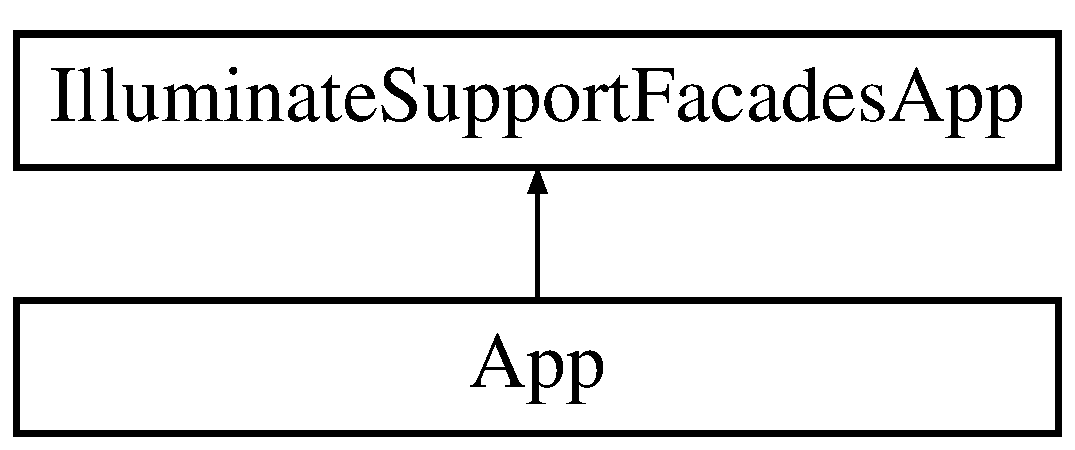
\includegraphics[height=2.000000cm]{class_illuminate_1_1_support_1_1_facades_1_1_app}
\end{center}
\end{figure}
\subsection*{Static Public Member Functions}
\begin{DoxyCompactItemize}
\item 
static \mbox{\hyperlink{class_illuminate_1_1_support_1_1_facades_1_1_app_af1d0616b31932a0e645e6264578a0243}{version}} ()
\item 
static \mbox{\hyperlink{class_illuminate_1_1_support_1_1_facades_1_1_app_a1397831bdc0a4d82c50c7435921d5053}{bootstrap\+With}} (\$bootstrappers)
\item 
static \mbox{\hyperlink{class_illuminate_1_1_support_1_1_facades_1_1_app_ad816001ccc8ba065c0eae100cb6de95f}{after\+Loading\+Environment}} (\$callback)
\item 
static \mbox{\hyperlink{class_illuminate_1_1_support_1_1_facades_1_1_app_a64563b5cc0a5d3a49f7eb6bc35c7e91a}{before\+Bootstrapping}} (\$bootstrapper, \$callback)
\item 
static \mbox{\hyperlink{class_illuminate_1_1_support_1_1_facades_1_1_app_a3aa4c683656337cf979b4552f69eca96}{after\+Bootstrapping}} (\$bootstrapper, \$callback)
\item 
static \mbox{\hyperlink{class_illuminate_1_1_support_1_1_facades_1_1_app_aa21c13916407cbc1db73a02d7c925ddf}{has\+Been\+Bootstrapped}} ()
\item 
static \mbox{\hyperlink{class_illuminate_1_1_support_1_1_facades_1_1_app_a13a02a2a5d8d2f2b54acfac91ad92fdd}{set\+Base\+Path}} (\$\mbox{\hyperlink{class_illuminate_1_1_support_1_1_facades_1_1_app_a144d9307a519b47a6f26f97cf761388c}{base\+Path}})
\item 
static \mbox{\hyperlink{class_illuminate_1_1_support_1_1_facades_1_1_app_a7200f5a02f461cd9329772f8fbffd35c}{path}} (\$path=\textquotesingle{}\textquotesingle{})
\item 
static \mbox{\hyperlink{class_illuminate_1_1_support_1_1_facades_1_1_app_a144d9307a519b47a6f26f97cf761388c}{base\+Path}} (\$\mbox{\hyperlink{class_illuminate_1_1_support_1_1_facades_1_1_app_a7200f5a02f461cd9329772f8fbffd35c}{path}}=\textquotesingle{}\textquotesingle{})
\item 
static \mbox{\hyperlink{class_illuminate_1_1_support_1_1_facades_1_1_app_a64bbb4c2fa9f4b9f064e1d30fe9633d2}{bootstrap\+Path}} (\$\mbox{\hyperlink{class_illuminate_1_1_support_1_1_facades_1_1_app_a7200f5a02f461cd9329772f8fbffd35c}{path}}=\textquotesingle{}\textquotesingle{})
\item 
static \mbox{\hyperlink{class_illuminate_1_1_support_1_1_facades_1_1_app_a845dcaea8494b510af1a452dd4bb99e6}{config\+Path}} (\$\mbox{\hyperlink{class_illuminate_1_1_support_1_1_facades_1_1_app_a7200f5a02f461cd9329772f8fbffd35c}{path}}=\textquotesingle{}\textquotesingle{})
\item 
static \mbox{\hyperlink{class_illuminate_1_1_support_1_1_facades_1_1_app_a6c5c735e7b038aec0a621faea3f5ce71}{database\+Path}} (\$\mbox{\hyperlink{class_illuminate_1_1_support_1_1_facades_1_1_app_a7200f5a02f461cd9329772f8fbffd35c}{path}}=\textquotesingle{}\textquotesingle{})
\item 
static \mbox{\hyperlink{class_illuminate_1_1_support_1_1_facades_1_1_app_aab597a19661bf87e58ffe52b40ee0d76}{use\+Database\+Path}} (\$\mbox{\hyperlink{class_illuminate_1_1_support_1_1_facades_1_1_app_a7200f5a02f461cd9329772f8fbffd35c}{path}})
\item 
static \mbox{\hyperlink{class_illuminate_1_1_support_1_1_facades_1_1_app_a1b94a2dee5cbf520b2b77096307b599a}{lang\+Path}} ()
\item 
static \mbox{\hyperlink{class_illuminate_1_1_support_1_1_facades_1_1_app_addeef28bcdf95f970e3a60d009d3d6c3}{public\+Path}} ()
\item 
static \mbox{\hyperlink{class_illuminate_1_1_support_1_1_facades_1_1_app_a9fe2d74a1df10fc44044ec6e7011d368}{storage\+Path}} ()
\item 
static \mbox{\hyperlink{class_illuminate_1_1_support_1_1_facades_1_1_app_ad31a72f91f6c5f3ed45971f3885aa1a8}{use\+Storage\+Path}} (\$\mbox{\hyperlink{class_illuminate_1_1_support_1_1_facades_1_1_app_a7200f5a02f461cd9329772f8fbffd35c}{path}})
\item 
static \mbox{\hyperlink{class_illuminate_1_1_support_1_1_facades_1_1_app_a55f49bd2192a4fa7f8b8934b618fbba8}{resource\+Path}} (\$\mbox{\hyperlink{class_illuminate_1_1_support_1_1_facades_1_1_app_a7200f5a02f461cd9329772f8fbffd35c}{path}}=\textquotesingle{}\textquotesingle{})
\item 
static \mbox{\hyperlink{class_illuminate_1_1_support_1_1_facades_1_1_app_a1807951e75c0a0c2430054252d62f1a4}{environment\+Path}} ()
\item 
static \mbox{\hyperlink{class_illuminate_1_1_support_1_1_facades_1_1_app_a6fab2dce6c54f875d1f6e41de50cdd38}{use\+Environment\+Path}} (\$\mbox{\hyperlink{class_illuminate_1_1_support_1_1_facades_1_1_app_a7200f5a02f461cd9329772f8fbffd35c}{path}})
\item 
static \mbox{\hyperlink{class_illuminate_1_1_support_1_1_facades_1_1_app_aa17fcc58971f3f99629a77d7422bec82}{load\+Environment\+From}} (\$file)
\item 
static \mbox{\hyperlink{class_illuminate_1_1_support_1_1_facades_1_1_app_a8e9f268a821fcc7aa3dcab483cb187f3}{environment\+File}} ()
\item 
static \mbox{\hyperlink{class_illuminate_1_1_support_1_1_facades_1_1_app_a9c16c89deae92c08b4e5d279c1a15ce8}{environment\+File\+Path}} ()
\item 
static \mbox{\hyperlink{class_illuminate_1_1_support_1_1_facades_1_1_app_a53c0fed127157d6e0bef9fbeb259f348}{environment}} ()
\item 
static \mbox{\hyperlink{class_illuminate_1_1_support_1_1_facades_1_1_app_af9c91947f215d034daffd62a0ce9567f}{is\+Local}} ()
\item 
static \mbox{\hyperlink{class_illuminate_1_1_support_1_1_facades_1_1_app_aeb4034f4059f16bcc57773dd9acfa0d8}{detect\+Environment}} (\$callback)
\item 
static \mbox{\hyperlink{class_illuminate_1_1_support_1_1_facades_1_1_app_a476511ac80c67bc70dc76a1042a6e865}{running\+In\+Console}} ()
\item 
static \mbox{\hyperlink{class_illuminate_1_1_support_1_1_facades_1_1_app_a446de3e653e69d73e1fb3472b461c62e}{running\+Unit\+Tests}} ()
\item 
static \mbox{\hyperlink{class_illuminate_1_1_support_1_1_facades_1_1_app_a710f47568d2719e075faa6a4c82efc9b}{register\+Configured\+Providers}} ()
\item 
static \mbox{\hyperlink{class_illuminate_1_1_support_1_1_facades_1_1_app_ac2e4bf09a742bb48073523175bd8af49}{register}} (\$provider, \$options=array(), \$force=false)
\item 
static \mbox{\hyperlink{class_illuminate_1_1_support_1_1_facades_1_1_app_ab2b9e7c49809a4eb07a43851556bb5c9}{get\+Provider}} (\$provider)
\item 
static \mbox{\hyperlink{class_illuminate_1_1_support_1_1_facades_1_1_app_ae97865b3b6812e19ccf40260ab4e7f42}{resolve\+Provider}} (\$provider)
\item 
static \mbox{\hyperlink{class_illuminate_1_1_support_1_1_facades_1_1_app_a159a31f00393c2604cf66d77b9e9f3a4}{load\+Deferred\+Providers}} ()
\item 
static \mbox{\hyperlink{class_illuminate_1_1_support_1_1_facades_1_1_app_a545876969ac4dc8564e16971a056994a}{load\+Deferred\+Provider}} (\$service)
\item 
static \mbox{\hyperlink{class_illuminate_1_1_support_1_1_facades_1_1_app_a889b60d8f2bfb4727bf4b79e640041ec}{register\+Deferred\+Provider}} (\$provider, \$service=null)
\item 
static \mbox{\hyperlink{class_illuminate_1_1_support_1_1_facades_1_1_app_a9087a869e39848f508cbdfa818b4a454}{make}} (\$abstract, \$parameters=array())
\item 
static \mbox{\hyperlink{class_illuminate_1_1_support_1_1_facades_1_1_app_aa6d5af98bdd9a231d94c84e2a043ee5a}{bound}} (\$abstract)
\item 
static \mbox{\hyperlink{class_illuminate_1_1_support_1_1_facades_1_1_app_a91c8977631218fb1ac7567a28f5e0fd5}{is\+Booted}} ()
\item 
static \mbox{\hyperlink{class_illuminate_1_1_support_1_1_facades_1_1_app_a16111fedc54691f0dedb21575c3bad06}{boot}} ()
\item 
static \mbox{\hyperlink{class_illuminate_1_1_support_1_1_facades_1_1_app_a6e0a1ea8829091159951d60b5b5b11f3}{booting}} (\$callback)
\item 
static \mbox{\hyperlink{class_illuminate_1_1_support_1_1_facades_1_1_app_a066383a4a716aa8a23376781d90a0c87}{booted}} (\$callback)
\item 
static \mbox{\hyperlink{class_illuminate_1_1_support_1_1_facades_1_1_app_a291c55e10567a9c70b8df904fbfc0dcf}{handle}} (\$request, \$type=1, \$catch=true)
\item 
static \mbox{\hyperlink{class_illuminate_1_1_support_1_1_facades_1_1_app_a10f125eb3c7536818ed2cfe0458e179b}{should\+Skip\+Middleware}} ()
\item 
static \mbox{\hyperlink{class_illuminate_1_1_support_1_1_facades_1_1_app_a3bee1241aff9a729fe35c6e33046874d}{get\+Cached\+Services\+Path}} ()
\item 
static \mbox{\hyperlink{class_illuminate_1_1_support_1_1_facades_1_1_app_ab0155c3a224efa33a4683fdaf7d5d6ea}{get\+Cached\+Packages\+Path}} ()
\item 
static \mbox{\hyperlink{class_illuminate_1_1_support_1_1_facades_1_1_app_adb1cfc609d273f015bb69a56a958252f}{configuration\+Is\+Cached}} ()
\item 
static \mbox{\hyperlink{class_illuminate_1_1_support_1_1_facades_1_1_app_a231ce9e7ff90f62295b0ddc8b6cdd2a1}{get\+Cached\+Config\+Path}} ()
\item 
static \mbox{\hyperlink{class_illuminate_1_1_support_1_1_facades_1_1_app_a9ba11e68d2803f0c1d9f6fa33bf2f4e0}{routes\+Are\+Cached}} ()
\item 
static \mbox{\hyperlink{class_illuminate_1_1_support_1_1_facades_1_1_app_ae516b37acb35a241b58c5ae908fe446e}{get\+Cached\+Routes\+Path}} ()
\item 
static \mbox{\hyperlink{class_illuminate_1_1_support_1_1_facades_1_1_app_ab5121c618705672d1cb2e049705da6d4}{is\+Down\+For\+Maintenance}} ()
\item 
static \mbox{\hyperlink{class_illuminate_1_1_support_1_1_facades_1_1_app_a75aaa57ba29807d1e66c4819b33e4efb}{abort}} (\$code, \$message=\textquotesingle{}\textquotesingle{}, \$headers=array())
\item 
static \mbox{\hyperlink{class_illuminate_1_1_support_1_1_facades_1_1_app_aaa82ebd6ba2bf6af580669b2a15b1196}{terminating}} (\$callback)
\item 
static \mbox{\hyperlink{class_illuminate_1_1_support_1_1_facades_1_1_app_a982768aceae29a845b008c99edd5e03b}{terminate}} ()
\item 
static \mbox{\hyperlink{class_illuminate_1_1_support_1_1_facades_1_1_app_aad297b9ed28f650dae1721e05df5d997}{get\+Loaded\+Providers}} ()
\item 
static \mbox{\hyperlink{class_illuminate_1_1_support_1_1_facades_1_1_app_a8898e3fcdc4d57c73ca8dd9c3eeb27b6}{get\+Deferred\+Services}} ()
\item 
static \mbox{\hyperlink{class_illuminate_1_1_support_1_1_facades_1_1_app_ac74a1a0bfe5c595e1714f344bbc3c410}{set\+Deferred\+Services}} (\$services)
\item 
static \mbox{\hyperlink{class_illuminate_1_1_support_1_1_facades_1_1_app_af63352b358d10632ec6537aacf2b0933}{add\+Deferred\+Services}} (\$services)
\item 
static \mbox{\hyperlink{class_illuminate_1_1_support_1_1_facades_1_1_app_a9e6bba2ff3db437fd8af4f59225c1601}{is\+Deferred\+Service}} (\$service)
\item 
static \mbox{\hyperlink{class_illuminate_1_1_support_1_1_facades_1_1_app_acb93eb8d4d24729b8264c00e5b94dfb1}{provide\+Facades}} (\$namespace)
\item 
static \mbox{\hyperlink{class_illuminate_1_1_support_1_1_facades_1_1_app_aeba7c2058e2b423b7f5ed5a49e69c669}{configure\+Monolog\+Using}} (\$callback)
\item 
static \mbox{\hyperlink{class_illuminate_1_1_support_1_1_facades_1_1_app_aab82809a204086b615e445bea282d58b}{has\+Monolog\+Configurator}} ()
\item 
static \mbox{\hyperlink{class_illuminate_1_1_support_1_1_facades_1_1_app_a10d6104d2082582c9b60e90a344bb02e}{get\+Monolog\+Configurator}} ()
\item 
static \mbox{\hyperlink{class_illuminate_1_1_support_1_1_facades_1_1_app_a7c40fc2b0fa689f7731b77dc910ee1b3}{get\+Locale}} ()
\item 
static \mbox{\hyperlink{class_illuminate_1_1_support_1_1_facades_1_1_app_a8086d8d1be8bc33af2730f4a23f8dd7d}{set\+Locale}} (\$locale)
\item 
static \mbox{\hyperlink{class_illuminate_1_1_support_1_1_facades_1_1_app_aaf446792c0b06fd9d8ae04eaf49bd0f3}{is\+Locale}} (\$locale)
\item 
static \mbox{\hyperlink{class_illuminate_1_1_support_1_1_facades_1_1_app_aa40d73f464d8ea9b6773de92627724ba}{register\+Core\+Container\+Aliases}} ()
\item 
static \mbox{\hyperlink{class_illuminate_1_1_support_1_1_facades_1_1_app_a168870a69340a27e4d660cbcf7189558}{flush}} ()
\item 
static \mbox{\hyperlink{class_illuminate_1_1_support_1_1_facades_1_1_app_ab9efc7221fd51924278d9a959348a556}{get\+Namespace}} ()
\item 
static \mbox{\hyperlink{class_illuminate_1_1_support_1_1_facades_1_1_app_a9255963e97fbfb9128c9dd66e60c0d36}{when}} (\$concrete)
\item 
static \mbox{\hyperlink{class_illuminate_1_1_support_1_1_facades_1_1_app_a86f6f04a4b68b1a96c67b8b5cd5e1c39}{has}} (\$id)
\item 
static \mbox{\hyperlink{class_illuminate_1_1_support_1_1_facades_1_1_app_ae7d043eb1da4cdba908ddcacdeb7ad67}{resolved}} (\$abstract)
\item 
static \mbox{\hyperlink{class_illuminate_1_1_support_1_1_facades_1_1_app_a345cc220f504fb29e2345e66f4817a4a}{is\+Shared}} (\$abstract)
\item 
static \mbox{\hyperlink{class_illuminate_1_1_support_1_1_facades_1_1_app_afaf25e56d5c74d2bc97da60866fdc73a}{is\+Alias}} (\$name)
\item 
static \mbox{\hyperlink{class_illuminate_1_1_support_1_1_facades_1_1_app_a3957346546b9adf11c0914ff37367685}{bind}} (\$abstract, \$concrete=null, \$shared=false)
\item 
static \mbox{\hyperlink{class_illuminate_1_1_support_1_1_facades_1_1_app_acd3b7dbd6fff0001ea04ce38b06215c1}{has\+Method\+Binding}} (\$method)
\item 
static \mbox{\hyperlink{class_illuminate_1_1_support_1_1_facades_1_1_app_a5448282fe52aa12e5b1b2d6c6b3172f4}{bind\+Method}} (\$method, \$callback)
\item 
static \mbox{\hyperlink{class_illuminate_1_1_support_1_1_facades_1_1_app_abbf90ce34d22de29e1f0d12e6d11c14f}{call\+Method\+Binding}} (\$method, \$\mbox{\hyperlink{class_illuminate_1_1_support_1_1_facades_1_1_app_aec0719063c5b42f03d9755ca1cddb4a5}{instance}})
\item 
static \mbox{\hyperlink{class_illuminate_1_1_support_1_1_facades_1_1_app_ae0afa82b6a8d53c806ae365e7626bd07}{add\+Contextual\+Binding}} (\$concrete, \$abstract, \$implementation)
\item 
static \mbox{\hyperlink{class_illuminate_1_1_support_1_1_facades_1_1_app_a8db40bfe0c2b3a1c4ede6815ce71abc5}{bind\+If}} (\$abstract, \$concrete=null, \$shared=false)
\item 
static \mbox{\hyperlink{class_illuminate_1_1_support_1_1_facades_1_1_app_a893f2164a679be5778ef2f61e66ce483}{singleton}} (\$abstract, \$concrete=null)
\item 
static \mbox{\hyperlink{class_illuminate_1_1_support_1_1_facades_1_1_app_afc2cde60d0741918d47b74fb55240f2a}{extend}} (\$abstract, \$closure)
\item 
static \mbox{\hyperlink{class_illuminate_1_1_support_1_1_facades_1_1_app_aec0719063c5b42f03d9755ca1cddb4a5}{instance}} (\$abstract, \$instance)
\item 
static \mbox{\hyperlink{class_illuminate_1_1_support_1_1_facades_1_1_app_a7e64d002f0ed1005ecda67ca49ef254d}{tag}} (\$abstracts, \$tags)
\item 
static \mbox{\hyperlink{class_illuminate_1_1_support_1_1_facades_1_1_app_a82a57ed32c484ce85898ea2f88ac382f}{tagged}} (\$\mbox{\hyperlink{class_illuminate_1_1_support_1_1_facades_1_1_app_a7e64d002f0ed1005ecda67ca49ef254d}{tag}})
\item 
static \mbox{\hyperlink{class_illuminate_1_1_support_1_1_facades_1_1_app_a1b1fecb6264e98b03b1216e0e8976649}{alias}} (\$abstract, \$alias)
\item 
static \mbox{\hyperlink{class_illuminate_1_1_support_1_1_facades_1_1_app_a339861dbb69a8272f82ea394089c98c1}{rebinding}} (\$abstract, \$callback)
\item 
static \mbox{\hyperlink{class_illuminate_1_1_support_1_1_facades_1_1_app_a778ca58f7e376f07cbc7718aa03bd681}{refresh}} (\$abstract, \$target, \$method)
\item 
static \mbox{\hyperlink{class_illuminate_1_1_support_1_1_facades_1_1_app_a02a59d234efa1d1ca364e08584a14d34}{wrap}} (\$callback, \$parameters=array())
\item 
static \mbox{\hyperlink{class_illuminate_1_1_support_1_1_facades_1_1_app_abdb4bfe6bdc04b28d4adb6572d976fd9}{call}} (\$callback, \$parameters=array(), \$default\+Method=null)
\item 
static \mbox{\hyperlink{class_illuminate_1_1_support_1_1_facades_1_1_app_a367f484711c4a6b30fa94b18f6c7a87a}{factory}} (\$abstract)
\item 
static \mbox{\hyperlink{class_illuminate_1_1_support_1_1_facades_1_1_app_a21185e146da59bcf6b7e5dfb658af27e}{make\+With}} (\$abstract, \$parameters=array())
\item 
static \mbox{\hyperlink{class_illuminate_1_1_support_1_1_facades_1_1_app_a042054c3892563f7f0b31cb9e1c9bb76}{get}} (\$id)
\item 
static \mbox{\hyperlink{class_illuminate_1_1_support_1_1_facades_1_1_app_afc58bf4ad412d93583b845767132ac6a}{build}} (\$concrete)
\item 
static \mbox{\hyperlink{class_illuminate_1_1_support_1_1_facades_1_1_app_a9f7b165d7ce251ca9f5a8151efc7cf81}{resolving}} (\$abstract, \$callback=null)
\item 
static \mbox{\hyperlink{class_illuminate_1_1_support_1_1_facades_1_1_app_a51d11cc845124fdb0f345deffac0246c}{after\+Resolving}} (\$abstract, \$callback=null)
\item 
static \mbox{\hyperlink{class_illuminate_1_1_support_1_1_facades_1_1_app_aa54235f81ed08702ae31cfc2cd4f8f2a}{get\+Bindings}} ()
\item 
static \mbox{\hyperlink{class_illuminate_1_1_support_1_1_facades_1_1_app_a332b40e237f5eed64e3b5c26a9198922}{get\+Alias}} (\$abstract)
\item 
static \mbox{\hyperlink{class_illuminate_1_1_support_1_1_facades_1_1_app_a45a3221fbedd5979dd94c53588d57788}{forget\+Extenders}} (\$abstract)
\item 
static \mbox{\hyperlink{class_illuminate_1_1_support_1_1_facades_1_1_app_a247958d883cadf721387a38630e09206}{forget\+Instance}} (\$abstract)
\item 
static \mbox{\hyperlink{class_illuminate_1_1_support_1_1_facades_1_1_app_ae2ba5f8713c76ac249c9c1284e656dca}{forget\+Instances}} ()
\item 
static \mbox{\hyperlink{class_illuminate_1_1_support_1_1_facades_1_1_app_a804a809eeccf0c334dd07c079029bee3}{get\+Instance}} ()
\item 
static \mbox{\hyperlink{class_illuminate_1_1_support_1_1_facades_1_1_app_a175fcd9533e4df56e2b8bb161e7d3c4a}{set\+Instance}} (\$container=null)
\item 
static \mbox{\hyperlink{class_illuminate_1_1_support_1_1_facades_1_1_app_a998154ab84d493b5d6a4b4df8cc219e1}{offset\+Exists}} (\$key)
\item 
static \mbox{\hyperlink{class_illuminate_1_1_support_1_1_facades_1_1_app_a97d7d94e05f76b4f6d210129a0755283}{offset\+Get}} (\$key)
\item 
static \mbox{\hyperlink{class_illuminate_1_1_support_1_1_facades_1_1_app_a9d295382cd64e5055d031c71a0edecaf}{offset\+Set}} (\$key, \$value)
\item 
static \mbox{\hyperlink{class_illuminate_1_1_support_1_1_facades_1_1_app_a9fed51d2c46e6cc3d943f9835c42628f}{offset\+Unset}} (\$key)
\end{DoxyCompactItemize}


\subsection{Member Function Documentation}
\mbox{\Hypertarget{class_illuminate_1_1_support_1_1_facades_1_1_app_a75aaa57ba29807d1e66c4819b33e4efb}\label{class_illuminate_1_1_support_1_1_facades_1_1_app_a75aaa57ba29807d1e66c4819b33e4efb}} 
\index{Illuminate\+::\+Support\+::\+Facades\+::\+App@{Illuminate\+::\+Support\+::\+Facades\+::\+App}!abort@{abort}}
\index{abort@{abort}!Illuminate\+::\+Support\+::\+Facades\+::\+App@{Illuminate\+::\+Support\+::\+Facades\+::\+App}}
\subsubsection{\texorpdfstring{abort()}{abort()}}
{\footnotesize\ttfamily static Illuminate\textbackslash{}\+Support\textbackslash{}\+Facades\textbackslash{}\+App\+::abort (\begin{DoxyParamCaption}\item[{}]{\$code,  }\item[{}]{\$message = {\ttfamily \textquotesingle{}\textquotesingle{}},  }\item[{}]{\$headers = {\ttfamily array()} }\end{DoxyParamCaption})\hspace{0.3cm}{\ttfamily [static]}}

Throw an Http\+Exception with the given data.


\begin{DoxyParams}[1]{Parameters}
int & {\em \$code} & \\
\hline
string & {\em \$message} & \\
\hline
array & {\em \$headers} & \\
\hline
\end{DoxyParams}
\begin{DoxyReturn}{Returns}
void 
\end{DoxyReturn}

\begin{DoxyExceptions}{Exceptions}
{\em } & \\
\hline
\end{DoxyExceptions}
\mbox{\Hypertarget{class_illuminate_1_1_support_1_1_facades_1_1_app_ae0afa82b6a8d53c806ae365e7626bd07}\label{class_illuminate_1_1_support_1_1_facades_1_1_app_ae0afa82b6a8d53c806ae365e7626bd07}} 
\index{Illuminate\+::\+Support\+::\+Facades\+::\+App@{Illuminate\+::\+Support\+::\+Facades\+::\+App}!add\+Contextual\+Binding@{add\+Contextual\+Binding}}
\index{add\+Contextual\+Binding@{add\+Contextual\+Binding}!Illuminate\+::\+Support\+::\+Facades\+::\+App@{Illuminate\+::\+Support\+::\+Facades\+::\+App}}
\subsubsection{\texorpdfstring{add\+Contextual\+Binding()}{addContextualBinding()}}
{\footnotesize\ttfamily static Illuminate\textbackslash{}\+Support\textbackslash{}\+Facades\textbackslash{}\+App\+::add\+Contextual\+Binding (\begin{DoxyParamCaption}\item[{}]{\$concrete,  }\item[{}]{\$abstract,  }\item[{}]{\$implementation }\end{DoxyParamCaption})\hspace{0.3cm}{\ttfamily [static]}}

Add a contextual binding to the container.


\begin{DoxyParams}[1]{Parameters}
string & {\em \$concrete} & \\
\hline
string & {\em \$abstract} & \\
\hline
\textbackslash{}\+Closure | string & {\em \$implementation} & \\
\hline
\end{DoxyParams}
\begin{DoxyReturn}{Returns}
void 
\end{DoxyReturn}
\mbox{\Hypertarget{class_illuminate_1_1_support_1_1_facades_1_1_app_af63352b358d10632ec6537aacf2b0933}\label{class_illuminate_1_1_support_1_1_facades_1_1_app_af63352b358d10632ec6537aacf2b0933}} 
\index{Illuminate\+::\+Support\+::\+Facades\+::\+App@{Illuminate\+::\+Support\+::\+Facades\+::\+App}!add\+Deferred\+Services@{add\+Deferred\+Services}}
\index{add\+Deferred\+Services@{add\+Deferred\+Services}!Illuminate\+::\+Support\+::\+Facades\+::\+App@{Illuminate\+::\+Support\+::\+Facades\+::\+App}}
\subsubsection{\texorpdfstring{add\+Deferred\+Services()}{addDeferredServices()}}
{\footnotesize\ttfamily static Illuminate\textbackslash{}\+Support\textbackslash{}\+Facades\textbackslash{}\+App\+::add\+Deferred\+Services (\begin{DoxyParamCaption}\item[{}]{\$services }\end{DoxyParamCaption})\hspace{0.3cm}{\ttfamily [static]}}

Add an array of services to the application\textquotesingle{}s deferred services.


\begin{DoxyParams}[1]{Parameters}
array & {\em \$services} & \\
\hline
\end{DoxyParams}
\begin{DoxyReturn}{Returns}
void 
\end{DoxyReturn}
\mbox{\Hypertarget{class_illuminate_1_1_support_1_1_facades_1_1_app_a3aa4c683656337cf979b4552f69eca96}\label{class_illuminate_1_1_support_1_1_facades_1_1_app_a3aa4c683656337cf979b4552f69eca96}} 
\index{Illuminate\+::\+Support\+::\+Facades\+::\+App@{Illuminate\+::\+Support\+::\+Facades\+::\+App}!after\+Bootstrapping@{after\+Bootstrapping}}
\index{after\+Bootstrapping@{after\+Bootstrapping}!Illuminate\+::\+Support\+::\+Facades\+::\+App@{Illuminate\+::\+Support\+::\+Facades\+::\+App}}
\subsubsection{\texorpdfstring{after\+Bootstrapping()}{afterBootstrapping()}}
{\footnotesize\ttfamily static Illuminate\textbackslash{}\+Support\textbackslash{}\+Facades\textbackslash{}\+App\+::after\+Bootstrapping (\begin{DoxyParamCaption}\item[{}]{\$bootstrapper,  }\item[{}]{\$callback }\end{DoxyParamCaption})\hspace{0.3cm}{\ttfamily [static]}}

Register a callback to run after a bootstrapper.


\begin{DoxyParams}[1]{Parameters}
string & {\em \$bootstrapper} & \\
\hline
\textbackslash{}\+Closure & {\em \$callback} & \\
\hline
\end{DoxyParams}
\begin{DoxyReturn}{Returns}
void 
\end{DoxyReturn}
\mbox{\Hypertarget{class_illuminate_1_1_support_1_1_facades_1_1_app_ad816001ccc8ba065c0eae100cb6de95f}\label{class_illuminate_1_1_support_1_1_facades_1_1_app_ad816001ccc8ba065c0eae100cb6de95f}} 
\index{Illuminate\+::\+Support\+::\+Facades\+::\+App@{Illuminate\+::\+Support\+::\+Facades\+::\+App}!after\+Loading\+Environment@{after\+Loading\+Environment}}
\index{after\+Loading\+Environment@{after\+Loading\+Environment}!Illuminate\+::\+Support\+::\+Facades\+::\+App@{Illuminate\+::\+Support\+::\+Facades\+::\+App}}
\subsubsection{\texorpdfstring{after\+Loading\+Environment()}{afterLoadingEnvironment()}}
{\footnotesize\ttfamily static Illuminate\textbackslash{}\+Support\textbackslash{}\+Facades\textbackslash{}\+App\+::after\+Loading\+Environment (\begin{DoxyParamCaption}\item[{}]{\$callback }\end{DoxyParamCaption})\hspace{0.3cm}{\ttfamily [static]}}

Register a callback to run after loading the environment.


\begin{DoxyParams}[1]{Parameters}
\textbackslash{}\+Closure & {\em \$callback} & \\
\hline
\end{DoxyParams}
\begin{DoxyReturn}{Returns}
void 
\end{DoxyReturn}
\mbox{\Hypertarget{class_illuminate_1_1_support_1_1_facades_1_1_app_a51d11cc845124fdb0f345deffac0246c}\label{class_illuminate_1_1_support_1_1_facades_1_1_app_a51d11cc845124fdb0f345deffac0246c}} 
\index{Illuminate\+::\+Support\+::\+Facades\+::\+App@{Illuminate\+::\+Support\+::\+Facades\+::\+App}!after\+Resolving@{after\+Resolving}}
\index{after\+Resolving@{after\+Resolving}!Illuminate\+::\+Support\+::\+Facades\+::\+App@{Illuminate\+::\+Support\+::\+Facades\+::\+App}}
\subsubsection{\texorpdfstring{after\+Resolving()}{afterResolving()}}
{\footnotesize\ttfamily static Illuminate\textbackslash{}\+Support\textbackslash{}\+Facades\textbackslash{}\+App\+::after\+Resolving (\begin{DoxyParamCaption}\item[{}]{\$abstract,  }\item[{}]{\$callback = {\ttfamily null} }\end{DoxyParamCaption})\hspace{0.3cm}{\ttfamily [static]}}

Register a new after resolving callback for all types.


\begin{DoxyParams}[1]{Parameters}
string & {\em \$abstract} & \\
\hline
\textbackslash{}\+Closure | null & {\em \$callback} & \\
\hline
\end{DoxyParams}
\begin{DoxyReturn}{Returns}
void 
\end{DoxyReturn}
\mbox{\Hypertarget{class_illuminate_1_1_support_1_1_facades_1_1_app_a1b1fecb6264e98b03b1216e0e8976649}\label{class_illuminate_1_1_support_1_1_facades_1_1_app_a1b1fecb6264e98b03b1216e0e8976649}} 
\index{Illuminate\+::\+Support\+::\+Facades\+::\+App@{Illuminate\+::\+Support\+::\+Facades\+::\+App}!alias@{alias}}
\index{alias@{alias}!Illuminate\+::\+Support\+::\+Facades\+::\+App@{Illuminate\+::\+Support\+::\+Facades\+::\+App}}
\subsubsection{\texorpdfstring{alias()}{alias()}}
{\footnotesize\ttfamily static Illuminate\textbackslash{}\+Support\textbackslash{}\+Facades\textbackslash{}\+App\+::alias (\begin{DoxyParamCaption}\item[{}]{\$abstract,  }\item[{}]{\$alias }\end{DoxyParamCaption})\hspace{0.3cm}{\ttfamily [static]}}

Alias a type to a different name.


\begin{DoxyParams}[1]{Parameters}
string & {\em \$abstract} & \\
\hline
string & {\em \$alias} & \\
\hline
\end{DoxyParams}
\begin{DoxyReturn}{Returns}
void 
\end{DoxyReturn}
\mbox{\Hypertarget{class_illuminate_1_1_support_1_1_facades_1_1_app_a144d9307a519b47a6f26f97cf761388c}\label{class_illuminate_1_1_support_1_1_facades_1_1_app_a144d9307a519b47a6f26f97cf761388c}} 
\index{Illuminate\+::\+Support\+::\+Facades\+::\+App@{Illuminate\+::\+Support\+::\+Facades\+::\+App}!base\+Path@{base\+Path}}
\index{base\+Path@{base\+Path}!Illuminate\+::\+Support\+::\+Facades\+::\+App@{Illuminate\+::\+Support\+::\+Facades\+::\+App}}
\subsubsection{\texorpdfstring{base\+Path()}{basePath()}}
{\footnotesize\ttfamily static Illuminate\textbackslash{}\+Support\textbackslash{}\+Facades\textbackslash{}\+App\+::base\+Path (\begin{DoxyParamCaption}\item[{}]{\$path = {\ttfamily \textquotesingle{}\textquotesingle{}} }\end{DoxyParamCaption})\hspace{0.3cm}{\ttfamily [static]}}

Get the base path of the \mbox{\hyperlink{namespace_laravel}{Laravel}} installation.


\begin{DoxyParams}[1]{Parameters}
string & {\em \$path} & Optionally, a path to append to the base path \\
\hline
\end{DoxyParams}
\begin{DoxyReturn}{Returns}
string 
\end{DoxyReturn}
\mbox{\Hypertarget{class_illuminate_1_1_support_1_1_facades_1_1_app_a64563b5cc0a5d3a49f7eb6bc35c7e91a}\label{class_illuminate_1_1_support_1_1_facades_1_1_app_a64563b5cc0a5d3a49f7eb6bc35c7e91a}} 
\index{Illuminate\+::\+Support\+::\+Facades\+::\+App@{Illuminate\+::\+Support\+::\+Facades\+::\+App}!before\+Bootstrapping@{before\+Bootstrapping}}
\index{before\+Bootstrapping@{before\+Bootstrapping}!Illuminate\+::\+Support\+::\+Facades\+::\+App@{Illuminate\+::\+Support\+::\+Facades\+::\+App}}
\subsubsection{\texorpdfstring{before\+Bootstrapping()}{beforeBootstrapping()}}
{\footnotesize\ttfamily static Illuminate\textbackslash{}\+Support\textbackslash{}\+Facades\textbackslash{}\+App\+::before\+Bootstrapping (\begin{DoxyParamCaption}\item[{}]{\$bootstrapper,  }\item[{}]{\$callback }\end{DoxyParamCaption})\hspace{0.3cm}{\ttfamily [static]}}

Register a callback to run before a bootstrapper.


\begin{DoxyParams}[1]{Parameters}
string & {\em \$bootstrapper} & \\
\hline
\textbackslash{}\+Closure & {\em \$callback} & \\
\hline
\end{DoxyParams}
\begin{DoxyReturn}{Returns}
void 
\end{DoxyReturn}
\mbox{\Hypertarget{class_illuminate_1_1_support_1_1_facades_1_1_app_a3957346546b9adf11c0914ff37367685}\label{class_illuminate_1_1_support_1_1_facades_1_1_app_a3957346546b9adf11c0914ff37367685}} 
\index{Illuminate\+::\+Support\+::\+Facades\+::\+App@{Illuminate\+::\+Support\+::\+Facades\+::\+App}!bind@{bind}}
\index{bind@{bind}!Illuminate\+::\+Support\+::\+Facades\+::\+App@{Illuminate\+::\+Support\+::\+Facades\+::\+App}}
\subsubsection{\texorpdfstring{bind()}{bind()}}
{\footnotesize\ttfamily static Illuminate\textbackslash{}\+Support\textbackslash{}\+Facades\textbackslash{}\+App\+::bind (\begin{DoxyParamCaption}\item[{}]{\$abstract,  }\item[{}]{\$concrete = {\ttfamily null},  }\item[{}]{\$shared = {\ttfamily false} }\end{DoxyParamCaption})\hspace{0.3cm}{\ttfamily [static]}}

Register a binding with the container.


\begin{DoxyParams}[1]{Parameters}
string | array & {\em \$abstract} & \\
\hline
\textbackslash{}\+Closure | string | null & {\em \$concrete} & \\
\hline
bool & {\em \$shared} & \\
\hline
\end{DoxyParams}
\begin{DoxyReturn}{Returns}
void 
\end{DoxyReturn}
\mbox{\Hypertarget{class_illuminate_1_1_support_1_1_facades_1_1_app_a8db40bfe0c2b3a1c4ede6815ce71abc5}\label{class_illuminate_1_1_support_1_1_facades_1_1_app_a8db40bfe0c2b3a1c4ede6815ce71abc5}} 
\index{Illuminate\+::\+Support\+::\+Facades\+::\+App@{Illuminate\+::\+Support\+::\+Facades\+::\+App}!bind\+If@{bind\+If}}
\index{bind\+If@{bind\+If}!Illuminate\+::\+Support\+::\+Facades\+::\+App@{Illuminate\+::\+Support\+::\+Facades\+::\+App}}
\subsubsection{\texorpdfstring{bind\+If()}{bindIf()}}
{\footnotesize\ttfamily static Illuminate\textbackslash{}\+Support\textbackslash{}\+Facades\textbackslash{}\+App\+::bind\+If (\begin{DoxyParamCaption}\item[{}]{\$abstract,  }\item[{}]{\$concrete = {\ttfamily null},  }\item[{}]{\$shared = {\ttfamily false} }\end{DoxyParamCaption})\hspace{0.3cm}{\ttfamily [static]}}

Register a binding if it hasn\textquotesingle{}t already been registered.


\begin{DoxyParams}[1]{Parameters}
string & {\em \$abstract} & \\
\hline
\textbackslash{}\+Closure | string | null & {\em \$concrete} & \\
\hline
bool & {\em \$shared} & \\
\hline
\end{DoxyParams}
\begin{DoxyReturn}{Returns}
void 
\end{DoxyReturn}
\mbox{\Hypertarget{class_illuminate_1_1_support_1_1_facades_1_1_app_a5448282fe52aa12e5b1b2d6c6b3172f4}\label{class_illuminate_1_1_support_1_1_facades_1_1_app_a5448282fe52aa12e5b1b2d6c6b3172f4}} 
\index{Illuminate\+::\+Support\+::\+Facades\+::\+App@{Illuminate\+::\+Support\+::\+Facades\+::\+App}!bind\+Method@{bind\+Method}}
\index{bind\+Method@{bind\+Method}!Illuminate\+::\+Support\+::\+Facades\+::\+App@{Illuminate\+::\+Support\+::\+Facades\+::\+App}}
\subsubsection{\texorpdfstring{bind\+Method()}{bindMethod()}}
{\footnotesize\ttfamily static Illuminate\textbackslash{}\+Support\textbackslash{}\+Facades\textbackslash{}\+App\+::bind\+Method (\begin{DoxyParamCaption}\item[{}]{\$method,  }\item[{}]{\$callback }\end{DoxyParamCaption})\hspace{0.3cm}{\ttfamily [static]}}

Bind a callback to resolve with Container\+::call.


\begin{DoxyParams}[1]{Parameters}
string & {\em \$method} & \\
\hline
\textbackslash{}\+Closure & {\em \$callback} & \\
\hline
\end{DoxyParams}
\begin{DoxyReturn}{Returns}
void 
\end{DoxyReturn}
\mbox{\Hypertarget{class_illuminate_1_1_support_1_1_facades_1_1_app_a16111fedc54691f0dedb21575c3bad06}\label{class_illuminate_1_1_support_1_1_facades_1_1_app_a16111fedc54691f0dedb21575c3bad06}} 
\index{Illuminate\+::\+Support\+::\+Facades\+::\+App@{Illuminate\+::\+Support\+::\+Facades\+::\+App}!boot@{boot}}
\index{boot@{boot}!Illuminate\+::\+Support\+::\+Facades\+::\+App@{Illuminate\+::\+Support\+::\+Facades\+::\+App}}
\subsubsection{\texorpdfstring{boot()}{boot()}}
{\footnotesize\ttfamily static Illuminate\textbackslash{}\+Support\textbackslash{}\+Facades\textbackslash{}\+App\+::boot (\begin{DoxyParamCaption}{ }\end{DoxyParamCaption})\hspace{0.3cm}{\ttfamily [static]}}

Boot the application\textquotesingle{}s service providers.

\begin{DoxyReturn}{Returns}
void 
\end{DoxyReturn}
\mbox{\Hypertarget{class_illuminate_1_1_support_1_1_facades_1_1_app_a066383a4a716aa8a23376781d90a0c87}\label{class_illuminate_1_1_support_1_1_facades_1_1_app_a066383a4a716aa8a23376781d90a0c87}} 
\index{Illuminate\+::\+Support\+::\+Facades\+::\+App@{Illuminate\+::\+Support\+::\+Facades\+::\+App}!booted@{booted}}
\index{booted@{booted}!Illuminate\+::\+Support\+::\+Facades\+::\+App@{Illuminate\+::\+Support\+::\+Facades\+::\+App}}
\subsubsection{\texorpdfstring{booted()}{booted()}}
{\footnotesize\ttfamily static Illuminate\textbackslash{}\+Support\textbackslash{}\+Facades\textbackslash{}\+App\+::booted (\begin{DoxyParamCaption}\item[{}]{\$callback }\end{DoxyParamCaption})\hspace{0.3cm}{\ttfamily [static]}}

Register a new \char`\"{}booted\char`\"{} listener.


\begin{DoxyParams}[1]{Parameters}
mixed & {\em \$callback} & \\
\hline
\end{DoxyParams}
\begin{DoxyReturn}{Returns}
void 
\end{DoxyReturn}
\mbox{\Hypertarget{class_illuminate_1_1_support_1_1_facades_1_1_app_a6e0a1ea8829091159951d60b5b5b11f3}\label{class_illuminate_1_1_support_1_1_facades_1_1_app_a6e0a1ea8829091159951d60b5b5b11f3}} 
\index{Illuminate\+::\+Support\+::\+Facades\+::\+App@{Illuminate\+::\+Support\+::\+Facades\+::\+App}!booting@{booting}}
\index{booting@{booting}!Illuminate\+::\+Support\+::\+Facades\+::\+App@{Illuminate\+::\+Support\+::\+Facades\+::\+App}}
\subsubsection{\texorpdfstring{booting()}{booting()}}
{\footnotesize\ttfamily static Illuminate\textbackslash{}\+Support\textbackslash{}\+Facades\textbackslash{}\+App\+::booting (\begin{DoxyParamCaption}\item[{}]{\$callback }\end{DoxyParamCaption})\hspace{0.3cm}{\ttfamily [static]}}

Register a new boot listener.


\begin{DoxyParams}[1]{Parameters}
mixed & {\em \$callback} & \\
\hline
\end{DoxyParams}
\begin{DoxyReturn}{Returns}
void 
\end{DoxyReturn}
\mbox{\Hypertarget{class_illuminate_1_1_support_1_1_facades_1_1_app_a64bbb4c2fa9f4b9f064e1d30fe9633d2}\label{class_illuminate_1_1_support_1_1_facades_1_1_app_a64bbb4c2fa9f4b9f064e1d30fe9633d2}} 
\index{Illuminate\+::\+Support\+::\+Facades\+::\+App@{Illuminate\+::\+Support\+::\+Facades\+::\+App}!bootstrap\+Path@{bootstrap\+Path}}
\index{bootstrap\+Path@{bootstrap\+Path}!Illuminate\+::\+Support\+::\+Facades\+::\+App@{Illuminate\+::\+Support\+::\+Facades\+::\+App}}
\subsubsection{\texorpdfstring{bootstrap\+Path()}{bootstrapPath()}}
{\footnotesize\ttfamily static Illuminate\textbackslash{}\+Support\textbackslash{}\+Facades\textbackslash{}\+App\+::bootstrap\+Path (\begin{DoxyParamCaption}\item[{}]{\$path = {\ttfamily \textquotesingle{}\textquotesingle{}} }\end{DoxyParamCaption})\hspace{0.3cm}{\ttfamily [static]}}

Get the path to the bootstrap directory.


\begin{DoxyParams}[1]{Parameters}
string & {\em \$path} & Optionally, a path to append to the bootstrap path \\
\hline
\end{DoxyParams}
\begin{DoxyReturn}{Returns}
string 
\end{DoxyReturn}
\mbox{\Hypertarget{class_illuminate_1_1_support_1_1_facades_1_1_app_a1397831bdc0a4d82c50c7435921d5053}\label{class_illuminate_1_1_support_1_1_facades_1_1_app_a1397831bdc0a4d82c50c7435921d5053}} 
\index{Illuminate\+::\+Support\+::\+Facades\+::\+App@{Illuminate\+::\+Support\+::\+Facades\+::\+App}!bootstrap\+With@{bootstrap\+With}}
\index{bootstrap\+With@{bootstrap\+With}!Illuminate\+::\+Support\+::\+Facades\+::\+App@{Illuminate\+::\+Support\+::\+Facades\+::\+App}}
\subsubsection{\texorpdfstring{bootstrap\+With()}{bootstrapWith()}}
{\footnotesize\ttfamily static Illuminate\textbackslash{}\+Support\textbackslash{}\+Facades\textbackslash{}\+App\+::bootstrap\+With (\begin{DoxyParamCaption}\item[{}]{\$bootstrappers }\end{DoxyParamCaption})\hspace{0.3cm}{\ttfamily [static]}}

Run the given array of bootstrap classes.


\begin{DoxyParams}[1]{Parameters}
array & {\em \$bootstrappers} & \\
\hline
\end{DoxyParams}
\begin{DoxyReturn}{Returns}
void 
\end{DoxyReturn}
\mbox{\Hypertarget{class_illuminate_1_1_support_1_1_facades_1_1_app_aa6d5af98bdd9a231d94c84e2a043ee5a}\label{class_illuminate_1_1_support_1_1_facades_1_1_app_aa6d5af98bdd9a231d94c84e2a043ee5a}} 
\index{Illuminate\+::\+Support\+::\+Facades\+::\+App@{Illuminate\+::\+Support\+::\+Facades\+::\+App}!bound@{bound}}
\index{bound@{bound}!Illuminate\+::\+Support\+::\+Facades\+::\+App@{Illuminate\+::\+Support\+::\+Facades\+::\+App}}
\subsubsection{\texorpdfstring{bound()}{bound()}}
{\footnotesize\ttfamily static Illuminate\textbackslash{}\+Support\textbackslash{}\+Facades\textbackslash{}\+App\+::bound (\begin{DoxyParamCaption}\item[{}]{\$abstract }\end{DoxyParamCaption})\hspace{0.3cm}{\ttfamily [static]}}

Determine if the given abstract type has been bound.

(Overriding Container\+::bound)


\begin{DoxyParams}[1]{Parameters}
string & {\em \$abstract} & \\
\hline
\end{DoxyParams}
\begin{DoxyReturn}{Returns}
bool 
\end{DoxyReturn}
\mbox{\Hypertarget{class_illuminate_1_1_support_1_1_facades_1_1_app_afc58bf4ad412d93583b845767132ac6a}\label{class_illuminate_1_1_support_1_1_facades_1_1_app_afc58bf4ad412d93583b845767132ac6a}} 
\index{Illuminate\+::\+Support\+::\+Facades\+::\+App@{Illuminate\+::\+Support\+::\+Facades\+::\+App}!build@{build}}
\index{build@{build}!Illuminate\+::\+Support\+::\+Facades\+::\+App@{Illuminate\+::\+Support\+::\+Facades\+::\+App}}
\subsubsection{\texorpdfstring{build()}{build()}}
{\footnotesize\ttfamily static Illuminate\textbackslash{}\+Support\textbackslash{}\+Facades\textbackslash{}\+App\+::build (\begin{DoxyParamCaption}\item[{}]{\$concrete }\end{DoxyParamCaption})\hspace{0.3cm}{\ttfamily [static]}}

Instantiate a concrete instance of the given type.


\begin{DoxyParams}[1]{Parameters}
string & {\em \$concrete} & \\
\hline
\end{DoxyParams}
\begin{DoxyReturn}{Returns}
mixed 
\end{DoxyReturn}

\begin{DoxyExceptions}{Exceptions}
{\em } & \\
\hline
\end{DoxyExceptions}
\mbox{\Hypertarget{class_illuminate_1_1_support_1_1_facades_1_1_app_abdb4bfe6bdc04b28d4adb6572d976fd9}\label{class_illuminate_1_1_support_1_1_facades_1_1_app_abdb4bfe6bdc04b28d4adb6572d976fd9}} 
\index{Illuminate\+::\+Support\+::\+Facades\+::\+App@{Illuminate\+::\+Support\+::\+Facades\+::\+App}!call@{call}}
\index{call@{call}!Illuminate\+::\+Support\+::\+Facades\+::\+App@{Illuminate\+::\+Support\+::\+Facades\+::\+App}}
\subsubsection{\texorpdfstring{call()}{call()}}
{\footnotesize\ttfamily static Illuminate\textbackslash{}\+Support\textbackslash{}\+Facades\textbackslash{}\+App\+::call (\begin{DoxyParamCaption}\item[{}]{\$callback,  }\item[{}]{\$parameters = {\ttfamily array()},  }\item[{}]{\$default\+Method = {\ttfamily null} }\end{DoxyParamCaption})\hspace{0.3cm}{\ttfamily [static]}}

Call the given Closure / class and inject its dependencies.


\begin{DoxyParams}[1]{Parameters}
callable | string & {\em \$callback} & \\
\hline
array & {\em \$parameters} & \\
\hline
string | null & {\em \$default\+Method} & \\
\hline
\end{DoxyParams}
\begin{DoxyReturn}{Returns}
mixed 
\end{DoxyReturn}
\mbox{\Hypertarget{class_illuminate_1_1_support_1_1_facades_1_1_app_abbf90ce34d22de29e1f0d12e6d11c14f}\label{class_illuminate_1_1_support_1_1_facades_1_1_app_abbf90ce34d22de29e1f0d12e6d11c14f}} 
\index{Illuminate\+::\+Support\+::\+Facades\+::\+App@{Illuminate\+::\+Support\+::\+Facades\+::\+App}!call\+Method\+Binding@{call\+Method\+Binding}}
\index{call\+Method\+Binding@{call\+Method\+Binding}!Illuminate\+::\+Support\+::\+Facades\+::\+App@{Illuminate\+::\+Support\+::\+Facades\+::\+App}}
\subsubsection{\texorpdfstring{call\+Method\+Binding()}{callMethodBinding()}}
{\footnotesize\ttfamily static Illuminate\textbackslash{}\+Support\textbackslash{}\+Facades\textbackslash{}\+App\+::call\+Method\+Binding (\begin{DoxyParamCaption}\item[{}]{\$method,  }\item[{}]{\$instance }\end{DoxyParamCaption})\hspace{0.3cm}{\ttfamily [static]}}

Get the method binding for the given method.


\begin{DoxyParams}[1]{Parameters}
string & {\em \$method} & \\
\hline
mixed & {\em \$instance} & \\
\hline
\end{DoxyParams}
\begin{DoxyReturn}{Returns}
mixed 
\end{DoxyReturn}
\mbox{\Hypertarget{class_illuminate_1_1_support_1_1_facades_1_1_app_a845dcaea8494b510af1a452dd4bb99e6}\label{class_illuminate_1_1_support_1_1_facades_1_1_app_a845dcaea8494b510af1a452dd4bb99e6}} 
\index{Illuminate\+::\+Support\+::\+Facades\+::\+App@{Illuminate\+::\+Support\+::\+Facades\+::\+App}!config\+Path@{config\+Path}}
\index{config\+Path@{config\+Path}!Illuminate\+::\+Support\+::\+Facades\+::\+App@{Illuminate\+::\+Support\+::\+Facades\+::\+App}}
\subsubsection{\texorpdfstring{config\+Path()}{configPath()}}
{\footnotesize\ttfamily static Illuminate\textbackslash{}\+Support\textbackslash{}\+Facades\textbackslash{}\+App\+::config\+Path (\begin{DoxyParamCaption}\item[{}]{\$path = {\ttfamily \textquotesingle{}\textquotesingle{}} }\end{DoxyParamCaption})\hspace{0.3cm}{\ttfamily [static]}}

Get the path to the application configuration files.


\begin{DoxyParams}[1]{Parameters}
string & {\em \$path} & Optionally, a path to append to the config path \\
\hline
\end{DoxyParams}
\begin{DoxyReturn}{Returns}
string 
\end{DoxyReturn}
\mbox{\Hypertarget{class_illuminate_1_1_support_1_1_facades_1_1_app_adb1cfc609d273f015bb69a56a958252f}\label{class_illuminate_1_1_support_1_1_facades_1_1_app_adb1cfc609d273f015bb69a56a958252f}} 
\index{Illuminate\+::\+Support\+::\+Facades\+::\+App@{Illuminate\+::\+Support\+::\+Facades\+::\+App}!configuration\+Is\+Cached@{configuration\+Is\+Cached}}
\index{configuration\+Is\+Cached@{configuration\+Is\+Cached}!Illuminate\+::\+Support\+::\+Facades\+::\+App@{Illuminate\+::\+Support\+::\+Facades\+::\+App}}
\subsubsection{\texorpdfstring{configuration\+Is\+Cached()}{configurationIsCached()}}
{\footnotesize\ttfamily static Illuminate\textbackslash{}\+Support\textbackslash{}\+Facades\textbackslash{}\+App\+::configuration\+Is\+Cached (\begin{DoxyParamCaption}{ }\end{DoxyParamCaption})\hspace{0.3cm}{\ttfamily [static]}}

Determine if the application configuration is cached.

\begin{DoxyReturn}{Returns}
bool 
\end{DoxyReturn}
\mbox{\Hypertarget{class_illuminate_1_1_support_1_1_facades_1_1_app_aeba7c2058e2b423b7f5ed5a49e69c669}\label{class_illuminate_1_1_support_1_1_facades_1_1_app_aeba7c2058e2b423b7f5ed5a49e69c669}} 
\index{Illuminate\+::\+Support\+::\+Facades\+::\+App@{Illuminate\+::\+Support\+::\+Facades\+::\+App}!configure\+Monolog\+Using@{configure\+Monolog\+Using}}
\index{configure\+Monolog\+Using@{configure\+Monolog\+Using}!Illuminate\+::\+Support\+::\+Facades\+::\+App@{Illuminate\+::\+Support\+::\+Facades\+::\+App}}
\subsubsection{\texorpdfstring{configure\+Monolog\+Using()}{configureMonologUsing()}}
{\footnotesize\ttfamily static Illuminate\textbackslash{}\+Support\textbackslash{}\+Facades\textbackslash{}\+App\+::configure\+Monolog\+Using (\begin{DoxyParamCaption}\item[{}]{\$callback }\end{DoxyParamCaption})\hspace{0.3cm}{\ttfamily [static]}}

Define a callback to be used to configure Monolog.


\begin{DoxyParams}[1]{Parameters}
callable & {\em \$callback} & \\
\hline
\end{DoxyParams}
\begin{DoxyReturn}{Returns}
\$this 
\end{DoxyReturn}
\mbox{\Hypertarget{class_illuminate_1_1_support_1_1_facades_1_1_app_a6c5c735e7b038aec0a621faea3f5ce71}\label{class_illuminate_1_1_support_1_1_facades_1_1_app_a6c5c735e7b038aec0a621faea3f5ce71}} 
\index{Illuminate\+::\+Support\+::\+Facades\+::\+App@{Illuminate\+::\+Support\+::\+Facades\+::\+App}!database\+Path@{database\+Path}}
\index{database\+Path@{database\+Path}!Illuminate\+::\+Support\+::\+Facades\+::\+App@{Illuminate\+::\+Support\+::\+Facades\+::\+App}}
\subsubsection{\texorpdfstring{database\+Path()}{databasePath()}}
{\footnotesize\ttfamily static Illuminate\textbackslash{}\+Support\textbackslash{}\+Facades\textbackslash{}\+App\+::database\+Path (\begin{DoxyParamCaption}\item[{}]{\$path = {\ttfamily \textquotesingle{}\textquotesingle{}} }\end{DoxyParamCaption})\hspace{0.3cm}{\ttfamily [static]}}

Get the path to the database directory.


\begin{DoxyParams}[1]{Parameters}
string & {\em \$path} & Optionally, a path to append to the database path \\
\hline
\end{DoxyParams}
\begin{DoxyReturn}{Returns}
string 
\end{DoxyReturn}
\mbox{\Hypertarget{class_illuminate_1_1_support_1_1_facades_1_1_app_aeb4034f4059f16bcc57773dd9acfa0d8}\label{class_illuminate_1_1_support_1_1_facades_1_1_app_aeb4034f4059f16bcc57773dd9acfa0d8}} 
\index{Illuminate\+::\+Support\+::\+Facades\+::\+App@{Illuminate\+::\+Support\+::\+Facades\+::\+App}!detect\+Environment@{detect\+Environment}}
\index{detect\+Environment@{detect\+Environment}!Illuminate\+::\+Support\+::\+Facades\+::\+App@{Illuminate\+::\+Support\+::\+Facades\+::\+App}}
\subsubsection{\texorpdfstring{detect\+Environment()}{detectEnvironment()}}
{\footnotesize\ttfamily static Illuminate\textbackslash{}\+Support\textbackslash{}\+Facades\textbackslash{}\+App\+::detect\+Environment (\begin{DoxyParamCaption}\item[{}]{\$callback }\end{DoxyParamCaption})\hspace{0.3cm}{\ttfamily [static]}}

Detect the application\textquotesingle{}s current environment.


\begin{DoxyParams}[1]{Parameters}
\textbackslash{}\+Closure & {\em \$callback} & \\
\hline
\end{DoxyParams}
\begin{DoxyReturn}{Returns}
string 
\end{DoxyReturn}
\mbox{\Hypertarget{class_illuminate_1_1_support_1_1_facades_1_1_app_a53c0fed127157d6e0bef9fbeb259f348}\label{class_illuminate_1_1_support_1_1_facades_1_1_app_a53c0fed127157d6e0bef9fbeb259f348}} 
\index{Illuminate\+::\+Support\+::\+Facades\+::\+App@{Illuminate\+::\+Support\+::\+Facades\+::\+App}!environment@{environment}}
\index{environment@{environment}!Illuminate\+::\+Support\+::\+Facades\+::\+App@{Illuminate\+::\+Support\+::\+Facades\+::\+App}}
\subsubsection{\texorpdfstring{environment()}{environment()}}
{\footnotesize\ttfamily static Illuminate\textbackslash{}\+Support\textbackslash{}\+Facades\textbackslash{}\+App\+::environment (\begin{DoxyParamCaption}{ }\end{DoxyParamCaption})\hspace{0.3cm}{\ttfamily [static]}}

Get or check the current application environment.

\begin{DoxyReturn}{Returns}
string$\vert$bool 
\end{DoxyReturn}
\mbox{\Hypertarget{class_illuminate_1_1_support_1_1_facades_1_1_app_a8e9f268a821fcc7aa3dcab483cb187f3}\label{class_illuminate_1_1_support_1_1_facades_1_1_app_a8e9f268a821fcc7aa3dcab483cb187f3}} 
\index{Illuminate\+::\+Support\+::\+Facades\+::\+App@{Illuminate\+::\+Support\+::\+Facades\+::\+App}!environment\+File@{environment\+File}}
\index{environment\+File@{environment\+File}!Illuminate\+::\+Support\+::\+Facades\+::\+App@{Illuminate\+::\+Support\+::\+Facades\+::\+App}}
\subsubsection{\texorpdfstring{environment\+File()}{environmentFile()}}
{\footnotesize\ttfamily static Illuminate\textbackslash{}\+Support\textbackslash{}\+Facades\textbackslash{}\+App\+::environment\+File (\begin{DoxyParamCaption}{ }\end{DoxyParamCaption})\hspace{0.3cm}{\ttfamily [static]}}

Get the environment file the application is using.

\begin{DoxyReturn}{Returns}
string 
\end{DoxyReturn}
\mbox{\Hypertarget{class_illuminate_1_1_support_1_1_facades_1_1_app_a9c16c89deae92c08b4e5d279c1a15ce8}\label{class_illuminate_1_1_support_1_1_facades_1_1_app_a9c16c89deae92c08b4e5d279c1a15ce8}} 
\index{Illuminate\+::\+Support\+::\+Facades\+::\+App@{Illuminate\+::\+Support\+::\+Facades\+::\+App}!environment\+File\+Path@{environment\+File\+Path}}
\index{environment\+File\+Path@{environment\+File\+Path}!Illuminate\+::\+Support\+::\+Facades\+::\+App@{Illuminate\+::\+Support\+::\+Facades\+::\+App}}
\subsubsection{\texorpdfstring{environment\+File\+Path()}{environmentFilePath()}}
{\footnotesize\ttfamily static Illuminate\textbackslash{}\+Support\textbackslash{}\+Facades\textbackslash{}\+App\+::environment\+File\+Path (\begin{DoxyParamCaption}{ }\end{DoxyParamCaption})\hspace{0.3cm}{\ttfamily [static]}}

Get the fully qualified path to the environment file.

\begin{DoxyReturn}{Returns}
string 
\end{DoxyReturn}
\mbox{\Hypertarget{class_illuminate_1_1_support_1_1_facades_1_1_app_a1807951e75c0a0c2430054252d62f1a4}\label{class_illuminate_1_1_support_1_1_facades_1_1_app_a1807951e75c0a0c2430054252d62f1a4}} 
\index{Illuminate\+::\+Support\+::\+Facades\+::\+App@{Illuminate\+::\+Support\+::\+Facades\+::\+App}!environment\+Path@{environment\+Path}}
\index{environment\+Path@{environment\+Path}!Illuminate\+::\+Support\+::\+Facades\+::\+App@{Illuminate\+::\+Support\+::\+Facades\+::\+App}}
\subsubsection{\texorpdfstring{environment\+Path()}{environmentPath()}}
{\footnotesize\ttfamily static Illuminate\textbackslash{}\+Support\textbackslash{}\+Facades\textbackslash{}\+App\+::environment\+Path (\begin{DoxyParamCaption}{ }\end{DoxyParamCaption})\hspace{0.3cm}{\ttfamily [static]}}

Get the path to the environment file directory.

\begin{DoxyReturn}{Returns}
string 
\end{DoxyReturn}
\mbox{\Hypertarget{class_illuminate_1_1_support_1_1_facades_1_1_app_afc2cde60d0741918d47b74fb55240f2a}\label{class_illuminate_1_1_support_1_1_facades_1_1_app_afc2cde60d0741918d47b74fb55240f2a}} 
\index{Illuminate\+::\+Support\+::\+Facades\+::\+App@{Illuminate\+::\+Support\+::\+Facades\+::\+App}!extend@{extend}}
\index{extend@{extend}!Illuminate\+::\+Support\+::\+Facades\+::\+App@{Illuminate\+::\+Support\+::\+Facades\+::\+App}}
\subsubsection{\texorpdfstring{extend()}{extend()}}
{\footnotesize\ttfamily static Illuminate\textbackslash{}\+Support\textbackslash{}\+Facades\textbackslash{}\+App\+::extend (\begin{DoxyParamCaption}\item[{}]{\$abstract,  }\item[{}]{\$closure }\end{DoxyParamCaption})\hspace{0.3cm}{\ttfamily [static]}}

\char`\"{}\+Extend\char`\"{} an abstract type in the container.


\begin{DoxyParams}[1]{Parameters}
string & {\em \$abstract} & \\
\hline
\textbackslash{}\+Closure & {\em \$closure} & \\
\hline
\end{DoxyParams}
\begin{DoxyReturn}{Returns}
void 
\end{DoxyReturn}

\begin{DoxyExceptions}{Exceptions}
{\em } & \\
\hline
\end{DoxyExceptions}
\mbox{\Hypertarget{class_illuminate_1_1_support_1_1_facades_1_1_app_a367f484711c4a6b30fa94b18f6c7a87a}\label{class_illuminate_1_1_support_1_1_facades_1_1_app_a367f484711c4a6b30fa94b18f6c7a87a}} 
\index{Illuminate\+::\+Support\+::\+Facades\+::\+App@{Illuminate\+::\+Support\+::\+Facades\+::\+App}!factory@{factory}}
\index{factory@{factory}!Illuminate\+::\+Support\+::\+Facades\+::\+App@{Illuminate\+::\+Support\+::\+Facades\+::\+App}}
\subsubsection{\texorpdfstring{factory()}{factory()}}
{\footnotesize\ttfamily static Illuminate\textbackslash{}\+Support\textbackslash{}\+Facades\textbackslash{}\+App\+::factory (\begin{DoxyParamCaption}\item[{}]{\$abstract }\end{DoxyParamCaption})\hspace{0.3cm}{\ttfamily [static]}}

Get a closure to resolve the given type from the container.


\begin{DoxyParams}[1]{Parameters}
string & {\em \$abstract} & \\
\hline
\end{DoxyParams}
\begin{DoxyReturn}{Returns}

\end{DoxyReturn}
\mbox{\Hypertarget{class_illuminate_1_1_support_1_1_facades_1_1_app_a168870a69340a27e4d660cbcf7189558}\label{class_illuminate_1_1_support_1_1_facades_1_1_app_a168870a69340a27e4d660cbcf7189558}} 
\index{Illuminate\+::\+Support\+::\+Facades\+::\+App@{Illuminate\+::\+Support\+::\+Facades\+::\+App}!flush@{flush}}
\index{flush@{flush}!Illuminate\+::\+Support\+::\+Facades\+::\+App@{Illuminate\+::\+Support\+::\+Facades\+::\+App}}
\subsubsection{\texorpdfstring{flush()}{flush()}}
{\footnotesize\ttfamily static Illuminate\textbackslash{}\+Support\textbackslash{}\+Facades\textbackslash{}\+App\+::flush (\begin{DoxyParamCaption}{ }\end{DoxyParamCaption})\hspace{0.3cm}{\ttfamily [static]}}

Flush the container of all bindings and resolved instances.

\begin{DoxyReturn}{Returns}
void 
\end{DoxyReturn}
\mbox{\Hypertarget{class_illuminate_1_1_support_1_1_facades_1_1_app_a45a3221fbedd5979dd94c53588d57788}\label{class_illuminate_1_1_support_1_1_facades_1_1_app_a45a3221fbedd5979dd94c53588d57788}} 
\index{Illuminate\+::\+Support\+::\+Facades\+::\+App@{Illuminate\+::\+Support\+::\+Facades\+::\+App}!forget\+Extenders@{forget\+Extenders}}
\index{forget\+Extenders@{forget\+Extenders}!Illuminate\+::\+Support\+::\+Facades\+::\+App@{Illuminate\+::\+Support\+::\+Facades\+::\+App}}
\subsubsection{\texorpdfstring{forget\+Extenders()}{forgetExtenders()}}
{\footnotesize\ttfamily static Illuminate\textbackslash{}\+Support\textbackslash{}\+Facades\textbackslash{}\+App\+::forget\+Extenders (\begin{DoxyParamCaption}\item[{}]{\$abstract }\end{DoxyParamCaption})\hspace{0.3cm}{\ttfamily [static]}}

Remove all of the extender callbacks for a given type.


\begin{DoxyParams}[1]{Parameters}
string & {\em \$abstract} & \\
\hline
\end{DoxyParams}
\begin{DoxyReturn}{Returns}
void 
\end{DoxyReturn}
\mbox{\Hypertarget{class_illuminate_1_1_support_1_1_facades_1_1_app_a247958d883cadf721387a38630e09206}\label{class_illuminate_1_1_support_1_1_facades_1_1_app_a247958d883cadf721387a38630e09206}} 
\index{Illuminate\+::\+Support\+::\+Facades\+::\+App@{Illuminate\+::\+Support\+::\+Facades\+::\+App}!forget\+Instance@{forget\+Instance}}
\index{forget\+Instance@{forget\+Instance}!Illuminate\+::\+Support\+::\+Facades\+::\+App@{Illuminate\+::\+Support\+::\+Facades\+::\+App}}
\subsubsection{\texorpdfstring{forget\+Instance()}{forgetInstance()}}
{\footnotesize\ttfamily static Illuminate\textbackslash{}\+Support\textbackslash{}\+Facades\textbackslash{}\+App\+::forget\+Instance (\begin{DoxyParamCaption}\item[{}]{\$abstract }\end{DoxyParamCaption})\hspace{0.3cm}{\ttfamily [static]}}

Remove a resolved instance from the instance cache.


\begin{DoxyParams}[1]{Parameters}
string & {\em \$abstract} & \\
\hline
\end{DoxyParams}
\begin{DoxyReturn}{Returns}
void 
\end{DoxyReturn}
\mbox{\Hypertarget{class_illuminate_1_1_support_1_1_facades_1_1_app_ae2ba5f8713c76ac249c9c1284e656dca}\label{class_illuminate_1_1_support_1_1_facades_1_1_app_ae2ba5f8713c76ac249c9c1284e656dca}} 
\index{Illuminate\+::\+Support\+::\+Facades\+::\+App@{Illuminate\+::\+Support\+::\+Facades\+::\+App}!forget\+Instances@{forget\+Instances}}
\index{forget\+Instances@{forget\+Instances}!Illuminate\+::\+Support\+::\+Facades\+::\+App@{Illuminate\+::\+Support\+::\+Facades\+::\+App}}
\subsubsection{\texorpdfstring{forget\+Instances()}{forgetInstances()}}
{\footnotesize\ttfamily static Illuminate\textbackslash{}\+Support\textbackslash{}\+Facades\textbackslash{}\+App\+::forget\+Instances (\begin{DoxyParamCaption}{ }\end{DoxyParamCaption})\hspace{0.3cm}{\ttfamily [static]}}

Clear all of the instances from the container.

\begin{DoxyReturn}{Returns}
void 
\end{DoxyReturn}
\mbox{\Hypertarget{class_illuminate_1_1_support_1_1_facades_1_1_app_a042054c3892563f7f0b31cb9e1c9bb76}\label{class_illuminate_1_1_support_1_1_facades_1_1_app_a042054c3892563f7f0b31cb9e1c9bb76}} 
\index{Illuminate\+::\+Support\+::\+Facades\+::\+App@{Illuminate\+::\+Support\+::\+Facades\+::\+App}!get@{get}}
\index{get@{get}!Illuminate\+::\+Support\+::\+Facades\+::\+App@{Illuminate\+::\+Support\+::\+Facades\+::\+App}}
\subsubsection{\texorpdfstring{get()}{get()}}
{\footnotesize\ttfamily static Illuminate\textbackslash{}\+Support\textbackslash{}\+Facades\textbackslash{}\+App\+::get (\begin{DoxyParamCaption}\item[{}]{\$id }\end{DoxyParamCaption})\hspace{0.3cm}{\ttfamily [static]}}

Finds an entry of the container by its identifier and returns it.


\begin{DoxyParams}[1]{Parameters}
string & {\em \$id} & Identifier of the entry to look for. \\
\hline
\end{DoxyParams}

\begin{DoxyExceptions}{Exceptions}
{\em Not\+Found\+Exception\+Interface} & No entry was found for {\bfseries this} identifier. \\
\hline
{\em Container\+Exception\+Interface} & Error while retrieving the entry. \\
\hline
\end{DoxyExceptions}
\begin{DoxyReturn}{Returns}
mixed Entry. 
\end{DoxyReturn}
\mbox{\Hypertarget{class_illuminate_1_1_support_1_1_facades_1_1_app_a332b40e237f5eed64e3b5c26a9198922}\label{class_illuminate_1_1_support_1_1_facades_1_1_app_a332b40e237f5eed64e3b5c26a9198922}} 
\index{Illuminate\+::\+Support\+::\+Facades\+::\+App@{Illuminate\+::\+Support\+::\+Facades\+::\+App}!get\+Alias@{get\+Alias}}
\index{get\+Alias@{get\+Alias}!Illuminate\+::\+Support\+::\+Facades\+::\+App@{Illuminate\+::\+Support\+::\+Facades\+::\+App}}
\subsubsection{\texorpdfstring{get\+Alias()}{getAlias()}}
{\footnotesize\ttfamily static Illuminate\textbackslash{}\+Support\textbackslash{}\+Facades\textbackslash{}\+App\+::get\+Alias (\begin{DoxyParamCaption}\item[{}]{\$abstract }\end{DoxyParamCaption})\hspace{0.3cm}{\ttfamily [static]}}

Get the alias for an abstract if available.


\begin{DoxyParams}[1]{Parameters}
string & {\em \$abstract} & \\
\hline
\end{DoxyParams}
\begin{DoxyReturn}{Returns}
string 
\end{DoxyReturn}

\begin{DoxyExceptions}{Exceptions}
{\em } & \\
\hline
\end{DoxyExceptions}
\mbox{\Hypertarget{class_illuminate_1_1_support_1_1_facades_1_1_app_aa54235f81ed08702ae31cfc2cd4f8f2a}\label{class_illuminate_1_1_support_1_1_facades_1_1_app_aa54235f81ed08702ae31cfc2cd4f8f2a}} 
\index{Illuminate\+::\+Support\+::\+Facades\+::\+App@{Illuminate\+::\+Support\+::\+Facades\+::\+App}!get\+Bindings@{get\+Bindings}}
\index{get\+Bindings@{get\+Bindings}!Illuminate\+::\+Support\+::\+Facades\+::\+App@{Illuminate\+::\+Support\+::\+Facades\+::\+App}}
\subsubsection{\texorpdfstring{get\+Bindings()}{getBindings()}}
{\footnotesize\ttfamily static Illuminate\textbackslash{}\+Support\textbackslash{}\+Facades\textbackslash{}\+App\+::get\+Bindings (\begin{DoxyParamCaption}{ }\end{DoxyParamCaption})\hspace{0.3cm}{\ttfamily [static]}}

Get the container\textquotesingle{}s bindings.

\begin{DoxyReturn}{Returns}
array 
\end{DoxyReturn}
\mbox{\Hypertarget{class_illuminate_1_1_support_1_1_facades_1_1_app_a231ce9e7ff90f62295b0ddc8b6cdd2a1}\label{class_illuminate_1_1_support_1_1_facades_1_1_app_a231ce9e7ff90f62295b0ddc8b6cdd2a1}} 
\index{Illuminate\+::\+Support\+::\+Facades\+::\+App@{Illuminate\+::\+Support\+::\+Facades\+::\+App}!get\+Cached\+Config\+Path@{get\+Cached\+Config\+Path}}
\index{get\+Cached\+Config\+Path@{get\+Cached\+Config\+Path}!Illuminate\+::\+Support\+::\+Facades\+::\+App@{Illuminate\+::\+Support\+::\+Facades\+::\+App}}
\subsubsection{\texorpdfstring{get\+Cached\+Config\+Path()}{getCachedConfigPath()}}
{\footnotesize\ttfamily static Illuminate\textbackslash{}\+Support\textbackslash{}\+Facades\textbackslash{}\+App\+::get\+Cached\+Config\+Path (\begin{DoxyParamCaption}{ }\end{DoxyParamCaption})\hspace{0.3cm}{\ttfamily [static]}}

Get the path to the configuration cache file.

\begin{DoxyReturn}{Returns}
string 
\end{DoxyReturn}
\mbox{\Hypertarget{class_illuminate_1_1_support_1_1_facades_1_1_app_ab0155c3a224efa33a4683fdaf7d5d6ea}\label{class_illuminate_1_1_support_1_1_facades_1_1_app_ab0155c3a224efa33a4683fdaf7d5d6ea}} 
\index{Illuminate\+::\+Support\+::\+Facades\+::\+App@{Illuminate\+::\+Support\+::\+Facades\+::\+App}!get\+Cached\+Packages\+Path@{get\+Cached\+Packages\+Path}}
\index{get\+Cached\+Packages\+Path@{get\+Cached\+Packages\+Path}!Illuminate\+::\+Support\+::\+Facades\+::\+App@{Illuminate\+::\+Support\+::\+Facades\+::\+App}}
\subsubsection{\texorpdfstring{get\+Cached\+Packages\+Path()}{getCachedPackagesPath()}}
{\footnotesize\ttfamily static Illuminate\textbackslash{}\+Support\textbackslash{}\+Facades\textbackslash{}\+App\+::get\+Cached\+Packages\+Path (\begin{DoxyParamCaption}{ }\end{DoxyParamCaption})\hspace{0.3cm}{\ttfamily [static]}}

Get the path to the cached packages.\+php file.

\begin{DoxyReturn}{Returns}
string 
\end{DoxyReturn}
\mbox{\Hypertarget{class_illuminate_1_1_support_1_1_facades_1_1_app_ae516b37acb35a241b58c5ae908fe446e}\label{class_illuminate_1_1_support_1_1_facades_1_1_app_ae516b37acb35a241b58c5ae908fe446e}} 
\index{Illuminate\+::\+Support\+::\+Facades\+::\+App@{Illuminate\+::\+Support\+::\+Facades\+::\+App}!get\+Cached\+Routes\+Path@{get\+Cached\+Routes\+Path}}
\index{get\+Cached\+Routes\+Path@{get\+Cached\+Routes\+Path}!Illuminate\+::\+Support\+::\+Facades\+::\+App@{Illuminate\+::\+Support\+::\+Facades\+::\+App}}
\subsubsection{\texorpdfstring{get\+Cached\+Routes\+Path()}{getCachedRoutesPath()}}
{\footnotesize\ttfamily static Illuminate\textbackslash{}\+Support\textbackslash{}\+Facades\textbackslash{}\+App\+::get\+Cached\+Routes\+Path (\begin{DoxyParamCaption}{ }\end{DoxyParamCaption})\hspace{0.3cm}{\ttfamily [static]}}

Get the path to the routes cache file.

\begin{DoxyReturn}{Returns}
string 
\end{DoxyReturn}
\mbox{\Hypertarget{class_illuminate_1_1_support_1_1_facades_1_1_app_a3bee1241aff9a729fe35c6e33046874d}\label{class_illuminate_1_1_support_1_1_facades_1_1_app_a3bee1241aff9a729fe35c6e33046874d}} 
\index{Illuminate\+::\+Support\+::\+Facades\+::\+App@{Illuminate\+::\+Support\+::\+Facades\+::\+App}!get\+Cached\+Services\+Path@{get\+Cached\+Services\+Path}}
\index{get\+Cached\+Services\+Path@{get\+Cached\+Services\+Path}!Illuminate\+::\+Support\+::\+Facades\+::\+App@{Illuminate\+::\+Support\+::\+Facades\+::\+App}}
\subsubsection{\texorpdfstring{get\+Cached\+Services\+Path()}{getCachedServicesPath()}}
{\footnotesize\ttfamily static Illuminate\textbackslash{}\+Support\textbackslash{}\+Facades\textbackslash{}\+App\+::get\+Cached\+Services\+Path (\begin{DoxyParamCaption}{ }\end{DoxyParamCaption})\hspace{0.3cm}{\ttfamily [static]}}

Get the path to the cached services.\+php file.

\begin{DoxyReturn}{Returns}
string 
\end{DoxyReturn}
\mbox{\Hypertarget{class_illuminate_1_1_support_1_1_facades_1_1_app_a8898e3fcdc4d57c73ca8dd9c3eeb27b6}\label{class_illuminate_1_1_support_1_1_facades_1_1_app_a8898e3fcdc4d57c73ca8dd9c3eeb27b6}} 
\index{Illuminate\+::\+Support\+::\+Facades\+::\+App@{Illuminate\+::\+Support\+::\+Facades\+::\+App}!get\+Deferred\+Services@{get\+Deferred\+Services}}
\index{get\+Deferred\+Services@{get\+Deferred\+Services}!Illuminate\+::\+Support\+::\+Facades\+::\+App@{Illuminate\+::\+Support\+::\+Facades\+::\+App}}
\subsubsection{\texorpdfstring{get\+Deferred\+Services()}{getDeferredServices()}}
{\footnotesize\ttfamily static Illuminate\textbackslash{}\+Support\textbackslash{}\+Facades\textbackslash{}\+App\+::get\+Deferred\+Services (\begin{DoxyParamCaption}{ }\end{DoxyParamCaption})\hspace{0.3cm}{\ttfamily [static]}}

Get the application\textquotesingle{}s deferred services.

\begin{DoxyReturn}{Returns}
array 
\end{DoxyReturn}
\mbox{\Hypertarget{class_illuminate_1_1_support_1_1_facades_1_1_app_a804a809eeccf0c334dd07c079029bee3}\label{class_illuminate_1_1_support_1_1_facades_1_1_app_a804a809eeccf0c334dd07c079029bee3}} 
\index{Illuminate\+::\+Support\+::\+Facades\+::\+App@{Illuminate\+::\+Support\+::\+Facades\+::\+App}!get\+Instance@{get\+Instance}}
\index{get\+Instance@{get\+Instance}!Illuminate\+::\+Support\+::\+Facades\+::\+App@{Illuminate\+::\+Support\+::\+Facades\+::\+App}}
\subsubsection{\texorpdfstring{get\+Instance()}{getInstance()}}
{\footnotesize\ttfamily static Illuminate\textbackslash{}\+Support\textbackslash{}\+Facades\textbackslash{}\+App\+::get\+Instance (\begin{DoxyParamCaption}{ }\end{DoxyParamCaption})\hspace{0.3cm}{\ttfamily [static]}}

Set the globally available instance of the container.

\begin{DoxyReturn}{Returns}
static 
\end{DoxyReturn}
\mbox{\Hypertarget{class_illuminate_1_1_support_1_1_facades_1_1_app_aad297b9ed28f650dae1721e05df5d997}\label{class_illuminate_1_1_support_1_1_facades_1_1_app_aad297b9ed28f650dae1721e05df5d997}} 
\index{Illuminate\+::\+Support\+::\+Facades\+::\+App@{Illuminate\+::\+Support\+::\+Facades\+::\+App}!get\+Loaded\+Providers@{get\+Loaded\+Providers}}
\index{get\+Loaded\+Providers@{get\+Loaded\+Providers}!Illuminate\+::\+Support\+::\+Facades\+::\+App@{Illuminate\+::\+Support\+::\+Facades\+::\+App}}
\subsubsection{\texorpdfstring{get\+Loaded\+Providers()}{getLoadedProviders()}}
{\footnotesize\ttfamily static Illuminate\textbackslash{}\+Support\textbackslash{}\+Facades\textbackslash{}\+App\+::get\+Loaded\+Providers (\begin{DoxyParamCaption}{ }\end{DoxyParamCaption})\hspace{0.3cm}{\ttfamily [static]}}

Get the service providers that have been loaded.

\begin{DoxyReturn}{Returns}
array 
\end{DoxyReturn}
\mbox{\Hypertarget{class_illuminate_1_1_support_1_1_facades_1_1_app_a7c40fc2b0fa689f7731b77dc910ee1b3}\label{class_illuminate_1_1_support_1_1_facades_1_1_app_a7c40fc2b0fa689f7731b77dc910ee1b3}} 
\index{Illuminate\+::\+Support\+::\+Facades\+::\+App@{Illuminate\+::\+Support\+::\+Facades\+::\+App}!get\+Locale@{get\+Locale}}
\index{get\+Locale@{get\+Locale}!Illuminate\+::\+Support\+::\+Facades\+::\+App@{Illuminate\+::\+Support\+::\+Facades\+::\+App}}
\subsubsection{\texorpdfstring{get\+Locale()}{getLocale()}}
{\footnotesize\ttfamily static Illuminate\textbackslash{}\+Support\textbackslash{}\+Facades\textbackslash{}\+App\+::get\+Locale (\begin{DoxyParamCaption}{ }\end{DoxyParamCaption})\hspace{0.3cm}{\ttfamily [static]}}

Get the current application locale.

\begin{DoxyReturn}{Returns}
string 
\end{DoxyReturn}
\mbox{\Hypertarget{class_illuminate_1_1_support_1_1_facades_1_1_app_a10d6104d2082582c9b60e90a344bb02e}\label{class_illuminate_1_1_support_1_1_facades_1_1_app_a10d6104d2082582c9b60e90a344bb02e}} 
\index{Illuminate\+::\+Support\+::\+Facades\+::\+App@{Illuminate\+::\+Support\+::\+Facades\+::\+App}!get\+Monolog\+Configurator@{get\+Monolog\+Configurator}}
\index{get\+Monolog\+Configurator@{get\+Monolog\+Configurator}!Illuminate\+::\+Support\+::\+Facades\+::\+App@{Illuminate\+::\+Support\+::\+Facades\+::\+App}}
\subsubsection{\texorpdfstring{get\+Monolog\+Configurator()}{getMonologConfigurator()}}
{\footnotesize\ttfamily static Illuminate\textbackslash{}\+Support\textbackslash{}\+Facades\textbackslash{}\+App\+::get\+Monolog\+Configurator (\begin{DoxyParamCaption}{ }\end{DoxyParamCaption})\hspace{0.3cm}{\ttfamily [static]}}

Get the custom Monolog configurator for the application.

\begin{DoxyReturn}{Returns}
callable 
\end{DoxyReturn}
\mbox{\Hypertarget{class_illuminate_1_1_support_1_1_facades_1_1_app_ab9efc7221fd51924278d9a959348a556}\label{class_illuminate_1_1_support_1_1_facades_1_1_app_ab9efc7221fd51924278d9a959348a556}} 
\index{Illuminate\+::\+Support\+::\+Facades\+::\+App@{Illuminate\+::\+Support\+::\+Facades\+::\+App}!get\+Namespace@{get\+Namespace}}
\index{get\+Namespace@{get\+Namespace}!Illuminate\+::\+Support\+::\+Facades\+::\+App@{Illuminate\+::\+Support\+::\+Facades\+::\+App}}
\subsubsection{\texorpdfstring{get\+Namespace()}{getNamespace()}}
{\footnotesize\ttfamily static Illuminate\textbackslash{}\+Support\textbackslash{}\+Facades\textbackslash{}\+App\+::get\+Namespace (\begin{DoxyParamCaption}{ }\end{DoxyParamCaption})\hspace{0.3cm}{\ttfamily [static]}}

Get the application namespace.

\begin{DoxyReturn}{Returns}
string 
\end{DoxyReturn}

\begin{DoxyExceptions}{Exceptions}
{\em } & \\
\hline
\end{DoxyExceptions}
\mbox{\Hypertarget{class_illuminate_1_1_support_1_1_facades_1_1_app_ab2b9e7c49809a4eb07a43851556bb5c9}\label{class_illuminate_1_1_support_1_1_facades_1_1_app_ab2b9e7c49809a4eb07a43851556bb5c9}} 
\index{Illuminate\+::\+Support\+::\+Facades\+::\+App@{Illuminate\+::\+Support\+::\+Facades\+::\+App}!get\+Provider@{get\+Provider}}
\index{get\+Provider@{get\+Provider}!Illuminate\+::\+Support\+::\+Facades\+::\+App@{Illuminate\+::\+Support\+::\+Facades\+::\+App}}
\subsubsection{\texorpdfstring{get\+Provider()}{getProvider()}}
{\footnotesize\ttfamily static Illuminate\textbackslash{}\+Support\textbackslash{}\+Facades\textbackslash{}\+App\+::get\+Provider (\begin{DoxyParamCaption}\item[{}]{\$provider }\end{DoxyParamCaption})\hspace{0.3cm}{\ttfamily [static]}}

Get the registered service provider instance if it exists.


\begin{DoxyParams}[1]{Parameters}
\textbackslash{}\+Illuminate\textbackslash{}\+Support\textbackslash{}\+Service\+Provider | string & {\em \$provider} & \\
\hline
\end{DoxyParams}
\begin{DoxyReturn}{Returns}
$\vert$null 
\end{DoxyReturn}
\mbox{\Hypertarget{class_illuminate_1_1_support_1_1_facades_1_1_app_a291c55e10567a9c70b8df904fbfc0dcf}\label{class_illuminate_1_1_support_1_1_facades_1_1_app_a291c55e10567a9c70b8df904fbfc0dcf}} 
\index{Illuminate\+::\+Support\+::\+Facades\+::\+App@{Illuminate\+::\+Support\+::\+Facades\+::\+App}!handle@{handle}}
\index{handle@{handle}!Illuminate\+::\+Support\+::\+Facades\+::\+App@{Illuminate\+::\+Support\+::\+Facades\+::\+App}}
\subsubsection{\texorpdfstring{handle()}{handle()}}
{\footnotesize\ttfamily static Illuminate\textbackslash{}\+Support\textbackslash{}\+Facades\textbackslash{}\+App\+::handle (\begin{DoxyParamCaption}\item[{}]{\$request,  }\item[{}]{\$type = {\ttfamily 1},  }\item[{}]{\$catch = {\ttfamily true} }\end{DoxyParamCaption})\hspace{0.3cm}{\ttfamily [static]}}

\{\} \mbox{\Hypertarget{class_illuminate_1_1_support_1_1_facades_1_1_app_a86f6f04a4b68b1a96c67b8b5cd5e1c39}\label{class_illuminate_1_1_support_1_1_facades_1_1_app_a86f6f04a4b68b1a96c67b8b5cd5e1c39}} 
\index{Illuminate\+::\+Support\+::\+Facades\+::\+App@{Illuminate\+::\+Support\+::\+Facades\+::\+App}!has@{has}}
\index{has@{has}!Illuminate\+::\+Support\+::\+Facades\+::\+App@{Illuminate\+::\+Support\+::\+Facades\+::\+App}}
\subsubsection{\texorpdfstring{has()}{has()}}
{\footnotesize\ttfamily static Illuminate\textbackslash{}\+Support\textbackslash{}\+Facades\textbackslash{}\+App\+::has (\begin{DoxyParamCaption}\item[{}]{\$id }\end{DoxyParamCaption})\hspace{0.3cm}{\ttfamily [static]}}

Returns true if the container can return an entry for the given identifier.

Returns false otherwise.

{\ttfamily has(\$id)} returning true does not mean that {\ttfamily get(\$id)} will not throw an exception. It does however mean that {\ttfamily get(\$id)} will not throw a {\ttfamily Not\+Found\+Exception\+Interface}.


\begin{DoxyParams}[1]{Parameters}
string & {\em \$id} & Identifier of the entry to look for. \\
\hline
\end{DoxyParams}
\begin{DoxyReturn}{Returns}
bool 
\end{DoxyReturn}
\mbox{\Hypertarget{class_illuminate_1_1_support_1_1_facades_1_1_app_aa21c13916407cbc1db73a02d7c925ddf}\label{class_illuminate_1_1_support_1_1_facades_1_1_app_aa21c13916407cbc1db73a02d7c925ddf}} 
\index{Illuminate\+::\+Support\+::\+Facades\+::\+App@{Illuminate\+::\+Support\+::\+Facades\+::\+App}!has\+Been\+Bootstrapped@{has\+Been\+Bootstrapped}}
\index{has\+Been\+Bootstrapped@{has\+Been\+Bootstrapped}!Illuminate\+::\+Support\+::\+Facades\+::\+App@{Illuminate\+::\+Support\+::\+Facades\+::\+App}}
\subsubsection{\texorpdfstring{has\+Been\+Bootstrapped()}{hasBeenBootstrapped()}}
{\footnotesize\ttfamily static Illuminate\textbackslash{}\+Support\textbackslash{}\+Facades\textbackslash{}\+App\+::has\+Been\+Bootstrapped (\begin{DoxyParamCaption}{ }\end{DoxyParamCaption})\hspace{0.3cm}{\ttfamily [static]}}

Determine if the application has been bootstrapped before.

\begin{DoxyReturn}{Returns}
bool 
\end{DoxyReturn}
\mbox{\Hypertarget{class_illuminate_1_1_support_1_1_facades_1_1_app_acd3b7dbd6fff0001ea04ce38b06215c1}\label{class_illuminate_1_1_support_1_1_facades_1_1_app_acd3b7dbd6fff0001ea04ce38b06215c1}} 
\index{Illuminate\+::\+Support\+::\+Facades\+::\+App@{Illuminate\+::\+Support\+::\+Facades\+::\+App}!has\+Method\+Binding@{has\+Method\+Binding}}
\index{has\+Method\+Binding@{has\+Method\+Binding}!Illuminate\+::\+Support\+::\+Facades\+::\+App@{Illuminate\+::\+Support\+::\+Facades\+::\+App}}
\subsubsection{\texorpdfstring{has\+Method\+Binding()}{hasMethodBinding()}}
{\footnotesize\ttfamily static Illuminate\textbackslash{}\+Support\textbackslash{}\+Facades\textbackslash{}\+App\+::has\+Method\+Binding (\begin{DoxyParamCaption}\item[{}]{\$method }\end{DoxyParamCaption})\hspace{0.3cm}{\ttfamily [static]}}

Determine if the container has a method binding.


\begin{DoxyParams}[1]{Parameters}
string & {\em \$method} & \\
\hline
\end{DoxyParams}
\begin{DoxyReturn}{Returns}
bool 
\end{DoxyReturn}
\mbox{\Hypertarget{class_illuminate_1_1_support_1_1_facades_1_1_app_aab82809a204086b615e445bea282d58b}\label{class_illuminate_1_1_support_1_1_facades_1_1_app_aab82809a204086b615e445bea282d58b}} 
\index{Illuminate\+::\+Support\+::\+Facades\+::\+App@{Illuminate\+::\+Support\+::\+Facades\+::\+App}!has\+Monolog\+Configurator@{has\+Monolog\+Configurator}}
\index{has\+Monolog\+Configurator@{has\+Monolog\+Configurator}!Illuminate\+::\+Support\+::\+Facades\+::\+App@{Illuminate\+::\+Support\+::\+Facades\+::\+App}}
\subsubsection{\texorpdfstring{has\+Monolog\+Configurator()}{hasMonologConfigurator()}}
{\footnotesize\ttfamily static Illuminate\textbackslash{}\+Support\textbackslash{}\+Facades\textbackslash{}\+App\+::has\+Monolog\+Configurator (\begin{DoxyParamCaption}{ }\end{DoxyParamCaption})\hspace{0.3cm}{\ttfamily [static]}}

Determine if the application has a custom Monolog configurator.

\begin{DoxyReturn}{Returns}
bool 
\end{DoxyReturn}
\mbox{\Hypertarget{class_illuminate_1_1_support_1_1_facades_1_1_app_aec0719063c5b42f03d9755ca1cddb4a5}\label{class_illuminate_1_1_support_1_1_facades_1_1_app_aec0719063c5b42f03d9755ca1cddb4a5}} 
\index{Illuminate\+::\+Support\+::\+Facades\+::\+App@{Illuminate\+::\+Support\+::\+Facades\+::\+App}!instance@{instance}}
\index{instance@{instance}!Illuminate\+::\+Support\+::\+Facades\+::\+App@{Illuminate\+::\+Support\+::\+Facades\+::\+App}}
\subsubsection{\texorpdfstring{instance()}{instance()}}
{\footnotesize\ttfamily static Illuminate\textbackslash{}\+Support\textbackslash{}\+Facades\textbackslash{}\+App\+::instance (\begin{DoxyParamCaption}\item[{}]{\$abstract,  }\item[{}]{\$instance }\end{DoxyParamCaption})\hspace{0.3cm}{\ttfamily [static]}}

Register an existing instance as shared in the container.


\begin{DoxyParams}[1]{Parameters}
string & {\em \$abstract} & \\
\hline
mixed & {\em \$instance} & \\
\hline
\end{DoxyParams}
\begin{DoxyReturn}{Returns}
mixed 
\end{DoxyReturn}
\mbox{\Hypertarget{class_illuminate_1_1_support_1_1_facades_1_1_app_afaf25e56d5c74d2bc97da60866fdc73a}\label{class_illuminate_1_1_support_1_1_facades_1_1_app_afaf25e56d5c74d2bc97da60866fdc73a}} 
\index{Illuminate\+::\+Support\+::\+Facades\+::\+App@{Illuminate\+::\+Support\+::\+Facades\+::\+App}!is\+Alias@{is\+Alias}}
\index{is\+Alias@{is\+Alias}!Illuminate\+::\+Support\+::\+Facades\+::\+App@{Illuminate\+::\+Support\+::\+Facades\+::\+App}}
\subsubsection{\texorpdfstring{is\+Alias()}{isAlias()}}
{\footnotesize\ttfamily static Illuminate\textbackslash{}\+Support\textbackslash{}\+Facades\textbackslash{}\+App\+::is\+Alias (\begin{DoxyParamCaption}\item[{}]{\$name }\end{DoxyParamCaption})\hspace{0.3cm}{\ttfamily [static]}}

Determine if a given string is an alias.


\begin{DoxyParams}[1]{Parameters}
string & {\em \$name} & \\
\hline
\end{DoxyParams}
\begin{DoxyReturn}{Returns}
bool 
\end{DoxyReturn}
\mbox{\Hypertarget{class_illuminate_1_1_support_1_1_facades_1_1_app_a91c8977631218fb1ac7567a28f5e0fd5}\label{class_illuminate_1_1_support_1_1_facades_1_1_app_a91c8977631218fb1ac7567a28f5e0fd5}} 
\index{Illuminate\+::\+Support\+::\+Facades\+::\+App@{Illuminate\+::\+Support\+::\+Facades\+::\+App}!is\+Booted@{is\+Booted}}
\index{is\+Booted@{is\+Booted}!Illuminate\+::\+Support\+::\+Facades\+::\+App@{Illuminate\+::\+Support\+::\+Facades\+::\+App}}
\subsubsection{\texorpdfstring{is\+Booted()}{isBooted()}}
{\footnotesize\ttfamily static Illuminate\textbackslash{}\+Support\textbackslash{}\+Facades\textbackslash{}\+App\+::is\+Booted (\begin{DoxyParamCaption}{ }\end{DoxyParamCaption})\hspace{0.3cm}{\ttfamily [static]}}

Determine if the application has booted.

\begin{DoxyReturn}{Returns}
bool 
\end{DoxyReturn}
\mbox{\Hypertarget{class_illuminate_1_1_support_1_1_facades_1_1_app_a9e6bba2ff3db437fd8af4f59225c1601}\label{class_illuminate_1_1_support_1_1_facades_1_1_app_a9e6bba2ff3db437fd8af4f59225c1601}} 
\index{Illuminate\+::\+Support\+::\+Facades\+::\+App@{Illuminate\+::\+Support\+::\+Facades\+::\+App}!is\+Deferred\+Service@{is\+Deferred\+Service}}
\index{is\+Deferred\+Service@{is\+Deferred\+Service}!Illuminate\+::\+Support\+::\+Facades\+::\+App@{Illuminate\+::\+Support\+::\+Facades\+::\+App}}
\subsubsection{\texorpdfstring{is\+Deferred\+Service()}{isDeferredService()}}
{\footnotesize\ttfamily static Illuminate\textbackslash{}\+Support\textbackslash{}\+Facades\textbackslash{}\+App\+::is\+Deferred\+Service (\begin{DoxyParamCaption}\item[{}]{\$service }\end{DoxyParamCaption})\hspace{0.3cm}{\ttfamily [static]}}

Determine if the given service is a deferred service.


\begin{DoxyParams}[1]{Parameters}
string & {\em \$service} & \\
\hline
\end{DoxyParams}
\begin{DoxyReturn}{Returns}
bool 
\end{DoxyReturn}
\mbox{\Hypertarget{class_illuminate_1_1_support_1_1_facades_1_1_app_ab5121c618705672d1cb2e049705da6d4}\label{class_illuminate_1_1_support_1_1_facades_1_1_app_ab5121c618705672d1cb2e049705da6d4}} 
\index{Illuminate\+::\+Support\+::\+Facades\+::\+App@{Illuminate\+::\+Support\+::\+Facades\+::\+App}!is\+Down\+For\+Maintenance@{is\+Down\+For\+Maintenance}}
\index{is\+Down\+For\+Maintenance@{is\+Down\+For\+Maintenance}!Illuminate\+::\+Support\+::\+Facades\+::\+App@{Illuminate\+::\+Support\+::\+Facades\+::\+App}}
\subsubsection{\texorpdfstring{is\+Down\+For\+Maintenance()}{isDownForMaintenance()}}
{\footnotesize\ttfamily static Illuminate\textbackslash{}\+Support\textbackslash{}\+Facades\textbackslash{}\+App\+::is\+Down\+For\+Maintenance (\begin{DoxyParamCaption}{ }\end{DoxyParamCaption})\hspace{0.3cm}{\ttfamily [static]}}

Determine if the application is currently down for maintenance.

\begin{DoxyReturn}{Returns}
bool 
\end{DoxyReturn}
\mbox{\Hypertarget{class_illuminate_1_1_support_1_1_facades_1_1_app_af9c91947f215d034daffd62a0ce9567f}\label{class_illuminate_1_1_support_1_1_facades_1_1_app_af9c91947f215d034daffd62a0ce9567f}} 
\index{Illuminate\+::\+Support\+::\+Facades\+::\+App@{Illuminate\+::\+Support\+::\+Facades\+::\+App}!is\+Local@{is\+Local}}
\index{is\+Local@{is\+Local}!Illuminate\+::\+Support\+::\+Facades\+::\+App@{Illuminate\+::\+Support\+::\+Facades\+::\+App}}
\subsubsection{\texorpdfstring{is\+Local()}{isLocal()}}
{\footnotesize\ttfamily static Illuminate\textbackslash{}\+Support\textbackslash{}\+Facades\textbackslash{}\+App\+::is\+Local (\begin{DoxyParamCaption}{ }\end{DoxyParamCaption})\hspace{0.3cm}{\ttfamily [static]}}

Determine if application is in local environment.

\begin{DoxyReturn}{Returns}
bool 
\end{DoxyReturn}
\mbox{\Hypertarget{class_illuminate_1_1_support_1_1_facades_1_1_app_aaf446792c0b06fd9d8ae04eaf49bd0f3}\label{class_illuminate_1_1_support_1_1_facades_1_1_app_aaf446792c0b06fd9d8ae04eaf49bd0f3}} 
\index{Illuminate\+::\+Support\+::\+Facades\+::\+App@{Illuminate\+::\+Support\+::\+Facades\+::\+App}!is\+Locale@{is\+Locale}}
\index{is\+Locale@{is\+Locale}!Illuminate\+::\+Support\+::\+Facades\+::\+App@{Illuminate\+::\+Support\+::\+Facades\+::\+App}}
\subsubsection{\texorpdfstring{is\+Locale()}{isLocale()}}
{\footnotesize\ttfamily static Illuminate\textbackslash{}\+Support\textbackslash{}\+Facades\textbackslash{}\+App\+::is\+Locale (\begin{DoxyParamCaption}\item[{}]{\$locale }\end{DoxyParamCaption})\hspace{0.3cm}{\ttfamily [static]}}

Determine if application locale is the given locale.


\begin{DoxyParams}[1]{Parameters}
string & {\em \$locale} & \\
\hline
\end{DoxyParams}
\begin{DoxyReturn}{Returns}
bool 
\end{DoxyReturn}
\mbox{\Hypertarget{class_illuminate_1_1_support_1_1_facades_1_1_app_a345cc220f504fb29e2345e66f4817a4a}\label{class_illuminate_1_1_support_1_1_facades_1_1_app_a345cc220f504fb29e2345e66f4817a4a}} 
\index{Illuminate\+::\+Support\+::\+Facades\+::\+App@{Illuminate\+::\+Support\+::\+Facades\+::\+App}!is\+Shared@{is\+Shared}}
\index{is\+Shared@{is\+Shared}!Illuminate\+::\+Support\+::\+Facades\+::\+App@{Illuminate\+::\+Support\+::\+Facades\+::\+App}}
\subsubsection{\texorpdfstring{is\+Shared()}{isShared()}}
{\footnotesize\ttfamily static Illuminate\textbackslash{}\+Support\textbackslash{}\+Facades\textbackslash{}\+App\+::is\+Shared (\begin{DoxyParamCaption}\item[{}]{\$abstract }\end{DoxyParamCaption})\hspace{0.3cm}{\ttfamily [static]}}

Determine if a given type is shared.


\begin{DoxyParams}[1]{Parameters}
string & {\em \$abstract} & \\
\hline
\end{DoxyParams}
\begin{DoxyReturn}{Returns}
bool 
\end{DoxyReturn}
\mbox{\Hypertarget{class_illuminate_1_1_support_1_1_facades_1_1_app_a1b94a2dee5cbf520b2b77096307b599a}\label{class_illuminate_1_1_support_1_1_facades_1_1_app_a1b94a2dee5cbf520b2b77096307b599a}} 
\index{Illuminate\+::\+Support\+::\+Facades\+::\+App@{Illuminate\+::\+Support\+::\+Facades\+::\+App}!lang\+Path@{lang\+Path}}
\index{lang\+Path@{lang\+Path}!Illuminate\+::\+Support\+::\+Facades\+::\+App@{Illuminate\+::\+Support\+::\+Facades\+::\+App}}
\subsubsection{\texorpdfstring{lang\+Path()}{langPath()}}
{\footnotesize\ttfamily static Illuminate\textbackslash{}\+Support\textbackslash{}\+Facades\textbackslash{}\+App\+::lang\+Path (\begin{DoxyParamCaption}{ }\end{DoxyParamCaption})\hspace{0.3cm}{\ttfamily [static]}}

Get the path to the language files.

\begin{DoxyReturn}{Returns}
string 
\end{DoxyReturn}
\mbox{\Hypertarget{class_illuminate_1_1_support_1_1_facades_1_1_app_a545876969ac4dc8564e16971a056994a}\label{class_illuminate_1_1_support_1_1_facades_1_1_app_a545876969ac4dc8564e16971a056994a}} 
\index{Illuminate\+::\+Support\+::\+Facades\+::\+App@{Illuminate\+::\+Support\+::\+Facades\+::\+App}!load\+Deferred\+Provider@{load\+Deferred\+Provider}}
\index{load\+Deferred\+Provider@{load\+Deferred\+Provider}!Illuminate\+::\+Support\+::\+Facades\+::\+App@{Illuminate\+::\+Support\+::\+Facades\+::\+App}}
\subsubsection{\texorpdfstring{load\+Deferred\+Provider()}{loadDeferredProvider()}}
{\footnotesize\ttfamily static Illuminate\textbackslash{}\+Support\textbackslash{}\+Facades\textbackslash{}\+App\+::load\+Deferred\+Provider (\begin{DoxyParamCaption}\item[{}]{\$service }\end{DoxyParamCaption})\hspace{0.3cm}{\ttfamily [static]}}

Load the provider for a deferred service.


\begin{DoxyParams}[1]{Parameters}
string & {\em \$service} & \\
\hline
\end{DoxyParams}
\begin{DoxyReturn}{Returns}
void 
\end{DoxyReturn}
\mbox{\Hypertarget{class_illuminate_1_1_support_1_1_facades_1_1_app_a159a31f00393c2604cf66d77b9e9f3a4}\label{class_illuminate_1_1_support_1_1_facades_1_1_app_a159a31f00393c2604cf66d77b9e9f3a4}} 
\index{Illuminate\+::\+Support\+::\+Facades\+::\+App@{Illuminate\+::\+Support\+::\+Facades\+::\+App}!load\+Deferred\+Providers@{load\+Deferred\+Providers}}
\index{load\+Deferred\+Providers@{load\+Deferred\+Providers}!Illuminate\+::\+Support\+::\+Facades\+::\+App@{Illuminate\+::\+Support\+::\+Facades\+::\+App}}
\subsubsection{\texorpdfstring{load\+Deferred\+Providers()}{loadDeferredProviders()}}
{\footnotesize\ttfamily static Illuminate\textbackslash{}\+Support\textbackslash{}\+Facades\textbackslash{}\+App\+::load\+Deferred\+Providers (\begin{DoxyParamCaption}{ }\end{DoxyParamCaption})\hspace{0.3cm}{\ttfamily [static]}}

Load and boot all of the remaining deferred providers.

\begin{DoxyReturn}{Returns}
void 
\end{DoxyReturn}
\mbox{\Hypertarget{class_illuminate_1_1_support_1_1_facades_1_1_app_aa17fcc58971f3f99629a77d7422bec82}\label{class_illuminate_1_1_support_1_1_facades_1_1_app_aa17fcc58971f3f99629a77d7422bec82}} 
\index{Illuminate\+::\+Support\+::\+Facades\+::\+App@{Illuminate\+::\+Support\+::\+Facades\+::\+App}!load\+Environment\+From@{load\+Environment\+From}}
\index{load\+Environment\+From@{load\+Environment\+From}!Illuminate\+::\+Support\+::\+Facades\+::\+App@{Illuminate\+::\+Support\+::\+Facades\+::\+App}}
\subsubsection{\texorpdfstring{load\+Environment\+From()}{loadEnvironmentFrom()}}
{\footnotesize\ttfamily static Illuminate\textbackslash{}\+Support\textbackslash{}\+Facades\textbackslash{}\+App\+::load\+Environment\+From (\begin{DoxyParamCaption}\item[{}]{\$file }\end{DoxyParamCaption})\hspace{0.3cm}{\ttfamily [static]}}

Set the environment file to be loaded during bootstrapping.


\begin{DoxyParams}[1]{Parameters}
string & {\em \$file} & \\
\hline
\end{DoxyParams}
\begin{DoxyReturn}{Returns}
\$this 
\end{DoxyReturn}
\mbox{\Hypertarget{class_illuminate_1_1_support_1_1_facades_1_1_app_a9087a869e39848f508cbdfa818b4a454}\label{class_illuminate_1_1_support_1_1_facades_1_1_app_a9087a869e39848f508cbdfa818b4a454}} 
\index{Illuminate\+::\+Support\+::\+Facades\+::\+App@{Illuminate\+::\+Support\+::\+Facades\+::\+App}!make@{make}}
\index{make@{make}!Illuminate\+::\+Support\+::\+Facades\+::\+App@{Illuminate\+::\+Support\+::\+Facades\+::\+App}}
\subsubsection{\texorpdfstring{make()}{make()}}
{\footnotesize\ttfamily static Illuminate\textbackslash{}\+Support\textbackslash{}\+Facades\textbackslash{}\+App\+::make (\begin{DoxyParamCaption}\item[{}]{\$abstract,  }\item[{}]{\$parameters = {\ttfamily array()} }\end{DoxyParamCaption})\hspace{0.3cm}{\ttfamily [static]}}

Resolve the given type from the container.

(Overriding Container\+::make)


\begin{DoxyParams}[1]{Parameters}
string & {\em \$abstract} & \\
\hline
array & {\em \$parameters} & \\
\hline
\end{DoxyParams}
\begin{DoxyReturn}{Returns}
mixed 
\end{DoxyReturn}
\mbox{\Hypertarget{class_illuminate_1_1_support_1_1_facades_1_1_app_a21185e146da59bcf6b7e5dfb658af27e}\label{class_illuminate_1_1_support_1_1_facades_1_1_app_a21185e146da59bcf6b7e5dfb658af27e}} 
\index{Illuminate\+::\+Support\+::\+Facades\+::\+App@{Illuminate\+::\+Support\+::\+Facades\+::\+App}!make\+With@{make\+With}}
\index{make\+With@{make\+With}!Illuminate\+::\+Support\+::\+Facades\+::\+App@{Illuminate\+::\+Support\+::\+Facades\+::\+App}}
\subsubsection{\texorpdfstring{make\+With()}{makeWith()}}
{\footnotesize\ttfamily static Illuminate\textbackslash{}\+Support\textbackslash{}\+Facades\textbackslash{}\+App\+::make\+With (\begin{DoxyParamCaption}\item[{}]{\$abstract,  }\item[{}]{\$parameters = {\ttfamily array()} }\end{DoxyParamCaption})\hspace{0.3cm}{\ttfamily [static]}}

An alias function name for \mbox{\hyperlink{class_illuminate_1_1_support_1_1_facades_1_1_app_a9087a869e39848f508cbdfa818b4a454}{make()}}.


\begin{DoxyParams}[1]{Parameters}
string & {\em \$abstract} & \\
\hline
array & {\em \$parameters} & \\
\hline
\end{DoxyParams}
\begin{DoxyReturn}{Returns}
mixed 
\end{DoxyReturn}
\mbox{\Hypertarget{class_illuminate_1_1_support_1_1_facades_1_1_app_a998154ab84d493b5d6a4b4df8cc219e1}\label{class_illuminate_1_1_support_1_1_facades_1_1_app_a998154ab84d493b5d6a4b4df8cc219e1}} 
\index{Illuminate\+::\+Support\+::\+Facades\+::\+App@{Illuminate\+::\+Support\+::\+Facades\+::\+App}!offset\+Exists@{offset\+Exists}}
\index{offset\+Exists@{offset\+Exists}!Illuminate\+::\+Support\+::\+Facades\+::\+App@{Illuminate\+::\+Support\+::\+Facades\+::\+App}}
\subsubsection{\texorpdfstring{offset\+Exists()}{offsetExists()}}
{\footnotesize\ttfamily static Illuminate\textbackslash{}\+Support\textbackslash{}\+Facades\textbackslash{}\+App\+::offset\+Exists (\begin{DoxyParamCaption}\item[{}]{\$key }\end{DoxyParamCaption})\hspace{0.3cm}{\ttfamily [static]}}

Determine if a given offset exists.


\begin{DoxyParams}[1]{Parameters}
string & {\em \$key} & \\
\hline
\end{DoxyParams}
\begin{DoxyReturn}{Returns}
bool 
\end{DoxyReturn}
\mbox{\Hypertarget{class_illuminate_1_1_support_1_1_facades_1_1_app_a97d7d94e05f76b4f6d210129a0755283}\label{class_illuminate_1_1_support_1_1_facades_1_1_app_a97d7d94e05f76b4f6d210129a0755283}} 
\index{Illuminate\+::\+Support\+::\+Facades\+::\+App@{Illuminate\+::\+Support\+::\+Facades\+::\+App}!offset\+Get@{offset\+Get}}
\index{offset\+Get@{offset\+Get}!Illuminate\+::\+Support\+::\+Facades\+::\+App@{Illuminate\+::\+Support\+::\+Facades\+::\+App}}
\subsubsection{\texorpdfstring{offset\+Get()}{offsetGet()}}
{\footnotesize\ttfamily static Illuminate\textbackslash{}\+Support\textbackslash{}\+Facades\textbackslash{}\+App\+::offset\+Get (\begin{DoxyParamCaption}\item[{}]{\$key }\end{DoxyParamCaption})\hspace{0.3cm}{\ttfamily [static]}}

Get the value at a given offset.


\begin{DoxyParams}[1]{Parameters}
string & {\em \$key} & \\
\hline
\end{DoxyParams}
\begin{DoxyReturn}{Returns}
mixed 
\end{DoxyReturn}
\mbox{\Hypertarget{class_illuminate_1_1_support_1_1_facades_1_1_app_a9d295382cd64e5055d031c71a0edecaf}\label{class_illuminate_1_1_support_1_1_facades_1_1_app_a9d295382cd64e5055d031c71a0edecaf}} 
\index{Illuminate\+::\+Support\+::\+Facades\+::\+App@{Illuminate\+::\+Support\+::\+Facades\+::\+App}!offset\+Set@{offset\+Set}}
\index{offset\+Set@{offset\+Set}!Illuminate\+::\+Support\+::\+Facades\+::\+App@{Illuminate\+::\+Support\+::\+Facades\+::\+App}}
\subsubsection{\texorpdfstring{offset\+Set()}{offsetSet()}}
{\footnotesize\ttfamily static Illuminate\textbackslash{}\+Support\textbackslash{}\+Facades\textbackslash{}\+App\+::offset\+Set (\begin{DoxyParamCaption}\item[{}]{\$key,  }\item[{}]{\$value }\end{DoxyParamCaption})\hspace{0.3cm}{\ttfamily [static]}}

Set the value at a given offset.


\begin{DoxyParams}[1]{Parameters}
string & {\em \$key} & \\
\hline
mixed & {\em \$value} & \\
\hline
\end{DoxyParams}
\begin{DoxyReturn}{Returns}
void 
\end{DoxyReturn}
\mbox{\Hypertarget{class_illuminate_1_1_support_1_1_facades_1_1_app_a9fed51d2c46e6cc3d943f9835c42628f}\label{class_illuminate_1_1_support_1_1_facades_1_1_app_a9fed51d2c46e6cc3d943f9835c42628f}} 
\index{Illuminate\+::\+Support\+::\+Facades\+::\+App@{Illuminate\+::\+Support\+::\+Facades\+::\+App}!offset\+Unset@{offset\+Unset}}
\index{offset\+Unset@{offset\+Unset}!Illuminate\+::\+Support\+::\+Facades\+::\+App@{Illuminate\+::\+Support\+::\+Facades\+::\+App}}
\subsubsection{\texorpdfstring{offset\+Unset()}{offsetUnset()}}
{\footnotesize\ttfamily static Illuminate\textbackslash{}\+Support\textbackslash{}\+Facades\textbackslash{}\+App\+::offset\+Unset (\begin{DoxyParamCaption}\item[{}]{\$key }\end{DoxyParamCaption})\hspace{0.3cm}{\ttfamily [static]}}

Unset the value at a given offset.


\begin{DoxyParams}[1]{Parameters}
string & {\em \$key} & \\
\hline
\end{DoxyParams}
\begin{DoxyReturn}{Returns}
void 
\end{DoxyReturn}
\mbox{\Hypertarget{class_illuminate_1_1_support_1_1_facades_1_1_app_a7200f5a02f461cd9329772f8fbffd35c}\label{class_illuminate_1_1_support_1_1_facades_1_1_app_a7200f5a02f461cd9329772f8fbffd35c}} 
\index{Illuminate\+::\+Support\+::\+Facades\+::\+App@{Illuminate\+::\+Support\+::\+Facades\+::\+App}!path@{path}}
\index{path@{path}!Illuminate\+::\+Support\+::\+Facades\+::\+App@{Illuminate\+::\+Support\+::\+Facades\+::\+App}}
\subsubsection{\texorpdfstring{path()}{path()}}
{\footnotesize\ttfamily static Illuminate\textbackslash{}\+Support\textbackslash{}\+Facades\textbackslash{}\+App\+::path (\begin{DoxyParamCaption}\item[{}]{\$path = {\ttfamily \textquotesingle{}\textquotesingle{}} }\end{DoxyParamCaption})\hspace{0.3cm}{\ttfamily [static]}}

Get the path to the application \char`\"{}app\char`\"{} directory.


\begin{DoxyParams}[1]{Parameters}
string & {\em \$path} & Optionally, a path to append to the app path \\
\hline
\end{DoxyParams}
\begin{DoxyReturn}{Returns}
string 
\end{DoxyReturn}
\mbox{\Hypertarget{class_illuminate_1_1_support_1_1_facades_1_1_app_acb93eb8d4d24729b8264c00e5b94dfb1}\label{class_illuminate_1_1_support_1_1_facades_1_1_app_acb93eb8d4d24729b8264c00e5b94dfb1}} 
\index{Illuminate\+::\+Support\+::\+Facades\+::\+App@{Illuminate\+::\+Support\+::\+Facades\+::\+App}!provide\+Facades@{provide\+Facades}}
\index{provide\+Facades@{provide\+Facades}!Illuminate\+::\+Support\+::\+Facades\+::\+App@{Illuminate\+::\+Support\+::\+Facades\+::\+App}}
\subsubsection{\texorpdfstring{provide\+Facades()}{provideFacades()}}
{\footnotesize\ttfamily static Illuminate\textbackslash{}\+Support\textbackslash{}\+Facades\textbackslash{}\+App\+::provide\+Facades (\begin{DoxyParamCaption}\item[{}]{\$namespace }\end{DoxyParamCaption})\hspace{0.3cm}{\ttfamily [static]}}

Configure the real-\/time facade namespace.


\begin{DoxyParams}[1]{Parameters}
string & {\em \$namespace} & \\
\hline
\end{DoxyParams}
\begin{DoxyReturn}{Returns}
void 
\end{DoxyReturn}
\mbox{\Hypertarget{class_illuminate_1_1_support_1_1_facades_1_1_app_addeef28bcdf95f970e3a60d009d3d6c3}\label{class_illuminate_1_1_support_1_1_facades_1_1_app_addeef28bcdf95f970e3a60d009d3d6c3}} 
\index{Illuminate\+::\+Support\+::\+Facades\+::\+App@{Illuminate\+::\+Support\+::\+Facades\+::\+App}!public\+Path@{public\+Path}}
\index{public\+Path@{public\+Path}!Illuminate\+::\+Support\+::\+Facades\+::\+App@{Illuminate\+::\+Support\+::\+Facades\+::\+App}}
\subsubsection{\texorpdfstring{public\+Path()}{publicPath()}}
{\footnotesize\ttfamily static Illuminate\textbackslash{}\+Support\textbackslash{}\+Facades\textbackslash{}\+App\+::public\+Path (\begin{DoxyParamCaption}{ }\end{DoxyParamCaption})\hspace{0.3cm}{\ttfamily [static]}}

Get the path to the public / web directory.

\begin{DoxyReturn}{Returns}
string 
\end{DoxyReturn}
\mbox{\Hypertarget{class_illuminate_1_1_support_1_1_facades_1_1_app_a339861dbb69a8272f82ea394089c98c1}\label{class_illuminate_1_1_support_1_1_facades_1_1_app_a339861dbb69a8272f82ea394089c98c1}} 
\index{Illuminate\+::\+Support\+::\+Facades\+::\+App@{Illuminate\+::\+Support\+::\+Facades\+::\+App}!rebinding@{rebinding}}
\index{rebinding@{rebinding}!Illuminate\+::\+Support\+::\+Facades\+::\+App@{Illuminate\+::\+Support\+::\+Facades\+::\+App}}
\subsubsection{\texorpdfstring{rebinding()}{rebinding()}}
{\footnotesize\ttfamily static Illuminate\textbackslash{}\+Support\textbackslash{}\+Facades\textbackslash{}\+App\+::rebinding (\begin{DoxyParamCaption}\item[{}]{\$abstract,  }\item[{}]{\$callback }\end{DoxyParamCaption})\hspace{0.3cm}{\ttfamily [static]}}

Bind a new callback to an abstract\textquotesingle{}s rebind event.


\begin{DoxyParams}[1]{Parameters}
string & {\em \$abstract} & \\
\hline
\textbackslash{}\+Closure & {\em \$callback} & \\
\hline
\end{DoxyParams}
\begin{DoxyReturn}{Returns}
mixed 
\end{DoxyReturn}
\mbox{\Hypertarget{class_illuminate_1_1_support_1_1_facades_1_1_app_a778ca58f7e376f07cbc7718aa03bd681}\label{class_illuminate_1_1_support_1_1_facades_1_1_app_a778ca58f7e376f07cbc7718aa03bd681}} 
\index{Illuminate\+::\+Support\+::\+Facades\+::\+App@{Illuminate\+::\+Support\+::\+Facades\+::\+App}!refresh@{refresh}}
\index{refresh@{refresh}!Illuminate\+::\+Support\+::\+Facades\+::\+App@{Illuminate\+::\+Support\+::\+Facades\+::\+App}}
\subsubsection{\texorpdfstring{refresh()}{refresh()}}
{\footnotesize\ttfamily static Illuminate\textbackslash{}\+Support\textbackslash{}\+Facades\textbackslash{}\+App\+::refresh (\begin{DoxyParamCaption}\item[{}]{\$abstract,  }\item[{}]{\$target,  }\item[{}]{\$method }\end{DoxyParamCaption})\hspace{0.3cm}{\ttfamily [static]}}

Refresh an instance on the given target and method.


\begin{DoxyParams}[1]{Parameters}
string & {\em \$abstract} & \\
\hline
mixed & {\em \$target} & \\
\hline
string & {\em \$method} & \\
\hline
\end{DoxyParams}
\begin{DoxyReturn}{Returns}
mixed 
\end{DoxyReturn}
\mbox{\Hypertarget{class_illuminate_1_1_support_1_1_facades_1_1_app_ac2e4bf09a742bb48073523175bd8af49}\label{class_illuminate_1_1_support_1_1_facades_1_1_app_ac2e4bf09a742bb48073523175bd8af49}} 
\index{Illuminate\+::\+Support\+::\+Facades\+::\+App@{Illuminate\+::\+Support\+::\+Facades\+::\+App}!register@{register}}
\index{register@{register}!Illuminate\+::\+Support\+::\+Facades\+::\+App@{Illuminate\+::\+Support\+::\+Facades\+::\+App}}
\subsubsection{\texorpdfstring{register()}{register()}}
{\footnotesize\ttfamily static Illuminate\textbackslash{}\+Support\textbackslash{}\+Facades\textbackslash{}\+App\+::register (\begin{DoxyParamCaption}\item[{}]{\$provider,  }\item[{}]{\$options = {\ttfamily array()},  }\item[{}]{\$force = {\ttfamily false} }\end{DoxyParamCaption})\hspace{0.3cm}{\ttfamily [static]}}

Register a service provider with the application.


\begin{DoxyParams}[1]{Parameters}
\textbackslash{}\+Illuminate\textbackslash{}\+Support\textbackslash{}\+Service\+Provider | string & {\em \$provider} & \\
\hline
array & {\em \$options} & \\
\hline
bool & {\em \$force} & \\
\hline
\end{DoxyParams}
\begin{DoxyReturn}{Returns}

\end{DoxyReturn}
\mbox{\Hypertarget{class_illuminate_1_1_support_1_1_facades_1_1_app_a710f47568d2719e075faa6a4c82efc9b}\label{class_illuminate_1_1_support_1_1_facades_1_1_app_a710f47568d2719e075faa6a4c82efc9b}} 
\index{Illuminate\+::\+Support\+::\+Facades\+::\+App@{Illuminate\+::\+Support\+::\+Facades\+::\+App}!register\+Configured\+Providers@{register\+Configured\+Providers}}
\index{register\+Configured\+Providers@{register\+Configured\+Providers}!Illuminate\+::\+Support\+::\+Facades\+::\+App@{Illuminate\+::\+Support\+::\+Facades\+::\+App}}
\subsubsection{\texorpdfstring{register\+Configured\+Providers()}{registerConfiguredProviders()}}
{\footnotesize\ttfamily static Illuminate\textbackslash{}\+Support\textbackslash{}\+Facades\textbackslash{}\+App\+::register\+Configured\+Providers (\begin{DoxyParamCaption}{ }\end{DoxyParamCaption})\hspace{0.3cm}{\ttfamily [static]}}

Register all of the configured providers.

\begin{DoxyReturn}{Returns}
void 
\end{DoxyReturn}
\mbox{\Hypertarget{class_illuminate_1_1_support_1_1_facades_1_1_app_aa40d73f464d8ea9b6773de92627724ba}\label{class_illuminate_1_1_support_1_1_facades_1_1_app_aa40d73f464d8ea9b6773de92627724ba}} 
\index{Illuminate\+::\+Support\+::\+Facades\+::\+App@{Illuminate\+::\+Support\+::\+Facades\+::\+App}!register\+Core\+Container\+Aliases@{register\+Core\+Container\+Aliases}}
\index{register\+Core\+Container\+Aliases@{register\+Core\+Container\+Aliases}!Illuminate\+::\+Support\+::\+Facades\+::\+App@{Illuminate\+::\+Support\+::\+Facades\+::\+App}}
\subsubsection{\texorpdfstring{register\+Core\+Container\+Aliases()}{registerCoreContainerAliases()}}
{\footnotesize\ttfamily static Illuminate\textbackslash{}\+Support\textbackslash{}\+Facades\textbackslash{}\+App\+::register\+Core\+Container\+Aliases (\begin{DoxyParamCaption}{ }\end{DoxyParamCaption})\hspace{0.3cm}{\ttfamily [static]}}

Register the core class aliases in the container.

\begin{DoxyReturn}{Returns}
void 
\end{DoxyReturn}
\mbox{\Hypertarget{class_illuminate_1_1_support_1_1_facades_1_1_app_a889b60d8f2bfb4727bf4b79e640041ec}\label{class_illuminate_1_1_support_1_1_facades_1_1_app_a889b60d8f2bfb4727bf4b79e640041ec}} 
\index{Illuminate\+::\+Support\+::\+Facades\+::\+App@{Illuminate\+::\+Support\+::\+Facades\+::\+App}!register\+Deferred\+Provider@{register\+Deferred\+Provider}}
\index{register\+Deferred\+Provider@{register\+Deferred\+Provider}!Illuminate\+::\+Support\+::\+Facades\+::\+App@{Illuminate\+::\+Support\+::\+Facades\+::\+App}}
\subsubsection{\texorpdfstring{register\+Deferred\+Provider()}{registerDeferredProvider()}}
{\footnotesize\ttfamily static Illuminate\textbackslash{}\+Support\textbackslash{}\+Facades\textbackslash{}\+App\+::register\+Deferred\+Provider (\begin{DoxyParamCaption}\item[{}]{\$provider,  }\item[{}]{\$service = {\ttfamily null} }\end{DoxyParamCaption})\hspace{0.3cm}{\ttfamily [static]}}

Register a deferred provider and service.


\begin{DoxyParams}[1]{Parameters}
string & {\em \$provider} & \\
\hline
string | null & {\em \$service} & \\
\hline
\end{DoxyParams}
\begin{DoxyReturn}{Returns}
void 
\end{DoxyReturn}
\mbox{\Hypertarget{class_illuminate_1_1_support_1_1_facades_1_1_app_ae7d043eb1da4cdba908ddcacdeb7ad67}\label{class_illuminate_1_1_support_1_1_facades_1_1_app_ae7d043eb1da4cdba908ddcacdeb7ad67}} 
\index{Illuminate\+::\+Support\+::\+Facades\+::\+App@{Illuminate\+::\+Support\+::\+Facades\+::\+App}!resolved@{resolved}}
\index{resolved@{resolved}!Illuminate\+::\+Support\+::\+Facades\+::\+App@{Illuminate\+::\+Support\+::\+Facades\+::\+App}}
\subsubsection{\texorpdfstring{resolved()}{resolved()}}
{\footnotesize\ttfamily static Illuminate\textbackslash{}\+Support\textbackslash{}\+Facades\textbackslash{}\+App\+::resolved (\begin{DoxyParamCaption}\item[{}]{\$abstract }\end{DoxyParamCaption})\hspace{0.3cm}{\ttfamily [static]}}

Determine if the given abstract type has been resolved.


\begin{DoxyParams}[1]{Parameters}
string & {\em \$abstract} & \\
\hline
\end{DoxyParams}
\begin{DoxyReturn}{Returns}
bool 
\end{DoxyReturn}
\mbox{\Hypertarget{class_illuminate_1_1_support_1_1_facades_1_1_app_ae97865b3b6812e19ccf40260ab4e7f42}\label{class_illuminate_1_1_support_1_1_facades_1_1_app_ae97865b3b6812e19ccf40260ab4e7f42}} 
\index{Illuminate\+::\+Support\+::\+Facades\+::\+App@{Illuminate\+::\+Support\+::\+Facades\+::\+App}!resolve\+Provider@{resolve\+Provider}}
\index{resolve\+Provider@{resolve\+Provider}!Illuminate\+::\+Support\+::\+Facades\+::\+App@{Illuminate\+::\+Support\+::\+Facades\+::\+App}}
\subsubsection{\texorpdfstring{resolve\+Provider()}{resolveProvider()}}
{\footnotesize\ttfamily static Illuminate\textbackslash{}\+Support\textbackslash{}\+Facades\textbackslash{}\+App\+::resolve\+Provider (\begin{DoxyParamCaption}\item[{}]{\$provider }\end{DoxyParamCaption})\hspace{0.3cm}{\ttfamily [static]}}

Resolve a service provider instance from the class name.


\begin{DoxyParams}[1]{Parameters}
string & {\em \$provider} & \\
\hline
\end{DoxyParams}
\begin{DoxyReturn}{Returns}

\end{DoxyReturn}
\mbox{\Hypertarget{class_illuminate_1_1_support_1_1_facades_1_1_app_a9f7b165d7ce251ca9f5a8151efc7cf81}\label{class_illuminate_1_1_support_1_1_facades_1_1_app_a9f7b165d7ce251ca9f5a8151efc7cf81}} 
\index{Illuminate\+::\+Support\+::\+Facades\+::\+App@{Illuminate\+::\+Support\+::\+Facades\+::\+App}!resolving@{resolving}}
\index{resolving@{resolving}!Illuminate\+::\+Support\+::\+Facades\+::\+App@{Illuminate\+::\+Support\+::\+Facades\+::\+App}}
\subsubsection{\texorpdfstring{resolving()}{resolving()}}
{\footnotesize\ttfamily static Illuminate\textbackslash{}\+Support\textbackslash{}\+Facades\textbackslash{}\+App\+::resolving (\begin{DoxyParamCaption}\item[{}]{\$abstract,  }\item[{}]{\$callback = {\ttfamily null} }\end{DoxyParamCaption})\hspace{0.3cm}{\ttfamily [static]}}

Register a new resolving callback.


\begin{DoxyParams}[1]{Parameters}
string & {\em \$abstract} & \\
\hline
\textbackslash{}\+Closure | null & {\em \$callback} & \\
\hline
\end{DoxyParams}
\begin{DoxyReturn}{Returns}
void 
\end{DoxyReturn}
\mbox{\Hypertarget{class_illuminate_1_1_support_1_1_facades_1_1_app_a55f49bd2192a4fa7f8b8934b618fbba8}\label{class_illuminate_1_1_support_1_1_facades_1_1_app_a55f49bd2192a4fa7f8b8934b618fbba8}} 
\index{Illuminate\+::\+Support\+::\+Facades\+::\+App@{Illuminate\+::\+Support\+::\+Facades\+::\+App}!resource\+Path@{resource\+Path}}
\index{resource\+Path@{resource\+Path}!Illuminate\+::\+Support\+::\+Facades\+::\+App@{Illuminate\+::\+Support\+::\+Facades\+::\+App}}
\subsubsection{\texorpdfstring{resource\+Path()}{resourcePath()}}
{\footnotesize\ttfamily static Illuminate\textbackslash{}\+Support\textbackslash{}\+Facades\textbackslash{}\+App\+::resource\+Path (\begin{DoxyParamCaption}\item[{}]{\$path = {\ttfamily \textquotesingle{}\textquotesingle{}} }\end{DoxyParamCaption})\hspace{0.3cm}{\ttfamily [static]}}

Get the path to the resources directory.


\begin{DoxyParams}[1]{Parameters}
string & {\em \$path} & \\
\hline
\end{DoxyParams}
\begin{DoxyReturn}{Returns}
string 
\end{DoxyReturn}
\mbox{\Hypertarget{class_illuminate_1_1_support_1_1_facades_1_1_app_a9ba11e68d2803f0c1d9f6fa33bf2f4e0}\label{class_illuminate_1_1_support_1_1_facades_1_1_app_a9ba11e68d2803f0c1d9f6fa33bf2f4e0}} 
\index{Illuminate\+::\+Support\+::\+Facades\+::\+App@{Illuminate\+::\+Support\+::\+Facades\+::\+App}!routes\+Are\+Cached@{routes\+Are\+Cached}}
\index{routes\+Are\+Cached@{routes\+Are\+Cached}!Illuminate\+::\+Support\+::\+Facades\+::\+App@{Illuminate\+::\+Support\+::\+Facades\+::\+App}}
\subsubsection{\texorpdfstring{routes\+Are\+Cached()}{routesAreCached()}}
{\footnotesize\ttfamily static Illuminate\textbackslash{}\+Support\textbackslash{}\+Facades\textbackslash{}\+App\+::routes\+Are\+Cached (\begin{DoxyParamCaption}{ }\end{DoxyParamCaption})\hspace{0.3cm}{\ttfamily [static]}}

Determine if the application routes are cached.

\begin{DoxyReturn}{Returns}
bool 
\end{DoxyReturn}
\mbox{\Hypertarget{class_illuminate_1_1_support_1_1_facades_1_1_app_a476511ac80c67bc70dc76a1042a6e865}\label{class_illuminate_1_1_support_1_1_facades_1_1_app_a476511ac80c67bc70dc76a1042a6e865}} 
\index{Illuminate\+::\+Support\+::\+Facades\+::\+App@{Illuminate\+::\+Support\+::\+Facades\+::\+App}!running\+In\+Console@{running\+In\+Console}}
\index{running\+In\+Console@{running\+In\+Console}!Illuminate\+::\+Support\+::\+Facades\+::\+App@{Illuminate\+::\+Support\+::\+Facades\+::\+App}}
\subsubsection{\texorpdfstring{running\+In\+Console()}{runningInConsole()}}
{\footnotesize\ttfamily static Illuminate\textbackslash{}\+Support\textbackslash{}\+Facades\textbackslash{}\+App\+::running\+In\+Console (\begin{DoxyParamCaption}{ }\end{DoxyParamCaption})\hspace{0.3cm}{\ttfamily [static]}}

Determine if we are running in the console.

\begin{DoxyReturn}{Returns}
bool 
\end{DoxyReturn}
\mbox{\Hypertarget{class_illuminate_1_1_support_1_1_facades_1_1_app_a446de3e653e69d73e1fb3472b461c62e}\label{class_illuminate_1_1_support_1_1_facades_1_1_app_a446de3e653e69d73e1fb3472b461c62e}} 
\index{Illuminate\+::\+Support\+::\+Facades\+::\+App@{Illuminate\+::\+Support\+::\+Facades\+::\+App}!running\+Unit\+Tests@{running\+Unit\+Tests}}
\index{running\+Unit\+Tests@{running\+Unit\+Tests}!Illuminate\+::\+Support\+::\+Facades\+::\+App@{Illuminate\+::\+Support\+::\+Facades\+::\+App}}
\subsubsection{\texorpdfstring{running\+Unit\+Tests()}{runningUnitTests()}}
{\footnotesize\ttfamily static Illuminate\textbackslash{}\+Support\textbackslash{}\+Facades\textbackslash{}\+App\+::running\+Unit\+Tests (\begin{DoxyParamCaption}{ }\end{DoxyParamCaption})\hspace{0.3cm}{\ttfamily [static]}}

Determine if we are running unit tests.

\begin{DoxyReturn}{Returns}
bool 
\end{DoxyReturn}
\mbox{\Hypertarget{class_illuminate_1_1_support_1_1_facades_1_1_app_a13a02a2a5d8d2f2b54acfac91ad92fdd}\label{class_illuminate_1_1_support_1_1_facades_1_1_app_a13a02a2a5d8d2f2b54acfac91ad92fdd}} 
\index{Illuminate\+::\+Support\+::\+Facades\+::\+App@{Illuminate\+::\+Support\+::\+Facades\+::\+App}!set\+Base\+Path@{set\+Base\+Path}}
\index{set\+Base\+Path@{set\+Base\+Path}!Illuminate\+::\+Support\+::\+Facades\+::\+App@{Illuminate\+::\+Support\+::\+Facades\+::\+App}}
\subsubsection{\texorpdfstring{set\+Base\+Path()}{setBasePath()}}
{\footnotesize\ttfamily static Illuminate\textbackslash{}\+Support\textbackslash{}\+Facades\textbackslash{}\+App\+::set\+Base\+Path (\begin{DoxyParamCaption}\item[{}]{\$base\+Path }\end{DoxyParamCaption})\hspace{0.3cm}{\ttfamily [static]}}

Set the base path for the application.


\begin{DoxyParams}[1]{Parameters}
string & {\em \$base\+Path} & \\
\hline
\end{DoxyParams}
\begin{DoxyReturn}{Returns}
\$this 
\end{DoxyReturn}
\mbox{\Hypertarget{class_illuminate_1_1_support_1_1_facades_1_1_app_ac74a1a0bfe5c595e1714f344bbc3c410}\label{class_illuminate_1_1_support_1_1_facades_1_1_app_ac74a1a0bfe5c595e1714f344bbc3c410}} 
\index{Illuminate\+::\+Support\+::\+Facades\+::\+App@{Illuminate\+::\+Support\+::\+Facades\+::\+App}!set\+Deferred\+Services@{set\+Deferred\+Services}}
\index{set\+Deferred\+Services@{set\+Deferred\+Services}!Illuminate\+::\+Support\+::\+Facades\+::\+App@{Illuminate\+::\+Support\+::\+Facades\+::\+App}}
\subsubsection{\texorpdfstring{set\+Deferred\+Services()}{setDeferredServices()}}
{\footnotesize\ttfamily static Illuminate\textbackslash{}\+Support\textbackslash{}\+Facades\textbackslash{}\+App\+::set\+Deferred\+Services (\begin{DoxyParamCaption}\item[{}]{\$services }\end{DoxyParamCaption})\hspace{0.3cm}{\ttfamily [static]}}

Set the application\textquotesingle{}s deferred services.


\begin{DoxyParams}[1]{Parameters}
array & {\em \$services} & \\
\hline
\end{DoxyParams}
\begin{DoxyReturn}{Returns}
void 
\end{DoxyReturn}
\mbox{\Hypertarget{class_illuminate_1_1_support_1_1_facades_1_1_app_a175fcd9533e4df56e2b8bb161e7d3c4a}\label{class_illuminate_1_1_support_1_1_facades_1_1_app_a175fcd9533e4df56e2b8bb161e7d3c4a}} 
\index{Illuminate\+::\+Support\+::\+Facades\+::\+App@{Illuminate\+::\+Support\+::\+Facades\+::\+App}!set\+Instance@{set\+Instance}}
\index{set\+Instance@{set\+Instance}!Illuminate\+::\+Support\+::\+Facades\+::\+App@{Illuminate\+::\+Support\+::\+Facades\+::\+App}}
\subsubsection{\texorpdfstring{set\+Instance()}{setInstance()}}
{\footnotesize\ttfamily static Illuminate\textbackslash{}\+Support\textbackslash{}\+Facades\textbackslash{}\+App\+::set\+Instance (\begin{DoxyParamCaption}\item[{}]{\$container = {\ttfamily null} }\end{DoxyParamCaption})\hspace{0.3cm}{\ttfamily [static]}}

Set the shared instance of the container.


\begin{DoxyParams}[1]{Parameters}
\textbackslash{}\+Illuminate\textbackslash{}\+Contracts\textbackslash{}\+Container\textbackslash{}\+Container | null & {\em \$container} & \\
\hline
\end{DoxyParams}
\begin{DoxyReturn}{Returns}
static 
\end{DoxyReturn}
\mbox{\Hypertarget{class_illuminate_1_1_support_1_1_facades_1_1_app_a8086d8d1be8bc33af2730f4a23f8dd7d}\label{class_illuminate_1_1_support_1_1_facades_1_1_app_a8086d8d1be8bc33af2730f4a23f8dd7d}} 
\index{Illuminate\+::\+Support\+::\+Facades\+::\+App@{Illuminate\+::\+Support\+::\+Facades\+::\+App}!set\+Locale@{set\+Locale}}
\index{set\+Locale@{set\+Locale}!Illuminate\+::\+Support\+::\+Facades\+::\+App@{Illuminate\+::\+Support\+::\+Facades\+::\+App}}
\subsubsection{\texorpdfstring{set\+Locale()}{setLocale()}}
{\footnotesize\ttfamily static Illuminate\textbackslash{}\+Support\textbackslash{}\+Facades\textbackslash{}\+App\+::set\+Locale (\begin{DoxyParamCaption}\item[{}]{\$locale }\end{DoxyParamCaption})\hspace{0.3cm}{\ttfamily [static]}}

Set the current application locale.


\begin{DoxyParams}[1]{Parameters}
string & {\em \$locale} & \\
\hline
\end{DoxyParams}
\begin{DoxyReturn}{Returns}
void 
\end{DoxyReturn}
\mbox{\Hypertarget{class_illuminate_1_1_support_1_1_facades_1_1_app_a10f125eb3c7536818ed2cfe0458e179b}\label{class_illuminate_1_1_support_1_1_facades_1_1_app_a10f125eb3c7536818ed2cfe0458e179b}} 
\index{Illuminate\+::\+Support\+::\+Facades\+::\+App@{Illuminate\+::\+Support\+::\+Facades\+::\+App}!should\+Skip\+Middleware@{should\+Skip\+Middleware}}
\index{should\+Skip\+Middleware@{should\+Skip\+Middleware}!Illuminate\+::\+Support\+::\+Facades\+::\+App@{Illuminate\+::\+Support\+::\+Facades\+::\+App}}
\subsubsection{\texorpdfstring{should\+Skip\+Middleware()}{shouldSkipMiddleware()}}
{\footnotesize\ttfamily static Illuminate\textbackslash{}\+Support\textbackslash{}\+Facades\textbackslash{}\+App\+::should\+Skip\+Middleware (\begin{DoxyParamCaption}{ }\end{DoxyParamCaption})\hspace{0.3cm}{\ttfamily [static]}}

Determine if middleware has been disabled for the application.

\begin{DoxyReturn}{Returns}
bool 
\end{DoxyReturn}
\mbox{\Hypertarget{class_illuminate_1_1_support_1_1_facades_1_1_app_a893f2164a679be5778ef2f61e66ce483}\label{class_illuminate_1_1_support_1_1_facades_1_1_app_a893f2164a679be5778ef2f61e66ce483}} 
\index{Illuminate\+::\+Support\+::\+Facades\+::\+App@{Illuminate\+::\+Support\+::\+Facades\+::\+App}!singleton@{singleton}}
\index{singleton@{singleton}!Illuminate\+::\+Support\+::\+Facades\+::\+App@{Illuminate\+::\+Support\+::\+Facades\+::\+App}}
\subsubsection{\texorpdfstring{singleton()}{singleton()}}
{\footnotesize\ttfamily static Illuminate\textbackslash{}\+Support\textbackslash{}\+Facades\textbackslash{}\+App\+::singleton (\begin{DoxyParamCaption}\item[{}]{\$abstract,  }\item[{}]{\$concrete = {\ttfamily null} }\end{DoxyParamCaption})\hspace{0.3cm}{\ttfamily [static]}}

Register a shared binding in the container.


\begin{DoxyParams}[1]{Parameters}
string | array & {\em \$abstract} & \\
\hline
\textbackslash{}\+Closure | string | null & {\em \$concrete} & \\
\hline
\end{DoxyParams}
\begin{DoxyReturn}{Returns}
void 
\end{DoxyReturn}
\mbox{\Hypertarget{class_illuminate_1_1_support_1_1_facades_1_1_app_a9fe2d74a1df10fc44044ec6e7011d368}\label{class_illuminate_1_1_support_1_1_facades_1_1_app_a9fe2d74a1df10fc44044ec6e7011d368}} 
\index{Illuminate\+::\+Support\+::\+Facades\+::\+App@{Illuminate\+::\+Support\+::\+Facades\+::\+App}!storage\+Path@{storage\+Path}}
\index{storage\+Path@{storage\+Path}!Illuminate\+::\+Support\+::\+Facades\+::\+App@{Illuminate\+::\+Support\+::\+Facades\+::\+App}}
\subsubsection{\texorpdfstring{storage\+Path()}{storagePath()}}
{\footnotesize\ttfamily static Illuminate\textbackslash{}\+Support\textbackslash{}\+Facades\textbackslash{}\+App\+::storage\+Path (\begin{DoxyParamCaption}{ }\end{DoxyParamCaption})\hspace{0.3cm}{\ttfamily [static]}}

Get the path to the storage directory.

\begin{DoxyReturn}{Returns}
string 
\end{DoxyReturn}
\mbox{\Hypertarget{class_illuminate_1_1_support_1_1_facades_1_1_app_a7e64d002f0ed1005ecda67ca49ef254d}\label{class_illuminate_1_1_support_1_1_facades_1_1_app_a7e64d002f0ed1005ecda67ca49ef254d}} 
\index{Illuminate\+::\+Support\+::\+Facades\+::\+App@{Illuminate\+::\+Support\+::\+Facades\+::\+App}!tag@{tag}}
\index{tag@{tag}!Illuminate\+::\+Support\+::\+Facades\+::\+App@{Illuminate\+::\+Support\+::\+Facades\+::\+App}}
\subsubsection{\texorpdfstring{tag()}{tag()}}
{\footnotesize\ttfamily static Illuminate\textbackslash{}\+Support\textbackslash{}\+Facades\textbackslash{}\+App\+::tag (\begin{DoxyParamCaption}\item[{}]{\$abstracts,  }\item[{}]{\$tags }\end{DoxyParamCaption})\hspace{0.3cm}{\ttfamily [static]}}

Assign a set of tags to a given binding.


\begin{DoxyParams}[1]{Parameters}
array | string & {\em \$abstracts} & \\
\hline
array | mixed & {\em \$tags} & \\
\hline
\end{DoxyParams}
\begin{DoxyReturn}{Returns}
void 
\end{DoxyReturn}
\mbox{\Hypertarget{class_illuminate_1_1_support_1_1_facades_1_1_app_a82a57ed32c484ce85898ea2f88ac382f}\label{class_illuminate_1_1_support_1_1_facades_1_1_app_a82a57ed32c484ce85898ea2f88ac382f}} 
\index{Illuminate\+::\+Support\+::\+Facades\+::\+App@{Illuminate\+::\+Support\+::\+Facades\+::\+App}!tagged@{tagged}}
\index{tagged@{tagged}!Illuminate\+::\+Support\+::\+Facades\+::\+App@{Illuminate\+::\+Support\+::\+Facades\+::\+App}}
\subsubsection{\texorpdfstring{tagged()}{tagged()}}
{\footnotesize\ttfamily static Illuminate\textbackslash{}\+Support\textbackslash{}\+Facades\textbackslash{}\+App\+::tagged (\begin{DoxyParamCaption}\item[{}]{\$tag }\end{DoxyParamCaption})\hspace{0.3cm}{\ttfamily [static]}}

Resolve all of the bindings for a given tag.


\begin{DoxyParams}[1]{Parameters}
string & {\em \$tag} & \\
\hline
\end{DoxyParams}
\begin{DoxyReturn}{Returns}
array 
\end{DoxyReturn}
\mbox{\Hypertarget{class_illuminate_1_1_support_1_1_facades_1_1_app_a982768aceae29a845b008c99edd5e03b}\label{class_illuminate_1_1_support_1_1_facades_1_1_app_a982768aceae29a845b008c99edd5e03b}} 
\index{Illuminate\+::\+Support\+::\+Facades\+::\+App@{Illuminate\+::\+Support\+::\+Facades\+::\+App}!terminate@{terminate}}
\index{terminate@{terminate}!Illuminate\+::\+Support\+::\+Facades\+::\+App@{Illuminate\+::\+Support\+::\+Facades\+::\+App}}
\subsubsection{\texorpdfstring{terminate()}{terminate()}}
{\footnotesize\ttfamily static Illuminate\textbackslash{}\+Support\textbackslash{}\+Facades\textbackslash{}\+App\+::terminate (\begin{DoxyParamCaption}{ }\end{DoxyParamCaption})\hspace{0.3cm}{\ttfamily [static]}}

Terminate the application.

\begin{DoxyReturn}{Returns}
void 
\end{DoxyReturn}
\mbox{\Hypertarget{class_illuminate_1_1_support_1_1_facades_1_1_app_aaa82ebd6ba2bf6af580669b2a15b1196}\label{class_illuminate_1_1_support_1_1_facades_1_1_app_aaa82ebd6ba2bf6af580669b2a15b1196}} 
\index{Illuminate\+::\+Support\+::\+Facades\+::\+App@{Illuminate\+::\+Support\+::\+Facades\+::\+App}!terminating@{terminating}}
\index{terminating@{terminating}!Illuminate\+::\+Support\+::\+Facades\+::\+App@{Illuminate\+::\+Support\+::\+Facades\+::\+App}}
\subsubsection{\texorpdfstring{terminating()}{terminating()}}
{\footnotesize\ttfamily static Illuminate\textbackslash{}\+Support\textbackslash{}\+Facades\textbackslash{}\+App\+::terminating (\begin{DoxyParamCaption}\item[{}]{\$callback }\end{DoxyParamCaption})\hspace{0.3cm}{\ttfamily [static]}}

Register a terminating callback with the application.


\begin{DoxyParams}[1]{Parameters}
\textbackslash{}\+Closure & {\em \$callback} & \\
\hline
\end{DoxyParams}
\begin{DoxyReturn}{Returns}
\$this 
\end{DoxyReturn}
\mbox{\Hypertarget{class_illuminate_1_1_support_1_1_facades_1_1_app_aab597a19661bf87e58ffe52b40ee0d76}\label{class_illuminate_1_1_support_1_1_facades_1_1_app_aab597a19661bf87e58ffe52b40ee0d76}} 
\index{Illuminate\+::\+Support\+::\+Facades\+::\+App@{Illuminate\+::\+Support\+::\+Facades\+::\+App}!use\+Database\+Path@{use\+Database\+Path}}
\index{use\+Database\+Path@{use\+Database\+Path}!Illuminate\+::\+Support\+::\+Facades\+::\+App@{Illuminate\+::\+Support\+::\+Facades\+::\+App}}
\subsubsection{\texorpdfstring{use\+Database\+Path()}{useDatabasePath()}}
{\footnotesize\ttfamily static Illuminate\textbackslash{}\+Support\textbackslash{}\+Facades\textbackslash{}\+App\+::use\+Database\+Path (\begin{DoxyParamCaption}\item[{}]{\$path }\end{DoxyParamCaption})\hspace{0.3cm}{\ttfamily [static]}}

Set the database directory.


\begin{DoxyParams}[1]{Parameters}
string & {\em \$path} & \\
\hline
\end{DoxyParams}
\begin{DoxyReturn}{Returns}
\$this 
\end{DoxyReturn}
\mbox{\Hypertarget{class_illuminate_1_1_support_1_1_facades_1_1_app_a6fab2dce6c54f875d1f6e41de50cdd38}\label{class_illuminate_1_1_support_1_1_facades_1_1_app_a6fab2dce6c54f875d1f6e41de50cdd38}} 
\index{Illuminate\+::\+Support\+::\+Facades\+::\+App@{Illuminate\+::\+Support\+::\+Facades\+::\+App}!use\+Environment\+Path@{use\+Environment\+Path}}
\index{use\+Environment\+Path@{use\+Environment\+Path}!Illuminate\+::\+Support\+::\+Facades\+::\+App@{Illuminate\+::\+Support\+::\+Facades\+::\+App}}
\subsubsection{\texorpdfstring{use\+Environment\+Path()}{useEnvironmentPath()}}
{\footnotesize\ttfamily static Illuminate\textbackslash{}\+Support\textbackslash{}\+Facades\textbackslash{}\+App\+::use\+Environment\+Path (\begin{DoxyParamCaption}\item[{}]{\$path }\end{DoxyParamCaption})\hspace{0.3cm}{\ttfamily [static]}}

Set the directory for the environment file.


\begin{DoxyParams}[1]{Parameters}
string & {\em \$path} & \\
\hline
\end{DoxyParams}
\begin{DoxyReturn}{Returns}
\$this 
\end{DoxyReturn}
\mbox{\Hypertarget{class_illuminate_1_1_support_1_1_facades_1_1_app_ad31a72f91f6c5f3ed45971f3885aa1a8}\label{class_illuminate_1_1_support_1_1_facades_1_1_app_ad31a72f91f6c5f3ed45971f3885aa1a8}} 
\index{Illuminate\+::\+Support\+::\+Facades\+::\+App@{Illuminate\+::\+Support\+::\+Facades\+::\+App}!use\+Storage\+Path@{use\+Storage\+Path}}
\index{use\+Storage\+Path@{use\+Storage\+Path}!Illuminate\+::\+Support\+::\+Facades\+::\+App@{Illuminate\+::\+Support\+::\+Facades\+::\+App}}
\subsubsection{\texorpdfstring{use\+Storage\+Path()}{useStoragePath()}}
{\footnotesize\ttfamily static Illuminate\textbackslash{}\+Support\textbackslash{}\+Facades\textbackslash{}\+App\+::use\+Storage\+Path (\begin{DoxyParamCaption}\item[{}]{\$path }\end{DoxyParamCaption})\hspace{0.3cm}{\ttfamily [static]}}

Set the storage directory.


\begin{DoxyParams}[1]{Parameters}
string & {\em \$path} & \\
\hline
\end{DoxyParams}
\begin{DoxyReturn}{Returns}
\$this 
\end{DoxyReturn}
\mbox{\Hypertarget{class_illuminate_1_1_support_1_1_facades_1_1_app_af1d0616b31932a0e645e6264578a0243}\label{class_illuminate_1_1_support_1_1_facades_1_1_app_af1d0616b31932a0e645e6264578a0243}} 
\index{Illuminate\+::\+Support\+::\+Facades\+::\+App@{Illuminate\+::\+Support\+::\+Facades\+::\+App}!version@{version}}
\index{version@{version}!Illuminate\+::\+Support\+::\+Facades\+::\+App@{Illuminate\+::\+Support\+::\+Facades\+::\+App}}
\subsubsection{\texorpdfstring{version()}{version()}}
{\footnotesize\ttfamily static Illuminate\textbackslash{}\+Support\textbackslash{}\+Facades\textbackslash{}\+App\+::version (\begin{DoxyParamCaption}{ }\end{DoxyParamCaption})\hspace{0.3cm}{\ttfamily [static]}}

Get the version number of the application.

\begin{DoxyReturn}{Returns}
string 
\end{DoxyReturn}
\mbox{\Hypertarget{class_illuminate_1_1_support_1_1_facades_1_1_app_a9255963e97fbfb9128c9dd66e60c0d36}\label{class_illuminate_1_1_support_1_1_facades_1_1_app_a9255963e97fbfb9128c9dd66e60c0d36}} 
\index{Illuminate\+::\+Support\+::\+Facades\+::\+App@{Illuminate\+::\+Support\+::\+Facades\+::\+App}!when@{when}}
\index{when@{when}!Illuminate\+::\+Support\+::\+Facades\+::\+App@{Illuminate\+::\+Support\+::\+Facades\+::\+App}}
\subsubsection{\texorpdfstring{when()}{when()}}
{\footnotesize\ttfamily static Illuminate\textbackslash{}\+Support\textbackslash{}\+Facades\textbackslash{}\+App\+::when (\begin{DoxyParamCaption}\item[{}]{\$concrete }\end{DoxyParamCaption})\hspace{0.3cm}{\ttfamily [static]}}

Define a contextual binding.


\begin{DoxyParams}[1]{Parameters}
string & {\em \$concrete} & \\
\hline
\end{DoxyParams}
\begin{DoxyReturn}{Returns}

\end{DoxyReturn}
\mbox{\Hypertarget{class_illuminate_1_1_support_1_1_facades_1_1_app_a02a59d234efa1d1ca364e08584a14d34}\label{class_illuminate_1_1_support_1_1_facades_1_1_app_a02a59d234efa1d1ca364e08584a14d34}} 
\index{Illuminate\+::\+Support\+::\+Facades\+::\+App@{Illuminate\+::\+Support\+::\+Facades\+::\+App}!wrap@{wrap}}
\index{wrap@{wrap}!Illuminate\+::\+Support\+::\+Facades\+::\+App@{Illuminate\+::\+Support\+::\+Facades\+::\+App}}
\subsubsection{\texorpdfstring{wrap()}{wrap()}}
{\footnotesize\ttfamily static Illuminate\textbackslash{}\+Support\textbackslash{}\+Facades\textbackslash{}\+App\+::wrap (\begin{DoxyParamCaption}\item[{}]{\$callback,  }\item[{}]{\$parameters = {\ttfamily array()} }\end{DoxyParamCaption})\hspace{0.3cm}{\ttfamily [static]}}

Wrap the given closure such that its dependencies will be injected when executed.


\begin{DoxyParams}[1]{Parameters}
\textbackslash{}\+Closure & {\em \$callback} & \\
\hline
array & {\em \$parameters} & \\
\hline
\end{DoxyParams}
\begin{DoxyReturn}{Returns}

\end{DoxyReturn}


The documentation for this class was generated from the following file\+:\begin{DoxyCompactItemize}
\item 
\+\_\+ide\+\_\+helper.\+php\end{DoxyCompactItemize}

\hypertarget{class_app}{}\section{App Class Reference}
\label{class_app}\index{App@{App}}
Inheritance diagram for App\+:\begin{figure}[H]
\begin{center}
\leavevmode
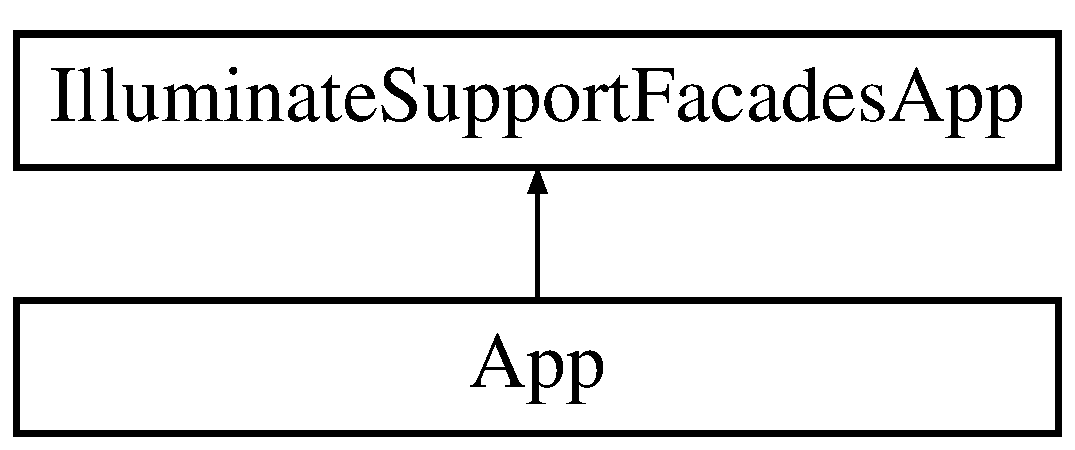
\includegraphics[height=2.000000cm]{class_app}
\end{center}
\end{figure}
\subsection*{Additional Inherited Members}


The documentation for this class was generated from the following file\+:\begin{DoxyCompactItemize}
\item 
\+\_\+ide\+\_\+helper.\+php\end{DoxyCompactItemize}

\hypertarget{class_illuminate_1_1_support_1_1_facades_1_1_artisan}{}\section{Illuminate\textbackslash{}Support\textbackslash{}Facades\textbackslash{}Artisan Class Reference}
\label{class_illuminate_1_1_support_1_1_facades_1_1_artisan}\index{Illuminate\textbackslash{}\+Support\textbackslash{}\+Facades\textbackslash{}\+Artisan@{Illuminate\textbackslash{}\+Support\textbackslash{}\+Facades\textbackslash{}\+Artisan}}
Inheritance diagram for Illuminate\textbackslash{}Support\textbackslash{}Facades\textbackslash{}Artisan\+:\begin{figure}[H]
\begin{center}
\leavevmode
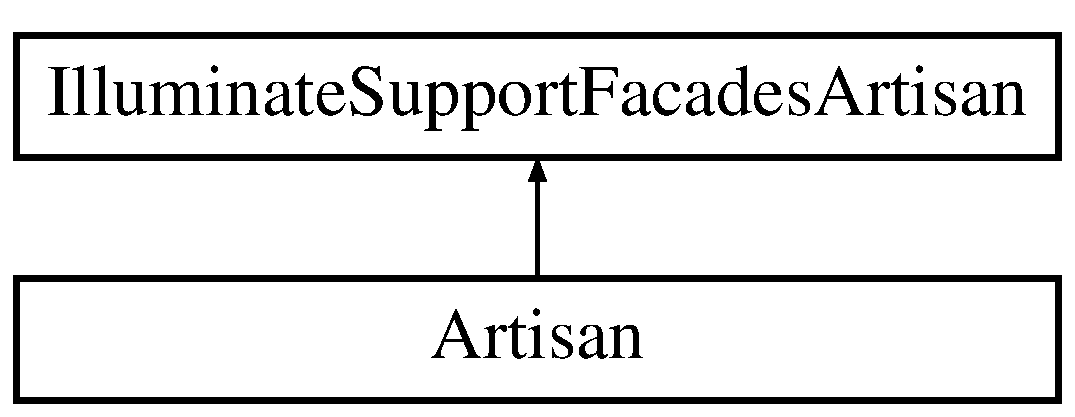
\includegraphics[height=2.000000cm]{class_illuminate_1_1_support_1_1_facades_1_1_artisan}
\end{center}
\end{figure}
\subsection*{Static Public Member Functions}
\begin{DoxyCompactItemize}
\item 
static \mbox{\hyperlink{class_illuminate_1_1_support_1_1_facades_1_1_artisan_a10a704e88a4a0f68ac198925f61b7495}{handle}} (\$input, \$\mbox{\hyperlink{class_illuminate_1_1_support_1_1_facades_1_1_artisan_a4de7cc04e2533e4f27c18239d831f5ad}{output}}=null)
\item 
static \mbox{\hyperlink{class_illuminate_1_1_support_1_1_facades_1_1_artisan_a8c902ee4dd700d08fd34ec6bcea9c064}{terminate}} (\$input, \$status)
\item 
static \mbox{\hyperlink{class_illuminate_1_1_support_1_1_facades_1_1_artisan_ac38347f7a2e06aa73d1a540921efdc27}{command}} (\$signature, \$callback)
\item 
static \mbox{\hyperlink{class_illuminate_1_1_support_1_1_facades_1_1_artisan_a8b26d2007bc40cec225f3b3954a8bc44}{register\+Command}} (\$\mbox{\hyperlink{class_illuminate_1_1_support_1_1_facades_1_1_artisan_ac38347f7a2e06aa73d1a540921efdc27}{command}})
\item 
static \mbox{\hyperlink{class_illuminate_1_1_support_1_1_facades_1_1_artisan_acbaec7ed7b40aee353ee70a69c78ea86}{call}} (\$\mbox{\hyperlink{class_illuminate_1_1_support_1_1_facades_1_1_artisan_ac38347f7a2e06aa73d1a540921efdc27}{command}}, \$parameters=array(), \$output\+Buffer=null)
\item 
static \mbox{\hyperlink{class_illuminate_1_1_support_1_1_facades_1_1_artisan_ac4bf1bf3446b86a77d55d2cf7ec1de5d}{queue}} (\$\mbox{\hyperlink{class_illuminate_1_1_support_1_1_facades_1_1_artisan_ac38347f7a2e06aa73d1a540921efdc27}{command}}, \$parameters=array())
\item 
static \mbox{\hyperlink{class_illuminate_1_1_support_1_1_facades_1_1_artisan_a87c2e2a664fba062b3fe585ff8997e2e}{all}} ()
\item 
static \mbox{\hyperlink{class_illuminate_1_1_support_1_1_facades_1_1_artisan_a4de7cc04e2533e4f27c18239d831f5ad}{output}} ()
\item 
static \mbox{\hyperlink{class_illuminate_1_1_support_1_1_facades_1_1_artisan_a08f421ef4a6faca630fb0c1ac505cc73}{bootstrap}} ()
\item 
static \mbox{\hyperlink{class_illuminate_1_1_support_1_1_facades_1_1_artisan_aea54192de87c7c3978fd552dc114e2ed}{set\+Artisan}} (\$artisan)
\end{DoxyCompactItemize}


\subsection{Member Function Documentation}
\mbox{\Hypertarget{class_illuminate_1_1_support_1_1_facades_1_1_artisan_a87c2e2a664fba062b3fe585ff8997e2e}\label{class_illuminate_1_1_support_1_1_facades_1_1_artisan_a87c2e2a664fba062b3fe585ff8997e2e}} 
\index{Illuminate\+::\+Support\+::\+Facades\+::\+Artisan@{Illuminate\+::\+Support\+::\+Facades\+::\+Artisan}!all@{all}}
\index{all@{all}!Illuminate\+::\+Support\+::\+Facades\+::\+Artisan@{Illuminate\+::\+Support\+::\+Facades\+::\+Artisan}}
\subsubsection{\texorpdfstring{all()}{all()}}
{\footnotesize\ttfamily static Illuminate\textbackslash{}\+Support\textbackslash{}\+Facades\textbackslash{}\+Artisan\+::all (\begin{DoxyParamCaption}{ }\end{DoxyParamCaption})\hspace{0.3cm}{\ttfamily [static]}}

Get all of the commands registered with the console.

\begin{DoxyReturn}{Returns}
array 
\end{DoxyReturn}
\mbox{\Hypertarget{class_illuminate_1_1_support_1_1_facades_1_1_artisan_a08f421ef4a6faca630fb0c1ac505cc73}\label{class_illuminate_1_1_support_1_1_facades_1_1_artisan_a08f421ef4a6faca630fb0c1ac505cc73}} 
\index{Illuminate\+::\+Support\+::\+Facades\+::\+Artisan@{Illuminate\+::\+Support\+::\+Facades\+::\+Artisan}!bootstrap@{bootstrap}}
\index{bootstrap@{bootstrap}!Illuminate\+::\+Support\+::\+Facades\+::\+Artisan@{Illuminate\+::\+Support\+::\+Facades\+::\+Artisan}}
\subsubsection{\texorpdfstring{bootstrap()}{bootstrap()}}
{\footnotesize\ttfamily static Illuminate\textbackslash{}\+Support\textbackslash{}\+Facades\textbackslash{}\+Artisan\+::bootstrap (\begin{DoxyParamCaption}{ }\end{DoxyParamCaption})\hspace{0.3cm}{\ttfamily [static]}}

Bootstrap the application for artisan commands.

\begin{DoxyReturn}{Returns}
void 
\end{DoxyReturn}
\mbox{\Hypertarget{class_illuminate_1_1_support_1_1_facades_1_1_artisan_acbaec7ed7b40aee353ee70a69c78ea86}\label{class_illuminate_1_1_support_1_1_facades_1_1_artisan_acbaec7ed7b40aee353ee70a69c78ea86}} 
\index{Illuminate\+::\+Support\+::\+Facades\+::\+Artisan@{Illuminate\+::\+Support\+::\+Facades\+::\+Artisan}!call@{call}}
\index{call@{call}!Illuminate\+::\+Support\+::\+Facades\+::\+Artisan@{Illuminate\+::\+Support\+::\+Facades\+::\+Artisan}}
\subsubsection{\texorpdfstring{call()}{call()}}
{\footnotesize\ttfamily static Illuminate\textbackslash{}\+Support\textbackslash{}\+Facades\textbackslash{}\+Artisan\+::call (\begin{DoxyParamCaption}\item[{}]{\$command,  }\item[{}]{\$parameters = {\ttfamily array()},  }\item[{}]{\$output\+Buffer = {\ttfamily null} }\end{DoxyParamCaption})\hspace{0.3cm}{\ttfamily [static]}}

Run an \mbox{\hyperlink{class_illuminate_1_1_support_1_1_facades_1_1_artisan}{Artisan}} console command by name.


\begin{DoxyParams}[1]{Parameters}
string & {\em \$command} & \\
\hline
array & {\em \$parameters} & \\
\hline
\textbackslash{}\+Symfony\textbackslash{}\+Component\textbackslash{}\+Console\textbackslash{}\+Output\textbackslash{}\+Output\+Interface & {\em \$output\+Buffer} & \\
\hline
\end{DoxyParams}
\begin{DoxyReturn}{Returns}
int 
\end{DoxyReturn}
\mbox{\Hypertarget{class_illuminate_1_1_support_1_1_facades_1_1_artisan_ac38347f7a2e06aa73d1a540921efdc27}\label{class_illuminate_1_1_support_1_1_facades_1_1_artisan_ac38347f7a2e06aa73d1a540921efdc27}} 
\index{Illuminate\+::\+Support\+::\+Facades\+::\+Artisan@{Illuminate\+::\+Support\+::\+Facades\+::\+Artisan}!command@{command}}
\index{command@{command}!Illuminate\+::\+Support\+::\+Facades\+::\+Artisan@{Illuminate\+::\+Support\+::\+Facades\+::\+Artisan}}
\subsubsection{\texorpdfstring{command()}{command()}}
{\footnotesize\ttfamily static Illuminate\textbackslash{}\+Support\textbackslash{}\+Facades\textbackslash{}\+Artisan\+::command (\begin{DoxyParamCaption}\item[{}]{\$signature,  }\item[{}]{\$callback }\end{DoxyParamCaption})\hspace{0.3cm}{\ttfamily [static]}}

Register a Closure based command with the application.


\begin{DoxyParams}[1]{Parameters}
string & {\em \$signature} & \\
\hline
\textbackslash{}\+Closure & {\em \$callback} & \\
\hline
\end{DoxyParams}
\begin{DoxyReturn}{Returns}

\end{DoxyReturn}
\mbox{\Hypertarget{class_illuminate_1_1_support_1_1_facades_1_1_artisan_a10a704e88a4a0f68ac198925f61b7495}\label{class_illuminate_1_1_support_1_1_facades_1_1_artisan_a10a704e88a4a0f68ac198925f61b7495}} 
\index{Illuminate\+::\+Support\+::\+Facades\+::\+Artisan@{Illuminate\+::\+Support\+::\+Facades\+::\+Artisan}!handle@{handle}}
\index{handle@{handle}!Illuminate\+::\+Support\+::\+Facades\+::\+Artisan@{Illuminate\+::\+Support\+::\+Facades\+::\+Artisan}}
\subsubsection{\texorpdfstring{handle()}{handle()}}
{\footnotesize\ttfamily static Illuminate\textbackslash{}\+Support\textbackslash{}\+Facades\textbackslash{}\+Artisan\+::handle (\begin{DoxyParamCaption}\item[{}]{\$input,  }\item[{}]{\$output = {\ttfamily null} }\end{DoxyParamCaption})\hspace{0.3cm}{\ttfamily [static]}}

Run the console application.


\begin{DoxyParams}[1]{Parameters}
\textbackslash{}\+Symfony\textbackslash{}\+Component\textbackslash{}\+Console\textbackslash{}\+Input\textbackslash{}\+Input\+Interface & {\em \$input} & \\
\hline
\textbackslash{}\+Symfony\textbackslash{}\+Component\textbackslash{}\+Console\textbackslash{}\+Output\textbackslash{}\+Output\+Interface & {\em \$output} & \\
\hline
\end{DoxyParams}
\begin{DoxyReturn}{Returns}
int 
\end{DoxyReturn}
\mbox{\Hypertarget{class_illuminate_1_1_support_1_1_facades_1_1_artisan_a4de7cc04e2533e4f27c18239d831f5ad}\label{class_illuminate_1_1_support_1_1_facades_1_1_artisan_a4de7cc04e2533e4f27c18239d831f5ad}} 
\index{Illuminate\+::\+Support\+::\+Facades\+::\+Artisan@{Illuminate\+::\+Support\+::\+Facades\+::\+Artisan}!output@{output}}
\index{output@{output}!Illuminate\+::\+Support\+::\+Facades\+::\+Artisan@{Illuminate\+::\+Support\+::\+Facades\+::\+Artisan}}
\subsubsection{\texorpdfstring{output()}{output()}}
{\footnotesize\ttfamily static Illuminate\textbackslash{}\+Support\textbackslash{}\+Facades\textbackslash{}\+Artisan\+::output (\begin{DoxyParamCaption}{ }\end{DoxyParamCaption})\hspace{0.3cm}{\ttfamily [static]}}

Get the output for the last run command.

\begin{DoxyReturn}{Returns}
string 
\end{DoxyReturn}
\mbox{\Hypertarget{class_illuminate_1_1_support_1_1_facades_1_1_artisan_ac4bf1bf3446b86a77d55d2cf7ec1de5d}\label{class_illuminate_1_1_support_1_1_facades_1_1_artisan_ac4bf1bf3446b86a77d55d2cf7ec1de5d}} 
\index{Illuminate\+::\+Support\+::\+Facades\+::\+Artisan@{Illuminate\+::\+Support\+::\+Facades\+::\+Artisan}!queue@{queue}}
\index{queue@{queue}!Illuminate\+::\+Support\+::\+Facades\+::\+Artisan@{Illuminate\+::\+Support\+::\+Facades\+::\+Artisan}}
\subsubsection{\texorpdfstring{queue()}{queue()}}
{\footnotesize\ttfamily static Illuminate\textbackslash{}\+Support\textbackslash{}\+Facades\textbackslash{}\+Artisan\+::queue (\begin{DoxyParamCaption}\item[{}]{\$command,  }\item[{}]{\$parameters = {\ttfamily array()} }\end{DoxyParamCaption})\hspace{0.3cm}{\ttfamily [static]}}

\mbox{\hyperlink{class_illuminate_1_1_support_1_1_facades_1_1_queue}{Queue}} the given console command.


\begin{DoxyParams}[1]{Parameters}
string & {\em \$command} & \\
\hline
array & {\em \$parameters} & \\
\hline
\end{DoxyParams}
\begin{DoxyReturn}{Returns}

\end{DoxyReturn}
\mbox{\Hypertarget{class_illuminate_1_1_support_1_1_facades_1_1_artisan_a8b26d2007bc40cec225f3b3954a8bc44}\label{class_illuminate_1_1_support_1_1_facades_1_1_artisan_a8b26d2007bc40cec225f3b3954a8bc44}} 
\index{Illuminate\+::\+Support\+::\+Facades\+::\+Artisan@{Illuminate\+::\+Support\+::\+Facades\+::\+Artisan}!register\+Command@{register\+Command}}
\index{register\+Command@{register\+Command}!Illuminate\+::\+Support\+::\+Facades\+::\+Artisan@{Illuminate\+::\+Support\+::\+Facades\+::\+Artisan}}
\subsubsection{\texorpdfstring{register\+Command()}{registerCommand()}}
{\footnotesize\ttfamily static Illuminate\textbackslash{}\+Support\textbackslash{}\+Facades\textbackslash{}\+Artisan\+::register\+Command (\begin{DoxyParamCaption}\item[{}]{\$command }\end{DoxyParamCaption})\hspace{0.3cm}{\ttfamily [static]}}

Register the given command with the console application.


\begin{DoxyParams}[1]{Parameters}
\textbackslash{}\+Symfony\textbackslash{}\+Component\textbackslash{}\+Console\textbackslash{}\+Command\textbackslash{}\+Command & {\em \$command} & \\
\hline
\end{DoxyParams}
\begin{DoxyReturn}{Returns}
void 
\end{DoxyReturn}
\mbox{\Hypertarget{class_illuminate_1_1_support_1_1_facades_1_1_artisan_aea54192de87c7c3978fd552dc114e2ed}\label{class_illuminate_1_1_support_1_1_facades_1_1_artisan_aea54192de87c7c3978fd552dc114e2ed}} 
\index{Illuminate\+::\+Support\+::\+Facades\+::\+Artisan@{Illuminate\+::\+Support\+::\+Facades\+::\+Artisan}!set\+Artisan@{set\+Artisan}}
\index{set\+Artisan@{set\+Artisan}!Illuminate\+::\+Support\+::\+Facades\+::\+Artisan@{Illuminate\+::\+Support\+::\+Facades\+::\+Artisan}}
\subsubsection{\texorpdfstring{set\+Artisan()}{setArtisan()}}
{\footnotesize\ttfamily static Illuminate\textbackslash{}\+Support\textbackslash{}\+Facades\textbackslash{}\+Artisan\+::set\+Artisan (\begin{DoxyParamCaption}\item[{}]{\$artisan }\end{DoxyParamCaption})\hspace{0.3cm}{\ttfamily [static]}}

Set the \mbox{\hyperlink{class_illuminate_1_1_support_1_1_facades_1_1_artisan}{Artisan}} application instance.


\begin{DoxyParams}[1]{Parameters}
\textbackslash{}\+Illuminate\textbackslash{}\+Console\textbackslash{}\+Application & {\em \$artisan} & \\
\hline
\end{DoxyParams}
\begin{DoxyReturn}{Returns}
void 
\end{DoxyReturn}
\mbox{\Hypertarget{class_illuminate_1_1_support_1_1_facades_1_1_artisan_a8c902ee4dd700d08fd34ec6bcea9c064}\label{class_illuminate_1_1_support_1_1_facades_1_1_artisan_a8c902ee4dd700d08fd34ec6bcea9c064}} 
\index{Illuminate\+::\+Support\+::\+Facades\+::\+Artisan@{Illuminate\+::\+Support\+::\+Facades\+::\+Artisan}!terminate@{terminate}}
\index{terminate@{terminate}!Illuminate\+::\+Support\+::\+Facades\+::\+Artisan@{Illuminate\+::\+Support\+::\+Facades\+::\+Artisan}}
\subsubsection{\texorpdfstring{terminate()}{terminate()}}
{\footnotesize\ttfamily static Illuminate\textbackslash{}\+Support\textbackslash{}\+Facades\textbackslash{}\+Artisan\+::terminate (\begin{DoxyParamCaption}\item[{}]{\$input,  }\item[{}]{\$status }\end{DoxyParamCaption})\hspace{0.3cm}{\ttfamily [static]}}

Terminate the application.


\begin{DoxyParams}[1]{Parameters}
\textbackslash{}\+Symfony\textbackslash{}\+Component\textbackslash{}\+Console\textbackslash{}\+Input\textbackslash{}\+Input\+Interface & {\em \$input} & \\
\hline
int & {\em \$status} & \\
\hline
\end{DoxyParams}
\begin{DoxyReturn}{Returns}
void 
\end{DoxyReturn}


The documentation for this class was generated from the following file\+:\begin{DoxyCompactItemize}
\item 
\+\_\+ide\+\_\+helper.\+php\end{DoxyCompactItemize}

\hypertarget{class_artisan}{}\section{Artisan Class Reference}
\label{class_artisan}\index{Artisan@{Artisan}}
Inheritance diagram for Artisan\+:\begin{figure}[H]
\begin{center}
\leavevmode
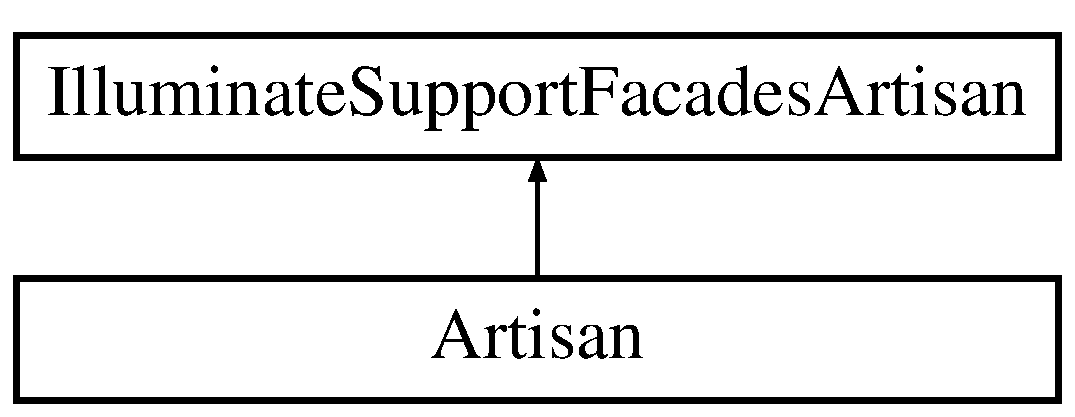
\includegraphics[height=2.000000cm]{class_artisan}
\end{center}
\end{figure}
\subsection*{Additional Inherited Members}


The documentation for this class was generated from the following file\+:\begin{DoxyCompactItemize}
\item 
\+\_\+ide\+\_\+helper.\+php\end{DoxyCompactItemize}

\hypertarget{class_auth}{}\section{Auth Class Reference}
\label{class_auth}\index{Auth@{Auth}}
Inheritance diagram for Auth\+:\begin{figure}[H]
\begin{center}
\leavevmode
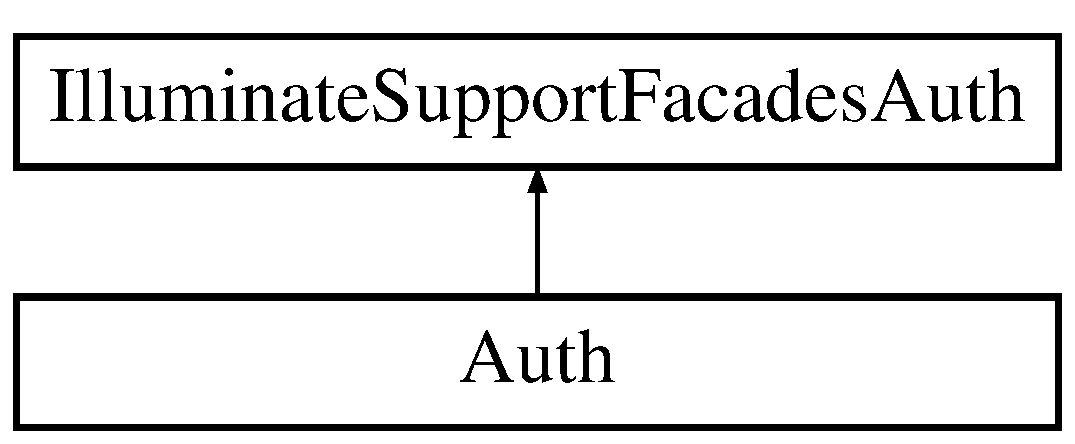
\includegraphics[height=2.000000cm]{class_auth}
\end{center}
\end{figure}
\subsection*{Additional Inherited Members}


The documentation for this class was generated from the following file\+:\begin{DoxyCompactItemize}
\item 
\+\_\+ide\+\_\+helper.\+php\end{DoxyCompactItemize}

\hypertarget{class_illuminate_1_1_support_1_1_facades_1_1_auth}{}\section{Illuminate\textbackslash{}Support\textbackslash{}Facades\textbackslash{}Auth Class Reference}
\label{class_illuminate_1_1_support_1_1_facades_1_1_auth}\index{Illuminate\textbackslash{}\+Support\textbackslash{}\+Facades\textbackslash{}\+Auth@{Illuminate\textbackslash{}\+Support\textbackslash{}\+Facades\textbackslash{}\+Auth}}
Inheritance diagram for Illuminate\textbackslash{}Support\textbackslash{}Facades\textbackslash{}Auth\+:\begin{figure}[H]
\begin{center}
\leavevmode
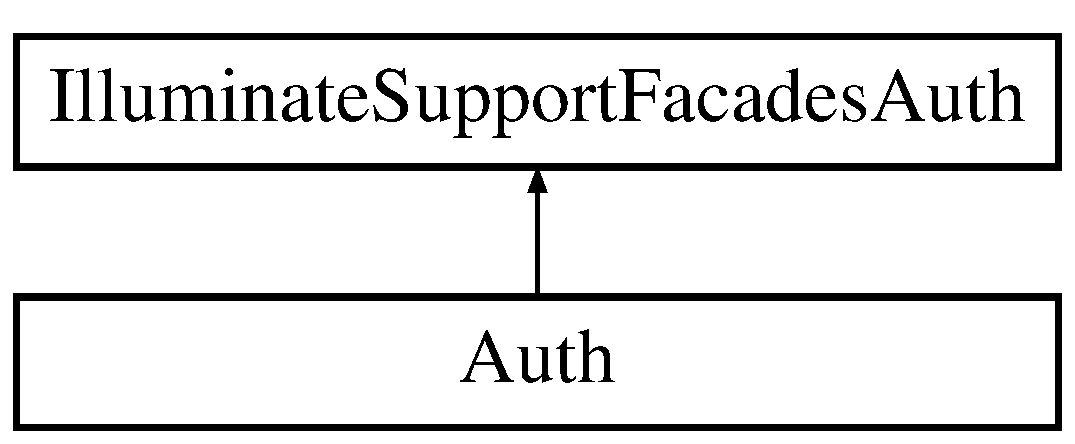
\includegraphics[height=2.000000cm]{class_illuminate_1_1_support_1_1_facades_1_1_auth}
\end{center}
\end{figure}
\subsection*{Static Public Member Functions}
\begin{DoxyCompactItemize}
\item 
static \mbox{\hyperlink{class_illuminate_1_1_support_1_1_facades_1_1_auth_a432fde79e22091b6140b1fdbc725a72d}{guard}} (\$name=null)
\item 
static \mbox{\hyperlink{class_illuminate_1_1_support_1_1_facades_1_1_auth_a62a5d99a2d3d429c0f268824ca653803}{create\+Session\+Driver}} (\$name, \$config)
\item 
static \mbox{\hyperlink{class_illuminate_1_1_support_1_1_facades_1_1_auth_aafc443ec8004cdce83d728e6f04f8994}{create\+Token\+Driver}} (\$name, \$config)
\item 
static \mbox{\hyperlink{class_illuminate_1_1_support_1_1_facades_1_1_auth_a28c2308e161fd8146ed3d2e8481827d0}{get\+Default\+Driver}} ()
\item 
static \mbox{\hyperlink{class_illuminate_1_1_support_1_1_facades_1_1_auth_acc225c4397c62a6f93d9bd87bba44562}{should\+Use}} (\$name)
\item 
static \mbox{\hyperlink{class_illuminate_1_1_support_1_1_facades_1_1_auth_ae76bb55b5f629f397cc1e4e6c1c7b214}{set\+Default\+Driver}} (\$name)
\item 
static \mbox{\hyperlink{class_illuminate_1_1_support_1_1_facades_1_1_auth_a6c74f6505618b87ab69949b662fba9b9}{via\+Request}} (\$driver, \$callback)
\item 
static \mbox{\hyperlink{class_illuminate_1_1_support_1_1_facades_1_1_auth_ab6601a8ada37b3aaaab8700de51eb523}{user\+Resolver}} ()
\item 
static \mbox{\hyperlink{class_illuminate_1_1_support_1_1_facades_1_1_auth_af5d4285e6f94d28c07f9ab9f7077df5a}{resolve\+Users\+Using}} (\$\mbox{\hyperlink{class_illuminate_1_1_support_1_1_facades_1_1_auth_ab6601a8ada37b3aaaab8700de51eb523}{user\+Resolver}})
\item 
static \mbox{\hyperlink{class_illuminate_1_1_support_1_1_facades_1_1_auth_ad6fdb08c1e3db9081087ec888f3c0193}{extend}} (\$driver, \$callback)
\item 
static \mbox{\hyperlink{class_illuminate_1_1_support_1_1_facades_1_1_auth_abf132c9b8d5ccce533211625ec83dc35}{provider}} (\$name, \$callback)
\item 
static \mbox{\hyperlink{class_illuminate_1_1_support_1_1_facades_1_1_auth_afdd867755aae03ffd16c73de0daff938}{create\+User\+Provider}} (\$\mbox{\hyperlink{class_illuminate_1_1_support_1_1_facades_1_1_auth_abf132c9b8d5ccce533211625ec83dc35}{provider}}=null)
\item 
static \mbox{\hyperlink{class_illuminate_1_1_support_1_1_facades_1_1_auth_a2b44e6e6ceebe194082a5ffe7db7aaaf}{get\+Default\+User\+Provider}} ()
\item 
static \mbox{\hyperlink{class_illuminate_1_1_support_1_1_facades_1_1_auth_a0e25fe7a8574e495c4e48ee60813f249}{user}} ()
\item 
static \mbox{\hyperlink{class_illuminate_1_1_support_1_1_facades_1_1_auth_ab98365becdcd81b76d4be5aaa6971a05}{id}} ()
\item 
static \mbox{\hyperlink{class_illuminate_1_1_support_1_1_facades_1_1_auth_a63d7ab8bd8f2fd996d828789d339566a}{once}} (\$credentials=array())
\item 
static \mbox{\hyperlink{class_illuminate_1_1_support_1_1_facades_1_1_auth_a91dc83481e1323700b6d3d69ce944f05}{once\+Using\+Id}} (\$\mbox{\hyperlink{class_illuminate_1_1_support_1_1_facades_1_1_auth_ab98365becdcd81b76d4be5aaa6971a05}{id}})
\item 
static \mbox{\hyperlink{class_illuminate_1_1_support_1_1_facades_1_1_auth_a3bae01dfeecf84ab4ab06d46ae4214f7}{validate}} (\$credentials=array())
\item 
static \mbox{\hyperlink{class_illuminate_1_1_support_1_1_facades_1_1_auth_af8f2ff30a669fd33795db2d7947aa4bd}{basic}} (\$field=\textquotesingle{}email\textquotesingle{}, \$extra\+Conditions=array())
\item 
static \mbox{\hyperlink{class_illuminate_1_1_support_1_1_facades_1_1_auth_a655de6df527a9ea10578d8b273166f22}{once\+Basic}} (\$field=\textquotesingle{}email\textquotesingle{}, \$extra\+Conditions=array())
\item 
static \mbox{\hyperlink{class_illuminate_1_1_support_1_1_facades_1_1_auth_aaae9451317576aa597277bac1aa2331d}{attempt}} (\$credentials=array(), \$remember=false)
\item 
static \mbox{\hyperlink{class_illuminate_1_1_support_1_1_facades_1_1_auth_a96b66e55dc3ced8f3c89e77171f01f4b}{login\+Using\+Id}} (\$\mbox{\hyperlink{class_illuminate_1_1_support_1_1_facades_1_1_auth_ab98365becdcd81b76d4be5aaa6971a05}{id}}, \$remember=false)
\item 
static \mbox{\hyperlink{class_illuminate_1_1_support_1_1_facades_1_1_auth_aeef81e7eab1a76858dfa1b5e2d251bf0}{login}} (\$\mbox{\hyperlink{class_illuminate_1_1_support_1_1_facades_1_1_auth_a0e25fe7a8574e495c4e48ee60813f249}{user}}, \$remember=false)
\item 
static \mbox{\hyperlink{class_illuminate_1_1_support_1_1_facades_1_1_auth_a53e1351df33655142a42751eba04297b}{logout}} ()
\item 
static \mbox{\hyperlink{class_illuminate_1_1_support_1_1_facades_1_1_auth_a40f114974e5275c1151439c6e5b125a2}{attempting}} (\$callback)
\item 
static \mbox{\hyperlink{class_illuminate_1_1_support_1_1_facades_1_1_auth_a9894e0a62cb7c0f15bdb3f864ee907d0}{get\+Last\+Attempted}} ()
\item 
static \mbox{\hyperlink{class_illuminate_1_1_support_1_1_facades_1_1_auth_a065ace7a83e0b21199870acf32eca1ba}{get\+Name}} ()
\item 
static \mbox{\hyperlink{class_illuminate_1_1_support_1_1_facades_1_1_auth_a21da3c773fb2d59228c84cac75344034}{get\+Recaller\+Name}} ()
\item 
static \mbox{\hyperlink{class_illuminate_1_1_support_1_1_facades_1_1_auth_a007b8696ba0250c38255e1bd3b23dbd5}{via\+Remember}} ()
\item 
static \mbox{\hyperlink{class_illuminate_1_1_support_1_1_facades_1_1_auth_a33a191c912e59b497c73cf3b5c881f5e}{get\+Cookie\+Jar}} ()
\item 
static \mbox{\hyperlink{class_illuminate_1_1_support_1_1_facades_1_1_auth_a89cb1bc85a383e7453d7b940651a4a04}{set\+Cookie\+Jar}} (\$cookie)
\item 
static \mbox{\hyperlink{class_illuminate_1_1_support_1_1_facades_1_1_auth_a5085d618634062b5794d73702d2e58cc}{get\+Dispatcher}} ()
\item 
static \mbox{\hyperlink{class_illuminate_1_1_support_1_1_facades_1_1_auth_ac8c611f42d922a4825347a7f92910922}{set\+Dispatcher}} (\$events)
\item 
static \mbox{\hyperlink{class_illuminate_1_1_support_1_1_facades_1_1_auth_aff8249330f0e005703f568c33a557566}{get\+Session}} ()
\item 
static \mbox{\hyperlink{class_illuminate_1_1_support_1_1_facades_1_1_auth_a32bd05e2dde1227b3a8a32613cbe1bf6}{get\+User}} ()
\item 
static \mbox{\hyperlink{class_illuminate_1_1_support_1_1_facades_1_1_auth_aef0606291d204ec7554b9afab827ceb7}{set\+User}} (\$\mbox{\hyperlink{class_illuminate_1_1_support_1_1_facades_1_1_auth_a0e25fe7a8574e495c4e48ee60813f249}{user}})
\item 
static \mbox{\hyperlink{class_illuminate_1_1_support_1_1_facades_1_1_auth_af626e26e10b0d8e17a624c8db984a65c}{get\+Request}} ()
\item 
static \mbox{\hyperlink{class_illuminate_1_1_support_1_1_facades_1_1_auth_ae0cb110e3c059aae5571e6ed4b11bd3b}{set\+Request}} (\$request)
\item 
static \mbox{\hyperlink{class_illuminate_1_1_support_1_1_facades_1_1_auth_aa4b00209ad83c9a457af1cf9c0eb98a9}{authenticate}} ()
\item 
static \mbox{\hyperlink{class_illuminate_1_1_support_1_1_facades_1_1_auth_a4d5eba4e6245d756cd3eb807cadd2e2a}{check}} ()
\item 
static \mbox{\hyperlink{class_illuminate_1_1_support_1_1_facades_1_1_auth_a4aef095d6c9b7f60b7b1384d4064eb55}{guest}} ()
\item 
static \mbox{\hyperlink{class_illuminate_1_1_support_1_1_facades_1_1_auth_a0e62552b70450b179a28f6e45d7cb937}{get\+Provider}} ()
\item 
static \mbox{\hyperlink{class_illuminate_1_1_support_1_1_facades_1_1_auth_a8c2ecd65aa1a1607a35519b566bd66da}{set\+Provider}} (\$\mbox{\hyperlink{class_illuminate_1_1_support_1_1_facades_1_1_auth_abf132c9b8d5ccce533211625ec83dc35}{provider}})
\item 
static \mbox{\hyperlink{class_illuminate_1_1_support_1_1_facades_1_1_auth_aa79d00741e5434bcb76731a02ffb361a}{macro}} (\$name, \$macro)
\item 
static \mbox{\hyperlink{class_illuminate_1_1_support_1_1_facades_1_1_auth_a5b3b067862dcf209c346a45f0addcf4d}{mixin}} (\$mixin)
\item 
static \mbox{\hyperlink{class_illuminate_1_1_support_1_1_facades_1_1_auth_a9ec6110e79e885017d5e4d3ad20392e1}{has\+Macro}} (\$name)
\end{DoxyCompactItemize}


\subsection{Member Function Documentation}
\mbox{\Hypertarget{class_illuminate_1_1_support_1_1_facades_1_1_auth_aaae9451317576aa597277bac1aa2331d}\label{class_illuminate_1_1_support_1_1_facades_1_1_auth_aaae9451317576aa597277bac1aa2331d}} 
\index{Illuminate\+::\+Support\+::\+Facades\+::\+Auth@{Illuminate\+::\+Support\+::\+Facades\+::\+Auth}!attempt@{attempt}}
\index{attempt@{attempt}!Illuminate\+::\+Support\+::\+Facades\+::\+Auth@{Illuminate\+::\+Support\+::\+Facades\+::\+Auth}}
\subsubsection{\texorpdfstring{attempt()}{attempt()}}
{\footnotesize\ttfamily static Illuminate\textbackslash{}\+Support\textbackslash{}\+Facades\textbackslash{}\+Auth\+::attempt (\begin{DoxyParamCaption}\item[{}]{\$credentials = {\ttfamily array()},  }\item[{}]{\$remember = {\ttfamily false} }\end{DoxyParamCaption})\hspace{0.3cm}{\ttfamily [static]}}

Attempt to authenticate a user using the given credentials.


\begin{DoxyParams}[1]{Parameters}
array & {\em \$credentials} & \\
\hline
bool & {\em \$remember} & \\
\hline
\end{DoxyParams}
\begin{DoxyReturn}{Returns}
bool 
\end{DoxyReturn}
\mbox{\Hypertarget{class_illuminate_1_1_support_1_1_facades_1_1_auth_a40f114974e5275c1151439c6e5b125a2}\label{class_illuminate_1_1_support_1_1_facades_1_1_auth_a40f114974e5275c1151439c6e5b125a2}} 
\index{Illuminate\+::\+Support\+::\+Facades\+::\+Auth@{Illuminate\+::\+Support\+::\+Facades\+::\+Auth}!attempting@{attempting}}
\index{attempting@{attempting}!Illuminate\+::\+Support\+::\+Facades\+::\+Auth@{Illuminate\+::\+Support\+::\+Facades\+::\+Auth}}
\subsubsection{\texorpdfstring{attempting()}{attempting()}}
{\footnotesize\ttfamily static Illuminate\textbackslash{}\+Support\textbackslash{}\+Facades\textbackslash{}\+Auth\+::attempting (\begin{DoxyParamCaption}\item[{}]{\$callback }\end{DoxyParamCaption})\hspace{0.3cm}{\ttfamily [static]}}

Register an authentication attempt event listener.


\begin{DoxyParams}[1]{Parameters}
mixed & {\em \$callback} & \\
\hline
\end{DoxyParams}
\begin{DoxyReturn}{Returns}
void 
\end{DoxyReturn}
\mbox{\Hypertarget{class_illuminate_1_1_support_1_1_facades_1_1_auth_aa4b00209ad83c9a457af1cf9c0eb98a9}\label{class_illuminate_1_1_support_1_1_facades_1_1_auth_aa4b00209ad83c9a457af1cf9c0eb98a9}} 
\index{Illuminate\+::\+Support\+::\+Facades\+::\+Auth@{Illuminate\+::\+Support\+::\+Facades\+::\+Auth}!authenticate@{authenticate}}
\index{authenticate@{authenticate}!Illuminate\+::\+Support\+::\+Facades\+::\+Auth@{Illuminate\+::\+Support\+::\+Facades\+::\+Auth}}
\subsubsection{\texorpdfstring{authenticate()}{authenticate()}}
{\footnotesize\ttfamily static Illuminate\textbackslash{}\+Support\textbackslash{}\+Facades\textbackslash{}\+Auth\+::authenticate (\begin{DoxyParamCaption}{ }\end{DoxyParamCaption})\hspace{0.3cm}{\ttfamily [static]}}

Determine if the current user is authenticated.

\begin{DoxyReturn}{Returns}

\end{DoxyReturn}

\begin{DoxyExceptions}{Exceptions}
{\em } & \\
\hline
\end{DoxyExceptions}
\mbox{\Hypertarget{class_illuminate_1_1_support_1_1_facades_1_1_auth_af8f2ff30a669fd33795db2d7947aa4bd}\label{class_illuminate_1_1_support_1_1_facades_1_1_auth_af8f2ff30a669fd33795db2d7947aa4bd}} 
\index{Illuminate\+::\+Support\+::\+Facades\+::\+Auth@{Illuminate\+::\+Support\+::\+Facades\+::\+Auth}!basic@{basic}}
\index{basic@{basic}!Illuminate\+::\+Support\+::\+Facades\+::\+Auth@{Illuminate\+::\+Support\+::\+Facades\+::\+Auth}}
\subsubsection{\texorpdfstring{basic()}{basic()}}
{\footnotesize\ttfamily static Illuminate\textbackslash{}\+Support\textbackslash{}\+Facades\textbackslash{}\+Auth\+::basic (\begin{DoxyParamCaption}\item[{}]{\$field = {\ttfamily \textquotesingle{}email\textquotesingle{}},  }\item[{}]{\$extra\+Conditions = {\ttfamily array()} }\end{DoxyParamCaption})\hspace{0.3cm}{\ttfamily [static]}}

Attempt to authenticate using H\+T\+TP Basic \mbox{\hyperlink{class_illuminate_1_1_support_1_1_facades_1_1_auth}{Auth}}.


\begin{DoxyParams}[1]{Parameters}
string & {\em \$field} & \\
\hline
array & {\em \$extra\+Conditions} & \\
\hline
\end{DoxyParams}
\begin{DoxyReturn}{Returns}
$\vert$null 
\end{DoxyReturn}
\mbox{\Hypertarget{class_illuminate_1_1_support_1_1_facades_1_1_auth_a4d5eba4e6245d756cd3eb807cadd2e2a}\label{class_illuminate_1_1_support_1_1_facades_1_1_auth_a4d5eba4e6245d756cd3eb807cadd2e2a}} 
\index{Illuminate\+::\+Support\+::\+Facades\+::\+Auth@{Illuminate\+::\+Support\+::\+Facades\+::\+Auth}!check@{check}}
\index{check@{check}!Illuminate\+::\+Support\+::\+Facades\+::\+Auth@{Illuminate\+::\+Support\+::\+Facades\+::\+Auth}}
\subsubsection{\texorpdfstring{check()}{check()}}
{\footnotesize\ttfamily static Illuminate\textbackslash{}\+Support\textbackslash{}\+Facades\textbackslash{}\+Auth\+::check (\begin{DoxyParamCaption}{ }\end{DoxyParamCaption})\hspace{0.3cm}{\ttfamily [static]}}

Determine if the current user is authenticated.

\begin{DoxyReturn}{Returns}
bool 
\end{DoxyReturn}
\mbox{\Hypertarget{class_illuminate_1_1_support_1_1_facades_1_1_auth_a62a5d99a2d3d429c0f268824ca653803}\label{class_illuminate_1_1_support_1_1_facades_1_1_auth_a62a5d99a2d3d429c0f268824ca653803}} 
\index{Illuminate\+::\+Support\+::\+Facades\+::\+Auth@{Illuminate\+::\+Support\+::\+Facades\+::\+Auth}!create\+Session\+Driver@{create\+Session\+Driver}}
\index{create\+Session\+Driver@{create\+Session\+Driver}!Illuminate\+::\+Support\+::\+Facades\+::\+Auth@{Illuminate\+::\+Support\+::\+Facades\+::\+Auth}}
\subsubsection{\texorpdfstring{create\+Session\+Driver()}{createSessionDriver()}}
{\footnotesize\ttfamily static Illuminate\textbackslash{}\+Support\textbackslash{}\+Facades\textbackslash{}\+Auth\+::create\+Session\+Driver (\begin{DoxyParamCaption}\item[{}]{\$name,  }\item[{}]{\$config }\end{DoxyParamCaption})\hspace{0.3cm}{\ttfamily [static]}}

Create a session based authentication guard.


\begin{DoxyParams}[1]{Parameters}
string & {\em \$name} & \\
\hline
array & {\em \$config} & \\
\hline
\end{DoxyParams}
\begin{DoxyReturn}{Returns}

\end{DoxyReturn}
\mbox{\Hypertarget{class_illuminate_1_1_support_1_1_facades_1_1_auth_aafc443ec8004cdce83d728e6f04f8994}\label{class_illuminate_1_1_support_1_1_facades_1_1_auth_aafc443ec8004cdce83d728e6f04f8994}} 
\index{Illuminate\+::\+Support\+::\+Facades\+::\+Auth@{Illuminate\+::\+Support\+::\+Facades\+::\+Auth}!create\+Token\+Driver@{create\+Token\+Driver}}
\index{create\+Token\+Driver@{create\+Token\+Driver}!Illuminate\+::\+Support\+::\+Facades\+::\+Auth@{Illuminate\+::\+Support\+::\+Facades\+::\+Auth}}
\subsubsection{\texorpdfstring{create\+Token\+Driver()}{createTokenDriver()}}
{\footnotesize\ttfamily static Illuminate\textbackslash{}\+Support\textbackslash{}\+Facades\textbackslash{}\+Auth\+::create\+Token\+Driver (\begin{DoxyParamCaption}\item[{}]{\$name,  }\item[{}]{\$config }\end{DoxyParamCaption})\hspace{0.3cm}{\ttfamily [static]}}

Create a token based authentication guard.


\begin{DoxyParams}[1]{Parameters}
string & {\em \$name} & \\
\hline
array & {\em \$config} & \\
\hline
\end{DoxyParams}
\begin{DoxyReturn}{Returns}

\end{DoxyReturn}
\mbox{\Hypertarget{class_illuminate_1_1_support_1_1_facades_1_1_auth_afdd867755aae03ffd16c73de0daff938}\label{class_illuminate_1_1_support_1_1_facades_1_1_auth_afdd867755aae03ffd16c73de0daff938}} 
\index{Illuminate\+::\+Support\+::\+Facades\+::\+Auth@{Illuminate\+::\+Support\+::\+Facades\+::\+Auth}!create\+User\+Provider@{create\+User\+Provider}}
\index{create\+User\+Provider@{create\+User\+Provider}!Illuminate\+::\+Support\+::\+Facades\+::\+Auth@{Illuminate\+::\+Support\+::\+Facades\+::\+Auth}}
\subsubsection{\texorpdfstring{create\+User\+Provider()}{createUserProvider()}}
{\footnotesize\ttfamily static Illuminate\textbackslash{}\+Support\textbackslash{}\+Facades\textbackslash{}\+Auth\+::create\+User\+Provider (\begin{DoxyParamCaption}\item[{}]{\$provider = {\ttfamily null} }\end{DoxyParamCaption})\hspace{0.3cm}{\ttfamily [static]}}

Create the user provider implementation for the driver.


\begin{DoxyParams}[1]{Parameters}
string | null & {\em \$provider} & \\
\hline
\end{DoxyParams}
\begin{DoxyReturn}{Returns}
$\vert$null 
\end{DoxyReturn}

\begin{DoxyExceptions}{Exceptions}
{\em } & \\
\hline
\end{DoxyExceptions}
\mbox{\Hypertarget{class_illuminate_1_1_support_1_1_facades_1_1_auth_ad6fdb08c1e3db9081087ec888f3c0193}\label{class_illuminate_1_1_support_1_1_facades_1_1_auth_ad6fdb08c1e3db9081087ec888f3c0193}} 
\index{Illuminate\+::\+Support\+::\+Facades\+::\+Auth@{Illuminate\+::\+Support\+::\+Facades\+::\+Auth}!extend@{extend}}
\index{extend@{extend}!Illuminate\+::\+Support\+::\+Facades\+::\+Auth@{Illuminate\+::\+Support\+::\+Facades\+::\+Auth}}
\subsubsection{\texorpdfstring{extend()}{extend()}}
{\footnotesize\ttfamily static Illuminate\textbackslash{}\+Support\textbackslash{}\+Facades\textbackslash{}\+Auth\+::extend (\begin{DoxyParamCaption}\item[{}]{\$driver,  }\item[{}]{\$callback }\end{DoxyParamCaption})\hspace{0.3cm}{\ttfamily [static]}}

Register a custom driver creator Closure.


\begin{DoxyParams}[1]{Parameters}
string & {\em \$driver} & \\
\hline
\textbackslash{}\+Closure & {\em \$callback} & \\
\hline
\end{DoxyParams}
\begin{DoxyReturn}{Returns}
\$this 
\end{DoxyReturn}
\mbox{\Hypertarget{class_illuminate_1_1_support_1_1_facades_1_1_auth_a33a191c912e59b497c73cf3b5c881f5e}\label{class_illuminate_1_1_support_1_1_facades_1_1_auth_a33a191c912e59b497c73cf3b5c881f5e}} 
\index{Illuminate\+::\+Support\+::\+Facades\+::\+Auth@{Illuminate\+::\+Support\+::\+Facades\+::\+Auth}!get\+Cookie\+Jar@{get\+Cookie\+Jar}}
\index{get\+Cookie\+Jar@{get\+Cookie\+Jar}!Illuminate\+::\+Support\+::\+Facades\+::\+Auth@{Illuminate\+::\+Support\+::\+Facades\+::\+Auth}}
\subsubsection{\texorpdfstring{get\+Cookie\+Jar()}{getCookieJar()}}
{\footnotesize\ttfamily static Illuminate\textbackslash{}\+Support\textbackslash{}\+Facades\textbackslash{}\+Auth\+::get\+Cookie\+Jar (\begin{DoxyParamCaption}{ }\end{DoxyParamCaption})\hspace{0.3cm}{\ttfamily [static]}}

Get the cookie creator instance used by the guard.

\begin{DoxyReturn}{Returns}

\end{DoxyReturn}

\begin{DoxyExceptions}{Exceptions}
{\em } & \\
\hline
\end{DoxyExceptions}
\mbox{\Hypertarget{class_illuminate_1_1_support_1_1_facades_1_1_auth_a28c2308e161fd8146ed3d2e8481827d0}\label{class_illuminate_1_1_support_1_1_facades_1_1_auth_a28c2308e161fd8146ed3d2e8481827d0}} 
\index{Illuminate\+::\+Support\+::\+Facades\+::\+Auth@{Illuminate\+::\+Support\+::\+Facades\+::\+Auth}!get\+Default\+Driver@{get\+Default\+Driver}}
\index{get\+Default\+Driver@{get\+Default\+Driver}!Illuminate\+::\+Support\+::\+Facades\+::\+Auth@{Illuminate\+::\+Support\+::\+Facades\+::\+Auth}}
\subsubsection{\texorpdfstring{get\+Default\+Driver()}{getDefaultDriver()}}
{\footnotesize\ttfamily static Illuminate\textbackslash{}\+Support\textbackslash{}\+Facades\textbackslash{}\+Auth\+::get\+Default\+Driver (\begin{DoxyParamCaption}{ }\end{DoxyParamCaption})\hspace{0.3cm}{\ttfamily [static]}}

Get the default authentication driver name.

\begin{DoxyReturn}{Returns}
string 
\end{DoxyReturn}
\mbox{\Hypertarget{class_illuminate_1_1_support_1_1_facades_1_1_auth_a2b44e6e6ceebe194082a5ffe7db7aaaf}\label{class_illuminate_1_1_support_1_1_facades_1_1_auth_a2b44e6e6ceebe194082a5ffe7db7aaaf}} 
\index{Illuminate\+::\+Support\+::\+Facades\+::\+Auth@{Illuminate\+::\+Support\+::\+Facades\+::\+Auth}!get\+Default\+User\+Provider@{get\+Default\+User\+Provider}}
\index{get\+Default\+User\+Provider@{get\+Default\+User\+Provider}!Illuminate\+::\+Support\+::\+Facades\+::\+Auth@{Illuminate\+::\+Support\+::\+Facades\+::\+Auth}}
\subsubsection{\texorpdfstring{get\+Default\+User\+Provider()}{getDefaultUserProvider()}}
{\footnotesize\ttfamily static Illuminate\textbackslash{}\+Support\textbackslash{}\+Facades\textbackslash{}\+Auth\+::get\+Default\+User\+Provider (\begin{DoxyParamCaption}{ }\end{DoxyParamCaption})\hspace{0.3cm}{\ttfamily [static]}}

Get the default user provider name.

\begin{DoxyReturn}{Returns}
string 
\end{DoxyReturn}
\mbox{\Hypertarget{class_illuminate_1_1_support_1_1_facades_1_1_auth_a5085d618634062b5794d73702d2e58cc}\label{class_illuminate_1_1_support_1_1_facades_1_1_auth_a5085d618634062b5794d73702d2e58cc}} 
\index{Illuminate\+::\+Support\+::\+Facades\+::\+Auth@{Illuminate\+::\+Support\+::\+Facades\+::\+Auth}!get\+Dispatcher@{get\+Dispatcher}}
\index{get\+Dispatcher@{get\+Dispatcher}!Illuminate\+::\+Support\+::\+Facades\+::\+Auth@{Illuminate\+::\+Support\+::\+Facades\+::\+Auth}}
\subsubsection{\texorpdfstring{get\+Dispatcher()}{getDispatcher()}}
{\footnotesize\ttfamily static Illuminate\textbackslash{}\+Support\textbackslash{}\+Facades\textbackslash{}\+Auth\+::get\+Dispatcher (\begin{DoxyParamCaption}{ }\end{DoxyParamCaption})\hspace{0.3cm}{\ttfamily [static]}}

Get the event dispatcher instance.

\begin{DoxyReturn}{Returns}

\end{DoxyReturn}
\mbox{\Hypertarget{class_illuminate_1_1_support_1_1_facades_1_1_auth_a9894e0a62cb7c0f15bdb3f864ee907d0}\label{class_illuminate_1_1_support_1_1_facades_1_1_auth_a9894e0a62cb7c0f15bdb3f864ee907d0}} 
\index{Illuminate\+::\+Support\+::\+Facades\+::\+Auth@{Illuminate\+::\+Support\+::\+Facades\+::\+Auth}!get\+Last\+Attempted@{get\+Last\+Attempted}}
\index{get\+Last\+Attempted@{get\+Last\+Attempted}!Illuminate\+::\+Support\+::\+Facades\+::\+Auth@{Illuminate\+::\+Support\+::\+Facades\+::\+Auth}}
\subsubsection{\texorpdfstring{get\+Last\+Attempted()}{getLastAttempted()}}
{\footnotesize\ttfamily static Illuminate\textbackslash{}\+Support\textbackslash{}\+Facades\textbackslash{}\+Auth\+::get\+Last\+Attempted (\begin{DoxyParamCaption}{ }\end{DoxyParamCaption})\hspace{0.3cm}{\ttfamily [static]}}

Get the last user we attempted to authenticate.

\begin{DoxyReturn}{Returns}

\end{DoxyReturn}
\mbox{\Hypertarget{class_illuminate_1_1_support_1_1_facades_1_1_auth_a065ace7a83e0b21199870acf32eca1ba}\label{class_illuminate_1_1_support_1_1_facades_1_1_auth_a065ace7a83e0b21199870acf32eca1ba}} 
\index{Illuminate\+::\+Support\+::\+Facades\+::\+Auth@{Illuminate\+::\+Support\+::\+Facades\+::\+Auth}!get\+Name@{get\+Name}}
\index{get\+Name@{get\+Name}!Illuminate\+::\+Support\+::\+Facades\+::\+Auth@{Illuminate\+::\+Support\+::\+Facades\+::\+Auth}}
\subsubsection{\texorpdfstring{get\+Name()}{getName()}}
{\footnotesize\ttfamily static Illuminate\textbackslash{}\+Support\textbackslash{}\+Facades\textbackslash{}\+Auth\+::get\+Name (\begin{DoxyParamCaption}{ }\end{DoxyParamCaption})\hspace{0.3cm}{\ttfamily [static]}}

Get a unique identifier for the auth session value.

\begin{DoxyReturn}{Returns}
string 
\end{DoxyReturn}
\mbox{\Hypertarget{class_illuminate_1_1_support_1_1_facades_1_1_auth_a0e62552b70450b179a28f6e45d7cb937}\label{class_illuminate_1_1_support_1_1_facades_1_1_auth_a0e62552b70450b179a28f6e45d7cb937}} 
\index{Illuminate\+::\+Support\+::\+Facades\+::\+Auth@{Illuminate\+::\+Support\+::\+Facades\+::\+Auth}!get\+Provider@{get\+Provider}}
\index{get\+Provider@{get\+Provider}!Illuminate\+::\+Support\+::\+Facades\+::\+Auth@{Illuminate\+::\+Support\+::\+Facades\+::\+Auth}}
\subsubsection{\texorpdfstring{get\+Provider()}{getProvider()}}
{\footnotesize\ttfamily static Illuminate\textbackslash{}\+Support\textbackslash{}\+Facades\textbackslash{}\+Auth\+::get\+Provider (\begin{DoxyParamCaption}{ }\end{DoxyParamCaption})\hspace{0.3cm}{\ttfamily [static]}}

Get the user provider used by the guard.

\begin{DoxyReturn}{Returns}

\end{DoxyReturn}
\mbox{\Hypertarget{class_illuminate_1_1_support_1_1_facades_1_1_auth_a21da3c773fb2d59228c84cac75344034}\label{class_illuminate_1_1_support_1_1_facades_1_1_auth_a21da3c773fb2d59228c84cac75344034}} 
\index{Illuminate\+::\+Support\+::\+Facades\+::\+Auth@{Illuminate\+::\+Support\+::\+Facades\+::\+Auth}!get\+Recaller\+Name@{get\+Recaller\+Name}}
\index{get\+Recaller\+Name@{get\+Recaller\+Name}!Illuminate\+::\+Support\+::\+Facades\+::\+Auth@{Illuminate\+::\+Support\+::\+Facades\+::\+Auth}}
\subsubsection{\texorpdfstring{get\+Recaller\+Name()}{getRecallerName()}}
{\footnotesize\ttfamily static Illuminate\textbackslash{}\+Support\textbackslash{}\+Facades\textbackslash{}\+Auth\+::get\+Recaller\+Name (\begin{DoxyParamCaption}{ }\end{DoxyParamCaption})\hspace{0.3cm}{\ttfamily [static]}}

Get the name of the cookie used to store the \char`\"{}recaller\char`\"{}.

\begin{DoxyReturn}{Returns}
string 
\end{DoxyReturn}
\mbox{\Hypertarget{class_illuminate_1_1_support_1_1_facades_1_1_auth_af626e26e10b0d8e17a624c8db984a65c}\label{class_illuminate_1_1_support_1_1_facades_1_1_auth_af626e26e10b0d8e17a624c8db984a65c}} 
\index{Illuminate\+::\+Support\+::\+Facades\+::\+Auth@{Illuminate\+::\+Support\+::\+Facades\+::\+Auth}!get\+Request@{get\+Request}}
\index{get\+Request@{get\+Request}!Illuminate\+::\+Support\+::\+Facades\+::\+Auth@{Illuminate\+::\+Support\+::\+Facades\+::\+Auth}}
\subsubsection{\texorpdfstring{get\+Request()}{getRequest()}}
{\footnotesize\ttfamily static Illuminate\textbackslash{}\+Support\textbackslash{}\+Facades\textbackslash{}\+Auth\+::get\+Request (\begin{DoxyParamCaption}{ }\end{DoxyParamCaption})\hspace{0.3cm}{\ttfamily [static]}}

Get the current request instance.

\begin{DoxyReturn}{Returns}

\end{DoxyReturn}
\mbox{\Hypertarget{class_illuminate_1_1_support_1_1_facades_1_1_auth_aff8249330f0e005703f568c33a557566}\label{class_illuminate_1_1_support_1_1_facades_1_1_auth_aff8249330f0e005703f568c33a557566}} 
\index{Illuminate\+::\+Support\+::\+Facades\+::\+Auth@{Illuminate\+::\+Support\+::\+Facades\+::\+Auth}!get\+Session@{get\+Session}}
\index{get\+Session@{get\+Session}!Illuminate\+::\+Support\+::\+Facades\+::\+Auth@{Illuminate\+::\+Support\+::\+Facades\+::\+Auth}}
\subsubsection{\texorpdfstring{get\+Session()}{getSession()}}
{\footnotesize\ttfamily static Illuminate\textbackslash{}\+Support\textbackslash{}\+Facades\textbackslash{}\+Auth\+::get\+Session (\begin{DoxyParamCaption}{ }\end{DoxyParamCaption})\hspace{0.3cm}{\ttfamily [static]}}

Get the session store used by the guard.

\begin{DoxyReturn}{Returns}
. 
\end{DoxyReturn}
\mbox{\Hypertarget{class_illuminate_1_1_support_1_1_facades_1_1_auth_a32bd05e2dde1227b3a8a32613cbe1bf6}\label{class_illuminate_1_1_support_1_1_facades_1_1_auth_a32bd05e2dde1227b3a8a32613cbe1bf6}} 
\index{Illuminate\+::\+Support\+::\+Facades\+::\+Auth@{Illuminate\+::\+Support\+::\+Facades\+::\+Auth}!get\+User@{get\+User}}
\index{get\+User@{get\+User}!Illuminate\+::\+Support\+::\+Facades\+::\+Auth@{Illuminate\+::\+Support\+::\+Facades\+::\+Auth}}
\subsubsection{\texorpdfstring{get\+User()}{getUser()}}
{\footnotesize\ttfamily static Illuminate\textbackslash{}\+Support\textbackslash{}\+Facades\textbackslash{}\+Auth\+::get\+User (\begin{DoxyParamCaption}{ }\end{DoxyParamCaption})\hspace{0.3cm}{\ttfamily [static]}}

Return the currently cached user.

\begin{DoxyReturn}{Returns}
$\vert$null 
\end{DoxyReturn}
\mbox{\Hypertarget{class_illuminate_1_1_support_1_1_facades_1_1_auth_a432fde79e22091b6140b1fdbc725a72d}\label{class_illuminate_1_1_support_1_1_facades_1_1_auth_a432fde79e22091b6140b1fdbc725a72d}} 
\index{Illuminate\+::\+Support\+::\+Facades\+::\+Auth@{Illuminate\+::\+Support\+::\+Facades\+::\+Auth}!guard@{guard}}
\index{guard@{guard}!Illuminate\+::\+Support\+::\+Facades\+::\+Auth@{Illuminate\+::\+Support\+::\+Facades\+::\+Auth}}
\subsubsection{\texorpdfstring{guard()}{guard()}}
{\footnotesize\ttfamily static Illuminate\textbackslash{}\+Support\textbackslash{}\+Facades\textbackslash{}\+Auth\+::guard (\begin{DoxyParamCaption}\item[{}]{\$name = {\ttfamily null} }\end{DoxyParamCaption})\hspace{0.3cm}{\ttfamily [static]}}

Attempt to get the guard from the local cache.


\begin{DoxyParams}[1]{Parameters}
string & {\em \$name} & \\
\hline
\end{DoxyParams}
\begin{DoxyReturn}{Returns}
$\vert$ 
\end{DoxyReturn}
\mbox{\Hypertarget{class_illuminate_1_1_support_1_1_facades_1_1_auth_a4aef095d6c9b7f60b7b1384d4064eb55}\label{class_illuminate_1_1_support_1_1_facades_1_1_auth_a4aef095d6c9b7f60b7b1384d4064eb55}} 
\index{Illuminate\+::\+Support\+::\+Facades\+::\+Auth@{Illuminate\+::\+Support\+::\+Facades\+::\+Auth}!guest@{guest}}
\index{guest@{guest}!Illuminate\+::\+Support\+::\+Facades\+::\+Auth@{Illuminate\+::\+Support\+::\+Facades\+::\+Auth}}
\subsubsection{\texorpdfstring{guest()}{guest()}}
{\footnotesize\ttfamily static Illuminate\textbackslash{}\+Support\textbackslash{}\+Facades\textbackslash{}\+Auth\+::guest (\begin{DoxyParamCaption}{ }\end{DoxyParamCaption})\hspace{0.3cm}{\ttfamily [static]}}

Determine if the current user is a guest.

\begin{DoxyReturn}{Returns}
bool 
\end{DoxyReturn}
\mbox{\Hypertarget{class_illuminate_1_1_support_1_1_facades_1_1_auth_a9ec6110e79e885017d5e4d3ad20392e1}\label{class_illuminate_1_1_support_1_1_facades_1_1_auth_a9ec6110e79e885017d5e4d3ad20392e1}} 
\index{Illuminate\+::\+Support\+::\+Facades\+::\+Auth@{Illuminate\+::\+Support\+::\+Facades\+::\+Auth}!has\+Macro@{has\+Macro}}
\index{has\+Macro@{has\+Macro}!Illuminate\+::\+Support\+::\+Facades\+::\+Auth@{Illuminate\+::\+Support\+::\+Facades\+::\+Auth}}
\subsubsection{\texorpdfstring{has\+Macro()}{hasMacro()}}
{\footnotesize\ttfamily static Illuminate\textbackslash{}\+Support\textbackslash{}\+Facades\textbackslash{}\+Auth\+::has\+Macro (\begin{DoxyParamCaption}\item[{}]{\$name }\end{DoxyParamCaption})\hspace{0.3cm}{\ttfamily [static]}}

Checks if macro is registered.


\begin{DoxyParams}[1]{Parameters}
string & {\em \$name} & \\
\hline
\end{DoxyParams}
\begin{DoxyReturn}{Returns}
bool 
\end{DoxyReturn}
\mbox{\Hypertarget{class_illuminate_1_1_support_1_1_facades_1_1_auth_ab98365becdcd81b76d4be5aaa6971a05}\label{class_illuminate_1_1_support_1_1_facades_1_1_auth_ab98365becdcd81b76d4be5aaa6971a05}} 
\index{Illuminate\+::\+Support\+::\+Facades\+::\+Auth@{Illuminate\+::\+Support\+::\+Facades\+::\+Auth}!id@{id}}
\index{id@{id}!Illuminate\+::\+Support\+::\+Facades\+::\+Auth@{Illuminate\+::\+Support\+::\+Facades\+::\+Auth}}
\subsubsection{\texorpdfstring{id()}{id()}}
{\footnotesize\ttfamily static Illuminate\textbackslash{}\+Support\textbackslash{}\+Facades\textbackslash{}\+Auth\+::id (\begin{DoxyParamCaption}{ }\end{DoxyParamCaption})\hspace{0.3cm}{\ttfamily [static]}}

Get the ID for the currently authenticated user.

\begin{DoxyReturn}{Returns}
int$\vert$null 
\end{DoxyReturn}
\mbox{\Hypertarget{class_illuminate_1_1_support_1_1_facades_1_1_auth_aeef81e7eab1a76858dfa1b5e2d251bf0}\label{class_illuminate_1_1_support_1_1_facades_1_1_auth_aeef81e7eab1a76858dfa1b5e2d251bf0}} 
\index{Illuminate\+::\+Support\+::\+Facades\+::\+Auth@{Illuminate\+::\+Support\+::\+Facades\+::\+Auth}!login@{login}}
\index{login@{login}!Illuminate\+::\+Support\+::\+Facades\+::\+Auth@{Illuminate\+::\+Support\+::\+Facades\+::\+Auth}}
\subsubsection{\texorpdfstring{login()}{login()}}
{\footnotesize\ttfamily static Illuminate\textbackslash{}\+Support\textbackslash{}\+Facades\textbackslash{}\+Auth\+::login (\begin{DoxyParamCaption}\item[{}]{\$user,  }\item[{}]{\$remember = {\ttfamily false} }\end{DoxyParamCaption})\hspace{0.3cm}{\ttfamily [static]}}

\mbox{\hyperlink{class_illuminate_1_1_support_1_1_facades_1_1_log}{Log}} a user into the application.


\begin{DoxyParams}[1]{Parameters}
\textbackslash{}\+Illuminate\textbackslash{}\+Contracts\textbackslash{}\+Auth\textbackslash{}\+Authenticatable & {\em \$user} & \\
\hline
bool & {\em \$remember} & \\
\hline
\end{DoxyParams}
\begin{DoxyReturn}{Returns}
void 
\end{DoxyReturn}
\mbox{\Hypertarget{class_illuminate_1_1_support_1_1_facades_1_1_auth_a96b66e55dc3ced8f3c89e77171f01f4b}\label{class_illuminate_1_1_support_1_1_facades_1_1_auth_a96b66e55dc3ced8f3c89e77171f01f4b}} 
\index{Illuminate\+::\+Support\+::\+Facades\+::\+Auth@{Illuminate\+::\+Support\+::\+Facades\+::\+Auth}!login\+Using\+Id@{login\+Using\+Id}}
\index{login\+Using\+Id@{login\+Using\+Id}!Illuminate\+::\+Support\+::\+Facades\+::\+Auth@{Illuminate\+::\+Support\+::\+Facades\+::\+Auth}}
\subsubsection{\texorpdfstring{login\+Using\+Id()}{loginUsingId()}}
{\footnotesize\ttfamily static Illuminate\textbackslash{}\+Support\textbackslash{}\+Facades\textbackslash{}\+Auth\+::login\+Using\+Id (\begin{DoxyParamCaption}\item[{}]{\$id,  }\item[{}]{\$remember = {\ttfamily false} }\end{DoxyParamCaption})\hspace{0.3cm}{\ttfamily [static]}}

\mbox{\hyperlink{class_illuminate_1_1_support_1_1_facades_1_1_log}{Log}} the given user ID into the application.


\begin{DoxyParams}[1]{Parameters}
mixed & {\em \$id} & \\
\hline
bool & {\em \$remember} & \\
\hline
\end{DoxyParams}
\begin{DoxyReturn}{Returns}
$\vert$false 
\end{DoxyReturn}
\mbox{\Hypertarget{class_illuminate_1_1_support_1_1_facades_1_1_auth_a53e1351df33655142a42751eba04297b}\label{class_illuminate_1_1_support_1_1_facades_1_1_auth_a53e1351df33655142a42751eba04297b}} 
\index{Illuminate\+::\+Support\+::\+Facades\+::\+Auth@{Illuminate\+::\+Support\+::\+Facades\+::\+Auth}!logout@{logout}}
\index{logout@{logout}!Illuminate\+::\+Support\+::\+Facades\+::\+Auth@{Illuminate\+::\+Support\+::\+Facades\+::\+Auth}}
\subsubsection{\texorpdfstring{logout()}{logout()}}
{\footnotesize\ttfamily static Illuminate\textbackslash{}\+Support\textbackslash{}\+Facades\textbackslash{}\+Auth\+::logout (\begin{DoxyParamCaption}{ }\end{DoxyParamCaption})\hspace{0.3cm}{\ttfamily [static]}}

\mbox{\hyperlink{class_illuminate_1_1_support_1_1_facades_1_1_log}{Log}} the user out of the application.

\begin{DoxyReturn}{Returns}
void 
\end{DoxyReturn}
\mbox{\Hypertarget{class_illuminate_1_1_support_1_1_facades_1_1_auth_aa79d00741e5434bcb76731a02ffb361a}\label{class_illuminate_1_1_support_1_1_facades_1_1_auth_aa79d00741e5434bcb76731a02ffb361a}} 
\index{Illuminate\+::\+Support\+::\+Facades\+::\+Auth@{Illuminate\+::\+Support\+::\+Facades\+::\+Auth}!macro@{macro}}
\index{macro@{macro}!Illuminate\+::\+Support\+::\+Facades\+::\+Auth@{Illuminate\+::\+Support\+::\+Facades\+::\+Auth}}
\subsubsection{\texorpdfstring{macro()}{macro()}}
{\footnotesize\ttfamily static Illuminate\textbackslash{}\+Support\textbackslash{}\+Facades\textbackslash{}\+Auth\+::macro (\begin{DoxyParamCaption}\item[{}]{\$name,  }\item[{}]{\$macro }\end{DoxyParamCaption})\hspace{0.3cm}{\ttfamily [static]}}

Register a custom macro.


\begin{DoxyParams}[1]{Parameters}
string & {\em \$name} & \\
\hline
object | callable & {\em \$macro} & \\
\hline
\end{DoxyParams}
\begin{DoxyReturn}{Returns}
void 
\end{DoxyReturn}
\mbox{\Hypertarget{class_illuminate_1_1_support_1_1_facades_1_1_auth_a5b3b067862dcf209c346a45f0addcf4d}\label{class_illuminate_1_1_support_1_1_facades_1_1_auth_a5b3b067862dcf209c346a45f0addcf4d}} 
\index{Illuminate\+::\+Support\+::\+Facades\+::\+Auth@{Illuminate\+::\+Support\+::\+Facades\+::\+Auth}!mixin@{mixin}}
\index{mixin@{mixin}!Illuminate\+::\+Support\+::\+Facades\+::\+Auth@{Illuminate\+::\+Support\+::\+Facades\+::\+Auth}}
\subsubsection{\texorpdfstring{mixin()}{mixin()}}
{\footnotesize\ttfamily static Illuminate\textbackslash{}\+Support\textbackslash{}\+Facades\textbackslash{}\+Auth\+::mixin (\begin{DoxyParamCaption}\item[{}]{\$mixin }\end{DoxyParamCaption})\hspace{0.3cm}{\ttfamily [static]}}

Mix another object into the class.


\begin{DoxyParams}[1]{Parameters}
object & {\em \$mixin} & \\
\hline
\end{DoxyParams}
\begin{DoxyReturn}{Returns}
void 
\end{DoxyReturn}
\mbox{\Hypertarget{class_illuminate_1_1_support_1_1_facades_1_1_auth_a63d7ab8bd8f2fd996d828789d339566a}\label{class_illuminate_1_1_support_1_1_facades_1_1_auth_a63d7ab8bd8f2fd996d828789d339566a}} 
\index{Illuminate\+::\+Support\+::\+Facades\+::\+Auth@{Illuminate\+::\+Support\+::\+Facades\+::\+Auth}!once@{once}}
\index{once@{once}!Illuminate\+::\+Support\+::\+Facades\+::\+Auth@{Illuminate\+::\+Support\+::\+Facades\+::\+Auth}}
\subsubsection{\texorpdfstring{once()}{once()}}
{\footnotesize\ttfamily static Illuminate\textbackslash{}\+Support\textbackslash{}\+Facades\textbackslash{}\+Auth\+::once (\begin{DoxyParamCaption}\item[{}]{\$credentials = {\ttfamily array()} }\end{DoxyParamCaption})\hspace{0.3cm}{\ttfamily [static]}}

\mbox{\hyperlink{class_illuminate_1_1_support_1_1_facades_1_1_log}{Log}} a user into the application without sessions or cookies.


\begin{DoxyParams}[1]{Parameters}
array & {\em \$credentials} & \\
\hline
\end{DoxyParams}
\begin{DoxyReturn}{Returns}
bool 
\end{DoxyReturn}
\mbox{\Hypertarget{class_illuminate_1_1_support_1_1_facades_1_1_auth_a655de6df527a9ea10578d8b273166f22}\label{class_illuminate_1_1_support_1_1_facades_1_1_auth_a655de6df527a9ea10578d8b273166f22}} 
\index{Illuminate\+::\+Support\+::\+Facades\+::\+Auth@{Illuminate\+::\+Support\+::\+Facades\+::\+Auth}!once\+Basic@{once\+Basic}}
\index{once\+Basic@{once\+Basic}!Illuminate\+::\+Support\+::\+Facades\+::\+Auth@{Illuminate\+::\+Support\+::\+Facades\+::\+Auth}}
\subsubsection{\texorpdfstring{once\+Basic()}{onceBasic()}}
{\footnotesize\ttfamily static Illuminate\textbackslash{}\+Support\textbackslash{}\+Facades\textbackslash{}\+Auth\+::once\+Basic (\begin{DoxyParamCaption}\item[{}]{\$field = {\ttfamily \textquotesingle{}email\textquotesingle{}},  }\item[{}]{\$extra\+Conditions = {\ttfamily array()} }\end{DoxyParamCaption})\hspace{0.3cm}{\ttfamily [static]}}

Perform a stateless H\+T\+TP Basic login attempt.


\begin{DoxyParams}[1]{Parameters}
string & {\em \$field} & \\
\hline
array & {\em \$extra\+Conditions} & \\
\hline
\end{DoxyParams}
\begin{DoxyReturn}{Returns}
$\vert$null 
\end{DoxyReturn}
\mbox{\Hypertarget{class_illuminate_1_1_support_1_1_facades_1_1_auth_a91dc83481e1323700b6d3d69ce944f05}\label{class_illuminate_1_1_support_1_1_facades_1_1_auth_a91dc83481e1323700b6d3d69ce944f05}} 
\index{Illuminate\+::\+Support\+::\+Facades\+::\+Auth@{Illuminate\+::\+Support\+::\+Facades\+::\+Auth}!once\+Using\+Id@{once\+Using\+Id}}
\index{once\+Using\+Id@{once\+Using\+Id}!Illuminate\+::\+Support\+::\+Facades\+::\+Auth@{Illuminate\+::\+Support\+::\+Facades\+::\+Auth}}
\subsubsection{\texorpdfstring{once\+Using\+Id()}{onceUsingId()}}
{\footnotesize\ttfamily static Illuminate\textbackslash{}\+Support\textbackslash{}\+Facades\textbackslash{}\+Auth\+::once\+Using\+Id (\begin{DoxyParamCaption}\item[{}]{\$id }\end{DoxyParamCaption})\hspace{0.3cm}{\ttfamily [static]}}

\mbox{\hyperlink{class_illuminate_1_1_support_1_1_facades_1_1_log}{Log}} the given user ID into the application without sessions or cookies.


\begin{DoxyParams}[1]{Parameters}
mixed & {\em \$id} & \\
\hline
\end{DoxyParams}
\begin{DoxyReturn}{Returns}
$\vert$false 
\end{DoxyReturn}
\mbox{\Hypertarget{class_illuminate_1_1_support_1_1_facades_1_1_auth_abf132c9b8d5ccce533211625ec83dc35}\label{class_illuminate_1_1_support_1_1_facades_1_1_auth_abf132c9b8d5ccce533211625ec83dc35}} 
\index{Illuminate\+::\+Support\+::\+Facades\+::\+Auth@{Illuminate\+::\+Support\+::\+Facades\+::\+Auth}!provider@{provider}}
\index{provider@{provider}!Illuminate\+::\+Support\+::\+Facades\+::\+Auth@{Illuminate\+::\+Support\+::\+Facades\+::\+Auth}}
\subsubsection{\texorpdfstring{provider()}{provider()}}
{\footnotesize\ttfamily static Illuminate\textbackslash{}\+Support\textbackslash{}\+Facades\textbackslash{}\+Auth\+::provider (\begin{DoxyParamCaption}\item[{}]{\$name,  }\item[{}]{\$callback }\end{DoxyParamCaption})\hspace{0.3cm}{\ttfamily [static]}}

Register a custom provider creator Closure.


\begin{DoxyParams}[1]{Parameters}
string & {\em \$name} & \\
\hline
\textbackslash{}\+Closure & {\em \$callback} & \\
\hline
\end{DoxyParams}
\begin{DoxyReturn}{Returns}
\$this 
\end{DoxyReturn}
\mbox{\Hypertarget{class_illuminate_1_1_support_1_1_facades_1_1_auth_af5d4285e6f94d28c07f9ab9f7077df5a}\label{class_illuminate_1_1_support_1_1_facades_1_1_auth_af5d4285e6f94d28c07f9ab9f7077df5a}} 
\index{Illuminate\+::\+Support\+::\+Facades\+::\+Auth@{Illuminate\+::\+Support\+::\+Facades\+::\+Auth}!resolve\+Users\+Using@{resolve\+Users\+Using}}
\index{resolve\+Users\+Using@{resolve\+Users\+Using}!Illuminate\+::\+Support\+::\+Facades\+::\+Auth@{Illuminate\+::\+Support\+::\+Facades\+::\+Auth}}
\subsubsection{\texorpdfstring{resolve\+Users\+Using()}{resolveUsersUsing()}}
{\footnotesize\ttfamily static Illuminate\textbackslash{}\+Support\textbackslash{}\+Facades\textbackslash{}\+Auth\+::resolve\+Users\+Using (\begin{DoxyParamCaption}\item[{}]{\$user\+Resolver }\end{DoxyParamCaption})\hspace{0.3cm}{\ttfamily [static]}}

Set the callback to be used to resolve users.


\begin{DoxyParams}[1]{Parameters}
\textbackslash{}\+Closure & {\em \$user\+Resolver} & \\
\hline
\end{DoxyParams}
\begin{DoxyReturn}{Returns}
\$this 
\end{DoxyReturn}
\mbox{\Hypertarget{class_illuminate_1_1_support_1_1_facades_1_1_auth_a89cb1bc85a383e7453d7b940651a4a04}\label{class_illuminate_1_1_support_1_1_facades_1_1_auth_a89cb1bc85a383e7453d7b940651a4a04}} 
\index{Illuminate\+::\+Support\+::\+Facades\+::\+Auth@{Illuminate\+::\+Support\+::\+Facades\+::\+Auth}!set\+Cookie\+Jar@{set\+Cookie\+Jar}}
\index{set\+Cookie\+Jar@{set\+Cookie\+Jar}!Illuminate\+::\+Support\+::\+Facades\+::\+Auth@{Illuminate\+::\+Support\+::\+Facades\+::\+Auth}}
\subsubsection{\texorpdfstring{set\+Cookie\+Jar()}{setCookieJar()}}
{\footnotesize\ttfamily static Illuminate\textbackslash{}\+Support\textbackslash{}\+Facades\textbackslash{}\+Auth\+::set\+Cookie\+Jar (\begin{DoxyParamCaption}\item[{}]{\$cookie }\end{DoxyParamCaption})\hspace{0.3cm}{\ttfamily [static]}}

Set the cookie creator instance used by the guard.


\begin{DoxyParams}[1]{Parameters}
\textbackslash{}\+Illuminate\textbackslash{}\+Contracts\textbackslash{}\+Cookie\textbackslash{}\+Queueing\+Factory & {\em \$cookie} & \\
\hline
\end{DoxyParams}
\begin{DoxyReturn}{Returns}
void 
\end{DoxyReturn}
\mbox{\Hypertarget{class_illuminate_1_1_support_1_1_facades_1_1_auth_ae76bb55b5f629f397cc1e4e6c1c7b214}\label{class_illuminate_1_1_support_1_1_facades_1_1_auth_ae76bb55b5f629f397cc1e4e6c1c7b214}} 
\index{Illuminate\+::\+Support\+::\+Facades\+::\+Auth@{Illuminate\+::\+Support\+::\+Facades\+::\+Auth}!set\+Default\+Driver@{set\+Default\+Driver}}
\index{set\+Default\+Driver@{set\+Default\+Driver}!Illuminate\+::\+Support\+::\+Facades\+::\+Auth@{Illuminate\+::\+Support\+::\+Facades\+::\+Auth}}
\subsubsection{\texorpdfstring{set\+Default\+Driver()}{setDefaultDriver()}}
{\footnotesize\ttfamily static Illuminate\textbackslash{}\+Support\textbackslash{}\+Facades\textbackslash{}\+Auth\+::set\+Default\+Driver (\begin{DoxyParamCaption}\item[{}]{\$name }\end{DoxyParamCaption})\hspace{0.3cm}{\ttfamily [static]}}

Set the default authentication driver name.


\begin{DoxyParams}[1]{Parameters}
string & {\em \$name} & \\
\hline
\end{DoxyParams}
\begin{DoxyReturn}{Returns}
void 
\end{DoxyReturn}
\mbox{\Hypertarget{class_illuminate_1_1_support_1_1_facades_1_1_auth_ac8c611f42d922a4825347a7f92910922}\label{class_illuminate_1_1_support_1_1_facades_1_1_auth_ac8c611f42d922a4825347a7f92910922}} 
\index{Illuminate\+::\+Support\+::\+Facades\+::\+Auth@{Illuminate\+::\+Support\+::\+Facades\+::\+Auth}!set\+Dispatcher@{set\+Dispatcher}}
\index{set\+Dispatcher@{set\+Dispatcher}!Illuminate\+::\+Support\+::\+Facades\+::\+Auth@{Illuminate\+::\+Support\+::\+Facades\+::\+Auth}}
\subsubsection{\texorpdfstring{set\+Dispatcher()}{setDispatcher()}}
{\footnotesize\ttfamily static Illuminate\textbackslash{}\+Support\textbackslash{}\+Facades\textbackslash{}\+Auth\+::set\+Dispatcher (\begin{DoxyParamCaption}\item[{}]{\$events }\end{DoxyParamCaption})\hspace{0.3cm}{\ttfamily [static]}}

Set the event dispatcher instance.


\begin{DoxyParams}[1]{Parameters}
\textbackslash{}\+Illuminate\textbackslash{}\+Contracts\textbackslash{}\+Events\textbackslash{}\+Dispatcher & {\em \$events} & \\
\hline
\end{DoxyParams}
\begin{DoxyReturn}{Returns}
void 
\end{DoxyReturn}
\mbox{\Hypertarget{class_illuminate_1_1_support_1_1_facades_1_1_auth_a8c2ecd65aa1a1607a35519b566bd66da}\label{class_illuminate_1_1_support_1_1_facades_1_1_auth_a8c2ecd65aa1a1607a35519b566bd66da}} 
\index{Illuminate\+::\+Support\+::\+Facades\+::\+Auth@{Illuminate\+::\+Support\+::\+Facades\+::\+Auth}!set\+Provider@{set\+Provider}}
\index{set\+Provider@{set\+Provider}!Illuminate\+::\+Support\+::\+Facades\+::\+Auth@{Illuminate\+::\+Support\+::\+Facades\+::\+Auth}}
\subsubsection{\texorpdfstring{set\+Provider()}{setProvider()}}
{\footnotesize\ttfamily static Illuminate\textbackslash{}\+Support\textbackslash{}\+Facades\textbackslash{}\+Auth\+::set\+Provider (\begin{DoxyParamCaption}\item[{}]{\$provider }\end{DoxyParamCaption})\hspace{0.3cm}{\ttfamily [static]}}

Set the user provider used by the guard.


\begin{DoxyParams}[1]{Parameters}
\textbackslash{}\+Illuminate\textbackslash{}\+Contracts\textbackslash{}\+Auth\textbackslash{}\+User\+Provider & {\em \$provider} & \\
\hline
\end{DoxyParams}
\begin{DoxyReturn}{Returns}
void 
\end{DoxyReturn}
\mbox{\Hypertarget{class_illuminate_1_1_support_1_1_facades_1_1_auth_ae0cb110e3c059aae5571e6ed4b11bd3b}\label{class_illuminate_1_1_support_1_1_facades_1_1_auth_ae0cb110e3c059aae5571e6ed4b11bd3b}} 
\index{Illuminate\+::\+Support\+::\+Facades\+::\+Auth@{Illuminate\+::\+Support\+::\+Facades\+::\+Auth}!set\+Request@{set\+Request}}
\index{set\+Request@{set\+Request}!Illuminate\+::\+Support\+::\+Facades\+::\+Auth@{Illuminate\+::\+Support\+::\+Facades\+::\+Auth}}
\subsubsection{\texorpdfstring{set\+Request()}{setRequest()}}
{\footnotesize\ttfamily static Illuminate\textbackslash{}\+Support\textbackslash{}\+Facades\textbackslash{}\+Auth\+::set\+Request (\begin{DoxyParamCaption}\item[{}]{\$request }\end{DoxyParamCaption})\hspace{0.3cm}{\ttfamily [static]}}

Set the current request instance.


\begin{DoxyParams}[1]{Parameters}
\textbackslash{}\+Symfony\textbackslash{}\+Component\textbackslash{}\+Http\+Foundation\textbackslash{}\+Request & {\em \$request} & \\
\hline
\end{DoxyParams}
\begin{DoxyReturn}{Returns}
\$this 
\end{DoxyReturn}
\mbox{\Hypertarget{class_illuminate_1_1_support_1_1_facades_1_1_auth_aef0606291d204ec7554b9afab827ceb7}\label{class_illuminate_1_1_support_1_1_facades_1_1_auth_aef0606291d204ec7554b9afab827ceb7}} 
\index{Illuminate\+::\+Support\+::\+Facades\+::\+Auth@{Illuminate\+::\+Support\+::\+Facades\+::\+Auth}!set\+User@{set\+User}}
\index{set\+User@{set\+User}!Illuminate\+::\+Support\+::\+Facades\+::\+Auth@{Illuminate\+::\+Support\+::\+Facades\+::\+Auth}}
\subsubsection{\texorpdfstring{set\+User()}{setUser()}}
{\footnotesize\ttfamily static Illuminate\textbackslash{}\+Support\textbackslash{}\+Facades\textbackslash{}\+Auth\+::set\+User (\begin{DoxyParamCaption}\item[{}]{\$user }\end{DoxyParamCaption})\hspace{0.3cm}{\ttfamily [static]}}

Set the current user.


\begin{DoxyParams}[1]{Parameters}
\textbackslash{}\+Illuminate\textbackslash{}\+Contracts\textbackslash{}\+Auth\textbackslash{}\+Authenticatable & {\em \$user} & \\
\hline
\end{DoxyParams}
\begin{DoxyReturn}{Returns}
\$this 
\end{DoxyReturn}
\mbox{\Hypertarget{class_illuminate_1_1_support_1_1_facades_1_1_auth_acc225c4397c62a6f93d9bd87bba44562}\label{class_illuminate_1_1_support_1_1_facades_1_1_auth_acc225c4397c62a6f93d9bd87bba44562}} 
\index{Illuminate\+::\+Support\+::\+Facades\+::\+Auth@{Illuminate\+::\+Support\+::\+Facades\+::\+Auth}!should\+Use@{should\+Use}}
\index{should\+Use@{should\+Use}!Illuminate\+::\+Support\+::\+Facades\+::\+Auth@{Illuminate\+::\+Support\+::\+Facades\+::\+Auth}}
\subsubsection{\texorpdfstring{should\+Use()}{shouldUse()}}
{\footnotesize\ttfamily static Illuminate\textbackslash{}\+Support\textbackslash{}\+Facades\textbackslash{}\+Auth\+::should\+Use (\begin{DoxyParamCaption}\item[{}]{\$name }\end{DoxyParamCaption})\hspace{0.3cm}{\ttfamily [static]}}

Set the default guard driver the factory should serve.


\begin{DoxyParams}[1]{Parameters}
string & {\em \$name} & \\
\hline
\end{DoxyParams}
\begin{DoxyReturn}{Returns}
void 
\end{DoxyReturn}
\mbox{\Hypertarget{class_illuminate_1_1_support_1_1_facades_1_1_auth_a0e25fe7a8574e495c4e48ee60813f249}\label{class_illuminate_1_1_support_1_1_facades_1_1_auth_a0e25fe7a8574e495c4e48ee60813f249}} 
\index{Illuminate\+::\+Support\+::\+Facades\+::\+Auth@{Illuminate\+::\+Support\+::\+Facades\+::\+Auth}!user@{user}}
\index{user@{user}!Illuminate\+::\+Support\+::\+Facades\+::\+Auth@{Illuminate\+::\+Support\+::\+Facades\+::\+Auth}}
\subsubsection{\texorpdfstring{user()}{user()}}
{\footnotesize\ttfamily static Illuminate\textbackslash{}\+Support\textbackslash{}\+Facades\textbackslash{}\+Auth\+::user (\begin{DoxyParamCaption}{ }\end{DoxyParamCaption})\hspace{0.3cm}{\ttfamily [static]}}

Get the currently authenticated user.

\begin{DoxyReturn}{Returns}
$\vert$null 
\end{DoxyReturn}
\mbox{\Hypertarget{class_illuminate_1_1_support_1_1_facades_1_1_auth_ab6601a8ada37b3aaaab8700de51eb523}\label{class_illuminate_1_1_support_1_1_facades_1_1_auth_ab6601a8ada37b3aaaab8700de51eb523}} 
\index{Illuminate\+::\+Support\+::\+Facades\+::\+Auth@{Illuminate\+::\+Support\+::\+Facades\+::\+Auth}!user\+Resolver@{user\+Resolver}}
\index{user\+Resolver@{user\+Resolver}!Illuminate\+::\+Support\+::\+Facades\+::\+Auth@{Illuminate\+::\+Support\+::\+Facades\+::\+Auth}}
\subsubsection{\texorpdfstring{user\+Resolver()}{userResolver()}}
{\footnotesize\ttfamily static Illuminate\textbackslash{}\+Support\textbackslash{}\+Facades\textbackslash{}\+Auth\+::user\+Resolver (\begin{DoxyParamCaption}{ }\end{DoxyParamCaption})\hspace{0.3cm}{\ttfamily [static]}}

Get the user resolver callback.

\begin{DoxyReturn}{Returns}

\end{DoxyReturn}
\mbox{\Hypertarget{class_illuminate_1_1_support_1_1_facades_1_1_auth_a3bae01dfeecf84ab4ab06d46ae4214f7}\label{class_illuminate_1_1_support_1_1_facades_1_1_auth_a3bae01dfeecf84ab4ab06d46ae4214f7}} 
\index{Illuminate\+::\+Support\+::\+Facades\+::\+Auth@{Illuminate\+::\+Support\+::\+Facades\+::\+Auth}!validate@{validate}}
\index{validate@{validate}!Illuminate\+::\+Support\+::\+Facades\+::\+Auth@{Illuminate\+::\+Support\+::\+Facades\+::\+Auth}}
\subsubsection{\texorpdfstring{validate()}{validate()}}
{\footnotesize\ttfamily static Illuminate\textbackslash{}\+Support\textbackslash{}\+Facades\textbackslash{}\+Auth\+::validate (\begin{DoxyParamCaption}\item[{}]{\$credentials = {\ttfamily array()} }\end{DoxyParamCaption})\hspace{0.3cm}{\ttfamily [static]}}

Validate a user\textquotesingle{}s credentials.


\begin{DoxyParams}[1]{Parameters}
array & {\em \$credentials} & \\
\hline
\end{DoxyParams}
\begin{DoxyReturn}{Returns}
bool 
\end{DoxyReturn}
\mbox{\Hypertarget{class_illuminate_1_1_support_1_1_facades_1_1_auth_a007b8696ba0250c38255e1bd3b23dbd5}\label{class_illuminate_1_1_support_1_1_facades_1_1_auth_a007b8696ba0250c38255e1bd3b23dbd5}} 
\index{Illuminate\+::\+Support\+::\+Facades\+::\+Auth@{Illuminate\+::\+Support\+::\+Facades\+::\+Auth}!via\+Remember@{via\+Remember}}
\index{via\+Remember@{via\+Remember}!Illuminate\+::\+Support\+::\+Facades\+::\+Auth@{Illuminate\+::\+Support\+::\+Facades\+::\+Auth}}
\subsubsection{\texorpdfstring{via\+Remember()}{viaRemember()}}
{\footnotesize\ttfamily static Illuminate\textbackslash{}\+Support\textbackslash{}\+Facades\textbackslash{}\+Auth\+::via\+Remember (\begin{DoxyParamCaption}{ }\end{DoxyParamCaption})\hspace{0.3cm}{\ttfamily [static]}}

Determine if the user was authenticated via \char`\"{}remember me\char`\"{} cookie.

\begin{DoxyReturn}{Returns}
bool 
\end{DoxyReturn}
\mbox{\Hypertarget{class_illuminate_1_1_support_1_1_facades_1_1_auth_a6c74f6505618b87ab69949b662fba9b9}\label{class_illuminate_1_1_support_1_1_facades_1_1_auth_a6c74f6505618b87ab69949b662fba9b9}} 
\index{Illuminate\+::\+Support\+::\+Facades\+::\+Auth@{Illuminate\+::\+Support\+::\+Facades\+::\+Auth}!via\+Request@{via\+Request}}
\index{via\+Request@{via\+Request}!Illuminate\+::\+Support\+::\+Facades\+::\+Auth@{Illuminate\+::\+Support\+::\+Facades\+::\+Auth}}
\subsubsection{\texorpdfstring{via\+Request()}{viaRequest()}}
{\footnotesize\ttfamily static Illuminate\textbackslash{}\+Support\textbackslash{}\+Facades\textbackslash{}\+Auth\+::via\+Request (\begin{DoxyParamCaption}\item[{}]{\$driver,  }\item[{}]{\$callback }\end{DoxyParamCaption})\hspace{0.3cm}{\ttfamily [static]}}

Register a new callback based request guard.


\begin{DoxyParams}[1]{Parameters}
string & {\em \$driver} & \\
\hline
callable & {\em \$callback} & \\
\hline
\end{DoxyParams}
\begin{DoxyReturn}{Returns}
\$this 
\end{DoxyReturn}


The documentation for this class was generated from the following file\+:\begin{DoxyCompactItemize}
\item 
\+\_\+ide\+\_\+helper.\+php\end{DoxyCompactItemize}

\hypertarget{class_illuminate_1_1_support_1_1_facades_1_1_blade}{}\section{Illuminate\textbackslash{}Support\textbackslash{}Facades\textbackslash{}Blade Class Reference}
\label{class_illuminate_1_1_support_1_1_facades_1_1_blade}\index{Illuminate\textbackslash{}\+Support\textbackslash{}\+Facades\textbackslash{}\+Blade@{Illuminate\textbackslash{}\+Support\textbackslash{}\+Facades\textbackslash{}\+Blade}}
Inheritance diagram for Illuminate\textbackslash{}Support\textbackslash{}Facades\textbackslash{}Blade\+:\begin{figure}[H]
\begin{center}
\leavevmode
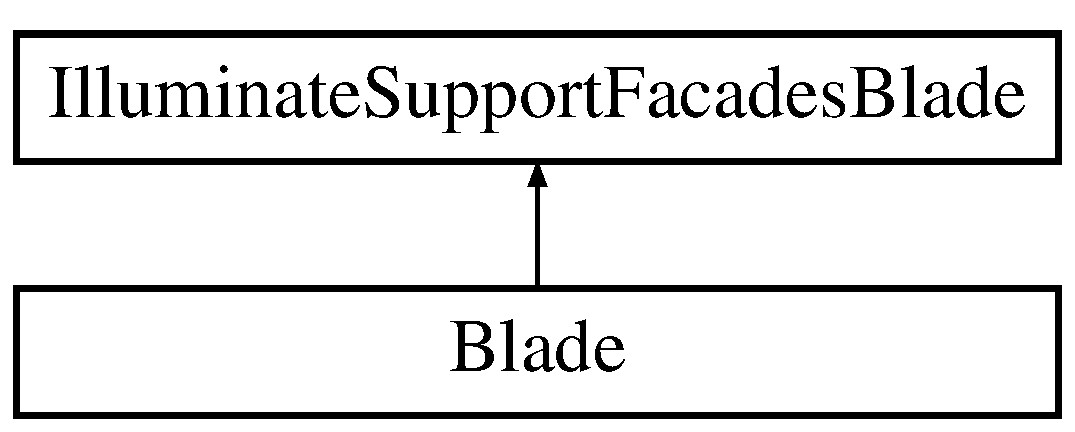
\includegraphics[height=2.000000cm]{class_illuminate_1_1_support_1_1_facades_1_1_blade}
\end{center}
\end{figure}
\subsection*{Static Public Member Functions}
\begin{DoxyCompactItemize}
\item 
static \mbox{\hyperlink{class_illuminate_1_1_support_1_1_facades_1_1_blade_a0a45f9e95e5f3d63a18ad1c57612e340}{compile}} (\$path=null)
\item 
static \mbox{\hyperlink{class_illuminate_1_1_support_1_1_facades_1_1_blade_af4cd0ba1505bbd09031711afe52adfca}{get\+Path}} ()
\item 
static \mbox{\hyperlink{class_illuminate_1_1_support_1_1_facades_1_1_blade_a09e64db7dab97caa40885f701d76057d}{set\+Path}} (\$path)
\item 
static \mbox{\hyperlink{class_illuminate_1_1_support_1_1_facades_1_1_blade_ace0d9e04307ea31f761025a62b3e3155}{compile\+String}} (\$value)
\item 
static \mbox{\hyperlink{class_illuminate_1_1_support_1_1_facades_1_1_blade_ac29fff878c323d136f3d9aa334adf9e6}{strip\+Parentheses}} (\$expression)
\item 
static \mbox{\hyperlink{class_illuminate_1_1_support_1_1_facades_1_1_blade_a69d90db30c898c05a0c4b4b0c951af05}{extend}} (\$compiler)
\item 
static \mbox{\hyperlink{class_illuminate_1_1_support_1_1_facades_1_1_blade_ac5cb8f56b82091732182cd9bd2b84280}{get\+Extensions}} ()
\item 
static \mbox{\hyperlink{class_illuminate_1_1_support_1_1_facades_1_1_blade_a268e95c7f7190f897af20e1819568fd9}{if}} (\$name, \$callback)
\item 
static \mbox{\hyperlink{class_illuminate_1_1_support_1_1_facades_1_1_blade_aebc299d130bd96397a458dba3b583d63}{check}} (\$name, \$parameters=null)
\item 
static \mbox{\hyperlink{class_illuminate_1_1_support_1_1_facades_1_1_blade_a52ae58875eaccfaac5d6bc3bf9ae5952}{directive}} (\$name, \$handler)
\item 
static \mbox{\hyperlink{class_illuminate_1_1_support_1_1_facades_1_1_blade_ae7d3ff8509253bb984d96981a2d89226}{get\+Custom\+Directives}} ()
\item 
static \mbox{\hyperlink{class_illuminate_1_1_support_1_1_facades_1_1_blade_abe61a53debc94f487f169ba8f98cc1b7}{set\+Echo\+Format}} (\$format)
\item 
static \mbox{\hyperlink{class_illuminate_1_1_support_1_1_facades_1_1_blade_a9b2f060067fc407f0c0bd893a141d74f}{get\+Compiled\+Path}} (\$path)
\item 
static \mbox{\hyperlink{class_illuminate_1_1_support_1_1_facades_1_1_blade_adea1a1e9be278d6c8bab02c5c097e819}{is\+Expired}} (\$path)
\item 
static \mbox{\hyperlink{class_illuminate_1_1_support_1_1_facades_1_1_blade_a97fb22faf14e93f58b47796b199955ea}{compile\+Echo\+Defaults}} (\$value)
\end{DoxyCompactItemize}


\subsection{Member Function Documentation}
\mbox{\Hypertarget{class_illuminate_1_1_support_1_1_facades_1_1_blade_aebc299d130bd96397a458dba3b583d63}\label{class_illuminate_1_1_support_1_1_facades_1_1_blade_aebc299d130bd96397a458dba3b583d63}} 
\index{Illuminate\+::\+Support\+::\+Facades\+::\+Blade@{Illuminate\+::\+Support\+::\+Facades\+::\+Blade}!check@{check}}
\index{check@{check}!Illuminate\+::\+Support\+::\+Facades\+::\+Blade@{Illuminate\+::\+Support\+::\+Facades\+::\+Blade}}
\subsubsection{\texorpdfstring{check()}{check()}}
{\footnotesize\ttfamily static Illuminate\textbackslash{}\+Support\textbackslash{}\+Facades\textbackslash{}\+Blade\+::check (\begin{DoxyParamCaption}\item[{}]{\$name,  }\item[{}]{\$parameters = {\ttfamily null} }\end{DoxyParamCaption})\hspace{0.3cm}{\ttfamily [static]}}

Check the result of a condition.


\begin{DoxyParams}[1]{Parameters}
string & {\em \$name} & \\
\hline
array & {\em \$parameters} & \\
\hline
\end{DoxyParams}
\begin{DoxyReturn}{Returns}
bool 
\end{DoxyReturn}
\mbox{\Hypertarget{class_illuminate_1_1_support_1_1_facades_1_1_blade_a0a45f9e95e5f3d63a18ad1c57612e340}\label{class_illuminate_1_1_support_1_1_facades_1_1_blade_a0a45f9e95e5f3d63a18ad1c57612e340}} 
\index{Illuminate\+::\+Support\+::\+Facades\+::\+Blade@{Illuminate\+::\+Support\+::\+Facades\+::\+Blade}!compile@{compile}}
\index{compile@{compile}!Illuminate\+::\+Support\+::\+Facades\+::\+Blade@{Illuminate\+::\+Support\+::\+Facades\+::\+Blade}}
\subsubsection{\texorpdfstring{compile()}{compile()}}
{\footnotesize\ttfamily static Illuminate\textbackslash{}\+Support\textbackslash{}\+Facades\textbackslash{}\+Blade\+::compile (\begin{DoxyParamCaption}\item[{}]{\$path = {\ttfamily null} }\end{DoxyParamCaption})\hspace{0.3cm}{\ttfamily [static]}}

Compile the view at the given path.


\begin{DoxyParams}[1]{Parameters}
string & {\em \$path} & \\
\hline
\end{DoxyParams}
\begin{DoxyReturn}{Returns}
void 
\end{DoxyReturn}
\mbox{\Hypertarget{class_illuminate_1_1_support_1_1_facades_1_1_blade_a97fb22faf14e93f58b47796b199955ea}\label{class_illuminate_1_1_support_1_1_facades_1_1_blade_a97fb22faf14e93f58b47796b199955ea}} 
\index{Illuminate\+::\+Support\+::\+Facades\+::\+Blade@{Illuminate\+::\+Support\+::\+Facades\+::\+Blade}!compile\+Echo\+Defaults@{compile\+Echo\+Defaults}}
\index{compile\+Echo\+Defaults@{compile\+Echo\+Defaults}!Illuminate\+::\+Support\+::\+Facades\+::\+Blade@{Illuminate\+::\+Support\+::\+Facades\+::\+Blade}}
\subsubsection{\texorpdfstring{compile\+Echo\+Defaults()}{compileEchoDefaults()}}
{\footnotesize\ttfamily static Illuminate\textbackslash{}\+Support\textbackslash{}\+Facades\textbackslash{}\+Blade\+::compile\+Echo\+Defaults (\begin{DoxyParamCaption}\item[{}]{\$value }\end{DoxyParamCaption})\hspace{0.3cm}{\ttfamily [static]}}

Compile the default values for the echo statement.


\begin{DoxyParams}[1]{Parameters}
string & {\em \$value} & \\
\hline
\end{DoxyParams}
\begin{DoxyReturn}{Returns}
string 
\end{DoxyReturn}
\mbox{\Hypertarget{class_illuminate_1_1_support_1_1_facades_1_1_blade_ace0d9e04307ea31f761025a62b3e3155}\label{class_illuminate_1_1_support_1_1_facades_1_1_blade_ace0d9e04307ea31f761025a62b3e3155}} 
\index{Illuminate\+::\+Support\+::\+Facades\+::\+Blade@{Illuminate\+::\+Support\+::\+Facades\+::\+Blade}!compile\+String@{compile\+String}}
\index{compile\+String@{compile\+String}!Illuminate\+::\+Support\+::\+Facades\+::\+Blade@{Illuminate\+::\+Support\+::\+Facades\+::\+Blade}}
\subsubsection{\texorpdfstring{compile\+String()}{compileString()}}
{\footnotesize\ttfamily static Illuminate\textbackslash{}\+Support\textbackslash{}\+Facades\textbackslash{}\+Blade\+::compile\+String (\begin{DoxyParamCaption}\item[{}]{\$value }\end{DoxyParamCaption})\hspace{0.3cm}{\ttfamily [static]}}

Compile the given \mbox{\hyperlink{class_illuminate_1_1_support_1_1_facades_1_1_blade}{Blade}} template contents.


\begin{DoxyParams}[1]{Parameters}
string & {\em \$value} & \\
\hline
\end{DoxyParams}
\begin{DoxyReturn}{Returns}
string 
\end{DoxyReturn}
\mbox{\Hypertarget{class_illuminate_1_1_support_1_1_facades_1_1_blade_a52ae58875eaccfaac5d6bc3bf9ae5952}\label{class_illuminate_1_1_support_1_1_facades_1_1_blade_a52ae58875eaccfaac5d6bc3bf9ae5952}} 
\index{Illuminate\+::\+Support\+::\+Facades\+::\+Blade@{Illuminate\+::\+Support\+::\+Facades\+::\+Blade}!directive@{directive}}
\index{directive@{directive}!Illuminate\+::\+Support\+::\+Facades\+::\+Blade@{Illuminate\+::\+Support\+::\+Facades\+::\+Blade}}
\subsubsection{\texorpdfstring{directive()}{directive()}}
{\footnotesize\ttfamily static Illuminate\textbackslash{}\+Support\textbackslash{}\+Facades\textbackslash{}\+Blade\+::directive (\begin{DoxyParamCaption}\item[{}]{\$name,  }\item[{}]{\$handler }\end{DoxyParamCaption})\hspace{0.3cm}{\ttfamily [static]}}

Register a handler for custom directives.


\begin{DoxyParams}[1]{Parameters}
string & {\em \$name} & \\
\hline
callable & {\em \$handler} & \\
\hline
\end{DoxyParams}
\begin{DoxyReturn}{Returns}
void 
\end{DoxyReturn}
\mbox{\Hypertarget{class_illuminate_1_1_support_1_1_facades_1_1_blade_a69d90db30c898c05a0c4b4b0c951af05}\label{class_illuminate_1_1_support_1_1_facades_1_1_blade_a69d90db30c898c05a0c4b4b0c951af05}} 
\index{Illuminate\+::\+Support\+::\+Facades\+::\+Blade@{Illuminate\+::\+Support\+::\+Facades\+::\+Blade}!extend@{extend}}
\index{extend@{extend}!Illuminate\+::\+Support\+::\+Facades\+::\+Blade@{Illuminate\+::\+Support\+::\+Facades\+::\+Blade}}
\subsubsection{\texorpdfstring{extend()}{extend()}}
{\footnotesize\ttfamily static Illuminate\textbackslash{}\+Support\textbackslash{}\+Facades\textbackslash{}\+Blade\+::extend (\begin{DoxyParamCaption}\item[{}]{\$compiler }\end{DoxyParamCaption})\hspace{0.3cm}{\ttfamily [static]}}

Register a custom \mbox{\hyperlink{class_illuminate_1_1_support_1_1_facades_1_1_blade}{Blade}} compiler.


\begin{DoxyParams}[1]{Parameters}
callable & {\em \$compiler} & \\
\hline
\end{DoxyParams}
\begin{DoxyReturn}{Returns}
void 
\end{DoxyReturn}
\mbox{\Hypertarget{class_illuminate_1_1_support_1_1_facades_1_1_blade_a9b2f060067fc407f0c0bd893a141d74f}\label{class_illuminate_1_1_support_1_1_facades_1_1_blade_a9b2f060067fc407f0c0bd893a141d74f}} 
\index{Illuminate\+::\+Support\+::\+Facades\+::\+Blade@{Illuminate\+::\+Support\+::\+Facades\+::\+Blade}!get\+Compiled\+Path@{get\+Compiled\+Path}}
\index{get\+Compiled\+Path@{get\+Compiled\+Path}!Illuminate\+::\+Support\+::\+Facades\+::\+Blade@{Illuminate\+::\+Support\+::\+Facades\+::\+Blade}}
\subsubsection{\texorpdfstring{get\+Compiled\+Path()}{getCompiledPath()}}
{\footnotesize\ttfamily static Illuminate\textbackslash{}\+Support\textbackslash{}\+Facades\textbackslash{}\+Blade\+::get\+Compiled\+Path (\begin{DoxyParamCaption}\item[{}]{\$path }\end{DoxyParamCaption})\hspace{0.3cm}{\ttfamily [static]}}

Get the path to the compiled version of a view.


\begin{DoxyParams}[1]{Parameters}
string & {\em \$path} & \\
\hline
\end{DoxyParams}
\begin{DoxyReturn}{Returns}
string 
\end{DoxyReturn}
\mbox{\Hypertarget{class_illuminate_1_1_support_1_1_facades_1_1_blade_ae7d3ff8509253bb984d96981a2d89226}\label{class_illuminate_1_1_support_1_1_facades_1_1_blade_ae7d3ff8509253bb984d96981a2d89226}} 
\index{Illuminate\+::\+Support\+::\+Facades\+::\+Blade@{Illuminate\+::\+Support\+::\+Facades\+::\+Blade}!get\+Custom\+Directives@{get\+Custom\+Directives}}
\index{get\+Custom\+Directives@{get\+Custom\+Directives}!Illuminate\+::\+Support\+::\+Facades\+::\+Blade@{Illuminate\+::\+Support\+::\+Facades\+::\+Blade}}
\subsubsection{\texorpdfstring{get\+Custom\+Directives()}{getCustomDirectives()}}
{\footnotesize\ttfamily static Illuminate\textbackslash{}\+Support\textbackslash{}\+Facades\textbackslash{}\+Blade\+::get\+Custom\+Directives (\begin{DoxyParamCaption}{ }\end{DoxyParamCaption})\hspace{0.3cm}{\ttfamily [static]}}

Get the list of custom directives.

\begin{DoxyReturn}{Returns}
array 
\end{DoxyReturn}
\mbox{\Hypertarget{class_illuminate_1_1_support_1_1_facades_1_1_blade_ac5cb8f56b82091732182cd9bd2b84280}\label{class_illuminate_1_1_support_1_1_facades_1_1_blade_ac5cb8f56b82091732182cd9bd2b84280}} 
\index{Illuminate\+::\+Support\+::\+Facades\+::\+Blade@{Illuminate\+::\+Support\+::\+Facades\+::\+Blade}!get\+Extensions@{get\+Extensions}}
\index{get\+Extensions@{get\+Extensions}!Illuminate\+::\+Support\+::\+Facades\+::\+Blade@{Illuminate\+::\+Support\+::\+Facades\+::\+Blade}}
\subsubsection{\texorpdfstring{get\+Extensions()}{getExtensions()}}
{\footnotesize\ttfamily static Illuminate\textbackslash{}\+Support\textbackslash{}\+Facades\textbackslash{}\+Blade\+::get\+Extensions (\begin{DoxyParamCaption}{ }\end{DoxyParamCaption})\hspace{0.3cm}{\ttfamily [static]}}

Get the extensions used by the compiler.

\begin{DoxyReturn}{Returns}
array 
\end{DoxyReturn}
\mbox{\Hypertarget{class_illuminate_1_1_support_1_1_facades_1_1_blade_af4cd0ba1505bbd09031711afe52adfca}\label{class_illuminate_1_1_support_1_1_facades_1_1_blade_af4cd0ba1505bbd09031711afe52adfca}} 
\index{Illuminate\+::\+Support\+::\+Facades\+::\+Blade@{Illuminate\+::\+Support\+::\+Facades\+::\+Blade}!get\+Path@{get\+Path}}
\index{get\+Path@{get\+Path}!Illuminate\+::\+Support\+::\+Facades\+::\+Blade@{Illuminate\+::\+Support\+::\+Facades\+::\+Blade}}
\subsubsection{\texorpdfstring{get\+Path()}{getPath()}}
{\footnotesize\ttfamily static Illuminate\textbackslash{}\+Support\textbackslash{}\+Facades\textbackslash{}\+Blade\+::get\+Path (\begin{DoxyParamCaption}{ }\end{DoxyParamCaption})\hspace{0.3cm}{\ttfamily [static]}}

Get the path currently being compiled.

\begin{DoxyReturn}{Returns}
string 
\end{DoxyReturn}
\mbox{\Hypertarget{class_illuminate_1_1_support_1_1_facades_1_1_blade_a268e95c7f7190f897af20e1819568fd9}\label{class_illuminate_1_1_support_1_1_facades_1_1_blade_a268e95c7f7190f897af20e1819568fd9}} 
\index{Illuminate\+::\+Support\+::\+Facades\+::\+Blade@{Illuminate\+::\+Support\+::\+Facades\+::\+Blade}!if@{if}}
\index{if@{if}!Illuminate\+::\+Support\+::\+Facades\+::\+Blade@{Illuminate\+::\+Support\+::\+Facades\+::\+Blade}}
\subsubsection{\texorpdfstring{if()}{if()}}
{\footnotesize\ttfamily static Illuminate\textbackslash{}\+Support\textbackslash{}\+Facades\textbackslash{}\+Blade\+::if (\begin{DoxyParamCaption}\item[{}]{\$name,  }\item[{}]{\$callback }\end{DoxyParamCaption})\hspace{0.3cm}{\ttfamily [static]}}

Register an \char`\"{}if\char`\"{} statement directive.


\begin{DoxyParams}[1]{Parameters}
string & {\em \$name} & \\
\hline
callable & {\em \$callback} & \\
\hline
\end{DoxyParams}
\begin{DoxyReturn}{Returns}
void 
\end{DoxyReturn}
\mbox{\Hypertarget{class_illuminate_1_1_support_1_1_facades_1_1_blade_adea1a1e9be278d6c8bab02c5c097e819}\label{class_illuminate_1_1_support_1_1_facades_1_1_blade_adea1a1e9be278d6c8bab02c5c097e819}} 
\index{Illuminate\+::\+Support\+::\+Facades\+::\+Blade@{Illuminate\+::\+Support\+::\+Facades\+::\+Blade}!is\+Expired@{is\+Expired}}
\index{is\+Expired@{is\+Expired}!Illuminate\+::\+Support\+::\+Facades\+::\+Blade@{Illuminate\+::\+Support\+::\+Facades\+::\+Blade}}
\subsubsection{\texorpdfstring{is\+Expired()}{isExpired()}}
{\footnotesize\ttfamily static Illuminate\textbackslash{}\+Support\textbackslash{}\+Facades\textbackslash{}\+Blade\+::is\+Expired (\begin{DoxyParamCaption}\item[{}]{\$path }\end{DoxyParamCaption})\hspace{0.3cm}{\ttfamily [static]}}

Determine if the view at the given path is expired.


\begin{DoxyParams}[1]{Parameters}
string & {\em \$path} & \\
\hline
\end{DoxyParams}
\begin{DoxyReturn}{Returns}
bool 
\end{DoxyReturn}
\mbox{\Hypertarget{class_illuminate_1_1_support_1_1_facades_1_1_blade_abe61a53debc94f487f169ba8f98cc1b7}\label{class_illuminate_1_1_support_1_1_facades_1_1_blade_abe61a53debc94f487f169ba8f98cc1b7}} 
\index{Illuminate\+::\+Support\+::\+Facades\+::\+Blade@{Illuminate\+::\+Support\+::\+Facades\+::\+Blade}!set\+Echo\+Format@{set\+Echo\+Format}}
\index{set\+Echo\+Format@{set\+Echo\+Format}!Illuminate\+::\+Support\+::\+Facades\+::\+Blade@{Illuminate\+::\+Support\+::\+Facades\+::\+Blade}}
\subsubsection{\texorpdfstring{set\+Echo\+Format()}{setEchoFormat()}}
{\footnotesize\ttfamily static Illuminate\textbackslash{}\+Support\textbackslash{}\+Facades\textbackslash{}\+Blade\+::set\+Echo\+Format (\begin{DoxyParamCaption}\item[{}]{\$format }\end{DoxyParamCaption})\hspace{0.3cm}{\ttfamily [static]}}

Set the echo format to be used by the compiler.


\begin{DoxyParams}[1]{Parameters}
string & {\em \$format} & \\
\hline
\end{DoxyParams}
\begin{DoxyReturn}{Returns}
void 
\end{DoxyReturn}
\mbox{\Hypertarget{class_illuminate_1_1_support_1_1_facades_1_1_blade_a09e64db7dab97caa40885f701d76057d}\label{class_illuminate_1_1_support_1_1_facades_1_1_blade_a09e64db7dab97caa40885f701d76057d}} 
\index{Illuminate\+::\+Support\+::\+Facades\+::\+Blade@{Illuminate\+::\+Support\+::\+Facades\+::\+Blade}!set\+Path@{set\+Path}}
\index{set\+Path@{set\+Path}!Illuminate\+::\+Support\+::\+Facades\+::\+Blade@{Illuminate\+::\+Support\+::\+Facades\+::\+Blade}}
\subsubsection{\texorpdfstring{set\+Path()}{setPath()}}
{\footnotesize\ttfamily static Illuminate\textbackslash{}\+Support\textbackslash{}\+Facades\textbackslash{}\+Blade\+::set\+Path (\begin{DoxyParamCaption}\item[{}]{\$path }\end{DoxyParamCaption})\hspace{0.3cm}{\ttfamily [static]}}

Set the path currently being compiled.


\begin{DoxyParams}[1]{Parameters}
string & {\em \$path} & \\
\hline
\end{DoxyParams}
\begin{DoxyReturn}{Returns}
void 
\end{DoxyReturn}
\mbox{\Hypertarget{class_illuminate_1_1_support_1_1_facades_1_1_blade_ac29fff878c323d136f3d9aa334adf9e6}\label{class_illuminate_1_1_support_1_1_facades_1_1_blade_ac29fff878c323d136f3d9aa334adf9e6}} 
\index{Illuminate\+::\+Support\+::\+Facades\+::\+Blade@{Illuminate\+::\+Support\+::\+Facades\+::\+Blade}!strip\+Parentheses@{strip\+Parentheses}}
\index{strip\+Parentheses@{strip\+Parentheses}!Illuminate\+::\+Support\+::\+Facades\+::\+Blade@{Illuminate\+::\+Support\+::\+Facades\+::\+Blade}}
\subsubsection{\texorpdfstring{strip\+Parentheses()}{stripParentheses()}}
{\footnotesize\ttfamily static Illuminate\textbackslash{}\+Support\textbackslash{}\+Facades\textbackslash{}\+Blade\+::strip\+Parentheses (\begin{DoxyParamCaption}\item[{}]{\$expression }\end{DoxyParamCaption})\hspace{0.3cm}{\ttfamily [static]}}

Strip the parentheses from the given expression.


\begin{DoxyParams}[1]{Parameters}
string & {\em \$expression} & \\
\hline
\end{DoxyParams}
\begin{DoxyReturn}{Returns}
string 
\end{DoxyReturn}


The documentation for this class was generated from the following file\+:\begin{DoxyCompactItemize}
\item 
\+\_\+ide\+\_\+helper.\+php\end{DoxyCompactItemize}

\hypertarget{class_blade}{}\section{Blade Class Reference}
\label{class_blade}\index{Blade@{Blade}}
Inheritance diagram for Blade\+:\begin{figure}[H]
\begin{center}
\leavevmode
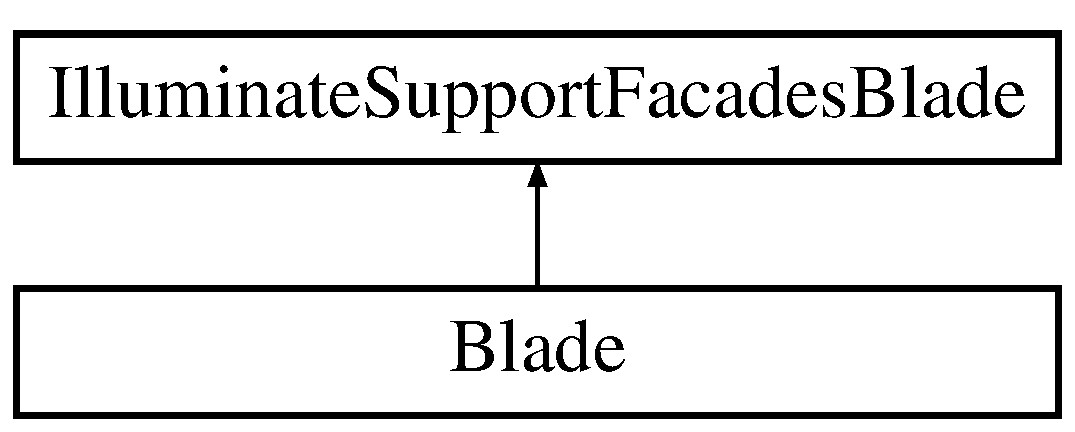
\includegraphics[height=2.000000cm]{class_blade}
\end{center}
\end{figure}
\subsection*{Additional Inherited Members}


The documentation for this class was generated from the following file\+:\begin{DoxyCompactItemize}
\item 
\+\_\+ide\+\_\+helper.\+php\end{DoxyCompactItemize}

\hypertarget{class_broadcast}{}\section{Broadcast Class Reference}
\label{class_broadcast}\index{Broadcast@{Broadcast}}
Inheritance diagram for Broadcast\+:\begin{figure}[H]
\begin{center}
\leavevmode
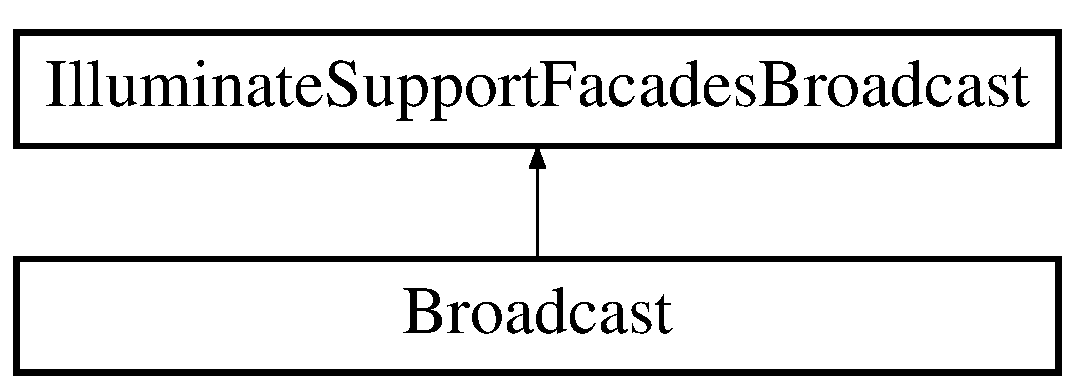
\includegraphics[height=2.000000cm]{class_broadcast}
\end{center}
\end{figure}
\subsection*{Additional Inherited Members}


The documentation for this class was generated from the following file\+:\begin{DoxyCompactItemize}
\item 
\+\_\+ide\+\_\+helper.\+php\end{DoxyCompactItemize}

\hypertarget{class_illuminate_1_1_support_1_1_facades_1_1_broadcast}{}\section{Illuminate\textbackslash{}Support\textbackslash{}Facades\textbackslash{}Broadcast Class Reference}
\label{class_illuminate_1_1_support_1_1_facades_1_1_broadcast}\index{Illuminate\textbackslash{}\+Support\textbackslash{}\+Facades\textbackslash{}\+Broadcast@{Illuminate\textbackslash{}\+Support\textbackslash{}\+Facades\textbackslash{}\+Broadcast}}
Inheritance diagram for Illuminate\textbackslash{}Support\textbackslash{}Facades\textbackslash{}Broadcast\+:\begin{figure}[H]
\begin{center}
\leavevmode
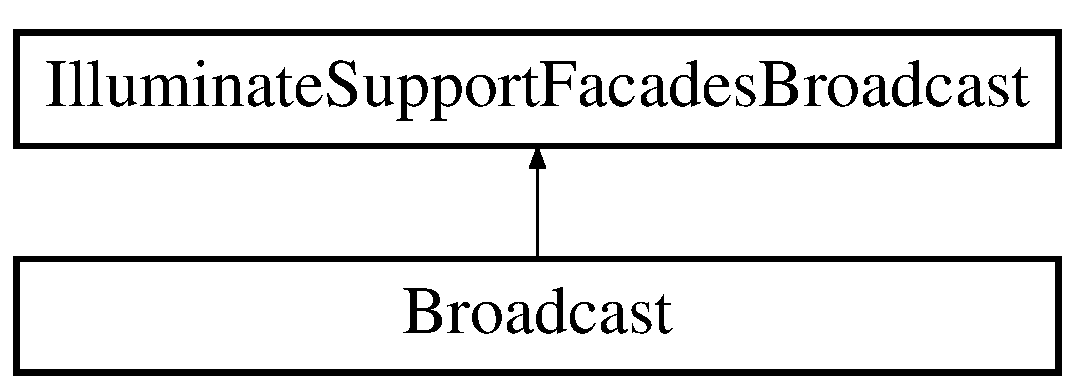
\includegraphics[height=2.000000cm]{class_illuminate_1_1_support_1_1_facades_1_1_broadcast}
\end{center}
\end{figure}
\subsection*{Static Public Member Functions}
\begin{DoxyCompactItemize}
\item 
static \mbox{\hyperlink{class_illuminate_1_1_support_1_1_facades_1_1_broadcast_a7b01f8f6feddd98350be0def6f2ec6fd}{routes}} (\$attributes=null)
\item 
static \mbox{\hyperlink{class_illuminate_1_1_support_1_1_facades_1_1_broadcast_a6a4b121169824b3e5153107ad3d98044}{socket}} (\$request=null)
\item 
static \mbox{\hyperlink{class_illuminate_1_1_support_1_1_facades_1_1_broadcast_af0187828ad8e637972903b98eb345b70}{event}} (\$event=null)
\item 
static \mbox{\hyperlink{class_illuminate_1_1_support_1_1_facades_1_1_broadcast_a25f11be8ae7dd784f6b7f0930fcb8ef1}{queue}} (\$\mbox{\hyperlink{class_illuminate_1_1_support_1_1_facades_1_1_broadcast_af0187828ad8e637972903b98eb345b70}{event}})
\item 
static \mbox{\hyperlink{class_illuminate_1_1_support_1_1_facades_1_1_broadcast_ab5a3d97c5bad4cb46537b4396e93bc2b}{connection}} (\$\mbox{\hyperlink{class_illuminate_1_1_support_1_1_facades_1_1_broadcast_a9bdbd5d1fd001e1a5ef02b4003f8d552}{driver}}=null)
\item 
static \mbox{\hyperlink{class_illuminate_1_1_support_1_1_facades_1_1_broadcast_a9bdbd5d1fd001e1a5ef02b4003f8d552}{driver}} (\$name=null)
\item 
static \mbox{\hyperlink{class_illuminate_1_1_support_1_1_facades_1_1_broadcast_a38fa0a82b75503dddc1675b02644ba10}{get\+Default\+Driver}} ()
\item 
static \mbox{\hyperlink{class_illuminate_1_1_support_1_1_facades_1_1_broadcast_ae7f1533413aa1c6235a5d581f042656f}{set\+Default\+Driver}} (\$name)
\item 
static \mbox{\hyperlink{class_illuminate_1_1_support_1_1_facades_1_1_broadcast_a644492e0fbd34d13c70db1692e1d01b0}{extend}} (\$\mbox{\hyperlink{class_illuminate_1_1_support_1_1_facades_1_1_broadcast_a9bdbd5d1fd001e1a5ef02b4003f8d552}{driver}}, \$callback)
\end{DoxyCompactItemize}


\subsection{Member Function Documentation}
\mbox{\Hypertarget{class_illuminate_1_1_support_1_1_facades_1_1_broadcast_ab5a3d97c5bad4cb46537b4396e93bc2b}\label{class_illuminate_1_1_support_1_1_facades_1_1_broadcast_ab5a3d97c5bad4cb46537b4396e93bc2b}} 
\index{Illuminate\+::\+Support\+::\+Facades\+::\+Broadcast@{Illuminate\+::\+Support\+::\+Facades\+::\+Broadcast}!connection@{connection}}
\index{connection@{connection}!Illuminate\+::\+Support\+::\+Facades\+::\+Broadcast@{Illuminate\+::\+Support\+::\+Facades\+::\+Broadcast}}
\subsubsection{\texorpdfstring{connection()}{connection()}}
{\footnotesize\ttfamily static Illuminate\textbackslash{}\+Support\textbackslash{}\+Facades\textbackslash{}\+Broadcast\+::connection (\begin{DoxyParamCaption}\item[{}]{\$driver = {\ttfamily null} }\end{DoxyParamCaption})\hspace{0.3cm}{\ttfamily [static]}}

Get a driver instance.


\begin{DoxyParams}[1]{Parameters}
string & {\em \$driver} & \\
\hline
\end{DoxyParams}
\begin{DoxyReturn}{Returns}
mixed 
\end{DoxyReturn}
\mbox{\Hypertarget{class_illuminate_1_1_support_1_1_facades_1_1_broadcast_a9bdbd5d1fd001e1a5ef02b4003f8d552}\label{class_illuminate_1_1_support_1_1_facades_1_1_broadcast_a9bdbd5d1fd001e1a5ef02b4003f8d552}} 
\index{Illuminate\+::\+Support\+::\+Facades\+::\+Broadcast@{Illuminate\+::\+Support\+::\+Facades\+::\+Broadcast}!driver@{driver}}
\index{driver@{driver}!Illuminate\+::\+Support\+::\+Facades\+::\+Broadcast@{Illuminate\+::\+Support\+::\+Facades\+::\+Broadcast}}
\subsubsection{\texorpdfstring{driver()}{driver()}}
{\footnotesize\ttfamily static Illuminate\textbackslash{}\+Support\textbackslash{}\+Facades\textbackslash{}\+Broadcast\+::driver (\begin{DoxyParamCaption}\item[{}]{\$name = {\ttfamily null} }\end{DoxyParamCaption})\hspace{0.3cm}{\ttfamily [static]}}

Get a driver instance.


\begin{DoxyParams}[1]{Parameters}
string & {\em \$name} & \\
\hline
\end{DoxyParams}
\begin{DoxyReturn}{Returns}
mixed 
\end{DoxyReturn}
\mbox{\Hypertarget{class_illuminate_1_1_support_1_1_facades_1_1_broadcast_af0187828ad8e637972903b98eb345b70}\label{class_illuminate_1_1_support_1_1_facades_1_1_broadcast_af0187828ad8e637972903b98eb345b70}} 
\index{Illuminate\+::\+Support\+::\+Facades\+::\+Broadcast@{Illuminate\+::\+Support\+::\+Facades\+::\+Broadcast}!event@{event}}
\index{event@{event}!Illuminate\+::\+Support\+::\+Facades\+::\+Broadcast@{Illuminate\+::\+Support\+::\+Facades\+::\+Broadcast}}
\subsubsection{\texorpdfstring{event()}{event()}}
{\footnotesize\ttfamily static Illuminate\textbackslash{}\+Support\textbackslash{}\+Facades\textbackslash{}\+Broadcast\+::event (\begin{DoxyParamCaption}\item[{}]{\$event = {\ttfamily null} }\end{DoxyParamCaption})\hspace{0.3cm}{\ttfamily [static]}}

Begin broadcasting an event.


\begin{DoxyParams}[1]{Parameters}
mixed | null & {\em \$event} & \\
\hline
\end{DoxyParams}
\begin{DoxyReturn}{Returns}
$\vert$void 
\end{DoxyReturn}
\mbox{\Hypertarget{class_illuminate_1_1_support_1_1_facades_1_1_broadcast_a644492e0fbd34d13c70db1692e1d01b0}\label{class_illuminate_1_1_support_1_1_facades_1_1_broadcast_a644492e0fbd34d13c70db1692e1d01b0}} 
\index{Illuminate\+::\+Support\+::\+Facades\+::\+Broadcast@{Illuminate\+::\+Support\+::\+Facades\+::\+Broadcast}!extend@{extend}}
\index{extend@{extend}!Illuminate\+::\+Support\+::\+Facades\+::\+Broadcast@{Illuminate\+::\+Support\+::\+Facades\+::\+Broadcast}}
\subsubsection{\texorpdfstring{extend()}{extend()}}
{\footnotesize\ttfamily static Illuminate\textbackslash{}\+Support\textbackslash{}\+Facades\textbackslash{}\+Broadcast\+::extend (\begin{DoxyParamCaption}\item[{}]{\$driver,  }\item[{}]{\$callback }\end{DoxyParamCaption})\hspace{0.3cm}{\ttfamily [static]}}

Register a custom driver creator Closure.


\begin{DoxyParams}[1]{Parameters}
string & {\em \$driver} & \\
\hline
\textbackslash{}\+Closure & {\em \$callback} & \\
\hline
\end{DoxyParams}
\begin{DoxyReturn}{Returns}
\$this 
\end{DoxyReturn}
\mbox{\Hypertarget{class_illuminate_1_1_support_1_1_facades_1_1_broadcast_a38fa0a82b75503dddc1675b02644ba10}\label{class_illuminate_1_1_support_1_1_facades_1_1_broadcast_a38fa0a82b75503dddc1675b02644ba10}} 
\index{Illuminate\+::\+Support\+::\+Facades\+::\+Broadcast@{Illuminate\+::\+Support\+::\+Facades\+::\+Broadcast}!get\+Default\+Driver@{get\+Default\+Driver}}
\index{get\+Default\+Driver@{get\+Default\+Driver}!Illuminate\+::\+Support\+::\+Facades\+::\+Broadcast@{Illuminate\+::\+Support\+::\+Facades\+::\+Broadcast}}
\subsubsection{\texorpdfstring{get\+Default\+Driver()}{getDefaultDriver()}}
{\footnotesize\ttfamily static Illuminate\textbackslash{}\+Support\textbackslash{}\+Facades\textbackslash{}\+Broadcast\+::get\+Default\+Driver (\begin{DoxyParamCaption}{ }\end{DoxyParamCaption})\hspace{0.3cm}{\ttfamily [static]}}

Get the default driver name.

\begin{DoxyReturn}{Returns}
string 
\end{DoxyReturn}
\mbox{\Hypertarget{class_illuminate_1_1_support_1_1_facades_1_1_broadcast_a25f11be8ae7dd784f6b7f0930fcb8ef1}\label{class_illuminate_1_1_support_1_1_facades_1_1_broadcast_a25f11be8ae7dd784f6b7f0930fcb8ef1}} 
\index{Illuminate\+::\+Support\+::\+Facades\+::\+Broadcast@{Illuminate\+::\+Support\+::\+Facades\+::\+Broadcast}!queue@{queue}}
\index{queue@{queue}!Illuminate\+::\+Support\+::\+Facades\+::\+Broadcast@{Illuminate\+::\+Support\+::\+Facades\+::\+Broadcast}}
\subsubsection{\texorpdfstring{queue()}{queue()}}
{\footnotesize\ttfamily static Illuminate\textbackslash{}\+Support\textbackslash{}\+Facades\textbackslash{}\+Broadcast\+::queue (\begin{DoxyParamCaption}\item[{}]{\$event }\end{DoxyParamCaption})\hspace{0.3cm}{\ttfamily [static]}}

\mbox{\hyperlink{class_illuminate_1_1_support_1_1_facades_1_1_queue}{Queue}} the given event for broadcast.


\begin{DoxyParams}[1]{Parameters}
mixed & {\em \$event} & \\
\hline
\end{DoxyParams}
\begin{DoxyReturn}{Returns}
void 
\end{DoxyReturn}
\mbox{\Hypertarget{class_illuminate_1_1_support_1_1_facades_1_1_broadcast_a7b01f8f6feddd98350be0def6f2ec6fd}\label{class_illuminate_1_1_support_1_1_facades_1_1_broadcast_a7b01f8f6feddd98350be0def6f2ec6fd}} 
\index{Illuminate\+::\+Support\+::\+Facades\+::\+Broadcast@{Illuminate\+::\+Support\+::\+Facades\+::\+Broadcast}!routes@{routes}}
\index{routes@{routes}!Illuminate\+::\+Support\+::\+Facades\+::\+Broadcast@{Illuminate\+::\+Support\+::\+Facades\+::\+Broadcast}}
\subsubsection{\texorpdfstring{routes()}{routes()}}
{\footnotesize\ttfamily static Illuminate\textbackslash{}\+Support\textbackslash{}\+Facades\textbackslash{}\+Broadcast\+::routes (\begin{DoxyParamCaption}\item[{}]{\$attributes = {\ttfamily null} }\end{DoxyParamCaption})\hspace{0.3cm}{\ttfamily [static]}}

Register the routes for handling broadcast authentication and sockets.


\begin{DoxyParams}[1]{Parameters}
array | null & {\em \$attributes} & \\
\hline
\end{DoxyParams}
\begin{DoxyReturn}{Returns}
void 
\end{DoxyReturn}
\mbox{\Hypertarget{class_illuminate_1_1_support_1_1_facades_1_1_broadcast_ae7f1533413aa1c6235a5d581f042656f}\label{class_illuminate_1_1_support_1_1_facades_1_1_broadcast_ae7f1533413aa1c6235a5d581f042656f}} 
\index{Illuminate\+::\+Support\+::\+Facades\+::\+Broadcast@{Illuminate\+::\+Support\+::\+Facades\+::\+Broadcast}!set\+Default\+Driver@{set\+Default\+Driver}}
\index{set\+Default\+Driver@{set\+Default\+Driver}!Illuminate\+::\+Support\+::\+Facades\+::\+Broadcast@{Illuminate\+::\+Support\+::\+Facades\+::\+Broadcast}}
\subsubsection{\texorpdfstring{set\+Default\+Driver()}{setDefaultDriver()}}
{\footnotesize\ttfamily static Illuminate\textbackslash{}\+Support\textbackslash{}\+Facades\textbackslash{}\+Broadcast\+::set\+Default\+Driver (\begin{DoxyParamCaption}\item[{}]{\$name }\end{DoxyParamCaption})\hspace{0.3cm}{\ttfamily [static]}}

Set the default driver name.


\begin{DoxyParams}[1]{Parameters}
string & {\em \$name} & \\
\hline
\end{DoxyParams}
\begin{DoxyReturn}{Returns}
void 
\end{DoxyReturn}
\mbox{\Hypertarget{class_illuminate_1_1_support_1_1_facades_1_1_broadcast_a6a4b121169824b3e5153107ad3d98044}\label{class_illuminate_1_1_support_1_1_facades_1_1_broadcast_a6a4b121169824b3e5153107ad3d98044}} 
\index{Illuminate\+::\+Support\+::\+Facades\+::\+Broadcast@{Illuminate\+::\+Support\+::\+Facades\+::\+Broadcast}!socket@{socket}}
\index{socket@{socket}!Illuminate\+::\+Support\+::\+Facades\+::\+Broadcast@{Illuminate\+::\+Support\+::\+Facades\+::\+Broadcast}}
\subsubsection{\texorpdfstring{socket()}{socket()}}
{\footnotesize\ttfamily static Illuminate\textbackslash{}\+Support\textbackslash{}\+Facades\textbackslash{}\+Broadcast\+::socket (\begin{DoxyParamCaption}\item[{}]{\$request = {\ttfamily null} }\end{DoxyParamCaption})\hspace{0.3cm}{\ttfamily [static]}}

Get the socket ID for the given request.


\begin{DoxyParams}[1]{Parameters}
\textbackslash{}\+Illuminate\textbackslash{}\+Http\textbackslash{}\+Request | null & {\em \$request} & \\
\hline
\end{DoxyParams}
\begin{DoxyReturn}{Returns}
string$\vert$null 
\end{DoxyReturn}


The documentation for this class was generated from the following file\+:\begin{DoxyCompactItemize}
\item 
\+\_\+ide\+\_\+helper.\+php\end{DoxyCompactItemize}

\hypertarget{class_bus}{}\section{Bus Class Reference}
\label{class_bus}\index{Bus@{Bus}}
Inheritance diagram for Bus\+:\begin{figure}[H]
\begin{center}
\leavevmode
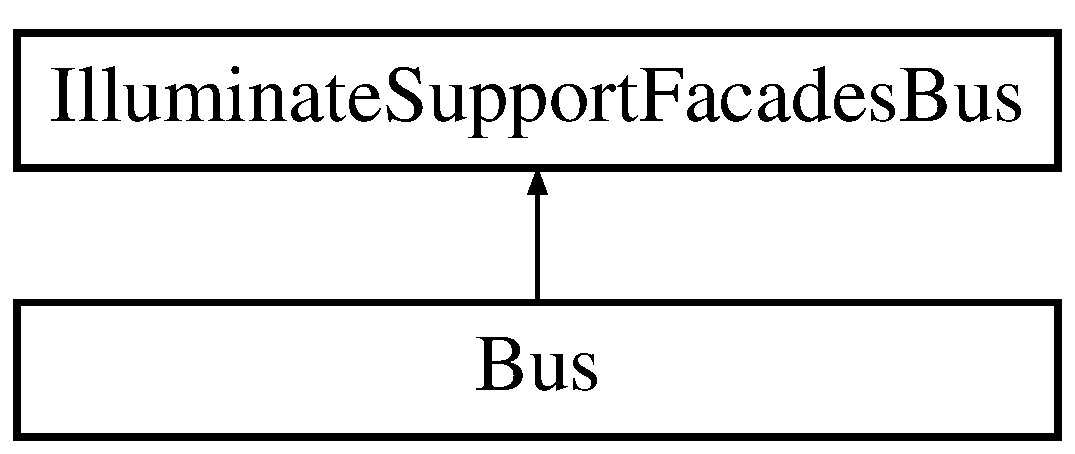
\includegraphics[height=2.000000cm]{class_bus}
\end{center}
\end{figure}
\subsection*{Additional Inherited Members}


The documentation for this class was generated from the following file\+:\begin{DoxyCompactItemize}
\item 
\+\_\+ide\+\_\+helper.\+php\end{DoxyCompactItemize}

\hypertarget{class_illuminate_1_1_support_1_1_facades_1_1_bus}{}\section{Illuminate\textbackslash{}Support\textbackslash{}Facades\textbackslash{}Bus Class Reference}
\label{class_illuminate_1_1_support_1_1_facades_1_1_bus}\index{Illuminate\textbackslash{}\+Support\textbackslash{}\+Facades\textbackslash{}\+Bus@{Illuminate\textbackslash{}\+Support\textbackslash{}\+Facades\textbackslash{}\+Bus}}
Inheritance diagram for Illuminate\textbackslash{}Support\textbackslash{}Facades\textbackslash{}Bus\+:\begin{figure}[H]
\begin{center}
\leavevmode
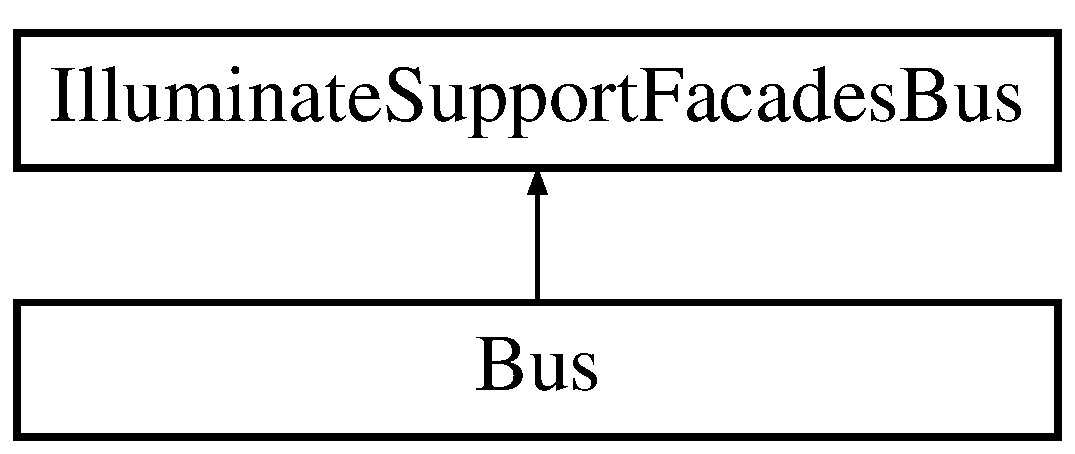
\includegraphics[height=2.000000cm]{class_illuminate_1_1_support_1_1_facades_1_1_bus}
\end{center}
\end{figure}
\subsection*{Static Public Member Functions}
\begin{DoxyCompactItemize}
\item 
static \mbox{\hyperlink{class_illuminate_1_1_support_1_1_facades_1_1_bus_af590935cb141b08cecb4a2e3222f9ce9}{dispatch}} (\$command)
\item 
static \mbox{\hyperlink{class_illuminate_1_1_support_1_1_facades_1_1_bus_a235f374bf88ac804ee020ae351f3ed0e}{dispatch\+Now}} (\$command, \$handler=null)
\item 
static \mbox{\hyperlink{class_illuminate_1_1_support_1_1_facades_1_1_bus_a9ce6c02e0ce39585a360f85c34c4bc42}{has\+Command\+Handler}} (\$command)
\item 
static \mbox{\hyperlink{class_illuminate_1_1_support_1_1_facades_1_1_bus_a4022c67963c0e29af464d885698d2c66}{get\+Command\+Handler}} (\$command)
\item 
static \mbox{\hyperlink{class_illuminate_1_1_support_1_1_facades_1_1_bus_a3975eb2e49eabbe74a6c784eb076c925}{dispatch\+To\+Queue}} (\$command)
\item 
static \mbox{\hyperlink{class_illuminate_1_1_support_1_1_facades_1_1_bus_ad04e2fde658dcbb3e583365f665c7381}{pipe\+Through}} (\$pipes)
\item 
static \mbox{\hyperlink{class_illuminate_1_1_support_1_1_facades_1_1_bus_a944bb1fc82a5d13749d20d31b1da9a9a}{map}} (\$map)
\end{DoxyCompactItemize}


\subsection{Member Function Documentation}
\mbox{\Hypertarget{class_illuminate_1_1_support_1_1_facades_1_1_bus_af590935cb141b08cecb4a2e3222f9ce9}\label{class_illuminate_1_1_support_1_1_facades_1_1_bus_af590935cb141b08cecb4a2e3222f9ce9}} 
\index{Illuminate\+::\+Support\+::\+Facades\+::\+Bus@{Illuminate\+::\+Support\+::\+Facades\+::\+Bus}!dispatch@{dispatch}}
\index{dispatch@{dispatch}!Illuminate\+::\+Support\+::\+Facades\+::\+Bus@{Illuminate\+::\+Support\+::\+Facades\+::\+Bus}}
\subsubsection{\texorpdfstring{dispatch()}{dispatch()}}
{\footnotesize\ttfamily static Illuminate\textbackslash{}\+Support\textbackslash{}\+Facades\textbackslash{}\+Bus\+::dispatch (\begin{DoxyParamCaption}\item[{}]{\$command }\end{DoxyParamCaption})\hspace{0.3cm}{\ttfamily [static]}}

Dispatch a command to its appropriate handler.


\begin{DoxyParams}[1]{Parameters}
mixed & {\em \$command} & \\
\hline
\end{DoxyParams}
\begin{DoxyReturn}{Returns}
mixed 
\end{DoxyReturn}
\mbox{\Hypertarget{class_illuminate_1_1_support_1_1_facades_1_1_bus_a235f374bf88ac804ee020ae351f3ed0e}\label{class_illuminate_1_1_support_1_1_facades_1_1_bus_a235f374bf88ac804ee020ae351f3ed0e}} 
\index{Illuminate\+::\+Support\+::\+Facades\+::\+Bus@{Illuminate\+::\+Support\+::\+Facades\+::\+Bus}!dispatch\+Now@{dispatch\+Now}}
\index{dispatch\+Now@{dispatch\+Now}!Illuminate\+::\+Support\+::\+Facades\+::\+Bus@{Illuminate\+::\+Support\+::\+Facades\+::\+Bus}}
\subsubsection{\texorpdfstring{dispatch\+Now()}{dispatchNow()}}
{\footnotesize\ttfamily static Illuminate\textbackslash{}\+Support\textbackslash{}\+Facades\textbackslash{}\+Bus\+::dispatch\+Now (\begin{DoxyParamCaption}\item[{}]{\$command,  }\item[{}]{\$handler = {\ttfamily null} }\end{DoxyParamCaption})\hspace{0.3cm}{\ttfamily [static]}}

Dispatch a command to its appropriate handler in the current process.


\begin{DoxyParams}[1]{Parameters}
mixed & {\em \$command} & \\
\hline
mixed & {\em \$handler} & \\
\hline
\end{DoxyParams}
\begin{DoxyReturn}{Returns}
mixed 
\end{DoxyReturn}
\mbox{\Hypertarget{class_illuminate_1_1_support_1_1_facades_1_1_bus_a3975eb2e49eabbe74a6c784eb076c925}\label{class_illuminate_1_1_support_1_1_facades_1_1_bus_a3975eb2e49eabbe74a6c784eb076c925}} 
\index{Illuminate\+::\+Support\+::\+Facades\+::\+Bus@{Illuminate\+::\+Support\+::\+Facades\+::\+Bus}!dispatch\+To\+Queue@{dispatch\+To\+Queue}}
\index{dispatch\+To\+Queue@{dispatch\+To\+Queue}!Illuminate\+::\+Support\+::\+Facades\+::\+Bus@{Illuminate\+::\+Support\+::\+Facades\+::\+Bus}}
\subsubsection{\texorpdfstring{dispatch\+To\+Queue()}{dispatchToQueue()}}
{\footnotesize\ttfamily static Illuminate\textbackslash{}\+Support\textbackslash{}\+Facades\textbackslash{}\+Bus\+::dispatch\+To\+Queue (\begin{DoxyParamCaption}\item[{}]{\$command }\end{DoxyParamCaption})\hspace{0.3cm}{\ttfamily [static]}}

Dispatch a command to its appropriate handler behind a queue.


\begin{DoxyParams}[1]{Parameters}
mixed & {\em \$command} & \\
\hline
\end{DoxyParams}
\begin{DoxyReturn}{Returns}
mixed 
\end{DoxyReturn}

\begin{DoxyExceptions}{Exceptions}
{\em } & \\
\hline
\end{DoxyExceptions}
\mbox{\Hypertarget{class_illuminate_1_1_support_1_1_facades_1_1_bus_a4022c67963c0e29af464d885698d2c66}\label{class_illuminate_1_1_support_1_1_facades_1_1_bus_a4022c67963c0e29af464d885698d2c66}} 
\index{Illuminate\+::\+Support\+::\+Facades\+::\+Bus@{Illuminate\+::\+Support\+::\+Facades\+::\+Bus}!get\+Command\+Handler@{get\+Command\+Handler}}
\index{get\+Command\+Handler@{get\+Command\+Handler}!Illuminate\+::\+Support\+::\+Facades\+::\+Bus@{Illuminate\+::\+Support\+::\+Facades\+::\+Bus}}
\subsubsection{\texorpdfstring{get\+Command\+Handler()}{getCommandHandler()}}
{\footnotesize\ttfamily static Illuminate\textbackslash{}\+Support\textbackslash{}\+Facades\textbackslash{}\+Bus\+::get\+Command\+Handler (\begin{DoxyParamCaption}\item[{}]{\$command }\end{DoxyParamCaption})\hspace{0.3cm}{\ttfamily [static]}}

Retrieve the handler for a command.


\begin{DoxyParams}[1]{Parameters}
mixed & {\em \$command} & \\
\hline
\end{DoxyParams}
\begin{DoxyReturn}{Returns}
bool$\vert$mixed 
\end{DoxyReturn}
\mbox{\Hypertarget{class_illuminate_1_1_support_1_1_facades_1_1_bus_a9ce6c02e0ce39585a360f85c34c4bc42}\label{class_illuminate_1_1_support_1_1_facades_1_1_bus_a9ce6c02e0ce39585a360f85c34c4bc42}} 
\index{Illuminate\+::\+Support\+::\+Facades\+::\+Bus@{Illuminate\+::\+Support\+::\+Facades\+::\+Bus}!has\+Command\+Handler@{has\+Command\+Handler}}
\index{has\+Command\+Handler@{has\+Command\+Handler}!Illuminate\+::\+Support\+::\+Facades\+::\+Bus@{Illuminate\+::\+Support\+::\+Facades\+::\+Bus}}
\subsubsection{\texorpdfstring{has\+Command\+Handler()}{hasCommandHandler()}}
{\footnotesize\ttfamily static Illuminate\textbackslash{}\+Support\textbackslash{}\+Facades\textbackslash{}\+Bus\+::has\+Command\+Handler (\begin{DoxyParamCaption}\item[{}]{\$command }\end{DoxyParamCaption})\hspace{0.3cm}{\ttfamily [static]}}

Determine if the given command has a handler.


\begin{DoxyParams}[1]{Parameters}
mixed & {\em \$command} & \\
\hline
\end{DoxyParams}
\begin{DoxyReturn}{Returns}
bool 
\end{DoxyReturn}
\mbox{\Hypertarget{class_illuminate_1_1_support_1_1_facades_1_1_bus_a944bb1fc82a5d13749d20d31b1da9a9a}\label{class_illuminate_1_1_support_1_1_facades_1_1_bus_a944bb1fc82a5d13749d20d31b1da9a9a}} 
\index{Illuminate\+::\+Support\+::\+Facades\+::\+Bus@{Illuminate\+::\+Support\+::\+Facades\+::\+Bus}!map@{map}}
\index{map@{map}!Illuminate\+::\+Support\+::\+Facades\+::\+Bus@{Illuminate\+::\+Support\+::\+Facades\+::\+Bus}}
\subsubsection{\texorpdfstring{map()}{map()}}
{\footnotesize\ttfamily static Illuminate\textbackslash{}\+Support\textbackslash{}\+Facades\textbackslash{}\+Bus\+::map (\begin{DoxyParamCaption}\item[{}]{\$map }\end{DoxyParamCaption})\hspace{0.3cm}{\ttfamily [static]}}

Map a command to a handler.


\begin{DoxyParams}[1]{Parameters}
array & {\em \$map} & \\
\hline
\end{DoxyParams}
\begin{DoxyReturn}{Returns}
\$this 
\end{DoxyReturn}
\mbox{\Hypertarget{class_illuminate_1_1_support_1_1_facades_1_1_bus_ad04e2fde658dcbb3e583365f665c7381}\label{class_illuminate_1_1_support_1_1_facades_1_1_bus_ad04e2fde658dcbb3e583365f665c7381}} 
\index{Illuminate\+::\+Support\+::\+Facades\+::\+Bus@{Illuminate\+::\+Support\+::\+Facades\+::\+Bus}!pipe\+Through@{pipe\+Through}}
\index{pipe\+Through@{pipe\+Through}!Illuminate\+::\+Support\+::\+Facades\+::\+Bus@{Illuminate\+::\+Support\+::\+Facades\+::\+Bus}}
\subsubsection{\texorpdfstring{pipe\+Through()}{pipeThrough()}}
{\footnotesize\ttfamily static Illuminate\textbackslash{}\+Support\textbackslash{}\+Facades\textbackslash{}\+Bus\+::pipe\+Through (\begin{DoxyParamCaption}\item[{}]{\$pipes }\end{DoxyParamCaption})\hspace{0.3cm}{\ttfamily [static]}}

Set the pipes through which commands should be piped before dispatching.


\begin{DoxyParams}[1]{Parameters}
array & {\em \$pipes} & \\
\hline
\end{DoxyParams}
\begin{DoxyReturn}{Returns}
\$this 
\end{DoxyReturn}


The documentation for this class was generated from the following file\+:\begin{DoxyCompactItemize}
\item 
\+\_\+ide\+\_\+helper.\+php\end{DoxyCompactItemize}

\hypertarget{class_cache}{}\section{Cache Class Reference}
\label{class_cache}\index{Cache@{Cache}}
Inheritance diagram for Cache\+:\begin{figure}[H]
\begin{center}
\leavevmode
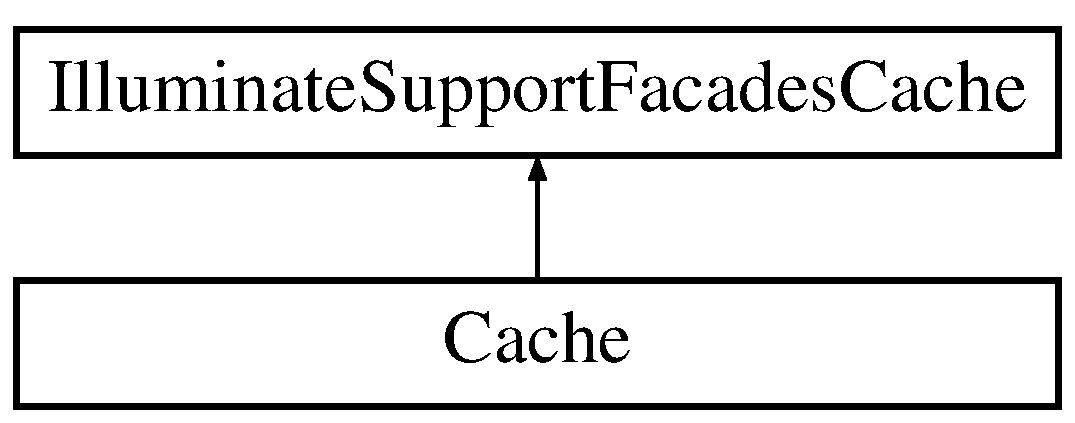
\includegraphics[height=2.000000cm]{class_cache}
\end{center}
\end{figure}
\subsection*{Additional Inherited Members}


The documentation for this class was generated from the following file\+:\begin{DoxyCompactItemize}
\item 
\+\_\+ide\+\_\+helper.\+php\end{DoxyCompactItemize}

\hypertarget{class_illuminate_1_1_support_1_1_facades_1_1_cache}{}\section{Illuminate\textbackslash{}Support\textbackslash{}Facades\textbackslash{}Cache Class Reference}
\label{class_illuminate_1_1_support_1_1_facades_1_1_cache}\index{Illuminate\textbackslash{}\+Support\textbackslash{}\+Facades\textbackslash{}\+Cache@{Illuminate\textbackslash{}\+Support\textbackslash{}\+Facades\textbackslash{}\+Cache}}
Inheritance diagram for Illuminate\textbackslash{}Support\textbackslash{}Facades\textbackslash{}Cache\+:\begin{figure}[H]
\begin{center}
\leavevmode
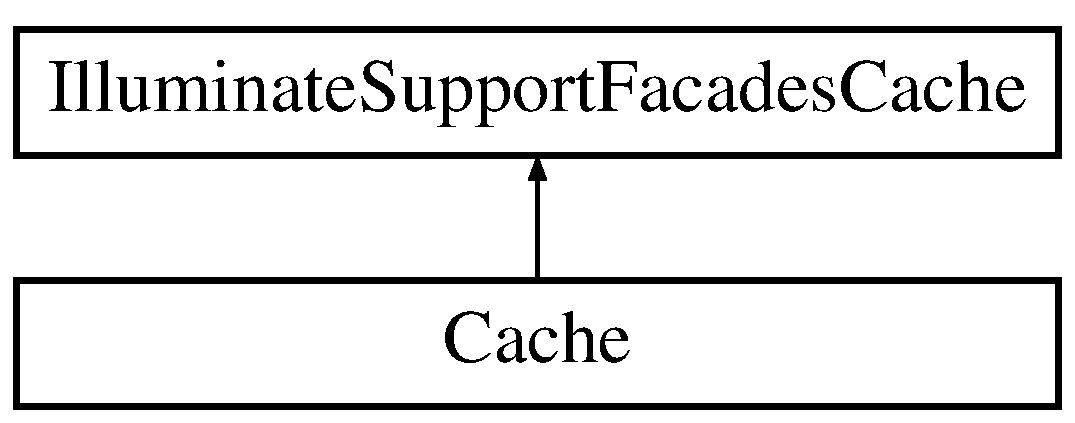
\includegraphics[height=2.000000cm]{class_illuminate_1_1_support_1_1_facades_1_1_cache}
\end{center}
\end{figure}
\subsection*{Static Public Member Functions}
\begin{DoxyCompactItemize}
\item 
static \mbox{\hyperlink{class_illuminate_1_1_support_1_1_facades_1_1_cache_a38e0420a18737d8cb49a6338174e58c5}{store}} (\$name=null)
\item 
static \mbox{\hyperlink{class_illuminate_1_1_support_1_1_facades_1_1_cache_afb69f3cc434ae38820079598349e543c}{driver}} (\$driver=null)
\item 
static \mbox{\hyperlink{class_illuminate_1_1_support_1_1_facades_1_1_cache_a85e3c1206e480386f4944aea0040b681}{repository}} (\$\mbox{\hyperlink{class_illuminate_1_1_support_1_1_facades_1_1_cache_a38e0420a18737d8cb49a6338174e58c5}{store}})
\item 
static \mbox{\hyperlink{class_illuminate_1_1_support_1_1_facades_1_1_cache_aefecc75567ab9855d949ddb8eaa434b5}{get\+Default\+Driver}} ()
\item 
static \mbox{\hyperlink{class_illuminate_1_1_support_1_1_facades_1_1_cache_a06a08b9ba638eb410c7e209092fa21bc}{set\+Default\+Driver}} (\$name)
\item 
static \mbox{\hyperlink{class_illuminate_1_1_support_1_1_facades_1_1_cache_a7ed3e4ef136849940ce40de0094563ef}{extend}} (\$\mbox{\hyperlink{class_illuminate_1_1_support_1_1_facades_1_1_cache_afb69f3cc434ae38820079598349e543c}{driver}}, \$callback)
\item 
static \mbox{\hyperlink{class_illuminate_1_1_support_1_1_facades_1_1_cache_af87ff499ffa620f8bf4a7e93571009e8}{has}} (\$key)
\item 
static \mbox{\hyperlink{class_illuminate_1_1_support_1_1_facades_1_1_cache_a470e91259e64ae2ba44cef45bece6234}{get}} (\$key, \$default=null)
\item 
static \mbox{\hyperlink{class_illuminate_1_1_support_1_1_facades_1_1_cache_ad164c41f53a86d42e3049cefc49cacb9}{many}} (\$keys)
\item 
static \mbox{\hyperlink{class_illuminate_1_1_support_1_1_facades_1_1_cache_a6ad46fca73497fd215a74a7edea74102}{get\+Multiple}} (\$keys, \$default=null)
\item 
static \mbox{\hyperlink{class_illuminate_1_1_support_1_1_facades_1_1_cache_a5d755e8df5b565d68fa8fbd88aa25a1a}{pull}} (\$key, \$default=null)
\item 
static \mbox{\hyperlink{class_illuminate_1_1_support_1_1_facades_1_1_cache_adda0a194865ce491f1beb2c92b3ab562}{put}} (\$key, \$value, \$minutes=null)
\item 
static \mbox{\hyperlink{class_illuminate_1_1_support_1_1_facades_1_1_cache_aae56ae54487230d52f542ccc1e44b9e0}{set}} (\$key, \$value, \$ttl=null)
\item 
static \mbox{\hyperlink{class_illuminate_1_1_support_1_1_facades_1_1_cache_a2e11599beb3fba7bafc407cdf87b0465}{put\+Many}} (\$values, \$minutes)
\item 
static \mbox{\hyperlink{class_illuminate_1_1_support_1_1_facades_1_1_cache_ae003e01cbfd273316452592dac9899cc}{set\+Multiple}} (\$values, \$ttl=null)
\item 
static \mbox{\hyperlink{class_illuminate_1_1_support_1_1_facades_1_1_cache_a5d3c1ec6a3f551739e6c3b360e48e938}{add}} (\$key, \$value, \$minutes)
\item 
static \mbox{\hyperlink{class_illuminate_1_1_support_1_1_facades_1_1_cache_ac922e6a2e98d1e8b294dc4d3988868b8}{increment}} (\$key, \$value=1)
\item 
static \mbox{\hyperlink{class_illuminate_1_1_support_1_1_facades_1_1_cache_a19a2ac21616577006738d270ebf66d1b}{decrement}} (\$key, \$value=1)
\item 
static \mbox{\hyperlink{class_illuminate_1_1_support_1_1_facades_1_1_cache_ad5857aecf260156120fb7cf288c0ae24}{forever}} (\$key, \$value)
\item 
static \mbox{\hyperlink{class_illuminate_1_1_support_1_1_facades_1_1_cache_aaa1f933dcd2732482b7818feb648fb5c}{remember}} (\$key, \$minutes, \$callback)
\item 
static \mbox{\hyperlink{class_illuminate_1_1_support_1_1_facades_1_1_cache_a2cd54fc860d738ed8388d33ee8bd05d4}{sear}} (\$key, \$callback)
\item 
static \mbox{\hyperlink{class_illuminate_1_1_support_1_1_facades_1_1_cache_a2e979a52ee4fdab7288c423516151a7a}{remember\+Forever}} (\$key, \$callback)
\item 
static \mbox{\hyperlink{class_illuminate_1_1_support_1_1_facades_1_1_cache_a95df8d5b2309d9b776fd3572273730b0}{forget}} (\$key)
\item 
static \mbox{\hyperlink{class_illuminate_1_1_support_1_1_facades_1_1_cache_a6a8c952c13ec741d6ce668652c9d42f9}{delete}} (\$key)
\item 
static \mbox{\hyperlink{class_illuminate_1_1_support_1_1_facades_1_1_cache_a9fbf5c08887ab8fec2eeab94a5ea09c3}{delete\+Multiple}} (\$keys)
\item 
static \mbox{\hyperlink{class_illuminate_1_1_support_1_1_facades_1_1_cache_a9928cda1869d6b3ea92ff1da3783ed36}{clear}} ()
\item 
static \mbox{\hyperlink{class_illuminate_1_1_support_1_1_facades_1_1_cache_a1d88420b147e30e153a7f22aeefc42a8}{tags}} (\$names)
\item 
static \mbox{\hyperlink{class_illuminate_1_1_support_1_1_facades_1_1_cache_ac00588a31484814762860326d0bd20a1}{get\+Default\+Cache\+Time}} ()
\item 
static \mbox{\hyperlink{class_illuminate_1_1_support_1_1_facades_1_1_cache_a778dc87a9a89af6e7efcaa6d264d3e4b}{set\+Default\+Cache\+Time}} (\$minutes)
\item 
static \mbox{\hyperlink{class_illuminate_1_1_support_1_1_facades_1_1_cache_a92e60124c2a55214d9692a14bdfa1083}{get\+Store}} ()
\item 
static \mbox{\hyperlink{class_illuminate_1_1_support_1_1_facades_1_1_cache_aac5b4b794ac19fbd44e66d46a9e298ba}{set\+Event\+Dispatcher}} (\$events)
\item 
static \mbox{\hyperlink{class_illuminate_1_1_support_1_1_facades_1_1_cache_a06b6deee91c4b1543fca7416885614f2}{offset\+Exists}} (\$key)
\item 
static \mbox{\hyperlink{class_illuminate_1_1_support_1_1_facades_1_1_cache_ac1f18c1895c1879f4759dfadbe63f7df}{offset\+Get}} (\$key)
\item 
static \mbox{\hyperlink{class_illuminate_1_1_support_1_1_facades_1_1_cache_a51056a380e3d655397251c75bbe34c79}{offset\+Set}} (\$key, \$value)
\item 
static \mbox{\hyperlink{class_illuminate_1_1_support_1_1_facades_1_1_cache_a41dc27b1a2a2ab6c69be0550627ebadf}{offset\+Unset}} (\$key)
\item 
static \mbox{\hyperlink{class_illuminate_1_1_support_1_1_facades_1_1_cache_a55a38c2032c537bbee8835736477e051}{macro}} (\$name, \$macro)
\item 
static \mbox{\hyperlink{class_illuminate_1_1_support_1_1_facades_1_1_cache_a7478b2077250bc5d8e79df6450914e55}{mixin}} (\$mixin)
\item 
static \mbox{\hyperlink{class_illuminate_1_1_support_1_1_facades_1_1_cache_ab77431154c802f667267725a67d81de9}{has\+Macro}} (\$name)
\item 
static \mbox{\hyperlink{class_illuminate_1_1_support_1_1_facades_1_1_cache_a6e137ad51d66f934dd10a880c36f1abb}{macro\+Call}} (\$method, \$parameters)
\item 
static \mbox{\hyperlink{class_illuminate_1_1_support_1_1_facades_1_1_cache_ad105f7d6cd0231543aeb58eea214149f}{flush}} ()
\item 
static \mbox{\hyperlink{class_illuminate_1_1_support_1_1_facades_1_1_cache_accbbacb3b8c964be370c343ec31724b2}{get\+Filesystem}} ()
\item 
static \mbox{\hyperlink{class_illuminate_1_1_support_1_1_facades_1_1_cache_a24345561ebd16cc82568f5d6dc32d753}{get\+Directory}} ()
\item 
static \mbox{\hyperlink{class_illuminate_1_1_support_1_1_facades_1_1_cache_aafd084ec4353419c5e807c1eac406bb4}{get\+Prefix}} ()
\end{DoxyCompactItemize}


\subsection{Member Function Documentation}
\mbox{\Hypertarget{class_illuminate_1_1_support_1_1_facades_1_1_cache_a5d3c1ec6a3f551739e6c3b360e48e938}\label{class_illuminate_1_1_support_1_1_facades_1_1_cache_a5d3c1ec6a3f551739e6c3b360e48e938}} 
\index{Illuminate\+::\+Support\+::\+Facades\+::\+Cache@{Illuminate\+::\+Support\+::\+Facades\+::\+Cache}!add@{add}}
\index{add@{add}!Illuminate\+::\+Support\+::\+Facades\+::\+Cache@{Illuminate\+::\+Support\+::\+Facades\+::\+Cache}}
\subsubsection{\texorpdfstring{add()}{add()}}
{\footnotesize\ttfamily static Illuminate\textbackslash{}\+Support\textbackslash{}\+Facades\textbackslash{}\+Cache\+::add (\begin{DoxyParamCaption}\item[{}]{\$key,  }\item[{}]{\$value,  }\item[{}]{\$minutes }\end{DoxyParamCaption})\hspace{0.3cm}{\ttfamily [static]}}

Store an item in the cache if the key does not exist.


\begin{DoxyParams}[1]{Parameters}
string & {\em \$key} & \\
\hline
mixed & {\em \$value} & \\
\hline
\textbackslash{}\+Date\+Time\+Interface | \textbackslash{}\+Date\+Interval | float | int & {\em \$minutes} & \\
\hline
\end{DoxyParams}
\begin{DoxyReturn}{Returns}
bool 
\end{DoxyReturn}
\mbox{\Hypertarget{class_illuminate_1_1_support_1_1_facades_1_1_cache_a9928cda1869d6b3ea92ff1da3783ed36}\label{class_illuminate_1_1_support_1_1_facades_1_1_cache_a9928cda1869d6b3ea92ff1da3783ed36}} 
\index{Illuminate\+::\+Support\+::\+Facades\+::\+Cache@{Illuminate\+::\+Support\+::\+Facades\+::\+Cache}!clear@{clear}}
\index{clear@{clear}!Illuminate\+::\+Support\+::\+Facades\+::\+Cache@{Illuminate\+::\+Support\+::\+Facades\+::\+Cache}}
\subsubsection{\texorpdfstring{clear()}{clear()}}
{\footnotesize\ttfamily static Illuminate\textbackslash{}\+Support\textbackslash{}\+Facades\textbackslash{}\+Cache\+::clear (\begin{DoxyParamCaption}{ }\end{DoxyParamCaption})\hspace{0.3cm}{\ttfamily [static]}}

Wipes clean the entire cache\textquotesingle{}s keys.

\begin{DoxyReturn}{Returns}
bool True on success and false on failure. 
\end{DoxyReturn}
\mbox{\Hypertarget{class_illuminate_1_1_support_1_1_facades_1_1_cache_a19a2ac21616577006738d270ebf66d1b}\label{class_illuminate_1_1_support_1_1_facades_1_1_cache_a19a2ac21616577006738d270ebf66d1b}} 
\index{Illuminate\+::\+Support\+::\+Facades\+::\+Cache@{Illuminate\+::\+Support\+::\+Facades\+::\+Cache}!decrement@{decrement}}
\index{decrement@{decrement}!Illuminate\+::\+Support\+::\+Facades\+::\+Cache@{Illuminate\+::\+Support\+::\+Facades\+::\+Cache}}
\subsubsection{\texorpdfstring{decrement()}{decrement()}}
{\footnotesize\ttfamily static Illuminate\textbackslash{}\+Support\textbackslash{}\+Facades\textbackslash{}\+Cache\+::decrement (\begin{DoxyParamCaption}\item[{}]{\$key,  }\item[{}]{\$value = {\ttfamily 1} }\end{DoxyParamCaption})\hspace{0.3cm}{\ttfamily [static]}}

Decrement the value of an item in the cache.


\begin{DoxyParams}[1]{Parameters}
string & {\em \$key} & \\
\hline
mixed & {\em \$value} & \\
\hline
\end{DoxyParams}
\begin{DoxyReturn}{Returns}
int$\vert$bool 
\end{DoxyReturn}
\mbox{\Hypertarget{class_illuminate_1_1_support_1_1_facades_1_1_cache_a6a8c952c13ec741d6ce668652c9d42f9}\label{class_illuminate_1_1_support_1_1_facades_1_1_cache_a6a8c952c13ec741d6ce668652c9d42f9}} 
\index{Illuminate\+::\+Support\+::\+Facades\+::\+Cache@{Illuminate\+::\+Support\+::\+Facades\+::\+Cache}!delete@{delete}}
\index{delete@{delete}!Illuminate\+::\+Support\+::\+Facades\+::\+Cache@{Illuminate\+::\+Support\+::\+Facades\+::\+Cache}}
\subsubsection{\texorpdfstring{delete()}{delete()}}
{\footnotesize\ttfamily static Illuminate\textbackslash{}\+Support\textbackslash{}\+Facades\textbackslash{}\+Cache\+::delete (\begin{DoxyParamCaption}\item[{}]{\$key }\end{DoxyParamCaption})\hspace{0.3cm}{\ttfamily [static]}}

Delete an item from the cache by its unique key.


\begin{DoxyParams}[1]{Parameters}
string & {\em \$key} & The unique cache key of the item to delete. \\
\hline
\end{DoxyParams}
\begin{DoxyReturn}{Returns}
bool True if the item was successfully removed. False if there was an error. 
\end{DoxyReturn}

\begin{DoxyExceptions}{Exceptions}
{\em } & \\
\hline
\end{DoxyExceptions}
\mbox{\Hypertarget{class_illuminate_1_1_support_1_1_facades_1_1_cache_a9fbf5c08887ab8fec2eeab94a5ea09c3}\label{class_illuminate_1_1_support_1_1_facades_1_1_cache_a9fbf5c08887ab8fec2eeab94a5ea09c3}} 
\index{Illuminate\+::\+Support\+::\+Facades\+::\+Cache@{Illuminate\+::\+Support\+::\+Facades\+::\+Cache}!delete\+Multiple@{delete\+Multiple}}
\index{delete\+Multiple@{delete\+Multiple}!Illuminate\+::\+Support\+::\+Facades\+::\+Cache@{Illuminate\+::\+Support\+::\+Facades\+::\+Cache}}
\subsubsection{\texorpdfstring{delete\+Multiple()}{deleteMultiple()}}
{\footnotesize\ttfamily static Illuminate\textbackslash{}\+Support\textbackslash{}\+Facades\textbackslash{}\+Cache\+::delete\+Multiple (\begin{DoxyParamCaption}\item[{}]{\$keys }\end{DoxyParamCaption})\hspace{0.3cm}{\ttfamily [static]}}

Deletes multiple cache items in a single operation.


\begin{DoxyParams}[1]{Parameters}
\textbackslash{}\+Psr\textbackslash{}\+Simple\+Cache\textbackslash{}iterable & {\em \$keys} & A list of string-\/based keys to be deleted. \\
\hline
\end{DoxyParams}
\begin{DoxyReturn}{Returns}
bool True if the items were successfully removed. False if there was an error. 
\end{DoxyReturn}

\begin{DoxyExceptions}{Exceptions}
{\em } & \\
\hline
\end{DoxyExceptions}
\mbox{\Hypertarget{class_illuminate_1_1_support_1_1_facades_1_1_cache_afb69f3cc434ae38820079598349e543c}\label{class_illuminate_1_1_support_1_1_facades_1_1_cache_afb69f3cc434ae38820079598349e543c}} 
\index{Illuminate\+::\+Support\+::\+Facades\+::\+Cache@{Illuminate\+::\+Support\+::\+Facades\+::\+Cache}!driver@{driver}}
\index{driver@{driver}!Illuminate\+::\+Support\+::\+Facades\+::\+Cache@{Illuminate\+::\+Support\+::\+Facades\+::\+Cache}}
\subsubsection{\texorpdfstring{driver()}{driver()}}
{\footnotesize\ttfamily static Illuminate\textbackslash{}\+Support\textbackslash{}\+Facades\textbackslash{}\+Cache\+::driver (\begin{DoxyParamCaption}\item[{}]{\$driver = {\ttfamily null} }\end{DoxyParamCaption})\hspace{0.3cm}{\ttfamily [static]}}

Get a cache driver instance.


\begin{DoxyParams}[1]{Parameters}
string & {\em \$driver} & \\
\hline
\end{DoxyParams}
\begin{DoxyReturn}{Returns}
mixed 
\end{DoxyReturn}
\mbox{\Hypertarget{class_illuminate_1_1_support_1_1_facades_1_1_cache_a7ed3e4ef136849940ce40de0094563ef}\label{class_illuminate_1_1_support_1_1_facades_1_1_cache_a7ed3e4ef136849940ce40de0094563ef}} 
\index{Illuminate\+::\+Support\+::\+Facades\+::\+Cache@{Illuminate\+::\+Support\+::\+Facades\+::\+Cache}!extend@{extend}}
\index{extend@{extend}!Illuminate\+::\+Support\+::\+Facades\+::\+Cache@{Illuminate\+::\+Support\+::\+Facades\+::\+Cache}}
\subsubsection{\texorpdfstring{extend()}{extend()}}
{\footnotesize\ttfamily static Illuminate\textbackslash{}\+Support\textbackslash{}\+Facades\textbackslash{}\+Cache\+::extend (\begin{DoxyParamCaption}\item[{}]{\$driver,  }\item[{}]{\$callback }\end{DoxyParamCaption})\hspace{0.3cm}{\ttfamily [static]}}

Register a custom driver creator Closure.


\begin{DoxyParams}[1]{Parameters}
string & {\em \$driver} & \\
\hline
\textbackslash{}\+Closure & {\em \$callback} & \\
\hline
\end{DoxyParams}
\begin{DoxyReturn}{Returns}
\$this 
\end{DoxyReturn}
\mbox{\Hypertarget{class_illuminate_1_1_support_1_1_facades_1_1_cache_ad105f7d6cd0231543aeb58eea214149f}\label{class_illuminate_1_1_support_1_1_facades_1_1_cache_ad105f7d6cd0231543aeb58eea214149f}} 
\index{Illuminate\+::\+Support\+::\+Facades\+::\+Cache@{Illuminate\+::\+Support\+::\+Facades\+::\+Cache}!flush@{flush}}
\index{flush@{flush}!Illuminate\+::\+Support\+::\+Facades\+::\+Cache@{Illuminate\+::\+Support\+::\+Facades\+::\+Cache}}
\subsubsection{\texorpdfstring{flush()}{flush()}}
{\footnotesize\ttfamily static Illuminate\textbackslash{}\+Support\textbackslash{}\+Facades\textbackslash{}\+Cache\+::flush (\begin{DoxyParamCaption}{ }\end{DoxyParamCaption})\hspace{0.3cm}{\ttfamily [static]}}

Remove all items from the cache.

\begin{DoxyReturn}{Returns}
bool 
\end{DoxyReturn}
\mbox{\Hypertarget{class_illuminate_1_1_support_1_1_facades_1_1_cache_ad5857aecf260156120fb7cf288c0ae24}\label{class_illuminate_1_1_support_1_1_facades_1_1_cache_ad5857aecf260156120fb7cf288c0ae24}} 
\index{Illuminate\+::\+Support\+::\+Facades\+::\+Cache@{Illuminate\+::\+Support\+::\+Facades\+::\+Cache}!forever@{forever}}
\index{forever@{forever}!Illuminate\+::\+Support\+::\+Facades\+::\+Cache@{Illuminate\+::\+Support\+::\+Facades\+::\+Cache}}
\subsubsection{\texorpdfstring{forever()}{forever()}}
{\footnotesize\ttfamily static Illuminate\textbackslash{}\+Support\textbackslash{}\+Facades\textbackslash{}\+Cache\+::forever (\begin{DoxyParamCaption}\item[{}]{\$key,  }\item[{}]{\$value }\end{DoxyParamCaption})\hspace{0.3cm}{\ttfamily [static]}}

Store an item in the cache indefinitely.


\begin{DoxyParams}[1]{Parameters}
string & {\em \$key} & \\
\hline
mixed & {\em \$value} & \\
\hline
\end{DoxyParams}
\begin{DoxyReturn}{Returns}
void 
\end{DoxyReturn}
\mbox{\Hypertarget{class_illuminate_1_1_support_1_1_facades_1_1_cache_a95df8d5b2309d9b776fd3572273730b0}\label{class_illuminate_1_1_support_1_1_facades_1_1_cache_a95df8d5b2309d9b776fd3572273730b0}} 
\index{Illuminate\+::\+Support\+::\+Facades\+::\+Cache@{Illuminate\+::\+Support\+::\+Facades\+::\+Cache}!forget@{forget}}
\index{forget@{forget}!Illuminate\+::\+Support\+::\+Facades\+::\+Cache@{Illuminate\+::\+Support\+::\+Facades\+::\+Cache}}
\subsubsection{\texorpdfstring{forget()}{forget()}}
{\footnotesize\ttfamily static Illuminate\textbackslash{}\+Support\textbackslash{}\+Facades\textbackslash{}\+Cache\+::forget (\begin{DoxyParamCaption}\item[{}]{\$key }\end{DoxyParamCaption})\hspace{0.3cm}{\ttfamily [static]}}

Remove an item from the cache.


\begin{DoxyParams}[1]{Parameters}
string & {\em \$key} & \\
\hline
\end{DoxyParams}
\begin{DoxyReturn}{Returns}
bool 
\end{DoxyReturn}
\mbox{\Hypertarget{class_illuminate_1_1_support_1_1_facades_1_1_cache_a470e91259e64ae2ba44cef45bece6234}\label{class_illuminate_1_1_support_1_1_facades_1_1_cache_a470e91259e64ae2ba44cef45bece6234}} 
\index{Illuminate\+::\+Support\+::\+Facades\+::\+Cache@{Illuminate\+::\+Support\+::\+Facades\+::\+Cache}!get@{get}}
\index{get@{get}!Illuminate\+::\+Support\+::\+Facades\+::\+Cache@{Illuminate\+::\+Support\+::\+Facades\+::\+Cache}}
\subsubsection{\texorpdfstring{get()}{get()}}
{\footnotesize\ttfamily static Illuminate\textbackslash{}\+Support\textbackslash{}\+Facades\textbackslash{}\+Cache\+::get (\begin{DoxyParamCaption}\item[{}]{\$key,  }\item[{}]{\$default = {\ttfamily null} }\end{DoxyParamCaption})\hspace{0.3cm}{\ttfamily [static]}}

Retrieve an item from the cache by key.


\begin{DoxyParams}[1]{Parameters}
string & {\em \$key} & \\
\hline
mixed & {\em \$default} & \\
\hline
\end{DoxyParams}
\begin{DoxyReturn}{Returns}
mixed 
\end{DoxyReturn}
\mbox{\Hypertarget{class_illuminate_1_1_support_1_1_facades_1_1_cache_ac00588a31484814762860326d0bd20a1}\label{class_illuminate_1_1_support_1_1_facades_1_1_cache_ac00588a31484814762860326d0bd20a1}} 
\index{Illuminate\+::\+Support\+::\+Facades\+::\+Cache@{Illuminate\+::\+Support\+::\+Facades\+::\+Cache}!get\+Default\+Cache\+Time@{get\+Default\+Cache\+Time}}
\index{get\+Default\+Cache\+Time@{get\+Default\+Cache\+Time}!Illuminate\+::\+Support\+::\+Facades\+::\+Cache@{Illuminate\+::\+Support\+::\+Facades\+::\+Cache}}
\subsubsection{\texorpdfstring{get\+Default\+Cache\+Time()}{getDefaultCacheTime()}}
{\footnotesize\ttfamily static Illuminate\textbackslash{}\+Support\textbackslash{}\+Facades\textbackslash{}\+Cache\+::get\+Default\+Cache\+Time (\begin{DoxyParamCaption}{ }\end{DoxyParamCaption})\hspace{0.3cm}{\ttfamily [static]}}

Get the default cache time.

\begin{DoxyReturn}{Returns}
float$\vert$int 
\end{DoxyReturn}
\mbox{\Hypertarget{class_illuminate_1_1_support_1_1_facades_1_1_cache_aefecc75567ab9855d949ddb8eaa434b5}\label{class_illuminate_1_1_support_1_1_facades_1_1_cache_aefecc75567ab9855d949ddb8eaa434b5}} 
\index{Illuminate\+::\+Support\+::\+Facades\+::\+Cache@{Illuminate\+::\+Support\+::\+Facades\+::\+Cache}!get\+Default\+Driver@{get\+Default\+Driver}}
\index{get\+Default\+Driver@{get\+Default\+Driver}!Illuminate\+::\+Support\+::\+Facades\+::\+Cache@{Illuminate\+::\+Support\+::\+Facades\+::\+Cache}}
\subsubsection{\texorpdfstring{get\+Default\+Driver()}{getDefaultDriver()}}
{\footnotesize\ttfamily static Illuminate\textbackslash{}\+Support\textbackslash{}\+Facades\textbackslash{}\+Cache\+::get\+Default\+Driver (\begin{DoxyParamCaption}{ }\end{DoxyParamCaption})\hspace{0.3cm}{\ttfamily [static]}}

Get the default cache driver name.

\begin{DoxyReturn}{Returns}
string 
\end{DoxyReturn}
\mbox{\Hypertarget{class_illuminate_1_1_support_1_1_facades_1_1_cache_a24345561ebd16cc82568f5d6dc32d753}\label{class_illuminate_1_1_support_1_1_facades_1_1_cache_a24345561ebd16cc82568f5d6dc32d753}} 
\index{Illuminate\+::\+Support\+::\+Facades\+::\+Cache@{Illuminate\+::\+Support\+::\+Facades\+::\+Cache}!get\+Directory@{get\+Directory}}
\index{get\+Directory@{get\+Directory}!Illuminate\+::\+Support\+::\+Facades\+::\+Cache@{Illuminate\+::\+Support\+::\+Facades\+::\+Cache}}
\subsubsection{\texorpdfstring{get\+Directory()}{getDirectory()}}
{\footnotesize\ttfamily static Illuminate\textbackslash{}\+Support\textbackslash{}\+Facades\textbackslash{}\+Cache\+::get\+Directory (\begin{DoxyParamCaption}{ }\end{DoxyParamCaption})\hspace{0.3cm}{\ttfamily [static]}}

Get the working directory of the cache.

\begin{DoxyReturn}{Returns}
string 
\end{DoxyReturn}
\mbox{\Hypertarget{class_illuminate_1_1_support_1_1_facades_1_1_cache_accbbacb3b8c964be370c343ec31724b2}\label{class_illuminate_1_1_support_1_1_facades_1_1_cache_accbbacb3b8c964be370c343ec31724b2}} 
\index{Illuminate\+::\+Support\+::\+Facades\+::\+Cache@{Illuminate\+::\+Support\+::\+Facades\+::\+Cache}!get\+Filesystem@{get\+Filesystem}}
\index{get\+Filesystem@{get\+Filesystem}!Illuminate\+::\+Support\+::\+Facades\+::\+Cache@{Illuminate\+::\+Support\+::\+Facades\+::\+Cache}}
\subsubsection{\texorpdfstring{get\+Filesystem()}{getFilesystem()}}
{\footnotesize\ttfamily static Illuminate\textbackslash{}\+Support\textbackslash{}\+Facades\textbackslash{}\+Cache\+::get\+Filesystem (\begin{DoxyParamCaption}{ }\end{DoxyParamCaption})\hspace{0.3cm}{\ttfamily [static]}}

Get the Filesystem instance.

\begin{DoxyReturn}{Returns}

\end{DoxyReturn}
\mbox{\Hypertarget{class_illuminate_1_1_support_1_1_facades_1_1_cache_a6ad46fca73497fd215a74a7edea74102}\label{class_illuminate_1_1_support_1_1_facades_1_1_cache_a6ad46fca73497fd215a74a7edea74102}} 
\index{Illuminate\+::\+Support\+::\+Facades\+::\+Cache@{Illuminate\+::\+Support\+::\+Facades\+::\+Cache}!get\+Multiple@{get\+Multiple}}
\index{get\+Multiple@{get\+Multiple}!Illuminate\+::\+Support\+::\+Facades\+::\+Cache@{Illuminate\+::\+Support\+::\+Facades\+::\+Cache}}
\subsubsection{\texorpdfstring{get\+Multiple()}{getMultiple()}}
{\footnotesize\ttfamily static Illuminate\textbackslash{}\+Support\textbackslash{}\+Facades\textbackslash{}\+Cache\+::get\+Multiple (\begin{DoxyParamCaption}\item[{}]{\$keys,  }\item[{}]{\$default = {\ttfamily null} }\end{DoxyParamCaption})\hspace{0.3cm}{\ttfamily [static]}}

Obtains multiple cache items by their unique keys.


\begin{DoxyParams}[1]{Parameters}
\textbackslash{}\+Psr\textbackslash{}\+Simple\+Cache\textbackslash{}iterable & {\em \$keys} & A list of keys that can obtained in a single operation. \\
\hline
mixed & {\em \$default} & Default value to return for keys that do not exist. \\
\hline
\end{DoxyParams}
\begin{DoxyReturn}{Returns}
A list of key =$>$ value pairs. \mbox{\hyperlink{class_illuminate_1_1_support_1_1_facades_1_1_cache}{Cache}} keys that do not exist or are stale will have \$default as value. 
\end{DoxyReturn}

\begin{DoxyExceptions}{Exceptions}
{\em } & \\
\hline
\end{DoxyExceptions}
\mbox{\Hypertarget{class_illuminate_1_1_support_1_1_facades_1_1_cache_aafd084ec4353419c5e807c1eac406bb4}\label{class_illuminate_1_1_support_1_1_facades_1_1_cache_aafd084ec4353419c5e807c1eac406bb4}} 
\index{Illuminate\+::\+Support\+::\+Facades\+::\+Cache@{Illuminate\+::\+Support\+::\+Facades\+::\+Cache}!get\+Prefix@{get\+Prefix}}
\index{get\+Prefix@{get\+Prefix}!Illuminate\+::\+Support\+::\+Facades\+::\+Cache@{Illuminate\+::\+Support\+::\+Facades\+::\+Cache}}
\subsubsection{\texorpdfstring{get\+Prefix()}{getPrefix()}}
{\footnotesize\ttfamily static Illuminate\textbackslash{}\+Support\textbackslash{}\+Facades\textbackslash{}\+Cache\+::get\+Prefix (\begin{DoxyParamCaption}{ }\end{DoxyParamCaption})\hspace{0.3cm}{\ttfamily [static]}}

Get the cache key prefix.

\begin{DoxyReturn}{Returns}
string 
\end{DoxyReturn}
\mbox{\Hypertarget{class_illuminate_1_1_support_1_1_facades_1_1_cache_a92e60124c2a55214d9692a14bdfa1083}\label{class_illuminate_1_1_support_1_1_facades_1_1_cache_a92e60124c2a55214d9692a14bdfa1083}} 
\index{Illuminate\+::\+Support\+::\+Facades\+::\+Cache@{Illuminate\+::\+Support\+::\+Facades\+::\+Cache}!get\+Store@{get\+Store}}
\index{get\+Store@{get\+Store}!Illuminate\+::\+Support\+::\+Facades\+::\+Cache@{Illuminate\+::\+Support\+::\+Facades\+::\+Cache}}
\subsubsection{\texorpdfstring{get\+Store()}{getStore()}}
{\footnotesize\ttfamily static Illuminate\textbackslash{}\+Support\textbackslash{}\+Facades\textbackslash{}\+Cache\+::get\+Store (\begin{DoxyParamCaption}{ }\end{DoxyParamCaption})\hspace{0.3cm}{\ttfamily [static]}}

Get the cache store implementation.

\begin{DoxyReturn}{Returns}

\end{DoxyReturn}
\mbox{\Hypertarget{class_illuminate_1_1_support_1_1_facades_1_1_cache_af87ff499ffa620f8bf4a7e93571009e8}\label{class_illuminate_1_1_support_1_1_facades_1_1_cache_af87ff499ffa620f8bf4a7e93571009e8}} 
\index{Illuminate\+::\+Support\+::\+Facades\+::\+Cache@{Illuminate\+::\+Support\+::\+Facades\+::\+Cache}!has@{has}}
\index{has@{has}!Illuminate\+::\+Support\+::\+Facades\+::\+Cache@{Illuminate\+::\+Support\+::\+Facades\+::\+Cache}}
\subsubsection{\texorpdfstring{has()}{has()}}
{\footnotesize\ttfamily static Illuminate\textbackslash{}\+Support\textbackslash{}\+Facades\textbackslash{}\+Cache\+::has (\begin{DoxyParamCaption}\item[{}]{\$key }\end{DoxyParamCaption})\hspace{0.3cm}{\ttfamily [static]}}

Determine if an item exists in the cache.


\begin{DoxyParams}[1]{Parameters}
string & {\em \$key} & \\
\hline
\end{DoxyParams}
\begin{DoxyReturn}{Returns}
bool 
\end{DoxyReturn}
\mbox{\Hypertarget{class_illuminate_1_1_support_1_1_facades_1_1_cache_ab77431154c802f667267725a67d81de9}\label{class_illuminate_1_1_support_1_1_facades_1_1_cache_ab77431154c802f667267725a67d81de9}} 
\index{Illuminate\+::\+Support\+::\+Facades\+::\+Cache@{Illuminate\+::\+Support\+::\+Facades\+::\+Cache}!has\+Macro@{has\+Macro}}
\index{has\+Macro@{has\+Macro}!Illuminate\+::\+Support\+::\+Facades\+::\+Cache@{Illuminate\+::\+Support\+::\+Facades\+::\+Cache}}
\subsubsection{\texorpdfstring{has\+Macro()}{hasMacro()}}
{\footnotesize\ttfamily static Illuminate\textbackslash{}\+Support\textbackslash{}\+Facades\textbackslash{}\+Cache\+::has\+Macro (\begin{DoxyParamCaption}\item[{}]{\$name }\end{DoxyParamCaption})\hspace{0.3cm}{\ttfamily [static]}}

Checks if macro is registered.


\begin{DoxyParams}[1]{Parameters}
string & {\em \$name} & \\
\hline
\end{DoxyParams}
\begin{DoxyReturn}{Returns}
bool 
\end{DoxyReturn}
\mbox{\Hypertarget{class_illuminate_1_1_support_1_1_facades_1_1_cache_ac922e6a2e98d1e8b294dc4d3988868b8}\label{class_illuminate_1_1_support_1_1_facades_1_1_cache_ac922e6a2e98d1e8b294dc4d3988868b8}} 
\index{Illuminate\+::\+Support\+::\+Facades\+::\+Cache@{Illuminate\+::\+Support\+::\+Facades\+::\+Cache}!increment@{increment}}
\index{increment@{increment}!Illuminate\+::\+Support\+::\+Facades\+::\+Cache@{Illuminate\+::\+Support\+::\+Facades\+::\+Cache}}
\subsubsection{\texorpdfstring{increment()}{increment()}}
{\footnotesize\ttfamily static Illuminate\textbackslash{}\+Support\textbackslash{}\+Facades\textbackslash{}\+Cache\+::increment (\begin{DoxyParamCaption}\item[{}]{\$key,  }\item[{}]{\$value = {\ttfamily 1} }\end{DoxyParamCaption})\hspace{0.3cm}{\ttfamily [static]}}

Increment the value of an item in the cache.


\begin{DoxyParams}[1]{Parameters}
string & {\em \$key} & \\
\hline
mixed & {\em \$value} & \\
\hline
\end{DoxyParams}
\begin{DoxyReturn}{Returns}
int$\vert$bool 
\end{DoxyReturn}
\mbox{\Hypertarget{class_illuminate_1_1_support_1_1_facades_1_1_cache_a55a38c2032c537bbee8835736477e051}\label{class_illuminate_1_1_support_1_1_facades_1_1_cache_a55a38c2032c537bbee8835736477e051}} 
\index{Illuminate\+::\+Support\+::\+Facades\+::\+Cache@{Illuminate\+::\+Support\+::\+Facades\+::\+Cache}!macro@{macro}}
\index{macro@{macro}!Illuminate\+::\+Support\+::\+Facades\+::\+Cache@{Illuminate\+::\+Support\+::\+Facades\+::\+Cache}}
\subsubsection{\texorpdfstring{macro()}{macro()}}
{\footnotesize\ttfamily static Illuminate\textbackslash{}\+Support\textbackslash{}\+Facades\textbackslash{}\+Cache\+::macro (\begin{DoxyParamCaption}\item[{}]{\$name,  }\item[{}]{\$macro }\end{DoxyParamCaption})\hspace{0.3cm}{\ttfamily [static]}}

Register a custom macro.


\begin{DoxyParams}[1]{Parameters}
string & {\em \$name} & \\
\hline
object | callable & {\em \$macro} & \\
\hline
\end{DoxyParams}
\begin{DoxyReturn}{Returns}
void 
\end{DoxyReturn}
\mbox{\Hypertarget{class_illuminate_1_1_support_1_1_facades_1_1_cache_a6e137ad51d66f934dd10a880c36f1abb}\label{class_illuminate_1_1_support_1_1_facades_1_1_cache_a6e137ad51d66f934dd10a880c36f1abb}} 
\index{Illuminate\+::\+Support\+::\+Facades\+::\+Cache@{Illuminate\+::\+Support\+::\+Facades\+::\+Cache}!macro\+Call@{macro\+Call}}
\index{macro\+Call@{macro\+Call}!Illuminate\+::\+Support\+::\+Facades\+::\+Cache@{Illuminate\+::\+Support\+::\+Facades\+::\+Cache}}
\subsubsection{\texorpdfstring{macro\+Call()}{macroCall()}}
{\footnotesize\ttfamily static Illuminate\textbackslash{}\+Support\textbackslash{}\+Facades\textbackslash{}\+Cache\+::macro\+Call (\begin{DoxyParamCaption}\item[{}]{\$method,  }\item[{}]{\$parameters }\end{DoxyParamCaption})\hspace{0.3cm}{\ttfamily [static]}}

Dynamically handle calls to the class.


\begin{DoxyParams}[1]{Parameters}
string & {\em \$method} & \\
\hline
array & {\em \$parameters} & \\
\hline
\end{DoxyParams}
\begin{DoxyReturn}{Returns}
mixed 
\end{DoxyReturn}

\begin{DoxyExceptions}{Exceptions}
{\em } & \\
\hline
\end{DoxyExceptions}
\mbox{\Hypertarget{class_illuminate_1_1_support_1_1_facades_1_1_cache_ad164c41f53a86d42e3049cefc49cacb9}\label{class_illuminate_1_1_support_1_1_facades_1_1_cache_ad164c41f53a86d42e3049cefc49cacb9}} 
\index{Illuminate\+::\+Support\+::\+Facades\+::\+Cache@{Illuminate\+::\+Support\+::\+Facades\+::\+Cache}!many@{many}}
\index{many@{many}!Illuminate\+::\+Support\+::\+Facades\+::\+Cache@{Illuminate\+::\+Support\+::\+Facades\+::\+Cache}}
\subsubsection{\texorpdfstring{many()}{many()}}
{\footnotesize\ttfamily static Illuminate\textbackslash{}\+Support\textbackslash{}\+Facades\textbackslash{}\+Cache\+::many (\begin{DoxyParamCaption}\item[{}]{\$keys }\end{DoxyParamCaption})\hspace{0.3cm}{\ttfamily [static]}}

Retrieve multiple items from the cache by key.

Items not found in the cache will have a null value.


\begin{DoxyParams}[1]{Parameters}
array & {\em \$keys} & \\
\hline
\end{DoxyParams}
\begin{DoxyReturn}{Returns}
array 
\end{DoxyReturn}
\mbox{\Hypertarget{class_illuminate_1_1_support_1_1_facades_1_1_cache_a7478b2077250bc5d8e79df6450914e55}\label{class_illuminate_1_1_support_1_1_facades_1_1_cache_a7478b2077250bc5d8e79df6450914e55}} 
\index{Illuminate\+::\+Support\+::\+Facades\+::\+Cache@{Illuminate\+::\+Support\+::\+Facades\+::\+Cache}!mixin@{mixin}}
\index{mixin@{mixin}!Illuminate\+::\+Support\+::\+Facades\+::\+Cache@{Illuminate\+::\+Support\+::\+Facades\+::\+Cache}}
\subsubsection{\texorpdfstring{mixin()}{mixin()}}
{\footnotesize\ttfamily static Illuminate\textbackslash{}\+Support\textbackslash{}\+Facades\textbackslash{}\+Cache\+::mixin (\begin{DoxyParamCaption}\item[{}]{\$mixin }\end{DoxyParamCaption})\hspace{0.3cm}{\ttfamily [static]}}

Mix another object into the class.


\begin{DoxyParams}[1]{Parameters}
object & {\em \$mixin} & \\
\hline
\end{DoxyParams}
\begin{DoxyReturn}{Returns}
void 
\end{DoxyReturn}
\mbox{\Hypertarget{class_illuminate_1_1_support_1_1_facades_1_1_cache_a06b6deee91c4b1543fca7416885614f2}\label{class_illuminate_1_1_support_1_1_facades_1_1_cache_a06b6deee91c4b1543fca7416885614f2}} 
\index{Illuminate\+::\+Support\+::\+Facades\+::\+Cache@{Illuminate\+::\+Support\+::\+Facades\+::\+Cache}!offset\+Exists@{offset\+Exists}}
\index{offset\+Exists@{offset\+Exists}!Illuminate\+::\+Support\+::\+Facades\+::\+Cache@{Illuminate\+::\+Support\+::\+Facades\+::\+Cache}}
\subsubsection{\texorpdfstring{offset\+Exists()}{offsetExists()}}
{\footnotesize\ttfamily static Illuminate\textbackslash{}\+Support\textbackslash{}\+Facades\textbackslash{}\+Cache\+::offset\+Exists (\begin{DoxyParamCaption}\item[{}]{\$key }\end{DoxyParamCaption})\hspace{0.3cm}{\ttfamily [static]}}

Determine if a cached value exists.


\begin{DoxyParams}[1]{Parameters}
string & {\em \$key} & \\
\hline
\end{DoxyParams}
\begin{DoxyReturn}{Returns}
bool 
\end{DoxyReturn}
\mbox{\Hypertarget{class_illuminate_1_1_support_1_1_facades_1_1_cache_ac1f18c1895c1879f4759dfadbe63f7df}\label{class_illuminate_1_1_support_1_1_facades_1_1_cache_ac1f18c1895c1879f4759dfadbe63f7df}} 
\index{Illuminate\+::\+Support\+::\+Facades\+::\+Cache@{Illuminate\+::\+Support\+::\+Facades\+::\+Cache}!offset\+Get@{offset\+Get}}
\index{offset\+Get@{offset\+Get}!Illuminate\+::\+Support\+::\+Facades\+::\+Cache@{Illuminate\+::\+Support\+::\+Facades\+::\+Cache}}
\subsubsection{\texorpdfstring{offset\+Get()}{offsetGet()}}
{\footnotesize\ttfamily static Illuminate\textbackslash{}\+Support\textbackslash{}\+Facades\textbackslash{}\+Cache\+::offset\+Get (\begin{DoxyParamCaption}\item[{}]{\$key }\end{DoxyParamCaption})\hspace{0.3cm}{\ttfamily [static]}}

Retrieve an item from the cache by key.


\begin{DoxyParams}[1]{Parameters}
string & {\em \$key} & \\
\hline
\end{DoxyParams}
\begin{DoxyReturn}{Returns}
mixed 
\end{DoxyReturn}
\mbox{\Hypertarget{class_illuminate_1_1_support_1_1_facades_1_1_cache_a51056a380e3d655397251c75bbe34c79}\label{class_illuminate_1_1_support_1_1_facades_1_1_cache_a51056a380e3d655397251c75bbe34c79}} 
\index{Illuminate\+::\+Support\+::\+Facades\+::\+Cache@{Illuminate\+::\+Support\+::\+Facades\+::\+Cache}!offset\+Set@{offset\+Set}}
\index{offset\+Set@{offset\+Set}!Illuminate\+::\+Support\+::\+Facades\+::\+Cache@{Illuminate\+::\+Support\+::\+Facades\+::\+Cache}}
\subsubsection{\texorpdfstring{offset\+Set()}{offsetSet()}}
{\footnotesize\ttfamily static Illuminate\textbackslash{}\+Support\textbackslash{}\+Facades\textbackslash{}\+Cache\+::offset\+Set (\begin{DoxyParamCaption}\item[{}]{\$key,  }\item[{}]{\$value }\end{DoxyParamCaption})\hspace{0.3cm}{\ttfamily [static]}}

Store an item in the cache for the default time.


\begin{DoxyParams}[1]{Parameters}
string & {\em \$key} & \\
\hline
mixed & {\em \$value} & \\
\hline
\end{DoxyParams}
\begin{DoxyReturn}{Returns}
void 
\end{DoxyReturn}
\mbox{\Hypertarget{class_illuminate_1_1_support_1_1_facades_1_1_cache_a41dc27b1a2a2ab6c69be0550627ebadf}\label{class_illuminate_1_1_support_1_1_facades_1_1_cache_a41dc27b1a2a2ab6c69be0550627ebadf}} 
\index{Illuminate\+::\+Support\+::\+Facades\+::\+Cache@{Illuminate\+::\+Support\+::\+Facades\+::\+Cache}!offset\+Unset@{offset\+Unset}}
\index{offset\+Unset@{offset\+Unset}!Illuminate\+::\+Support\+::\+Facades\+::\+Cache@{Illuminate\+::\+Support\+::\+Facades\+::\+Cache}}
\subsubsection{\texorpdfstring{offset\+Unset()}{offsetUnset()}}
{\footnotesize\ttfamily static Illuminate\textbackslash{}\+Support\textbackslash{}\+Facades\textbackslash{}\+Cache\+::offset\+Unset (\begin{DoxyParamCaption}\item[{}]{\$key }\end{DoxyParamCaption})\hspace{0.3cm}{\ttfamily [static]}}

Remove an item from the cache.


\begin{DoxyParams}[1]{Parameters}
string & {\em \$key} & \\
\hline
\end{DoxyParams}
\begin{DoxyReturn}{Returns}
void 
\end{DoxyReturn}
\mbox{\Hypertarget{class_illuminate_1_1_support_1_1_facades_1_1_cache_a5d755e8df5b565d68fa8fbd88aa25a1a}\label{class_illuminate_1_1_support_1_1_facades_1_1_cache_a5d755e8df5b565d68fa8fbd88aa25a1a}} 
\index{Illuminate\+::\+Support\+::\+Facades\+::\+Cache@{Illuminate\+::\+Support\+::\+Facades\+::\+Cache}!pull@{pull}}
\index{pull@{pull}!Illuminate\+::\+Support\+::\+Facades\+::\+Cache@{Illuminate\+::\+Support\+::\+Facades\+::\+Cache}}
\subsubsection{\texorpdfstring{pull()}{pull()}}
{\footnotesize\ttfamily static Illuminate\textbackslash{}\+Support\textbackslash{}\+Facades\textbackslash{}\+Cache\+::pull (\begin{DoxyParamCaption}\item[{}]{\$key,  }\item[{}]{\$default = {\ttfamily null} }\end{DoxyParamCaption})\hspace{0.3cm}{\ttfamily [static]}}

Retrieve an item from the cache and delete it.


\begin{DoxyParams}[1]{Parameters}
string & {\em \$key} & \\
\hline
mixed & {\em \$default} & \\
\hline
\end{DoxyParams}
\begin{DoxyReturn}{Returns}
mixed 
\end{DoxyReturn}
\mbox{\Hypertarget{class_illuminate_1_1_support_1_1_facades_1_1_cache_adda0a194865ce491f1beb2c92b3ab562}\label{class_illuminate_1_1_support_1_1_facades_1_1_cache_adda0a194865ce491f1beb2c92b3ab562}} 
\index{Illuminate\+::\+Support\+::\+Facades\+::\+Cache@{Illuminate\+::\+Support\+::\+Facades\+::\+Cache}!put@{put}}
\index{put@{put}!Illuminate\+::\+Support\+::\+Facades\+::\+Cache@{Illuminate\+::\+Support\+::\+Facades\+::\+Cache}}
\subsubsection{\texorpdfstring{put()}{put()}}
{\footnotesize\ttfamily static Illuminate\textbackslash{}\+Support\textbackslash{}\+Facades\textbackslash{}\+Cache\+::put (\begin{DoxyParamCaption}\item[{}]{\$key,  }\item[{}]{\$value,  }\item[{}]{\$minutes = {\ttfamily null} }\end{DoxyParamCaption})\hspace{0.3cm}{\ttfamily [static]}}

Store an item in the cache.


\begin{DoxyParams}[1]{Parameters}
string & {\em \$key} & \\
\hline
mixed & {\em \$value} & \\
\hline
\textbackslash{}\+Date\+Time\+Interface | \textbackslash{}\+Date\+Interval | float | int & {\em \$minutes} & \\
\hline
\end{DoxyParams}
\begin{DoxyReturn}{Returns}
void 
\end{DoxyReturn}
\mbox{\Hypertarget{class_illuminate_1_1_support_1_1_facades_1_1_cache_a2e11599beb3fba7bafc407cdf87b0465}\label{class_illuminate_1_1_support_1_1_facades_1_1_cache_a2e11599beb3fba7bafc407cdf87b0465}} 
\index{Illuminate\+::\+Support\+::\+Facades\+::\+Cache@{Illuminate\+::\+Support\+::\+Facades\+::\+Cache}!put\+Many@{put\+Many}}
\index{put\+Many@{put\+Many}!Illuminate\+::\+Support\+::\+Facades\+::\+Cache@{Illuminate\+::\+Support\+::\+Facades\+::\+Cache}}
\subsubsection{\texorpdfstring{put\+Many()}{putMany()}}
{\footnotesize\ttfamily static Illuminate\textbackslash{}\+Support\textbackslash{}\+Facades\textbackslash{}\+Cache\+::put\+Many (\begin{DoxyParamCaption}\item[{}]{\$values,  }\item[{}]{\$minutes }\end{DoxyParamCaption})\hspace{0.3cm}{\ttfamily [static]}}

Store multiple items in the cache for a given number of minutes.


\begin{DoxyParams}[1]{Parameters}
array & {\em \$values} & \\
\hline
\textbackslash{}\+Date\+Time\+Interface | \textbackslash{}\+Date\+Interval | float | int & {\em \$minutes} & \\
\hline
\end{DoxyParams}
\begin{DoxyReturn}{Returns}
void 
\end{DoxyReturn}
\mbox{\Hypertarget{class_illuminate_1_1_support_1_1_facades_1_1_cache_aaa1f933dcd2732482b7818feb648fb5c}\label{class_illuminate_1_1_support_1_1_facades_1_1_cache_aaa1f933dcd2732482b7818feb648fb5c}} 
\index{Illuminate\+::\+Support\+::\+Facades\+::\+Cache@{Illuminate\+::\+Support\+::\+Facades\+::\+Cache}!remember@{remember}}
\index{remember@{remember}!Illuminate\+::\+Support\+::\+Facades\+::\+Cache@{Illuminate\+::\+Support\+::\+Facades\+::\+Cache}}
\subsubsection{\texorpdfstring{remember()}{remember()}}
{\footnotesize\ttfamily static Illuminate\textbackslash{}\+Support\textbackslash{}\+Facades\textbackslash{}\+Cache\+::remember (\begin{DoxyParamCaption}\item[{}]{\$key,  }\item[{}]{\$minutes,  }\item[{}]{\$callback }\end{DoxyParamCaption})\hspace{0.3cm}{\ttfamily [static]}}

Get an item from the cache, or store the default value.


\begin{DoxyParams}[1]{Parameters}
string & {\em \$key} & \\
\hline
\textbackslash{}\+Date\+Time\+Interface | \textbackslash{}\+Date\+Interval | float | int & {\em \$minutes} & \\
\hline
\textbackslash{}\+Closure & {\em \$callback} & \\
\hline
\end{DoxyParams}
\begin{DoxyReturn}{Returns}
mixed 
\end{DoxyReturn}
\mbox{\Hypertarget{class_illuminate_1_1_support_1_1_facades_1_1_cache_a2e979a52ee4fdab7288c423516151a7a}\label{class_illuminate_1_1_support_1_1_facades_1_1_cache_a2e979a52ee4fdab7288c423516151a7a}} 
\index{Illuminate\+::\+Support\+::\+Facades\+::\+Cache@{Illuminate\+::\+Support\+::\+Facades\+::\+Cache}!remember\+Forever@{remember\+Forever}}
\index{remember\+Forever@{remember\+Forever}!Illuminate\+::\+Support\+::\+Facades\+::\+Cache@{Illuminate\+::\+Support\+::\+Facades\+::\+Cache}}
\subsubsection{\texorpdfstring{remember\+Forever()}{rememberForever()}}
{\footnotesize\ttfamily static Illuminate\textbackslash{}\+Support\textbackslash{}\+Facades\textbackslash{}\+Cache\+::remember\+Forever (\begin{DoxyParamCaption}\item[{}]{\$key,  }\item[{}]{\$callback }\end{DoxyParamCaption})\hspace{0.3cm}{\ttfamily [static]}}

Get an item from the cache, or store the default value forever.


\begin{DoxyParams}[1]{Parameters}
string & {\em \$key} & \\
\hline
\textbackslash{}\+Closure & {\em \$callback} & \\
\hline
\end{DoxyParams}
\begin{DoxyReturn}{Returns}
mixed 
\end{DoxyReturn}
\mbox{\Hypertarget{class_illuminate_1_1_support_1_1_facades_1_1_cache_a85e3c1206e480386f4944aea0040b681}\label{class_illuminate_1_1_support_1_1_facades_1_1_cache_a85e3c1206e480386f4944aea0040b681}} 
\index{Illuminate\+::\+Support\+::\+Facades\+::\+Cache@{Illuminate\+::\+Support\+::\+Facades\+::\+Cache}!repository@{repository}}
\index{repository@{repository}!Illuminate\+::\+Support\+::\+Facades\+::\+Cache@{Illuminate\+::\+Support\+::\+Facades\+::\+Cache}}
\subsubsection{\texorpdfstring{repository()}{repository()}}
{\footnotesize\ttfamily static Illuminate\textbackslash{}\+Support\textbackslash{}\+Facades\textbackslash{}\+Cache\+::repository (\begin{DoxyParamCaption}\item[{}]{\$store }\end{DoxyParamCaption})\hspace{0.3cm}{\ttfamily [static]}}

Create a new cache repository with the given implementation.


\begin{DoxyParams}[1]{Parameters}
\textbackslash{}\+Illuminate\textbackslash{}\+Contracts\textbackslash{}\+Cache\textbackslash{}\+Store & {\em \$store} & \\
\hline
\end{DoxyParams}
\begin{DoxyReturn}{Returns}

\end{DoxyReturn}
\mbox{\Hypertarget{class_illuminate_1_1_support_1_1_facades_1_1_cache_a2cd54fc860d738ed8388d33ee8bd05d4}\label{class_illuminate_1_1_support_1_1_facades_1_1_cache_a2cd54fc860d738ed8388d33ee8bd05d4}} 
\index{Illuminate\+::\+Support\+::\+Facades\+::\+Cache@{Illuminate\+::\+Support\+::\+Facades\+::\+Cache}!sear@{sear}}
\index{sear@{sear}!Illuminate\+::\+Support\+::\+Facades\+::\+Cache@{Illuminate\+::\+Support\+::\+Facades\+::\+Cache}}
\subsubsection{\texorpdfstring{sear()}{sear()}}
{\footnotesize\ttfamily static Illuminate\textbackslash{}\+Support\textbackslash{}\+Facades\textbackslash{}\+Cache\+::sear (\begin{DoxyParamCaption}\item[{}]{\$key,  }\item[{}]{\$callback }\end{DoxyParamCaption})\hspace{0.3cm}{\ttfamily [static]}}

Get an item from the cache, or store the default value forever.


\begin{DoxyParams}[1]{Parameters}
string & {\em \$key} & \\
\hline
\textbackslash{}\+Closure & {\em \$callback} & \\
\hline
\end{DoxyParams}
\begin{DoxyReturn}{Returns}
mixed 
\end{DoxyReturn}
\mbox{\Hypertarget{class_illuminate_1_1_support_1_1_facades_1_1_cache_aae56ae54487230d52f542ccc1e44b9e0}\label{class_illuminate_1_1_support_1_1_facades_1_1_cache_aae56ae54487230d52f542ccc1e44b9e0}} 
\index{Illuminate\+::\+Support\+::\+Facades\+::\+Cache@{Illuminate\+::\+Support\+::\+Facades\+::\+Cache}!set@{set}}
\index{set@{set}!Illuminate\+::\+Support\+::\+Facades\+::\+Cache@{Illuminate\+::\+Support\+::\+Facades\+::\+Cache}}
\subsubsection{\texorpdfstring{set()}{set()}}
{\footnotesize\ttfamily static Illuminate\textbackslash{}\+Support\textbackslash{}\+Facades\textbackslash{}\+Cache\+::set (\begin{DoxyParamCaption}\item[{}]{\$key,  }\item[{}]{\$value,  }\item[{}]{\$ttl = {\ttfamily null} }\end{DoxyParamCaption})\hspace{0.3cm}{\ttfamily [static]}}

Persists data in the cache, uniquely referenced by a key with an optional expiration T\+TL time.


\begin{DoxyParams}[1]{Parameters}
string & {\em \$key} & The key of the item to store. \\
\hline
mixed & {\em \$value} & The value of the item to store, must be serializable. \\
\hline
null | int | \textbackslash{}\+Date\+Interval & {\em \$ttl} & Optional. The T\+TL value of this item. If no value is sent and the driver supports T\+TL then the library may set a default value for it or let the driver take care of that. \\
\hline
\end{DoxyParams}
\begin{DoxyReturn}{Returns}
bool True on success and false on failure. 
\end{DoxyReturn}

\begin{DoxyExceptions}{Exceptions}
{\em } & \\
\hline
\end{DoxyExceptions}
\mbox{\Hypertarget{class_illuminate_1_1_support_1_1_facades_1_1_cache_a778dc87a9a89af6e7efcaa6d264d3e4b}\label{class_illuminate_1_1_support_1_1_facades_1_1_cache_a778dc87a9a89af6e7efcaa6d264d3e4b}} 
\index{Illuminate\+::\+Support\+::\+Facades\+::\+Cache@{Illuminate\+::\+Support\+::\+Facades\+::\+Cache}!set\+Default\+Cache\+Time@{set\+Default\+Cache\+Time}}
\index{set\+Default\+Cache\+Time@{set\+Default\+Cache\+Time}!Illuminate\+::\+Support\+::\+Facades\+::\+Cache@{Illuminate\+::\+Support\+::\+Facades\+::\+Cache}}
\subsubsection{\texorpdfstring{set\+Default\+Cache\+Time()}{setDefaultCacheTime()}}
{\footnotesize\ttfamily static Illuminate\textbackslash{}\+Support\textbackslash{}\+Facades\textbackslash{}\+Cache\+::set\+Default\+Cache\+Time (\begin{DoxyParamCaption}\item[{}]{\$minutes }\end{DoxyParamCaption})\hspace{0.3cm}{\ttfamily [static]}}

Set the default cache time in minutes.


\begin{DoxyParams}[1]{Parameters}
float | int & {\em \$minutes} & \\
\hline
\end{DoxyParams}
\begin{DoxyReturn}{Returns}
\$this 
\end{DoxyReturn}
\mbox{\Hypertarget{class_illuminate_1_1_support_1_1_facades_1_1_cache_a06a08b9ba638eb410c7e209092fa21bc}\label{class_illuminate_1_1_support_1_1_facades_1_1_cache_a06a08b9ba638eb410c7e209092fa21bc}} 
\index{Illuminate\+::\+Support\+::\+Facades\+::\+Cache@{Illuminate\+::\+Support\+::\+Facades\+::\+Cache}!set\+Default\+Driver@{set\+Default\+Driver}}
\index{set\+Default\+Driver@{set\+Default\+Driver}!Illuminate\+::\+Support\+::\+Facades\+::\+Cache@{Illuminate\+::\+Support\+::\+Facades\+::\+Cache}}
\subsubsection{\texorpdfstring{set\+Default\+Driver()}{setDefaultDriver()}}
{\footnotesize\ttfamily static Illuminate\textbackslash{}\+Support\textbackslash{}\+Facades\textbackslash{}\+Cache\+::set\+Default\+Driver (\begin{DoxyParamCaption}\item[{}]{\$name }\end{DoxyParamCaption})\hspace{0.3cm}{\ttfamily [static]}}

Set the default cache driver name.


\begin{DoxyParams}[1]{Parameters}
string & {\em \$name} & \\
\hline
\end{DoxyParams}
\begin{DoxyReturn}{Returns}
void 
\end{DoxyReturn}
\mbox{\Hypertarget{class_illuminate_1_1_support_1_1_facades_1_1_cache_aac5b4b794ac19fbd44e66d46a9e298ba}\label{class_illuminate_1_1_support_1_1_facades_1_1_cache_aac5b4b794ac19fbd44e66d46a9e298ba}} 
\index{Illuminate\+::\+Support\+::\+Facades\+::\+Cache@{Illuminate\+::\+Support\+::\+Facades\+::\+Cache}!set\+Event\+Dispatcher@{set\+Event\+Dispatcher}}
\index{set\+Event\+Dispatcher@{set\+Event\+Dispatcher}!Illuminate\+::\+Support\+::\+Facades\+::\+Cache@{Illuminate\+::\+Support\+::\+Facades\+::\+Cache}}
\subsubsection{\texorpdfstring{set\+Event\+Dispatcher()}{setEventDispatcher()}}
{\footnotesize\ttfamily static Illuminate\textbackslash{}\+Support\textbackslash{}\+Facades\textbackslash{}\+Cache\+::set\+Event\+Dispatcher (\begin{DoxyParamCaption}\item[{}]{\$events }\end{DoxyParamCaption})\hspace{0.3cm}{\ttfamily [static]}}

Set the event dispatcher instance.


\begin{DoxyParams}[1]{Parameters}
\textbackslash{}\+Illuminate\textbackslash{}\+Contracts\textbackslash{}\+Events\textbackslash{}\+Dispatcher & {\em \$events} & \\
\hline
\end{DoxyParams}
\begin{DoxyReturn}{Returns}
void 
\end{DoxyReturn}
\mbox{\Hypertarget{class_illuminate_1_1_support_1_1_facades_1_1_cache_ae003e01cbfd273316452592dac9899cc}\label{class_illuminate_1_1_support_1_1_facades_1_1_cache_ae003e01cbfd273316452592dac9899cc}} 
\index{Illuminate\+::\+Support\+::\+Facades\+::\+Cache@{Illuminate\+::\+Support\+::\+Facades\+::\+Cache}!set\+Multiple@{set\+Multiple}}
\index{set\+Multiple@{set\+Multiple}!Illuminate\+::\+Support\+::\+Facades\+::\+Cache@{Illuminate\+::\+Support\+::\+Facades\+::\+Cache}}
\subsubsection{\texorpdfstring{set\+Multiple()}{setMultiple()}}
{\footnotesize\ttfamily static Illuminate\textbackslash{}\+Support\textbackslash{}\+Facades\textbackslash{}\+Cache\+::set\+Multiple (\begin{DoxyParamCaption}\item[{}]{\$values,  }\item[{}]{\$ttl = {\ttfamily null} }\end{DoxyParamCaption})\hspace{0.3cm}{\ttfamily [static]}}

Persists a set of key =$>$ value pairs in the cache, with an optional T\+TL.


\begin{DoxyParams}[1]{Parameters}
\textbackslash{}\+Psr\textbackslash{}\+Simple\+Cache\textbackslash{}iterable & {\em \$values} & A list of key =$>$ value pairs for a multiple-\/set operation. \\
\hline
null | int | \textbackslash{}\+Date\+Interval & {\em \$ttl} & Optional. The T\+TL value of this item. If no value is sent and the driver supports T\+TL then the library may set a default value for it or let the driver take care of that. \\
\hline
\end{DoxyParams}
\begin{DoxyReturn}{Returns}
bool True on success and false on failure. 
\end{DoxyReturn}

\begin{DoxyExceptions}{Exceptions}
{\em } & \\
\hline
\end{DoxyExceptions}
\mbox{\Hypertarget{class_illuminate_1_1_support_1_1_facades_1_1_cache_a38e0420a18737d8cb49a6338174e58c5}\label{class_illuminate_1_1_support_1_1_facades_1_1_cache_a38e0420a18737d8cb49a6338174e58c5}} 
\index{Illuminate\+::\+Support\+::\+Facades\+::\+Cache@{Illuminate\+::\+Support\+::\+Facades\+::\+Cache}!store@{store}}
\index{store@{store}!Illuminate\+::\+Support\+::\+Facades\+::\+Cache@{Illuminate\+::\+Support\+::\+Facades\+::\+Cache}}
\subsubsection{\texorpdfstring{store()}{store()}}
{\footnotesize\ttfamily static Illuminate\textbackslash{}\+Support\textbackslash{}\+Facades\textbackslash{}\+Cache\+::store (\begin{DoxyParamCaption}\item[{}]{\$name = {\ttfamily null} }\end{DoxyParamCaption})\hspace{0.3cm}{\ttfamily [static]}}

Get a cache store instance by name.


\begin{DoxyParams}[1]{Parameters}
string | null & {\em \$name} & \\
\hline
\end{DoxyParams}
\begin{DoxyReturn}{Returns}

\end{DoxyReturn}
\mbox{\Hypertarget{class_illuminate_1_1_support_1_1_facades_1_1_cache_a1d88420b147e30e153a7f22aeefc42a8}\label{class_illuminate_1_1_support_1_1_facades_1_1_cache_a1d88420b147e30e153a7f22aeefc42a8}} 
\index{Illuminate\+::\+Support\+::\+Facades\+::\+Cache@{Illuminate\+::\+Support\+::\+Facades\+::\+Cache}!tags@{tags}}
\index{tags@{tags}!Illuminate\+::\+Support\+::\+Facades\+::\+Cache@{Illuminate\+::\+Support\+::\+Facades\+::\+Cache}}
\subsubsection{\texorpdfstring{tags()}{tags()}}
{\footnotesize\ttfamily static Illuminate\textbackslash{}\+Support\textbackslash{}\+Facades\textbackslash{}\+Cache\+::tags (\begin{DoxyParamCaption}\item[{}]{\$names }\end{DoxyParamCaption})\hspace{0.3cm}{\ttfamily [static]}}

Begin executing a new tags operation if the store supports it.


\begin{DoxyParams}[1]{Parameters}
array | mixed & {\em \$names} & \\
\hline
\end{DoxyParams}
\begin{DoxyReturn}{Returns}

\end{DoxyReturn}

\begin{DoxyExceptions}{Exceptions}
{\em } & \\
\hline
\end{DoxyExceptions}


The documentation for this class was generated from the following file\+:\begin{DoxyCompactItemize}
\item 
\+\_\+ide\+\_\+helper.\+php\end{DoxyCompactItemize}

\hypertarget{class_illuminate_1_1_support_1_1_facades_1_1_config}{}\section{Illuminate\textbackslash{}Support\textbackslash{}Facades\textbackslash{}Config Class Reference}
\label{class_illuminate_1_1_support_1_1_facades_1_1_config}\index{Illuminate\textbackslash{}\+Support\textbackslash{}\+Facades\textbackslash{}\+Config@{Illuminate\textbackslash{}\+Support\textbackslash{}\+Facades\textbackslash{}\+Config}}
Inheritance diagram for Illuminate\textbackslash{}Support\textbackslash{}Facades\textbackslash{}Config\+:\begin{figure}[H]
\begin{center}
\leavevmode
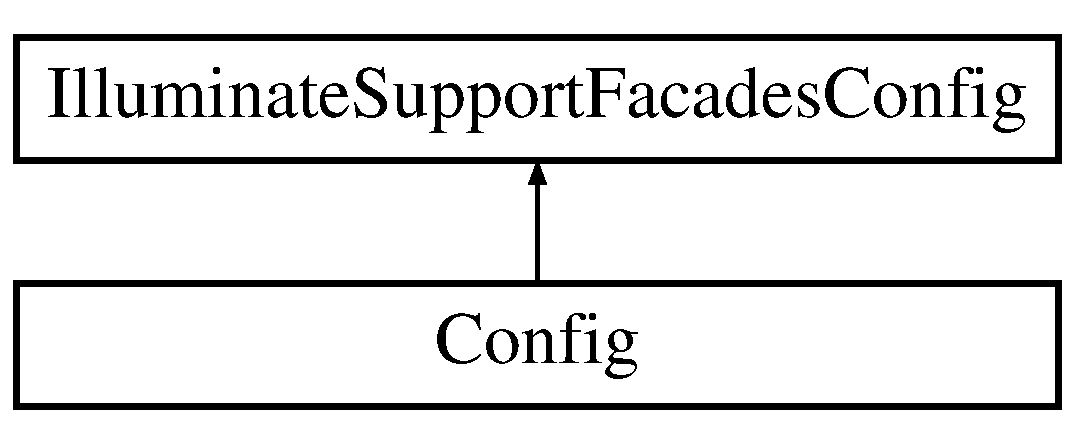
\includegraphics[height=2.000000cm]{class_illuminate_1_1_support_1_1_facades_1_1_config}
\end{center}
\end{figure}
\subsection*{Static Public Member Functions}
\begin{DoxyCompactItemize}
\item 
static \mbox{\hyperlink{class_illuminate_1_1_support_1_1_facades_1_1_config_ae0f1ddeede4ff756dadd4b6048c25888}{has}} (\$key)
\item 
static \mbox{\hyperlink{class_illuminate_1_1_support_1_1_facades_1_1_config_ac5241c47a6ee12cf3694dfde287a282e}{get}} (\$key, \$default=null)
\item 
static \mbox{\hyperlink{class_illuminate_1_1_support_1_1_facades_1_1_config_ab45caadb7b699ed2b74ce3b5b148f016}{get\+Many}} (\$keys)
\item 
static \mbox{\hyperlink{class_illuminate_1_1_support_1_1_facades_1_1_config_a7047f1890e3395145ad9653dd05e5091}{set}} (\$key, \$value=null)
\item 
static \mbox{\hyperlink{class_illuminate_1_1_support_1_1_facades_1_1_config_a2bd99f6f5d1781a64670f54279695e74}{prepend}} (\$key, \$value)
\item 
static \mbox{\hyperlink{class_illuminate_1_1_support_1_1_facades_1_1_config_a9e793f445e2052cc39b7529f9d865398}{push}} (\$key, \$value)
\item 
static \mbox{\hyperlink{class_illuminate_1_1_support_1_1_facades_1_1_config_a3e96fa02210901a504f5d6cecbb3058b}{all}} ()
\item 
static \mbox{\hyperlink{class_illuminate_1_1_support_1_1_facades_1_1_config_a9c38dfaca860625f3f3ec57ba2d94f62}{offset\+Exists}} (\$key)
\item 
static \mbox{\hyperlink{class_illuminate_1_1_support_1_1_facades_1_1_config_aafef797ee6d2b5dd5fb4c152015da9c4}{offset\+Get}} (\$key)
\item 
static \mbox{\hyperlink{class_illuminate_1_1_support_1_1_facades_1_1_config_ac8f6afca8969d60e4e3aab883debcaee}{offset\+Set}} (\$key, \$value)
\item 
static \mbox{\hyperlink{class_illuminate_1_1_support_1_1_facades_1_1_config_a5238463d5080f7a8bcd7a75ef481c4f5}{offset\+Unset}} (\$key)
\end{DoxyCompactItemize}


\subsection{Member Function Documentation}
\mbox{\Hypertarget{class_illuminate_1_1_support_1_1_facades_1_1_config_a3e96fa02210901a504f5d6cecbb3058b}\label{class_illuminate_1_1_support_1_1_facades_1_1_config_a3e96fa02210901a504f5d6cecbb3058b}} 
\index{Illuminate\+::\+Support\+::\+Facades\+::\+Config@{Illuminate\+::\+Support\+::\+Facades\+::\+Config}!all@{all}}
\index{all@{all}!Illuminate\+::\+Support\+::\+Facades\+::\+Config@{Illuminate\+::\+Support\+::\+Facades\+::\+Config}}
\subsubsection{\texorpdfstring{all()}{all()}}
{\footnotesize\ttfamily static Illuminate\textbackslash{}\+Support\textbackslash{}\+Facades\textbackslash{}\+Config\+::all (\begin{DoxyParamCaption}{ }\end{DoxyParamCaption})\hspace{0.3cm}{\ttfamily [static]}}

Get all of the configuration items for the application.

\begin{DoxyReturn}{Returns}
array 
\end{DoxyReturn}
\mbox{\Hypertarget{class_illuminate_1_1_support_1_1_facades_1_1_config_ac5241c47a6ee12cf3694dfde287a282e}\label{class_illuminate_1_1_support_1_1_facades_1_1_config_ac5241c47a6ee12cf3694dfde287a282e}} 
\index{Illuminate\+::\+Support\+::\+Facades\+::\+Config@{Illuminate\+::\+Support\+::\+Facades\+::\+Config}!get@{get}}
\index{get@{get}!Illuminate\+::\+Support\+::\+Facades\+::\+Config@{Illuminate\+::\+Support\+::\+Facades\+::\+Config}}
\subsubsection{\texorpdfstring{get()}{get()}}
{\footnotesize\ttfamily static Illuminate\textbackslash{}\+Support\textbackslash{}\+Facades\textbackslash{}\+Config\+::get (\begin{DoxyParamCaption}\item[{}]{\$key,  }\item[{}]{\$default = {\ttfamily null} }\end{DoxyParamCaption})\hspace{0.3cm}{\ttfamily [static]}}

Get the specified configuration value.


\begin{DoxyParams}[1]{Parameters}
array | string & {\em \$key} & \\
\hline
mixed & {\em \$default} & \\
\hline
\end{DoxyParams}
\begin{DoxyReturn}{Returns}
mixed 
\end{DoxyReturn}
\mbox{\Hypertarget{class_illuminate_1_1_support_1_1_facades_1_1_config_ab45caadb7b699ed2b74ce3b5b148f016}\label{class_illuminate_1_1_support_1_1_facades_1_1_config_ab45caadb7b699ed2b74ce3b5b148f016}} 
\index{Illuminate\+::\+Support\+::\+Facades\+::\+Config@{Illuminate\+::\+Support\+::\+Facades\+::\+Config}!get\+Many@{get\+Many}}
\index{get\+Many@{get\+Many}!Illuminate\+::\+Support\+::\+Facades\+::\+Config@{Illuminate\+::\+Support\+::\+Facades\+::\+Config}}
\subsubsection{\texorpdfstring{get\+Many()}{getMany()}}
{\footnotesize\ttfamily static Illuminate\textbackslash{}\+Support\textbackslash{}\+Facades\textbackslash{}\+Config\+::get\+Many (\begin{DoxyParamCaption}\item[{}]{\$keys }\end{DoxyParamCaption})\hspace{0.3cm}{\ttfamily [static]}}

Get many configuration values.


\begin{DoxyParams}[1]{Parameters}
array & {\em \$keys} & \\
\hline
\end{DoxyParams}
\begin{DoxyReturn}{Returns}
array 
\end{DoxyReturn}
\mbox{\Hypertarget{class_illuminate_1_1_support_1_1_facades_1_1_config_ae0f1ddeede4ff756dadd4b6048c25888}\label{class_illuminate_1_1_support_1_1_facades_1_1_config_ae0f1ddeede4ff756dadd4b6048c25888}} 
\index{Illuminate\+::\+Support\+::\+Facades\+::\+Config@{Illuminate\+::\+Support\+::\+Facades\+::\+Config}!has@{has}}
\index{has@{has}!Illuminate\+::\+Support\+::\+Facades\+::\+Config@{Illuminate\+::\+Support\+::\+Facades\+::\+Config}}
\subsubsection{\texorpdfstring{has()}{has()}}
{\footnotesize\ttfamily static Illuminate\textbackslash{}\+Support\textbackslash{}\+Facades\textbackslash{}\+Config\+::has (\begin{DoxyParamCaption}\item[{}]{\$key }\end{DoxyParamCaption})\hspace{0.3cm}{\ttfamily [static]}}

Determine if the given configuration value exists.


\begin{DoxyParams}[1]{Parameters}
string & {\em \$key} & \\
\hline
\end{DoxyParams}
\begin{DoxyReturn}{Returns}
bool 
\end{DoxyReturn}
\mbox{\Hypertarget{class_illuminate_1_1_support_1_1_facades_1_1_config_a9c38dfaca860625f3f3ec57ba2d94f62}\label{class_illuminate_1_1_support_1_1_facades_1_1_config_a9c38dfaca860625f3f3ec57ba2d94f62}} 
\index{Illuminate\+::\+Support\+::\+Facades\+::\+Config@{Illuminate\+::\+Support\+::\+Facades\+::\+Config}!offset\+Exists@{offset\+Exists}}
\index{offset\+Exists@{offset\+Exists}!Illuminate\+::\+Support\+::\+Facades\+::\+Config@{Illuminate\+::\+Support\+::\+Facades\+::\+Config}}
\subsubsection{\texorpdfstring{offset\+Exists()}{offsetExists()}}
{\footnotesize\ttfamily static Illuminate\textbackslash{}\+Support\textbackslash{}\+Facades\textbackslash{}\+Config\+::offset\+Exists (\begin{DoxyParamCaption}\item[{}]{\$key }\end{DoxyParamCaption})\hspace{0.3cm}{\ttfamily [static]}}

Determine if the given configuration option exists.


\begin{DoxyParams}[1]{Parameters}
string & {\em \$key} & \\
\hline
\end{DoxyParams}
\begin{DoxyReturn}{Returns}
bool 
\end{DoxyReturn}
\mbox{\Hypertarget{class_illuminate_1_1_support_1_1_facades_1_1_config_aafef797ee6d2b5dd5fb4c152015da9c4}\label{class_illuminate_1_1_support_1_1_facades_1_1_config_aafef797ee6d2b5dd5fb4c152015da9c4}} 
\index{Illuminate\+::\+Support\+::\+Facades\+::\+Config@{Illuminate\+::\+Support\+::\+Facades\+::\+Config}!offset\+Get@{offset\+Get}}
\index{offset\+Get@{offset\+Get}!Illuminate\+::\+Support\+::\+Facades\+::\+Config@{Illuminate\+::\+Support\+::\+Facades\+::\+Config}}
\subsubsection{\texorpdfstring{offset\+Get()}{offsetGet()}}
{\footnotesize\ttfamily static Illuminate\textbackslash{}\+Support\textbackslash{}\+Facades\textbackslash{}\+Config\+::offset\+Get (\begin{DoxyParamCaption}\item[{}]{\$key }\end{DoxyParamCaption})\hspace{0.3cm}{\ttfamily [static]}}

Get a configuration option.


\begin{DoxyParams}[1]{Parameters}
string & {\em \$key} & \\
\hline
\end{DoxyParams}
\begin{DoxyReturn}{Returns}
mixed 
\end{DoxyReturn}
\mbox{\Hypertarget{class_illuminate_1_1_support_1_1_facades_1_1_config_ac8f6afca8969d60e4e3aab883debcaee}\label{class_illuminate_1_1_support_1_1_facades_1_1_config_ac8f6afca8969d60e4e3aab883debcaee}} 
\index{Illuminate\+::\+Support\+::\+Facades\+::\+Config@{Illuminate\+::\+Support\+::\+Facades\+::\+Config}!offset\+Set@{offset\+Set}}
\index{offset\+Set@{offset\+Set}!Illuminate\+::\+Support\+::\+Facades\+::\+Config@{Illuminate\+::\+Support\+::\+Facades\+::\+Config}}
\subsubsection{\texorpdfstring{offset\+Set()}{offsetSet()}}
{\footnotesize\ttfamily static Illuminate\textbackslash{}\+Support\textbackslash{}\+Facades\textbackslash{}\+Config\+::offset\+Set (\begin{DoxyParamCaption}\item[{}]{\$key,  }\item[{}]{\$value }\end{DoxyParamCaption})\hspace{0.3cm}{\ttfamily [static]}}

Set a configuration option.


\begin{DoxyParams}[1]{Parameters}
string & {\em \$key} & \\
\hline
mixed & {\em \$value} & \\
\hline
\end{DoxyParams}
\begin{DoxyReturn}{Returns}
void 
\end{DoxyReturn}
\mbox{\Hypertarget{class_illuminate_1_1_support_1_1_facades_1_1_config_a5238463d5080f7a8bcd7a75ef481c4f5}\label{class_illuminate_1_1_support_1_1_facades_1_1_config_a5238463d5080f7a8bcd7a75ef481c4f5}} 
\index{Illuminate\+::\+Support\+::\+Facades\+::\+Config@{Illuminate\+::\+Support\+::\+Facades\+::\+Config}!offset\+Unset@{offset\+Unset}}
\index{offset\+Unset@{offset\+Unset}!Illuminate\+::\+Support\+::\+Facades\+::\+Config@{Illuminate\+::\+Support\+::\+Facades\+::\+Config}}
\subsubsection{\texorpdfstring{offset\+Unset()}{offsetUnset()}}
{\footnotesize\ttfamily static Illuminate\textbackslash{}\+Support\textbackslash{}\+Facades\textbackslash{}\+Config\+::offset\+Unset (\begin{DoxyParamCaption}\item[{}]{\$key }\end{DoxyParamCaption})\hspace{0.3cm}{\ttfamily [static]}}

Unset a configuration option.


\begin{DoxyParams}[1]{Parameters}
string & {\em \$key} & \\
\hline
\end{DoxyParams}
\begin{DoxyReturn}{Returns}
void 
\end{DoxyReturn}
\mbox{\Hypertarget{class_illuminate_1_1_support_1_1_facades_1_1_config_a2bd99f6f5d1781a64670f54279695e74}\label{class_illuminate_1_1_support_1_1_facades_1_1_config_a2bd99f6f5d1781a64670f54279695e74}} 
\index{Illuminate\+::\+Support\+::\+Facades\+::\+Config@{Illuminate\+::\+Support\+::\+Facades\+::\+Config}!prepend@{prepend}}
\index{prepend@{prepend}!Illuminate\+::\+Support\+::\+Facades\+::\+Config@{Illuminate\+::\+Support\+::\+Facades\+::\+Config}}
\subsubsection{\texorpdfstring{prepend()}{prepend()}}
{\footnotesize\ttfamily static Illuminate\textbackslash{}\+Support\textbackslash{}\+Facades\textbackslash{}\+Config\+::prepend (\begin{DoxyParamCaption}\item[{}]{\$key,  }\item[{}]{\$value }\end{DoxyParamCaption})\hspace{0.3cm}{\ttfamily [static]}}

Prepend a value onto an array configuration value.


\begin{DoxyParams}[1]{Parameters}
string & {\em \$key} & \\
\hline
mixed & {\em \$value} & \\
\hline
\end{DoxyParams}
\begin{DoxyReturn}{Returns}
void 
\end{DoxyReturn}
\mbox{\Hypertarget{class_illuminate_1_1_support_1_1_facades_1_1_config_a9e793f445e2052cc39b7529f9d865398}\label{class_illuminate_1_1_support_1_1_facades_1_1_config_a9e793f445e2052cc39b7529f9d865398}} 
\index{Illuminate\+::\+Support\+::\+Facades\+::\+Config@{Illuminate\+::\+Support\+::\+Facades\+::\+Config}!push@{push}}
\index{push@{push}!Illuminate\+::\+Support\+::\+Facades\+::\+Config@{Illuminate\+::\+Support\+::\+Facades\+::\+Config}}
\subsubsection{\texorpdfstring{push()}{push()}}
{\footnotesize\ttfamily static Illuminate\textbackslash{}\+Support\textbackslash{}\+Facades\textbackslash{}\+Config\+::push (\begin{DoxyParamCaption}\item[{}]{\$key,  }\item[{}]{\$value }\end{DoxyParamCaption})\hspace{0.3cm}{\ttfamily [static]}}

Push a value onto an array configuration value.


\begin{DoxyParams}[1]{Parameters}
string & {\em \$key} & \\
\hline
mixed & {\em \$value} & \\
\hline
\end{DoxyParams}
\begin{DoxyReturn}{Returns}
void 
\end{DoxyReturn}
\mbox{\Hypertarget{class_illuminate_1_1_support_1_1_facades_1_1_config_a7047f1890e3395145ad9653dd05e5091}\label{class_illuminate_1_1_support_1_1_facades_1_1_config_a7047f1890e3395145ad9653dd05e5091}} 
\index{Illuminate\+::\+Support\+::\+Facades\+::\+Config@{Illuminate\+::\+Support\+::\+Facades\+::\+Config}!set@{set}}
\index{set@{set}!Illuminate\+::\+Support\+::\+Facades\+::\+Config@{Illuminate\+::\+Support\+::\+Facades\+::\+Config}}
\subsubsection{\texorpdfstring{set()}{set()}}
{\footnotesize\ttfamily static Illuminate\textbackslash{}\+Support\textbackslash{}\+Facades\textbackslash{}\+Config\+::set (\begin{DoxyParamCaption}\item[{}]{\$key,  }\item[{}]{\$value = {\ttfamily null} }\end{DoxyParamCaption})\hspace{0.3cm}{\ttfamily [static]}}

Set a given configuration value.


\begin{DoxyParams}[1]{Parameters}
array | string & {\em \$key} & \\
\hline
mixed & {\em \$value} & \\
\hline
\end{DoxyParams}
\begin{DoxyReturn}{Returns}
void 
\end{DoxyReturn}


The documentation for this class was generated from the following file\+:\begin{DoxyCompactItemize}
\item 
\+\_\+ide\+\_\+helper.\+php\end{DoxyCompactItemize}

\hypertarget{class_config}{}\section{Config Class Reference}
\label{class_config}\index{Config@{Config}}
Inheritance diagram for Config\+:\begin{figure}[H]
\begin{center}
\leavevmode
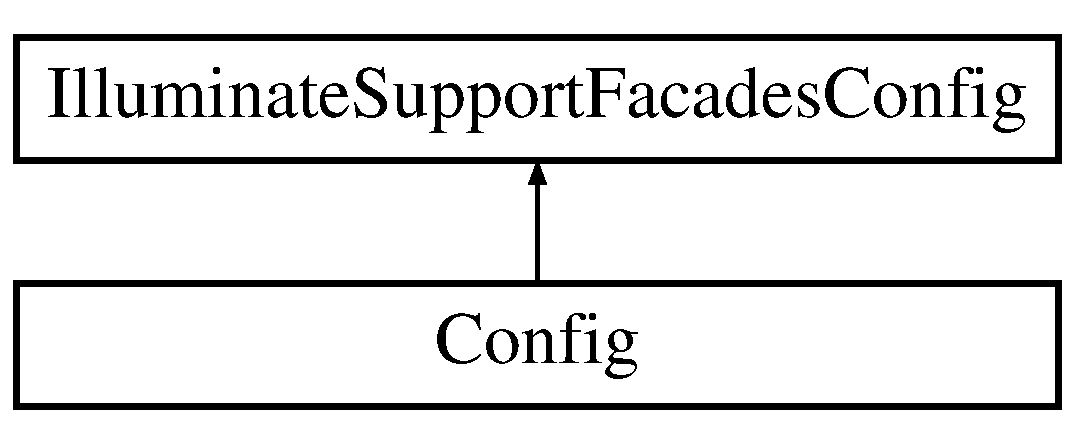
\includegraphics[height=2.000000cm]{class_config}
\end{center}
\end{figure}
\subsection*{Additional Inherited Members}


The documentation for this class was generated from the following file\+:\begin{DoxyCompactItemize}
\item 
\+\_\+ide\+\_\+helper.\+php\end{DoxyCompactItemize}

\hypertarget{class_illuminate_1_1_support_1_1_facades_1_1_cookie}{}\section{Illuminate\textbackslash{}Support\textbackslash{}Facades\textbackslash{}Cookie Class Reference}
\label{class_illuminate_1_1_support_1_1_facades_1_1_cookie}\index{Illuminate\textbackslash{}\+Support\textbackslash{}\+Facades\textbackslash{}\+Cookie@{Illuminate\textbackslash{}\+Support\textbackslash{}\+Facades\textbackslash{}\+Cookie}}
Inheritance diagram for Illuminate\textbackslash{}Support\textbackslash{}Facades\textbackslash{}Cookie\+:\begin{figure}[H]
\begin{center}
\leavevmode
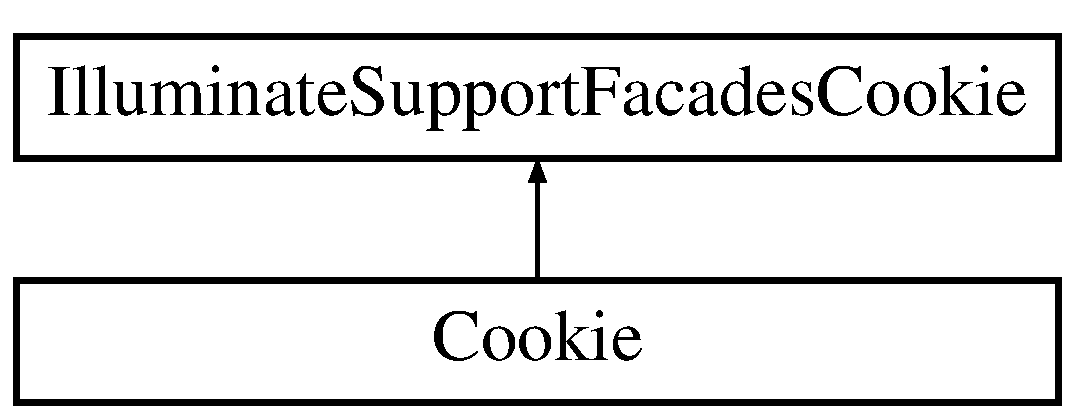
\includegraphics[height=2.000000cm]{class_illuminate_1_1_support_1_1_facades_1_1_cookie}
\end{center}
\end{figure}
\subsection*{Static Public Member Functions}
\begin{DoxyCompactItemize}
\item 
static \mbox{\hyperlink{class_illuminate_1_1_support_1_1_facades_1_1_cookie_afd4e81472bf1dcdc75900bef6a35718d}{make}} (\$name, \$value, \$minutes=0, \$path=null, \$domain=null, \$secure=false, \$http\+Only=true, \$raw=false, \$same\+Site=null)
\item 
static \mbox{\hyperlink{class_illuminate_1_1_support_1_1_facades_1_1_cookie_a8c53563a74ebc6627ff18f490dc188bd}{forever}} (\$name, \$value, \$path=null, \$domain=null, \$secure=false, \$http\+Only=true, \$raw=false, \$same\+Site=null)
\item 
static \mbox{\hyperlink{class_illuminate_1_1_support_1_1_facades_1_1_cookie_a3e7bf07e1e089ddc3588dc686b61207f}{forget}} (\$name, \$path=null, \$domain=null)
\item 
static \mbox{\hyperlink{class_illuminate_1_1_support_1_1_facades_1_1_cookie_a044ed9de6b432c56f78571b56b834f57}{has\+Queued}} (\$key)
\item 
static \mbox{\hyperlink{class_illuminate_1_1_support_1_1_facades_1_1_cookie_a49f771a37e7f2ada5d03c132bef166a3}{queued}} (\$key, \$default=null)
\item 
static \mbox{\hyperlink{class_illuminate_1_1_support_1_1_facades_1_1_cookie_ae325fe7d454cb2e9beb73b3968aeec50}{queue}} (\$parameters=null)
\item 
static \mbox{\hyperlink{class_illuminate_1_1_support_1_1_facades_1_1_cookie_a4a30cd4fe0e78ba8debf5ccd1b543923}{unqueue}} (\$name)
\item 
static \mbox{\hyperlink{class_illuminate_1_1_support_1_1_facades_1_1_cookie_ad50ea75cd9b57428c3945e55a42c154b}{set\+Default\+Path\+And\+Domain}} (\$path, \$domain, \$secure=false, \$same\+Site=null)
\item 
static \mbox{\hyperlink{class_illuminate_1_1_support_1_1_facades_1_1_cookie_ae7de7df09b6a05ed10f9d261d8dda31b}{get\+Queued\+Cookies}} ()
\end{DoxyCompactItemize}


\subsection{Member Function Documentation}
\mbox{\Hypertarget{class_illuminate_1_1_support_1_1_facades_1_1_cookie_a8c53563a74ebc6627ff18f490dc188bd}\label{class_illuminate_1_1_support_1_1_facades_1_1_cookie_a8c53563a74ebc6627ff18f490dc188bd}} 
\index{Illuminate\+::\+Support\+::\+Facades\+::\+Cookie@{Illuminate\+::\+Support\+::\+Facades\+::\+Cookie}!forever@{forever}}
\index{forever@{forever}!Illuminate\+::\+Support\+::\+Facades\+::\+Cookie@{Illuminate\+::\+Support\+::\+Facades\+::\+Cookie}}
\subsubsection{\texorpdfstring{forever()}{forever()}}
{\footnotesize\ttfamily static Illuminate\textbackslash{}\+Support\textbackslash{}\+Facades\textbackslash{}\+Cookie\+::forever (\begin{DoxyParamCaption}\item[{}]{\$name,  }\item[{}]{\$value,  }\item[{}]{\$path = {\ttfamily null},  }\item[{}]{\$domain = {\ttfamily null},  }\item[{}]{\$secure = {\ttfamily false},  }\item[{}]{\$http\+Only = {\ttfamily true},  }\item[{}]{\$raw = {\ttfamily false},  }\item[{}]{\$same\+Site = {\ttfamily null} }\end{DoxyParamCaption})\hspace{0.3cm}{\ttfamily [static]}}

Create a cookie that lasts \char`\"{}forever\char`\"{} (five years).


\begin{DoxyParams}[1]{Parameters}
string & {\em \$name} & \\
\hline
string & {\em \$value} & \\
\hline
string & {\em \$path} & \\
\hline
string & {\em \$domain} & \\
\hline
bool & {\em \$secure} & \\
\hline
bool & {\em \$http\+Only} & \\
\hline
bool & {\em \$raw} & \\
\hline
string | null & {\em \$same\+Site} & \\
\hline
\end{DoxyParams}
\begin{DoxyReturn}{Returns}

\end{DoxyReturn}
\mbox{\Hypertarget{class_illuminate_1_1_support_1_1_facades_1_1_cookie_a3e7bf07e1e089ddc3588dc686b61207f}\label{class_illuminate_1_1_support_1_1_facades_1_1_cookie_a3e7bf07e1e089ddc3588dc686b61207f}} 
\index{Illuminate\+::\+Support\+::\+Facades\+::\+Cookie@{Illuminate\+::\+Support\+::\+Facades\+::\+Cookie}!forget@{forget}}
\index{forget@{forget}!Illuminate\+::\+Support\+::\+Facades\+::\+Cookie@{Illuminate\+::\+Support\+::\+Facades\+::\+Cookie}}
\subsubsection{\texorpdfstring{forget()}{forget()}}
{\footnotesize\ttfamily static Illuminate\textbackslash{}\+Support\textbackslash{}\+Facades\textbackslash{}\+Cookie\+::forget (\begin{DoxyParamCaption}\item[{}]{\$name,  }\item[{}]{\$path = {\ttfamily null},  }\item[{}]{\$domain = {\ttfamily null} }\end{DoxyParamCaption})\hspace{0.3cm}{\ttfamily [static]}}

Expire the given cookie.


\begin{DoxyParams}[1]{Parameters}
string & {\em \$name} & \\
\hline
string & {\em \$path} & \\
\hline
string & {\em \$domain} & \\
\hline
\end{DoxyParams}
\begin{DoxyReturn}{Returns}

\end{DoxyReturn}
\mbox{\Hypertarget{class_illuminate_1_1_support_1_1_facades_1_1_cookie_ae7de7df09b6a05ed10f9d261d8dda31b}\label{class_illuminate_1_1_support_1_1_facades_1_1_cookie_ae7de7df09b6a05ed10f9d261d8dda31b}} 
\index{Illuminate\+::\+Support\+::\+Facades\+::\+Cookie@{Illuminate\+::\+Support\+::\+Facades\+::\+Cookie}!get\+Queued\+Cookies@{get\+Queued\+Cookies}}
\index{get\+Queued\+Cookies@{get\+Queued\+Cookies}!Illuminate\+::\+Support\+::\+Facades\+::\+Cookie@{Illuminate\+::\+Support\+::\+Facades\+::\+Cookie}}
\subsubsection{\texorpdfstring{get\+Queued\+Cookies()}{getQueuedCookies()}}
{\footnotesize\ttfamily static Illuminate\textbackslash{}\+Support\textbackslash{}\+Facades\textbackslash{}\+Cookie\+::get\+Queued\+Cookies (\begin{DoxyParamCaption}{ }\end{DoxyParamCaption})\hspace{0.3cm}{\ttfamily [static]}}

Get the cookies which have been queued for the next request.

\begin{DoxyReturn}{Returns}
array 
\end{DoxyReturn}
\mbox{\Hypertarget{class_illuminate_1_1_support_1_1_facades_1_1_cookie_a044ed9de6b432c56f78571b56b834f57}\label{class_illuminate_1_1_support_1_1_facades_1_1_cookie_a044ed9de6b432c56f78571b56b834f57}} 
\index{Illuminate\+::\+Support\+::\+Facades\+::\+Cookie@{Illuminate\+::\+Support\+::\+Facades\+::\+Cookie}!has\+Queued@{has\+Queued}}
\index{has\+Queued@{has\+Queued}!Illuminate\+::\+Support\+::\+Facades\+::\+Cookie@{Illuminate\+::\+Support\+::\+Facades\+::\+Cookie}}
\subsubsection{\texorpdfstring{has\+Queued()}{hasQueued()}}
{\footnotesize\ttfamily static Illuminate\textbackslash{}\+Support\textbackslash{}\+Facades\textbackslash{}\+Cookie\+::has\+Queued (\begin{DoxyParamCaption}\item[{}]{\$key }\end{DoxyParamCaption})\hspace{0.3cm}{\ttfamily [static]}}

Determine if a cookie has been queued.


\begin{DoxyParams}[1]{Parameters}
string & {\em \$key} & \\
\hline
\end{DoxyParams}
\begin{DoxyReturn}{Returns}
bool 
\end{DoxyReturn}
\mbox{\Hypertarget{class_illuminate_1_1_support_1_1_facades_1_1_cookie_afd4e81472bf1dcdc75900bef6a35718d}\label{class_illuminate_1_1_support_1_1_facades_1_1_cookie_afd4e81472bf1dcdc75900bef6a35718d}} 
\index{Illuminate\+::\+Support\+::\+Facades\+::\+Cookie@{Illuminate\+::\+Support\+::\+Facades\+::\+Cookie}!make@{make}}
\index{make@{make}!Illuminate\+::\+Support\+::\+Facades\+::\+Cookie@{Illuminate\+::\+Support\+::\+Facades\+::\+Cookie}}
\subsubsection{\texorpdfstring{make()}{make()}}
{\footnotesize\ttfamily static Illuminate\textbackslash{}\+Support\textbackslash{}\+Facades\textbackslash{}\+Cookie\+::make (\begin{DoxyParamCaption}\item[{}]{\$name,  }\item[{}]{\$value,  }\item[{}]{\$minutes = {\ttfamily 0},  }\item[{}]{\$path = {\ttfamily null},  }\item[{}]{\$domain = {\ttfamily null},  }\item[{}]{\$secure = {\ttfamily false},  }\item[{}]{\$http\+Only = {\ttfamily true},  }\item[{}]{\$raw = {\ttfamily false},  }\item[{}]{\$same\+Site = {\ttfamily null} }\end{DoxyParamCaption})\hspace{0.3cm}{\ttfamily [static]}}

Create a new cookie instance.


\begin{DoxyParams}[1]{Parameters}
string & {\em \$name} & \\
\hline
string & {\em \$value} & \\
\hline
int & {\em \$minutes} & \\
\hline
string & {\em \$path} & \\
\hline
string & {\em \$domain} & \\
\hline
bool & {\em \$secure} & \\
\hline
bool & {\em \$http\+Only} & \\
\hline
bool & {\em \$raw} & \\
\hline
string | null & {\em \$same\+Site} & \\
\hline
\end{DoxyParams}
\begin{DoxyReturn}{Returns}

\end{DoxyReturn}
\mbox{\Hypertarget{class_illuminate_1_1_support_1_1_facades_1_1_cookie_ae325fe7d454cb2e9beb73b3968aeec50}\label{class_illuminate_1_1_support_1_1_facades_1_1_cookie_ae325fe7d454cb2e9beb73b3968aeec50}} 
\index{Illuminate\+::\+Support\+::\+Facades\+::\+Cookie@{Illuminate\+::\+Support\+::\+Facades\+::\+Cookie}!queue@{queue}}
\index{queue@{queue}!Illuminate\+::\+Support\+::\+Facades\+::\+Cookie@{Illuminate\+::\+Support\+::\+Facades\+::\+Cookie}}
\subsubsection{\texorpdfstring{queue()}{queue()}}
{\footnotesize\ttfamily static Illuminate\textbackslash{}\+Support\textbackslash{}\+Facades\textbackslash{}\+Cookie\+::queue (\begin{DoxyParamCaption}\item[{}]{\$parameters = {\ttfamily null} }\end{DoxyParamCaption})\hspace{0.3cm}{\ttfamily [static]}}

\mbox{\hyperlink{class_illuminate_1_1_support_1_1_facades_1_1_queue}{Queue}} a cookie to send with the next response.


\begin{DoxyParams}[1]{Parameters}
array & {\em \$parameters} & \\
\hline
\end{DoxyParams}
\begin{DoxyReturn}{Returns}
void 
\end{DoxyReturn}
\mbox{\Hypertarget{class_illuminate_1_1_support_1_1_facades_1_1_cookie_a49f771a37e7f2ada5d03c132bef166a3}\label{class_illuminate_1_1_support_1_1_facades_1_1_cookie_a49f771a37e7f2ada5d03c132bef166a3}} 
\index{Illuminate\+::\+Support\+::\+Facades\+::\+Cookie@{Illuminate\+::\+Support\+::\+Facades\+::\+Cookie}!queued@{queued}}
\index{queued@{queued}!Illuminate\+::\+Support\+::\+Facades\+::\+Cookie@{Illuminate\+::\+Support\+::\+Facades\+::\+Cookie}}
\subsubsection{\texorpdfstring{queued()}{queued()}}
{\footnotesize\ttfamily static Illuminate\textbackslash{}\+Support\textbackslash{}\+Facades\textbackslash{}\+Cookie\+::queued (\begin{DoxyParamCaption}\item[{}]{\$key,  }\item[{}]{\$default = {\ttfamily null} }\end{DoxyParamCaption})\hspace{0.3cm}{\ttfamily [static]}}

Get a queued cookie instance.


\begin{DoxyParams}[1]{Parameters}
string & {\em \$key} & \\
\hline
mixed & {\em \$default} & \\
\hline
\end{DoxyParams}
\begin{DoxyReturn}{Returns}

\end{DoxyReturn}
\mbox{\Hypertarget{class_illuminate_1_1_support_1_1_facades_1_1_cookie_ad50ea75cd9b57428c3945e55a42c154b}\label{class_illuminate_1_1_support_1_1_facades_1_1_cookie_ad50ea75cd9b57428c3945e55a42c154b}} 
\index{Illuminate\+::\+Support\+::\+Facades\+::\+Cookie@{Illuminate\+::\+Support\+::\+Facades\+::\+Cookie}!set\+Default\+Path\+And\+Domain@{set\+Default\+Path\+And\+Domain}}
\index{set\+Default\+Path\+And\+Domain@{set\+Default\+Path\+And\+Domain}!Illuminate\+::\+Support\+::\+Facades\+::\+Cookie@{Illuminate\+::\+Support\+::\+Facades\+::\+Cookie}}
\subsubsection{\texorpdfstring{set\+Default\+Path\+And\+Domain()}{setDefaultPathAndDomain()}}
{\footnotesize\ttfamily static Illuminate\textbackslash{}\+Support\textbackslash{}\+Facades\textbackslash{}\+Cookie\+::set\+Default\+Path\+And\+Domain (\begin{DoxyParamCaption}\item[{}]{\$path,  }\item[{}]{\$domain,  }\item[{}]{\$secure = {\ttfamily false},  }\item[{}]{\$same\+Site = {\ttfamily null} }\end{DoxyParamCaption})\hspace{0.3cm}{\ttfamily [static]}}

Set the default path and domain for the jar.


\begin{DoxyParams}[1]{Parameters}
string & {\em \$path} & \\
\hline
string & {\em \$domain} & \\
\hline
bool & {\em \$secure} & \\
\hline
string & {\em \$same\+Site} & \\
\hline
\end{DoxyParams}
\begin{DoxyReturn}{Returns}
\$this 
\end{DoxyReturn}
\mbox{\Hypertarget{class_illuminate_1_1_support_1_1_facades_1_1_cookie_a4a30cd4fe0e78ba8debf5ccd1b543923}\label{class_illuminate_1_1_support_1_1_facades_1_1_cookie_a4a30cd4fe0e78ba8debf5ccd1b543923}} 
\index{Illuminate\+::\+Support\+::\+Facades\+::\+Cookie@{Illuminate\+::\+Support\+::\+Facades\+::\+Cookie}!unqueue@{unqueue}}
\index{unqueue@{unqueue}!Illuminate\+::\+Support\+::\+Facades\+::\+Cookie@{Illuminate\+::\+Support\+::\+Facades\+::\+Cookie}}
\subsubsection{\texorpdfstring{unqueue()}{unqueue()}}
{\footnotesize\ttfamily static Illuminate\textbackslash{}\+Support\textbackslash{}\+Facades\textbackslash{}\+Cookie\+::unqueue (\begin{DoxyParamCaption}\item[{}]{\$name }\end{DoxyParamCaption})\hspace{0.3cm}{\ttfamily [static]}}

Remove a cookie from the queue.


\begin{DoxyParams}[1]{Parameters}
string & {\em \$name} & \\
\hline
\end{DoxyParams}
\begin{DoxyReturn}{Returns}
void 
\end{DoxyReturn}


The documentation for this class was generated from the following file\+:\begin{DoxyCompactItemize}
\item 
\+\_\+ide\+\_\+helper.\+php\end{DoxyCompactItemize}

\hypertarget{class_cookie}{}\section{Cookie Class Reference}
\label{class_cookie}\index{Cookie@{Cookie}}
Inheritance diagram for Cookie\+:\begin{figure}[H]
\begin{center}
\leavevmode
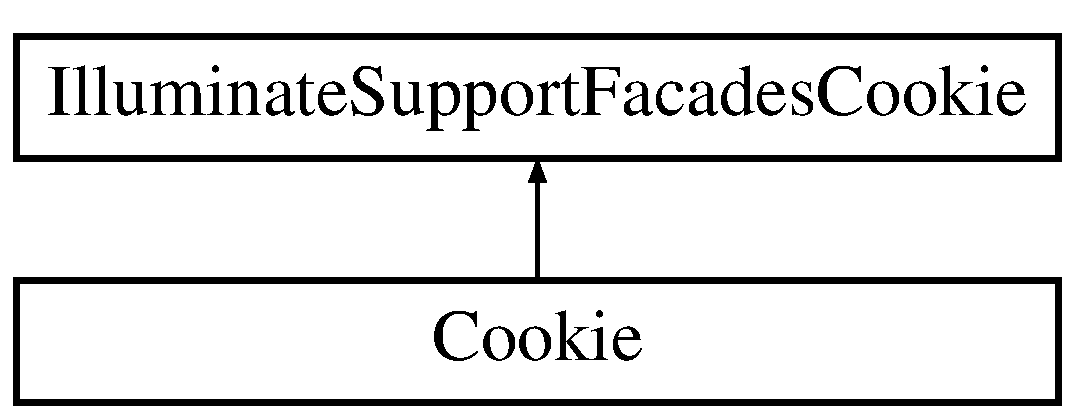
\includegraphics[height=2.000000cm]{class_cookie}
\end{center}
\end{figure}
\subsection*{Additional Inherited Members}


The documentation for this class was generated from the following file\+:\begin{DoxyCompactItemize}
\item 
\+\_\+ide\+\_\+helper.\+php\end{DoxyCompactItemize}

\hypertarget{class_illuminate_1_1_support_1_1_facades_1_1_crypt}{}\section{Illuminate\textbackslash{}Support\textbackslash{}Facades\textbackslash{}Crypt Class Reference}
\label{class_illuminate_1_1_support_1_1_facades_1_1_crypt}\index{Illuminate\textbackslash{}\+Support\textbackslash{}\+Facades\textbackslash{}\+Crypt@{Illuminate\textbackslash{}\+Support\textbackslash{}\+Facades\textbackslash{}\+Crypt}}
Inheritance diagram for Illuminate\textbackslash{}Support\textbackslash{}Facades\textbackslash{}Crypt\+:\begin{figure}[H]
\begin{center}
\leavevmode
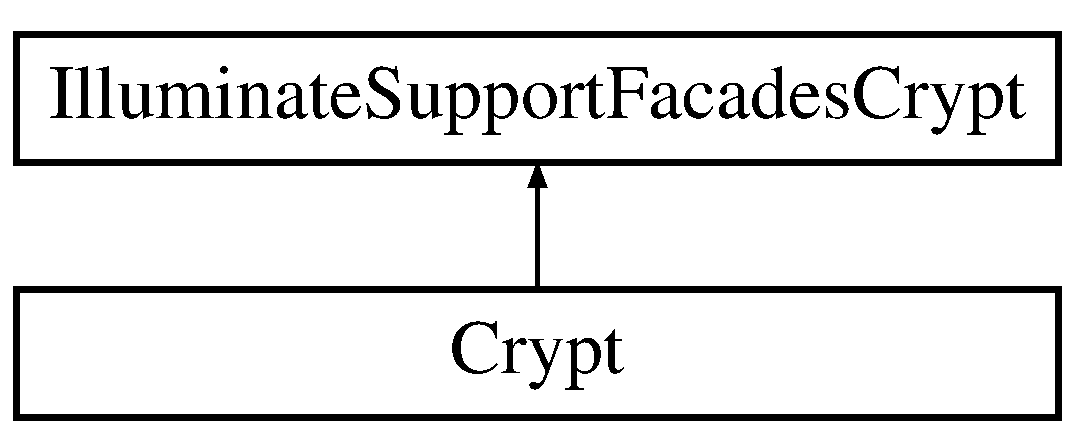
\includegraphics[height=2.000000cm]{class_illuminate_1_1_support_1_1_facades_1_1_crypt}
\end{center}
\end{figure}
\subsection*{Static Public Member Functions}
\begin{DoxyCompactItemize}
\item 
static \mbox{\hyperlink{class_illuminate_1_1_support_1_1_facades_1_1_crypt_a24df7e61205c7f0732b98c430cec2822}{supported}} (\$key, \$cipher)
\item 
static \mbox{\hyperlink{class_illuminate_1_1_support_1_1_facades_1_1_crypt_a3e38bd91ea1c66bd8e37032c98a1ed9f}{generate\+Key}} (\$cipher)
\item 
static \mbox{\hyperlink{class_illuminate_1_1_support_1_1_facades_1_1_crypt_a63be1cb0c27d430f4c01ae6d813239fe}{encrypt}} (\$value, \$serialize=true)
\item 
static \mbox{\hyperlink{class_illuminate_1_1_support_1_1_facades_1_1_crypt_a643aeaa8321cb1813d37cf52b9903714}{encrypt\+String}} (\$value)
\item 
static \mbox{\hyperlink{class_illuminate_1_1_support_1_1_facades_1_1_crypt_a92aa7f25525e25d0c42cc748047b6a00}{decrypt}} (\$payload, \$unserialize=true)
\item 
static \mbox{\hyperlink{class_illuminate_1_1_support_1_1_facades_1_1_crypt_a79cb996624fa47978e78cc48b6f7536d}{decrypt\+String}} (\$payload)
\item 
static \mbox{\hyperlink{class_illuminate_1_1_support_1_1_facades_1_1_crypt_a9067fab9dcf1d9ed7d81439dcaa16a47}{get\+Key}} ()
\end{DoxyCompactItemize}


\subsection{Member Function Documentation}
\mbox{\Hypertarget{class_illuminate_1_1_support_1_1_facades_1_1_crypt_a92aa7f25525e25d0c42cc748047b6a00}\label{class_illuminate_1_1_support_1_1_facades_1_1_crypt_a92aa7f25525e25d0c42cc748047b6a00}} 
\index{Illuminate\+::\+Support\+::\+Facades\+::\+Crypt@{Illuminate\+::\+Support\+::\+Facades\+::\+Crypt}!decrypt@{decrypt}}
\index{decrypt@{decrypt}!Illuminate\+::\+Support\+::\+Facades\+::\+Crypt@{Illuminate\+::\+Support\+::\+Facades\+::\+Crypt}}
\subsubsection{\texorpdfstring{decrypt()}{decrypt()}}
{\footnotesize\ttfamily static Illuminate\textbackslash{}\+Support\textbackslash{}\+Facades\textbackslash{}\+Crypt\+::decrypt (\begin{DoxyParamCaption}\item[{}]{\$payload,  }\item[{}]{\$unserialize = {\ttfamily true} }\end{DoxyParamCaption})\hspace{0.3cm}{\ttfamily [static]}}

Decrypt the given value.


\begin{DoxyParams}[1]{Parameters}
mixed & {\em \$payload} & \\
\hline
bool & {\em \$unserialize} & \\
\hline
\end{DoxyParams}
\begin{DoxyReturn}{Returns}
string 
\end{DoxyReturn}

\begin{DoxyExceptions}{Exceptions}
{\em } & \\
\hline
\end{DoxyExceptions}
\mbox{\Hypertarget{class_illuminate_1_1_support_1_1_facades_1_1_crypt_a79cb996624fa47978e78cc48b6f7536d}\label{class_illuminate_1_1_support_1_1_facades_1_1_crypt_a79cb996624fa47978e78cc48b6f7536d}} 
\index{Illuminate\+::\+Support\+::\+Facades\+::\+Crypt@{Illuminate\+::\+Support\+::\+Facades\+::\+Crypt}!decrypt\+String@{decrypt\+String}}
\index{decrypt\+String@{decrypt\+String}!Illuminate\+::\+Support\+::\+Facades\+::\+Crypt@{Illuminate\+::\+Support\+::\+Facades\+::\+Crypt}}
\subsubsection{\texorpdfstring{decrypt\+String()}{decryptString()}}
{\footnotesize\ttfamily static Illuminate\textbackslash{}\+Support\textbackslash{}\+Facades\textbackslash{}\+Crypt\+::decrypt\+String (\begin{DoxyParamCaption}\item[{}]{\$payload }\end{DoxyParamCaption})\hspace{0.3cm}{\ttfamily [static]}}

Decrypt the given string without unserialization.


\begin{DoxyParams}[1]{Parameters}
string & {\em \$payload} & \\
\hline
\end{DoxyParams}
\begin{DoxyReturn}{Returns}
string 
\end{DoxyReturn}
\mbox{\Hypertarget{class_illuminate_1_1_support_1_1_facades_1_1_crypt_a63be1cb0c27d430f4c01ae6d813239fe}\label{class_illuminate_1_1_support_1_1_facades_1_1_crypt_a63be1cb0c27d430f4c01ae6d813239fe}} 
\index{Illuminate\+::\+Support\+::\+Facades\+::\+Crypt@{Illuminate\+::\+Support\+::\+Facades\+::\+Crypt}!encrypt@{encrypt}}
\index{encrypt@{encrypt}!Illuminate\+::\+Support\+::\+Facades\+::\+Crypt@{Illuminate\+::\+Support\+::\+Facades\+::\+Crypt}}
\subsubsection{\texorpdfstring{encrypt()}{encrypt()}}
{\footnotesize\ttfamily static Illuminate\textbackslash{}\+Support\textbackslash{}\+Facades\textbackslash{}\+Crypt\+::encrypt (\begin{DoxyParamCaption}\item[{}]{\$value,  }\item[{}]{\$serialize = {\ttfamily true} }\end{DoxyParamCaption})\hspace{0.3cm}{\ttfamily [static]}}

Encrypt the given value.


\begin{DoxyParams}[1]{Parameters}
mixed & {\em \$value} & \\
\hline
bool & {\em \$serialize} & \\
\hline
\end{DoxyParams}
\begin{DoxyReturn}{Returns}
string 
\end{DoxyReturn}

\begin{DoxyExceptions}{Exceptions}
{\em } & \\
\hline
\end{DoxyExceptions}
\mbox{\Hypertarget{class_illuminate_1_1_support_1_1_facades_1_1_crypt_a643aeaa8321cb1813d37cf52b9903714}\label{class_illuminate_1_1_support_1_1_facades_1_1_crypt_a643aeaa8321cb1813d37cf52b9903714}} 
\index{Illuminate\+::\+Support\+::\+Facades\+::\+Crypt@{Illuminate\+::\+Support\+::\+Facades\+::\+Crypt}!encrypt\+String@{encrypt\+String}}
\index{encrypt\+String@{encrypt\+String}!Illuminate\+::\+Support\+::\+Facades\+::\+Crypt@{Illuminate\+::\+Support\+::\+Facades\+::\+Crypt}}
\subsubsection{\texorpdfstring{encrypt\+String()}{encryptString()}}
{\footnotesize\ttfamily static Illuminate\textbackslash{}\+Support\textbackslash{}\+Facades\textbackslash{}\+Crypt\+::encrypt\+String (\begin{DoxyParamCaption}\item[{}]{\$value }\end{DoxyParamCaption})\hspace{0.3cm}{\ttfamily [static]}}

Encrypt a string without serialization.


\begin{DoxyParams}[1]{Parameters}
string & {\em \$value} & \\
\hline
\end{DoxyParams}
\begin{DoxyReturn}{Returns}
string 
\end{DoxyReturn}
\mbox{\Hypertarget{class_illuminate_1_1_support_1_1_facades_1_1_crypt_a3e38bd91ea1c66bd8e37032c98a1ed9f}\label{class_illuminate_1_1_support_1_1_facades_1_1_crypt_a3e38bd91ea1c66bd8e37032c98a1ed9f}} 
\index{Illuminate\+::\+Support\+::\+Facades\+::\+Crypt@{Illuminate\+::\+Support\+::\+Facades\+::\+Crypt}!generate\+Key@{generate\+Key}}
\index{generate\+Key@{generate\+Key}!Illuminate\+::\+Support\+::\+Facades\+::\+Crypt@{Illuminate\+::\+Support\+::\+Facades\+::\+Crypt}}
\subsubsection{\texorpdfstring{generate\+Key()}{generateKey()}}
{\footnotesize\ttfamily static Illuminate\textbackslash{}\+Support\textbackslash{}\+Facades\textbackslash{}\+Crypt\+::generate\+Key (\begin{DoxyParamCaption}\item[{}]{\$cipher }\end{DoxyParamCaption})\hspace{0.3cm}{\ttfamily [static]}}

Create a new encryption key for the given cipher.


\begin{DoxyParams}[1]{Parameters}
string & {\em \$cipher} & \\
\hline
\end{DoxyParams}
\begin{DoxyReturn}{Returns}
string 
\end{DoxyReturn}
\mbox{\Hypertarget{class_illuminate_1_1_support_1_1_facades_1_1_crypt_a9067fab9dcf1d9ed7d81439dcaa16a47}\label{class_illuminate_1_1_support_1_1_facades_1_1_crypt_a9067fab9dcf1d9ed7d81439dcaa16a47}} 
\index{Illuminate\+::\+Support\+::\+Facades\+::\+Crypt@{Illuminate\+::\+Support\+::\+Facades\+::\+Crypt}!get\+Key@{get\+Key}}
\index{get\+Key@{get\+Key}!Illuminate\+::\+Support\+::\+Facades\+::\+Crypt@{Illuminate\+::\+Support\+::\+Facades\+::\+Crypt}}
\subsubsection{\texorpdfstring{get\+Key()}{getKey()}}
{\footnotesize\ttfamily static Illuminate\textbackslash{}\+Support\textbackslash{}\+Facades\textbackslash{}\+Crypt\+::get\+Key (\begin{DoxyParamCaption}{ }\end{DoxyParamCaption})\hspace{0.3cm}{\ttfamily [static]}}

Get the encryption key.

\begin{DoxyReturn}{Returns}
string 
\end{DoxyReturn}
\mbox{\Hypertarget{class_illuminate_1_1_support_1_1_facades_1_1_crypt_a24df7e61205c7f0732b98c430cec2822}\label{class_illuminate_1_1_support_1_1_facades_1_1_crypt_a24df7e61205c7f0732b98c430cec2822}} 
\index{Illuminate\+::\+Support\+::\+Facades\+::\+Crypt@{Illuminate\+::\+Support\+::\+Facades\+::\+Crypt}!supported@{supported}}
\index{supported@{supported}!Illuminate\+::\+Support\+::\+Facades\+::\+Crypt@{Illuminate\+::\+Support\+::\+Facades\+::\+Crypt}}
\subsubsection{\texorpdfstring{supported()}{supported()}}
{\footnotesize\ttfamily static Illuminate\textbackslash{}\+Support\textbackslash{}\+Facades\textbackslash{}\+Crypt\+::supported (\begin{DoxyParamCaption}\item[{}]{\$key,  }\item[{}]{\$cipher }\end{DoxyParamCaption})\hspace{0.3cm}{\ttfamily [static]}}

Determine if the given key and cipher combination is valid.


\begin{DoxyParams}[1]{Parameters}
string & {\em \$key} & \\
\hline
string & {\em \$cipher} & \\
\hline
\end{DoxyParams}
\begin{DoxyReturn}{Returns}
bool 
\end{DoxyReturn}


The documentation for this class was generated from the following file\+:\begin{DoxyCompactItemize}
\item 
\+\_\+ide\+\_\+helper.\+php\end{DoxyCompactItemize}

\hypertarget{class_crypt}{}\section{Crypt Class Reference}
\label{class_crypt}\index{Crypt@{Crypt}}
Inheritance diagram for Crypt\+:\begin{figure}[H]
\begin{center}
\leavevmode
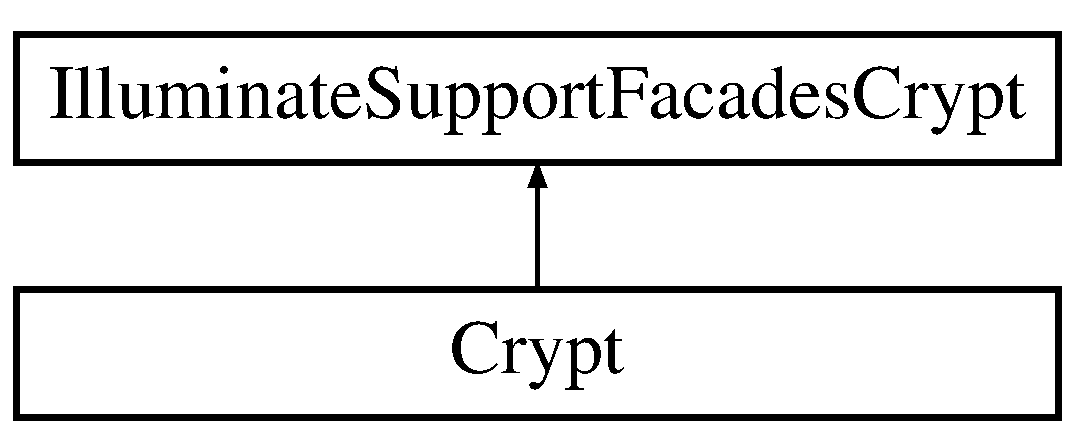
\includegraphics[height=2.000000cm]{class_crypt}
\end{center}
\end{figure}
\subsection*{Additional Inherited Members}


The documentation for this class was generated from the following file\+:\begin{DoxyCompactItemize}
\item 
\+\_\+ide\+\_\+helper.\+php\end{DoxyCompactItemize}

\hypertarget{class_d_b}{}\section{DB Class Reference}
\label{class_d_b}\index{DB@{DB}}
Inheritance diagram for DB\+:\begin{figure}[H]
\begin{center}
\leavevmode
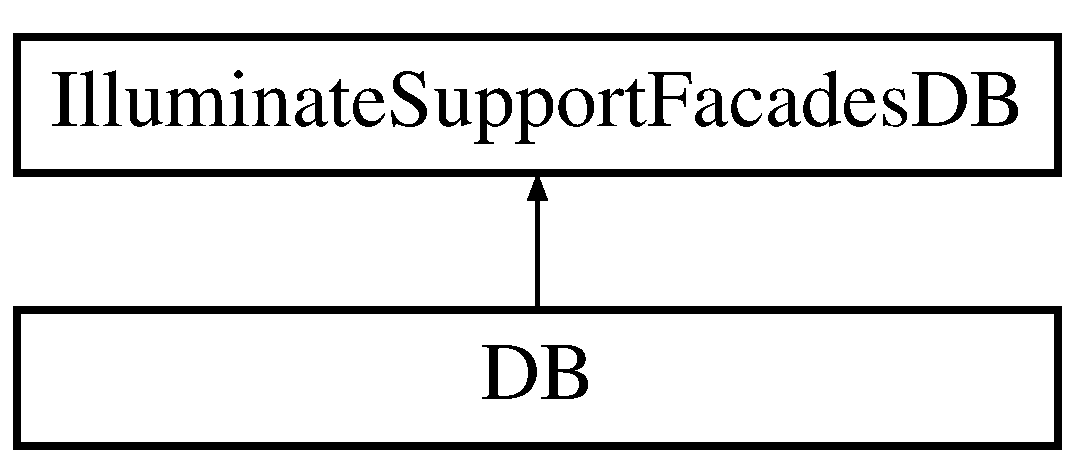
\includegraphics[height=2.000000cm]{class_d_b}
\end{center}
\end{figure}
\subsection*{Additional Inherited Members}


The documentation for this class was generated from the following file\+:\begin{DoxyCompactItemize}
\item 
\+\_\+ide\+\_\+helper.\+php\end{DoxyCompactItemize}

\hypertarget{class_illuminate_1_1_support_1_1_facades_1_1_d_b}{}\section{Illuminate\textbackslash{}Support\textbackslash{}Facades\textbackslash{}DB Class Reference}
\label{class_illuminate_1_1_support_1_1_facades_1_1_d_b}\index{Illuminate\textbackslash{}\+Support\textbackslash{}\+Facades\textbackslash{}\+DB@{Illuminate\textbackslash{}\+Support\textbackslash{}\+Facades\textbackslash{}\+DB}}
Inheritance diagram for Illuminate\textbackslash{}Support\textbackslash{}Facades\textbackslash{}DB\+:\begin{figure}[H]
\begin{center}
\leavevmode
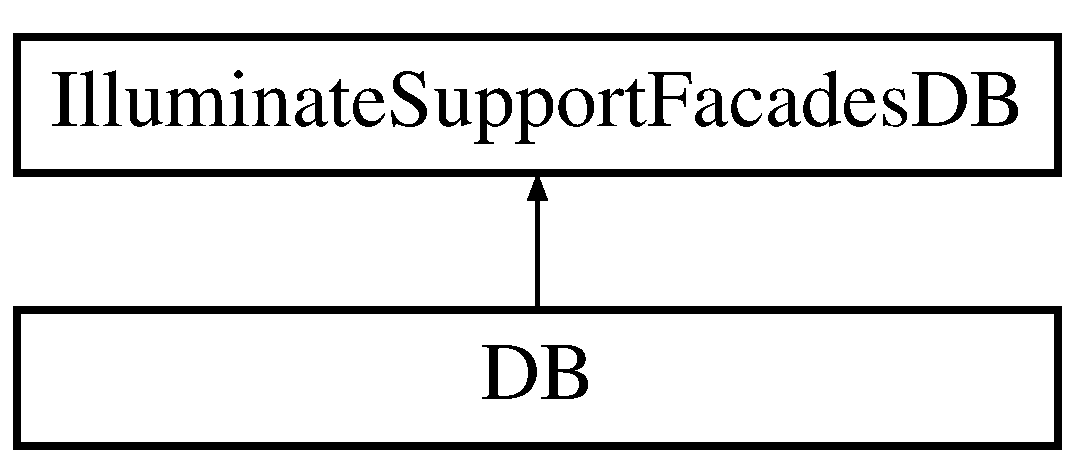
\includegraphics[height=2.000000cm]{class_illuminate_1_1_support_1_1_facades_1_1_d_b}
\end{center}
\end{figure}
\subsection*{Static Public Member Functions}
\begin{DoxyCompactItemize}
\item 
static \mbox{\hyperlink{class_illuminate_1_1_support_1_1_facades_1_1_d_b_af4c07501009e8ba9afb48a1521386349}{connection}} (\$name=null)
\item 
static \mbox{\hyperlink{class_illuminate_1_1_support_1_1_facades_1_1_d_b_ad182e19d6511300709463429b3161e46}{purge}} (\$name=null)
\item 
static \mbox{\hyperlink{class_illuminate_1_1_support_1_1_facades_1_1_d_b_a88b1d08f43661642873618c64b985d1d}{disconnect}} (\$name=null)
\item 
static \mbox{\hyperlink{class_illuminate_1_1_support_1_1_facades_1_1_d_b_a45a46775e77c12f572548c56dd24b596}{reconnect}} (\$name=null)
\item 
static \mbox{\hyperlink{class_illuminate_1_1_support_1_1_facades_1_1_d_b_a9447726af67bae33284f04df631d3ca5}{get\+Default\+Connection}} ()
\item 
static \mbox{\hyperlink{class_illuminate_1_1_support_1_1_facades_1_1_d_b_a99a188fb854611692a62504154ea6a1c}{set\+Default\+Connection}} (\$name)
\item 
static \mbox{\hyperlink{class_illuminate_1_1_support_1_1_facades_1_1_d_b_abcff492f4356880fa4e19317721715a6}{supported\+Drivers}} ()
\item 
static \mbox{\hyperlink{class_illuminate_1_1_support_1_1_facades_1_1_d_b_aa0ab684056ac5ba028a0c66e9a5c05b6}{available\+Drivers}} ()
\item 
static \mbox{\hyperlink{class_illuminate_1_1_support_1_1_facades_1_1_d_b_af20022f9089afcf294af9c0a6929940f}{extend}} (\$name, \$resolver)
\item 
static \mbox{\hyperlink{class_illuminate_1_1_support_1_1_facades_1_1_d_b_ad8ceace824e4fa7e3f0ab8f1af294f10}{get\+Connections}} ()
\item 
static \mbox{\hyperlink{class_illuminate_1_1_support_1_1_facades_1_1_d_b_a8788e832eb3fcb8bb10a7a0a9eaa8580}{get\+Schema\+Builder}} ()
\item 
static \mbox{\hyperlink{class_illuminate_1_1_support_1_1_facades_1_1_d_b_a470a17871255d477ada27e71eb6d0da9}{bind\+Values}} (\$\mbox{\hyperlink{class_illuminate_1_1_support_1_1_facades_1_1_d_b_abe9fe35abfd29aa9bccba94a269c9f25}{statement}}, \$bindings)
\item 
static \mbox{\hyperlink{class_illuminate_1_1_support_1_1_facades_1_1_d_b_a3e64a124726e10a0381bc77b9a0a2323}{use\+Default\+Query\+Grammar}} ()
\item 
static \mbox{\hyperlink{class_illuminate_1_1_support_1_1_facades_1_1_d_b_ae4493947afc8b41bf2e9588c8a3bf1f7}{use\+Default\+Schema\+Grammar}} ()
\item 
static \mbox{\hyperlink{class_illuminate_1_1_support_1_1_facades_1_1_d_b_ab968071b7cebe44a4150e7421be3270d}{use\+Default\+Post\+Processor}} ()
\item 
static \mbox{\hyperlink{class_illuminate_1_1_support_1_1_facades_1_1_d_b_aab727b2bb999e68aafe6ddb5ffb6474a}{table}} (\$table)
\item 
static \mbox{\hyperlink{class_illuminate_1_1_support_1_1_facades_1_1_d_b_ae52c1b74f0ded858ed2dae6342fe5d96}{query}} ()
\item 
static \mbox{\hyperlink{class_illuminate_1_1_support_1_1_facades_1_1_d_b_aba70aca6582e031abf27e5d8fe0a45c7}{select\+One}} (\$\mbox{\hyperlink{class_illuminate_1_1_support_1_1_facades_1_1_d_b_ae52c1b74f0ded858ed2dae6342fe5d96}{query}}, \$bindings=array(), \$use\+Read\+Pdo=true)
\item 
static \mbox{\hyperlink{class_illuminate_1_1_support_1_1_facades_1_1_d_b_aab07a028986590a314f1298b4f111768}{select\+From\+Write\+Connection}} (\$\mbox{\hyperlink{class_illuminate_1_1_support_1_1_facades_1_1_d_b_ae52c1b74f0ded858ed2dae6342fe5d96}{query}}, \$bindings=array())
\item 
static \mbox{\hyperlink{class_illuminate_1_1_support_1_1_facades_1_1_d_b_a5a38160aff9e989f346ceb97d1b765c7}{select}} (\$\mbox{\hyperlink{class_illuminate_1_1_support_1_1_facades_1_1_d_b_ae52c1b74f0ded858ed2dae6342fe5d96}{query}}, \$bindings=array(), \$use\+Read\+Pdo=true)
\item 
static \mbox{\hyperlink{class_illuminate_1_1_support_1_1_facades_1_1_d_b_ab1ad06c52c19e7844542f8bfe41ef765}{cursor}} (\$\mbox{\hyperlink{class_illuminate_1_1_support_1_1_facades_1_1_d_b_ae52c1b74f0ded858ed2dae6342fe5d96}{query}}, \$bindings=array(), \$use\+Read\+Pdo=true)
\item 
static \mbox{\hyperlink{class_illuminate_1_1_support_1_1_facades_1_1_d_b_a3cb47a35deb04e11508027951e732490}{insert}} (\$\mbox{\hyperlink{class_illuminate_1_1_support_1_1_facades_1_1_d_b_ae52c1b74f0ded858ed2dae6342fe5d96}{query}}, \$bindings=array())
\item 
static \mbox{\hyperlink{class_illuminate_1_1_support_1_1_facades_1_1_d_b_a26f6462677e65ac55b2b8b9d59343c9f}{update}} (\$\mbox{\hyperlink{class_illuminate_1_1_support_1_1_facades_1_1_d_b_ae52c1b74f0ded858ed2dae6342fe5d96}{query}}, \$bindings=array())
\item 
static \mbox{\hyperlink{class_illuminate_1_1_support_1_1_facades_1_1_d_b_ae272dffec731836e5186ff97ac416ffa}{delete}} (\$\mbox{\hyperlink{class_illuminate_1_1_support_1_1_facades_1_1_d_b_ae52c1b74f0ded858ed2dae6342fe5d96}{query}}, \$bindings=array())
\item 
static \mbox{\hyperlink{class_illuminate_1_1_support_1_1_facades_1_1_d_b_abe9fe35abfd29aa9bccba94a269c9f25}{statement}} (\$\mbox{\hyperlink{class_illuminate_1_1_support_1_1_facades_1_1_d_b_ae52c1b74f0ded858ed2dae6342fe5d96}{query}}, \$bindings=array())
\item 
static \mbox{\hyperlink{class_illuminate_1_1_support_1_1_facades_1_1_d_b_a1ab200d539f4612e0baf5c935b8f73fe}{affecting\+Statement}} (\$\mbox{\hyperlink{class_illuminate_1_1_support_1_1_facades_1_1_d_b_ae52c1b74f0ded858ed2dae6342fe5d96}{query}}, \$bindings=array())
\item 
static \mbox{\hyperlink{class_illuminate_1_1_support_1_1_facades_1_1_d_b_a2e5507820b20e6d516bcdeb6c48bcc76}{unprepared}} (\$\mbox{\hyperlink{class_illuminate_1_1_support_1_1_facades_1_1_d_b_ae52c1b74f0ded858ed2dae6342fe5d96}{query}})
\item 
static \mbox{\hyperlink{class_illuminate_1_1_support_1_1_facades_1_1_d_b_adf2397397250068e4c6b7e9553963283}{pretend}} (\$callback)
\item 
static \mbox{\hyperlink{class_illuminate_1_1_support_1_1_facades_1_1_d_b_af5ee6d8571a55e7b07c56d40cfd1e131}{prepare\+Bindings}} (\$bindings)
\item 
static \mbox{\hyperlink{class_illuminate_1_1_support_1_1_facades_1_1_d_b_a638ffe152df52b7d57f27545b9b62696}{log\+Query}} (\$\mbox{\hyperlink{class_illuminate_1_1_support_1_1_facades_1_1_d_b_ae52c1b74f0ded858ed2dae6342fe5d96}{query}}, \$bindings, \$time=null)
\item 
static \mbox{\hyperlink{class_illuminate_1_1_support_1_1_facades_1_1_d_b_a8cce2150aaff55e9f96ab589308ef9aa}{listen}} (\$callback)
\item 
static \mbox{\hyperlink{class_illuminate_1_1_support_1_1_facades_1_1_d_b_ac62a351aae4b9c2bcb266ac28304c147}{raw}} (\$value)
\item 
static \mbox{\hyperlink{class_illuminate_1_1_support_1_1_facades_1_1_d_b_a25de82b576ec5d725caa28f2f121393b}{records\+Have\+Been\+Modified}} (\$value=true)
\item 
static \mbox{\hyperlink{class_illuminate_1_1_support_1_1_facades_1_1_d_b_ad3934fcbeb4d850ab6f0f16631d0d64e}{is\+Doctrine\+Available}} ()
\item 
static \mbox{\hyperlink{class_illuminate_1_1_support_1_1_facades_1_1_d_b_adcf6459b45d2f8d7e4dec936776f4a61}{get\+Doctrine\+Column}} (\$\mbox{\hyperlink{class_illuminate_1_1_support_1_1_facades_1_1_d_b_aab727b2bb999e68aafe6ddb5ffb6474a}{table}}, \$column)
\item 
static \mbox{\hyperlink{class_illuminate_1_1_support_1_1_facades_1_1_d_b_ae21d1ea519b88badb605f89d762481f7}{get\+Doctrine\+Schema\+Manager}} ()
\item 
static \mbox{\hyperlink{class_illuminate_1_1_support_1_1_facades_1_1_d_b_a8ffa84e16329112f2d4e846889924f6c}{get\+Doctrine\+Connection}} ()
\item 
static \mbox{\hyperlink{class_illuminate_1_1_support_1_1_facades_1_1_d_b_ad3501e92add7380a83baa4cfdfa7c9ad}{get\+Pdo}} ()
\item 
static \mbox{\hyperlink{class_illuminate_1_1_support_1_1_facades_1_1_d_b_ad1896a49c96025d4adf59acd222e2919}{get\+Read\+Pdo}} ()
\item 
static \mbox{\hyperlink{class_illuminate_1_1_support_1_1_facades_1_1_d_b_a8605551272521c40410a5d88c8cd859c}{set\+Pdo}} (\$pdo)
\item 
static \mbox{\hyperlink{class_illuminate_1_1_support_1_1_facades_1_1_d_b_a2cb0be42acf9aa04a85a4064c4555e95}{set\+Read\+Pdo}} (\$pdo)
\item 
static \mbox{\hyperlink{class_illuminate_1_1_support_1_1_facades_1_1_d_b_ab2c074b6ece85279ce8edbc4279d5c1a}{set\+Reconnector}} (\$reconnector)
\item 
static \mbox{\hyperlink{class_illuminate_1_1_support_1_1_facades_1_1_d_b_a61397bc6e365367fefcf35adf2fb9641}{get\+Name}} ()
\item 
static \mbox{\hyperlink{class_illuminate_1_1_support_1_1_facades_1_1_d_b_a03c2bdae93ae18ffdffe6bc8bd076a12}{get\+Config}} (\$option=null)
\item 
static \mbox{\hyperlink{class_illuminate_1_1_support_1_1_facades_1_1_d_b_a8d8d4afe3eca7fd32e8c4bfb5468fda4}{get\+Driver\+Name}} ()
\item 
static \mbox{\hyperlink{class_illuminate_1_1_support_1_1_facades_1_1_d_b_a82f339b255b77fa638142ccc9b47f155}{get\+Query\+Grammar}} ()
\item 
static \mbox{\hyperlink{class_illuminate_1_1_support_1_1_facades_1_1_d_b_a0ad919b9b783e4aca37c6a10f9c04f6d}{set\+Query\+Grammar}} (\$grammar)
\item 
static \mbox{\hyperlink{class_illuminate_1_1_support_1_1_facades_1_1_d_b_abe52dc2468eb4c844be85421c1363671}{get\+Schema\+Grammar}} ()
\item 
static \mbox{\hyperlink{class_illuminate_1_1_support_1_1_facades_1_1_d_b_ad43cad4300f721b01b177987a20b40ea}{set\+Schema\+Grammar}} (\$grammar)
\item 
static \mbox{\hyperlink{class_illuminate_1_1_support_1_1_facades_1_1_d_b_a0ac3adf5c9525dba15fe714c649ecadc}{get\+Post\+Processor}} ()
\item 
static \mbox{\hyperlink{class_illuminate_1_1_support_1_1_facades_1_1_d_b_a48aba498dabc6974940c6714f14319fa}{set\+Post\+Processor}} (\$processor)
\item 
static \mbox{\hyperlink{class_illuminate_1_1_support_1_1_facades_1_1_d_b_a1ff6d5acb9beaa2bfdcdc13bec293acb}{get\+Event\+Dispatcher}} ()
\item 
static \mbox{\hyperlink{class_illuminate_1_1_support_1_1_facades_1_1_d_b_acebeee92ca49435062d1849ba3486eda}{set\+Event\+Dispatcher}} (\$events)
\item 
static \mbox{\hyperlink{class_illuminate_1_1_support_1_1_facades_1_1_d_b_a5f51e88132ce508656b20d03b8cdd237}{pretending}} ()
\item 
static \mbox{\hyperlink{class_illuminate_1_1_support_1_1_facades_1_1_d_b_a8fc822a5e9a499f19fd9e2d1c4e17bbe}{get\+Query\+Log}} ()
\item 
static \mbox{\hyperlink{class_illuminate_1_1_support_1_1_facades_1_1_d_b_ac14e8afef3256b2eb48f7a6a6b85759c}{flush\+Query\+Log}} ()
\item 
static \mbox{\hyperlink{class_illuminate_1_1_support_1_1_facades_1_1_d_b_a62a569b09967a98988e3e8241e92688a}{enable\+Query\+Log}} ()
\item 
static \mbox{\hyperlink{class_illuminate_1_1_support_1_1_facades_1_1_d_b_a8425946527ebafc412ad410be1db3bc7}{disable\+Query\+Log}} ()
\item 
static \mbox{\hyperlink{class_illuminate_1_1_support_1_1_facades_1_1_d_b_a2457a232d9ccf13ded59a39345635dee}{logging}} ()
\item 
static \mbox{\hyperlink{class_illuminate_1_1_support_1_1_facades_1_1_d_b_a91a05da0ccd778d6b896ec34b2f5f15d}{get\+Database\+Name}} ()
\item 
static \mbox{\hyperlink{class_illuminate_1_1_support_1_1_facades_1_1_d_b_a7fbe4bc4cc8a6fcd8bc87d024dc09cd7}{set\+Database\+Name}} (\$database)
\item 
static \mbox{\hyperlink{class_illuminate_1_1_support_1_1_facades_1_1_d_b_a9aa67ed692d97343d3d1abf5d40fd52b}{get\+Table\+Prefix}} ()
\item 
static \mbox{\hyperlink{class_illuminate_1_1_support_1_1_facades_1_1_d_b_a6eda107e9bd63c513cba9b353d7bfd63}{set\+Table\+Prefix}} (\$prefix)
\item 
static \mbox{\hyperlink{class_illuminate_1_1_support_1_1_facades_1_1_d_b_a6f0a757193d06d182a275d5db6508f5e}{with\+Table\+Prefix}} (\$grammar)
\item 
static \mbox{\hyperlink{class_illuminate_1_1_support_1_1_facades_1_1_d_b_a10db5fb30457d640eea8b068d3012141}{resolver\+For}} (\$driver, \$callback)
\item 
static \mbox{\hyperlink{class_illuminate_1_1_support_1_1_facades_1_1_d_b_a098ac61334abaebf74a0c46ed69eb935}{get\+Resolver}} (\$driver)
\item 
static \mbox{\hyperlink{class_illuminate_1_1_support_1_1_facades_1_1_d_b_a1d5bf5be3c6dcae5917b448f18ff67a6}{transaction}} (\$callback, \$attempts=1)
\item 
static \mbox{\hyperlink{class_illuminate_1_1_support_1_1_facades_1_1_d_b_ae7c00d6d13e51835129058756dc30a6d}{begin\+Transaction}} ()
\item 
static \mbox{\hyperlink{class_illuminate_1_1_support_1_1_facades_1_1_d_b_ab0eda4c9662e5437e6bc14ba068b7a19}{commit}} ()
\item 
static \mbox{\hyperlink{class_illuminate_1_1_support_1_1_facades_1_1_d_b_a34ba448ce0e8c6bf4128756ee3a591fe}{roll\+Back}} (\$to\+Level=null)
\item 
static \mbox{\hyperlink{class_illuminate_1_1_support_1_1_facades_1_1_d_b_a57ef617f66d04d72755eb52f0ec69785}{transaction\+Level}} ()
\end{DoxyCompactItemize}


\subsection{Member Function Documentation}
\mbox{\Hypertarget{class_illuminate_1_1_support_1_1_facades_1_1_d_b_a1ab200d539f4612e0baf5c935b8f73fe}\label{class_illuminate_1_1_support_1_1_facades_1_1_d_b_a1ab200d539f4612e0baf5c935b8f73fe}} 
\index{Illuminate\+::\+Support\+::\+Facades\+::\+DB@{Illuminate\+::\+Support\+::\+Facades\+::\+DB}!affecting\+Statement@{affecting\+Statement}}
\index{affecting\+Statement@{affecting\+Statement}!Illuminate\+::\+Support\+::\+Facades\+::\+DB@{Illuminate\+::\+Support\+::\+Facades\+::\+DB}}
\subsubsection{\texorpdfstring{affecting\+Statement()}{affectingStatement()}}
{\footnotesize\ttfamily static Illuminate\textbackslash{}\+Support\textbackslash{}\+Facades\textbackslash{}\+D\+B\+::affecting\+Statement (\begin{DoxyParamCaption}\item[{}]{\$query,  }\item[{}]{\$bindings = {\ttfamily array()} }\end{DoxyParamCaption})\hspace{0.3cm}{\ttfamily [static]}}

Run an S\+QL statement and get the number of rows affected.


\begin{DoxyParams}[1]{Parameters}
string & {\em \$query} & \\
\hline
array & {\em \$bindings} & \\
\hline
\end{DoxyParams}
\begin{DoxyReturn}{Returns}
int 
\end{DoxyReturn}
\mbox{\Hypertarget{class_illuminate_1_1_support_1_1_facades_1_1_d_b_aa0ab684056ac5ba028a0c66e9a5c05b6}\label{class_illuminate_1_1_support_1_1_facades_1_1_d_b_aa0ab684056ac5ba028a0c66e9a5c05b6}} 
\index{Illuminate\+::\+Support\+::\+Facades\+::\+DB@{Illuminate\+::\+Support\+::\+Facades\+::\+DB}!available\+Drivers@{available\+Drivers}}
\index{available\+Drivers@{available\+Drivers}!Illuminate\+::\+Support\+::\+Facades\+::\+DB@{Illuminate\+::\+Support\+::\+Facades\+::\+DB}}
\subsubsection{\texorpdfstring{available\+Drivers()}{availableDrivers()}}
{\footnotesize\ttfamily static Illuminate\textbackslash{}\+Support\textbackslash{}\+Facades\textbackslash{}\+D\+B\+::available\+Drivers (\begin{DoxyParamCaption}{ }\end{DoxyParamCaption})\hspace{0.3cm}{\ttfamily [static]}}

Get all of the drivers that are actually available.

\begin{DoxyReturn}{Returns}
array 
\end{DoxyReturn}
\mbox{\Hypertarget{class_illuminate_1_1_support_1_1_facades_1_1_d_b_ae7c00d6d13e51835129058756dc30a6d}\label{class_illuminate_1_1_support_1_1_facades_1_1_d_b_ae7c00d6d13e51835129058756dc30a6d}} 
\index{Illuminate\+::\+Support\+::\+Facades\+::\+DB@{Illuminate\+::\+Support\+::\+Facades\+::\+DB}!begin\+Transaction@{begin\+Transaction}}
\index{begin\+Transaction@{begin\+Transaction}!Illuminate\+::\+Support\+::\+Facades\+::\+DB@{Illuminate\+::\+Support\+::\+Facades\+::\+DB}}
\subsubsection{\texorpdfstring{begin\+Transaction()}{beginTransaction()}}
{\footnotesize\ttfamily static Illuminate\textbackslash{}\+Support\textbackslash{}\+Facades\textbackslash{}\+D\+B\+::begin\+Transaction (\begin{DoxyParamCaption}{ }\end{DoxyParamCaption})\hspace{0.3cm}{\ttfamily [static]}}

Start a new database transaction.

\begin{DoxyReturn}{Returns}
void 
\end{DoxyReturn}

\begin{DoxyExceptions}{Exceptions}
{\em } & \\
\hline
\end{DoxyExceptions}
\mbox{\Hypertarget{class_illuminate_1_1_support_1_1_facades_1_1_d_b_a470a17871255d477ada27e71eb6d0da9}\label{class_illuminate_1_1_support_1_1_facades_1_1_d_b_a470a17871255d477ada27e71eb6d0da9}} 
\index{Illuminate\+::\+Support\+::\+Facades\+::\+DB@{Illuminate\+::\+Support\+::\+Facades\+::\+DB}!bind\+Values@{bind\+Values}}
\index{bind\+Values@{bind\+Values}!Illuminate\+::\+Support\+::\+Facades\+::\+DB@{Illuminate\+::\+Support\+::\+Facades\+::\+DB}}
\subsubsection{\texorpdfstring{bind\+Values()}{bindValues()}}
{\footnotesize\ttfamily static Illuminate\textbackslash{}\+Support\textbackslash{}\+Facades\textbackslash{}\+D\+B\+::bind\+Values (\begin{DoxyParamCaption}\item[{}]{\$statement,  }\item[{}]{\$bindings }\end{DoxyParamCaption})\hspace{0.3cm}{\ttfamily [static]}}

Bind values to their parameters in the given statement.


\begin{DoxyParams}[1]{Parameters}
\textbackslash{}\+P\+D\+O\+Statement & {\em \$statement} & \\
\hline
array & {\em \$bindings} & \\
\hline
\end{DoxyParams}
\begin{DoxyReturn}{Returns}
void 
\end{DoxyReturn}
\mbox{\Hypertarget{class_illuminate_1_1_support_1_1_facades_1_1_d_b_ab0eda4c9662e5437e6bc14ba068b7a19}\label{class_illuminate_1_1_support_1_1_facades_1_1_d_b_ab0eda4c9662e5437e6bc14ba068b7a19}} 
\index{Illuminate\+::\+Support\+::\+Facades\+::\+DB@{Illuminate\+::\+Support\+::\+Facades\+::\+DB}!commit@{commit}}
\index{commit@{commit}!Illuminate\+::\+Support\+::\+Facades\+::\+DB@{Illuminate\+::\+Support\+::\+Facades\+::\+DB}}
\subsubsection{\texorpdfstring{commit()}{commit()}}
{\footnotesize\ttfamily static Illuminate\textbackslash{}\+Support\textbackslash{}\+Facades\textbackslash{}\+D\+B\+::commit (\begin{DoxyParamCaption}{ }\end{DoxyParamCaption})\hspace{0.3cm}{\ttfamily [static]}}

Commit the active database transaction.

\begin{DoxyReturn}{Returns}
void 
\end{DoxyReturn}
\mbox{\Hypertarget{class_illuminate_1_1_support_1_1_facades_1_1_d_b_af4c07501009e8ba9afb48a1521386349}\label{class_illuminate_1_1_support_1_1_facades_1_1_d_b_af4c07501009e8ba9afb48a1521386349}} 
\index{Illuminate\+::\+Support\+::\+Facades\+::\+DB@{Illuminate\+::\+Support\+::\+Facades\+::\+DB}!connection@{connection}}
\index{connection@{connection}!Illuminate\+::\+Support\+::\+Facades\+::\+DB@{Illuminate\+::\+Support\+::\+Facades\+::\+DB}}
\subsubsection{\texorpdfstring{connection()}{connection()}}
{\footnotesize\ttfamily static Illuminate\textbackslash{}\+Support\textbackslash{}\+Facades\textbackslash{}\+D\+B\+::connection (\begin{DoxyParamCaption}\item[{}]{\$name = {\ttfamily null} }\end{DoxyParamCaption})\hspace{0.3cm}{\ttfamily [static]}}

Get a database connection instance.


\begin{DoxyParams}[1]{Parameters}
string & {\em \$name} & \\
\hline
\end{DoxyParams}
\begin{DoxyReturn}{Returns}

\end{DoxyReturn}
\mbox{\Hypertarget{class_illuminate_1_1_support_1_1_facades_1_1_d_b_ab1ad06c52c19e7844542f8bfe41ef765}\label{class_illuminate_1_1_support_1_1_facades_1_1_d_b_ab1ad06c52c19e7844542f8bfe41ef765}} 
\index{Illuminate\+::\+Support\+::\+Facades\+::\+DB@{Illuminate\+::\+Support\+::\+Facades\+::\+DB}!cursor@{cursor}}
\index{cursor@{cursor}!Illuminate\+::\+Support\+::\+Facades\+::\+DB@{Illuminate\+::\+Support\+::\+Facades\+::\+DB}}
\subsubsection{\texorpdfstring{cursor()}{cursor()}}
{\footnotesize\ttfamily static Illuminate\textbackslash{}\+Support\textbackslash{}\+Facades\textbackslash{}\+D\+B\+::cursor (\begin{DoxyParamCaption}\item[{}]{\$query,  }\item[{}]{\$bindings = {\ttfamily array()},  }\item[{}]{\$use\+Read\+Pdo = {\ttfamily true} }\end{DoxyParamCaption})\hspace{0.3cm}{\ttfamily [static]}}

Run a select statement against the database and returns a generator.


\begin{DoxyParams}[1]{Parameters}
string & {\em \$query} & \\
\hline
array & {\em \$bindings} & \\
\hline
bool & {\em \$use\+Read\+Pdo} & \\
\hline
\end{DoxyParams}
\begin{DoxyReturn}{Returns}

\end{DoxyReturn}
\mbox{\Hypertarget{class_illuminate_1_1_support_1_1_facades_1_1_d_b_ae272dffec731836e5186ff97ac416ffa}\label{class_illuminate_1_1_support_1_1_facades_1_1_d_b_ae272dffec731836e5186ff97ac416ffa}} 
\index{Illuminate\+::\+Support\+::\+Facades\+::\+DB@{Illuminate\+::\+Support\+::\+Facades\+::\+DB}!delete@{delete}}
\index{delete@{delete}!Illuminate\+::\+Support\+::\+Facades\+::\+DB@{Illuminate\+::\+Support\+::\+Facades\+::\+DB}}
\subsubsection{\texorpdfstring{delete()}{delete()}}
{\footnotesize\ttfamily static Illuminate\textbackslash{}\+Support\textbackslash{}\+Facades\textbackslash{}\+D\+B\+::delete (\begin{DoxyParamCaption}\item[{}]{\$query,  }\item[{}]{\$bindings = {\ttfamily array()} }\end{DoxyParamCaption})\hspace{0.3cm}{\ttfamily [static]}}

Run a delete statement against the database.


\begin{DoxyParams}[1]{Parameters}
string & {\em \$query} & \\
\hline
array & {\em \$bindings} & \\
\hline
\end{DoxyParams}
\begin{DoxyReturn}{Returns}
int 
\end{DoxyReturn}
\mbox{\Hypertarget{class_illuminate_1_1_support_1_1_facades_1_1_d_b_a8425946527ebafc412ad410be1db3bc7}\label{class_illuminate_1_1_support_1_1_facades_1_1_d_b_a8425946527ebafc412ad410be1db3bc7}} 
\index{Illuminate\+::\+Support\+::\+Facades\+::\+DB@{Illuminate\+::\+Support\+::\+Facades\+::\+DB}!disable\+Query\+Log@{disable\+Query\+Log}}
\index{disable\+Query\+Log@{disable\+Query\+Log}!Illuminate\+::\+Support\+::\+Facades\+::\+DB@{Illuminate\+::\+Support\+::\+Facades\+::\+DB}}
\subsubsection{\texorpdfstring{disable\+Query\+Log()}{disableQueryLog()}}
{\footnotesize\ttfamily static Illuminate\textbackslash{}\+Support\textbackslash{}\+Facades\textbackslash{}\+D\+B\+::disable\+Query\+Log (\begin{DoxyParamCaption}{ }\end{DoxyParamCaption})\hspace{0.3cm}{\ttfamily [static]}}

Disable the query log on the connection.

\begin{DoxyReturn}{Returns}
void 
\end{DoxyReturn}
\mbox{\Hypertarget{class_illuminate_1_1_support_1_1_facades_1_1_d_b_a88b1d08f43661642873618c64b985d1d}\label{class_illuminate_1_1_support_1_1_facades_1_1_d_b_a88b1d08f43661642873618c64b985d1d}} 
\index{Illuminate\+::\+Support\+::\+Facades\+::\+DB@{Illuminate\+::\+Support\+::\+Facades\+::\+DB}!disconnect@{disconnect}}
\index{disconnect@{disconnect}!Illuminate\+::\+Support\+::\+Facades\+::\+DB@{Illuminate\+::\+Support\+::\+Facades\+::\+DB}}
\subsubsection{\texorpdfstring{disconnect()}{disconnect()}}
{\footnotesize\ttfamily static Illuminate\textbackslash{}\+Support\textbackslash{}\+Facades\textbackslash{}\+D\+B\+::disconnect (\begin{DoxyParamCaption}\item[{}]{\$name = {\ttfamily null} }\end{DoxyParamCaption})\hspace{0.3cm}{\ttfamily [static]}}

Disconnect from the given database.


\begin{DoxyParams}[1]{Parameters}
string & {\em \$name} & \\
\hline
\end{DoxyParams}
\begin{DoxyReturn}{Returns}
void 
\end{DoxyReturn}
\mbox{\Hypertarget{class_illuminate_1_1_support_1_1_facades_1_1_d_b_a62a569b09967a98988e3e8241e92688a}\label{class_illuminate_1_1_support_1_1_facades_1_1_d_b_a62a569b09967a98988e3e8241e92688a}} 
\index{Illuminate\+::\+Support\+::\+Facades\+::\+DB@{Illuminate\+::\+Support\+::\+Facades\+::\+DB}!enable\+Query\+Log@{enable\+Query\+Log}}
\index{enable\+Query\+Log@{enable\+Query\+Log}!Illuminate\+::\+Support\+::\+Facades\+::\+DB@{Illuminate\+::\+Support\+::\+Facades\+::\+DB}}
\subsubsection{\texorpdfstring{enable\+Query\+Log()}{enableQueryLog()}}
{\footnotesize\ttfamily static Illuminate\textbackslash{}\+Support\textbackslash{}\+Facades\textbackslash{}\+D\+B\+::enable\+Query\+Log (\begin{DoxyParamCaption}{ }\end{DoxyParamCaption})\hspace{0.3cm}{\ttfamily [static]}}

Enable the query log on the connection.

\begin{DoxyReturn}{Returns}
void 
\end{DoxyReturn}
\mbox{\Hypertarget{class_illuminate_1_1_support_1_1_facades_1_1_d_b_af20022f9089afcf294af9c0a6929940f}\label{class_illuminate_1_1_support_1_1_facades_1_1_d_b_af20022f9089afcf294af9c0a6929940f}} 
\index{Illuminate\+::\+Support\+::\+Facades\+::\+DB@{Illuminate\+::\+Support\+::\+Facades\+::\+DB}!extend@{extend}}
\index{extend@{extend}!Illuminate\+::\+Support\+::\+Facades\+::\+DB@{Illuminate\+::\+Support\+::\+Facades\+::\+DB}}
\subsubsection{\texorpdfstring{extend()}{extend()}}
{\footnotesize\ttfamily static Illuminate\textbackslash{}\+Support\textbackslash{}\+Facades\textbackslash{}\+D\+B\+::extend (\begin{DoxyParamCaption}\item[{}]{\$name,  }\item[{}]{\$resolver }\end{DoxyParamCaption})\hspace{0.3cm}{\ttfamily [static]}}

Register an extension connection resolver.


\begin{DoxyParams}[1]{Parameters}
string & {\em \$name} & \\
\hline
callable & {\em \$resolver} & \\
\hline
\end{DoxyParams}
\begin{DoxyReturn}{Returns}
void 
\end{DoxyReturn}
\mbox{\Hypertarget{class_illuminate_1_1_support_1_1_facades_1_1_d_b_ac14e8afef3256b2eb48f7a6a6b85759c}\label{class_illuminate_1_1_support_1_1_facades_1_1_d_b_ac14e8afef3256b2eb48f7a6a6b85759c}} 
\index{Illuminate\+::\+Support\+::\+Facades\+::\+DB@{Illuminate\+::\+Support\+::\+Facades\+::\+DB}!flush\+Query\+Log@{flush\+Query\+Log}}
\index{flush\+Query\+Log@{flush\+Query\+Log}!Illuminate\+::\+Support\+::\+Facades\+::\+DB@{Illuminate\+::\+Support\+::\+Facades\+::\+DB}}
\subsubsection{\texorpdfstring{flush\+Query\+Log()}{flushQueryLog()}}
{\footnotesize\ttfamily static Illuminate\textbackslash{}\+Support\textbackslash{}\+Facades\textbackslash{}\+D\+B\+::flush\+Query\+Log (\begin{DoxyParamCaption}{ }\end{DoxyParamCaption})\hspace{0.3cm}{\ttfamily [static]}}

Clear the query log.

\begin{DoxyReturn}{Returns}
void 
\end{DoxyReturn}
\mbox{\Hypertarget{class_illuminate_1_1_support_1_1_facades_1_1_d_b_a03c2bdae93ae18ffdffe6bc8bd076a12}\label{class_illuminate_1_1_support_1_1_facades_1_1_d_b_a03c2bdae93ae18ffdffe6bc8bd076a12}} 
\index{Illuminate\+::\+Support\+::\+Facades\+::\+DB@{Illuminate\+::\+Support\+::\+Facades\+::\+DB}!get\+Config@{get\+Config}}
\index{get\+Config@{get\+Config}!Illuminate\+::\+Support\+::\+Facades\+::\+DB@{Illuminate\+::\+Support\+::\+Facades\+::\+DB}}
\subsubsection{\texorpdfstring{get\+Config()}{getConfig()}}
{\footnotesize\ttfamily static Illuminate\textbackslash{}\+Support\textbackslash{}\+Facades\textbackslash{}\+D\+B\+::get\+Config (\begin{DoxyParamCaption}\item[{}]{\$option = {\ttfamily null} }\end{DoxyParamCaption})\hspace{0.3cm}{\ttfamily [static]}}

Get an option from the configuration options.


\begin{DoxyParams}[1]{Parameters}
string | null & {\em \$option} & \\
\hline
\end{DoxyParams}
\begin{DoxyReturn}{Returns}
mixed 
\end{DoxyReturn}
\mbox{\Hypertarget{class_illuminate_1_1_support_1_1_facades_1_1_d_b_ad8ceace824e4fa7e3f0ab8f1af294f10}\label{class_illuminate_1_1_support_1_1_facades_1_1_d_b_ad8ceace824e4fa7e3f0ab8f1af294f10}} 
\index{Illuminate\+::\+Support\+::\+Facades\+::\+DB@{Illuminate\+::\+Support\+::\+Facades\+::\+DB}!get\+Connections@{get\+Connections}}
\index{get\+Connections@{get\+Connections}!Illuminate\+::\+Support\+::\+Facades\+::\+DB@{Illuminate\+::\+Support\+::\+Facades\+::\+DB}}
\subsubsection{\texorpdfstring{get\+Connections()}{getConnections()}}
{\footnotesize\ttfamily static Illuminate\textbackslash{}\+Support\textbackslash{}\+Facades\textbackslash{}\+D\+B\+::get\+Connections (\begin{DoxyParamCaption}{ }\end{DoxyParamCaption})\hspace{0.3cm}{\ttfamily [static]}}

Return all of the created connections.

\begin{DoxyReturn}{Returns}
array 
\end{DoxyReturn}
\mbox{\Hypertarget{class_illuminate_1_1_support_1_1_facades_1_1_d_b_a91a05da0ccd778d6b896ec34b2f5f15d}\label{class_illuminate_1_1_support_1_1_facades_1_1_d_b_a91a05da0ccd778d6b896ec34b2f5f15d}} 
\index{Illuminate\+::\+Support\+::\+Facades\+::\+DB@{Illuminate\+::\+Support\+::\+Facades\+::\+DB}!get\+Database\+Name@{get\+Database\+Name}}
\index{get\+Database\+Name@{get\+Database\+Name}!Illuminate\+::\+Support\+::\+Facades\+::\+DB@{Illuminate\+::\+Support\+::\+Facades\+::\+DB}}
\subsubsection{\texorpdfstring{get\+Database\+Name()}{getDatabaseName()}}
{\footnotesize\ttfamily static Illuminate\textbackslash{}\+Support\textbackslash{}\+Facades\textbackslash{}\+D\+B\+::get\+Database\+Name (\begin{DoxyParamCaption}{ }\end{DoxyParamCaption})\hspace{0.3cm}{\ttfamily [static]}}

Get the name of the connected database.

\begin{DoxyReturn}{Returns}
string 
\end{DoxyReturn}
\mbox{\Hypertarget{class_illuminate_1_1_support_1_1_facades_1_1_d_b_a9447726af67bae33284f04df631d3ca5}\label{class_illuminate_1_1_support_1_1_facades_1_1_d_b_a9447726af67bae33284f04df631d3ca5}} 
\index{Illuminate\+::\+Support\+::\+Facades\+::\+DB@{Illuminate\+::\+Support\+::\+Facades\+::\+DB}!get\+Default\+Connection@{get\+Default\+Connection}}
\index{get\+Default\+Connection@{get\+Default\+Connection}!Illuminate\+::\+Support\+::\+Facades\+::\+DB@{Illuminate\+::\+Support\+::\+Facades\+::\+DB}}
\subsubsection{\texorpdfstring{get\+Default\+Connection()}{getDefaultConnection()}}
{\footnotesize\ttfamily static Illuminate\textbackslash{}\+Support\textbackslash{}\+Facades\textbackslash{}\+D\+B\+::get\+Default\+Connection (\begin{DoxyParamCaption}{ }\end{DoxyParamCaption})\hspace{0.3cm}{\ttfamily [static]}}

Get the default connection name.

\begin{DoxyReturn}{Returns}
string 
\end{DoxyReturn}
\mbox{\Hypertarget{class_illuminate_1_1_support_1_1_facades_1_1_d_b_adcf6459b45d2f8d7e4dec936776f4a61}\label{class_illuminate_1_1_support_1_1_facades_1_1_d_b_adcf6459b45d2f8d7e4dec936776f4a61}} 
\index{Illuminate\+::\+Support\+::\+Facades\+::\+DB@{Illuminate\+::\+Support\+::\+Facades\+::\+DB}!get\+Doctrine\+Column@{get\+Doctrine\+Column}}
\index{get\+Doctrine\+Column@{get\+Doctrine\+Column}!Illuminate\+::\+Support\+::\+Facades\+::\+DB@{Illuminate\+::\+Support\+::\+Facades\+::\+DB}}
\subsubsection{\texorpdfstring{get\+Doctrine\+Column()}{getDoctrineColumn()}}
{\footnotesize\ttfamily static Illuminate\textbackslash{}\+Support\textbackslash{}\+Facades\textbackslash{}\+D\+B\+::get\+Doctrine\+Column (\begin{DoxyParamCaption}\item[{}]{\$table,  }\item[{}]{\$column }\end{DoxyParamCaption})\hspace{0.3cm}{\ttfamily [static]}}

Get a Doctrine \mbox{\hyperlink{class_illuminate_1_1_support_1_1_facades_1_1_schema}{Schema}} Column instance.


\begin{DoxyParams}[1]{Parameters}
string & {\em \$table} & \\
\hline
string & {\em \$column} & \\
\hline
\end{DoxyParams}
\begin{DoxyReturn}{Returns}

\end{DoxyReturn}
\mbox{\Hypertarget{class_illuminate_1_1_support_1_1_facades_1_1_d_b_a8ffa84e16329112f2d4e846889924f6c}\label{class_illuminate_1_1_support_1_1_facades_1_1_d_b_a8ffa84e16329112f2d4e846889924f6c}} 
\index{Illuminate\+::\+Support\+::\+Facades\+::\+DB@{Illuminate\+::\+Support\+::\+Facades\+::\+DB}!get\+Doctrine\+Connection@{get\+Doctrine\+Connection}}
\index{get\+Doctrine\+Connection@{get\+Doctrine\+Connection}!Illuminate\+::\+Support\+::\+Facades\+::\+DB@{Illuminate\+::\+Support\+::\+Facades\+::\+DB}}
\subsubsection{\texorpdfstring{get\+Doctrine\+Connection()}{getDoctrineConnection()}}
{\footnotesize\ttfamily static Illuminate\textbackslash{}\+Support\textbackslash{}\+Facades\textbackslash{}\+D\+B\+::get\+Doctrine\+Connection (\begin{DoxyParamCaption}{ }\end{DoxyParamCaption})\hspace{0.3cm}{\ttfamily [static]}}

Get the Doctrine D\+B\+AL database connection instance.

\begin{DoxyReturn}{Returns}

\end{DoxyReturn}
\mbox{\Hypertarget{class_illuminate_1_1_support_1_1_facades_1_1_d_b_ae21d1ea519b88badb605f89d762481f7}\label{class_illuminate_1_1_support_1_1_facades_1_1_d_b_ae21d1ea519b88badb605f89d762481f7}} 
\index{Illuminate\+::\+Support\+::\+Facades\+::\+DB@{Illuminate\+::\+Support\+::\+Facades\+::\+DB}!get\+Doctrine\+Schema\+Manager@{get\+Doctrine\+Schema\+Manager}}
\index{get\+Doctrine\+Schema\+Manager@{get\+Doctrine\+Schema\+Manager}!Illuminate\+::\+Support\+::\+Facades\+::\+DB@{Illuminate\+::\+Support\+::\+Facades\+::\+DB}}
\subsubsection{\texorpdfstring{get\+Doctrine\+Schema\+Manager()}{getDoctrineSchemaManager()}}
{\footnotesize\ttfamily static Illuminate\textbackslash{}\+Support\textbackslash{}\+Facades\textbackslash{}\+D\+B\+::get\+Doctrine\+Schema\+Manager (\begin{DoxyParamCaption}{ }\end{DoxyParamCaption})\hspace{0.3cm}{\ttfamily [static]}}

Get the Doctrine D\+B\+AL schema manager for the connection.

\begin{DoxyReturn}{Returns}

\end{DoxyReturn}
\mbox{\Hypertarget{class_illuminate_1_1_support_1_1_facades_1_1_d_b_a8d8d4afe3eca7fd32e8c4bfb5468fda4}\label{class_illuminate_1_1_support_1_1_facades_1_1_d_b_a8d8d4afe3eca7fd32e8c4bfb5468fda4}} 
\index{Illuminate\+::\+Support\+::\+Facades\+::\+DB@{Illuminate\+::\+Support\+::\+Facades\+::\+DB}!get\+Driver\+Name@{get\+Driver\+Name}}
\index{get\+Driver\+Name@{get\+Driver\+Name}!Illuminate\+::\+Support\+::\+Facades\+::\+DB@{Illuminate\+::\+Support\+::\+Facades\+::\+DB}}
\subsubsection{\texorpdfstring{get\+Driver\+Name()}{getDriverName()}}
{\footnotesize\ttfamily static Illuminate\textbackslash{}\+Support\textbackslash{}\+Facades\textbackslash{}\+D\+B\+::get\+Driver\+Name (\begin{DoxyParamCaption}{ }\end{DoxyParamCaption})\hspace{0.3cm}{\ttfamily [static]}}

Get the P\+DO driver name.

\begin{DoxyReturn}{Returns}
string 
\end{DoxyReturn}
\mbox{\Hypertarget{class_illuminate_1_1_support_1_1_facades_1_1_d_b_a1ff6d5acb9beaa2bfdcdc13bec293acb}\label{class_illuminate_1_1_support_1_1_facades_1_1_d_b_a1ff6d5acb9beaa2bfdcdc13bec293acb}} 
\index{Illuminate\+::\+Support\+::\+Facades\+::\+DB@{Illuminate\+::\+Support\+::\+Facades\+::\+DB}!get\+Event\+Dispatcher@{get\+Event\+Dispatcher}}
\index{get\+Event\+Dispatcher@{get\+Event\+Dispatcher}!Illuminate\+::\+Support\+::\+Facades\+::\+DB@{Illuminate\+::\+Support\+::\+Facades\+::\+DB}}
\subsubsection{\texorpdfstring{get\+Event\+Dispatcher()}{getEventDispatcher()}}
{\footnotesize\ttfamily static Illuminate\textbackslash{}\+Support\textbackslash{}\+Facades\textbackslash{}\+D\+B\+::get\+Event\+Dispatcher (\begin{DoxyParamCaption}{ }\end{DoxyParamCaption})\hspace{0.3cm}{\ttfamily [static]}}

Get the event dispatcher used by the connection.

\begin{DoxyReturn}{Returns}

\end{DoxyReturn}
\mbox{\Hypertarget{class_illuminate_1_1_support_1_1_facades_1_1_d_b_a61397bc6e365367fefcf35adf2fb9641}\label{class_illuminate_1_1_support_1_1_facades_1_1_d_b_a61397bc6e365367fefcf35adf2fb9641}} 
\index{Illuminate\+::\+Support\+::\+Facades\+::\+DB@{Illuminate\+::\+Support\+::\+Facades\+::\+DB}!get\+Name@{get\+Name}}
\index{get\+Name@{get\+Name}!Illuminate\+::\+Support\+::\+Facades\+::\+DB@{Illuminate\+::\+Support\+::\+Facades\+::\+DB}}
\subsubsection{\texorpdfstring{get\+Name()}{getName()}}
{\footnotesize\ttfamily static Illuminate\textbackslash{}\+Support\textbackslash{}\+Facades\textbackslash{}\+D\+B\+::get\+Name (\begin{DoxyParamCaption}{ }\end{DoxyParamCaption})\hspace{0.3cm}{\ttfamily [static]}}

Get the database connection name.

\begin{DoxyReturn}{Returns}
string$\vert$null 
\end{DoxyReturn}
\mbox{\Hypertarget{class_illuminate_1_1_support_1_1_facades_1_1_d_b_ad3501e92add7380a83baa4cfdfa7c9ad}\label{class_illuminate_1_1_support_1_1_facades_1_1_d_b_ad3501e92add7380a83baa4cfdfa7c9ad}} 
\index{Illuminate\+::\+Support\+::\+Facades\+::\+DB@{Illuminate\+::\+Support\+::\+Facades\+::\+DB}!get\+Pdo@{get\+Pdo}}
\index{get\+Pdo@{get\+Pdo}!Illuminate\+::\+Support\+::\+Facades\+::\+DB@{Illuminate\+::\+Support\+::\+Facades\+::\+DB}}
\subsubsection{\texorpdfstring{get\+Pdo()}{getPdo()}}
{\footnotesize\ttfamily static Illuminate\textbackslash{}\+Support\textbackslash{}\+Facades\textbackslash{}\+D\+B\+::get\+Pdo (\begin{DoxyParamCaption}{ }\end{DoxyParamCaption})\hspace{0.3cm}{\ttfamily [static]}}

Get the current P\+DO connection.

\begin{DoxyReturn}{Returns}

\end{DoxyReturn}
\mbox{\Hypertarget{class_illuminate_1_1_support_1_1_facades_1_1_d_b_a0ac3adf5c9525dba15fe714c649ecadc}\label{class_illuminate_1_1_support_1_1_facades_1_1_d_b_a0ac3adf5c9525dba15fe714c649ecadc}} 
\index{Illuminate\+::\+Support\+::\+Facades\+::\+DB@{Illuminate\+::\+Support\+::\+Facades\+::\+DB}!get\+Post\+Processor@{get\+Post\+Processor}}
\index{get\+Post\+Processor@{get\+Post\+Processor}!Illuminate\+::\+Support\+::\+Facades\+::\+DB@{Illuminate\+::\+Support\+::\+Facades\+::\+DB}}
\subsubsection{\texorpdfstring{get\+Post\+Processor()}{getPostProcessor()}}
{\footnotesize\ttfamily static Illuminate\textbackslash{}\+Support\textbackslash{}\+Facades\textbackslash{}\+D\+B\+::get\+Post\+Processor (\begin{DoxyParamCaption}{ }\end{DoxyParamCaption})\hspace{0.3cm}{\ttfamily [static]}}

Get the query post processor used by the connection.

\begin{DoxyReturn}{Returns}

\end{DoxyReturn}
\mbox{\Hypertarget{class_illuminate_1_1_support_1_1_facades_1_1_d_b_a82f339b255b77fa638142ccc9b47f155}\label{class_illuminate_1_1_support_1_1_facades_1_1_d_b_a82f339b255b77fa638142ccc9b47f155}} 
\index{Illuminate\+::\+Support\+::\+Facades\+::\+DB@{Illuminate\+::\+Support\+::\+Facades\+::\+DB}!get\+Query\+Grammar@{get\+Query\+Grammar}}
\index{get\+Query\+Grammar@{get\+Query\+Grammar}!Illuminate\+::\+Support\+::\+Facades\+::\+DB@{Illuminate\+::\+Support\+::\+Facades\+::\+DB}}
\subsubsection{\texorpdfstring{get\+Query\+Grammar()}{getQueryGrammar()}}
{\footnotesize\ttfamily static Illuminate\textbackslash{}\+Support\textbackslash{}\+Facades\textbackslash{}\+D\+B\+::get\+Query\+Grammar (\begin{DoxyParamCaption}{ }\end{DoxyParamCaption})\hspace{0.3cm}{\ttfamily [static]}}

Get the query grammar used by the connection.

\begin{DoxyReturn}{Returns}

\end{DoxyReturn}
\mbox{\Hypertarget{class_illuminate_1_1_support_1_1_facades_1_1_d_b_a8fc822a5e9a499f19fd9e2d1c4e17bbe}\label{class_illuminate_1_1_support_1_1_facades_1_1_d_b_a8fc822a5e9a499f19fd9e2d1c4e17bbe}} 
\index{Illuminate\+::\+Support\+::\+Facades\+::\+DB@{Illuminate\+::\+Support\+::\+Facades\+::\+DB}!get\+Query\+Log@{get\+Query\+Log}}
\index{get\+Query\+Log@{get\+Query\+Log}!Illuminate\+::\+Support\+::\+Facades\+::\+DB@{Illuminate\+::\+Support\+::\+Facades\+::\+DB}}
\subsubsection{\texorpdfstring{get\+Query\+Log()}{getQueryLog()}}
{\footnotesize\ttfamily static Illuminate\textbackslash{}\+Support\textbackslash{}\+Facades\textbackslash{}\+D\+B\+::get\+Query\+Log (\begin{DoxyParamCaption}{ }\end{DoxyParamCaption})\hspace{0.3cm}{\ttfamily [static]}}

Get the connection query log.

\begin{DoxyReturn}{Returns}
array 
\end{DoxyReturn}
\mbox{\Hypertarget{class_illuminate_1_1_support_1_1_facades_1_1_d_b_ad1896a49c96025d4adf59acd222e2919}\label{class_illuminate_1_1_support_1_1_facades_1_1_d_b_ad1896a49c96025d4adf59acd222e2919}} 
\index{Illuminate\+::\+Support\+::\+Facades\+::\+DB@{Illuminate\+::\+Support\+::\+Facades\+::\+DB}!get\+Read\+Pdo@{get\+Read\+Pdo}}
\index{get\+Read\+Pdo@{get\+Read\+Pdo}!Illuminate\+::\+Support\+::\+Facades\+::\+DB@{Illuminate\+::\+Support\+::\+Facades\+::\+DB}}
\subsubsection{\texorpdfstring{get\+Read\+Pdo()}{getReadPdo()}}
{\footnotesize\ttfamily static Illuminate\textbackslash{}\+Support\textbackslash{}\+Facades\textbackslash{}\+D\+B\+::get\+Read\+Pdo (\begin{DoxyParamCaption}{ }\end{DoxyParamCaption})\hspace{0.3cm}{\ttfamily [static]}}

Get the current P\+DO connection used for reading.

\begin{DoxyReturn}{Returns}

\end{DoxyReturn}
\mbox{\Hypertarget{class_illuminate_1_1_support_1_1_facades_1_1_d_b_a098ac61334abaebf74a0c46ed69eb935}\label{class_illuminate_1_1_support_1_1_facades_1_1_d_b_a098ac61334abaebf74a0c46ed69eb935}} 
\index{Illuminate\+::\+Support\+::\+Facades\+::\+DB@{Illuminate\+::\+Support\+::\+Facades\+::\+DB}!get\+Resolver@{get\+Resolver}}
\index{get\+Resolver@{get\+Resolver}!Illuminate\+::\+Support\+::\+Facades\+::\+DB@{Illuminate\+::\+Support\+::\+Facades\+::\+DB}}
\subsubsection{\texorpdfstring{get\+Resolver()}{getResolver()}}
{\footnotesize\ttfamily static Illuminate\textbackslash{}\+Support\textbackslash{}\+Facades\textbackslash{}\+D\+B\+::get\+Resolver (\begin{DoxyParamCaption}\item[{}]{\$driver }\end{DoxyParamCaption})\hspace{0.3cm}{\ttfamily [static]}}

Get the connection resolver for the given driver.


\begin{DoxyParams}[1]{Parameters}
string & {\em \$driver} & \\
\hline
\end{DoxyParams}
\begin{DoxyReturn}{Returns}
mixed 
\end{DoxyReturn}
\mbox{\Hypertarget{class_illuminate_1_1_support_1_1_facades_1_1_d_b_a8788e832eb3fcb8bb10a7a0a9eaa8580}\label{class_illuminate_1_1_support_1_1_facades_1_1_d_b_a8788e832eb3fcb8bb10a7a0a9eaa8580}} 
\index{Illuminate\+::\+Support\+::\+Facades\+::\+DB@{Illuminate\+::\+Support\+::\+Facades\+::\+DB}!get\+Schema\+Builder@{get\+Schema\+Builder}}
\index{get\+Schema\+Builder@{get\+Schema\+Builder}!Illuminate\+::\+Support\+::\+Facades\+::\+DB@{Illuminate\+::\+Support\+::\+Facades\+::\+DB}}
\subsubsection{\texorpdfstring{get\+Schema\+Builder()}{getSchemaBuilder()}}
{\footnotesize\ttfamily static Illuminate\textbackslash{}\+Support\textbackslash{}\+Facades\textbackslash{}\+D\+B\+::get\+Schema\+Builder (\begin{DoxyParamCaption}{ }\end{DoxyParamCaption})\hspace{0.3cm}{\ttfamily [static]}}

Get a schema builder instance for the connection.

\begin{DoxyReturn}{Returns}

\end{DoxyReturn}
\mbox{\Hypertarget{class_illuminate_1_1_support_1_1_facades_1_1_d_b_abe52dc2468eb4c844be85421c1363671}\label{class_illuminate_1_1_support_1_1_facades_1_1_d_b_abe52dc2468eb4c844be85421c1363671}} 
\index{Illuminate\+::\+Support\+::\+Facades\+::\+DB@{Illuminate\+::\+Support\+::\+Facades\+::\+DB}!get\+Schema\+Grammar@{get\+Schema\+Grammar}}
\index{get\+Schema\+Grammar@{get\+Schema\+Grammar}!Illuminate\+::\+Support\+::\+Facades\+::\+DB@{Illuminate\+::\+Support\+::\+Facades\+::\+DB}}
\subsubsection{\texorpdfstring{get\+Schema\+Grammar()}{getSchemaGrammar()}}
{\footnotesize\ttfamily static Illuminate\textbackslash{}\+Support\textbackslash{}\+Facades\textbackslash{}\+D\+B\+::get\+Schema\+Grammar (\begin{DoxyParamCaption}{ }\end{DoxyParamCaption})\hspace{0.3cm}{\ttfamily [static]}}

Get the schema grammar used by the connection.

\begin{DoxyReturn}{Returns}

\end{DoxyReturn}
\mbox{\Hypertarget{class_illuminate_1_1_support_1_1_facades_1_1_d_b_a9aa67ed692d97343d3d1abf5d40fd52b}\label{class_illuminate_1_1_support_1_1_facades_1_1_d_b_a9aa67ed692d97343d3d1abf5d40fd52b}} 
\index{Illuminate\+::\+Support\+::\+Facades\+::\+DB@{Illuminate\+::\+Support\+::\+Facades\+::\+DB}!get\+Table\+Prefix@{get\+Table\+Prefix}}
\index{get\+Table\+Prefix@{get\+Table\+Prefix}!Illuminate\+::\+Support\+::\+Facades\+::\+DB@{Illuminate\+::\+Support\+::\+Facades\+::\+DB}}
\subsubsection{\texorpdfstring{get\+Table\+Prefix()}{getTablePrefix()}}
{\footnotesize\ttfamily static Illuminate\textbackslash{}\+Support\textbackslash{}\+Facades\textbackslash{}\+D\+B\+::get\+Table\+Prefix (\begin{DoxyParamCaption}{ }\end{DoxyParamCaption})\hspace{0.3cm}{\ttfamily [static]}}

Get the table prefix for the connection.

\begin{DoxyReturn}{Returns}
string 
\end{DoxyReturn}
\mbox{\Hypertarget{class_illuminate_1_1_support_1_1_facades_1_1_d_b_a3cb47a35deb04e11508027951e732490}\label{class_illuminate_1_1_support_1_1_facades_1_1_d_b_a3cb47a35deb04e11508027951e732490}} 
\index{Illuminate\+::\+Support\+::\+Facades\+::\+DB@{Illuminate\+::\+Support\+::\+Facades\+::\+DB}!insert@{insert}}
\index{insert@{insert}!Illuminate\+::\+Support\+::\+Facades\+::\+DB@{Illuminate\+::\+Support\+::\+Facades\+::\+DB}}
\subsubsection{\texorpdfstring{insert()}{insert()}}
{\footnotesize\ttfamily static Illuminate\textbackslash{}\+Support\textbackslash{}\+Facades\textbackslash{}\+D\+B\+::insert (\begin{DoxyParamCaption}\item[{}]{\$query,  }\item[{}]{\$bindings = {\ttfamily array()} }\end{DoxyParamCaption})\hspace{0.3cm}{\ttfamily [static]}}

Run an insert statement against the database.


\begin{DoxyParams}[1]{Parameters}
string & {\em \$query} & \\
\hline
array & {\em \$bindings} & \\
\hline
\end{DoxyParams}
\begin{DoxyReturn}{Returns}
bool 
\end{DoxyReturn}
\mbox{\Hypertarget{class_illuminate_1_1_support_1_1_facades_1_1_d_b_ad3934fcbeb4d850ab6f0f16631d0d64e}\label{class_illuminate_1_1_support_1_1_facades_1_1_d_b_ad3934fcbeb4d850ab6f0f16631d0d64e}} 
\index{Illuminate\+::\+Support\+::\+Facades\+::\+DB@{Illuminate\+::\+Support\+::\+Facades\+::\+DB}!is\+Doctrine\+Available@{is\+Doctrine\+Available}}
\index{is\+Doctrine\+Available@{is\+Doctrine\+Available}!Illuminate\+::\+Support\+::\+Facades\+::\+DB@{Illuminate\+::\+Support\+::\+Facades\+::\+DB}}
\subsubsection{\texorpdfstring{is\+Doctrine\+Available()}{isDoctrineAvailable()}}
{\footnotesize\ttfamily static Illuminate\textbackslash{}\+Support\textbackslash{}\+Facades\textbackslash{}\+D\+B\+::is\+Doctrine\+Available (\begin{DoxyParamCaption}{ }\end{DoxyParamCaption})\hspace{0.3cm}{\ttfamily [static]}}

Is Doctrine available?

\begin{DoxyReturn}{Returns}
bool 
\end{DoxyReturn}
\mbox{\Hypertarget{class_illuminate_1_1_support_1_1_facades_1_1_d_b_a8cce2150aaff55e9f96ab589308ef9aa}\label{class_illuminate_1_1_support_1_1_facades_1_1_d_b_a8cce2150aaff55e9f96ab589308ef9aa}} 
\index{Illuminate\+::\+Support\+::\+Facades\+::\+DB@{Illuminate\+::\+Support\+::\+Facades\+::\+DB}!listen@{listen}}
\index{listen@{listen}!Illuminate\+::\+Support\+::\+Facades\+::\+DB@{Illuminate\+::\+Support\+::\+Facades\+::\+DB}}
\subsubsection{\texorpdfstring{listen()}{listen()}}
{\footnotesize\ttfamily static Illuminate\textbackslash{}\+Support\textbackslash{}\+Facades\textbackslash{}\+D\+B\+::listen (\begin{DoxyParamCaption}\item[{}]{\$callback }\end{DoxyParamCaption})\hspace{0.3cm}{\ttfamily [static]}}

Register a database query listener with the connection.


\begin{DoxyParams}[1]{Parameters}
\textbackslash{}\+Closure & {\em \$callback} & \\
\hline
\end{DoxyParams}
\begin{DoxyReturn}{Returns}
void 
\end{DoxyReturn}
\mbox{\Hypertarget{class_illuminate_1_1_support_1_1_facades_1_1_d_b_a2457a232d9ccf13ded59a39345635dee}\label{class_illuminate_1_1_support_1_1_facades_1_1_d_b_a2457a232d9ccf13ded59a39345635dee}} 
\index{Illuminate\+::\+Support\+::\+Facades\+::\+DB@{Illuminate\+::\+Support\+::\+Facades\+::\+DB}!logging@{logging}}
\index{logging@{logging}!Illuminate\+::\+Support\+::\+Facades\+::\+DB@{Illuminate\+::\+Support\+::\+Facades\+::\+DB}}
\subsubsection{\texorpdfstring{logging()}{logging()}}
{\footnotesize\ttfamily static Illuminate\textbackslash{}\+Support\textbackslash{}\+Facades\textbackslash{}\+D\+B\+::logging (\begin{DoxyParamCaption}{ }\end{DoxyParamCaption})\hspace{0.3cm}{\ttfamily [static]}}

Determine whether we\textquotesingle{}re logging queries.

\begin{DoxyReturn}{Returns}
bool 
\end{DoxyReturn}
\mbox{\Hypertarget{class_illuminate_1_1_support_1_1_facades_1_1_d_b_a638ffe152df52b7d57f27545b9b62696}\label{class_illuminate_1_1_support_1_1_facades_1_1_d_b_a638ffe152df52b7d57f27545b9b62696}} 
\index{Illuminate\+::\+Support\+::\+Facades\+::\+DB@{Illuminate\+::\+Support\+::\+Facades\+::\+DB}!log\+Query@{log\+Query}}
\index{log\+Query@{log\+Query}!Illuminate\+::\+Support\+::\+Facades\+::\+DB@{Illuminate\+::\+Support\+::\+Facades\+::\+DB}}
\subsubsection{\texorpdfstring{log\+Query()}{logQuery()}}
{\footnotesize\ttfamily static Illuminate\textbackslash{}\+Support\textbackslash{}\+Facades\textbackslash{}\+D\+B\+::log\+Query (\begin{DoxyParamCaption}\item[{}]{\$query,  }\item[{}]{\$bindings,  }\item[{}]{\$time = {\ttfamily null} }\end{DoxyParamCaption})\hspace{0.3cm}{\ttfamily [static]}}

\mbox{\hyperlink{class_illuminate_1_1_support_1_1_facades_1_1_log}{Log}} a query in the connection\textquotesingle{}s query log.


\begin{DoxyParams}[1]{Parameters}
string & {\em \$query} & \\
\hline
array & {\em \$bindings} & \\
\hline
float | null & {\em \$time} & \\
\hline
\end{DoxyParams}
\begin{DoxyReturn}{Returns}
void 
\end{DoxyReturn}
\mbox{\Hypertarget{class_illuminate_1_1_support_1_1_facades_1_1_d_b_af5ee6d8571a55e7b07c56d40cfd1e131}\label{class_illuminate_1_1_support_1_1_facades_1_1_d_b_af5ee6d8571a55e7b07c56d40cfd1e131}} 
\index{Illuminate\+::\+Support\+::\+Facades\+::\+DB@{Illuminate\+::\+Support\+::\+Facades\+::\+DB}!prepare\+Bindings@{prepare\+Bindings}}
\index{prepare\+Bindings@{prepare\+Bindings}!Illuminate\+::\+Support\+::\+Facades\+::\+DB@{Illuminate\+::\+Support\+::\+Facades\+::\+DB}}
\subsubsection{\texorpdfstring{prepare\+Bindings()}{prepareBindings()}}
{\footnotesize\ttfamily static Illuminate\textbackslash{}\+Support\textbackslash{}\+Facades\textbackslash{}\+D\+B\+::prepare\+Bindings (\begin{DoxyParamCaption}\item[{}]{\$bindings }\end{DoxyParamCaption})\hspace{0.3cm}{\ttfamily [static]}}

Prepare the query bindings for execution.


\begin{DoxyParams}[1]{Parameters}
array & {\em \$bindings} & \\
\hline
\end{DoxyParams}
\begin{DoxyReturn}{Returns}
array 
\end{DoxyReturn}
\mbox{\Hypertarget{class_illuminate_1_1_support_1_1_facades_1_1_d_b_adf2397397250068e4c6b7e9553963283}\label{class_illuminate_1_1_support_1_1_facades_1_1_d_b_adf2397397250068e4c6b7e9553963283}} 
\index{Illuminate\+::\+Support\+::\+Facades\+::\+DB@{Illuminate\+::\+Support\+::\+Facades\+::\+DB}!pretend@{pretend}}
\index{pretend@{pretend}!Illuminate\+::\+Support\+::\+Facades\+::\+DB@{Illuminate\+::\+Support\+::\+Facades\+::\+DB}}
\subsubsection{\texorpdfstring{pretend()}{pretend()}}
{\footnotesize\ttfamily static Illuminate\textbackslash{}\+Support\textbackslash{}\+Facades\textbackslash{}\+D\+B\+::pretend (\begin{DoxyParamCaption}\item[{}]{\$callback }\end{DoxyParamCaption})\hspace{0.3cm}{\ttfamily [static]}}

Execute the given callback in \char`\"{}dry run\char`\"{} mode.


\begin{DoxyParams}[1]{Parameters}
\textbackslash{}\+Closure & {\em \$callback} & \\
\hline
\end{DoxyParams}
\begin{DoxyReturn}{Returns}
array 
\end{DoxyReturn}
\mbox{\Hypertarget{class_illuminate_1_1_support_1_1_facades_1_1_d_b_a5f51e88132ce508656b20d03b8cdd237}\label{class_illuminate_1_1_support_1_1_facades_1_1_d_b_a5f51e88132ce508656b20d03b8cdd237}} 
\index{Illuminate\+::\+Support\+::\+Facades\+::\+DB@{Illuminate\+::\+Support\+::\+Facades\+::\+DB}!pretending@{pretending}}
\index{pretending@{pretending}!Illuminate\+::\+Support\+::\+Facades\+::\+DB@{Illuminate\+::\+Support\+::\+Facades\+::\+DB}}
\subsubsection{\texorpdfstring{pretending()}{pretending()}}
{\footnotesize\ttfamily static Illuminate\textbackslash{}\+Support\textbackslash{}\+Facades\textbackslash{}\+D\+B\+::pretending (\begin{DoxyParamCaption}{ }\end{DoxyParamCaption})\hspace{0.3cm}{\ttfamily [static]}}

Determine if the connection in a \char`\"{}dry run\char`\"{}.

\begin{DoxyReturn}{Returns}
bool 
\end{DoxyReturn}
\mbox{\Hypertarget{class_illuminate_1_1_support_1_1_facades_1_1_d_b_ad182e19d6511300709463429b3161e46}\label{class_illuminate_1_1_support_1_1_facades_1_1_d_b_ad182e19d6511300709463429b3161e46}} 
\index{Illuminate\+::\+Support\+::\+Facades\+::\+DB@{Illuminate\+::\+Support\+::\+Facades\+::\+DB}!purge@{purge}}
\index{purge@{purge}!Illuminate\+::\+Support\+::\+Facades\+::\+DB@{Illuminate\+::\+Support\+::\+Facades\+::\+DB}}
\subsubsection{\texorpdfstring{purge()}{purge()}}
{\footnotesize\ttfamily static Illuminate\textbackslash{}\+Support\textbackslash{}\+Facades\textbackslash{}\+D\+B\+::purge (\begin{DoxyParamCaption}\item[{}]{\$name = {\ttfamily null} }\end{DoxyParamCaption})\hspace{0.3cm}{\ttfamily [static]}}

Disconnect from the given database and remove from local cache.


\begin{DoxyParams}[1]{Parameters}
string & {\em \$name} & \\
\hline
\end{DoxyParams}
\begin{DoxyReturn}{Returns}
void 
\end{DoxyReturn}
\mbox{\Hypertarget{class_illuminate_1_1_support_1_1_facades_1_1_d_b_ae52c1b74f0ded858ed2dae6342fe5d96}\label{class_illuminate_1_1_support_1_1_facades_1_1_d_b_ae52c1b74f0ded858ed2dae6342fe5d96}} 
\index{Illuminate\+::\+Support\+::\+Facades\+::\+DB@{Illuminate\+::\+Support\+::\+Facades\+::\+DB}!query@{query}}
\index{query@{query}!Illuminate\+::\+Support\+::\+Facades\+::\+DB@{Illuminate\+::\+Support\+::\+Facades\+::\+DB}}
\subsubsection{\texorpdfstring{query()}{query()}}
{\footnotesize\ttfamily static Illuminate\textbackslash{}\+Support\textbackslash{}\+Facades\textbackslash{}\+D\+B\+::query (\begin{DoxyParamCaption}{ }\end{DoxyParamCaption})\hspace{0.3cm}{\ttfamily [static]}}

Get a new query builder instance.

\begin{DoxyReturn}{Returns}

\end{DoxyReturn}
\mbox{\Hypertarget{class_illuminate_1_1_support_1_1_facades_1_1_d_b_ac62a351aae4b9c2bcb266ac28304c147}\label{class_illuminate_1_1_support_1_1_facades_1_1_d_b_ac62a351aae4b9c2bcb266ac28304c147}} 
\index{Illuminate\+::\+Support\+::\+Facades\+::\+DB@{Illuminate\+::\+Support\+::\+Facades\+::\+DB}!raw@{raw}}
\index{raw@{raw}!Illuminate\+::\+Support\+::\+Facades\+::\+DB@{Illuminate\+::\+Support\+::\+Facades\+::\+DB}}
\subsubsection{\texorpdfstring{raw()}{raw()}}
{\footnotesize\ttfamily static Illuminate\textbackslash{}\+Support\textbackslash{}\+Facades\textbackslash{}\+D\+B\+::raw (\begin{DoxyParamCaption}\item[{}]{\$value }\end{DoxyParamCaption})\hspace{0.3cm}{\ttfamily [static]}}

Get a new raw query expression.


\begin{DoxyParams}[1]{Parameters}
mixed & {\em \$value} & \\
\hline
\end{DoxyParams}
\begin{DoxyReturn}{Returns}

\end{DoxyReturn}
\mbox{\Hypertarget{class_illuminate_1_1_support_1_1_facades_1_1_d_b_a45a46775e77c12f572548c56dd24b596}\label{class_illuminate_1_1_support_1_1_facades_1_1_d_b_a45a46775e77c12f572548c56dd24b596}} 
\index{Illuminate\+::\+Support\+::\+Facades\+::\+DB@{Illuminate\+::\+Support\+::\+Facades\+::\+DB}!reconnect@{reconnect}}
\index{reconnect@{reconnect}!Illuminate\+::\+Support\+::\+Facades\+::\+DB@{Illuminate\+::\+Support\+::\+Facades\+::\+DB}}
\subsubsection{\texorpdfstring{reconnect()}{reconnect()}}
{\footnotesize\ttfamily static Illuminate\textbackslash{}\+Support\textbackslash{}\+Facades\textbackslash{}\+D\+B\+::reconnect (\begin{DoxyParamCaption}\item[{}]{\$name = {\ttfamily null} }\end{DoxyParamCaption})\hspace{0.3cm}{\ttfamily [static]}}

Reconnect to the given database.


\begin{DoxyParams}[1]{Parameters}
string & {\em \$name} & \\
\hline
\end{DoxyParams}
\begin{DoxyReturn}{Returns}

\end{DoxyReturn}
\mbox{\Hypertarget{class_illuminate_1_1_support_1_1_facades_1_1_d_b_a25de82b576ec5d725caa28f2f121393b}\label{class_illuminate_1_1_support_1_1_facades_1_1_d_b_a25de82b576ec5d725caa28f2f121393b}} 
\index{Illuminate\+::\+Support\+::\+Facades\+::\+DB@{Illuminate\+::\+Support\+::\+Facades\+::\+DB}!records\+Have\+Been\+Modified@{records\+Have\+Been\+Modified}}
\index{records\+Have\+Been\+Modified@{records\+Have\+Been\+Modified}!Illuminate\+::\+Support\+::\+Facades\+::\+DB@{Illuminate\+::\+Support\+::\+Facades\+::\+DB}}
\subsubsection{\texorpdfstring{records\+Have\+Been\+Modified()}{recordsHaveBeenModified()}}
{\footnotesize\ttfamily static Illuminate\textbackslash{}\+Support\textbackslash{}\+Facades\textbackslash{}\+D\+B\+::records\+Have\+Been\+Modified (\begin{DoxyParamCaption}\item[{}]{\$value = {\ttfamily true} }\end{DoxyParamCaption})\hspace{0.3cm}{\ttfamily [static]}}

Indicate if any records have been modified.


\begin{DoxyParams}[1]{Parameters}
bool & {\em \$value} & \\
\hline
\end{DoxyParams}
\begin{DoxyReturn}{Returns}
void 
\end{DoxyReturn}
\mbox{\Hypertarget{class_illuminate_1_1_support_1_1_facades_1_1_d_b_a10db5fb30457d640eea8b068d3012141}\label{class_illuminate_1_1_support_1_1_facades_1_1_d_b_a10db5fb30457d640eea8b068d3012141}} 
\index{Illuminate\+::\+Support\+::\+Facades\+::\+DB@{Illuminate\+::\+Support\+::\+Facades\+::\+DB}!resolver\+For@{resolver\+For}}
\index{resolver\+For@{resolver\+For}!Illuminate\+::\+Support\+::\+Facades\+::\+DB@{Illuminate\+::\+Support\+::\+Facades\+::\+DB}}
\subsubsection{\texorpdfstring{resolver\+For()}{resolverFor()}}
{\footnotesize\ttfamily static Illuminate\textbackslash{}\+Support\textbackslash{}\+Facades\textbackslash{}\+D\+B\+::resolver\+For (\begin{DoxyParamCaption}\item[{}]{\$driver,  }\item[{}]{\$callback }\end{DoxyParamCaption})\hspace{0.3cm}{\ttfamily [static]}}

Register a connection resolver.


\begin{DoxyParams}[1]{Parameters}
string & {\em \$driver} & \\
\hline
\textbackslash{}\+Closure & {\em \$callback} & \\
\hline
\end{DoxyParams}
\begin{DoxyReturn}{Returns}
void 
\end{DoxyReturn}
\mbox{\Hypertarget{class_illuminate_1_1_support_1_1_facades_1_1_d_b_a34ba448ce0e8c6bf4128756ee3a591fe}\label{class_illuminate_1_1_support_1_1_facades_1_1_d_b_a34ba448ce0e8c6bf4128756ee3a591fe}} 
\index{Illuminate\+::\+Support\+::\+Facades\+::\+DB@{Illuminate\+::\+Support\+::\+Facades\+::\+DB}!roll\+Back@{roll\+Back}}
\index{roll\+Back@{roll\+Back}!Illuminate\+::\+Support\+::\+Facades\+::\+DB@{Illuminate\+::\+Support\+::\+Facades\+::\+DB}}
\subsubsection{\texorpdfstring{roll\+Back()}{rollBack()}}
{\footnotesize\ttfamily static Illuminate\textbackslash{}\+Support\textbackslash{}\+Facades\textbackslash{}\+D\+B\+::roll\+Back (\begin{DoxyParamCaption}\item[{}]{\$to\+Level = {\ttfamily null} }\end{DoxyParamCaption})\hspace{0.3cm}{\ttfamily [static]}}

Rollback the active database transaction.


\begin{DoxyParams}[1]{Parameters}
int | null & {\em \$to\+Level} & \\
\hline
\end{DoxyParams}
\begin{DoxyReturn}{Returns}
void 
\end{DoxyReturn}
\mbox{\Hypertarget{class_illuminate_1_1_support_1_1_facades_1_1_d_b_a5a38160aff9e989f346ceb97d1b765c7}\label{class_illuminate_1_1_support_1_1_facades_1_1_d_b_a5a38160aff9e989f346ceb97d1b765c7}} 
\index{Illuminate\+::\+Support\+::\+Facades\+::\+DB@{Illuminate\+::\+Support\+::\+Facades\+::\+DB}!select@{select}}
\index{select@{select}!Illuminate\+::\+Support\+::\+Facades\+::\+DB@{Illuminate\+::\+Support\+::\+Facades\+::\+DB}}
\subsubsection{\texorpdfstring{select()}{select()}}
{\footnotesize\ttfamily static Illuminate\textbackslash{}\+Support\textbackslash{}\+Facades\textbackslash{}\+D\+B\+::select (\begin{DoxyParamCaption}\item[{}]{\$query,  }\item[{}]{\$bindings = {\ttfamily array()},  }\item[{}]{\$use\+Read\+Pdo = {\ttfamily true} }\end{DoxyParamCaption})\hspace{0.3cm}{\ttfamily [static]}}

Run a select statement against the database.


\begin{DoxyParams}[1]{Parameters}
string & {\em \$query} & \\
\hline
array & {\em \$bindings} & \\
\hline
bool & {\em \$use\+Read\+Pdo} & \\
\hline
\end{DoxyParams}
\begin{DoxyReturn}{Returns}
array 
\end{DoxyReturn}
\mbox{\Hypertarget{class_illuminate_1_1_support_1_1_facades_1_1_d_b_aab07a028986590a314f1298b4f111768}\label{class_illuminate_1_1_support_1_1_facades_1_1_d_b_aab07a028986590a314f1298b4f111768}} 
\index{Illuminate\+::\+Support\+::\+Facades\+::\+DB@{Illuminate\+::\+Support\+::\+Facades\+::\+DB}!select\+From\+Write\+Connection@{select\+From\+Write\+Connection}}
\index{select\+From\+Write\+Connection@{select\+From\+Write\+Connection}!Illuminate\+::\+Support\+::\+Facades\+::\+DB@{Illuminate\+::\+Support\+::\+Facades\+::\+DB}}
\subsubsection{\texorpdfstring{select\+From\+Write\+Connection()}{selectFromWriteConnection()}}
{\footnotesize\ttfamily static Illuminate\textbackslash{}\+Support\textbackslash{}\+Facades\textbackslash{}\+D\+B\+::select\+From\+Write\+Connection (\begin{DoxyParamCaption}\item[{}]{\$query,  }\item[{}]{\$bindings = {\ttfamily array()} }\end{DoxyParamCaption})\hspace{0.3cm}{\ttfamily [static]}}

Run a select statement against the database.


\begin{DoxyParams}[1]{Parameters}
string & {\em \$query} & \\
\hline
array & {\em \$bindings} & \\
\hline
\end{DoxyParams}
\begin{DoxyReturn}{Returns}
array 
\end{DoxyReturn}
\mbox{\Hypertarget{class_illuminate_1_1_support_1_1_facades_1_1_d_b_aba70aca6582e031abf27e5d8fe0a45c7}\label{class_illuminate_1_1_support_1_1_facades_1_1_d_b_aba70aca6582e031abf27e5d8fe0a45c7}} 
\index{Illuminate\+::\+Support\+::\+Facades\+::\+DB@{Illuminate\+::\+Support\+::\+Facades\+::\+DB}!select\+One@{select\+One}}
\index{select\+One@{select\+One}!Illuminate\+::\+Support\+::\+Facades\+::\+DB@{Illuminate\+::\+Support\+::\+Facades\+::\+DB}}
\subsubsection{\texorpdfstring{select\+One()}{selectOne()}}
{\footnotesize\ttfamily static Illuminate\textbackslash{}\+Support\textbackslash{}\+Facades\textbackslash{}\+D\+B\+::select\+One (\begin{DoxyParamCaption}\item[{}]{\$query,  }\item[{}]{\$bindings = {\ttfamily array()},  }\item[{}]{\$use\+Read\+Pdo = {\ttfamily true} }\end{DoxyParamCaption})\hspace{0.3cm}{\ttfamily [static]}}

Run a select statement and return a single result.


\begin{DoxyParams}[1]{Parameters}
string & {\em \$query} & \\
\hline
array & {\em \$bindings} & \\
\hline
bool & {\em \$use\+Read\+Pdo} & \\
\hline
\end{DoxyParams}
\begin{DoxyReturn}{Returns}
mixed 
\end{DoxyReturn}
\mbox{\Hypertarget{class_illuminate_1_1_support_1_1_facades_1_1_d_b_a7fbe4bc4cc8a6fcd8bc87d024dc09cd7}\label{class_illuminate_1_1_support_1_1_facades_1_1_d_b_a7fbe4bc4cc8a6fcd8bc87d024dc09cd7}} 
\index{Illuminate\+::\+Support\+::\+Facades\+::\+DB@{Illuminate\+::\+Support\+::\+Facades\+::\+DB}!set\+Database\+Name@{set\+Database\+Name}}
\index{set\+Database\+Name@{set\+Database\+Name}!Illuminate\+::\+Support\+::\+Facades\+::\+DB@{Illuminate\+::\+Support\+::\+Facades\+::\+DB}}
\subsubsection{\texorpdfstring{set\+Database\+Name()}{setDatabaseName()}}
{\footnotesize\ttfamily static Illuminate\textbackslash{}\+Support\textbackslash{}\+Facades\textbackslash{}\+D\+B\+::set\+Database\+Name (\begin{DoxyParamCaption}\item[{}]{\$database }\end{DoxyParamCaption})\hspace{0.3cm}{\ttfamily [static]}}

Set the name of the connected database.


\begin{DoxyParams}[1]{Parameters}
string & {\em \$database} & \\
\hline
\end{DoxyParams}
\begin{DoxyReturn}{Returns}
string 
\end{DoxyReturn}
\mbox{\Hypertarget{class_illuminate_1_1_support_1_1_facades_1_1_d_b_a99a188fb854611692a62504154ea6a1c}\label{class_illuminate_1_1_support_1_1_facades_1_1_d_b_a99a188fb854611692a62504154ea6a1c}} 
\index{Illuminate\+::\+Support\+::\+Facades\+::\+DB@{Illuminate\+::\+Support\+::\+Facades\+::\+DB}!set\+Default\+Connection@{set\+Default\+Connection}}
\index{set\+Default\+Connection@{set\+Default\+Connection}!Illuminate\+::\+Support\+::\+Facades\+::\+DB@{Illuminate\+::\+Support\+::\+Facades\+::\+DB}}
\subsubsection{\texorpdfstring{set\+Default\+Connection()}{setDefaultConnection()}}
{\footnotesize\ttfamily static Illuminate\textbackslash{}\+Support\textbackslash{}\+Facades\textbackslash{}\+D\+B\+::set\+Default\+Connection (\begin{DoxyParamCaption}\item[{}]{\$name }\end{DoxyParamCaption})\hspace{0.3cm}{\ttfamily [static]}}

Set the default connection name.


\begin{DoxyParams}[1]{Parameters}
string & {\em \$name} & \\
\hline
\end{DoxyParams}
\begin{DoxyReturn}{Returns}
void 
\end{DoxyReturn}
\mbox{\Hypertarget{class_illuminate_1_1_support_1_1_facades_1_1_d_b_acebeee92ca49435062d1849ba3486eda}\label{class_illuminate_1_1_support_1_1_facades_1_1_d_b_acebeee92ca49435062d1849ba3486eda}} 
\index{Illuminate\+::\+Support\+::\+Facades\+::\+DB@{Illuminate\+::\+Support\+::\+Facades\+::\+DB}!set\+Event\+Dispatcher@{set\+Event\+Dispatcher}}
\index{set\+Event\+Dispatcher@{set\+Event\+Dispatcher}!Illuminate\+::\+Support\+::\+Facades\+::\+DB@{Illuminate\+::\+Support\+::\+Facades\+::\+DB}}
\subsubsection{\texorpdfstring{set\+Event\+Dispatcher()}{setEventDispatcher()}}
{\footnotesize\ttfamily static Illuminate\textbackslash{}\+Support\textbackslash{}\+Facades\textbackslash{}\+D\+B\+::set\+Event\+Dispatcher (\begin{DoxyParamCaption}\item[{}]{\$events }\end{DoxyParamCaption})\hspace{0.3cm}{\ttfamily [static]}}

Set the event dispatcher instance on the connection.


\begin{DoxyParams}[1]{Parameters}
\textbackslash{}\+Illuminate\textbackslash{}\+Contracts\textbackslash{}\+Events\textbackslash{}\+Dispatcher & {\em \$events} & \\
\hline
\end{DoxyParams}
\begin{DoxyReturn}{Returns}
void 
\end{DoxyReturn}
\mbox{\Hypertarget{class_illuminate_1_1_support_1_1_facades_1_1_d_b_a8605551272521c40410a5d88c8cd859c}\label{class_illuminate_1_1_support_1_1_facades_1_1_d_b_a8605551272521c40410a5d88c8cd859c}} 
\index{Illuminate\+::\+Support\+::\+Facades\+::\+DB@{Illuminate\+::\+Support\+::\+Facades\+::\+DB}!set\+Pdo@{set\+Pdo}}
\index{set\+Pdo@{set\+Pdo}!Illuminate\+::\+Support\+::\+Facades\+::\+DB@{Illuminate\+::\+Support\+::\+Facades\+::\+DB}}
\subsubsection{\texorpdfstring{set\+Pdo()}{setPdo()}}
{\footnotesize\ttfamily static Illuminate\textbackslash{}\+Support\textbackslash{}\+Facades\textbackslash{}\+D\+B\+::set\+Pdo (\begin{DoxyParamCaption}\item[{}]{\$pdo }\end{DoxyParamCaption})\hspace{0.3cm}{\ttfamily [static]}}

Set the P\+DO connection.


\begin{DoxyParams}[1]{Parameters}
\textbackslash{}\+P\+DO | \textbackslash{}\+Closure | null & {\em \$pdo} & \\
\hline
\end{DoxyParams}
\begin{DoxyReturn}{Returns}
\$this 
\end{DoxyReturn}
\mbox{\Hypertarget{class_illuminate_1_1_support_1_1_facades_1_1_d_b_a48aba498dabc6974940c6714f14319fa}\label{class_illuminate_1_1_support_1_1_facades_1_1_d_b_a48aba498dabc6974940c6714f14319fa}} 
\index{Illuminate\+::\+Support\+::\+Facades\+::\+DB@{Illuminate\+::\+Support\+::\+Facades\+::\+DB}!set\+Post\+Processor@{set\+Post\+Processor}}
\index{set\+Post\+Processor@{set\+Post\+Processor}!Illuminate\+::\+Support\+::\+Facades\+::\+DB@{Illuminate\+::\+Support\+::\+Facades\+::\+DB}}
\subsubsection{\texorpdfstring{set\+Post\+Processor()}{setPostProcessor()}}
{\footnotesize\ttfamily static Illuminate\textbackslash{}\+Support\textbackslash{}\+Facades\textbackslash{}\+D\+B\+::set\+Post\+Processor (\begin{DoxyParamCaption}\item[{}]{\$processor }\end{DoxyParamCaption})\hspace{0.3cm}{\ttfamily [static]}}

Set the query post processor used by the connection.


\begin{DoxyParams}[1]{Parameters}
\textbackslash{}\+Illuminate\textbackslash{}\+Database\textbackslash{}\+Query\textbackslash{}\+Processors\textbackslash{}\+Processor & {\em \$processor} & \\
\hline
\end{DoxyParams}
\begin{DoxyReturn}{Returns}
void 
\end{DoxyReturn}
\mbox{\Hypertarget{class_illuminate_1_1_support_1_1_facades_1_1_d_b_a0ad919b9b783e4aca37c6a10f9c04f6d}\label{class_illuminate_1_1_support_1_1_facades_1_1_d_b_a0ad919b9b783e4aca37c6a10f9c04f6d}} 
\index{Illuminate\+::\+Support\+::\+Facades\+::\+DB@{Illuminate\+::\+Support\+::\+Facades\+::\+DB}!set\+Query\+Grammar@{set\+Query\+Grammar}}
\index{set\+Query\+Grammar@{set\+Query\+Grammar}!Illuminate\+::\+Support\+::\+Facades\+::\+DB@{Illuminate\+::\+Support\+::\+Facades\+::\+DB}}
\subsubsection{\texorpdfstring{set\+Query\+Grammar()}{setQueryGrammar()}}
{\footnotesize\ttfamily static Illuminate\textbackslash{}\+Support\textbackslash{}\+Facades\textbackslash{}\+D\+B\+::set\+Query\+Grammar (\begin{DoxyParamCaption}\item[{}]{\$grammar }\end{DoxyParamCaption})\hspace{0.3cm}{\ttfamily [static]}}

Set the query grammar used by the connection.


\begin{DoxyParams}[1]{Parameters}
\textbackslash{}\+Illuminate\textbackslash{}\+Database\textbackslash{}\+Query\textbackslash{}\+Grammars\textbackslash{}\+Grammar & {\em \$grammar} & \\
\hline
\end{DoxyParams}
\begin{DoxyReturn}{Returns}
void 
\end{DoxyReturn}
\mbox{\Hypertarget{class_illuminate_1_1_support_1_1_facades_1_1_d_b_a2cb0be42acf9aa04a85a4064c4555e95}\label{class_illuminate_1_1_support_1_1_facades_1_1_d_b_a2cb0be42acf9aa04a85a4064c4555e95}} 
\index{Illuminate\+::\+Support\+::\+Facades\+::\+DB@{Illuminate\+::\+Support\+::\+Facades\+::\+DB}!set\+Read\+Pdo@{set\+Read\+Pdo}}
\index{set\+Read\+Pdo@{set\+Read\+Pdo}!Illuminate\+::\+Support\+::\+Facades\+::\+DB@{Illuminate\+::\+Support\+::\+Facades\+::\+DB}}
\subsubsection{\texorpdfstring{set\+Read\+Pdo()}{setReadPdo()}}
{\footnotesize\ttfamily static Illuminate\textbackslash{}\+Support\textbackslash{}\+Facades\textbackslash{}\+D\+B\+::set\+Read\+Pdo (\begin{DoxyParamCaption}\item[{}]{\$pdo }\end{DoxyParamCaption})\hspace{0.3cm}{\ttfamily [static]}}

Set the P\+DO connection used for reading.


\begin{DoxyParams}[1]{Parameters}
\textbackslash{}\+P\+DO | \textbackslash{}\+Closure | null & {\em \$pdo} & \\
\hline
\end{DoxyParams}
\begin{DoxyReturn}{Returns}
\$this 
\end{DoxyReturn}
\mbox{\Hypertarget{class_illuminate_1_1_support_1_1_facades_1_1_d_b_ab2c074b6ece85279ce8edbc4279d5c1a}\label{class_illuminate_1_1_support_1_1_facades_1_1_d_b_ab2c074b6ece85279ce8edbc4279d5c1a}} 
\index{Illuminate\+::\+Support\+::\+Facades\+::\+DB@{Illuminate\+::\+Support\+::\+Facades\+::\+DB}!set\+Reconnector@{set\+Reconnector}}
\index{set\+Reconnector@{set\+Reconnector}!Illuminate\+::\+Support\+::\+Facades\+::\+DB@{Illuminate\+::\+Support\+::\+Facades\+::\+DB}}
\subsubsection{\texorpdfstring{set\+Reconnector()}{setReconnector()}}
{\footnotesize\ttfamily static Illuminate\textbackslash{}\+Support\textbackslash{}\+Facades\textbackslash{}\+D\+B\+::set\+Reconnector (\begin{DoxyParamCaption}\item[{}]{\$reconnector }\end{DoxyParamCaption})\hspace{0.3cm}{\ttfamily [static]}}

Set the reconnect instance on the connection.


\begin{DoxyParams}[1]{Parameters}
callable & {\em \$reconnector} & \\
\hline
\end{DoxyParams}
\begin{DoxyReturn}{Returns}
\$this 
\end{DoxyReturn}
\mbox{\Hypertarget{class_illuminate_1_1_support_1_1_facades_1_1_d_b_ad43cad4300f721b01b177987a20b40ea}\label{class_illuminate_1_1_support_1_1_facades_1_1_d_b_ad43cad4300f721b01b177987a20b40ea}} 
\index{Illuminate\+::\+Support\+::\+Facades\+::\+DB@{Illuminate\+::\+Support\+::\+Facades\+::\+DB}!set\+Schema\+Grammar@{set\+Schema\+Grammar}}
\index{set\+Schema\+Grammar@{set\+Schema\+Grammar}!Illuminate\+::\+Support\+::\+Facades\+::\+DB@{Illuminate\+::\+Support\+::\+Facades\+::\+DB}}
\subsubsection{\texorpdfstring{set\+Schema\+Grammar()}{setSchemaGrammar()}}
{\footnotesize\ttfamily static Illuminate\textbackslash{}\+Support\textbackslash{}\+Facades\textbackslash{}\+D\+B\+::set\+Schema\+Grammar (\begin{DoxyParamCaption}\item[{}]{\$grammar }\end{DoxyParamCaption})\hspace{0.3cm}{\ttfamily [static]}}

Set the schema grammar used by the connection.


\begin{DoxyParams}[1]{Parameters}
\textbackslash{}\+Illuminate\textbackslash{}\+Database\textbackslash{}\+Schema\textbackslash{}\+Grammars\textbackslash{}\+Grammar & {\em \$grammar} & \\
\hline
\end{DoxyParams}
\begin{DoxyReturn}{Returns}
void 
\end{DoxyReturn}
\mbox{\Hypertarget{class_illuminate_1_1_support_1_1_facades_1_1_d_b_a6eda107e9bd63c513cba9b353d7bfd63}\label{class_illuminate_1_1_support_1_1_facades_1_1_d_b_a6eda107e9bd63c513cba9b353d7bfd63}} 
\index{Illuminate\+::\+Support\+::\+Facades\+::\+DB@{Illuminate\+::\+Support\+::\+Facades\+::\+DB}!set\+Table\+Prefix@{set\+Table\+Prefix}}
\index{set\+Table\+Prefix@{set\+Table\+Prefix}!Illuminate\+::\+Support\+::\+Facades\+::\+DB@{Illuminate\+::\+Support\+::\+Facades\+::\+DB}}
\subsubsection{\texorpdfstring{set\+Table\+Prefix()}{setTablePrefix()}}
{\footnotesize\ttfamily static Illuminate\textbackslash{}\+Support\textbackslash{}\+Facades\textbackslash{}\+D\+B\+::set\+Table\+Prefix (\begin{DoxyParamCaption}\item[{}]{\$prefix }\end{DoxyParamCaption})\hspace{0.3cm}{\ttfamily [static]}}

Set the table prefix in use by the connection.


\begin{DoxyParams}[1]{Parameters}
string & {\em \$prefix} & \\
\hline
\end{DoxyParams}
\begin{DoxyReturn}{Returns}
void 
\end{DoxyReturn}
\mbox{\Hypertarget{class_illuminate_1_1_support_1_1_facades_1_1_d_b_abe9fe35abfd29aa9bccba94a269c9f25}\label{class_illuminate_1_1_support_1_1_facades_1_1_d_b_abe9fe35abfd29aa9bccba94a269c9f25}} 
\index{Illuminate\+::\+Support\+::\+Facades\+::\+DB@{Illuminate\+::\+Support\+::\+Facades\+::\+DB}!statement@{statement}}
\index{statement@{statement}!Illuminate\+::\+Support\+::\+Facades\+::\+DB@{Illuminate\+::\+Support\+::\+Facades\+::\+DB}}
\subsubsection{\texorpdfstring{statement()}{statement()}}
{\footnotesize\ttfamily static Illuminate\textbackslash{}\+Support\textbackslash{}\+Facades\textbackslash{}\+D\+B\+::statement (\begin{DoxyParamCaption}\item[{}]{\$query,  }\item[{}]{\$bindings = {\ttfamily array()} }\end{DoxyParamCaption})\hspace{0.3cm}{\ttfamily [static]}}

Execute an S\+QL statement and return the boolean result.


\begin{DoxyParams}[1]{Parameters}
string & {\em \$query} & \\
\hline
array & {\em \$bindings} & \\
\hline
\end{DoxyParams}
\begin{DoxyReturn}{Returns}
bool 
\end{DoxyReturn}
\mbox{\Hypertarget{class_illuminate_1_1_support_1_1_facades_1_1_d_b_abcff492f4356880fa4e19317721715a6}\label{class_illuminate_1_1_support_1_1_facades_1_1_d_b_abcff492f4356880fa4e19317721715a6}} 
\index{Illuminate\+::\+Support\+::\+Facades\+::\+DB@{Illuminate\+::\+Support\+::\+Facades\+::\+DB}!supported\+Drivers@{supported\+Drivers}}
\index{supported\+Drivers@{supported\+Drivers}!Illuminate\+::\+Support\+::\+Facades\+::\+DB@{Illuminate\+::\+Support\+::\+Facades\+::\+DB}}
\subsubsection{\texorpdfstring{supported\+Drivers()}{supportedDrivers()}}
{\footnotesize\ttfamily static Illuminate\textbackslash{}\+Support\textbackslash{}\+Facades\textbackslash{}\+D\+B\+::supported\+Drivers (\begin{DoxyParamCaption}{ }\end{DoxyParamCaption})\hspace{0.3cm}{\ttfamily [static]}}

Get all of the support drivers.

\begin{DoxyReturn}{Returns}
array 
\end{DoxyReturn}
\mbox{\Hypertarget{class_illuminate_1_1_support_1_1_facades_1_1_d_b_aab727b2bb999e68aafe6ddb5ffb6474a}\label{class_illuminate_1_1_support_1_1_facades_1_1_d_b_aab727b2bb999e68aafe6ddb5ffb6474a}} 
\index{Illuminate\+::\+Support\+::\+Facades\+::\+DB@{Illuminate\+::\+Support\+::\+Facades\+::\+DB}!table@{table}}
\index{table@{table}!Illuminate\+::\+Support\+::\+Facades\+::\+DB@{Illuminate\+::\+Support\+::\+Facades\+::\+DB}}
\subsubsection{\texorpdfstring{table()}{table()}}
{\footnotesize\ttfamily static Illuminate\textbackslash{}\+Support\textbackslash{}\+Facades\textbackslash{}\+D\+B\+::table (\begin{DoxyParamCaption}\item[{}]{\$table }\end{DoxyParamCaption})\hspace{0.3cm}{\ttfamily [static]}}

Begin a fluent query against a database table.


\begin{DoxyParams}[1]{Parameters}
string & {\em \$table} & \\
\hline
\end{DoxyParams}
\begin{DoxyReturn}{Returns}

\end{DoxyReturn}
\mbox{\Hypertarget{class_illuminate_1_1_support_1_1_facades_1_1_d_b_a1d5bf5be3c6dcae5917b448f18ff67a6}\label{class_illuminate_1_1_support_1_1_facades_1_1_d_b_a1d5bf5be3c6dcae5917b448f18ff67a6}} 
\index{Illuminate\+::\+Support\+::\+Facades\+::\+DB@{Illuminate\+::\+Support\+::\+Facades\+::\+DB}!transaction@{transaction}}
\index{transaction@{transaction}!Illuminate\+::\+Support\+::\+Facades\+::\+DB@{Illuminate\+::\+Support\+::\+Facades\+::\+DB}}
\subsubsection{\texorpdfstring{transaction()}{transaction()}}
{\footnotesize\ttfamily static Illuminate\textbackslash{}\+Support\textbackslash{}\+Facades\textbackslash{}\+D\+B\+::transaction (\begin{DoxyParamCaption}\item[{}]{\$callback,  }\item[{}]{\$attempts = {\ttfamily 1} }\end{DoxyParamCaption})\hspace{0.3cm}{\ttfamily [static]}}

Execute a Closure within a transaction.


\begin{DoxyParams}[1]{Parameters}
\textbackslash{}\+Closure & {\em \$callback} & \\
\hline
int & {\em \$attempts} & \\
\hline
\end{DoxyParams}
\begin{DoxyReturn}{Returns}
mixed 
\end{DoxyReturn}

\begin{DoxyExceptions}{Exceptions}
{\em } & \\
\hline
\end{DoxyExceptions}
\mbox{\Hypertarget{class_illuminate_1_1_support_1_1_facades_1_1_d_b_a57ef617f66d04d72755eb52f0ec69785}\label{class_illuminate_1_1_support_1_1_facades_1_1_d_b_a57ef617f66d04d72755eb52f0ec69785}} 
\index{Illuminate\+::\+Support\+::\+Facades\+::\+DB@{Illuminate\+::\+Support\+::\+Facades\+::\+DB}!transaction\+Level@{transaction\+Level}}
\index{transaction\+Level@{transaction\+Level}!Illuminate\+::\+Support\+::\+Facades\+::\+DB@{Illuminate\+::\+Support\+::\+Facades\+::\+DB}}
\subsubsection{\texorpdfstring{transaction\+Level()}{transactionLevel()}}
{\footnotesize\ttfamily static Illuminate\textbackslash{}\+Support\textbackslash{}\+Facades\textbackslash{}\+D\+B\+::transaction\+Level (\begin{DoxyParamCaption}{ }\end{DoxyParamCaption})\hspace{0.3cm}{\ttfamily [static]}}

Get the number of active transactions.

\begin{DoxyReturn}{Returns}
int 
\end{DoxyReturn}
\mbox{\Hypertarget{class_illuminate_1_1_support_1_1_facades_1_1_d_b_a2e5507820b20e6d516bcdeb6c48bcc76}\label{class_illuminate_1_1_support_1_1_facades_1_1_d_b_a2e5507820b20e6d516bcdeb6c48bcc76}} 
\index{Illuminate\+::\+Support\+::\+Facades\+::\+DB@{Illuminate\+::\+Support\+::\+Facades\+::\+DB}!unprepared@{unprepared}}
\index{unprepared@{unprepared}!Illuminate\+::\+Support\+::\+Facades\+::\+DB@{Illuminate\+::\+Support\+::\+Facades\+::\+DB}}
\subsubsection{\texorpdfstring{unprepared()}{unprepared()}}
{\footnotesize\ttfamily static Illuminate\textbackslash{}\+Support\textbackslash{}\+Facades\textbackslash{}\+D\+B\+::unprepared (\begin{DoxyParamCaption}\item[{}]{\$query }\end{DoxyParamCaption})\hspace{0.3cm}{\ttfamily [static]}}

Run a raw, unprepared query against the P\+DO connection.


\begin{DoxyParams}[1]{Parameters}
string & {\em \$query} & \\
\hline
\end{DoxyParams}
\begin{DoxyReturn}{Returns}
bool 
\end{DoxyReturn}
\mbox{\Hypertarget{class_illuminate_1_1_support_1_1_facades_1_1_d_b_a26f6462677e65ac55b2b8b9d59343c9f}\label{class_illuminate_1_1_support_1_1_facades_1_1_d_b_a26f6462677e65ac55b2b8b9d59343c9f}} 
\index{Illuminate\+::\+Support\+::\+Facades\+::\+DB@{Illuminate\+::\+Support\+::\+Facades\+::\+DB}!update@{update}}
\index{update@{update}!Illuminate\+::\+Support\+::\+Facades\+::\+DB@{Illuminate\+::\+Support\+::\+Facades\+::\+DB}}
\subsubsection{\texorpdfstring{update()}{update()}}
{\footnotesize\ttfamily static Illuminate\textbackslash{}\+Support\textbackslash{}\+Facades\textbackslash{}\+D\+B\+::update (\begin{DoxyParamCaption}\item[{}]{\$query,  }\item[{}]{\$bindings = {\ttfamily array()} }\end{DoxyParamCaption})\hspace{0.3cm}{\ttfamily [static]}}

Run an update statement against the database.


\begin{DoxyParams}[1]{Parameters}
string & {\em \$query} & \\
\hline
array & {\em \$bindings} & \\
\hline
\end{DoxyParams}
\begin{DoxyReturn}{Returns}
int 
\end{DoxyReturn}
\mbox{\Hypertarget{class_illuminate_1_1_support_1_1_facades_1_1_d_b_ab968071b7cebe44a4150e7421be3270d}\label{class_illuminate_1_1_support_1_1_facades_1_1_d_b_ab968071b7cebe44a4150e7421be3270d}} 
\index{Illuminate\+::\+Support\+::\+Facades\+::\+DB@{Illuminate\+::\+Support\+::\+Facades\+::\+DB}!use\+Default\+Post\+Processor@{use\+Default\+Post\+Processor}}
\index{use\+Default\+Post\+Processor@{use\+Default\+Post\+Processor}!Illuminate\+::\+Support\+::\+Facades\+::\+DB@{Illuminate\+::\+Support\+::\+Facades\+::\+DB}}
\subsubsection{\texorpdfstring{use\+Default\+Post\+Processor()}{useDefaultPostProcessor()}}
{\footnotesize\ttfamily static Illuminate\textbackslash{}\+Support\textbackslash{}\+Facades\textbackslash{}\+D\+B\+::use\+Default\+Post\+Processor (\begin{DoxyParamCaption}{ }\end{DoxyParamCaption})\hspace{0.3cm}{\ttfamily [static]}}

Set the query post processor to the default implementation.

\begin{DoxyReturn}{Returns}
void 
\end{DoxyReturn}
\mbox{\Hypertarget{class_illuminate_1_1_support_1_1_facades_1_1_d_b_a3e64a124726e10a0381bc77b9a0a2323}\label{class_illuminate_1_1_support_1_1_facades_1_1_d_b_a3e64a124726e10a0381bc77b9a0a2323}} 
\index{Illuminate\+::\+Support\+::\+Facades\+::\+DB@{Illuminate\+::\+Support\+::\+Facades\+::\+DB}!use\+Default\+Query\+Grammar@{use\+Default\+Query\+Grammar}}
\index{use\+Default\+Query\+Grammar@{use\+Default\+Query\+Grammar}!Illuminate\+::\+Support\+::\+Facades\+::\+DB@{Illuminate\+::\+Support\+::\+Facades\+::\+DB}}
\subsubsection{\texorpdfstring{use\+Default\+Query\+Grammar()}{useDefaultQueryGrammar()}}
{\footnotesize\ttfamily static Illuminate\textbackslash{}\+Support\textbackslash{}\+Facades\textbackslash{}\+D\+B\+::use\+Default\+Query\+Grammar (\begin{DoxyParamCaption}{ }\end{DoxyParamCaption})\hspace{0.3cm}{\ttfamily [static]}}

Set the query grammar to the default implementation.

\begin{DoxyReturn}{Returns}
void 
\end{DoxyReturn}
\mbox{\Hypertarget{class_illuminate_1_1_support_1_1_facades_1_1_d_b_ae4493947afc8b41bf2e9588c8a3bf1f7}\label{class_illuminate_1_1_support_1_1_facades_1_1_d_b_ae4493947afc8b41bf2e9588c8a3bf1f7}} 
\index{Illuminate\+::\+Support\+::\+Facades\+::\+DB@{Illuminate\+::\+Support\+::\+Facades\+::\+DB}!use\+Default\+Schema\+Grammar@{use\+Default\+Schema\+Grammar}}
\index{use\+Default\+Schema\+Grammar@{use\+Default\+Schema\+Grammar}!Illuminate\+::\+Support\+::\+Facades\+::\+DB@{Illuminate\+::\+Support\+::\+Facades\+::\+DB}}
\subsubsection{\texorpdfstring{use\+Default\+Schema\+Grammar()}{useDefaultSchemaGrammar()}}
{\footnotesize\ttfamily static Illuminate\textbackslash{}\+Support\textbackslash{}\+Facades\textbackslash{}\+D\+B\+::use\+Default\+Schema\+Grammar (\begin{DoxyParamCaption}{ }\end{DoxyParamCaption})\hspace{0.3cm}{\ttfamily [static]}}

Set the schema grammar to the default implementation.

\begin{DoxyReturn}{Returns}
void 
\end{DoxyReturn}
\mbox{\Hypertarget{class_illuminate_1_1_support_1_1_facades_1_1_d_b_a6f0a757193d06d182a275d5db6508f5e}\label{class_illuminate_1_1_support_1_1_facades_1_1_d_b_a6f0a757193d06d182a275d5db6508f5e}} 
\index{Illuminate\+::\+Support\+::\+Facades\+::\+DB@{Illuminate\+::\+Support\+::\+Facades\+::\+DB}!with\+Table\+Prefix@{with\+Table\+Prefix}}
\index{with\+Table\+Prefix@{with\+Table\+Prefix}!Illuminate\+::\+Support\+::\+Facades\+::\+DB@{Illuminate\+::\+Support\+::\+Facades\+::\+DB}}
\subsubsection{\texorpdfstring{with\+Table\+Prefix()}{withTablePrefix()}}
{\footnotesize\ttfamily static Illuminate\textbackslash{}\+Support\textbackslash{}\+Facades\textbackslash{}\+D\+B\+::with\+Table\+Prefix (\begin{DoxyParamCaption}\item[{}]{\$grammar }\end{DoxyParamCaption})\hspace{0.3cm}{\ttfamily [static]}}

Set the table prefix and return the grammar.


\begin{DoxyParams}[1]{Parameters}
\textbackslash{}\+Illuminate\textbackslash{}\+Database\textbackslash{}\+Grammar & {\em \$grammar} & \\
\hline
\end{DoxyParams}
\begin{DoxyReturn}{Returns}

\end{DoxyReturn}


The documentation for this class was generated from the following file\+:\begin{DoxyCompactItemize}
\item 
\+\_\+ide\+\_\+helper.\+php\end{DoxyCompactItemize}

\hypertarget{class_eloquent}{}\section{Eloquent Class Reference}
\label{class_eloquent}\index{Eloquent@{Eloquent}}
Inheritance diagram for Eloquent\+:\begin{figure}[H]
\begin{center}
\leavevmode
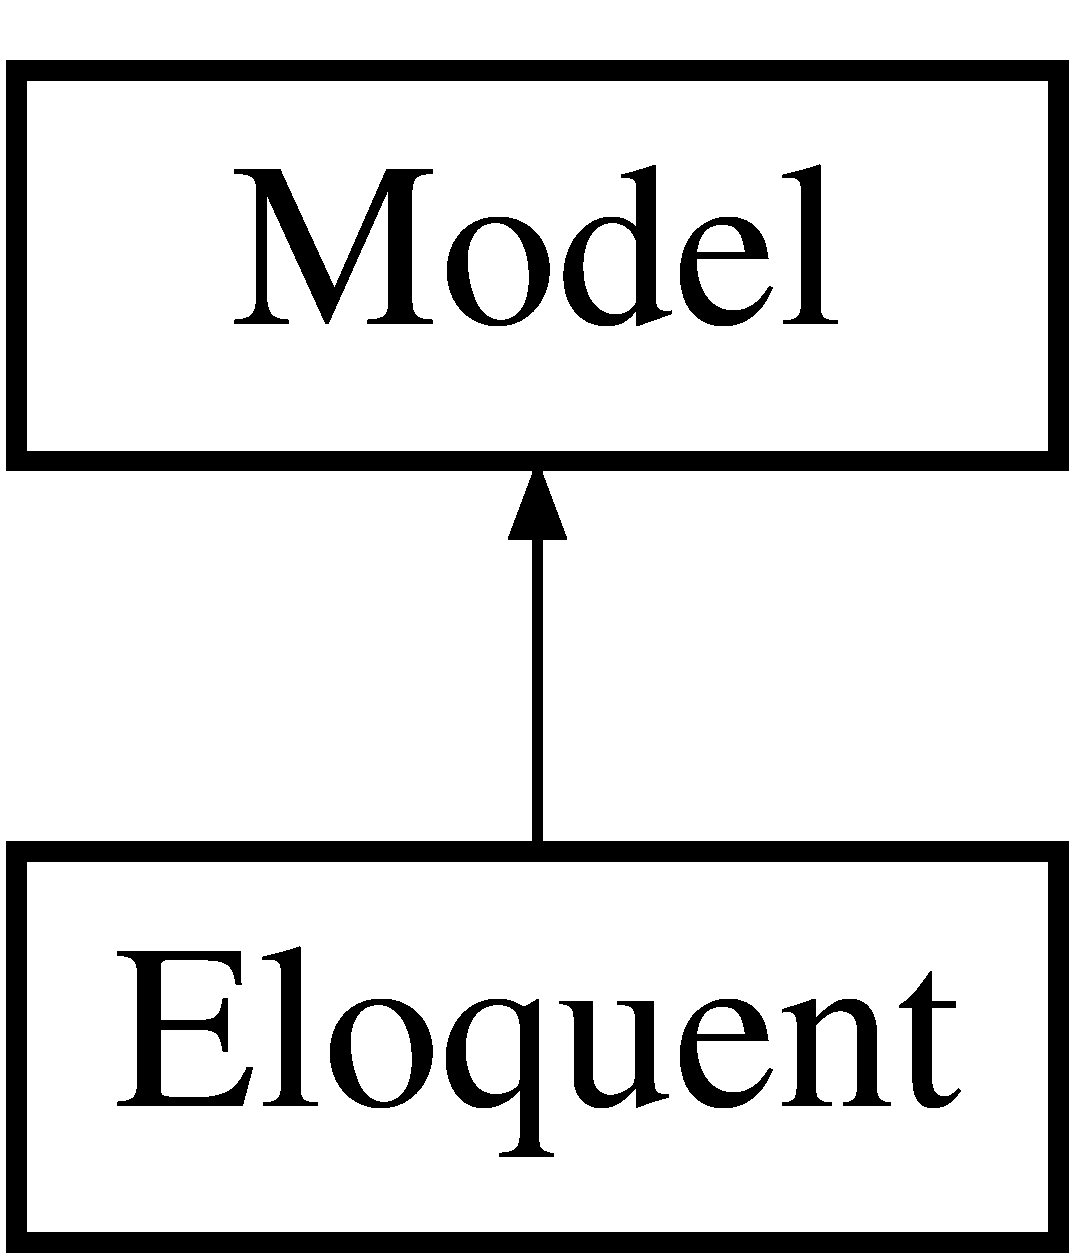
\includegraphics[height=2.000000cm]{class_eloquent}
\end{center}
\end{figure}
\subsection*{Static Public Member Functions}
\begin{DoxyCompactItemize}
\item 
static \mbox{\hyperlink{class_eloquent_a9987d6aaba201b36451caaea8065c7e4}{make}} (\$attributes=array())
\item 
static \mbox{\hyperlink{class_eloquent_a061c1fd5ab3d8e4e497f5e96a90d4ae3}{with\+Global\+Scope}} (\$identifier, \$scope)
\item 
static \mbox{\hyperlink{class_eloquent_a47d5d4f0f7be1ee5db65013ef9b79908}{without\+Global\+Scope}} (\$scope)
\item 
static \mbox{\hyperlink{class_eloquent_a65043ab2772d0ad732a64602fd6c3e2f}{without\+Global\+Scopes}} (\$\mbox{\hyperlink{class_eloquent_a30187b0aba1d255c83ca54ade893942a}{scopes}}=null)
\item 
static \mbox{\hyperlink{class_eloquent_a91d9856422b9e0ef6ea89683e6bca894}{removed\+Scopes}} ()
\item 
static \mbox{\hyperlink{class_eloquent_a99288a406c5f9d209b951ea47b09c900}{where\+Key}} (\$id)
\item 
static \mbox{\hyperlink{class_eloquent_aa270e04797f3bcd3e062ddbcbb9df59a}{where\+Key\+Not}} (\$id)
\item 
static \mbox{\hyperlink{class_eloquent_a73746da2a8ac07c59c577acde0606d5d}{where}} (\$column, \$operator=null, \$\mbox{\hyperlink{class_eloquent_a653061eb837042f61e82447886e15a72}{value}}=null, \$boolean=\textquotesingle{}and\textquotesingle{})
\item 
static \mbox{\hyperlink{class_eloquent_a24dd07936a2d5bfa885be38cf82ecb7a}{or\+Where}} (\$column, \$operator=null, \$\mbox{\hyperlink{class_eloquent_a653061eb837042f61e82447886e15a72}{value}}=null)
\item 
static \mbox{\hyperlink{class_eloquent_a4898fa742bed182f7ce97fc3301a10b2}{hydrate}} (\$items)
\item 
static \mbox{\hyperlink{class_eloquent_a5b042d9f31bce4d9423bcd5cee19e541}{from\+Query}} (\$query, \$bindings=array())
\item 
static \mbox{\hyperlink{class_eloquent_ab6ef1f841da5e0d7853767d5a35eff41}{find}} (\$id, \$columns=array())
\item 
static \mbox{\hyperlink{class_eloquent_a09565e061d998ef7b435f8b7c89af7f9}{find\+Many}} (\$ids, \$columns=array())
\item 
static \mbox{\hyperlink{class_eloquent_a5c4e81f02d09cebec4ea283bb2d14ac7}{find\+Or\+Fail}} (\$id, \$columns=array())
\item 
static \mbox{\hyperlink{class_eloquent_a5b2fd22847f1ae9772ea88792808e06b}{find\+Or\+New}} (\$id, \$columns=array())
\item 
static \mbox{\hyperlink{class_eloquent_a462f0af15dd12a99bc154d8f3808b594}{first\+Or\+New}} (\$attributes, \$values=array())
\item 
static \mbox{\hyperlink{class_eloquent_a1cbf899f6b24ec8dcd888d69bf17e21d}{first\+Or\+Create}} (\$attributes, \$values=array())
\item 
static \mbox{\hyperlink{class_eloquent_a215b8431dad0c732d5b8650df9fc1476}{update\+Or\+Create}} (\$attributes, \$values=array())
\item 
static \mbox{\hyperlink{class_eloquent_a013e6c21af18280b92abc71a1ea88763}{first\+Or\+Fail}} (\$columns=array())
\item 
static \mbox{\hyperlink{class_eloquent_a77202ee7dec38ef2364d93ed60643ede}{first\+Or}} (\$columns=array(), \$callback=null)
\item 
static \mbox{\hyperlink{class_eloquent_a653061eb837042f61e82447886e15a72}{value}} (\$column)
\item 
static \mbox{\hyperlink{class_eloquent_a6c45f389bc6894c7f4b37a8e0b9bc700}{get}} (\$columns=array())
\item 
static \mbox{\hyperlink{class_eloquent_a20abe0ed9fc973599d443fb3a9302394}{get\+Models}} (\$columns=array())
\item 
static \mbox{\hyperlink{class_eloquent_ad3df22a0761eea733b9007d0f70d3369}{eager\+Load\+Relations}} (\$models)
\item 
static \mbox{\hyperlink{class_eloquent_a7c3fb913f8b3492f3d62ed0de9e1080d}{cursor}} ()
\item 
static \mbox{\hyperlink{class_eloquent_a546b19f3697175b86e7860c186f3b592}{chunk\+By\+Id}} (\$\mbox{\hyperlink{class_eloquent_af7f114e287681eb2333c97d6bf26285d}{count}}, \$callback, \$column=null, \$alias=null)
\item 
static \mbox{\hyperlink{class_eloquent_afe73f673c6d6d904f677ecb1ab1036ae}{pluck}} (\$column, \$key=null)
\item 
static \mbox{\hyperlink{class_eloquent_a772255be01bb78f48d5e817299913aae}{paginate}} (\$per\+Page=null, \$columns=array(), \$page\+Name=\textquotesingle{}page\textquotesingle{}, \$page=null)
\item 
static \mbox{\hyperlink{class_eloquent_a62be57b10fee0b64068fe6ea7ee6f528}{simple\+Paginate}} (\$per\+Page=null, \$columns=array(), \$page\+Name=\textquotesingle{}page\textquotesingle{}, \$page=null)
\item 
static \mbox{\hyperlink{class_eloquent_af00cc719bafb53826d7adb0a4e79ed07}{create}} (\$attributes=array())
\item 
static \mbox{\hyperlink{class_eloquent_a3c4756036067296c077879f3deddbe32}{force\+Create}} (\$attributes)
\item 
static \mbox{\hyperlink{class_eloquent_a41dbb3edd9824b60aa6793e8e4f0d5de}{on\+Delete}} (\$callback)
\item 
static \mbox{\hyperlink{class_eloquent_a30187b0aba1d255c83ca54ade893942a}{scopes}} (\$scopes)
\item 
static \mbox{\hyperlink{class_eloquent_a324fd31d8a6e6391edfb691be4d2c1e4}{apply\+Scopes}} ()
\item 
static \mbox{\hyperlink{class_eloquent_a4d5bb95ee2ccbee4d66d20f96e58a2f8}{without}} (\$relations)
\item 
static \mbox{\hyperlink{class_eloquent_a8526cec0d6d3c0af7baf17035b5bcc9d}{new\+Model\+Instance}} (\$attributes=array())
\item 
static \mbox{\hyperlink{class_eloquent_a4c4d0601b74e31267f0526b02438e155}{get\+Query}} ()
\item 
static \mbox{\hyperlink{class_eloquent_a9f643b610f962c2ebc7a56cb6fcc0f71}{set\+Query}} (\$query)
\item 
static \mbox{\hyperlink{class_eloquent_abc76b992d3cb97247cd15d2d66c6e2d2}{to\+Base}} ()
\item 
static \mbox{\hyperlink{class_eloquent_a2384b7d44541eec22f7d5a34c4bac4a4}{get\+Eager\+Loads}} ()
\item 
static \mbox{\hyperlink{class_eloquent_a546bbd87b7916e506cf6d42d80ad0530}{set\+Eager\+Loads}} (\$eager\+Load)
\item 
static \mbox{\hyperlink{class_eloquent_ab711475432b10dd5e0b8992dd4b47b64}{get\+Model}} ()
\item 
static \mbox{\hyperlink{class_eloquent_af58001ac756944267c404a2ebc585cfc}{set\+Model}} (\$model)
\item 
static \mbox{\hyperlink{class_eloquent_a14eeb1ef9d588a63a99e7e2824cae2bb}{get\+Macro}} (\$name)
\item 
static \mbox{\hyperlink{class_eloquent_a48c14c8ed872ba28234c2697d75235d7}{chunk}} (\$\mbox{\hyperlink{class_eloquent_af7f114e287681eb2333c97d6bf26285d}{count}}, \$callback)
\item 
static \mbox{\hyperlink{class_eloquent_ab30a605412c7b2ba2693d4216db68ef8}{each}} (\$callback, \$\mbox{\hyperlink{class_eloquent_af7f114e287681eb2333c97d6bf26285d}{count}}=1000)
\item 
static \mbox{\hyperlink{class_eloquent_a9a02499790abaadb7a9dc307a2b8403a}{first}} (\$columns=array())
\item 
static \mbox{\hyperlink{class_eloquent_a72b824dce01f0fa80a87803b42b46ad2}{when}} (\$\mbox{\hyperlink{class_eloquent_a653061eb837042f61e82447886e15a72}{value}}, \$callback, \$default=null)
\item 
static \mbox{\hyperlink{class_eloquent_a0dd65fb10e55398ea958ac8f9a400c5e}{tap}} (\$callback)
\item 
static \mbox{\hyperlink{class_eloquent_accafe93f07a9d607402021b0c2df2c6e}{unless}} (\$\mbox{\hyperlink{class_eloquent_a653061eb837042f61e82447886e15a72}{value}}, \$callback, \$default=null)
\item 
static \mbox{\hyperlink{class_eloquent_ab786bef6379c67769eee53bb950fd389}{has}} (\$relation, \$operator=\textquotesingle{}$>$=\textquotesingle{}, \$\mbox{\hyperlink{class_eloquent_af7f114e287681eb2333c97d6bf26285d}{count}}=1, \$boolean=\textquotesingle{}and\textquotesingle{}, \$callback=null)
\item 
static \mbox{\hyperlink{class_eloquent_ab69605000942044dafd16ce8701a8565}{or\+Has}} (\$relation, \$operator=\textquotesingle{}$>$=\textquotesingle{}, \$\mbox{\hyperlink{class_eloquent_af7f114e287681eb2333c97d6bf26285d}{count}}=1)
\item 
static \mbox{\hyperlink{class_eloquent_a0856f1bda42e0b3846becb4329bf214a}{doesnt\+Have}} (\$relation, \$boolean=\textquotesingle{}and\textquotesingle{}, \$callback=null)
\item 
static \mbox{\hyperlink{class_eloquent_a00b0d5adff6b69d4b8eb864d64656a97}{or\+Doesnt\+Have}} (\$relation)
\item 
static \mbox{\hyperlink{class_eloquent_a2aa796efce7c1d1140d409b67c06f51d}{where\+Has}} (\$relation, \$callback=null, \$operator=\textquotesingle{}$>$=\textquotesingle{}, \$\mbox{\hyperlink{class_eloquent_af7f114e287681eb2333c97d6bf26285d}{count}}=1)
\item 
static \mbox{\hyperlink{class_eloquent_ae47b5731c4d49fc51c418d1b9eda590e}{or\+Where\+Has}} (\$relation, \$callback=null, \$operator=\textquotesingle{}$>$=\textquotesingle{}, \$\mbox{\hyperlink{class_eloquent_af7f114e287681eb2333c97d6bf26285d}{count}}=1)
\item 
static \mbox{\hyperlink{class_eloquent_a71116973df1571c2a9d16aa656957557}{where\+Doesnt\+Have}} (\$relation, \$callback=null)
\item 
static \mbox{\hyperlink{class_eloquent_abe51aca19cc993e96f996fa60c1c25e6}{or\+Where\+Doesnt\+Have}} (\$relation, \$callback=null)
\item 
static \mbox{\hyperlink{class_eloquent_a42b7896267dd0cee14d24f21f48ffe71}{with\+Count}} (\$relations)
\item 
static \mbox{\hyperlink{class_eloquent_a543e7d748eb32bb2b2b526c1519fe3ff}{merge\+Constraints\+From}} (\$\mbox{\hyperlink{class_eloquent_ac379856973100a47e6c99a30189be914}{from}})
\item 
static \mbox{\hyperlink{class_eloquent_a8e370395d0f8769923458070affe6569}{select}} (\$columns=array())
\item 
static \mbox{\hyperlink{class_eloquent_abaad4d45b5af66399360943de7e06088}{select\+Raw}} (\$expression, \$bindings=array())
\item 
static \mbox{\hyperlink{class_eloquent_af3d3893d466f371ddee0d6ec27fe4346}{select\+Sub}} (\$query, \$as)
\item 
static \mbox{\hyperlink{class_eloquent_af424d9b4dbb022b5320947d1d7316019}{add\+Select}} (\$column)
\item 
static \mbox{\hyperlink{class_eloquent_a0d922f51ce3d5fb3033a90a04edb2cf3}{distinct}} ()
\item 
static \mbox{\hyperlink{class_eloquent_ac379856973100a47e6c99a30189be914}{from}} (\$table)
\item 
static \mbox{\hyperlink{class_eloquent_aa041492793f1023acbce5a83b55b8cca}{join}} (\$table, \$\mbox{\hyperlink{class_eloquent_a9a02499790abaadb7a9dc307a2b8403a}{first}}, \$operator=null, \$second=null, \$type=\textquotesingle{}inner\textquotesingle{}, \$\mbox{\hyperlink{class_eloquent_a73746da2a8ac07c59c577acde0606d5d}{where}}=false)
\item 
static \mbox{\hyperlink{class_eloquent_ae729011c181ac1a0bbf3b1a8b729f4c0}{join\+Where}} (\$table, \$\mbox{\hyperlink{class_eloquent_a9a02499790abaadb7a9dc307a2b8403a}{first}}, \$operator, \$second, \$type=\textquotesingle{}inner\textquotesingle{})
\item 
static \mbox{\hyperlink{class_eloquent_aca726c1b1d75be9165046973b7fde75a}{left\+Join}} (\$table, \$\mbox{\hyperlink{class_eloquent_a9a02499790abaadb7a9dc307a2b8403a}{first}}, \$operator=null, \$second=null)
\item 
static \mbox{\hyperlink{class_eloquent_a0028d51e963f25f4e3bc2e8f8595457f}{left\+Join\+Where}} (\$table, \$\mbox{\hyperlink{class_eloquent_a9a02499790abaadb7a9dc307a2b8403a}{first}}, \$operator, \$second)
\item 
static \mbox{\hyperlink{class_eloquent_a523091b2e22ae2ec38c67cea95e6b032}{right\+Join}} (\$table, \$\mbox{\hyperlink{class_eloquent_a9a02499790abaadb7a9dc307a2b8403a}{first}}, \$operator=null, \$second=null)
\item 
static \mbox{\hyperlink{class_eloquent_a7da048e8b8edcf7c9fc154756d95217f}{right\+Join\+Where}} (\$table, \$\mbox{\hyperlink{class_eloquent_a9a02499790abaadb7a9dc307a2b8403a}{first}}, \$operator, \$second)
\item 
static \mbox{\hyperlink{class_eloquent_a8a23e4c7ff6e59bf6a8337018dcf1063}{cross\+Join}} (\$table, \$\mbox{\hyperlink{class_eloquent_a9a02499790abaadb7a9dc307a2b8403a}{first}}=null, \$operator=null, \$second=null)
\item 
static \mbox{\hyperlink{class_eloquent_ad8f6918463427fbcea1a870ec8ffd883}{merge\+Wheres}} (\$wheres, \$bindings)
\item 
static \mbox{\hyperlink{class_eloquent_a3bdca7345f418215cb3e48ccea64f8e2}{where\+Column}} (\$\mbox{\hyperlink{class_eloquent_a9a02499790abaadb7a9dc307a2b8403a}{first}}, \$operator=null, \$second=null, \$boolean=\textquotesingle{}and\textquotesingle{})
\item 
static \mbox{\hyperlink{class_eloquent_a7fb5678acda4390052f891418895762a}{or\+Where\+Column}} (\$\mbox{\hyperlink{class_eloquent_a9a02499790abaadb7a9dc307a2b8403a}{first}}, \$operator=null, \$second=null)
\item 
static \mbox{\hyperlink{class_eloquent_a67c4e71aff7e9c4304516de058845610}{where\+Raw}} (\$sql, \$bindings=array(), \$boolean=\textquotesingle{}and\textquotesingle{})
\item 
static \mbox{\hyperlink{class_eloquent_afbe643f67e54beddea0721074a50093e}{or\+Where\+Raw}} (\$sql, \$bindings=array())
\item 
static \mbox{\hyperlink{class_eloquent_ae4274acd45de3339f0718ad3fa0fea34}{where\+In}} (\$column, \$values, \$boolean=\textquotesingle{}and\textquotesingle{}, \$not=false)
\item 
static \mbox{\hyperlink{class_eloquent_ac49cc6a793b16ab8edc3eb0b91d0c355}{or\+Where\+In}} (\$column, \$values)
\item 
static \mbox{\hyperlink{class_eloquent_aea049d383c88e86dc7456fb0aed328f5}{where\+Not\+In}} (\$column, \$values, \$boolean=\textquotesingle{}and\textquotesingle{})
\item 
static \mbox{\hyperlink{class_eloquent_a07382bcdd1d4e66e2440cc1c5f5ba77b}{or\+Where\+Not\+In}} (\$column, \$values)
\item 
static \mbox{\hyperlink{class_eloquent_ae53f3a49e729b996083e5d835f737e23}{where\+Null}} (\$column, \$boolean=\textquotesingle{}and\textquotesingle{}, \$not=false)
\item 
static \mbox{\hyperlink{class_eloquent_ad05158229fe7106000cde4d97cb07537}{or\+Where\+Null}} (\$column)
\item 
static \mbox{\hyperlink{class_eloquent_a16cb0cdb621e7bfeec2cd87af4a224db}{where\+Not\+Null}} (\$column, \$boolean=\textquotesingle{}and\textquotesingle{})
\item 
static \mbox{\hyperlink{class_eloquent_a4fa71165cd2667a557c0125fa3292896}{where\+Between}} (\$column, \$values, \$boolean=\textquotesingle{}and\textquotesingle{}, \$not=false)
\item 
static \mbox{\hyperlink{class_eloquent_a0e1487272eea316ffc9019c50e8aa025}{or\+Where\+Between}} (\$column, \$values)
\item 
static \mbox{\hyperlink{class_eloquent_aa337ce79cac3593ee4c6fdf072b3528d}{where\+Not\+Between}} (\$column, \$values, \$boolean=\textquotesingle{}and\textquotesingle{})
\item 
static \mbox{\hyperlink{class_eloquent_a17c4940b6622bb7210567714b237b23a}{or\+Where\+Not\+Between}} (\$column, \$values)
\item 
static \mbox{\hyperlink{class_eloquent_a0f49fc5796ee0ed0b9d8c8bda60718e4}{or\+Where\+Not\+Null}} (\$column)
\item 
static \mbox{\hyperlink{class_eloquent_a5f295e03df6a9022fa12ce9a1607d08d}{where\+Date}} (\$column, \$operator, \$\mbox{\hyperlink{class_eloquent_a653061eb837042f61e82447886e15a72}{value}}=null, \$boolean=\textquotesingle{}and\textquotesingle{})
\item 
static \mbox{\hyperlink{class_eloquent_abac95061fffa73cb51b275e5ee5fa09a}{or\+Where\+Date}} (\$column, \$operator, \$\mbox{\hyperlink{class_eloquent_a653061eb837042f61e82447886e15a72}{value}})
\item 
static \mbox{\hyperlink{class_eloquent_ac534556e3ff4230a01e36cf6c4131cc7}{where\+Time}} (\$column, \$operator, \$\mbox{\hyperlink{class_eloquent_a653061eb837042f61e82447886e15a72}{value}}, \$boolean=\textquotesingle{}and\textquotesingle{})
\item 
static \mbox{\hyperlink{class_eloquent_a00cf4a8d42cc19861a94719dbb5177e4}{or\+Where\+Time}} (\$column, \$operator, \$\mbox{\hyperlink{class_eloquent_a653061eb837042f61e82447886e15a72}{value}})
\item 
static \mbox{\hyperlink{class_eloquent_a8442c6da11bda9fe1fad7b412ce48ec9}{where\+Day}} (\$column, \$operator, \$\mbox{\hyperlink{class_eloquent_a653061eb837042f61e82447886e15a72}{value}}=null, \$boolean=\textquotesingle{}and\textquotesingle{})
\item 
static \mbox{\hyperlink{class_eloquent_a530752faf5aed57517a152e74eceffd3}{where\+Month}} (\$column, \$operator, \$\mbox{\hyperlink{class_eloquent_a653061eb837042f61e82447886e15a72}{value}}=null, \$boolean=\textquotesingle{}and\textquotesingle{})
\item 
static \mbox{\hyperlink{class_eloquent_a02fd683aa7d0c0159379f8d3b27d5230}{where\+Year}} (\$column, \$operator, \$\mbox{\hyperlink{class_eloquent_a653061eb837042f61e82447886e15a72}{value}}=null, \$boolean=\textquotesingle{}and\textquotesingle{})
\item 
static \mbox{\hyperlink{class_eloquent_a1e91f1cb7ebaef1a1dac7aef95a95916}{where\+Nested}} (\$callback, \$boolean=\textquotesingle{}and\textquotesingle{})
\item 
static \mbox{\hyperlink{class_eloquent_a73ee05439dd72e88926cd48a01b2ba6b}{for\+Nested\+Where}} ()
\item 
static \mbox{\hyperlink{class_eloquent_aa2f16128ef6e7142fc3a0fcf2c4590a0}{add\+Nested\+Where\+Query}} (\$query, \$boolean=\textquotesingle{}and\textquotesingle{})
\item 
static \mbox{\hyperlink{class_eloquent_abe35963f00cb4cbba9c09bf9c7a36881}{where\+Exists}} (\$callback, \$boolean=\textquotesingle{}and\textquotesingle{}, \$not=false)
\item 
static \mbox{\hyperlink{class_eloquent_a461302857867cda6902c6fcaa9581d67}{or\+Where\+Exists}} (\$callback, \$not=false)
\item 
static \mbox{\hyperlink{class_eloquent_aa2b4f08f03816e520e6f55d21ca49c06}{where\+Not\+Exists}} (\$callback, \$boolean=\textquotesingle{}and\textquotesingle{})
\item 
static \mbox{\hyperlink{class_eloquent_a0b8b11378bd5bdfcc39a9879a54adacf}{or\+Where\+Not\+Exists}} (\$callback)
\item 
static \mbox{\hyperlink{class_eloquent_aa890d018e0ad839b0bb5a2c2d243243c}{add\+Where\+Exists\+Query}} (\$query, \$boolean=\textquotesingle{}and\textquotesingle{}, \$not=false)
\item 
static \mbox{\hyperlink{class_eloquent_a92ee7d621c7c646a0e2da14be557ec53}{dynamic\+Where}} (\$method, \$parameters)
\item 
static \mbox{\hyperlink{class_eloquent_aeebb6f260f6d6fd5afab7b02ff15248a}{group\+By}} (\$groups=null)
\item 
static \mbox{\hyperlink{class_eloquent_a1a90ee18a28cc2930fbf1ba43e7a8736}{having}} (\$column, \$operator=null, \$\mbox{\hyperlink{class_eloquent_a653061eb837042f61e82447886e15a72}{value}}=null, \$boolean=\textquotesingle{}and\textquotesingle{})
\item 
static \mbox{\hyperlink{class_eloquent_a5dec38cf2c59fd1fd2f1aeba5508e0cc}{or\+Having}} (\$column, \$operator=null, \$\mbox{\hyperlink{class_eloquent_a653061eb837042f61e82447886e15a72}{value}}=null)
\item 
static \mbox{\hyperlink{class_eloquent_a756265cf9b44ab3d9d63a5364763d9f2}{having\+Raw}} (\$sql, \$bindings=array(), \$boolean=\textquotesingle{}and\textquotesingle{})
\item 
static \mbox{\hyperlink{class_eloquent_a6fac6b159c4a57120d5a6ac77cbca16c}{or\+Having\+Raw}} (\$sql, \$bindings=array())
\item 
static \mbox{\hyperlink{class_eloquent_a892149342bab8cc0e624dd009c0aaa01}{order\+By}} (\$column, \$direction=\textquotesingle{}asc\textquotesingle{})
\item 
static \mbox{\hyperlink{class_eloquent_af93c2d362571fd37e1e7cf33aa627a0a}{order\+By\+Desc}} (\$column)
\item 
static \mbox{\hyperlink{class_eloquent_a6ece4c9b56f9334272522c306f283a2f}{latest}} (\$column=\textquotesingle{}created\+\_\+at\textquotesingle{})
\item 
static \mbox{\hyperlink{class_eloquent_a3a6232dc598b629da754e20f19a02a81}{oldest}} (\$column=\textquotesingle{}created\+\_\+at\textquotesingle{})
\item 
static \mbox{\hyperlink{class_eloquent_a75919dc1a77ec126c2188aa97c890b45}{in\+Random\+Order}} (\$seed=\textquotesingle{}\textquotesingle{})
\item 
static \mbox{\hyperlink{class_eloquent_a817e3e9e4221b1bb88b1c5bc57e18c3c}{order\+By\+Raw}} (\$sql, \$bindings=array())
\item 
static \mbox{\hyperlink{class_eloquent_a2fd45cfad88ad5d4d5a2a77920cabfcf}{skip}} (\$\mbox{\hyperlink{class_eloquent_a653061eb837042f61e82447886e15a72}{value}})
\item 
static \mbox{\hyperlink{class_eloquent_ab8f792a4282a6d9fb5897ef7eb066dda}{offset}} (\$\mbox{\hyperlink{class_eloquent_a653061eb837042f61e82447886e15a72}{value}})
\item 
static \mbox{\hyperlink{class_eloquent_ae3c0357543a8e9d871ca61bf64109793}{take}} (\$\mbox{\hyperlink{class_eloquent_a653061eb837042f61e82447886e15a72}{value}})
\item 
static \mbox{\hyperlink{class_eloquent_a4c6d298be10cf541f36b4c50311cd8cc}{limit}} (\$\mbox{\hyperlink{class_eloquent_a653061eb837042f61e82447886e15a72}{value}})
\item 
static \mbox{\hyperlink{class_eloquent_a6bcc6951a0901e619a303e777ec1d971}{for\+Page}} (\$page, \$per\+Page=15)
\item 
static \mbox{\hyperlink{class_eloquent_ac7f037ea162597f9d44b8e9010e60c77}{for\+Page\+After\+Id}} (\$per\+Page=15, \$last\+Id=0, \$column=\textquotesingle{}id\textquotesingle{})
\item 
static \mbox{\hyperlink{class_eloquent_a24685bd0575b3a51452944bee875b83c}{union}} (\$query, \$all=false)
\item 
static \mbox{\hyperlink{class_eloquent_a7a81a35976fe17001e5a7ffad92f5256}{union\+All}} (\$query)
\item 
static \mbox{\hyperlink{class_eloquent_a99a6223b6ef3008aff9b1d113f67449f}{lock}} (\$\mbox{\hyperlink{class_eloquent_a653061eb837042f61e82447886e15a72}{value}}=true)
\item 
static \mbox{\hyperlink{class_eloquent_a8424881c1216eeb0bf339b38c713a090}{lock\+For\+Update}} ()
\item 
static \mbox{\hyperlink{class_eloquent_a7f299b24133d1b7b5614210b34907801}{shared\+Lock}} ()
\item 
static \mbox{\hyperlink{class_eloquent_ac788e862f43bba3f9d0ff6a13b82774b}{to\+Sql}} ()
\item 
static \mbox{\hyperlink{class_eloquent_a1978abdf53fe44de908f19767234e984}{get\+Count\+For\+Pagination}} (\$columns=array())
\item 
static \mbox{\hyperlink{class_eloquent_a61e6ba8ce2c591132da5397c88b976b9}{implode}} (\$column, \$glue=\textquotesingle{}\textquotesingle{})
\item 
static \mbox{\hyperlink{class_eloquent_a0778402ef6d4010610378d9a470e6d4b}{exists}} ()
\item 
static \mbox{\hyperlink{class_eloquent_af7f114e287681eb2333c97d6bf26285d}{count}} (\$columns=\textquotesingle{} $\ast$\textquotesingle{})
\item 
static \mbox{\hyperlink{class_eloquent_a0c9b274069dc6503f3ac3d7592c7c69d}{min}} (\$column)
\item 
static \mbox{\hyperlink{class_eloquent_a74732442e996af19bbb46d839a6fddf3}{max}} (\$column)
\item 
static \mbox{\hyperlink{class_eloquent_a74c6b202fd0d2f82c2dc9a326ab4f8fc}{sum}} (\$column)
\item 
static \mbox{\hyperlink{class_eloquent_a0b3828a100dd3fdcb15a5df6bc4c0f16}{avg}} (\$column)
\item 
static \mbox{\hyperlink{class_eloquent_a7ad1944b3c3cc2e9f11b9d028ffa5501}{average}} (\$column)
\item 
static \mbox{\hyperlink{class_eloquent_abebad76dc3dba8a1894b8a2554e0a4ff}{aggregate}} (\$function, \$columns=array())
\item 
static \mbox{\hyperlink{class_eloquent_ae0d141ad31eacf1a97177bb8b1e896e0}{numeric\+Aggregate}} (\$function, \$columns=array())
\item 
static \mbox{\hyperlink{class_eloquent_af7d0fbced37746ae8bd902ef5f68a7ae}{insert}} (\$values)
\item 
static \mbox{\hyperlink{class_eloquent_a1844f44a1ce5e328d145034b7536e2ea}{insert\+Get\+Id}} (\$values, \$sequence=null)
\item 
static \mbox{\hyperlink{class_eloquent_a9000a3ec879c46fbd69d07e9818da617}{update\+Or\+Insert}} (\$attributes, \$values=array())
\item 
static \mbox{\hyperlink{class_eloquent_a96ac4ef3c15f8420f7517ef3a5c75b8c}{truncate}} ()
\item 
static \mbox{\hyperlink{class_eloquent_a526a8894771e444ed5aa81987eecd3cf}{raw}} (\$\mbox{\hyperlink{class_eloquent_a653061eb837042f61e82447886e15a72}{value}})
\item 
static \mbox{\hyperlink{class_eloquent_a2354a3b999001c7332d956e5cc2fcf07}{get\+Bindings}} ()
\item 
static \mbox{\hyperlink{class_eloquent_a0e2f203149983e1293a215f5d010e014}{get\+Raw\+Bindings}} ()
\item 
static \mbox{\hyperlink{class_eloquent_a3ce121762513ed5de49b13594887f51c}{set\+Bindings}} (\$bindings, \$type=\textquotesingle{}\mbox{\hyperlink{class_eloquent_a73746da2a8ac07c59c577acde0606d5d}{where}}\textquotesingle{})
\item 
static \mbox{\hyperlink{class_eloquent_ab657124a93444b0a941f40d943bac574}{add\+Binding}} (\$\mbox{\hyperlink{class_eloquent_a653061eb837042f61e82447886e15a72}{value}}, \$type=\textquotesingle{}\mbox{\hyperlink{class_eloquent_a73746da2a8ac07c59c577acde0606d5d}{where}}\textquotesingle{})
\item 
static \mbox{\hyperlink{class_eloquent_a590622affbe9e982b13019733af32012}{merge\+Bindings}} (\$query)
\item 
static \mbox{\hyperlink{class_eloquent_af06482fd0045347d96e02da15e1bcd2c}{get\+Processor}} ()
\item 
static \mbox{\hyperlink{class_eloquent_ad1d4b842e0773138ab7660b968cc180b}{get\+Grammar}} ()
\item 
static \mbox{\hyperlink{class_eloquent_a8e99b1a02f0cb83410036aea50c23b24}{use\+Write\+Pdo}} ()
\item 
static \mbox{\hyperlink{class_eloquent_acbd1833f18473cd1dd4fb755460592f3}{clone\+Without}} (\$properties)
\item 
static \mbox{\hyperlink{class_eloquent_a3794141227f450194be39fe46372cfa3}{clone\+Without\+Bindings}} (\$except)
\item 
static \mbox{\hyperlink{class_eloquent_a8839c902460bd7744993f61693711cf7}{macro}} (\$name, \$macro)
\item 
static \mbox{\hyperlink{class_eloquent_a59e9f5c02a0686de57f66eeb0230df58}{mixin}} (\$mixin)
\item 
static \mbox{\hyperlink{class_eloquent_a02e81dba5c768e3cb30a0394d697582a}{has\+Macro}} (\$name)
\item 
static \mbox{\hyperlink{class_eloquent_a6afe5c89170eab3d8de7693f741accfa}{macro\+Call}} (\$method, \$parameters)
\end{DoxyCompactItemize}


\subsection{Member Function Documentation}
\mbox{\Hypertarget{class_eloquent_ab657124a93444b0a941f40d943bac574}\label{class_eloquent_ab657124a93444b0a941f40d943bac574}} 
\index{Eloquent@{Eloquent}!add\+Binding@{add\+Binding}}
\index{add\+Binding@{add\+Binding}!Eloquent@{Eloquent}}
\subsubsection{\texorpdfstring{add\+Binding()}{addBinding()}}
{\footnotesize\ttfamily static Eloquent\+::add\+Binding (\begin{DoxyParamCaption}\item[{}]{\$value,  }\item[{}]{\$type = {\ttfamily \textquotesingle{}\mbox{\hyperlink{class_eloquent_a73746da2a8ac07c59c577acde0606d5d}{where}}\textquotesingle{}} }\end{DoxyParamCaption})\hspace{0.3cm}{\ttfamily [static]}}

Add a binding to the query.


\begin{DoxyParams}[1]{Parameters}
mixed & {\em \$value} & \\
\hline
string & {\em \$type} & \\
\hline
\end{DoxyParams}
\begin{DoxyReturn}{Returns}
\$this 
\end{DoxyReturn}

\begin{DoxyExceptions}{Exceptions}
{\em } & \\
\hline
\end{DoxyExceptions}
\mbox{\Hypertarget{class_eloquent_aa2f16128ef6e7142fc3a0fcf2c4590a0}\label{class_eloquent_aa2f16128ef6e7142fc3a0fcf2c4590a0}} 
\index{Eloquent@{Eloquent}!add\+Nested\+Where\+Query@{add\+Nested\+Where\+Query}}
\index{add\+Nested\+Where\+Query@{add\+Nested\+Where\+Query}!Eloquent@{Eloquent}}
\subsubsection{\texorpdfstring{add\+Nested\+Where\+Query()}{addNestedWhereQuery()}}
{\footnotesize\ttfamily static Eloquent\+::add\+Nested\+Where\+Query (\begin{DoxyParamCaption}\item[{}]{\$query,  }\item[{}]{\$boolean = {\ttfamily \textquotesingle{}and\textquotesingle{}} }\end{DoxyParamCaption})\hspace{0.3cm}{\ttfamily [static]}}

Add another query builder as a nested where to the query builder.


\begin{DoxyParams}[1]{Parameters}
\textbackslash{}\+Illuminate\textbackslash{}\+Database\textbackslash{}\+Query\textbackslash{}\+Builder | static & {\em \$query} & \\
\hline
string & {\em \$boolean} & \\
\hline
\end{DoxyParams}
\begin{DoxyReturn}{Returns}
\$this 
\end{DoxyReturn}
\mbox{\Hypertarget{class_eloquent_af424d9b4dbb022b5320947d1d7316019}\label{class_eloquent_af424d9b4dbb022b5320947d1d7316019}} 
\index{Eloquent@{Eloquent}!add\+Select@{add\+Select}}
\index{add\+Select@{add\+Select}!Eloquent@{Eloquent}}
\subsubsection{\texorpdfstring{add\+Select()}{addSelect()}}
{\footnotesize\ttfamily static Eloquent\+::add\+Select (\begin{DoxyParamCaption}\item[{}]{\$column }\end{DoxyParamCaption})\hspace{0.3cm}{\ttfamily [static]}}

Add a new select column to the query.


\begin{DoxyParams}[1]{Parameters}
array | mixed & {\em \$column} & \\
\hline
\end{DoxyParams}
\begin{DoxyReturn}{Returns}
\$this 
\end{DoxyReturn}
\mbox{\Hypertarget{class_eloquent_aa890d018e0ad839b0bb5a2c2d243243c}\label{class_eloquent_aa890d018e0ad839b0bb5a2c2d243243c}} 
\index{Eloquent@{Eloquent}!add\+Where\+Exists\+Query@{add\+Where\+Exists\+Query}}
\index{add\+Where\+Exists\+Query@{add\+Where\+Exists\+Query}!Eloquent@{Eloquent}}
\subsubsection{\texorpdfstring{add\+Where\+Exists\+Query()}{addWhereExistsQuery()}}
{\footnotesize\ttfamily static Eloquent\+::add\+Where\+Exists\+Query (\begin{DoxyParamCaption}\item[{}]{\$query,  }\item[{}]{\$boolean = {\ttfamily \textquotesingle{}and\textquotesingle{}},  }\item[{}]{\$not = {\ttfamily false} }\end{DoxyParamCaption})\hspace{0.3cm}{\ttfamily [static]}}

Add an exists clause to the query.


\begin{DoxyParams}[1]{Parameters}
\textbackslash{}\+Illuminate\textbackslash{}\+Database\textbackslash{}\+Query\textbackslash{}\+Builder & {\em \$query} & \\
\hline
string & {\em \$boolean} & \\
\hline
bool & {\em \$not} & \\
\hline
\end{DoxyParams}
\begin{DoxyReturn}{Returns}
\$this 
\end{DoxyReturn}
\mbox{\Hypertarget{class_eloquent_abebad76dc3dba8a1894b8a2554e0a4ff}\label{class_eloquent_abebad76dc3dba8a1894b8a2554e0a4ff}} 
\index{Eloquent@{Eloquent}!aggregate@{aggregate}}
\index{aggregate@{aggregate}!Eloquent@{Eloquent}}
\subsubsection{\texorpdfstring{aggregate()}{aggregate()}}
{\footnotesize\ttfamily static Eloquent\+::aggregate (\begin{DoxyParamCaption}\item[{}]{\$function,  }\item[{}]{\$columns = {\ttfamily array()} }\end{DoxyParamCaption})\hspace{0.3cm}{\ttfamily [static]}}

Execute an aggregate function on the database.


\begin{DoxyParams}[1]{Parameters}
string & {\em \$function} & \\
\hline
array & {\em \$columns} & \\
\hline
\end{DoxyParams}
\begin{DoxyReturn}{Returns}
mixed 
\end{DoxyReturn}
\mbox{\Hypertarget{class_eloquent_a324fd31d8a6e6391edfb691be4d2c1e4}\label{class_eloquent_a324fd31d8a6e6391edfb691be4d2c1e4}} 
\index{Eloquent@{Eloquent}!apply\+Scopes@{apply\+Scopes}}
\index{apply\+Scopes@{apply\+Scopes}!Eloquent@{Eloquent}}
\subsubsection{\texorpdfstring{apply\+Scopes()}{applyScopes()}}
{\footnotesize\ttfamily static Eloquent\+::apply\+Scopes (\begin{DoxyParamCaption}{ }\end{DoxyParamCaption})\hspace{0.3cm}{\ttfamily [static]}}

Apply the scopes to the \mbox{\hyperlink{class_eloquent}{Eloquent}} builder instance and return it.

\begin{DoxyReturn}{Returns}
$\vert$static 
\end{DoxyReturn}
\mbox{\Hypertarget{class_eloquent_a7ad1944b3c3cc2e9f11b9d028ffa5501}\label{class_eloquent_a7ad1944b3c3cc2e9f11b9d028ffa5501}} 
\index{Eloquent@{Eloquent}!average@{average}}
\index{average@{average}!Eloquent@{Eloquent}}
\subsubsection{\texorpdfstring{average()}{average()}}
{\footnotesize\ttfamily static Eloquent\+::average (\begin{DoxyParamCaption}\item[{}]{\$column }\end{DoxyParamCaption})\hspace{0.3cm}{\ttfamily [static]}}

Alias for the \char`\"{}avg\char`\"{} method.


\begin{DoxyParams}[1]{Parameters}
string & {\em \$column} & \\
\hline
\end{DoxyParams}
\begin{DoxyReturn}{Returns}
mixed 
\end{DoxyReturn}
\mbox{\Hypertarget{class_eloquent_a0b3828a100dd3fdcb15a5df6bc4c0f16}\label{class_eloquent_a0b3828a100dd3fdcb15a5df6bc4c0f16}} 
\index{Eloquent@{Eloquent}!avg@{avg}}
\index{avg@{avg}!Eloquent@{Eloquent}}
\subsubsection{\texorpdfstring{avg()}{avg()}}
{\footnotesize\ttfamily static Eloquent\+::avg (\begin{DoxyParamCaption}\item[{}]{\$column }\end{DoxyParamCaption})\hspace{0.3cm}{\ttfamily [static]}}

Retrieve the average of the values of a given column.


\begin{DoxyParams}[1]{Parameters}
string & {\em \$column} & \\
\hline
\end{DoxyParams}
\begin{DoxyReturn}{Returns}
mixed 
\end{DoxyReturn}
\mbox{\Hypertarget{class_eloquent_a48c14c8ed872ba28234c2697d75235d7}\label{class_eloquent_a48c14c8ed872ba28234c2697d75235d7}} 
\index{Eloquent@{Eloquent}!chunk@{chunk}}
\index{chunk@{chunk}!Eloquent@{Eloquent}}
\subsubsection{\texorpdfstring{chunk()}{chunk()}}
{\footnotesize\ttfamily static Eloquent\+::chunk (\begin{DoxyParamCaption}\item[{}]{\$count,  }\item[{}]{\$callback }\end{DoxyParamCaption})\hspace{0.3cm}{\ttfamily [static]}}

Chunk the results of the query.


\begin{DoxyParams}[1]{Parameters}
int & {\em \$count} & \\
\hline
callable & {\em \$callback} & \\
\hline
\end{DoxyParams}
\begin{DoxyReturn}{Returns}
bool 
\end{DoxyReturn}
\mbox{\Hypertarget{class_eloquent_a546b19f3697175b86e7860c186f3b592}\label{class_eloquent_a546b19f3697175b86e7860c186f3b592}} 
\index{Eloquent@{Eloquent}!chunk\+By\+Id@{chunk\+By\+Id}}
\index{chunk\+By\+Id@{chunk\+By\+Id}!Eloquent@{Eloquent}}
\subsubsection{\texorpdfstring{chunk\+By\+Id()}{chunkById()}}
{\footnotesize\ttfamily static Eloquent\+::chunk\+By\+Id (\begin{DoxyParamCaption}\item[{}]{\$count,  }\item[{}]{\$callback,  }\item[{}]{\$column = {\ttfamily null},  }\item[{}]{\$alias = {\ttfamily null} }\end{DoxyParamCaption})\hspace{0.3cm}{\ttfamily [static]}}

Chunk the results of a query by comparing numeric I\+Ds.


\begin{DoxyParams}[1]{Parameters}
int & {\em \$count} & \\
\hline
callable & {\em \$callback} & \\
\hline
string & {\em \$column} & \\
\hline
string | null & {\em \$alias} & \\
\hline
\end{DoxyParams}
\begin{DoxyReturn}{Returns}
bool 
\end{DoxyReturn}
\mbox{\Hypertarget{class_eloquent_acbd1833f18473cd1dd4fb755460592f3}\label{class_eloquent_acbd1833f18473cd1dd4fb755460592f3}} 
\index{Eloquent@{Eloquent}!clone\+Without@{clone\+Without}}
\index{clone\+Without@{clone\+Without}!Eloquent@{Eloquent}}
\subsubsection{\texorpdfstring{clone\+Without()}{cloneWithout()}}
{\footnotesize\ttfamily static Eloquent\+::clone\+Without (\begin{DoxyParamCaption}\item[{}]{\$properties }\end{DoxyParamCaption})\hspace{0.3cm}{\ttfamily [static]}}

Clone the query without the given properties.


\begin{DoxyParams}[1]{Parameters}
array & {\em \$properties} & \\
\hline
\end{DoxyParams}
\begin{DoxyReturn}{Returns}
static 
\end{DoxyReturn}
\mbox{\Hypertarget{class_eloquent_a3794141227f450194be39fe46372cfa3}\label{class_eloquent_a3794141227f450194be39fe46372cfa3}} 
\index{Eloquent@{Eloquent}!clone\+Without\+Bindings@{clone\+Without\+Bindings}}
\index{clone\+Without\+Bindings@{clone\+Without\+Bindings}!Eloquent@{Eloquent}}
\subsubsection{\texorpdfstring{clone\+Without\+Bindings()}{cloneWithoutBindings()}}
{\footnotesize\ttfamily static Eloquent\+::clone\+Without\+Bindings (\begin{DoxyParamCaption}\item[{}]{\$except }\end{DoxyParamCaption})\hspace{0.3cm}{\ttfamily [static]}}

Clone the query without the given bindings.


\begin{DoxyParams}[1]{Parameters}
array & {\em \$except} & \\
\hline
\end{DoxyParams}
\begin{DoxyReturn}{Returns}
static 
\end{DoxyReturn}
\mbox{\Hypertarget{class_eloquent_af7f114e287681eb2333c97d6bf26285d}\label{class_eloquent_af7f114e287681eb2333c97d6bf26285d}} 
\index{Eloquent@{Eloquent}!count@{count}}
\index{count@{count}!Eloquent@{Eloquent}}
\subsubsection{\texorpdfstring{count()}{count()}}
{\footnotesize\ttfamily static Eloquent\+::count (\begin{DoxyParamCaption}\item[{}]{\$columns = {\ttfamily \textquotesingle{}$\ast$\textquotesingle{}} }\end{DoxyParamCaption})\hspace{0.3cm}{\ttfamily [static]}}

Retrieve the \char`\"{}count\char`\"{} result of the query.


\begin{DoxyParams}[1]{Parameters}
string & {\em \$columns} & \\
\hline
\end{DoxyParams}
\begin{DoxyReturn}{Returns}
int 
\end{DoxyReturn}
\mbox{\Hypertarget{class_eloquent_af00cc719bafb53826d7adb0a4e79ed07}\label{class_eloquent_af00cc719bafb53826d7adb0a4e79ed07}} 
\index{Eloquent@{Eloquent}!create@{create}}
\index{create@{create}!Eloquent@{Eloquent}}
\subsubsection{\texorpdfstring{create()}{create()}}
{\footnotesize\ttfamily static Eloquent\+::create (\begin{DoxyParamCaption}\item[{}]{\$attributes = {\ttfamily array()} }\end{DoxyParamCaption})\hspace{0.3cm}{\ttfamily [static]}}

Save a new model and return the instance.


\begin{DoxyParams}[1]{Parameters}
array & {\em \$attributes} & \\
\hline
\end{DoxyParams}
\begin{DoxyReturn}{Returns}
$\vert$\$this 
\end{DoxyReturn}
\mbox{\Hypertarget{class_eloquent_a8a23e4c7ff6e59bf6a8337018dcf1063}\label{class_eloquent_a8a23e4c7ff6e59bf6a8337018dcf1063}} 
\index{Eloquent@{Eloquent}!cross\+Join@{cross\+Join}}
\index{cross\+Join@{cross\+Join}!Eloquent@{Eloquent}}
\subsubsection{\texorpdfstring{cross\+Join()}{crossJoin()}}
{\footnotesize\ttfamily static Eloquent\+::cross\+Join (\begin{DoxyParamCaption}\item[{}]{\$table,  }\item[{}]{\$first = {\ttfamily null},  }\item[{}]{\$operator = {\ttfamily null},  }\item[{}]{\$second = {\ttfamily null} }\end{DoxyParamCaption})\hspace{0.3cm}{\ttfamily [static]}}

Add a \char`\"{}cross join\char`\"{} clause to the query.


\begin{DoxyParams}[1]{Parameters}
string & {\em \$table} & \\
\hline
string | null & {\em \$first} & \\
\hline
string | null & {\em \$operator} & \\
\hline
string | null & {\em \$second} & \\
\hline
\end{DoxyParams}
\begin{DoxyReturn}{Returns}
$\vert$static 
\end{DoxyReturn}
\mbox{\Hypertarget{class_eloquent_a7c3fb913f8b3492f3d62ed0de9e1080d}\label{class_eloquent_a7c3fb913f8b3492f3d62ed0de9e1080d}} 
\index{Eloquent@{Eloquent}!cursor@{cursor}}
\index{cursor@{cursor}!Eloquent@{Eloquent}}
\subsubsection{\texorpdfstring{cursor()}{cursor()}}
{\footnotesize\ttfamily static Eloquent\+::cursor (\begin{DoxyParamCaption}{ }\end{DoxyParamCaption})\hspace{0.3cm}{\ttfamily [static]}}

Get a generator for the given query.

\begin{DoxyReturn}{Returns}

\end{DoxyReturn}
\mbox{\Hypertarget{class_eloquent_a0d922f51ce3d5fb3033a90a04edb2cf3}\label{class_eloquent_a0d922f51ce3d5fb3033a90a04edb2cf3}} 
\index{Eloquent@{Eloquent}!distinct@{distinct}}
\index{distinct@{distinct}!Eloquent@{Eloquent}}
\subsubsection{\texorpdfstring{distinct()}{distinct()}}
{\footnotesize\ttfamily static Eloquent\+::distinct (\begin{DoxyParamCaption}{ }\end{DoxyParamCaption})\hspace{0.3cm}{\ttfamily [static]}}

Force the query to only return distinct results.

\begin{DoxyReturn}{Returns}
\$this 
\end{DoxyReturn}
\mbox{\Hypertarget{class_eloquent_a0856f1bda42e0b3846becb4329bf214a}\label{class_eloquent_a0856f1bda42e0b3846becb4329bf214a}} 
\index{Eloquent@{Eloquent}!doesnt\+Have@{doesnt\+Have}}
\index{doesnt\+Have@{doesnt\+Have}!Eloquent@{Eloquent}}
\subsubsection{\texorpdfstring{doesnt\+Have()}{doesntHave()}}
{\footnotesize\ttfamily static Eloquent\+::doesnt\+Have (\begin{DoxyParamCaption}\item[{}]{\$relation,  }\item[{}]{\$boolean = {\ttfamily \textquotesingle{}and\textquotesingle{}},  }\item[{}]{\$callback = {\ttfamily null} }\end{DoxyParamCaption})\hspace{0.3cm}{\ttfamily [static]}}

Add a relationship count / exists condition to the query.


\begin{DoxyParams}[1]{Parameters}
string & {\em \$relation} & \\
\hline
string & {\em \$boolean} & \\
\hline
\textbackslash{}\+Closure | null & {\em \$callback} & \\
\hline
\end{DoxyParams}
\begin{DoxyReturn}{Returns}
$\vert$static 
\end{DoxyReturn}
\mbox{\Hypertarget{class_eloquent_a92ee7d621c7c646a0e2da14be557ec53}\label{class_eloquent_a92ee7d621c7c646a0e2da14be557ec53}} 
\index{Eloquent@{Eloquent}!dynamic\+Where@{dynamic\+Where}}
\index{dynamic\+Where@{dynamic\+Where}!Eloquent@{Eloquent}}
\subsubsection{\texorpdfstring{dynamic\+Where()}{dynamicWhere()}}
{\footnotesize\ttfamily static Eloquent\+::dynamic\+Where (\begin{DoxyParamCaption}\item[{}]{\$method,  }\item[{}]{\$parameters }\end{DoxyParamCaption})\hspace{0.3cm}{\ttfamily [static]}}

Handles dynamic \char`\"{}where\char`\"{} clauses to the query.


\begin{DoxyParams}[1]{Parameters}
string & {\em \$method} & \\
\hline
string & {\em \$parameters} & \\
\hline
\end{DoxyParams}
\begin{DoxyReturn}{Returns}
\$this 
\end{DoxyReturn}
\mbox{\Hypertarget{class_eloquent_ab30a605412c7b2ba2693d4216db68ef8}\label{class_eloquent_ab30a605412c7b2ba2693d4216db68ef8}} 
\index{Eloquent@{Eloquent}!each@{each}}
\index{each@{each}!Eloquent@{Eloquent}}
\subsubsection{\texorpdfstring{each()}{each()}}
{\footnotesize\ttfamily static Eloquent\+::each (\begin{DoxyParamCaption}\item[{}]{\$callback,  }\item[{}]{\$count = {\ttfamily 1000} }\end{DoxyParamCaption})\hspace{0.3cm}{\ttfamily [static]}}

Execute a callback over each item while chunking.


\begin{DoxyParams}[1]{Parameters}
callable & {\em \$callback} & \\
\hline
int & {\em \$count} & \\
\hline
\end{DoxyParams}
\begin{DoxyReturn}{Returns}
bool 
\end{DoxyReturn}
\mbox{\Hypertarget{class_eloquent_ad3df22a0761eea733b9007d0f70d3369}\label{class_eloquent_ad3df22a0761eea733b9007d0f70d3369}} 
\index{Eloquent@{Eloquent}!eager\+Load\+Relations@{eager\+Load\+Relations}}
\index{eager\+Load\+Relations@{eager\+Load\+Relations}!Eloquent@{Eloquent}}
\subsubsection{\texorpdfstring{eager\+Load\+Relations()}{eagerLoadRelations()}}
{\footnotesize\ttfamily static Eloquent\+::eager\+Load\+Relations (\begin{DoxyParamCaption}\item[{}]{\$models }\end{DoxyParamCaption})\hspace{0.3cm}{\ttfamily [static]}}

Eager load the relationships for the models.


\begin{DoxyParams}[1]{Parameters}
array & {\em \$models} & \\
\hline
\end{DoxyParams}
\begin{DoxyReturn}{Returns}
array 
\end{DoxyReturn}
\mbox{\Hypertarget{class_eloquent_a0778402ef6d4010610378d9a470e6d4b}\label{class_eloquent_a0778402ef6d4010610378d9a470e6d4b}} 
\index{Eloquent@{Eloquent}!exists@{exists}}
\index{exists@{exists}!Eloquent@{Eloquent}}
\subsubsection{\texorpdfstring{exists()}{exists()}}
{\footnotesize\ttfamily static Eloquent\+::exists (\begin{DoxyParamCaption}{ }\end{DoxyParamCaption})\hspace{0.3cm}{\ttfamily [static]}}

Determine if any rows exist for the current query.

\begin{DoxyReturn}{Returns}
bool 
\end{DoxyReturn}
\mbox{\Hypertarget{class_eloquent_ab6ef1f841da5e0d7853767d5a35eff41}\label{class_eloquent_ab6ef1f841da5e0d7853767d5a35eff41}} 
\index{Eloquent@{Eloquent}!find@{find}}
\index{find@{find}!Eloquent@{Eloquent}}
\subsubsection{\texorpdfstring{find()}{find()}}
{\footnotesize\ttfamily static Eloquent\+::find (\begin{DoxyParamCaption}\item[{}]{\$id,  }\item[{}]{\$columns = {\ttfamily array()} }\end{DoxyParamCaption})\hspace{0.3cm}{\ttfamily [static]}}

Find a model by its primary key.


\begin{DoxyParams}[1]{Parameters}
mixed & {\em \$id} & \\
\hline
array & {\em \$columns} & \\
\hline
\end{DoxyParams}
\begin{DoxyReturn}{Returns}
$\vert$$\vert$static\mbox{[}\mbox{]}$\vert$static$\vert$null 
\end{DoxyReturn}
\mbox{\Hypertarget{class_eloquent_a09565e061d998ef7b435f8b7c89af7f9}\label{class_eloquent_a09565e061d998ef7b435f8b7c89af7f9}} 
\index{Eloquent@{Eloquent}!find\+Many@{find\+Many}}
\index{find\+Many@{find\+Many}!Eloquent@{Eloquent}}
\subsubsection{\texorpdfstring{find\+Many()}{findMany()}}
{\footnotesize\ttfamily static Eloquent\+::find\+Many (\begin{DoxyParamCaption}\item[{}]{\$ids,  }\item[{}]{\$columns = {\ttfamily array()} }\end{DoxyParamCaption})\hspace{0.3cm}{\ttfamily [static]}}

Find multiple models by their primary keys.


\begin{DoxyParams}[1]{Parameters}
\textbackslash{}\+Illuminate\textbackslash{}\+Contracts\textbackslash{}\+Support\textbackslash{}\+Arrayable | array & {\em \$ids} & \\
\hline
array & {\em \$columns} & \\
\hline
\end{DoxyParams}
\begin{DoxyReturn}{Returns}

\end{DoxyReturn}
\mbox{\Hypertarget{class_eloquent_a5c4e81f02d09cebec4ea283bb2d14ac7}\label{class_eloquent_a5c4e81f02d09cebec4ea283bb2d14ac7}} 
\index{Eloquent@{Eloquent}!find\+Or\+Fail@{find\+Or\+Fail}}
\index{find\+Or\+Fail@{find\+Or\+Fail}!Eloquent@{Eloquent}}
\subsubsection{\texorpdfstring{find\+Or\+Fail()}{findOrFail()}}
{\footnotesize\ttfamily static Eloquent\+::find\+Or\+Fail (\begin{DoxyParamCaption}\item[{}]{\$id,  }\item[{}]{\$columns = {\ttfamily array()} }\end{DoxyParamCaption})\hspace{0.3cm}{\ttfamily [static]}}

Find a model by its primary key or throw an exception.


\begin{DoxyParams}[1]{Parameters}
mixed & {\em \$id} & \\
\hline
array & {\em \$columns} & \\
\hline
\end{DoxyParams}
\begin{DoxyReturn}{Returns}
$\vert$ 
\end{DoxyReturn}

\begin{DoxyExceptions}{Exceptions}
{\em } & \\
\hline
\end{DoxyExceptions}
\mbox{\Hypertarget{class_eloquent_a5b2fd22847f1ae9772ea88792808e06b}\label{class_eloquent_a5b2fd22847f1ae9772ea88792808e06b}} 
\index{Eloquent@{Eloquent}!find\+Or\+New@{find\+Or\+New}}
\index{find\+Or\+New@{find\+Or\+New}!Eloquent@{Eloquent}}
\subsubsection{\texorpdfstring{find\+Or\+New()}{findOrNew()}}
{\footnotesize\ttfamily static Eloquent\+::find\+Or\+New (\begin{DoxyParamCaption}\item[{}]{\$id,  }\item[{}]{\$columns = {\ttfamily array()} }\end{DoxyParamCaption})\hspace{0.3cm}{\ttfamily [static]}}

Find a model by its primary key or return fresh model instance.


\begin{DoxyParams}[1]{Parameters}
mixed & {\em \$id} & \\
\hline
array & {\em \$columns} & \\
\hline
\end{DoxyParams}
\begin{DoxyReturn}{Returns}

\end{DoxyReturn}
\mbox{\Hypertarget{class_eloquent_a9a02499790abaadb7a9dc307a2b8403a}\label{class_eloquent_a9a02499790abaadb7a9dc307a2b8403a}} 
\index{Eloquent@{Eloquent}!first@{first}}
\index{first@{first}!Eloquent@{Eloquent}}
\subsubsection{\texorpdfstring{first()}{first()}}
{\footnotesize\ttfamily static Eloquent\+::first (\begin{DoxyParamCaption}\item[{}]{\$columns = {\ttfamily array()} }\end{DoxyParamCaption})\hspace{0.3cm}{\ttfamily [static]}}

Execute the query and get the first result.


\begin{DoxyParams}[1]{Parameters}
array & {\em \$columns} & \\
\hline
\end{DoxyParams}
\begin{DoxyReturn}{Returns}
$\vert$static$\vert$null 
\end{DoxyReturn}
\mbox{\Hypertarget{class_eloquent_a77202ee7dec38ef2364d93ed60643ede}\label{class_eloquent_a77202ee7dec38ef2364d93ed60643ede}} 
\index{Eloquent@{Eloquent}!first\+Or@{first\+Or}}
\index{first\+Or@{first\+Or}!Eloquent@{Eloquent}}
\subsubsection{\texorpdfstring{first\+Or()}{firstOr()}}
{\footnotesize\ttfamily static Eloquent\+::first\+Or (\begin{DoxyParamCaption}\item[{}]{\$columns = {\ttfamily array()},  }\item[{}]{\$callback = {\ttfamily null} }\end{DoxyParamCaption})\hspace{0.3cm}{\ttfamily [static]}}

Execute the query and get the first result or call a callback.


\begin{DoxyParams}[1]{Parameters}
\textbackslash{}\+Closure | array & {\em \$columns} & \\
\hline
\textbackslash{}\+Closure | null & {\em \$callback} & \\
\hline
\end{DoxyParams}
\begin{DoxyReturn}{Returns}
$\vert$static$\vert$mixed 
\end{DoxyReturn}
\mbox{\Hypertarget{class_eloquent_a1cbf899f6b24ec8dcd888d69bf17e21d}\label{class_eloquent_a1cbf899f6b24ec8dcd888d69bf17e21d}} 
\index{Eloquent@{Eloquent}!first\+Or\+Create@{first\+Or\+Create}}
\index{first\+Or\+Create@{first\+Or\+Create}!Eloquent@{Eloquent}}
\subsubsection{\texorpdfstring{first\+Or\+Create()}{firstOrCreate()}}
{\footnotesize\ttfamily static Eloquent\+::first\+Or\+Create (\begin{DoxyParamCaption}\item[{}]{\$attributes,  }\item[{}]{\$values = {\ttfamily array()} }\end{DoxyParamCaption})\hspace{0.3cm}{\ttfamily [static]}}

Get the first record matching the attributes or create it.


\begin{DoxyParams}[1]{Parameters}
array & {\em \$attributes} & \\
\hline
array & {\em \$values} & \\
\hline
\end{DoxyParams}
\begin{DoxyReturn}{Returns}

\end{DoxyReturn}
\mbox{\Hypertarget{class_eloquent_a013e6c21af18280b92abc71a1ea88763}\label{class_eloquent_a013e6c21af18280b92abc71a1ea88763}} 
\index{Eloquent@{Eloquent}!first\+Or\+Fail@{first\+Or\+Fail}}
\index{first\+Or\+Fail@{first\+Or\+Fail}!Eloquent@{Eloquent}}
\subsubsection{\texorpdfstring{first\+Or\+Fail()}{firstOrFail()}}
{\footnotesize\ttfamily static Eloquent\+::first\+Or\+Fail (\begin{DoxyParamCaption}\item[{}]{\$columns = {\ttfamily array()} }\end{DoxyParamCaption})\hspace{0.3cm}{\ttfamily [static]}}

Execute the query and get the first result or throw an exception.


\begin{DoxyParams}[1]{Parameters}
array & {\em \$columns} & \\
\hline
\end{DoxyParams}
\begin{DoxyReturn}{Returns}
$\vert$static 
\end{DoxyReturn}

\begin{DoxyExceptions}{Exceptions}
{\em } & \\
\hline
\end{DoxyExceptions}
\mbox{\Hypertarget{class_eloquent_a462f0af15dd12a99bc154d8f3808b594}\label{class_eloquent_a462f0af15dd12a99bc154d8f3808b594}} 
\index{Eloquent@{Eloquent}!first\+Or\+New@{first\+Or\+New}}
\index{first\+Or\+New@{first\+Or\+New}!Eloquent@{Eloquent}}
\subsubsection{\texorpdfstring{first\+Or\+New()}{firstOrNew()}}
{\footnotesize\ttfamily static Eloquent\+::first\+Or\+New (\begin{DoxyParamCaption}\item[{}]{\$attributes,  }\item[{}]{\$values = {\ttfamily array()} }\end{DoxyParamCaption})\hspace{0.3cm}{\ttfamily [static]}}

Get the first record matching the attributes or instantiate it.


\begin{DoxyParams}[1]{Parameters}
array & {\em \$attributes} & \\
\hline
array & {\em \$values} & \\
\hline
\end{DoxyParams}
\begin{DoxyReturn}{Returns}

\end{DoxyReturn}
\mbox{\Hypertarget{class_eloquent_a3c4756036067296c077879f3deddbe32}\label{class_eloquent_a3c4756036067296c077879f3deddbe32}} 
\index{Eloquent@{Eloquent}!force\+Create@{force\+Create}}
\index{force\+Create@{force\+Create}!Eloquent@{Eloquent}}
\subsubsection{\texorpdfstring{force\+Create()}{forceCreate()}}
{\footnotesize\ttfamily static Eloquent\+::force\+Create (\begin{DoxyParamCaption}\item[{}]{\$attributes }\end{DoxyParamCaption})\hspace{0.3cm}{\ttfamily [static]}}

Save a new model and return the instance. Allow mass-\/assignment.


\begin{DoxyParams}[1]{Parameters}
array & {\em \$attributes} & \\
\hline
\end{DoxyParams}
\begin{DoxyReturn}{Returns}
$\vert$\$this 
\end{DoxyReturn}
\mbox{\Hypertarget{class_eloquent_a73ee05439dd72e88926cd48a01b2ba6b}\label{class_eloquent_a73ee05439dd72e88926cd48a01b2ba6b}} 
\index{Eloquent@{Eloquent}!for\+Nested\+Where@{for\+Nested\+Where}}
\index{for\+Nested\+Where@{for\+Nested\+Where}!Eloquent@{Eloquent}}
\subsubsection{\texorpdfstring{for\+Nested\+Where()}{forNestedWhere()}}
{\footnotesize\ttfamily static Eloquent\+::for\+Nested\+Where (\begin{DoxyParamCaption}{ }\end{DoxyParamCaption})\hspace{0.3cm}{\ttfamily [static]}}

Create a new query instance for nested where condition.

\begin{DoxyReturn}{Returns}

\end{DoxyReturn}
\mbox{\Hypertarget{class_eloquent_a6bcc6951a0901e619a303e777ec1d971}\label{class_eloquent_a6bcc6951a0901e619a303e777ec1d971}} 
\index{Eloquent@{Eloquent}!for\+Page@{for\+Page}}
\index{for\+Page@{for\+Page}!Eloquent@{Eloquent}}
\subsubsection{\texorpdfstring{for\+Page()}{forPage()}}
{\footnotesize\ttfamily static Eloquent\+::for\+Page (\begin{DoxyParamCaption}\item[{}]{\$page,  }\item[{}]{\$per\+Page = {\ttfamily 15} }\end{DoxyParamCaption})\hspace{0.3cm}{\ttfamily [static]}}

Set the limit and offset for a given page.


\begin{DoxyParams}[1]{Parameters}
int & {\em \$page} & \\
\hline
int & {\em \$per\+Page} & \\
\hline
\end{DoxyParams}
\begin{DoxyReturn}{Returns}
$\vert$static 
\end{DoxyReturn}
\mbox{\Hypertarget{class_eloquent_ac7f037ea162597f9d44b8e9010e60c77}\label{class_eloquent_ac7f037ea162597f9d44b8e9010e60c77}} 
\index{Eloquent@{Eloquent}!for\+Page\+After\+Id@{for\+Page\+After\+Id}}
\index{for\+Page\+After\+Id@{for\+Page\+After\+Id}!Eloquent@{Eloquent}}
\subsubsection{\texorpdfstring{for\+Page\+After\+Id()}{forPageAfterId()}}
{\footnotesize\ttfamily static Eloquent\+::for\+Page\+After\+Id (\begin{DoxyParamCaption}\item[{}]{\$per\+Page = {\ttfamily 15},  }\item[{}]{\$last\+Id = {\ttfamily 0},  }\item[{}]{\$column = {\ttfamily \textquotesingle{}id\textquotesingle{}} }\end{DoxyParamCaption})\hspace{0.3cm}{\ttfamily [static]}}

Constrain the query to the next \char`\"{}page\char`\"{} of results after a given ID.


\begin{DoxyParams}[1]{Parameters}
int & {\em \$per\+Page} & \\
\hline
int & {\em \$last\+Id} & \\
\hline
string & {\em \$column} & \\
\hline
\end{DoxyParams}
\begin{DoxyReturn}{Returns}
$\vert$static 
\end{DoxyReturn}
\mbox{\Hypertarget{class_eloquent_ac379856973100a47e6c99a30189be914}\label{class_eloquent_ac379856973100a47e6c99a30189be914}} 
\index{Eloquent@{Eloquent}!from@{from}}
\index{from@{from}!Eloquent@{Eloquent}}
\subsubsection{\texorpdfstring{from()}{from()}}
{\footnotesize\ttfamily static Eloquent\+::from (\begin{DoxyParamCaption}\item[{}]{\$table }\end{DoxyParamCaption})\hspace{0.3cm}{\ttfamily [static]}}

Set the table which the query is targeting.


\begin{DoxyParams}[1]{Parameters}
string & {\em \$table} & \\
\hline
\end{DoxyParams}
\begin{DoxyReturn}{Returns}
\$this 
\end{DoxyReturn}
\mbox{\Hypertarget{class_eloquent_a5b042d9f31bce4d9423bcd5cee19e541}\label{class_eloquent_a5b042d9f31bce4d9423bcd5cee19e541}} 
\index{Eloquent@{Eloquent}!from\+Query@{from\+Query}}
\index{from\+Query@{from\+Query}!Eloquent@{Eloquent}}
\subsubsection{\texorpdfstring{from\+Query()}{fromQuery()}}
{\footnotesize\ttfamily static Eloquent\+::from\+Query (\begin{DoxyParamCaption}\item[{}]{\$query,  }\item[{}]{\$bindings = {\ttfamily array()} }\end{DoxyParamCaption})\hspace{0.3cm}{\ttfamily [static]}}

Create a collection of models from a raw query.


\begin{DoxyParams}[1]{Parameters}
string & {\em \$query} & \\
\hline
array & {\em \$bindings} & \\
\hline
\end{DoxyParams}
\begin{DoxyReturn}{Returns}

\end{DoxyReturn}
\mbox{\Hypertarget{class_eloquent_a6c45f389bc6894c7f4b37a8e0b9bc700}\label{class_eloquent_a6c45f389bc6894c7f4b37a8e0b9bc700}} 
\index{Eloquent@{Eloquent}!get@{get}}
\index{get@{get}!Eloquent@{Eloquent}}
\subsubsection{\texorpdfstring{get()}{get()}}
{\footnotesize\ttfamily static Eloquent\+::get (\begin{DoxyParamCaption}\item[{}]{\$columns = {\ttfamily array()} }\end{DoxyParamCaption})\hspace{0.3cm}{\ttfamily [static]}}

Execute the query as a \char`\"{}select\char`\"{} statement.


\begin{DoxyParams}[1]{Parameters}
array & {\em \$columns} & \\
\hline
\end{DoxyParams}
\begin{DoxyReturn}{Returns}
$\vert$static\mbox{[}\mbox{]} 
\end{DoxyReturn}
\mbox{\Hypertarget{class_eloquent_a2354a3b999001c7332d956e5cc2fcf07}\label{class_eloquent_a2354a3b999001c7332d956e5cc2fcf07}} 
\index{Eloquent@{Eloquent}!get\+Bindings@{get\+Bindings}}
\index{get\+Bindings@{get\+Bindings}!Eloquent@{Eloquent}}
\subsubsection{\texorpdfstring{get\+Bindings()}{getBindings()}}
{\footnotesize\ttfamily static Eloquent\+::get\+Bindings (\begin{DoxyParamCaption}{ }\end{DoxyParamCaption})\hspace{0.3cm}{\ttfamily [static]}}

Get the current query value bindings in a flattened array.

\begin{DoxyReturn}{Returns}
array 
\end{DoxyReturn}
\mbox{\Hypertarget{class_eloquent_a1978abdf53fe44de908f19767234e984}\label{class_eloquent_a1978abdf53fe44de908f19767234e984}} 
\index{Eloquent@{Eloquent}!get\+Count\+For\+Pagination@{get\+Count\+For\+Pagination}}
\index{get\+Count\+For\+Pagination@{get\+Count\+For\+Pagination}!Eloquent@{Eloquent}}
\subsubsection{\texorpdfstring{get\+Count\+For\+Pagination()}{getCountForPagination()}}
{\footnotesize\ttfamily static Eloquent\+::get\+Count\+For\+Pagination (\begin{DoxyParamCaption}\item[{}]{\$columns = {\ttfamily array()} }\end{DoxyParamCaption})\hspace{0.3cm}{\ttfamily [static]}}

Get the count of the total records for the paginator.


\begin{DoxyParams}[1]{Parameters}
array & {\em \$columns} & \\
\hline
\end{DoxyParams}
\begin{DoxyReturn}{Returns}
int 
\end{DoxyReturn}
\mbox{\Hypertarget{class_eloquent_a2384b7d44541eec22f7d5a34c4bac4a4}\label{class_eloquent_a2384b7d44541eec22f7d5a34c4bac4a4}} 
\index{Eloquent@{Eloquent}!get\+Eager\+Loads@{get\+Eager\+Loads}}
\index{get\+Eager\+Loads@{get\+Eager\+Loads}!Eloquent@{Eloquent}}
\subsubsection{\texorpdfstring{get\+Eager\+Loads()}{getEagerLoads()}}
{\footnotesize\ttfamily static Eloquent\+::get\+Eager\+Loads (\begin{DoxyParamCaption}{ }\end{DoxyParamCaption})\hspace{0.3cm}{\ttfamily [static]}}

Get the relationships being eagerly loaded.

\begin{DoxyReturn}{Returns}
array 
\end{DoxyReturn}
\mbox{\Hypertarget{class_eloquent_ad1d4b842e0773138ab7660b968cc180b}\label{class_eloquent_ad1d4b842e0773138ab7660b968cc180b}} 
\index{Eloquent@{Eloquent}!get\+Grammar@{get\+Grammar}}
\index{get\+Grammar@{get\+Grammar}!Eloquent@{Eloquent}}
\subsubsection{\texorpdfstring{get\+Grammar()}{getGrammar()}}
{\footnotesize\ttfamily static Eloquent\+::get\+Grammar (\begin{DoxyParamCaption}{ }\end{DoxyParamCaption})\hspace{0.3cm}{\ttfamily [static]}}

Get the query grammar instance.

\begin{DoxyReturn}{Returns}

\end{DoxyReturn}
\mbox{\Hypertarget{class_eloquent_a14eeb1ef9d588a63a99e7e2824cae2bb}\label{class_eloquent_a14eeb1ef9d588a63a99e7e2824cae2bb}} 
\index{Eloquent@{Eloquent}!get\+Macro@{get\+Macro}}
\index{get\+Macro@{get\+Macro}!Eloquent@{Eloquent}}
\subsubsection{\texorpdfstring{get\+Macro()}{getMacro()}}
{\footnotesize\ttfamily static Eloquent\+::get\+Macro (\begin{DoxyParamCaption}\item[{}]{\$name }\end{DoxyParamCaption})\hspace{0.3cm}{\ttfamily [static]}}

Get the given macro by name.


\begin{DoxyParams}[1]{Parameters}
string & {\em \$name} & \\
\hline
\end{DoxyParams}
\begin{DoxyReturn}{Returns}

\end{DoxyReturn}
\mbox{\Hypertarget{class_eloquent_ab711475432b10dd5e0b8992dd4b47b64}\label{class_eloquent_ab711475432b10dd5e0b8992dd4b47b64}} 
\index{Eloquent@{Eloquent}!get\+Model@{get\+Model}}
\index{get\+Model@{get\+Model}!Eloquent@{Eloquent}}
\subsubsection{\texorpdfstring{get\+Model()}{getModel()}}
{\footnotesize\ttfamily static Eloquent\+::get\+Model (\begin{DoxyParamCaption}{ }\end{DoxyParamCaption})\hspace{0.3cm}{\ttfamily [static]}}

Get the model instance being queried.

\begin{DoxyReturn}{Returns}

\end{DoxyReturn}
\mbox{\Hypertarget{class_eloquent_a20abe0ed9fc973599d443fb3a9302394}\label{class_eloquent_a20abe0ed9fc973599d443fb3a9302394}} 
\index{Eloquent@{Eloquent}!get\+Models@{get\+Models}}
\index{get\+Models@{get\+Models}!Eloquent@{Eloquent}}
\subsubsection{\texorpdfstring{get\+Models()}{getModels()}}
{\footnotesize\ttfamily static Eloquent\+::get\+Models (\begin{DoxyParamCaption}\item[{}]{\$columns = {\ttfamily array()} }\end{DoxyParamCaption})\hspace{0.3cm}{\ttfamily [static]}}

Get the hydrated models without eager loading.


\begin{DoxyParams}[1]{Parameters}
array & {\em \$columns} & \\
\hline
\end{DoxyParams}
\begin{DoxyReturn}{Returns}
\mbox{[}\mbox{]} 
\end{DoxyReturn}
\mbox{\Hypertarget{class_eloquent_af06482fd0045347d96e02da15e1bcd2c}\label{class_eloquent_af06482fd0045347d96e02da15e1bcd2c}} 
\index{Eloquent@{Eloquent}!get\+Processor@{get\+Processor}}
\index{get\+Processor@{get\+Processor}!Eloquent@{Eloquent}}
\subsubsection{\texorpdfstring{get\+Processor()}{getProcessor()}}
{\footnotesize\ttfamily static Eloquent\+::get\+Processor (\begin{DoxyParamCaption}{ }\end{DoxyParamCaption})\hspace{0.3cm}{\ttfamily [static]}}

Get the database query processor instance.

\begin{DoxyReturn}{Returns}

\end{DoxyReturn}
\mbox{\Hypertarget{class_eloquent_a4c4d0601b74e31267f0526b02438e155}\label{class_eloquent_a4c4d0601b74e31267f0526b02438e155}} 
\index{Eloquent@{Eloquent}!get\+Query@{get\+Query}}
\index{get\+Query@{get\+Query}!Eloquent@{Eloquent}}
\subsubsection{\texorpdfstring{get\+Query()}{getQuery()}}
{\footnotesize\ttfamily static Eloquent\+::get\+Query (\begin{DoxyParamCaption}{ }\end{DoxyParamCaption})\hspace{0.3cm}{\ttfamily [static]}}

Get the underlying query builder instance.

\begin{DoxyReturn}{Returns}

\end{DoxyReturn}
\mbox{\Hypertarget{class_eloquent_a0e2f203149983e1293a215f5d010e014}\label{class_eloquent_a0e2f203149983e1293a215f5d010e014}} 
\index{Eloquent@{Eloquent}!get\+Raw\+Bindings@{get\+Raw\+Bindings}}
\index{get\+Raw\+Bindings@{get\+Raw\+Bindings}!Eloquent@{Eloquent}}
\subsubsection{\texorpdfstring{get\+Raw\+Bindings()}{getRawBindings()}}
{\footnotesize\ttfamily static Eloquent\+::get\+Raw\+Bindings (\begin{DoxyParamCaption}{ }\end{DoxyParamCaption})\hspace{0.3cm}{\ttfamily [static]}}

Get the raw array of bindings.

\begin{DoxyReturn}{Returns}
array 
\end{DoxyReturn}
\mbox{\Hypertarget{class_eloquent_aeebb6f260f6d6fd5afab7b02ff15248a}\label{class_eloquent_aeebb6f260f6d6fd5afab7b02ff15248a}} 
\index{Eloquent@{Eloquent}!group\+By@{group\+By}}
\index{group\+By@{group\+By}!Eloquent@{Eloquent}}
\subsubsection{\texorpdfstring{group\+By()}{groupBy()}}
{\footnotesize\ttfamily static Eloquent\+::group\+By (\begin{DoxyParamCaption}\item[{}]{\$groups = {\ttfamily null} }\end{DoxyParamCaption})\hspace{0.3cm}{\ttfamily [static]}}

Add a \char`\"{}group by\char`\"{} clause to the query.


\begin{DoxyParams}[1]{Parameters}
array & {\em \$groups} & \\
\hline
\end{DoxyParams}
\begin{DoxyReturn}{Returns}
\$this 
\end{DoxyReturn}
\mbox{\Hypertarget{class_eloquent_ab786bef6379c67769eee53bb950fd389}\label{class_eloquent_ab786bef6379c67769eee53bb950fd389}} 
\index{Eloquent@{Eloquent}!has@{has}}
\index{has@{has}!Eloquent@{Eloquent}}
\subsubsection{\texorpdfstring{has()}{has()}}
{\footnotesize\ttfamily static Eloquent\+::has (\begin{DoxyParamCaption}\item[{}]{\$relation,  }\item[{}]{\$operator = {\ttfamily \textquotesingle{}$>$=\textquotesingle{}},  }\item[{}]{\$count = {\ttfamily 1},  }\item[{}]{\$boolean = {\ttfamily \textquotesingle{}and\textquotesingle{}},  }\item[{}]{\$callback = {\ttfamily null} }\end{DoxyParamCaption})\hspace{0.3cm}{\ttfamily [static]}}

Add a relationship count / exists condition to the query.


\begin{DoxyParams}[1]{Parameters}
string & {\em \$relation} & \\
\hline
string & {\em \$operator} & \\
\hline
int & {\em \$count} & \\
\hline
string & {\em \$boolean} & \\
\hline
\textbackslash{}\+Closure | null & {\em \$callback} & \\
\hline
\end{DoxyParams}
\begin{DoxyReturn}{Returns}
$\vert$static 
\end{DoxyReturn}
\mbox{\Hypertarget{class_eloquent_a02e81dba5c768e3cb30a0394d697582a}\label{class_eloquent_a02e81dba5c768e3cb30a0394d697582a}} 
\index{Eloquent@{Eloquent}!has\+Macro@{has\+Macro}}
\index{has\+Macro@{has\+Macro}!Eloquent@{Eloquent}}
\subsubsection{\texorpdfstring{has\+Macro()}{hasMacro()}}
{\footnotesize\ttfamily static Eloquent\+::has\+Macro (\begin{DoxyParamCaption}\item[{}]{\$name }\end{DoxyParamCaption})\hspace{0.3cm}{\ttfamily [static]}}

Checks if macro is registered.


\begin{DoxyParams}[1]{Parameters}
string & {\em \$name} & \\
\hline
\end{DoxyParams}
\begin{DoxyReturn}{Returns}
bool 
\end{DoxyReturn}
\mbox{\Hypertarget{class_eloquent_a1a90ee18a28cc2930fbf1ba43e7a8736}\label{class_eloquent_a1a90ee18a28cc2930fbf1ba43e7a8736}} 
\index{Eloquent@{Eloquent}!having@{having}}
\index{having@{having}!Eloquent@{Eloquent}}
\subsubsection{\texorpdfstring{having()}{having()}}
{\footnotesize\ttfamily static Eloquent\+::having (\begin{DoxyParamCaption}\item[{}]{\$column,  }\item[{}]{\$operator = {\ttfamily null},  }\item[{}]{\$value = {\ttfamily null},  }\item[{}]{\$boolean = {\ttfamily \textquotesingle{}and\textquotesingle{}} }\end{DoxyParamCaption})\hspace{0.3cm}{\ttfamily [static]}}

Add a \char`\"{}having\char`\"{} clause to the query.


\begin{DoxyParams}[1]{Parameters}
string & {\em \$column} & \\
\hline
string | null & {\em \$operator} & \\
\hline
string | null & {\em \$value} & \\
\hline
string & {\em \$boolean} & \\
\hline
\end{DoxyParams}
\begin{DoxyReturn}{Returns}
\$this 
\end{DoxyReturn}
\mbox{\Hypertarget{class_eloquent_a756265cf9b44ab3d9d63a5364763d9f2}\label{class_eloquent_a756265cf9b44ab3d9d63a5364763d9f2}} 
\index{Eloquent@{Eloquent}!having\+Raw@{having\+Raw}}
\index{having\+Raw@{having\+Raw}!Eloquent@{Eloquent}}
\subsubsection{\texorpdfstring{having\+Raw()}{havingRaw()}}
{\footnotesize\ttfamily static Eloquent\+::having\+Raw (\begin{DoxyParamCaption}\item[{}]{\$sql,  }\item[{}]{\$bindings = {\ttfamily array()},  }\item[{}]{\$boolean = {\ttfamily \textquotesingle{}and\textquotesingle{}} }\end{DoxyParamCaption})\hspace{0.3cm}{\ttfamily [static]}}

Add a raw having clause to the query.


\begin{DoxyParams}[1]{Parameters}
string & {\em \$sql} & \\
\hline
array & {\em \$bindings} & \\
\hline
string & {\em \$boolean} & \\
\hline
\end{DoxyParams}
\begin{DoxyReturn}{Returns}
\$this 
\end{DoxyReturn}
\mbox{\Hypertarget{class_eloquent_a4898fa742bed182f7ce97fc3301a10b2}\label{class_eloquent_a4898fa742bed182f7ce97fc3301a10b2}} 
\index{Eloquent@{Eloquent}!hydrate@{hydrate}}
\index{hydrate@{hydrate}!Eloquent@{Eloquent}}
\subsubsection{\texorpdfstring{hydrate()}{hydrate()}}
{\footnotesize\ttfamily static Eloquent\+::hydrate (\begin{DoxyParamCaption}\item[{}]{\$items }\end{DoxyParamCaption})\hspace{0.3cm}{\ttfamily [static]}}

Create a collection of models from plain arrays.


\begin{DoxyParams}[1]{Parameters}
array & {\em \$items} & \\
\hline
\end{DoxyParams}
\begin{DoxyReturn}{Returns}

\end{DoxyReturn}
\mbox{\Hypertarget{class_eloquent_a61e6ba8ce2c591132da5397c88b976b9}\label{class_eloquent_a61e6ba8ce2c591132da5397c88b976b9}} 
\index{Eloquent@{Eloquent}!implode@{implode}}
\index{implode@{implode}!Eloquent@{Eloquent}}
\subsubsection{\texorpdfstring{implode()}{implode()}}
{\footnotesize\ttfamily static Eloquent\+::implode (\begin{DoxyParamCaption}\item[{}]{\$column,  }\item[{}]{\$glue = {\ttfamily \textquotesingle{}\textquotesingle{}} }\end{DoxyParamCaption})\hspace{0.3cm}{\ttfamily [static]}}

Concatenate values of a given column as a string.


\begin{DoxyParams}[1]{Parameters}
string & {\em \$column} & \\
\hline
string & {\em \$glue} & \\
\hline
\end{DoxyParams}
\begin{DoxyReturn}{Returns}
string 
\end{DoxyReturn}
\mbox{\Hypertarget{class_eloquent_a75919dc1a77ec126c2188aa97c890b45}\label{class_eloquent_a75919dc1a77ec126c2188aa97c890b45}} 
\index{Eloquent@{Eloquent}!in\+Random\+Order@{in\+Random\+Order}}
\index{in\+Random\+Order@{in\+Random\+Order}!Eloquent@{Eloquent}}
\subsubsection{\texorpdfstring{in\+Random\+Order()}{inRandomOrder()}}
{\footnotesize\ttfamily static Eloquent\+::in\+Random\+Order (\begin{DoxyParamCaption}\item[{}]{\$seed = {\ttfamily \textquotesingle{}\textquotesingle{}} }\end{DoxyParamCaption})\hspace{0.3cm}{\ttfamily [static]}}

Put the query\textquotesingle{}s results in random order.


\begin{DoxyParams}[1]{Parameters}
string & {\em \$seed} & \\
\hline
\end{DoxyParams}
\begin{DoxyReturn}{Returns}
\$this 
\end{DoxyReturn}
\mbox{\Hypertarget{class_eloquent_af7d0fbced37746ae8bd902ef5f68a7ae}\label{class_eloquent_af7d0fbced37746ae8bd902ef5f68a7ae}} 
\index{Eloquent@{Eloquent}!insert@{insert}}
\index{insert@{insert}!Eloquent@{Eloquent}}
\subsubsection{\texorpdfstring{insert()}{insert()}}
{\footnotesize\ttfamily static Eloquent\+::insert (\begin{DoxyParamCaption}\item[{}]{\$values }\end{DoxyParamCaption})\hspace{0.3cm}{\ttfamily [static]}}

Insert a new record into the database.


\begin{DoxyParams}[1]{Parameters}
array & {\em \$values} & \\
\hline
\end{DoxyParams}
\begin{DoxyReturn}{Returns}
bool 
\end{DoxyReturn}
\mbox{\Hypertarget{class_eloquent_a1844f44a1ce5e328d145034b7536e2ea}\label{class_eloquent_a1844f44a1ce5e328d145034b7536e2ea}} 
\index{Eloquent@{Eloquent}!insert\+Get\+Id@{insert\+Get\+Id}}
\index{insert\+Get\+Id@{insert\+Get\+Id}!Eloquent@{Eloquent}}
\subsubsection{\texorpdfstring{insert\+Get\+Id()}{insertGetId()}}
{\footnotesize\ttfamily static Eloquent\+::insert\+Get\+Id (\begin{DoxyParamCaption}\item[{}]{\$values,  }\item[{}]{\$sequence = {\ttfamily null} }\end{DoxyParamCaption})\hspace{0.3cm}{\ttfamily [static]}}

Insert a new record and get the value of the primary key.


\begin{DoxyParams}[1]{Parameters}
array & {\em \$values} & \\
\hline
string | null & {\em \$sequence} & \\
\hline
\end{DoxyParams}
\begin{DoxyReturn}{Returns}
int 
\end{DoxyReturn}
\mbox{\Hypertarget{class_eloquent_aa041492793f1023acbce5a83b55b8cca}\label{class_eloquent_aa041492793f1023acbce5a83b55b8cca}} 
\index{Eloquent@{Eloquent}!join@{join}}
\index{join@{join}!Eloquent@{Eloquent}}
\subsubsection{\texorpdfstring{join()}{join()}}
{\footnotesize\ttfamily static Eloquent\+::join (\begin{DoxyParamCaption}\item[{}]{\$table,  }\item[{}]{\$first,  }\item[{}]{\$operator = {\ttfamily null},  }\item[{}]{\$second = {\ttfamily null},  }\item[{}]{\$type = {\ttfamily \textquotesingle{}inner\textquotesingle{}},  }\item[{}]{\$where = {\ttfamily false} }\end{DoxyParamCaption})\hspace{0.3cm}{\ttfamily [static]}}

Add a join clause to the query.


\begin{DoxyParams}[1]{Parameters}
string & {\em \$table} & \\
\hline
string & {\em \$first} & \\
\hline
string | null & {\em \$operator} & \\
\hline
string | null & {\em \$second} & \\
\hline
string & {\em \$type} & \\
\hline
bool & {\em \$where} & \\
\hline
\end{DoxyParams}
\begin{DoxyReturn}{Returns}
\$this 
\end{DoxyReturn}
\mbox{\Hypertarget{class_eloquent_ae729011c181ac1a0bbf3b1a8b729f4c0}\label{class_eloquent_ae729011c181ac1a0bbf3b1a8b729f4c0}} 
\index{Eloquent@{Eloquent}!join\+Where@{join\+Where}}
\index{join\+Where@{join\+Where}!Eloquent@{Eloquent}}
\subsubsection{\texorpdfstring{join\+Where()}{joinWhere()}}
{\footnotesize\ttfamily static Eloquent\+::join\+Where (\begin{DoxyParamCaption}\item[{}]{\$table,  }\item[{}]{\$first,  }\item[{}]{\$operator,  }\item[{}]{\$second,  }\item[{}]{\$type = {\ttfamily \textquotesingle{}inner\textquotesingle{}} }\end{DoxyParamCaption})\hspace{0.3cm}{\ttfamily [static]}}

Add a \char`\"{}join where\char`\"{} clause to the query.


\begin{DoxyParams}[1]{Parameters}
string & {\em \$table} & \\
\hline
string & {\em \$first} & \\
\hline
string & {\em \$operator} & \\
\hline
string & {\em \$second} & \\
\hline
string & {\em \$type} & \\
\hline
\end{DoxyParams}
\begin{DoxyReturn}{Returns}
$\vert$static 
\end{DoxyReturn}
\mbox{\Hypertarget{class_eloquent_a6ece4c9b56f9334272522c306f283a2f}\label{class_eloquent_a6ece4c9b56f9334272522c306f283a2f}} 
\index{Eloquent@{Eloquent}!latest@{latest}}
\index{latest@{latest}!Eloquent@{Eloquent}}
\subsubsection{\texorpdfstring{latest()}{latest()}}
{\footnotesize\ttfamily static Eloquent\+::latest (\begin{DoxyParamCaption}\item[{}]{\$column = {\ttfamily \textquotesingle{}created\+\_\+at\textquotesingle{}} }\end{DoxyParamCaption})\hspace{0.3cm}{\ttfamily [static]}}

Add an \char`\"{}order by\char`\"{} clause for a timestamp to the query.


\begin{DoxyParams}[1]{Parameters}
string & {\em \$column} & \\
\hline
\end{DoxyParams}
\begin{DoxyReturn}{Returns}
$\vert$static 
\end{DoxyReturn}
\mbox{\Hypertarget{class_eloquent_aca726c1b1d75be9165046973b7fde75a}\label{class_eloquent_aca726c1b1d75be9165046973b7fde75a}} 
\index{Eloquent@{Eloquent}!left\+Join@{left\+Join}}
\index{left\+Join@{left\+Join}!Eloquent@{Eloquent}}
\subsubsection{\texorpdfstring{left\+Join()}{leftJoin()}}
{\footnotesize\ttfamily static Eloquent\+::left\+Join (\begin{DoxyParamCaption}\item[{}]{\$table,  }\item[{}]{\$first,  }\item[{}]{\$operator = {\ttfamily null},  }\item[{}]{\$second = {\ttfamily null} }\end{DoxyParamCaption})\hspace{0.3cm}{\ttfamily [static]}}

Add a left join to the query.


\begin{DoxyParams}[1]{Parameters}
string & {\em \$table} & \\
\hline
string & {\em \$first} & \\
\hline
string | null & {\em \$operator} & \\
\hline
string | null & {\em \$second} & \\
\hline
\end{DoxyParams}
\begin{DoxyReturn}{Returns}
$\vert$static 
\end{DoxyReturn}
\mbox{\Hypertarget{class_eloquent_a0028d51e963f25f4e3bc2e8f8595457f}\label{class_eloquent_a0028d51e963f25f4e3bc2e8f8595457f}} 
\index{Eloquent@{Eloquent}!left\+Join\+Where@{left\+Join\+Where}}
\index{left\+Join\+Where@{left\+Join\+Where}!Eloquent@{Eloquent}}
\subsubsection{\texorpdfstring{left\+Join\+Where()}{leftJoinWhere()}}
{\footnotesize\ttfamily static Eloquent\+::left\+Join\+Where (\begin{DoxyParamCaption}\item[{}]{\$table,  }\item[{}]{\$first,  }\item[{}]{\$operator,  }\item[{}]{\$second }\end{DoxyParamCaption})\hspace{0.3cm}{\ttfamily [static]}}

Add a \char`\"{}join where\char`\"{} clause to the query.


\begin{DoxyParams}[1]{Parameters}
string & {\em \$table} & \\
\hline
string & {\em \$first} & \\
\hline
string & {\em \$operator} & \\
\hline
string & {\em \$second} & \\
\hline
\end{DoxyParams}
\begin{DoxyReturn}{Returns}
$\vert$static 
\end{DoxyReturn}
\mbox{\Hypertarget{class_eloquent_a4c6d298be10cf541f36b4c50311cd8cc}\label{class_eloquent_a4c6d298be10cf541f36b4c50311cd8cc}} 
\index{Eloquent@{Eloquent}!limit@{limit}}
\index{limit@{limit}!Eloquent@{Eloquent}}
\subsubsection{\texorpdfstring{limit()}{limit()}}
{\footnotesize\ttfamily static Eloquent\+::limit (\begin{DoxyParamCaption}\item[{}]{\$value }\end{DoxyParamCaption})\hspace{0.3cm}{\ttfamily [static]}}

Set the \char`\"{}limit\char`\"{} value of the query.


\begin{DoxyParams}[1]{Parameters}
int & {\em \$value} & \\
\hline
\end{DoxyParams}
\begin{DoxyReturn}{Returns}
\$this 
\end{DoxyReturn}
\mbox{\Hypertarget{class_eloquent_a99a6223b6ef3008aff9b1d113f67449f}\label{class_eloquent_a99a6223b6ef3008aff9b1d113f67449f}} 
\index{Eloquent@{Eloquent}!lock@{lock}}
\index{lock@{lock}!Eloquent@{Eloquent}}
\subsubsection{\texorpdfstring{lock()}{lock()}}
{\footnotesize\ttfamily static Eloquent\+::lock (\begin{DoxyParamCaption}\item[{}]{\$value = {\ttfamily true} }\end{DoxyParamCaption})\hspace{0.3cm}{\ttfamily [static]}}

Lock the selected rows in the table.


\begin{DoxyParams}[1]{Parameters}
string | bool & {\em \$value} & \\
\hline
\end{DoxyParams}
\begin{DoxyReturn}{Returns}
\$this 
\end{DoxyReturn}
\mbox{\Hypertarget{class_eloquent_a8424881c1216eeb0bf339b38c713a090}\label{class_eloquent_a8424881c1216eeb0bf339b38c713a090}} 
\index{Eloquent@{Eloquent}!lock\+For\+Update@{lock\+For\+Update}}
\index{lock\+For\+Update@{lock\+For\+Update}!Eloquent@{Eloquent}}
\subsubsection{\texorpdfstring{lock\+For\+Update()}{lockForUpdate()}}
{\footnotesize\ttfamily static Eloquent\+::lock\+For\+Update (\begin{DoxyParamCaption}{ }\end{DoxyParamCaption})\hspace{0.3cm}{\ttfamily [static]}}

Lock the selected rows in the table for updating.

\begin{DoxyReturn}{Returns}

\end{DoxyReturn}
\mbox{\Hypertarget{class_eloquent_a8839c902460bd7744993f61693711cf7}\label{class_eloquent_a8839c902460bd7744993f61693711cf7}} 
\index{Eloquent@{Eloquent}!macro@{macro}}
\index{macro@{macro}!Eloquent@{Eloquent}}
\subsubsection{\texorpdfstring{macro()}{macro()}}
{\footnotesize\ttfamily static Eloquent\+::macro (\begin{DoxyParamCaption}\item[{}]{\$name,  }\item[{}]{\$macro }\end{DoxyParamCaption})\hspace{0.3cm}{\ttfamily [static]}}

Register a custom macro.


\begin{DoxyParams}[1]{Parameters}
string & {\em \$name} & \\
\hline
object | callable & {\em \$macro} & \\
\hline
\end{DoxyParams}
\begin{DoxyReturn}{Returns}
void 
\end{DoxyReturn}
\mbox{\Hypertarget{class_eloquent_a6afe5c89170eab3d8de7693f741accfa}\label{class_eloquent_a6afe5c89170eab3d8de7693f741accfa}} 
\index{Eloquent@{Eloquent}!macro\+Call@{macro\+Call}}
\index{macro\+Call@{macro\+Call}!Eloquent@{Eloquent}}
\subsubsection{\texorpdfstring{macro\+Call()}{macroCall()}}
{\footnotesize\ttfamily static Eloquent\+::macro\+Call (\begin{DoxyParamCaption}\item[{}]{\$method,  }\item[{}]{\$parameters }\end{DoxyParamCaption})\hspace{0.3cm}{\ttfamily [static]}}

Dynamically handle calls to the class.


\begin{DoxyParams}[1]{Parameters}
string & {\em \$method} & \\
\hline
array & {\em \$parameters} & \\
\hline
\end{DoxyParams}
\begin{DoxyReturn}{Returns}
mixed 
\end{DoxyReturn}

\begin{DoxyExceptions}{Exceptions}
{\em } & \\
\hline
\end{DoxyExceptions}
\mbox{\Hypertarget{class_eloquent_a9987d6aaba201b36451caaea8065c7e4}\label{class_eloquent_a9987d6aaba201b36451caaea8065c7e4}} 
\index{Eloquent@{Eloquent}!make@{make}}
\index{make@{make}!Eloquent@{Eloquent}}
\subsubsection{\texorpdfstring{make()}{make()}}
{\footnotesize\ttfamily static Eloquent\+::make (\begin{DoxyParamCaption}\item[{}]{\$attributes = {\ttfamily array()} }\end{DoxyParamCaption})\hspace{0.3cm}{\ttfamily [static]}}

Create and return an un-\/saved model instance.


\begin{DoxyParams}[1]{Parameters}
array & {\em \$attributes} & \\
\hline
\end{DoxyParams}
\begin{DoxyReturn}{Returns}

\end{DoxyReturn}
\mbox{\Hypertarget{class_eloquent_a74732442e996af19bbb46d839a6fddf3}\label{class_eloquent_a74732442e996af19bbb46d839a6fddf3}} 
\index{Eloquent@{Eloquent}!max@{max}}
\index{max@{max}!Eloquent@{Eloquent}}
\subsubsection{\texorpdfstring{max()}{max()}}
{\footnotesize\ttfamily static Eloquent\+::max (\begin{DoxyParamCaption}\item[{}]{\$column }\end{DoxyParamCaption})\hspace{0.3cm}{\ttfamily [static]}}

Retrieve the maximum value of a given column.


\begin{DoxyParams}[1]{Parameters}
string & {\em \$column} & \\
\hline
\end{DoxyParams}
\begin{DoxyReturn}{Returns}
mixed 
\end{DoxyReturn}
\mbox{\Hypertarget{class_eloquent_a590622affbe9e982b13019733af32012}\label{class_eloquent_a590622affbe9e982b13019733af32012}} 
\index{Eloquent@{Eloquent}!merge\+Bindings@{merge\+Bindings}}
\index{merge\+Bindings@{merge\+Bindings}!Eloquent@{Eloquent}}
\subsubsection{\texorpdfstring{merge\+Bindings()}{mergeBindings()}}
{\footnotesize\ttfamily static Eloquent\+::merge\+Bindings (\begin{DoxyParamCaption}\item[{}]{\$query }\end{DoxyParamCaption})\hspace{0.3cm}{\ttfamily [static]}}

Merge an array of bindings into our bindings.


\begin{DoxyParams}[1]{Parameters}
\textbackslash{}\+Illuminate\textbackslash{}\+Database\textbackslash{}\+Query\textbackslash{}\+Builder & {\em \$query} & \\
\hline
\end{DoxyParams}
\begin{DoxyReturn}{Returns}
\$this 
\end{DoxyReturn}
\mbox{\Hypertarget{class_eloquent_a543e7d748eb32bb2b2b526c1519fe3ff}\label{class_eloquent_a543e7d748eb32bb2b2b526c1519fe3ff}} 
\index{Eloquent@{Eloquent}!merge\+Constraints\+From@{merge\+Constraints\+From}}
\index{merge\+Constraints\+From@{merge\+Constraints\+From}!Eloquent@{Eloquent}}
\subsubsection{\texorpdfstring{merge\+Constraints\+From()}{mergeConstraintsFrom()}}
{\footnotesize\ttfamily static Eloquent\+::merge\+Constraints\+From (\begin{DoxyParamCaption}\item[{}]{\$from }\end{DoxyParamCaption})\hspace{0.3cm}{\ttfamily [static]}}

Merge the where constraints from another query to the current query.


\begin{DoxyParams}[1]{Parameters}
\textbackslash{}\+Illuminate\textbackslash{}\+Database\textbackslash{}\+Eloquent\textbackslash{}\+Builder & {\em \$from} & \\
\hline
\end{DoxyParams}
\begin{DoxyReturn}{Returns}
$\vert$static 
\end{DoxyReturn}
\mbox{\Hypertarget{class_eloquent_ad8f6918463427fbcea1a870ec8ffd883}\label{class_eloquent_ad8f6918463427fbcea1a870ec8ffd883}} 
\index{Eloquent@{Eloquent}!merge\+Wheres@{merge\+Wheres}}
\index{merge\+Wheres@{merge\+Wheres}!Eloquent@{Eloquent}}
\subsubsection{\texorpdfstring{merge\+Wheres()}{mergeWheres()}}
{\footnotesize\ttfamily static Eloquent\+::merge\+Wheres (\begin{DoxyParamCaption}\item[{}]{\$wheres,  }\item[{}]{\$bindings }\end{DoxyParamCaption})\hspace{0.3cm}{\ttfamily [static]}}

Merge an array of where clauses and bindings.


\begin{DoxyParams}[1]{Parameters}
array & {\em \$wheres} & \\
\hline
array & {\em \$bindings} & \\
\hline
\end{DoxyParams}
\begin{DoxyReturn}{Returns}
void 
\end{DoxyReturn}
\mbox{\Hypertarget{class_eloquent_a0c9b274069dc6503f3ac3d7592c7c69d}\label{class_eloquent_a0c9b274069dc6503f3ac3d7592c7c69d}} 
\index{Eloquent@{Eloquent}!min@{min}}
\index{min@{min}!Eloquent@{Eloquent}}
\subsubsection{\texorpdfstring{min()}{min()}}
{\footnotesize\ttfamily static Eloquent\+::min (\begin{DoxyParamCaption}\item[{}]{\$column }\end{DoxyParamCaption})\hspace{0.3cm}{\ttfamily [static]}}

Retrieve the minimum value of a given column.


\begin{DoxyParams}[1]{Parameters}
string & {\em \$column} & \\
\hline
\end{DoxyParams}
\begin{DoxyReturn}{Returns}
mixed 
\end{DoxyReturn}
\mbox{\Hypertarget{class_eloquent_a59e9f5c02a0686de57f66eeb0230df58}\label{class_eloquent_a59e9f5c02a0686de57f66eeb0230df58}} 
\index{Eloquent@{Eloquent}!mixin@{mixin}}
\index{mixin@{mixin}!Eloquent@{Eloquent}}
\subsubsection{\texorpdfstring{mixin()}{mixin()}}
{\footnotesize\ttfamily static Eloquent\+::mixin (\begin{DoxyParamCaption}\item[{}]{\$mixin }\end{DoxyParamCaption})\hspace{0.3cm}{\ttfamily [static]}}

Mix another object into the class.


\begin{DoxyParams}[1]{Parameters}
object & {\em \$mixin} & \\
\hline
\end{DoxyParams}
\begin{DoxyReturn}{Returns}
void 
\end{DoxyReturn}
\mbox{\Hypertarget{class_eloquent_a8526cec0d6d3c0af7baf17035b5bcc9d}\label{class_eloquent_a8526cec0d6d3c0af7baf17035b5bcc9d}} 
\index{Eloquent@{Eloquent}!new\+Model\+Instance@{new\+Model\+Instance}}
\index{new\+Model\+Instance@{new\+Model\+Instance}!Eloquent@{Eloquent}}
\subsubsection{\texorpdfstring{new\+Model\+Instance()}{newModelInstance()}}
{\footnotesize\ttfamily static Eloquent\+::new\+Model\+Instance (\begin{DoxyParamCaption}\item[{}]{\$attributes = {\ttfamily array()} }\end{DoxyParamCaption})\hspace{0.3cm}{\ttfamily [static]}}

Create a new instance of the model being queried.


\begin{DoxyParams}[1]{Parameters}
array & {\em \$attributes} & \\
\hline
\end{DoxyParams}
\begin{DoxyReturn}{Returns}

\end{DoxyReturn}
\mbox{\Hypertarget{class_eloquent_ae0d141ad31eacf1a97177bb8b1e896e0}\label{class_eloquent_ae0d141ad31eacf1a97177bb8b1e896e0}} 
\index{Eloquent@{Eloquent}!numeric\+Aggregate@{numeric\+Aggregate}}
\index{numeric\+Aggregate@{numeric\+Aggregate}!Eloquent@{Eloquent}}
\subsubsection{\texorpdfstring{numeric\+Aggregate()}{numericAggregate()}}
{\footnotesize\ttfamily static Eloquent\+::numeric\+Aggregate (\begin{DoxyParamCaption}\item[{}]{\$function,  }\item[{}]{\$columns = {\ttfamily array()} }\end{DoxyParamCaption})\hspace{0.3cm}{\ttfamily [static]}}

Execute a numeric aggregate function on the database.


\begin{DoxyParams}[1]{Parameters}
string & {\em \$function} & \\
\hline
array & {\em \$columns} & \\
\hline
\end{DoxyParams}
\begin{DoxyReturn}{Returns}
float$\vert$int 
\end{DoxyReturn}
\mbox{\Hypertarget{class_eloquent_ab8f792a4282a6d9fb5897ef7eb066dda}\label{class_eloquent_ab8f792a4282a6d9fb5897ef7eb066dda}} 
\index{Eloquent@{Eloquent}!offset@{offset}}
\index{offset@{offset}!Eloquent@{Eloquent}}
\subsubsection{\texorpdfstring{offset()}{offset()}}
{\footnotesize\ttfamily static Eloquent\+::offset (\begin{DoxyParamCaption}\item[{}]{\$value }\end{DoxyParamCaption})\hspace{0.3cm}{\ttfamily [static]}}

Set the \char`\"{}offset\char`\"{} value of the query.


\begin{DoxyParams}[1]{Parameters}
int & {\em \$value} & \\
\hline
\end{DoxyParams}
\begin{DoxyReturn}{Returns}
\$this 
\end{DoxyReturn}
\mbox{\Hypertarget{class_eloquent_a3a6232dc598b629da754e20f19a02a81}\label{class_eloquent_a3a6232dc598b629da754e20f19a02a81}} 
\index{Eloquent@{Eloquent}!oldest@{oldest}}
\index{oldest@{oldest}!Eloquent@{Eloquent}}
\subsubsection{\texorpdfstring{oldest()}{oldest()}}
{\footnotesize\ttfamily static Eloquent\+::oldest (\begin{DoxyParamCaption}\item[{}]{\$column = {\ttfamily \textquotesingle{}created\+\_\+at\textquotesingle{}} }\end{DoxyParamCaption})\hspace{0.3cm}{\ttfamily [static]}}

Add an \char`\"{}order by\char`\"{} clause for a timestamp to the query.


\begin{DoxyParams}[1]{Parameters}
string & {\em \$column} & \\
\hline
\end{DoxyParams}
\begin{DoxyReturn}{Returns}
$\vert$static 
\end{DoxyReturn}
\mbox{\Hypertarget{class_eloquent_a41dbb3edd9824b60aa6793e8e4f0d5de}\label{class_eloquent_a41dbb3edd9824b60aa6793e8e4f0d5de}} 
\index{Eloquent@{Eloquent}!on\+Delete@{on\+Delete}}
\index{on\+Delete@{on\+Delete}!Eloquent@{Eloquent}}
\subsubsection{\texorpdfstring{on\+Delete()}{onDelete()}}
{\footnotesize\ttfamily static Eloquent\+::on\+Delete (\begin{DoxyParamCaption}\item[{}]{\$callback }\end{DoxyParamCaption})\hspace{0.3cm}{\ttfamily [static]}}

Register a replacement for the default delete function.


\begin{DoxyParams}[1]{Parameters}
\textbackslash{}\+Closure & {\em \$callback} & \\
\hline
\end{DoxyParams}
\begin{DoxyReturn}{Returns}
void 
\end{DoxyReturn}
\mbox{\Hypertarget{class_eloquent_a892149342bab8cc0e624dd009c0aaa01}\label{class_eloquent_a892149342bab8cc0e624dd009c0aaa01}} 
\index{Eloquent@{Eloquent}!order\+By@{order\+By}}
\index{order\+By@{order\+By}!Eloquent@{Eloquent}}
\subsubsection{\texorpdfstring{order\+By()}{orderBy()}}
{\footnotesize\ttfamily static Eloquent\+::order\+By (\begin{DoxyParamCaption}\item[{}]{\$column,  }\item[{}]{\$direction = {\ttfamily \textquotesingle{}asc\textquotesingle{}} }\end{DoxyParamCaption})\hspace{0.3cm}{\ttfamily [static]}}

Add an \char`\"{}order by\char`\"{} clause to the query.


\begin{DoxyParams}[1]{Parameters}
string & {\em \$column} & \\
\hline
string & {\em \$direction} & \\
\hline
\end{DoxyParams}
\begin{DoxyReturn}{Returns}
\$this 
\end{DoxyReturn}
\mbox{\Hypertarget{class_eloquent_af93c2d362571fd37e1e7cf33aa627a0a}\label{class_eloquent_af93c2d362571fd37e1e7cf33aa627a0a}} 
\index{Eloquent@{Eloquent}!order\+By\+Desc@{order\+By\+Desc}}
\index{order\+By\+Desc@{order\+By\+Desc}!Eloquent@{Eloquent}}
\subsubsection{\texorpdfstring{order\+By\+Desc()}{orderByDesc()}}
{\footnotesize\ttfamily static Eloquent\+::order\+By\+Desc (\begin{DoxyParamCaption}\item[{}]{\$column }\end{DoxyParamCaption})\hspace{0.3cm}{\ttfamily [static]}}

Add a descending \char`\"{}order by\char`\"{} clause to the query.


\begin{DoxyParams}[1]{Parameters}
string & {\em \$column} & \\
\hline
\end{DoxyParams}
\begin{DoxyReturn}{Returns}
\$this 
\end{DoxyReturn}
\mbox{\Hypertarget{class_eloquent_a817e3e9e4221b1bb88b1c5bc57e18c3c}\label{class_eloquent_a817e3e9e4221b1bb88b1c5bc57e18c3c}} 
\index{Eloquent@{Eloquent}!order\+By\+Raw@{order\+By\+Raw}}
\index{order\+By\+Raw@{order\+By\+Raw}!Eloquent@{Eloquent}}
\subsubsection{\texorpdfstring{order\+By\+Raw()}{orderByRaw()}}
{\footnotesize\ttfamily static Eloquent\+::order\+By\+Raw (\begin{DoxyParamCaption}\item[{}]{\$sql,  }\item[{}]{\$bindings = {\ttfamily array()} }\end{DoxyParamCaption})\hspace{0.3cm}{\ttfamily [static]}}

Add a raw \char`\"{}order by\char`\"{} clause to the query.


\begin{DoxyParams}[1]{Parameters}
string & {\em \$sql} & \\
\hline
array & {\em \$bindings} & \\
\hline
\end{DoxyParams}
\begin{DoxyReturn}{Returns}
\$this 
\end{DoxyReturn}
\mbox{\Hypertarget{class_eloquent_a00b0d5adff6b69d4b8eb864d64656a97}\label{class_eloquent_a00b0d5adff6b69d4b8eb864d64656a97}} 
\index{Eloquent@{Eloquent}!or\+Doesnt\+Have@{or\+Doesnt\+Have}}
\index{or\+Doesnt\+Have@{or\+Doesnt\+Have}!Eloquent@{Eloquent}}
\subsubsection{\texorpdfstring{or\+Doesnt\+Have()}{orDoesntHave()}}
{\footnotesize\ttfamily static Eloquent\+::or\+Doesnt\+Have (\begin{DoxyParamCaption}\item[{}]{\$relation }\end{DoxyParamCaption})\hspace{0.3cm}{\ttfamily [static]}}

Add a relationship count / exists condition to the query with an \char`\"{}or\char`\"{}.


\begin{DoxyParams}[1]{Parameters}
string & {\em \$relation} & \\
\hline
\end{DoxyParams}
\begin{DoxyReturn}{Returns}
$\vert$static 
\end{DoxyReturn}
\mbox{\Hypertarget{class_eloquent_ab69605000942044dafd16ce8701a8565}\label{class_eloquent_ab69605000942044dafd16ce8701a8565}} 
\index{Eloquent@{Eloquent}!or\+Has@{or\+Has}}
\index{or\+Has@{or\+Has}!Eloquent@{Eloquent}}
\subsubsection{\texorpdfstring{or\+Has()}{orHas()}}
{\footnotesize\ttfamily static Eloquent\+::or\+Has (\begin{DoxyParamCaption}\item[{}]{\$relation,  }\item[{}]{\$operator = {\ttfamily \textquotesingle{}$>$=\textquotesingle{}},  }\item[{}]{\$count = {\ttfamily 1} }\end{DoxyParamCaption})\hspace{0.3cm}{\ttfamily [static]}}

Add a relationship count / exists condition to the query with an \char`\"{}or\char`\"{}.


\begin{DoxyParams}[1]{Parameters}
string & {\em \$relation} & \\
\hline
string & {\em \$operator} & \\
\hline
int & {\em \$count} & \\
\hline
\end{DoxyParams}
\begin{DoxyReturn}{Returns}
$\vert$static 
\end{DoxyReturn}
\mbox{\Hypertarget{class_eloquent_a5dec38cf2c59fd1fd2f1aeba5508e0cc}\label{class_eloquent_a5dec38cf2c59fd1fd2f1aeba5508e0cc}} 
\index{Eloquent@{Eloquent}!or\+Having@{or\+Having}}
\index{or\+Having@{or\+Having}!Eloquent@{Eloquent}}
\subsubsection{\texorpdfstring{or\+Having()}{orHaving()}}
{\footnotesize\ttfamily static Eloquent\+::or\+Having (\begin{DoxyParamCaption}\item[{}]{\$column,  }\item[{}]{\$operator = {\ttfamily null},  }\item[{}]{\$value = {\ttfamily null} }\end{DoxyParamCaption})\hspace{0.3cm}{\ttfamily [static]}}

Add a \char`\"{}or having\char`\"{} clause to the query.


\begin{DoxyParams}[1]{Parameters}
string & {\em \$column} & \\
\hline
string | null & {\em \$operator} & \\
\hline
string | null & {\em \$value} & \\
\hline
\end{DoxyParams}
\begin{DoxyReturn}{Returns}
$\vert$static 
\end{DoxyReturn}
\mbox{\Hypertarget{class_eloquent_a6fac6b159c4a57120d5a6ac77cbca16c}\label{class_eloquent_a6fac6b159c4a57120d5a6ac77cbca16c}} 
\index{Eloquent@{Eloquent}!or\+Having\+Raw@{or\+Having\+Raw}}
\index{or\+Having\+Raw@{or\+Having\+Raw}!Eloquent@{Eloquent}}
\subsubsection{\texorpdfstring{or\+Having\+Raw()}{orHavingRaw()}}
{\footnotesize\ttfamily static Eloquent\+::or\+Having\+Raw (\begin{DoxyParamCaption}\item[{}]{\$sql,  }\item[{}]{\$bindings = {\ttfamily array()} }\end{DoxyParamCaption})\hspace{0.3cm}{\ttfamily [static]}}

Add a raw or having clause to the query.


\begin{DoxyParams}[1]{Parameters}
string & {\em \$sql} & \\
\hline
array & {\em \$bindings} & \\
\hline
\end{DoxyParams}
\begin{DoxyReturn}{Returns}
$\vert$static 
\end{DoxyReturn}
\mbox{\Hypertarget{class_eloquent_a24dd07936a2d5bfa885be38cf82ecb7a}\label{class_eloquent_a24dd07936a2d5bfa885be38cf82ecb7a}} 
\index{Eloquent@{Eloquent}!or\+Where@{or\+Where}}
\index{or\+Where@{or\+Where}!Eloquent@{Eloquent}}
\subsubsection{\texorpdfstring{or\+Where()}{orWhere()}}
{\footnotesize\ttfamily static Eloquent\+::or\+Where (\begin{DoxyParamCaption}\item[{}]{\$column,  }\item[{}]{\$operator = {\ttfamily null},  }\item[{}]{\$value = {\ttfamily null} }\end{DoxyParamCaption})\hspace{0.3cm}{\ttfamily [static]}}

Add an \char`\"{}or where\char`\"{} clause to the query.


\begin{DoxyParams}[1]{Parameters}
\textbackslash{}\+Closure | array | string & {\em \$column} & \\
\hline
string & {\em \$operator} & \\
\hline
mixed & {\em \$value} & \\
\hline
\end{DoxyParams}
\begin{DoxyReturn}{Returns}
$\vert$static 
\end{DoxyReturn}
\mbox{\Hypertarget{class_eloquent_a0e1487272eea316ffc9019c50e8aa025}\label{class_eloquent_a0e1487272eea316ffc9019c50e8aa025}} 
\index{Eloquent@{Eloquent}!or\+Where\+Between@{or\+Where\+Between}}
\index{or\+Where\+Between@{or\+Where\+Between}!Eloquent@{Eloquent}}
\subsubsection{\texorpdfstring{or\+Where\+Between()}{orWhereBetween()}}
{\footnotesize\ttfamily static Eloquent\+::or\+Where\+Between (\begin{DoxyParamCaption}\item[{}]{\$column,  }\item[{}]{\$values }\end{DoxyParamCaption})\hspace{0.3cm}{\ttfamily [static]}}

Add an or where between statement to the query.


\begin{DoxyParams}[1]{Parameters}
string & {\em \$column} & \\
\hline
array & {\em \$values} & \\
\hline
\end{DoxyParams}
\begin{DoxyReturn}{Returns}
$\vert$static 
\end{DoxyReturn}
\mbox{\Hypertarget{class_eloquent_a7fb5678acda4390052f891418895762a}\label{class_eloquent_a7fb5678acda4390052f891418895762a}} 
\index{Eloquent@{Eloquent}!or\+Where\+Column@{or\+Where\+Column}}
\index{or\+Where\+Column@{or\+Where\+Column}!Eloquent@{Eloquent}}
\subsubsection{\texorpdfstring{or\+Where\+Column()}{orWhereColumn()}}
{\footnotesize\ttfamily static Eloquent\+::or\+Where\+Column (\begin{DoxyParamCaption}\item[{}]{\$first,  }\item[{}]{\$operator = {\ttfamily null},  }\item[{}]{\$second = {\ttfamily null} }\end{DoxyParamCaption})\hspace{0.3cm}{\ttfamily [static]}}

Add an \char`\"{}or where\char`\"{} clause comparing two columns to the query.


\begin{DoxyParams}[1]{Parameters}
string | array & {\em \$first} & \\
\hline
string | null & {\em \$operator} & \\
\hline
string | null & {\em \$second} & \\
\hline
\end{DoxyParams}
\begin{DoxyReturn}{Returns}
$\vert$static 
\end{DoxyReturn}
\mbox{\Hypertarget{class_eloquent_abac95061fffa73cb51b275e5ee5fa09a}\label{class_eloquent_abac95061fffa73cb51b275e5ee5fa09a}} 
\index{Eloquent@{Eloquent}!or\+Where\+Date@{or\+Where\+Date}}
\index{or\+Where\+Date@{or\+Where\+Date}!Eloquent@{Eloquent}}
\subsubsection{\texorpdfstring{or\+Where\+Date()}{orWhereDate()}}
{\footnotesize\ttfamily static Eloquent\+::or\+Where\+Date (\begin{DoxyParamCaption}\item[{}]{\$column,  }\item[{}]{\$operator,  }\item[{}]{\$value }\end{DoxyParamCaption})\hspace{0.3cm}{\ttfamily [static]}}

Add an \char`\"{}or where date\char`\"{} statement to the query.


\begin{DoxyParams}[1]{Parameters}
string & {\em \$column} & \\
\hline
string & {\em \$operator} & \\
\hline
string & {\em \$value} & \\
\hline
\end{DoxyParams}
\begin{DoxyReturn}{Returns}
$\vert$static 
\end{DoxyReturn}
\mbox{\Hypertarget{class_eloquent_abe51aca19cc993e96f996fa60c1c25e6}\label{class_eloquent_abe51aca19cc993e96f996fa60c1c25e6}} 
\index{Eloquent@{Eloquent}!or\+Where\+Doesnt\+Have@{or\+Where\+Doesnt\+Have}}
\index{or\+Where\+Doesnt\+Have@{or\+Where\+Doesnt\+Have}!Eloquent@{Eloquent}}
\subsubsection{\texorpdfstring{or\+Where\+Doesnt\+Have()}{orWhereDoesntHave()}}
{\footnotesize\ttfamily static Eloquent\+::or\+Where\+Doesnt\+Have (\begin{DoxyParamCaption}\item[{}]{\$relation,  }\item[{}]{\$callback = {\ttfamily null} }\end{DoxyParamCaption})\hspace{0.3cm}{\ttfamily [static]}}

Add a relationship count / exists condition to the query with where clauses and an \char`\"{}or\char`\"{}.


\begin{DoxyParams}[1]{Parameters}
string & {\em \$relation} & \\
\hline
\textbackslash{}\+Closure & {\em \$callback} & \\
\hline
\end{DoxyParams}
\begin{DoxyReturn}{Returns}
$\vert$static 
\end{DoxyReturn}
\mbox{\Hypertarget{class_eloquent_a461302857867cda6902c6fcaa9581d67}\label{class_eloquent_a461302857867cda6902c6fcaa9581d67}} 
\index{Eloquent@{Eloquent}!or\+Where\+Exists@{or\+Where\+Exists}}
\index{or\+Where\+Exists@{or\+Where\+Exists}!Eloquent@{Eloquent}}
\subsubsection{\texorpdfstring{or\+Where\+Exists()}{orWhereExists()}}
{\footnotesize\ttfamily static Eloquent\+::or\+Where\+Exists (\begin{DoxyParamCaption}\item[{}]{\$callback,  }\item[{}]{\$not = {\ttfamily false} }\end{DoxyParamCaption})\hspace{0.3cm}{\ttfamily [static]}}

Add an or exists clause to the query.


\begin{DoxyParams}[1]{Parameters}
\textbackslash{}\+Closure & {\em \$callback} & \\
\hline
bool & {\em \$not} & \\
\hline
\end{DoxyParams}
\begin{DoxyReturn}{Returns}
$\vert$static 
\end{DoxyReturn}
\mbox{\Hypertarget{class_eloquent_ae47b5731c4d49fc51c418d1b9eda590e}\label{class_eloquent_ae47b5731c4d49fc51c418d1b9eda590e}} 
\index{Eloquent@{Eloquent}!or\+Where\+Has@{or\+Where\+Has}}
\index{or\+Where\+Has@{or\+Where\+Has}!Eloquent@{Eloquent}}
\subsubsection{\texorpdfstring{or\+Where\+Has()}{orWhereHas()}}
{\footnotesize\ttfamily static Eloquent\+::or\+Where\+Has (\begin{DoxyParamCaption}\item[{}]{\$relation,  }\item[{}]{\$callback = {\ttfamily null},  }\item[{}]{\$operator = {\ttfamily \textquotesingle{}$>$=\textquotesingle{}},  }\item[{}]{\$count = {\ttfamily 1} }\end{DoxyParamCaption})\hspace{0.3cm}{\ttfamily [static]}}

Add a relationship count / exists condition to the query with where clauses and an \char`\"{}or\char`\"{}.


\begin{DoxyParams}[1]{Parameters}
string & {\em \$relation} & \\
\hline
\textbackslash{}\+Closure & {\em \$callback} & \\
\hline
string & {\em \$operator} & \\
\hline
int & {\em \$count} & \\
\hline
\end{DoxyParams}
\begin{DoxyReturn}{Returns}
$\vert$static 
\end{DoxyReturn}
\mbox{\Hypertarget{class_eloquent_ac49cc6a793b16ab8edc3eb0b91d0c355}\label{class_eloquent_ac49cc6a793b16ab8edc3eb0b91d0c355}} 
\index{Eloquent@{Eloquent}!or\+Where\+In@{or\+Where\+In}}
\index{or\+Where\+In@{or\+Where\+In}!Eloquent@{Eloquent}}
\subsubsection{\texorpdfstring{or\+Where\+In()}{orWhereIn()}}
{\footnotesize\ttfamily static Eloquent\+::or\+Where\+In (\begin{DoxyParamCaption}\item[{}]{\$column,  }\item[{}]{\$values }\end{DoxyParamCaption})\hspace{0.3cm}{\ttfamily [static]}}

Add an \char`\"{}or where in\char`\"{} clause to the query.


\begin{DoxyParams}[1]{Parameters}
string & {\em \$column} & \\
\hline
mixed & {\em \$values} & \\
\hline
\end{DoxyParams}
\begin{DoxyReturn}{Returns}
$\vert$static 
\end{DoxyReturn}
\mbox{\Hypertarget{class_eloquent_a17c4940b6622bb7210567714b237b23a}\label{class_eloquent_a17c4940b6622bb7210567714b237b23a}} 
\index{Eloquent@{Eloquent}!or\+Where\+Not\+Between@{or\+Where\+Not\+Between}}
\index{or\+Where\+Not\+Between@{or\+Where\+Not\+Between}!Eloquent@{Eloquent}}
\subsubsection{\texorpdfstring{or\+Where\+Not\+Between()}{orWhereNotBetween()}}
{\footnotesize\ttfamily static Eloquent\+::or\+Where\+Not\+Between (\begin{DoxyParamCaption}\item[{}]{\$column,  }\item[{}]{\$values }\end{DoxyParamCaption})\hspace{0.3cm}{\ttfamily [static]}}

Add an or where not between statement to the query.


\begin{DoxyParams}[1]{Parameters}
string & {\em \$column} & \\
\hline
array & {\em \$values} & \\
\hline
\end{DoxyParams}
\begin{DoxyReturn}{Returns}
$\vert$static 
\end{DoxyReturn}
\mbox{\Hypertarget{class_eloquent_a0b8b11378bd5bdfcc39a9879a54adacf}\label{class_eloquent_a0b8b11378bd5bdfcc39a9879a54adacf}} 
\index{Eloquent@{Eloquent}!or\+Where\+Not\+Exists@{or\+Where\+Not\+Exists}}
\index{or\+Where\+Not\+Exists@{or\+Where\+Not\+Exists}!Eloquent@{Eloquent}}
\subsubsection{\texorpdfstring{or\+Where\+Not\+Exists()}{orWhereNotExists()}}
{\footnotesize\ttfamily static Eloquent\+::or\+Where\+Not\+Exists (\begin{DoxyParamCaption}\item[{}]{\$callback }\end{DoxyParamCaption})\hspace{0.3cm}{\ttfamily [static]}}

Add a where not exists clause to the query.


\begin{DoxyParams}[1]{Parameters}
\textbackslash{}\+Closure & {\em \$callback} & \\
\hline
\end{DoxyParams}
\begin{DoxyReturn}{Returns}
$\vert$static 
\end{DoxyReturn}
\mbox{\Hypertarget{class_eloquent_a07382bcdd1d4e66e2440cc1c5f5ba77b}\label{class_eloquent_a07382bcdd1d4e66e2440cc1c5f5ba77b}} 
\index{Eloquent@{Eloquent}!or\+Where\+Not\+In@{or\+Where\+Not\+In}}
\index{or\+Where\+Not\+In@{or\+Where\+Not\+In}!Eloquent@{Eloquent}}
\subsubsection{\texorpdfstring{or\+Where\+Not\+In()}{orWhereNotIn()}}
{\footnotesize\ttfamily static Eloquent\+::or\+Where\+Not\+In (\begin{DoxyParamCaption}\item[{}]{\$column,  }\item[{}]{\$values }\end{DoxyParamCaption})\hspace{0.3cm}{\ttfamily [static]}}

Add an \char`\"{}or where not in\char`\"{} clause to the query.


\begin{DoxyParams}[1]{Parameters}
string & {\em \$column} & \\
\hline
mixed & {\em \$values} & \\
\hline
\end{DoxyParams}
\begin{DoxyReturn}{Returns}
$\vert$static 
\end{DoxyReturn}
\mbox{\Hypertarget{class_eloquent_a0f49fc5796ee0ed0b9d8c8bda60718e4}\label{class_eloquent_a0f49fc5796ee0ed0b9d8c8bda60718e4}} 
\index{Eloquent@{Eloquent}!or\+Where\+Not\+Null@{or\+Where\+Not\+Null}}
\index{or\+Where\+Not\+Null@{or\+Where\+Not\+Null}!Eloquent@{Eloquent}}
\subsubsection{\texorpdfstring{or\+Where\+Not\+Null()}{orWhereNotNull()}}
{\footnotesize\ttfamily static Eloquent\+::or\+Where\+Not\+Null (\begin{DoxyParamCaption}\item[{}]{\$column }\end{DoxyParamCaption})\hspace{0.3cm}{\ttfamily [static]}}

Add an \char`\"{}or where not null\char`\"{} clause to the query.


\begin{DoxyParams}[1]{Parameters}
string & {\em \$column} & \\
\hline
\end{DoxyParams}
\begin{DoxyReturn}{Returns}
$\vert$static 
\end{DoxyReturn}
\mbox{\Hypertarget{class_eloquent_ad05158229fe7106000cde4d97cb07537}\label{class_eloquent_ad05158229fe7106000cde4d97cb07537}} 
\index{Eloquent@{Eloquent}!or\+Where\+Null@{or\+Where\+Null}}
\index{or\+Where\+Null@{or\+Where\+Null}!Eloquent@{Eloquent}}
\subsubsection{\texorpdfstring{or\+Where\+Null()}{orWhereNull()}}
{\footnotesize\ttfamily static Eloquent\+::or\+Where\+Null (\begin{DoxyParamCaption}\item[{}]{\$column }\end{DoxyParamCaption})\hspace{0.3cm}{\ttfamily [static]}}

Add an \char`\"{}or where null\char`\"{} clause to the query.


\begin{DoxyParams}[1]{Parameters}
string & {\em \$column} & \\
\hline
\end{DoxyParams}
\begin{DoxyReturn}{Returns}
$\vert$static 
\end{DoxyReturn}
\mbox{\Hypertarget{class_eloquent_afbe643f67e54beddea0721074a50093e}\label{class_eloquent_afbe643f67e54beddea0721074a50093e}} 
\index{Eloquent@{Eloquent}!or\+Where\+Raw@{or\+Where\+Raw}}
\index{or\+Where\+Raw@{or\+Where\+Raw}!Eloquent@{Eloquent}}
\subsubsection{\texorpdfstring{or\+Where\+Raw()}{orWhereRaw()}}
{\footnotesize\ttfamily static Eloquent\+::or\+Where\+Raw (\begin{DoxyParamCaption}\item[{}]{\$sql,  }\item[{}]{\$bindings = {\ttfamily array()} }\end{DoxyParamCaption})\hspace{0.3cm}{\ttfamily [static]}}

Add a raw or where clause to the query.


\begin{DoxyParams}[1]{Parameters}
string & {\em \$sql} & \\
\hline
mixed & {\em \$bindings} & \\
\hline
\end{DoxyParams}
\begin{DoxyReturn}{Returns}
$\vert$static 
\end{DoxyReturn}
\mbox{\Hypertarget{class_eloquent_a00cf4a8d42cc19861a94719dbb5177e4}\label{class_eloquent_a00cf4a8d42cc19861a94719dbb5177e4}} 
\index{Eloquent@{Eloquent}!or\+Where\+Time@{or\+Where\+Time}}
\index{or\+Where\+Time@{or\+Where\+Time}!Eloquent@{Eloquent}}
\subsubsection{\texorpdfstring{or\+Where\+Time()}{orWhereTime()}}
{\footnotesize\ttfamily static Eloquent\+::or\+Where\+Time (\begin{DoxyParamCaption}\item[{}]{\$column,  }\item[{}]{\$operator,  }\item[{}]{\$value }\end{DoxyParamCaption})\hspace{0.3cm}{\ttfamily [static]}}

Add an \char`\"{}or where time\char`\"{} statement to the query.


\begin{DoxyParams}[1]{Parameters}
string & {\em \$column} & \\
\hline
string & {\em \$operator} & \\
\hline
int & {\em \$value} & \\
\hline
\end{DoxyParams}
\begin{DoxyReturn}{Returns}
$\vert$static 
\end{DoxyReturn}
\mbox{\Hypertarget{class_eloquent_a772255be01bb78f48d5e817299913aae}\label{class_eloquent_a772255be01bb78f48d5e817299913aae}} 
\index{Eloquent@{Eloquent}!paginate@{paginate}}
\index{paginate@{paginate}!Eloquent@{Eloquent}}
\subsubsection{\texorpdfstring{paginate()}{paginate()}}
{\footnotesize\ttfamily static Eloquent\+::paginate (\begin{DoxyParamCaption}\item[{}]{\$per\+Page = {\ttfamily null},  }\item[{}]{\$columns = {\ttfamily array()},  }\item[{}]{\$page\+Name = {\ttfamily \textquotesingle{}page\textquotesingle{}},  }\item[{}]{\$page = {\ttfamily null} }\end{DoxyParamCaption})\hspace{0.3cm}{\ttfamily [static]}}

Paginate the given query.


\begin{DoxyParams}[1]{Parameters}
int & {\em \$per\+Page} & \\
\hline
array & {\em \$columns} & \\
\hline
string & {\em \$page\+Name} & \\
\hline
int | null & {\em \$page} & \\
\hline
\end{DoxyParams}
\begin{DoxyReturn}{Returns}

\end{DoxyReturn}

\begin{DoxyExceptions}{Exceptions}
{\em } & \\
\hline
\end{DoxyExceptions}
\mbox{\Hypertarget{class_eloquent_afe73f673c6d6d904f677ecb1ab1036ae}\label{class_eloquent_afe73f673c6d6d904f677ecb1ab1036ae}} 
\index{Eloquent@{Eloquent}!pluck@{pluck}}
\index{pluck@{pluck}!Eloquent@{Eloquent}}
\subsubsection{\texorpdfstring{pluck()}{pluck()}}
{\footnotesize\ttfamily static Eloquent\+::pluck (\begin{DoxyParamCaption}\item[{}]{\$column,  }\item[{}]{\$key = {\ttfamily null} }\end{DoxyParamCaption})\hspace{0.3cm}{\ttfamily [static]}}

Get an array with the values of a given column.


\begin{DoxyParams}[1]{Parameters}
string & {\em \$column} & \\
\hline
string | null & {\em \$key} & \\
\hline
\end{DoxyParams}
\begin{DoxyReturn}{Returns}

\end{DoxyReturn}
\mbox{\Hypertarget{class_eloquent_a526a8894771e444ed5aa81987eecd3cf}\label{class_eloquent_a526a8894771e444ed5aa81987eecd3cf}} 
\index{Eloquent@{Eloquent}!raw@{raw}}
\index{raw@{raw}!Eloquent@{Eloquent}}
\subsubsection{\texorpdfstring{raw()}{raw()}}
{\footnotesize\ttfamily static Eloquent\+::raw (\begin{DoxyParamCaption}\item[{}]{\$value }\end{DoxyParamCaption})\hspace{0.3cm}{\ttfamily [static]}}

Create a raw database expression.


\begin{DoxyParams}[1]{Parameters}
mixed & {\em \$value} & \\
\hline
\end{DoxyParams}
\begin{DoxyReturn}{Returns}

\end{DoxyReturn}
\mbox{\Hypertarget{class_eloquent_a91d9856422b9e0ef6ea89683e6bca894}\label{class_eloquent_a91d9856422b9e0ef6ea89683e6bca894}} 
\index{Eloquent@{Eloquent}!removed\+Scopes@{removed\+Scopes}}
\index{removed\+Scopes@{removed\+Scopes}!Eloquent@{Eloquent}}
\subsubsection{\texorpdfstring{removed\+Scopes()}{removedScopes()}}
{\footnotesize\ttfamily static Eloquent\+::removed\+Scopes (\begin{DoxyParamCaption}{ }\end{DoxyParamCaption})\hspace{0.3cm}{\ttfamily [static]}}

Get an array of global scopes that were removed from the query.

\begin{DoxyReturn}{Returns}
array 
\end{DoxyReturn}
\mbox{\Hypertarget{class_eloquent_a523091b2e22ae2ec38c67cea95e6b032}\label{class_eloquent_a523091b2e22ae2ec38c67cea95e6b032}} 
\index{Eloquent@{Eloquent}!right\+Join@{right\+Join}}
\index{right\+Join@{right\+Join}!Eloquent@{Eloquent}}
\subsubsection{\texorpdfstring{right\+Join()}{rightJoin()}}
{\footnotesize\ttfamily static Eloquent\+::right\+Join (\begin{DoxyParamCaption}\item[{}]{\$table,  }\item[{}]{\$first,  }\item[{}]{\$operator = {\ttfamily null},  }\item[{}]{\$second = {\ttfamily null} }\end{DoxyParamCaption})\hspace{0.3cm}{\ttfamily [static]}}

Add a right join to the query.


\begin{DoxyParams}[1]{Parameters}
string & {\em \$table} & \\
\hline
string & {\em \$first} & \\
\hline
string | null & {\em \$operator} & \\
\hline
string | null & {\em \$second} & \\
\hline
\end{DoxyParams}
\begin{DoxyReturn}{Returns}
$\vert$static 
\end{DoxyReturn}
\mbox{\Hypertarget{class_eloquent_a7da048e8b8edcf7c9fc154756d95217f}\label{class_eloquent_a7da048e8b8edcf7c9fc154756d95217f}} 
\index{Eloquent@{Eloquent}!right\+Join\+Where@{right\+Join\+Where}}
\index{right\+Join\+Where@{right\+Join\+Where}!Eloquent@{Eloquent}}
\subsubsection{\texorpdfstring{right\+Join\+Where()}{rightJoinWhere()}}
{\footnotesize\ttfamily static Eloquent\+::right\+Join\+Where (\begin{DoxyParamCaption}\item[{}]{\$table,  }\item[{}]{\$first,  }\item[{}]{\$operator,  }\item[{}]{\$second }\end{DoxyParamCaption})\hspace{0.3cm}{\ttfamily [static]}}

Add a \char`\"{}right join where\char`\"{} clause to the query.


\begin{DoxyParams}[1]{Parameters}
string & {\em \$table} & \\
\hline
string & {\em \$first} & \\
\hline
string & {\em \$operator} & \\
\hline
string & {\em \$second} & \\
\hline
\end{DoxyParams}
\begin{DoxyReturn}{Returns}
$\vert$static 
\end{DoxyReturn}
\mbox{\Hypertarget{class_eloquent_a30187b0aba1d255c83ca54ade893942a}\label{class_eloquent_a30187b0aba1d255c83ca54ade893942a}} 
\index{Eloquent@{Eloquent}!scopes@{scopes}}
\index{scopes@{scopes}!Eloquent@{Eloquent}}
\subsubsection{\texorpdfstring{scopes()}{scopes()}}
{\footnotesize\ttfamily static Eloquent\+::scopes (\begin{DoxyParamCaption}\item[{}]{\$scopes }\end{DoxyParamCaption})\hspace{0.3cm}{\ttfamily [static]}}

Call the given local model scopes.


\begin{DoxyParams}[1]{Parameters}
array & {\em \$scopes} & \\
\hline
\end{DoxyParams}
\begin{DoxyReturn}{Returns}
mixed 
\end{DoxyReturn}
\mbox{\Hypertarget{class_eloquent_a8e370395d0f8769923458070affe6569}\label{class_eloquent_a8e370395d0f8769923458070affe6569}} 
\index{Eloquent@{Eloquent}!select@{select}}
\index{select@{select}!Eloquent@{Eloquent}}
\subsubsection{\texorpdfstring{select()}{select()}}
{\footnotesize\ttfamily static Eloquent\+::select (\begin{DoxyParamCaption}\item[{}]{\$columns = {\ttfamily array()} }\end{DoxyParamCaption})\hspace{0.3cm}{\ttfamily [static]}}

Set the columns to be selected.


\begin{DoxyParams}[1]{Parameters}
array | mixed & {\em \$columns} & \\
\hline
\end{DoxyParams}
\begin{DoxyReturn}{Returns}
\$this 
\end{DoxyReturn}
\mbox{\Hypertarget{class_eloquent_abaad4d45b5af66399360943de7e06088}\label{class_eloquent_abaad4d45b5af66399360943de7e06088}} 
\index{Eloquent@{Eloquent}!select\+Raw@{select\+Raw}}
\index{select\+Raw@{select\+Raw}!Eloquent@{Eloquent}}
\subsubsection{\texorpdfstring{select\+Raw()}{selectRaw()}}
{\footnotesize\ttfamily static Eloquent\+::select\+Raw (\begin{DoxyParamCaption}\item[{}]{\$expression,  }\item[{}]{\$bindings = {\ttfamily array()} }\end{DoxyParamCaption})\hspace{0.3cm}{\ttfamily [static]}}

Add a new \char`\"{}raw\char`\"{} select expression to the query.


\begin{DoxyParams}[1]{Parameters}
string & {\em \$expression} & \\
\hline
array & {\em \$bindings} & \\
\hline
\end{DoxyParams}
\begin{DoxyReturn}{Returns}
$\vert$static 
\end{DoxyReturn}
\mbox{\Hypertarget{class_eloquent_af3d3893d466f371ddee0d6ec27fe4346}\label{class_eloquent_af3d3893d466f371ddee0d6ec27fe4346}} 
\index{Eloquent@{Eloquent}!select\+Sub@{select\+Sub}}
\index{select\+Sub@{select\+Sub}!Eloquent@{Eloquent}}
\subsubsection{\texorpdfstring{select\+Sub()}{selectSub()}}
{\footnotesize\ttfamily static Eloquent\+::select\+Sub (\begin{DoxyParamCaption}\item[{}]{\$query,  }\item[{}]{\$as }\end{DoxyParamCaption})\hspace{0.3cm}{\ttfamily [static]}}

Add a subselect expression to the query.


\begin{DoxyParams}[1]{Parameters}
\textbackslash{}\+Closure | \textbackslash{}\+Illuminate\textbackslash{}\+Database\textbackslash{}\+Query\textbackslash{}\+Builder | string & {\em \$query} & \\
\hline
string & {\em \$as} & \\
\hline
\end{DoxyParams}
\begin{DoxyReturn}{Returns}
$\vert$static 
\end{DoxyReturn}

\begin{DoxyExceptions}{Exceptions}
{\em } & \\
\hline
\end{DoxyExceptions}
\mbox{\Hypertarget{class_eloquent_a3ce121762513ed5de49b13594887f51c}\label{class_eloquent_a3ce121762513ed5de49b13594887f51c}} 
\index{Eloquent@{Eloquent}!set\+Bindings@{set\+Bindings}}
\index{set\+Bindings@{set\+Bindings}!Eloquent@{Eloquent}}
\subsubsection{\texorpdfstring{set\+Bindings()}{setBindings()}}
{\footnotesize\ttfamily static Eloquent\+::set\+Bindings (\begin{DoxyParamCaption}\item[{}]{\$bindings,  }\item[{}]{\$type = {\ttfamily \textquotesingle{}\mbox{\hyperlink{class_eloquent_a73746da2a8ac07c59c577acde0606d5d}{where}}\textquotesingle{}} }\end{DoxyParamCaption})\hspace{0.3cm}{\ttfamily [static]}}

Set the bindings on the query builder.


\begin{DoxyParams}[1]{Parameters}
array & {\em \$bindings} & \\
\hline
string & {\em \$type} & \\
\hline
\end{DoxyParams}
\begin{DoxyReturn}{Returns}
\$this 
\end{DoxyReturn}

\begin{DoxyExceptions}{Exceptions}
{\em } & \\
\hline
\end{DoxyExceptions}
\mbox{\Hypertarget{class_eloquent_a546bbd87b7916e506cf6d42d80ad0530}\label{class_eloquent_a546bbd87b7916e506cf6d42d80ad0530}} 
\index{Eloquent@{Eloquent}!set\+Eager\+Loads@{set\+Eager\+Loads}}
\index{set\+Eager\+Loads@{set\+Eager\+Loads}!Eloquent@{Eloquent}}
\subsubsection{\texorpdfstring{set\+Eager\+Loads()}{setEagerLoads()}}
{\footnotesize\ttfamily static Eloquent\+::set\+Eager\+Loads (\begin{DoxyParamCaption}\item[{}]{\$eager\+Load }\end{DoxyParamCaption})\hspace{0.3cm}{\ttfamily [static]}}

Set the relationships being eagerly loaded.


\begin{DoxyParams}[1]{Parameters}
array & {\em \$eager\+Load} & \\
\hline
\end{DoxyParams}
\begin{DoxyReturn}{Returns}
\$this 
\end{DoxyReturn}
\mbox{\Hypertarget{class_eloquent_af58001ac756944267c404a2ebc585cfc}\label{class_eloquent_af58001ac756944267c404a2ebc585cfc}} 
\index{Eloquent@{Eloquent}!set\+Model@{set\+Model}}
\index{set\+Model@{set\+Model}!Eloquent@{Eloquent}}
\subsubsection{\texorpdfstring{set\+Model()}{setModel()}}
{\footnotesize\ttfamily static Eloquent\+::set\+Model (\begin{DoxyParamCaption}\item[{}]{\$model }\end{DoxyParamCaption})\hspace{0.3cm}{\ttfamily [static]}}

Set a model instance for the model being queried.


\begin{DoxyParams}[1]{Parameters}
\textbackslash{}\+Illuminate\textbackslash{}\+Database\textbackslash{}\+Eloquent\textbackslash{}\+Model & {\em \$model} & \\
\hline
\end{DoxyParams}
\begin{DoxyReturn}{Returns}
\$this 
\end{DoxyReturn}
\mbox{\Hypertarget{class_eloquent_a9f643b610f962c2ebc7a56cb6fcc0f71}\label{class_eloquent_a9f643b610f962c2ebc7a56cb6fcc0f71}} 
\index{Eloquent@{Eloquent}!set\+Query@{set\+Query}}
\index{set\+Query@{set\+Query}!Eloquent@{Eloquent}}
\subsubsection{\texorpdfstring{set\+Query()}{setQuery()}}
{\footnotesize\ttfamily static Eloquent\+::set\+Query (\begin{DoxyParamCaption}\item[{}]{\$query }\end{DoxyParamCaption})\hspace{0.3cm}{\ttfamily [static]}}

Set the underlying query builder instance.


\begin{DoxyParams}[1]{Parameters}
\textbackslash{}\+Illuminate\textbackslash{}\+Database\textbackslash{}\+Query\textbackslash{}\+Builder & {\em \$query} & \\
\hline
\end{DoxyParams}
\begin{DoxyReturn}{Returns}
\$this 
\end{DoxyReturn}
\mbox{\Hypertarget{class_eloquent_a7f299b24133d1b7b5614210b34907801}\label{class_eloquent_a7f299b24133d1b7b5614210b34907801}} 
\index{Eloquent@{Eloquent}!shared\+Lock@{shared\+Lock}}
\index{shared\+Lock@{shared\+Lock}!Eloquent@{Eloquent}}
\subsubsection{\texorpdfstring{shared\+Lock()}{sharedLock()}}
{\footnotesize\ttfamily static Eloquent\+::shared\+Lock (\begin{DoxyParamCaption}{ }\end{DoxyParamCaption})\hspace{0.3cm}{\ttfamily [static]}}

Share lock the selected rows in the table.

\begin{DoxyReturn}{Returns}

\end{DoxyReturn}
\mbox{\Hypertarget{class_eloquent_a62be57b10fee0b64068fe6ea7ee6f528}\label{class_eloquent_a62be57b10fee0b64068fe6ea7ee6f528}} 
\index{Eloquent@{Eloquent}!simple\+Paginate@{simple\+Paginate}}
\index{simple\+Paginate@{simple\+Paginate}!Eloquent@{Eloquent}}
\subsubsection{\texorpdfstring{simple\+Paginate()}{simplePaginate()}}
{\footnotesize\ttfamily static Eloquent\+::simple\+Paginate (\begin{DoxyParamCaption}\item[{}]{\$per\+Page = {\ttfamily null},  }\item[{}]{\$columns = {\ttfamily array()},  }\item[{}]{\$page\+Name = {\ttfamily \textquotesingle{}page\textquotesingle{}},  }\item[{}]{\$page = {\ttfamily null} }\end{DoxyParamCaption})\hspace{0.3cm}{\ttfamily [static]}}

Paginate the given query into a simple paginator.


\begin{DoxyParams}[1]{Parameters}
int & {\em \$per\+Page} & \\
\hline
array & {\em \$columns} & \\
\hline
string & {\em \$page\+Name} & \\
\hline
int | null & {\em \$page} & \\
\hline
\end{DoxyParams}
\begin{DoxyReturn}{Returns}

\end{DoxyReturn}
\mbox{\Hypertarget{class_eloquent_a2fd45cfad88ad5d4d5a2a77920cabfcf}\label{class_eloquent_a2fd45cfad88ad5d4d5a2a77920cabfcf}} 
\index{Eloquent@{Eloquent}!skip@{skip}}
\index{skip@{skip}!Eloquent@{Eloquent}}
\subsubsection{\texorpdfstring{skip()}{skip()}}
{\footnotesize\ttfamily static Eloquent\+::skip (\begin{DoxyParamCaption}\item[{}]{\$value }\end{DoxyParamCaption})\hspace{0.3cm}{\ttfamily [static]}}

Alias to set the \char`\"{}offset\char`\"{} value of the query.


\begin{DoxyParams}[1]{Parameters}
int & {\em \$value} & \\
\hline
\end{DoxyParams}
\begin{DoxyReturn}{Returns}
$\vert$static 
\end{DoxyReturn}
\mbox{\Hypertarget{class_eloquent_a74c6b202fd0d2f82c2dc9a326ab4f8fc}\label{class_eloquent_a74c6b202fd0d2f82c2dc9a326ab4f8fc}} 
\index{Eloquent@{Eloquent}!sum@{sum}}
\index{sum@{sum}!Eloquent@{Eloquent}}
\subsubsection{\texorpdfstring{sum()}{sum()}}
{\footnotesize\ttfamily static Eloquent\+::sum (\begin{DoxyParamCaption}\item[{}]{\$column }\end{DoxyParamCaption})\hspace{0.3cm}{\ttfamily [static]}}

Retrieve the sum of the values of a given column.


\begin{DoxyParams}[1]{Parameters}
string & {\em \$column} & \\
\hline
\end{DoxyParams}
\begin{DoxyReturn}{Returns}
mixed 
\end{DoxyReturn}
\mbox{\Hypertarget{class_eloquent_ae3c0357543a8e9d871ca61bf64109793}\label{class_eloquent_ae3c0357543a8e9d871ca61bf64109793}} 
\index{Eloquent@{Eloquent}!take@{take}}
\index{take@{take}!Eloquent@{Eloquent}}
\subsubsection{\texorpdfstring{take()}{take()}}
{\footnotesize\ttfamily static Eloquent\+::take (\begin{DoxyParamCaption}\item[{}]{\$value }\end{DoxyParamCaption})\hspace{0.3cm}{\ttfamily [static]}}

Alias to set the \char`\"{}limit\char`\"{} value of the query.


\begin{DoxyParams}[1]{Parameters}
int & {\em \$value} & \\
\hline
\end{DoxyParams}
\begin{DoxyReturn}{Returns}
$\vert$static 
\end{DoxyReturn}
\mbox{\Hypertarget{class_eloquent_a0dd65fb10e55398ea958ac8f9a400c5e}\label{class_eloquent_a0dd65fb10e55398ea958ac8f9a400c5e}} 
\index{Eloquent@{Eloquent}!tap@{tap}}
\index{tap@{tap}!Eloquent@{Eloquent}}
\subsubsection{\texorpdfstring{tap()}{tap()}}
{\footnotesize\ttfamily static Eloquent\+::tap (\begin{DoxyParamCaption}\item[{}]{\$callback }\end{DoxyParamCaption})\hspace{0.3cm}{\ttfamily [static]}}

Pass the query to a given callback.


\begin{DoxyParams}[1]{Parameters}
\textbackslash{}\+Closure & {\em \$callback} & \\
\hline
\end{DoxyParams}
\begin{DoxyReturn}{Returns}

\end{DoxyReturn}
\mbox{\Hypertarget{class_eloquent_abc76b992d3cb97247cd15d2d66c6e2d2}\label{class_eloquent_abc76b992d3cb97247cd15d2d66c6e2d2}} 
\index{Eloquent@{Eloquent}!to\+Base@{to\+Base}}
\index{to\+Base@{to\+Base}!Eloquent@{Eloquent}}
\subsubsection{\texorpdfstring{to\+Base()}{toBase()}}
{\footnotesize\ttfamily static Eloquent\+::to\+Base (\begin{DoxyParamCaption}{ }\end{DoxyParamCaption})\hspace{0.3cm}{\ttfamily [static]}}

Get a base query builder instance.

\begin{DoxyReturn}{Returns}

\end{DoxyReturn}
\mbox{\Hypertarget{class_eloquent_ac788e862f43bba3f9d0ff6a13b82774b}\label{class_eloquent_ac788e862f43bba3f9d0ff6a13b82774b}} 
\index{Eloquent@{Eloquent}!to\+Sql@{to\+Sql}}
\index{to\+Sql@{to\+Sql}!Eloquent@{Eloquent}}
\subsubsection{\texorpdfstring{to\+Sql()}{toSql()}}
{\footnotesize\ttfamily static Eloquent\+::to\+Sql (\begin{DoxyParamCaption}{ }\end{DoxyParamCaption})\hspace{0.3cm}{\ttfamily [static]}}

Get the S\+QL representation of the query.

\begin{DoxyReturn}{Returns}
string 
\end{DoxyReturn}
\mbox{\Hypertarget{class_eloquent_a96ac4ef3c15f8420f7517ef3a5c75b8c}\label{class_eloquent_a96ac4ef3c15f8420f7517ef3a5c75b8c}} 
\index{Eloquent@{Eloquent}!truncate@{truncate}}
\index{truncate@{truncate}!Eloquent@{Eloquent}}
\subsubsection{\texorpdfstring{truncate()}{truncate()}}
{\footnotesize\ttfamily static Eloquent\+::truncate (\begin{DoxyParamCaption}{ }\end{DoxyParamCaption})\hspace{0.3cm}{\ttfamily [static]}}

Run a truncate statement on the table.

\begin{DoxyReturn}{Returns}
void 
\end{DoxyReturn}
\mbox{\Hypertarget{class_eloquent_a24685bd0575b3a51452944bee875b83c}\label{class_eloquent_a24685bd0575b3a51452944bee875b83c}} 
\index{Eloquent@{Eloquent}!union@{union}}
\index{union@{union}!Eloquent@{Eloquent}}
\subsubsection{\texorpdfstring{union()}{union()}}
{\footnotesize\ttfamily static Eloquent\+::union (\begin{DoxyParamCaption}\item[{}]{\$query,  }\item[{}]{\$all = {\ttfamily false} }\end{DoxyParamCaption})\hspace{0.3cm}{\ttfamily [static]}}

Add a union statement to the query.


\begin{DoxyParams}[1]{Parameters}
\textbackslash{}\+Illuminate\textbackslash{}\+Database\textbackslash{}\+Query\textbackslash{}\+Builder | \textbackslash{}\+Closure & {\em \$query} & \\
\hline
bool & {\em \$all} & \\
\hline
\end{DoxyParams}
\begin{DoxyReturn}{Returns}
$\vert$static 
\end{DoxyReturn}
\mbox{\Hypertarget{class_eloquent_a7a81a35976fe17001e5a7ffad92f5256}\label{class_eloquent_a7a81a35976fe17001e5a7ffad92f5256}} 
\index{Eloquent@{Eloquent}!union\+All@{union\+All}}
\index{union\+All@{union\+All}!Eloquent@{Eloquent}}
\subsubsection{\texorpdfstring{union\+All()}{unionAll()}}
{\footnotesize\ttfamily static Eloquent\+::union\+All (\begin{DoxyParamCaption}\item[{}]{\$query }\end{DoxyParamCaption})\hspace{0.3cm}{\ttfamily [static]}}

Add a union all statement to the query.


\begin{DoxyParams}[1]{Parameters}
\textbackslash{}\+Illuminate\textbackslash{}\+Database\textbackslash{}\+Query\textbackslash{}\+Builder | \textbackslash{}\+Closure & {\em \$query} & \\
\hline
\end{DoxyParams}
\begin{DoxyReturn}{Returns}
$\vert$static 
\end{DoxyReturn}
\mbox{\Hypertarget{class_eloquent_accafe93f07a9d607402021b0c2df2c6e}\label{class_eloquent_accafe93f07a9d607402021b0c2df2c6e}} 
\index{Eloquent@{Eloquent}!unless@{unless}}
\index{unless@{unless}!Eloquent@{Eloquent}}
\subsubsection{\texorpdfstring{unless()}{unless()}}
{\footnotesize\ttfamily static Eloquent\+::unless (\begin{DoxyParamCaption}\item[{}]{\$value,  }\item[{}]{\$callback,  }\item[{}]{\$default = {\ttfamily null} }\end{DoxyParamCaption})\hspace{0.3cm}{\ttfamily [static]}}

Apply the callback\textquotesingle{}s query changes if the given \char`\"{}value\char`\"{} is false.


\begin{DoxyParams}[1]{Parameters}
mixed & {\em \$value} & \\
\hline
callable & {\em \$callback} & \\
\hline
callable & {\em \$default} & \\
\hline
\end{DoxyParams}
\begin{DoxyReturn}{Returns}
mixed 
\end{DoxyReturn}
\mbox{\Hypertarget{class_eloquent_a215b8431dad0c732d5b8650df9fc1476}\label{class_eloquent_a215b8431dad0c732d5b8650df9fc1476}} 
\index{Eloquent@{Eloquent}!update\+Or\+Create@{update\+Or\+Create}}
\index{update\+Or\+Create@{update\+Or\+Create}!Eloquent@{Eloquent}}
\subsubsection{\texorpdfstring{update\+Or\+Create()}{updateOrCreate()}}
{\footnotesize\ttfamily static Eloquent\+::update\+Or\+Create (\begin{DoxyParamCaption}\item[{}]{\$attributes,  }\item[{}]{\$values = {\ttfamily array()} }\end{DoxyParamCaption})\hspace{0.3cm}{\ttfamily [static]}}

Create or update a record matching the attributes, and fill it with values.


\begin{DoxyParams}[1]{Parameters}
array & {\em \$attributes} & \\
\hline
array & {\em \$values} & \\
\hline
\end{DoxyParams}
\begin{DoxyReturn}{Returns}

\end{DoxyReturn}
\mbox{\Hypertarget{class_eloquent_a9000a3ec879c46fbd69d07e9818da617}\label{class_eloquent_a9000a3ec879c46fbd69d07e9818da617}} 
\index{Eloquent@{Eloquent}!update\+Or\+Insert@{update\+Or\+Insert}}
\index{update\+Or\+Insert@{update\+Or\+Insert}!Eloquent@{Eloquent}}
\subsubsection{\texorpdfstring{update\+Or\+Insert()}{updateOrInsert()}}
{\footnotesize\ttfamily static Eloquent\+::update\+Or\+Insert (\begin{DoxyParamCaption}\item[{}]{\$attributes,  }\item[{}]{\$values = {\ttfamily array()} }\end{DoxyParamCaption})\hspace{0.3cm}{\ttfamily [static]}}

Insert or update a record matching the attributes, and fill it with values.


\begin{DoxyParams}[1]{Parameters}
array & {\em \$attributes} & \\
\hline
array & {\em \$values} & \\
\hline
\end{DoxyParams}
\begin{DoxyReturn}{Returns}
bool 
\end{DoxyReturn}
\mbox{\Hypertarget{class_eloquent_a8e99b1a02f0cb83410036aea50c23b24}\label{class_eloquent_a8e99b1a02f0cb83410036aea50c23b24}} 
\index{Eloquent@{Eloquent}!use\+Write\+Pdo@{use\+Write\+Pdo}}
\index{use\+Write\+Pdo@{use\+Write\+Pdo}!Eloquent@{Eloquent}}
\subsubsection{\texorpdfstring{use\+Write\+Pdo()}{useWritePdo()}}
{\footnotesize\ttfamily static Eloquent\+::use\+Write\+Pdo (\begin{DoxyParamCaption}{ }\end{DoxyParamCaption})\hspace{0.3cm}{\ttfamily [static]}}

Use the write pdo for query.

\begin{DoxyReturn}{Returns}
\$this 
\end{DoxyReturn}
\mbox{\Hypertarget{class_eloquent_a653061eb837042f61e82447886e15a72}\label{class_eloquent_a653061eb837042f61e82447886e15a72}} 
\index{Eloquent@{Eloquent}!value@{value}}
\index{value@{value}!Eloquent@{Eloquent}}
\subsubsection{\texorpdfstring{value()}{value()}}
{\footnotesize\ttfamily static Eloquent\+::value (\begin{DoxyParamCaption}\item[{}]{\$column }\end{DoxyParamCaption})\hspace{0.3cm}{\ttfamily [static]}}

Get a single column\textquotesingle{}s value from the first result of a query.


\begin{DoxyParams}[1]{Parameters}
string & {\em \$column} & \\
\hline
\end{DoxyParams}
\begin{DoxyReturn}{Returns}
mixed 
\end{DoxyReturn}
\mbox{\Hypertarget{class_eloquent_a72b824dce01f0fa80a87803b42b46ad2}\label{class_eloquent_a72b824dce01f0fa80a87803b42b46ad2}} 
\index{Eloquent@{Eloquent}!when@{when}}
\index{when@{when}!Eloquent@{Eloquent}}
\subsubsection{\texorpdfstring{when()}{when()}}
{\footnotesize\ttfamily static Eloquent\+::when (\begin{DoxyParamCaption}\item[{}]{\$value,  }\item[{}]{\$callback,  }\item[{}]{\$default = {\ttfamily null} }\end{DoxyParamCaption})\hspace{0.3cm}{\ttfamily [static]}}

Apply the callback\textquotesingle{}s query changes if the given \char`\"{}value\char`\"{} is true.


\begin{DoxyParams}[1]{Parameters}
mixed & {\em \$value} & \\
\hline
callable & {\em \$callback} & \\
\hline
callable & {\em \$default} & \\
\hline
\end{DoxyParams}
\begin{DoxyReturn}{Returns}
mixed 
\end{DoxyReturn}
\mbox{\Hypertarget{class_eloquent_a73746da2a8ac07c59c577acde0606d5d}\label{class_eloquent_a73746da2a8ac07c59c577acde0606d5d}} 
\index{Eloquent@{Eloquent}!where@{where}}
\index{where@{where}!Eloquent@{Eloquent}}
\subsubsection{\texorpdfstring{where()}{where()}}
{\footnotesize\ttfamily static Eloquent\+::where (\begin{DoxyParamCaption}\item[{}]{\$column,  }\item[{}]{\$operator = {\ttfamily null},  }\item[{}]{\$value = {\ttfamily null},  }\item[{}]{\$boolean = {\ttfamily \textquotesingle{}and\textquotesingle{}} }\end{DoxyParamCaption})\hspace{0.3cm}{\ttfamily [static]}}

Add a basic where clause to the query.


\begin{DoxyParams}[1]{Parameters}
string | array | \textbackslash{}\+Closure & {\em \$column} & \\
\hline
string & {\em \$operator} & \\
\hline
mixed & {\em \$value} & \\
\hline
string & {\em \$boolean} & \\
\hline
\end{DoxyParams}
\begin{DoxyReturn}{Returns}
\$this 
\end{DoxyReturn}
\mbox{\Hypertarget{class_eloquent_a4fa71165cd2667a557c0125fa3292896}\label{class_eloquent_a4fa71165cd2667a557c0125fa3292896}} 
\index{Eloquent@{Eloquent}!where\+Between@{where\+Between}}
\index{where\+Between@{where\+Between}!Eloquent@{Eloquent}}
\subsubsection{\texorpdfstring{where\+Between()}{whereBetween()}}
{\footnotesize\ttfamily static Eloquent\+::where\+Between (\begin{DoxyParamCaption}\item[{}]{\$column,  }\item[{}]{\$values,  }\item[{}]{\$boolean = {\ttfamily \textquotesingle{}and\textquotesingle{}},  }\item[{}]{\$not = {\ttfamily false} }\end{DoxyParamCaption})\hspace{0.3cm}{\ttfamily [static]}}

Add a where between statement to the query.


\begin{DoxyParams}[1]{Parameters}
string & {\em \$column} & \\
\hline
array & {\em \$values} & \\
\hline
string & {\em \$boolean} & \\
\hline
bool & {\em \$not} & \\
\hline
\end{DoxyParams}
\begin{DoxyReturn}{Returns}
\$this 
\end{DoxyReturn}
\mbox{\Hypertarget{class_eloquent_a3bdca7345f418215cb3e48ccea64f8e2}\label{class_eloquent_a3bdca7345f418215cb3e48ccea64f8e2}} 
\index{Eloquent@{Eloquent}!where\+Column@{where\+Column}}
\index{where\+Column@{where\+Column}!Eloquent@{Eloquent}}
\subsubsection{\texorpdfstring{where\+Column()}{whereColumn()}}
{\footnotesize\ttfamily static Eloquent\+::where\+Column (\begin{DoxyParamCaption}\item[{}]{\$first,  }\item[{}]{\$operator = {\ttfamily null},  }\item[{}]{\$second = {\ttfamily null},  }\item[{}]{\$boolean = {\ttfamily \textquotesingle{}and\textquotesingle{}} }\end{DoxyParamCaption})\hspace{0.3cm}{\ttfamily [static]}}

Add a \char`\"{}where\char`\"{} clause comparing two columns to the query.


\begin{DoxyParams}[1]{Parameters}
string | array & {\em \$first} & \\
\hline
string | null & {\em \$operator} & \\
\hline
string | null & {\em \$second} & \\
\hline
string | null & {\em \$boolean} & \\
\hline
\end{DoxyParams}
\begin{DoxyReturn}{Returns}
$\vert$static 
\end{DoxyReturn}
\mbox{\Hypertarget{class_eloquent_a5f295e03df6a9022fa12ce9a1607d08d}\label{class_eloquent_a5f295e03df6a9022fa12ce9a1607d08d}} 
\index{Eloquent@{Eloquent}!where\+Date@{where\+Date}}
\index{where\+Date@{where\+Date}!Eloquent@{Eloquent}}
\subsubsection{\texorpdfstring{where\+Date()}{whereDate()}}
{\footnotesize\ttfamily static Eloquent\+::where\+Date (\begin{DoxyParamCaption}\item[{}]{\$column,  }\item[{}]{\$operator,  }\item[{}]{\$value = {\ttfamily null},  }\item[{}]{\$boolean = {\ttfamily \textquotesingle{}and\textquotesingle{}} }\end{DoxyParamCaption})\hspace{0.3cm}{\ttfamily [static]}}

Add a \char`\"{}where date\char`\"{} statement to the query.


\begin{DoxyParams}[1]{Parameters}
string & {\em \$column} & \\
\hline
string & {\em \$operator} & \\
\hline
mixed & {\em \$value} & \\
\hline
string & {\em \$boolean} & \\
\hline
\end{DoxyParams}
\begin{DoxyReturn}{Returns}
$\vert$static 
\end{DoxyReturn}
\mbox{\Hypertarget{class_eloquent_a8442c6da11bda9fe1fad7b412ce48ec9}\label{class_eloquent_a8442c6da11bda9fe1fad7b412ce48ec9}} 
\index{Eloquent@{Eloquent}!where\+Day@{where\+Day}}
\index{where\+Day@{where\+Day}!Eloquent@{Eloquent}}
\subsubsection{\texorpdfstring{where\+Day()}{whereDay()}}
{\footnotesize\ttfamily static Eloquent\+::where\+Day (\begin{DoxyParamCaption}\item[{}]{\$column,  }\item[{}]{\$operator,  }\item[{}]{\$value = {\ttfamily null},  }\item[{}]{\$boolean = {\ttfamily \textquotesingle{}and\textquotesingle{}} }\end{DoxyParamCaption})\hspace{0.3cm}{\ttfamily [static]}}

Add a \char`\"{}where day\char`\"{} statement to the query.


\begin{DoxyParams}[1]{Parameters}
string & {\em \$column} & \\
\hline
string & {\em \$operator} & \\
\hline
mixed & {\em \$value} & \\
\hline
string & {\em \$boolean} & \\
\hline
\end{DoxyParams}
\begin{DoxyReturn}{Returns}
$\vert$static 
\end{DoxyReturn}
\mbox{\Hypertarget{class_eloquent_a71116973df1571c2a9d16aa656957557}\label{class_eloquent_a71116973df1571c2a9d16aa656957557}} 
\index{Eloquent@{Eloquent}!where\+Doesnt\+Have@{where\+Doesnt\+Have}}
\index{where\+Doesnt\+Have@{where\+Doesnt\+Have}!Eloquent@{Eloquent}}
\subsubsection{\texorpdfstring{where\+Doesnt\+Have()}{whereDoesntHave()}}
{\footnotesize\ttfamily static Eloquent\+::where\+Doesnt\+Have (\begin{DoxyParamCaption}\item[{}]{\$relation,  }\item[{}]{\$callback = {\ttfamily null} }\end{DoxyParamCaption})\hspace{0.3cm}{\ttfamily [static]}}

Add a relationship count / exists condition to the query with where clauses.


\begin{DoxyParams}[1]{Parameters}
string & {\em \$relation} & \\
\hline
\textbackslash{}\+Closure | null & {\em \$callback} & \\
\hline
\end{DoxyParams}
\begin{DoxyReturn}{Returns}
$\vert$static 
\end{DoxyReturn}
\mbox{\Hypertarget{class_eloquent_abe35963f00cb4cbba9c09bf9c7a36881}\label{class_eloquent_abe35963f00cb4cbba9c09bf9c7a36881}} 
\index{Eloquent@{Eloquent}!where\+Exists@{where\+Exists}}
\index{where\+Exists@{where\+Exists}!Eloquent@{Eloquent}}
\subsubsection{\texorpdfstring{where\+Exists()}{whereExists()}}
{\footnotesize\ttfamily static Eloquent\+::where\+Exists (\begin{DoxyParamCaption}\item[{}]{\$callback,  }\item[{}]{\$boolean = {\ttfamily \textquotesingle{}and\textquotesingle{}},  }\item[{}]{\$not = {\ttfamily false} }\end{DoxyParamCaption})\hspace{0.3cm}{\ttfamily [static]}}

Add an exists clause to the query.


\begin{DoxyParams}[1]{Parameters}
\textbackslash{}\+Closure & {\em \$callback} & \\
\hline
string & {\em \$boolean} & \\
\hline
bool & {\em \$not} & \\
\hline
\end{DoxyParams}
\begin{DoxyReturn}{Returns}
\$this 
\end{DoxyReturn}
\mbox{\Hypertarget{class_eloquent_a2aa796efce7c1d1140d409b67c06f51d}\label{class_eloquent_a2aa796efce7c1d1140d409b67c06f51d}} 
\index{Eloquent@{Eloquent}!where\+Has@{where\+Has}}
\index{where\+Has@{where\+Has}!Eloquent@{Eloquent}}
\subsubsection{\texorpdfstring{where\+Has()}{whereHas()}}
{\footnotesize\ttfamily static Eloquent\+::where\+Has (\begin{DoxyParamCaption}\item[{}]{\$relation,  }\item[{}]{\$callback = {\ttfamily null},  }\item[{}]{\$operator = {\ttfamily \textquotesingle{}$>$=\textquotesingle{}},  }\item[{}]{\$count = {\ttfamily 1} }\end{DoxyParamCaption})\hspace{0.3cm}{\ttfamily [static]}}

Add a relationship count / exists condition to the query with where clauses.


\begin{DoxyParams}[1]{Parameters}
string & {\em \$relation} & \\
\hline
\textbackslash{}\+Closure | null & {\em \$callback} & \\
\hline
string & {\em \$operator} & \\
\hline
int & {\em \$count} & \\
\hline
\end{DoxyParams}
\begin{DoxyReturn}{Returns}
$\vert$static 
\end{DoxyReturn}
\mbox{\Hypertarget{class_eloquent_ae4274acd45de3339f0718ad3fa0fea34}\label{class_eloquent_ae4274acd45de3339f0718ad3fa0fea34}} 
\index{Eloquent@{Eloquent}!where\+In@{where\+In}}
\index{where\+In@{where\+In}!Eloquent@{Eloquent}}
\subsubsection{\texorpdfstring{where\+In()}{whereIn()}}
{\footnotesize\ttfamily static Eloquent\+::where\+In (\begin{DoxyParamCaption}\item[{}]{\$column,  }\item[{}]{\$values,  }\item[{}]{\$boolean = {\ttfamily \textquotesingle{}and\textquotesingle{}},  }\item[{}]{\$not = {\ttfamily false} }\end{DoxyParamCaption})\hspace{0.3cm}{\ttfamily [static]}}

Add a \char`\"{}where in\char`\"{} clause to the query.


\begin{DoxyParams}[1]{Parameters}
string & {\em \$column} & \\
\hline
mixed & {\em \$values} & \\
\hline
string & {\em \$boolean} & \\
\hline
bool & {\em \$not} & \\
\hline
\end{DoxyParams}
\begin{DoxyReturn}{Returns}
\$this 
\end{DoxyReturn}
\mbox{\Hypertarget{class_eloquent_a99288a406c5f9d209b951ea47b09c900}\label{class_eloquent_a99288a406c5f9d209b951ea47b09c900}} 
\index{Eloquent@{Eloquent}!where\+Key@{where\+Key}}
\index{where\+Key@{where\+Key}!Eloquent@{Eloquent}}
\subsubsection{\texorpdfstring{where\+Key()}{whereKey()}}
{\footnotesize\ttfamily static Eloquent\+::where\+Key (\begin{DoxyParamCaption}\item[{}]{\$id }\end{DoxyParamCaption})\hspace{0.3cm}{\ttfamily [static]}}

Add a where clause on the primary key to the query.


\begin{DoxyParams}[1]{Parameters}
mixed & {\em \$id} & \\
\hline
\end{DoxyParams}
\begin{DoxyReturn}{Returns}
\$this 
\end{DoxyReturn}
\mbox{\Hypertarget{class_eloquent_aa270e04797f3bcd3e062ddbcbb9df59a}\label{class_eloquent_aa270e04797f3bcd3e062ddbcbb9df59a}} 
\index{Eloquent@{Eloquent}!where\+Key\+Not@{where\+Key\+Not}}
\index{where\+Key\+Not@{where\+Key\+Not}!Eloquent@{Eloquent}}
\subsubsection{\texorpdfstring{where\+Key\+Not()}{whereKeyNot()}}
{\footnotesize\ttfamily static Eloquent\+::where\+Key\+Not (\begin{DoxyParamCaption}\item[{}]{\$id }\end{DoxyParamCaption})\hspace{0.3cm}{\ttfamily [static]}}

Add a where clause on the primary key to the query.


\begin{DoxyParams}[1]{Parameters}
mixed & {\em \$id} & \\
\hline
\end{DoxyParams}
\begin{DoxyReturn}{Returns}
\$this 
\end{DoxyReturn}
\mbox{\Hypertarget{class_eloquent_a530752faf5aed57517a152e74eceffd3}\label{class_eloquent_a530752faf5aed57517a152e74eceffd3}} 
\index{Eloquent@{Eloquent}!where\+Month@{where\+Month}}
\index{where\+Month@{where\+Month}!Eloquent@{Eloquent}}
\subsubsection{\texorpdfstring{where\+Month()}{whereMonth()}}
{\footnotesize\ttfamily static Eloquent\+::where\+Month (\begin{DoxyParamCaption}\item[{}]{\$column,  }\item[{}]{\$operator,  }\item[{}]{\$value = {\ttfamily null},  }\item[{}]{\$boolean = {\ttfamily \textquotesingle{}and\textquotesingle{}} }\end{DoxyParamCaption})\hspace{0.3cm}{\ttfamily [static]}}

Add a \char`\"{}where month\char`\"{} statement to the query.


\begin{DoxyParams}[1]{Parameters}
string & {\em \$column} & \\
\hline
string & {\em \$operator} & \\
\hline
mixed & {\em \$value} & \\
\hline
string & {\em \$boolean} & \\
\hline
\end{DoxyParams}
\begin{DoxyReturn}{Returns}
$\vert$static 
\end{DoxyReturn}
\mbox{\Hypertarget{class_eloquent_a1e91f1cb7ebaef1a1dac7aef95a95916}\label{class_eloquent_a1e91f1cb7ebaef1a1dac7aef95a95916}} 
\index{Eloquent@{Eloquent}!where\+Nested@{where\+Nested}}
\index{where\+Nested@{where\+Nested}!Eloquent@{Eloquent}}
\subsubsection{\texorpdfstring{where\+Nested()}{whereNested()}}
{\footnotesize\ttfamily static Eloquent\+::where\+Nested (\begin{DoxyParamCaption}\item[{}]{\$callback,  }\item[{}]{\$boolean = {\ttfamily \textquotesingle{}and\textquotesingle{}} }\end{DoxyParamCaption})\hspace{0.3cm}{\ttfamily [static]}}

Add a nested where statement to the query.


\begin{DoxyParams}[1]{Parameters}
\textbackslash{}\+Closure & {\em \$callback} & \\
\hline
string & {\em \$boolean} & \\
\hline
\end{DoxyParams}
\begin{DoxyReturn}{Returns}
$\vert$static 
\end{DoxyReturn}
\mbox{\Hypertarget{class_eloquent_aa337ce79cac3593ee4c6fdf072b3528d}\label{class_eloquent_aa337ce79cac3593ee4c6fdf072b3528d}} 
\index{Eloquent@{Eloquent}!where\+Not\+Between@{where\+Not\+Between}}
\index{where\+Not\+Between@{where\+Not\+Between}!Eloquent@{Eloquent}}
\subsubsection{\texorpdfstring{where\+Not\+Between()}{whereNotBetween()}}
{\footnotesize\ttfamily static Eloquent\+::where\+Not\+Between (\begin{DoxyParamCaption}\item[{}]{\$column,  }\item[{}]{\$values,  }\item[{}]{\$boolean = {\ttfamily \textquotesingle{}and\textquotesingle{}} }\end{DoxyParamCaption})\hspace{0.3cm}{\ttfamily [static]}}

Add a where not between statement to the query.


\begin{DoxyParams}[1]{Parameters}
string & {\em \$column} & \\
\hline
array & {\em \$values} & \\
\hline
string & {\em \$boolean} & \\
\hline
\end{DoxyParams}
\begin{DoxyReturn}{Returns}
$\vert$static 
\end{DoxyReturn}
\mbox{\Hypertarget{class_eloquent_aa2b4f08f03816e520e6f55d21ca49c06}\label{class_eloquent_aa2b4f08f03816e520e6f55d21ca49c06}} 
\index{Eloquent@{Eloquent}!where\+Not\+Exists@{where\+Not\+Exists}}
\index{where\+Not\+Exists@{where\+Not\+Exists}!Eloquent@{Eloquent}}
\subsubsection{\texorpdfstring{where\+Not\+Exists()}{whereNotExists()}}
{\footnotesize\ttfamily static Eloquent\+::where\+Not\+Exists (\begin{DoxyParamCaption}\item[{}]{\$callback,  }\item[{}]{\$boolean = {\ttfamily \textquotesingle{}and\textquotesingle{}} }\end{DoxyParamCaption})\hspace{0.3cm}{\ttfamily [static]}}

Add a where not exists clause to the query.


\begin{DoxyParams}[1]{Parameters}
\textbackslash{}\+Closure & {\em \$callback} & \\
\hline
string & {\em \$boolean} & \\
\hline
\end{DoxyParams}
\begin{DoxyReturn}{Returns}
$\vert$static 
\end{DoxyReturn}
\mbox{\Hypertarget{class_eloquent_aea049d383c88e86dc7456fb0aed328f5}\label{class_eloquent_aea049d383c88e86dc7456fb0aed328f5}} 
\index{Eloquent@{Eloquent}!where\+Not\+In@{where\+Not\+In}}
\index{where\+Not\+In@{where\+Not\+In}!Eloquent@{Eloquent}}
\subsubsection{\texorpdfstring{where\+Not\+In()}{whereNotIn()}}
{\footnotesize\ttfamily static Eloquent\+::where\+Not\+In (\begin{DoxyParamCaption}\item[{}]{\$column,  }\item[{}]{\$values,  }\item[{}]{\$boolean = {\ttfamily \textquotesingle{}and\textquotesingle{}} }\end{DoxyParamCaption})\hspace{0.3cm}{\ttfamily [static]}}

Add a \char`\"{}where not in\char`\"{} clause to the query.


\begin{DoxyParams}[1]{Parameters}
string & {\em \$column} & \\
\hline
mixed & {\em \$values} & \\
\hline
string & {\em \$boolean} & \\
\hline
\end{DoxyParams}
\begin{DoxyReturn}{Returns}
$\vert$static 
\end{DoxyReturn}
\mbox{\Hypertarget{class_eloquent_a16cb0cdb621e7bfeec2cd87af4a224db}\label{class_eloquent_a16cb0cdb621e7bfeec2cd87af4a224db}} 
\index{Eloquent@{Eloquent}!where\+Not\+Null@{where\+Not\+Null}}
\index{where\+Not\+Null@{where\+Not\+Null}!Eloquent@{Eloquent}}
\subsubsection{\texorpdfstring{where\+Not\+Null()}{whereNotNull()}}
{\footnotesize\ttfamily static Eloquent\+::where\+Not\+Null (\begin{DoxyParamCaption}\item[{}]{\$column,  }\item[{}]{\$boolean = {\ttfamily \textquotesingle{}and\textquotesingle{}} }\end{DoxyParamCaption})\hspace{0.3cm}{\ttfamily [static]}}

Add a \char`\"{}where not null\char`\"{} clause to the query.


\begin{DoxyParams}[1]{Parameters}
string & {\em \$column} & \\
\hline
string & {\em \$boolean} & \\
\hline
\end{DoxyParams}
\begin{DoxyReturn}{Returns}
$\vert$static 
\end{DoxyReturn}
\mbox{\Hypertarget{class_eloquent_ae53f3a49e729b996083e5d835f737e23}\label{class_eloquent_ae53f3a49e729b996083e5d835f737e23}} 
\index{Eloquent@{Eloquent}!where\+Null@{where\+Null}}
\index{where\+Null@{where\+Null}!Eloquent@{Eloquent}}
\subsubsection{\texorpdfstring{where\+Null()}{whereNull()}}
{\footnotesize\ttfamily static Eloquent\+::where\+Null (\begin{DoxyParamCaption}\item[{}]{\$column,  }\item[{}]{\$boolean = {\ttfamily \textquotesingle{}and\textquotesingle{}},  }\item[{}]{\$not = {\ttfamily false} }\end{DoxyParamCaption})\hspace{0.3cm}{\ttfamily [static]}}

Add a \char`\"{}where null\char`\"{} clause to the query.


\begin{DoxyParams}[1]{Parameters}
string & {\em \$column} & \\
\hline
string & {\em \$boolean} & \\
\hline
bool & {\em \$not} & \\
\hline
\end{DoxyParams}
\begin{DoxyReturn}{Returns}
\$this 
\end{DoxyReturn}
\mbox{\Hypertarget{class_eloquent_a67c4e71aff7e9c4304516de058845610}\label{class_eloquent_a67c4e71aff7e9c4304516de058845610}} 
\index{Eloquent@{Eloquent}!where\+Raw@{where\+Raw}}
\index{where\+Raw@{where\+Raw}!Eloquent@{Eloquent}}
\subsubsection{\texorpdfstring{where\+Raw()}{whereRaw()}}
{\footnotesize\ttfamily static Eloquent\+::where\+Raw (\begin{DoxyParamCaption}\item[{}]{\$sql,  }\item[{}]{\$bindings = {\ttfamily array()},  }\item[{}]{\$boolean = {\ttfamily \textquotesingle{}and\textquotesingle{}} }\end{DoxyParamCaption})\hspace{0.3cm}{\ttfamily [static]}}

Add a raw where clause to the query.


\begin{DoxyParams}[1]{Parameters}
string & {\em \$sql} & \\
\hline
mixed & {\em \$bindings} & \\
\hline
string & {\em \$boolean} & \\
\hline
\end{DoxyParams}
\begin{DoxyReturn}{Returns}
\$this 
\end{DoxyReturn}
\mbox{\Hypertarget{class_eloquent_ac534556e3ff4230a01e36cf6c4131cc7}\label{class_eloquent_ac534556e3ff4230a01e36cf6c4131cc7}} 
\index{Eloquent@{Eloquent}!where\+Time@{where\+Time}}
\index{where\+Time@{where\+Time}!Eloquent@{Eloquent}}
\subsubsection{\texorpdfstring{where\+Time()}{whereTime()}}
{\footnotesize\ttfamily static Eloquent\+::where\+Time (\begin{DoxyParamCaption}\item[{}]{\$column,  }\item[{}]{\$operator,  }\item[{}]{\$value,  }\item[{}]{\$boolean = {\ttfamily \textquotesingle{}and\textquotesingle{}} }\end{DoxyParamCaption})\hspace{0.3cm}{\ttfamily [static]}}

Add a \char`\"{}where time\char`\"{} statement to the query.


\begin{DoxyParams}[1]{Parameters}
string & {\em \$column} & \\
\hline
string & {\em \$operator} & \\
\hline
int & {\em \$value} & \\
\hline
string & {\em \$boolean} & \\
\hline
\end{DoxyParams}
\begin{DoxyReturn}{Returns}
$\vert$static 
\end{DoxyReturn}
\mbox{\Hypertarget{class_eloquent_a02fd683aa7d0c0159379f8d3b27d5230}\label{class_eloquent_a02fd683aa7d0c0159379f8d3b27d5230}} 
\index{Eloquent@{Eloquent}!where\+Year@{where\+Year}}
\index{where\+Year@{where\+Year}!Eloquent@{Eloquent}}
\subsubsection{\texorpdfstring{where\+Year()}{whereYear()}}
{\footnotesize\ttfamily static Eloquent\+::where\+Year (\begin{DoxyParamCaption}\item[{}]{\$column,  }\item[{}]{\$operator,  }\item[{}]{\$value = {\ttfamily null},  }\item[{}]{\$boolean = {\ttfamily \textquotesingle{}and\textquotesingle{}} }\end{DoxyParamCaption})\hspace{0.3cm}{\ttfamily [static]}}

Add a \char`\"{}where year\char`\"{} statement to the query.


\begin{DoxyParams}[1]{Parameters}
string & {\em \$column} & \\
\hline
string & {\em \$operator} & \\
\hline
mixed & {\em \$value} & \\
\hline
string & {\em \$boolean} & \\
\hline
\end{DoxyParams}
\begin{DoxyReturn}{Returns}
$\vert$static 
\end{DoxyReturn}
\mbox{\Hypertarget{class_eloquent_a42b7896267dd0cee14d24f21f48ffe71}\label{class_eloquent_a42b7896267dd0cee14d24f21f48ffe71}} 
\index{Eloquent@{Eloquent}!with\+Count@{with\+Count}}
\index{with\+Count@{with\+Count}!Eloquent@{Eloquent}}
\subsubsection{\texorpdfstring{with\+Count()}{withCount()}}
{\footnotesize\ttfamily static Eloquent\+::with\+Count (\begin{DoxyParamCaption}\item[{}]{\$relations }\end{DoxyParamCaption})\hspace{0.3cm}{\ttfamily [static]}}

Add subselect queries to count the relations.


\begin{DoxyParams}[1]{Parameters}
mixed & {\em \$relations} & \\
\hline
\end{DoxyParams}
\begin{DoxyReturn}{Returns}
\$this 
\end{DoxyReturn}
\mbox{\Hypertarget{class_eloquent_a061c1fd5ab3d8e4e497f5e96a90d4ae3}\label{class_eloquent_a061c1fd5ab3d8e4e497f5e96a90d4ae3}} 
\index{Eloquent@{Eloquent}!with\+Global\+Scope@{with\+Global\+Scope}}
\index{with\+Global\+Scope@{with\+Global\+Scope}!Eloquent@{Eloquent}}
\subsubsection{\texorpdfstring{with\+Global\+Scope()}{withGlobalScope()}}
{\footnotesize\ttfamily static Eloquent\+::with\+Global\+Scope (\begin{DoxyParamCaption}\item[{}]{\$identifier,  }\item[{}]{\$scope }\end{DoxyParamCaption})\hspace{0.3cm}{\ttfamily [static]}}

Register a new global scope.


\begin{DoxyParams}[1]{Parameters}
string & {\em \$identifier} & \\
\hline
\textbackslash{}\+Illuminate\textbackslash{}\+Database\textbackslash{}\+Eloquent\textbackslash{}\+Scope | \textbackslash{}\+Closure & {\em \$scope} & \\
\hline
\end{DoxyParams}
\begin{DoxyReturn}{Returns}
\$this 
\end{DoxyReturn}
\mbox{\Hypertarget{class_eloquent_a4d5bb95ee2ccbee4d66d20f96e58a2f8}\label{class_eloquent_a4d5bb95ee2ccbee4d66d20f96e58a2f8}} 
\index{Eloquent@{Eloquent}!without@{without}}
\index{without@{without}!Eloquent@{Eloquent}}
\subsubsection{\texorpdfstring{without()}{without()}}
{\footnotesize\ttfamily static Eloquent\+::without (\begin{DoxyParamCaption}\item[{}]{\$relations }\end{DoxyParamCaption})\hspace{0.3cm}{\ttfamily [static]}}

Prevent the specified relations from being eager loaded.


\begin{DoxyParams}[1]{Parameters}
mixed & {\em \$relations} & \\
\hline
\end{DoxyParams}
\begin{DoxyReturn}{Returns}
\$this 
\end{DoxyReturn}
\mbox{\Hypertarget{class_eloquent_a47d5d4f0f7be1ee5db65013ef9b79908}\label{class_eloquent_a47d5d4f0f7be1ee5db65013ef9b79908}} 
\index{Eloquent@{Eloquent}!without\+Global\+Scope@{without\+Global\+Scope}}
\index{without\+Global\+Scope@{without\+Global\+Scope}!Eloquent@{Eloquent}}
\subsubsection{\texorpdfstring{without\+Global\+Scope()}{withoutGlobalScope()}}
{\footnotesize\ttfamily static Eloquent\+::without\+Global\+Scope (\begin{DoxyParamCaption}\item[{}]{\$scope }\end{DoxyParamCaption})\hspace{0.3cm}{\ttfamily [static]}}

Remove a registered global scope.


\begin{DoxyParams}[1]{Parameters}
\textbackslash{}\+Illuminate\textbackslash{}\+Database\textbackslash{}\+Eloquent\textbackslash{}\+Scope | string & {\em \$scope} & \\
\hline
\end{DoxyParams}
\begin{DoxyReturn}{Returns}
\$this 
\end{DoxyReturn}
\mbox{\Hypertarget{class_eloquent_a65043ab2772d0ad732a64602fd6c3e2f}\label{class_eloquent_a65043ab2772d0ad732a64602fd6c3e2f}} 
\index{Eloquent@{Eloquent}!without\+Global\+Scopes@{without\+Global\+Scopes}}
\index{without\+Global\+Scopes@{without\+Global\+Scopes}!Eloquent@{Eloquent}}
\subsubsection{\texorpdfstring{without\+Global\+Scopes()}{withoutGlobalScopes()}}
{\footnotesize\ttfamily static Eloquent\+::without\+Global\+Scopes (\begin{DoxyParamCaption}\item[{}]{\$scopes = {\ttfamily null} }\end{DoxyParamCaption})\hspace{0.3cm}{\ttfamily [static]}}

Remove all or passed registered global scopes.


\begin{DoxyParams}[1]{Parameters}
array | null & {\em \$scopes} & \\
\hline
\end{DoxyParams}
\begin{DoxyReturn}{Returns}
\$this 
\end{DoxyReturn}


The documentation for this class was generated from the following file\+:\begin{DoxyCompactItemize}
\item 
\+\_\+ide\+\_\+helper.\+php\end{DoxyCompactItemize}

\hypertarget{class_event}{}\section{Event Class Reference}
\label{class_event}\index{Event@{Event}}
Inheritance diagram for Event\+:\begin{figure}[H]
\begin{center}
\leavevmode
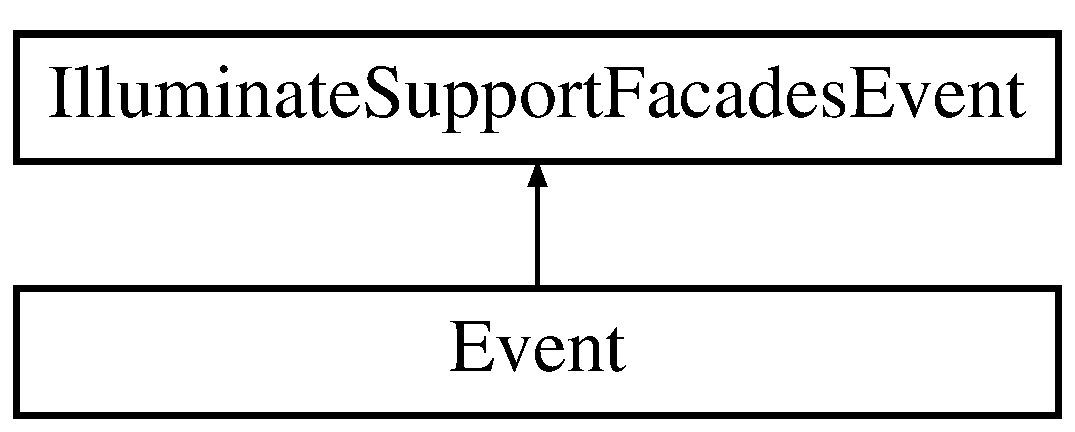
\includegraphics[height=2.000000cm]{class_event}
\end{center}
\end{figure}
\subsection*{Additional Inherited Members}


The documentation for this class was generated from the following file\+:\begin{DoxyCompactItemize}
\item 
\+\_\+ide\+\_\+helper.\+php\end{DoxyCompactItemize}

\hypertarget{class_illuminate_1_1_support_1_1_facades_1_1_event}{}\section{Illuminate\textbackslash{}Support\textbackslash{}Facades\textbackslash{}Event Class Reference}
\label{class_illuminate_1_1_support_1_1_facades_1_1_event}\index{Illuminate\textbackslash{}\+Support\textbackslash{}\+Facades\textbackslash{}\+Event@{Illuminate\textbackslash{}\+Support\textbackslash{}\+Facades\textbackslash{}\+Event}}
Inheritance diagram for Illuminate\textbackslash{}Support\textbackslash{}Facades\textbackslash{}Event\+:\begin{figure}[H]
\begin{center}
\leavevmode
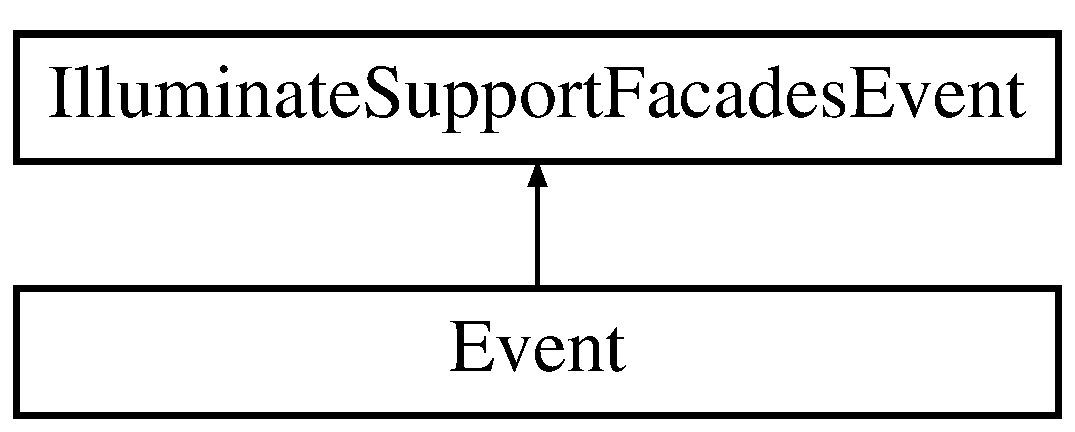
\includegraphics[height=2.000000cm]{class_illuminate_1_1_support_1_1_facades_1_1_event}
\end{center}
\end{figure}
\subsection*{Static Public Member Functions}
\begin{DoxyCompactItemize}
\item 
static \mbox{\hyperlink{class_illuminate_1_1_support_1_1_facades_1_1_event_af6c77b8d45f8a0388c29f575bfec20db}{listen}} (\$events, \$listener)
\item 
static \mbox{\hyperlink{class_illuminate_1_1_support_1_1_facades_1_1_event_af1445f8e4da4a24d97aec517d82923b9}{has\+Listeners}} (\$event\+Name)
\item 
static \mbox{\hyperlink{class_illuminate_1_1_support_1_1_facades_1_1_event_a92bcef26cffc44eaa728d5a42213b43c}{push}} (\$event, \$payload=array())
\item 
static \mbox{\hyperlink{class_illuminate_1_1_support_1_1_facades_1_1_event_ae092ef357ca1cb0e7acca1407529f94c}{flush}} (\$event)
\item 
static \mbox{\hyperlink{class_illuminate_1_1_support_1_1_facades_1_1_event_afe5054be218b0935bdf84281f57a8910}{subscribe}} (\$subscriber)
\item 
static \mbox{\hyperlink{class_illuminate_1_1_support_1_1_facades_1_1_event_aa040042f059fbe08c9b936276c70f9cc}{until}} (\$event, \$payload=array())
\item 
static \mbox{\hyperlink{class_illuminate_1_1_support_1_1_facades_1_1_event_a44e799906c5fc88d04fb7859d6a42641}{fire}} (\$event, \$payload=array(), \$halt=false)
\item 
static \mbox{\hyperlink{class_illuminate_1_1_support_1_1_facades_1_1_event_a8807dbfc639e38325c8efbc58bcf97cc}{dispatch}} (\$event, \$payload=array(), \$halt=false)
\item 
static \mbox{\hyperlink{class_illuminate_1_1_support_1_1_facades_1_1_event_a03cc35afaa8327ba99604171c312198e}{get\+Listeners}} (\$event\+Name)
\item 
static \mbox{\hyperlink{class_illuminate_1_1_support_1_1_facades_1_1_event_a6264ee9533ccc8443b4a892979ad1211}{make\+Listener}} (\$listener, \$wildcard=false)
\item 
static \mbox{\hyperlink{class_illuminate_1_1_support_1_1_facades_1_1_event_a1339e5e820a8d509e50d6787fb145c54}{create\+Class\+Listener}} (\$listener, \$wildcard=false)
\item 
static \mbox{\hyperlink{class_illuminate_1_1_support_1_1_facades_1_1_event_a34e852aad1b68390255dcdb664fcdf13}{forget}} (\$event)
\item 
static \mbox{\hyperlink{class_illuminate_1_1_support_1_1_facades_1_1_event_ad1e8988ddbc72a930b91bb9e30b15c6e}{forget\+Pushed}} ()
\item 
static \mbox{\hyperlink{class_illuminate_1_1_support_1_1_facades_1_1_event_af335a488b7fd410572a91b3e60efde50}{set\+Queue\+Resolver}} (\$resolver)
\end{DoxyCompactItemize}


\subsection{Member Function Documentation}
\mbox{\Hypertarget{class_illuminate_1_1_support_1_1_facades_1_1_event_a1339e5e820a8d509e50d6787fb145c54}\label{class_illuminate_1_1_support_1_1_facades_1_1_event_a1339e5e820a8d509e50d6787fb145c54}} 
\index{Illuminate\+::\+Support\+::\+Facades\+::\+Event@{Illuminate\+::\+Support\+::\+Facades\+::\+Event}!create\+Class\+Listener@{create\+Class\+Listener}}
\index{create\+Class\+Listener@{create\+Class\+Listener}!Illuminate\+::\+Support\+::\+Facades\+::\+Event@{Illuminate\+::\+Support\+::\+Facades\+::\+Event}}
\subsubsection{\texorpdfstring{create\+Class\+Listener()}{createClassListener()}}
{\footnotesize\ttfamily static Illuminate\textbackslash{}\+Support\textbackslash{}\+Facades\textbackslash{}\+Event\+::create\+Class\+Listener (\begin{DoxyParamCaption}\item[{}]{\$listener,  }\item[{}]{\$wildcard = {\ttfamily false} }\end{DoxyParamCaption})\hspace{0.3cm}{\ttfamily [static]}}

Create a class based listener using the IoC container.


\begin{DoxyParams}[1]{Parameters}
string & {\em \$listener} & \\
\hline
bool & {\em \$wildcard} & \\
\hline
\end{DoxyParams}
\begin{DoxyReturn}{Returns}

\end{DoxyReturn}
\mbox{\Hypertarget{class_illuminate_1_1_support_1_1_facades_1_1_event_a8807dbfc639e38325c8efbc58bcf97cc}\label{class_illuminate_1_1_support_1_1_facades_1_1_event_a8807dbfc639e38325c8efbc58bcf97cc}} 
\index{Illuminate\+::\+Support\+::\+Facades\+::\+Event@{Illuminate\+::\+Support\+::\+Facades\+::\+Event}!dispatch@{dispatch}}
\index{dispatch@{dispatch}!Illuminate\+::\+Support\+::\+Facades\+::\+Event@{Illuminate\+::\+Support\+::\+Facades\+::\+Event}}
\subsubsection{\texorpdfstring{dispatch()}{dispatch()}}
{\footnotesize\ttfamily static Illuminate\textbackslash{}\+Support\textbackslash{}\+Facades\textbackslash{}\+Event\+::dispatch (\begin{DoxyParamCaption}\item[{}]{\$event,  }\item[{}]{\$payload = {\ttfamily array()},  }\item[{}]{\$halt = {\ttfamily false} }\end{DoxyParamCaption})\hspace{0.3cm}{\ttfamily [static]}}

Fire an event and call the listeners.


\begin{DoxyParams}[1]{Parameters}
string | object & {\em \$event} & \\
\hline
mixed & {\em \$payload} & \\
\hline
bool & {\em \$halt} & \\
\hline
\end{DoxyParams}
\begin{DoxyReturn}{Returns}
array$\vert$null 
\end{DoxyReturn}
\mbox{\Hypertarget{class_illuminate_1_1_support_1_1_facades_1_1_event_a44e799906c5fc88d04fb7859d6a42641}\label{class_illuminate_1_1_support_1_1_facades_1_1_event_a44e799906c5fc88d04fb7859d6a42641}} 
\index{Illuminate\+::\+Support\+::\+Facades\+::\+Event@{Illuminate\+::\+Support\+::\+Facades\+::\+Event}!fire@{fire}}
\index{fire@{fire}!Illuminate\+::\+Support\+::\+Facades\+::\+Event@{Illuminate\+::\+Support\+::\+Facades\+::\+Event}}
\subsubsection{\texorpdfstring{fire()}{fire()}}
{\footnotesize\ttfamily static Illuminate\textbackslash{}\+Support\textbackslash{}\+Facades\textbackslash{}\+Event\+::fire (\begin{DoxyParamCaption}\item[{}]{\$event,  }\item[{}]{\$payload = {\ttfamily array()},  }\item[{}]{\$halt = {\ttfamily false} }\end{DoxyParamCaption})\hspace{0.3cm}{\ttfamily [static]}}

Fire an event and call the listeners.


\begin{DoxyParams}[1]{Parameters}
string | object & {\em \$event} & \\
\hline
mixed & {\em \$payload} & \\
\hline
bool & {\em \$halt} & \\
\hline
\end{DoxyParams}
\begin{DoxyReturn}{Returns}
array$\vert$null 
\end{DoxyReturn}
\mbox{\Hypertarget{class_illuminate_1_1_support_1_1_facades_1_1_event_ae092ef357ca1cb0e7acca1407529f94c}\label{class_illuminate_1_1_support_1_1_facades_1_1_event_ae092ef357ca1cb0e7acca1407529f94c}} 
\index{Illuminate\+::\+Support\+::\+Facades\+::\+Event@{Illuminate\+::\+Support\+::\+Facades\+::\+Event}!flush@{flush}}
\index{flush@{flush}!Illuminate\+::\+Support\+::\+Facades\+::\+Event@{Illuminate\+::\+Support\+::\+Facades\+::\+Event}}
\subsubsection{\texorpdfstring{flush()}{flush()}}
{\footnotesize\ttfamily static Illuminate\textbackslash{}\+Support\textbackslash{}\+Facades\textbackslash{}\+Event\+::flush (\begin{DoxyParamCaption}\item[{}]{\$event }\end{DoxyParamCaption})\hspace{0.3cm}{\ttfamily [static]}}

Flush a set of pushed events.


\begin{DoxyParams}[1]{Parameters}
string & {\em \$event} & \\
\hline
\end{DoxyParams}
\begin{DoxyReturn}{Returns}
void 
\end{DoxyReturn}
\mbox{\Hypertarget{class_illuminate_1_1_support_1_1_facades_1_1_event_a34e852aad1b68390255dcdb664fcdf13}\label{class_illuminate_1_1_support_1_1_facades_1_1_event_a34e852aad1b68390255dcdb664fcdf13}} 
\index{Illuminate\+::\+Support\+::\+Facades\+::\+Event@{Illuminate\+::\+Support\+::\+Facades\+::\+Event}!forget@{forget}}
\index{forget@{forget}!Illuminate\+::\+Support\+::\+Facades\+::\+Event@{Illuminate\+::\+Support\+::\+Facades\+::\+Event}}
\subsubsection{\texorpdfstring{forget()}{forget()}}
{\footnotesize\ttfamily static Illuminate\textbackslash{}\+Support\textbackslash{}\+Facades\textbackslash{}\+Event\+::forget (\begin{DoxyParamCaption}\item[{}]{\$event }\end{DoxyParamCaption})\hspace{0.3cm}{\ttfamily [static]}}

Remove a set of listeners from the dispatcher.


\begin{DoxyParams}[1]{Parameters}
string & {\em \$event} & \\
\hline
\end{DoxyParams}
\begin{DoxyReturn}{Returns}
void 
\end{DoxyReturn}
\mbox{\Hypertarget{class_illuminate_1_1_support_1_1_facades_1_1_event_ad1e8988ddbc72a930b91bb9e30b15c6e}\label{class_illuminate_1_1_support_1_1_facades_1_1_event_ad1e8988ddbc72a930b91bb9e30b15c6e}} 
\index{Illuminate\+::\+Support\+::\+Facades\+::\+Event@{Illuminate\+::\+Support\+::\+Facades\+::\+Event}!forget\+Pushed@{forget\+Pushed}}
\index{forget\+Pushed@{forget\+Pushed}!Illuminate\+::\+Support\+::\+Facades\+::\+Event@{Illuminate\+::\+Support\+::\+Facades\+::\+Event}}
\subsubsection{\texorpdfstring{forget\+Pushed()}{forgetPushed()}}
{\footnotesize\ttfamily static Illuminate\textbackslash{}\+Support\textbackslash{}\+Facades\textbackslash{}\+Event\+::forget\+Pushed (\begin{DoxyParamCaption}{ }\end{DoxyParamCaption})\hspace{0.3cm}{\ttfamily [static]}}

Forget all of the pushed listeners.

\begin{DoxyReturn}{Returns}
void 
\end{DoxyReturn}
\mbox{\Hypertarget{class_illuminate_1_1_support_1_1_facades_1_1_event_a03cc35afaa8327ba99604171c312198e}\label{class_illuminate_1_1_support_1_1_facades_1_1_event_a03cc35afaa8327ba99604171c312198e}} 
\index{Illuminate\+::\+Support\+::\+Facades\+::\+Event@{Illuminate\+::\+Support\+::\+Facades\+::\+Event}!get\+Listeners@{get\+Listeners}}
\index{get\+Listeners@{get\+Listeners}!Illuminate\+::\+Support\+::\+Facades\+::\+Event@{Illuminate\+::\+Support\+::\+Facades\+::\+Event}}
\subsubsection{\texorpdfstring{get\+Listeners()}{getListeners()}}
{\footnotesize\ttfamily static Illuminate\textbackslash{}\+Support\textbackslash{}\+Facades\textbackslash{}\+Event\+::get\+Listeners (\begin{DoxyParamCaption}\item[{}]{\$event\+Name }\end{DoxyParamCaption})\hspace{0.3cm}{\ttfamily [static]}}

Get all of the listeners for a given event name.


\begin{DoxyParams}[1]{Parameters}
string & {\em \$event\+Name} & \\
\hline
\end{DoxyParams}
\begin{DoxyReturn}{Returns}
array 
\end{DoxyReturn}
\mbox{\Hypertarget{class_illuminate_1_1_support_1_1_facades_1_1_event_af1445f8e4da4a24d97aec517d82923b9}\label{class_illuminate_1_1_support_1_1_facades_1_1_event_af1445f8e4da4a24d97aec517d82923b9}} 
\index{Illuminate\+::\+Support\+::\+Facades\+::\+Event@{Illuminate\+::\+Support\+::\+Facades\+::\+Event}!has\+Listeners@{has\+Listeners}}
\index{has\+Listeners@{has\+Listeners}!Illuminate\+::\+Support\+::\+Facades\+::\+Event@{Illuminate\+::\+Support\+::\+Facades\+::\+Event}}
\subsubsection{\texorpdfstring{has\+Listeners()}{hasListeners()}}
{\footnotesize\ttfamily static Illuminate\textbackslash{}\+Support\textbackslash{}\+Facades\textbackslash{}\+Event\+::has\+Listeners (\begin{DoxyParamCaption}\item[{}]{\$event\+Name }\end{DoxyParamCaption})\hspace{0.3cm}{\ttfamily [static]}}

Determine if a given event has listeners.


\begin{DoxyParams}[1]{Parameters}
string & {\em \$event\+Name} & \\
\hline
\end{DoxyParams}
\begin{DoxyReturn}{Returns}
bool 
\end{DoxyReturn}
\mbox{\Hypertarget{class_illuminate_1_1_support_1_1_facades_1_1_event_af6c77b8d45f8a0388c29f575bfec20db}\label{class_illuminate_1_1_support_1_1_facades_1_1_event_af6c77b8d45f8a0388c29f575bfec20db}} 
\index{Illuminate\+::\+Support\+::\+Facades\+::\+Event@{Illuminate\+::\+Support\+::\+Facades\+::\+Event}!listen@{listen}}
\index{listen@{listen}!Illuminate\+::\+Support\+::\+Facades\+::\+Event@{Illuminate\+::\+Support\+::\+Facades\+::\+Event}}
\subsubsection{\texorpdfstring{listen()}{listen()}}
{\footnotesize\ttfamily static Illuminate\textbackslash{}\+Support\textbackslash{}\+Facades\textbackslash{}\+Event\+::listen (\begin{DoxyParamCaption}\item[{}]{\$events,  }\item[{}]{\$listener }\end{DoxyParamCaption})\hspace{0.3cm}{\ttfamily [static]}}

Register an event listener with the dispatcher.


\begin{DoxyParams}[1]{Parameters}
string | array & {\em \$events} & \\
\hline
mixed & {\em \$listener} & \\
\hline
\end{DoxyParams}
\begin{DoxyReturn}{Returns}
void 
\end{DoxyReturn}
\mbox{\Hypertarget{class_illuminate_1_1_support_1_1_facades_1_1_event_a6264ee9533ccc8443b4a892979ad1211}\label{class_illuminate_1_1_support_1_1_facades_1_1_event_a6264ee9533ccc8443b4a892979ad1211}} 
\index{Illuminate\+::\+Support\+::\+Facades\+::\+Event@{Illuminate\+::\+Support\+::\+Facades\+::\+Event}!make\+Listener@{make\+Listener}}
\index{make\+Listener@{make\+Listener}!Illuminate\+::\+Support\+::\+Facades\+::\+Event@{Illuminate\+::\+Support\+::\+Facades\+::\+Event}}
\subsubsection{\texorpdfstring{make\+Listener()}{makeListener()}}
{\footnotesize\ttfamily static Illuminate\textbackslash{}\+Support\textbackslash{}\+Facades\textbackslash{}\+Event\+::make\+Listener (\begin{DoxyParamCaption}\item[{}]{\$listener,  }\item[{}]{\$wildcard = {\ttfamily false} }\end{DoxyParamCaption})\hspace{0.3cm}{\ttfamily [static]}}

Register an event listener with the dispatcher.


\begin{DoxyParams}[1]{Parameters}
\textbackslash{}\+Closure | string & {\em \$listener} & \\
\hline
bool & {\em \$wildcard} & \\
\hline
\end{DoxyParams}
\begin{DoxyReturn}{Returns}

\end{DoxyReturn}
\mbox{\Hypertarget{class_illuminate_1_1_support_1_1_facades_1_1_event_a92bcef26cffc44eaa728d5a42213b43c}\label{class_illuminate_1_1_support_1_1_facades_1_1_event_a92bcef26cffc44eaa728d5a42213b43c}} 
\index{Illuminate\+::\+Support\+::\+Facades\+::\+Event@{Illuminate\+::\+Support\+::\+Facades\+::\+Event}!push@{push}}
\index{push@{push}!Illuminate\+::\+Support\+::\+Facades\+::\+Event@{Illuminate\+::\+Support\+::\+Facades\+::\+Event}}
\subsubsection{\texorpdfstring{push()}{push()}}
{\footnotesize\ttfamily static Illuminate\textbackslash{}\+Support\textbackslash{}\+Facades\textbackslash{}\+Event\+::push (\begin{DoxyParamCaption}\item[{}]{\$event,  }\item[{}]{\$payload = {\ttfamily array()} }\end{DoxyParamCaption})\hspace{0.3cm}{\ttfamily [static]}}

Register an event and payload to be fired later.


\begin{DoxyParams}[1]{Parameters}
string & {\em \$event} & \\
\hline
array & {\em \$payload} & \\
\hline
\end{DoxyParams}
\begin{DoxyReturn}{Returns}
void 
\end{DoxyReturn}
\mbox{\Hypertarget{class_illuminate_1_1_support_1_1_facades_1_1_event_af335a488b7fd410572a91b3e60efde50}\label{class_illuminate_1_1_support_1_1_facades_1_1_event_af335a488b7fd410572a91b3e60efde50}} 
\index{Illuminate\+::\+Support\+::\+Facades\+::\+Event@{Illuminate\+::\+Support\+::\+Facades\+::\+Event}!set\+Queue\+Resolver@{set\+Queue\+Resolver}}
\index{set\+Queue\+Resolver@{set\+Queue\+Resolver}!Illuminate\+::\+Support\+::\+Facades\+::\+Event@{Illuminate\+::\+Support\+::\+Facades\+::\+Event}}
\subsubsection{\texorpdfstring{set\+Queue\+Resolver()}{setQueueResolver()}}
{\footnotesize\ttfamily static Illuminate\textbackslash{}\+Support\textbackslash{}\+Facades\textbackslash{}\+Event\+::set\+Queue\+Resolver (\begin{DoxyParamCaption}\item[{}]{\$resolver }\end{DoxyParamCaption})\hspace{0.3cm}{\ttfamily [static]}}

Set the queue resolver implementation.


\begin{DoxyParams}[1]{Parameters}
callable & {\em \$resolver} & \\
\hline
\end{DoxyParams}
\begin{DoxyReturn}{Returns}
\$this 
\end{DoxyReturn}
\mbox{\Hypertarget{class_illuminate_1_1_support_1_1_facades_1_1_event_afe5054be218b0935bdf84281f57a8910}\label{class_illuminate_1_1_support_1_1_facades_1_1_event_afe5054be218b0935bdf84281f57a8910}} 
\index{Illuminate\+::\+Support\+::\+Facades\+::\+Event@{Illuminate\+::\+Support\+::\+Facades\+::\+Event}!subscribe@{subscribe}}
\index{subscribe@{subscribe}!Illuminate\+::\+Support\+::\+Facades\+::\+Event@{Illuminate\+::\+Support\+::\+Facades\+::\+Event}}
\subsubsection{\texorpdfstring{subscribe()}{subscribe()}}
{\footnotesize\ttfamily static Illuminate\textbackslash{}\+Support\textbackslash{}\+Facades\textbackslash{}\+Event\+::subscribe (\begin{DoxyParamCaption}\item[{}]{\$subscriber }\end{DoxyParamCaption})\hspace{0.3cm}{\ttfamily [static]}}

Register an event subscriber with the dispatcher.


\begin{DoxyParams}[1]{Parameters}
object | string & {\em \$subscriber} & \\
\hline
\end{DoxyParams}
\begin{DoxyReturn}{Returns}
void 
\end{DoxyReturn}
\mbox{\Hypertarget{class_illuminate_1_1_support_1_1_facades_1_1_event_aa040042f059fbe08c9b936276c70f9cc}\label{class_illuminate_1_1_support_1_1_facades_1_1_event_aa040042f059fbe08c9b936276c70f9cc}} 
\index{Illuminate\+::\+Support\+::\+Facades\+::\+Event@{Illuminate\+::\+Support\+::\+Facades\+::\+Event}!until@{until}}
\index{until@{until}!Illuminate\+::\+Support\+::\+Facades\+::\+Event@{Illuminate\+::\+Support\+::\+Facades\+::\+Event}}
\subsubsection{\texorpdfstring{until()}{until()}}
{\footnotesize\ttfamily static Illuminate\textbackslash{}\+Support\textbackslash{}\+Facades\textbackslash{}\+Event\+::until (\begin{DoxyParamCaption}\item[{}]{\$event,  }\item[{}]{\$payload = {\ttfamily array()} }\end{DoxyParamCaption})\hspace{0.3cm}{\ttfamily [static]}}

Fire an event until the first non-\/null response is returned.


\begin{DoxyParams}[1]{Parameters}
string | object & {\em \$event} & \\
\hline
mixed & {\em \$payload} & \\
\hline
\end{DoxyParams}
\begin{DoxyReturn}{Returns}
array$\vert$null 
\end{DoxyReturn}


The documentation for this class was generated from the following file\+:\begin{DoxyCompactItemize}
\item 
\+\_\+ide\+\_\+helper.\+php\end{DoxyCompactItemize}

\hypertarget{class_file}{}\section{File Class Reference}
\label{class_file}\index{File@{File}}
Inheritance diagram for File\+:\begin{figure}[H]
\begin{center}
\leavevmode
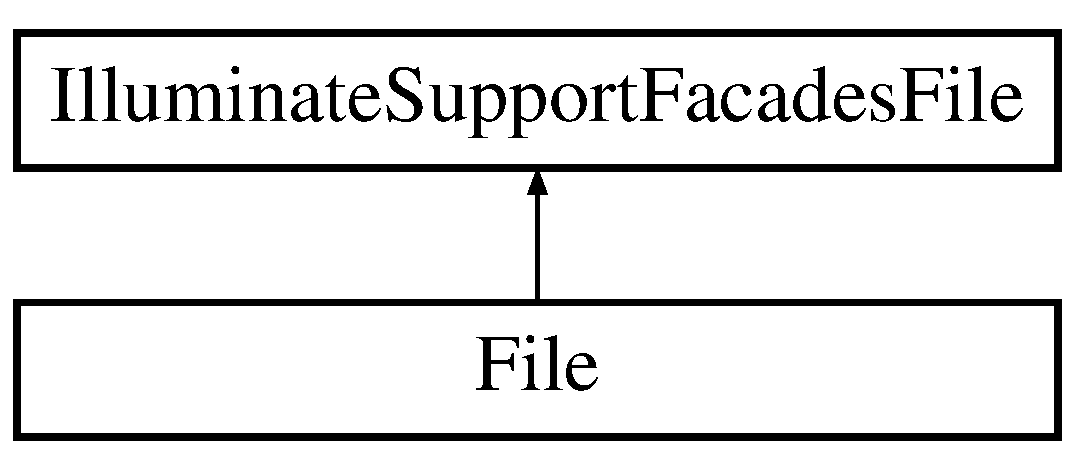
\includegraphics[height=2.000000cm]{class_file}
\end{center}
\end{figure}
\subsection*{Additional Inherited Members}


The documentation for this class was generated from the following file\+:\begin{DoxyCompactItemize}
\item 
\+\_\+ide\+\_\+helper.\+php\end{DoxyCompactItemize}

\hypertarget{class_illuminate_1_1_support_1_1_facades_1_1_file}{}\section{Illuminate\textbackslash{}Support\textbackslash{}Facades\textbackslash{}File Class Reference}
\label{class_illuminate_1_1_support_1_1_facades_1_1_file}\index{Illuminate\textbackslash{}\+Support\textbackslash{}\+Facades\textbackslash{}\+File@{Illuminate\textbackslash{}\+Support\textbackslash{}\+Facades\textbackslash{}\+File}}
Inheritance diagram for Illuminate\textbackslash{}Support\textbackslash{}Facades\textbackslash{}File\+:\begin{figure}[H]
\begin{center}
\leavevmode
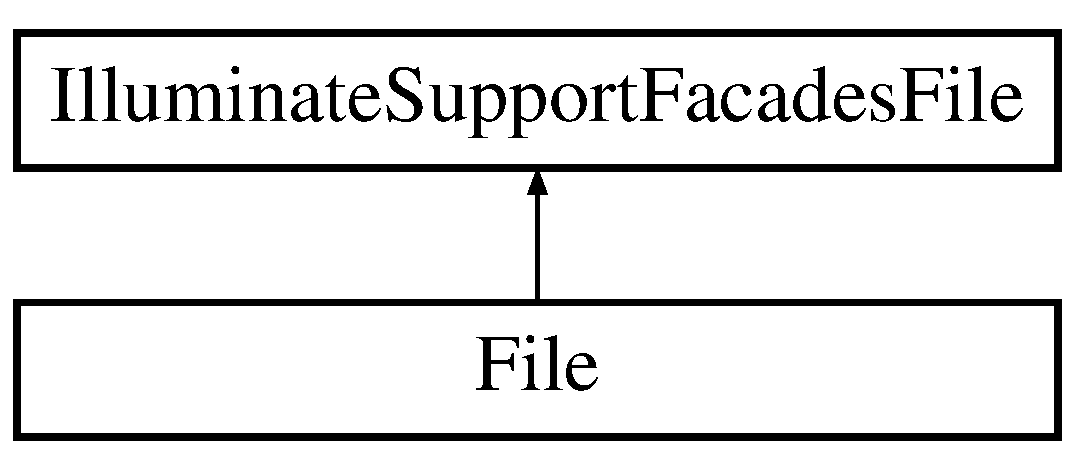
\includegraphics[height=2.000000cm]{class_illuminate_1_1_support_1_1_facades_1_1_file}
\end{center}
\end{figure}
\subsection*{Static Public Member Functions}
\begin{DoxyCompactItemize}
\item 
static \mbox{\hyperlink{class_illuminate_1_1_support_1_1_facades_1_1_file_a4b807c44b40f3f20c403e8bbed8b0a13}{exists}} (\$path)
\item 
static \mbox{\hyperlink{class_illuminate_1_1_support_1_1_facades_1_1_file_a4107d1371fced088f1d8cf9567462b2a}{get}} (\$path, \$lock=false)
\item 
static \mbox{\hyperlink{class_illuminate_1_1_support_1_1_facades_1_1_file_ae17d9ca36b3f2c31a3867bda05fd496d}{shared\+Get}} (\$path)
\item 
static \mbox{\hyperlink{class_illuminate_1_1_support_1_1_facades_1_1_file_a9d4a111e1e387d37a4dfdb3a2a1e551e}{get\+Require}} (\$path)
\item 
static \mbox{\hyperlink{class_illuminate_1_1_support_1_1_facades_1_1_file_a5f759ee620f8d2335fb6474bce2bae10}{require\+Once}} (\$file)
\item 
static \mbox{\hyperlink{class_illuminate_1_1_support_1_1_facades_1_1_file_a422b7ea35647d20d7d4937f0d30051dd}{hash}} (\$path)
\item 
static \mbox{\hyperlink{class_illuminate_1_1_support_1_1_facades_1_1_file_a3eecd0629a18f79867e78c128c3e8be4}{put}} (\$path, \$contents, \$lock=false)
\item 
static \mbox{\hyperlink{class_illuminate_1_1_support_1_1_facades_1_1_file_abb0f6b7ad9e25e7d4bab93b8452cd88a}{prepend}} (\$path, \$data)
\item 
static \mbox{\hyperlink{class_illuminate_1_1_support_1_1_facades_1_1_file_a7825529eea0804131cef0e9ae58b683d}{append}} (\$path, \$data)
\item 
static \mbox{\hyperlink{class_illuminate_1_1_support_1_1_facades_1_1_file_a8a69c6729054c846a7d524731c8c1401}{chmod}} (\$path, \$mode=null)
\item 
static \mbox{\hyperlink{class_illuminate_1_1_support_1_1_facades_1_1_file_ac679b60f28fd09f4489ed9c7f8864942}{delete}} (\$paths)
\item 
static \mbox{\hyperlink{class_illuminate_1_1_support_1_1_facades_1_1_file_afd1317f21e7e42c7e044422070ce9775}{move}} (\$path, \$target)
\item 
static \mbox{\hyperlink{class_illuminate_1_1_support_1_1_facades_1_1_file_a7f87dc02081585f2f2b3b6fe38d21c54}{copy}} (\$path, \$target)
\item 
static \mbox{\hyperlink{class_illuminate_1_1_support_1_1_facades_1_1_file_afe1409a45a5c4ad58f33f080a920044b}{link}} (\$target, \$link)
\item 
static \mbox{\hyperlink{class_illuminate_1_1_support_1_1_facades_1_1_file_a07e2149571901b2cb8ee8ed3804060f3}{name}} (\$path)
\item 
static \mbox{\hyperlink{class_illuminate_1_1_support_1_1_facades_1_1_file_a4292410fe2e9281cdf93724117954955}{basename}} (\$path)
\item 
static \mbox{\hyperlink{class_illuminate_1_1_support_1_1_facades_1_1_file_a59250be686860168cd5f0f5bad8c3aec}{dirname}} (\$path)
\item 
static \mbox{\hyperlink{class_illuminate_1_1_support_1_1_facades_1_1_file_a7fc0f3705cb3d6558796740a09d7c741}{extension}} (\$path)
\item 
static \mbox{\hyperlink{class_illuminate_1_1_support_1_1_facades_1_1_file_ab77fa1f772bbe857afb6f436af2aaf3f}{type}} (\$path)
\item 
static \mbox{\hyperlink{class_illuminate_1_1_support_1_1_facades_1_1_file_a23ad2113219fbb7b681bab6de6c36063}{mime\+Type}} (\$path)
\item 
static \mbox{\hyperlink{class_illuminate_1_1_support_1_1_facades_1_1_file_ae308662be3b972938b9060f5db95cee9}{size}} (\$path)
\item 
static \mbox{\hyperlink{class_illuminate_1_1_support_1_1_facades_1_1_file_a96eb9c1ffc4aabed4d270ac6eb3605d6}{last\+Modified}} (\$path)
\item 
static \mbox{\hyperlink{class_illuminate_1_1_support_1_1_facades_1_1_file_a3237a565dc6ae8c24f4b02e9ae5c3767}{is\+Directory}} (\$directory)
\item 
static \mbox{\hyperlink{class_illuminate_1_1_support_1_1_facades_1_1_file_a714920297a159ad88c60a875bdad6f8e}{is\+Readable}} (\$path)
\item 
static \mbox{\hyperlink{class_illuminate_1_1_support_1_1_facades_1_1_file_aca7ac18b51c114d25ac774b8d2b2324b}{is\+Writable}} (\$path)
\item 
static \mbox{\hyperlink{class_illuminate_1_1_support_1_1_facades_1_1_file_a7daf336670d1a9d836488e499eff44f6}{is\+File}} (\$file)
\item 
static \mbox{\hyperlink{class_illuminate_1_1_support_1_1_facades_1_1_file_af64ce811050d51d537898a17d493902f}{glob}} (\$pattern, \$flags=0)
\item 
static \mbox{\hyperlink{class_illuminate_1_1_support_1_1_facades_1_1_file_a014452088770b7b677cbe5543306f6c0}{files}} (\$directory, \$hidden=false)
\item 
static \mbox{\hyperlink{class_illuminate_1_1_support_1_1_facades_1_1_file_a1a1ef618cb8550450c2c9d2d0116677c}{all\+Files}} (\$directory, \$hidden=false)
\item 
static \mbox{\hyperlink{class_illuminate_1_1_support_1_1_facades_1_1_file_aa035c7fe1c5977b1ca3d709bf0c914a3}{directories}} (\$directory)
\item 
static \mbox{\hyperlink{class_illuminate_1_1_support_1_1_facades_1_1_file_a3eb1489a7e5c1489cf1168b662eebd1c}{make\+Directory}} (\$path, \$mode=493, \$recursive=false, \$force=false)
\item 
static \mbox{\hyperlink{class_illuminate_1_1_support_1_1_facades_1_1_file_a923b6ca0eaa520ba2030eab5e88cc917}{move\+Directory}} (\$from, \$to, \$overwrite=false)
\item 
static \mbox{\hyperlink{class_illuminate_1_1_support_1_1_facades_1_1_file_aa4b41b7c9242d5e1d12371733b00f9a3}{copy\+Directory}} (\$directory, \$destination, \$options=null)
\item 
static \mbox{\hyperlink{class_illuminate_1_1_support_1_1_facades_1_1_file_aa40074d950fe7b2f3f89a5c182b48aab}{delete\+Directory}} (\$directory, \$preserve=false)
\item 
static \mbox{\hyperlink{class_illuminate_1_1_support_1_1_facades_1_1_file_aa5d6dd162844e0bd915577ec06aedcc4}{clean\+Directory}} (\$directory)
\item 
static \mbox{\hyperlink{class_illuminate_1_1_support_1_1_facades_1_1_file_a577c40545aa409fb76915a39521db1cb}{macro}} (\$\mbox{\hyperlink{class_illuminate_1_1_support_1_1_facades_1_1_file_a07e2149571901b2cb8ee8ed3804060f3}{name}}, \$macro)
\item 
static \mbox{\hyperlink{class_illuminate_1_1_support_1_1_facades_1_1_file_a912083850797512cf5a62eaa3a39c3f0}{mixin}} (\$mixin)
\item 
static \mbox{\hyperlink{class_illuminate_1_1_support_1_1_facades_1_1_file_a6c644afd704f28fdaa3459e8c030b1e7}{has\+Macro}} (\$\mbox{\hyperlink{class_illuminate_1_1_support_1_1_facades_1_1_file_a07e2149571901b2cb8ee8ed3804060f3}{name}})
\end{DoxyCompactItemize}


\subsection{Member Function Documentation}
\mbox{\Hypertarget{class_illuminate_1_1_support_1_1_facades_1_1_file_a1a1ef618cb8550450c2c9d2d0116677c}\label{class_illuminate_1_1_support_1_1_facades_1_1_file_a1a1ef618cb8550450c2c9d2d0116677c}} 
\index{Illuminate\+::\+Support\+::\+Facades\+::\+File@{Illuminate\+::\+Support\+::\+Facades\+::\+File}!all\+Files@{all\+Files}}
\index{all\+Files@{all\+Files}!Illuminate\+::\+Support\+::\+Facades\+::\+File@{Illuminate\+::\+Support\+::\+Facades\+::\+File}}
\subsubsection{\texorpdfstring{all\+Files()}{allFiles()}}
{\footnotesize\ttfamily static Illuminate\textbackslash{}\+Support\textbackslash{}\+Facades\textbackslash{}\+File\+::all\+Files (\begin{DoxyParamCaption}\item[{}]{\$directory,  }\item[{}]{\$hidden = {\ttfamily false} }\end{DoxyParamCaption})\hspace{0.3cm}{\ttfamily [static]}}

Get all of the files from the given directory (recursive).


\begin{DoxyParams}[1]{Parameters}
string & {\em \$directory} & \\
\hline
bool & {\em \$hidden} & \\
\hline
\end{DoxyParams}
\begin{DoxyReturn}{Returns}
array 
\end{DoxyReturn}
\mbox{\Hypertarget{class_illuminate_1_1_support_1_1_facades_1_1_file_a7825529eea0804131cef0e9ae58b683d}\label{class_illuminate_1_1_support_1_1_facades_1_1_file_a7825529eea0804131cef0e9ae58b683d}} 
\index{Illuminate\+::\+Support\+::\+Facades\+::\+File@{Illuminate\+::\+Support\+::\+Facades\+::\+File}!append@{append}}
\index{append@{append}!Illuminate\+::\+Support\+::\+Facades\+::\+File@{Illuminate\+::\+Support\+::\+Facades\+::\+File}}
\subsubsection{\texorpdfstring{append()}{append()}}
{\footnotesize\ttfamily static Illuminate\textbackslash{}\+Support\textbackslash{}\+Facades\textbackslash{}\+File\+::append (\begin{DoxyParamCaption}\item[{}]{\$path,  }\item[{}]{\$data }\end{DoxyParamCaption})\hspace{0.3cm}{\ttfamily [static]}}

Append to a file.


\begin{DoxyParams}[1]{Parameters}
string & {\em \$path} & \\
\hline
string & {\em \$data} & \\
\hline
\end{DoxyParams}
\begin{DoxyReturn}{Returns}
int 
\end{DoxyReturn}
\mbox{\Hypertarget{class_illuminate_1_1_support_1_1_facades_1_1_file_a4292410fe2e9281cdf93724117954955}\label{class_illuminate_1_1_support_1_1_facades_1_1_file_a4292410fe2e9281cdf93724117954955}} 
\index{Illuminate\+::\+Support\+::\+Facades\+::\+File@{Illuminate\+::\+Support\+::\+Facades\+::\+File}!basename@{basename}}
\index{basename@{basename}!Illuminate\+::\+Support\+::\+Facades\+::\+File@{Illuminate\+::\+Support\+::\+Facades\+::\+File}}
\subsubsection{\texorpdfstring{basename()}{basename()}}
{\footnotesize\ttfamily static Illuminate\textbackslash{}\+Support\textbackslash{}\+Facades\textbackslash{}\+File\+::basename (\begin{DoxyParamCaption}\item[{}]{\$path }\end{DoxyParamCaption})\hspace{0.3cm}{\ttfamily [static]}}

Extract the trailing name component from a file path.


\begin{DoxyParams}[1]{Parameters}
string & {\em \$path} & \\
\hline
\end{DoxyParams}
\begin{DoxyReturn}{Returns}
string 
\end{DoxyReturn}
\mbox{\Hypertarget{class_illuminate_1_1_support_1_1_facades_1_1_file_a8a69c6729054c846a7d524731c8c1401}\label{class_illuminate_1_1_support_1_1_facades_1_1_file_a8a69c6729054c846a7d524731c8c1401}} 
\index{Illuminate\+::\+Support\+::\+Facades\+::\+File@{Illuminate\+::\+Support\+::\+Facades\+::\+File}!chmod@{chmod}}
\index{chmod@{chmod}!Illuminate\+::\+Support\+::\+Facades\+::\+File@{Illuminate\+::\+Support\+::\+Facades\+::\+File}}
\subsubsection{\texorpdfstring{chmod()}{chmod()}}
{\footnotesize\ttfamily static Illuminate\textbackslash{}\+Support\textbackslash{}\+Facades\textbackslash{}\+File\+::chmod (\begin{DoxyParamCaption}\item[{}]{\$path,  }\item[{}]{\$mode = {\ttfamily null} }\end{DoxyParamCaption})\hspace{0.3cm}{\ttfamily [static]}}

Get or set U\+N\+IX mode of a file or directory.


\begin{DoxyParams}[1]{Parameters}
string & {\em \$path} & \\
\hline
int & {\em \$mode} & \\
\hline
\end{DoxyParams}
\begin{DoxyReturn}{Returns}
mixed 
\end{DoxyReturn}
\mbox{\Hypertarget{class_illuminate_1_1_support_1_1_facades_1_1_file_aa5d6dd162844e0bd915577ec06aedcc4}\label{class_illuminate_1_1_support_1_1_facades_1_1_file_aa5d6dd162844e0bd915577ec06aedcc4}} 
\index{Illuminate\+::\+Support\+::\+Facades\+::\+File@{Illuminate\+::\+Support\+::\+Facades\+::\+File}!clean\+Directory@{clean\+Directory}}
\index{clean\+Directory@{clean\+Directory}!Illuminate\+::\+Support\+::\+Facades\+::\+File@{Illuminate\+::\+Support\+::\+Facades\+::\+File}}
\subsubsection{\texorpdfstring{clean\+Directory()}{cleanDirectory()}}
{\footnotesize\ttfamily static Illuminate\textbackslash{}\+Support\textbackslash{}\+Facades\textbackslash{}\+File\+::clean\+Directory (\begin{DoxyParamCaption}\item[{}]{\$directory }\end{DoxyParamCaption})\hspace{0.3cm}{\ttfamily [static]}}

Empty the specified directory of all files and folders.


\begin{DoxyParams}[1]{Parameters}
string & {\em \$directory} & \\
\hline
\end{DoxyParams}
\begin{DoxyReturn}{Returns}
bool 
\end{DoxyReturn}
\mbox{\Hypertarget{class_illuminate_1_1_support_1_1_facades_1_1_file_a7f87dc02081585f2f2b3b6fe38d21c54}\label{class_illuminate_1_1_support_1_1_facades_1_1_file_a7f87dc02081585f2f2b3b6fe38d21c54}} 
\index{Illuminate\+::\+Support\+::\+Facades\+::\+File@{Illuminate\+::\+Support\+::\+Facades\+::\+File}!copy@{copy}}
\index{copy@{copy}!Illuminate\+::\+Support\+::\+Facades\+::\+File@{Illuminate\+::\+Support\+::\+Facades\+::\+File}}
\subsubsection{\texorpdfstring{copy()}{copy()}}
{\footnotesize\ttfamily static Illuminate\textbackslash{}\+Support\textbackslash{}\+Facades\textbackslash{}\+File\+::copy (\begin{DoxyParamCaption}\item[{}]{\$path,  }\item[{}]{\$target }\end{DoxyParamCaption})\hspace{0.3cm}{\ttfamily [static]}}

Copy a file to a new location.


\begin{DoxyParams}[1]{Parameters}
string & {\em \$path} & \\
\hline
string & {\em \$target} & \\
\hline
\end{DoxyParams}
\begin{DoxyReturn}{Returns}
bool 
\end{DoxyReturn}
\mbox{\Hypertarget{class_illuminate_1_1_support_1_1_facades_1_1_file_aa4b41b7c9242d5e1d12371733b00f9a3}\label{class_illuminate_1_1_support_1_1_facades_1_1_file_aa4b41b7c9242d5e1d12371733b00f9a3}} 
\index{Illuminate\+::\+Support\+::\+Facades\+::\+File@{Illuminate\+::\+Support\+::\+Facades\+::\+File}!copy\+Directory@{copy\+Directory}}
\index{copy\+Directory@{copy\+Directory}!Illuminate\+::\+Support\+::\+Facades\+::\+File@{Illuminate\+::\+Support\+::\+Facades\+::\+File}}
\subsubsection{\texorpdfstring{copy\+Directory()}{copyDirectory()}}
{\footnotesize\ttfamily static Illuminate\textbackslash{}\+Support\textbackslash{}\+Facades\textbackslash{}\+File\+::copy\+Directory (\begin{DoxyParamCaption}\item[{}]{\$directory,  }\item[{}]{\$destination,  }\item[{}]{\$options = {\ttfamily null} }\end{DoxyParamCaption})\hspace{0.3cm}{\ttfamily [static]}}

Copy a directory from one location to another.


\begin{DoxyParams}[1]{Parameters}
string & {\em \$directory} & \\
\hline
string & {\em \$destination} & \\
\hline
int & {\em \$options} & \\
\hline
\end{DoxyParams}
\begin{DoxyReturn}{Returns}
bool 
\end{DoxyReturn}
\mbox{\Hypertarget{class_illuminate_1_1_support_1_1_facades_1_1_file_ac679b60f28fd09f4489ed9c7f8864942}\label{class_illuminate_1_1_support_1_1_facades_1_1_file_ac679b60f28fd09f4489ed9c7f8864942}} 
\index{Illuminate\+::\+Support\+::\+Facades\+::\+File@{Illuminate\+::\+Support\+::\+Facades\+::\+File}!delete@{delete}}
\index{delete@{delete}!Illuminate\+::\+Support\+::\+Facades\+::\+File@{Illuminate\+::\+Support\+::\+Facades\+::\+File}}
\subsubsection{\texorpdfstring{delete()}{delete()}}
{\footnotesize\ttfamily static Illuminate\textbackslash{}\+Support\textbackslash{}\+Facades\textbackslash{}\+File\+::delete (\begin{DoxyParamCaption}\item[{}]{\$paths }\end{DoxyParamCaption})\hspace{0.3cm}{\ttfamily [static]}}

Delete the file at a given path.


\begin{DoxyParams}[1]{Parameters}
string | array & {\em \$paths} & \\
\hline
\end{DoxyParams}
\begin{DoxyReturn}{Returns}
bool 
\end{DoxyReturn}
\mbox{\Hypertarget{class_illuminate_1_1_support_1_1_facades_1_1_file_aa40074d950fe7b2f3f89a5c182b48aab}\label{class_illuminate_1_1_support_1_1_facades_1_1_file_aa40074d950fe7b2f3f89a5c182b48aab}} 
\index{Illuminate\+::\+Support\+::\+Facades\+::\+File@{Illuminate\+::\+Support\+::\+Facades\+::\+File}!delete\+Directory@{delete\+Directory}}
\index{delete\+Directory@{delete\+Directory}!Illuminate\+::\+Support\+::\+Facades\+::\+File@{Illuminate\+::\+Support\+::\+Facades\+::\+File}}
\subsubsection{\texorpdfstring{delete\+Directory()}{deleteDirectory()}}
{\footnotesize\ttfamily static Illuminate\textbackslash{}\+Support\textbackslash{}\+Facades\textbackslash{}\+File\+::delete\+Directory (\begin{DoxyParamCaption}\item[{}]{\$directory,  }\item[{}]{\$preserve = {\ttfamily false} }\end{DoxyParamCaption})\hspace{0.3cm}{\ttfamily [static]}}

Recursively delete a directory.

The directory itself may be optionally preserved.


\begin{DoxyParams}[1]{Parameters}
string & {\em \$directory} & \\
\hline
bool & {\em \$preserve} & \\
\hline
\end{DoxyParams}
\begin{DoxyReturn}{Returns}
bool 
\end{DoxyReturn}
\mbox{\Hypertarget{class_illuminate_1_1_support_1_1_facades_1_1_file_aa035c7fe1c5977b1ca3d709bf0c914a3}\label{class_illuminate_1_1_support_1_1_facades_1_1_file_aa035c7fe1c5977b1ca3d709bf0c914a3}} 
\index{Illuminate\+::\+Support\+::\+Facades\+::\+File@{Illuminate\+::\+Support\+::\+Facades\+::\+File}!directories@{directories}}
\index{directories@{directories}!Illuminate\+::\+Support\+::\+Facades\+::\+File@{Illuminate\+::\+Support\+::\+Facades\+::\+File}}
\subsubsection{\texorpdfstring{directories()}{directories()}}
{\footnotesize\ttfamily static Illuminate\textbackslash{}\+Support\textbackslash{}\+Facades\textbackslash{}\+File\+::directories (\begin{DoxyParamCaption}\item[{}]{\$directory }\end{DoxyParamCaption})\hspace{0.3cm}{\ttfamily [static]}}

Get all of the directories within a given directory.


\begin{DoxyParams}[1]{Parameters}
string & {\em \$directory} & \\
\hline
\end{DoxyParams}
\begin{DoxyReturn}{Returns}
array 
\end{DoxyReturn}
\mbox{\Hypertarget{class_illuminate_1_1_support_1_1_facades_1_1_file_a59250be686860168cd5f0f5bad8c3aec}\label{class_illuminate_1_1_support_1_1_facades_1_1_file_a59250be686860168cd5f0f5bad8c3aec}} 
\index{Illuminate\+::\+Support\+::\+Facades\+::\+File@{Illuminate\+::\+Support\+::\+Facades\+::\+File}!dirname@{dirname}}
\index{dirname@{dirname}!Illuminate\+::\+Support\+::\+Facades\+::\+File@{Illuminate\+::\+Support\+::\+Facades\+::\+File}}
\subsubsection{\texorpdfstring{dirname()}{dirname()}}
{\footnotesize\ttfamily static Illuminate\textbackslash{}\+Support\textbackslash{}\+Facades\textbackslash{}\+File\+::dirname (\begin{DoxyParamCaption}\item[{}]{\$path }\end{DoxyParamCaption})\hspace{0.3cm}{\ttfamily [static]}}

Extract the parent directory from a file path.


\begin{DoxyParams}[1]{Parameters}
string & {\em \$path} & \\
\hline
\end{DoxyParams}
\begin{DoxyReturn}{Returns}
string 
\end{DoxyReturn}
\mbox{\Hypertarget{class_illuminate_1_1_support_1_1_facades_1_1_file_a4b807c44b40f3f20c403e8bbed8b0a13}\label{class_illuminate_1_1_support_1_1_facades_1_1_file_a4b807c44b40f3f20c403e8bbed8b0a13}} 
\index{Illuminate\+::\+Support\+::\+Facades\+::\+File@{Illuminate\+::\+Support\+::\+Facades\+::\+File}!exists@{exists}}
\index{exists@{exists}!Illuminate\+::\+Support\+::\+Facades\+::\+File@{Illuminate\+::\+Support\+::\+Facades\+::\+File}}
\subsubsection{\texorpdfstring{exists()}{exists()}}
{\footnotesize\ttfamily static Illuminate\textbackslash{}\+Support\textbackslash{}\+Facades\textbackslash{}\+File\+::exists (\begin{DoxyParamCaption}\item[{}]{\$path }\end{DoxyParamCaption})\hspace{0.3cm}{\ttfamily [static]}}

Determine if a file or directory exists.


\begin{DoxyParams}[1]{Parameters}
string & {\em \$path} & \\
\hline
\end{DoxyParams}
\begin{DoxyReturn}{Returns}
bool 
\end{DoxyReturn}
\mbox{\Hypertarget{class_illuminate_1_1_support_1_1_facades_1_1_file_a7fc0f3705cb3d6558796740a09d7c741}\label{class_illuminate_1_1_support_1_1_facades_1_1_file_a7fc0f3705cb3d6558796740a09d7c741}} 
\index{Illuminate\+::\+Support\+::\+Facades\+::\+File@{Illuminate\+::\+Support\+::\+Facades\+::\+File}!extension@{extension}}
\index{extension@{extension}!Illuminate\+::\+Support\+::\+Facades\+::\+File@{Illuminate\+::\+Support\+::\+Facades\+::\+File}}
\subsubsection{\texorpdfstring{extension()}{extension()}}
{\footnotesize\ttfamily static Illuminate\textbackslash{}\+Support\textbackslash{}\+Facades\textbackslash{}\+File\+::extension (\begin{DoxyParamCaption}\item[{}]{\$path }\end{DoxyParamCaption})\hspace{0.3cm}{\ttfamily [static]}}

Extract the file extension from a file path.


\begin{DoxyParams}[1]{Parameters}
string & {\em \$path} & \\
\hline
\end{DoxyParams}
\begin{DoxyReturn}{Returns}
string 
\end{DoxyReturn}
\mbox{\Hypertarget{class_illuminate_1_1_support_1_1_facades_1_1_file_a014452088770b7b677cbe5543306f6c0}\label{class_illuminate_1_1_support_1_1_facades_1_1_file_a014452088770b7b677cbe5543306f6c0}} 
\index{Illuminate\+::\+Support\+::\+Facades\+::\+File@{Illuminate\+::\+Support\+::\+Facades\+::\+File}!files@{files}}
\index{files@{files}!Illuminate\+::\+Support\+::\+Facades\+::\+File@{Illuminate\+::\+Support\+::\+Facades\+::\+File}}
\subsubsection{\texorpdfstring{files()}{files()}}
{\footnotesize\ttfamily static Illuminate\textbackslash{}\+Support\textbackslash{}\+Facades\textbackslash{}\+File\+::files (\begin{DoxyParamCaption}\item[{}]{\$directory,  }\item[{}]{\$hidden = {\ttfamily false} }\end{DoxyParamCaption})\hspace{0.3cm}{\ttfamily [static]}}

Get an array of all files in a directory.


\begin{DoxyParams}[1]{Parameters}
string & {\em \$directory} & \\
\hline
bool & {\em \$hidden} & \\
\hline
\end{DoxyParams}
\begin{DoxyReturn}{Returns}
array 
\end{DoxyReturn}
\mbox{\Hypertarget{class_illuminate_1_1_support_1_1_facades_1_1_file_a4107d1371fced088f1d8cf9567462b2a}\label{class_illuminate_1_1_support_1_1_facades_1_1_file_a4107d1371fced088f1d8cf9567462b2a}} 
\index{Illuminate\+::\+Support\+::\+Facades\+::\+File@{Illuminate\+::\+Support\+::\+Facades\+::\+File}!get@{get}}
\index{get@{get}!Illuminate\+::\+Support\+::\+Facades\+::\+File@{Illuminate\+::\+Support\+::\+Facades\+::\+File}}
\subsubsection{\texorpdfstring{get()}{get()}}
{\footnotesize\ttfamily static Illuminate\textbackslash{}\+Support\textbackslash{}\+Facades\textbackslash{}\+File\+::get (\begin{DoxyParamCaption}\item[{}]{\$path,  }\item[{}]{\$lock = {\ttfamily false} }\end{DoxyParamCaption})\hspace{0.3cm}{\ttfamily [static]}}

Get the contents of a file.


\begin{DoxyParams}[1]{Parameters}
string & {\em \$path} & \\
\hline
bool & {\em \$lock} & \\
\hline
\end{DoxyParams}
\begin{DoxyReturn}{Returns}
string 
\end{DoxyReturn}

\begin{DoxyExceptions}{Exceptions}
{\em } & \\
\hline
\end{DoxyExceptions}
\mbox{\Hypertarget{class_illuminate_1_1_support_1_1_facades_1_1_file_a9d4a111e1e387d37a4dfdb3a2a1e551e}\label{class_illuminate_1_1_support_1_1_facades_1_1_file_a9d4a111e1e387d37a4dfdb3a2a1e551e}} 
\index{Illuminate\+::\+Support\+::\+Facades\+::\+File@{Illuminate\+::\+Support\+::\+Facades\+::\+File}!get\+Require@{get\+Require}}
\index{get\+Require@{get\+Require}!Illuminate\+::\+Support\+::\+Facades\+::\+File@{Illuminate\+::\+Support\+::\+Facades\+::\+File}}
\subsubsection{\texorpdfstring{get\+Require()}{getRequire()}}
{\footnotesize\ttfamily static Illuminate\textbackslash{}\+Support\textbackslash{}\+Facades\textbackslash{}\+File\+::get\+Require (\begin{DoxyParamCaption}\item[{}]{\$path }\end{DoxyParamCaption})\hspace{0.3cm}{\ttfamily [static]}}

Get the returned value of a file.


\begin{DoxyParams}[1]{Parameters}
string & {\em \$path} & \\
\hline
\end{DoxyParams}
\begin{DoxyReturn}{Returns}
mixed 
\end{DoxyReturn}

\begin{DoxyExceptions}{Exceptions}
{\em } & \\
\hline
\end{DoxyExceptions}
\mbox{\Hypertarget{class_illuminate_1_1_support_1_1_facades_1_1_file_af64ce811050d51d537898a17d493902f}\label{class_illuminate_1_1_support_1_1_facades_1_1_file_af64ce811050d51d537898a17d493902f}} 
\index{Illuminate\+::\+Support\+::\+Facades\+::\+File@{Illuminate\+::\+Support\+::\+Facades\+::\+File}!glob@{glob}}
\index{glob@{glob}!Illuminate\+::\+Support\+::\+Facades\+::\+File@{Illuminate\+::\+Support\+::\+Facades\+::\+File}}
\subsubsection{\texorpdfstring{glob()}{glob()}}
{\footnotesize\ttfamily static Illuminate\textbackslash{}\+Support\textbackslash{}\+Facades\textbackslash{}\+File\+::glob (\begin{DoxyParamCaption}\item[{}]{\$pattern,  }\item[{}]{\$flags = {\ttfamily 0} }\end{DoxyParamCaption})\hspace{0.3cm}{\ttfamily [static]}}

Find path names matching a given pattern.


\begin{DoxyParams}[1]{Parameters}
string & {\em \$pattern} & \\
\hline
int & {\em \$flags} & \\
\hline
\end{DoxyParams}
\begin{DoxyReturn}{Returns}
array 
\end{DoxyReturn}
\mbox{\Hypertarget{class_illuminate_1_1_support_1_1_facades_1_1_file_a422b7ea35647d20d7d4937f0d30051dd}\label{class_illuminate_1_1_support_1_1_facades_1_1_file_a422b7ea35647d20d7d4937f0d30051dd}} 
\index{Illuminate\+::\+Support\+::\+Facades\+::\+File@{Illuminate\+::\+Support\+::\+Facades\+::\+File}!hash@{hash}}
\index{hash@{hash}!Illuminate\+::\+Support\+::\+Facades\+::\+File@{Illuminate\+::\+Support\+::\+Facades\+::\+File}}
\subsubsection{\texorpdfstring{hash()}{hash()}}
{\footnotesize\ttfamily static Illuminate\textbackslash{}\+Support\textbackslash{}\+Facades\textbackslash{}\+File\+::hash (\begin{DoxyParamCaption}\item[{}]{\$path }\end{DoxyParamCaption})\hspace{0.3cm}{\ttfamily [static]}}

Get the M\+D5 hash of the file at the given path.


\begin{DoxyParams}[1]{Parameters}
string & {\em \$path} & \\
\hline
\end{DoxyParams}
\begin{DoxyReturn}{Returns}
string 
\end{DoxyReturn}
\mbox{\Hypertarget{class_illuminate_1_1_support_1_1_facades_1_1_file_a6c644afd704f28fdaa3459e8c030b1e7}\label{class_illuminate_1_1_support_1_1_facades_1_1_file_a6c644afd704f28fdaa3459e8c030b1e7}} 
\index{Illuminate\+::\+Support\+::\+Facades\+::\+File@{Illuminate\+::\+Support\+::\+Facades\+::\+File}!has\+Macro@{has\+Macro}}
\index{has\+Macro@{has\+Macro}!Illuminate\+::\+Support\+::\+Facades\+::\+File@{Illuminate\+::\+Support\+::\+Facades\+::\+File}}
\subsubsection{\texorpdfstring{has\+Macro()}{hasMacro()}}
{\footnotesize\ttfamily static Illuminate\textbackslash{}\+Support\textbackslash{}\+Facades\textbackslash{}\+File\+::has\+Macro (\begin{DoxyParamCaption}\item[{}]{\$name }\end{DoxyParamCaption})\hspace{0.3cm}{\ttfamily [static]}}

Checks if macro is registered.


\begin{DoxyParams}[1]{Parameters}
string & {\em \$name} & \\
\hline
\end{DoxyParams}
\begin{DoxyReturn}{Returns}
bool 
\end{DoxyReturn}
\mbox{\Hypertarget{class_illuminate_1_1_support_1_1_facades_1_1_file_a3237a565dc6ae8c24f4b02e9ae5c3767}\label{class_illuminate_1_1_support_1_1_facades_1_1_file_a3237a565dc6ae8c24f4b02e9ae5c3767}} 
\index{Illuminate\+::\+Support\+::\+Facades\+::\+File@{Illuminate\+::\+Support\+::\+Facades\+::\+File}!is\+Directory@{is\+Directory}}
\index{is\+Directory@{is\+Directory}!Illuminate\+::\+Support\+::\+Facades\+::\+File@{Illuminate\+::\+Support\+::\+Facades\+::\+File}}
\subsubsection{\texorpdfstring{is\+Directory()}{isDirectory()}}
{\footnotesize\ttfamily static Illuminate\textbackslash{}\+Support\textbackslash{}\+Facades\textbackslash{}\+File\+::is\+Directory (\begin{DoxyParamCaption}\item[{}]{\$directory }\end{DoxyParamCaption})\hspace{0.3cm}{\ttfamily [static]}}

Determine if the given path is a directory.


\begin{DoxyParams}[1]{Parameters}
string & {\em \$directory} & \\
\hline
\end{DoxyParams}
\begin{DoxyReturn}{Returns}
bool 
\end{DoxyReturn}
\mbox{\Hypertarget{class_illuminate_1_1_support_1_1_facades_1_1_file_a7daf336670d1a9d836488e499eff44f6}\label{class_illuminate_1_1_support_1_1_facades_1_1_file_a7daf336670d1a9d836488e499eff44f6}} 
\index{Illuminate\+::\+Support\+::\+Facades\+::\+File@{Illuminate\+::\+Support\+::\+Facades\+::\+File}!is\+File@{is\+File}}
\index{is\+File@{is\+File}!Illuminate\+::\+Support\+::\+Facades\+::\+File@{Illuminate\+::\+Support\+::\+Facades\+::\+File}}
\subsubsection{\texorpdfstring{is\+File()}{isFile()}}
{\footnotesize\ttfamily static Illuminate\textbackslash{}\+Support\textbackslash{}\+Facades\textbackslash{}\+File\+::is\+File (\begin{DoxyParamCaption}\item[{}]{\$file }\end{DoxyParamCaption})\hspace{0.3cm}{\ttfamily [static]}}

Determine if the given path is a file.


\begin{DoxyParams}[1]{Parameters}
string & {\em \$file} & \\
\hline
\end{DoxyParams}
\begin{DoxyReturn}{Returns}
bool 
\end{DoxyReturn}
\mbox{\Hypertarget{class_illuminate_1_1_support_1_1_facades_1_1_file_a714920297a159ad88c60a875bdad6f8e}\label{class_illuminate_1_1_support_1_1_facades_1_1_file_a714920297a159ad88c60a875bdad6f8e}} 
\index{Illuminate\+::\+Support\+::\+Facades\+::\+File@{Illuminate\+::\+Support\+::\+Facades\+::\+File}!is\+Readable@{is\+Readable}}
\index{is\+Readable@{is\+Readable}!Illuminate\+::\+Support\+::\+Facades\+::\+File@{Illuminate\+::\+Support\+::\+Facades\+::\+File}}
\subsubsection{\texorpdfstring{is\+Readable()}{isReadable()}}
{\footnotesize\ttfamily static Illuminate\textbackslash{}\+Support\textbackslash{}\+Facades\textbackslash{}\+File\+::is\+Readable (\begin{DoxyParamCaption}\item[{}]{\$path }\end{DoxyParamCaption})\hspace{0.3cm}{\ttfamily [static]}}

Determine if the given path is readable.


\begin{DoxyParams}[1]{Parameters}
string & {\em \$path} & \\
\hline
\end{DoxyParams}
\begin{DoxyReturn}{Returns}
bool 
\end{DoxyReturn}
\mbox{\Hypertarget{class_illuminate_1_1_support_1_1_facades_1_1_file_aca7ac18b51c114d25ac774b8d2b2324b}\label{class_illuminate_1_1_support_1_1_facades_1_1_file_aca7ac18b51c114d25ac774b8d2b2324b}} 
\index{Illuminate\+::\+Support\+::\+Facades\+::\+File@{Illuminate\+::\+Support\+::\+Facades\+::\+File}!is\+Writable@{is\+Writable}}
\index{is\+Writable@{is\+Writable}!Illuminate\+::\+Support\+::\+Facades\+::\+File@{Illuminate\+::\+Support\+::\+Facades\+::\+File}}
\subsubsection{\texorpdfstring{is\+Writable()}{isWritable()}}
{\footnotesize\ttfamily static Illuminate\textbackslash{}\+Support\textbackslash{}\+Facades\textbackslash{}\+File\+::is\+Writable (\begin{DoxyParamCaption}\item[{}]{\$path }\end{DoxyParamCaption})\hspace{0.3cm}{\ttfamily [static]}}

Determine if the given path is writable.


\begin{DoxyParams}[1]{Parameters}
string & {\em \$path} & \\
\hline
\end{DoxyParams}
\begin{DoxyReturn}{Returns}
bool 
\end{DoxyReturn}
\mbox{\Hypertarget{class_illuminate_1_1_support_1_1_facades_1_1_file_a96eb9c1ffc4aabed4d270ac6eb3605d6}\label{class_illuminate_1_1_support_1_1_facades_1_1_file_a96eb9c1ffc4aabed4d270ac6eb3605d6}} 
\index{Illuminate\+::\+Support\+::\+Facades\+::\+File@{Illuminate\+::\+Support\+::\+Facades\+::\+File}!last\+Modified@{last\+Modified}}
\index{last\+Modified@{last\+Modified}!Illuminate\+::\+Support\+::\+Facades\+::\+File@{Illuminate\+::\+Support\+::\+Facades\+::\+File}}
\subsubsection{\texorpdfstring{last\+Modified()}{lastModified()}}
{\footnotesize\ttfamily static Illuminate\textbackslash{}\+Support\textbackslash{}\+Facades\textbackslash{}\+File\+::last\+Modified (\begin{DoxyParamCaption}\item[{}]{\$path }\end{DoxyParamCaption})\hspace{0.3cm}{\ttfamily [static]}}

Get the file\textquotesingle{}s last modification time.


\begin{DoxyParams}[1]{Parameters}
string & {\em \$path} & \\
\hline
\end{DoxyParams}
\begin{DoxyReturn}{Returns}
int 
\end{DoxyReturn}
\mbox{\Hypertarget{class_illuminate_1_1_support_1_1_facades_1_1_file_afe1409a45a5c4ad58f33f080a920044b}\label{class_illuminate_1_1_support_1_1_facades_1_1_file_afe1409a45a5c4ad58f33f080a920044b}} 
\index{Illuminate\+::\+Support\+::\+Facades\+::\+File@{Illuminate\+::\+Support\+::\+Facades\+::\+File}!link@{link}}
\index{link@{link}!Illuminate\+::\+Support\+::\+Facades\+::\+File@{Illuminate\+::\+Support\+::\+Facades\+::\+File}}
\subsubsection{\texorpdfstring{link()}{link()}}
{\footnotesize\ttfamily static Illuminate\textbackslash{}\+Support\textbackslash{}\+Facades\textbackslash{}\+File\+::link (\begin{DoxyParamCaption}\item[{}]{\$target,  }\item[{}]{\$link }\end{DoxyParamCaption})\hspace{0.3cm}{\ttfamily [static]}}

Create a hard link to the target file or directory.


\begin{DoxyParams}[1]{Parameters}
string & {\em \$target} & \\
\hline
string & {\em \$link} & \\
\hline
\end{DoxyParams}
\begin{DoxyReturn}{Returns}
void 
\end{DoxyReturn}
\mbox{\Hypertarget{class_illuminate_1_1_support_1_1_facades_1_1_file_a577c40545aa409fb76915a39521db1cb}\label{class_illuminate_1_1_support_1_1_facades_1_1_file_a577c40545aa409fb76915a39521db1cb}} 
\index{Illuminate\+::\+Support\+::\+Facades\+::\+File@{Illuminate\+::\+Support\+::\+Facades\+::\+File}!macro@{macro}}
\index{macro@{macro}!Illuminate\+::\+Support\+::\+Facades\+::\+File@{Illuminate\+::\+Support\+::\+Facades\+::\+File}}
\subsubsection{\texorpdfstring{macro()}{macro()}}
{\footnotesize\ttfamily static Illuminate\textbackslash{}\+Support\textbackslash{}\+Facades\textbackslash{}\+File\+::macro (\begin{DoxyParamCaption}\item[{}]{\$name,  }\item[{}]{\$macro }\end{DoxyParamCaption})\hspace{0.3cm}{\ttfamily [static]}}

Register a custom macro.


\begin{DoxyParams}[1]{Parameters}
string & {\em \$name} & \\
\hline
object | callable & {\em \$macro} & \\
\hline
\end{DoxyParams}
\begin{DoxyReturn}{Returns}
void 
\end{DoxyReturn}
\mbox{\Hypertarget{class_illuminate_1_1_support_1_1_facades_1_1_file_a3eb1489a7e5c1489cf1168b662eebd1c}\label{class_illuminate_1_1_support_1_1_facades_1_1_file_a3eb1489a7e5c1489cf1168b662eebd1c}} 
\index{Illuminate\+::\+Support\+::\+Facades\+::\+File@{Illuminate\+::\+Support\+::\+Facades\+::\+File}!make\+Directory@{make\+Directory}}
\index{make\+Directory@{make\+Directory}!Illuminate\+::\+Support\+::\+Facades\+::\+File@{Illuminate\+::\+Support\+::\+Facades\+::\+File}}
\subsubsection{\texorpdfstring{make\+Directory()}{makeDirectory()}}
{\footnotesize\ttfamily static Illuminate\textbackslash{}\+Support\textbackslash{}\+Facades\textbackslash{}\+File\+::make\+Directory (\begin{DoxyParamCaption}\item[{}]{\$path,  }\item[{}]{\$mode = {\ttfamily 493},  }\item[{}]{\$recursive = {\ttfamily false},  }\item[{}]{\$force = {\ttfamily false} }\end{DoxyParamCaption})\hspace{0.3cm}{\ttfamily [static]}}

Create a directory.


\begin{DoxyParams}[1]{Parameters}
string & {\em \$path} & \\
\hline
int & {\em \$mode} & \\
\hline
bool & {\em \$recursive} & \\
\hline
bool & {\em \$force} & \\
\hline
\end{DoxyParams}
\begin{DoxyReturn}{Returns}
bool 
\end{DoxyReturn}
\mbox{\Hypertarget{class_illuminate_1_1_support_1_1_facades_1_1_file_a23ad2113219fbb7b681bab6de6c36063}\label{class_illuminate_1_1_support_1_1_facades_1_1_file_a23ad2113219fbb7b681bab6de6c36063}} 
\index{Illuminate\+::\+Support\+::\+Facades\+::\+File@{Illuminate\+::\+Support\+::\+Facades\+::\+File}!mime\+Type@{mime\+Type}}
\index{mime\+Type@{mime\+Type}!Illuminate\+::\+Support\+::\+Facades\+::\+File@{Illuminate\+::\+Support\+::\+Facades\+::\+File}}
\subsubsection{\texorpdfstring{mime\+Type()}{mimeType()}}
{\footnotesize\ttfamily static Illuminate\textbackslash{}\+Support\textbackslash{}\+Facades\textbackslash{}\+File\+::mime\+Type (\begin{DoxyParamCaption}\item[{}]{\$path }\end{DoxyParamCaption})\hspace{0.3cm}{\ttfamily [static]}}

Get the mime-\/type of a given file.


\begin{DoxyParams}[1]{Parameters}
string & {\em \$path} & \\
\hline
\end{DoxyParams}
\begin{DoxyReturn}{Returns}
string$\vert$false 
\end{DoxyReturn}
\mbox{\Hypertarget{class_illuminate_1_1_support_1_1_facades_1_1_file_a912083850797512cf5a62eaa3a39c3f0}\label{class_illuminate_1_1_support_1_1_facades_1_1_file_a912083850797512cf5a62eaa3a39c3f0}} 
\index{Illuminate\+::\+Support\+::\+Facades\+::\+File@{Illuminate\+::\+Support\+::\+Facades\+::\+File}!mixin@{mixin}}
\index{mixin@{mixin}!Illuminate\+::\+Support\+::\+Facades\+::\+File@{Illuminate\+::\+Support\+::\+Facades\+::\+File}}
\subsubsection{\texorpdfstring{mixin()}{mixin()}}
{\footnotesize\ttfamily static Illuminate\textbackslash{}\+Support\textbackslash{}\+Facades\textbackslash{}\+File\+::mixin (\begin{DoxyParamCaption}\item[{}]{\$mixin }\end{DoxyParamCaption})\hspace{0.3cm}{\ttfamily [static]}}

Mix another object into the class.


\begin{DoxyParams}[1]{Parameters}
object & {\em \$mixin} & \\
\hline
\end{DoxyParams}
\begin{DoxyReturn}{Returns}
void 
\end{DoxyReturn}
\mbox{\Hypertarget{class_illuminate_1_1_support_1_1_facades_1_1_file_afd1317f21e7e42c7e044422070ce9775}\label{class_illuminate_1_1_support_1_1_facades_1_1_file_afd1317f21e7e42c7e044422070ce9775}} 
\index{Illuminate\+::\+Support\+::\+Facades\+::\+File@{Illuminate\+::\+Support\+::\+Facades\+::\+File}!move@{move}}
\index{move@{move}!Illuminate\+::\+Support\+::\+Facades\+::\+File@{Illuminate\+::\+Support\+::\+Facades\+::\+File}}
\subsubsection{\texorpdfstring{move()}{move()}}
{\footnotesize\ttfamily static Illuminate\textbackslash{}\+Support\textbackslash{}\+Facades\textbackslash{}\+File\+::move (\begin{DoxyParamCaption}\item[{}]{\$path,  }\item[{}]{\$target }\end{DoxyParamCaption})\hspace{0.3cm}{\ttfamily [static]}}

Move a file to a new location.


\begin{DoxyParams}[1]{Parameters}
string & {\em \$path} & \\
\hline
string & {\em \$target} & \\
\hline
\end{DoxyParams}
\begin{DoxyReturn}{Returns}
bool 
\end{DoxyReturn}
\mbox{\Hypertarget{class_illuminate_1_1_support_1_1_facades_1_1_file_a923b6ca0eaa520ba2030eab5e88cc917}\label{class_illuminate_1_1_support_1_1_facades_1_1_file_a923b6ca0eaa520ba2030eab5e88cc917}} 
\index{Illuminate\+::\+Support\+::\+Facades\+::\+File@{Illuminate\+::\+Support\+::\+Facades\+::\+File}!move\+Directory@{move\+Directory}}
\index{move\+Directory@{move\+Directory}!Illuminate\+::\+Support\+::\+Facades\+::\+File@{Illuminate\+::\+Support\+::\+Facades\+::\+File}}
\subsubsection{\texorpdfstring{move\+Directory()}{moveDirectory()}}
{\footnotesize\ttfamily static Illuminate\textbackslash{}\+Support\textbackslash{}\+Facades\textbackslash{}\+File\+::move\+Directory (\begin{DoxyParamCaption}\item[{}]{\$from,  }\item[{}]{\$to,  }\item[{}]{\$overwrite = {\ttfamily false} }\end{DoxyParamCaption})\hspace{0.3cm}{\ttfamily [static]}}

Move a directory.


\begin{DoxyParams}[1]{Parameters}
string & {\em \$from} & \\
\hline
string & {\em \$to} & \\
\hline
bool & {\em \$overwrite} & \\
\hline
\end{DoxyParams}
\begin{DoxyReturn}{Returns}
bool 
\end{DoxyReturn}
\mbox{\Hypertarget{class_illuminate_1_1_support_1_1_facades_1_1_file_a07e2149571901b2cb8ee8ed3804060f3}\label{class_illuminate_1_1_support_1_1_facades_1_1_file_a07e2149571901b2cb8ee8ed3804060f3}} 
\index{Illuminate\+::\+Support\+::\+Facades\+::\+File@{Illuminate\+::\+Support\+::\+Facades\+::\+File}!name@{name}}
\index{name@{name}!Illuminate\+::\+Support\+::\+Facades\+::\+File@{Illuminate\+::\+Support\+::\+Facades\+::\+File}}
\subsubsection{\texorpdfstring{name()}{name()}}
{\footnotesize\ttfamily static Illuminate\textbackslash{}\+Support\textbackslash{}\+Facades\textbackslash{}\+File\+::name (\begin{DoxyParamCaption}\item[{}]{\$path }\end{DoxyParamCaption})\hspace{0.3cm}{\ttfamily [static]}}

Extract the file name from a file path.


\begin{DoxyParams}[1]{Parameters}
string & {\em \$path} & \\
\hline
\end{DoxyParams}
\begin{DoxyReturn}{Returns}
string 
\end{DoxyReturn}
\mbox{\Hypertarget{class_illuminate_1_1_support_1_1_facades_1_1_file_abb0f6b7ad9e25e7d4bab93b8452cd88a}\label{class_illuminate_1_1_support_1_1_facades_1_1_file_abb0f6b7ad9e25e7d4bab93b8452cd88a}} 
\index{Illuminate\+::\+Support\+::\+Facades\+::\+File@{Illuminate\+::\+Support\+::\+Facades\+::\+File}!prepend@{prepend}}
\index{prepend@{prepend}!Illuminate\+::\+Support\+::\+Facades\+::\+File@{Illuminate\+::\+Support\+::\+Facades\+::\+File}}
\subsubsection{\texorpdfstring{prepend()}{prepend()}}
{\footnotesize\ttfamily static Illuminate\textbackslash{}\+Support\textbackslash{}\+Facades\textbackslash{}\+File\+::prepend (\begin{DoxyParamCaption}\item[{}]{\$path,  }\item[{}]{\$data }\end{DoxyParamCaption})\hspace{0.3cm}{\ttfamily [static]}}

Prepend to a file.


\begin{DoxyParams}[1]{Parameters}
string & {\em \$path} & \\
\hline
string & {\em \$data} & \\
\hline
\end{DoxyParams}
\begin{DoxyReturn}{Returns}
int 
\end{DoxyReturn}
\mbox{\Hypertarget{class_illuminate_1_1_support_1_1_facades_1_1_file_a3eecd0629a18f79867e78c128c3e8be4}\label{class_illuminate_1_1_support_1_1_facades_1_1_file_a3eecd0629a18f79867e78c128c3e8be4}} 
\index{Illuminate\+::\+Support\+::\+Facades\+::\+File@{Illuminate\+::\+Support\+::\+Facades\+::\+File}!put@{put}}
\index{put@{put}!Illuminate\+::\+Support\+::\+Facades\+::\+File@{Illuminate\+::\+Support\+::\+Facades\+::\+File}}
\subsubsection{\texorpdfstring{put()}{put()}}
{\footnotesize\ttfamily static Illuminate\textbackslash{}\+Support\textbackslash{}\+Facades\textbackslash{}\+File\+::put (\begin{DoxyParamCaption}\item[{}]{\$path,  }\item[{}]{\$contents,  }\item[{}]{\$lock = {\ttfamily false} }\end{DoxyParamCaption})\hspace{0.3cm}{\ttfamily [static]}}

Write the contents of a file.


\begin{DoxyParams}[1]{Parameters}
string & {\em \$path} & \\
\hline
string & {\em \$contents} & \\
\hline
bool & {\em \$lock} & \\
\hline
\end{DoxyParams}
\begin{DoxyReturn}{Returns}
int 
\end{DoxyReturn}
\mbox{\Hypertarget{class_illuminate_1_1_support_1_1_facades_1_1_file_a5f759ee620f8d2335fb6474bce2bae10}\label{class_illuminate_1_1_support_1_1_facades_1_1_file_a5f759ee620f8d2335fb6474bce2bae10}} 
\index{Illuminate\+::\+Support\+::\+Facades\+::\+File@{Illuminate\+::\+Support\+::\+Facades\+::\+File}!require\+Once@{require\+Once}}
\index{require\+Once@{require\+Once}!Illuminate\+::\+Support\+::\+Facades\+::\+File@{Illuminate\+::\+Support\+::\+Facades\+::\+File}}
\subsubsection{\texorpdfstring{require\+Once()}{requireOnce()}}
{\footnotesize\ttfamily static Illuminate\textbackslash{}\+Support\textbackslash{}\+Facades\textbackslash{}\+File\+::require\+Once (\begin{DoxyParamCaption}\item[{}]{\$file }\end{DoxyParamCaption})\hspace{0.3cm}{\ttfamily [static]}}

Require the given file once.


\begin{DoxyParams}[1]{Parameters}
string & {\em \$file} & \\
\hline
\end{DoxyParams}
\begin{DoxyReturn}{Returns}
mixed 
\end{DoxyReturn}
\mbox{\Hypertarget{class_illuminate_1_1_support_1_1_facades_1_1_file_ae17d9ca36b3f2c31a3867bda05fd496d}\label{class_illuminate_1_1_support_1_1_facades_1_1_file_ae17d9ca36b3f2c31a3867bda05fd496d}} 
\index{Illuminate\+::\+Support\+::\+Facades\+::\+File@{Illuminate\+::\+Support\+::\+Facades\+::\+File}!shared\+Get@{shared\+Get}}
\index{shared\+Get@{shared\+Get}!Illuminate\+::\+Support\+::\+Facades\+::\+File@{Illuminate\+::\+Support\+::\+Facades\+::\+File}}
\subsubsection{\texorpdfstring{shared\+Get()}{sharedGet()}}
{\footnotesize\ttfamily static Illuminate\textbackslash{}\+Support\textbackslash{}\+Facades\textbackslash{}\+File\+::shared\+Get (\begin{DoxyParamCaption}\item[{}]{\$path }\end{DoxyParamCaption})\hspace{0.3cm}{\ttfamily [static]}}

Get contents of a file with shared access.


\begin{DoxyParams}[1]{Parameters}
string & {\em \$path} & \\
\hline
\end{DoxyParams}
\begin{DoxyReturn}{Returns}
string 
\end{DoxyReturn}
\mbox{\Hypertarget{class_illuminate_1_1_support_1_1_facades_1_1_file_ae308662be3b972938b9060f5db95cee9}\label{class_illuminate_1_1_support_1_1_facades_1_1_file_ae308662be3b972938b9060f5db95cee9}} 
\index{Illuminate\+::\+Support\+::\+Facades\+::\+File@{Illuminate\+::\+Support\+::\+Facades\+::\+File}!size@{size}}
\index{size@{size}!Illuminate\+::\+Support\+::\+Facades\+::\+File@{Illuminate\+::\+Support\+::\+Facades\+::\+File}}
\subsubsection{\texorpdfstring{size()}{size()}}
{\footnotesize\ttfamily static Illuminate\textbackslash{}\+Support\textbackslash{}\+Facades\textbackslash{}\+File\+::size (\begin{DoxyParamCaption}\item[{}]{\$path }\end{DoxyParamCaption})\hspace{0.3cm}{\ttfamily [static]}}

Get the file size of a given file.


\begin{DoxyParams}[1]{Parameters}
string & {\em \$path} & \\
\hline
\end{DoxyParams}
\begin{DoxyReturn}{Returns}
int 
\end{DoxyReturn}
\mbox{\Hypertarget{class_illuminate_1_1_support_1_1_facades_1_1_file_ab77fa1f772bbe857afb6f436af2aaf3f}\label{class_illuminate_1_1_support_1_1_facades_1_1_file_ab77fa1f772bbe857afb6f436af2aaf3f}} 
\index{Illuminate\+::\+Support\+::\+Facades\+::\+File@{Illuminate\+::\+Support\+::\+Facades\+::\+File}!type@{type}}
\index{type@{type}!Illuminate\+::\+Support\+::\+Facades\+::\+File@{Illuminate\+::\+Support\+::\+Facades\+::\+File}}
\subsubsection{\texorpdfstring{type()}{type()}}
{\footnotesize\ttfamily static Illuminate\textbackslash{}\+Support\textbackslash{}\+Facades\textbackslash{}\+File\+::type (\begin{DoxyParamCaption}\item[{}]{\$path }\end{DoxyParamCaption})\hspace{0.3cm}{\ttfamily [static]}}

Get the file type of a given file.


\begin{DoxyParams}[1]{Parameters}
string & {\em \$path} & \\
\hline
\end{DoxyParams}
\begin{DoxyReturn}{Returns}
string 
\end{DoxyReturn}


The documentation for this class was generated from the following file\+:\begin{DoxyCompactItemize}
\item 
\+\_\+ide\+\_\+helper.\+php\end{DoxyCompactItemize}

\hypertarget{class_gate}{}\section{Gate Class Reference}
\label{class_gate}\index{Gate@{Gate}}
Inheritance diagram for Gate\+:\begin{figure}[H]
\begin{center}
\leavevmode
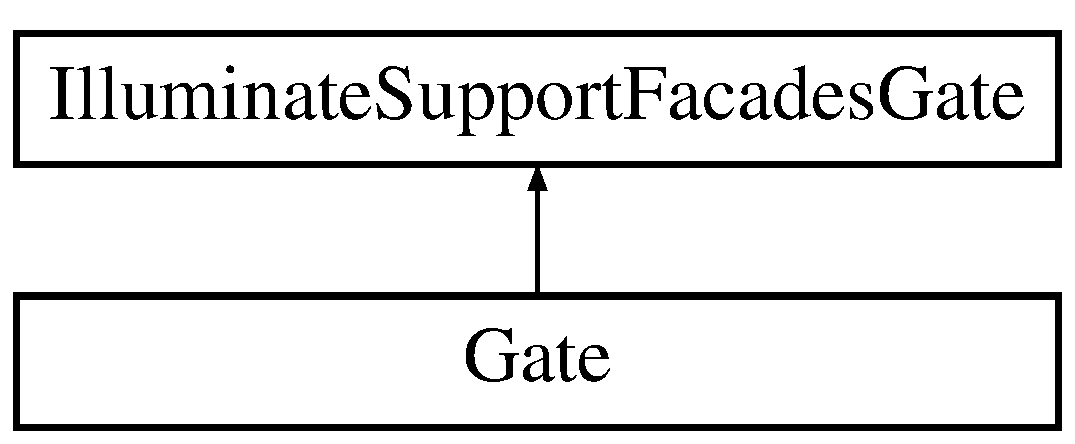
\includegraphics[height=2.000000cm]{class_gate}
\end{center}
\end{figure}
\subsection*{Additional Inherited Members}


The documentation for this class was generated from the following file\+:\begin{DoxyCompactItemize}
\item 
\+\_\+ide\+\_\+helper.\+php\end{DoxyCompactItemize}

\hypertarget{class_illuminate_1_1_support_1_1_facades_1_1_gate}{}\section{Illuminate\textbackslash{}Support\textbackslash{}Facades\textbackslash{}Gate Class Reference}
\label{class_illuminate_1_1_support_1_1_facades_1_1_gate}\index{Illuminate\textbackslash{}\+Support\textbackslash{}\+Facades\textbackslash{}\+Gate@{Illuminate\textbackslash{}\+Support\textbackslash{}\+Facades\textbackslash{}\+Gate}}
Inheritance diagram for Illuminate\textbackslash{}Support\textbackslash{}Facades\textbackslash{}Gate\+:\begin{figure}[H]
\begin{center}
\leavevmode
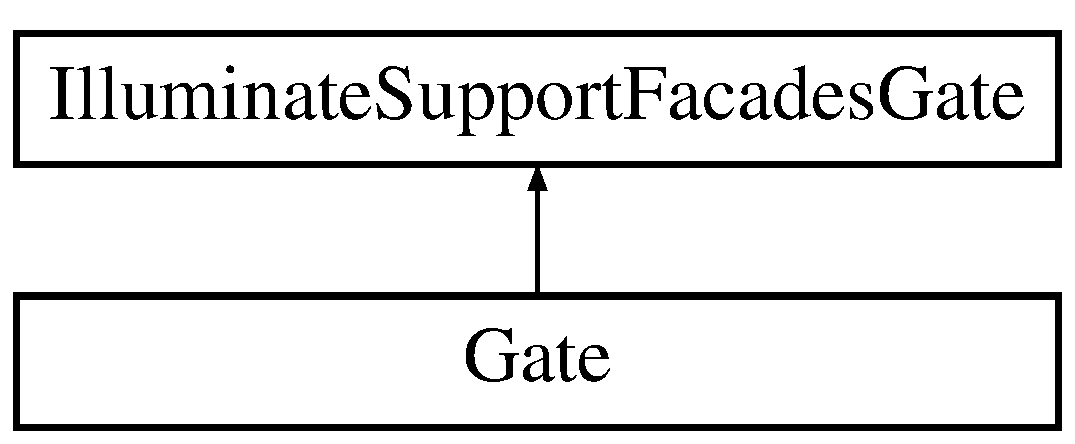
\includegraphics[height=2.000000cm]{class_illuminate_1_1_support_1_1_facades_1_1_gate}
\end{center}
\end{figure}
\subsection*{Static Public Member Functions}
\begin{DoxyCompactItemize}
\item 
static \mbox{\hyperlink{class_illuminate_1_1_support_1_1_facades_1_1_gate_a707cb199ec72119e5b85c25ad235004e}{has}} (\$ability)
\item 
static \mbox{\hyperlink{class_illuminate_1_1_support_1_1_facades_1_1_gate_af7f90f854ea9d7ce6c6d4a7665caeed4}{define}} (\$ability, \$callback)
\item 
static \mbox{\hyperlink{class_illuminate_1_1_support_1_1_facades_1_1_gate_a291645da3113160b150c1aec559cc28e}{resource}} (\$name, \$class, \$\mbox{\hyperlink{class_illuminate_1_1_support_1_1_facades_1_1_gate_ae4c194dfa7fc3157b19cfdd34a9eb989}{abilities}}=null)
\item 
static \mbox{\hyperlink{class_illuminate_1_1_support_1_1_facades_1_1_gate_ac9b97caa9e0f2149bf81706cffaaa49d}{policy}} (\$class, \$policy)
\item 
static \mbox{\hyperlink{class_illuminate_1_1_support_1_1_facades_1_1_gate_ac81a01d99657d6fc1e10dfff4faec994}{before}} (\$callback)
\item 
static \mbox{\hyperlink{class_illuminate_1_1_support_1_1_facades_1_1_gate_a18080477d595d620db9332f9d829503a}{after}} (\$callback)
\item 
static \mbox{\hyperlink{class_illuminate_1_1_support_1_1_facades_1_1_gate_acb9d26a32e44d841b4a374dc0aba8fb4}{allows}} (\$ability, \$arguments=array())
\item 
static \mbox{\hyperlink{class_illuminate_1_1_support_1_1_facades_1_1_gate_af5f76847d390f8c4d1092bee4a916f8e}{denies}} (\$ability, \$arguments=array())
\item 
static \mbox{\hyperlink{class_illuminate_1_1_support_1_1_facades_1_1_gate_ac4825419bb8e7a48b4ba1542f93ee3eb}{check}} (\$\mbox{\hyperlink{class_illuminate_1_1_support_1_1_facades_1_1_gate_ae4c194dfa7fc3157b19cfdd34a9eb989}{abilities}}, \$arguments=array())
\item 
static \mbox{\hyperlink{class_illuminate_1_1_support_1_1_facades_1_1_gate_a2527f977b0a27705cdd3b3300ae172bb}{any}} (\$\mbox{\hyperlink{class_illuminate_1_1_support_1_1_facades_1_1_gate_ae4c194dfa7fc3157b19cfdd34a9eb989}{abilities}}, \$arguments=array())
\item 
static \mbox{\hyperlink{class_illuminate_1_1_support_1_1_facades_1_1_gate_aa235db9683cd7d125fbd65a666172758}{authorize}} (\$ability, \$arguments=array())
\item 
static \mbox{\hyperlink{class_illuminate_1_1_support_1_1_facades_1_1_gate_a7c55d413c035d9f7c98f1c232af55b0a}{get\+Policy\+For}} (\$class)
\item 
static \mbox{\hyperlink{class_illuminate_1_1_support_1_1_facades_1_1_gate_a542f4d3d4a305070120eff8cd3740a2b}{resolve\+Policy}} (\$class)
\item 
static \mbox{\hyperlink{class_illuminate_1_1_support_1_1_facades_1_1_gate_a0dfe7611e3fa83b7964a15b2995c8771}{for\+User}} (\$user)
\item 
static \mbox{\hyperlink{class_illuminate_1_1_support_1_1_facades_1_1_gate_ae4c194dfa7fc3157b19cfdd34a9eb989}{abilities}} ()
\item 
static \mbox{\hyperlink{class_illuminate_1_1_support_1_1_facades_1_1_gate_a2ef6d819da6742b6b4d12236517c4928}{policies}} ()
\end{DoxyCompactItemize}


\subsection{Member Function Documentation}
\mbox{\Hypertarget{class_illuminate_1_1_support_1_1_facades_1_1_gate_ae4c194dfa7fc3157b19cfdd34a9eb989}\label{class_illuminate_1_1_support_1_1_facades_1_1_gate_ae4c194dfa7fc3157b19cfdd34a9eb989}} 
\index{Illuminate\+::\+Support\+::\+Facades\+::\+Gate@{Illuminate\+::\+Support\+::\+Facades\+::\+Gate}!abilities@{abilities}}
\index{abilities@{abilities}!Illuminate\+::\+Support\+::\+Facades\+::\+Gate@{Illuminate\+::\+Support\+::\+Facades\+::\+Gate}}
\subsubsection{\texorpdfstring{abilities()}{abilities()}}
{\footnotesize\ttfamily static Illuminate\textbackslash{}\+Support\textbackslash{}\+Facades\textbackslash{}\+Gate\+::abilities (\begin{DoxyParamCaption}{ }\end{DoxyParamCaption})\hspace{0.3cm}{\ttfamily [static]}}

Get all of the defined abilities.

\begin{DoxyReturn}{Returns}
array 
\end{DoxyReturn}
\mbox{\Hypertarget{class_illuminate_1_1_support_1_1_facades_1_1_gate_a18080477d595d620db9332f9d829503a}\label{class_illuminate_1_1_support_1_1_facades_1_1_gate_a18080477d595d620db9332f9d829503a}} 
\index{Illuminate\+::\+Support\+::\+Facades\+::\+Gate@{Illuminate\+::\+Support\+::\+Facades\+::\+Gate}!after@{after}}
\index{after@{after}!Illuminate\+::\+Support\+::\+Facades\+::\+Gate@{Illuminate\+::\+Support\+::\+Facades\+::\+Gate}}
\subsubsection{\texorpdfstring{after()}{after()}}
{\footnotesize\ttfamily static Illuminate\textbackslash{}\+Support\textbackslash{}\+Facades\textbackslash{}\+Gate\+::after (\begin{DoxyParamCaption}\item[{}]{\$callback }\end{DoxyParamCaption})\hspace{0.3cm}{\ttfamily [static]}}

Register a callback to run after all \mbox{\hyperlink{class_illuminate_1_1_support_1_1_facades_1_1_gate}{Gate}} checks.


\begin{DoxyParams}[1]{Parameters}
callable & {\em \$callback} & \\
\hline
\end{DoxyParams}
\begin{DoxyReturn}{Returns}
\$this 
\end{DoxyReturn}
\mbox{\Hypertarget{class_illuminate_1_1_support_1_1_facades_1_1_gate_acb9d26a32e44d841b4a374dc0aba8fb4}\label{class_illuminate_1_1_support_1_1_facades_1_1_gate_acb9d26a32e44d841b4a374dc0aba8fb4}} 
\index{Illuminate\+::\+Support\+::\+Facades\+::\+Gate@{Illuminate\+::\+Support\+::\+Facades\+::\+Gate}!allows@{allows}}
\index{allows@{allows}!Illuminate\+::\+Support\+::\+Facades\+::\+Gate@{Illuminate\+::\+Support\+::\+Facades\+::\+Gate}}
\subsubsection{\texorpdfstring{allows()}{allows()}}
{\footnotesize\ttfamily static Illuminate\textbackslash{}\+Support\textbackslash{}\+Facades\textbackslash{}\+Gate\+::allows (\begin{DoxyParamCaption}\item[{}]{\$ability,  }\item[{}]{\$arguments = {\ttfamily array()} }\end{DoxyParamCaption})\hspace{0.3cm}{\ttfamily [static]}}

Determine if the given ability should be granted for the current user.


\begin{DoxyParams}[1]{Parameters}
string & {\em \$ability} & \\
\hline
array | mixed & {\em \$arguments} & \\
\hline
\end{DoxyParams}
\begin{DoxyReturn}{Returns}
bool 
\end{DoxyReturn}
\mbox{\Hypertarget{class_illuminate_1_1_support_1_1_facades_1_1_gate_a2527f977b0a27705cdd3b3300ae172bb}\label{class_illuminate_1_1_support_1_1_facades_1_1_gate_a2527f977b0a27705cdd3b3300ae172bb}} 
\index{Illuminate\+::\+Support\+::\+Facades\+::\+Gate@{Illuminate\+::\+Support\+::\+Facades\+::\+Gate}!any@{any}}
\index{any@{any}!Illuminate\+::\+Support\+::\+Facades\+::\+Gate@{Illuminate\+::\+Support\+::\+Facades\+::\+Gate}}
\subsubsection{\texorpdfstring{any()}{any()}}
{\footnotesize\ttfamily static Illuminate\textbackslash{}\+Support\textbackslash{}\+Facades\textbackslash{}\+Gate\+::any (\begin{DoxyParamCaption}\item[{}]{\$abilities,  }\item[{}]{\$arguments = {\ttfamily array()} }\end{DoxyParamCaption})\hspace{0.3cm}{\ttfamily [static]}}

Determine if any one of the given abilities should be granted for the current user.


\begin{DoxyParams}[1]{Parameters}
\textbackslash{}\+Illuminate\textbackslash{}\+Auth\textbackslash{}\+Access\textbackslash{}iterable | string & {\em \$abilities} & \\
\hline
array | mixed & {\em \$arguments} & \\
\hline
\end{DoxyParams}
\begin{DoxyReturn}{Returns}
bool 
\end{DoxyReturn}
\mbox{\Hypertarget{class_illuminate_1_1_support_1_1_facades_1_1_gate_aa235db9683cd7d125fbd65a666172758}\label{class_illuminate_1_1_support_1_1_facades_1_1_gate_aa235db9683cd7d125fbd65a666172758}} 
\index{Illuminate\+::\+Support\+::\+Facades\+::\+Gate@{Illuminate\+::\+Support\+::\+Facades\+::\+Gate}!authorize@{authorize}}
\index{authorize@{authorize}!Illuminate\+::\+Support\+::\+Facades\+::\+Gate@{Illuminate\+::\+Support\+::\+Facades\+::\+Gate}}
\subsubsection{\texorpdfstring{authorize()}{authorize()}}
{\footnotesize\ttfamily static Illuminate\textbackslash{}\+Support\textbackslash{}\+Facades\textbackslash{}\+Gate\+::authorize (\begin{DoxyParamCaption}\item[{}]{\$ability,  }\item[{}]{\$arguments = {\ttfamily array()} }\end{DoxyParamCaption})\hspace{0.3cm}{\ttfamily [static]}}

Determine if the given ability should be granted for the current user.


\begin{DoxyParams}[1]{Parameters}
string & {\em \$ability} & \\
\hline
array | mixed & {\em \$arguments} & \\
\hline
\end{DoxyParams}
\begin{DoxyReturn}{Returns}

\end{DoxyReturn}

\begin{DoxyExceptions}{Exceptions}
{\em } & \\
\hline
\end{DoxyExceptions}
\mbox{\Hypertarget{class_illuminate_1_1_support_1_1_facades_1_1_gate_ac81a01d99657d6fc1e10dfff4faec994}\label{class_illuminate_1_1_support_1_1_facades_1_1_gate_ac81a01d99657d6fc1e10dfff4faec994}} 
\index{Illuminate\+::\+Support\+::\+Facades\+::\+Gate@{Illuminate\+::\+Support\+::\+Facades\+::\+Gate}!before@{before}}
\index{before@{before}!Illuminate\+::\+Support\+::\+Facades\+::\+Gate@{Illuminate\+::\+Support\+::\+Facades\+::\+Gate}}
\subsubsection{\texorpdfstring{before()}{before()}}
{\footnotesize\ttfamily static Illuminate\textbackslash{}\+Support\textbackslash{}\+Facades\textbackslash{}\+Gate\+::before (\begin{DoxyParamCaption}\item[{}]{\$callback }\end{DoxyParamCaption})\hspace{0.3cm}{\ttfamily [static]}}

Register a callback to run before all \mbox{\hyperlink{class_illuminate_1_1_support_1_1_facades_1_1_gate}{Gate}} checks.


\begin{DoxyParams}[1]{Parameters}
callable & {\em \$callback} & \\
\hline
\end{DoxyParams}
\begin{DoxyReturn}{Returns}
\$this 
\end{DoxyReturn}
\mbox{\Hypertarget{class_illuminate_1_1_support_1_1_facades_1_1_gate_ac4825419bb8e7a48b4ba1542f93ee3eb}\label{class_illuminate_1_1_support_1_1_facades_1_1_gate_ac4825419bb8e7a48b4ba1542f93ee3eb}} 
\index{Illuminate\+::\+Support\+::\+Facades\+::\+Gate@{Illuminate\+::\+Support\+::\+Facades\+::\+Gate}!check@{check}}
\index{check@{check}!Illuminate\+::\+Support\+::\+Facades\+::\+Gate@{Illuminate\+::\+Support\+::\+Facades\+::\+Gate}}
\subsubsection{\texorpdfstring{check()}{check()}}
{\footnotesize\ttfamily static Illuminate\textbackslash{}\+Support\textbackslash{}\+Facades\textbackslash{}\+Gate\+::check (\begin{DoxyParamCaption}\item[{}]{\$abilities,  }\item[{}]{\$arguments = {\ttfamily array()} }\end{DoxyParamCaption})\hspace{0.3cm}{\ttfamily [static]}}

Determine if all of the given abilities should be granted for the current user.


\begin{DoxyParams}[1]{Parameters}
\textbackslash{}\+Illuminate\textbackslash{}\+Auth\textbackslash{}\+Access\textbackslash{}iterable | string & {\em \$abilities} & \\
\hline
array | mixed & {\em \$arguments} & \\
\hline
\end{DoxyParams}
\begin{DoxyReturn}{Returns}
bool 
\end{DoxyReturn}
\mbox{\Hypertarget{class_illuminate_1_1_support_1_1_facades_1_1_gate_af7f90f854ea9d7ce6c6d4a7665caeed4}\label{class_illuminate_1_1_support_1_1_facades_1_1_gate_af7f90f854ea9d7ce6c6d4a7665caeed4}} 
\index{Illuminate\+::\+Support\+::\+Facades\+::\+Gate@{Illuminate\+::\+Support\+::\+Facades\+::\+Gate}!define@{define}}
\index{define@{define}!Illuminate\+::\+Support\+::\+Facades\+::\+Gate@{Illuminate\+::\+Support\+::\+Facades\+::\+Gate}}
\subsubsection{\texorpdfstring{define()}{define()}}
{\footnotesize\ttfamily static Illuminate\textbackslash{}\+Support\textbackslash{}\+Facades\textbackslash{}\+Gate\+::define (\begin{DoxyParamCaption}\item[{}]{\$ability,  }\item[{}]{\$callback }\end{DoxyParamCaption})\hspace{0.3cm}{\ttfamily [static]}}

Define a new ability.


\begin{DoxyParams}[1]{Parameters}
string & {\em \$ability} & \\
\hline
callable | string & {\em \$callback} & \\
\hline
\end{DoxyParams}
\begin{DoxyReturn}{Returns}
\$this 
\end{DoxyReturn}

\begin{DoxyExceptions}{Exceptions}
{\em } & \\
\hline
\end{DoxyExceptions}
\mbox{\Hypertarget{class_illuminate_1_1_support_1_1_facades_1_1_gate_af5f76847d390f8c4d1092bee4a916f8e}\label{class_illuminate_1_1_support_1_1_facades_1_1_gate_af5f76847d390f8c4d1092bee4a916f8e}} 
\index{Illuminate\+::\+Support\+::\+Facades\+::\+Gate@{Illuminate\+::\+Support\+::\+Facades\+::\+Gate}!denies@{denies}}
\index{denies@{denies}!Illuminate\+::\+Support\+::\+Facades\+::\+Gate@{Illuminate\+::\+Support\+::\+Facades\+::\+Gate}}
\subsubsection{\texorpdfstring{denies()}{denies()}}
{\footnotesize\ttfamily static Illuminate\textbackslash{}\+Support\textbackslash{}\+Facades\textbackslash{}\+Gate\+::denies (\begin{DoxyParamCaption}\item[{}]{\$ability,  }\item[{}]{\$arguments = {\ttfamily array()} }\end{DoxyParamCaption})\hspace{0.3cm}{\ttfamily [static]}}

Determine if the given ability should be denied for the current user.


\begin{DoxyParams}[1]{Parameters}
string & {\em \$ability} & \\
\hline
array | mixed & {\em \$arguments} & \\
\hline
\end{DoxyParams}
\begin{DoxyReturn}{Returns}
bool 
\end{DoxyReturn}
\mbox{\Hypertarget{class_illuminate_1_1_support_1_1_facades_1_1_gate_a0dfe7611e3fa83b7964a15b2995c8771}\label{class_illuminate_1_1_support_1_1_facades_1_1_gate_a0dfe7611e3fa83b7964a15b2995c8771}} 
\index{Illuminate\+::\+Support\+::\+Facades\+::\+Gate@{Illuminate\+::\+Support\+::\+Facades\+::\+Gate}!for\+User@{for\+User}}
\index{for\+User@{for\+User}!Illuminate\+::\+Support\+::\+Facades\+::\+Gate@{Illuminate\+::\+Support\+::\+Facades\+::\+Gate}}
\subsubsection{\texorpdfstring{for\+User()}{forUser()}}
{\footnotesize\ttfamily static Illuminate\textbackslash{}\+Support\textbackslash{}\+Facades\textbackslash{}\+Gate\+::for\+User (\begin{DoxyParamCaption}\item[{}]{\$user }\end{DoxyParamCaption})\hspace{0.3cm}{\ttfamily [static]}}

Get a gate instance for the given user.


\begin{DoxyParams}[1]{Parameters}
\textbackslash{}\+Illuminate\textbackslash{}\+Contracts\textbackslash{}\+Auth\textbackslash{}\+Authenticatable | mixed & {\em \$user} & \\
\hline
\end{DoxyParams}
\begin{DoxyReturn}{Returns}
static 
\end{DoxyReturn}
\mbox{\Hypertarget{class_illuminate_1_1_support_1_1_facades_1_1_gate_a7c55d413c035d9f7c98f1c232af55b0a}\label{class_illuminate_1_1_support_1_1_facades_1_1_gate_a7c55d413c035d9f7c98f1c232af55b0a}} 
\index{Illuminate\+::\+Support\+::\+Facades\+::\+Gate@{Illuminate\+::\+Support\+::\+Facades\+::\+Gate}!get\+Policy\+For@{get\+Policy\+For}}
\index{get\+Policy\+For@{get\+Policy\+For}!Illuminate\+::\+Support\+::\+Facades\+::\+Gate@{Illuminate\+::\+Support\+::\+Facades\+::\+Gate}}
\subsubsection{\texorpdfstring{get\+Policy\+For()}{getPolicyFor()}}
{\footnotesize\ttfamily static Illuminate\textbackslash{}\+Support\textbackslash{}\+Facades\textbackslash{}\+Gate\+::get\+Policy\+For (\begin{DoxyParamCaption}\item[{}]{\$class }\end{DoxyParamCaption})\hspace{0.3cm}{\ttfamily [static]}}

Get a policy instance for a given class.


\begin{DoxyParams}[1]{Parameters}
object | string & {\em \$class} & \\
\hline
\end{DoxyParams}
\begin{DoxyReturn}{Returns}
mixed 
\end{DoxyReturn}
\mbox{\Hypertarget{class_illuminate_1_1_support_1_1_facades_1_1_gate_a707cb199ec72119e5b85c25ad235004e}\label{class_illuminate_1_1_support_1_1_facades_1_1_gate_a707cb199ec72119e5b85c25ad235004e}} 
\index{Illuminate\+::\+Support\+::\+Facades\+::\+Gate@{Illuminate\+::\+Support\+::\+Facades\+::\+Gate}!has@{has}}
\index{has@{has}!Illuminate\+::\+Support\+::\+Facades\+::\+Gate@{Illuminate\+::\+Support\+::\+Facades\+::\+Gate}}
\subsubsection{\texorpdfstring{has()}{has()}}
{\footnotesize\ttfamily static Illuminate\textbackslash{}\+Support\textbackslash{}\+Facades\textbackslash{}\+Gate\+::has (\begin{DoxyParamCaption}\item[{}]{\$ability }\end{DoxyParamCaption})\hspace{0.3cm}{\ttfamily [static]}}

Determine if a given ability has been defined.


\begin{DoxyParams}[1]{Parameters}
string | array & {\em \$ability} & \\
\hline
\end{DoxyParams}
\begin{DoxyReturn}{Returns}
bool 
\end{DoxyReturn}
\mbox{\Hypertarget{class_illuminate_1_1_support_1_1_facades_1_1_gate_a2ef6d819da6742b6b4d12236517c4928}\label{class_illuminate_1_1_support_1_1_facades_1_1_gate_a2ef6d819da6742b6b4d12236517c4928}} 
\index{Illuminate\+::\+Support\+::\+Facades\+::\+Gate@{Illuminate\+::\+Support\+::\+Facades\+::\+Gate}!policies@{policies}}
\index{policies@{policies}!Illuminate\+::\+Support\+::\+Facades\+::\+Gate@{Illuminate\+::\+Support\+::\+Facades\+::\+Gate}}
\subsubsection{\texorpdfstring{policies()}{policies()}}
{\footnotesize\ttfamily static Illuminate\textbackslash{}\+Support\textbackslash{}\+Facades\textbackslash{}\+Gate\+::policies (\begin{DoxyParamCaption}{ }\end{DoxyParamCaption})\hspace{0.3cm}{\ttfamily [static]}}

Get all of the defined policies.

\begin{DoxyReturn}{Returns}
array 
\end{DoxyReturn}
\mbox{\Hypertarget{class_illuminate_1_1_support_1_1_facades_1_1_gate_ac9b97caa9e0f2149bf81706cffaaa49d}\label{class_illuminate_1_1_support_1_1_facades_1_1_gate_ac9b97caa9e0f2149bf81706cffaaa49d}} 
\index{Illuminate\+::\+Support\+::\+Facades\+::\+Gate@{Illuminate\+::\+Support\+::\+Facades\+::\+Gate}!policy@{policy}}
\index{policy@{policy}!Illuminate\+::\+Support\+::\+Facades\+::\+Gate@{Illuminate\+::\+Support\+::\+Facades\+::\+Gate}}
\subsubsection{\texorpdfstring{policy()}{policy()}}
{\footnotesize\ttfamily static Illuminate\textbackslash{}\+Support\textbackslash{}\+Facades\textbackslash{}\+Gate\+::policy (\begin{DoxyParamCaption}\item[{}]{\$class,  }\item[{}]{\$policy }\end{DoxyParamCaption})\hspace{0.3cm}{\ttfamily [static]}}

Define a policy class for a given class type.


\begin{DoxyParams}[1]{Parameters}
string & {\em \$class} & \\
\hline
string & {\em \$policy} & \\
\hline
\end{DoxyParams}
\begin{DoxyReturn}{Returns}
\$this 
\end{DoxyReturn}
\mbox{\Hypertarget{class_illuminate_1_1_support_1_1_facades_1_1_gate_a542f4d3d4a305070120eff8cd3740a2b}\label{class_illuminate_1_1_support_1_1_facades_1_1_gate_a542f4d3d4a305070120eff8cd3740a2b}} 
\index{Illuminate\+::\+Support\+::\+Facades\+::\+Gate@{Illuminate\+::\+Support\+::\+Facades\+::\+Gate}!resolve\+Policy@{resolve\+Policy}}
\index{resolve\+Policy@{resolve\+Policy}!Illuminate\+::\+Support\+::\+Facades\+::\+Gate@{Illuminate\+::\+Support\+::\+Facades\+::\+Gate}}
\subsubsection{\texorpdfstring{resolve\+Policy()}{resolvePolicy()}}
{\footnotesize\ttfamily static Illuminate\textbackslash{}\+Support\textbackslash{}\+Facades\textbackslash{}\+Gate\+::resolve\+Policy (\begin{DoxyParamCaption}\item[{}]{\$class }\end{DoxyParamCaption})\hspace{0.3cm}{\ttfamily [static]}}

Build a policy class instance of the given type.


\begin{DoxyParams}[1]{Parameters}
object | string & {\em \$class} & \\
\hline
\end{DoxyParams}
\begin{DoxyReturn}{Returns}
mixed 
\end{DoxyReturn}
\mbox{\Hypertarget{class_illuminate_1_1_support_1_1_facades_1_1_gate_a291645da3113160b150c1aec559cc28e}\label{class_illuminate_1_1_support_1_1_facades_1_1_gate_a291645da3113160b150c1aec559cc28e}} 
\index{Illuminate\+::\+Support\+::\+Facades\+::\+Gate@{Illuminate\+::\+Support\+::\+Facades\+::\+Gate}!resource@{resource}}
\index{resource@{resource}!Illuminate\+::\+Support\+::\+Facades\+::\+Gate@{Illuminate\+::\+Support\+::\+Facades\+::\+Gate}}
\subsubsection{\texorpdfstring{resource()}{resource()}}
{\footnotesize\ttfamily static Illuminate\textbackslash{}\+Support\textbackslash{}\+Facades\textbackslash{}\+Gate\+::resource (\begin{DoxyParamCaption}\item[{}]{\$name,  }\item[{}]{\$class,  }\item[{}]{\$abilities = {\ttfamily null} }\end{DoxyParamCaption})\hspace{0.3cm}{\ttfamily [static]}}

Define abilities for a resource.


\begin{DoxyParams}[1]{Parameters}
string & {\em \$name} & \\
\hline
string & {\em \$class} & \\
\hline
array & {\em \$abilities} & \\
\hline
\end{DoxyParams}
\begin{DoxyReturn}{Returns}
\$this 
\end{DoxyReturn}


The documentation for this class was generated from the following file\+:\begin{DoxyCompactItemize}
\item 
\+\_\+ide\+\_\+helper.\+php\end{DoxyCompactItemize}

\hypertarget{class_hash}{}\section{Hash Class Reference}
\label{class_hash}\index{Hash@{Hash}}
Inheritance diagram for Hash\+:\begin{figure}[H]
\begin{center}
\leavevmode
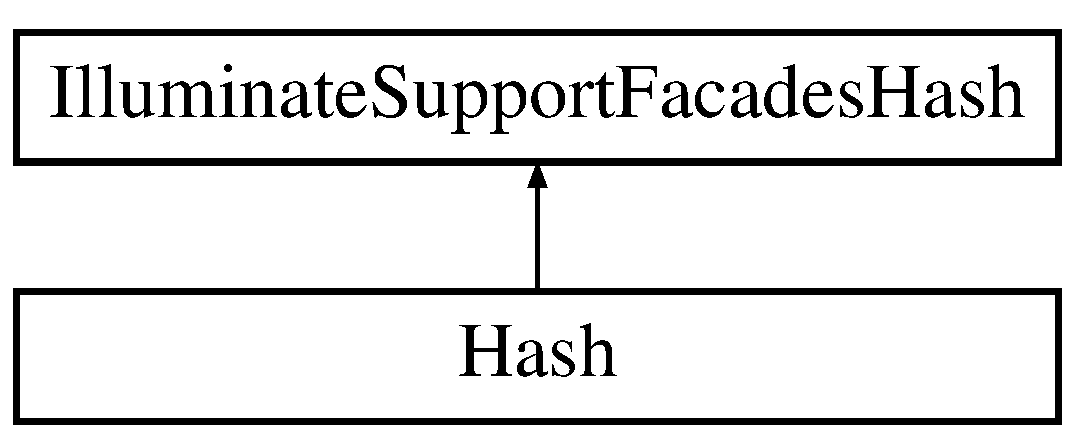
\includegraphics[height=2.000000cm]{class_hash}
\end{center}
\end{figure}
\subsection*{Additional Inherited Members}


The documentation for this class was generated from the following file\+:\begin{DoxyCompactItemize}
\item 
\+\_\+ide\+\_\+helper.\+php\end{DoxyCompactItemize}

\hypertarget{class_illuminate_1_1_support_1_1_facades_1_1_hash}{}\section{Illuminate\textbackslash{}Support\textbackslash{}Facades\textbackslash{}Hash Class Reference}
\label{class_illuminate_1_1_support_1_1_facades_1_1_hash}\index{Illuminate\textbackslash{}\+Support\textbackslash{}\+Facades\textbackslash{}\+Hash@{Illuminate\textbackslash{}\+Support\textbackslash{}\+Facades\textbackslash{}\+Hash}}
Inheritance diagram for Illuminate\textbackslash{}Support\textbackslash{}Facades\textbackslash{}Hash\+:\begin{figure}[H]
\begin{center}
\leavevmode
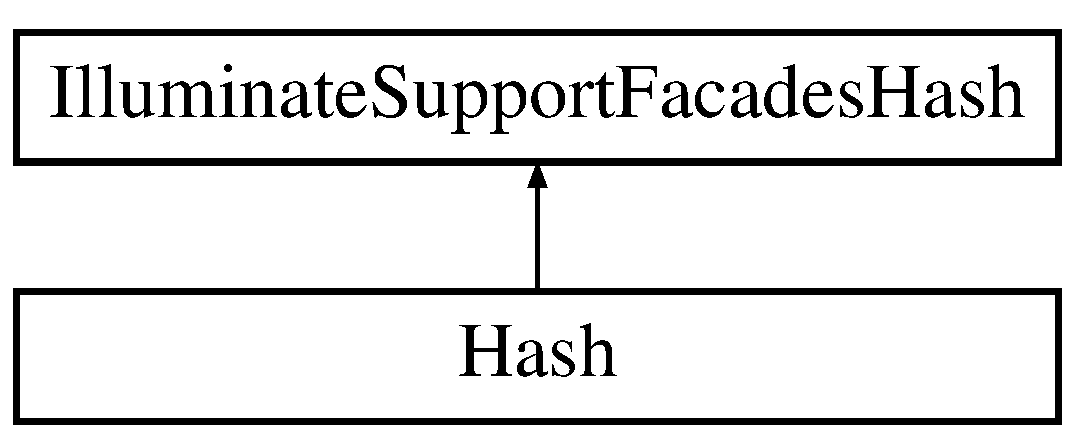
\includegraphics[height=2.000000cm]{class_illuminate_1_1_support_1_1_facades_1_1_hash}
\end{center}
\end{figure}
\subsection*{Static Public Member Functions}
\begin{DoxyCompactItemize}
\item 
static \mbox{\hyperlink{class_illuminate_1_1_support_1_1_facades_1_1_hash_a2a88de88b45fd70857e473c60f0fde51}{make}} (\$value, \$options=array())
\item 
static \mbox{\hyperlink{class_illuminate_1_1_support_1_1_facades_1_1_hash_a4ba83167d6c76b82e6c94b72f2802954}{check}} (\$value, \$hashed\+Value, \$options=array())
\item 
static \mbox{\hyperlink{class_illuminate_1_1_support_1_1_facades_1_1_hash_ace976714a3948b960436eda1da612e3e}{needs\+Rehash}} (\$hashed\+Value, \$options=array())
\item 
static \mbox{\hyperlink{class_illuminate_1_1_support_1_1_facades_1_1_hash_afef6050dcab61a16445707787228a2de}{set\+Rounds}} (\$rounds)
\end{DoxyCompactItemize}


\subsection{Member Function Documentation}
\mbox{\Hypertarget{class_illuminate_1_1_support_1_1_facades_1_1_hash_a4ba83167d6c76b82e6c94b72f2802954}\label{class_illuminate_1_1_support_1_1_facades_1_1_hash_a4ba83167d6c76b82e6c94b72f2802954}} 
\index{Illuminate\+::\+Support\+::\+Facades\+::\+Hash@{Illuminate\+::\+Support\+::\+Facades\+::\+Hash}!check@{check}}
\index{check@{check}!Illuminate\+::\+Support\+::\+Facades\+::\+Hash@{Illuminate\+::\+Support\+::\+Facades\+::\+Hash}}
\subsubsection{\texorpdfstring{check()}{check()}}
{\footnotesize\ttfamily static Illuminate\textbackslash{}\+Support\textbackslash{}\+Facades\textbackslash{}\+Hash\+::check (\begin{DoxyParamCaption}\item[{}]{\$value,  }\item[{}]{\$hashed\+Value,  }\item[{}]{\$options = {\ttfamily array()} }\end{DoxyParamCaption})\hspace{0.3cm}{\ttfamily [static]}}

Check the given plain value against a hash.


\begin{DoxyParams}[1]{Parameters}
string & {\em \$value} & \\
\hline
string & {\em \$hashed\+Value} & \\
\hline
array & {\em \$options} & \\
\hline
\end{DoxyParams}
\begin{DoxyReturn}{Returns}
bool 
\end{DoxyReturn}
\mbox{\Hypertarget{class_illuminate_1_1_support_1_1_facades_1_1_hash_a2a88de88b45fd70857e473c60f0fde51}\label{class_illuminate_1_1_support_1_1_facades_1_1_hash_a2a88de88b45fd70857e473c60f0fde51}} 
\index{Illuminate\+::\+Support\+::\+Facades\+::\+Hash@{Illuminate\+::\+Support\+::\+Facades\+::\+Hash}!make@{make}}
\index{make@{make}!Illuminate\+::\+Support\+::\+Facades\+::\+Hash@{Illuminate\+::\+Support\+::\+Facades\+::\+Hash}}
\subsubsection{\texorpdfstring{make()}{make()}}
{\footnotesize\ttfamily static Illuminate\textbackslash{}\+Support\textbackslash{}\+Facades\textbackslash{}\+Hash\+::make (\begin{DoxyParamCaption}\item[{}]{\$value,  }\item[{}]{\$options = {\ttfamily array()} }\end{DoxyParamCaption})\hspace{0.3cm}{\ttfamily [static]}}

\mbox{\hyperlink{class_illuminate_1_1_support_1_1_facades_1_1_hash}{Hash}} the given value.


\begin{DoxyParams}[1]{Parameters}
string & {\em \$value} & \\
\hline
array & {\em \$options} & \\
\hline
\end{DoxyParams}
\begin{DoxyReturn}{Returns}
string 
\end{DoxyReturn}

\begin{DoxyExceptions}{Exceptions}
{\em } & \\
\hline
\end{DoxyExceptions}
\mbox{\Hypertarget{class_illuminate_1_1_support_1_1_facades_1_1_hash_ace976714a3948b960436eda1da612e3e}\label{class_illuminate_1_1_support_1_1_facades_1_1_hash_ace976714a3948b960436eda1da612e3e}} 
\index{Illuminate\+::\+Support\+::\+Facades\+::\+Hash@{Illuminate\+::\+Support\+::\+Facades\+::\+Hash}!needs\+Rehash@{needs\+Rehash}}
\index{needs\+Rehash@{needs\+Rehash}!Illuminate\+::\+Support\+::\+Facades\+::\+Hash@{Illuminate\+::\+Support\+::\+Facades\+::\+Hash}}
\subsubsection{\texorpdfstring{needs\+Rehash()}{needsRehash()}}
{\footnotesize\ttfamily static Illuminate\textbackslash{}\+Support\textbackslash{}\+Facades\textbackslash{}\+Hash\+::needs\+Rehash (\begin{DoxyParamCaption}\item[{}]{\$hashed\+Value,  }\item[{}]{\$options = {\ttfamily array()} }\end{DoxyParamCaption})\hspace{0.3cm}{\ttfamily [static]}}

Check if the given hash has been hashed using the given options.


\begin{DoxyParams}[1]{Parameters}
string & {\em \$hashed\+Value} & \\
\hline
array & {\em \$options} & \\
\hline
\end{DoxyParams}
\begin{DoxyReturn}{Returns}
bool 
\end{DoxyReturn}
\mbox{\Hypertarget{class_illuminate_1_1_support_1_1_facades_1_1_hash_afef6050dcab61a16445707787228a2de}\label{class_illuminate_1_1_support_1_1_facades_1_1_hash_afef6050dcab61a16445707787228a2de}} 
\index{Illuminate\+::\+Support\+::\+Facades\+::\+Hash@{Illuminate\+::\+Support\+::\+Facades\+::\+Hash}!set\+Rounds@{set\+Rounds}}
\index{set\+Rounds@{set\+Rounds}!Illuminate\+::\+Support\+::\+Facades\+::\+Hash@{Illuminate\+::\+Support\+::\+Facades\+::\+Hash}}
\subsubsection{\texorpdfstring{set\+Rounds()}{setRounds()}}
{\footnotesize\ttfamily static Illuminate\textbackslash{}\+Support\textbackslash{}\+Facades\textbackslash{}\+Hash\+::set\+Rounds (\begin{DoxyParamCaption}\item[{}]{\$rounds }\end{DoxyParamCaption})\hspace{0.3cm}{\ttfamily [static]}}

Set the default password work factor.


\begin{DoxyParams}[1]{Parameters}
int & {\em \$rounds} & \\
\hline
\end{DoxyParams}
\begin{DoxyReturn}{Returns}
\$this 
\end{DoxyReturn}


The documentation for this class was generated from the following file\+:\begin{DoxyCompactItemize}
\item 
\+\_\+ide\+\_\+helper.\+php\end{DoxyCompactItemize}

\hypertarget{class_illuminate_1_1_support_1_1_facades_1_1_lang}{}\section{Illuminate\textbackslash{}Support\textbackslash{}Facades\textbackslash{}Lang Class Reference}
\label{class_illuminate_1_1_support_1_1_facades_1_1_lang}\index{Illuminate\textbackslash{}\+Support\textbackslash{}\+Facades\textbackslash{}\+Lang@{Illuminate\textbackslash{}\+Support\textbackslash{}\+Facades\textbackslash{}\+Lang}}
Inheritance diagram for Illuminate\textbackslash{}Support\textbackslash{}Facades\textbackslash{}Lang\+:\begin{figure}[H]
\begin{center}
\leavevmode
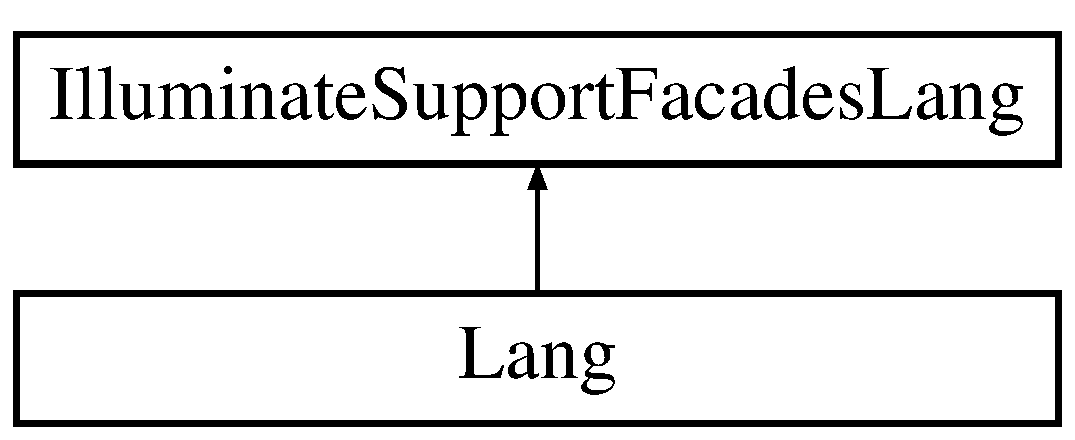
\includegraphics[height=2.000000cm]{class_illuminate_1_1_support_1_1_facades_1_1_lang}
\end{center}
\end{figure}
\subsection*{Static Public Member Functions}
\begin{DoxyCompactItemize}
\item 
static \mbox{\hyperlink{class_illuminate_1_1_support_1_1_facades_1_1_lang_a364ccc2115dc5888b6ed4dd1820f36df}{has\+For\+Locale}} (\$key, \$\mbox{\hyperlink{class_illuminate_1_1_support_1_1_facades_1_1_lang_adf0e7cd50f3430d5e3d7cb161bdfb73c}{locale}}=null)
\item 
static \mbox{\hyperlink{class_illuminate_1_1_support_1_1_facades_1_1_lang_a48506627d20c39b08f17d8dc83ac4be4}{has}} (\$key, \$\mbox{\hyperlink{class_illuminate_1_1_support_1_1_facades_1_1_lang_adf0e7cd50f3430d5e3d7cb161bdfb73c}{locale}}=null, \$fallback=true)
\item 
static \mbox{\hyperlink{class_illuminate_1_1_support_1_1_facades_1_1_lang_a4a3c8c7fd62dea4438d7771b17cb54ac}{trans}} (\$key, \$replace=array(), \$\mbox{\hyperlink{class_illuminate_1_1_support_1_1_facades_1_1_lang_adf0e7cd50f3430d5e3d7cb161bdfb73c}{locale}}=null)
\item 
static \mbox{\hyperlink{class_illuminate_1_1_support_1_1_facades_1_1_lang_af707bce83f27a25456bcfb084c0244dc}{get}} (\$key, \$replace=array(), \$\mbox{\hyperlink{class_illuminate_1_1_support_1_1_facades_1_1_lang_adf0e7cd50f3430d5e3d7cb161bdfb73c}{locale}}=null, \$fallback=true)
\item 
static \mbox{\hyperlink{class_illuminate_1_1_support_1_1_facades_1_1_lang_aa93883fd367d20be584bbabb383d7fb3}{get\+From\+Json}} (\$key, \$replace=array(), \$\mbox{\hyperlink{class_illuminate_1_1_support_1_1_facades_1_1_lang_adf0e7cd50f3430d5e3d7cb161bdfb73c}{locale}}=null)
\item 
static \mbox{\hyperlink{class_illuminate_1_1_support_1_1_facades_1_1_lang_aa37c675b9e5dc2a74f4237873ddaad71}{trans\+Choice}} (\$key, \$number, \$replace=array(), \$\mbox{\hyperlink{class_illuminate_1_1_support_1_1_facades_1_1_lang_adf0e7cd50f3430d5e3d7cb161bdfb73c}{locale}}=null)
\item 
static \mbox{\hyperlink{class_illuminate_1_1_support_1_1_facades_1_1_lang_a6bba86653ed5618ecafd2381900e69f2}{choice}} (\$key, \$number, \$replace=array(), \$\mbox{\hyperlink{class_illuminate_1_1_support_1_1_facades_1_1_lang_adf0e7cd50f3430d5e3d7cb161bdfb73c}{locale}}=null)
\item 
static \mbox{\hyperlink{class_illuminate_1_1_support_1_1_facades_1_1_lang_ae87d32a21d89d3955844b7fc06cc24cb}{add\+Lines}} (\$lines, \$\mbox{\hyperlink{class_illuminate_1_1_support_1_1_facades_1_1_lang_adf0e7cd50f3430d5e3d7cb161bdfb73c}{locale}}, \$namespace=\textquotesingle{} $\ast$\textquotesingle{})
\item 
static \mbox{\hyperlink{class_illuminate_1_1_support_1_1_facades_1_1_lang_afb16817981fd372ac47c226b11acba78}{load}} (\$namespace, \$group, \$\mbox{\hyperlink{class_illuminate_1_1_support_1_1_facades_1_1_lang_adf0e7cd50f3430d5e3d7cb161bdfb73c}{locale}})
\item 
static \mbox{\hyperlink{class_illuminate_1_1_support_1_1_facades_1_1_lang_a4fd7b406202d15b9d5e7091a272561f4}{add\+Namespace}} (\$namespace, \$hint)
\item 
static \mbox{\hyperlink{class_illuminate_1_1_support_1_1_facades_1_1_lang_afdbb701cfcbae342151a3feb292a3a47}{add\+Json\+Path}} (\$path)
\item 
static \mbox{\hyperlink{class_illuminate_1_1_support_1_1_facades_1_1_lang_aac2a9b78d2633d1ded279422f448576d}{parse\+Key}} (\$key)
\item 
static \mbox{\hyperlink{class_illuminate_1_1_support_1_1_facades_1_1_lang_a783b77c9beca28357274d4abb92f65ad}{get\+Selector}} ()
\item 
static \mbox{\hyperlink{class_illuminate_1_1_support_1_1_facades_1_1_lang_a99b0d2353fea13c5c8d750daba6c1c10}{set\+Selector}} (\$selector)
\item 
static \mbox{\hyperlink{class_illuminate_1_1_support_1_1_facades_1_1_lang_a681996518ed5da981ade1a58c4c70b25}{get\+Loader}} ()
\item 
static \mbox{\hyperlink{class_illuminate_1_1_support_1_1_facades_1_1_lang_adf0e7cd50f3430d5e3d7cb161bdfb73c}{locale}} ()
\item 
static \mbox{\hyperlink{class_illuminate_1_1_support_1_1_facades_1_1_lang_a86a2fd3dd1b3a5973a5abb1aa7314357}{get\+Locale}} ()
\item 
static \mbox{\hyperlink{class_illuminate_1_1_support_1_1_facades_1_1_lang_aee5fdf1c926d12ee4c071974ad8303e4}{set\+Locale}} (\$\mbox{\hyperlink{class_illuminate_1_1_support_1_1_facades_1_1_lang_adf0e7cd50f3430d5e3d7cb161bdfb73c}{locale}})
\item 
static \mbox{\hyperlink{class_illuminate_1_1_support_1_1_facades_1_1_lang_ab0db39913768af6f4421548ae334ba30}{get\+Fallback}} ()
\item 
static \mbox{\hyperlink{class_illuminate_1_1_support_1_1_facades_1_1_lang_a36c9cbddc88f2629de99fd88097d911b}{set\+Fallback}} (\$fallback)
\item 
static \mbox{\hyperlink{class_illuminate_1_1_support_1_1_facades_1_1_lang_a604716b0f8afe89d3597a81029037fcd}{set\+Parsed\+Key}} (\$key, \$parsed)
\item 
static \mbox{\hyperlink{class_illuminate_1_1_support_1_1_facades_1_1_lang_a0df95ccd871c7765ec279319e3d75556}{macro}} (\$name, \$macro)
\item 
static \mbox{\hyperlink{class_illuminate_1_1_support_1_1_facades_1_1_lang_a683a95badc6642bc4f01b18e07cf4640}{mixin}} (\$mixin)
\item 
static \mbox{\hyperlink{class_illuminate_1_1_support_1_1_facades_1_1_lang_a38c28fa8a1fcb752424e16b536341ce5}{has\+Macro}} (\$name)
\end{DoxyCompactItemize}


\subsection{Member Function Documentation}
\mbox{\Hypertarget{class_illuminate_1_1_support_1_1_facades_1_1_lang_afdbb701cfcbae342151a3feb292a3a47}\label{class_illuminate_1_1_support_1_1_facades_1_1_lang_afdbb701cfcbae342151a3feb292a3a47}} 
\index{Illuminate\+::\+Support\+::\+Facades\+::\+Lang@{Illuminate\+::\+Support\+::\+Facades\+::\+Lang}!add\+Json\+Path@{add\+Json\+Path}}
\index{add\+Json\+Path@{add\+Json\+Path}!Illuminate\+::\+Support\+::\+Facades\+::\+Lang@{Illuminate\+::\+Support\+::\+Facades\+::\+Lang}}
\subsubsection{\texorpdfstring{add\+Json\+Path()}{addJsonPath()}}
{\footnotesize\ttfamily static Illuminate\textbackslash{}\+Support\textbackslash{}\+Facades\textbackslash{}\+Lang\+::add\+Json\+Path (\begin{DoxyParamCaption}\item[{}]{\$path }\end{DoxyParamCaption})\hspace{0.3cm}{\ttfamily [static]}}

Add a new J\+S\+ON path to the loader.


\begin{DoxyParams}[1]{Parameters}
string & {\em \$path} & \\
\hline
\end{DoxyParams}
\begin{DoxyReturn}{Returns}
void 
\end{DoxyReturn}
\mbox{\Hypertarget{class_illuminate_1_1_support_1_1_facades_1_1_lang_ae87d32a21d89d3955844b7fc06cc24cb}\label{class_illuminate_1_1_support_1_1_facades_1_1_lang_ae87d32a21d89d3955844b7fc06cc24cb}} 
\index{Illuminate\+::\+Support\+::\+Facades\+::\+Lang@{Illuminate\+::\+Support\+::\+Facades\+::\+Lang}!add\+Lines@{add\+Lines}}
\index{add\+Lines@{add\+Lines}!Illuminate\+::\+Support\+::\+Facades\+::\+Lang@{Illuminate\+::\+Support\+::\+Facades\+::\+Lang}}
\subsubsection{\texorpdfstring{add\+Lines()}{addLines()}}
{\footnotesize\ttfamily static Illuminate\textbackslash{}\+Support\textbackslash{}\+Facades\textbackslash{}\+Lang\+::add\+Lines (\begin{DoxyParamCaption}\item[{}]{\$lines,  }\item[{}]{\$locale,  }\item[{}]{\$namespace = {\ttfamily \textquotesingle{}$\ast$\textquotesingle{}} }\end{DoxyParamCaption})\hspace{0.3cm}{\ttfamily [static]}}

Add translation lines to the given locale.


\begin{DoxyParams}[1]{Parameters}
array & {\em \$lines} & \\
\hline
string & {\em \$locale} & \\
\hline
string & {\em \$namespace} & \\
\hline
\end{DoxyParams}
\begin{DoxyReturn}{Returns}
void 
\end{DoxyReturn}
\mbox{\Hypertarget{class_illuminate_1_1_support_1_1_facades_1_1_lang_a4fd7b406202d15b9d5e7091a272561f4}\label{class_illuminate_1_1_support_1_1_facades_1_1_lang_a4fd7b406202d15b9d5e7091a272561f4}} 
\index{Illuminate\+::\+Support\+::\+Facades\+::\+Lang@{Illuminate\+::\+Support\+::\+Facades\+::\+Lang}!add\+Namespace@{add\+Namespace}}
\index{add\+Namespace@{add\+Namespace}!Illuminate\+::\+Support\+::\+Facades\+::\+Lang@{Illuminate\+::\+Support\+::\+Facades\+::\+Lang}}
\subsubsection{\texorpdfstring{add\+Namespace()}{addNamespace()}}
{\footnotesize\ttfamily static Illuminate\textbackslash{}\+Support\textbackslash{}\+Facades\textbackslash{}\+Lang\+::add\+Namespace (\begin{DoxyParamCaption}\item[{}]{\$namespace,  }\item[{}]{\$hint }\end{DoxyParamCaption})\hspace{0.3cm}{\ttfamily [static]}}

Add a new namespace to the loader.


\begin{DoxyParams}[1]{Parameters}
string & {\em \$namespace} & \\
\hline
string & {\em \$hint} & \\
\hline
\end{DoxyParams}
\begin{DoxyReturn}{Returns}
void 
\end{DoxyReturn}
\mbox{\Hypertarget{class_illuminate_1_1_support_1_1_facades_1_1_lang_a6bba86653ed5618ecafd2381900e69f2}\label{class_illuminate_1_1_support_1_1_facades_1_1_lang_a6bba86653ed5618ecafd2381900e69f2}} 
\index{Illuminate\+::\+Support\+::\+Facades\+::\+Lang@{Illuminate\+::\+Support\+::\+Facades\+::\+Lang}!choice@{choice}}
\index{choice@{choice}!Illuminate\+::\+Support\+::\+Facades\+::\+Lang@{Illuminate\+::\+Support\+::\+Facades\+::\+Lang}}
\subsubsection{\texorpdfstring{choice()}{choice()}}
{\footnotesize\ttfamily static Illuminate\textbackslash{}\+Support\textbackslash{}\+Facades\textbackslash{}\+Lang\+::choice (\begin{DoxyParamCaption}\item[{}]{\$key,  }\item[{}]{\$number,  }\item[{}]{\$replace = {\ttfamily array()},  }\item[{}]{\$locale = {\ttfamily null} }\end{DoxyParamCaption})\hspace{0.3cm}{\ttfamily [static]}}

Get a translation according to an integer value.


\begin{DoxyParams}[1]{Parameters}
string & {\em \$key} & \\
\hline
int | array | \textbackslash{}\+Countable & {\em \$number} & \\
\hline
array & {\em \$replace} & \\
\hline
string & {\em \$locale} & \\
\hline
\end{DoxyParams}
\begin{DoxyReturn}{Returns}
string 
\end{DoxyReturn}
\mbox{\Hypertarget{class_illuminate_1_1_support_1_1_facades_1_1_lang_af707bce83f27a25456bcfb084c0244dc}\label{class_illuminate_1_1_support_1_1_facades_1_1_lang_af707bce83f27a25456bcfb084c0244dc}} 
\index{Illuminate\+::\+Support\+::\+Facades\+::\+Lang@{Illuminate\+::\+Support\+::\+Facades\+::\+Lang}!get@{get}}
\index{get@{get}!Illuminate\+::\+Support\+::\+Facades\+::\+Lang@{Illuminate\+::\+Support\+::\+Facades\+::\+Lang}}
\subsubsection{\texorpdfstring{get()}{get()}}
{\footnotesize\ttfamily static Illuminate\textbackslash{}\+Support\textbackslash{}\+Facades\textbackslash{}\+Lang\+::get (\begin{DoxyParamCaption}\item[{}]{\$key,  }\item[{}]{\$replace = {\ttfamily array()},  }\item[{}]{\$locale = {\ttfamily null},  }\item[{}]{\$fallback = {\ttfamily true} }\end{DoxyParamCaption})\hspace{0.3cm}{\ttfamily [static]}}

Get the translation for the given key.


\begin{DoxyParams}[1]{Parameters}
string & {\em \$key} & \\
\hline
array & {\em \$replace} & \\
\hline
string | null & {\em \$locale} & \\
\hline
bool & {\em \$fallback} & \\
\hline
\end{DoxyParams}
\begin{DoxyReturn}{Returns}
string$\vert$array$\vert$null 
\end{DoxyReturn}
\mbox{\Hypertarget{class_illuminate_1_1_support_1_1_facades_1_1_lang_ab0db39913768af6f4421548ae334ba30}\label{class_illuminate_1_1_support_1_1_facades_1_1_lang_ab0db39913768af6f4421548ae334ba30}} 
\index{Illuminate\+::\+Support\+::\+Facades\+::\+Lang@{Illuminate\+::\+Support\+::\+Facades\+::\+Lang}!get\+Fallback@{get\+Fallback}}
\index{get\+Fallback@{get\+Fallback}!Illuminate\+::\+Support\+::\+Facades\+::\+Lang@{Illuminate\+::\+Support\+::\+Facades\+::\+Lang}}
\subsubsection{\texorpdfstring{get\+Fallback()}{getFallback()}}
{\footnotesize\ttfamily static Illuminate\textbackslash{}\+Support\textbackslash{}\+Facades\textbackslash{}\+Lang\+::get\+Fallback (\begin{DoxyParamCaption}{ }\end{DoxyParamCaption})\hspace{0.3cm}{\ttfamily [static]}}

Get the fallback locale being used.

\begin{DoxyReturn}{Returns}
string 
\end{DoxyReturn}
\mbox{\Hypertarget{class_illuminate_1_1_support_1_1_facades_1_1_lang_aa93883fd367d20be584bbabb383d7fb3}\label{class_illuminate_1_1_support_1_1_facades_1_1_lang_aa93883fd367d20be584bbabb383d7fb3}} 
\index{Illuminate\+::\+Support\+::\+Facades\+::\+Lang@{Illuminate\+::\+Support\+::\+Facades\+::\+Lang}!get\+From\+Json@{get\+From\+Json}}
\index{get\+From\+Json@{get\+From\+Json}!Illuminate\+::\+Support\+::\+Facades\+::\+Lang@{Illuminate\+::\+Support\+::\+Facades\+::\+Lang}}
\subsubsection{\texorpdfstring{get\+From\+Json()}{getFromJson()}}
{\footnotesize\ttfamily static Illuminate\textbackslash{}\+Support\textbackslash{}\+Facades\textbackslash{}\+Lang\+::get\+From\+Json (\begin{DoxyParamCaption}\item[{}]{\$key,  }\item[{}]{\$replace = {\ttfamily array()},  }\item[{}]{\$locale = {\ttfamily null} }\end{DoxyParamCaption})\hspace{0.3cm}{\ttfamily [static]}}

Get the translation for a given key from the J\+S\+ON translation files.


\begin{DoxyParams}[1]{Parameters}
string & {\em \$key} & \\
\hline
array & {\em \$replace} & \\
\hline
string & {\em \$locale} & \\
\hline
\end{DoxyParams}
\begin{DoxyReturn}{Returns}
string 
\end{DoxyReturn}
\mbox{\Hypertarget{class_illuminate_1_1_support_1_1_facades_1_1_lang_a681996518ed5da981ade1a58c4c70b25}\label{class_illuminate_1_1_support_1_1_facades_1_1_lang_a681996518ed5da981ade1a58c4c70b25}} 
\index{Illuminate\+::\+Support\+::\+Facades\+::\+Lang@{Illuminate\+::\+Support\+::\+Facades\+::\+Lang}!get\+Loader@{get\+Loader}}
\index{get\+Loader@{get\+Loader}!Illuminate\+::\+Support\+::\+Facades\+::\+Lang@{Illuminate\+::\+Support\+::\+Facades\+::\+Lang}}
\subsubsection{\texorpdfstring{get\+Loader()}{getLoader()}}
{\footnotesize\ttfamily static Illuminate\textbackslash{}\+Support\textbackslash{}\+Facades\textbackslash{}\+Lang\+::get\+Loader (\begin{DoxyParamCaption}{ }\end{DoxyParamCaption})\hspace{0.3cm}{\ttfamily [static]}}

Get the language line loader implementation.

\begin{DoxyReturn}{Returns}

\end{DoxyReturn}
\mbox{\Hypertarget{class_illuminate_1_1_support_1_1_facades_1_1_lang_a86a2fd3dd1b3a5973a5abb1aa7314357}\label{class_illuminate_1_1_support_1_1_facades_1_1_lang_a86a2fd3dd1b3a5973a5abb1aa7314357}} 
\index{Illuminate\+::\+Support\+::\+Facades\+::\+Lang@{Illuminate\+::\+Support\+::\+Facades\+::\+Lang}!get\+Locale@{get\+Locale}}
\index{get\+Locale@{get\+Locale}!Illuminate\+::\+Support\+::\+Facades\+::\+Lang@{Illuminate\+::\+Support\+::\+Facades\+::\+Lang}}
\subsubsection{\texorpdfstring{get\+Locale()}{getLocale()}}
{\footnotesize\ttfamily static Illuminate\textbackslash{}\+Support\textbackslash{}\+Facades\textbackslash{}\+Lang\+::get\+Locale (\begin{DoxyParamCaption}{ }\end{DoxyParamCaption})\hspace{0.3cm}{\ttfamily [static]}}

Get the default locale being used.

\begin{DoxyReturn}{Returns}
string 
\end{DoxyReturn}
\mbox{\Hypertarget{class_illuminate_1_1_support_1_1_facades_1_1_lang_a783b77c9beca28357274d4abb92f65ad}\label{class_illuminate_1_1_support_1_1_facades_1_1_lang_a783b77c9beca28357274d4abb92f65ad}} 
\index{Illuminate\+::\+Support\+::\+Facades\+::\+Lang@{Illuminate\+::\+Support\+::\+Facades\+::\+Lang}!get\+Selector@{get\+Selector}}
\index{get\+Selector@{get\+Selector}!Illuminate\+::\+Support\+::\+Facades\+::\+Lang@{Illuminate\+::\+Support\+::\+Facades\+::\+Lang}}
\subsubsection{\texorpdfstring{get\+Selector()}{getSelector()}}
{\footnotesize\ttfamily static Illuminate\textbackslash{}\+Support\textbackslash{}\+Facades\textbackslash{}\+Lang\+::get\+Selector (\begin{DoxyParamCaption}{ }\end{DoxyParamCaption})\hspace{0.3cm}{\ttfamily [static]}}

Get the message selector instance.

\begin{DoxyReturn}{Returns}

\end{DoxyReturn}
\mbox{\Hypertarget{class_illuminate_1_1_support_1_1_facades_1_1_lang_a48506627d20c39b08f17d8dc83ac4be4}\label{class_illuminate_1_1_support_1_1_facades_1_1_lang_a48506627d20c39b08f17d8dc83ac4be4}} 
\index{Illuminate\+::\+Support\+::\+Facades\+::\+Lang@{Illuminate\+::\+Support\+::\+Facades\+::\+Lang}!has@{has}}
\index{has@{has}!Illuminate\+::\+Support\+::\+Facades\+::\+Lang@{Illuminate\+::\+Support\+::\+Facades\+::\+Lang}}
\subsubsection{\texorpdfstring{has()}{has()}}
{\footnotesize\ttfamily static Illuminate\textbackslash{}\+Support\textbackslash{}\+Facades\textbackslash{}\+Lang\+::has (\begin{DoxyParamCaption}\item[{}]{\$key,  }\item[{}]{\$locale = {\ttfamily null},  }\item[{}]{\$fallback = {\ttfamily true} }\end{DoxyParamCaption})\hspace{0.3cm}{\ttfamily [static]}}

Determine if a translation exists.


\begin{DoxyParams}[1]{Parameters}
string & {\em \$key} & \\
\hline
string | null & {\em \$locale} & \\
\hline
bool & {\em \$fallback} & \\
\hline
\end{DoxyParams}
\begin{DoxyReturn}{Returns}
bool 
\end{DoxyReturn}
\mbox{\Hypertarget{class_illuminate_1_1_support_1_1_facades_1_1_lang_a364ccc2115dc5888b6ed4dd1820f36df}\label{class_illuminate_1_1_support_1_1_facades_1_1_lang_a364ccc2115dc5888b6ed4dd1820f36df}} 
\index{Illuminate\+::\+Support\+::\+Facades\+::\+Lang@{Illuminate\+::\+Support\+::\+Facades\+::\+Lang}!has\+For\+Locale@{has\+For\+Locale}}
\index{has\+For\+Locale@{has\+For\+Locale}!Illuminate\+::\+Support\+::\+Facades\+::\+Lang@{Illuminate\+::\+Support\+::\+Facades\+::\+Lang}}
\subsubsection{\texorpdfstring{has\+For\+Locale()}{hasForLocale()}}
{\footnotesize\ttfamily static Illuminate\textbackslash{}\+Support\textbackslash{}\+Facades\textbackslash{}\+Lang\+::has\+For\+Locale (\begin{DoxyParamCaption}\item[{}]{\$key,  }\item[{}]{\$locale = {\ttfamily null} }\end{DoxyParamCaption})\hspace{0.3cm}{\ttfamily [static]}}

Determine if a translation exists for a given locale.


\begin{DoxyParams}[1]{Parameters}
string & {\em \$key} & \\
\hline
string | null & {\em \$locale} & \\
\hline
\end{DoxyParams}
\begin{DoxyReturn}{Returns}
bool 
\end{DoxyReturn}
\mbox{\Hypertarget{class_illuminate_1_1_support_1_1_facades_1_1_lang_a38c28fa8a1fcb752424e16b536341ce5}\label{class_illuminate_1_1_support_1_1_facades_1_1_lang_a38c28fa8a1fcb752424e16b536341ce5}} 
\index{Illuminate\+::\+Support\+::\+Facades\+::\+Lang@{Illuminate\+::\+Support\+::\+Facades\+::\+Lang}!has\+Macro@{has\+Macro}}
\index{has\+Macro@{has\+Macro}!Illuminate\+::\+Support\+::\+Facades\+::\+Lang@{Illuminate\+::\+Support\+::\+Facades\+::\+Lang}}
\subsubsection{\texorpdfstring{has\+Macro()}{hasMacro()}}
{\footnotesize\ttfamily static Illuminate\textbackslash{}\+Support\textbackslash{}\+Facades\textbackslash{}\+Lang\+::has\+Macro (\begin{DoxyParamCaption}\item[{}]{\$name }\end{DoxyParamCaption})\hspace{0.3cm}{\ttfamily [static]}}

Checks if macro is registered.


\begin{DoxyParams}[1]{Parameters}
string & {\em \$name} & \\
\hline
\end{DoxyParams}
\begin{DoxyReturn}{Returns}
bool 
\end{DoxyReturn}
\mbox{\Hypertarget{class_illuminate_1_1_support_1_1_facades_1_1_lang_afb16817981fd372ac47c226b11acba78}\label{class_illuminate_1_1_support_1_1_facades_1_1_lang_afb16817981fd372ac47c226b11acba78}} 
\index{Illuminate\+::\+Support\+::\+Facades\+::\+Lang@{Illuminate\+::\+Support\+::\+Facades\+::\+Lang}!load@{load}}
\index{load@{load}!Illuminate\+::\+Support\+::\+Facades\+::\+Lang@{Illuminate\+::\+Support\+::\+Facades\+::\+Lang}}
\subsubsection{\texorpdfstring{load()}{load()}}
{\footnotesize\ttfamily static Illuminate\textbackslash{}\+Support\textbackslash{}\+Facades\textbackslash{}\+Lang\+::load (\begin{DoxyParamCaption}\item[{}]{\$namespace,  }\item[{}]{\$group,  }\item[{}]{\$locale }\end{DoxyParamCaption})\hspace{0.3cm}{\ttfamily [static]}}

Load the specified language group.


\begin{DoxyParams}[1]{Parameters}
string & {\em \$namespace} & \\
\hline
string & {\em \$group} & \\
\hline
string & {\em \$locale} & \\
\hline
\end{DoxyParams}
\begin{DoxyReturn}{Returns}
void 
\end{DoxyReturn}
\mbox{\Hypertarget{class_illuminate_1_1_support_1_1_facades_1_1_lang_adf0e7cd50f3430d5e3d7cb161bdfb73c}\label{class_illuminate_1_1_support_1_1_facades_1_1_lang_adf0e7cd50f3430d5e3d7cb161bdfb73c}} 
\index{Illuminate\+::\+Support\+::\+Facades\+::\+Lang@{Illuminate\+::\+Support\+::\+Facades\+::\+Lang}!locale@{locale}}
\index{locale@{locale}!Illuminate\+::\+Support\+::\+Facades\+::\+Lang@{Illuminate\+::\+Support\+::\+Facades\+::\+Lang}}
\subsubsection{\texorpdfstring{locale()}{locale()}}
{\footnotesize\ttfamily static Illuminate\textbackslash{}\+Support\textbackslash{}\+Facades\textbackslash{}\+Lang\+::locale (\begin{DoxyParamCaption}{ }\end{DoxyParamCaption})\hspace{0.3cm}{\ttfamily [static]}}

Get the default locale being used.

\begin{DoxyReturn}{Returns}
string 
\end{DoxyReturn}
\mbox{\Hypertarget{class_illuminate_1_1_support_1_1_facades_1_1_lang_a0df95ccd871c7765ec279319e3d75556}\label{class_illuminate_1_1_support_1_1_facades_1_1_lang_a0df95ccd871c7765ec279319e3d75556}} 
\index{Illuminate\+::\+Support\+::\+Facades\+::\+Lang@{Illuminate\+::\+Support\+::\+Facades\+::\+Lang}!macro@{macro}}
\index{macro@{macro}!Illuminate\+::\+Support\+::\+Facades\+::\+Lang@{Illuminate\+::\+Support\+::\+Facades\+::\+Lang}}
\subsubsection{\texorpdfstring{macro()}{macro()}}
{\footnotesize\ttfamily static Illuminate\textbackslash{}\+Support\textbackslash{}\+Facades\textbackslash{}\+Lang\+::macro (\begin{DoxyParamCaption}\item[{}]{\$name,  }\item[{}]{\$macro }\end{DoxyParamCaption})\hspace{0.3cm}{\ttfamily [static]}}

Register a custom macro.


\begin{DoxyParams}[1]{Parameters}
string & {\em \$name} & \\
\hline
object | callable & {\em \$macro} & \\
\hline
\end{DoxyParams}
\begin{DoxyReturn}{Returns}
void 
\end{DoxyReturn}
\mbox{\Hypertarget{class_illuminate_1_1_support_1_1_facades_1_1_lang_a683a95badc6642bc4f01b18e07cf4640}\label{class_illuminate_1_1_support_1_1_facades_1_1_lang_a683a95badc6642bc4f01b18e07cf4640}} 
\index{Illuminate\+::\+Support\+::\+Facades\+::\+Lang@{Illuminate\+::\+Support\+::\+Facades\+::\+Lang}!mixin@{mixin}}
\index{mixin@{mixin}!Illuminate\+::\+Support\+::\+Facades\+::\+Lang@{Illuminate\+::\+Support\+::\+Facades\+::\+Lang}}
\subsubsection{\texorpdfstring{mixin()}{mixin()}}
{\footnotesize\ttfamily static Illuminate\textbackslash{}\+Support\textbackslash{}\+Facades\textbackslash{}\+Lang\+::mixin (\begin{DoxyParamCaption}\item[{}]{\$mixin }\end{DoxyParamCaption})\hspace{0.3cm}{\ttfamily [static]}}

Mix another object into the class.


\begin{DoxyParams}[1]{Parameters}
object & {\em \$mixin} & \\
\hline
\end{DoxyParams}
\begin{DoxyReturn}{Returns}
void 
\end{DoxyReturn}
\mbox{\Hypertarget{class_illuminate_1_1_support_1_1_facades_1_1_lang_aac2a9b78d2633d1ded279422f448576d}\label{class_illuminate_1_1_support_1_1_facades_1_1_lang_aac2a9b78d2633d1ded279422f448576d}} 
\index{Illuminate\+::\+Support\+::\+Facades\+::\+Lang@{Illuminate\+::\+Support\+::\+Facades\+::\+Lang}!parse\+Key@{parse\+Key}}
\index{parse\+Key@{parse\+Key}!Illuminate\+::\+Support\+::\+Facades\+::\+Lang@{Illuminate\+::\+Support\+::\+Facades\+::\+Lang}}
\subsubsection{\texorpdfstring{parse\+Key()}{parseKey()}}
{\footnotesize\ttfamily static Illuminate\textbackslash{}\+Support\textbackslash{}\+Facades\textbackslash{}\+Lang\+::parse\+Key (\begin{DoxyParamCaption}\item[{}]{\$key }\end{DoxyParamCaption})\hspace{0.3cm}{\ttfamily [static]}}

Parse a key into namespace, group, and item.


\begin{DoxyParams}[1]{Parameters}
string & {\em \$key} & \\
\hline
\end{DoxyParams}
\begin{DoxyReturn}{Returns}
array 
\end{DoxyReturn}
\mbox{\Hypertarget{class_illuminate_1_1_support_1_1_facades_1_1_lang_a36c9cbddc88f2629de99fd88097d911b}\label{class_illuminate_1_1_support_1_1_facades_1_1_lang_a36c9cbddc88f2629de99fd88097d911b}} 
\index{Illuminate\+::\+Support\+::\+Facades\+::\+Lang@{Illuminate\+::\+Support\+::\+Facades\+::\+Lang}!set\+Fallback@{set\+Fallback}}
\index{set\+Fallback@{set\+Fallback}!Illuminate\+::\+Support\+::\+Facades\+::\+Lang@{Illuminate\+::\+Support\+::\+Facades\+::\+Lang}}
\subsubsection{\texorpdfstring{set\+Fallback()}{setFallback()}}
{\footnotesize\ttfamily static Illuminate\textbackslash{}\+Support\textbackslash{}\+Facades\textbackslash{}\+Lang\+::set\+Fallback (\begin{DoxyParamCaption}\item[{}]{\$fallback }\end{DoxyParamCaption})\hspace{0.3cm}{\ttfamily [static]}}

Set the fallback locale being used.


\begin{DoxyParams}[1]{Parameters}
string & {\em \$fallback} & \\
\hline
\end{DoxyParams}
\begin{DoxyReturn}{Returns}
void 
\end{DoxyReturn}
\mbox{\Hypertarget{class_illuminate_1_1_support_1_1_facades_1_1_lang_aee5fdf1c926d12ee4c071974ad8303e4}\label{class_illuminate_1_1_support_1_1_facades_1_1_lang_aee5fdf1c926d12ee4c071974ad8303e4}} 
\index{Illuminate\+::\+Support\+::\+Facades\+::\+Lang@{Illuminate\+::\+Support\+::\+Facades\+::\+Lang}!set\+Locale@{set\+Locale}}
\index{set\+Locale@{set\+Locale}!Illuminate\+::\+Support\+::\+Facades\+::\+Lang@{Illuminate\+::\+Support\+::\+Facades\+::\+Lang}}
\subsubsection{\texorpdfstring{set\+Locale()}{setLocale()}}
{\footnotesize\ttfamily static Illuminate\textbackslash{}\+Support\textbackslash{}\+Facades\textbackslash{}\+Lang\+::set\+Locale (\begin{DoxyParamCaption}\item[{}]{\$locale }\end{DoxyParamCaption})\hspace{0.3cm}{\ttfamily [static]}}

Set the default locale.


\begin{DoxyParams}[1]{Parameters}
string & {\em \$locale} & \\
\hline
\end{DoxyParams}
\begin{DoxyReturn}{Returns}
void 
\end{DoxyReturn}
\mbox{\Hypertarget{class_illuminate_1_1_support_1_1_facades_1_1_lang_a604716b0f8afe89d3597a81029037fcd}\label{class_illuminate_1_1_support_1_1_facades_1_1_lang_a604716b0f8afe89d3597a81029037fcd}} 
\index{Illuminate\+::\+Support\+::\+Facades\+::\+Lang@{Illuminate\+::\+Support\+::\+Facades\+::\+Lang}!set\+Parsed\+Key@{set\+Parsed\+Key}}
\index{set\+Parsed\+Key@{set\+Parsed\+Key}!Illuminate\+::\+Support\+::\+Facades\+::\+Lang@{Illuminate\+::\+Support\+::\+Facades\+::\+Lang}}
\subsubsection{\texorpdfstring{set\+Parsed\+Key()}{setParsedKey()}}
{\footnotesize\ttfamily static Illuminate\textbackslash{}\+Support\textbackslash{}\+Facades\textbackslash{}\+Lang\+::set\+Parsed\+Key (\begin{DoxyParamCaption}\item[{}]{\$key,  }\item[{}]{\$parsed }\end{DoxyParamCaption})\hspace{0.3cm}{\ttfamily [static]}}

Set the parsed value of a key.


\begin{DoxyParams}[1]{Parameters}
string & {\em \$key} & \\
\hline
array & {\em \$parsed} & \\
\hline
\end{DoxyParams}
\begin{DoxyReturn}{Returns}
void 
\end{DoxyReturn}
\mbox{\Hypertarget{class_illuminate_1_1_support_1_1_facades_1_1_lang_a99b0d2353fea13c5c8d750daba6c1c10}\label{class_illuminate_1_1_support_1_1_facades_1_1_lang_a99b0d2353fea13c5c8d750daba6c1c10}} 
\index{Illuminate\+::\+Support\+::\+Facades\+::\+Lang@{Illuminate\+::\+Support\+::\+Facades\+::\+Lang}!set\+Selector@{set\+Selector}}
\index{set\+Selector@{set\+Selector}!Illuminate\+::\+Support\+::\+Facades\+::\+Lang@{Illuminate\+::\+Support\+::\+Facades\+::\+Lang}}
\subsubsection{\texorpdfstring{set\+Selector()}{setSelector()}}
{\footnotesize\ttfamily static Illuminate\textbackslash{}\+Support\textbackslash{}\+Facades\textbackslash{}\+Lang\+::set\+Selector (\begin{DoxyParamCaption}\item[{}]{\$selector }\end{DoxyParamCaption})\hspace{0.3cm}{\ttfamily [static]}}

Set the message selector instance.


\begin{DoxyParams}[1]{Parameters}
\textbackslash{}\+Illuminate\textbackslash{}\+Translation\textbackslash{}\+Message\+Selector & {\em \$selector} & \\
\hline
\end{DoxyParams}
\begin{DoxyReturn}{Returns}
void 
\end{DoxyReturn}
\mbox{\Hypertarget{class_illuminate_1_1_support_1_1_facades_1_1_lang_a4a3c8c7fd62dea4438d7771b17cb54ac}\label{class_illuminate_1_1_support_1_1_facades_1_1_lang_a4a3c8c7fd62dea4438d7771b17cb54ac}} 
\index{Illuminate\+::\+Support\+::\+Facades\+::\+Lang@{Illuminate\+::\+Support\+::\+Facades\+::\+Lang}!trans@{trans}}
\index{trans@{trans}!Illuminate\+::\+Support\+::\+Facades\+::\+Lang@{Illuminate\+::\+Support\+::\+Facades\+::\+Lang}}
\subsubsection{\texorpdfstring{trans()}{trans()}}
{\footnotesize\ttfamily static Illuminate\textbackslash{}\+Support\textbackslash{}\+Facades\textbackslash{}\+Lang\+::trans (\begin{DoxyParamCaption}\item[{}]{\$key,  }\item[{}]{\$replace = {\ttfamily array()},  }\item[{}]{\$locale = {\ttfamily null} }\end{DoxyParamCaption})\hspace{0.3cm}{\ttfamily [static]}}

Get the translation for a given key.


\begin{DoxyParams}[1]{Parameters}
string & {\em \$key} & \\
\hline
array & {\em \$replace} & \\
\hline
string & {\em \$locale} & \\
\hline
\end{DoxyParams}
\begin{DoxyReturn}{Returns}
string$\vert$array$\vert$null 
\end{DoxyReturn}
\mbox{\Hypertarget{class_illuminate_1_1_support_1_1_facades_1_1_lang_aa37c675b9e5dc2a74f4237873ddaad71}\label{class_illuminate_1_1_support_1_1_facades_1_1_lang_aa37c675b9e5dc2a74f4237873ddaad71}} 
\index{Illuminate\+::\+Support\+::\+Facades\+::\+Lang@{Illuminate\+::\+Support\+::\+Facades\+::\+Lang}!trans\+Choice@{trans\+Choice}}
\index{trans\+Choice@{trans\+Choice}!Illuminate\+::\+Support\+::\+Facades\+::\+Lang@{Illuminate\+::\+Support\+::\+Facades\+::\+Lang}}
\subsubsection{\texorpdfstring{trans\+Choice()}{transChoice()}}
{\footnotesize\ttfamily static Illuminate\textbackslash{}\+Support\textbackslash{}\+Facades\textbackslash{}\+Lang\+::trans\+Choice (\begin{DoxyParamCaption}\item[{}]{\$key,  }\item[{}]{\$number,  }\item[{}]{\$replace = {\ttfamily array()},  }\item[{}]{\$locale = {\ttfamily null} }\end{DoxyParamCaption})\hspace{0.3cm}{\ttfamily [static]}}

Get a translation according to an integer value.


\begin{DoxyParams}[1]{Parameters}
string & {\em \$key} & \\
\hline
int | array | \textbackslash{}\+Countable & {\em \$number} & \\
\hline
array & {\em \$replace} & \\
\hline
string & {\em \$locale} & \\
\hline
\end{DoxyParams}
\begin{DoxyReturn}{Returns}
string 
\end{DoxyReturn}


The documentation for this class was generated from the following file\+:\begin{DoxyCompactItemize}
\item 
\+\_\+ide\+\_\+helper.\+php\end{DoxyCompactItemize}

\hypertarget{class_lang}{}\section{Lang Class Reference}
\label{class_lang}\index{Lang@{Lang}}
Inheritance diagram for Lang\+:\begin{figure}[H]
\begin{center}
\leavevmode
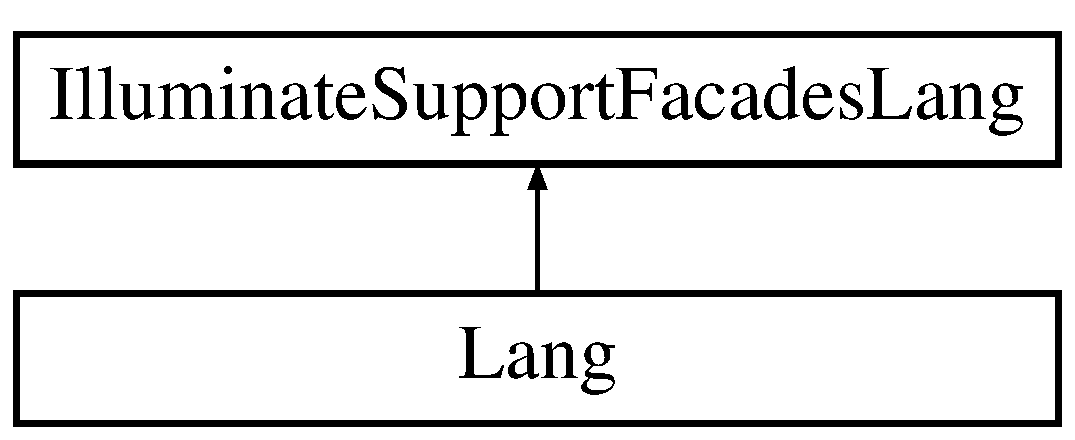
\includegraphics[height=2.000000cm]{class_lang}
\end{center}
\end{figure}
\subsection*{Additional Inherited Members}


The documentation for this class was generated from the following file\+:\begin{DoxyCompactItemize}
\item 
\+\_\+ide\+\_\+helper.\+php\end{DoxyCompactItemize}

\hypertarget{class_illuminate_1_1_support_1_1_facades_1_1_log}{}\section{Illuminate\textbackslash{}Support\textbackslash{}Facades\textbackslash{}Log Class Reference}
\label{class_illuminate_1_1_support_1_1_facades_1_1_log}\index{Illuminate\textbackslash{}\+Support\textbackslash{}\+Facades\textbackslash{}\+Log@{Illuminate\textbackslash{}\+Support\textbackslash{}\+Facades\textbackslash{}\+Log}}
Inheritance diagram for Illuminate\textbackslash{}Support\textbackslash{}Facades\textbackslash{}Log\+:\begin{figure}[H]
\begin{center}
\leavevmode
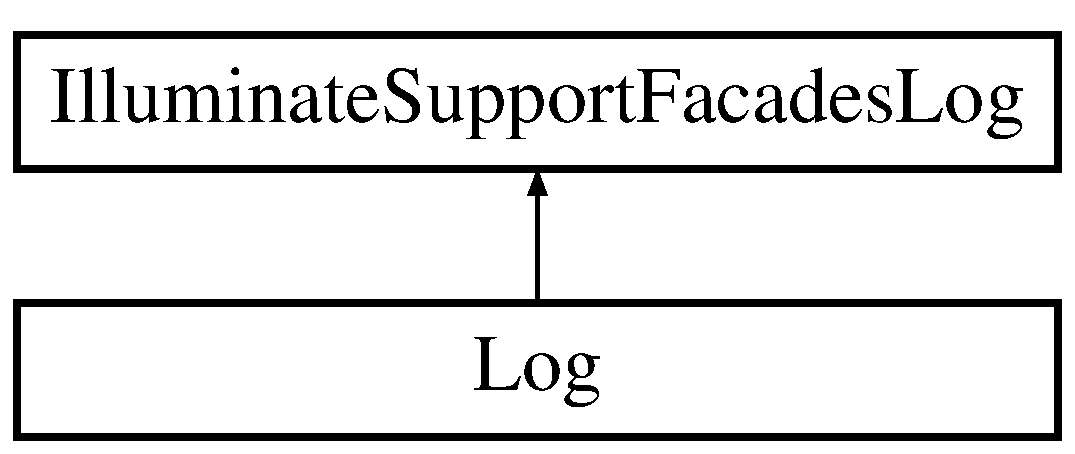
\includegraphics[height=2.000000cm]{class_illuminate_1_1_support_1_1_facades_1_1_log}
\end{center}
\end{figure}
\subsection*{Static Public Member Functions}
\begin{DoxyCompactItemize}
\item 
static \mbox{\hyperlink{class_illuminate_1_1_support_1_1_facades_1_1_log_a4a6186c4b8318f3096e043e59a2683f8}{debug}} (\$message, \$context=array())
\item 
static \mbox{\hyperlink{class_illuminate_1_1_support_1_1_facades_1_1_log_acbbeebd340cccb5b259b123086d962d3}{info}} (\$message, \$context=array())
\item 
static \mbox{\hyperlink{class_illuminate_1_1_support_1_1_facades_1_1_log_a763d78ea6e79ac04371d3c2e59470b9b}{notice}} (\$message, \$context=array())
\item 
static \mbox{\hyperlink{class_illuminate_1_1_support_1_1_facades_1_1_log_a48aba756d59b9b8ad7be5d67e5ea0860}{warning}} (\$message, \$context=array())
\item 
static \mbox{\hyperlink{class_illuminate_1_1_support_1_1_facades_1_1_log_aef174a11b64b8e9c5ed1ba6cc8e5bb4a}{error}} (\$message, \$context=array())
\item 
static \mbox{\hyperlink{class_illuminate_1_1_support_1_1_facades_1_1_log_a2f93306eee277c10de13357087185b17}{critical}} (\$message, \$context=array())
\item 
static \mbox{\hyperlink{class_illuminate_1_1_support_1_1_facades_1_1_log_a65867128ee36796382e33c5546f18aae}{alert}} (\$message, \$context=array())
\item 
static \mbox{\hyperlink{class_illuminate_1_1_support_1_1_facades_1_1_log_a5da3678ba016f92e8c882a7adf1ca9e4}{emergency}} (\$message, \$context=array())
\item 
static \mbox{\hyperlink{class_illuminate_1_1_support_1_1_facades_1_1_log_a3b7d90ecb5892e00e9f4fed096cef427}{log}} (\$level, \$message, \$context=array())
\item 
static \mbox{\hyperlink{class_illuminate_1_1_support_1_1_facades_1_1_log_ac215cf462c16fdc847eea15bd760690e}{write}} (\$level, \$message, \$context=array())
\item 
static \mbox{\hyperlink{class_illuminate_1_1_support_1_1_facades_1_1_log_a498cc17d8075089609bf0875887d5a50}{use\+Files}} (\$path, \$level=\textquotesingle{}\mbox{\hyperlink{class_illuminate_1_1_support_1_1_facades_1_1_log_a4a6186c4b8318f3096e043e59a2683f8}{debug}}\textquotesingle{})
\item 
static \mbox{\hyperlink{class_illuminate_1_1_support_1_1_facades_1_1_log_a13cb363de24b3c76b32460c18e1a99d1}{use\+Daily\+Files}} (\$path, \$days=0, \$level=\textquotesingle{}\mbox{\hyperlink{class_illuminate_1_1_support_1_1_facades_1_1_log_a4a6186c4b8318f3096e043e59a2683f8}{debug}}\textquotesingle{})
\item 
static \mbox{\hyperlink{class_illuminate_1_1_support_1_1_facades_1_1_log_a351af1020b92d8bbd8fa6179234a27f4}{use\+Syslog}} (\$name=\textquotesingle{}laravel\textquotesingle{}, \$level=\textquotesingle{}\mbox{\hyperlink{class_illuminate_1_1_support_1_1_facades_1_1_log_a4a6186c4b8318f3096e043e59a2683f8}{debug}}\textquotesingle{}, \$facility=8)
\item 
static \mbox{\hyperlink{class_illuminate_1_1_support_1_1_facades_1_1_log_a703c784c074caa43b7b68579e609fa48}{use\+Error\+Log}} (\$level=\textquotesingle{}\mbox{\hyperlink{class_illuminate_1_1_support_1_1_facades_1_1_log_a4a6186c4b8318f3096e043e59a2683f8}{debug}}\textquotesingle{}, \$message\+Type=0)
\item 
static \mbox{\hyperlink{class_illuminate_1_1_support_1_1_facades_1_1_log_a7df6ff6379ae011b0ad9db602ceae2b6}{listen}} (\$callback)
\item 
static \mbox{\hyperlink{class_illuminate_1_1_support_1_1_facades_1_1_log_a0c00c7c59ce5ce04e3ed5f29e17788ab}{get\+Monolog}} ()
\item 
static \mbox{\hyperlink{class_illuminate_1_1_support_1_1_facades_1_1_log_a1006c5d64b4b975b55efb6c11ec0b3c8}{get\+Event\+Dispatcher}} ()
\item 
static \mbox{\hyperlink{class_illuminate_1_1_support_1_1_facades_1_1_log_adf269d76df35f73950371f4432804e38}{set\+Event\+Dispatcher}} (\$dispatcher)
\end{DoxyCompactItemize}


\subsection{Member Function Documentation}
\mbox{\Hypertarget{class_illuminate_1_1_support_1_1_facades_1_1_log_a65867128ee36796382e33c5546f18aae}\label{class_illuminate_1_1_support_1_1_facades_1_1_log_a65867128ee36796382e33c5546f18aae}} 
\index{Illuminate\+::\+Support\+::\+Facades\+::\+Log@{Illuminate\+::\+Support\+::\+Facades\+::\+Log}!alert@{alert}}
\index{alert@{alert}!Illuminate\+::\+Support\+::\+Facades\+::\+Log@{Illuminate\+::\+Support\+::\+Facades\+::\+Log}}
\subsubsection{\texorpdfstring{alert()}{alert()}}
{\footnotesize\ttfamily static Illuminate\textbackslash{}\+Support\textbackslash{}\+Facades\textbackslash{}\+Log\+::alert (\begin{DoxyParamCaption}\item[{}]{\$message,  }\item[{}]{\$context = {\ttfamily array()} }\end{DoxyParamCaption})\hspace{0.3cm}{\ttfamily [static]}}

Adds a log record at the A\+L\+E\+RT level.


\begin{DoxyParams}[1]{Parameters}
string & {\em \$message} & The log message \\
\hline
array & {\em \$context} & The log context \\
\hline
\end{DoxyParams}
\begin{DoxyReturn}{Returns}
Boolean Whether the record has been processed 
\end{DoxyReturn}
\mbox{\Hypertarget{class_illuminate_1_1_support_1_1_facades_1_1_log_a2f93306eee277c10de13357087185b17}\label{class_illuminate_1_1_support_1_1_facades_1_1_log_a2f93306eee277c10de13357087185b17}} 
\index{Illuminate\+::\+Support\+::\+Facades\+::\+Log@{Illuminate\+::\+Support\+::\+Facades\+::\+Log}!critical@{critical}}
\index{critical@{critical}!Illuminate\+::\+Support\+::\+Facades\+::\+Log@{Illuminate\+::\+Support\+::\+Facades\+::\+Log}}
\subsubsection{\texorpdfstring{critical()}{critical()}}
{\footnotesize\ttfamily static Illuminate\textbackslash{}\+Support\textbackslash{}\+Facades\textbackslash{}\+Log\+::critical (\begin{DoxyParamCaption}\item[{}]{\$message,  }\item[{}]{\$context = {\ttfamily array()} }\end{DoxyParamCaption})\hspace{0.3cm}{\ttfamily [static]}}

Adds a log record at the C\+R\+I\+T\+I\+C\+AL level.


\begin{DoxyParams}[1]{Parameters}
string & {\em \$message} & The log message \\
\hline
array & {\em \$context} & The log context \\
\hline
\end{DoxyParams}
\begin{DoxyReturn}{Returns}
Boolean Whether the record has been processed 
\end{DoxyReturn}
\mbox{\Hypertarget{class_illuminate_1_1_support_1_1_facades_1_1_log_a4a6186c4b8318f3096e043e59a2683f8}\label{class_illuminate_1_1_support_1_1_facades_1_1_log_a4a6186c4b8318f3096e043e59a2683f8}} 
\index{Illuminate\+::\+Support\+::\+Facades\+::\+Log@{Illuminate\+::\+Support\+::\+Facades\+::\+Log}!debug@{debug}}
\index{debug@{debug}!Illuminate\+::\+Support\+::\+Facades\+::\+Log@{Illuminate\+::\+Support\+::\+Facades\+::\+Log}}
\subsubsection{\texorpdfstring{debug()}{debug()}}
{\footnotesize\ttfamily static Illuminate\textbackslash{}\+Support\textbackslash{}\+Facades\textbackslash{}\+Log\+::debug (\begin{DoxyParamCaption}\item[{}]{\$message,  }\item[{}]{\$context = {\ttfamily array()} }\end{DoxyParamCaption})\hspace{0.3cm}{\ttfamily [static]}}

Adds a log record at the D\+E\+B\+UG level.


\begin{DoxyParams}[1]{Parameters}
string & {\em \$message} & The log message \\
\hline
array & {\em \$context} & The log context \\
\hline
\end{DoxyParams}
\begin{DoxyReturn}{Returns}
Boolean Whether the record has been processed 
\end{DoxyReturn}
\mbox{\Hypertarget{class_illuminate_1_1_support_1_1_facades_1_1_log_a5da3678ba016f92e8c882a7adf1ca9e4}\label{class_illuminate_1_1_support_1_1_facades_1_1_log_a5da3678ba016f92e8c882a7adf1ca9e4}} 
\index{Illuminate\+::\+Support\+::\+Facades\+::\+Log@{Illuminate\+::\+Support\+::\+Facades\+::\+Log}!emergency@{emergency}}
\index{emergency@{emergency}!Illuminate\+::\+Support\+::\+Facades\+::\+Log@{Illuminate\+::\+Support\+::\+Facades\+::\+Log}}
\subsubsection{\texorpdfstring{emergency()}{emergency()}}
{\footnotesize\ttfamily static Illuminate\textbackslash{}\+Support\textbackslash{}\+Facades\textbackslash{}\+Log\+::emergency (\begin{DoxyParamCaption}\item[{}]{\$message,  }\item[{}]{\$context = {\ttfamily array()} }\end{DoxyParamCaption})\hspace{0.3cm}{\ttfamily [static]}}

Adds a log record at the E\+M\+E\+R\+G\+E\+N\+CY level.


\begin{DoxyParams}[1]{Parameters}
string & {\em \$message} & The log message \\
\hline
array & {\em \$context} & The log context \\
\hline
\end{DoxyParams}
\begin{DoxyReturn}{Returns}
Boolean Whether the record has been processed 
\end{DoxyReturn}
\mbox{\Hypertarget{class_illuminate_1_1_support_1_1_facades_1_1_log_aef174a11b64b8e9c5ed1ba6cc8e5bb4a}\label{class_illuminate_1_1_support_1_1_facades_1_1_log_aef174a11b64b8e9c5ed1ba6cc8e5bb4a}} 
\index{Illuminate\+::\+Support\+::\+Facades\+::\+Log@{Illuminate\+::\+Support\+::\+Facades\+::\+Log}!error@{error}}
\index{error@{error}!Illuminate\+::\+Support\+::\+Facades\+::\+Log@{Illuminate\+::\+Support\+::\+Facades\+::\+Log}}
\subsubsection{\texorpdfstring{error()}{error()}}
{\footnotesize\ttfamily static Illuminate\textbackslash{}\+Support\textbackslash{}\+Facades\textbackslash{}\+Log\+::error (\begin{DoxyParamCaption}\item[{}]{\$message,  }\item[{}]{\$context = {\ttfamily array()} }\end{DoxyParamCaption})\hspace{0.3cm}{\ttfamily [static]}}

Adds a log record at the E\+R\+R\+OR level.


\begin{DoxyParams}[1]{Parameters}
string & {\em \$message} & The log message \\
\hline
array & {\em \$context} & The log context \\
\hline
\end{DoxyParams}
\begin{DoxyReturn}{Returns}
Boolean Whether the record has been processed 
\end{DoxyReturn}
\mbox{\Hypertarget{class_illuminate_1_1_support_1_1_facades_1_1_log_a1006c5d64b4b975b55efb6c11ec0b3c8}\label{class_illuminate_1_1_support_1_1_facades_1_1_log_a1006c5d64b4b975b55efb6c11ec0b3c8}} 
\index{Illuminate\+::\+Support\+::\+Facades\+::\+Log@{Illuminate\+::\+Support\+::\+Facades\+::\+Log}!get\+Event\+Dispatcher@{get\+Event\+Dispatcher}}
\index{get\+Event\+Dispatcher@{get\+Event\+Dispatcher}!Illuminate\+::\+Support\+::\+Facades\+::\+Log@{Illuminate\+::\+Support\+::\+Facades\+::\+Log}}
\subsubsection{\texorpdfstring{get\+Event\+Dispatcher()}{getEventDispatcher()}}
{\footnotesize\ttfamily static Illuminate\textbackslash{}\+Support\textbackslash{}\+Facades\textbackslash{}\+Log\+::get\+Event\+Dispatcher (\begin{DoxyParamCaption}{ }\end{DoxyParamCaption})\hspace{0.3cm}{\ttfamily [static]}}

Get the event dispatcher instance.

\begin{DoxyReturn}{Returns}

\end{DoxyReturn}
\mbox{\Hypertarget{class_illuminate_1_1_support_1_1_facades_1_1_log_a0c00c7c59ce5ce04e3ed5f29e17788ab}\label{class_illuminate_1_1_support_1_1_facades_1_1_log_a0c00c7c59ce5ce04e3ed5f29e17788ab}} 
\index{Illuminate\+::\+Support\+::\+Facades\+::\+Log@{Illuminate\+::\+Support\+::\+Facades\+::\+Log}!get\+Monolog@{get\+Monolog}}
\index{get\+Monolog@{get\+Monolog}!Illuminate\+::\+Support\+::\+Facades\+::\+Log@{Illuminate\+::\+Support\+::\+Facades\+::\+Log}}
\subsubsection{\texorpdfstring{get\+Monolog()}{getMonolog()}}
{\footnotesize\ttfamily static Illuminate\textbackslash{}\+Support\textbackslash{}\+Facades\textbackslash{}\+Log\+::get\+Monolog (\begin{DoxyParamCaption}{ }\end{DoxyParamCaption})\hspace{0.3cm}{\ttfamily [static]}}

Get the underlying Monolog instance.

\begin{DoxyReturn}{Returns}

\end{DoxyReturn}
\mbox{\Hypertarget{class_illuminate_1_1_support_1_1_facades_1_1_log_acbbeebd340cccb5b259b123086d962d3}\label{class_illuminate_1_1_support_1_1_facades_1_1_log_acbbeebd340cccb5b259b123086d962d3}} 
\index{Illuminate\+::\+Support\+::\+Facades\+::\+Log@{Illuminate\+::\+Support\+::\+Facades\+::\+Log}!info@{info}}
\index{info@{info}!Illuminate\+::\+Support\+::\+Facades\+::\+Log@{Illuminate\+::\+Support\+::\+Facades\+::\+Log}}
\subsubsection{\texorpdfstring{info()}{info()}}
{\footnotesize\ttfamily static Illuminate\textbackslash{}\+Support\textbackslash{}\+Facades\textbackslash{}\+Log\+::info (\begin{DoxyParamCaption}\item[{}]{\$message,  }\item[{}]{\$context = {\ttfamily array()} }\end{DoxyParamCaption})\hspace{0.3cm}{\ttfamily [static]}}

Adds a log record at the I\+N\+FO level.


\begin{DoxyParams}[1]{Parameters}
string & {\em \$message} & The log message \\
\hline
array & {\em \$context} & The log context \\
\hline
\end{DoxyParams}
\begin{DoxyReturn}{Returns}
Boolean Whether the record has been processed 
\end{DoxyReturn}
\mbox{\Hypertarget{class_illuminate_1_1_support_1_1_facades_1_1_log_a7df6ff6379ae011b0ad9db602ceae2b6}\label{class_illuminate_1_1_support_1_1_facades_1_1_log_a7df6ff6379ae011b0ad9db602ceae2b6}} 
\index{Illuminate\+::\+Support\+::\+Facades\+::\+Log@{Illuminate\+::\+Support\+::\+Facades\+::\+Log}!listen@{listen}}
\index{listen@{listen}!Illuminate\+::\+Support\+::\+Facades\+::\+Log@{Illuminate\+::\+Support\+::\+Facades\+::\+Log}}
\subsubsection{\texorpdfstring{listen()}{listen()}}
{\footnotesize\ttfamily static Illuminate\textbackslash{}\+Support\textbackslash{}\+Facades\textbackslash{}\+Log\+::listen (\begin{DoxyParamCaption}\item[{}]{\$callback }\end{DoxyParamCaption})\hspace{0.3cm}{\ttfamily [static]}}

Register a new callback handler for when a log event is triggered.


\begin{DoxyParams}[1]{Parameters}
\textbackslash{}\+Closure & {\em \$callback} & \\
\hline
\end{DoxyParams}
\begin{DoxyReturn}{Returns}
void 
\end{DoxyReturn}

\begin{DoxyExceptions}{Exceptions}
{\em } & \\
\hline
\end{DoxyExceptions}
\mbox{\Hypertarget{class_illuminate_1_1_support_1_1_facades_1_1_log_a3b7d90ecb5892e00e9f4fed096cef427}\label{class_illuminate_1_1_support_1_1_facades_1_1_log_a3b7d90ecb5892e00e9f4fed096cef427}} 
\index{Illuminate\+::\+Support\+::\+Facades\+::\+Log@{Illuminate\+::\+Support\+::\+Facades\+::\+Log}!log@{log}}
\index{log@{log}!Illuminate\+::\+Support\+::\+Facades\+::\+Log@{Illuminate\+::\+Support\+::\+Facades\+::\+Log}}
\subsubsection{\texorpdfstring{log()}{log()}}
{\footnotesize\ttfamily static Illuminate\textbackslash{}\+Support\textbackslash{}\+Facades\textbackslash{}\+Log\+::log (\begin{DoxyParamCaption}\item[{}]{\$level,  }\item[{}]{\$message,  }\item[{}]{\$context = {\ttfamily array()} }\end{DoxyParamCaption})\hspace{0.3cm}{\ttfamily [static]}}

\mbox{\hyperlink{class_illuminate_1_1_support_1_1_facades_1_1_log}{Log}} a message to the logs.


\begin{DoxyParams}[1]{Parameters}
string & {\em \$level} & \\
\hline
string & {\em \$message} & \\
\hline
array & {\em \$context} & \\
\hline
\end{DoxyParams}
\begin{DoxyReturn}{Returns}
void 
\end{DoxyReturn}
\mbox{\Hypertarget{class_illuminate_1_1_support_1_1_facades_1_1_log_a763d78ea6e79ac04371d3c2e59470b9b}\label{class_illuminate_1_1_support_1_1_facades_1_1_log_a763d78ea6e79ac04371d3c2e59470b9b}} 
\index{Illuminate\+::\+Support\+::\+Facades\+::\+Log@{Illuminate\+::\+Support\+::\+Facades\+::\+Log}!notice@{notice}}
\index{notice@{notice}!Illuminate\+::\+Support\+::\+Facades\+::\+Log@{Illuminate\+::\+Support\+::\+Facades\+::\+Log}}
\subsubsection{\texorpdfstring{notice()}{notice()}}
{\footnotesize\ttfamily static Illuminate\textbackslash{}\+Support\textbackslash{}\+Facades\textbackslash{}\+Log\+::notice (\begin{DoxyParamCaption}\item[{}]{\$message,  }\item[{}]{\$context = {\ttfamily array()} }\end{DoxyParamCaption})\hspace{0.3cm}{\ttfamily [static]}}

Adds a log record at the N\+O\+T\+I\+CE level.


\begin{DoxyParams}[1]{Parameters}
string & {\em \$message} & The log message \\
\hline
array & {\em \$context} & The log context \\
\hline
\end{DoxyParams}
\begin{DoxyReturn}{Returns}
Boolean Whether the record has been processed 
\end{DoxyReturn}
\mbox{\Hypertarget{class_illuminate_1_1_support_1_1_facades_1_1_log_adf269d76df35f73950371f4432804e38}\label{class_illuminate_1_1_support_1_1_facades_1_1_log_adf269d76df35f73950371f4432804e38}} 
\index{Illuminate\+::\+Support\+::\+Facades\+::\+Log@{Illuminate\+::\+Support\+::\+Facades\+::\+Log}!set\+Event\+Dispatcher@{set\+Event\+Dispatcher}}
\index{set\+Event\+Dispatcher@{set\+Event\+Dispatcher}!Illuminate\+::\+Support\+::\+Facades\+::\+Log@{Illuminate\+::\+Support\+::\+Facades\+::\+Log}}
\subsubsection{\texorpdfstring{set\+Event\+Dispatcher()}{setEventDispatcher()}}
{\footnotesize\ttfamily static Illuminate\textbackslash{}\+Support\textbackslash{}\+Facades\textbackslash{}\+Log\+::set\+Event\+Dispatcher (\begin{DoxyParamCaption}\item[{}]{\$dispatcher }\end{DoxyParamCaption})\hspace{0.3cm}{\ttfamily [static]}}

Set the event dispatcher instance.


\begin{DoxyParams}[1]{Parameters}
\textbackslash{}\+Illuminate\textbackslash{}\+Contracts\textbackslash{}\+Events\textbackslash{}\+Dispatcher & {\em \$dispatcher} & \\
\hline
\end{DoxyParams}
\begin{DoxyReturn}{Returns}
void 
\end{DoxyReturn}
\mbox{\Hypertarget{class_illuminate_1_1_support_1_1_facades_1_1_log_a13cb363de24b3c76b32460c18e1a99d1}\label{class_illuminate_1_1_support_1_1_facades_1_1_log_a13cb363de24b3c76b32460c18e1a99d1}} 
\index{Illuminate\+::\+Support\+::\+Facades\+::\+Log@{Illuminate\+::\+Support\+::\+Facades\+::\+Log}!use\+Daily\+Files@{use\+Daily\+Files}}
\index{use\+Daily\+Files@{use\+Daily\+Files}!Illuminate\+::\+Support\+::\+Facades\+::\+Log@{Illuminate\+::\+Support\+::\+Facades\+::\+Log}}
\subsubsection{\texorpdfstring{use\+Daily\+Files()}{useDailyFiles()}}
{\footnotesize\ttfamily static Illuminate\textbackslash{}\+Support\textbackslash{}\+Facades\textbackslash{}\+Log\+::use\+Daily\+Files (\begin{DoxyParamCaption}\item[{}]{\$path,  }\item[{}]{\$days = {\ttfamily 0},  }\item[{}]{\$level = {\ttfamily \textquotesingle{}\mbox{\hyperlink{class_illuminate_1_1_support_1_1_facades_1_1_log_a4a6186c4b8318f3096e043e59a2683f8}{debug}}\textquotesingle{}} }\end{DoxyParamCaption})\hspace{0.3cm}{\ttfamily [static]}}

Register a daily file log handler.


\begin{DoxyParams}[1]{Parameters}
string & {\em \$path} & \\
\hline
int & {\em \$days} & \\
\hline
string & {\em \$level} & \\
\hline
\end{DoxyParams}
\begin{DoxyReturn}{Returns}
void 
\end{DoxyReturn}
\mbox{\Hypertarget{class_illuminate_1_1_support_1_1_facades_1_1_log_a703c784c074caa43b7b68579e609fa48}\label{class_illuminate_1_1_support_1_1_facades_1_1_log_a703c784c074caa43b7b68579e609fa48}} 
\index{Illuminate\+::\+Support\+::\+Facades\+::\+Log@{Illuminate\+::\+Support\+::\+Facades\+::\+Log}!use\+Error\+Log@{use\+Error\+Log}}
\index{use\+Error\+Log@{use\+Error\+Log}!Illuminate\+::\+Support\+::\+Facades\+::\+Log@{Illuminate\+::\+Support\+::\+Facades\+::\+Log}}
\subsubsection{\texorpdfstring{use\+Error\+Log()}{useErrorLog()}}
{\footnotesize\ttfamily static Illuminate\textbackslash{}\+Support\textbackslash{}\+Facades\textbackslash{}\+Log\+::use\+Error\+Log (\begin{DoxyParamCaption}\item[{}]{\$level = {\ttfamily \textquotesingle{}\mbox{\hyperlink{class_illuminate_1_1_support_1_1_facades_1_1_log_a4a6186c4b8318f3096e043e59a2683f8}{debug}}\textquotesingle{}},  }\item[{}]{\$message\+Type = {\ttfamily 0} }\end{DoxyParamCaption})\hspace{0.3cm}{\ttfamily [static]}}

Register an error\+\_\+log handler.


\begin{DoxyParams}[1]{Parameters}
string & {\em \$level} & \\
\hline
int & {\em \$message\+Type} & \\
\hline
\end{DoxyParams}
\begin{DoxyReturn}{Returns}
void 
\end{DoxyReturn}
\mbox{\Hypertarget{class_illuminate_1_1_support_1_1_facades_1_1_log_a498cc17d8075089609bf0875887d5a50}\label{class_illuminate_1_1_support_1_1_facades_1_1_log_a498cc17d8075089609bf0875887d5a50}} 
\index{Illuminate\+::\+Support\+::\+Facades\+::\+Log@{Illuminate\+::\+Support\+::\+Facades\+::\+Log}!use\+Files@{use\+Files}}
\index{use\+Files@{use\+Files}!Illuminate\+::\+Support\+::\+Facades\+::\+Log@{Illuminate\+::\+Support\+::\+Facades\+::\+Log}}
\subsubsection{\texorpdfstring{use\+Files()}{useFiles()}}
{\footnotesize\ttfamily static Illuminate\textbackslash{}\+Support\textbackslash{}\+Facades\textbackslash{}\+Log\+::use\+Files (\begin{DoxyParamCaption}\item[{}]{\$path,  }\item[{}]{\$level = {\ttfamily \textquotesingle{}\mbox{\hyperlink{class_illuminate_1_1_support_1_1_facades_1_1_log_a4a6186c4b8318f3096e043e59a2683f8}{debug}}\textquotesingle{}} }\end{DoxyParamCaption})\hspace{0.3cm}{\ttfamily [static]}}

Register a file log handler.


\begin{DoxyParams}[1]{Parameters}
string & {\em \$path} & \\
\hline
string & {\em \$level} & \\
\hline
\end{DoxyParams}
\begin{DoxyReturn}{Returns}
void 
\end{DoxyReturn}
\mbox{\Hypertarget{class_illuminate_1_1_support_1_1_facades_1_1_log_a351af1020b92d8bbd8fa6179234a27f4}\label{class_illuminate_1_1_support_1_1_facades_1_1_log_a351af1020b92d8bbd8fa6179234a27f4}} 
\index{Illuminate\+::\+Support\+::\+Facades\+::\+Log@{Illuminate\+::\+Support\+::\+Facades\+::\+Log}!use\+Syslog@{use\+Syslog}}
\index{use\+Syslog@{use\+Syslog}!Illuminate\+::\+Support\+::\+Facades\+::\+Log@{Illuminate\+::\+Support\+::\+Facades\+::\+Log}}
\subsubsection{\texorpdfstring{use\+Syslog()}{useSyslog()}}
{\footnotesize\ttfamily static Illuminate\textbackslash{}\+Support\textbackslash{}\+Facades\textbackslash{}\+Log\+::use\+Syslog (\begin{DoxyParamCaption}\item[{}]{\$name = {\ttfamily \textquotesingle{}laravel\textquotesingle{}},  }\item[{}]{\$level = {\ttfamily \textquotesingle{}\mbox{\hyperlink{class_illuminate_1_1_support_1_1_facades_1_1_log_a4a6186c4b8318f3096e043e59a2683f8}{debug}}\textquotesingle{}},  }\item[{}]{\$facility = {\ttfamily 8} }\end{DoxyParamCaption})\hspace{0.3cm}{\ttfamily [static]}}

Register a Syslog handler.


\begin{DoxyParams}[1]{Parameters}
string & {\em \$name} & \\
\hline
string & {\em \$level} & \\
\hline
mixed & {\em \$facility} & \\
\hline
\end{DoxyParams}
\begin{DoxyReturn}{Returns}

\end{DoxyReturn}
\mbox{\Hypertarget{class_illuminate_1_1_support_1_1_facades_1_1_log_a48aba756d59b9b8ad7be5d67e5ea0860}\label{class_illuminate_1_1_support_1_1_facades_1_1_log_a48aba756d59b9b8ad7be5d67e5ea0860}} 
\index{Illuminate\+::\+Support\+::\+Facades\+::\+Log@{Illuminate\+::\+Support\+::\+Facades\+::\+Log}!warning@{warning}}
\index{warning@{warning}!Illuminate\+::\+Support\+::\+Facades\+::\+Log@{Illuminate\+::\+Support\+::\+Facades\+::\+Log}}
\subsubsection{\texorpdfstring{warning()}{warning()}}
{\footnotesize\ttfamily static Illuminate\textbackslash{}\+Support\textbackslash{}\+Facades\textbackslash{}\+Log\+::warning (\begin{DoxyParamCaption}\item[{}]{\$message,  }\item[{}]{\$context = {\ttfamily array()} }\end{DoxyParamCaption})\hspace{0.3cm}{\ttfamily [static]}}

Adds a log record at the W\+A\+R\+N\+I\+NG level.


\begin{DoxyParams}[1]{Parameters}
string & {\em \$message} & The log message \\
\hline
array & {\em \$context} & The log context \\
\hline
\end{DoxyParams}
\begin{DoxyReturn}{Returns}
Boolean Whether the record has been processed 
\end{DoxyReturn}
\mbox{\Hypertarget{class_illuminate_1_1_support_1_1_facades_1_1_log_ac215cf462c16fdc847eea15bd760690e}\label{class_illuminate_1_1_support_1_1_facades_1_1_log_ac215cf462c16fdc847eea15bd760690e}} 
\index{Illuminate\+::\+Support\+::\+Facades\+::\+Log@{Illuminate\+::\+Support\+::\+Facades\+::\+Log}!write@{write}}
\index{write@{write}!Illuminate\+::\+Support\+::\+Facades\+::\+Log@{Illuminate\+::\+Support\+::\+Facades\+::\+Log}}
\subsubsection{\texorpdfstring{write()}{write()}}
{\footnotesize\ttfamily static Illuminate\textbackslash{}\+Support\textbackslash{}\+Facades\textbackslash{}\+Log\+::write (\begin{DoxyParamCaption}\item[{}]{\$level,  }\item[{}]{\$message,  }\item[{}]{\$context = {\ttfamily array()} }\end{DoxyParamCaption})\hspace{0.3cm}{\ttfamily [static]}}

Dynamically pass log calls into the writer.


\begin{DoxyParams}[1]{Parameters}
string & {\em \$level} & \\
\hline
string & {\em \$message} & \\
\hline
array & {\em \$context} & \\
\hline
\end{DoxyParams}
\begin{DoxyReturn}{Returns}
void 
\end{DoxyReturn}


The documentation for this class was generated from the following file\+:\begin{DoxyCompactItemize}
\item 
\+\_\+ide\+\_\+helper.\+php\end{DoxyCompactItemize}

\hypertarget{class_log}{}\section{Log Class Reference}
\label{class_log}\index{Log@{Log}}
Inheritance diagram for Log\+:\begin{figure}[H]
\begin{center}
\leavevmode
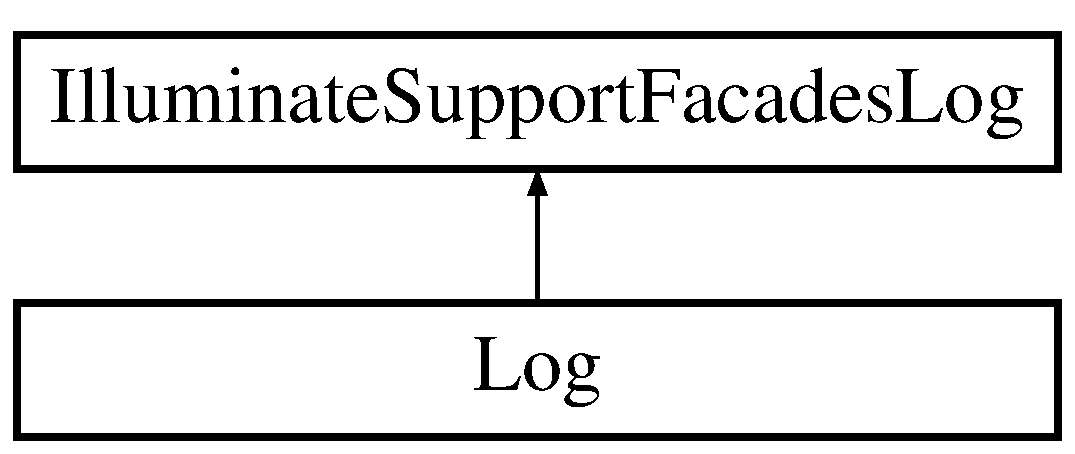
\includegraphics[height=2.000000cm]{class_log}
\end{center}
\end{figure}
\subsection*{Additional Inherited Members}


The documentation for this class was generated from the following file\+:\begin{DoxyCompactItemize}
\item 
\+\_\+ide\+\_\+helper.\+php\end{DoxyCompactItemize}

\hypertarget{class_illuminate_1_1_support_1_1_facades_1_1_mail}{}\section{Illuminate\textbackslash{}Support\textbackslash{}Facades\textbackslash{}Mail Class Reference}
\label{class_illuminate_1_1_support_1_1_facades_1_1_mail}\index{Illuminate\textbackslash{}\+Support\textbackslash{}\+Facades\textbackslash{}\+Mail@{Illuminate\textbackslash{}\+Support\textbackslash{}\+Facades\textbackslash{}\+Mail}}
Inheritance diagram for Illuminate\textbackslash{}Support\textbackslash{}Facades\textbackslash{}Mail\+:\begin{figure}[H]
\begin{center}
\leavevmode
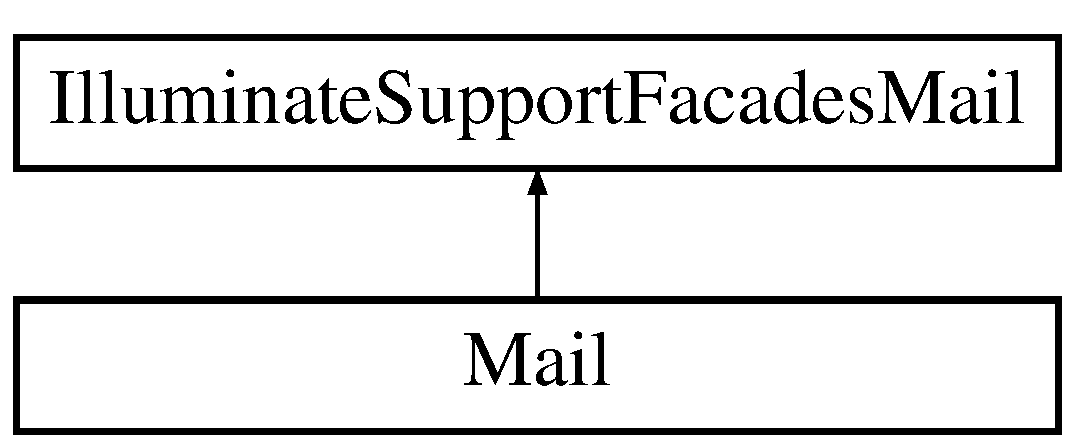
\includegraphics[height=2.000000cm]{class_illuminate_1_1_support_1_1_facades_1_1_mail}
\end{center}
\end{figure}
\subsection*{Static Public Member Functions}
\begin{DoxyCompactItemize}
\item 
static \mbox{\hyperlink{class_illuminate_1_1_support_1_1_facades_1_1_mail_a24a500e68752fd86d4d2ad057431f3d7}{always\+From}} (\$address, \$name=null)
\item 
static \mbox{\hyperlink{class_illuminate_1_1_support_1_1_facades_1_1_mail_a65ebb2e9119b6764ebc06d7902759e68}{always\+Reply\+To}} (\$address, \$name=null)
\item 
static \mbox{\hyperlink{class_illuminate_1_1_support_1_1_facades_1_1_mail_a83714f3037e20389411b8274e3ed681a}{always\+To}} (\$address, \$name=null)
\item 
static \mbox{\hyperlink{class_illuminate_1_1_support_1_1_facades_1_1_mail_afbe8a912037dc180cfbd366144eb3a1f}{to}} (\$users)
\item 
static \mbox{\hyperlink{class_illuminate_1_1_support_1_1_facades_1_1_mail_a6bdd27b91af1bcea3fbf014dbd1127ef}{bcc}} (\$users)
\item 
static \mbox{\hyperlink{class_illuminate_1_1_support_1_1_facades_1_1_mail_a4dc9b81bde1bfd5b77ee735a6a09770d}{raw}} (\$text, \$callback)
\item 
static \mbox{\hyperlink{class_illuminate_1_1_support_1_1_facades_1_1_mail_ac99a987ce3f8cc915099da60b9fcaac4}{plain}} (\$view, \$data, \$callback)
\item 
static \mbox{\hyperlink{class_illuminate_1_1_support_1_1_facades_1_1_mail_a4f143bb75a63e5b82474608d754fce45}{render}} (\$view, \$data=array())
\item 
static \mbox{\hyperlink{class_illuminate_1_1_support_1_1_facades_1_1_mail_a700308972c34fae3fda5535834aa43de}{send}} (\$view, \$data=array(), \$callback=null)
\item 
static \mbox{\hyperlink{class_illuminate_1_1_support_1_1_facades_1_1_mail_a478836272e2433d16e0b02f850e146ac}{queue}} (\$view, \$queue=null)
\item 
static \mbox{\hyperlink{class_illuminate_1_1_support_1_1_facades_1_1_mail_a48e157639b1432f6bcc5e3a8ec2cd5e1}{on\+Queue}} (\$\mbox{\hyperlink{class_illuminate_1_1_support_1_1_facades_1_1_mail_a478836272e2433d16e0b02f850e146ac}{queue}}, \$view)
\item 
static \mbox{\hyperlink{class_illuminate_1_1_support_1_1_facades_1_1_mail_ae508af6b2c70a392a70ec240e43dad50}{queue\+On}} (\$\mbox{\hyperlink{class_illuminate_1_1_support_1_1_facades_1_1_mail_a478836272e2433d16e0b02f850e146ac}{queue}}, \$view)
\item 
static \mbox{\hyperlink{class_illuminate_1_1_support_1_1_facades_1_1_mail_a2972059488d1ba83e8acc56cabc269f0}{later}} (\$delay, \$view, \$\mbox{\hyperlink{class_illuminate_1_1_support_1_1_facades_1_1_mail_a478836272e2433d16e0b02f850e146ac}{queue}}=null)
\item 
static \mbox{\hyperlink{class_illuminate_1_1_support_1_1_facades_1_1_mail_a1247d0e81905df819e8e3e015917128c}{later\+On}} (\$\mbox{\hyperlink{class_illuminate_1_1_support_1_1_facades_1_1_mail_a478836272e2433d16e0b02f850e146ac}{queue}}, \$delay, \$view)
\item 
static \mbox{\hyperlink{class_illuminate_1_1_support_1_1_facades_1_1_mail_a4e55d12d552d180f8c4684c31debed90}{get\+View\+Factory}} ()
\item 
static \mbox{\hyperlink{class_illuminate_1_1_support_1_1_facades_1_1_mail_a1e36e3a729e3286f8d5e531c74685eb6}{get\+Swift\+Mailer}} ()
\item 
static \mbox{\hyperlink{class_illuminate_1_1_support_1_1_facades_1_1_mail_abf36e9099d5512f43e32522e871d2ecd}{failures}} ()
\item 
static \mbox{\hyperlink{class_illuminate_1_1_support_1_1_facades_1_1_mail_a3350fe2ac5cd333f571c105dcf372dcb}{set\+Swift\+Mailer}} (\$swift)
\item 
static \mbox{\hyperlink{class_illuminate_1_1_support_1_1_facades_1_1_mail_a8db31881b6edc8d158b9db8247daac96}{set\+Queue}} (\$\mbox{\hyperlink{class_illuminate_1_1_support_1_1_facades_1_1_mail_a478836272e2433d16e0b02f850e146ac}{queue}})
\item 
static \mbox{\hyperlink{class_illuminate_1_1_support_1_1_facades_1_1_mail_ab40a7de8f2f3816b6dbdfa438a6775b4}{macro}} (\$name, \$macro)
\item 
static \mbox{\hyperlink{class_illuminate_1_1_support_1_1_facades_1_1_mail_a80284732d22b8657031ebc047008c803}{mixin}} (\$mixin)
\item 
static \mbox{\hyperlink{class_illuminate_1_1_support_1_1_facades_1_1_mail_ab5d2289e0b9bcae425730e688cdb4041}{has\+Macro}} (\$name)
\end{DoxyCompactItemize}


\subsection{Member Function Documentation}
\mbox{\Hypertarget{class_illuminate_1_1_support_1_1_facades_1_1_mail_a24a500e68752fd86d4d2ad057431f3d7}\label{class_illuminate_1_1_support_1_1_facades_1_1_mail_a24a500e68752fd86d4d2ad057431f3d7}} 
\index{Illuminate\+::\+Support\+::\+Facades\+::\+Mail@{Illuminate\+::\+Support\+::\+Facades\+::\+Mail}!always\+From@{always\+From}}
\index{always\+From@{always\+From}!Illuminate\+::\+Support\+::\+Facades\+::\+Mail@{Illuminate\+::\+Support\+::\+Facades\+::\+Mail}}
\subsubsection{\texorpdfstring{always\+From()}{alwaysFrom()}}
{\footnotesize\ttfamily static Illuminate\textbackslash{}\+Support\textbackslash{}\+Facades\textbackslash{}\+Mail\+::always\+From (\begin{DoxyParamCaption}\item[{}]{\$address,  }\item[{}]{\$name = {\ttfamily null} }\end{DoxyParamCaption})\hspace{0.3cm}{\ttfamily [static]}}

Set the global from address and name.


\begin{DoxyParams}[1]{Parameters}
string & {\em \$address} & \\
\hline
string | null & {\em \$name} & \\
\hline
\end{DoxyParams}
\begin{DoxyReturn}{Returns}
void 
\end{DoxyReturn}
\mbox{\Hypertarget{class_illuminate_1_1_support_1_1_facades_1_1_mail_a65ebb2e9119b6764ebc06d7902759e68}\label{class_illuminate_1_1_support_1_1_facades_1_1_mail_a65ebb2e9119b6764ebc06d7902759e68}} 
\index{Illuminate\+::\+Support\+::\+Facades\+::\+Mail@{Illuminate\+::\+Support\+::\+Facades\+::\+Mail}!always\+Reply\+To@{always\+Reply\+To}}
\index{always\+Reply\+To@{always\+Reply\+To}!Illuminate\+::\+Support\+::\+Facades\+::\+Mail@{Illuminate\+::\+Support\+::\+Facades\+::\+Mail}}
\subsubsection{\texorpdfstring{always\+Reply\+To()}{alwaysReplyTo()}}
{\footnotesize\ttfamily static Illuminate\textbackslash{}\+Support\textbackslash{}\+Facades\textbackslash{}\+Mail\+::always\+Reply\+To (\begin{DoxyParamCaption}\item[{}]{\$address,  }\item[{}]{\$name = {\ttfamily null} }\end{DoxyParamCaption})\hspace{0.3cm}{\ttfamily [static]}}

Set the global reply-\/to address and name.


\begin{DoxyParams}[1]{Parameters}
string & {\em \$address} & \\
\hline
string | null & {\em \$name} & \\
\hline
\end{DoxyParams}
\begin{DoxyReturn}{Returns}
void 
\end{DoxyReturn}
\mbox{\Hypertarget{class_illuminate_1_1_support_1_1_facades_1_1_mail_a83714f3037e20389411b8274e3ed681a}\label{class_illuminate_1_1_support_1_1_facades_1_1_mail_a83714f3037e20389411b8274e3ed681a}} 
\index{Illuminate\+::\+Support\+::\+Facades\+::\+Mail@{Illuminate\+::\+Support\+::\+Facades\+::\+Mail}!always\+To@{always\+To}}
\index{always\+To@{always\+To}!Illuminate\+::\+Support\+::\+Facades\+::\+Mail@{Illuminate\+::\+Support\+::\+Facades\+::\+Mail}}
\subsubsection{\texorpdfstring{always\+To()}{alwaysTo()}}
{\footnotesize\ttfamily static Illuminate\textbackslash{}\+Support\textbackslash{}\+Facades\textbackslash{}\+Mail\+::always\+To (\begin{DoxyParamCaption}\item[{}]{\$address,  }\item[{}]{\$name = {\ttfamily null} }\end{DoxyParamCaption})\hspace{0.3cm}{\ttfamily [static]}}

Set the global to address and name.


\begin{DoxyParams}[1]{Parameters}
string & {\em \$address} & \\
\hline
string | null & {\em \$name} & \\
\hline
\end{DoxyParams}
\begin{DoxyReturn}{Returns}
void 
\end{DoxyReturn}
\mbox{\Hypertarget{class_illuminate_1_1_support_1_1_facades_1_1_mail_a6bdd27b91af1bcea3fbf014dbd1127ef}\label{class_illuminate_1_1_support_1_1_facades_1_1_mail_a6bdd27b91af1bcea3fbf014dbd1127ef}} 
\index{Illuminate\+::\+Support\+::\+Facades\+::\+Mail@{Illuminate\+::\+Support\+::\+Facades\+::\+Mail}!bcc@{bcc}}
\index{bcc@{bcc}!Illuminate\+::\+Support\+::\+Facades\+::\+Mail@{Illuminate\+::\+Support\+::\+Facades\+::\+Mail}}
\subsubsection{\texorpdfstring{bcc()}{bcc()}}
{\footnotesize\ttfamily static Illuminate\textbackslash{}\+Support\textbackslash{}\+Facades\textbackslash{}\+Mail\+::bcc (\begin{DoxyParamCaption}\item[{}]{\$users }\end{DoxyParamCaption})\hspace{0.3cm}{\ttfamily [static]}}

Begin the process of mailing a mailable class instance.


\begin{DoxyParams}[1]{Parameters}
mixed & {\em \$users} & \\
\hline
\end{DoxyParams}
\begin{DoxyReturn}{Returns}

\end{DoxyReturn}
\mbox{\Hypertarget{class_illuminate_1_1_support_1_1_facades_1_1_mail_abf36e9099d5512f43e32522e871d2ecd}\label{class_illuminate_1_1_support_1_1_facades_1_1_mail_abf36e9099d5512f43e32522e871d2ecd}} 
\index{Illuminate\+::\+Support\+::\+Facades\+::\+Mail@{Illuminate\+::\+Support\+::\+Facades\+::\+Mail}!failures@{failures}}
\index{failures@{failures}!Illuminate\+::\+Support\+::\+Facades\+::\+Mail@{Illuminate\+::\+Support\+::\+Facades\+::\+Mail}}
\subsubsection{\texorpdfstring{failures()}{failures()}}
{\footnotesize\ttfamily static Illuminate\textbackslash{}\+Support\textbackslash{}\+Facades\textbackslash{}\+Mail\+::failures (\begin{DoxyParamCaption}{ }\end{DoxyParamCaption})\hspace{0.3cm}{\ttfamily [static]}}

Get the array of failed recipients.

\begin{DoxyReturn}{Returns}
array 
\end{DoxyReturn}
\mbox{\Hypertarget{class_illuminate_1_1_support_1_1_facades_1_1_mail_a1e36e3a729e3286f8d5e531c74685eb6}\label{class_illuminate_1_1_support_1_1_facades_1_1_mail_a1e36e3a729e3286f8d5e531c74685eb6}} 
\index{Illuminate\+::\+Support\+::\+Facades\+::\+Mail@{Illuminate\+::\+Support\+::\+Facades\+::\+Mail}!get\+Swift\+Mailer@{get\+Swift\+Mailer}}
\index{get\+Swift\+Mailer@{get\+Swift\+Mailer}!Illuminate\+::\+Support\+::\+Facades\+::\+Mail@{Illuminate\+::\+Support\+::\+Facades\+::\+Mail}}
\subsubsection{\texorpdfstring{get\+Swift\+Mailer()}{getSwiftMailer()}}
{\footnotesize\ttfamily static Illuminate\textbackslash{}\+Support\textbackslash{}\+Facades\textbackslash{}\+Mail\+::get\+Swift\+Mailer (\begin{DoxyParamCaption}{ }\end{DoxyParamCaption})\hspace{0.3cm}{\ttfamily [static]}}

Get the Swift Mailer instance.

\begin{DoxyReturn}{Returns}

\end{DoxyReturn}
\mbox{\Hypertarget{class_illuminate_1_1_support_1_1_facades_1_1_mail_a4e55d12d552d180f8c4684c31debed90}\label{class_illuminate_1_1_support_1_1_facades_1_1_mail_a4e55d12d552d180f8c4684c31debed90}} 
\index{Illuminate\+::\+Support\+::\+Facades\+::\+Mail@{Illuminate\+::\+Support\+::\+Facades\+::\+Mail}!get\+View\+Factory@{get\+View\+Factory}}
\index{get\+View\+Factory@{get\+View\+Factory}!Illuminate\+::\+Support\+::\+Facades\+::\+Mail@{Illuminate\+::\+Support\+::\+Facades\+::\+Mail}}
\subsubsection{\texorpdfstring{get\+View\+Factory()}{getViewFactory()}}
{\footnotesize\ttfamily static Illuminate\textbackslash{}\+Support\textbackslash{}\+Facades\textbackslash{}\+Mail\+::get\+View\+Factory (\begin{DoxyParamCaption}{ }\end{DoxyParamCaption})\hspace{0.3cm}{\ttfamily [static]}}

Get the view factory instance.

\begin{DoxyReturn}{Returns}

\end{DoxyReturn}
\mbox{\Hypertarget{class_illuminate_1_1_support_1_1_facades_1_1_mail_ab5d2289e0b9bcae425730e688cdb4041}\label{class_illuminate_1_1_support_1_1_facades_1_1_mail_ab5d2289e0b9bcae425730e688cdb4041}} 
\index{Illuminate\+::\+Support\+::\+Facades\+::\+Mail@{Illuminate\+::\+Support\+::\+Facades\+::\+Mail}!has\+Macro@{has\+Macro}}
\index{has\+Macro@{has\+Macro}!Illuminate\+::\+Support\+::\+Facades\+::\+Mail@{Illuminate\+::\+Support\+::\+Facades\+::\+Mail}}
\subsubsection{\texorpdfstring{has\+Macro()}{hasMacro()}}
{\footnotesize\ttfamily static Illuminate\textbackslash{}\+Support\textbackslash{}\+Facades\textbackslash{}\+Mail\+::has\+Macro (\begin{DoxyParamCaption}\item[{}]{\$name }\end{DoxyParamCaption})\hspace{0.3cm}{\ttfamily [static]}}

Checks if macro is registered.


\begin{DoxyParams}[1]{Parameters}
string & {\em \$name} & \\
\hline
\end{DoxyParams}
\begin{DoxyReturn}{Returns}
bool 
\end{DoxyReturn}
\mbox{\Hypertarget{class_illuminate_1_1_support_1_1_facades_1_1_mail_a2972059488d1ba83e8acc56cabc269f0}\label{class_illuminate_1_1_support_1_1_facades_1_1_mail_a2972059488d1ba83e8acc56cabc269f0}} 
\index{Illuminate\+::\+Support\+::\+Facades\+::\+Mail@{Illuminate\+::\+Support\+::\+Facades\+::\+Mail}!later@{later}}
\index{later@{later}!Illuminate\+::\+Support\+::\+Facades\+::\+Mail@{Illuminate\+::\+Support\+::\+Facades\+::\+Mail}}
\subsubsection{\texorpdfstring{later()}{later()}}
{\footnotesize\ttfamily static Illuminate\textbackslash{}\+Support\textbackslash{}\+Facades\textbackslash{}\+Mail\+::later (\begin{DoxyParamCaption}\item[{}]{\$delay,  }\item[{}]{\$view,  }\item[{}]{\$queue = {\ttfamily null} }\end{DoxyParamCaption})\hspace{0.3cm}{\ttfamily [static]}}

\mbox{\hyperlink{class_illuminate_1_1_support_1_1_facades_1_1_queue}{Queue}} a new e-\/mail message for sending after (n) seconds.


\begin{DoxyParams}[1]{Parameters}
\textbackslash{}\+Date\+Time\+Interface | \textbackslash{}\+Date\+Interval | int & {\em \$delay} & \\
\hline
string | array | \textbackslash{}\+Illuminate\textbackslash{}\+Mail\textbackslash{}\+Mailable\+Contract & {\em \$view} & \\
\hline
string | null & {\em \$queue} & \\
\hline
\end{DoxyParams}
\begin{DoxyReturn}{Returns}
mixed 
\end{DoxyReturn}
\mbox{\Hypertarget{class_illuminate_1_1_support_1_1_facades_1_1_mail_a1247d0e81905df819e8e3e015917128c}\label{class_illuminate_1_1_support_1_1_facades_1_1_mail_a1247d0e81905df819e8e3e015917128c}} 
\index{Illuminate\+::\+Support\+::\+Facades\+::\+Mail@{Illuminate\+::\+Support\+::\+Facades\+::\+Mail}!later\+On@{later\+On}}
\index{later\+On@{later\+On}!Illuminate\+::\+Support\+::\+Facades\+::\+Mail@{Illuminate\+::\+Support\+::\+Facades\+::\+Mail}}
\subsubsection{\texorpdfstring{later\+On()}{laterOn()}}
{\footnotesize\ttfamily static Illuminate\textbackslash{}\+Support\textbackslash{}\+Facades\textbackslash{}\+Mail\+::later\+On (\begin{DoxyParamCaption}\item[{}]{\$queue,  }\item[{}]{\$delay,  }\item[{}]{\$view }\end{DoxyParamCaption})\hspace{0.3cm}{\ttfamily [static]}}

\mbox{\hyperlink{class_illuminate_1_1_support_1_1_facades_1_1_queue}{Queue}} a new e-\/mail message for sending after (n) seconds on the given queue.


\begin{DoxyParams}[1]{Parameters}
string & {\em \$queue} & \\
\hline
\textbackslash{}\+Date\+Time\+Interface | \textbackslash{}\+Date\+Interval | int & {\em \$delay} & \\
\hline
string | array & {\em \$view} & \\
\hline
\end{DoxyParams}
\begin{DoxyReturn}{Returns}
mixed 
\end{DoxyReturn}
\mbox{\Hypertarget{class_illuminate_1_1_support_1_1_facades_1_1_mail_ab40a7de8f2f3816b6dbdfa438a6775b4}\label{class_illuminate_1_1_support_1_1_facades_1_1_mail_ab40a7de8f2f3816b6dbdfa438a6775b4}} 
\index{Illuminate\+::\+Support\+::\+Facades\+::\+Mail@{Illuminate\+::\+Support\+::\+Facades\+::\+Mail}!macro@{macro}}
\index{macro@{macro}!Illuminate\+::\+Support\+::\+Facades\+::\+Mail@{Illuminate\+::\+Support\+::\+Facades\+::\+Mail}}
\subsubsection{\texorpdfstring{macro()}{macro()}}
{\footnotesize\ttfamily static Illuminate\textbackslash{}\+Support\textbackslash{}\+Facades\textbackslash{}\+Mail\+::macro (\begin{DoxyParamCaption}\item[{}]{\$name,  }\item[{}]{\$macro }\end{DoxyParamCaption})\hspace{0.3cm}{\ttfamily [static]}}

Register a custom macro.


\begin{DoxyParams}[1]{Parameters}
string & {\em \$name} & \\
\hline
object | callable & {\em \$macro} & \\
\hline
\end{DoxyParams}
\begin{DoxyReturn}{Returns}
void 
\end{DoxyReturn}
\mbox{\Hypertarget{class_illuminate_1_1_support_1_1_facades_1_1_mail_a80284732d22b8657031ebc047008c803}\label{class_illuminate_1_1_support_1_1_facades_1_1_mail_a80284732d22b8657031ebc047008c803}} 
\index{Illuminate\+::\+Support\+::\+Facades\+::\+Mail@{Illuminate\+::\+Support\+::\+Facades\+::\+Mail}!mixin@{mixin}}
\index{mixin@{mixin}!Illuminate\+::\+Support\+::\+Facades\+::\+Mail@{Illuminate\+::\+Support\+::\+Facades\+::\+Mail}}
\subsubsection{\texorpdfstring{mixin()}{mixin()}}
{\footnotesize\ttfamily static Illuminate\textbackslash{}\+Support\textbackslash{}\+Facades\textbackslash{}\+Mail\+::mixin (\begin{DoxyParamCaption}\item[{}]{\$mixin }\end{DoxyParamCaption})\hspace{0.3cm}{\ttfamily [static]}}

Mix another object into the class.


\begin{DoxyParams}[1]{Parameters}
object & {\em \$mixin} & \\
\hline
\end{DoxyParams}
\begin{DoxyReturn}{Returns}
void 
\end{DoxyReturn}
\mbox{\Hypertarget{class_illuminate_1_1_support_1_1_facades_1_1_mail_a48e157639b1432f6bcc5e3a8ec2cd5e1}\label{class_illuminate_1_1_support_1_1_facades_1_1_mail_a48e157639b1432f6bcc5e3a8ec2cd5e1}} 
\index{Illuminate\+::\+Support\+::\+Facades\+::\+Mail@{Illuminate\+::\+Support\+::\+Facades\+::\+Mail}!on\+Queue@{on\+Queue}}
\index{on\+Queue@{on\+Queue}!Illuminate\+::\+Support\+::\+Facades\+::\+Mail@{Illuminate\+::\+Support\+::\+Facades\+::\+Mail}}
\subsubsection{\texorpdfstring{on\+Queue()}{onQueue()}}
{\footnotesize\ttfamily static Illuminate\textbackslash{}\+Support\textbackslash{}\+Facades\textbackslash{}\+Mail\+::on\+Queue (\begin{DoxyParamCaption}\item[{}]{\$queue,  }\item[{}]{\$view }\end{DoxyParamCaption})\hspace{0.3cm}{\ttfamily [static]}}

\mbox{\hyperlink{class_illuminate_1_1_support_1_1_facades_1_1_queue}{Queue}} a new e-\/mail message for sending on the given queue.


\begin{DoxyParams}[1]{Parameters}
string & {\em \$queue} & \\
\hline
string | array & {\em \$view} & \\
\hline
\end{DoxyParams}
\begin{DoxyReturn}{Returns}
mixed 
\end{DoxyReturn}
\mbox{\Hypertarget{class_illuminate_1_1_support_1_1_facades_1_1_mail_ac99a987ce3f8cc915099da60b9fcaac4}\label{class_illuminate_1_1_support_1_1_facades_1_1_mail_ac99a987ce3f8cc915099da60b9fcaac4}} 
\index{Illuminate\+::\+Support\+::\+Facades\+::\+Mail@{Illuminate\+::\+Support\+::\+Facades\+::\+Mail}!plain@{plain}}
\index{plain@{plain}!Illuminate\+::\+Support\+::\+Facades\+::\+Mail@{Illuminate\+::\+Support\+::\+Facades\+::\+Mail}}
\subsubsection{\texorpdfstring{plain()}{plain()}}
{\footnotesize\ttfamily static Illuminate\textbackslash{}\+Support\textbackslash{}\+Facades\textbackslash{}\+Mail\+::plain (\begin{DoxyParamCaption}\item[{}]{\$view,  }\item[{}]{\$data,  }\item[{}]{\$callback }\end{DoxyParamCaption})\hspace{0.3cm}{\ttfamily [static]}}

Send a new message when only a plain part.


\begin{DoxyParams}[1]{Parameters}
string & {\em \$view} & \\
\hline
array & {\em \$data} & \\
\hline
mixed & {\em \$callback} & \\
\hline
\end{DoxyParams}
\begin{DoxyReturn}{Returns}
void 
\end{DoxyReturn}
\mbox{\Hypertarget{class_illuminate_1_1_support_1_1_facades_1_1_mail_a478836272e2433d16e0b02f850e146ac}\label{class_illuminate_1_1_support_1_1_facades_1_1_mail_a478836272e2433d16e0b02f850e146ac}} 
\index{Illuminate\+::\+Support\+::\+Facades\+::\+Mail@{Illuminate\+::\+Support\+::\+Facades\+::\+Mail}!queue@{queue}}
\index{queue@{queue}!Illuminate\+::\+Support\+::\+Facades\+::\+Mail@{Illuminate\+::\+Support\+::\+Facades\+::\+Mail}}
\subsubsection{\texorpdfstring{queue()}{queue()}}
{\footnotesize\ttfamily static Illuminate\textbackslash{}\+Support\textbackslash{}\+Facades\textbackslash{}\+Mail\+::queue (\begin{DoxyParamCaption}\item[{}]{\$view,  }\item[{}]{\$queue = {\ttfamily null} }\end{DoxyParamCaption})\hspace{0.3cm}{\ttfamily [static]}}

\mbox{\hyperlink{class_illuminate_1_1_support_1_1_facades_1_1_queue}{Queue}} a new e-\/mail message for sending.


\begin{DoxyParams}[1]{Parameters}
string | array | \textbackslash{}\+Illuminate\textbackslash{}\+Mail\textbackslash{}\+Mailable\+Contract & {\em \$view} & \\
\hline
string | null & {\em \$queue} & \\
\hline
\end{DoxyParams}
\begin{DoxyReturn}{Returns}
mixed 
\end{DoxyReturn}
\mbox{\Hypertarget{class_illuminate_1_1_support_1_1_facades_1_1_mail_ae508af6b2c70a392a70ec240e43dad50}\label{class_illuminate_1_1_support_1_1_facades_1_1_mail_ae508af6b2c70a392a70ec240e43dad50}} 
\index{Illuminate\+::\+Support\+::\+Facades\+::\+Mail@{Illuminate\+::\+Support\+::\+Facades\+::\+Mail}!queue\+On@{queue\+On}}
\index{queue\+On@{queue\+On}!Illuminate\+::\+Support\+::\+Facades\+::\+Mail@{Illuminate\+::\+Support\+::\+Facades\+::\+Mail}}
\subsubsection{\texorpdfstring{queue\+On()}{queueOn()}}
{\footnotesize\ttfamily static Illuminate\textbackslash{}\+Support\textbackslash{}\+Facades\textbackslash{}\+Mail\+::queue\+On (\begin{DoxyParamCaption}\item[{}]{\$queue,  }\item[{}]{\$view }\end{DoxyParamCaption})\hspace{0.3cm}{\ttfamily [static]}}

\mbox{\hyperlink{class_illuminate_1_1_support_1_1_facades_1_1_queue}{Queue}} a new e-\/mail message for sending on the given queue.

This method didn\textquotesingle{}t match rest of framework\textquotesingle{}s \char`\"{}on\+Queue\char`\"{} phrasing. Added \char`\"{}on\+Queue\char`\"{}.


\begin{DoxyParams}[1]{Parameters}
string & {\em \$queue} & \\
\hline
string | array & {\em \$view} & \\
\hline
\end{DoxyParams}
\begin{DoxyReturn}{Returns}
mixed 
\end{DoxyReturn}
\mbox{\Hypertarget{class_illuminate_1_1_support_1_1_facades_1_1_mail_a4dc9b81bde1bfd5b77ee735a6a09770d}\label{class_illuminate_1_1_support_1_1_facades_1_1_mail_a4dc9b81bde1bfd5b77ee735a6a09770d}} 
\index{Illuminate\+::\+Support\+::\+Facades\+::\+Mail@{Illuminate\+::\+Support\+::\+Facades\+::\+Mail}!raw@{raw}}
\index{raw@{raw}!Illuminate\+::\+Support\+::\+Facades\+::\+Mail@{Illuminate\+::\+Support\+::\+Facades\+::\+Mail}}
\subsubsection{\texorpdfstring{raw()}{raw()}}
{\footnotesize\ttfamily static Illuminate\textbackslash{}\+Support\textbackslash{}\+Facades\textbackslash{}\+Mail\+::raw (\begin{DoxyParamCaption}\item[{}]{\$text,  }\item[{}]{\$callback }\end{DoxyParamCaption})\hspace{0.3cm}{\ttfamily [static]}}

Send a new message when only a raw text part.


\begin{DoxyParams}[1]{Parameters}
string & {\em \$text} & \\
\hline
mixed & {\em \$callback} & \\
\hline
\end{DoxyParams}
\begin{DoxyReturn}{Returns}
void 
\end{DoxyReturn}
\mbox{\Hypertarget{class_illuminate_1_1_support_1_1_facades_1_1_mail_a4f143bb75a63e5b82474608d754fce45}\label{class_illuminate_1_1_support_1_1_facades_1_1_mail_a4f143bb75a63e5b82474608d754fce45}} 
\index{Illuminate\+::\+Support\+::\+Facades\+::\+Mail@{Illuminate\+::\+Support\+::\+Facades\+::\+Mail}!render@{render}}
\index{render@{render}!Illuminate\+::\+Support\+::\+Facades\+::\+Mail@{Illuminate\+::\+Support\+::\+Facades\+::\+Mail}}
\subsubsection{\texorpdfstring{render()}{render()}}
{\footnotesize\ttfamily static Illuminate\textbackslash{}\+Support\textbackslash{}\+Facades\textbackslash{}\+Mail\+::render (\begin{DoxyParamCaption}\item[{}]{\$view,  }\item[{}]{\$data = {\ttfamily array()} }\end{DoxyParamCaption})\hspace{0.3cm}{\ttfamily [static]}}

Render the given message as a view.


\begin{DoxyParams}[1]{Parameters}
string | array & {\em \$view} & \\
\hline
array & {\em \$data} & \\
\hline
\end{DoxyParams}
\begin{DoxyReturn}{Returns}

\end{DoxyReturn}
\mbox{\Hypertarget{class_illuminate_1_1_support_1_1_facades_1_1_mail_a700308972c34fae3fda5535834aa43de}\label{class_illuminate_1_1_support_1_1_facades_1_1_mail_a700308972c34fae3fda5535834aa43de}} 
\index{Illuminate\+::\+Support\+::\+Facades\+::\+Mail@{Illuminate\+::\+Support\+::\+Facades\+::\+Mail}!send@{send}}
\index{send@{send}!Illuminate\+::\+Support\+::\+Facades\+::\+Mail@{Illuminate\+::\+Support\+::\+Facades\+::\+Mail}}
\subsubsection{\texorpdfstring{send()}{send()}}
{\footnotesize\ttfamily static Illuminate\textbackslash{}\+Support\textbackslash{}\+Facades\textbackslash{}\+Mail\+::send (\begin{DoxyParamCaption}\item[{}]{\$view,  }\item[{}]{\$data = {\ttfamily array()},  }\item[{}]{\$callback = {\ttfamily null} }\end{DoxyParamCaption})\hspace{0.3cm}{\ttfamily [static]}}

Send a new message using a view.


\begin{DoxyParams}[1]{Parameters}
string | array | \textbackslash{}\+Illuminate\textbackslash{}\+Mail\textbackslash{}\+Mailable\+Contract & {\em \$view} & \\
\hline
array & {\em \$data} & \\
\hline
\textbackslash{}\+Closure | string & {\em \$callback} & \\
\hline
\end{DoxyParams}
\begin{DoxyReturn}{Returns}
void 
\end{DoxyReturn}
\mbox{\Hypertarget{class_illuminate_1_1_support_1_1_facades_1_1_mail_a8db31881b6edc8d158b9db8247daac96}\label{class_illuminate_1_1_support_1_1_facades_1_1_mail_a8db31881b6edc8d158b9db8247daac96}} 
\index{Illuminate\+::\+Support\+::\+Facades\+::\+Mail@{Illuminate\+::\+Support\+::\+Facades\+::\+Mail}!set\+Queue@{set\+Queue}}
\index{set\+Queue@{set\+Queue}!Illuminate\+::\+Support\+::\+Facades\+::\+Mail@{Illuminate\+::\+Support\+::\+Facades\+::\+Mail}}
\subsubsection{\texorpdfstring{set\+Queue()}{setQueue()}}
{\footnotesize\ttfamily static Illuminate\textbackslash{}\+Support\textbackslash{}\+Facades\textbackslash{}\+Mail\+::set\+Queue (\begin{DoxyParamCaption}\item[{}]{\$queue }\end{DoxyParamCaption})\hspace{0.3cm}{\ttfamily [static]}}

Set the queue manager instance.


\begin{DoxyParams}[1]{Parameters}
\textbackslash{}\+Illuminate\textbackslash{}\+Contracts\textbackslash{}\+Queue\textbackslash{}\+Factory & {\em \$queue} & \\
\hline
\end{DoxyParams}
\begin{DoxyReturn}{Returns}
\$this 
\end{DoxyReturn}
\mbox{\Hypertarget{class_illuminate_1_1_support_1_1_facades_1_1_mail_a3350fe2ac5cd333f571c105dcf372dcb}\label{class_illuminate_1_1_support_1_1_facades_1_1_mail_a3350fe2ac5cd333f571c105dcf372dcb}} 
\index{Illuminate\+::\+Support\+::\+Facades\+::\+Mail@{Illuminate\+::\+Support\+::\+Facades\+::\+Mail}!set\+Swift\+Mailer@{set\+Swift\+Mailer}}
\index{set\+Swift\+Mailer@{set\+Swift\+Mailer}!Illuminate\+::\+Support\+::\+Facades\+::\+Mail@{Illuminate\+::\+Support\+::\+Facades\+::\+Mail}}
\subsubsection{\texorpdfstring{set\+Swift\+Mailer()}{setSwiftMailer()}}
{\footnotesize\ttfamily static Illuminate\textbackslash{}\+Support\textbackslash{}\+Facades\textbackslash{}\+Mail\+::set\+Swift\+Mailer (\begin{DoxyParamCaption}\item[{}]{\$swift }\end{DoxyParamCaption})\hspace{0.3cm}{\ttfamily [static]}}

Set the Swift Mailer instance.


\begin{DoxyParams}[1]{Parameters}
\textbackslash{}\+Swift\+\_\+\+Mailer & {\em \$swift} & \\
\hline
\end{DoxyParams}
\begin{DoxyReturn}{Returns}
void 
\end{DoxyReturn}
\mbox{\Hypertarget{class_illuminate_1_1_support_1_1_facades_1_1_mail_afbe8a912037dc180cfbd366144eb3a1f}\label{class_illuminate_1_1_support_1_1_facades_1_1_mail_afbe8a912037dc180cfbd366144eb3a1f}} 
\index{Illuminate\+::\+Support\+::\+Facades\+::\+Mail@{Illuminate\+::\+Support\+::\+Facades\+::\+Mail}!to@{to}}
\index{to@{to}!Illuminate\+::\+Support\+::\+Facades\+::\+Mail@{Illuminate\+::\+Support\+::\+Facades\+::\+Mail}}
\subsubsection{\texorpdfstring{to()}{to()}}
{\footnotesize\ttfamily static Illuminate\textbackslash{}\+Support\textbackslash{}\+Facades\textbackslash{}\+Mail\+::to (\begin{DoxyParamCaption}\item[{}]{\$users }\end{DoxyParamCaption})\hspace{0.3cm}{\ttfamily [static]}}

Begin the process of mailing a mailable class instance.


\begin{DoxyParams}[1]{Parameters}
mixed & {\em \$users} & \\
\hline
\end{DoxyParams}
\begin{DoxyReturn}{Returns}

\end{DoxyReturn}


The documentation for this class was generated from the following file\+:\begin{DoxyCompactItemize}
\item 
\+\_\+ide\+\_\+helper.\+php\end{DoxyCompactItemize}

\hypertarget{class_mail}{}\section{Mail Class Reference}
\label{class_mail}\index{Mail@{Mail}}
Inheritance diagram for Mail\+:\begin{figure}[H]
\begin{center}
\leavevmode
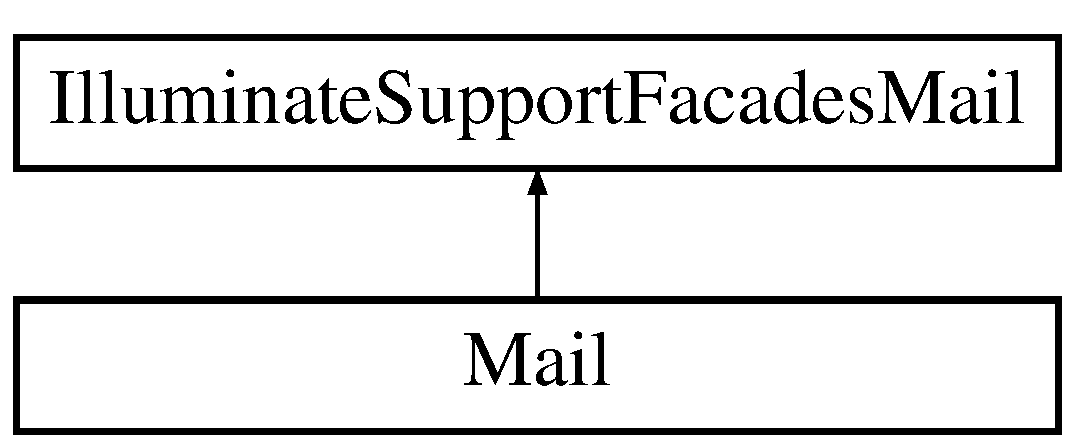
\includegraphics[height=2.000000cm]{class_mail}
\end{center}
\end{figure}
\subsection*{Additional Inherited Members}


The documentation for this class was generated from the following file\+:\begin{DoxyCompactItemize}
\item 
\+\_\+ide\+\_\+helper.\+php\end{DoxyCompactItemize}

\hypertarget{class_notification}{}\section{Notification Class Reference}
\label{class_notification}\index{Notification@{Notification}}
Inheritance diagram for Notification\+:\begin{figure}[H]
\begin{center}
\leavevmode
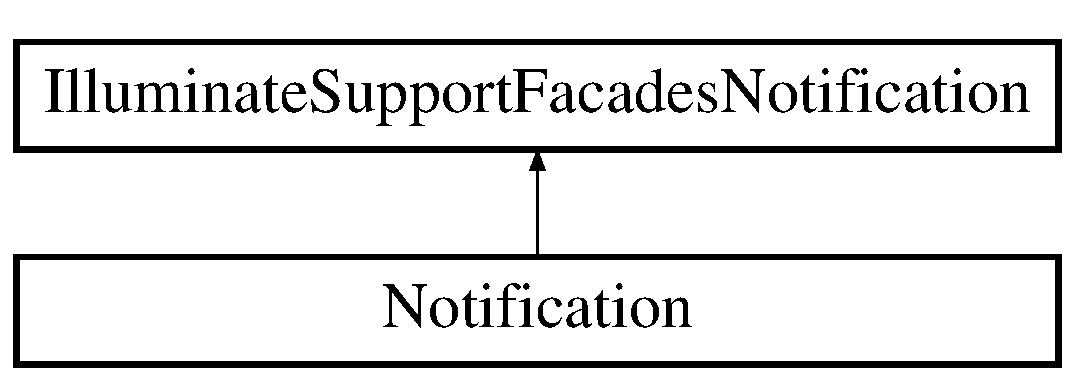
\includegraphics[height=2.000000cm]{class_notification}
\end{center}
\end{figure}
\subsection*{Additional Inherited Members}


The documentation for this class was generated from the following file\+:\begin{DoxyCompactItemize}
\item 
\+\_\+ide\+\_\+helper.\+php\end{DoxyCompactItemize}

\hypertarget{class_illuminate_1_1_support_1_1_facades_1_1_notification}{}\section{Illuminate\textbackslash{}Support\textbackslash{}Facades\textbackslash{}Notification Class Reference}
\label{class_illuminate_1_1_support_1_1_facades_1_1_notification}\index{Illuminate\textbackslash{}\+Support\textbackslash{}\+Facades\textbackslash{}\+Notification@{Illuminate\textbackslash{}\+Support\textbackslash{}\+Facades\textbackslash{}\+Notification}}
Inheritance diagram for Illuminate\textbackslash{}Support\textbackslash{}Facades\textbackslash{}Notification\+:\begin{figure}[H]
\begin{center}
\leavevmode
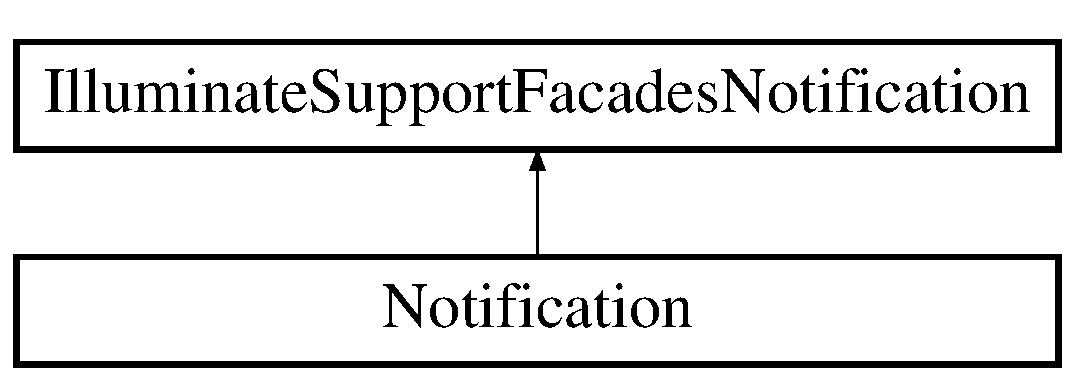
\includegraphics[height=2.000000cm]{class_illuminate_1_1_support_1_1_facades_1_1_notification}
\end{center}
\end{figure}
\subsection*{Static Public Member Functions}
\begin{DoxyCompactItemize}
\item 
static \mbox{\hyperlink{class_illuminate_1_1_support_1_1_facades_1_1_notification_a31adb0465773570a5615db01b7614e1d}{send}} (\$notifiables, \$notification)
\item 
static \mbox{\hyperlink{class_illuminate_1_1_support_1_1_facades_1_1_notification_a819fe4008c9dae1b5e73ed545c38da28}{send\+Now}} (\$notifiables, \$notification, \$channels=null)
\item 
static \mbox{\hyperlink{class_illuminate_1_1_support_1_1_facades_1_1_notification_a4b78c2b99146e23280f66bb0583b3b86}{channel}} (\$name=null)
\item 
static \mbox{\hyperlink{class_illuminate_1_1_support_1_1_facades_1_1_notification_ab82a413b9b4724ddea3c230968b7f986}{get\+Default\+Driver}} ()
\item 
static \mbox{\hyperlink{class_illuminate_1_1_support_1_1_facades_1_1_notification_ad85a8e98cfaac2699104bee89e9432ed}{delivers\+Via}} ()
\item 
static \mbox{\hyperlink{class_illuminate_1_1_support_1_1_facades_1_1_notification_ad63d78e3070748dcea4d9b54fd775312}{deliver\+Via}} (\$\mbox{\hyperlink{class_illuminate_1_1_support_1_1_facades_1_1_notification_a4b78c2b99146e23280f66bb0583b3b86}{channel}})
\item 
static \mbox{\hyperlink{class_illuminate_1_1_support_1_1_facades_1_1_notification_a47a033fe464871a4d6a6279a157effcf}{driver}} (\$driver=null)
\item 
static \mbox{\hyperlink{class_illuminate_1_1_support_1_1_facades_1_1_notification_a584448fd4e1ce7434b76b0a8dd274352}{extend}} (\$\mbox{\hyperlink{class_illuminate_1_1_support_1_1_facades_1_1_notification_a47a033fe464871a4d6a6279a157effcf}{driver}}, \$callback)
\item 
static \mbox{\hyperlink{class_illuminate_1_1_support_1_1_facades_1_1_notification_ab3df521a78ceb9f83d41e0e8af054936}{get\+Drivers}} ()
\end{DoxyCompactItemize}


\subsection{Member Function Documentation}
\mbox{\Hypertarget{class_illuminate_1_1_support_1_1_facades_1_1_notification_a4b78c2b99146e23280f66bb0583b3b86}\label{class_illuminate_1_1_support_1_1_facades_1_1_notification_a4b78c2b99146e23280f66bb0583b3b86}} 
\index{Illuminate\+::\+Support\+::\+Facades\+::\+Notification@{Illuminate\+::\+Support\+::\+Facades\+::\+Notification}!channel@{channel}}
\index{channel@{channel}!Illuminate\+::\+Support\+::\+Facades\+::\+Notification@{Illuminate\+::\+Support\+::\+Facades\+::\+Notification}}
\subsubsection{\texorpdfstring{channel()}{channel()}}
{\footnotesize\ttfamily static Illuminate\textbackslash{}\+Support\textbackslash{}\+Facades\textbackslash{}\+Notification\+::channel (\begin{DoxyParamCaption}\item[{}]{\$name = {\ttfamily null} }\end{DoxyParamCaption})\hspace{0.3cm}{\ttfamily [static]}}

Get a channel instance.


\begin{DoxyParams}[1]{Parameters}
string | null & {\em \$name} & \\
\hline
\end{DoxyParams}
\begin{DoxyReturn}{Returns}
mixed 
\end{DoxyReturn}
\mbox{\Hypertarget{class_illuminate_1_1_support_1_1_facades_1_1_notification_ad85a8e98cfaac2699104bee89e9432ed}\label{class_illuminate_1_1_support_1_1_facades_1_1_notification_ad85a8e98cfaac2699104bee89e9432ed}} 
\index{Illuminate\+::\+Support\+::\+Facades\+::\+Notification@{Illuminate\+::\+Support\+::\+Facades\+::\+Notification}!delivers\+Via@{delivers\+Via}}
\index{delivers\+Via@{delivers\+Via}!Illuminate\+::\+Support\+::\+Facades\+::\+Notification@{Illuminate\+::\+Support\+::\+Facades\+::\+Notification}}
\subsubsection{\texorpdfstring{delivers\+Via()}{deliversVia()}}
{\footnotesize\ttfamily static Illuminate\textbackslash{}\+Support\textbackslash{}\+Facades\textbackslash{}\+Notification\+::delivers\+Via (\begin{DoxyParamCaption}{ }\end{DoxyParamCaption})\hspace{0.3cm}{\ttfamily [static]}}

Get the default channel driver name.

\begin{DoxyReturn}{Returns}
string 
\end{DoxyReturn}
\mbox{\Hypertarget{class_illuminate_1_1_support_1_1_facades_1_1_notification_ad63d78e3070748dcea4d9b54fd775312}\label{class_illuminate_1_1_support_1_1_facades_1_1_notification_ad63d78e3070748dcea4d9b54fd775312}} 
\index{Illuminate\+::\+Support\+::\+Facades\+::\+Notification@{Illuminate\+::\+Support\+::\+Facades\+::\+Notification}!deliver\+Via@{deliver\+Via}}
\index{deliver\+Via@{deliver\+Via}!Illuminate\+::\+Support\+::\+Facades\+::\+Notification@{Illuminate\+::\+Support\+::\+Facades\+::\+Notification}}
\subsubsection{\texorpdfstring{deliver\+Via()}{deliverVia()}}
{\footnotesize\ttfamily static Illuminate\textbackslash{}\+Support\textbackslash{}\+Facades\textbackslash{}\+Notification\+::deliver\+Via (\begin{DoxyParamCaption}\item[{}]{\$channel }\end{DoxyParamCaption})\hspace{0.3cm}{\ttfamily [static]}}

Set the default channel driver name.


\begin{DoxyParams}[1]{Parameters}
string & {\em \$channel} & \\
\hline
\end{DoxyParams}
\begin{DoxyReturn}{Returns}
void 
\end{DoxyReturn}
\mbox{\Hypertarget{class_illuminate_1_1_support_1_1_facades_1_1_notification_a47a033fe464871a4d6a6279a157effcf}\label{class_illuminate_1_1_support_1_1_facades_1_1_notification_a47a033fe464871a4d6a6279a157effcf}} 
\index{Illuminate\+::\+Support\+::\+Facades\+::\+Notification@{Illuminate\+::\+Support\+::\+Facades\+::\+Notification}!driver@{driver}}
\index{driver@{driver}!Illuminate\+::\+Support\+::\+Facades\+::\+Notification@{Illuminate\+::\+Support\+::\+Facades\+::\+Notification}}
\subsubsection{\texorpdfstring{driver()}{driver()}}
{\footnotesize\ttfamily static Illuminate\textbackslash{}\+Support\textbackslash{}\+Facades\textbackslash{}\+Notification\+::driver (\begin{DoxyParamCaption}\item[{}]{\$driver = {\ttfamily null} }\end{DoxyParamCaption})\hspace{0.3cm}{\ttfamily [static]}}

Get a driver instance.


\begin{DoxyParams}[1]{Parameters}
string & {\em \$driver} & \\
\hline
\end{DoxyParams}
\begin{DoxyReturn}{Returns}
mixed 
\end{DoxyReturn}
\mbox{\Hypertarget{class_illuminate_1_1_support_1_1_facades_1_1_notification_a584448fd4e1ce7434b76b0a8dd274352}\label{class_illuminate_1_1_support_1_1_facades_1_1_notification_a584448fd4e1ce7434b76b0a8dd274352}} 
\index{Illuminate\+::\+Support\+::\+Facades\+::\+Notification@{Illuminate\+::\+Support\+::\+Facades\+::\+Notification}!extend@{extend}}
\index{extend@{extend}!Illuminate\+::\+Support\+::\+Facades\+::\+Notification@{Illuminate\+::\+Support\+::\+Facades\+::\+Notification}}
\subsubsection{\texorpdfstring{extend()}{extend()}}
{\footnotesize\ttfamily static Illuminate\textbackslash{}\+Support\textbackslash{}\+Facades\textbackslash{}\+Notification\+::extend (\begin{DoxyParamCaption}\item[{}]{\$driver,  }\item[{}]{\$callback }\end{DoxyParamCaption})\hspace{0.3cm}{\ttfamily [static]}}

Register a custom driver creator Closure.


\begin{DoxyParams}[1]{Parameters}
string & {\em \$driver} & \\
\hline
\textbackslash{}\+Closure & {\em \$callback} & \\
\hline
\end{DoxyParams}
\begin{DoxyReturn}{Returns}
\$this 
\end{DoxyReturn}
\mbox{\Hypertarget{class_illuminate_1_1_support_1_1_facades_1_1_notification_ab82a413b9b4724ddea3c230968b7f986}\label{class_illuminate_1_1_support_1_1_facades_1_1_notification_ab82a413b9b4724ddea3c230968b7f986}} 
\index{Illuminate\+::\+Support\+::\+Facades\+::\+Notification@{Illuminate\+::\+Support\+::\+Facades\+::\+Notification}!get\+Default\+Driver@{get\+Default\+Driver}}
\index{get\+Default\+Driver@{get\+Default\+Driver}!Illuminate\+::\+Support\+::\+Facades\+::\+Notification@{Illuminate\+::\+Support\+::\+Facades\+::\+Notification}}
\subsubsection{\texorpdfstring{get\+Default\+Driver()}{getDefaultDriver()}}
{\footnotesize\ttfamily static Illuminate\textbackslash{}\+Support\textbackslash{}\+Facades\textbackslash{}\+Notification\+::get\+Default\+Driver (\begin{DoxyParamCaption}{ }\end{DoxyParamCaption})\hspace{0.3cm}{\ttfamily [static]}}

Get the default channel driver name.

\begin{DoxyReturn}{Returns}
string 
\end{DoxyReturn}
\mbox{\Hypertarget{class_illuminate_1_1_support_1_1_facades_1_1_notification_ab3df521a78ceb9f83d41e0e8af054936}\label{class_illuminate_1_1_support_1_1_facades_1_1_notification_ab3df521a78ceb9f83d41e0e8af054936}} 
\index{Illuminate\+::\+Support\+::\+Facades\+::\+Notification@{Illuminate\+::\+Support\+::\+Facades\+::\+Notification}!get\+Drivers@{get\+Drivers}}
\index{get\+Drivers@{get\+Drivers}!Illuminate\+::\+Support\+::\+Facades\+::\+Notification@{Illuminate\+::\+Support\+::\+Facades\+::\+Notification}}
\subsubsection{\texorpdfstring{get\+Drivers()}{getDrivers()}}
{\footnotesize\ttfamily static Illuminate\textbackslash{}\+Support\textbackslash{}\+Facades\textbackslash{}\+Notification\+::get\+Drivers (\begin{DoxyParamCaption}{ }\end{DoxyParamCaption})\hspace{0.3cm}{\ttfamily [static]}}

Get all of the created \char`\"{}drivers\char`\"{}.

\begin{DoxyReturn}{Returns}
array 
\end{DoxyReturn}
\mbox{\Hypertarget{class_illuminate_1_1_support_1_1_facades_1_1_notification_a31adb0465773570a5615db01b7614e1d}\label{class_illuminate_1_1_support_1_1_facades_1_1_notification_a31adb0465773570a5615db01b7614e1d}} 
\index{Illuminate\+::\+Support\+::\+Facades\+::\+Notification@{Illuminate\+::\+Support\+::\+Facades\+::\+Notification}!send@{send}}
\index{send@{send}!Illuminate\+::\+Support\+::\+Facades\+::\+Notification@{Illuminate\+::\+Support\+::\+Facades\+::\+Notification}}
\subsubsection{\texorpdfstring{send()}{send()}}
{\footnotesize\ttfamily static Illuminate\textbackslash{}\+Support\textbackslash{}\+Facades\textbackslash{}\+Notification\+::send (\begin{DoxyParamCaption}\item[{}]{\$notifiables,  }\item[{}]{\$notification }\end{DoxyParamCaption})\hspace{0.3cm}{\ttfamily [static]}}

Send the given notification to the given notifiable entities.


\begin{DoxyParams}[1]{Parameters}
\textbackslash{}\+Illuminate\textbackslash{}\+Support\textbackslash{}\+Collection | array | mixed & {\em \$notifiables} & \\
\hline
mixed & {\em \$notification} & \\
\hline
\end{DoxyParams}
\begin{DoxyReturn}{Returns}
void 
\end{DoxyReturn}
\mbox{\Hypertarget{class_illuminate_1_1_support_1_1_facades_1_1_notification_a819fe4008c9dae1b5e73ed545c38da28}\label{class_illuminate_1_1_support_1_1_facades_1_1_notification_a819fe4008c9dae1b5e73ed545c38da28}} 
\index{Illuminate\+::\+Support\+::\+Facades\+::\+Notification@{Illuminate\+::\+Support\+::\+Facades\+::\+Notification}!send\+Now@{send\+Now}}
\index{send\+Now@{send\+Now}!Illuminate\+::\+Support\+::\+Facades\+::\+Notification@{Illuminate\+::\+Support\+::\+Facades\+::\+Notification}}
\subsubsection{\texorpdfstring{send\+Now()}{sendNow()}}
{\footnotesize\ttfamily static Illuminate\textbackslash{}\+Support\textbackslash{}\+Facades\textbackslash{}\+Notification\+::send\+Now (\begin{DoxyParamCaption}\item[{}]{\$notifiables,  }\item[{}]{\$notification,  }\item[{}]{\$channels = {\ttfamily null} }\end{DoxyParamCaption})\hspace{0.3cm}{\ttfamily [static]}}

Send the given notification immediately.


\begin{DoxyParams}[1]{Parameters}
\textbackslash{}\+Illuminate\textbackslash{}\+Support\textbackslash{}\+Collection | array | mixed & {\em \$notifiables} & \\
\hline
mixed & {\em \$notification} & \\
\hline
array | null & {\em \$channels} & \\
\hline
\end{DoxyParams}
\begin{DoxyReturn}{Returns}
void 
\end{DoxyReturn}


The documentation for this class was generated from the following file\+:\begin{DoxyCompactItemize}
\item 
\+\_\+ide\+\_\+helper.\+php\end{DoxyCompactItemize}

\hypertarget{class_illuminate_1_1_support_1_1_facades_1_1_password}{}\section{Illuminate\textbackslash{}Support\textbackslash{}Facades\textbackslash{}Password Class Reference}
\label{class_illuminate_1_1_support_1_1_facades_1_1_password}\index{Illuminate\textbackslash{}\+Support\textbackslash{}\+Facades\textbackslash{}\+Password@{Illuminate\textbackslash{}\+Support\textbackslash{}\+Facades\textbackslash{}\+Password}}
Inheritance diagram for Illuminate\textbackslash{}Support\textbackslash{}Facades\textbackslash{}Password\+:\begin{figure}[H]
\begin{center}
\leavevmode
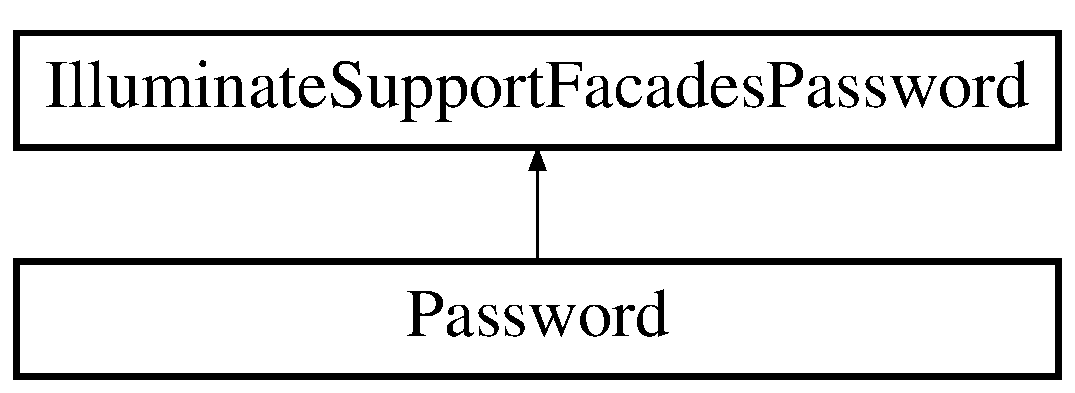
\includegraphics[height=2.000000cm]{class_illuminate_1_1_support_1_1_facades_1_1_password}
\end{center}
\end{figure}
\subsection*{Static Public Member Functions}
\begin{DoxyCompactItemize}
\item 
static \mbox{\hyperlink{class_illuminate_1_1_support_1_1_facades_1_1_password_a2ab3d512f33afab7e4a6d30451b73004}{broker}} (\$name=null)
\item 
static \mbox{\hyperlink{class_illuminate_1_1_support_1_1_facades_1_1_password_af71d4c568356b6fc983c3afc99687a10}{get\+Default\+Driver}} ()
\item 
static \mbox{\hyperlink{class_illuminate_1_1_support_1_1_facades_1_1_password_ae2ba5566739028f4836fed084f77daa1}{set\+Default\+Driver}} (\$name)
\end{DoxyCompactItemize}


\subsection{Member Function Documentation}
\mbox{\Hypertarget{class_illuminate_1_1_support_1_1_facades_1_1_password_a2ab3d512f33afab7e4a6d30451b73004}\label{class_illuminate_1_1_support_1_1_facades_1_1_password_a2ab3d512f33afab7e4a6d30451b73004}} 
\index{Illuminate\+::\+Support\+::\+Facades\+::\+Password@{Illuminate\+::\+Support\+::\+Facades\+::\+Password}!broker@{broker}}
\index{broker@{broker}!Illuminate\+::\+Support\+::\+Facades\+::\+Password@{Illuminate\+::\+Support\+::\+Facades\+::\+Password}}
\subsubsection{\texorpdfstring{broker()}{broker()}}
{\footnotesize\ttfamily static Illuminate\textbackslash{}\+Support\textbackslash{}\+Facades\textbackslash{}\+Password\+::broker (\begin{DoxyParamCaption}\item[{}]{\$name = {\ttfamily null} }\end{DoxyParamCaption})\hspace{0.3cm}{\ttfamily [static]}}

Attempt to get the broker from the local cache.


\begin{DoxyParams}[1]{Parameters}
string & {\em \$name} & \\
\hline
\end{DoxyParams}
\begin{DoxyReturn}{Returns}

\end{DoxyReturn}
\mbox{\Hypertarget{class_illuminate_1_1_support_1_1_facades_1_1_password_af71d4c568356b6fc983c3afc99687a10}\label{class_illuminate_1_1_support_1_1_facades_1_1_password_af71d4c568356b6fc983c3afc99687a10}} 
\index{Illuminate\+::\+Support\+::\+Facades\+::\+Password@{Illuminate\+::\+Support\+::\+Facades\+::\+Password}!get\+Default\+Driver@{get\+Default\+Driver}}
\index{get\+Default\+Driver@{get\+Default\+Driver}!Illuminate\+::\+Support\+::\+Facades\+::\+Password@{Illuminate\+::\+Support\+::\+Facades\+::\+Password}}
\subsubsection{\texorpdfstring{get\+Default\+Driver()}{getDefaultDriver()}}
{\footnotesize\ttfamily static Illuminate\textbackslash{}\+Support\textbackslash{}\+Facades\textbackslash{}\+Password\+::get\+Default\+Driver (\begin{DoxyParamCaption}{ }\end{DoxyParamCaption})\hspace{0.3cm}{\ttfamily [static]}}

Get the default password broker name.

\begin{DoxyReturn}{Returns}
string 
\end{DoxyReturn}
\mbox{\Hypertarget{class_illuminate_1_1_support_1_1_facades_1_1_password_ae2ba5566739028f4836fed084f77daa1}\label{class_illuminate_1_1_support_1_1_facades_1_1_password_ae2ba5566739028f4836fed084f77daa1}} 
\index{Illuminate\+::\+Support\+::\+Facades\+::\+Password@{Illuminate\+::\+Support\+::\+Facades\+::\+Password}!set\+Default\+Driver@{set\+Default\+Driver}}
\index{set\+Default\+Driver@{set\+Default\+Driver}!Illuminate\+::\+Support\+::\+Facades\+::\+Password@{Illuminate\+::\+Support\+::\+Facades\+::\+Password}}
\subsubsection{\texorpdfstring{set\+Default\+Driver()}{setDefaultDriver()}}
{\footnotesize\ttfamily static Illuminate\textbackslash{}\+Support\textbackslash{}\+Facades\textbackslash{}\+Password\+::set\+Default\+Driver (\begin{DoxyParamCaption}\item[{}]{\$name }\end{DoxyParamCaption})\hspace{0.3cm}{\ttfamily [static]}}

Set the default password broker name.


\begin{DoxyParams}[1]{Parameters}
string & {\em \$name} & \\
\hline
\end{DoxyParams}
\begin{DoxyReturn}{Returns}
void 
\end{DoxyReturn}


The documentation for this class was generated from the following file\+:\begin{DoxyCompactItemize}
\item 
\+\_\+ide\+\_\+helper.\+php\end{DoxyCompactItemize}

\hypertarget{class_password}{}\section{Password Class Reference}
\label{class_password}\index{Password@{Password}}
Inheritance diagram for Password\+:\begin{figure}[H]
\begin{center}
\leavevmode
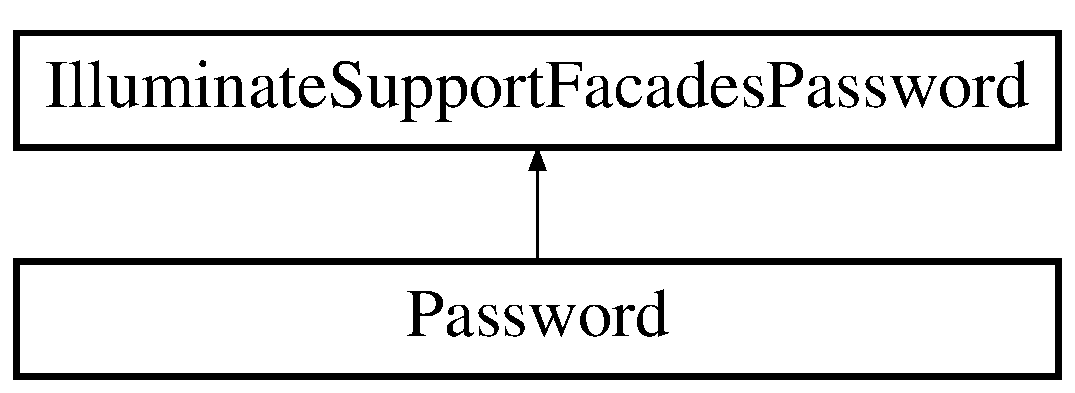
\includegraphics[height=2.000000cm]{class_password}
\end{center}
\end{figure}
\subsection*{Additional Inherited Members}


The documentation for this class was generated from the following file\+:\begin{DoxyCompactItemize}
\item 
\+\_\+ide\+\_\+helper.\+php\end{DoxyCompactItemize}

\hypertarget{class_queue}{}\section{Queue Class Reference}
\label{class_queue}\index{Queue@{Queue}}
Inheritance diagram for Queue\+:\begin{figure}[H]
\begin{center}
\leavevmode
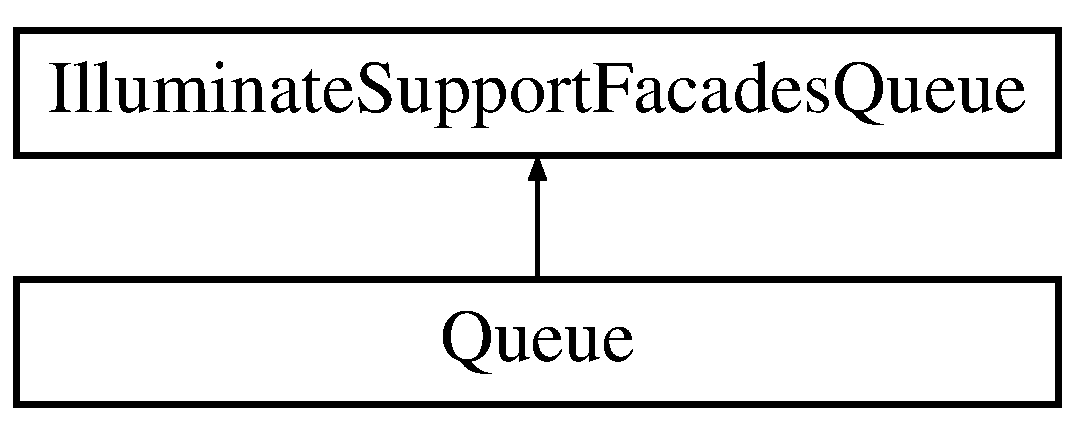
\includegraphics[height=2.000000cm]{class_queue}
\end{center}
\end{figure}
\subsection*{Additional Inherited Members}


The documentation for this class was generated from the following file\+:\begin{DoxyCompactItemize}
\item 
\+\_\+ide\+\_\+helper.\+php\end{DoxyCompactItemize}

\hypertarget{class_illuminate_1_1_support_1_1_facades_1_1_queue}{}\section{Illuminate\textbackslash{}Support\textbackslash{}Facades\textbackslash{}Queue Class Reference}
\label{class_illuminate_1_1_support_1_1_facades_1_1_queue}\index{Illuminate\textbackslash{}\+Support\textbackslash{}\+Facades\textbackslash{}\+Queue@{Illuminate\textbackslash{}\+Support\textbackslash{}\+Facades\textbackslash{}\+Queue}}
Inheritance diagram for Illuminate\textbackslash{}Support\textbackslash{}Facades\textbackslash{}Queue\+:\begin{figure}[H]
\begin{center}
\leavevmode
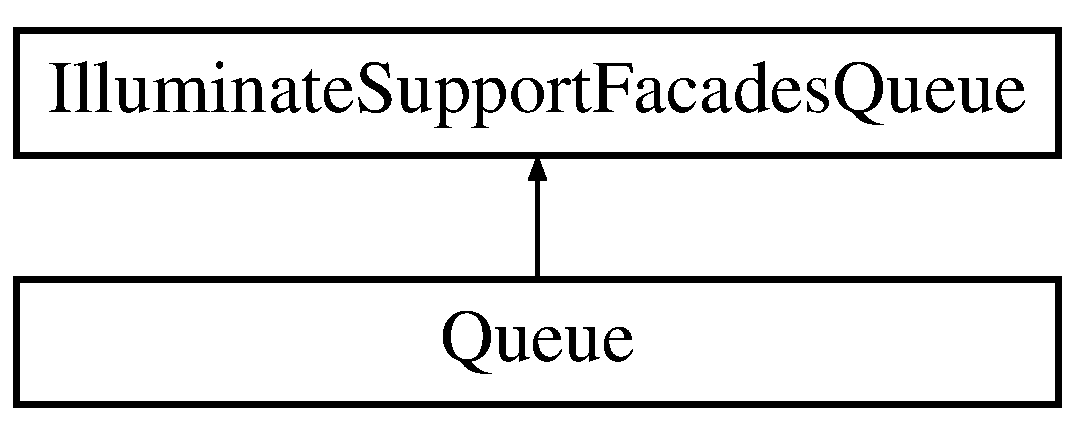
\includegraphics[height=2.000000cm]{class_illuminate_1_1_support_1_1_facades_1_1_queue}
\end{center}
\end{figure}
\subsection*{Static Public Member Functions}
\begin{DoxyCompactItemize}
\item 
static \mbox{\hyperlink{class_illuminate_1_1_support_1_1_facades_1_1_queue_a98b4d092f13b6ad01c075f2790c15b40}{before}} (\$callback)
\item 
static \mbox{\hyperlink{class_illuminate_1_1_support_1_1_facades_1_1_queue_ab9c41644bd797b45622ab16eb93154f6}{after}} (\$callback)
\item 
static \mbox{\hyperlink{class_illuminate_1_1_support_1_1_facades_1_1_queue_aa9660b4de41a9ebb4f7dd26c8071a6da}{exception\+Occurred}} (\$callback)
\item 
static \mbox{\hyperlink{class_illuminate_1_1_support_1_1_facades_1_1_queue_a30bd51b47c8eea09ab5b11261c45efef}{looping}} (\$callback)
\item 
static \mbox{\hyperlink{class_illuminate_1_1_support_1_1_facades_1_1_queue_ad643d2fc351875a68b8327d3717eb514}{failing}} (\$callback)
\item 
static \mbox{\hyperlink{class_illuminate_1_1_support_1_1_facades_1_1_queue_af1dce728ca2ce292a6034d11bbd067a9}{stopping}} (\$callback)
\item 
static \mbox{\hyperlink{class_illuminate_1_1_support_1_1_facades_1_1_queue_a8f3205c731d192e78c749b4a586f9c48}{connected}} (\$name=null)
\item 
static \mbox{\hyperlink{class_illuminate_1_1_support_1_1_facades_1_1_queue_ac72dcbbe7e5f6b8366c31c30881af7fe}{connection}} (\$name=null)
\item 
static \mbox{\hyperlink{class_illuminate_1_1_support_1_1_facades_1_1_queue_ad95bc43c71e4d5191be6bfa129fe4170}{extend}} (\$driver, \$resolver)
\item 
static \mbox{\hyperlink{class_illuminate_1_1_support_1_1_facades_1_1_queue_a042f522a7874b4464d8756bf4d351501}{add\+Connector}} (\$driver, \$resolver)
\item 
static \mbox{\hyperlink{class_illuminate_1_1_support_1_1_facades_1_1_queue_a8146531a36a958787fac1ea14f54bdd3}{get\+Default\+Driver}} ()
\item 
static \mbox{\hyperlink{class_illuminate_1_1_support_1_1_facades_1_1_queue_a09145f9150bdb92fd6dbcc95511089b5}{set\+Default\+Driver}} (\$name)
\item 
static \mbox{\hyperlink{class_illuminate_1_1_support_1_1_facades_1_1_queue_a86e8629ef502a46f0a4c9255e740b550}{get\+Name}} (\$\mbox{\hyperlink{class_illuminate_1_1_support_1_1_facades_1_1_queue_ac72dcbbe7e5f6b8366c31c30881af7fe}{connection}}=null)
\item 
static \mbox{\hyperlink{class_illuminate_1_1_support_1_1_facades_1_1_queue_a07ac76a4da451f5a76cfe17ea32bccd0}{is\+Down\+For\+Maintenance}} ()
\item 
static \mbox{\hyperlink{class_illuminate_1_1_support_1_1_facades_1_1_queue_a0a67d96dfa53c28ed1f46e5bc9b99133}{size}} (\$queue=null)
\item 
static \mbox{\hyperlink{class_illuminate_1_1_support_1_1_facades_1_1_queue_a089d965181938d50eb14b2b02b13000d}{push}} (\$job, \$data=\textquotesingle{}\textquotesingle{}, \$queue=null)
\item 
static \mbox{\hyperlink{class_illuminate_1_1_support_1_1_facades_1_1_queue_aad2749d558a9aa33ca546fe14698fc0b}{push\+Raw}} (\$payload, \$queue=null, \$options=array())
\item 
static \mbox{\hyperlink{class_illuminate_1_1_support_1_1_facades_1_1_queue_a0c240253396403c946d0ea7d10f6bb87}{later}} (\$delay, \$job, \$data=\textquotesingle{}\textquotesingle{}, \$queue=null)
\item 
static \mbox{\hyperlink{class_illuminate_1_1_support_1_1_facades_1_1_queue_a141667b7e321120b3ca7ac7968ec3bf5}{pop}} (\$queue=null)
\item 
static \mbox{\hyperlink{class_illuminate_1_1_support_1_1_facades_1_1_queue_a3a93abf7cc4bb41b49d78ef0927967f7}{push\+On}} (\$queue, \$job, \$data=\textquotesingle{}\textquotesingle{})
\item 
static \mbox{\hyperlink{class_illuminate_1_1_support_1_1_facades_1_1_queue_a27a4e841c8af2c85e28b199ecc7da3ef}{later\+On}} (\$queue, \$delay, \$job, \$data=\textquotesingle{}\textquotesingle{})
\item 
static \mbox{\hyperlink{class_illuminate_1_1_support_1_1_facades_1_1_queue_a49cac55a7c41728b0c1a7e42397384c9}{bulk}} (\$jobs, \$data=\textquotesingle{}\textquotesingle{}, \$queue=null)
\item 
static \mbox{\hyperlink{class_illuminate_1_1_support_1_1_facades_1_1_queue_a8f37124b980065ea0afb7914dd7467d5}{get\+Job\+Expiration}} (\$job)
\item 
static \mbox{\hyperlink{class_illuminate_1_1_support_1_1_facades_1_1_queue_a1951ce66a067f286771d81530fbf200a}{get\+Connection\+Name}} ()
\item 
static \mbox{\hyperlink{class_illuminate_1_1_support_1_1_facades_1_1_queue_a9dd6771189e2ad44140e77c702f265dc}{set\+Connection\+Name}} (\$name)
\item 
static \mbox{\hyperlink{class_illuminate_1_1_support_1_1_facades_1_1_queue_a63c45aa8d429ab7713cf1bcf52d4fc77}{set\+Container}} (\$container)
\end{DoxyCompactItemize}


\subsection{Member Function Documentation}
\mbox{\Hypertarget{class_illuminate_1_1_support_1_1_facades_1_1_queue_a042f522a7874b4464d8756bf4d351501}\label{class_illuminate_1_1_support_1_1_facades_1_1_queue_a042f522a7874b4464d8756bf4d351501}} 
\index{Illuminate\+::\+Support\+::\+Facades\+::\+Queue@{Illuminate\+::\+Support\+::\+Facades\+::\+Queue}!add\+Connector@{add\+Connector}}
\index{add\+Connector@{add\+Connector}!Illuminate\+::\+Support\+::\+Facades\+::\+Queue@{Illuminate\+::\+Support\+::\+Facades\+::\+Queue}}
\subsubsection{\texorpdfstring{add\+Connector()}{addConnector()}}
{\footnotesize\ttfamily static Illuminate\textbackslash{}\+Support\textbackslash{}\+Facades\textbackslash{}\+Queue\+::add\+Connector (\begin{DoxyParamCaption}\item[{}]{\$driver,  }\item[{}]{\$resolver }\end{DoxyParamCaption})\hspace{0.3cm}{\ttfamily [static]}}

Add a queue connection resolver.


\begin{DoxyParams}[1]{Parameters}
string & {\em \$driver} & \\
\hline
\textbackslash{}\+Closure & {\em \$resolver} & \\
\hline
\end{DoxyParams}
\begin{DoxyReturn}{Returns}
void 
\end{DoxyReturn}
\mbox{\Hypertarget{class_illuminate_1_1_support_1_1_facades_1_1_queue_ab9c41644bd797b45622ab16eb93154f6}\label{class_illuminate_1_1_support_1_1_facades_1_1_queue_ab9c41644bd797b45622ab16eb93154f6}} 
\index{Illuminate\+::\+Support\+::\+Facades\+::\+Queue@{Illuminate\+::\+Support\+::\+Facades\+::\+Queue}!after@{after}}
\index{after@{after}!Illuminate\+::\+Support\+::\+Facades\+::\+Queue@{Illuminate\+::\+Support\+::\+Facades\+::\+Queue}}
\subsubsection{\texorpdfstring{after()}{after()}}
{\footnotesize\ttfamily static Illuminate\textbackslash{}\+Support\textbackslash{}\+Facades\textbackslash{}\+Queue\+::after (\begin{DoxyParamCaption}\item[{}]{\$callback }\end{DoxyParamCaption})\hspace{0.3cm}{\ttfamily [static]}}

Register an event listener for the after job event.


\begin{DoxyParams}[1]{Parameters}
mixed & {\em \$callback} & \\
\hline
\end{DoxyParams}
\begin{DoxyReturn}{Returns}
void 
\end{DoxyReturn}
\mbox{\Hypertarget{class_illuminate_1_1_support_1_1_facades_1_1_queue_a98b4d092f13b6ad01c075f2790c15b40}\label{class_illuminate_1_1_support_1_1_facades_1_1_queue_a98b4d092f13b6ad01c075f2790c15b40}} 
\index{Illuminate\+::\+Support\+::\+Facades\+::\+Queue@{Illuminate\+::\+Support\+::\+Facades\+::\+Queue}!before@{before}}
\index{before@{before}!Illuminate\+::\+Support\+::\+Facades\+::\+Queue@{Illuminate\+::\+Support\+::\+Facades\+::\+Queue}}
\subsubsection{\texorpdfstring{before()}{before()}}
{\footnotesize\ttfamily static Illuminate\textbackslash{}\+Support\textbackslash{}\+Facades\textbackslash{}\+Queue\+::before (\begin{DoxyParamCaption}\item[{}]{\$callback }\end{DoxyParamCaption})\hspace{0.3cm}{\ttfamily [static]}}

Register an event listener for the before job event.


\begin{DoxyParams}[1]{Parameters}
mixed & {\em \$callback} & \\
\hline
\end{DoxyParams}
\begin{DoxyReturn}{Returns}
void 
\end{DoxyReturn}
\mbox{\Hypertarget{class_illuminate_1_1_support_1_1_facades_1_1_queue_a49cac55a7c41728b0c1a7e42397384c9}\label{class_illuminate_1_1_support_1_1_facades_1_1_queue_a49cac55a7c41728b0c1a7e42397384c9}} 
\index{Illuminate\+::\+Support\+::\+Facades\+::\+Queue@{Illuminate\+::\+Support\+::\+Facades\+::\+Queue}!bulk@{bulk}}
\index{bulk@{bulk}!Illuminate\+::\+Support\+::\+Facades\+::\+Queue@{Illuminate\+::\+Support\+::\+Facades\+::\+Queue}}
\subsubsection{\texorpdfstring{bulk()}{bulk()}}
{\footnotesize\ttfamily static Illuminate\textbackslash{}\+Support\textbackslash{}\+Facades\textbackslash{}\+Queue\+::bulk (\begin{DoxyParamCaption}\item[{}]{\$jobs,  }\item[{}]{\$data = {\ttfamily \textquotesingle{}\textquotesingle{}},  }\item[{}]{\$queue = {\ttfamily null} }\end{DoxyParamCaption})\hspace{0.3cm}{\ttfamily [static]}}

Push an array of jobs onto the queue.


\begin{DoxyParams}[1]{Parameters}
array & {\em \$jobs} & \\
\hline
mixed & {\em \$data} & \\
\hline
string & {\em \$queue} & \\
\hline
\end{DoxyParams}
\begin{DoxyReturn}{Returns}
mixed 
\end{DoxyReturn}
\mbox{\Hypertarget{class_illuminate_1_1_support_1_1_facades_1_1_queue_a8f3205c731d192e78c749b4a586f9c48}\label{class_illuminate_1_1_support_1_1_facades_1_1_queue_a8f3205c731d192e78c749b4a586f9c48}} 
\index{Illuminate\+::\+Support\+::\+Facades\+::\+Queue@{Illuminate\+::\+Support\+::\+Facades\+::\+Queue}!connected@{connected}}
\index{connected@{connected}!Illuminate\+::\+Support\+::\+Facades\+::\+Queue@{Illuminate\+::\+Support\+::\+Facades\+::\+Queue}}
\subsubsection{\texorpdfstring{connected()}{connected()}}
{\footnotesize\ttfamily static Illuminate\textbackslash{}\+Support\textbackslash{}\+Facades\textbackslash{}\+Queue\+::connected (\begin{DoxyParamCaption}\item[{}]{\$name = {\ttfamily null} }\end{DoxyParamCaption})\hspace{0.3cm}{\ttfamily [static]}}

Determine if the driver is connected.


\begin{DoxyParams}[1]{Parameters}
string & {\em \$name} & \\
\hline
\end{DoxyParams}
\begin{DoxyReturn}{Returns}
bool 
\end{DoxyReturn}
\mbox{\Hypertarget{class_illuminate_1_1_support_1_1_facades_1_1_queue_ac72dcbbe7e5f6b8366c31c30881af7fe}\label{class_illuminate_1_1_support_1_1_facades_1_1_queue_ac72dcbbe7e5f6b8366c31c30881af7fe}} 
\index{Illuminate\+::\+Support\+::\+Facades\+::\+Queue@{Illuminate\+::\+Support\+::\+Facades\+::\+Queue}!connection@{connection}}
\index{connection@{connection}!Illuminate\+::\+Support\+::\+Facades\+::\+Queue@{Illuminate\+::\+Support\+::\+Facades\+::\+Queue}}
\subsubsection{\texorpdfstring{connection()}{connection()}}
{\footnotesize\ttfamily static Illuminate\textbackslash{}\+Support\textbackslash{}\+Facades\textbackslash{}\+Queue\+::connection (\begin{DoxyParamCaption}\item[{}]{\$name = {\ttfamily null} }\end{DoxyParamCaption})\hspace{0.3cm}{\ttfamily [static]}}

Resolve a queue connection instance.


\begin{DoxyParams}[1]{Parameters}
string & {\em \$name} & \\
\hline
\end{DoxyParams}
\begin{DoxyReturn}{Returns}

\end{DoxyReturn}
\mbox{\Hypertarget{class_illuminate_1_1_support_1_1_facades_1_1_queue_aa9660b4de41a9ebb4f7dd26c8071a6da}\label{class_illuminate_1_1_support_1_1_facades_1_1_queue_aa9660b4de41a9ebb4f7dd26c8071a6da}} 
\index{Illuminate\+::\+Support\+::\+Facades\+::\+Queue@{Illuminate\+::\+Support\+::\+Facades\+::\+Queue}!exception\+Occurred@{exception\+Occurred}}
\index{exception\+Occurred@{exception\+Occurred}!Illuminate\+::\+Support\+::\+Facades\+::\+Queue@{Illuminate\+::\+Support\+::\+Facades\+::\+Queue}}
\subsubsection{\texorpdfstring{exception\+Occurred()}{exceptionOccurred()}}
{\footnotesize\ttfamily static Illuminate\textbackslash{}\+Support\textbackslash{}\+Facades\textbackslash{}\+Queue\+::exception\+Occurred (\begin{DoxyParamCaption}\item[{}]{\$callback }\end{DoxyParamCaption})\hspace{0.3cm}{\ttfamily [static]}}

Register an event listener for the exception occurred job event.


\begin{DoxyParams}[1]{Parameters}
mixed & {\em \$callback} & \\
\hline
\end{DoxyParams}
\begin{DoxyReturn}{Returns}
void 
\end{DoxyReturn}
\mbox{\Hypertarget{class_illuminate_1_1_support_1_1_facades_1_1_queue_ad95bc43c71e4d5191be6bfa129fe4170}\label{class_illuminate_1_1_support_1_1_facades_1_1_queue_ad95bc43c71e4d5191be6bfa129fe4170}} 
\index{Illuminate\+::\+Support\+::\+Facades\+::\+Queue@{Illuminate\+::\+Support\+::\+Facades\+::\+Queue}!extend@{extend}}
\index{extend@{extend}!Illuminate\+::\+Support\+::\+Facades\+::\+Queue@{Illuminate\+::\+Support\+::\+Facades\+::\+Queue}}
\subsubsection{\texorpdfstring{extend()}{extend()}}
{\footnotesize\ttfamily static Illuminate\textbackslash{}\+Support\textbackslash{}\+Facades\textbackslash{}\+Queue\+::extend (\begin{DoxyParamCaption}\item[{}]{\$driver,  }\item[{}]{\$resolver }\end{DoxyParamCaption})\hspace{0.3cm}{\ttfamily [static]}}

Add a queue connection resolver.


\begin{DoxyParams}[1]{Parameters}
string & {\em \$driver} & \\
\hline
\textbackslash{}\+Closure & {\em \$resolver} & \\
\hline
\end{DoxyParams}
\begin{DoxyReturn}{Returns}
void 
\end{DoxyReturn}
\mbox{\Hypertarget{class_illuminate_1_1_support_1_1_facades_1_1_queue_ad643d2fc351875a68b8327d3717eb514}\label{class_illuminate_1_1_support_1_1_facades_1_1_queue_ad643d2fc351875a68b8327d3717eb514}} 
\index{Illuminate\+::\+Support\+::\+Facades\+::\+Queue@{Illuminate\+::\+Support\+::\+Facades\+::\+Queue}!failing@{failing}}
\index{failing@{failing}!Illuminate\+::\+Support\+::\+Facades\+::\+Queue@{Illuminate\+::\+Support\+::\+Facades\+::\+Queue}}
\subsubsection{\texorpdfstring{failing()}{failing()}}
{\footnotesize\ttfamily static Illuminate\textbackslash{}\+Support\textbackslash{}\+Facades\textbackslash{}\+Queue\+::failing (\begin{DoxyParamCaption}\item[{}]{\$callback }\end{DoxyParamCaption})\hspace{0.3cm}{\ttfamily [static]}}

Register an event listener for the failed job event.


\begin{DoxyParams}[1]{Parameters}
mixed & {\em \$callback} & \\
\hline
\end{DoxyParams}
\begin{DoxyReturn}{Returns}
void 
\end{DoxyReturn}
\mbox{\Hypertarget{class_illuminate_1_1_support_1_1_facades_1_1_queue_a1951ce66a067f286771d81530fbf200a}\label{class_illuminate_1_1_support_1_1_facades_1_1_queue_a1951ce66a067f286771d81530fbf200a}} 
\index{Illuminate\+::\+Support\+::\+Facades\+::\+Queue@{Illuminate\+::\+Support\+::\+Facades\+::\+Queue}!get\+Connection\+Name@{get\+Connection\+Name}}
\index{get\+Connection\+Name@{get\+Connection\+Name}!Illuminate\+::\+Support\+::\+Facades\+::\+Queue@{Illuminate\+::\+Support\+::\+Facades\+::\+Queue}}
\subsubsection{\texorpdfstring{get\+Connection\+Name()}{getConnectionName()}}
{\footnotesize\ttfamily static Illuminate\textbackslash{}\+Support\textbackslash{}\+Facades\textbackslash{}\+Queue\+::get\+Connection\+Name (\begin{DoxyParamCaption}{ }\end{DoxyParamCaption})\hspace{0.3cm}{\ttfamily [static]}}

Get the connection name for the queue.

\begin{DoxyReturn}{Returns}
string 
\end{DoxyReturn}
\mbox{\Hypertarget{class_illuminate_1_1_support_1_1_facades_1_1_queue_a8146531a36a958787fac1ea14f54bdd3}\label{class_illuminate_1_1_support_1_1_facades_1_1_queue_a8146531a36a958787fac1ea14f54bdd3}} 
\index{Illuminate\+::\+Support\+::\+Facades\+::\+Queue@{Illuminate\+::\+Support\+::\+Facades\+::\+Queue}!get\+Default\+Driver@{get\+Default\+Driver}}
\index{get\+Default\+Driver@{get\+Default\+Driver}!Illuminate\+::\+Support\+::\+Facades\+::\+Queue@{Illuminate\+::\+Support\+::\+Facades\+::\+Queue}}
\subsubsection{\texorpdfstring{get\+Default\+Driver()}{getDefaultDriver()}}
{\footnotesize\ttfamily static Illuminate\textbackslash{}\+Support\textbackslash{}\+Facades\textbackslash{}\+Queue\+::get\+Default\+Driver (\begin{DoxyParamCaption}{ }\end{DoxyParamCaption})\hspace{0.3cm}{\ttfamily [static]}}

Get the name of the default queue connection.

\begin{DoxyReturn}{Returns}
string 
\end{DoxyReturn}
\mbox{\Hypertarget{class_illuminate_1_1_support_1_1_facades_1_1_queue_a8f37124b980065ea0afb7914dd7467d5}\label{class_illuminate_1_1_support_1_1_facades_1_1_queue_a8f37124b980065ea0afb7914dd7467d5}} 
\index{Illuminate\+::\+Support\+::\+Facades\+::\+Queue@{Illuminate\+::\+Support\+::\+Facades\+::\+Queue}!get\+Job\+Expiration@{get\+Job\+Expiration}}
\index{get\+Job\+Expiration@{get\+Job\+Expiration}!Illuminate\+::\+Support\+::\+Facades\+::\+Queue@{Illuminate\+::\+Support\+::\+Facades\+::\+Queue}}
\subsubsection{\texorpdfstring{get\+Job\+Expiration()}{getJobExpiration()}}
{\footnotesize\ttfamily static Illuminate\textbackslash{}\+Support\textbackslash{}\+Facades\textbackslash{}\+Queue\+::get\+Job\+Expiration (\begin{DoxyParamCaption}\item[{}]{\$job }\end{DoxyParamCaption})\hspace{0.3cm}{\ttfamily [static]}}

Get the expiration timestamp for an object-\/based queue handler.


\begin{DoxyParams}[1]{Parameters}
mixed & {\em \$job} & \\
\hline
\end{DoxyParams}
\begin{DoxyReturn}{Returns}
mixed 
\end{DoxyReturn}
\mbox{\Hypertarget{class_illuminate_1_1_support_1_1_facades_1_1_queue_a86e8629ef502a46f0a4c9255e740b550}\label{class_illuminate_1_1_support_1_1_facades_1_1_queue_a86e8629ef502a46f0a4c9255e740b550}} 
\index{Illuminate\+::\+Support\+::\+Facades\+::\+Queue@{Illuminate\+::\+Support\+::\+Facades\+::\+Queue}!get\+Name@{get\+Name}}
\index{get\+Name@{get\+Name}!Illuminate\+::\+Support\+::\+Facades\+::\+Queue@{Illuminate\+::\+Support\+::\+Facades\+::\+Queue}}
\subsubsection{\texorpdfstring{get\+Name()}{getName()}}
{\footnotesize\ttfamily static Illuminate\textbackslash{}\+Support\textbackslash{}\+Facades\textbackslash{}\+Queue\+::get\+Name (\begin{DoxyParamCaption}\item[{}]{\$connection = {\ttfamily null} }\end{DoxyParamCaption})\hspace{0.3cm}{\ttfamily [static]}}

Get the full name for the given connection.


\begin{DoxyParams}[1]{Parameters}
string & {\em \$connection} & \\
\hline
\end{DoxyParams}
\begin{DoxyReturn}{Returns}
string 
\end{DoxyReturn}
\mbox{\Hypertarget{class_illuminate_1_1_support_1_1_facades_1_1_queue_a07ac76a4da451f5a76cfe17ea32bccd0}\label{class_illuminate_1_1_support_1_1_facades_1_1_queue_a07ac76a4da451f5a76cfe17ea32bccd0}} 
\index{Illuminate\+::\+Support\+::\+Facades\+::\+Queue@{Illuminate\+::\+Support\+::\+Facades\+::\+Queue}!is\+Down\+For\+Maintenance@{is\+Down\+For\+Maintenance}}
\index{is\+Down\+For\+Maintenance@{is\+Down\+For\+Maintenance}!Illuminate\+::\+Support\+::\+Facades\+::\+Queue@{Illuminate\+::\+Support\+::\+Facades\+::\+Queue}}
\subsubsection{\texorpdfstring{is\+Down\+For\+Maintenance()}{isDownForMaintenance()}}
{\footnotesize\ttfamily static Illuminate\textbackslash{}\+Support\textbackslash{}\+Facades\textbackslash{}\+Queue\+::is\+Down\+For\+Maintenance (\begin{DoxyParamCaption}{ }\end{DoxyParamCaption})\hspace{0.3cm}{\ttfamily [static]}}

Determine if the application is in maintenance mode.

\begin{DoxyReturn}{Returns}
bool 
\end{DoxyReturn}
\mbox{\Hypertarget{class_illuminate_1_1_support_1_1_facades_1_1_queue_a0c240253396403c946d0ea7d10f6bb87}\label{class_illuminate_1_1_support_1_1_facades_1_1_queue_a0c240253396403c946d0ea7d10f6bb87}} 
\index{Illuminate\+::\+Support\+::\+Facades\+::\+Queue@{Illuminate\+::\+Support\+::\+Facades\+::\+Queue}!later@{later}}
\index{later@{later}!Illuminate\+::\+Support\+::\+Facades\+::\+Queue@{Illuminate\+::\+Support\+::\+Facades\+::\+Queue}}
\subsubsection{\texorpdfstring{later()}{later()}}
{\footnotesize\ttfamily static Illuminate\textbackslash{}\+Support\textbackslash{}\+Facades\textbackslash{}\+Queue\+::later (\begin{DoxyParamCaption}\item[{}]{\$delay,  }\item[{}]{\$job,  }\item[{}]{\$data = {\ttfamily \textquotesingle{}\textquotesingle{}},  }\item[{}]{\$queue = {\ttfamily null} }\end{DoxyParamCaption})\hspace{0.3cm}{\ttfamily [static]}}

Push a new job onto the queue after a delay.


\begin{DoxyParams}[1]{Parameters}
\textbackslash{}\+Date\+Time\+Interface | \textbackslash{}\+Date\+Interval | int & {\em \$delay} & \\
\hline
string & {\em \$job} & \\
\hline
mixed & {\em \$data} & \\
\hline
string & {\em \$queue} & \\
\hline
\end{DoxyParams}
\begin{DoxyReturn}{Returns}
mixed 
\end{DoxyReturn}
\mbox{\Hypertarget{class_illuminate_1_1_support_1_1_facades_1_1_queue_a27a4e841c8af2c85e28b199ecc7da3ef}\label{class_illuminate_1_1_support_1_1_facades_1_1_queue_a27a4e841c8af2c85e28b199ecc7da3ef}} 
\index{Illuminate\+::\+Support\+::\+Facades\+::\+Queue@{Illuminate\+::\+Support\+::\+Facades\+::\+Queue}!later\+On@{later\+On}}
\index{later\+On@{later\+On}!Illuminate\+::\+Support\+::\+Facades\+::\+Queue@{Illuminate\+::\+Support\+::\+Facades\+::\+Queue}}
\subsubsection{\texorpdfstring{later\+On()}{laterOn()}}
{\footnotesize\ttfamily static Illuminate\textbackslash{}\+Support\textbackslash{}\+Facades\textbackslash{}\+Queue\+::later\+On (\begin{DoxyParamCaption}\item[{}]{\$queue,  }\item[{}]{\$delay,  }\item[{}]{\$job,  }\item[{}]{\$data = {\ttfamily \textquotesingle{}\textquotesingle{}} }\end{DoxyParamCaption})\hspace{0.3cm}{\ttfamily [static]}}

Push a new job onto the queue after a delay.


\begin{DoxyParams}[1]{Parameters}
string & {\em \$queue} & \\
\hline
\textbackslash{}\+Date\+Time\+Interface | \textbackslash{}\+Date\+Interval | int & {\em \$delay} & \\
\hline
string & {\em \$job} & \\
\hline
mixed & {\em \$data} & \\
\hline
\end{DoxyParams}
\begin{DoxyReturn}{Returns}
mixed 
\end{DoxyReturn}
\mbox{\Hypertarget{class_illuminate_1_1_support_1_1_facades_1_1_queue_a30bd51b47c8eea09ab5b11261c45efef}\label{class_illuminate_1_1_support_1_1_facades_1_1_queue_a30bd51b47c8eea09ab5b11261c45efef}} 
\index{Illuminate\+::\+Support\+::\+Facades\+::\+Queue@{Illuminate\+::\+Support\+::\+Facades\+::\+Queue}!looping@{looping}}
\index{looping@{looping}!Illuminate\+::\+Support\+::\+Facades\+::\+Queue@{Illuminate\+::\+Support\+::\+Facades\+::\+Queue}}
\subsubsection{\texorpdfstring{looping()}{looping()}}
{\footnotesize\ttfamily static Illuminate\textbackslash{}\+Support\textbackslash{}\+Facades\textbackslash{}\+Queue\+::looping (\begin{DoxyParamCaption}\item[{}]{\$callback }\end{DoxyParamCaption})\hspace{0.3cm}{\ttfamily [static]}}

Register an event listener for the daemon queue loop.


\begin{DoxyParams}[1]{Parameters}
mixed & {\em \$callback} & \\
\hline
\end{DoxyParams}
\begin{DoxyReturn}{Returns}
void 
\end{DoxyReturn}
\mbox{\Hypertarget{class_illuminate_1_1_support_1_1_facades_1_1_queue_a141667b7e321120b3ca7ac7968ec3bf5}\label{class_illuminate_1_1_support_1_1_facades_1_1_queue_a141667b7e321120b3ca7ac7968ec3bf5}} 
\index{Illuminate\+::\+Support\+::\+Facades\+::\+Queue@{Illuminate\+::\+Support\+::\+Facades\+::\+Queue}!pop@{pop}}
\index{pop@{pop}!Illuminate\+::\+Support\+::\+Facades\+::\+Queue@{Illuminate\+::\+Support\+::\+Facades\+::\+Queue}}
\subsubsection{\texorpdfstring{pop()}{pop()}}
{\footnotesize\ttfamily static Illuminate\textbackslash{}\+Support\textbackslash{}\+Facades\textbackslash{}\+Queue\+::pop (\begin{DoxyParamCaption}\item[{}]{\$queue = {\ttfamily null} }\end{DoxyParamCaption})\hspace{0.3cm}{\ttfamily [static]}}

Pop the next job off of the queue.


\begin{DoxyParams}[1]{Parameters}
string & {\em \$queue} & \\
\hline
\end{DoxyParams}
\begin{DoxyReturn}{Returns}
$\vert$null 
\end{DoxyReturn}
\mbox{\Hypertarget{class_illuminate_1_1_support_1_1_facades_1_1_queue_a089d965181938d50eb14b2b02b13000d}\label{class_illuminate_1_1_support_1_1_facades_1_1_queue_a089d965181938d50eb14b2b02b13000d}} 
\index{Illuminate\+::\+Support\+::\+Facades\+::\+Queue@{Illuminate\+::\+Support\+::\+Facades\+::\+Queue}!push@{push}}
\index{push@{push}!Illuminate\+::\+Support\+::\+Facades\+::\+Queue@{Illuminate\+::\+Support\+::\+Facades\+::\+Queue}}
\subsubsection{\texorpdfstring{push()}{push()}}
{\footnotesize\ttfamily static Illuminate\textbackslash{}\+Support\textbackslash{}\+Facades\textbackslash{}\+Queue\+::push (\begin{DoxyParamCaption}\item[{}]{\$job,  }\item[{}]{\$data = {\ttfamily \textquotesingle{}\textquotesingle{}},  }\item[{}]{\$queue = {\ttfamily null} }\end{DoxyParamCaption})\hspace{0.3cm}{\ttfamily [static]}}

Push a new job onto the queue.


\begin{DoxyParams}[1]{Parameters}
string & {\em \$job} & \\
\hline
mixed & {\em \$data} & \\
\hline
string & {\em \$queue} & \\
\hline
\end{DoxyParams}
\begin{DoxyReturn}{Returns}
mixed 
\end{DoxyReturn}

\begin{DoxyExceptions}{Exceptions}
{\em } & \\
\hline
\end{DoxyExceptions}
\mbox{\Hypertarget{class_illuminate_1_1_support_1_1_facades_1_1_queue_a3a93abf7cc4bb41b49d78ef0927967f7}\label{class_illuminate_1_1_support_1_1_facades_1_1_queue_a3a93abf7cc4bb41b49d78ef0927967f7}} 
\index{Illuminate\+::\+Support\+::\+Facades\+::\+Queue@{Illuminate\+::\+Support\+::\+Facades\+::\+Queue}!push\+On@{push\+On}}
\index{push\+On@{push\+On}!Illuminate\+::\+Support\+::\+Facades\+::\+Queue@{Illuminate\+::\+Support\+::\+Facades\+::\+Queue}}
\subsubsection{\texorpdfstring{push\+On()}{pushOn()}}
{\footnotesize\ttfamily static Illuminate\textbackslash{}\+Support\textbackslash{}\+Facades\textbackslash{}\+Queue\+::push\+On (\begin{DoxyParamCaption}\item[{}]{\$queue,  }\item[{}]{\$job,  }\item[{}]{\$data = {\ttfamily \textquotesingle{}\textquotesingle{}} }\end{DoxyParamCaption})\hspace{0.3cm}{\ttfamily [static]}}

Push a new job onto the queue.


\begin{DoxyParams}[1]{Parameters}
string & {\em \$queue} & \\
\hline
string & {\em \$job} & \\
\hline
mixed & {\em \$data} & \\
\hline
\end{DoxyParams}
\begin{DoxyReturn}{Returns}
mixed 
\end{DoxyReturn}
\mbox{\Hypertarget{class_illuminate_1_1_support_1_1_facades_1_1_queue_aad2749d558a9aa33ca546fe14698fc0b}\label{class_illuminate_1_1_support_1_1_facades_1_1_queue_aad2749d558a9aa33ca546fe14698fc0b}} 
\index{Illuminate\+::\+Support\+::\+Facades\+::\+Queue@{Illuminate\+::\+Support\+::\+Facades\+::\+Queue}!push\+Raw@{push\+Raw}}
\index{push\+Raw@{push\+Raw}!Illuminate\+::\+Support\+::\+Facades\+::\+Queue@{Illuminate\+::\+Support\+::\+Facades\+::\+Queue}}
\subsubsection{\texorpdfstring{push\+Raw()}{pushRaw()}}
{\footnotesize\ttfamily static Illuminate\textbackslash{}\+Support\textbackslash{}\+Facades\textbackslash{}\+Queue\+::push\+Raw (\begin{DoxyParamCaption}\item[{}]{\$payload,  }\item[{}]{\$queue = {\ttfamily null},  }\item[{}]{\$options = {\ttfamily array()} }\end{DoxyParamCaption})\hspace{0.3cm}{\ttfamily [static]}}

Push a raw payload onto the queue.


\begin{DoxyParams}[1]{Parameters}
string & {\em \$payload} & \\
\hline
string & {\em \$queue} & \\
\hline
array & {\em \$options} & \\
\hline
\end{DoxyParams}
\begin{DoxyReturn}{Returns}
mixed 
\end{DoxyReturn}
\mbox{\Hypertarget{class_illuminate_1_1_support_1_1_facades_1_1_queue_a9dd6771189e2ad44140e77c702f265dc}\label{class_illuminate_1_1_support_1_1_facades_1_1_queue_a9dd6771189e2ad44140e77c702f265dc}} 
\index{Illuminate\+::\+Support\+::\+Facades\+::\+Queue@{Illuminate\+::\+Support\+::\+Facades\+::\+Queue}!set\+Connection\+Name@{set\+Connection\+Name}}
\index{set\+Connection\+Name@{set\+Connection\+Name}!Illuminate\+::\+Support\+::\+Facades\+::\+Queue@{Illuminate\+::\+Support\+::\+Facades\+::\+Queue}}
\subsubsection{\texorpdfstring{set\+Connection\+Name()}{setConnectionName()}}
{\footnotesize\ttfamily static Illuminate\textbackslash{}\+Support\textbackslash{}\+Facades\textbackslash{}\+Queue\+::set\+Connection\+Name (\begin{DoxyParamCaption}\item[{}]{\$name }\end{DoxyParamCaption})\hspace{0.3cm}{\ttfamily [static]}}

Set the connection name for the queue.


\begin{DoxyParams}[1]{Parameters}
string & {\em \$name} & \\
\hline
\end{DoxyParams}
\begin{DoxyReturn}{Returns}
\$this 
\end{DoxyReturn}
\mbox{\Hypertarget{class_illuminate_1_1_support_1_1_facades_1_1_queue_a63c45aa8d429ab7713cf1bcf52d4fc77}\label{class_illuminate_1_1_support_1_1_facades_1_1_queue_a63c45aa8d429ab7713cf1bcf52d4fc77}} 
\index{Illuminate\+::\+Support\+::\+Facades\+::\+Queue@{Illuminate\+::\+Support\+::\+Facades\+::\+Queue}!set\+Container@{set\+Container}}
\index{set\+Container@{set\+Container}!Illuminate\+::\+Support\+::\+Facades\+::\+Queue@{Illuminate\+::\+Support\+::\+Facades\+::\+Queue}}
\subsubsection{\texorpdfstring{set\+Container()}{setContainer()}}
{\footnotesize\ttfamily static Illuminate\textbackslash{}\+Support\textbackslash{}\+Facades\textbackslash{}\+Queue\+::set\+Container (\begin{DoxyParamCaption}\item[{}]{\$container }\end{DoxyParamCaption})\hspace{0.3cm}{\ttfamily [static]}}

Set the IoC container instance.


\begin{DoxyParams}[1]{Parameters}
\textbackslash{}\+Illuminate\textbackslash{}\+Container\textbackslash{}\+Container & {\em \$container} & \\
\hline
\end{DoxyParams}
\begin{DoxyReturn}{Returns}
void 
\end{DoxyReturn}
\mbox{\Hypertarget{class_illuminate_1_1_support_1_1_facades_1_1_queue_a09145f9150bdb92fd6dbcc95511089b5}\label{class_illuminate_1_1_support_1_1_facades_1_1_queue_a09145f9150bdb92fd6dbcc95511089b5}} 
\index{Illuminate\+::\+Support\+::\+Facades\+::\+Queue@{Illuminate\+::\+Support\+::\+Facades\+::\+Queue}!set\+Default\+Driver@{set\+Default\+Driver}}
\index{set\+Default\+Driver@{set\+Default\+Driver}!Illuminate\+::\+Support\+::\+Facades\+::\+Queue@{Illuminate\+::\+Support\+::\+Facades\+::\+Queue}}
\subsubsection{\texorpdfstring{set\+Default\+Driver()}{setDefaultDriver()}}
{\footnotesize\ttfamily static Illuminate\textbackslash{}\+Support\textbackslash{}\+Facades\textbackslash{}\+Queue\+::set\+Default\+Driver (\begin{DoxyParamCaption}\item[{}]{\$name }\end{DoxyParamCaption})\hspace{0.3cm}{\ttfamily [static]}}

Set the name of the default queue connection.


\begin{DoxyParams}[1]{Parameters}
string & {\em \$name} & \\
\hline
\end{DoxyParams}
\begin{DoxyReturn}{Returns}
void 
\end{DoxyReturn}
\mbox{\Hypertarget{class_illuminate_1_1_support_1_1_facades_1_1_queue_a0a67d96dfa53c28ed1f46e5bc9b99133}\label{class_illuminate_1_1_support_1_1_facades_1_1_queue_a0a67d96dfa53c28ed1f46e5bc9b99133}} 
\index{Illuminate\+::\+Support\+::\+Facades\+::\+Queue@{Illuminate\+::\+Support\+::\+Facades\+::\+Queue}!size@{size}}
\index{size@{size}!Illuminate\+::\+Support\+::\+Facades\+::\+Queue@{Illuminate\+::\+Support\+::\+Facades\+::\+Queue}}
\subsubsection{\texorpdfstring{size()}{size()}}
{\footnotesize\ttfamily static Illuminate\textbackslash{}\+Support\textbackslash{}\+Facades\textbackslash{}\+Queue\+::size (\begin{DoxyParamCaption}\item[{}]{\$queue = {\ttfamily null} }\end{DoxyParamCaption})\hspace{0.3cm}{\ttfamily [static]}}

Get the size of the queue.


\begin{DoxyParams}[1]{Parameters}
string & {\em \$queue} & \\
\hline
\end{DoxyParams}
\begin{DoxyReturn}{Returns}
int 
\end{DoxyReturn}
\mbox{\Hypertarget{class_illuminate_1_1_support_1_1_facades_1_1_queue_af1dce728ca2ce292a6034d11bbd067a9}\label{class_illuminate_1_1_support_1_1_facades_1_1_queue_af1dce728ca2ce292a6034d11bbd067a9}} 
\index{Illuminate\+::\+Support\+::\+Facades\+::\+Queue@{Illuminate\+::\+Support\+::\+Facades\+::\+Queue}!stopping@{stopping}}
\index{stopping@{stopping}!Illuminate\+::\+Support\+::\+Facades\+::\+Queue@{Illuminate\+::\+Support\+::\+Facades\+::\+Queue}}
\subsubsection{\texorpdfstring{stopping()}{stopping()}}
{\footnotesize\ttfamily static Illuminate\textbackslash{}\+Support\textbackslash{}\+Facades\textbackslash{}\+Queue\+::stopping (\begin{DoxyParamCaption}\item[{}]{\$callback }\end{DoxyParamCaption})\hspace{0.3cm}{\ttfamily [static]}}

Register an event listener for the daemon queue stopping.


\begin{DoxyParams}[1]{Parameters}
mixed & {\em \$callback} & \\
\hline
\end{DoxyParams}
\begin{DoxyReturn}{Returns}
void 
\end{DoxyReturn}


The documentation for this class was generated from the following file\+:\begin{DoxyCompactItemize}
\item 
\+\_\+ide\+\_\+helper.\+php\end{DoxyCompactItemize}

\hypertarget{class_illuminate_1_1_support_1_1_facades_1_1_redirect}{}\section{Illuminate\textbackslash{}Support\textbackslash{}Facades\textbackslash{}Redirect Class Reference}
\label{class_illuminate_1_1_support_1_1_facades_1_1_redirect}\index{Illuminate\textbackslash{}\+Support\textbackslash{}\+Facades\textbackslash{}\+Redirect@{Illuminate\textbackslash{}\+Support\textbackslash{}\+Facades\textbackslash{}\+Redirect}}
Inheritance diagram for Illuminate\textbackslash{}Support\textbackslash{}Facades\textbackslash{}Redirect\+:\begin{figure}[H]
\begin{center}
\leavevmode
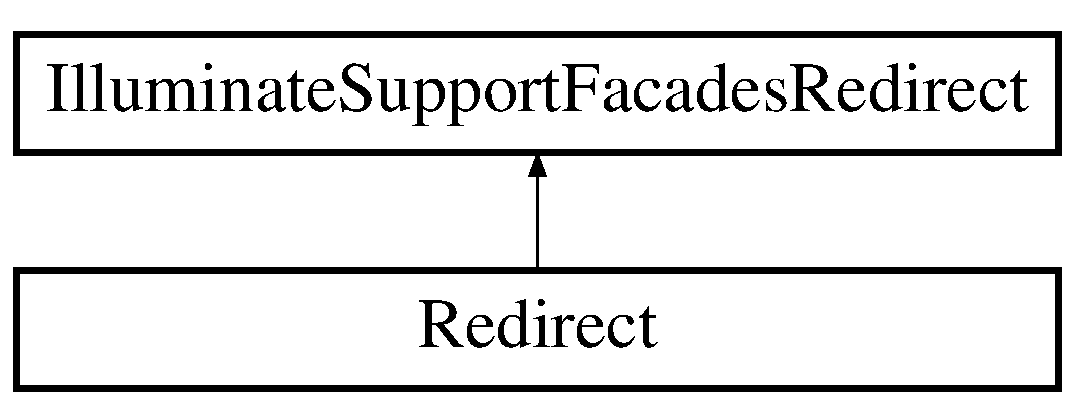
\includegraphics[height=2.000000cm]{class_illuminate_1_1_support_1_1_facades_1_1_redirect}
\end{center}
\end{figure}
\subsection*{Static Public Member Functions}
\begin{DoxyCompactItemize}
\item 
static \mbox{\hyperlink{class_illuminate_1_1_support_1_1_facades_1_1_redirect_adacf87957793d6ea7098942131255232}{home}} (\$status=302)
\item 
static \mbox{\hyperlink{class_illuminate_1_1_support_1_1_facades_1_1_redirect_a449942743abdca58f7d23ddd04110c18}{back}} (\$status=302, \$headers=array(), \$fallback=false)
\item 
static \mbox{\hyperlink{class_illuminate_1_1_support_1_1_facades_1_1_redirect_acfa54d4aec2ac31e33d601562f4eeb74}{refresh}} (\$status=302, \$headers=array())
\item 
static \mbox{\hyperlink{class_illuminate_1_1_support_1_1_facades_1_1_redirect_a91f592eb2889c431fc37134f4c36ec70}{guest}} (\$path, \$status=302, \$headers=array(), \$\mbox{\hyperlink{class_illuminate_1_1_support_1_1_facades_1_1_redirect_a6bebb89e6744dbe5100f40d584a027e4}{secure}}=null)
\item 
static \mbox{\hyperlink{class_illuminate_1_1_support_1_1_facades_1_1_redirect_ad0b6425f7fb664e0fc16216ac382a0d6}{intended}} (\$default=\textquotesingle{}/\textquotesingle{}, \$status=302, \$headers=array(), \$\mbox{\hyperlink{class_illuminate_1_1_support_1_1_facades_1_1_redirect_a6bebb89e6744dbe5100f40d584a027e4}{secure}}=null)
\item 
static \mbox{\hyperlink{class_illuminate_1_1_support_1_1_facades_1_1_redirect_aa2b771688d2c0ff2cbed8ce23b124dd3}{to}} (\$path, \$status=302, \$headers=array(), \$\mbox{\hyperlink{class_illuminate_1_1_support_1_1_facades_1_1_redirect_a6bebb89e6744dbe5100f40d584a027e4}{secure}}=null)
\item 
static \mbox{\hyperlink{class_illuminate_1_1_support_1_1_facades_1_1_redirect_a12a20d44a06b83aceefce29da7f40956}{away}} (\$path, \$status=302, \$headers=array())
\item 
static \mbox{\hyperlink{class_illuminate_1_1_support_1_1_facades_1_1_redirect_a6bebb89e6744dbe5100f40d584a027e4}{secure}} (\$path, \$status=302, \$headers=array())
\item 
static \mbox{\hyperlink{class_illuminate_1_1_support_1_1_facades_1_1_redirect_a8976d4399bdbe86aab3716e079acab0e}{route}} (\$route, \$parameters=array(), \$status=302, \$headers=array())
\item 
static \mbox{\hyperlink{class_illuminate_1_1_support_1_1_facades_1_1_redirect_a3afdcc4304c61b05589dd80783b490f7}{action}} (\$action, \$parameters=array(), \$status=302, \$headers=array())
\item 
static \mbox{\hyperlink{class_illuminate_1_1_support_1_1_facades_1_1_redirect_aadafc811c57a4418446704c6d6774bd3}{get\+Url\+Generator}} ()
\item 
static \mbox{\hyperlink{class_illuminate_1_1_support_1_1_facades_1_1_redirect_aff43d10268ae2b79c90381153dac11d1}{set\+Session}} (\$session)
\end{DoxyCompactItemize}


\subsection{Member Function Documentation}
\mbox{\Hypertarget{class_illuminate_1_1_support_1_1_facades_1_1_redirect_a3afdcc4304c61b05589dd80783b490f7}\label{class_illuminate_1_1_support_1_1_facades_1_1_redirect_a3afdcc4304c61b05589dd80783b490f7}} 
\index{Illuminate\+::\+Support\+::\+Facades\+::\+Redirect@{Illuminate\+::\+Support\+::\+Facades\+::\+Redirect}!action@{action}}
\index{action@{action}!Illuminate\+::\+Support\+::\+Facades\+::\+Redirect@{Illuminate\+::\+Support\+::\+Facades\+::\+Redirect}}
\subsubsection{\texorpdfstring{action()}{action()}}
{\footnotesize\ttfamily static Illuminate\textbackslash{}\+Support\textbackslash{}\+Facades\textbackslash{}\+Redirect\+::action (\begin{DoxyParamCaption}\item[{}]{\$action,  }\item[{}]{\$parameters = {\ttfamily array()},  }\item[{}]{\$status = {\ttfamily 302},  }\item[{}]{\$headers = {\ttfamily array()} }\end{DoxyParamCaption})\hspace{0.3cm}{\ttfamily [static]}}

Create a new redirect response to a controller action.


\begin{DoxyParams}[1]{Parameters}
string & {\em \$action} & \\
\hline
array & {\em \$parameters} & \\
\hline
int & {\em \$status} & \\
\hline
array & {\em \$headers} & \\
\hline
\end{DoxyParams}
\begin{DoxyReturn}{Returns}

\end{DoxyReturn}
\mbox{\Hypertarget{class_illuminate_1_1_support_1_1_facades_1_1_redirect_a12a20d44a06b83aceefce29da7f40956}\label{class_illuminate_1_1_support_1_1_facades_1_1_redirect_a12a20d44a06b83aceefce29da7f40956}} 
\index{Illuminate\+::\+Support\+::\+Facades\+::\+Redirect@{Illuminate\+::\+Support\+::\+Facades\+::\+Redirect}!away@{away}}
\index{away@{away}!Illuminate\+::\+Support\+::\+Facades\+::\+Redirect@{Illuminate\+::\+Support\+::\+Facades\+::\+Redirect}}
\subsubsection{\texorpdfstring{away()}{away()}}
{\footnotesize\ttfamily static Illuminate\textbackslash{}\+Support\textbackslash{}\+Facades\textbackslash{}\+Redirect\+::away (\begin{DoxyParamCaption}\item[{}]{\$path,  }\item[{}]{\$status = {\ttfamily 302},  }\item[{}]{\$headers = {\ttfamily array()} }\end{DoxyParamCaption})\hspace{0.3cm}{\ttfamily [static]}}

Create a new redirect response to an external \mbox{\hyperlink{class_illuminate_1_1_support_1_1_facades_1_1_u_r_l}{U\+RL}} (no validation).


\begin{DoxyParams}[1]{Parameters}
string & {\em \$path} & \\
\hline
int & {\em \$status} & \\
\hline
array & {\em \$headers} & \\
\hline
\end{DoxyParams}
\begin{DoxyReturn}{Returns}

\end{DoxyReturn}
\mbox{\Hypertarget{class_illuminate_1_1_support_1_1_facades_1_1_redirect_a449942743abdca58f7d23ddd04110c18}\label{class_illuminate_1_1_support_1_1_facades_1_1_redirect_a449942743abdca58f7d23ddd04110c18}} 
\index{Illuminate\+::\+Support\+::\+Facades\+::\+Redirect@{Illuminate\+::\+Support\+::\+Facades\+::\+Redirect}!back@{back}}
\index{back@{back}!Illuminate\+::\+Support\+::\+Facades\+::\+Redirect@{Illuminate\+::\+Support\+::\+Facades\+::\+Redirect}}
\subsubsection{\texorpdfstring{back()}{back()}}
{\footnotesize\ttfamily static Illuminate\textbackslash{}\+Support\textbackslash{}\+Facades\textbackslash{}\+Redirect\+::back (\begin{DoxyParamCaption}\item[{}]{\$status = {\ttfamily 302},  }\item[{}]{\$headers = {\ttfamily array()},  }\item[{}]{\$fallback = {\ttfamily false} }\end{DoxyParamCaption})\hspace{0.3cm}{\ttfamily [static]}}

Create a new redirect response to the previous location.


\begin{DoxyParams}[1]{Parameters}
int & {\em \$status} & \\
\hline
array & {\em \$headers} & \\
\hline
mixed & {\em \$fallback} & \\
\hline
\end{DoxyParams}
\begin{DoxyReturn}{Returns}

\end{DoxyReturn}
\mbox{\Hypertarget{class_illuminate_1_1_support_1_1_facades_1_1_redirect_aadafc811c57a4418446704c6d6774bd3}\label{class_illuminate_1_1_support_1_1_facades_1_1_redirect_aadafc811c57a4418446704c6d6774bd3}} 
\index{Illuminate\+::\+Support\+::\+Facades\+::\+Redirect@{Illuminate\+::\+Support\+::\+Facades\+::\+Redirect}!get\+Url\+Generator@{get\+Url\+Generator}}
\index{get\+Url\+Generator@{get\+Url\+Generator}!Illuminate\+::\+Support\+::\+Facades\+::\+Redirect@{Illuminate\+::\+Support\+::\+Facades\+::\+Redirect}}
\subsubsection{\texorpdfstring{get\+Url\+Generator()}{getUrlGenerator()}}
{\footnotesize\ttfamily static Illuminate\textbackslash{}\+Support\textbackslash{}\+Facades\textbackslash{}\+Redirect\+::get\+Url\+Generator (\begin{DoxyParamCaption}{ }\end{DoxyParamCaption})\hspace{0.3cm}{\ttfamily [static]}}

Get the \mbox{\hyperlink{class_illuminate_1_1_support_1_1_facades_1_1_u_r_l}{U\+RL}} generator instance.

\begin{DoxyReturn}{Returns}

\end{DoxyReturn}
\mbox{\Hypertarget{class_illuminate_1_1_support_1_1_facades_1_1_redirect_a91f592eb2889c431fc37134f4c36ec70}\label{class_illuminate_1_1_support_1_1_facades_1_1_redirect_a91f592eb2889c431fc37134f4c36ec70}} 
\index{Illuminate\+::\+Support\+::\+Facades\+::\+Redirect@{Illuminate\+::\+Support\+::\+Facades\+::\+Redirect}!guest@{guest}}
\index{guest@{guest}!Illuminate\+::\+Support\+::\+Facades\+::\+Redirect@{Illuminate\+::\+Support\+::\+Facades\+::\+Redirect}}
\subsubsection{\texorpdfstring{guest()}{guest()}}
{\footnotesize\ttfamily static Illuminate\textbackslash{}\+Support\textbackslash{}\+Facades\textbackslash{}\+Redirect\+::guest (\begin{DoxyParamCaption}\item[{}]{\$path,  }\item[{}]{\$status = {\ttfamily 302},  }\item[{}]{\$headers = {\ttfamily array()},  }\item[{}]{\$secure = {\ttfamily null} }\end{DoxyParamCaption})\hspace{0.3cm}{\ttfamily [static]}}

Create a new redirect response, while putting the current \mbox{\hyperlink{class_illuminate_1_1_support_1_1_facades_1_1_u_r_l}{U\+RL}} in the session.


\begin{DoxyParams}[1]{Parameters}
string & {\em \$path} & \\
\hline
int & {\em \$status} & \\
\hline
array & {\em \$headers} & \\
\hline
bool & {\em \$secure} & \\
\hline
\end{DoxyParams}
\begin{DoxyReturn}{Returns}

\end{DoxyReturn}
\mbox{\Hypertarget{class_illuminate_1_1_support_1_1_facades_1_1_redirect_adacf87957793d6ea7098942131255232}\label{class_illuminate_1_1_support_1_1_facades_1_1_redirect_adacf87957793d6ea7098942131255232}} 
\index{Illuminate\+::\+Support\+::\+Facades\+::\+Redirect@{Illuminate\+::\+Support\+::\+Facades\+::\+Redirect}!home@{home}}
\index{home@{home}!Illuminate\+::\+Support\+::\+Facades\+::\+Redirect@{Illuminate\+::\+Support\+::\+Facades\+::\+Redirect}}
\subsubsection{\texorpdfstring{home()}{home()}}
{\footnotesize\ttfamily static Illuminate\textbackslash{}\+Support\textbackslash{}\+Facades\textbackslash{}\+Redirect\+::home (\begin{DoxyParamCaption}\item[{}]{\$status = {\ttfamily 302} }\end{DoxyParamCaption})\hspace{0.3cm}{\ttfamily [static]}}

Create a new redirect response to the \char`\"{}home\char`\"{} route.


\begin{DoxyParams}[1]{Parameters}
int & {\em \$status} & \\
\hline
\end{DoxyParams}
\begin{DoxyReturn}{Returns}

\end{DoxyReturn}
\mbox{\Hypertarget{class_illuminate_1_1_support_1_1_facades_1_1_redirect_ad0b6425f7fb664e0fc16216ac382a0d6}\label{class_illuminate_1_1_support_1_1_facades_1_1_redirect_ad0b6425f7fb664e0fc16216ac382a0d6}} 
\index{Illuminate\+::\+Support\+::\+Facades\+::\+Redirect@{Illuminate\+::\+Support\+::\+Facades\+::\+Redirect}!intended@{intended}}
\index{intended@{intended}!Illuminate\+::\+Support\+::\+Facades\+::\+Redirect@{Illuminate\+::\+Support\+::\+Facades\+::\+Redirect}}
\subsubsection{\texorpdfstring{intended()}{intended()}}
{\footnotesize\ttfamily static Illuminate\textbackslash{}\+Support\textbackslash{}\+Facades\textbackslash{}\+Redirect\+::intended (\begin{DoxyParamCaption}\item[{}]{\$default = {\ttfamily \textquotesingle{}/\textquotesingle{}},  }\item[{}]{\$status = {\ttfamily 302},  }\item[{}]{\$headers = {\ttfamily array()},  }\item[{}]{\$secure = {\ttfamily null} }\end{DoxyParamCaption})\hspace{0.3cm}{\ttfamily [static]}}

Create a new redirect response to the previously intended location.


\begin{DoxyParams}[1]{Parameters}
string & {\em \$default} & \\
\hline
int & {\em \$status} & \\
\hline
array & {\em \$headers} & \\
\hline
bool & {\em \$secure} & \\
\hline
\end{DoxyParams}
\begin{DoxyReturn}{Returns}

\end{DoxyReturn}
\mbox{\Hypertarget{class_illuminate_1_1_support_1_1_facades_1_1_redirect_acfa54d4aec2ac31e33d601562f4eeb74}\label{class_illuminate_1_1_support_1_1_facades_1_1_redirect_acfa54d4aec2ac31e33d601562f4eeb74}} 
\index{Illuminate\+::\+Support\+::\+Facades\+::\+Redirect@{Illuminate\+::\+Support\+::\+Facades\+::\+Redirect}!refresh@{refresh}}
\index{refresh@{refresh}!Illuminate\+::\+Support\+::\+Facades\+::\+Redirect@{Illuminate\+::\+Support\+::\+Facades\+::\+Redirect}}
\subsubsection{\texorpdfstring{refresh()}{refresh()}}
{\footnotesize\ttfamily static Illuminate\textbackslash{}\+Support\textbackslash{}\+Facades\textbackslash{}\+Redirect\+::refresh (\begin{DoxyParamCaption}\item[{}]{\$status = {\ttfamily 302},  }\item[{}]{\$headers = {\ttfamily array()} }\end{DoxyParamCaption})\hspace{0.3cm}{\ttfamily [static]}}

Create a new redirect response to the current U\+RI.


\begin{DoxyParams}[1]{Parameters}
int & {\em \$status} & \\
\hline
array & {\em \$headers} & \\
\hline
\end{DoxyParams}
\begin{DoxyReturn}{Returns}

\end{DoxyReturn}
\mbox{\Hypertarget{class_illuminate_1_1_support_1_1_facades_1_1_redirect_a8976d4399bdbe86aab3716e079acab0e}\label{class_illuminate_1_1_support_1_1_facades_1_1_redirect_a8976d4399bdbe86aab3716e079acab0e}} 
\index{Illuminate\+::\+Support\+::\+Facades\+::\+Redirect@{Illuminate\+::\+Support\+::\+Facades\+::\+Redirect}!route@{route}}
\index{route@{route}!Illuminate\+::\+Support\+::\+Facades\+::\+Redirect@{Illuminate\+::\+Support\+::\+Facades\+::\+Redirect}}
\subsubsection{\texorpdfstring{route()}{route()}}
{\footnotesize\ttfamily static Illuminate\textbackslash{}\+Support\textbackslash{}\+Facades\textbackslash{}\+Redirect\+::route (\begin{DoxyParamCaption}\item[{}]{\$route,  }\item[{}]{\$parameters = {\ttfamily array()},  }\item[{}]{\$status = {\ttfamily 302},  }\item[{}]{\$headers = {\ttfamily array()} }\end{DoxyParamCaption})\hspace{0.3cm}{\ttfamily [static]}}

Create a new redirect response to a named route.


\begin{DoxyParams}[1]{Parameters}
string & {\em \$route} & \\
\hline
array & {\em \$parameters} & \\
\hline
int & {\em \$status} & \\
\hline
array & {\em \$headers} & \\
\hline
\end{DoxyParams}
\begin{DoxyReturn}{Returns}

\end{DoxyReturn}
\mbox{\Hypertarget{class_illuminate_1_1_support_1_1_facades_1_1_redirect_a6bebb89e6744dbe5100f40d584a027e4}\label{class_illuminate_1_1_support_1_1_facades_1_1_redirect_a6bebb89e6744dbe5100f40d584a027e4}} 
\index{Illuminate\+::\+Support\+::\+Facades\+::\+Redirect@{Illuminate\+::\+Support\+::\+Facades\+::\+Redirect}!secure@{secure}}
\index{secure@{secure}!Illuminate\+::\+Support\+::\+Facades\+::\+Redirect@{Illuminate\+::\+Support\+::\+Facades\+::\+Redirect}}
\subsubsection{\texorpdfstring{secure()}{secure()}}
{\footnotesize\ttfamily static Illuminate\textbackslash{}\+Support\textbackslash{}\+Facades\textbackslash{}\+Redirect\+::secure (\begin{DoxyParamCaption}\item[{}]{\$path,  }\item[{}]{\$status = {\ttfamily 302},  }\item[{}]{\$headers = {\ttfamily array()} }\end{DoxyParamCaption})\hspace{0.3cm}{\ttfamily [static]}}

Create a new redirect response to the given H\+T\+T\+PS path.


\begin{DoxyParams}[1]{Parameters}
string & {\em \$path} & \\
\hline
int & {\em \$status} & \\
\hline
array & {\em \$headers} & \\
\hline
\end{DoxyParams}
\begin{DoxyReturn}{Returns}

\end{DoxyReturn}
\mbox{\Hypertarget{class_illuminate_1_1_support_1_1_facades_1_1_redirect_aff43d10268ae2b79c90381153dac11d1}\label{class_illuminate_1_1_support_1_1_facades_1_1_redirect_aff43d10268ae2b79c90381153dac11d1}} 
\index{Illuminate\+::\+Support\+::\+Facades\+::\+Redirect@{Illuminate\+::\+Support\+::\+Facades\+::\+Redirect}!set\+Session@{set\+Session}}
\index{set\+Session@{set\+Session}!Illuminate\+::\+Support\+::\+Facades\+::\+Redirect@{Illuminate\+::\+Support\+::\+Facades\+::\+Redirect}}
\subsubsection{\texorpdfstring{set\+Session()}{setSession()}}
{\footnotesize\ttfamily static Illuminate\textbackslash{}\+Support\textbackslash{}\+Facades\textbackslash{}\+Redirect\+::set\+Session (\begin{DoxyParamCaption}\item[{}]{\$session }\end{DoxyParamCaption})\hspace{0.3cm}{\ttfamily [static]}}

Set the active session store.


\begin{DoxyParams}[1]{Parameters}
\textbackslash{}\+Illuminate\textbackslash{}\+Session\textbackslash{}\+Store & {\em \$session} & \\
\hline
\end{DoxyParams}
\begin{DoxyReturn}{Returns}
void 
\end{DoxyReturn}
\mbox{\Hypertarget{class_illuminate_1_1_support_1_1_facades_1_1_redirect_aa2b771688d2c0ff2cbed8ce23b124dd3}\label{class_illuminate_1_1_support_1_1_facades_1_1_redirect_aa2b771688d2c0ff2cbed8ce23b124dd3}} 
\index{Illuminate\+::\+Support\+::\+Facades\+::\+Redirect@{Illuminate\+::\+Support\+::\+Facades\+::\+Redirect}!to@{to}}
\index{to@{to}!Illuminate\+::\+Support\+::\+Facades\+::\+Redirect@{Illuminate\+::\+Support\+::\+Facades\+::\+Redirect}}
\subsubsection{\texorpdfstring{to()}{to()}}
{\footnotesize\ttfamily static Illuminate\textbackslash{}\+Support\textbackslash{}\+Facades\textbackslash{}\+Redirect\+::to (\begin{DoxyParamCaption}\item[{}]{\$path,  }\item[{}]{\$status = {\ttfamily 302},  }\item[{}]{\$headers = {\ttfamily array()},  }\item[{}]{\$secure = {\ttfamily null} }\end{DoxyParamCaption})\hspace{0.3cm}{\ttfamily [static]}}

Create a new redirect response to the given path.


\begin{DoxyParams}[1]{Parameters}
string & {\em \$path} & \\
\hline
int & {\em \$status} & \\
\hline
array & {\em \$headers} & \\
\hline
bool & {\em \$secure} & \\
\hline
\end{DoxyParams}
\begin{DoxyReturn}{Returns}

\end{DoxyReturn}


The documentation for this class was generated from the following file\+:\begin{DoxyCompactItemize}
\item 
\+\_\+ide\+\_\+helper.\+php\end{DoxyCompactItemize}

\hypertarget{class_redirect}{}\section{Redirect Class Reference}
\label{class_redirect}\index{Redirect@{Redirect}}
Inheritance diagram for Redirect\+:\begin{figure}[H]
\begin{center}
\leavevmode
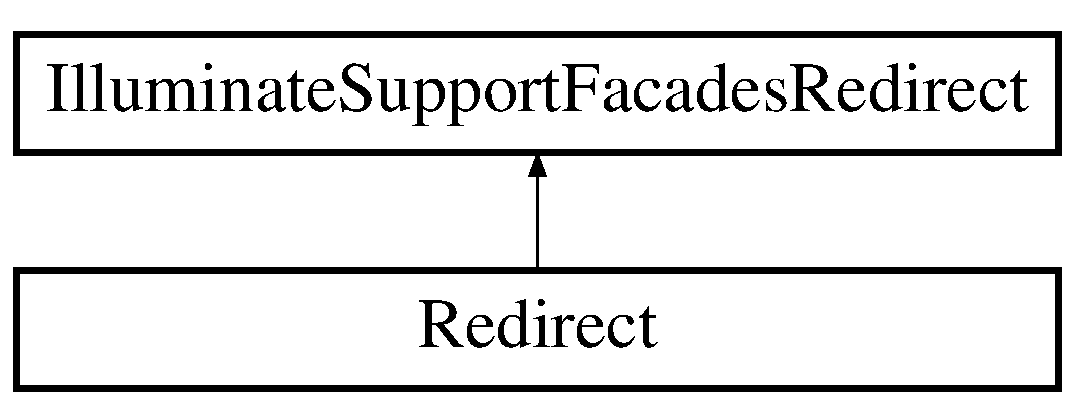
\includegraphics[height=2.000000cm]{class_redirect}
\end{center}
\end{figure}
\subsection*{Additional Inherited Members}


The documentation for this class was generated from the following file\+:\begin{DoxyCompactItemize}
\item 
\+\_\+ide\+\_\+helper.\+php\end{DoxyCompactItemize}

\hypertarget{class_request}{}\section{Request Class Reference}
\label{class_request}\index{Request@{Request}}
Inheritance diagram for Request\+:\begin{figure}[H]
\begin{center}
\leavevmode
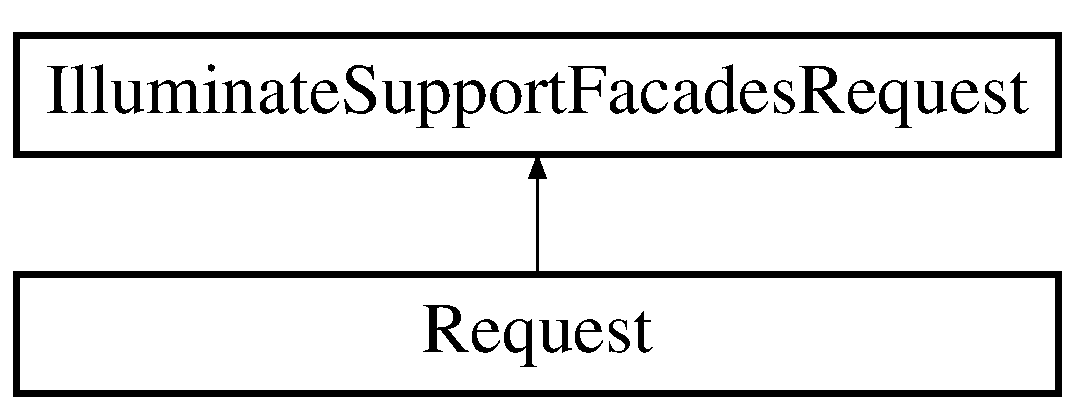
\includegraphics[height=2.000000cm]{class_request}
\end{center}
\end{figure}
\subsection*{Additional Inherited Members}


The documentation for this class was generated from the following file\+:\begin{DoxyCompactItemize}
\item 
\+\_\+ide\+\_\+helper.\+php\end{DoxyCompactItemize}

\hypertarget{class_illuminate_1_1_support_1_1_facades_1_1_request}{}\section{Illuminate\textbackslash{}Support\textbackslash{}Facades\textbackslash{}Request Class Reference}
\label{class_illuminate_1_1_support_1_1_facades_1_1_request}\index{Illuminate\textbackslash{}\+Support\textbackslash{}\+Facades\textbackslash{}\+Request@{Illuminate\textbackslash{}\+Support\textbackslash{}\+Facades\textbackslash{}\+Request}}
Inheritance diagram for Illuminate\textbackslash{}Support\textbackslash{}Facades\textbackslash{}Request\+:\begin{figure}[H]
\begin{center}
\leavevmode
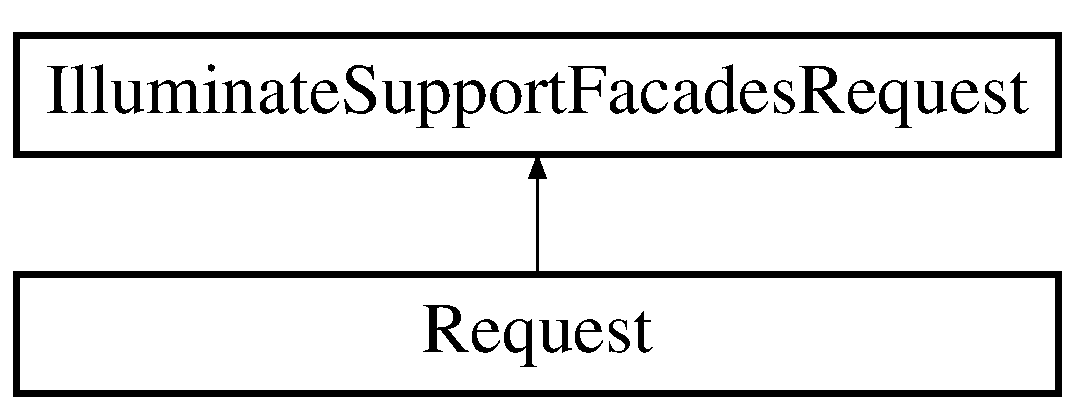
\includegraphics[height=2.000000cm]{class_illuminate_1_1_support_1_1_facades_1_1_request}
\end{center}
\end{figure}
\subsection*{Static Public Member Functions}
\begin{DoxyCompactItemize}
\item 
static \mbox{\hyperlink{class_illuminate_1_1_support_1_1_facades_1_1_request_a04c59f7a4652190ee9b815a246d4d030}{capture}} ()
\item 
static \mbox{\hyperlink{class_illuminate_1_1_support_1_1_facades_1_1_request_a46303e78a0876d7bba541b64581aec66}{instance}} ()
\item 
static \mbox{\hyperlink{class_illuminate_1_1_support_1_1_facades_1_1_request_af4fe38392dfdd7f5daa7d2d811bad24d}{method}} ()
\item 
static \mbox{\hyperlink{class_illuminate_1_1_support_1_1_facades_1_1_request_a49120cc9c3ade50c8d5ede20c186a1a4}{root}} ()
\item 
static \mbox{\hyperlink{class_illuminate_1_1_support_1_1_facades_1_1_request_a2989a827618b1759471556aaacfe446f}{url}} ()
\item 
static \mbox{\hyperlink{class_illuminate_1_1_support_1_1_facades_1_1_request_a45110aa4e3e4f712691453fd39a241e0}{full\+Url}} ()
\item 
static \mbox{\hyperlink{class_illuminate_1_1_support_1_1_facades_1_1_request_a078d7acddf08cbc6d1b71efcdbebcde6}{full\+Url\+With\+Query}} (\$\mbox{\hyperlink{class_illuminate_1_1_support_1_1_facades_1_1_request_abaa6d157fd299de004ac80239a11aa5a}{query}})
\item 
static \mbox{\hyperlink{class_illuminate_1_1_support_1_1_facades_1_1_request_ad288b957470d9cdb3b2b35c65c6e7a4c}{path}} ()
\item 
static \mbox{\hyperlink{class_illuminate_1_1_support_1_1_facades_1_1_request_a5ef76eb084577dcaeb0f17dac3b13192}{decoded\+Path}} ()
\item 
static \mbox{\hyperlink{class_illuminate_1_1_support_1_1_facades_1_1_request_a860203430647b4261b5ecbdd04242dd0}{segment}} (\$index, \$default=null)
\item 
static \mbox{\hyperlink{class_illuminate_1_1_support_1_1_facades_1_1_request_ad63ac5bdb7a81ce91043fda9e7e88685}{segments}} ()
\item 
static \mbox{\hyperlink{class_illuminate_1_1_support_1_1_facades_1_1_request_aee3d15739be982a658320ac868c16a43}{is}} (\$patterns=null)
\item 
static \mbox{\hyperlink{class_illuminate_1_1_support_1_1_facades_1_1_request_a3d91ee547365fbae69326d4331b12457}{route\+Is}} (\$patterns=null)
\item 
static \mbox{\hyperlink{class_illuminate_1_1_support_1_1_facades_1_1_request_aa19fd01c7be2110f177b8cff6559efb2}{full\+Url\+Is}} (\$patterns=null)
\item 
static \mbox{\hyperlink{class_illuminate_1_1_support_1_1_facades_1_1_request_aecead1bc0512dadbebbf5e7aa74b2544}{ajax}} ()
\item 
static \mbox{\hyperlink{class_illuminate_1_1_support_1_1_facades_1_1_request_ab38ddcb23db31c0bc23ea576e28d868d}{pjax}} ()
\item 
static \mbox{\hyperlink{class_illuminate_1_1_support_1_1_facades_1_1_request_a80f6609d3acb22116e64c05d6e0ecfb9}{secure}} ()
\item 
static \mbox{\hyperlink{class_illuminate_1_1_support_1_1_facades_1_1_request_a4c0dc61a627ddae9c7c3ec74d845e483}{ip}} ()
\item 
static \mbox{\hyperlink{class_illuminate_1_1_support_1_1_facades_1_1_request_a907a99501b1a1f7a8349e71a5a51ee2b}{ips}} ()
\item 
static \mbox{\hyperlink{class_illuminate_1_1_support_1_1_facades_1_1_request_a3a185583cec2b7eefae89f509cb4f3ab}{user\+Agent}} ()
\item 
static \mbox{\hyperlink{class_illuminate_1_1_support_1_1_facades_1_1_request_a184ac93e1b0ebb5c9bd720a6bad67e95}{merge}} (\$\mbox{\hyperlink{class_illuminate_1_1_support_1_1_facades_1_1_request_a9ce57d739a5036919120eb369d80dd7a}{input}})
\item 
static \mbox{\hyperlink{class_illuminate_1_1_support_1_1_facades_1_1_request_a3d323a9c8ad910a8eb27ba08116eaf0b}{replace}} (\$\mbox{\hyperlink{class_illuminate_1_1_support_1_1_facades_1_1_request_a9ce57d739a5036919120eb369d80dd7a}{input}})
\item 
static \mbox{\hyperlink{class_illuminate_1_1_support_1_1_facades_1_1_request_ad03fe88fc6916a4a2a1a9f3da85bdc77}{json}} (\$key=null, \$default=null)
\item 
static \mbox{\hyperlink{class_illuminate_1_1_support_1_1_facades_1_1_request_aeda33757e75030fdc25f1c17afcc74d4}{create\+From\+Base}} (\$request)
\item 
static \mbox{\hyperlink{class_illuminate_1_1_support_1_1_facades_1_1_request_a811172c986cdc6ecc7cf8801bcdc6eb9}{duplicate}} (\$\mbox{\hyperlink{class_illuminate_1_1_support_1_1_facades_1_1_request_abaa6d157fd299de004ac80239a11aa5a}{query}}=null, \$request=null, \$attributes=null, \$cookies=null, \$files=null, \$\mbox{\hyperlink{class_illuminate_1_1_support_1_1_facades_1_1_request_aaea79f85875a529d365d560bde09bf16}{server}}=null)
\item 
static \mbox{\hyperlink{class_illuminate_1_1_support_1_1_facades_1_1_request_a3b3b1c25368c2e40ecdb0830a53183a8}{session}} ()
\item 
static \mbox{\hyperlink{class_illuminate_1_1_support_1_1_facades_1_1_request_afa28362d11bfebad752f6d684ee4dd8c}{set\+Laravel\+Session}} (\$\mbox{\hyperlink{class_illuminate_1_1_support_1_1_facades_1_1_request_a3b3b1c25368c2e40ecdb0830a53183a8}{session}})
\item 
static \mbox{\hyperlink{class_illuminate_1_1_support_1_1_facades_1_1_request_ae16165d7bff8e8c3b2a1c8c58e59e719}{user}} (\$guard=null)
\item 
static \mbox{\hyperlink{class_illuminate_1_1_support_1_1_facades_1_1_request_abf913e2bc3550d8804377ed6aed93be4}{route}} (\$param=null)
\item 
static \mbox{\hyperlink{class_illuminate_1_1_support_1_1_facades_1_1_request_a8bc9e7cd157d79c8fb32f2933148ac14}{fingerprint}} ()
\item 
static \mbox{\hyperlink{class_illuminate_1_1_support_1_1_facades_1_1_request_aaa19d5acec04b37afa4f6369d9276c54}{set\+Json}} (\$\mbox{\hyperlink{class_illuminate_1_1_support_1_1_facades_1_1_request_ad03fe88fc6916a4a2a1a9f3da85bdc77}{json}})
\item 
static \mbox{\hyperlink{class_illuminate_1_1_support_1_1_facades_1_1_request_a8833d40ed5180cb3c3a712c131f8ff7b}{get\+User\+Resolver}} ()
\item 
static \mbox{\hyperlink{class_illuminate_1_1_support_1_1_facades_1_1_request_a3d4ed4ec038935ba3db9a690184ede58}{set\+User\+Resolver}} (\$callback)
\item 
static \mbox{\hyperlink{class_illuminate_1_1_support_1_1_facades_1_1_request_a1f2c14881d3d33998ced0a661e2c1349}{get\+Route\+Resolver}} ()
\item 
static \mbox{\hyperlink{class_illuminate_1_1_support_1_1_facades_1_1_request_a5fb4b7d38a7b75fc2dea8ea36d8f3f56}{set\+Route\+Resolver}} (\$callback)
\item 
static \mbox{\hyperlink{class_illuminate_1_1_support_1_1_facades_1_1_request_ad2100d4f15a188ccce3dd8a9ec885389}{to\+Array}} ()
\item 
static \mbox{\hyperlink{class_illuminate_1_1_support_1_1_facades_1_1_request_a846e51a1bad906d0b7dc34149d24b5da}{offset\+Exists}} (\$offset)
\item 
static \mbox{\hyperlink{class_illuminate_1_1_support_1_1_facades_1_1_request_a5e9324bd92c95487e0e2d4c9e2fac814}{offset\+Get}} (\$offset)
\item 
static \mbox{\hyperlink{class_illuminate_1_1_support_1_1_facades_1_1_request_a152259a20338648884c97f30fceebec3}{offset\+Set}} (\$offset, \$value)
\item 
static \mbox{\hyperlink{class_illuminate_1_1_support_1_1_facades_1_1_request_a0a1207e664392d43d200cbcf94f0ecee}{offset\+Unset}} (\$offset)
\item 
static \mbox{\hyperlink{class_illuminate_1_1_support_1_1_facades_1_1_request_a48b56a8b2a03a51267ac34fd60d90766}{initialize}} (\$\mbox{\hyperlink{class_illuminate_1_1_support_1_1_facades_1_1_request_abaa6d157fd299de004ac80239a11aa5a}{query}}=array(), \$request=array(), \$attributes=array(), \$cookies=array(), \$files=array(), \$\mbox{\hyperlink{class_illuminate_1_1_support_1_1_facades_1_1_request_aaea79f85875a529d365d560bde09bf16}{server}}=array(), \$content=null)
\item 
static \mbox{\hyperlink{class_illuminate_1_1_support_1_1_facades_1_1_request_a09634cd14effd077c44a779500b8ff2c}{create\+From\+Globals}} ()
\item 
static \mbox{\hyperlink{class_illuminate_1_1_support_1_1_facades_1_1_request_a342ea9db43861f8dd293ff94bfa6b795}{create}} (\$uri, \$\mbox{\hyperlink{class_illuminate_1_1_support_1_1_facades_1_1_request_af4fe38392dfdd7f5daa7d2d811bad24d}{method}}=\textquotesingle{}G\+ET\textquotesingle{}, \$parameters=array(), \$cookies=array(), \$files=array(), \$\mbox{\hyperlink{class_illuminate_1_1_support_1_1_facades_1_1_request_aaea79f85875a529d365d560bde09bf16}{server}}=array(), \$content=null)
\item 
static \mbox{\hyperlink{class_illuminate_1_1_support_1_1_facades_1_1_request_a223c49b4b59ee06341172efbd2362139}{set\+Factory}} (\$callable)
\item 
static \mbox{\hyperlink{class_illuminate_1_1_support_1_1_facades_1_1_request_afd2c5e18dcee250f7de186821bf7afab}{override\+Globals}} ()
\item 
static \mbox{\hyperlink{class_illuminate_1_1_support_1_1_facades_1_1_request_a1686fbcf12f72ed06a19adf0633054fa}{set\+Trusted\+Proxies}} (\$proxies)
\item 
static \mbox{\hyperlink{class_illuminate_1_1_support_1_1_facades_1_1_request_ae27082de42e9584c5b87d6f4db424e2c}{get\+Trusted\+Proxies}} ()
\item 
static \mbox{\hyperlink{class_illuminate_1_1_support_1_1_facades_1_1_request_ae3ef3d27cc0d73a108b3f97e4568bd76}{get\+Trusted\+Header\+Set}} ()
\item 
static \mbox{\hyperlink{class_illuminate_1_1_support_1_1_facades_1_1_request_a0f4e03016975d5e78f6841b4b3b2d853}{set\+Trusted\+Hosts}} (\$host\+Patterns)
\item 
static \mbox{\hyperlink{class_illuminate_1_1_support_1_1_facades_1_1_request_a7af20f1cdde18bc998466e6b94613503}{get\+Trusted\+Hosts}} ()
\item 
static \mbox{\hyperlink{class_illuminate_1_1_support_1_1_facades_1_1_request_abbd0aa91652f2122be7a351876da3468}{set\+Trusted\+Header\+Name}} (\$key, \$value)
\item 
static \mbox{\hyperlink{class_illuminate_1_1_support_1_1_facades_1_1_request_a55370a6f7198b65ee1ab0f8416f4fb40}{get\+Trusted\+Header\+Name}} (\$key)
\item 
static \mbox{\hyperlink{class_illuminate_1_1_support_1_1_facades_1_1_request_a4e65d88d0e7c68e2b9aaafcfe83a91b5}{normalize\+Query\+String}} (\$qs)
\item 
static \mbox{\hyperlink{class_illuminate_1_1_support_1_1_facades_1_1_request_a39cf798202cb88125c454d7813767a01}{enable\+Http\+Method\+Parameter\+Override}} ()
\item 
static \mbox{\hyperlink{class_illuminate_1_1_support_1_1_facades_1_1_request_a6dc526d395a74c75de55eb597cbf66d5}{get\+Http\+Method\+Parameter\+Override}} ()
\item 
static \mbox{\hyperlink{class_illuminate_1_1_support_1_1_facades_1_1_request_af1519e8f3d8baaa19829f3f4a53c9b41}{get}} (\$key, \$default=null)
\item 
static \mbox{\hyperlink{class_illuminate_1_1_support_1_1_facades_1_1_request_a19c092888199ad4b1e3e5f254bc65698}{get\+Session}} ()
\item 
static \mbox{\hyperlink{class_illuminate_1_1_support_1_1_facades_1_1_request_a70640b694c1a135a6e196be88478c25f}{has\+Previous\+Session}} ()
\item 
static \mbox{\hyperlink{class_illuminate_1_1_support_1_1_facades_1_1_request_abdb40f9f98e0988e0d46701d84b08eaa}{has\+Session}} ()
\item 
static \mbox{\hyperlink{class_illuminate_1_1_support_1_1_facades_1_1_request_a89fade31642421bad06c770d5d3505fa}{set\+Session}} (\$\mbox{\hyperlink{class_illuminate_1_1_support_1_1_facades_1_1_request_a3b3b1c25368c2e40ecdb0830a53183a8}{session}})
\item 
static \mbox{\hyperlink{class_illuminate_1_1_support_1_1_facades_1_1_request_acff1ecb5fd2edd0194bfa8ab1c120bcd}{get\+Client\+Ips}} ()
\item 
static \mbox{\hyperlink{class_illuminate_1_1_support_1_1_facades_1_1_request_ac78e7218a697e138ce105a04d49f2ff7}{get\+Client\+Ip}} ()
\item 
static \mbox{\hyperlink{class_illuminate_1_1_support_1_1_facades_1_1_request_abbaae1eb9e945968ecf88a6028fdad1d}{get\+Script\+Name}} ()
\item 
static \mbox{\hyperlink{class_illuminate_1_1_support_1_1_facades_1_1_request_a338cf633d5763b7456ab6caa5cde0168}{get\+Path\+Info}} ()
\item 
static \mbox{\hyperlink{class_illuminate_1_1_support_1_1_facades_1_1_request_a7ff313f9f7aa4c84a15e5f5378ea0b6f}{get\+Base\+Path}} ()
\item 
static \mbox{\hyperlink{class_illuminate_1_1_support_1_1_facades_1_1_request_a8aa479bbfa1d5f2e34b783561a674ee9}{get\+Base\+Url}} ()
\item 
static \mbox{\hyperlink{class_illuminate_1_1_support_1_1_facades_1_1_request_ab575d7512ffc8d22cf2f3facfaee0065}{get\+Scheme}} ()
\item 
static \mbox{\hyperlink{class_illuminate_1_1_support_1_1_facades_1_1_request_afc28cdf3fdcae21e6c5d0596b041c5e8}{get\+Port}} ()
\item 
static \mbox{\hyperlink{class_illuminate_1_1_support_1_1_facades_1_1_request_af6be07fd0431be5d0a2e28c874d7a39c}{get\+User}} ()
\item 
static \mbox{\hyperlink{class_illuminate_1_1_support_1_1_facades_1_1_request_a3a532c73c1fc35755642cb93c47098af}{get\+Password}} ()
\item 
static \mbox{\hyperlink{class_illuminate_1_1_support_1_1_facades_1_1_request_a8ce2186aaa9ce132b469fd8e61b20a5e}{get\+User\+Info}} ()
\item 
static \mbox{\hyperlink{class_illuminate_1_1_support_1_1_facades_1_1_request_a94046dd08b0253ae63caf787fd1f9d80}{get\+Http\+Host}} ()
\item 
static \mbox{\hyperlink{class_illuminate_1_1_support_1_1_facades_1_1_request_a91b1026ed524e8ece81eb56e47721256}{get\+Request\+Uri}} ()
\item 
static \mbox{\hyperlink{class_illuminate_1_1_support_1_1_facades_1_1_request_a6576e102a6c46aaf0a0167c7b45a51f5}{get\+Scheme\+And\+Http\+Host}} ()
\item 
static \mbox{\hyperlink{class_illuminate_1_1_support_1_1_facades_1_1_request_a981fe9da5324bee9feb4664b5b574e87}{get\+Uri}} ()
\item 
static \mbox{\hyperlink{class_illuminate_1_1_support_1_1_facades_1_1_request_a5f9581e38f5a7609b62f7fa4b1bd1116}{get\+Uri\+For\+Path}} (\$\mbox{\hyperlink{class_illuminate_1_1_support_1_1_facades_1_1_request_ad288b957470d9cdb3b2b35c65c6e7a4c}{path}})
\item 
static \mbox{\hyperlink{class_illuminate_1_1_support_1_1_facades_1_1_request_ac3134c844be4a9bf63a2f5e9153e0b0d}{get\+Relative\+Uri\+For\+Path}} (\$\mbox{\hyperlink{class_illuminate_1_1_support_1_1_facades_1_1_request_ad288b957470d9cdb3b2b35c65c6e7a4c}{path}})
\item 
static \mbox{\hyperlink{class_illuminate_1_1_support_1_1_facades_1_1_request_aec1fe0b0a5b7c90b9b3606f967083d82}{get\+Query\+String}} ()
\item 
static \mbox{\hyperlink{class_illuminate_1_1_support_1_1_facades_1_1_request_a9a401927e509ddb652b5656407b37bf2}{is\+Secure}} ()
\item 
static \mbox{\hyperlink{class_illuminate_1_1_support_1_1_facades_1_1_request_a4a7a300d1d1c514c99bb8ac080cfd872}{get\+Host}} ()
\item 
static \mbox{\hyperlink{class_illuminate_1_1_support_1_1_facades_1_1_request_a18e4ed75cb2f1bc0090d3b908c967984}{set\+Method}} (\$\mbox{\hyperlink{class_illuminate_1_1_support_1_1_facades_1_1_request_af4fe38392dfdd7f5daa7d2d811bad24d}{method}})
\item 
static \mbox{\hyperlink{class_illuminate_1_1_support_1_1_facades_1_1_request_afbd81f562c546e8dc0b6f41b827bcbcb}{get\+Method}} ()
\item 
static \mbox{\hyperlink{class_illuminate_1_1_support_1_1_facades_1_1_request_acd2706ec8b8c53211875908b1246dd98}{get\+Real\+Method}} ()
\item 
static \mbox{\hyperlink{class_illuminate_1_1_support_1_1_facades_1_1_request_a6520afcea661e1a2f5918103d15346b1}{get\+Mime\+Type}} (\$\mbox{\hyperlink{class_illuminate_1_1_support_1_1_facades_1_1_request_ac091887300694c2d2f8630bb15adc897}{format}})
\item 
static \mbox{\hyperlink{class_illuminate_1_1_support_1_1_facades_1_1_request_a8037ea4a5f96207a0621c135ec663dff}{get\+Mime\+Types}} (\$\mbox{\hyperlink{class_illuminate_1_1_support_1_1_facades_1_1_request_ac091887300694c2d2f8630bb15adc897}{format}})
\item 
static \mbox{\hyperlink{class_illuminate_1_1_support_1_1_facades_1_1_request_a9c6751c567d605886a8a95ef3f181af0}{get\+Format}} (\$mime\+Type)
\item 
static \mbox{\hyperlink{class_illuminate_1_1_support_1_1_facades_1_1_request_a87d801fec0dde744cad4df68ddcca2e6}{set\+Format}} (\$\mbox{\hyperlink{class_illuminate_1_1_support_1_1_facades_1_1_request_ac091887300694c2d2f8630bb15adc897}{format}}, \$mime\+Types)
\item 
static \mbox{\hyperlink{class_illuminate_1_1_support_1_1_facades_1_1_request_ac2f5053668bc247ab6d042136cf3f048}{get\+Request\+Format}} (\$default=\textquotesingle{}html\textquotesingle{})
\item 
static \mbox{\hyperlink{class_illuminate_1_1_support_1_1_facades_1_1_request_aaf9cb930a254f206113925d932c18b45}{set\+Request\+Format}} (\$\mbox{\hyperlink{class_illuminate_1_1_support_1_1_facades_1_1_request_ac091887300694c2d2f8630bb15adc897}{format}})
\item 
static \mbox{\hyperlink{class_illuminate_1_1_support_1_1_facades_1_1_request_a0566566f7856c8b38d190298600a86e5}{get\+Content\+Type}} ()
\item 
static \mbox{\hyperlink{class_illuminate_1_1_support_1_1_facades_1_1_request_a934d94aebb334fe5d98af6dc7dad3097}{set\+Default\+Locale}} (\$locale)
\item 
static \mbox{\hyperlink{class_illuminate_1_1_support_1_1_facades_1_1_request_a5031981f11ab07f0bd8df4d4c5b98d0a}{get\+Default\+Locale}} ()
\item 
static \mbox{\hyperlink{class_illuminate_1_1_support_1_1_facades_1_1_request_a4b9373832b64d3e19dc3aa04c6109c73}{set\+Locale}} (\$locale)
\item 
static \mbox{\hyperlink{class_illuminate_1_1_support_1_1_facades_1_1_request_a8610853bbc9553703ceef4cf59b72cc5}{get\+Locale}} ()
\item 
static \mbox{\hyperlink{class_illuminate_1_1_support_1_1_facades_1_1_request_a3711d10d844d086b2cd27c7c7ed1d76f}{is\+Method}} (\$\mbox{\hyperlink{class_illuminate_1_1_support_1_1_facades_1_1_request_af4fe38392dfdd7f5daa7d2d811bad24d}{method}})
\item 
static \mbox{\hyperlink{class_illuminate_1_1_support_1_1_facades_1_1_request_ae5c61ec58eda5633dd221ae99b3521d3}{is\+Method\+Safe}} ()
\item 
static \mbox{\hyperlink{class_illuminate_1_1_support_1_1_facades_1_1_request_aab7b89683fe78e6fc1541949134ff4d1}{is\+Method\+Idempotent}} ()
\item 
static \mbox{\hyperlink{class_illuminate_1_1_support_1_1_facades_1_1_request_a12a20ca1818c7c5ee617bb5ebeba3848}{is\+Method\+Cacheable}} ()
\item 
static \mbox{\hyperlink{class_illuminate_1_1_support_1_1_facades_1_1_request_a1b836840a59e484da9ceaf51a92605de}{get\+Content}} (\$as\+Resource=false)
\item 
static \mbox{\hyperlink{class_illuminate_1_1_support_1_1_facades_1_1_request_a68234b90eb6e13199e8d88b92c249cc3}{get\+E\+Tags}} ()
\item 
static \mbox{\hyperlink{class_illuminate_1_1_support_1_1_facades_1_1_request_a336ff9cf1ed0222ac38432f1f0ac952f}{is\+No\+Cache}} ()
\item 
static \mbox{\hyperlink{class_illuminate_1_1_support_1_1_facades_1_1_request_aa8cf52deb0fe5bdb8f0639d5d000c53d}{get\+Preferred\+Language}} (\$locales=null)
\item 
static \mbox{\hyperlink{class_illuminate_1_1_support_1_1_facades_1_1_request_a100339c165aa3a2ff6374907b8059aad}{get\+Languages}} ()
\item 
static \mbox{\hyperlink{class_illuminate_1_1_support_1_1_facades_1_1_request_a5a4578c833d85fc7e52e25c9f274f424}{get\+Charsets}} ()
\item 
static \mbox{\hyperlink{class_illuminate_1_1_support_1_1_facades_1_1_request_ae76151ec6bc38639073829d214961649}{get\+Encodings}} ()
\item 
static \mbox{\hyperlink{class_illuminate_1_1_support_1_1_facades_1_1_request_a5377820ba036ebea9d4cb9414b4539b3}{get\+Acceptable\+Content\+Types}} ()
\item 
static \mbox{\hyperlink{class_illuminate_1_1_support_1_1_facades_1_1_request_aacae65b6bad777a385ac6ef34651e18a}{is\+Xml\+Http\+Request}} ()
\item 
static \mbox{\hyperlink{class_illuminate_1_1_support_1_1_facades_1_1_request_ab90670394e8992fee5da0dc77227f473}{is\+From\+Trusted\+Proxy}} ()
\item 
static \mbox{\hyperlink{class_illuminate_1_1_support_1_1_facades_1_1_request_aee5d01eac11e7d1748507d446a09a762}{matches\+Type}} (\$actual, \$type)
\item 
static \mbox{\hyperlink{class_illuminate_1_1_support_1_1_facades_1_1_request_aeb9496ac11c40327963f0fa71425b37e}{is\+Json}} ()
\item 
static \mbox{\hyperlink{class_illuminate_1_1_support_1_1_facades_1_1_request_a4524cc3911f859ab2da48657b2c87613}{expects\+Json}} ()
\item 
static \mbox{\hyperlink{class_illuminate_1_1_support_1_1_facades_1_1_request_a427ab22e9702aeee550d669594ea7c03}{wants\+Json}} ()
\item 
static \mbox{\hyperlink{class_illuminate_1_1_support_1_1_facades_1_1_request_a356cb2b43b1c9350e34d5e8ab95230a3}{accepts}} (\$content\+Types)
\item 
static \mbox{\hyperlink{class_illuminate_1_1_support_1_1_facades_1_1_request_a0e130db25d5def4c90ad0ab3fe9f71bd}{prefers}} (\$content\+Types)
\item 
static \mbox{\hyperlink{class_illuminate_1_1_support_1_1_facades_1_1_request_a1c0fbb1785826044da0ded64be898756}{accepts\+Json}} ()
\item 
static \mbox{\hyperlink{class_illuminate_1_1_support_1_1_facades_1_1_request_a60d9dd68e524f3f29aadbda775913cb3}{accepts\+Html}} ()
\item 
static \mbox{\hyperlink{class_illuminate_1_1_support_1_1_facades_1_1_request_ac091887300694c2d2f8630bb15adc897}{format}} (\$default=\textquotesingle{}html\textquotesingle{})
\item 
static \mbox{\hyperlink{class_illuminate_1_1_support_1_1_facades_1_1_request_a7b7af1efc91c493e2eea32c265bdff61}{old}} (\$key=null, \$default=null)
\item 
static \mbox{\hyperlink{class_illuminate_1_1_support_1_1_facades_1_1_request_a149dac682268f43992e9a091bb59be61}{flash}} ()
\item 
static \mbox{\hyperlink{class_illuminate_1_1_support_1_1_facades_1_1_request_ab5dacbf677b365d96b69d07eab287362}{flash\+Only}} (\$\mbox{\hyperlink{class_illuminate_1_1_support_1_1_facades_1_1_request_af2141683198d34ba665651ce8b9d6d83}{keys}})
\item 
static \mbox{\hyperlink{class_illuminate_1_1_support_1_1_facades_1_1_request_a338cfbdec5052d1b1c869afb2535d048}{flash\+Except}} (\$\mbox{\hyperlink{class_illuminate_1_1_support_1_1_facades_1_1_request_af2141683198d34ba665651ce8b9d6d83}{keys}})
\item 
static \mbox{\hyperlink{class_illuminate_1_1_support_1_1_facades_1_1_request_a95af77259531744a727e567b89f63377}{flush}} ()
\item 
static \mbox{\hyperlink{class_illuminate_1_1_support_1_1_facades_1_1_request_aaea79f85875a529d365d560bde09bf16}{server}} (\$key=null, \$default=null)
\item 
static \mbox{\hyperlink{class_illuminate_1_1_support_1_1_facades_1_1_request_a56135a65dcaa5b1aa7b33112630af0cd}{has\+Header}} (\$key)
\item 
static \mbox{\hyperlink{class_illuminate_1_1_support_1_1_facades_1_1_request_a7e986c7ede7a776671568609fc13fc93}{header}} (\$key=null, \$default=null)
\item 
static \mbox{\hyperlink{class_illuminate_1_1_support_1_1_facades_1_1_request_a5c82a7baf482aa6187435909722439d3}{bearer\+Token}} ()
\item 
static \mbox{\hyperlink{class_illuminate_1_1_support_1_1_facades_1_1_request_aa5ac5c2ba1148e6e342cc0bdb6e341b0}{exists}} (\$key)
\item 
static \mbox{\hyperlink{class_illuminate_1_1_support_1_1_facades_1_1_request_af74661b161ff4bde8410cf70fe5e4ff2}{has}} (\$key)
\item 
static \mbox{\hyperlink{class_illuminate_1_1_support_1_1_facades_1_1_request_a16f3ecff134eb810a48c7111c7edc3e2}{has\+Any}} (\$\mbox{\hyperlink{class_illuminate_1_1_support_1_1_facades_1_1_request_af2141683198d34ba665651ce8b9d6d83}{keys}}=null)
\item 
static \mbox{\hyperlink{class_illuminate_1_1_support_1_1_facades_1_1_request_a662f9c1fe20679ed314de2805fcb7d5c}{filled}} (\$key)
\item 
static \mbox{\hyperlink{class_illuminate_1_1_support_1_1_facades_1_1_request_af2141683198d34ba665651ce8b9d6d83}{keys}} ()
\item 
static \mbox{\hyperlink{class_illuminate_1_1_support_1_1_facades_1_1_request_a0dd690dbf4cbc66977fd67bd026189f0}{all}} (\$\mbox{\hyperlink{class_illuminate_1_1_support_1_1_facades_1_1_request_af2141683198d34ba665651ce8b9d6d83}{keys}}=null)
\item 
static \mbox{\hyperlink{class_illuminate_1_1_support_1_1_facades_1_1_request_a9ce57d739a5036919120eb369d80dd7a}{input}} (\$key=null, \$default=null)
\item 
static \mbox{\hyperlink{class_illuminate_1_1_support_1_1_facades_1_1_request_a84e7d08204f612746c8ca6174fea05c6}{only}} (\$\mbox{\hyperlink{class_illuminate_1_1_support_1_1_facades_1_1_request_af2141683198d34ba665651ce8b9d6d83}{keys}})
\item 
static \mbox{\hyperlink{class_illuminate_1_1_support_1_1_facades_1_1_request_ae1911ce30adfca2e337178dff9fa40e6}{except}} (\$\mbox{\hyperlink{class_illuminate_1_1_support_1_1_facades_1_1_request_af2141683198d34ba665651ce8b9d6d83}{keys}})
\item 
static \mbox{\hyperlink{class_illuminate_1_1_support_1_1_facades_1_1_request_abaa6d157fd299de004ac80239a11aa5a}{query}} (\$key=null, \$default=null)
\item 
static \mbox{\hyperlink{class_illuminate_1_1_support_1_1_facades_1_1_request_a14e00874e76c2951c75c80116c791083}{post}} (\$key=null, \$default=null)
\item 
static \mbox{\hyperlink{class_illuminate_1_1_support_1_1_facades_1_1_request_a584ecc81891467684ae97ca5e12bc6b3}{has\+Cookie}} (\$key)
\item 
static \mbox{\hyperlink{class_illuminate_1_1_support_1_1_facades_1_1_request_a70ff4673e06c3a4b8eecf873ee03c87e}{cookie}} (\$key=null, \$default=null)
\item 
static \mbox{\hyperlink{class_illuminate_1_1_support_1_1_facades_1_1_request_af20e1617b83e1399b3e4b80216b8413e}{all\+Files}} ()
\item 
static \mbox{\hyperlink{class_illuminate_1_1_support_1_1_facades_1_1_request_a14261036d9d8192ae6bc760d7d1a354d}{has\+File}} (\$key)
\item 
static \mbox{\hyperlink{class_illuminate_1_1_support_1_1_facades_1_1_request_a1082105b18377b3403a0e132c9b24901}{file}} (\$key=null, \$default=null)
\item 
static \mbox{\hyperlink{class_illuminate_1_1_support_1_1_facades_1_1_request_a56125949490a1267249e6260e2e56552}{macro}} (\$name, \$macro)
\item 
static \mbox{\hyperlink{class_illuminate_1_1_support_1_1_facades_1_1_request_a6584f6b2aeabae7841abca43ba830d0a}{mixin}} (\$mixin)
\item 
static \mbox{\hyperlink{class_illuminate_1_1_support_1_1_facades_1_1_request_a0ef2bf9bd9b70f547700ce96c5b41076}{has\+Macro}} (\$name)
\item 
\mbox{\Hypertarget{class_illuminate_1_1_support_1_1_facades_1_1_request_a7761fe19ca20c58ed941c6b834c2e0a8}\label{class_illuminate_1_1_support_1_1_facades_1_1_request_a7761fe19ca20c58ed941c6b834c2e0a8}} 
static {\bfseries validate} (\$rules, \$params=null)
\end{DoxyCompactItemize}


\subsection{Member Function Documentation}
\mbox{\Hypertarget{class_illuminate_1_1_support_1_1_facades_1_1_request_a356cb2b43b1c9350e34d5e8ab95230a3}\label{class_illuminate_1_1_support_1_1_facades_1_1_request_a356cb2b43b1c9350e34d5e8ab95230a3}} 
\index{Illuminate\+::\+Support\+::\+Facades\+::\+Request@{Illuminate\+::\+Support\+::\+Facades\+::\+Request}!accepts@{accepts}}
\index{accepts@{accepts}!Illuminate\+::\+Support\+::\+Facades\+::\+Request@{Illuminate\+::\+Support\+::\+Facades\+::\+Request}}
\subsubsection{\texorpdfstring{accepts()}{accepts()}}
{\footnotesize\ttfamily static Illuminate\textbackslash{}\+Support\textbackslash{}\+Facades\textbackslash{}\+Request\+::accepts (\begin{DoxyParamCaption}\item[{}]{\$content\+Types }\end{DoxyParamCaption})\hspace{0.3cm}{\ttfamily [static]}}

Determines whether the current requests accepts a given content type.


\begin{DoxyParams}[1]{Parameters}
string | array & {\em \$content\+Types} & \\
\hline
\end{DoxyParams}
\begin{DoxyReturn}{Returns}
bool 
\end{DoxyReturn}
\mbox{\Hypertarget{class_illuminate_1_1_support_1_1_facades_1_1_request_a60d9dd68e524f3f29aadbda775913cb3}\label{class_illuminate_1_1_support_1_1_facades_1_1_request_a60d9dd68e524f3f29aadbda775913cb3}} 
\index{Illuminate\+::\+Support\+::\+Facades\+::\+Request@{Illuminate\+::\+Support\+::\+Facades\+::\+Request}!accepts\+Html@{accepts\+Html}}
\index{accepts\+Html@{accepts\+Html}!Illuminate\+::\+Support\+::\+Facades\+::\+Request@{Illuminate\+::\+Support\+::\+Facades\+::\+Request}}
\subsubsection{\texorpdfstring{accepts\+Html()}{acceptsHtml()}}
{\footnotesize\ttfamily static Illuminate\textbackslash{}\+Support\textbackslash{}\+Facades\textbackslash{}\+Request\+::accepts\+Html (\begin{DoxyParamCaption}{ }\end{DoxyParamCaption})\hspace{0.3cm}{\ttfamily [static]}}

Determines whether a request accepts H\+T\+ML.

\begin{DoxyReturn}{Returns}
bool 
\end{DoxyReturn}
\mbox{\Hypertarget{class_illuminate_1_1_support_1_1_facades_1_1_request_a1c0fbb1785826044da0ded64be898756}\label{class_illuminate_1_1_support_1_1_facades_1_1_request_a1c0fbb1785826044da0ded64be898756}} 
\index{Illuminate\+::\+Support\+::\+Facades\+::\+Request@{Illuminate\+::\+Support\+::\+Facades\+::\+Request}!accepts\+Json@{accepts\+Json}}
\index{accepts\+Json@{accepts\+Json}!Illuminate\+::\+Support\+::\+Facades\+::\+Request@{Illuminate\+::\+Support\+::\+Facades\+::\+Request}}
\subsubsection{\texorpdfstring{accepts\+Json()}{acceptsJson()}}
{\footnotesize\ttfamily static Illuminate\textbackslash{}\+Support\textbackslash{}\+Facades\textbackslash{}\+Request\+::accepts\+Json (\begin{DoxyParamCaption}{ }\end{DoxyParamCaption})\hspace{0.3cm}{\ttfamily [static]}}

Determines whether a request accepts J\+S\+ON.

\begin{DoxyReturn}{Returns}
bool 
\end{DoxyReturn}
\mbox{\Hypertarget{class_illuminate_1_1_support_1_1_facades_1_1_request_aecead1bc0512dadbebbf5e7aa74b2544}\label{class_illuminate_1_1_support_1_1_facades_1_1_request_aecead1bc0512dadbebbf5e7aa74b2544}} 
\index{Illuminate\+::\+Support\+::\+Facades\+::\+Request@{Illuminate\+::\+Support\+::\+Facades\+::\+Request}!ajax@{ajax}}
\index{ajax@{ajax}!Illuminate\+::\+Support\+::\+Facades\+::\+Request@{Illuminate\+::\+Support\+::\+Facades\+::\+Request}}
\subsubsection{\texorpdfstring{ajax()}{ajax()}}
{\footnotesize\ttfamily static Illuminate\textbackslash{}\+Support\textbackslash{}\+Facades\textbackslash{}\+Request\+::ajax (\begin{DoxyParamCaption}{ }\end{DoxyParamCaption})\hspace{0.3cm}{\ttfamily [static]}}

Determine if the request is the result of an A\+J\+AX call.

\begin{DoxyReturn}{Returns}
bool 
\end{DoxyReturn}
\mbox{\Hypertarget{class_illuminate_1_1_support_1_1_facades_1_1_request_a0dd690dbf4cbc66977fd67bd026189f0}\label{class_illuminate_1_1_support_1_1_facades_1_1_request_a0dd690dbf4cbc66977fd67bd026189f0}} 
\index{Illuminate\+::\+Support\+::\+Facades\+::\+Request@{Illuminate\+::\+Support\+::\+Facades\+::\+Request}!all@{all}}
\index{all@{all}!Illuminate\+::\+Support\+::\+Facades\+::\+Request@{Illuminate\+::\+Support\+::\+Facades\+::\+Request}}
\subsubsection{\texorpdfstring{all()}{all()}}
{\footnotesize\ttfamily static Illuminate\textbackslash{}\+Support\textbackslash{}\+Facades\textbackslash{}\+Request\+::all (\begin{DoxyParamCaption}\item[{}]{\$keys = {\ttfamily null} }\end{DoxyParamCaption})\hspace{0.3cm}{\ttfamily [static]}}

Get all of the input and files for the request.


\begin{DoxyParams}[1]{Parameters}
array | mixed & {\em \$keys} & \\
\hline
\end{DoxyParams}
\begin{DoxyReturn}{Returns}
array 
\end{DoxyReturn}
\mbox{\Hypertarget{class_illuminate_1_1_support_1_1_facades_1_1_request_af20e1617b83e1399b3e4b80216b8413e}\label{class_illuminate_1_1_support_1_1_facades_1_1_request_af20e1617b83e1399b3e4b80216b8413e}} 
\index{Illuminate\+::\+Support\+::\+Facades\+::\+Request@{Illuminate\+::\+Support\+::\+Facades\+::\+Request}!all\+Files@{all\+Files}}
\index{all\+Files@{all\+Files}!Illuminate\+::\+Support\+::\+Facades\+::\+Request@{Illuminate\+::\+Support\+::\+Facades\+::\+Request}}
\subsubsection{\texorpdfstring{all\+Files()}{allFiles()}}
{\footnotesize\ttfamily static Illuminate\textbackslash{}\+Support\textbackslash{}\+Facades\textbackslash{}\+Request\+::all\+Files (\begin{DoxyParamCaption}{ }\end{DoxyParamCaption})\hspace{0.3cm}{\ttfamily [static]}}

Get an array of all of the files on the request.

\begin{DoxyReturn}{Returns}
array 
\end{DoxyReturn}
\mbox{\Hypertarget{class_illuminate_1_1_support_1_1_facades_1_1_request_a5c82a7baf482aa6187435909722439d3}\label{class_illuminate_1_1_support_1_1_facades_1_1_request_a5c82a7baf482aa6187435909722439d3}} 
\index{Illuminate\+::\+Support\+::\+Facades\+::\+Request@{Illuminate\+::\+Support\+::\+Facades\+::\+Request}!bearer\+Token@{bearer\+Token}}
\index{bearer\+Token@{bearer\+Token}!Illuminate\+::\+Support\+::\+Facades\+::\+Request@{Illuminate\+::\+Support\+::\+Facades\+::\+Request}}
\subsubsection{\texorpdfstring{bearer\+Token()}{bearerToken()}}
{\footnotesize\ttfamily static Illuminate\textbackslash{}\+Support\textbackslash{}\+Facades\textbackslash{}\+Request\+::bearer\+Token (\begin{DoxyParamCaption}{ }\end{DoxyParamCaption})\hspace{0.3cm}{\ttfamily [static]}}

Get the bearer token from the request headers.

\begin{DoxyReturn}{Returns}
string$\vert$null 
\end{DoxyReturn}
\mbox{\Hypertarget{class_illuminate_1_1_support_1_1_facades_1_1_request_a04c59f7a4652190ee9b815a246d4d030}\label{class_illuminate_1_1_support_1_1_facades_1_1_request_a04c59f7a4652190ee9b815a246d4d030}} 
\index{Illuminate\+::\+Support\+::\+Facades\+::\+Request@{Illuminate\+::\+Support\+::\+Facades\+::\+Request}!capture@{capture}}
\index{capture@{capture}!Illuminate\+::\+Support\+::\+Facades\+::\+Request@{Illuminate\+::\+Support\+::\+Facades\+::\+Request}}
\subsubsection{\texorpdfstring{capture()}{capture()}}
{\footnotesize\ttfamily static Illuminate\textbackslash{}\+Support\textbackslash{}\+Facades\textbackslash{}\+Request\+::capture (\begin{DoxyParamCaption}{ }\end{DoxyParamCaption})\hspace{0.3cm}{\ttfamily [static]}}

Create a new Illuminate H\+T\+TP request from server variables.

\begin{DoxyReturn}{Returns}
static 
\end{DoxyReturn}
\mbox{\Hypertarget{class_illuminate_1_1_support_1_1_facades_1_1_request_a70ff4673e06c3a4b8eecf873ee03c87e}\label{class_illuminate_1_1_support_1_1_facades_1_1_request_a70ff4673e06c3a4b8eecf873ee03c87e}} 
\index{Illuminate\+::\+Support\+::\+Facades\+::\+Request@{Illuminate\+::\+Support\+::\+Facades\+::\+Request}!cookie@{cookie}}
\index{cookie@{cookie}!Illuminate\+::\+Support\+::\+Facades\+::\+Request@{Illuminate\+::\+Support\+::\+Facades\+::\+Request}}
\subsubsection{\texorpdfstring{cookie()}{cookie()}}
{\footnotesize\ttfamily static Illuminate\textbackslash{}\+Support\textbackslash{}\+Facades\textbackslash{}\+Request\+::cookie (\begin{DoxyParamCaption}\item[{}]{\$key = {\ttfamily null},  }\item[{}]{\$default = {\ttfamily null} }\end{DoxyParamCaption})\hspace{0.3cm}{\ttfamily [static]}}

Retrieve a cookie from the request.


\begin{DoxyParams}[1]{Parameters}
string & {\em \$key} & \\
\hline
string | array | null & {\em \$default} & \\
\hline
\end{DoxyParams}
\begin{DoxyReturn}{Returns}
string$\vert$array 
\end{DoxyReturn}
\mbox{\Hypertarget{class_illuminate_1_1_support_1_1_facades_1_1_request_a342ea9db43861f8dd293ff94bfa6b795}\label{class_illuminate_1_1_support_1_1_facades_1_1_request_a342ea9db43861f8dd293ff94bfa6b795}} 
\index{Illuminate\+::\+Support\+::\+Facades\+::\+Request@{Illuminate\+::\+Support\+::\+Facades\+::\+Request}!create@{create}}
\index{create@{create}!Illuminate\+::\+Support\+::\+Facades\+::\+Request@{Illuminate\+::\+Support\+::\+Facades\+::\+Request}}
\subsubsection{\texorpdfstring{create()}{create()}}
{\footnotesize\ttfamily static Illuminate\textbackslash{}\+Support\textbackslash{}\+Facades\textbackslash{}\+Request\+::create (\begin{DoxyParamCaption}\item[{}]{\$uri,  }\item[{}]{\$method = {\ttfamily \textquotesingle{}GET\textquotesingle{}},  }\item[{}]{\$parameters = {\ttfamily array()},  }\item[{}]{\$cookies = {\ttfamily array()},  }\item[{}]{\$files = {\ttfamily array()},  }\item[{}]{\$server = {\ttfamily array()},  }\item[{}]{\$content = {\ttfamily null} }\end{DoxyParamCaption})\hspace{0.3cm}{\ttfamily [static]}}

Creates a \mbox{\hyperlink{class_illuminate_1_1_support_1_1_facades_1_1_request}{Request}} based on a given U\+RI and configuration.

The information contained in the U\+RI always take precedence over the other information (server and parameters).


\begin{DoxyParams}[1]{Parameters}
string & {\em \$uri} & The U\+RI \\
\hline
string & {\em \$method} & The H\+T\+TP method \\
\hline
array & {\em \$parameters} & The query (G\+ET) or request (P\+O\+ST) parameters \\
\hline
array & {\em \$cookies} & The request cookies (\$\+\_\+\+C\+O\+O\+K\+IE) \\
\hline
array & {\em \$files} & The request files (\$\+\_\+\+F\+I\+L\+ES) \\
\hline
array & {\em \$server} & The server parameters (\$\+\_\+\+S\+E\+R\+V\+ER) \\
\hline
string & {\em \$content} & The raw body data \\
\hline
\end{DoxyParams}
\begin{DoxyReturn}{Returns}
static 
\end{DoxyReturn}
\mbox{\Hypertarget{class_illuminate_1_1_support_1_1_facades_1_1_request_aeda33757e75030fdc25f1c17afcc74d4}\label{class_illuminate_1_1_support_1_1_facades_1_1_request_aeda33757e75030fdc25f1c17afcc74d4}} 
\index{Illuminate\+::\+Support\+::\+Facades\+::\+Request@{Illuminate\+::\+Support\+::\+Facades\+::\+Request}!create\+From\+Base@{create\+From\+Base}}
\index{create\+From\+Base@{create\+From\+Base}!Illuminate\+::\+Support\+::\+Facades\+::\+Request@{Illuminate\+::\+Support\+::\+Facades\+::\+Request}}
\subsubsection{\texorpdfstring{create\+From\+Base()}{createFromBase()}}
{\footnotesize\ttfamily static Illuminate\textbackslash{}\+Support\textbackslash{}\+Facades\textbackslash{}\+Request\+::create\+From\+Base (\begin{DoxyParamCaption}\item[{}]{\$request }\end{DoxyParamCaption})\hspace{0.3cm}{\ttfamily [static]}}

Create an Illuminate request from a Symfony instance.


\begin{DoxyParams}[1]{Parameters}
\textbackslash{}\+Symfony\textbackslash{}\+Component\textbackslash{}\+Http\+Foundation\textbackslash{}\+Request & {\em \$request} & \\
\hline
\end{DoxyParams}
\begin{DoxyReturn}{Returns}

\end{DoxyReturn}
\mbox{\Hypertarget{class_illuminate_1_1_support_1_1_facades_1_1_request_a09634cd14effd077c44a779500b8ff2c}\label{class_illuminate_1_1_support_1_1_facades_1_1_request_a09634cd14effd077c44a779500b8ff2c}} 
\index{Illuminate\+::\+Support\+::\+Facades\+::\+Request@{Illuminate\+::\+Support\+::\+Facades\+::\+Request}!create\+From\+Globals@{create\+From\+Globals}}
\index{create\+From\+Globals@{create\+From\+Globals}!Illuminate\+::\+Support\+::\+Facades\+::\+Request@{Illuminate\+::\+Support\+::\+Facades\+::\+Request}}
\subsubsection{\texorpdfstring{create\+From\+Globals()}{createFromGlobals()}}
{\footnotesize\ttfamily static Illuminate\textbackslash{}\+Support\textbackslash{}\+Facades\textbackslash{}\+Request\+::create\+From\+Globals (\begin{DoxyParamCaption}{ }\end{DoxyParamCaption})\hspace{0.3cm}{\ttfamily [static]}}

Creates a new request with values from P\+HP\textquotesingle{}s super globals.

\begin{DoxyReturn}{Returns}
static 
\end{DoxyReturn}
\mbox{\Hypertarget{class_illuminate_1_1_support_1_1_facades_1_1_request_a5ef76eb084577dcaeb0f17dac3b13192}\label{class_illuminate_1_1_support_1_1_facades_1_1_request_a5ef76eb084577dcaeb0f17dac3b13192}} 
\index{Illuminate\+::\+Support\+::\+Facades\+::\+Request@{Illuminate\+::\+Support\+::\+Facades\+::\+Request}!decoded\+Path@{decoded\+Path}}
\index{decoded\+Path@{decoded\+Path}!Illuminate\+::\+Support\+::\+Facades\+::\+Request@{Illuminate\+::\+Support\+::\+Facades\+::\+Request}}
\subsubsection{\texorpdfstring{decoded\+Path()}{decodedPath()}}
{\footnotesize\ttfamily static Illuminate\textbackslash{}\+Support\textbackslash{}\+Facades\textbackslash{}\+Request\+::decoded\+Path (\begin{DoxyParamCaption}{ }\end{DoxyParamCaption})\hspace{0.3cm}{\ttfamily [static]}}

Get the current encoded path info for the request.

\begin{DoxyReturn}{Returns}
string 
\end{DoxyReturn}
\mbox{\Hypertarget{class_illuminate_1_1_support_1_1_facades_1_1_request_a811172c986cdc6ecc7cf8801bcdc6eb9}\label{class_illuminate_1_1_support_1_1_facades_1_1_request_a811172c986cdc6ecc7cf8801bcdc6eb9}} 
\index{Illuminate\+::\+Support\+::\+Facades\+::\+Request@{Illuminate\+::\+Support\+::\+Facades\+::\+Request}!duplicate@{duplicate}}
\index{duplicate@{duplicate}!Illuminate\+::\+Support\+::\+Facades\+::\+Request@{Illuminate\+::\+Support\+::\+Facades\+::\+Request}}
\subsubsection{\texorpdfstring{duplicate()}{duplicate()}}
{\footnotesize\ttfamily static Illuminate\textbackslash{}\+Support\textbackslash{}\+Facades\textbackslash{}\+Request\+::duplicate (\begin{DoxyParamCaption}\item[{}]{\$query = {\ttfamily null},  }\item[{}]{\$request = {\ttfamily null},  }\item[{}]{\$attributes = {\ttfamily null},  }\item[{}]{\$cookies = {\ttfamily null},  }\item[{}]{\$files = {\ttfamily null},  }\item[{}]{\$server = {\ttfamily null} }\end{DoxyParamCaption})\hspace{0.3cm}{\ttfamily [static]}}

Clones a request and overrides some of its parameters.


\begin{DoxyParams}[1]{Parameters}
array & {\em \$query} & The G\+ET parameters \\
\hline
array & {\em \$request} & The P\+O\+ST parameters \\
\hline
array & {\em \$attributes} & The request attributes (parameters parsed from the P\+A\+T\+H\+\_\+\+I\+N\+FO, ...) \\
\hline
array & {\em \$cookies} & The C\+O\+O\+K\+IE parameters \\
\hline
array & {\em \$files} & The F\+I\+L\+ES parameters \\
\hline
array & {\em \$server} & The S\+E\+R\+V\+ER parameters \\
\hline
\end{DoxyParams}
\begin{DoxyReturn}{Returns}
static 
\end{DoxyReturn}
\mbox{\Hypertarget{class_illuminate_1_1_support_1_1_facades_1_1_request_a39cf798202cb88125c454d7813767a01}\label{class_illuminate_1_1_support_1_1_facades_1_1_request_a39cf798202cb88125c454d7813767a01}} 
\index{Illuminate\+::\+Support\+::\+Facades\+::\+Request@{Illuminate\+::\+Support\+::\+Facades\+::\+Request}!enable\+Http\+Method\+Parameter\+Override@{enable\+Http\+Method\+Parameter\+Override}}
\index{enable\+Http\+Method\+Parameter\+Override@{enable\+Http\+Method\+Parameter\+Override}!Illuminate\+::\+Support\+::\+Facades\+::\+Request@{Illuminate\+::\+Support\+::\+Facades\+::\+Request}}
\subsubsection{\texorpdfstring{enable\+Http\+Method\+Parameter\+Override()}{enableHttpMethodParameterOverride()}}
{\footnotesize\ttfamily static Illuminate\textbackslash{}\+Support\textbackslash{}\+Facades\textbackslash{}\+Request\+::enable\+Http\+Method\+Parameter\+Override (\begin{DoxyParamCaption}{ }\end{DoxyParamCaption})\hspace{0.3cm}{\ttfamily [static]}}

Enables support for the \+\_\+method request parameter to determine the intended H\+T\+TP method.

Be warned that enabling this feature might lead to C\+S\+RF issues in your code. Check that you are using C\+S\+RF tokens when required. If the H\+T\+TP method parameter override is enabled, an html-\/form with method \char`\"{}\+P\+O\+S\+T\char`\"{} can be altered and used to send a \char`\"{}\+P\+U\+T\char`\"{} or \char`\"{}\+D\+E\+L\+E\+T\+E\char`\"{} request via the \+\_\+method request parameter. If these methods are not protected against C\+S\+RF, this presents a possible vulnerability.

The H\+T\+TP method can only be overridden when the real H\+T\+TP method is P\+O\+ST. \mbox{\Hypertarget{class_illuminate_1_1_support_1_1_facades_1_1_request_ae1911ce30adfca2e337178dff9fa40e6}\label{class_illuminate_1_1_support_1_1_facades_1_1_request_ae1911ce30adfca2e337178dff9fa40e6}} 
\index{Illuminate\+::\+Support\+::\+Facades\+::\+Request@{Illuminate\+::\+Support\+::\+Facades\+::\+Request}!except@{except}}
\index{except@{except}!Illuminate\+::\+Support\+::\+Facades\+::\+Request@{Illuminate\+::\+Support\+::\+Facades\+::\+Request}}
\subsubsection{\texorpdfstring{except()}{except()}}
{\footnotesize\ttfamily static Illuminate\textbackslash{}\+Support\textbackslash{}\+Facades\textbackslash{}\+Request\+::except (\begin{DoxyParamCaption}\item[{}]{\$keys }\end{DoxyParamCaption})\hspace{0.3cm}{\ttfamily [static]}}

Get all of the input except for a specified array of items.


\begin{DoxyParams}[1]{Parameters}
array | mixed & {\em \$keys} & \\
\hline
\end{DoxyParams}
\begin{DoxyReturn}{Returns}
array 
\end{DoxyReturn}
\mbox{\Hypertarget{class_illuminate_1_1_support_1_1_facades_1_1_request_aa5ac5c2ba1148e6e342cc0bdb6e341b0}\label{class_illuminate_1_1_support_1_1_facades_1_1_request_aa5ac5c2ba1148e6e342cc0bdb6e341b0}} 
\index{Illuminate\+::\+Support\+::\+Facades\+::\+Request@{Illuminate\+::\+Support\+::\+Facades\+::\+Request}!exists@{exists}}
\index{exists@{exists}!Illuminate\+::\+Support\+::\+Facades\+::\+Request@{Illuminate\+::\+Support\+::\+Facades\+::\+Request}}
\subsubsection{\texorpdfstring{exists()}{exists()}}
{\footnotesize\ttfamily static Illuminate\textbackslash{}\+Support\textbackslash{}\+Facades\textbackslash{}\+Request\+::exists (\begin{DoxyParamCaption}\item[{}]{\$key }\end{DoxyParamCaption})\hspace{0.3cm}{\ttfamily [static]}}

Determine if the request contains a given input item key.


\begin{DoxyParams}[1]{Parameters}
string | array & {\em \$key} & \\
\hline
\end{DoxyParams}
\begin{DoxyReturn}{Returns}
bool 
\end{DoxyReturn}
\mbox{\Hypertarget{class_illuminate_1_1_support_1_1_facades_1_1_request_a4524cc3911f859ab2da48657b2c87613}\label{class_illuminate_1_1_support_1_1_facades_1_1_request_a4524cc3911f859ab2da48657b2c87613}} 
\index{Illuminate\+::\+Support\+::\+Facades\+::\+Request@{Illuminate\+::\+Support\+::\+Facades\+::\+Request}!expects\+Json@{expects\+Json}}
\index{expects\+Json@{expects\+Json}!Illuminate\+::\+Support\+::\+Facades\+::\+Request@{Illuminate\+::\+Support\+::\+Facades\+::\+Request}}
\subsubsection{\texorpdfstring{expects\+Json()}{expectsJson()}}
{\footnotesize\ttfamily static Illuminate\textbackslash{}\+Support\textbackslash{}\+Facades\textbackslash{}\+Request\+::expects\+Json (\begin{DoxyParamCaption}{ }\end{DoxyParamCaption})\hspace{0.3cm}{\ttfamily [static]}}

Determine if the current request probably expects a J\+S\+ON response.

\begin{DoxyReturn}{Returns}
bool 
\end{DoxyReturn}
\mbox{\Hypertarget{class_illuminate_1_1_support_1_1_facades_1_1_request_a1082105b18377b3403a0e132c9b24901}\label{class_illuminate_1_1_support_1_1_facades_1_1_request_a1082105b18377b3403a0e132c9b24901}} 
\index{Illuminate\+::\+Support\+::\+Facades\+::\+Request@{Illuminate\+::\+Support\+::\+Facades\+::\+Request}!file@{file}}
\index{file@{file}!Illuminate\+::\+Support\+::\+Facades\+::\+Request@{Illuminate\+::\+Support\+::\+Facades\+::\+Request}}
\subsubsection{\texorpdfstring{file()}{file()}}
{\footnotesize\ttfamily static Illuminate\textbackslash{}\+Support\textbackslash{}\+Facades\textbackslash{}\+Request\+::file (\begin{DoxyParamCaption}\item[{}]{\$key = {\ttfamily null},  }\item[{}]{\$default = {\ttfamily null} }\end{DoxyParamCaption})\hspace{0.3cm}{\ttfamily [static]}}

Retrieve a file from the request.


\begin{DoxyParams}[1]{Parameters}
string & {\em \$key} & \\
\hline
mixed & {\em \$default} & \\
\hline
\end{DoxyParams}
\begin{DoxyReturn}{Returns}
$\vert$array$\vert$null 
\end{DoxyReturn}
\mbox{\Hypertarget{class_illuminate_1_1_support_1_1_facades_1_1_request_a662f9c1fe20679ed314de2805fcb7d5c}\label{class_illuminate_1_1_support_1_1_facades_1_1_request_a662f9c1fe20679ed314de2805fcb7d5c}} 
\index{Illuminate\+::\+Support\+::\+Facades\+::\+Request@{Illuminate\+::\+Support\+::\+Facades\+::\+Request}!filled@{filled}}
\index{filled@{filled}!Illuminate\+::\+Support\+::\+Facades\+::\+Request@{Illuminate\+::\+Support\+::\+Facades\+::\+Request}}
\subsubsection{\texorpdfstring{filled()}{filled()}}
{\footnotesize\ttfamily static Illuminate\textbackslash{}\+Support\textbackslash{}\+Facades\textbackslash{}\+Request\+::filled (\begin{DoxyParamCaption}\item[{}]{\$key }\end{DoxyParamCaption})\hspace{0.3cm}{\ttfamily [static]}}

Determine if the request contains a non-\/empty value for an input item.


\begin{DoxyParams}[1]{Parameters}
string | array & {\em \$key} & \\
\hline
\end{DoxyParams}
\begin{DoxyReturn}{Returns}
bool 
\end{DoxyReturn}
\mbox{\Hypertarget{class_illuminate_1_1_support_1_1_facades_1_1_request_a8bc9e7cd157d79c8fb32f2933148ac14}\label{class_illuminate_1_1_support_1_1_facades_1_1_request_a8bc9e7cd157d79c8fb32f2933148ac14}} 
\index{Illuminate\+::\+Support\+::\+Facades\+::\+Request@{Illuminate\+::\+Support\+::\+Facades\+::\+Request}!fingerprint@{fingerprint}}
\index{fingerprint@{fingerprint}!Illuminate\+::\+Support\+::\+Facades\+::\+Request@{Illuminate\+::\+Support\+::\+Facades\+::\+Request}}
\subsubsection{\texorpdfstring{fingerprint()}{fingerprint()}}
{\footnotesize\ttfamily static Illuminate\textbackslash{}\+Support\textbackslash{}\+Facades\textbackslash{}\+Request\+::fingerprint (\begin{DoxyParamCaption}{ }\end{DoxyParamCaption})\hspace{0.3cm}{\ttfamily [static]}}

Get a unique fingerprint for the request / route / IP address.

\begin{DoxyReturn}{Returns}
string 
\end{DoxyReturn}

\begin{DoxyExceptions}{Exceptions}
{\em } & \\
\hline
\end{DoxyExceptions}
\mbox{\Hypertarget{class_illuminate_1_1_support_1_1_facades_1_1_request_a149dac682268f43992e9a091bb59be61}\label{class_illuminate_1_1_support_1_1_facades_1_1_request_a149dac682268f43992e9a091bb59be61}} 
\index{Illuminate\+::\+Support\+::\+Facades\+::\+Request@{Illuminate\+::\+Support\+::\+Facades\+::\+Request}!flash@{flash}}
\index{flash@{flash}!Illuminate\+::\+Support\+::\+Facades\+::\+Request@{Illuminate\+::\+Support\+::\+Facades\+::\+Request}}
\subsubsection{\texorpdfstring{flash()}{flash()}}
{\footnotesize\ttfamily static Illuminate\textbackslash{}\+Support\textbackslash{}\+Facades\textbackslash{}\+Request\+::flash (\begin{DoxyParamCaption}{ }\end{DoxyParamCaption})\hspace{0.3cm}{\ttfamily [static]}}

Flash the input for the current request to the session.

\begin{DoxyReturn}{Returns}
void 
\end{DoxyReturn}
\mbox{\Hypertarget{class_illuminate_1_1_support_1_1_facades_1_1_request_a338cfbdec5052d1b1c869afb2535d048}\label{class_illuminate_1_1_support_1_1_facades_1_1_request_a338cfbdec5052d1b1c869afb2535d048}} 
\index{Illuminate\+::\+Support\+::\+Facades\+::\+Request@{Illuminate\+::\+Support\+::\+Facades\+::\+Request}!flash\+Except@{flash\+Except}}
\index{flash\+Except@{flash\+Except}!Illuminate\+::\+Support\+::\+Facades\+::\+Request@{Illuminate\+::\+Support\+::\+Facades\+::\+Request}}
\subsubsection{\texorpdfstring{flash\+Except()}{flashExcept()}}
{\footnotesize\ttfamily static Illuminate\textbackslash{}\+Support\textbackslash{}\+Facades\textbackslash{}\+Request\+::flash\+Except (\begin{DoxyParamCaption}\item[{}]{\$keys }\end{DoxyParamCaption})\hspace{0.3cm}{\ttfamily [static]}}

Flash only some of the input to the session.


\begin{DoxyParams}[1]{Parameters}
array | mixed & {\em \$keys} & \\
\hline
\end{DoxyParams}
\begin{DoxyReturn}{Returns}
void 
\end{DoxyReturn}
\mbox{\Hypertarget{class_illuminate_1_1_support_1_1_facades_1_1_request_ab5dacbf677b365d96b69d07eab287362}\label{class_illuminate_1_1_support_1_1_facades_1_1_request_ab5dacbf677b365d96b69d07eab287362}} 
\index{Illuminate\+::\+Support\+::\+Facades\+::\+Request@{Illuminate\+::\+Support\+::\+Facades\+::\+Request}!flash\+Only@{flash\+Only}}
\index{flash\+Only@{flash\+Only}!Illuminate\+::\+Support\+::\+Facades\+::\+Request@{Illuminate\+::\+Support\+::\+Facades\+::\+Request}}
\subsubsection{\texorpdfstring{flash\+Only()}{flashOnly()}}
{\footnotesize\ttfamily static Illuminate\textbackslash{}\+Support\textbackslash{}\+Facades\textbackslash{}\+Request\+::flash\+Only (\begin{DoxyParamCaption}\item[{}]{\$keys }\end{DoxyParamCaption})\hspace{0.3cm}{\ttfamily [static]}}

Flash only some of the input to the session.


\begin{DoxyParams}[1]{Parameters}
array | mixed & {\em \$keys} & \\
\hline
\end{DoxyParams}
\begin{DoxyReturn}{Returns}
void 
\end{DoxyReturn}
\mbox{\Hypertarget{class_illuminate_1_1_support_1_1_facades_1_1_request_a95af77259531744a727e567b89f63377}\label{class_illuminate_1_1_support_1_1_facades_1_1_request_a95af77259531744a727e567b89f63377}} 
\index{Illuminate\+::\+Support\+::\+Facades\+::\+Request@{Illuminate\+::\+Support\+::\+Facades\+::\+Request}!flush@{flush}}
\index{flush@{flush}!Illuminate\+::\+Support\+::\+Facades\+::\+Request@{Illuminate\+::\+Support\+::\+Facades\+::\+Request}}
\subsubsection{\texorpdfstring{flush()}{flush()}}
{\footnotesize\ttfamily static Illuminate\textbackslash{}\+Support\textbackslash{}\+Facades\textbackslash{}\+Request\+::flush (\begin{DoxyParamCaption}{ }\end{DoxyParamCaption})\hspace{0.3cm}{\ttfamily [static]}}

Flush all of the old input from the session.

\begin{DoxyReturn}{Returns}
void 
\end{DoxyReturn}
\mbox{\Hypertarget{class_illuminate_1_1_support_1_1_facades_1_1_request_ac091887300694c2d2f8630bb15adc897}\label{class_illuminate_1_1_support_1_1_facades_1_1_request_ac091887300694c2d2f8630bb15adc897}} 
\index{Illuminate\+::\+Support\+::\+Facades\+::\+Request@{Illuminate\+::\+Support\+::\+Facades\+::\+Request}!format@{format}}
\index{format@{format}!Illuminate\+::\+Support\+::\+Facades\+::\+Request@{Illuminate\+::\+Support\+::\+Facades\+::\+Request}}
\subsubsection{\texorpdfstring{format()}{format()}}
{\footnotesize\ttfamily static Illuminate\textbackslash{}\+Support\textbackslash{}\+Facades\textbackslash{}\+Request\+::format (\begin{DoxyParamCaption}\item[{}]{\$default = {\ttfamily \textquotesingle{}html\textquotesingle{}} }\end{DoxyParamCaption})\hspace{0.3cm}{\ttfamily [static]}}

Get the data format expected in the response.


\begin{DoxyParams}[1]{Parameters}
string & {\em \$default} & \\
\hline
\end{DoxyParams}
\begin{DoxyReturn}{Returns}
string 
\end{DoxyReturn}
\mbox{\Hypertarget{class_illuminate_1_1_support_1_1_facades_1_1_request_a45110aa4e3e4f712691453fd39a241e0}\label{class_illuminate_1_1_support_1_1_facades_1_1_request_a45110aa4e3e4f712691453fd39a241e0}} 
\index{Illuminate\+::\+Support\+::\+Facades\+::\+Request@{Illuminate\+::\+Support\+::\+Facades\+::\+Request}!full\+Url@{full\+Url}}
\index{full\+Url@{full\+Url}!Illuminate\+::\+Support\+::\+Facades\+::\+Request@{Illuminate\+::\+Support\+::\+Facades\+::\+Request}}
\subsubsection{\texorpdfstring{full\+Url()}{fullUrl()}}
{\footnotesize\ttfamily static Illuminate\textbackslash{}\+Support\textbackslash{}\+Facades\textbackslash{}\+Request\+::full\+Url (\begin{DoxyParamCaption}{ }\end{DoxyParamCaption})\hspace{0.3cm}{\ttfamily [static]}}

Get the full \mbox{\hyperlink{class_illuminate_1_1_support_1_1_facades_1_1_u_r_l}{U\+RL}} for the request.

\begin{DoxyReturn}{Returns}
string 
\end{DoxyReturn}
\mbox{\Hypertarget{class_illuminate_1_1_support_1_1_facades_1_1_request_aa19fd01c7be2110f177b8cff6559efb2}\label{class_illuminate_1_1_support_1_1_facades_1_1_request_aa19fd01c7be2110f177b8cff6559efb2}} 
\index{Illuminate\+::\+Support\+::\+Facades\+::\+Request@{Illuminate\+::\+Support\+::\+Facades\+::\+Request}!full\+Url\+Is@{full\+Url\+Is}}
\index{full\+Url\+Is@{full\+Url\+Is}!Illuminate\+::\+Support\+::\+Facades\+::\+Request@{Illuminate\+::\+Support\+::\+Facades\+::\+Request}}
\subsubsection{\texorpdfstring{full\+Url\+Is()}{fullUrlIs()}}
{\footnotesize\ttfamily static Illuminate\textbackslash{}\+Support\textbackslash{}\+Facades\textbackslash{}\+Request\+::full\+Url\+Is (\begin{DoxyParamCaption}\item[{}]{\$patterns = {\ttfamily null} }\end{DoxyParamCaption})\hspace{0.3cm}{\ttfamily [static]}}

Determine if the current request \mbox{\hyperlink{class_illuminate_1_1_support_1_1_facades_1_1_u_r_l}{U\+RL}} and query string matches a pattern.


\begin{DoxyParams}[1]{Parameters}
mixed & {\em \$patterns} & \\
\hline
\end{DoxyParams}
\begin{DoxyReturn}{Returns}
bool 
\end{DoxyReturn}
\mbox{\Hypertarget{class_illuminate_1_1_support_1_1_facades_1_1_request_a078d7acddf08cbc6d1b71efcdbebcde6}\label{class_illuminate_1_1_support_1_1_facades_1_1_request_a078d7acddf08cbc6d1b71efcdbebcde6}} 
\index{Illuminate\+::\+Support\+::\+Facades\+::\+Request@{Illuminate\+::\+Support\+::\+Facades\+::\+Request}!full\+Url\+With\+Query@{full\+Url\+With\+Query}}
\index{full\+Url\+With\+Query@{full\+Url\+With\+Query}!Illuminate\+::\+Support\+::\+Facades\+::\+Request@{Illuminate\+::\+Support\+::\+Facades\+::\+Request}}
\subsubsection{\texorpdfstring{full\+Url\+With\+Query()}{fullUrlWithQuery()}}
{\footnotesize\ttfamily static Illuminate\textbackslash{}\+Support\textbackslash{}\+Facades\textbackslash{}\+Request\+::full\+Url\+With\+Query (\begin{DoxyParamCaption}\item[{}]{\$query }\end{DoxyParamCaption})\hspace{0.3cm}{\ttfamily [static]}}

Get the full \mbox{\hyperlink{class_illuminate_1_1_support_1_1_facades_1_1_u_r_l}{U\+RL}} for the request with the added query string parameters.


\begin{DoxyParams}[1]{Parameters}
array & {\em \$query} & \\
\hline
\end{DoxyParams}
\begin{DoxyReturn}{Returns}
string 
\end{DoxyReturn}
\mbox{\Hypertarget{class_illuminate_1_1_support_1_1_facades_1_1_request_af1519e8f3d8baaa19829f3f4a53c9b41}\label{class_illuminate_1_1_support_1_1_facades_1_1_request_af1519e8f3d8baaa19829f3f4a53c9b41}} 
\index{Illuminate\+::\+Support\+::\+Facades\+::\+Request@{Illuminate\+::\+Support\+::\+Facades\+::\+Request}!get@{get}}
\index{get@{get}!Illuminate\+::\+Support\+::\+Facades\+::\+Request@{Illuminate\+::\+Support\+::\+Facades\+::\+Request}}
\subsubsection{\texorpdfstring{get()}{get()}}
{\footnotesize\ttfamily static Illuminate\textbackslash{}\+Support\textbackslash{}\+Facades\textbackslash{}\+Request\+::get (\begin{DoxyParamCaption}\item[{}]{\$key,  }\item[{}]{\$default = {\ttfamily null} }\end{DoxyParamCaption})\hspace{0.3cm}{\ttfamily [static]}}

Gets a \char`\"{}parameter\char`\"{} value from any bag.

This method is mainly useful for libraries that want to provide some flexibility. If you don\textquotesingle{}t need the flexibility in controllers, it is better to explicitly get request parameters from the appropriate public property instead (attributes, query, request).

Order of precedence\+: P\+A\+TH (routing placeholders or custom attributes), G\+ET, B\+O\+DY


\begin{DoxyParams}[1]{Parameters}
string & {\em \$key} & the key \\
\hline
mixed & {\em \$default} & the default value if the parameter key does not exist \\
\hline
\end{DoxyParams}
\begin{DoxyReturn}{Returns}
mixed 
\end{DoxyReturn}
\mbox{\Hypertarget{class_illuminate_1_1_support_1_1_facades_1_1_request_a5377820ba036ebea9d4cb9414b4539b3}\label{class_illuminate_1_1_support_1_1_facades_1_1_request_a5377820ba036ebea9d4cb9414b4539b3}} 
\index{Illuminate\+::\+Support\+::\+Facades\+::\+Request@{Illuminate\+::\+Support\+::\+Facades\+::\+Request}!get\+Acceptable\+Content\+Types@{get\+Acceptable\+Content\+Types}}
\index{get\+Acceptable\+Content\+Types@{get\+Acceptable\+Content\+Types}!Illuminate\+::\+Support\+::\+Facades\+::\+Request@{Illuminate\+::\+Support\+::\+Facades\+::\+Request}}
\subsubsection{\texorpdfstring{get\+Acceptable\+Content\+Types()}{getAcceptableContentTypes()}}
{\footnotesize\ttfamily static Illuminate\textbackslash{}\+Support\textbackslash{}\+Facades\textbackslash{}\+Request\+::get\+Acceptable\+Content\+Types (\begin{DoxyParamCaption}{ }\end{DoxyParamCaption})\hspace{0.3cm}{\ttfamily [static]}}

Gets a list of content types acceptable by the client browser.

\begin{DoxyReturn}{Returns}
array List of content types in preferable order 
\end{DoxyReturn}
\mbox{\Hypertarget{class_illuminate_1_1_support_1_1_facades_1_1_request_a7ff313f9f7aa4c84a15e5f5378ea0b6f}\label{class_illuminate_1_1_support_1_1_facades_1_1_request_a7ff313f9f7aa4c84a15e5f5378ea0b6f}} 
\index{Illuminate\+::\+Support\+::\+Facades\+::\+Request@{Illuminate\+::\+Support\+::\+Facades\+::\+Request}!get\+Base\+Path@{get\+Base\+Path}}
\index{get\+Base\+Path@{get\+Base\+Path}!Illuminate\+::\+Support\+::\+Facades\+::\+Request@{Illuminate\+::\+Support\+::\+Facades\+::\+Request}}
\subsubsection{\texorpdfstring{get\+Base\+Path()}{getBasePath()}}
{\footnotesize\ttfamily static Illuminate\textbackslash{}\+Support\textbackslash{}\+Facades\textbackslash{}\+Request\+::get\+Base\+Path (\begin{DoxyParamCaption}{ }\end{DoxyParamCaption})\hspace{0.3cm}{\ttfamily [static]}}

Returns the root path from which this request is executed.

Suppose that an index.\+php file instantiates this request object\+:


\begin{DoxyItemize}
\item \href{http://localhost/index.php}{\tt http\+://localhost/index.\+php} returns an empty string
\item \href{http://localhost/index.php/page}{\tt http\+://localhost/index.\+php/page} returns an empty string
\item \href{http://localhost/web/index.php}{\tt http\+://localhost/web/index.\+php} returns \textquotesingle{}/web\textquotesingle{}
\item \href{http://localhost/we%20b/index.php}{\tt http\+://localhost/we\%20b/index.\+php} returns \textquotesingle{}/we\%20b\textquotesingle{}
\end{DoxyItemize}

\begin{DoxyReturn}{Returns}
string The raw path (i.\+e. not urldecoded) 
\end{DoxyReturn}
\mbox{\Hypertarget{class_illuminate_1_1_support_1_1_facades_1_1_request_a8aa479bbfa1d5f2e34b783561a674ee9}\label{class_illuminate_1_1_support_1_1_facades_1_1_request_a8aa479bbfa1d5f2e34b783561a674ee9}} 
\index{Illuminate\+::\+Support\+::\+Facades\+::\+Request@{Illuminate\+::\+Support\+::\+Facades\+::\+Request}!get\+Base\+Url@{get\+Base\+Url}}
\index{get\+Base\+Url@{get\+Base\+Url}!Illuminate\+::\+Support\+::\+Facades\+::\+Request@{Illuminate\+::\+Support\+::\+Facades\+::\+Request}}
\subsubsection{\texorpdfstring{get\+Base\+Url()}{getBaseUrl()}}
{\footnotesize\ttfamily static Illuminate\textbackslash{}\+Support\textbackslash{}\+Facades\textbackslash{}\+Request\+::get\+Base\+Url (\begin{DoxyParamCaption}{ }\end{DoxyParamCaption})\hspace{0.3cm}{\ttfamily [static]}}

Returns the root \mbox{\hyperlink{class_illuminate_1_1_support_1_1_facades_1_1_u_r_l}{U\+RL}} from which this request is executed.

The base \mbox{\hyperlink{class_illuminate_1_1_support_1_1_facades_1_1_u_r_l}{U\+RL}} never ends with a /.

This is similar to \mbox{\hyperlink{class_illuminate_1_1_support_1_1_facades_1_1_request_a7ff313f9f7aa4c84a15e5f5378ea0b6f}{get\+Base\+Path()}}, except that it also includes the script filename (e.\+g. index.\+php) if one exists.

\begin{DoxyReturn}{Returns}
string The raw \mbox{\hyperlink{class_illuminate_1_1_support_1_1_facades_1_1_u_r_l}{U\+RL}} (i.\+e. not urldecoded) 
\end{DoxyReturn}
\mbox{\Hypertarget{class_illuminate_1_1_support_1_1_facades_1_1_request_a5a4578c833d85fc7e52e25c9f274f424}\label{class_illuminate_1_1_support_1_1_facades_1_1_request_a5a4578c833d85fc7e52e25c9f274f424}} 
\index{Illuminate\+::\+Support\+::\+Facades\+::\+Request@{Illuminate\+::\+Support\+::\+Facades\+::\+Request}!get\+Charsets@{get\+Charsets}}
\index{get\+Charsets@{get\+Charsets}!Illuminate\+::\+Support\+::\+Facades\+::\+Request@{Illuminate\+::\+Support\+::\+Facades\+::\+Request}}
\subsubsection{\texorpdfstring{get\+Charsets()}{getCharsets()}}
{\footnotesize\ttfamily static Illuminate\textbackslash{}\+Support\textbackslash{}\+Facades\textbackslash{}\+Request\+::get\+Charsets (\begin{DoxyParamCaption}{ }\end{DoxyParamCaption})\hspace{0.3cm}{\ttfamily [static]}}

Gets a list of charsets acceptable by the client browser.

\begin{DoxyReturn}{Returns}
array List of charsets in preferable order 
\end{DoxyReturn}
\mbox{\Hypertarget{class_illuminate_1_1_support_1_1_facades_1_1_request_ac78e7218a697e138ce105a04d49f2ff7}\label{class_illuminate_1_1_support_1_1_facades_1_1_request_ac78e7218a697e138ce105a04d49f2ff7}} 
\index{Illuminate\+::\+Support\+::\+Facades\+::\+Request@{Illuminate\+::\+Support\+::\+Facades\+::\+Request}!get\+Client\+Ip@{get\+Client\+Ip}}
\index{get\+Client\+Ip@{get\+Client\+Ip}!Illuminate\+::\+Support\+::\+Facades\+::\+Request@{Illuminate\+::\+Support\+::\+Facades\+::\+Request}}
\subsubsection{\texorpdfstring{get\+Client\+Ip()}{getClientIp()}}
{\footnotesize\ttfamily static Illuminate\textbackslash{}\+Support\textbackslash{}\+Facades\textbackslash{}\+Request\+::get\+Client\+Ip (\begin{DoxyParamCaption}{ }\end{DoxyParamCaption})\hspace{0.3cm}{\ttfamily [static]}}

Returns the client IP address.

This method can read the client IP address from the \char`\"{}\+X-\/\+Forwarded-\/\+For\char`\"{} header when trusted proxies were set via \char`\"{}set\+Trusted\+Proxies()\char`\"{}. The \char`\"{}\+X-\/\+Forwarded-\/\+For\char`\"{} header value is a comma+space separated list of IP addresses, the left-\/most being the original client, and each successive proxy that passed the request adding the IP address where it received the request from.

If your reverse proxy uses a different header name than \char`\"{}\+X-\/\+Forwarded-\/\+For\char`\"{}, (\char`\"{}\+Client-\/\+Ip\char`\"{} for instance), configure it via the \$trusted\+Header\+Set argument of the \mbox{\hyperlink{class_illuminate_1_1_support_1_1_facades_1_1_request_a1686fbcf12f72ed06a19adf0633054fa}{Request\+::set\+Trusted\+Proxies()}} method instead.

\begin{DoxyReturn}{Returns}
string$\vert$null The client IP address 
\end{DoxyReturn}
\begin{DoxySeeAlso}{See also}
\mbox{\hyperlink{class_illuminate_1_1_support_1_1_facades_1_1_request_acff1ecb5fd2edd0194bfa8ab1c120bcd}{get\+Client\+Ips()}} 

\href{http://en.wikipedia.org/wiki/X-Forwarded-For}{\tt http\+://en.\+wikipedia.\+org/wiki/\+X-\/\+Forwarded-\/\+For} 
\end{DoxySeeAlso}
\mbox{\Hypertarget{class_illuminate_1_1_support_1_1_facades_1_1_request_acff1ecb5fd2edd0194bfa8ab1c120bcd}\label{class_illuminate_1_1_support_1_1_facades_1_1_request_acff1ecb5fd2edd0194bfa8ab1c120bcd}} 
\index{Illuminate\+::\+Support\+::\+Facades\+::\+Request@{Illuminate\+::\+Support\+::\+Facades\+::\+Request}!get\+Client\+Ips@{get\+Client\+Ips}}
\index{get\+Client\+Ips@{get\+Client\+Ips}!Illuminate\+::\+Support\+::\+Facades\+::\+Request@{Illuminate\+::\+Support\+::\+Facades\+::\+Request}}
\subsubsection{\texorpdfstring{get\+Client\+Ips()}{getClientIps()}}
{\footnotesize\ttfamily static Illuminate\textbackslash{}\+Support\textbackslash{}\+Facades\textbackslash{}\+Request\+::get\+Client\+Ips (\begin{DoxyParamCaption}{ }\end{DoxyParamCaption})\hspace{0.3cm}{\ttfamily [static]}}

Returns the client IP addresses.

In the returned array the most trusted IP address is first, and the least trusted one last. The \char`\"{}real\char`\"{} client IP address is the last one, but this is also the least trusted one. Trusted proxies are stripped.

Use this method carefully; you should use \mbox{\hyperlink{class_illuminate_1_1_support_1_1_facades_1_1_request_ac78e7218a697e138ce105a04d49f2ff7}{get\+Client\+Ip()}} instead.

\begin{DoxyReturn}{Returns}
array The client IP addresses 
\end{DoxyReturn}
\begin{DoxySeeAlso}{See also}
\mbox{\hyperlink{class_illuminate_1_1_support_1_1_facades_1_1_request_ac78e7218a697e138ce105a04d49f2ff7}{get\+Client\+Ip()}} 
\end{DoxySeeAlso}
\mbox{\Hypertarget{class_illuminate_1_1_support_1_1_facades_1_1_request_a1b836840a59e484da9ceaf51a92605de}\label{class_illuminate_1_1_support_1_1_facades_1_1_request_a1b836840a59e484da9ceaf51a92605de}} 
\index{Illuminate\+::\+Support\+::\+Facades\+::\+Request@{Illuminate\+::\+Support\+::\+Facades\+::\+Request}!get\+Content@{get\+Content}}
\index{get\+Content@{get\+Content}!Illuminate\+::\+Support\+::\+Facades\+::\+Request@{Illuminate\+::\+Support\+::\+Facades\+::\+Request}}
\subsubsection{\texorpdfstring{get\+Content()}{getContent()}}
{\footnotesize\ttfamily static Illuminate\textbackslash{}\+Support\textbackslash{}\+Facades\textbackslash{}\+Request\+::get\+Content (\begin{DoxyParamCaption}\item[{}]{\$as\+Resource = {\ttfamily false} }\end{DoxyParamCaption})\hspace{0.3cm}{\ttfamily [static]}}

Returns the request body content.


\begin{DoxyParams}[1]{Parameters}
bool & {\em \$as\+Resource} & If true, a resource will be returned \\
\hline
\end{DoxyParams}
\begin{DoxyReturn}{Returns}
string$\vert$resource The request body content or a resource to read the body stream 
\end{DoxyReturn}

\begin{DoxyExceptions}{Exceptions}
{\em } & \\
\hline
\end{DoxyExceptions}
\mbox{\Hypertarget{class_illuminate_1_1_support_1_1_facades_1_1_request_a0566566f7856c8b38d190298600a86e5}\label{class_illuminate_1_1_support_1_1_facades_1_1_request_a0566566f7856c8b38d190298600a86e5}} 
\index{Illuminate\+::\+Support\+::\+Facades\+::\+Request@{Illuminate\+::\+Support\+::\+Facades\+::\+Request}!get\+Content\+Type@{get\+Content\+Type}}
\index{get\+Content\+Type@{get\+Content\+Type}!Illuminate\+::\+Support\+::\+Facades\+::\+Request@{Illuminate\+::\+Support\+::\+Facades\+::\+Request}}
\subsubsection{\texorpdfstring{get\+Content\+Type()}{getContentType()}}
{\footnotesize\ttfamily static Illuminate\textbackslash{}\+Support\textbackslash{}\+Facades\textbackslash{}\+Request\+::get\+Content\+Type (\begin{DoxyParamCaption}{ }\end{DoxyParamCaption})\hspace{0.3cm}{\ttfamily [static]}}

Gets the format associated with the request.

\begin{DoxyReturn}{Returns}
string$\vert$null The format (null if no content type is present) 
\end{DoxyReturn}
\mbox{\Hypertarget{class_illuminate_1_1_support_1_1_facades_1_1_request_a5031981f11ab07f0bd8df4d4c5b98d0a}\label{class_illuminate_1_1_support_1_1_facades_1_1_request_a5031981f11ab07f0bd8df4d4c5b98d0a}} 
\index{Illuminate\+::\+Support\+::\+Facades\+::\+Request@{Illuminate\+::\+Support\+::\+Facades\+::\+Request}!get\+Default\+Locale@{get\+Default\+Locale}}
\index{get\+Default\+Locale@{get\+Default\+Locale}!Illuminate\+::\+Support\+::\+Facades\+::\+Request@{Illuminate\+::\+Support\+::\+Facades\+::\+Request}}
\subsubsection{\texorpdfstring{get\+Default\+Locale()}{getDefaultLocale()}}
{\footnotesize\ttfamily static Illuminate\textbackslash{}\+Support\textbackslash{}\+Facades\textbackslash{}\+Request\+::get\+Default\+Locale (\begin{DoxyParamCaption}{ }\end{DoxyParamCaption})\hspace{0.3cm}{\ttfamily [static]}}

Get the default locale.

\begin{DoxyReturn}{Returns}
string 
\end{DoxyReturn}
\mbox{\Hypertarget{class_illuminate_1_1_support_1_1_facades_1_1_request_ae76151ec6bc38639073829d214961649}\label{class_illuminate_1_1_support_1_1_facades_1_1_request_ae76151ec6bc38639073829d214961649}} 
\index{Illuminate\+::\+Support\+::\+Facades\+::\+Request@{Illuminate\+::\+Support\+::\+Facades\+::\+Request}!get\+Encodings@{get\+Encodings}}
\index{get\+Encodings@{get\+Encodings}!Illuminate\+::\+Support\+::\+Facades\+::\+Request@{Illuminate\+::\+Support\+::\+Facades\+::\+Request}}
\subsubsection{\texorpdfstring{get\+Encodings()}{getEncodings()}}
{\footnotesize\ttfamily static Illuminate\textbackslash{}\+Support\textbackslash{}\+Facades\textbackslash{}\+Request\+::get\+Encodings (\begin{DoxyParamCaption}{ }\end{DoxyParamCaption})\hspace{0.3cm}{\ttfamily [static]}}

Gets a list of encodings acceptable by the client browser.

\begin{DoxyReturn}{Returns}
array List of encodings in preferable order 
\end{DoxyReturn}
\mbox{\Hypertarget{class_illuminate_1_1_support_1_1_facades_1_1_request_a68234b90eb6e13199e8d88b92c249cc3}\label{class_illuminate_1_1_support_1_1_facades_1_1_request_a68234b90eb6e13199e8d88b92c249cc3}} 
\index{Illuminate\+::\+Support\+::\+Facades\+::\+Request@{Illuminate\+::\+Support\+::\+Facades\+::\+Request}!get\+E\+Tags@{get\+E\+Tags}}
\index{get\+E\+Tags@{get\+E\+Tags}!Illuminate\+::\+Support\+::\+Facades\+::\+Request@{Illuminate\+::\+Support\+::\+Facades\+::\+Request}}
\subsubsection{\texorpdfstring{get\+E\+Tags()}{getETags()}}
{\footnotesize\ttfamily static Illuminate\textbackslash{}\+Support\textbackslash{}\+Facades\textbackslash{}\+Request\+::get\+E\+Tags (\begin{DoxyParamCaption}{ }\end{DoxyParamCaption})\hspace{0.3cm}{\ttfamily [static]}}

Gets the Etags.

\begin{DoxyReturn}{Returns}
array The entity tags 
\end{DoxyReturn}
\mbox{\Hypertarget{class_illuminate_1_1_support_1_1_facades_1_1_request_a9c6751c567d605886a8a95ef3f181af0}\label{class_illuminate_1_1_support_1_1_facades_1_1_request_a9c6751c567d605886a8a95ef3f181af0}} 
\index{Illuminate\+::\+Support\+::\+Facades\+::\+Request@{Illuminate\+::\+Support\+::\+Facades\+::\+Request}!get\+Format@{get\+Format}}
\index{get\+Format@{get\+Format}!Illuminate\+::\+Support\+::\+Facades\+::\+Request@{Illuminate\+::\+Support\+::\+Facades\+::\+Request}}
\subsubsection{\texorpdfstring{get\+Format()}{getFormat()}}
{\footnotesize\ttfamily static Illuminate\textbackslash{}\+Support\textbackslash{}\+Facades\textbackslash{}\+Request\+::get\+Format (\begin{DoxyParamCaption}\item[{}]{\$mime\+Type }\end{DoxyParamCaption})\hspace{0.3cm}{\ttfamily [static]}}

Gets the format associated with the mime type.


\begin{DoxyParams}[1]{Parameters}
string & {\em \$mime\+Type} & The associated mime type \\
\hline
\end{DoxyParams}
\begin{DoxyReturn}{Returns}
string$\vert$null The format (null if not found) 
\end{DoxyReturn}
\mbox{\Hypertarget{class_illuminate_1_1_support_1_1_facades_1_1_request_a4a7a300d1d1c514c99bb8ac080cfd872}\label{class_illuminate_1_1_support_1_1_facades_1_1_request_a4a7a300d1d1c514c99bb8ac080cfd872}} 
\index{Illuminate\+::\+Support\+::\+Facades\+::\+Request@{Illuminate\+::\+Support\+::\+Facades\+::\+Request}!get\+Host@{get\+Host}}
\index{get\+Host@{get\+Host}!Illuminate\+::\+Support\+::\+Facades\+::\+Request@{Illuminate\+::\+Support\+::\+Facades\+::\+Request}}
\subsubsection{\texorpdfstring{get\+Host()}{getHost()}}
{\footnotesize\ttfamily static Illuminate\textbackslash{}\+Support\textbackslash{}\+Facades\textbackslash{}\+Request\+::get\+Host (\begin{DoxyParamCaption}{ }\end{DoxyParamCaption})\hspace{0.3cm}{\ttfamily [static]}}

Returns the host name.

This method can read the client host name from the \char`\"{}\+X-\/\+Forwarded-\/\+Host\char`\"{} header when trusted proxies were set via \char`\"{}set\+Trusted\+Proxies()\char`\"{}.

The \char`\"{}\+X-\/\+Forwarded-\/\+Host\char`\"{} header must contain the client host name.

If your reverse proxy uses a different header name than \char`\"{}\+X-\/\+Forwarded-\/\+Host\char`\"{}, configure it via the \$trusted\+Header\+Set argument of the \mbox{\hyperlink{class_illuminate_1_1_support_1_1_facades_1_1_request_a1686fbcf12f72ed06a19adf0633054fa}{Request\+::set\+Trusted\+Proxies()}} method instead.

\begin{DoxyReturn}{Returns}
string 
\end{DoxyReturn}

\begin{DoxyExceptions}{Exceptions}
{\em Suspicious\+Operation\+Exception} & when the host name is invalid or not trusted \\
\hline
\end{DoxyExceptions}
\mbox{\Hypertarget{class_illuminate_1_1_support_1_1_facades_1_1_request_a94046dd08b0253ae63caf787fd1f9d80}\label{class_illuminate_1_1_support_1_1_facades_1_1_request_a94046dd08b0253ae63caf787fd1f9d80}} 
\index{Illuminate\+::\+Support\+::\+Facades\+::\+Request@{Illuminate\+::\+Support\+::\+Facades\+::\+Request}!get\+Http\+Host@{get\+Http\+Host}}
\index{get\+Http\+Host@{get\+Http\+Host}!Illuminate\+::\+Support\+::\+Facades\+::\+Request@{Illuminate\+::\+Support\+::\+Facades\+::\+Request}}
\subsubsection{\texorpdfstring{get\+Http\+Host()}{getHttpHost()}}
{\footnotesize\ttfamily static Illuminate\textbackslash{}\+Support\textbackslash{}\+Facades\textbackslash{}\+Request\+::get\+Http\+Host (\begin{DoxyParamCaption}{ }\end{DoxyParamCaption})\hspace{0.3cm}{\ttfamily [static]}}

Returns the H\+T\+TP host being requested.

The port name will be appended to the host if it\textquotesingle{}s non-\/standard.

\begin{DoxyReturn}{Returns}
string 
\end{DoxyReturn}
\mbox{\Hypertarget{class_illuminate_1_1_support_1_1_facades_1_1_request_a6dc526d395a74c75de55eb597cbf66d5}\label{class_illuminate_1_1_support_1_1_facades_1_1_request_a6dc526d395a74c75de55eb597cbf66d5}} 
\index{Illuminate\+::\+Support\+::\+Facades\+::\+Request@{Illuminate\+::\+Support\+::\+Facades\+::\+Request}!get\+Http\+Method\+Parameter\+Override@{get\+Http\+Method\+Parameter\+Override}}
\index{get\+Http\+Method\+Parameter\+Override@{get\+Http\+Method\+Parameter\+Override}!Illuminate\+::\+Support\+::\+Facades\+::\+Request@{Illuminate\+::\+Support\+::\+Facades\+::\+Request}}
\subsubsection{\texorpdfstring{get\+Http\+Method\+Parameter\+Override()}{getHttpMethodParameterOverride()}}
{\footnotesize\ttfamily static Illuminate\textbackslash{}\+Support\textbackslash{}\+Facades\textbackslash{}\+Request\+::get\+Http\+Method\+Parameter\+Override (\begin{DoxyParamCaption}{ }\end{DoxyParamCaption})\hspace{0.3cm}{\ttfamily [static]}}

Checks whether support for the \+\_\+method request parameter is enabled.

\begin{DoxyReturn}{Returns}
bool True when the \+\_\+method request parameter is enabled, false otherwise 
\end{DoxyReturn}
\mbox{\Hypertarget{class_illuminate_1_1_support_1_1_facades_1_1_request_a100339c165aa3a2ff6374907b8059aad}\label{class_illuminate_1_1_support_1_1_facades_1_1_request_a100339c165aa3a2ff6374907b8059aad}} 
\index{Illuminate\+::\+Support\+::\+Facades\+::\+Request@{Illuminate\+::\+Support\+::\+Facades\+::\+Request}!get\+Languages@{get\+Languages}}
\index{get\+Languages@{get\+Languages}!Illuminate\+::\+Support\+::\+Facades\+::\+Request@{Illuminate\+::\+Support\+::\+Facades\+::\+Request}}
\subsubsection{\texorpdfstring{get\+Languages()}{getLanguages()}}
{\footnotesize\ttfamily static Illuminate\textbackslash{}\+Support\textbackslash{}\+Facades\textbackslash{}\+Request\+::get\+Languages (\begin{DoxyParamCaption}{ }\end{DoxyParamCaption})\hspace{0.3cm}{\ttfamily [static]}}

Gets a list of languages acceptable by the client browser.

\begin{DoxyReturn}{Returns}
array Languages ordered in the user browser preferences 
\end{DoxyReturn}
\mbox{\Hypertarget{class_illuminate_1_1_support_1_1_facades_1_1_request_a8610853bbc9553703ceef4cf59b72cc5}\label{class_illuminate_1_1_support_1_1_facades_1_1_request_a8610853bbc9553703ceef4cf59b72cc5}} 
\index{Illuminate\+::\+Support\+::\+Facades\+::\+Request@{Illuminate\+::\+Support\+::\+Facades\+::\+Request}!get\+Locale@{get\+Locale}}
\index{get\+Locale@{get\+Locale}!Illuminate\+::\+Support\+::\+Facades\+::\+Request@{Illuminate\+::\+Support\+::\+Facades\+::\+Request}}
\subsubsection{\texorpdfstring{get\+Locale()}{getLocale()}}
{\footnotesize\ttfamily static Illuminate\textbackslash{}\+Support\textbackslash{}\+Facades\textbackslash{}\+Request\+::get\+Locale (\begin{DoxyParamCaption}{ }\end{DoxyParamCaption})\hspace{0.3cm}{\ttfamily [static]}}

Get the locale.

\begin{DoxyReturn}{Returns}
string 
\end{DoxyReturn}
\mbox{\Hypertarget{class_illuminate_1_1_support_1_1_facades_1_1_request_afbd81f562c546e8dc0b6f41b827bcbcb}\label{class_illuminate_1_1_support_1_1_facades_1_1_request_afbd81f562c546e8dc0b6f41b827bcbcb}} 
\index{Illuminate\+::\+Support\+::\+Facades\+::\+Request@{Illuminate\+::\+Support\+::\+Facades\+::\+Request}!get\+Method@{get\+Method}}
\index{get\+Method@{get\+Method}!Illuminate\+::\+Support\+::\+Facades\+::\+Request@{Illuminate\+::\+Support\+::\+Facades\+::\+Request}}
\subsubsection{\texorpdfstring{get\+Method()}{getMethod()}}
{\footnotesize\ttfamily static Illuminate\textbackslash{}\+Support\textbackslash{}\+Facades\textbackslash{}\+Request\+::get\+Method (\begin{DoxyParamCaption}{ }\end{DoxyParamCaption})\hspace{0.3cm}{\ttfamily [static]}}

Gets the request \char`\"{}intended\char`\"{} method.

If the X-\/\+H\+T\+T\+P-\/\+Method-\/\+Override header is set, and if the method is a P\+O\+ST, then it is used to determine the \char`\"{}real\char`\"{} intended H\+T\+TP method.

The \+\_\+method request parameter can also be used to determine the H\+T\+TP method, but only if \mbox{\hyperlink{class_illuminate_1_1_support_1_1_facades_1_1_request_a39cf798202cb88125c454d7813767a01}{enable\+Http\+Method\+Parameter\+Override()}} has been called.

The method is always an uppercased string.

\begin{DoxyReturn}{Returns}
string The request method 
\end{DoxyReturn}
\begin{DoxySeeAlso}{See also}
\mbox{\hyperlink{class_illuminate_1_1_support_1_1_facades_1_1_request_acd2706ec8b8c53211875908b1246dd98}{get\+Real\+Method()}} 
\end{DoxySeeAlso}
\mbox{\Hypertarget{class_illuminate_1_1_support_1_1_facades_1_1_request_a6520afcea661e1a2f5918103d15346b1}\label{class_illuminate_1_1_support_1_1_facades_1_1_request_a6520afcea661e1a2f5918103d15346b1}} 
\index{Illuminate\+::\+Support\+::\+Facades\+::\+Request@{Illuminate\+::\+Support\+::\+Facades\+::\+Request}!get\+Mime\+Type@{get\+Mime\+Type}}
\index{get\+Mime\+Type@{get\+Mime\+Type}!Illuminate\+::\+Support\+::\+Facades\+::\+Request@{Illuminate\+::\+Support\+::\+Facades\+::\+Request}}
\subsubsection{\texorpdfstring{get\+Mime\+Type()}{getMimeType()}}
{\footnotesize\ttfamily static Illuminate\textbackslash{}\+Support\textbackslash{}\+Facades\textbackslash{}\+Request\+::get\+Mime\+Type (\begin{DoxyParamCaption}\item[{}]{\$format }\end{DoxyParamCaption})\hspace{0.3cm}{\ttfamily [static]}}

Gets the mime type associated with the format.


\begin{DoxyParams}[1]{Parameters}
string & {\em \$format} & The format \\
\hline
\end{DoxyParams}
\begin{DoxyReturn}{Returns}
string The associated mime type (null if not found) 
\end{DoxyReturn}
\mbox{\Hypertarget{class_illuminate_1_1_support_1_1_facades_1_1_request_a8037ea4a5f96207a0621c135ec663dff}\label{class_illuminate_1_1_support_1_1_facades_1_1_request_a8037ea4a5f96207a0621c135ec663dff}} 
\index{Illuminate\+::\+Support\+::\+Facades\+::\+Request@{Illuminate\+::\+Support\+::\+Facades\+::\+Request}!get\+Mime\+Types@{get\+Mime\+Types}}
\index{get\+Mime\+Types@{get\+Mime\+Types}!Illuminate\+::\+Support\+::\+Facades\+::\+Request@{Illuminate\+::\+Support\+::\+Facades\+::\+Request}}
\subsubsection{\texorpdfstring{get\+Mime\+Types()}{getMimeTypes()}}
{\footnotesize\ttfamily static Illuminate\textbackslash{}\+Support\textbackslash{}\+Facades\textbackslash{}\+Request\+::get\+Mime\+Types (\begin{DoxyParamCaption}\item[{}]{\$format }\end{DoxyParamCaption})\hspace{0.3cm}{\ttfamily [static]}}

Gets the mime types associated with the format.


\begin{DoxyParams}[1]{Parameters}
string & {\em \$format} & The format \\
\hline
\end{DoxyParams}
\begin{DoxyReturn}{Returns}
array The associated mime types 
\end{DoxyReturn}
\mbox{\Hypertarget{class_illuminate_1_1_support_1_1_facades_1_1_request_a3a532c73c1fc35755642cb93c47098af}\label{class_illuminate_1_1_support_1_1_facades_1_1_request_a3a532c73c1fc35755642cb93c47098af}} 
\index{Illuminate\+::\+Support\+::\+Facades\+::\+Request@{Illuminate\+::\+Support\+::\+Facades\+::\+Request}!get\+Password@{get\+Password}}
\index{get\+Password@{get\+Password}!Illuminate\+::\+Support\+::\+Facades\+::\+Request@{Illuminate\+::\+Support\+::\+Facades\+::\+Request}}
\subsubsection{\texorpdfstring{get\+Password()}{getPassword()}}
{\footnotesize\ttfamily static Illuminate\textbackslash{}\+Support\textbackslash{}\+Facades\textbackslash{}\+Request\+::get\+Password (\begin{DoxyParamCaption}{ }\end{DoxyParamCaption})\hspace{0.3cm}{\ttfamily [static]}}

Returns the password.

\begin{DoxyReturn}{Returns}
string$\vert$null 
\end{DoxyReturn}
\mbox{\Hypertarget{class_illuminate_1_1_support_1_1_facades_1_1_request_a338cf633d5763b7456ab6caa5cde0168}\label{class_illuminate_1_1_support_1_1_facades_1_1_request_a338cf633d5763b7456ab6caa5cde0168}} 
\index{Illuminate\+::\+Support\+::\+Facades\+::\+Request@{Illuminate\+::\+Support\+::\+Facades\+::\+Request}!get\+Path\+Info@{get\+Path\+Info}}
\index{get\+Path\+Info@{get\+Path\+Info}!Illuminate\+::\+Support\+::\+Facades\+::\+Request@{Illuminate\+::\+Support\+::\+Facades\+::\+Request}}
\subsubsection{\texorpdfstring{get\+Path\+Info()}{getPathInfo()}}
{\footnotesize\ttfamily static Illuminate\textbackslash{}\+Support\textbackslash{}\+Facades\textbackslash{}\+Request\+::get\+Path\+Info (\begin{DoxyParamCaption}{ }\end{DoxyParamCaption})\hspace{0.3cm}{\ttfamily [static]}}

Returns the path being requested relative to the executed script.

The path info always starts with a /.

Suppose this request is instantiated from /mysite on localhost\+:


\begin{DoxyItemize}
\item \href{http://localhost/mysite}{\tt http\+://localhost/mysite} returns an empty string
\item \href{http://localhost/mysite/about}{\tt http\+://localhost/mysite/about} returns \textquotesingle{}/about\textquotesingle{}
\item \href{http://localhost/mysite/enco%20ded}{\tt http\+://localhost/mysite/enco\%20ded} returns \textquotesingle{}/enco\%20ded\textquotesingle{}
\item \href{http://localhost/mysite/about?var=1}{\tt http\+://localhost/mysite/about?var=1} returns \textquotesingle{}/about\textquotesingle{}
\end{DoxyItemize}

\begin{DoxyReturn}{Returns}
string The raw path (i.\+e. not urldecoded) 
\end{DoxyReturn}
\mbox{\Hypertarget{class_illuminate_1_1_support_1_1_facades_1_1_request_afc28cdf3fdcae21e6c5d0596b041c5e8}\label{class_illuminate_1_1_support_1_1_facades_1_1_request_afc28cdf3fdcae21e6c5d0596b041c5e8}} 
\index{Illuminate\+::\+Support\+::\+Facades\+::\+Request@{Illuminate\+::\+Support\+::\+Facades\+::\+Request}!get\+Port@{get\+Port}}
\index{get\+Port@{get\+Port}!Illuminate\+::\+Support\+::\+Facades\+::\+Request@{Illuminate\+::\+Support\+::\+Facades\+::\+Request}}
\subsubsection{\texorpdfstring{get\+Port()}{getPort()}}
{\footnotesize\ttfamily static Illuminate\textbackslash{}\+Support\textbackslash{}\+Facades\textbackslash{}\+Request\+::get\+Port (\begin{DoxyParamCaption}{ }\end{DoxyParamCaption})\hspace{0.3cm}{\ttfamily [static]}}

Returns the port on which the request is made.

This method can read the client port from the \char`\"{}\+X-\/\+Forwarded-\/\+Port\char`\"{} header when trusted proxies were set via \char`\"{}set\+Trusted\+Proxies()\char`\"{}.

The \char`\"{}\+X-\/\+Forwarded-\/\+Port\char`\"{} header must contain the client port.

If your reverse proxy uses a different header name than \char`\"{}\+X-\/\+Forwarded-\/\+Port\char`\"{}, configure it via via the \$trusted\+Header\+Set argument of the \mbox{\hyperlink{class_illuminate_1_1_support_1_1_facades_1_1_request_a1686fbcf12f72ed06a19adf0633054fa}{Request\+::set\+Trusted\+Proxies()}} method instead.

\begin{DoxyReturn}{Returns}
int$\vert$string can be a string if fetched from the server bag 
\end{DoxyReturn}
\mbox{\Hypertarget{class_illuminate_1_1_support_1_1_facades_1_1_request_aa8cf52deb0fe5bdb8f0639d5d000c53d}\label{class_illuminate_1_1_support_1_1_facades_1_1_request_aa8cf52deb0fe5bdb8f0639d5d000c53d}} 
\index{Illuminate\+::\+Support\+::\+Facades\+::\+Request@{Illuminate\+::\+Support\+::\+Facades\+::\+Request}!get\+Preferred\+Language@{get\+Preferred\+Language}}
\index{get\+Preferred\+Language@{get\+Preferred\+Language}!Illuminate\+::\+Support\+::\+Facades\+::\+Request@{Illuminate\+::\+Support\+::\+Facades\+::\+Request}}
\subsubsection{\texorpdfstring{get\+Preferred\+Language()}{getPreferredLanguage()}}
{\footnotesize\ttfamily static Illuminate\textbackslash{}\+Support\textbackslash{}\+Facades\textbackslash{}\+Request\+::get\+Preferred\+Language (\begin{DoxyParamCaption}\item[{}]{\$locales = {\ttfamily null} }\end{DoxyParamCaption})\hspace{0.3cm}{\ttfamily [static]}}

Returns the preferred language.


\begin{DoxyParams}[1]{Parameters}
array & {\em \$locales} & An array of ordered available locales \\
\hline
\end{DoxyParams}
\begin{DoxyReturn}{Returns}
string$\vert$null The preferred locale 
\end{DoxyReturn}
\mbox{\Hypertarget{class_illuminate_1_1_support_1_1_facades_1_1_request_aec1fe0b0a5b7c90b9b3606f967083d82}\label{class_illuminate_1_1_support_1_1_facades_1_1_request_aec1fe0b0a5b7c90b9b3606f967083d82}} 
\index{Illuminate\+::\+Support\+::\+Facades\+::\+Request@{Illuminate\+::\+Support\+::\+Facades\+::\+Request}!get\+Query\+String@{get\+Query\+String}}
\index{get\+Query\+String@{get\+Query\+String}!Illuminate\+::\+Support\+::\+Facades\+::\+Request@{Illuminate\+::\+Support\+::\+Facades\+::\+Request}}
\subsubsection{\texorpdfstring{get\+Query\+String()}{getQueryString()}}
{\footnotesize\ttfamily static Illuminate\textbackslash{}\+Support\textbackslash{}\+Facades\textbackslash{}\+Request\+::get\+Query\+String (\begin{DoxyParamCaption}{ }\end{DoxyParamCaption})\hspace{0.3cm}{\ttfamily [static]}}

Generates the normalized query string for the \mbox{\hyperlink{class_illuminate_1_1_support_1_1_facades_1_1_request}{Request}}.

It builds a normalized query string, where keys/value pairs are alphabetized and have consistent escaping.

\begin{DoxyReturn}{Returns}
string$\vert$null A normalized query string for the \mbox{\hyperlink{class_illuminate_1_1_support_1_1_facades_1_1_request}{Request}} 
\end{DoxyReturn}
\mbox{\Hypertarget{class_illuminate_1_1_support_1_1_facades_1_1_request_acd2706ec8b8c53211875908b1246dd98}\label{class_illuminate_1_1_support_1_1_facades_1_1_request_acd2706ec8b8c53211875908b1246dd98}} 
\index{Illuminate\+::\+Support\+::\+Facades\+::\+Request@{Illuminate\+::\+Support\+::\+Facades\+::\+Request}!get\+Real\+Method@{get\+Real\+Method}}
\index{get\+Real\+Method@{get\+Real\+Method}!Illuminate\+::\+Support\+::\+Facades\+::\+Request@{Illuminate\+::\+Support\+::\+Facades\+::\+Request}}
\subsubsection{\texorpdfstring{get\+Real\+Method()}{getRealMethod()}}
{\footnotesize\ttfamily static Illuminate\textbackslash{}\+Support\textbackslash{}\+Facades\textbackslash{}\+Request\+::get\+Real\+Method (\begin{DoxyParamCaption}{ }\end{DoxyParamCaption})\hspace{0.3cm}{\ttfamily [static]}}

Gets the \char`\"{}real\char`\"{} request method.

\begin{DoxyReturn}{Returns}
string The request method 
\end{DoxyReturn}
\begin{DoxySeeAlso}{See also}
\mbox{\hyperlink{class_illuminate_1_1_support_1_1_facades_1_1_request_afbd81f562c546e8dc0b6f41b827bcbcb}{get\+Method()}} 
\end{DoxySeeAlso}
\mbox{\Hypertarget{class_illuminate_1_1_support_1_1_facades_1_1_request_ac3134c844be4a9bf63a2f5e9153e0b0d}\label{class_illuminate_1_1_support_1_1_facades_1_1_request_ac3134c844be4a9bf63a2f5e9153e0b0d}} 
\index{Illuminate\+::\+Support\+::\+Facades\+::\+Request@{Illuminate\+::\+Support\+::\+Facades\+::\+Request}!get\+Relative\+Uri\+For\+Path@{get\+Relative\+Uri\+For\+Path}}
\index{get\+Relative\+Uri\+For\+Path@{get\+Relative\+Uri\+For\+Path}!Illuminate\+::\+Support\+::\+Facades\+::\+Request@{Illuminate\+::\+Support\+::\+Facades\+::\+Request}}
\subsubsection{\texorpdfstring{get\+Relative\+Uri\+For\+Path()}{getRelativeUriForPath()}}
{\footnotesize\ttfamily static Illuminate\textbackslash{}\+Support\textbackslash{}\+Facades\textbackslash{}\+Request\+::get\+Relative\+Uri\+For\+Path (\begin{DoxyParamCaption}\item[{}]{\$path }\end{DoxyParamCaption})\hspace{0.3cm}{\ttfamily [static]}}

Returns the path as relative reference from the current \mbox{\hyperlink{class_illuminate_1_1_support_1_1_facades_1_1_request}{Request}} path.

Only the U\+R\+Is path component (no schema, host etc.) is relevant and must be given. Both paths must be absolute and not contain relative parts. Relative U\+R\+Ls from one resource to another are useful when generating self-\/contained downloadable document archives. Furthermore, they can be used to reduce the link size in documents.

Example target paths, given a base path of \char`\"{}/a/b/c/d\char`\"{}\+:
\begin{DoxyItemize}
\item \char`\"{}/a/b/c/d\char`\"{} -\/$>$ \char`\"{}\char`\"{}
\item \char`\"{}/a/b/c/\char`\"{} -\/$>$ \char`\"{}./\char`\"{}
\item \char`\"{}/a/b/\char`\"{} -\/$>$ \char`\"{}../\char`\"{}
\item \char`\"{}/a/b/c/other\char`\"{} -\/$>$ \char`\"{}other\char`\"{}
\item \char`\"{}/a/x/y\char`\"{} -\/$>$ \char`\"{}../../x/y\char`\"{}
\end{DoxyItemize}


\begin{DoxyParams}[1]{Parameters}
string & {\em \$path} & The target path \\
\hline
\end{DoxyParams}
\begin{DoxyReturn}{Returns}
string The relative target path 
\end{DoxyReturn}
\mbox{\Hypertarget{class_illuminate_1_1_support_1_1_facades_1_1_request_ac2f5053668bc247ab6d042136cf3f048}\label{class_illuminate_1_1_support_1_1_facades_1_1_request_ac2f5053668bc247ab6d042136cf3f048}} 
\index{Illuminate\+::\+Support\+::\+Facades\+::\+Request@{Illuminate\+::\+Support\+::\+Facades\+::\+Request}!get\+Request\+Format@{get\+Request\+Format}}
\index{get\+Request\+Format@{get\+Request\+Format}!Illuminate\+::\+Support\+::\+Facades\+::\+Request@{Illuminate\+::\+Support\+::\+Facades\+::\+Request}}
\subsubsection{\texorpdfstring{get\+Request\+Format()}{getRequestFormat()}}
{\footnotesize\ttfamily static Illuminate\textbackslash{}\+Support\textbackslash{}\+Facades\textbackslash{}\+Request\+::get\+Request\+Format (\begin{DoxyParamCaption}\item[{}]{\$default = {\ttfamily \textquotesingle{}html\textquotesingle{}} }\end{DoxyParamCaption})\hspace{0.3cm}{\ttfamily [static]}}

Gets the request format.

Here is the process to determine the format\+:


\begin{DoxyItemize}
\item format defined by the user (with \mbox{\hyperlink{class_illuminate_1_1_support_1_1_facades_1_1_request_aaf9cb930a254f206113925d932c18b45}{set\+Request\+Format()}})
\item \+\_\+format request attribute
\item \$default
\end{DoxyItemize}


\begin{DoxyParams}[1]{Parameters}
string & {\em \$default} & The default format \\
\hline
\end{DoxyParams}
\begin{DoxyReturn}{Returns}
string The request format 
\end{DoxyReturn}
\mbox{\Hypertarget{class_illuminate_1_1_support_1_1_facades_1_1_request_a91b1026ed524e8ece81eb56e47721256}\label{class_illuminate_1_1_support_1_1_facades_1_1_request_a91b1026ed524e8ece81eb56e47721256}} 
\index{Illuminate\+::\+Support\+::\+Facades\+::\+Request@{Illuminate\+::\+Support\+::\+Facades\+::\+Request}!get\+Request\+Uri@{get\+Request\+Uri}}
\index{get\+Request\+Uri@{get\+Request\+Uri}!Illuminate\+::\+Support\+::\+Facades\+::\+Request@{Illuminate\+::\+Support\+::\+Facades\+::\+Request}}
\subsubsection{\texorpdfstring{get\+Request\+Uri()}{getRequestUri()}}
{\footnotesize\ttfamily static Illuminate\textbackslash{}\+Support\textbackslash{}\+Facades\textbackslash{}\+Request\+::get\+Request\+Uri (\begin{DoxyParamCaption}{ }\end{DoxyParamCaption})\hspace{0.3cm}{\ttfamily [static]}}

Returns the requested U\+RI (path and query string).

\begin{DoxyReturn}{Returns}
string The raw U\+RI (i.\+e. not U\+RI decoded) 
\end{DoxyReturn}
\mbox{\Hypertarget{class_illuminate_1_1_support_1_1_facades_1_1_request_a1f2c14881d3d33998ced0a661e2c1349}\label{class_illuminate_1_1_support_1_1_facades_1_1_request_a1f2c14881d3d33998ced0a661e2c1349}} 
\index{Illuminate\+::\+Support\+::\+Facades\+::\+Request@{Illuminate\+::\+Support\+::\+Facades\+::\+Request}!get\+Route\+Resolver@{get\+Route\+Resolver}}
\index{get\+Route\+Resolver@{get\+Route\+Resolver}!Illuminate\+::\+Support\+::\+Facades\+::\+Request@{Illuminate\+::\+Support\+::\+Facades\+::\+Request}}
\subsubsection{\texorpdfstring{get\+Route\+Resolver()}{getRouteResolver()}}
{\footnotesize\ttfamily static Illuminate\textbackslash{}\+Support\textbackslash{}\+Facades\textbackslash{}\+Request\+::get\+Route\+Resolver (\begin{DoxyParamCaption}{ }\end{DoxyParamCaption})\hspace{0.3cm}{\ttfamily [static]}}

Get the route resolver callback.

\begin{DoxyReturn}{Returns}

\end{DoxyReturn}
\mbox{\Hypertarget{class_illuminate_1_1_support_1_1_facades_1_1_request_ab575d7512ffc8d22cf2f3facfaee0065}\label{class_illuminate_1_1_support_1_1_facades_1_1_request_ab575d7512ffc8d22cf2f3facfaee0065}} 
\index{Illuminate\+::\+Support\+::\+Facades\+::\+Request@{Illuminate\+::\+Support\+::\+Facades\+::\+Request}!get\+Scheme@{get\+Scheme}}
\index{get\+Scheme@{get\+Scheme}!Illuminate\+::\+Support\+::\+Facades\+::\+Request@{Illuminate\+::\+Support\+::\+Facades\+::\+Request}}
\subsubsection{\texorpdfstring{get\+Scheme()}{getScheme()}}
{\footnotesize\ttfamily static Illuminate\textbackslash{}\+Support\textbackslash{}\+Facades\textbackslash{}\+Request\+::get\+Scheme (\begin{DoxyParamCaption}{ }\end{DoxyParamCaption})\hspace{0.3cm}{\ttfamily [static]}}

Gets the request\textquotesingle{}s scheme.

\begin{DoxyReturn}{Returns}
string 
\end{DoxyReturn}
\mbox{\Hypertarget{class_illuminate_1_1_support_1_1_facades_1_1_request_a6576e102a6c46aaf0a0167c7b45a51f5}\label{class_illuminate_1_1_support_1_1_facades_1_1_request_a6576e102a6c46aaf0a0167c7b45a51f5}} 
\index{Illuminate\+::\+Support\+::\+Facades\+::\+Request@{Illuminate\+::\+Support\+::\+Facades\+::\+Request}!get\+Scheme\+And\+Http\+Host@{get\+Scheme\+And\+Http\+Host}}
\index{get\+Scheme\+And\+Http\+Host@{get\+Scheme\+And\+Http\+Host}!Illuminate\+::\+Support\+::\+Facades\+::\+Request@{Illuminate\+::\+Support\+::\+Facades\+::\+Request}}
\subsubsection{\texorpdfstring{get\+Scheme\+And\+Http\+Host()}{getSchemeAndHttpHost()}}
{\footnotesize\ttfamily static Illuminate\textbackslash{}\+Support\textbackslash{}\+Facades\textbackslash{}\+Request\+::get\+Scheme\+And\+Http\+Host (\begin{DoxyParamCaption}{ }\end{DoxyParamCaption})\hspace{0.3cm}{\ttfamily [static]}}

Gets the scheme and H\+T\+TP host.

If the \mbox{\hyperlink{class_illuminate_1_1_support_1_1_facades_1_1_u_r_l}{U\+RL}} was called with basic authentication, the user and the password are not added to the generated string.

\begin{DoxyReturn}{Returns}
string The scheme and H\+T\+TP host 
\end{DoxyReturn}
\mbox{\Hypertarget{class_illuminate_1_1_support_1_1_facades_1_1_request_abbaae1eb9e945968ecf88a6028fdad1d}\label{class_illuminate_1_1_support_1_1_facades_1_1_request_abbaae1eb9e945968ecf88a6028fdad1d}} 
\index{Illuminate\+::\+Support\+::\+Facades\+::\+Request@{Illuminate\+::\+Support\+::\+Facades\+::\+Request}!get\+Script\+Name@{get\+Script\+Name}}
\index{get\+Script\+Name@{get\+Script\+Name}!Illuminate\+::\+Support\+::\+Facades\+::\+Request@{Illuminate\+::\+Support\+::\+Facades\+::\+Request}}
\subsubsection{\texorpdfstring{get\+Script\+Name()}{getScriptName()}}
{\footnotesize\ttfamily static Illuminate\textbackslash{}\+Support\textbackslash{}\+Facades\textbackslash{}\+Request\+::get\+Script\+Name (\begin{DoxyParamCaption}{ }\end{DoxyParamCaption})\hspace{0.3cm}{\ttfamily [static]}}

Returns current script name.

\begin{DoxyReturn}{Returns}
string 
\end{DoxyReturn}
\mbox{\Hypertarget{class_illuminate_1_1_support_1_1_facades_1_1_request_a19c092888199ad4b1e3e5f254bc65698}\label{class_illuminate_1_1_support_1_1_facades_1_1_request_a19c092888199ad4b1e3e5f254bc65698}} 
\index{Illuminate\+::\+Support\+::\+Facades\+::\+Request@{Illuminate\+::\+Support\+::\+Facades\+::\+Request}!get\+Session@{get\+Session}}
\index{get\+Session@{get\+Session}!Illuminate\+::\+Support\+::\+Facades\+::\+Request@{Illuminate\+::\+Support\+::\+Facades\+::\+Request}}
\subsubsection{\texorpdfstring{get\+Session()}{getSession()}}
{\footnotesize\ttfamily static Illuminate\textbackslash{}\+Support\textbackslash{}\+Facades\textbackslash{}\+Request\+::get\+Session (\begin{DoxyParamCaption}{ }\end{DoxyParamCaption})\hspace{0.3cm}{\ttfamily [static]}}

Gets the \mbox{\hyperlink{class_illuminate_1_1_support_1_1_facades_1_1_session}{Session}}.

\begin{DoxyReturn}{Returns}
$\vert$null The session 
\end{DoxyReturn}
\mbox{\Hypertarget{class_illuminate_1_1_support_1_1_facades_1_1_request_a55370a6f7198b65ee1ab0f8416f4fb40}\label{class_illuminate_1_1_support_1_1_facades_1_1_request_a55370a6f7198b65ee1ab0f8416f4fb40}} 
\index{Illuminate\+::\+Support\+::\+Facades\+::\+Request@{Illuminate\+::\+Support\+::\+Facades\+::\+Request}!get\+Trusted\+Header\+Name@{get\+Trusted\+Header\+Name}}
\index{get\+Trusted\+Header\+Name@{get\+Trusted\+Header\+Name}!Illuminate\+::\+Support\+::\+Facades\+::\+Request@{Illuminate\+::\+Support\+::\+Facades\+::\+Request}}
\subsubsection{\texorpdfstring{get\+Trusted\+Header\+Name()}{getTrustedHeaderName()}}
{\footnotesize\ttfamily static Illuminate\textbackslash{}\+Support\textbackslash{}\+Facades\textbackslash{}\+Request\+::get\+Trusted\+Header\+Name (\begin{DoxyParamCaption}\item[{}]{\$key }\end{DoxyParamCaption})\hspace{0.3cm}{\ttfamily [static]}}

Gets the trusted proxy header name.


\begin{DoxyParams}[1]{Parameters}
string & {\em \$key} & The header key \\
\hline
\end{DoxyParams}
\begin{DoxyReturn}{Returns}
string The header name 
\end{DoxyReturn}

\begin{DoxyExceptions}{Exceptions}
{\em } & \\
\hline
\end{DoxyExceptions}
\mbox{\Hypertarget{class_illuminate_1_1_support_1_1_facades_1_1_request_ae3ef3d27cc0d73a108b3f97e4568bd76}\label{class_illuminate_1_1_support_1_1_facades_1_1_request_ae3ef3d27cc0d73a108b3f97e4568bd76}} 
\index{Illuminate\+::\+Support\+::\+Facades\+::\+Request@{Illuminate\+::\+Support\+::\+Facades\+::\+Request}!get\+Trusted\+Header\+Set@{get\+Trusted\+Header\+Set}}
\index{get\+Trusted\+Header\+Set@{get\+Trusted\+Header\+Set}!Illuminate\+::\+Support\+::\+Facades\+::\+Request@{Illuminate\+::\+Support\+::\+Facades\+::\+Request}}
\subsubsection{\texorpdfstring{get\+Trusted\+Header\+Set()}{getTrustedHeaderSet()}}
{\footnotesize\ttfamily static Illuminate\textbackslash{}\+Support\textbackslash{}\+Facades\textbackslash{}\+Request\+::get\+Trusted\+Header\+Set (\begin{DoxyParamCaption}{ }\end{DoxyParamCaption})\hspace{0.3cm}{\ttfamily [static]}}

Gets the set of trusted headers from trusted proxies.

\begin{DoxyReturn}{Returns}
int A bit field of Request\+::\+H\+E\+A\+D\+E\+R\+\_\+$\ast$ that defines which headers are trusted from your proxies 
\end{DoxyReturn}
\mbox{\Hypertarget{class_illuminate_1_1_support_1_1_facades_1_1_request_a7af20f1cdde18bc998466e6b94613503}\label{class_illuminate_1_1_support_1_1_facades_1_1_request_a7af20f1cdde18bc998466e6b94613503}} 
\index{Illuminate\+::\+Support\+::\+Facades\+::\+Request@{Illuminate\+::\+Support\+::\+Facades\+::\+Request}!get\+Trusted\+Hosts@{get\+Trusted\+Hosts}}
\index{get\+Trusted\+Hosts@{get\+Trusted\+Hosts}!Illuminate\+::\+Support\+::\+Facades\+::\+Request@{Illuminate\+::\+Support\+::\+Facades\+::\+Request}}
\subsubsection{\texorpdfstring{get\+Trusted\+Hosts()}{getTrustedHosts()}}
{\footnotesize\ttfamily static Illuminate\textbackslash{}\+Support\textbackslash{}\+Facades\textbackslash{}\+Request\+::get\+Trusted\+Hosts (\begin{DoxyParamCaption}{ }\end{DoxyParamCaption})\hspace{0.3cm}{\ttfamily [static]}}

Gets the list of trusted host patterns.

\begin{DoxyReturn}{Returns}
array An array of trusted host patterns 
\end{DoxyReturn}
\mbox{\Hypertarget{class_illuminate_1_1_support_1_1_facades_1_1_request_ae27082de42e9584c5b87d6f4db424e2c}\label{class_illuminate_1_1_support_1_1_facades_1_1_request_ae27082de42e9584c5b87d6f4db424e2c}} 
\index{Illuminate\+::\+Support\+::\+Facades\+::\+Request@{Illuminate\+::\+Support\+::\+Facades\+::\+Request}!get\+Trusted\+Proxies@{get\+Trusted\+Proxies}}
\index{get\+Trusted\+Proxies@{get\+Trusted\+Proxies}!Illuminate\+::\+Support\+::\+Facades\+::\+Request@{Illuminate\+::\+Support\+::\+Facades\+::\+Request}}
\subsubsection{\texorpdfstring{get\+Trusted\+Proxies()}{getTrustedProxies()}}
{\footnotesize\ttfamily static Illuminate\textbackslash{}\+Support\textbackslash{}\+Facades\textbackslash{}\+Request\+::get\+Trusted\+Proxies (\begin{DoxyParamCaption}{ }\end{DoxyParamCaption})\hspace{0.3cm}{\ttfamily [static]}}

Gets the list of trusted proxies.

\begin{DoxyReturn}{Returns}
array An array of trusted proxies 
\end{DoxyReturn}
\mbox{\Hypertarget{class_illuminate_1_1_support_1_1_facades_1_1_request_a981fe9da5324bee9feb4664b5b574e87}\label{class_illuminate_1_1_support_1_1_facades_1_1_request_a981fe9da5324bee9feb4664b5b574e87}} 
\index{Illuminate\+::\+Support\+::\+Facades\+::\+Request@{Illuminate\+::\+Support\+::\+Facades\+::\+Request}!get\+Uri@{get\+Uri}}
\index{get\+Uri@{get\+Uri}!Illuminate\+::\+Support\+::\+Facades\+::\+Request@{Illuminate\+::\+Support\+::\+Facades\+::\+Request}}
\subsubsection{\texorpdfstring{get\+Uri()}{getUri()}}
{\footnotesize\ttfamily static Illuminate\textbackslash{}\+Support\textbackslash{}\+Facades\textbackslash{}\+Request\+::get\+Uri (\begin{DoxyParamCaption}{ }\end{DoxyParamCaption})\hspace{0.3cm}{\ttfamily [static]}}

Generates a normalized U\+RI (\mbox{\hyperlink{class_illuminate_1_1_support_1_1_facades_1_1_u_r_l}{U\+RL}}) for the \mbox{\hyperlink{class_illuminate_1_1_support_1_1_facades_1_1_request}{Request}}.

\begin{DoxyReturn}{Returns}
string A normalized U\+RI (\mbox{\hyperlink{class_illuminate_1_1_support_1_1_facades_1_1_u_r_l}{U\+RL}}) for the \mbox{\hyperlink{class_illuminate_1_1_support_1_1_facades_1_1_request}{Request}} 
\end{DoxyReturn}
\begin{DoxySeeAlso}{See also}
\mbox{\hyperlink{class_illuminate_1_1_support_1_1_facades_1_1_request_aec1fe0b0a5b7c90b9b3606f967083d82}{get\+Query\+String()}} 
\end{DoxySeeAlso}
\mbox{\Hypertarget{class_illuminate_1_1_support_1_1_facades_1_1_request_a5f9581e38f5a7609b62f7fa4b1bd1116}\label{class_illuminate_1_1_support_1_1_facades_1_1_request_a5f9581e38f5a7609b62f7fa4b1bd1116}} 
\index{Illuminate\+::\+Support\+::\+Facades\+::\+Request@{Illuminate\+::\+Support\+::\+Facades\+::\+Request}!get\+Uri\+For\+Path@{get\+Uri\+For\+Path}}
\index{get\+Uri\+For\+Path@{get\+Uri\+For\+Path}!Illuminate\+::\+Support\+::\+Facades\+::\+Request@{Illuminate\+::\+Support\+::\+Facades\+::\+Request}}
\subsubsection{\texorpdfstring{get\+Uri\+For\+Path()}{getUriForPath()}}
{\footnotesize\ttfamily static Illuminate\textbackslash{}\+Support\textbackslash{}\+Facades\textbackslash{}\+Request\+::get\+Uri\+For\+Path (\begin{DoxyParamCaption}\item[{}]{\$path }\end{DoxyParamCaption})\hspace{0.3cm}{\ttfamily [static]}}

Generates a normalized U\+RI for the given path.


\begin{DoxyParams}[1]{Parameters}
string & {\em \$path} & A path to use instead of the current one \\
\hline
\end{DoxyParams}
\begin{DoxyReturn}{Returns}
string The normalized U\+RI for the path 
\end{DoxyReturn}
\mbox{\Hypertarget{class_illuminate_1_1_support_1_1_facades_1_1_request_af6be07fd0431be5d0a2e28c874d7a39c}\label{class_illuminate_1_1_support_1_1_facades_1_1_request_af6be07fd0431be5d0a2e28c874d7a39c}} 
\index{Illuminate\+::\+Support\+::\+Facades\+::\+Request@{Illuminate\+::\+Support\+::\+Facades\+::\+Request}!get\+User@{get\+User}}
\index{get\+User@{get\+User}!Illuminate\+::\+Support\+::\+Facades\+::\+Request@{Illuminate\+::\+Support\+::\+Facades\+::\+Request}}
\subsubsection{\texorpdfstring{get\+User()}{getUser()}}
{\footnotesize\ttfamily static Illuminate\textbackslash{}\+Support\textbackslash{}\+Facades\textbackslash{}\+Request\+::get\+User (\begin{DoxyParamCaption}{ }\end{DoxyParamCaption})\hspace{0.3cm}{\ttfamily [static]}}

Returns the user.

\begin{DoxyReturn}{Returns}
string$\vert$null 
\end{DoxyReturn}
\mbox{\Hypertarget{class_illuminate_1_1_support_1_1_facades_1_1_request_a8ce2186aaa9ce132b469fd8e61b20a5e}\label{class_illuminate_1_1_support_1_1_facades_1_1_request_a8ce2186aaa9ce132b469fd8e61b20a5e}} 
\index{Illuminate\+::\+Support\+::\+Facades\+::\+Request@{Illuminate\+::\+Support\+::\+Facades\+::\+Request}!get\+User\+Info@{get\+User\+Info}}
\index{get\+User\+Info@{get\+User\+Info}!Illuminate\+::\+Support\+::\+Facades\+::\+Request@{Illuminate\+::\+Support\+::\+Facades\+::\+Request}}
\subsubsection{\texorpdfstring{get\+User\+Info()}{getUserInfo()}}
{\footnotesize\ttfamily static Illuminate\textbackslash{}\+Support\textbackslash{}\+Facades\textbackslash{}\+Request\+::get\+User\+Info (\begin{DoxyParamCaption}{ }\end{DoxyParamCaption})\hspace{0.3cm}{\ttfamily [static]}}

Gets the user info.

\begin{DoxyReturn}{Returns}
string A user name and, optionally, scheme-\/specific information about how to gain authorization to access the server 
\end{DoxyReturn}
\mbox{\Hypertarget{class_illuminate_1_1_support_1_1_facades_1_1_request_a8833d40ed5180cb3c3a712c131f8ff7b}\label{class_illuminate_1_1_support_1_1_facades_1_1_request_a8833d40ed5180cb3c3a712c131f8ff7b}} 
\index{Illuminate\+::\+Support\+::\+Facades\+::\+Request@{Illuminate\+::\+Support\+::\+Facades\+::\+Request}!get\+User\+Resolver@{get\+User\+Resolver}}
\index{get\+User\+Resolver@{get\+User\+Resolver}!Illuminate\+::\+Support\+::\+Facades\+::\+Request@{Illuminate\+::\+Support\+::\+Facades\+::\+Request}}
\subsubsection{\texorpdfstring{get\+User\+Resolver()}{getUserResolver()}}
{\footnotesize\ttfamily static Illuminate\textbackslash{}\+Support\textbackslash{}\+Facades\textbackslash{}\+Request\+::get\+User\+Resolver (\begin{DoxyParamCaption}{ }\end{DoxyParamCaption})\hspace{0.3cm}{\ttfamily [static]}}

Get the user resolver callback.

\begin{DoxyReturn}{Returns}

\end{DoxyReturn}
\mbox{\Hypertarget{class_illuminate_1_1_support_1_1_facades_1_1_request_af74661b161ff4bde8410cf70fe5e4ff2}\label{class_illuminate_1_1_support_1_1_facades_1_1_request_af74661b161ff4bde8410cf70fe5e4ff2}} 
\index{Illuminate\+::\+Support\+::\+Facades\+::\+Request@{Illuminate\+::\+Support\+::\+Facades\+::\+Request}!has@{has}}
\index{has@{has}!Illuminate\+::\+Support\+::\+Facades\+::\+Request@{Illuminate\+::\+Support\+::\+Facades\+::\+Request}}
\subsubsection{\texorpdfstring{has()}{has()}}
{\footnotesize\ttfamily static Illuminate\textbackslash{}\+Support\textbackslash{}\+Facades\textbackslash{}\+Request\+::has (\begin{DoxyParamCaption}\item[{}]{\$key }\end{DoxyParamCaption})\hspace{0.3cm}{\ttfamily [static]}}

Determine if the request contains a given input item key.


\begin{DoxyParams}[1]{Parameters}
string | array & {\em \$key} & \\
\hline
\end{DoxyParams}
\begin{DoxyReturn}{Returns}
bool 
\end{DoxyReturn}
\mbox{\Hypertarget{class_illuminate_1_1_support_1_1_facades_1_1_request_a16f3ecff134eb810a48c7111c7edc3e2}\label{class_illuminate_1_1_support_1_1_facades_1_1_request_a16f3ecff134eb810a48c7111c7edc3e2}} 
\index{Illuminate\+::\+Support\+::\+Facades\+::\+Request@{Illuminate\+::\+Support\+::\+Facades\+::\+Request}!has\+Any@{has\+Any}}
\index{has\+Any@{has\+Any}!Illuminate\+::\+Support\+::\+Facades\+::\+Request@{Illuminate\+::\+Support\+::\+Facades\+::\+Request}}
\subsubsection{\texorpdfstring{has\+Any()}{hasAny()}}
{\footnotesize\ttfamily static Illuminate\textbackslash{}\+Support\textbackslash{}\+Facades\textbackslash{}\+Request\+::has\+Any (\begin{DoxyParamCaption}\item[{}]{\$keys = {\ttfamily null} }\end{DoxyParamCaption})\hspace{0.3cm}{\ttfamily [static]}}

Determine if the request contains any of the given inputs.


\begin{DoxyParams}[1]{Parameters}
mixed & {\em \$key} & \\
\hline
\end{DoxyParams}
\begin{DoxyReturn}{Returns}
bool 
\end{DoxyReturn}
\mbox{\Hypertarget{class_illuminate_1_1_support_1_1_facades_1_1_request_a584ecc81891467684ae97ca5e12bc6b3}\label{class_illuminate_1_1_support_1_1_facades_1_1_request_a584ecc81891467684ae97ca5e12bc6b3}} 
\index{Illuminate\+::\+Support\+::\+Facades\+::\+Request@{Illuminate\+::\+Support\+::\+Facades\+::\+Request}!has\+Cookie@{has\+Cookie}}
\index{has\+Cookie@{has\+Cookie}!Illuminate\+::\+Support\+::\+Facades\+::\+Request@{Illuminate\+::\+Support\+::\+Facades\+::\+Request}}
\subsubsection{\texorpdfstring{has\+Cookie()}{hasCookie()}}
{\footnotesize\ttfamily static Illuminate\textbackslash{}\+Support\textbackslash{}\+Facades\textbackslash{}\+Request\+::has\+Cookie (\begin{DoxyParamCaption}\item[{}]{\$key }\end{DoxyParamCaption})\hspace{0.3cm}{\ttfamily [static]}}

Determine if a cookie is set on the request.


\begin{DoxyParams}[1]{Parameters}
string & {\em \$key} & \\
\hline
\end{DoxyParams}
\begin{DoxyReturn}{Returns}
bool 
\end{DoxyReturn}
\mbox{\Hypertarget{class_illuminate_1_1_support_1_1_facades_1_1_request_a14261036d9d8192ae6bc760d7d1a354d}\label{class_illuminate_1_1_support_1_1_facades_1_1_request_a14261036d9d8192ae6bc760d7d1a354d}} 
\index{Illuminate\+::\+Support\+::\+Facades\+::\+Request@{Illuminate\+::\+Support\+::\+Facades\+::\+Request}!has\+File@{has\+File}}
\index{has\+File@{has\+File}!Illuminate\+::\+Support\+::\+Facades\+::\+Request@{Illuminate\+::\+Support\+::\+Facades\+::\+Request}}
\subsubsection{\texorpdfstring{has\+File()}{hasFile()}}
{\footnotesize\ttfamily static Illuminate\textbackslash{}\+Support\textbackslash{}\+Facades\textbackslash{}\+Request\+::has\+File (\begin{DoxyParamCaption}\item[{}]{\$key }\end{DoxyParamCaption})\hspace{0.3cm}{\ttfamily [static]}}

Determine if the uploaded data contains a file.


\begin{DoxyParams}[1]{Parameters}
string & {\em \$key} & \\
\hline
\end{DoxyParams}
\begin{DoxyReturn}{Returns}
bool 
\end{DoxyReturn}
\mbox{\Hypertarget{class_illuminate_1_1_support_1_1_facades_1_1_request_a56135a65dcaa5b1aa7b33112630af0cd}\label{class_illuminate_1_1_support_1_1_facades_1_1_request_a56135a65dcaa5b1aa7b33112630af0cd}} 
\index{Illuminate\+::\+Support\+::\+Facades\+::\+Request@{Illuminate\+::\+Support\+::\+Facades\+::\+Request}!has\+Header@{has\+Header}}
\index{has\+Header@{has\+Header}!Illuminate\+::\+Support\+::\+Facades\+::\+Request@{Illuminate\+::\+Support\+::\+Facades\+::\+Request}}
\subsubsection{\texorpdfstring{has\+Header()}{hasHeader()}}
{\footnotesize\ttfamily static Illuminate\textbackslash{}\+Support\textbackslash{}\+Facades\textbackslash{}\+Request\+::has\+Header (\begin{DoxyParamCaption}\item[{}]{\$key }\end{DoxyParamCaption})\hspace{0.3cm}{\ttfamily [static]}}

Determine if a header is set on the request.


\begin{DoxyParams}[1]{Parameters}
string & {\em \$key} & \\
\hline
\end{DoxyParams}
\begin{DoxyReturn}{Returns}
bool 
\end{DoxyReturn}
\mbox{\Hypertarget{class_illuminate_1_1_support_1_1_facades_1_1_request_a0ef2bf9bd9b70f547700ce96c5b41076}\label{class_illuminate_1_1_support_1_1_facades_1_1_request_a0ef2bf9bd9b70f547700ce96c5b41076}} 
\index{Illuminate\+::\+Support\+::\+Facades\+::\+Request@{Illuminate\+::\+Support\+::\+Facades\+::\+Request}!has\+Macro@{has\+Macro}}
\index{has\+Macro@{has\+Macro}!Illuminate\+::\+Support\+::\+Facades\+::\+Request@{Illuminate\+::\+Support\+::\+Facades\+::\+Request}}
\subsubsection{\texorpdfstring{has\+Macro()}{hasMacro()}}
{\footnotesize\ttfamily static Illuminate\textbackslash{}\+Support\textbackslash{}\+Facades\textbackslash{}\+Request\+::has\+Macro (\begin{DoxyParamCaption}\item[{}]{\$name }\end{DoxyParamCaption})\hspace{0.3cm}{\ttfamily [static]}}

Checks if macro is registered.


\begin{DoxyParams}[1]{Parameters}
string & {\em \$name} & \\
\hline
\end{DoxyParams}
\begin{DoxyReturn}{Returns}
bool 
\end{DoxyReturn}
\mbox{\Hypertarget{class_illuminate_1_1_support_1_1_facades_1_1_request_a70640b694c1a135a6e196be88478c25f}\label{class_illuminate_1_1_support_1_1_facades_1_1_request_a70640b694c1a135a6e196be88478c25f}} 
\index{Illuminate\+::\+Support\+::\+Facades\+::\+Request@{Illuminate\+::\+Support\+::\+Facades\+::\+Request}!has\+Previous\+Session@{has\+Previous\+Session}}
\index{has\+Previous\+Session@{has\+Previous\+Session}!Illuminate\+::\+Support\+::\+Facades\+::\+Request@{Illuminate\+::\+Support\+::\+Facades\+::\+Request}}
\subsubsection{\texorpdfstring{has\+Previous\+Session()}{hasPreviousSession()}}
{\footnotesize\ttfamily static Illuminate\textbackslash{}\+Support\textbackslash{}\+Facades\textbackslash{}\+Request\+::has\+Previous\+Session (\begin{DoxyParamCaption}{ }\end{DoxyParamCaption})\hspace{0.3cm}{\ttfamily [static]}}

Whether the request contains a \mbox{\hyperlink{class_illuminate_1_1_support_1_1_facades_1_1_session}{Session}} which was started in one of the previous requests.

\begin{DoxyReturn}{Returns}
bool 
\end{DoxyReturn}
\mbox{\Hypertarget{class_illuminate_1_1_support_1_1_facades_1_1_request_abdb40f9f98e0988e0d46701d84b08eaa}\label{class_illuminate_1_1_support_1_1_facades_1_1_request_abdb40f9f98e0988e0d46701d84b08eaa}} 
\index{Illuminate\+::\+Support\+::\+Facades\+::\+Request@{Illuminate\+::\+Support\+::\+Facades\+::\+Request}!has\+Session@{has\+Session}}
\index{has\+Session@{has\+Session}!Illuminate\+::\+Support\+::\+Facades\+::\+Request@{Illuminate\+::\+Support\+::\+Facades\+::\+Request}}
\subsubsection{\texorpdfstring{has\+Session()}{hasSession()}}
{\footnotesize\ttfamily static Illuminate\textbackslash{}\+Support\textbackslash{}\+Facades\textbackslash{}\+Request\+::has\+Session (\begin{DoxyParamCaption}{ }\end{DoxyParamCaption})\hspace{0.3cm}{\ttfamily [static]}}

Whether the request contains a \mbox{\hyperlink{class_illuminate_1_1_support_1_1_facades_1_1_session}{Session}} object.

This method does not give any information about the state of the session object, like whether the session is started or not. It is just a way to check if this \mbox{\hyperlink{class_illuminate_1_1_support_1_1_facades_1_1_request}{Request}} is associated with a \mbox{\hyperlink{class_illuminate_1_1_support_1_1_facades_1_1_session}{Session}} instance.

\begin{DoxyReturn}{Returns}
bool true when the \mbox{\hyperlink{class_illuminate_1_1_support_1_1_facades_1_1_request}{Request}} contains a \mbox{\hyperlink{class_illuminate_1_1_support_1_1_facades_1_1_session}{Session}} object, false otherwise 
\end{DoxyReturn}
\mbox{\Hypertarget{class_illuminate_1_1_support_1_1_facades_1_1_request_a7e986c7ede7a776671568609fc13fc93}\label{class_illuminate_1_1_support_1_1_facades_1_1_request_a7e986c7ede7a776671568609fc13fc93}} 
\index{Illuminate\+::\+Support\+::\+Facades\+::\+Request@{Illuminate\+::\+Support\+::\+Facades\+::\+Request}!header@{header}}
\index{header@{header}!Illuminate\+::\+Support\+::\+Facades\+::\+Request@{Illuminate\+::\+Support\+::\+Facades\+::\+Request}}
\subsubsection{\texorpdfstring{header()}{header()}}
{\footnotesize\ttfamily static Illuminate\textbackslash{}\+Support\textbackslash{}\+Facades\textbackslash{}\+Request\+::header (\begin{DoxyParamCaption}\item[{}]{\$key = {\ttfamily null},  }\item[{}]{\$default = {\ttfamily null} }\end{DoxyParamCaption})\hspace{0.3cm}{\ttfamily [static]}}

Retrieve a header from the request.


\begin{DoxyParams}[1]{Parameters}
string & {\em \$key} & \\
\hline
string | array | null & {\em \$default} & \\
\hline
\end{DoxyParams}
\begin{DoxyReturn}{Returns}
string$\vert$array 
\end{DoxyReturn}
\mbox{\Hypertarget{class_illuminate_1_1_support_1_1_facades_1_1_request_a48b56a8b2a03a51267ac34fd60d90766}\label{class_illuminate_1_1_support_1_1_facades_1_1_request_a48b56a8b2a03a51267ac34fd60d90766}} 
\index{Illuminate\+::\+Support\+::\+Facades\+::\+Request@{Illuminate\+::\+Support\+::\+Facades\+::\+Request}!initialize@{initialize}}
\index{initialize@{initialize}!Illuminate\+::\+Support\+::\+Facades\+::\+Request@{Illuminate\+::\+Support\+::\+Facades\+::\+Request}}
\subsubsection{\texorpdfstring{initialize()}{initialize()}}
{\footnotesize\ttfamily static Illuminate\textbackslash{}\+Support\textbackslash{}\+Facades\textbackslash{}\+Request\+::initialize (\begin{DoxyParamCaption}\item[{}]{\$query = {\ttfamily array()},  }\item[{}]{\$request = {\ttfamily array()},  }\item[{}]{\$attributes = {\ttfamily array()},  }\item[{}]{\$cookies = {\ttfamily array()},  }\item[{}]{\$files = {\ttfamily array()},  }\item[{}]{\$server = {\ttfamily array()},  }\item[{}]{\$content = {\ttfamily null} }\end{DoxyParamCaption})\hspace{0.3cm}{\ttfamily [static]}}

Sets the parameters for this request.

This method also re-\/initializes all properties.


\begin{DoxyParams}[1]{Parameters}
array & {\em \$query} & The G\+ET parameters \\
\hline
array & {\em \$request} & The P\+O\+ST parameters \\
\hline
array & {\em \$attributes} & The request attributes (parameters parsed from the P\+A\+T\+H\+\_\+\+I\+N\+FO, ...) \\
\hline
array & {\em \$cookies} & The C\+O\+O\+K\+IE parameters \\
\hline
array & {\em \$files} & The F\+I\+L\+ES parameters \\
\hline
array & {\em \$server} & The S\+E\+R\+V\+ER parameters \\
\hline
string | resource & {\em \$content} & The raw body data \\
\hline
\end{DoxyParams}
\mbox{\Hypertarget{class_illuminate_1_1_support_1_1_facades_1_1_request_a9ce57d739a5036919120eb369d80dd7a}\label{class_illuminate_1_1_support_1_1_facades_1_1_request_a9ce57d739a5036919120eb369d80dd7a}} 
\index{Illuminate\+::\+Support\+::\+Facades\+::\+Request@{Illuminate\+::\+Support\+::\+Facades\+::\+Request}!input@{input}}
\index{input@{input}!Illuminate\+::\+Support\+::\+Facades\+::\+Request@{Illuminate\+::\+Support\+::\+Facades\+::\+Request}}
\subsubsection{\texorpdfstring{input()}{input()}}
{\footnotesize\ttfamily static Illuminate\textbackslash{}\+Support\textbackslash{}\+Facades\textbackslash{}\+Request\+::input (\begin{DoxyParamCaption}\item[{}]{\$key = {\ttfamily null},  }\item[{}]{\$default = {\ttfamily null} }\end{DoxyParamCaption})\hspace{0.3cm}{\ttfamily [static]}}

Retrieve an input item from the request.


\begin{DoxyParams}[1]{Parameters}
string & {\em \$key} & \\
\hline
string | array | null & {\em \$default} & \\
\hline
\end{DoxyParams}
\begin{DoxyReturn}{Returns}
string$\vert$array 
\end{DoxyReturn}
\mbox{\Hypertarget{class_illuminate_1_1_support_1_1_facades_1_1_request_a46303e78a0876d7bba541b64581aec66}\label{class_illuminate_1_1_support_1_1_facades_1_1_request_a46303e78a0876d7bba541b64581aec66}} 
\index{Illuminate\+::\+Support\+::\+Facades\+::\+Request@{Illuminate\+::\+Support\+::\+Facades\+::\+Request}!instance@{instance}}
\index{instance@{instance}!Illuminate\+::\+Support\+::\+Facades\+::\+Request@{Illuminate\+::\+Support\+::\+Facades\+::\+Request}}
\subsubsection{\texorpdfstring{instance()}{instance()}}
{\footnotesize\ttfamily static Illuminate\textbackslash{}\+Support\textbackslash{}\+Facades\textbackslash{}\+Request\+::instance (\begin{DoxyParamCaption}{ }\end{DoxyParamCaption})\hspace{0.3cm}{\ttfamily [static]}}

Return the \mbox{\hyperlink{class_illuminate_1_1_support_1_1_facades_1_1_request}{Request}} instance.

\begin{DoxyReturn}{Returns}
\$this 
\end{DoxyReturn}
\mbox{\Hypertarget{class_illuminate_1_1_support_1_1_facades_1_1_request_a4c0dc61a627ddae9c7c3ec74d845e483}\label{class_illuminate_1_1_support_1_1_facades_1_1_request_a4c0dc61a627ddae9c7c3ec74d845e483}} 
\index{Illuminate\+::\+Support\+::\+Facades\+::\+Request@{Illuminate\+::\+Support\+::\+Facades\+::\+Request}!ip@{ip}}
\index{ip@{ip}!Illuminate\+::\+Support\+::\+Facades\+::\+Request@{Illuminate\+::\+Support\+::\+Facades\+::\+Request}}
\subsubsection{\texorpdfstring{ip()}{ip()}}
{\footnotesize\ttfamily static Illuminate\textbackslash{}\+Support\textbackslash{}\+Facades\textbackslash{}\+Request\+::ip (\begin{DoxyParamCaption}{ }\end{DoxyParamCaption})\hspace{0.3cm}{\ttfamily [static]}}

Get the client IP address.

\begin{DoxyReturn}{Returns}
string 
\end{DoxyReturn}
\mbox{\Hypertarget{class_illuminate_1_1_support_1_1_facades_1_1_request_a907a99501b1a1f7a8349e71a5a51ee2b}\label{class_illuminate_1_1_support_1_1_facades_1_1_request_a907a99501b1a1f7a8349e71a5a51ee2b}} 
\index{Illuminate\+::\+Support\+::\+Facades\+::\+Request@{Illuminate\+::\+Support\+::\+Facades\+::\+Request}!ips@{ips}}
\index{ips@{ips}!Illuminate\+::\+Support\+::\+Facades\+::\+Request@{Illuminate\+::\+Support\+::\+Facades\+::\+Request}}
\subsubsection{\texorpdfstring{ips()}{ips()}}
{\footnotesize\ttfamily static Illuminate\textbackslash{}\+Support\textbackslash{}\+Facades\textbackslash{}\+Request\+::ips (\begin{DoxyParamCaption}{ }\end{DoxyParamCaption})\hspace{0.3cm}{\ttfamily [static]}}

Get the client IP addresses.

\begin{DoxyReturn}{Returns}
array 
\end{DoxyReturn}
\mbox{\Hypertarget{class_illuminate_1_1_support_1_1_facades_1_1_request_aee3d15739be982a658320ac868c16a43}\label{class_illuminate_1_1_support_1_1_facades_1_1_request_aee3d15739be982a658320ac868c16a43}} 
\index{Illuminate\+::\+Support\+::\+Facades\+::\+Request@{Illuminate\+::\+Support\+::\+Facades\+::\+Request}!is@{is}}
\index{is@{is}!Illuminate\+::\+Support\+::\+Facades\+::\+Request@{Illuminate\+::\+Support\+::\+Facades\+::\+Request}}
\subsubsection{\texorpdfstring{is()}{is()}}
{\footnotesize\ttfamily static Illuminate\textbackslash{}\+Support\textbackslash{}\+Facades\textbackslash{}\+Request\+::is (\begin{DoxyParamCaption}\item[{}]{\$patterns = {\ttfamily null} }\end{DoxyParamCaption})\hspace{0.3cm}{\ttfamily [static]}}

Determine if the current request U\+RI matches a pattern.


\begin{DoxyParams}[1]{Parameters}
mixed & {\em \$patterns} & \\
\hline
\end{DoxyParams}
\begin{DoxyReturn}{Returns}
bool 
\end{DoxyReturn}
\mbox{\Hypertarget{class_illuminate_1_1_support_1_1_facades_1_1_request_ab90670394e8992fee5da0dc77227f473}\label{class_illuminate_1_1_support_1_1_facades_1_1_request_ab90670394e8992fee5da0dc77227f473}} 
\index{Illuminate\+::\+Support\+::\+Facades\+::\+Request@{Illuminate\+::\+Support\+::\+Facades\+::\+Request}!is\+From\+Trusted\+Proxy@{is\+From\+Trusted\+Proxy}}
\index{is\+From\+Trusted\+Proxy@{is\+From\+Trusted\+Proxy}!Illuminate\+::\+Support\+::\+Facades\+::\+Request@{Illuminate\+::\+Support\+::\+Facades\+::\+Request}}
\subsubsection{\texorpdfstring{is\+From\+Trusted\+Proxy()}{isFromTrustedProxy()}}
{\footnotesize\ttfamily static Illuminate\textbackslash{}\+Support\textbackslash{}\+Facades\textbackslash{}\+Request\+::is\+From\+Trusted\+Proxy (\begin{DoxyParamCaption}{ }\end{DoxyParamCaption})\hspace{0.3cm}{\ttfamily [static]}}

Indicates whether this request originated from a trusted proxy.

This can be useful to determine whether or not to trust the contents of a proxy-\/specific header.

\begin{DoxyReturn}{Returns}
bool true if the request came from a trusted proxy, false otherwise 
\end{DoxyReturn}
\mbox{\Hypertarget{class_illuminate_1_1_support_1_1_facades_1_1_request_aeb9496ac11c40327963f0fa71425b37e}\label{class_illuminate_1_1_support_1_1_facades_1_1_request_aeb9496ac11c40327963f0fa71425b37e}} 
\index{Illuminate\+::\+Support\+::\+Facades\+::\+Request@{Illuminate\+::\+Support\+::\+Facades\+::\+Request}!is\+Json@{is\+Json}}
\index{is\+Json@{is\+Json}!Illuminate\+::\+Support\+::\+Facades\+::\+Request@{Illuminate\+::\+Support\+::\+Facades\+::\+Request}}
\subsubsection{\texorpdfstring{is\+Json()}{isJson()}}
{\footnotesize\ttfamily static Illuminate\textbackslash{}\+Support\textbackslash{}\+Facades\textbackslash{}\+Request\+::is\+Json (\begin{DoxyParamCaption}{ }\end{DoxyParamCaption})\hspace{0.3cm}{\ttfamily [static]}}

Determine if the request is sending J\+S\+ON.

\begin{DoxyReturn}{Returns}
bool 
\end{DoxyReturn}
\mbox{\Hypertarget{class_illuminate_1_1_support_1_1_facades_1_1_request_a3711d10d844d086b2cd27c7c7ed1d76f}\label{class_illuminate_1_1_support_1_1_facades_1_1_request_a3711d10d844d086b2cd27c7c7ed1d76f}} 
\index{Illuminate\+::\+Support\+::\+Facades\+::\+Request@{Illuminate\+::\+Support\+::\+Facades\+::\+Request}!is\+Method@{is\+Method}}
\index{is\+Method@{is\+Method}!Illuminate\+::\+Support\+::\+Facades\+::\+Request@{Illuminate\+::\+Support\+::\+Facades\+::\+Request}}
\subsubsection{\texorpdfstring{is\+Method()}{isMethod()}}
{\footnotesize\ttfamily static Illuminate\textbackslash{}\+Support\textbackslash{}\+Facades\textbackslash{}\+Request\+::is\+Method (\begin{DoxyParamCaption}\item[{}]{\$method }\end{DoxyParamCaption})\hspace{0.3cm}{\ttfamily [static]}}

Checks if the request method is of specified type.


\begin{DoxyParams}[1]{Parameters}
string & {\em \$method} & Uppercase request method (G\+ET, P\+O\+ST etc) \\
\hline
\end{DoxyParams}
\begin{DoxyReturn}{Returns}
bool 
\end{DoxyReturn}
\mbox{\Hypertarget{class_illuminate_1_1_support_1_1_facades_1_1_request_a12a20ca1818c7c5ee617bb5ebeba3848}\label{class_illuminate_1_1_support_1_1_facades_1_1_request_a12a20ca1818c7c5ee617bb5ebeba3848}} 
\index{Illuminate\+::\+Support\+::\+Facades\+::\+Request@{Illuminate\+::\+Support\+::\+Facades\+::\+Request}!is\+Method\+Cacheable@{is\+Method\+Cacheable}}
\index{is\+Method\+Cacheable@{is\+Method\+Cacheable}!Illuminate\+::\+Support\+::\+Facades\+::\+Request@{Illuminate\+::\+Support\+::\+Facades\+::\+Request}}
\subsubsection{\texorpdfstring{is\+Method\+Cacheable()}{isMethodCacheable()}}
{\footnotesize\ttfamily static Illuminate\textbackslash{}\+Support\textbackslash{}\+Facades\textbackslash{}\+Request\+::is\+Method\+Cacheable (\begin{DoxyParamCaption}{ }\end{DoxyParamCaption})\hspace{0.3cm}{\ttfamily [static]}}

Checks whether the method is cacheable or not.

\begin{DoxySeeAlso}{See also}
\href{https://tools.ietf.org/html/rfc7231#section-4.2.3}{\tt https\+://tools.\+ietf.\+org/html/rfc7231\#section-\/4.\+2.\+3} 
\end{DoxySeeAlso}
\begin{DoxyReturn}{Returns}
bool 
\end{DoxyReturn}
\mbox{\Hypertarget{class_illuminate_1_1_support_1_1_facades_1_1_request_aab7b89683fe78e6fc1541949134ff4d1}\label{class_illuminate_1_1_support_1_1_facades_1_1_request_aab7b89683fe78e6fc1541949134ff4d1}} 
\index{Illuminate\+::\+Support\+::\+Facades\+::\+Request@{Illuminate\+::\+Support\+::\+Facades\+::\+Request}!is\+Method\+Idempotent@{is\+Method\+Idempotent}}
\index{is\+Method\+Idempotent@{is\+Method\+Idempotent}!Illuminate\+::\+Support\+::\+Facades\+::\+Request@{Illuminate\+::\+Support\+::\+Facades\+::\+Request}}
\subsubsection{\texorpdfstring{is\+Method\+Idempotent()}{isMethodIdempotent()}}
{\footnotesize\ttfamily static Illuminate\textbackslash{}\+Support\textbackslash{}\+Facades\textbackslash{}\+Request\+::is\+Method\+Idempotent (\begin{DoxyParamCaption}{ }\end{DoxyParamCaption})\hspace{0.3cm}{\ttfamily [static]}}

Checks whether or not the method is idempotent.

\begin{DoxyReturn}{Returns}
bool 
\end{DoxyReturn}
\mbox{\Hypertarget{class_illuminate_1_1_support_1_1_facades_1_1_request_ae5c61ec58eda5633dd221ae99b3521d3}\label{class_illuminate_1_1_support_1_1_facades_1_1_request_ae5c61ec58eda5633dd221ae99b3521d3}} 
\index{Illuminate\+::\+Support\+::\+Facades\+::\+Request@{Illuminate\+::\+Support\+::\+Facades\+::\+Request}!is\+Method\+Safe@{is\+Method\+Safe}}
\index{is\+Method\+Safe@{is\+Method\+Safe}!Illuminate\+::\+Support\+::\+Facades\+::\+Request@{Illuminate\+::\+Support\+::\+Facades\+::\+Request}}
\subsubsection{\texorpdfstring{is\+Method\+Safe()}{isMethodSafe()}}
{\footnotesize\ttfamily static Illuminate\textbackslash{}\+Support\textbackslash{}\+Facades\textbackslash{}\+Request\+::is\+Method\+Safe (\begin{DoxyParamCaption}{ }\end{DoxyParamCaption})\hspace{0.3cm}{\ttfamily [static]}}

Checks whether or not the method is safe.

\begin{DoxySeeAlso}{See also}
\href{https://tools.ietf.org/html/rfc7231#section-4.2.1}{\tt https\+://tools.\+ietf.\+org/html/rfc7231\#section-\/4.\+2.\+1} 
\end{DoxySeeAlso}

\begin{DoxyParams}[1]{Parameters}
bool & {\em \$and\+Cacheable} & Adds the additional condition that the method should be cacheable. True by default. \\
\hline
\end{DoxyParams}
\begin{DoxyReturn}{Returns}
bool 
\end{DoxyReturn}
\mbox{\Hypertarget{class_illuminate_1_1_support_1_1_facades_1_1_request_a336ff9cf1ed0222ac38432f1f0ac952f}\label{class_illuminate_1_1_support_1_1_facades_1_1_request_a336ff9cf1ed0222ac38432f1f0ac952f}} 
\index{Illuminate\+::\+Support\+::\+Facades\+::\+Request@{Illuminate\+::\+Support\+::\+Facades\+::\+Request}!is\+No\+Cache@{is\+No\+Cache}}
\index{is\+No\+Cache@{is\+No\+Cache}!Illuminate\+::\+Support\+::\+Facades\+::\+Request@{Illuminate\+::\+Support\+::\+Facades\+::\+Request}}
\subsubsection{\texorpdfstring{is\+No\+Cache()}{isNoCache()}}
{\footnotesize\ttfamily static Illuminate\textbackslash{}\+Support\textbackslash{}\+Facades\textbackslash{}\+Request\+::is\+No\+Cache (\begin{DoxyParamCaption}{ }\end{DoxyParamCaption})\hspace{0.3cm}{\ttfamily [static]}}

\begin{DoxyReturn}{Returns}
bool 
\end{DoxyReturn}
\mbox{\Hypertarget{class_illuminate_1_1_support_1_1_facades_1_1_request_a9a401927e509ddb652b5656407b37bf2}\label{class_illuminate_1_1_support_1_1_facades_1_1_request_a9a401927e509ddb652b5656407b37bf2}} 
\index{Illuminate\+::\+Support\+::\+Facades\+::\+Request@{Illuminate\+::\+Support\+::\+Facades\+::\+Request}!is\+Secure@{is\+Secure}}
\index{is\+Secure@{is\+Secure}!Illuminate\+::\+Support\+::\+Facades\+::\+Request@{Illuminate\+::\+Support\+::\+Facades\+::\+Request}}
\subsubsection{\texorpdfstring{is\+Secure()}{isSecure()}}
{\footnotesize\ttfamily static Illuminate\textbackslash{}\+Support\textbackslash{}\+Facades\textbackslash{}\+Request\+::is\+Secure (\begin{DoxyParamCaption}{ }\end{DoxyParamCaption})\hspace{0.3cm}{\ttfamily [static]}}

Checks whether the request is secure or not.

This method can read the client protocol from the \char`\"{}\+X-\/\+Forwarded-\/\+Proto\char`\"{} header when trusted proxies were set via \char`\"{}set\+Trusted\+Proxies()\char`\"{}.

The \char`\"{}\+X-\/\+Forwarded-\/\+Proto\char`\"{} header must contain the protocol\+: \char`\"{}https\char`\"{} or \char`\"{}http\char`\"{}.

If your reverse proxy uses a different header name than \char`\"{}\+X-\/\+Forwarded-\/\+Proto\char`\"{} (\char`\"{}\+S\+S\+L\+\_\+\+H\+T\+T\+P\+S\char`\"{} for instance), configure it via the \$trusted\+Header\+Set argument of the \mbox{\hyperlink{class_illuminate_1_1_support_1_1_facades_1_1_request_a1686fbcf12f72ed06a19adf0633054fa}{Request\+::set\+Trusted\+Proxies()}} method instead.

\begin{DoxyReturn}{Returns}
bool 
\end{DoxyReturn}
\mbox{\Hypertarget{class_illuminate_1_1_support_1_1_facades_1_1_request_aacae65b6bad777a385ac6ef34651e18a}\label{class_illuminate_1_1_support_1_1_facades_1_1_request_aacae65b6bad777a385ac6ef34651e18a}} 
\index{Illuminate\+::\+Support\+::\+Facades\+::\+Request@{Illuminate\+::\+Support\+::\+Facades\+::\+Request}!is\+Xml\+Http\+Request@{is\+Xml\+Http\+Request}}
\index{is\+Xml\+Http\+Request@{is\+Xml\+Http\+Request}!Illuminate\+::\+Support\+::\+Facades\+::\+Request@{Illuminate\+::\+Support\+::\+Facades\+::\+Request}}
\subsubsection{\texorpdfstring{is\+Xml\+Http\+Request()}{isXmlHttpRequest()}}
{\footnotesize\ttfamily static Illuminate\textbackslash{}\+Support\textbackslash{}\+Facades\textbackslash{}\+Request\+::is\+Xml\+Http\+Request (\begin{DoxyParamCaption}{ }\end{DoxyParamCaption})\hspace{0.3cm}{\ttfamily [static]}}

Returns true if the request is a X\+M\+L\+Http\+Request.

It works if your Java\+Script library sets an X-\/\+Requested-\/\+With H\+T\+TP header. It is known to work with common Java\+Script frameworks\+:

\begin{DoxySeeAlso}{See also}
\href{http://en.wikipedia.org/wiki/List_of_Ajax_frameworks#JavaScript}{\tt http\+://en.\+wikipedia.\+org/wiki/\+List\+\_\+of\+\_\+\+Ajax\+\_\+frameworks\#\+Java\+Script} 
\end{DoxySeeAlso}
\begin{DoxyReturn}{Returns}
bool true if the request is an X\+M\+L\+Http\+Request, false otherwise 
\end{DoxyReturn}
\mbox{\Hypertarget{class_illuminate_1_1_support_1_1_facades_1_1_request_ad03fe88fc6916a4a2a1a9f3da85bdc77}\label{class_illuminate_1_1_support_1_1_facades_1_1_request_ad03fe88fc6916a4a2a1a9f3da85bdc77}} 
\index{Illuminate\+::\+Support\+::\+Facades\+::\+Request@{Illuminate\+::\+Support\+::\+Facades\+::\+Request}!json@{json}}
\index{json@{json}!Illuminate\+::\+Support\+::\+Facades\+::\+Request@{Illuminate\+::\+Support\+::\+Facades\+::\+Request}}
\subsubsection{\texorpdfstring{json()}{json()}}
{\footnotesize\ttfamily static Illuminate\textbackslash{}\+Support\textbackslash{}\+Facades\textbackslash{}\+Request\+::json (\begin{DoxyParamCaption}\item[{}]{\$key = {\ttfamily null},  }\item[{}]{\$default = {\ttfamily null} }\end{DoxyParamCaption})\hspace{0.3cm}{\ttfamily [static]}}

Get the J\+S\+ON payload for the request.


\begin{DoxyParams}[1]{Parameters}
string & {\em \$key} & \\
\hline
mixed & {\em \$default} & \\
\hline
\end{DoxyParams}
\begin{DoxyReturn}{Returns}
mixed 
\end{DoxyReturn}
\mbox{\Hypertarget{class_illuminate_1_1_support_1_1_facades_1_1_request_af2141683198d34ba665651ce8b9d6d83}\label{class_illuminate_1_1_support_1_1_facades_1_1_request_af2141683198d34ba665651ce8b9d6d83}} 
\index{Illuminate\+::\+Support\+::\+Facades\+::\+Request@{Illuminate\+::\+Support\+::\+Facades\+::\+Request}!keys@{keys}}
\index{keys@{keys}!Illuminate\+::\+Support\+::\+Facades\+::\+Request@{Illuminate\+::\+Support\+::\+Facades\+::\+Request}}
\subsubsection{\texorpdfstring{keys()}{keys()}}
{\footnotesize\ttfamily static Illuminate\textbackslash{}\+Support\textbackslash{}\+Facades\textbackslash{}\+Request\+::keys (\begin{DoxyParamCaption}{ }\end{DoxyParamCaption})\hspace{0.3cm}{\ttfamily [static]}}

Get the keys for all of the input and files.

\begin{DoxyReturn}{Returns}
array 
\end{DoxyReturn}
\mbox{\Hypertarget{class_illuminate_1_1_support_1_1_facades_1_1_request_a56125949490a1267249e6260e2e56552}\label{class_illuminate_1_1_support_1_1_facades_1_1_request_a56125949490a1267249e6260e2e56552}} 
\index{Illuminate\+::\+Support\+::\+Facades\+::\+Request@{Illuminate\+::\+Support\+::\+Facades\+::\+Request}!macro@{macro}}
\index{macro@{macro}!Illuminate\+::\+Support\+::\+Facades\+::\+Request@{Illuminate\+::\+Support\+::\+Facades\+::\+Request}}
\subsubsection{\texorpdfstring{macro()}{macro()}}
{\footnotesize\ttfamily static Illuminate\textbackslash{}\+Support\textbackslash{}\+Facades\textbackslash{}\+Request\+::macro (\begin{DoxyParamCaption}\item[{}]{\$name,  }\item[{}]{\$macro }\end{DoxyParamCaption})\hspace{0.3cm}{\ttfamily [static]}}

Register a custom macro.


\begin{DoxyParams}[1]{Parameters}
string & {\em \$name} & \\
\hline
object | callable & {\em \$macro} & \\
\hline
\end{DoxyParams}
\begin{DoxyReturn}{Returns}
void 
\end{DoxyReturn}
\mbox{\Hypertarget{class_illuminate_1_1_support_1_1_facades_1_1_request_aee5d01eac11e7d1748507d446a09a762}\label{class_illuminate_1_1_support_1_1_facades_1_1_request_aee5d01eac11e7d1748507d446a09a762}} 
\index{Illuminate\+::\+Support\+::\+Facades\+::\+Request@{Illuminate\+::\+Support\+::\+Facades\+::\+Request}!matches\+Type@{matches\+Type}}
\index{matches\+Type@{matches\+Type}!Illuminate\+::\+Support\+::\+Facades\+::\+Request@{Illuminate\+::\+Support\+::\+Facades\+::\+Request}}
\subsubsection{\texorpdfstring{matches\+Type()}{matchesType()}}
{\footnotesize\ttfamily static Illuminate\textbackslash{}\+Support\textbackslash{}\+Facades\textbackslash{}\+Request\+::matches\+Type (\begin{DoxyParamCaption}\item[{}]{\$actual,  }\item[{}]{\$type }\end{DoxyParamCaption})\hspace{0.3cm}{\ttfamily [static]}}

Determine if the given content types match.


\begin{DoxyParams}[1]{Parameters}
string & {\em \$actual} & \\
\hline
string & {\em \$type} & \\
\hline
\end{DoxyParams}
\begin{DoxyReturn}{Returns}
bool 
\end{DoxyReturn}
\mbox{\Hypertarget{class_illuminate_1_1_support_1_1_facades_1_1_request_a184ac93e1b0ebb5c9bd720a6bad67e95}\label{class_illuminate_1_1_support_1_1_facades_1_1_request_a184ac93e1b0ebb5c9bd720a6bad67e95}} 
\index{Illuminate\+::\+Support\+::\+Facades\+::\+Request@{Illuminate\+::\+Support\+::\+Facades\+::\+Request}!merge@{merge}}
\index{merge@{merge}!Illuminate\+::\+Support\+::\+Facades\+::\+Request@{Illuminate\+::\+Support\+::\+Facades\+::\+Request}}
\subsubsection{\texorpdfstring{merge()}{merge()}}
{\footnotesize\ttfamily static Illuminate\textbackslash{}\+Support\textbackslash{}\+Facades\textbackslash{}\+Request\+::merge (\begin{DoxyParamCaption}\item[{}]{\$input }\end{DoxyParamCaption})\hspace{0.3cm}{\ttfamily [static]}}

Merge new input into the current request\textquotesingle{}s input array.


\begin{DoxyParams}[1]{Parameters}
array & {\em \$input} & \\
\hline
\end{DoxyParams}
\begin{DoxyReturn}{Returns}
void 
\end{DoxyReturn}
\mbox{\Hypertarget{class_illuminate_1_1_support_1_1_facades_1_1_request_af4fe38392dfdd7f5daa7d2d811bad24d}\label{class_illuminate_1_1_support_1_1_facades_1_1_request_af4fe38392dfdd7f5daa7d2d811bad24d}} 
\index{Illuminate\+::\+Support\+::\+Facades\+::\+Request@{Illuminate\+::\+Support\+::\+Facades\+::\+Request}!method@{method}}
\index{method@{method}!Illuminate\+::\+Support\+::\+Facades\+::\+Request@{Illuminate\+::\+Support\+::\+Facades\+::\+Request}}
\subsubsection{\texorpdfstring{method()}{method()}}
{\footnotesize\ttfamily static Illuminate\textbackslash{}\+Support\textbackslash{}\+Facades\textbackslash{}\+Request\+::method (\begin{DoxyParamCaption}{ }\end{DoxyParamCaption})\hspace{0.3cm}{\ttfamily [static]}}

Get the request method.

\begin{DoxyReturn}{Returns}
string 
\end{DoxyReturn}
\mbox{\Hypertarget{class_illuminate_1_1_support_1_1_facades_1_1_request_a6584f6b2aeabae7841abca43ba830d0a}\label{class_illuminate_1_1_support_1_1_facades_1_1_request_a6584f6b2aeabae7841abca43ba830d0a}} 
\index{Illuminate\+::\+Support\+::\+Facades\+::\+Request@{Illuminate\+::\+Support\+::\+Facades\+::\+Request}!mixin@{mixin}}
\index{mixin@{mixin}!Illuminate\+::\+Support\+::\+Facades\+::\+Request@{Illuminate\+::\+Support\+::\+Facades\+::\+Request}}
\subsubsection{\texorpdfstring{mixin()}{mixin()}}
{\footnotesize\ttfamily static Illuminate\textbackslash{}\+Support\textbackslash{}\+Facades\textbackslash{}\+Request\+::mixin (\begin{DoxyParamCaption}\item[{}]{\$mixin }\end{DoxyParamCaption})\hspace{0.3cm}{\ttfamily [static]}}

Mix another object into the class.


\begin{DoxyParams}[1]{Parameters}
object & {\em \$mixin} & \\
\hline
\end{DoxyParams}
\begin{DoxyReturn}{Returns}
void 
\end{DoxyReturn}
\mbox{\Hypertarget{class_illuminate_1_1_support_1_1_facades_1_1_request_a4e65d88d0e7c68e2b9aaafcfe83a91b5}\label{class_illuminate_1_1_support_1_1_facades_1_1_request_a4e65d88d0e7c68e2b9aaafcfe83a91b5}} 
\index{Illuminate\+::\+Support\+::\+Facades\+::\+Request@{Illuminate\+::\+Support\+::\+Facades\+::\+Request}!normalize\+Query\+String@{normalize\+Query\+String}}
\index{normalize\+Query\+String@{normalize\+Query\+String}!Illuminate\+::\+Support\+::\+Facades\+::\+Request@{Illuminate\+::\+Support\+::\+Facades\+::\+Request}}
\subsubsection{\texorpdfstring{normalize\+Query\+String()}{normalizeQueryString()}}
{\footnotesize\ttfamily static Illuminate\textbackslash{}\+Support\textbackslash{}\+Facades\textbackslash{}\+Request\+::normalize\+Query\+String (\begin{DoxyParamCaption}\item[{}]{\$qs }\end{DoxyParamCaption})\hspace{0.3cm}{\ttfamily [static]}}

Normalizes a query string.

It builds a normalized query string, where keys/value pairs are alphabetized, have consistent escaping and unneeded delimiters are removed.


\begin{DoxyParams}[1]{Parameters}
string & {\em \$qs} & Query string \\
\hline
\end{DoxyParams}
\begin{DoxyReturn}{Returns}
string A normalized query string for the \mbox{\hyperlink{class_illuminate_1_1_support_1_1_facades_1_1_request}{Request}} 
\end{DoxyReturn}
\mbox{\Hypertarget{class_illuminate_1_1_support_1_1_facades_1_1_request_a846e51a1bad906d0b7dc34149d24b5da}\label{class_illuminate_1_1_support_1_1_facades_1_1_request_a846e51a1bad906d0b7dc34149d24b5da}} 
\index{Illuminate\+::\+Support\+::\+Facades\+::\+Request@{Illuminate\+::\+Support\+::\+Facades\+::\+Request}!offset\+Exists@{offset\+Exists}}
\index{offset\+Exists@{offset\+Exists}!Illuminate\+::\+Support\+::\+Facades\+::\+Request@{Illuminate\+::\+Support\+::\+Facades\+::\+Request}}
\subsubsection{\texorpdfstring{offset\+Exists()}{offsetExists()}}
{\footnotesize\ttfamily static Illuminate\textbackslash{}\+Support\textbackslash{}\+Facades\textbackslash{}\+Request\+::offset\+Exists (\begin{DoxyParamCaption}\item[{}]{\$offset }\end{DoxyParamCaption})\hspace{0.3cm}{\ttfamily [static]}}

Determine if the given offset exists.


\begin{DoxyParams}[1]{Parameters}
string & {\em \$offset} & \\
\hline
\end{DoxyParams}
\begin{DoxyReturn}{Returns}
bool 
\end{DoxyReturn}
\mbox{\Hypertarget{class_illuminate_1_1_support_1_1_facades_1_1_request_a5e9324bd92c95487e0e2d4c9e2fac814}\label{class_illuminate_1_1_support_1_1_facades_1_1_request_a5e9324bd92c95487e0e2d4c9e2fac814}} 
\index{Illuminate\+::\+Support\+::\+Facades\+::\+Request@{Illuminate\+::\+Support\+::\+Facades\+::\+Request}!offset\+Get@{offset\+Get}}
\index{offset\+Get@{offset\+Get}!Illuminate\+::\+Support\+::\+Facades\+::\+Request@{Illuminate\+::\+Support\+::\+Facades\+::\+Request}}
\subsubsection{\texorpdfstring{offset\+Get()}{offsetGet()}}
{\footnotesize\ttfamily static Illuminate\textbackslash{}\+Support\textbackslash{}\+Facades\textbackslash{}\+Request\+::offset\+Get (\begin{DoxyParamCaption}\item[{}]{\$offset }\end{DoxyParamCaption})\hspace{0.3cm}{\ttfamily [static]}}

Get the value at the given offset.


\begin{DoxyParams}[1]{Parameters}
string & {\em \$offset} & \\
\hline
\end{DoxyParams}
\begin{DoxyReturn}{Returns}
mixed 
\end{DoxyReturn}
\mbox{\Hypertarget{class_illuminate_1_1_support_1_1_facades_1_1_request_a152259a20338648884c97f30fceebec3}\label{class_illuminate_1_1_support_1_1_facades_1_1_request_a152259a20338648884c97f30fceebec3}} 
\index{Illuminate\+::\+Support\+::\+Facades\+::\+Request@{Illuminate\+::\+Support\+::\+Facades\+::\+Request}!offset\+Set@{offset\+Set}}
\index{offset\+Set@{offset\+Set}!Illuminate\+::\+Support\+::\+Facades\+::\+Request@{Illuminate\+::\+Support\+::\+Facades\+::\+Request}}
\subsubsection{\texorpdfstring{offset\+Set()}{offsetSet()}}
{\footnotesize\ttfamily static Illuminate\textbackslash{}\+Support\textbackslash{}\+Facades\textbackslash{}\+Request\+::offset\+Set (\begin{DoxyParamCaption}\item[{}]{\$offset,  }\item[{}]{\$value }\end{DoxyParamCaption})\hspace{0.3cm}{\ttfamily [static]}}

Set the value at the given offset.


\begin{DoxyParams}[1]{Parameters}
string & {\em \$offset} & \\
\hline
mixed & {\em \$value} & \\
\hline
\end{DoxyParams}
\begin{DoxyReturn}{Returns}
void 
\end{DoxyReturn}
\mbox{\Hypertarget{class_illuminate_1_1_support_1_1_facades_1_1_request_a0a1207e664392d43d200cbcf94f0ecee}\label{class_illuminate_1_1_support_1_1_facades_1_1_request_a0a1207e664392d43d200cbcf94f0ecee}} 
\index{Illuminate\+::\+Support\+::\+Facades\+::\+Request@{Illuminate\+::\+Support\+::\+Facades\+::\+Request}!offset\+Unset@{offset\+Unset}}
\index{offset\+Unset@{offset\+Unset}!Illuminate\+::\+Support\+::\+Facades\+::\+Request@{Illuminate\+::\+Support\+::\+Facades\+::\+Request}}
\subsubsection{\texorpdfstring{offset\+Unset()}{offsetUnset()}}
{\footnotesize\ttfamily static Illuminate\textbackslash{}\+Support\textbackslash{}\+Facades\textbackslash{}\+Request\+::offset\+Unset (\begin{DoxyParamCaption}\item[{}]{\$offset }\end{DoxyParamCaption})\hspace{0.3cm}{\ttfamily [static]}}

Remove the value at the given offset.


\begin{DoxyParams}[1]{Parameters}
string & {\em \$offset} & \\
\hline
\end{DoxyParams}
\begin{DoxyReturn}{Returns}
void 
\end{DoxyReturn}
\mbox{\Hypertarget{class_illuminate_1_1_support_1_1_facades_1_1_request_a7b7af1efc91c493e2eea32c265bdff61}\label{class_illuminate_1_1_support_1_1_facades_1_1_request_a7b7af1efc91c493e2eea32c265bdff61}} 
\index{Illuminate\+::\+Support\+::\+Facades\+::\+Request@{Illuminate\+::\+Support\+::\+Facades\+::\+Request}!old@{old}}
\index{old@{old}!Illuminate\+::\+Support\+::\+Facades\+::\+Request@{Illuminate\+::\+Support\+::\+Facades\+::\+Request}}
\subsubsection{\texorpdfstring{old()}{old()}}
{\footnotesize\ttfamily static Illuminate\textbackslash{}\+Support\textbackslash{}\+Facades\textbackslash{}\+Request\+::old (\begin{DoxyParamCaption}\item[{}]{\$key = {\ttfamily null},  }\item[{}]{\$default = {\ttfamily null} }\end{DoxyParamCaption})\hspace{0.3cm}{\ttfamily [static]}}

Retrieve an old input item.


\begin{DoxyParams}[1]{Parameters}
string & {\em \$key} & \\
\hline
string | array | null & {\em \$default} & \\
\hline
\end{DoxyParams}
\begin{DoxyReturn}{Returns}
string$\vert$array 
\end{DoxyReturn}
\mbox{\Hypertarget{class_illuminate_1_1_support_1_1_facades_1_1_request_a84e7d08204f612746c8ca6174fea05c6}\label{class_illuminate_1_1_support_1_1_facades_1_1_request_a84e7d08204f612746c8ca6174fea05c6}} 
\index{Illuminate\+::\+Support\+::\+Facades\+::\+Request@{Illuminate\+::\+Support\+::\+Facades\+::\+Request}!only@{only}}
\index{only@{only}!Illuminate\+::\+Support\+::\+Facades\+::\+Request@{Illuminate\+::\+Support\+::\+Facades\+::\+Request}}
\subsubsection{\texorpdfstring{only()}{only()}}
{\footnotesize\ttfamily static Illuminate\textbackslash{}\+Support\textbackslash{}\+Facades\textbackslash{}\+Request\+::only (\begin{DoxyParamCaption}\item[{}]{\$keys }\end{DoxyParamCaption})\hspace{0.3cm}{\ttfamily [static]}}

Get a subset containing the provided keys with values from the input data.


\begin{DoxyParams}[1]{Parameters}
array | mixed & {\em \$keys} & \\
\hline
\end{DoxyParams}
\begin{DoxyReturn}{Returns}
array 
\end{DoxyReturn}
\mbox{\Hypertarget{class_illuminate_1_1_support_1_1_facades_1_1_request_afd2c5e18dcee250f7de186821bf7afab}\label{class_illuminate_1_1_support_1_1_facades_1_1_request_afd2c5e18dcee250f7de186821bf7afab}} 
\index{Illuminate\+::\+Support\+::\+Facades\+::\+Request@{Illuminate\+::\+Support\+::\+Facades\+::\+Request}!override\+Globals@{override\+Globals}}
\index{override\+Globals@{override\+Globals}!Illuminate\+::\+Support\+::\+Facades\+::\+Request@{Illuminate\+::\+Support\+::\+Facades\+::\+Request}}
\subsubsection{\texorpdfstring{override\+Globals()}{overrideGlobals()}}
{\footnotesize\ttfamily static Illuminate\textbackslash{}\+Support\textbackslash{}\+Facades\textbackslash{}\+Request\+::override\+Globals (\begin{DoxyParamCaption}{ }\end{DoxyParamCaption})\hspace{0.3cm}{\ttfamily [static]}}

Overrides the P\+HP global variables according to this request instance.

It overrides \$\+\_\+\+G\+ET, \$\+\_\+\+P\+O\+ST, \$\+\_\+\+R\+E\+Q\+U\+E\+ST, \$\+\_\+\+S\+E\+R\+V\+ER, \$\+\_\+\+C\+O\+O\+K\+IE. \$\+\_\+\+F\+I\+L\+ES is never overridden, see rfc1867 \mbox{\Hypertarget{class_illuminate_1_1_support_1_1_facades_1_1_request_ad288b957470d9cdb3b2b35c65c6e7a4c}\label{class_illuminate_1_1_support_1_1_facades_1_1_request_ad288b957470d9cdb3b2b35c65c6e7a4c}} 
\index{Illuminate\+::\+Support\+::\+Facades\+::\+Request@{Illuminate\+::\+Support\+::\+Facades\+::\+Request}!path@{path}}
\index{path@{path}!Illuminate\+::\+Support\+::\+Facades\+::\+Request@{Illuminate\+::\+Support\+::\+Facades\+::\+Request}}
\subsubsection{\texorpdfstring{path()}{path()}}
{\footnotesize\ttfamily static Illuminate\textbackslash{}\+Support\textbackslash{}\+Facades\textbackslash{}\+Request\+::path (\begin{DoxyParamCaption}{ }\end{DoxyParamCaption})\hspace{0.3cm}{\ttfamily [static]}}

Get the current path info for the request.

\begin{DoxyReturn}{Returns}
string 
\end{DoxyReturn}
\mbox{\Hypertarget{class_illuminate_1_1_support_1_1_facades_1_1_request_ab38ddcb23db31c0bc23ea576e28d868d}\label{class_illuminate_1_1_support_1_1_facades_1_1_request_ab38ddcb23db31c0bc23ea576e28d868d}} 
\index{Illuminate\+::\+Support\+::\+Facades\+::\+Request@{Illuminate\+::\+Support\+::\+Facades\+::\+Request}!pjax@{pjax}}
\index{pjax@{pjax}!Illuminate\+::\+Support\+::\+Facades\+::\+Request@{Illuminate\+::\+Support\+::\+Facades\+::\+Request}}
\subsubsection{\texorpdfstring{pjax()}{pjax()}}
{\footnotesize\ttfamily static Illuminate\textbackslash{}\+Support\textbackslash{}\+Facades\textbackslash{}\+Request\+::pjax (\begin{DoxyParamCaption}{ }\end{DoxyParamCaption})\hspace{0.3cm}{\ttfamily [static]}}

Determine if the request is the result of an P\+J\+AX call.

\begin{DoxyReturn}{Returns}
bool 
\end{DoxyReturn}
\mbox{\Hypertarget{class_illuminate_1_1_support_1_1_facades_1_1_request_a14e00874e76c2951c75c80116c791083}\label{class_illuminate_1_1_support_1_1_facades_1_1_request_a14e00874e76c2951c75c80116c791083}} 
\index{Illuminate\+::\+Support\+::\+Facades\+::\+Request@{Illuminate\+::\+Support\+::\+Facades\+::\+Request}!post@{post}}
\index{post@{post}!Illuminate\+::\+Support\+::\+Facades\+::\+Request@{Illuminate\+::\+Support\+::\+Facades\+::\+Request}}
\subsubsection{\texorpdfstring{post()}{post()}}
{\footnotesize\ttfamily static Illuminate\textbackslash{}\+Support\textbackslash{}\+Facades\textbackslash{}\+Request\+::post (\begin{DoxyParamCaption}\item[{}]{\$key = {\ttfamily null},  }\item[{}]{\$default = {\ttfamily null} }\end{DoxyParamCaption})\hspace{0.3cm}{\ttfamily [static]}}

Retrieve a request payload item from the request.


\begin{DoxyParams}[1]{Parameters}
string & {\em \$key} & \\
\hline
string | array | null & {\em \$default} & \\
\hline
\end{DoxyParams}
\begin{DoxyReturn}{Returns}
string$\vert$array 
\end{DoxyReturn}
\mbox{\Hypertarget{class_illuminate_1_1_support_1_1_facades_1_1_request_a0e130db25d5def4c90ad0ab3fe9f71bd}\label{class_illuminate_1_1_support_1_1_facades_1_1_request_a0e130db25d5def4c90ad0ab3fe9f71bd}} 
\index{Illuminate\+::\+Support\+::\+Facades\+::\+Request@{Illuminate\+::\+Support\+::\+Facades\+::\+Request}!prefers@{prefers}}
\index{prefers@{prefers}!Illuminate\+::\+Support\+::\+Facades\+::\+Request@{Illuminate\+::\+Support\+::\+Facades\+::\+Request}}
\subsubsection{\texorpdfstring{prefers()}{prefers()}}
{\footnotesize\ttfamily static Illuminate\textbackslash{}\+Support\textbackslash{}\+Facades\textbackslash{}\+Request\+::prefers (\begin{DoxyParamCaption}\item[{}]{\$content\+Types }\end{DoxyParamCaption})\hspace{0.3cm}{\ttfamily [static]}}

Return the most suitable content type from the given array based on content negotiation.


\begin{DoxyParams}[1]{Parameters}
string | array & {\em \$content\+Types} & \\
\hline
\end{DoxyParams}
\begin{DoxyReturn}{Returns}
string$\vert$null 
\end{DoxyReturn}
\mbox{\Hypertarget{class_illuminate_1_1_support_1_1_facades_1_1_request_abaa6d157fd299de004ac80239a11aa5a}\label{class_illuminate_1_1_support_1_1_facades_1_1_request_abaa6d157fd299de004ac80239a11aa5a}} 
\index{Illuminate\+::\+Support\+::\+Facades\+::\+Request@{Illuminate\+::\+Support\+::\+Facades\+::\+Request}!query@{query}}
\index{query@{query}!Illuminate\+::\+Support\+::\+Facades\+::\+Request@{Illuminate\+::\+Support\+::\+Facades\+::\+Request}}
\subsubsection{\texorpdfstring{query()}{query()}}
{\footnotesize\ttfamily static Illuminate\textbackslash{}\+Support\textbackslash{}\+Facades\textbackslash{}\+Request\+::query (\begin{DoxyParamCaption}\item[{}]{\$key = {\ttfamily null},  }\item[{}]{\$default = {\ttfamily null} }\end{DoxyParamCaption})\hspace{0.3cm}{\ttfamily [static]}}

Retrieve a query string item from the request.


\begin{DoxyParams}[1]{Parameters}
string & {\em \$key} & \\
\hline
string | array | null & {\em \$default} & \\
\hline
\end{DoxyParams}
\begin{DoxyReturn}{Returns}
string$\vert$array 
\end{DoxyReturn}
\mbox{\Hypertarget{class_illuminate_1_1_support_1_1_facades_1_1_request_a3d323a9c8ad910a8eb27ba08116eaf0b}\label{class_illuminate_1_1_support_1_1_facades_1_1_request_a3d323a9c8ad910a8eb27ba08116eaf0b}} 
\index{Illuminate\+::\+Support\+::\+Facades\+::\+Request@{Illuminate\+::\+Support\+::\+Facades\+::\+Request}!replace@{replace}}
\index{replace@{replace}!Illuminate\+::\+Support\+::\+Facades\+::\+Request@{Illuminate\+::\+Support\+::\+Facades\+::\+Request}}
\subsubsection{\texorpdfstring{replace()}{replace()}}
{\footnotesize\ttfamily static Illuminate\textbackslash{}\+Support\textbackslash{}\+Facades\textbackslash{}\+Request\+::replace (\begin{DoxyParamCaption}\item[{}]{\$input }\end{DoxyParamCaption})\hspace{0.3cm}{\ttfamily [static]}}

Replace the input for the current request.


\begin{DoxyParams}[1]{Parameters}
array & {\em \$input} & \\
\hline
\end{DoxyParams}
\begin{DoxyReturn}{Returns}
void 
\end{DoxyReturn}
\mbox{\Hypertarget{class_illuminate_1_1_support_1_1_facades_1_1_request_a49120cc9c3ade50c8d5ede20c186a1a4}\label{class_illuminate_1_1_support_1_1_facades_1_1_request_a49120cc9c3ade50c8d5ede20c186a1a4}} 
\index{Illuminate\+::\+Support\+::\+Facades\+::\+Request@{Illuminate\+::\+Support\+::\+Facades\+::\+Request}!root@{root}}
\index{root@{root}!Illuminate\+::\+Support\+::\+Facades\+::\+Request@{Illuminate\+::\+Support\+::\+Facades\+::\+Request}}
\subsubsection{\texorpdfstring{root()}{root()}}
{\footnotesize\ttfamily static Illuminate\textbackslash{}\+Support\textbackslash{}\+Facades\textbackslash{}\+Request\+::root (\begin{DoxyParamCaption}{ }\end{DoxyParamCaption})\hspace{0.3cm}{\ttfamily [static]}}

Get the root \mbox{\hyperlink{class_illuminate_1_1_support_1_1_facades_1_1_u_r_l}{U\+RL}} for the application.

\begin{DoxyReturn}{Returns}
string 
\end{DoxyReturn}
\mbox{\Hypertarget{class_illuminate_1_1_support_1_1_facades_1_1_request_abf913e2bc3550d8804377ed6aed93be4}\label{class_illuminate_1_1_support_1_1_facades_1_1_request_abf913e2bc3550d8804377ed6aed93be4}} 
\index{Illuminate\+::\+Support\+::\+Facades\+::\+Request@{Illuminate\+::\+Support\+::\+Facades\+::\+Request}!route@{route}}
\index{route@{route}!Illuminate\+::\+Support\+::\+Facades\+::\+Request@{Illuminate\+::\+Support\+::\+Facades\+::\+Request}}
\subsubsection{\texorpdfstring{route()}{route()}}
{\footnotesize\ttfamily static Illuminate\textbackslash{}\+Support\textbackslash{}\+Facades\textbackslash{}\+Request\+::route (\begin{DoxyParamCaption}\item[{}]{\$param = {\ttfamily null} }\end{DoxyParamCaption})\hspace{0.3cm}{\ttfamily [static]}}

Get the route handling the request.


\begin{DoxyParams}[1]{Parameters}
string | null & {\em \$param} & \\
\hline
\end{DoxyParams}
\begin{DoxyReturn}{Returns}
$\vert$object$\vert$string 
\end{DoxyReturn}
\mbox{\Hypertarget{class_illuminate_1_1_support_1_1_facades_1_1_request_a3d91ee547365fbae69326d4331b12457}\label{class_illuminate_1_1_support_1_1_facades_1_1_request_a3d91ee547365fbae69326d4331b12457}} 
\index{Illuminate\+::\+Support\+::\+Facades\+::\+Request@{Illuminate\+::\+Support\+::\+Facades\+::\+Request}!route\+Is@{route\+Is}}
\index{route\+Is@{route\+Is}!Illuminate\+::\+Support\+::\+Facades\+::\+Request@{Illuminate\+::\+Support\+::\+Facades\+::\+Request}}
\subsubsection{\texorpdfstring{route\+Is()}{routeIs()}}
{\footnotesize\ttfamily static Illuminate\textbackslash{}\+Support\textbackslash{}\+Facades\textbackslash{}\+Request\+::route\+Is (\begin{DoxyParamCaption}\item[{}]{\$patterns = {\ttfamily null} }\end{DoxyParamCaption})\hspace{0.3cm}{\ttfamily [static]}}

Determine if the route name matches a given pattern.


\begin{DoxyParams}[1]{Parameters}
mixed & {\em \$patterns} & \\
\hline
\end{DoxyParams}
\begin{DoxyReturn}{Returns}
bool 
\end{DoxyReturn}
\mbox{\Hypertarget{class_illuminate_1_1_support_1_1_facades_1_1_request_a80f6609d3acb22116e64c05d6e0ecfb9}\label{class_illuminate_1_1_support_1_1_facades_1_1_request_a80f6609d3acb22116e64c05d6e0ecfb9}} 
\index{Illuminate\+::\+Support\+::\+Facades\+::\+Request@{Illuminate\+::\+Support\+::\+Facades\+::\+Request}!secure@{secure}}
\index{secure@{secure}!Illuminate\+::\+Support\+::\+Facades\+::\+Request@{Illuminate\+::\+Support\+::\+Facades\+::\+Request}}
\subsubsection{\texorpdfstring{secure()}{secure()}}
{\footnotesize\ttfamily static Illuminate\textbackslash{}\+Support\textbackslash{}\+Facades\textbackslash{}\+Request\+::secure (\begin{DoxyParamCaption}{ }\end{DoxyParamCaption})\hspace{0.3cm}{\ttfamily [static]}}

Determine if the request is over H\+T\+T\+PS.

\begin{DoxyReturn}{Returns}
bool 
\end{DoxyReturn}
\mbox{\Hypertarget{class_illuminate_1_1_support_1_1_facades_1_1_request_a860203430647b4261b5ecbdd04242dd0}\label{class_illuminate_1_1_support_1_1_facades_1_1_request_a860203430647b4261b5ecbdd04242dd0}} 
\index{Illuminate\+::\+Support\+::\+Facades\+::\+Request@{Illuminate\+::\+Support\+::\+Facades\+::\+Request}!segment@{segment}}
\index{segment@{segment}!Illuminate\+::\+Support\+::\+Facades\+::\+Request@{Illuminate\+::\+Support\+::\+Facades\+::\+Request}}
\subsubsection{\texorpdfstring{segment()}{segment()}}
{\footnotesize\ttfamily static Illuminate\textbackslash{}\+Support\textbackslash{}\+Facades\textbackslash{}\+Request\+::segment (\begin{DoxyParamCaption}\item[{}]{\$index,  }\item[{}]{\$default = {\ttfamily null} }\end{DoxyParamCaption})\hspace{0.3cm}{\ttfamily [static]}}

Get a segment from the U\+RI (1 based index).


\begin{DoxyParams}[1]{Parameters}
int & {\em \$index} & \\
\hline
string | null & {\em \$default} & \\
\hline
\end{DoxyParams}
\begin{DoxyReturn}{Returns}
string$\vert$null 
\end{DoxyReturn}
\mbox{\Hypertarget{class_illuminate_1_1_support_1_1_facades_1_1_request_ad63ac5bdb7a81ce91043fda9e7e88685}\label{class_illuminate_1_1_support_1_1_facades_1_1_request_ad63ac5bdb7a81ce91043fda9e7e88685}} 
\index{Illuminate\+::\+Support\+::\+Facades\+::\+Request@{Illuminate\+::\+Support\+::\+Facades\+::\+Request}!segments@{segments}}
\index{segments@{segments}!Illuminate\+::\+Support\+::\+Facades\+::\+Request@{Illuminate\+::\+Support\+::\+Facades\+::\+Request}}
\subsubsection{\texorpdfstring{segments()}{segments()}}
{\footnotesize\ttfamily static Illuminate\textbackslash{}\+Support\textbackslash{}\+Facades\textbackslash{}\+Request\+::segments (\begin{DoxyParamCaption}{ }\end{DoxyParamCaption})\hspace{0.3cm}{\ttfamily [static]}}

Get all of the segments for the request path.

\begin{DoxyReturn}{Returns}
array 
\end{DoxyReturn}
\mbox{\Hypertarget{class_illuminate_1_1_support_1_1_facades_1_1_request_aaea79f85875a529d365d560bde09bf16}\label{class_illuminate_1_1_support_1_1_facades_1_1_request_aaea79f85875a529d365d560bde09bf16}} 
\index{Illuminate\+::\+Support\+::\+Facades\+::\+Request@{Illuminate\+::\+Support\+::\+Facades\+::\+Request}!server@{server}}
\index{server@{server}!Illuminate\+::\+Support\+::\+Facades\+::\+Request@{Illuminate\+::\+Support\+::\+Facades\+::\+Request}}
\subsubsection{\texorpdfstring{server()}{server()}}
{\footnotesize\ttfamily static Illuminate\textbackslash{}\+Support\textbackslash{}\+Facades\textbackslash{}\+Request\+::server (\begin{DoxyParamCaption}\item[{}]{\$key = {\ttfamily null},  }\item[{}]{\$default = {\ttfamily null} }\end{DoxyParamCaption})\hspace{0.3cm}{\ttfamily [static]}}

Retrieve a server variable from the request.


\begin{DoxyParams}[1]{Parameters}
string & {\em \$key} & \\
\hline
string | array | null & {\em \$default} & \\
\hline
\end{DoxyParams}
\begin{DoxyReturn}{Returns}
string$\vert$array 
\end{DoxyReturn}
\mbox{\Hypertarget{class_illuminate_1_1_support_1_1_facades_1_1_request_a3b3b1c25368c2e40ecdb0830a53183a8}\label{class_illuminate_1_1_support_1_1_facades_1_1_request_a3b3b1c25368c2e40ecdb0830a53183a8}} 
\index{Illuminate\+::\+Support\+::\+Facades\+::\+Request@{Illuminate\+::\+Support\+::\+Facades\+::\+Request}!session@{session}}
\index{session@{session}!Illuminate\+::\+Support\+::\+Facades\+::\+Request@{Illuminate\+::\+Support\+::\+Facades\+::\+Request}}
\subsubsection{\texorpdfstring{session()}{session()}}
{\footnotesize\ttfamily static Illuminate\textbackslash{}\+Support\textbackslash{}\+Facades\textbackslash{}\+Request\+::session (\begin{DoxyParamCaption}{ }\end{DoxyParamCaption})\hspace{0.3cm}{\ttfamily [static]}}

Get the session associated with the request.

\begin{DoxyReturn}{Returns}

\end{DoxyReturn}

\begin{DoxyExceptions}{Exceptions}
{\em } & \\
\hline
\end{DoxyExceptions}
\mbox{\Hypertarget{class_illuminate_1_1_support_1_1_facades_1_1_request_a934d94aebb334fe5d98af6dc7dad3097}\label{class_illuminate_1_1_support_1_1_facades_1_1_request_a934d94aebb334fe5d98af6dc7dad3097}} 
\index{Illuminate\+::\+Support\+::\+Facades\+::\+Request@{Illuminate\+::\+Support\+::\+Facades\+::\+Request}!set\+Default\+Locale@{set\+Default\+Locale}}
\index{set\+Default\+Locale@{set\+Default\+Locale}!Illuminate\+::\+Support\+::\+Facades\+::\+Request@{Illuminate\+::\+Support\+::\+Facades\+::\+Request}}
\subsubsection{\texorpdfstring{set\+Default\+Locale()}{setDefaultLocale()}}
{\footnotesize\ttfamily static Illuminate\textbackslash{}\+Support\textbackslash{}\+Facades\textbackslash{}\+Request\+::set\+Default\+Locale (\begin{DoxyParamCaption}\item[{}]{\$locale }\end{DoxyParamCaption})\hspace{0.3cm}{\ttfamily [static]}}

Sets the default locale.


\begin{DoxyParams}[1]{Parameters}
string & {\em \$locale} & \\
\hline
\end{DoxyParams}
\mbox{\Hypertarget{class_illuminate_1_1_support_1_1_facades_1_1_request_a223c49b4b59ee06341172efbd2362139}\label{class_illuminate_1_1_support_1_1_facades_1_1_request_a223c49b4b59ee06341172efbd2362139}} 
\index{Illuminate\+::\+Support\+::\+Facades\+::\+Request@{Illuminate\+::\+Support\+::\+Facades\+::\+Request}!set\+Factory@{set\+Factory}}
\index{set\+Factory@{set\+Factory}!Illuminate\+::\+Support\+::\+Facades\+::\+Request@{Illuminate\+::\+Support\+::\+Facades\+::\+Request}}
\subsubsection{\texorpdfstring{set\+Factory()}{setFactory()}}
{\footnotesize\ttfamily static Illuminate\textbackslash{}\+Support\textbackslash{}\+Facades\textbackslash{}\+Request\+::set\+Factory (\begin{DoxyParamCaption}\item[{}]{\$callable }\end{DoxyParamCaption})\hspace{0.3cm}{\ttfamily [static]}}

Sets a callable able to create a \mbox{\hyperlink{class_illuminate_1_1_support_1_1_facades_1_1_request}{Request}} instance.

This is mainly useful when you need to override the \mbox{\hyperlink{class_illuminate_1_1_support_1_1_facades_1_1_request}{Request}} class to keep BC with an existing system. It should not be used for any other purpose.


\begin{DoxyParams}[1]{Parameters}
callable | null & {\em \$callable} & A P\+HP callable \\
\hline
\end{DoxyParams}
\mbox{\Hypertarget{class_illuminate_1_1_support_1_1_facades_1_1_request_a87d801fec0dde744cad4df68ddcca2e6}\label{class_illuminate_1_1_support_1_1_facades_1_1_request_a87d801fec0dde744cad4df68ddcca2e6}} 
\index{Illuminate\+::\+Support\+::\+Facades\+::\+Request@{Illuminate\+::\+Support\+::\+Facades\+::\+Request}!set\+Format@{set\+Format}}
\index{set\+Format@{set\+Format}!Illuminate\+::\+Support\+::\+Facades\+::\+Request@{Illuminate\+::\+Support\+::\+Facades\+::\+Request}}
\subsubsection{\texorpdfstring{set\+Format()}{setFormat()}}
{\footnotesize\ttfamily static Illuminate\textbackslash{}\+Support\textbackslash{}\+Facades\textbackslash{}\+Request\+::set\+Format (\begin{DoxyParamCaption}\item[{}]{\$format,  }\item[{}]{\$mime\+Types }\end{DoxyParamCaption})\hspace{0.3cm}{\ttfamily [static]}}

Associates a format with mime types.


\begin{DoxyParams}[1]{Parameters}
string & {\em \$format} & The format \\
\hline
string | array & {\em \$mime\+Types} & The associated mime types (the preferred one must be the first as it will be used as the content type) \\
\hline
\end{DoxyParams}
\mbox{\Hypertarget{class_illuminate_1_1_support_1_1_facades_1_1_request_aaa19d5acec04b37afa4f6369d9276c54}\label{class_illuminate_1_1_support_1_1_facades_1_1_request_aaa19d5acec04b37afa4f6369d9276c54}} 
\index{Illuminate\+::\+Support\+::\+Facades\+::\+Request@{Illuminate\+::\+Support\+::\+Facades\+::\+Request}!set\+Json@{set\+Json}}
\index{set\+Json@{set\+Json}!Illuminate\+::\+Support\+::\+Facades\+::\+Request@{Illuminate\+::\+Support\+::\+Facades\+::\+Request}}
\subsubsection{\texorpdfstring{set\+Json()}{setJson()}}
{\footnotesize\ttfamily static Illuminate\textbackslash{}\+Support\textbackslash{}\+Facades\textbackslash{}\+Request\+::set\+Json (\begin{DoxyParamCaption}\item[{}]{\$json }\end{DoxyParamCaption})\hspace{0.3cm}{\ttfamily [static]}}

Set the J\+S\+ON payload for the request.


\begin{DoxyParams}[1]{Parameters}
array & {\em \$json} & \\
\hline
\end{DoxyParams}
\begin{DoxyReturn}{Returns}
\$this 
\end{DoxyReturn}
\mbox{\Hypertarget{class_illuminate_1_1_support_1_1_facades_1_1_request_afa28362d11bfebad752f6d684ee4dd8c}\label{class_illuminate_1_1_support_1_1_facades_1_1_request_afa28362d11bfebad752f6d684ee4dd8c}} 
\index{Illuminate\+::\+Support\+::\+Facades\+::\+Request@{Illuminate\+::\+Support\+::\+Facades\+::\+Request}!set\+Laravel\+Session@{set\+Laravel\+Session}}
\index{set\+Laravel\+Session@{set\+Laravel\+Session}!Illuminate\+::\+Support\+::\+Facades\+::\+Request@{Illuminate\+::\+Support\+::\+Facades\+::\+Request}}
\subsubsection{\texorpdfstring{set\+Laravel\+Session()}{setLaravelSession()}}
{\footnotesize\ttfamily static Illuminate\textbackslash{}\+Support\textbackslash{}\+Facades\textbackslash{}\+Request\+::set\+Laravel\+Session (\begin{DoxyParamCaption}\item[{}]{\$session }\end{DoxyParamCaption})\hspace{0.3cm}{\ttfamily [static]}}

Set the session instance on the request.


\begin{DoxyParams}[1]{Parameters}
\textbackslash{}\+Illuminate\textbackslash{}\+Contracts\textbackslash{}\+Session\textbackslash{}\+Session & {\em \$session} & \\
\hline
\end{DoxyParams}
\begin{DoxyReturn}{Returns}
void 
\end{DoxyReturn}
\mbox{\Hypertarget{class_illuminate_1_1_support_1_1_facades_1_1_request_a4b9373832b64d3e19dc3aa04c6109c73}\label{class_illuminate_1_1_support_1_1_facades_1_1_request_a4b9373832b64d3e19dc3aa04c6109c73}} 
\index{Illuminate\+::\+Support\+::\+Facades\+::\+Request@{Illuminate\+::\+Support\+::\+Facades\+::\+Request}!set\+Locale@{set\+Locale}}
\index{set\+Locale@{set\+Locale}!Illuminate\+::\+Support\+::\+Facades\+::\+Request@{Illuminate\+::\+Support\+::\+Facades\+::\+Request}}
\subsubsection{\texorpdfstring{set\+Locale()}{setLocale()}}
{\footnotesize\ttfamily static Illuminate\textbackslash{}\+Support\textbackslash{}\+Facades\textbackslash{}\+Request\+::set\+Locale (\begin{DoxyParamCaption}\item[{}]{\$locale }\end{DoxyParamCaption})\hspace{0.3cm}{\ttfamily [static]}}

Sets the locale.


\begin{DoxyParams}[1]{Parameters}
string & {\em \$locale} & \\
\hline
\end{DoxyParams}
\mbox{\Hypertarget{class_illuminate_1_1_support_1_1_facades_1_1_request_a18e4ed75cb2f1bc0090d3b908c967984}\label{class_illuminate_1_1_support_1_1_facades_1_1_request_a18e4ed75cb2f1bc0090d3b908c967984}} 
\index{Illuminate\+::\+Support\+::\+Facades\+::\+Request@{Illuminate\+::\+Support\+::\+Facades\+::\+Request}!set\+Method@{set\+Method}}
\index{set\+Method@{set\+Method}!Illuminate\+::\+Support\+::\+Facades\+::\+Request@{Illuminate\+::\+Support\+::\+Facades\+::\+Request}}
\subsubsection{\texorpdfstring{set\+Method()}{setMethod()}}
{\footnotesize\ttfamily static Illuminate\textbackslash{}\+Support\textbackslash{}\+Facades\textbackslash{}\+Request\+::set\+Method (\begin{DoxyParamCaption}\item[{}]{\$method }\end{DoxyParamCaption})\hspace{0.3cm}{\ttfamily [static]}}

Sets the request method.


\begin{DoxyParams}[1]{Parameters}
string & {\em \$method} & \\
\hline
\end{DoxyParams}
\mbox{\Hypertarget{class_illuminate_1_1_support_1_1_facades_1_1_request_aaf9cb930a254f206113925d932c18b45}\label{class_illuminate_1_1_support_1_1_facades_1_1_request_aaf9cb930a254f206113925d932c18b45}} 
\index{Illuminate\+::\+Support\+::\+Facades\+::\+Request@{Illuminate\+::\+Support\+::\+Facades\+::\+Request}!set\+Request\+Format@{set\+Request\+Format}}
\index{set\+Request\+Format@{set\+Request\+Format}!Illuminate\+::\+Support\+::\+Facades\+::\+Request@{Illuminate\+::\+Support\+::\+Facades\+::\+Request}}
\subsubsection{\texorpdfstring{set\+Request\+Format()}{setRequestFormat()}}
{\footnotesize\ttfamily static Illuminate\textbackslash{}\+Support\textbackslash{}\+Facades\textbackslash{}\+Request\+::set\+Request\+Format (\begin{DoxyParamCaption}\item[{}]{\$format }\end{DoxyParamCaption})\hspace{0.3cm}{\ttfamily [static]}}

Sets the request format.


\begin{DoxyParams}[1]{Parameters}
string & {\em \$format} & The request format \\
\hline
\end{DoxyParams}
\mbox{\Hypertarget{class_illuminate_1_1_support_1_1_facades_1_1_request_a5fb4b7d38a7b75fc2dea8ea36d8f3f56}\label{class_illuminate_1_1_support_1_1_facades_1_1_request_a5fb4b7d38a7b75fc2dea8ea36d8f3f56}} 
\index{Illuminate\+::\+Support\+::\+Facades\+::\+Request@{Illuminate\+::\+Support\+::\+Facades\+::\+Request}!set\+Route\+Resolver@{set\+Route\+Resolver}}
\index{set\+Route\+Resolver@{set\+Route\+Resolver}!Illuminate\+::\+Support\+::\+Facades\+::\+Request@{Illuminate\+::\+Support\+::\+Facades\+::\+Request}}
\subsubsection{\texorpdfstring{set\+Route\+Resolver()}{setRouteResolver()}}
{\footnotesize\ttfamily static Illuminate\textbackslash{}\+Support\textbackslash{}\+Facades\textbackslash{}\+Request\+::set\+Route\+Resolver (\begin{DoxyParamCaption}\item[{}]{\$callback }\end{DoxyParamCaption})\hspace{0.3cm}{\ttfamily [static]}}

Set the route resolver callback.


\begin{DoxyParams}[1]{Parameters}
\textbackslash{}\+Closure & {\em \$callback} & \\
\hline
\end{DoxyParams}
\begin{DoxyReturn}{Returns}
\$this 
\end{DoxyReturn}
\mbox{\Hypertarget{class_illuminate_1_1_support_1_1_facades_1_1_request_a89fade31642421bad06c770d5d3505fa}\label{class_illuminate_1_1_support_1_1_facades_1_1_request_a89fade31642421bad06c770d5d3505fa}} 
\index{Illuminate\+::\+Support\+::\+Facades\+::\+Request@{Illuminate\+::\+Support\+::\+Facades\+::\+Request}!set\+Session@{set\+Session}}
\index{set\+Session@{set\+Session}!Illuminate\+::\+Support\+::\+Facades\+::\+Request@{Illuminate\+::\+Support\+::\+Facades\+::\+Request}}
\subsubsection{\texorpdfstring{set\+Session()}{setSession()}}
{\footnotesize\ttfamily static Illuminate\textbackslash{}\+Support\textbackslash{}\+Facades\textbackslash{}\+Request\+::set\+Session (\begin{DoxyParamCaption}\item[{}]{\$session }\end{DoxyParamCaption})\hspace{0.3cm}{\ttfamily [static]}}

Sets the \mbox{\hyperlink{class_illuminate_1_1_support_1_1_facades_1_1_session}{Session}}.


\begin{DoxyParams}[1]{Parameters}
\textbackslash{}\+Symfony\textbackslash{}\+Component\textbackslash{}\+Http\+Foundation\textbackslash{}\+Session\+Interface & {\em \$session} & The \mbox{\hyperlink{class_illuminate_1_1_support_1_1_facades_1_1_session}{Session}} \\
\hline
\end{DoxyParams}
\mbox{\Hypertarget{class_illuminate_1_1_support_1_1_facades_1_1_request_abbd0aa91652f2122be7a351876da3468}\label{class_illuminate_1_1_support_1_1_facades_1_1_request_abbd0aa91652f2122be7a351876da3468}} 
\index{Illuminate\+::\+Support\+::\+Facades\+::\+Request@{Illuminate\+::\+Support\+::\+Facades\+::\+Request}!set\+Trusted\+Header\+Name@{set\+Trusted\+Header\+Name}}
\index{set\+Trusted\+Header\+Name@{set\+Trusted\+Header\+Name}!Illuminate\+::\+Support\+::\+Facades\+::\+Request@{Illuminate\+::\+Support\+::\+Facades\+::\+Request}}
\subsubsection{\texorpdfstring{set\+Trusted\+Header\+Name()}{setTrustedHeaderName()}}
{\footnotesize\ttfamily static Illuminate\textbackslash{}\+Support\textbackslash{}\+Facades\textbackslash{}\+Request\+::set\+Trusted\+Header\+Name (\begin{DoxyParamCaption}\item[{}]{\$key,  }\item[{}]{\$value }\end{DoxyParamCaption})\hspace{0.3cm}{\ttfamily [static]}}

Sets the name for trusted headers.

The following header keys are supported\+:


\begin{DoxyItemize}
\item Request\+::\+H\+E\+A\+D\+E\+R\+\_\+\+C\+L\+I\+E\+N\+T\+\_\+\+IP\+: defaults to X-\/\+Forwarded-\/\+For (see \mbox{\hyperlink{class_illuminate_1_1_support_1_1_facades_1_1_request_ac78e7218a697e138ce105a04d49f2ff7}{get\+Client\+Ip()}})
\item Request\+::\+H\+E\+A\+D\+E\+R\+\_\+\+C\+L\+I\+E\+N\+T\+\_\+\+H\+O\+ST\+: defaults to X-\/\+Forwarded-\/\+Host (see \mbox{\hyperlink{class_illuminate_1_1_support_1_1_facades_1_1_request_a4a7a300d1d1c514c99bb8ac080cfd872}{get\+Host()}})
\item Request\+::\+H\+E\+A\+D\+E\+R\+\_\+\+C\+L\+I\+E\+N\+T\+\_\+\+P\+O\+RT\+: defaults to X-\/\+Forwarded-\/\+Port (see \mbox{\hyperlink{class_illuminate_1_1_support_1_1_facades_1_1_request_afc28cdf3fdcae21e6c5d0596b041c5e8}{get\+Port()}})
\item Request\+::\+H\+E\+A\+D\+E\+R\+\_\+\+C\+L\+I\+E\+N\+T\+\_\+\+P\+R\+O\+TO\+: defaults to X-\/\+Forwarded-\/\+Proto (see \mbox{\hyperlink{class_illuminate_1_1_support_1_1_facades_1_1_request_ab575d7512ffc8d22cf2f3facfaee0065}{get\+Scheme()}} and \mbox{\hyperlink{class_illuminate_1_1_support_1_1_facades_1_1_request_a9a401927e509ddb652b5656407b37bf2}{is\+Secure()}})
\item Request\+::\+H\+E\+A\+D\+E\+R\+\_\+\+F\+O\+R\+W\+A\+R\+D\+ED\+: defaults to Forwarded (see R\+FC 7239)
\end{DoxyItemize}

Setting an empty value allows to disable the trusted header for the given key.


\begin{DoxyParams}[1]{Parameters}
string & {\em \$key} & The header key \\
\hline
string & {\em \$value} & The header name \\
\hline
\end{DoxyParams}

\begin{DoxyExceptions}{Exceptions}
{\em } & \\
\hline
\end{DoxyExceptions}
\mbox{\Hypertarget{class_illuminate_1_1_support_1_1_facades_1_1_request_a0f4e03016975d5e78f6841b4b3b2d853}\label{class_illuminate_1_1_support_1_1_facades_1_1_request_a0f4e03016975d5e78f6841b4b3b2d853}} 
\index{Illuminate\+::\+Support\+::\+Facades\+::\+Request@{Illuminate\+::\+Support\+::\+Facades\+::\+Request}!set\+Trusted\+Hosts@{set\+Trusted\+Hosts}}
\index{set\+Trusted\+Hosts@{set\+Trusted\+Hosts}!Illuminate\+::\+Support\+::\+Facades\+::\+Request@{Illuminate\+::\+Support\+::\+Facades\+::\+Request}}
\subsubsection{\texorpdfstring{set\+Trusted\+Hosts()}{setTrustedHosts()}}
{\footnotesize\ttfamily static Illuminate\textbackslash{}\+Support\textbackslash{}\+Facades\textbackslash{}\+Request\+::set\+Trusted\+Hosts (\begin{DoxyParamCaption}\item[{}]{\$host\+Patterns }\end{DoxyParamCaption})\hspace{0.3cm}{\ttfamily [static]}}

Sets a list of trusted host patterns.

You should only list the hosts you manage using regexs.


\begin{DoxyParams}[1]{Parameters}
array & {\em \$host\+Patterns} & A list of trusted host patterns \\
\hline
\end{DoxyParams}
\mbox{\Hypertarget{class_illuminate_1_1_support_1_1_facades_1_1_request_a1686fbcf12f72ed06a19adf0633054fa}\label{class_illuminate_1_1_support_1_1_facades_1_1_request_a1686fbcf12f72ed06a19adf0633054fa}} 
\index{Illuminate\+::\+Support\+::\+Facades\+::\+Request@{Illuminate\+::\+Support\+::\+Facades\+::\+Request}!set\+Trusted\+Proxies@{set\+Trusted\+Proxies}}
\index{set\+Trusted\+Proxies@{set\+Trusted\+Proxies}!Illuminate\+::\+Support\+::\+Facades\+::\+Request@{Illuminate\+::\+Support\+::\+Facades\+::\+Request}}
\subsubsection{\texorpdfstring{set\+Trusted\+Proxies()}{setTrustedProxies()}}
{\footnotesize\ttfamily static Illuminate\textbackslash{}\+Support\textbackslash{}\+Facades\textbackslash{}\+Request\+::set\+Trusted\+Proxies (\begin{DoxyParamCaption}\item[{}]{\$proxies }\end{DoxyParamCaption})\hspace{0.3cm}{\ttfamily [static]}}

Sets a list of trusted proxies.

You should only list the reverse proxies that you manage directly.


\begin{DoxyParams}[1]{Parameters}
array & {\em \$proxies} & A list of trusted proxies \\
\hline
int & {\em \$trusted\+Header\+Set} & A bit field of Request\+::\+H\+E\+A\+D\+E\+R\+\_\+$\ast$, to set which headers to trust from your proxies \\
\hline
\end{DoxyParams}

\begin{DoxyExceptions}{Exceptions}
{\em } & \\
\hline
\end{DoxyExceptions}
\mbox{\Hypertarget{class_illuminate_1_1_support_1_1_facades_1_1_request_a3d4ed4ec038935ba3db9a690184ede58}\label{class_illuminate_1_1_support_1_1_facades_1_1_request_a3d4ed4ec038935ba3db9a690184ede58}} 
\index{Illuminate\+::\+Support\+::\+Facades\+::\+Request@{Illuminate\+::\+Support\+::\+Facades\+::\+Request}!set\+User\+Resolver@{set\+User\+Resolver}}
\index{set\+User\+Resolver@{set\+User\+Resolver}!Illuminate\+::\+Support\+::\+Facades\+::\+Request@{Illuminate\+::\+Support\+::\+Facades\+::\+Request}}
\subsubsection{\texorpdfstring{set\+User\+Resolver()}{setUserResolver()}}
{\footnotesize\ttfamily static Illuminate\textbackslash{}\+Support\textbackslash{}\+Facades\textbackslash{}\+Request\+::set\+User\+Resolver (\begin{DoxyParamCaption}\item[{}]{\$callback }\end{DoxyParamCaption})\hspace{0.3cm}{\ttfamily [static]}}

Set the user resolver callback.


\begin{DoxyParams}[1]{Parameters}
\textbackslash{}\+Closure & {\em \$callback} & \\
\hline
\end{DoxyParams}
\begin{DoxyReturn}{Returns}
\$this 
\end{DoxyReturn}
\mbox{\Hypertarget{class_illuminate_1_1_support_1_1_facades_1_1_request_ad2100d4f15a188ccce3dd8a9ec885389}\label{class_illuminate_1_1_support_1_1_facades_1_1_request_ad2100d4f15a188ccce3dd8a9ec885389}} 
\index{Illuminate\+::\+Support\+::\+Facades\+::\+Request@{Illuminate\+::\+Support\+::\+Facades\+::\+Request}!to\+Array@{to\+Array}}
\index{to\+Array@{to\+Array}!Illuminate\+::\+Support\+::\+Facades\+::\+Request@{Illuminate\+::\+Support\+::\+Facades\+::\+Request}}
\subsubsection{\texorpdfstring{to\+Array()}{toArray()}}
{\footnotesize\ttfamily static Illuminate\textbackslash{}\+Support\textbackslash{}\+Facades\textbackslash{}\+Request\+::to\+Array (\begin{DoxyParamCaption}{ }\end{DoxyParamCaption})\hspace{0.3cm}{\ttfamily [static]}}

Get all of the input and files for the request.

\begin{DoxyReturn}{Returns}
array 
\end{DoxyReturn}
\mbox{\Hypertarget{class_illuminate_1_1_support_1_1_facades_1_1_request_a2989a827618b1759471556aaacfe446f}\label{class_illuminate_1_1_support_1_1_facades_1_1_request_a2989a827618b1759471556aaacfe446f}} 
\index{Illuminate\+::\+Support\+::\+Facades\+::\+Request@{Illuminate\+::\+Support\+::\+Facades\+::\+Request}!url@{url}}
\index{url@{url}!Illuminate\+::\+Support\+::\+Facades\+::\+Request@{Illuminate\+::\+Support\+::\+Facades\+::\+Request}}
\subsubsection{\texorpdfstring{url()}{url()}}
{\footnotesize\ttfamily static Illuminate\textbackslash{}\+Support\textbackslash{}\+Facades\textbackslash{}\+Request\+::url (\begin{DoxyParamCaption}{ }\end{DoxyParamCaption})\hspace{0.3cm}{\ttfamily [static]}}

Get the \mbox{\hyperlink{class_illuminate_1_1_support_1_1_facades_1_1_u_r_l}{U\+RL}} (no query string) for the request.

\begin{DoxyReturn}{Returns}
string 
\end{DoxyReturn}
\mbox{\Hypertarget{class_illuminate_1_1_support_1_1_facades_1_1_request_ae16165d7bff8e8c3b2a1c8c58e59e719}\label{class_illuminate_1_1_support_1_1_facades_1_1_request_ae16165d7bff8e8c3b2a1c8c58e59e719}} 
\index{Illuminate\+::\+Support\+::\+Facades\+::\+Request@{Illuminate\+::\+Support\+::\+Facades\+::\+Request}!user@{user}}
\index{user@{user}!Illuminate\+::\+Support\+::\+Facades\+::\+Request@{Illuminate\+::\+Support\+::\+Facades\+::\+Request}}
\subsubsection{\texorpdfstring{user()}{user()}}
{\footnotesize\ttfamily static Illuminate\textbackslash{}\+Support\textbackslash{}\+Facades\textbackslash{}\+Request\+::user (\begin{DoxyParamCaption}\item[{}]{\$guard = {\ttfamily null} }\end{DoxyParamCaption})\hspace{0.3cm}{\ttfamily [static]}}

Get the user making the request.


\begin{DoxyParams}[1]{Parameters}
string | null & {\em \$guard} & \\
\hline
\end{DoxyParams}
\begin{DoxyReturn}{Returns}
mixed 
\end{DoxyReturn}
\mbox{\Hypertarget{class_illuminate_1_1_support_1_1_facades_1_1_request_a3a185583cec2b7eefae89f509cb4f3ab}\label{class_illuminate_1_1_support_1_1_facades_1_1_request_a3a185583cec2b7eefae89f509cb4f3ab}} 
\index{Illuminate\+::\+Support\+::\+Facades\+::\+Request@{Illuminate\+::\+Support\+::\+Facades\+::\+Request}!user\+Agent@{user\+Agent}}
\index{user\+Agent@{user\+Agent}!Illuminate\+::\+Support\+::\+Facades\+::\+Request@{Illuminate\+::\+Support\+::\+Facades\+::\+Request}}
\subsubsection{\texorpdfstring{user\+Agent()}{userAgent()}}
{\footnotesize\ttfamily static Illuminate\textbackslash{}\+Support\textbackslash{}\+Facades\textbackslash{}\+Request\+::user\+Agent (\begin{DoxyParamCaption}{ }\end{DoxyParamCaption})\hspace{0.3cm}{\ttfamily [static]}}

Get the client user agent.

\begin{DoxyReturn}{Returns}
string 
\end{DoxyReturn}
\mbox{\Hypertarget{class_illuminate_1_1_support_1_1_facades_1_1_request_a427ab22e9702aeee550d669594ea7c03}\label{class_illuminate_1_1_support_1_1_facades_1_1_request_a427ab22e9702aeee550d669594ea7c03}} 
\index{Illuminate\+::\+Support\+::\+Facades\+::\+Request@{Illuminate\+::\+Support\+::\+Facades\+::\+Request}!wants\+Json@{wants\+Json}}
\index{wants\+Json@{wants\+Json}!Illuminate\+::\+Support\+::\+Facades\+::\+Request@{Illuminate\+::\+Support\+::\+Facades\+::\+Request}}
\subsubsection{\texorpdfstring{wants\+Json()}{wantsJson()}}
{\footnotesize\ttfamily static Illuminate\textbackslash{}\+Support\textbackslash{}\+Facades\textbackslash{}\+Request\+::wants\+Json (\begin{DoxyParamCaption}{ }\end{DoxyParamCaption})\hspace{0.3cm}{\ttfamily [static]}}

Determine if the current request is asking for J\+S\+ON in return.

\begin{DoxyReturn}{Returns}
bool 
\end{DoxyReturn}


The documentation for this class was generated from the following file\+:\begin{DoxyCompactItemize}
\item 
\+\_\+ide\+\_\+helper.\+php\end{DoxyCompactItemize}

\hypertarget{class_illuminate_1_1_support_1_1_facades_1_1_response}{}\section{Illuminate\textbackslash{}Support\textbackslash{}Facades\textbackslash{}Response Class Reference}
\label{class_illuminate_1_1_support_1_1_facades_1_1_response}\index{Illuminate\textbackslash{}\+Support\textbackslash{}\+Facades\textbackslash{}\+Response@{Illuminate\textbackslash{}\+Support\textbackslash{}\+Facades\textbackslash{}\+Response}}
Inheritance diagram for Illuminate\textbackslash{}Support\textbackslash{}Facades\textbackslash{}Response\+:\begin{figure}[H]
\begin{center}
\leavevmode
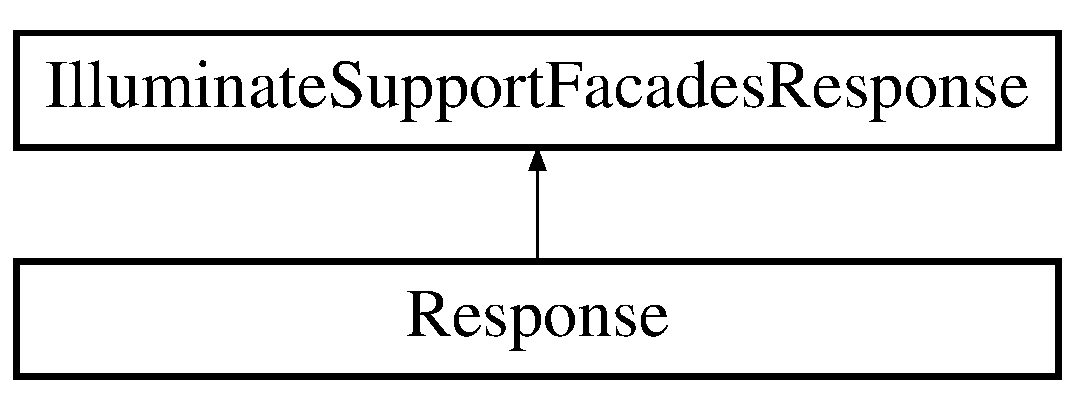
\includegraphics[height=2.000000cm]{class_illuminate_1_1_support_1_1_facades_1_1_response}
\end{center}
\end{figure}
\subsection*{Static Public Member Functions}
\begin{DoxyCompactItemize}
\item 
static \mbox{\hyperlink{class_illuminate_1_1_support_1_1_facades_1_1_response_ace4ab69686b08e356cd4305c9c4a5dbf}{make}} (\$content=\textquotesingle{}\textquotesingle{}, \$status=200, \$headers=array())
\item 
static \mbox{\hyperlink{class_illuminate_1_1_support_1_1_facades_1_1_response_a779627335e2e4bbb7858382cd706c00e}{view}} (\$view, \$data=array(), \$status=200, \$headers=array())
\item 
static \mbox{\hyperlink{class_illuminate_1_1_support_1_1_facades_1_1_response_a2ea308811b844bd1aa314083c14c8605}{json}} (\$data=array(), \$status=200, \$headers=array(), \$options=0)
\item 
static \mbox{\hyperlink{class_illuminate_1_1_support_1_1_facades_1_1_response_ae3af25f8ecea63cc6d2bbdb3b4faa656}{jsonp}} (\$callback, \$data=array(), \$status=200, \$headers=array(), \$options=0)
\item 
static \mbox{\hyperlink{class_illuminate_1_1_support_1_1_facades_1_1_response_aa2886263a826cf6d6481b5affc009656}{stream}} (\$callback, \$status=200, \$headers=array())
\item 
static \mbox{\hyperlink{class_illuminate_1_1_support_1_1_facades_1_1_response_a8496fd2c8b9553a89fde5d7b0faefce3}{download}} (\$\mbox{\hyperlink{class_illuminate_1_1_support_1_1_facades_1_1_response_a0791c3f7a4abd07bc240d6734d9ebbfe}{file}}, \$name=null, \$headers=array(), \$disposition=\textquotesingle{}attachment\textquotesingle{})
\item 
static \mbox{\hyperlink{class_illuminate_1_1_support_1_1_facades_1_1_response_a0791c3f7a4abd07bc240d6734d9ebbfe}{file}} (\$file, \$headers=array())
\item 
static \mbox{\hyperlink{class_illuminate_1_1_support_1_1_facades_1_1_response_a39a92b65c6598c8e72cf1c9dbad5cad1}{redirect\+To}} (\$path, \$status=302, \$headers=array(), \$secure=null)
\item 
static \mbox{\hyperlink{class_illuminate_1_1_support_1_1_facades_1_1_response_a3c4ceb412071ae0fe5d3fe1ce611a2db}{redirect\+To\+Route}} (\$route, \$parameters=array(), \$status=302, \$headers=array())
\item 
static \mbox{\hyperlink{class_illuminate_1_1_support_1_1_facades_1_1_response_af2811d5e6a939fbf613802bf656d9dd4}{redirect\+To\+Action}} (\$action, \$parameters=array(), \$status=302, \$headers=array())
\item 
static \mbox{\hyperlink{class_illuminate_1_1_support_1_1_facades_1_1_response_a73fcb2d662fbc4c5750385e548f7635d}{redirect\+Guest}} (\$path, \$status=302, \$headers=array(), \$secure=null)
\item 
static \mbox{\hyperlink{class_illuminate_1_1_support_1_1_facades_1_1_response_a75f7f05f8a855eac8f76bb0b93d7f6c0}{redirect\+To\+Intended}} (\$default=\textquotesingle{}/\textquotesingle{}, \$status=302, \$headers=array(), \$secure=null)
\item 
static \mbox{\hyperlink{class_illuminate_1_1_support_1_1_facades_1_1_response_ae12308120a0e244c64181a0111100568}{macro}} (\$name, \$macro)
\item 
static \mbox{\hyperlink{class_illuminate_1_1_support_1_1_facades_1_1_response_a6d0c18c89b5227e2e9ccf6a073a549ea}{mixin}} (\$mixin)
\item 
static \mbox{\hyperlink{class_illuminate_1_1_support_1_1_facades_1_1_response_a83ab61ed5befa2f787536443b466a7f2}{has\+Macro}} (\$name)
\end{DoxyCompactItemize}


\subsection{Member Function Documentation}
\mbox{\Hypertarget{class_illuminate_1_1_support_1_1_facades_1_1_response_a8496fd2c8b9553a89fde5d7b0faefce3}\label{class_illuminate_1_1_support_1_1_facades_1_1_response_a8496fd2c8b9553a89fde5d7b0faefce3}} 
\index{Illuminate\+::\+Support\+::\+Facades\+::\+Response@{Illuminate\+::\+Support\+::\+Facades\+::\+Response}!download@{download}}
\index{download@{download}!Illuminate\+::\+Support\+::\+Facades\+::\+Response@{Illuminate\+::\+Support\+::\+Facades\+::\+Response}}
\subsubsection{\texorpdfstring{download()}{download()}}
{\footnotesize\ttfamily static Illuminate\textbackslash{}\+Support\textbackslash{}\+Facades\textbackslash{}\+Response\+::download (\begin{DoxyParamCaption}\item[{}]{\$file,  }\item[{}]{\$name = {\ttfamily null},  }\item[{}]{\$headers = {\ttfamily array()},  }\item[{}]{\$disposition = {\ttfamily \textquotesingle{}attachment\textquotesingle{}} }\end{DoxyParamCaption})\hspace{0.3cm}{\ttfamily [static]}}

Create a new file download response.


\begin{DoxyParams}[1]{Parameters}
\textbackslash{}\+Spl\+File\+Info | string & {\em \$file} & \\
\hline
string & {\em \$name} & \\
\hline
array & {\em \$headers} & \\
\hline
string | null & {\em \$disposition} & \\
\hline
\end{DoxyParams}
\begin{DoxyReturn}{Returns}

\end{DoxyReturn}
\mbox{\Hypertarget{class_illuminate_1_1_support_1_1_facades_1_1_response_a0791c3f7a4abd07bc240d6734d9ebbfe}\label{class_illuminate_1_1_support_1_1_facades_1_1_response_a0791c3f7a4abd07bc240d6734d9ebbfe}} 
\index{Illuminate\+::\+Support\+::\+Facades\+::\+Response@{Illuminate\+::\+Support\+::\+Facades\+::\+Response}!file@{file}}
\index{file@{file}!Illuminate\+::\+Support\+::\+Facades\+::\+Response@{Illuminate\+::\+Support\+::\+Facades\+::\+Response}}
\subsubsection{\texorpdfstring{file()}{file()}}
{\footnotesize\ttfamily static Illuminate\textbackslash{}\+Support\textbackslash{}\+Facades\textbackslash{}\+Response\+::file (\begin{DoxyParamCaption}\item[{}]{\$file,  }\item[{}]{\$headers = {\ttfamily array()} }\end{DoxyParamCaption})\hspace{0.3cm}{\ttfamily [static]}}

Return the raw contents of a binary file.


\begin{DoxyParams}[1]{Parameters}
\textbackslash{}\+Spl\+File\+Info | string & {\em \$file} & \\
\hline
array & {\em \$headers} & \\
\hline
\end{DoxyParams}
\begin{DoxyReturn}{Returns}

\end{DoxyReturn}
\mbox{\Hypertarget{class_illuminate_1_1_support_1_1_facades_1_1_response_a83ab61ed5befa2f787536443b466a7f2}\label{class_illuminate_1_1_support_1_1_facades_1_1_response_a83ab61ed5befa2f787536443b466a7f2}} 
\index{Illuminate\+::\+Support\+::\+Facades\+::\+Response@{Illuminate\+::\+Support\+::\+Facades\+::\+Response}!has\+Macro@{has\+Macro}}
\index{has\+Macro@{has\+Macro}!Illuminate\+::\+Support\+::\+Facades\+::\+Response@{Illuminate\+::\+Support\+::\+Facades\+::\+Response}}
\subsubsection{\texorpdfstring{has\+Macro()}{hasMacro()}}
{\footnotesize\ttfamily static Illuminate\textbackslash{}\+Support\textbackslash{}\+Facades\textbackslash{}\+Response\+::has\+Macro (\begin{DoxyParamCaption}\item[{}]{\$name }\end{DoxyParamCaption})\hspace{0.3cm}{\ttfamily [static]}}

Checks if macro is registered.


\begin{DoxyParams}[1]{Parameters}
string & {\em \$name} & \\
\hline
\end{DoxyParams}
\begin{DoxyReturn}{Returns}
bool 
\end{DoxyReturn}
\mbox{\Hypertarget{class_illuminate_1_1_support_1_1_facades_1_1_response_a2ea308811b844bd1aa314083c14c8605}\label{class_illuminate_1_1_support_1_1_facades_1_1_response_a2ea308811b844bd1aa314083c14c8605}} 
\index{Illuminate\+::\+Support\+::\+Facades\+::\+Response@{Illuminate\+::\+Support\+::\+Facades\+::\+Response}!json@{json}}
\index{json@{json}!Illuminate\+::\+Support\+::\+Facades\+::\+Response@{Illuminate\+::\+Support\+::\+Facades\+::\+Response}}
\subsubsection{\texorpdfstring{json()}{json()}}
{\footnotesize\ttfamily static Illuminate\textbackslash{}\+Support\textbackslash{}\+Facades\textbackslash{}\+Response\+::json (\begin{DoxyParamCaption}\item[{}]{\$data = {\ttfamily array()},  }\item[{}]{\$status = {\ttfamily 200},  }\item[{}]{\$headers = {\ttfamily array()},  }\item[{}]{\$options = {\ttfamily 0} }\end{DoxyParamCaption})\hspace{0.3cm}{\ttfamily [static]}}

Return a new J\+S\+ON response from the application.


\begin{DoxyParams}[1]{Parameters}
mixed & {\em \$data} & \\
\hline
int & {\em \$status} & \\
\hline
array & {\em \$headers} & \\
\hline
int & {\em \$options} & \\
\hline
\end{DoxyParams}
\begin{DoxyReturn}{Returns}

\end{DoxyReturn}
\mbox{\Hypertarget{class_illuminate_1_1_support_1_1_facades_1_1_response_ae3af25f8ecea63cc6d2bbdb3b4faa656}\label{class_illuminate_1_1_support_1_1_facades_1_1_response_ae3af25f8ecea63cc6d2bbdb3b4faa656}} 
\index{Illuminate\+::\+Support\+::\+Facades\+::\+Response@{Illuminate\+::\+Support\+::\+Facades\+::\+Response}!jsonp@{jsonp}}
\index{jsonp@{jsonp}!Illuminate\+::\+Support\+::\+Facades\+::\+Response@{Illuminate\+::\+Support\+::\+Facades\+::\+Response}}
\subsubsection{\texorpdfstring{jsonp()}{jsonp()}}
{\footnotesize\ttfamily static Illuminate\textbackslash{}\+Support\textbackslash{}\+Facades\textbackslash{}\+Response\+::jsonp (\begin{DoxyParamCaption}\item[{}]{\$callback,  }\item[{}]{\$data = {\ttfamily array()},  }\item[{}]{\$status = {\ttfamily 200},  }\item[{}]{\$headers = {\ttfamily array()},  }\item[{}]{\$options = {\ttfamily 0} }\end{DoxyParamCaption})\hspace{0.3cm}{\ttfamily [static]}}

Return a new J\+S\+O\+NP response from the application.


\begin{DoxyParams}[1]{Parameters}
string & {\em \$callback} & \\
\hline
mixed & {\em \$data} & \\
\hline
int & {\em \$status} & \\
\hline
array & {\em \$headers} & \\
\hline
int & {\em \$options} & \\
\hline
\end{DoxyParams}
\begin{DoxyReturn}{Returns}

\end{DoxyReturn}
\mbox{\Hypertarget{class_illuminate_1_1_support_1_1_facades_1_1_response_ae12308120a0e244c64181a0111100568}\label{class_illuminate_1_1_support_1_1_facades_1_1_response_ae12308120a0e244c64181a0111100568}} 
\index{Illuminate\+::\+Support\+::\+Facades\+::\+Response@{Illuminate\+::\+Support\+::\+Facades\+::\+Response}!macro@{macro}}
\index{macro@{macro}!Illuminate\+::\+Support\+::\+Facades\+::\+Response@{Illuminate\+::\+Support\+::\+Facades\+::\+Response}}
\subsubsection{\texorpdfstring{macro()}{macro()}}
{\footnotesize\ttfamily static Illuminate\textbackslash{}\+Support\textbackslash{}\+Facades\textbackslash{}\+Response\+::macro (\begin{DoxyParamCaption}\item[{}]{\$name,  }\item[{}]{\$macro }\end{DoxyParamCaption})\hspace{0.3cm}{\ttfamily [static]}}

Register a custom macro.


\begin{DoxyParams}[1]{Parameters}
string & {\em \$name} & \\
\hline
object | callable & {\em \$macro} & \\
\hline
\end{DoxyParams}
\begin{DoxyReturn}{Returns}
void 
\end{DoxyReturn}
\mbox{\Hypertarget{class_illuminate_1_1_support_1_1_facades_1_1_response_ace4ab69686b08e356cd4305c9c4a5dbf}\label{class_illuminate_1_1_support_1_1_facades_1_1_response_ace4ab69686b08e356cd4305c9c4a5dbf}} 
\index{Illuminate\+::\+Support\+::\+Facades\+::\+Response@{Illuminate\+::\+Support\+::\+Facades\+::\+Response}!make@{make}}
\index{make@{make}!Illuminate\+::\+Support\+::\+Facades\+::\+Response@{Illuminate\+::\+Support\+::\+Facades\+::\+Response}}
\subsubsection{\texorpdfstring{make()}{make()}}
{\footnotesize\ttfamily static Illuminate\textbackslash{}\+Support\textbackslash{}\+Facades\textbackslash{}\+Response\+::make (\begin{DoxyParamCaption}\item[{}]{\$content = {\ttfamily \textquotesingle{}\textquotesingle{}},  }\item[{}]{\$status = {\ttfamily 200},  }\item[{}]{\$headers = {\ttfamily array()} }\end{DoxyParamCaption})\hspace{0.3cm}{\ttfamily [static]}}

Return a new response from the application.


\begin{DoxyParams}[1]{Parameters}
string & {\em \$content} & \\
\hline
int & {\em \$status} & \\
\hline
array & {\em \$headers} & \\
\hline
\end{DoxyParams}
\begin{DoxyReturn}{Returns}

\end{DoxyReturn}
\mbox{\Hypertarget{class_illuminate_1_1_support_1_1_facades_1_1_response_a6d0c18c89b5227e2e9ccf6a073a549ea}\label{class_illuminate_1_1_support_1_1_facades_1_1_response_a6d0c18c89b5227e2e9ccf6a073a549ea}} 
\index{Illuminate\+::\+Support\+::\+Facades\+::\+Response@{Illuminate\+::\+Support\+::\+Facades\+::\+Response}!mixin@{mixin}}
\index{mixin@{mixin}!Illuminate\+::\+Support\+::\+Facades\+::\+Response@{Illuminate\+::\+Support\+::\+Facades\+::\+Response}}
\subsubsection{\texorpdfstring{mixin()}{mixin()}}
{\footnotesize\ttfamily static Illuminate\textbackslash{}\+Support\textbackslash{}\+Facades\textbackslash{}\+Response\+::mixin (\begin{DoxyParamCaption}\item[{}]{\$mixin }\end{DoxyParamCaption})\hspace{0.3cm}{\ttfamily [static]}}

Mix another object into the class.


\begin{DoxyParams}[1]{Parameters}
object & {\em \$mixin} & \\
\hline
\end{DoxyParams}
\begin{DoxyReturn}{Returns}
void 
\end{DoxyReturn}
\mbox{\Hypertarget{class_illuminate_1_1_support_1_1_facades_1_1_response_a73fcb2d662fbc4c5750385e548f7635d}\label{class_illuminate_1_1_support_1_1_facades_1_1_response_a73fcb2d662fbc4c5750385e548f7635d}} 
\index{Illuminate\+::\+Support\+::\+Facades\+::\+Response@{Illuminate\+::\+Support\+::\+Facades\+::\+Response}!redirect\+Guest@{redirect\+Guest}}
\index{redirect\+Guest@{redirect\+Guest}!Illuminate\+::\+Support\+::\+Facades\+::\+Response@{Illuminate\+::\+Support\+::\+Facades\+::\+Response}}
\subsubsection{\texorpdfstring{redirect\+Guest()}{redirectGuest()}}
{\footnotesize\ttfamily static Illuminate\textbackslash{}\+Support\textbackslash{}\+Facades\textbackslash{}\+Response\+::redirect\+Guest (\begin{DoxyParamCaption}\item[{}]{\$path,  }\item[{}]{\$status = {\ttfamily 302},  }\item[{}]{\$headers = {\ttfamily array()},  }\item[{}]{\$secure = {\ttfamily null} }\end{DoxyParamCaption})\hspace{0.3cm}{\ttfamily [static]}}

Create a new redirect response, while putting the current \mbox{\hyperlink{class_illuminate_1_1_support_1_1_facades_1_1_u_r_l}{U\+RL}} in the session.


\begin{DoxyParams}[1]{Parameters}
string & {\em \$path} & \\
\hline
int & {\em \$status} & \\
\hline
array & {\em \$headers} & \\
\hline
bool | null & {\em \$secure} & \\
\hline
\end{DoxyParams}
\begin{DoxyReturn}{Returns}

\end{DoxyReturn}
\mbox{\Hypertarget{class_illuminate_1_1_support_1_1_facades_1_1_response_a39a92b65c6598c8e72cf1c9dbad5cad1}\label{class_illuminate_1_1_support_1_1_facades_1_1_response_a39a92b65c6598c8e72cf1c9dbad5cad1}} 
\index{Illuminate\+::\+Support\+::\+Facades\+::\+Response@{Illuminate\+::\+Support\+::\+Facades\+::\+Response}!redirect\+To@{redirect\+To}}
\index{redirect\+To@{redirect\+To}!Illuminate\+::\+Support\+::\+Facades\+::\+Response@{Illuminate\+::\+Support\+::\+Facades\+::\+Response}}
\subsubsection{\texorpdfstring{redirect\+To()}{redirectTo()}}
{\footnotesize\ttfamily static Illuminate\textbackslash{}\+Support\textbackslash{}\+Facades\textbackslash{}\+Response\+::redirect\+To (\begin{DoxyParamCaption}\item[{}]{\$path,  }\item[{}]{\$status = {\ttfamily 302},  }\item[{}]{\$headers = {\ttfamily array()},  }\item[{}]{\$secure = {\ttfamily null} }\end{DoxyParamCaption})\hspace{0.3cm}{\ttfamily [static]}}

Create a new redirect response to the given path.


\begin{DoxyParams}[1]{Parameters}
string & {\em \$path} & \\
\hline
int & {\em \$status} & \\
\hline
array & {\em \$headers} & \\
\hline
bool | null & {\em \$secure} & \\
\hline
\end{DoxyParams}
\begin{DoxyReturn}{Returns}

\end{DoxyReturn}
\mbox{\Hypertarget{class_illuminate_1_1_support_1_1_facades_1_1_response_af2811d5e6a939fbf613802bf656d9dd4}\label{class_illuminate_1_1_support_1_1_facades_1_1_response_af2811d5e6a939fbf613802bf656d9dd4}} 
\index{Illuminate\+::\+Support\+::\+Facades\+::\+Response@{Illuminate\+::\+Support\+::\+Facades\+::\+Response}!redirect\+To\+Action@{redirect\+To\+Action}}
\index{redirect\+To\+Action@{redirect\+To\+Action}!Illuminate\+::\+Support\+::\+Facades\+::\+Response@{Illuminate\+::\+Support\+::\+Facades\+::\+Response}}
\subsubsection{\texorpdfstring{redirect\+To\+Action()}{redirectToAction()}}
{\footnotesize\ttfamily static Illuminate\textbackslash{}\+Support\textbackslash{}\+Facades\textbackslash{}\+Response\+::redirect\+To\+Action (\begin{DoxyParamCaption}\item[{}]{\$action,  }\item[{}]{\$parameters = {\ttfamily array()},  }\item[{}]{\$status = {\ttfamily 302},  }\item[{}]{\$headers = {\ttfamily array()} }\end{DoxyParamCaption})\hspace{0.3cm}{\ttfamily [static]}}

Create a new redirect response to a controller action.


\begin{DoxyParams}[1]{Parameters}
string & {\em \$action} & \\
\hline
array & {\em \$parameters} & \\
\hline
int & {\em \$status} & \\
\hline
array & {\em \$headers} & \\
\hline
\end{DoxyParams}
\begin{DoxyReturn}{Returns}

\end{DoxyReturn}
\mbox{\Hypertarget{class_illuminate_1_1_support_1_1_facades_1_1_response_a75f7f05f8a855eac8f76bb0b93d7f6c0}\label{class_illuminate_1_1_support_1_1_facades_1_1_response_a75f7f05f8a855eac8f76bb0b93d7f6c0}} 
\index{Illuminate\+::\+Support\+::\+Facades\+::\+Response@{Illuminate\+::\+Support\+::\+Facades\+::\+Response}!redirect\+To\+Intended@{redirect\+To\+Intended}}
\index{redirect\+To\+Intended@{redirect\+To\+Intended}!Illuminate\+::\+Support\+::\+Facades\+::\+Response@{Illuminate\+::\+Support\+::\+Facades\+::\+Response}}
\subsubsection{\texorpdfstring{redirect\+To\+Intended()}{redirectToIntended()}}
{\footnotesize\ttfamily static Illuminate\textbackslash{}\+Support\textbackslash{}\+Facades\textbackslash{}\+Response\+::redirect\+To\+Intended (\begin{DoxyParamCaption}\item[{}]{\$default = {\ttfamily \textquotesingle{}/\textquotesingle{}},  }\item[{}]{\$status = {\ttfamily 302},  }\item[{}]{\$headers = {\ttfamily array()},  }\item[{}]{\$secure = {\ttfamily null} }\end{DoxyParamCaption})\hspace{0.3cm}{\ttfamily [static]}}

Create a new redirect response to the previously intended location.


\begin{DoxyParams}[1]{Parameters}
string & {\em \$default} & \\
\hline
int & {\em \$status} & \\
\hline
array & {\em \$headers} & \\
\hline
bool | null & {\em \$secure} & \\
\hline
\end{DoxyParams}
\begin{DoxyReturn}{Returns}

\end{DoxyReturn}
\mbox{\Hypertarget{class_illuminate_1_1_support_1_1_facades_1_1_response_a3c4ceb412071ae0fe5d3fe1ce611a2db}\label{class_illuminate_1_1_support_1_1_facades_1_1_response_a3c4ceb412071ae0fe5d3fe1ce611a2db}} 
\index{Illuminate\+::\+Support\+::\+Facades\+::\+Response@{Illuminate\+::\+Support\+::\+Facades\+::\+Response}!redirect\+To\+Route@{redirect\+To\+Route}}
\index{redirect\+To\+Route@{redirect\+To\+Route}!Illuminate\+::\+Support\+::\+Facades\+::\+Response@{Illuminate\+::\+Support\+::\+Facades\+::\+Response}}
\subsubsection{\texorpdfstring{redirect\+To\+Route()}{redirectToRoute()}}
{\footnotesize\ttfamily static Illuminate\textbackslash{}\+Support\textbackslash{}\+Facades\textbackslash{}\+Response\+::redirect\+To\+Route (\begin{DoxyParamCaption}\item[{}]{\$route,  }\item[{}]{\$parameters = {\ttfamily array()},  }\item[{}]{\$status = {\ttfamily 302},  }\item[{}]{\$headers = {\ttfamily array()} }\end{DoxyParamCaption})\hspace{0.3cm}{\ttfamily [static]}}

Create a new redirect response to a named route.


\begin{DoxyParams}[1]{Parameters}
string & {\em \$route} & \\
\hline
array & {\em \$parameters} & \\
\hline
int & {\em \$status} & \\
\hline
array & {\em \$headers} & \\
\hline
\end{DoxyParams}
\begin{DoxyReturn}{Returns}

\end{DoxyReturn}
\mbox{\Hypertarget{class_illuminate_1_1_support_1_1_facades_1_1_response_aa2886263a826cf6d6481b5affc009656}\label{class_illuminate_1_1_support_1_1_facades_1_1_response_aa2886263a826cf6d6481b5affc009656}} 
\index{Illuminate\+::\+Support\+::\+Facades\+::\+Response@{Illuminate\+::\+Support\+::\+Facades\+::\+Response}!stream@{stream}}
\index{stream@{stream}!Illuminate\+::\+Support\+::\+Facades\+::\+Response@{Illuminate\+::\+Support\+::\+Facades\+::\+Response}}
\subsubsection{\texorpdfstring{stream()}{stream()}}
{\footnotesize\ttfamily static Illuminate\textbackslash{}\+Support\textbackslash{}\+Facades\textbackslash{}\+Response\+::stream (\begin{DoxyParamCaption}\item[{}]{\$callback,  }\item[{}]{\$status = {\ttfamily 200},  }\item[{}]{\$headers = {\ttfamily array()} }\end{DoxyParamCaption})\hspace{0.3cm}{\ttfamily [static]}}

Return a new streamed response from the application.


\begin{DoxyParams}[1]{Parameters}
\textbackslash{}\+Closure & {\em \$callback} & \\
\hline
int & {\em \$status} & \\
\hline
array & {\em \$headers} & \\
\hline
\end{DoxyParams}
\begin{DoxyReturn}{Returns}

\end{DoxyReturn}
\mbox{\Hypertarget{class_illuminate_1_1_support_1_1_facades_1_1_response_a779627335e2e4bbb7858382cd706c00e}\label{class_illuminate_1_1_support_1_1_facades_1_1_response_a779627335e2e4bbb7858382cd706c00e}} 
\index{Illuminate\+::\+Support\+::\+Facades\+::\+Response@{Illuminate\+::\+Support\+::\+Facades\+::\+Response}!view@{view}}
\index{view@{view}!Illuminate\+::\+Support\+::\+Facades\+::\+Response@{Illuminate\+::\+Support\+::\+Facades\+::\+Response}}
\subsubsection{\texorpdfstring{view()}{view()}}
{\footnotesize\ttfamily static Illuminate\textbackslash{}\+Support\textbackslash{}\+Facades\textbackslash{}\+Response\+::view (\begin{DoxyParamCaption}\item[{}]{\$view,  }\item[{}]{\$data = {\ttfamily array()},  }\item[{}]{\$status = {\ttfamily 200},  }\item[{}]{\$headers = {\ttfamily array()} }\end{DoxyParamCaption})\hspace{0.3cm}{\ttfamily [static]}}

Return a new view response from the application.


\begin{DoxyParams}[1]{Parameters}
string & {\em \$view} & \\
\hline
array & {\em \$data} & \\
\hline
int & {\em \$status} & \\
\hline
array & {\em \$headers} & \\
\hline
\end{DoxyParams}
\begin{DoxyReturn}{Returns}

\end{DoxyReturn}


The documentation for this class was generated from the following file\+:\begin{DoxyCompactItemize}
\item 
\+\_\+ide\+\_\+helper.\+php\end{DoxyCompactItemize}

\hypertarget{class_response}{}\section{Response Class Reference}
\label{class_response}\index{Response@{Response}}
Inheritance diagram for Response\+:\begin{figure}[H]
\begin{center}
\leavevmode
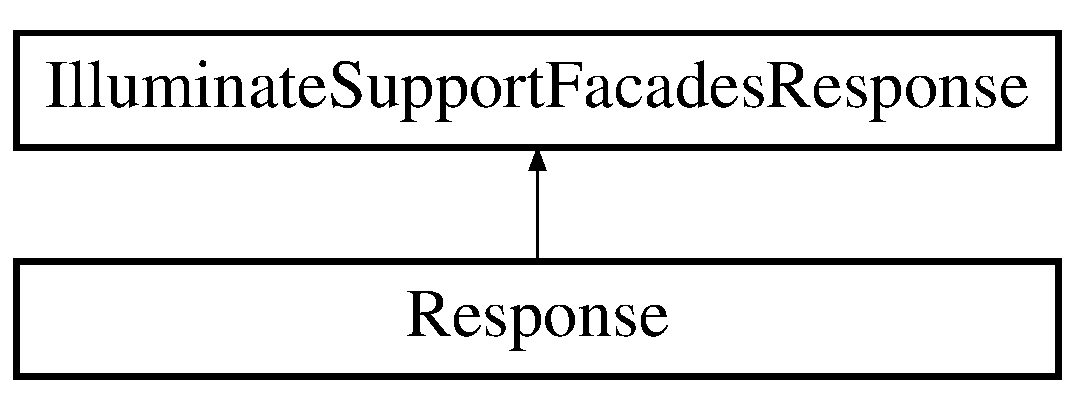
\includegraphics[height=2.000000cm]{class_response}
\end{center}
\end{figure}
\subsection*{Additional Inherited Members}


The documentation for this class was generated from the following file\+:\begin{DoxyCompactItemize}
\item 
\+\_\+ide\+\_\+helper.\+php\end{DoxyCompactItemize}

\hypertarget{class_illuminate_1_1_support_1_1_facades_1_1_route}{}\section{Illuminate\textbackslash{}Support\textbackslash{}Facades\textbackslash{}Route Class Reference}
\label{class_illuminate_1_1_support_1_1_facades_1_1_route}\index{Illuminate\textbackslash{}\+Support\textbackslash{}\+Facades\textbackslash{}\+Route@{Illuminate\textbackslash{}\+Support\textbackslash{}\+Facades\textbackslash{}\+Route}}
Inheritance diagram for Illuminate\textbackslash{}Support\textbackslash{}Facades\textbackslash{}Route\+:\begin{figure}[H]
\begin{center}
\leavevmode
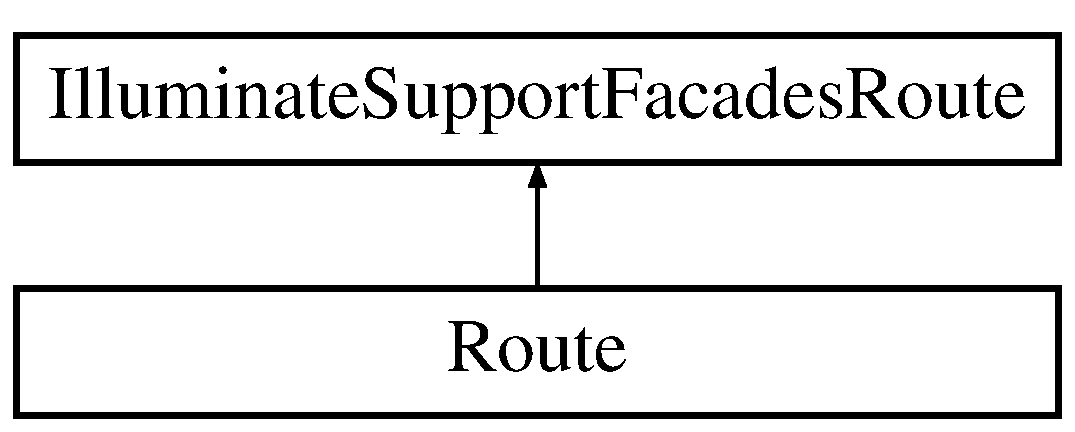
\includegraphics[height=2.000000cm]{class_illuminate_1_1_support_1_1_facades_1_1_route}
\end{center}
\end{figure}
\subsection*{Static Public Member Functions}
\begin{DoxyCompactItemize}
\item 
static \mbox{\hyperlink{class_illuminate_1_1_support_1_1_facades_1_1_route_a39cd5af406f569f04257beadad32f22a}{get}} (\$uri, \$action=null)
\item 
static \mbox{\hyperlink{class_illuminate_1_1_support_1_1_facades_1_1_route_a3e87a5845aaa31e93fcf49f6c3bb9c0f}{post}} (\$uri, \$action=null)
\item 
static \mbox{\hyperlink{class_illuminate_1_1_support_1_1_facades_1_1_route_ac147418c43c1fde624c9e9ee3a8b97e0}{put}} (\$uri, \$action=null)
\item 
static \mbox{\hyperlink{class_illuminate_1_1_support_1_1_facades_1_1_route_a07351975af02a62cda512488b3057038}{patch}} (\$uri, \$action=null)
\item 
static \mbox{\hyperlink{class_illuminate_1_1_support_1_1_facades_1_1_route_a9d7c9d2fb6b52af124f3d0d354048649}{delete}} (\$uri, \$action=null)
\item 
static \mbox{\hyperlink{class_illuminate_1_1_support_1_1_facades_1_1_route_a56299381f0cc42d0701d1149d6923d6d}{options}} (\$uri, \$action=null)
\item 
static \mbox{\hyperlink{class_illuminate_1_1_support_1_1_facades_1_1_route_acd44678d4fb5ef17bad21a70795df5f1}{any}} (\$uri, \$action=null)
\item 
static \mbox{\hyperlink{class_illuminate_1_1_support_1_1_facades_1_1_route_a3f0681b90b6ff2207c419498712a7ba4}{fallback}} (\$action)
\item 
static \mbox{\hyperlink{class_illuminate_1_1_support_1_1_facades_1_1_route_aabe01372a09b36ba51904a73c2ffa526}{redirect}} (\$uri, \$destination, \$status=301)
\item 
static \mbox{\hyperlink{class_illuminate_1_1_support_1_1_facades_1_1_route_a0ad562188e1e8adef7e084599b20fcf3}{view}} (\$uri, \$view, \$data=array())
\item 
static \mbox{\hyperlink{class_illuminate_1_1_support_1_1_facades_1_1_route_a883b4c2ff585ed08b6543af097a9fee0}{match}} (\$methods, \$uri, \$action=null)
\item 
static \mbox{\hyperlink{class_illuminate_1_1_support_1_1_facades_1_1_route_a474685a13bb6afbb588369b5abae1885}{resources}} (\$resources)
\item 
static \mbox{\hyperlink{class_illuminate_1_1_support_1_1_facades_1_1_route_a43f06987528f8a3f90ddb29395d93bd0}{resource}} (\$name, \$controller, \$\mbox{\hyperlink{class_illuminate_1_1_support_1_1_facades_1_1_route_a56299381f0cc42d0701d1149d6923d6d}{options}}=array())
\item 
static \mbox{\hyperlink{class_illuminate_1_1_support_1_1_facades_1_1_route_a870a8af5be97776cb08cd19e7681665b}{api\+Resource}} (\$name, \$controller, \$\mbox{\hyperlink{class_illuminate_1_1_support_1_1_facades_1_1_route_a56299381f0cc42d0701d1149d6923d6d}{options}}=array())
\item 
static \mbox{\hyperlink{class_illuminate_1_1_support_1_1_facades_1_1_route_ac33b88549eeaaed8325ee4b479a8c132}{group}} (\$attributes, \$routes)
\item 
static \mbox{\hyperlink{class_illuminate_1_1_support_1_1_facades_1_1_route_a8593864cb4512c462ea6fe2135f97490}{merge\+With\+Last\+Group}} (\$new)
\item 
static \mbox{\hyperlink{class_illuminate_1_1_support_1_1_facades_1_1_route_ac204f4635943e403474495a26cb4cfb6}{get\+Last\+Group\+Prefix}} ()
\item 
static \mbox{\hyperlink{class_illuminate_1_1_support_1_1_facades_1_1_route_ac0573684cafafad11cb8fe7c470a766b}{respond\+With\+Route}} (\$name)
\item 
static \mbox{\hyperlink{class_illuminate_1_1_support_1_1_facades_1_1_route_a861f30796a663e1d1e8982bc7ff9a8b8}{dispatch}} (\$request)
\item 
static \mbox{\hyperlink{class_illuminate_1_1_support_1_1_facades_1_1_route_a22e9a656dbe34e0311a566c90330a3a6}{dispatch\+To\+Route}} (\$request)
\item 
static \mbox{\hyperlink{class_illuminate_1_1_support_1_1_facades_1_1_route_ad8d94099c533eb3f93a4fa0884e69716}{gather\+Route\+Middleware}} (\$route)
\item 
static \mbox{\hyperlink{class_illuminate_1_1_support_1_1_facades_1_1_route_adf6831262c25fa426d81fec205559bcd}{prepare\+Response}} (\$request, \$response)
\item 
static \mbox{\hyperlink{class_illuminate_1_1_support_1_1_facades_1_1_route_a93f7f1fd6665fa39d529aa12ccbec22e}{to\+Response}} (\$request, \$response)
\item 
static \mbox{\hyperlink{class_illuminate_1_1_support_1_1_facades_1_1_route_a5a2a3e65c09e2e548773a5513ae4e9f9}{substitute\+Bindings}} (\$route)
\item 
static \mbox{\hyperlink{class_illuminate_1_1_support_1_1_facades_1_1_route_a8b47baf3e67a44458d5359a653250714}{substitute\+Implicit\+Bindings}} (\$route)
\item 
static \mbox{\hyperlink{class_illuminate_1_1_support_1_1_facades_1_1_route_a5a3bc3b67390be84a837c090d97f8993}{matched}} (\$callback)
\item 
static \mbox{\hyperlink{class_illuminate_1_1_support_1_1_facades_1_1_route_ac8cd393a47c3e27405e140e0b143aec8}{get\+Middleware}} ()
\item 
static \mbox{\hyperlink{class_illuminate_1_1_support_1_1_facades_1_1_route_a2303469c734df3248247dc66ec3e6b4f}{alias\+Middleware}} (\$name, \$class)
\item 
static \mbox{\hyperlink{class_illuminate_1_1_support_1_1_facades_1_1_route_abf3af941c9614b377ce6d798aaa671a6}{has\+Middleware\+Group}} (\$name)
\item 
static \mbox{\hyperlink{class_illuminate_1_1_support_1_1_facades_1_1_route_a8124e67845527e8c6550543b9859561f}{get\+Middleware\+Groups}} ()
\item 
static \mbox{\hyperlink{class_illuminate_1_1_support_1_1_facades_1_1_route_adc46eb120062bf3a3488ed866b868a63}{middleware\+Group}} (\$name, \$middleware)
\item 
static \mbox{\hyperlink{class_illuminate_1_1_support_1_1_facades_1_1_route_a18c9e3d1b6ee2af7b94f2aa2265c0c5c}{prepend\+Middleware\+To\+Group}} (\$\mbox{\hyperlink{class_illuminate_1_1_support_1_1_facades_1_1_route_ac33b88549eeaaed8325ee4b479a8c132}{group}}, \$middleware)
\item 
static \mbox{\hyperlink{class_illuminate_1_1_support_1_1_facades_1_1_route_a5ed4aa5fc4f06f149321abd0671f2176}{push\+Middleware\+To\+Group}} (\$\mbox{\hyperlink{class_illuminate_1_1_support_1_1_facades_1_1_route_ac33b88549eeaaed8325ee4b479a8c132}{group}}, \$middleware)
\item 
static \mbox{\hyperlink{class_illuminate_1_1_support_1_1_facades_1_1_route_aa8f9b61452dcd905b61494ea174d4956}{bind}} (\$key, \$binder)
\item 
static \mbox{\hyperlink{class_illuminate_1_1_support_1_1_facades_1_1_route_ac98c5b1745935107addfb0fc224a696f}{model}} (\$key, \$class, \$callback=null)
\item 
static \mbox{\hyperlink{class_illuminate_1_1_support_1_1_facades_1_1_route_aa5e004b320250adff27b176fdc14f775}{get\+Binding\+Callback}} (\$key)
\item 
static \mbox{\hyperlink{class_illuminate_1_1_support_1_1_facades_1_1_route_a937714eb57fd5cdc4763873eb8f28e45}{get\+Patterns}} ()
\item 
static \mbox{\hyperlink{class_illuminate_1_1_support_1_1_facades_1_1_route_a8f488e142dfe7fb74ee7d07876627d98}{pattern}} (\$key, \$pattern)
\item 
static \mbox{\hyperlink{class_illuminate_1_1_support_1_1_facades_1_1_route_a5ffa318d86f489c77ed7e2ce757e0cd3}{patterns}} (\$patterns)
\item 
static \mbox{\hyperlink{class_illuminate_1_1_support_1_1_facades_1_1_route_a79a54acb58c2839bd713b9837fb7df4a}{has\+Group\+Stack}} ()
\item 
static \mbox{\hyperlink{class_illuminate_1_1_support_1_1_facades_1_1_route_a82530084fbf4f15035b837ad7f76c885}{get\+Group\+Stack}} ()
\item 
static \mbox{\hyperlink{class_illuminate_1_1_support_1_1_facades_1_1_route_ab0ac1edc61bd2c5428d0470857d257b5}{input}} (\$key, \$default=null)
\item 
static \mbox{\hyperlink{class_illuminate_1_1_support_1_1_facades_1_1_route_a2d374f929804e9019f0edbff3b6114b0}{get\+Current\+Request}} ()
\item 
static \mbox{\hyperlink{class_illuminate_1_1_support_1_1_facades_1_1_route_a45a22de35b188f7aecb60ea655a6b4ae}{get\+Current\+Route}} ()
\item 
static \mbox{\hyperlink{class_illuminate_1_1_support_1_1_facades_1_1_route_aeec1a8e61c2cc8b2c74a809b696f068d}{current}} ()
\item 
static \mbox{\hyperlink{class_illuminate_1_1_support_1_1_facades_1_1_route_ab8e83d61a5fa5f28ca782e540d4cb65b}{has}} (\$name)
\item 
static \mbox{\hyperlink{class_illuminate_1_1_support_1_1_facades_1_1_route_aa51df157f19235dfa43fe5411466c559}{current\+Route\+Name}} ()
\item 
static \mbox{\hyperlink{class_illuminate_1_1_support_1_1_facades_1_1_route_a9b5244a7e5f3c63d5793da62a58ba646}{is}} (\$\mbox{\hyperlink{class_illuminate_1_1_support_1_1_facades_1_1_route_a5ffa318d86f489c77ed7e2ce757e0cd3}{patterns}}=null)
\item 
static \mbox{\hyperlink{class_illuminate_1_1_support_1_1_facades_1_1_route_a6a94528e537e7c79630ee8093c46ef28}{current\+Route\+Named}} (\$\mbox{\hyperlink{class_illuminate_1_1_support_1_1_facades_1_1_route_a5ffa318d86f489c77ed7e2ce757e0cd3}{patterns}}=null)
\item 
static \mbox{\hyperlink{class_illuminate_1_1_support_1_1_facades_1_1_route_a6ccd7018141278ca72001186a2c60444}{current\+Route\+Action}} ()
\item 
static \mbox{\hyperlink{class_illuminate_1_1_support_1_1_facades_1_1_route_adfbb616bc0fb81bd33b68ea7080444fb}{uses}} (\$\mbox{\hyperlink{class_illuminate_1_1_support_1_1_facades_1_1_route_a5ffa318d86f489c77ed7e2ce757e0cd3}{patterns}}=null)
\item 
static \mbox{\hyperlink{class_illuminate_1_1_support_1_1_facades_1_1_route_add49710873dc072055a44e6e78a20eb7}{current\+Route\+Uses}} (\$action)
\item 
static \mbox{\hyperlink{class_illuminate_1_1_support_1_1_facades_1_1_route_ad277eb6383efcee9dcd3ea564b39ad0f}{auth}} ()
\item 
static \mbox{\hyperlink{class_illuminate_1_1_support_1_1_facades_1_1_route_a109da236bab9351cc8a449917b32abb7}{singular\+Resource\+Parameters}} (\$singular=true)
\item 
static \mbox{\hyperlink{class_illuminate_1_1_support_1_1_facades_1_1_route_a99d41dab6379da413243e2b22c4cb336}{resource\+Parameters}} (\$parameters=array())
\item 
static \mbox{\hyperlink{class_illuminate_1_1_support_1_1_facades_1_1_route_a7e9d53bbab3ce3e9711d0eeb9643dc32}{resource\+Verbs}} (\$verbs=array())
\item 
static \mbox{\hyperlink{class_illuminate_1_1_support_1_1_facades_1_1_route_a8d907c259d15756737cb208e4acbd8a7}{get\+Routes}} ()
\item 
static \mbox{\hyperlink{class_illuminate_1_1_support_1_1_facades_1_1_route_a1622d20eba5c59f93b6d28a021439769}{set\+Routes}} (\$routes)
\item 
static \mbox{\hyperlink{class_illuminate_1_1_support_1_1_facades_1_1_route_aac6eba2155e061b8cff3a6c073ba9b86}{macro}} (\$name, \$macro)
\item 
static \mbox{\hyperlink{class_illuminate_1_1_support_1_1_facades_1_1_route_a2c2a3b5d21f7154bf5f028fc578cb834}{mixin}} (\$mixin)
\item 
static \mbox{\hyperlink{class_illuminate_1_1_support_1_1_facades_1_1_route_a57b330e021063745532d1790f82f60fc}{has\+Macro}} (\$name)
\item 
static \mbox{\hyperlink{class_illuminate_1_1_support_1_1_facades_1_1_route_a5d946c1e8f872ba226464d40ffb1bdb9}{macro\+Call}} (\$method, \$parameters)
\end{DoxyCompactItemize}


\subsection{Member Function Documentation}
\mbox{\Hypertarget{class_illuminate_1_1_support_1_1_facades_1_1_route_a2303469c734df3248247dc66ec3e6b4f}\label{class_illuminate_1_1_support_1_1_facades_1_1_route_a2303469c734df3248247dc66ec3e6b4f}} 
\index{Illuminate\+::\+Support\+::\+Facades\+::\+Route@{Illuminate\+::\+Support\+::\+Facades\+::\+Route}!alias\+Middleware@{alias\+Middleware}}
\index{alias\+Middleware@{alias\+Middleware}!Illuminate\+::\+Support\+::\+Facades\+::\+Route@{Illuminate\+::\+Support\+::\+Facades\+::\+Route}}
\subsubsection{\texorpdfstring{alias\+Middleware()}{aliasMiddleware()}}
{\footnotesize\ttfamily static Illuminate\textbackslash{}\+Support\textbackslash{}\+Facades\textbackslash{}\+Route\+::alias\+Middleware (\begin{DoxyParamCaption}\item[{}]{\$name,  }\item[{}]{\$class }\end{DoxyParamCaption})\hspace{0.3cm}{\ttfamily [static]}}

Register a short-\/hand name for a middleware.


\begin{DoxyParams}[1]{Parameters}
string & {\em \$name} & \\
\hline
string & {\em \$class} & \\
\hline
\end{DoxyParams}
\begin{DoxyReturn}{Returns}
\$this 
\end{DoxyReturn}
\mbox{\Hypertarget{class_illuminate_1_1_support_1_1_facades_1_1_route_acd44678d4fb5ef17bad21a70795df5f1}\label{class_illuminate_1_1_support_1_1_facades_1_1_route_acd44678d4fb5ef17bad21a70795df5f1}} 
\index{Illuminate\+::\+Support\+::\+Facades\+::\+Route@{Illuminate\+::\+Support\+::\+Facades\+::\+Route}!any@{any}}
\index{any@{any}!Illuminate\+::\+Support\+::\+Facades\+::\+Route@{Illuminate\+::\+Support\+::\+Facades\+::\+Route}}
\subsubsection{\texorpdfstring{any()}{any()}}
{\footnotesize\ttfamily static Illuminate\textbackslash{}\+Support\textbackslash{}\+Facades\textbackslash{}\+Route\+::any (\begin{DoxyParamCaption}\item[{}]{\$uri,  }\item[{}]{\$action = {\ttfamily null} }\end{DoxyParamCaption})\hspace{0.3cm}{\ttfamily [static]}}

Register a new route responding to all verbs.


\begin{DoxyParams}[1]{Parameters}
string & {\em \$uri} & \\
\hline
\textbackslash{}\+Closure | array | string | null & {\em \$action} & \\
\hline
\end{DoxyParams}
\begin{DoxyReturn}{Returns}

\end{DoxyReturn}
\mbox{\Hypertarget{class_illuminate_1_1_support_1_1_facades_1_1_route_a870a8af5be97776cb08cd19e7681665b}\label{class_illuminate_1_1_support_1_1_facades_1_1_route_a870a8af5be97776cb08cd19e7681665b}} 
\index{Illuminate\+::\+Support\+::\+Facades\+::\+Route@{Illuminate\+::\+Support\+::\+Facades\+::\+Route}!api\+Resource@{api\+Resource}}
\index{api\+Resource@{api\+Resource}!Illuminate\+::\+Support\+::\+Facades\+::\+Route@{Illuminate\+::\+Support\+::\+Facades\+::\+Route}}
\subsubsection{\texorpdfstring{api\+Resource()}{apiResource()}}
{\footnotesize\ttfamily static Illuminate\textbackslash{}\+Support\textbackslash{}\+Facades\textbackslash{}\+Route\+::api\+Resource (\begin{DoxyParamCaption}\item[{}]{\$name,  }\item[{}]{\$controller,  }\item[{}]{\$options = {\ttfamily array()} }\end{DoxyParamCaption})\hspace{0.3cm}{\ttfamily [static]}}

\mbox{\hyperlink{class_illuminate_1_1_support_1_1_facades_1_1_route}{Route}} an api resource to a controller.


\begin{DoxyParams}[1]{Parameters}
string & {\em \$name} & \\
\hline
string & {\em \$controller} & \\
\hline
array & {\em \$options} & \\
\hline
\end{DoxyParams}
\begin{DoxyReturn}{Returns}

\end{DoxyReturn}
\mbox{\Hypertarget{class_illuminate_1_1_support_1_1_facades_1_1_route_ad277eb6383efcee9dcd3ea564b39ad0f}\label{class_illuminate_1_1_support_1_1_facades_1_1_route_ad277eb6383efcee9dcd3ea564b39ad0f}} 
\index{Illuminate\+::\+Support\+::\+Facades\+::\+Route@{Illuminate\+::\+Support\+::\+Facades\+::\+Route}!auth@{auth}}
\index{auth@{auth}!Illuminate\+::\+Support\+::\+Facades\+::\+Route@{Illuminate\+::\+Support\+::\+Facades\+::\+Route}}
\subsubsection{\texorpdfstring{auth()}{auth()}}
{\footnotesize\ttfamily static Illuminate\textbackslash{}\+Support\textbackslash{}\+Facades\textbackslash{}\+Route\+::auth (\begin{DoxyParamCaption}{ }\end{DoxyParamCaption})\hspace{0.3cm}{\ttfamily [static]}}

Register the typical authentication routes for an application.

\begin{DoxyReturn}{Returns}
void 
\end{DoxyReturn}
\mbox{\Hypertarget{class_illuminate_1_1_support_1_1_facades_1_1_route_aa8f9b61452dcd905b61494ea174d4956}\label{class_illuminate_1_1_support_1_1_facades_1_1_route_aa8f9b61452dcd905b61494ea174d4956}} 
\index{Illuminate\+::\+Support\+::\+Facades\+::\+Route@{Illuminate\+::\+Support\+::\+Facades\+::\+Route}!bind@{bind}}
\index{bind@{bind}!Illuminate\+::\+Support\+::\+Facades\+::\+Route@{Illuminate\+::\+Support\+::\+Facades\+::\+Route}}
\subsubsection{\texorpdfstring{bind()}{bind()}}
{\footnotesize\ttfamily static Illuminate\textbackslash{}\+Support\textbackslash{}\+Facades\textbackslash{}\+Route\+::bind (\begin{DoxyParamCaption}\item[{}]{\$key,  }\item[{}]{\$binder }\end{DoxyParamCaption})\hspace{0.3cm}{\ttfamily [static]}}

Add a new route parameter binder.


\begin{DoxyParams}[1]{Parameters}
string & {\em \$key} & \\
\hline
string | callable & {\em \$binder} & \\
\hline
\end{DoxyParams}
\begin{DoxyReturn}{Returns}
void 
\end{DoxyReturn}
\mbox{\Hypertarget{class_illuminate_1_1_support_1_1_facades_1_1_route_aeec1a8e61c2cc8b2c74a809b696f068d}\label{class_illuminate_1_1_support_1_1_facades_1_1_route_aeec1a8e61c2cc8b2c74a809b696f068d}} 
\index{Illuminate\+::\+Support\+::\+Facades\+::\+Route@{Illuminate\+::\+Support\+::\+Facades\+::\+Route}!current@{current}}
\index{current@{current}!Illuminate\+::\+Support\+::\+Facades\+::\+Route@{Illuminate\+::\+Support\+::\+Facades\+::\+Route}}
\subsubsection{\texorpdfstring{current()}{current()}}
{\footnotesize\ttfamily static Illuminate\textbackslash{}\+Support\textbackslash{}\+Facades\textbackslash{}\+Route\+::current (\begin{DoxyParamCaption}{ }\end{DoxyParamCaption})\hspace{0.3cm}{\ttfamily [static]}}

Get the currently dispatched route instance.

\begin{DoxyReturn}{Returns}

\end{DoxyReturn}
\mbox{\Hypertarget{class_illuminate_1_1_support_1_1_facades_1_1_route_a6ccd7018141278ca72001186a2c60444}\label{class_illuminate_1_1_support_1_1_facades_1_1_route_a6ccd7018141278ca72001186a2c60444}} 
\index{Illuminate\+::\+Support\+::\+Facades\+::\+Route@{Illuminate\+::\+Support\+::\+Facades\+::\+Route}!current\+Route\+Action@{current\+Route\+Action}}
\index{current\+Route\+Action@{current\+Route\+Action}!Illuminate\+::\+Support\+::\+Facades\+::\+Route@{Illuminate\+::\+Support\+::\+Facades\+::\+Route}}
\subsubsection{\texorpdfstring{current\+Route\+Action()}{currentRouteAction()}}
{\footnotesize\ttfamily static Illuminate\textbackslash{}\+Support\textbackslash{}\+Facades\textbackslash{}\+Route\+::current\+Route\+Action (\begin{DoxyParamCaption}{ }\end{DoxyParamCaption})\hspace{0.3cm}{\ttfamily [static]}}

Get the current route action.

\begin{DoxyReturn}{Returns}
string$\vert$null 
\end{DoxyReturn}
\mbox{\Hypertarget{class_illuminate_1_1_support_1_1_facades_1_1_route_aa51df157f19235dfa43fe5411466c559}\label{class_illuminate_1_1_support_1_1_facades_1_1_route_aa51df157f19235dfa43fe5411466c559}} 
\index{Illuminate\+::\+Support\+::\+Facades\+::\+Route@{Illuminate\+::\+Support\+::\+Facades\+::\+Route}!current\+Route\+Name@{current\+Route\+Name}}
\index{current\+Route\+Name@{current\+Route\+Name}!Illuminate\+::\+Support\+::\+Facades\+::\+Route@{Illuminate\+::\+Support\+::\+Facades\+::\+Route}}
\subsubsection{\texorpdfstring{current\+Route\+Name()}{currentRouteName()}}
{\footnotesize\ttfamily static Illuminate\textbackslash{}\+Support\textbackslash{}\+Facades\textbackslash{}\+Route\+::current\+Route\+Name (\begin{DoxyParamCaption}{ }\end{DoxyParamCaption})\hspace{0.3cm}{\ttfamily [static]}}

Get the current route name.

\begin{DoxyReturn}{Returns}
string$\vert$null 
\end{DoxyReturn}
\mbox{\Hypertarget{class_illuminate_1_1_support_1_1_facades_1_1_route_a6a94528e537e7c79630ee8093c46ef28}\label{class_illuminate_1_1_support_1_1_facades_1_1_route_a6a94528e537e7c79630ee8093c46ef28}} 
\index{Illuminate\+::\+Support\+::\+Facades\+::\+Route@{Illuminate\+::\+Support\+::\+Facades\+::\+Route}!current\+Route\+Named@{current\+Route\+Named}}
\index{current\+Route\+Named@{current\+Route\+Named}!Illuminate\+::\+Support\+::\+Facades\+::\+Route@{Illuminate\+::\+Support\+::\+Facades\+::\+Route}}
\subsubsection{\texorpdfstring{current\+Route\+Named()}{currentRouteNamed()}}
{\footnotesize\ttfamily static Illuminate\textbackslash{}\+Support\textbackslash{}\+Facades\textbackslash{}\+Route\+::current\+Route\+Named (\begin{DoxyParamCaption}\item[{}]{\$patterns = {\ttfamily null} }\end{DoxyParamCaption})\hspace{0.3cm}{\ttfamily [static]}}

Determine if the current route matches a pattern.


\begin{DoxyParams}[1]{Parameters}
mixed & {\em \$patterns} & \\
\hline
\end{DoxyParams}
\begin{DoxyReturn}{Returns}
bool 
\end{DoxyReturn}
\mbox{\Hypertarget{class_illuminate_1_1_support_1_1_facades_1_1_route_add49710873dc072055a44e6e78a20eb7}\label{class_illuminate_1_1_support_1_1_facades_1_1_route_add49710873dc072055a44e6e78a20eb7}} 
\index{Illuminate\+::\+Support\+::\+Facades\+::\+Route@{Illuminate\+::\+Support\+::\+Facades\+::\+Route}!current\+Route\+Uses@{current\+Route\+Uses}}
\index{current\+Route\+Uses@{current\+Route\+Uses}!Illuminate\+::\+Support\+::\+Facades\+::\+Route@{Illuminate\+::\+Support\+::\+Facades\+::\+Route}}
\subsubsection{\texorpdfstring{current\+Route\+Uses()}{currentRouteUses()}}
{\footnotesize\ttfamily static Illuminate\textbackslash{}\+Support\textbackslash{}\+Facades\textbackslash{}\+Route\+::current\+Route\+Uses (\begin{DoxyParamCaption}\item[{}]{\$action }\end{DoxyParamCaption})\hspace{0.3cm}{\ttfamily [static]}}

Determine if the current route action matches a given action.


\begin{DoxyParams}[1]{Parameters}
string & {\em \$action} & \\
\hline
\end{DoxyParams}
\begin{DoxyReturn}{Returns}
bool 
\end{DoxyReturn}
\mbox{\Hypertarget{class_illuminate_1_1_support_1_1_facades_1_1_route_a9d7c9d2fb6b52af124f3d0d354048649}\label{class_illuminate_1_1_support_1_1_facades_1_1_route_a9d7c9d2fb6b52af124f3d0d354048649}} 
\index{Illuminate\+::\+Support\+::\+Facades\+::\+Route@{Illuminate\+::\+Support\+::\+Facades\+::\+Route}!delete@{delete}}
\index{delete@{delete}!Illuminate\+::\+Support\+::\+Facades\+::\+Route@{Illuminate\+::\+Support\+::\+Facades\+::\+Route}}
\subsubsection{\texorpdfstring{delete()}{delete()}}
{\footnotesize\ttfamily static Illuminate\textbackslash{}\+Support\textbackslash{}\+Facades\textbackslash{}\+Route\+::delete (\begin{DoxyParamCaption}\item[{}]{\$uri,  }\item[{}]{\$action = {\ttfamily null} }\end{DoxyParamCaption})\hspace{0.3cm}{\ttfamily [static]}}

Register a new D\+E\+L\+E\+TE route with the router.


\begin{DoxyParams}[1]{Parameters}
string & {\em \$uri} & \\
\hline
\textbackslash{}\+Closure | array | string | null & {\em \$action} & \\
\hline
\end{DoxyParams}
\begin{DoxyReturn}{Returns}

\end{DoxyReturn}
\mbox{\Hypertarget{class_illuminate_1_1_support_1_1_facades_1_1_route_a861f30796a663e1d1e8982bc7ff9a8b8}\label{class_illuminate_1_1_support_1_1_facades_1_1_route_a861f30796a663e1d1e8982bc7ff9a8b8}} 
\index{Illuminate\+::\+Support\+::\+Facades\+::\+Route@{Illuminate\+::\+Support\+::\+Facades\+::\+Route}!dispatch@{dispatch}}
\index{dispatch@{dispatch}!Illuminate\+::\+Support\+::\+Facades\+::\+Route@{Illuminate\+::\+Support\+::\+Facades\+::\+Route}}
\subsubsection{\texorpdfstring{dispatch()}{dispatch()}}
{\footnotesize\ttfamily static Illuminate\textbackslash{}\+Support\textbackslash{}\+Facades\textbackslash{}\+Route\+::dispatch (\begin{DoxyParamCaption}\item[{}]{\$request }\end{DoxyParamCaption})\hspace{0.3cm}{\ttfamily [static]}}

Dispatch the request to the application.


\begin{DoxyParams}[1]{Parameters}
\textbackslash{}\+Illuminate\textbackslash{}\+Http\textbackslash{}\+Request & {\em \$request} & \\
\hline
\end{DoxyParams}
\begin{DoxyReturn}{Returns}
$\vert$ 
\end{DoxyReturn}
\mbox{\Hypertarget{class_illuminate_1_1_support_1_1_facades_1_1_route_a22e9a656dbe34e0311a566c90330a3a6}\label{class_illuminate_1_1_support_1_1_facades_1_1_route_a22e9a656dbe34e0311a566c90330a3a6}} 
\index{Illuminate\+::\+Support\+::\+Facades\+::\+Route@{Illuminate\+::\+Support\+::\+Facades\+::\+Route}!dispatch\+To\+Route@{dispatch\+To\+Route}}
\index{dispatch\+To\+Route@{dispatch\+To\+Route}!Illuminate\+::\+Support\+::\+Facades\+::\+Route@{Illuminate\+::\+Support\+::\+Facades\+::\+Route}}
\subsubsection{\texorpdfstring{dispatch\+To\+Route()}{dispatchToRoute()}}
{\footnotesize\ttfamily static Illuminate\textbackslash{}\+Support\textbackslash{}\+Facades\textbackslash{}\+Route\+::dispatch\+To\+Route (\begin{DoxyParamCaption}\item[{}]{\$request }\end{DoxyParamCaption})\hspace{0.3cm}{\ttfamily [static]}}

Dispatch the request to a route and return the response.


\begin{DoxyParams}[1]{Parameters}
\textbackslash{}\+Illuminate\textbackslash{}\+Http\textbackslash{}\+Request & {\em \$request} & \\
\hline
\end{DoxyParams}
\begin{DoxyReturn}{Returns}
mixed 
\end{DoxyReturn}
\mbox{\Hypertarget{class_illuminate_1_1_support_1_1_facades_1_1_route_a3f0681b90b6ff2207c419498712a7ba4}\label{class_illuminate_1_1_support_1_1_facades_1_1_route_a3f0681b90b6ff2207c419498712a7ba4}} 
\index{Illuminate\+::\+Support\+::\+Facades\+::\+Route@{Illuminate\+::\+Support\+::\+Facades\+::\+Route}!fallback@{fallback}}
\index{fallback@{fallback}!Illuminate\+::\+Support\+::\+Facades\+::\+Route@{Illuminate\+::\+Support\+::\+Facades\+::\+Route}}
\subsubsection{\texorpdfstring{fallback()}{fallback()}}
{\footnotesize\ttfamily static Illuminate\textbackslash{}\+Support\textbackslash{}\+Facades\textbackslash{}\+Route\+::fallback (\begin{DoxyParamCaption}\item[{}]{\$action }\end{DoxyParamCaption})\hspace{0.3cm}{\ttfamily [static]}}

Register a new Fallback route with the router.


\begin{DoxyParams}[1]{Parameters}
\textbackslash{}\+Closure | array | string | null & {\em \$action} & \\
\hline
\end{DoxyParams}
\begin{DoxyReturn}{Returns}

\end{DoxyReturn}
\mbox{\Hypertarget{class_illuminate_1_1_support_1_1_facades_1_1_route_ad8d94099c533eb3f93a4fa0884e69716}\label{class_illuminate_1_1_support_1_1_facades_1_1_route_ad8d94099c533eb3f93a4fa0884e69716}} 
\index{Illuminate\+::\+Support\+::\+Facades\+::\+Route@{Illuminate\+::\+Support\+::\+Facades\+::\+Route}!gather\+Route\+Middleware@{gather\+Route\+Middleware}}
\index{gather\+Route\+Middleware@{gather\+Route\+Middleware}!Illuminate\+::\+Support\+::\+Facades\+::\+Route@{Illuminate\+::\+Support\+::\+Facades\+::\+Route}}
\subsubsection{\texorpdfstring{gather\+Route\+Middleware()}{gatherRouteMiddleware()}}
{\footnotesize\ttfamily static Illuminate\textbackslash{}\+Support\textbackslash{}\+Facades\textbackslash{}\+Route\+::gather\+Route\+Middleware (\begin{DoxyParamCaption}\item[{}]{\$route }\end{DoxyParamCaption})\hspace{0.3cm}{\ttfamily [static]}}

Gather the middleware for the given route with resolved class names.


\begin{DoxyParams}[1]{Parameters}
\textbackslash{}\+Illuminate\textbackslash{}\+Routing\textbackslash{}\+Route & {\em \$route} & \\
\hline
\end{DoxyParams}
\begin{DoxyReturn}{Returns}
array 
\end{DoxyReturn}
\mbox{\Hypertarget{class_illuminate_1_1_support_1_1_facades_1_1_route_a39cd5af406f569f04257beadad32f22a}\label{class_illuminate_1_1_support_1_1_facades_1_1_route_a39cd5af406f569f04257beadad32f22a}} 
\index{Illuminate\+::\+Support\+::\+Facades\+::\+Route@{Illuminate\+::\+Support\+::\+Facades\+::\+Route}!get@{get}}
\index{get@{get}!Illuminate\+::\+Support\+::\+Facades\+::\+Route@{Illuminate\+::\+Support\+::\+Facades\+::\+Route}}
\subsubsection{\texorpdfstring{get()}{get()}}
{\footnotesize\ttfamily static Illuminate\textbackslash{}\+Support\textbackslash{}\+Facades\textbackslash{}\+Route\+::get (\begin{DoxyParamCaption}\item[{}]{\$uri,  }\item[{}]{\$action = {\ttfamily null} }\end{DoxyParamCaption})\hspace{0.3cm}{\ttfamily [static]}}

Register a new G\+ET route with the router.


\begin{DoxyParams}[1]{Parameters}
string & {\em \$uri} & \\
\hline
\textbackslash{}\+Closure | array | string | null & {\em \$action} & \\
\hline
\end{DoxyParams}
\begin{DoxyReturn}{Returns}

\end{DoxyReturn}
\mbox{\Hypertarget{class_illuminate_1_1_support_1_1_facades_1_1_route_aa5e004b320250adff27b176fdc14f775}\label{class_illuminate_1_1_support_1_1_facades_1_1_route_aa5e004b320250adff27b176fdc14f775}} 
\index{Illuminate\+::\+Support\+::\+Facades\+::\+Route@{Illuminate\+::\+Support\+::\+Facades\+::\+Route}!get\+Binding\+Callback@{get\+Binding\+Callback}}
\index{get\+Binding\+Callback@{get\+Binding\+Callback}!Illuminate\+::\+Support\+::\+Facades\+::\+Route@{Illuminate\+::\+Support\+::\+Facades\+::\+Route}}
\subsubsection{\texorpdfstring{get\+Binding\+Callback()}{getBindingCallback()}}
{\footnotesize\ttfamily static Illuminate\textbackslash{}\+Support\textbackslash{}\+Facades\textbackslash{}\+Route\+::get\+Binding\+Callback (\begin{DoxyParamCaption}\item[{}]{\$key }\end{DoxyParamCaption})\hspace{0.3cm}{\ttfamily [static]}}

Get the binding callback for a given binding.


\begin{DoxyParams}[1]{Parameters}
string & {\em \$key} & \\
\hline
\end{DoxyParams}
\begin{DoxyReturn}{Returns}
$\vert$null 
\end{DoxyReturn}
\mbox{\Hypertarget{class_illuminate_1_1_support_1_1_facades_1_1_route_a2d374f929804e9019f0edbff3b6114b0}\label{class_illuminate_1_1_support_1_1_facades_1_1_route_a2d374f929804e9019f0edbff3b6114b0}} 
\index{Illuminate\+::\+Support\+::\+Facades\+::\+Route@{Illuminate\+::\+Support\+::\+Facades\+::\+Route}!get\+Current\+Request@{get\+Current\+Request}}
\index{get\+Current\+Request@{get\+Current\+Request}!Illuminate\+::\+Support\+::\+Facades\+::\+Route@{Illuminate\+::\+Support\+::\+Facades\+::\+Route}}
\subsubsection{\texorpdfstring{get\+Current\+Request()}{getCurrentRequest()}}
{\footnotesize\ttfamily static Illuminate\textbackslash{}\+Support\textbackslash{}\+Facades\textbackslash{}\+Route\+::get\+Current\+Request (\begin{DoxyParamCaption}{ }\end{DoxyParamCaption})\hspace{0.3cm}{\ttfamily [static]}}

Get the request currently being dispatched.

\begin{DoxyReturn}{Returns}

\end{DoxyReturn}
\mbox{\Hypertarget{class_illuminate_1_1_support_1_1_facades_1_1_route_a45a22de35b188f7aecb60ea655a6b4ae}\label{class_illuminate_1_1_support_1_1_facades_1_1_route_a45a22de35b188f7aecb60ea655a6b4ae}} 
\index{Illuminate\+::\+Support\+::\+Facades\+::\+Route@{Illuminate\+::\+Support\+::\+Facades\+::\+Route}!get\+Current\+Route@{get\+Current\+Route}}
\index{get\+Current\+Route@{get\+Current\+Route}!Illuminate\+::\+Support\+::\+Facades\+::\+Route@{Illuminate\+::\+Support\+::\+Facades\+::\+Route}}
\subsubsection{\texorpdfstring{get\+Current\+Route()}{getCurrentRoute()}}
{\footnotesize\ttfamily static Illuminate\textbackslash{}\+Support\textbackslash{}\+Facades\textbackslash{}\+Route\+::get\+Current\+Route (\begin{DoxyParamCaption}{ }\end{DoxyParamCaption})\hspace{0.3cm}{\ttfamily [static]}}

Get the currently dispatched route instance.

\begin{DoxyReturn}{Returns}

\end{DoxyReturn}
\mbox{\Hypertarget{class_illuminate_1_1_support_1_1_facades_1_1_route_a82530084fbf4f15035b837ad7f76c885}\label{class_illuminate_1_1_support_1_1_facades_1_1_route_a82530084fbf4f15035b837ad7f76c885}} 
\index{Illuminate\+::\+Support\+::\+Facades\+::\+Route@{Illuminate\+::\+Support\+::\+Facades\+::\+Route}!get\+Group\+Stack@{get\+Group\+Stack}}
\index{get\+Group\+Stack@{get\+Group\+Stack}!Illuminate\+::\+Support\+::\+Facades\+::\+Route@{Illuminate\+::\+Support\+::\+Facades\+::\+Route}}
\subsubsection{\texorpdfstring{get\+Group\+Stack()}{getGroupStack()}}
{\footnotesize\ttfamily static Illuminate\textbackslash{}\+Support\textbackslash{}\+Facades\textbackslash{}\+Route\+::get\+Group\+Stack (\begin{DoxyParamCaption}{ }\end{DoxyParamCaption})\hspace{0.3cm}{\ttfamily [static]}}

Get the current group stack for the router.

\begin{DoxyReturn}{Returns}
array 
\end{DoxyReturn}
\mbox{\Hypertarget{class_illuminate_1_1_support_1_1_facades_1_1_route_ac204f4635943e403474495a26cb4cfb6}\label{class_illuminate_1_1_support_1_1_facades_1_1_route_ac204f4635943e403474495a26cb4cfb6}} 
\index{Illuminate\+::\+Support\+::\+Facades\+::\+Route@{Illuminate\+::\+Support\+::\+Facades\+::\+Route}!get\+Last\+Group\+Prefix@{get\+Last\+Group\+Prefix}}
\index{get\+Last\+Group\+Prefix@{get\+Last\+Group\+Prefix}!Illuminate\+::\+Support\+::\+Facades\+::\+Route@{Illuminate\+::\+Support\+::\+Facades\+::\+Route}}
\subsubsection{\texorpdfstring{get\+Last\+Group\+Prefix()}{getLastGroupPrefix()}}
{\footnotesize\ttfamily static Illuminate\textbackslash{}\+Support\textbackslash{}\+Facades\textbackslash{}\+Route\+::get\+Last\+Group\+Prefix (\begin{DoxyParamCaption}{ }\end{DoxyParamCaption})\hspace{0.3cm}{\ttfamily [static]}}

Get the prefix from the last group on the stack.

\begin{DoxyReturn}{Returns}
string 
\end{DoxyReturn}
\mbox{\Hypertarget{class_illuminate_1_1_support_1_1_facades_1_1_route_ac8cd393a47c3e27405e140e0b143aec8}\label{class_illuminate_1_1_support_1_1_facades_1_1_route_ac8cd393a47c3e27405e140e0b143aec8}} 
\index{Illuminate\+::\+Support\+::\+Facades\+::\+Route@{Illuminate\+::\+Support\+::\+Facades\+::\+Route}!get\+Middleware@{get\+Middleware}}
\index{get\+Middleware@{get\+Middleware}!Illuminate\+::\+Support\+::\+Facades\+::\+Route@{Illuminate\+::\+Support\+::\+Facades\+::\+Route}}
\subsubsection{\texorpdfstring{get\+Middleware()}{getMiddleware()}}
{\footnotesize\ttfamily static Illuminate\textbackslash{}\+Support\textbackslash{}\+Facades\textbackslash{}\+Route\+::get\+Middleware (\begin{DoxyParamCaption}{ }\end{DoxyParamCaption})\hspace{0.3cm}{\ttfamily [static]}}

Get all of the defined middleware short-\/hand names.

\begin{DoxyReturn}{Returns}
array 
\end{DoxyReturn}
\mbox{\Hypertarget{class_illuminate_1_1_support_1_1_facades_1_1_route_a8124e67845527e8c6550543b9859561f}\label{class_illuminate_1_1_support_1_1_facades_1_1_route_a8124e67845527e8c6550543b9859561f}} 
\index{Illuminate\+::\+Support\+::\+Facades\+::\+Route@{Illuminate\+::\+Support\+::\+Facades\+::\+Route}!get\+Middleware\+Groups@{get\+Middleware\+Groups}}
\index{get\+Middleware\+Groups@{get\+Middleware\+Groups}!Illuminate\+::\+Support\+::\+Facades\+::\+Route@{Illuminate\+::\+Support\+::\+Facades\+::\+Route}}
\subsubsection{\texorpdfstring{get\+Middleware\+Groups()}{getMiddlewareGroups()}}
{\footnotesize\ttfamily static Illuminate\textbackslash{}\+Support\textbackslash{}\+Facades\textbackslash{}\+Route\+::get\+Middleware\+Groups (\begin{DoxyParamCaption}{ }\end{DoxyParamCaption})\hspace{0.3cm}{\ttfamily [static]}}

Get all of the defined middleware groups.

\begin{DoxyReturn}{Returns}
array 
\end{DoxyReturn}
\mbox{\Hypertarget{class_illuminate_1_1_support_1_1_facades_1_1_route_a937714eb57fd5cdc4763873eb8f28e45}\label{class_illuminate_1_1_support_1_1_facades_1_1_route_a937714eb57fd5cdc4763873eb8f28e45}} 
\index{Illuminate\+::\+Support\+::\+Facades\+::\+Route@{Illuminate\+::\+Support\+::\+Facades\+::\+Route}!get\+Patterns@{get\+Patterns}}
\index{get\+Patterns@{get\+Patterns}!Illuminate\+::\+Support\+::\+Facades\+::\+Route@{Illuminate\+::\+Support\+::\+Facades\+::\+Route}}
\subsubsection{\texorpdfstring{get\+Patterns()}{getPatterns()}}
{\footnotesize\ttfamily static Illuminate\textbackslash{}\+Support\textbackslash{}\+Facades\textbackslash{}\+Route\+::get\+Patterns (\begin{DoxyParamCaption}{ }\end{DoxyParamCaption})\hspace{0.3cm}{\ttfamily [static]}}

Get the global \char`\"{}where\char`\"{} patterns.

\begin{DoxyReturn}{Returns}
array 
\end{DoxyReturn}
\mbox{\Hypertarget{class_illuminate_1_1_support_1_1_facades_1_1_route_a8d907c259d15756737cb208e4acbd8a7}\label{class_illuminate_1_1_support_1_1_facades_1_1_route_a8d907c259d15756737cb208e4acbd8a7}} 
\index{Illuminate\+::\+Support\+::\+Facades\+::\+Route@{Illuminate\+::\+Support\+::\+Facades\+::\+Route}!get\+Routes@{get\+Routes}}
\index{get\+Routes@{get\+Routes}!Illuminate\+::\+Support\+::\+Facades\+::\+Route@{Illuminate\+::\+Support\+::\+Facades\+::\+Route}}
\subsubsection{\texorpdfstring{get\+Routes()}{getRoutes()}}
{\footnotesize\ttfamily static Illuminate\textbackslash{}\+Support\textbackslash{}\+Facades\textbackslash{}\+Route\+::get\+Routes (\begin{DoxyParamCaption}{ }\end{DoxyParamCaption})\hspace{0.3cm}{\ttfamily [static]}}

Get the underlying route collection.

\begin{DoxyReturn}{Returns}

\end{DoxyReturn}
\mbox{\Hypertarget{class_illuminate_1_1_support_1_1_facades_1_1_route_ac33b88549eeaaed8325ee4b479a8c132}\label{class_illuminate_1_1_support_1_1_facades_1_1_route_ac33b88549eeaaed8325ee4b479a8c132}} 
\index{Illuminate\+::\+Support\+::\+Facades\+::\+Route@{Illuminate\+::\+Support\+::\+Facades\+::\+Route}!group@{group}}
\index{group@{group}!Illuminate\+::\+Support\+::\+Facades\+::\+Route@{Illuminate\+::\+Support\+::\+Facades\+::\+Route}}
\subsubsection{\texorpdfstring{group()}{group()}}
{\footnotesize\ttfamily static Illuminate\textbackslash{}\+Support\textbackslash{}\+Facades\textbackslash{}\+Route\+::group (\begin{DoxyParamCaption}\item[{}]{\$attributes,  }\item[{}]{\$routes }\end{DoxyParamCaption})\hspace{0.3cm}{\ttfamily [static]}}

Create a route group with shared attributes.


\begin{DoxyParams}[1]{Parameters}
array & {\em \$attributes} & \\
\hline
\textbackslash{}\+Closure | string & {\em \$routes} & \\
\hline
\end{DoxyParams}
\begin{DoxyReturn}{Returns}
void 
\end{DoxyReturn}
\mbox{\Hypertarget{class_illuminate_1_1_support_1_1_facades_1_1_route_ab8e83d61a5fa5f28ca782e540d4cb65b}\label{class_illuminate_1_1_support_1_1_facades_1_1_route_ab8e83d61a5fa5f28ca782e540d4cb65b}} 
\index{Illuminate\+::\+Support\+::\+Facades\+::\+Route@{Illuminate\+::\+Support\+::\+Facades\+::\+Route}!has@{has}}
\index{has@{has}!Illuminate\+::\+Support\+::\+Facades\+::\+Route@{Illuminate\+::\+Support\+::\+Facades\+::\+Route}}
\subsubsection{\texorpdfstring{has()}{has()}}
{\footnotesize\ttfamily static Illuminate\textbackslash{}\+Support\textbackslash{}\+Facades\textbackslash{}\+Route\+::has (\begin{DoxyParamCaption}\item[{}]{\$name }\end{DoxyParamCaption})\hspace{0.3cm}{\ttfamily [static]}}

Check if a route with the given name exists.


\begin{DoxyParams}[1]{Parameters}
string & {\em \$name} & \\
\hline
\end{DoxyParams}
\begin{DoxyReturn}{Returns}
bool 
\end{DoxyReturn}
\mbox{\Hypertarget{class_illuminate_1_1_support_1_1_facades_1_1_route_a79a54acb58c2839bd713b9837fb7df4a}\label{class_illuminate_1_1_support_1_1_facades_1_1_route_a79a54acb58c2839bd713b9837fb7df4a}} 
\index{Illuminate\+::\+Support\+::\+Facades\+::\+Route@{Illuminate\+::\+Support\+::\+Facades\+::\+Route}!has\+Group\+Stack@{has\+Group\+Stack}}
\index{has\+Group\+Stack@{has\+Group\+Stack}!Illuminate\+::\+Support\+::\+Facades\+::\+Route@{Illuminate\+::\+Support\+::\+Facades\+::\+Route}}
\subsubsection{\texorpdfstring{has\+Group\+Stack()}{hasGroupStack()}}
{\footnotesize\ttfamily static Illuminate\textbackslash{}\+Support\textbackslash{}\+Facades\textbackslash{}\+Route\+::has\+Group\+Stack (\begin{DoxyParamCaption}{ }\end{DoxyParamCaption})\hspace{0.3cm}{\ttfamily [static]}}

Determine if the router currently has a group stack.

\begin{DoxyReturn}{Returns}
bool 
\end{DoxyReturn}
\mbox{\Hypertarget{class_illuminate_1_1_support_1_1_facades_1_1_route_a57b330e021063745532d1790f82f60fc}\label{class_illuminate_1_1_support_1_1_facades_1_1_route_a57b330e021063745532d1790f82f60fc}} 
\index{Illuminate\+::\+Support\+::\+Facades\+::\+Route@{Illuminate\+::\+Support\+::\+Facades\+::\+Route}!has\+Macro@{has\+Macro}}
\index{has\+Macro@{has\+Macro}!Illuminate\+::\+Support\+::\+Facades\+::\+Route@{Illuminate\+::\+Support\+::\+Facades\+::\+Route}}
\subsubsection{\texorpdfstring{has\+Macro()}{hasMacro()}}
{\footnotesize\ttfamily static Illuminate\textbackslash{}\+Support\textbackslash{}\+Facades\textbackslash{}\+Route\+::has\+Macro (\begin{DoxyParamCaption}\item[{}]{\$name }\end{DoxyParamCaption})\hspace{0.3cm}{\ttfamily [static]}}

Checks if macro is registered.


\begin{DoxyParams}[1]{Parameters}
string & {\em \$name} & \\
\hline
\end{DoxyParams}
\begin{DoxyReturn}{Returns}
bool 
\end{DoxyReturn}
\mbox{\Hypertarget{class_illuminate_1_1_support_1_1_facades_1_1_route_abf3af941c9614b377ce6d798aaa671a6}\label{class_illuminate_1_1_support_1_1_facades_1_1_route_abf3af941c9614b377ce6d798aaa671a6}} 
\index{Illuminate\+::\+Support\+::\+Facades\+::\+Route@{Illuminate\+::\+Support\+::\+Facades\+::\+Route}!has\+Middleware\+Group@{has\+Middleware\+Group}}
\index{has\+Middleware\+Group@{has\+Middleware\+Group}!Illuminate\+::\+Support\+::\+Facades\+::\+Route@{Illuminate\+::\+Support\+::\+Facades\+::\+Route}}
\subsubsection{\texorpdfstring{has\+Middleware\+Group()}{hasMiddlewareGroup()}}
{\footnotesize\ttfamily static Illuminate\textbackslash{}\+Support\textbackslash{}\+Facades\textbackslash{}\+Route\+::has\+Middleware\+Group (\begin{DoxyParamCaption}\item[{}]{\$name }\end{DoxyParamCaption})\hspace{0.3cm}{\ttfamily [static]}}

Check if a middleware\+Group with the given name exists.


\begin{DoxyParams}[1]{Parameters}
string & {\em \$name} & \\
\hline
\end{DoxyParams}
\begin{DoxyReturn}{Returns}
bool 
\end{DoxyReturn}
\mbox{\Hypertarget{class_illuminate_1_1_support_1_1_facades_1_1_route_ab0ac1edc61bd2c5428d0470857d257b5}\label{class_illuminate_1_1_support_1_1_facades_1_1_route_ab0ac1edc61bd2c5428d0470857d257b5}} 
\index{Illuminate\+::\+Support\+::\+Facades\+::\+Route@{Illuminate\+::\+Support\+::\+Facades\+::\+Route}!input@{input}}
\index{input@{input}!Illuminate\+::\+Support\+::\+Facades\+::\+Route@{Illuminate\+::\+Support\+::\+Facades\+::\+Route}}
\subsubsection{\texorpdfstring{input()}{input()}}
{\footnotesize\ttfamily static Illuminate\textbackslash{}\+Support\textbackslash{}\+Facades\textbackslash{}\+Route\+::input (\begin{DoxyParamCaption}\item[{}]{\$key,  }\item[{}]{\$default = {\ttfamily null} }\end{DoxyParamCaption})\hspace{0.3cm}{\ttfamily [static]}}

Get a route parameter for the current route.


\begin{DoxyParams}[1]{Parameters}
string & {\em \$key} & \\
\hline
string & {\em \$default} & \\
\hline
\end{DoxyParams}
\begin{DoxyReturn}{Returns}
mixed 
\end{DoxyReturn}
\mbox{\Hypertarget{class_illuminate_1_1_support_1_1_facades_1_1_route_a9b5244a7e5f3c63d5793da62a58ba646}\label{class_illuminate_1_1_support_1_1_facades_1_1_route_a9b5244a7e5f3c63d5793da62a58ba646}} 
\index{Illuminate\+::\+Support\+::\+Facades\+::\+Route@{Illuminate\+::\+Support\+::\+Facades\+::\+Route}!is@{is}}
\index{is@{is}!Illuminate\+::\+Support\+::\+Facades\+::\+Route@{Illuminate\+::\+Support\+::\+Facades\+::\+Route}}
\subsubsection{\texorpdfstring{is()}{is()}}
{\footnotesize\ttfamily static Illuminate\textbackslash{}\+Support\textbackslash{}\+Facades\textbackslash{}\+Route\+::is (\begin{DoxyParamCaption}\item[{}]{\$patterns = {\ttfamily null} }\end{DoxyParamCaption})\hspace{0.3cm}{\ttfamily [static]}}

Alias for the \char`\"{}current\+Route\+Named\char`\"{} method.


\begin{DoxyParams}[1]{Parameters}
mixed & {\em \$patterns} & \\
\hline
\end{DoxyParams}
\begin{DoxyReturn}{Returns}
bool 
\end{DoxyReturn}
\mbox{\Hypertarget{class_illuminate_1_1_support_1_1_facades_1_1_route_aac6eba2155e061b8cff3a6c073ba9b86}\label{class_illuminate_1_1_support_1_1_facades_1_1_route_aac6eba2155e061b8cff3a6c073ba9b86}} 
\index{Illuminate\+::\+Support\+::\+Facades\+::\+Route@{Illuminate\+::\+Support\+::\+Facades\+::\+Route}!macro@{macro}}
\index{macro@{macro}!Illuminate\+::\+Support\+::\+Facades\+::\+Route@{Illuminate\+::\+Support\+::\+Facades\+::\+Route}}
\subsubsection{\texorpdfstring{macro()}{macro()}}
{\footnotesize\ttfamily static Illuminate\textbackslash{}\+Support\textbackslash{}\+Facades\textbackslash{}\+Route\+::macro (\begin{DoxyParamCaption}\item[{}]{\$name,  }\item[{}]{\$macro }\end{DoxyParamCaption})\hspace{0.3cm}{\ttfamily [static]}}

Register a custom macro.


\begin{DoxyParams}[1]{Parameters}
string & {\em \$name} & \\
\hline
object | callable & {\em \$macro} & \\
\hline
\end{DoxyParams}
\begin{DoxyReturn}{Returns}
void 
\end{DoxyReturn}
\mbox{\Hypertarget{class_illuminate_1_1_support_1_1_facades_1_1_route_a5d946c1e8f872ba226464d40ffb1bdb9}\label{class_illuminate_1_1_support_1_1_facades_1_1_route_a5d946c1e8f872ba226464d40ffb1bdb9}} 
\index{Illuminate\+::\+Support\+::\+Facades\+::\+Route@{Illuminate\+::\+Support\+::\+Facades\+::\+Route}!macro\+Call@{macro\+Call}}
\index{macro\+Call@{macro\+Call}!Illuminate\+::\+Support\+::\+Facades\+::\+Route@{Illuminate\+::\+Support\+::\+Facades\+::\+Route}}
\subsubsection{\texorpdfstring{macro\+Call()}{macroCall()}}
{\footnotesize\ttfamily static Illuminate\textbackslash{}\+Support\textbackslash{}\+Facades\textbackslash{}\+Route\+::macro\+Call (\begin{DoxyParamCaption}\item[{}]{\$method,  }\item[{}]{\$parameters }\end{DoxyParamCaption})\hspace{0.3cm}{\ttfamily [static]}}

Dynamically handle calls to the class.


\begin{DoxyParams}[1]{Parameters}
string & {\em \$method} & \\
\hline
array & {\em \$parameters} & \\
\hline
\end{DoxyParams}
\begin{DoxyReturn}{Returns}
mixed 
\end{DoxyReturn}

\begin{DoxyExceptions}{Exceptions}
{\em } & \\
\hline
\end{DoxyExceptions}
\mbox{\Hypertarget{class_illuminate_1_1_support_1_1_facades_1_1_route_a883b4c2ff585ed08b6543af097a9fee0}\label{class_illuminate_1_1_support_1_1_facades_1_1_route_a883b4c2ff585ed08b6543af097a9fee0}} 
\index{Illuminate\+::\+Support\+::\+Facades\+::\+Route@{Illuminate\+::\+Support\+::\+Facades\+::\+Route}!match@{match}}
\index{match@{match}!Illuminate\+::\+Support\+::\+Facades\+::\+Route@{Illuminate\+::\+Support\+::\+Facades\+::\+Route}}
\subsubsection{\texorpdfstring{match()}{match()}}
{\footnotesize\ttfamily static Illuminate\textbackslash{}\+Support\textbackslash{}\+Facades\textbackslash{}\+Route\+::match (\begin{DoxyParamCaption}\item[{}]{\$methods,  }\item[{}]{\$uri,  }\item[{}]{\$action = {\ttfamily null} }\end{DoxyParamCaption})\hspace{0.3cm}{\ttfamily [static]}}

Register a new route with the given verbs.


\begin{DoxyParams}[1]{Parameters}
array | string & {\em \$methods} & \\
\hline
string & {\em \$uri} & \\
\hline
\textbackslash{}\+Closure | array | string | null & {\em \$action} & \\
\hline
\end{DoxyParams}
\begin{DoxyReturn}{Returns}

\end{DoxyReturn}
\mbox{\Hypertarget{class_illuminate_1_1_support_1_1_facades_1_1_route_a5a3bc3b67390be84a837c090d97f8993}\label{class_illuminate_1_1_support_1_1_facades_1_1_route_a5a3bc3b67390be84a837c090d97f8993}} 
\index{Illuminate\+::\+Support\+::\+Facades\+::\+Route@{Illuminate\+::\+Support\+::\+Facades\+::\+Route}!matched@{matched}}
\index{matched@{matched}!Illuminate\+::\+Support\+::\+Facades\+::\+Route@{Illuminate\+::\+Support\+::\+Facades\+::\+Route}}
\subsubsection{\texorpdfstring{matched()}{matched()}}
{\footnotesize\ttfamily static Illuminate\textbackslash{}\+Support\textbackslash{}\+Facades\textbackslash{}\+Route\+::matched (\begin{DoxyParamCaption}\item[{}]{\$callback }\end{DoxyParamCaption})\hspace{0.3cm}{\ttfamily [static]}}

Register a route matched event listener.


\begin{DoxyParams}[1]{Parameters}
string | callable & {\em \$callback} & \\
\hline
\end{DoxyParams}
\begin{DoxyReturn}{Returns}
void 
\end{DoxyReturn}
\mbox{\Hypertarget{class_illuminate_1_1_support_1_1_facades_1_1_route_a8593864cb4512c462ea6fe2135f97490}\label{class_illuminate_1_1_support_1_1_facades_1_1_route_a8593864cb4512c462ea6fe2135f97490}} 
\index{Illuminate\+::\+Support\+::\+Facades\+::\+Route@{Illuminate\+::\+Support\+::\+Facades\+::\+Route}!merge\+With\+Last\+Group@{merge\+With\+Last\+Group}}
\index{merge\+With\+Last\+Group@{merge\+With\+Last\+Group}!Illuminate\+::\+Support\+::\+Facades\+::\+Route@{Illuminate\+::\+Support\+::\+Facades\+::\+Route}}
\subsubsection{\texorpdfstring{merge\+With\+Last\+Group()}{mergeWithLastGroup()}}
{\footnotesize\ttfamily static Illuminate\textbackslash{}\+Support\textbackslash{}\+Facades\textbackslash{}\+Route\+::merge\+With\+Last\+Group (\begin{DoxyParamCaption}\item[{}]{\$new }\end{DoxyParamCaption})\hspace{0.3cm}{\ttfamily [static]}}

Merge the given array with the last group stack.


\begin{DoxyParams}[1]{Parameters}
array & {\em \$new} & \\
\hline
\end{DoxyParams}
\begin{DoxyReturn}{Returns}
array 
\end{DoxyReturn}
\mbox{\Hypertarget{class_illuminate_1_1_support_1_1_facades_1_1_route_adc46eb120062bf3a3488ed866b868a63}\label{class_illuminate_1_1_support_1_1_facades_1_1_route_adc46eb120062bf3a3488ed866b868a63}} 
\index{Illuminate\+::\+Support\+::\+Facades\+::\+Route@{Illuminate\+::\+Support\+::\+Facades\+::\+Route}!middleware\+Group@{middleware\+Group}}
\index{middleware\+Group@{middleware\+Group}!Illuminate\+::\+Support\+::\+Facades\+::\+Route@{Illuminate\+::\+Support\+::\+Facades\+::\+Route}}
\subsubsection{\texorpdfstring{middleware\+Group()}{middlewareGroup()}}
{\footnotesize\ttfamily static Illuminate\textbackslash{}\+Support\textbackslash{}\+Facades\textbackslash{}\+Route\+::middleware\+Group (\begin{DoxyParamCaption}\item[{}]{\$name,  }\item[{}]{\$middleware }\end{DoxyParamCaption})\hspace{0.3cm}{\ttfamily [static]}}

Register a group of middleware.


\begin{DoxyParams}[1]{Parameters}
string & {\em \$name} & \\
\hline
array & {\em \$middleware} & \\
\hline
\end{DoxyParams}
\begin{DoxyReturn}{Returns}
\$this 
\end{DoxyReturn}
\mbox{\Hypertarget{class_illuminate_1_1_support_1_1_facades_1_1_route_a2c2a3b5d21f7154bf5f028fc578cb834}\label{class_illuminate_1_1_support_1_1_facades_1_1_route_a2c2a3b5d21f7154bf5f028fc578cb834}} 
\index{Illuminate\+::\+Support\+::\+Facades\+::\+Route@{Illuminate\+::\+Support\+::\+Facades\+::\+Route}!mixin@{mixin}}
\index{mixin@{mixin}!Illuminate\+::\+Support\+::\+Facades\+::\+Route@{Illuminate\+::\+Support\+::\+Facades\+::\+Route}}
\subsubsection{\texorpdfstring{mixin()}{mixin()}}
{\footnotesize\ttfamily static Illuminate\textbackslash{}\+Support\textbackslash{}\+Facades\textbackslash{}\+Route\+::mixin (\begin{DoxyParamCaption}\item[{}]{\$mixin }\end{DoxyParamCaption})\hspace{0.3cm}{\ttfamily [static]}}

Mix another object into the class.


\begin{DoxyParams}[1]{Parameters}
object & {\em \$mixin} & \\
\hline
\end{DoxyParams}
\begin{DoxyReturn}{Returns}
void 
\end{DoxyReturn}
\mbox{\Hypertarget{class_illuminate_1_1_support_1_1_facades_1_1_route_ac98c5b1745935107addfb0fc224a696f}\label{class_illuminate_1_1_support_1_1_facades_1_1_route_ac98c5b1745935107addfb0fc224a696f}} 
\index{Illuminate\+::\+Support\+::\+Facades\+::\+Route@{Illuminate\+::\+Support\+::\+Facades\+::\+Route}!model@{model}}
\index{model@{model}!Illuminate\+::\+Support\+::\+Facades\+::\+Route@{Illuminate\+::\+Support\+::\+Facades\+::\+Route}}
\subsubsection{\texorpdfstring{model()}{model()}}
{\footnotesize\ttfamily static Illuminate\textbackslash{}\+Support\textbackslash{}\+Facades\textbackslash{}\+Route\+::model (\begin{DoxyParamCaption}\item[{}]{\$key,  }\item[{}]{\$class,  }\item[{}]{\$callback = {\ttfamily null} }\end{DoxyParamCaption})\hspace{0.3cm}{\ttfamily [static]}}

Register a model binder for a wildcard.


\begin{DoxyParams}[1]{Parameters}
string & {\em \$key} & \\
\hline
string & {\em \$class} & \\
\hline
\textbackslash{}\+Closure | null & {\em \$callback} & \\
\hline
\end{DoxyParams}
\begin{DoxyReturn}{Returns}
void 
\end{DoxyReturn}

\begin{DoxyExceptions}{Exceptions}
{\em } & \\
\hline
\end{DoxyExceptions}
\mbox{\Hypertarget{class_illuminate_1_1_support_1_1_facades_1_1_route_a56299381f0cc42d0701d1149d6923d6d}\label{class_illuminate_1_1_support_1_1_facades_1_1_route_a56299381f0cc42d0701d1149d6923d6d}} 
\index{Illuminate\+::\+Support\+::\+Facades\+::\+Route@{Illuminate\+::\+Support\+::\+Facades\+::\+Route}!options@{options}}
\index{options@{options}!Illuminate\+::\+Support\+::\+Facades\+::\+Route@{Illuminate\+::\+Support\+::\+Facades\+::\+Route}}
\subsubsection{\texorpdfstring{options()}{options()}}
{\footnotesize\ttfamily static Illuminate\textbackslash{}\+Support\textbackslash{}\+Facades\textbackslash{}\+Route\+::options (\begin{DoxyParamCaption}\item[{}]{\$uri,  }\item[{}]{\$action = {\ttfamily null} }\end{DoxyParamCaption})\hspace{0.3cm}{\ttfamily [static]}}

Register a new O\+P\+T\+I\+O\+NS route with the router.


\begin{DoxyParams}[1]{Parameters}
string & {\em \$uri} & \\
\hline
\textbackslash{}\+Closure | array | string | null & {\em \$action} & \\
\hline
\end{DoxyParams}
\begin{DoxyReturn}{Returns}

\end{DoxyReturn}
\mbox{\Hypertarget{class_illuminate_1_1_support_1_1_facades_1_1_route_a07351975af02a62cda512488b3057038}\label{class_illuminate_1_1_support_1_1_facades_1_1_route_a07351975af02a62cda512488b3057038}} 
\index{Illuminate\+::\+Support\+::\+Facades\+::\+Route@{Illuminate\+::\+Support\+::\+Facades\+::\+Route}!patch@{patch}}
\index{patch@{patch}!Illuminate\+::\+Support\+::\+Facades\+::\+Route@{Illuminate\+::\+Support\+::\+Facades\+::\+Route}}
\subsubsection{\texorpdfstring{patch()}{patch()}}
{\footnotesize\ttfamily static Illuminate\textbackslash{}\+Support\textbackslash{}\+Facades\textbackslash{}\+Route\+::patch (\begin{DoxyParamCaption}\item[{}]{\$uri,  }\item[{}]{\$action = {\ttfamily null} }\end{DoxyParamCaption})\hspace{0.3cm}{\ttfamily [static]}}

Register a new P\+A\+T\+CH route with the router.


\begin{DoxyParams}[1]{Parameters}
string & {\em \$uri} & \\
\hline
\textbackslash{}\+Closure | array | string | null & {\em \$action} & \\
\hline
\end{DoxyParams}
\begin{DoxyReturn}{Returns}

\end{DoxyReturn}
\mbox{\Hypertarget{class_illuminate_1_1_support_1_1_facades_1_1_route_a8f488e142dfe7fb74ee7d07876627d98}\label{class_illuminate_1_1_support_1_1_facades_1_1_route_a8f488e142dfe7fb74ee7d07876627d98}} 
\index{Illuminate\+::\+Support\+::\+Facades\+::\+Route@{Illuminate\+::\+Support\+::\+Facades\+::\+Route}!pattern@{pattern}}
\index{pattern@{pattern}!Illuminate\+::\+Support\+::\+Facades\+::\+Route@{Illuminate\+::\+Support\+::\+Facades\+::\+Route}}
\subsubsection{\texorpdfstring{pattern()}{pattern()}}
{\footnotesize\ttfamily static Illuminate\textbackslash{}\+Support\textbackslash{}\+Facades\textbackslash{}\+Route\+::pattern (\begin{DoxyParamCaption}\item[{}]{\$key,  }\item[{}]{\$pattern }\end{DoxyParamCaption})\hspace{0.3cm}{\ttfamily [static]}}

Set a global where pattern on all routes.


\begin{DoxyParams}[1]{Parameters}
string & {\em \$key} & \\
\hline
string & {\em \$pattern} & \\
\hline
\end{DoxyParams}
\begin{DoxyReturn}{Returns}
void 
\end{DoxyReturn}
\mbox{\Hypertarget{class_illuminate_1_1_support_1_1_facades_1_1_route_a5ffa318d86f489c77ed7e2ce757e0cd3}\label{class_illuminate_1_1_support_1_1_facades_1_1_route_a5ffa318d86f489c77ed7e2ce757e0cd3}} 
\index{Illuminate\+::\+Support\+::\+Facades\+::\+Route@{Illuminate\+::\+Support\+::\+Facades\+::\+Route}!patterns@{patterns}}
\index{patterns@{patterns}!Illuminate\+::\+Support\+::\+Facades\+::\+Route@{Illuminate\+::\+Support\+::\+Facades\+::\+Route}}
\subsubsection{\texorpdfstring{patterns()}{patterns()}}
{\footnotesize\ttfamily static Illuminate\textbackslash{}\+Support\textbackslash{}\+Facades\textbackslash{}\+Route\+::patterns (\begin{DoxyParamCaption}\item[{}]{\$patterns }\end{DoxyParamCaption})\hspace{0.3cm}{\ttfamily [static]}}

Set a group of global where patterns on all routes.


\begin{DoxyParams}[1]{Parameters}
array & {\em \$patterns} & \\
\hline
\end{DoxyParams}
\begin{DoxyReturn}{Returns}
void 
\end{DoxyReturn}
\mbox{\Hypertarget{class_illuminate_1_1_support_1_1_facades_1_1_route_a3e87a5845aaa31e93fcf49f6c3bb9c0f}\label{class_illuminate_1_1_support_1_1_facades_1_1_route_a3e87a5845aaa31e93fcf49f6c3bb9c0f}} 
\index{Illuminate\+::\+Support\+::\+Facades\+::\+Route@{Illuminate\+::\+Support\+::\+Facades\+::\+Route}!post@{post}}
\index{post@{post}!Illuminate\+::\+Support\+::\+Facades\+::\+Route@{Illuminate\+::\+Support\+::\+Facades\+::\+Route}}
\subsubsection{\texorpdfstring{post()}{post()}}
{\footnotesize\ttfamily static Illuminate\textbackslash{}\+Support\textbackslash{}\+Facades\textbackslash{}\+Route\+::post (\begin{DoxyParamCaption}\item[{}]{\$uri,  }\item[{}]{\$action = {\ttfamily null} }\end{DoxyParamCaption})\hspace{0.3cm}{\ttfamily [static]}}

Register a new P\+O\+ST route with the router.


\begin{DoxyParams}[1]{Parameters}
string & {\em \$uri} & \\
\hline
\textbackslash{}\+Closure | array | string | null & {\em \$action} & \\
\hline
\end{DoxyParams}
\begin{DoxyReturn}{Returns}

\end{DoxyReturn}
\mbox{\Hypertarget{class_illuminate_1_1_support_1_1_facades_1_1_route_adf6831262c25fa426d81fec205559bcd}\label{class_illuminate_1_1_support_1_1_facades_1_1_route_adf6831262c25fa426d81fec205559bcd}} 
\index{Illuminate\+::\+Support\+::\+Facades\+::\+Route@{Illuminate\+::\+Support\+::\+Facades\+::\+Route}!prepare\+Response@{prepare\+Response}}
\index{prepare\+Response@{prepare\+Response}!Illuminate\+::\+Support\+::\+Facades\+::\+Route@{Illuminate\+::\+Support\+::\+Facades\+::\+Route}}
\subsubsection{\texorpdfstring{prepare\+Response()}{prepareResponse()}}
{\footnotesize\ttfamily static Illuminate\textbackslash{}\+Support\textbackslash{}\+Facades\textbackslash{}\+Route\+::prepare\+Response (\begin{DoxyParamCaption}\item[{}]{\$request,  }\item[{}]{\$response }\end{DoxyParamCaption})\hspace{0.3cm}{\ttfamily [static]}}

Create a response instance from the given value.


\begin{DoxyParams}[1]{Parameters}
\textbackslash{}\+Symfony\textbackslash{}\+Component\textbackslash{}\+Http\+Foundation\textbackslash{}\+Request & {\em \$request} & \\
\hline
mixed & {\em \$response} & \\
\hline
\end{DoxyParams}
\begin{DoxyReturn}{Returns}
$\vert$ 
\end{DoxyReturn}
\mbox{\Hypertarget{class_illuminate_1_1_support_1_1_facades_1_1_route_a18c9e3d1b6ee2af7b94f2aa2265c0c5c}\label{class_illuminate_1_1_support_1_1_facades_1_1_route_a18c9e3d1b6ee2af7b94f2aa2265c0c5c}} 
\index{Illuminate\+::\+Support\+::\+Facades\+::\+Route@{Illuminate\+::\+Support\+::\+Facades\+::\+Route}!prepend\+Middleware\+To\+Group@{prepend\+Middleware\+To\+Group}}
\index{prepend\+Middleware\+To\+Group@{prepend\+Middleware\+To\+Group}!Illuminate\+::\+Support\+::\+Facades\+::\+Route@{Illuminate\+::\+Support\+::\+Facades\+::\+Route}}
\subsubsection{\texorpdfstring{prepend\+Middleware\+To\+Group()}{prependMiddlewareToGroup()}}
{\footnotesize\ttfamily static Illuminate\textbackslash{}\+Support\textbackslash{}\+Facades\textbackslash{}\+Route\+::prepend\+Middleware\+To\+Group (\begin{DoxyParamCaption}\item[{}]{\$group,  }\item[{}]{\$middleware }\end{DoxyParamCaption})\hspace{0.3cm}{\ttfamily [static]}}

Add a middleware to the beginning of a middleware group.

If the middleware is already in the group, it will not be added again.


\begin{DoxyParams}[1]{Parameters}
string & {\em \$group} & \\
\hline
string & {\em \$middleware} & \\
\hline
\end{DoxyParams}
\begin{DoxyReturn}{Returns}
\$this 
\end{DoxyReturn}
\mbox{\Hypertarget{class_illuminate_1_1_support_1_1_facades_1_1_route_a5ed4aa5fc4f06f149321abd0671f2176}\label{class_illuminate_1_1_support_1_1_facades_1_1_route_a5ed4aa5fc4f06f149321abd0671f2176}} 
\index{Illuminate\+::\+Support\+::\+Facades\+::\+Route@{Illuminate\+::\+Support\+::\+Facades\+::\+Route}!push\+Middleware\+To\+Group@{push\+Middleware\+To\+Group}}
\index{push\+Middleware\+To\+Group@{push\+Middleware\+To\+Group}!Illuminate\+::\+Support\+::\+Facades\+::\+Route@{Illuminate\+::\+Support\+::\+Facades\+::\+Route}}
\subsubsection{\texorpdfstring{push\+Middleware\+To\+Group()}{pushMiddlewareToGroup()}}
{\footnotesize\ttfamily static Illuminate\textbackslash{}\+Support\textbackslash{}\+Facades\textbackslash{}\+Route\+::push\+Middleware\+To\+Group (\begin{DoxyParamCaption}\item[{}]{\$group,  }\item[{}]{\$middleware }\end{DoxyParamCaption})\hspace{0.3cm}{\ttfamily [static]}}

Add a middleware to the end of a middleware group.

If the middleware is already in the group, it will not be added again.


\begin{DoxyParams}[1]{Parameters}
string & {\em \$group} & \\
\hline
string & {\em \$middleware} & \\
\hline
\end{DoxyParams}
\begin{DoxyReturn}{Returns}
\$this 
\end{DoxyReturn}
\mbox{\Hypertarget{class_illuminate_1_1_support_1_1_facades_1_1_route_ac147418c43c1fde624c9e9ee3a8b97e0}\label{class_illuminate_1_1_support_1_1_facades_1_1_route_ac147418c43c1fde624c9e9ee3a8b97e0}} 
\index{Illuminate\+::\+Support\+::\+Facades\+::\+Route@{Illuminate\+::\+Support\+::\+Facades\+::\+Route}!put@{put}}
\index{put@{put}!Illuminate\+::\+Support\+::\+Facades\+::\+Route@{Illuminate\+::\+Support\+::\+Facades\+::\+Route}}
\subsubsection{\texorpdfstring{put()}{put()}}
{\footnotesize\ttfamily static Illuminate\textbackslash{}\+Support\textbackslash{}\+Facades\textbackslash{}\+Route\+::put (\begin{DoxyParamCaption}\item[{}]{\$uri,  }\item[{}]{\$action = {\ttfamily null} }\end{DoxyParamCaption})\hspace{0.3cm}{\ttfamily [static]}}

Register a new P\+UT route with the router.


\begin{DoxyParams}[1]{Parameters}
string & {\em \$uri} & \\
\hline
\textbackslash{}\+Closure | array | string | null & {\em \$action} & \\
\hline
\end{DoxyParams}
\begin{DoxyReturn}{Returns}

\end{DoxyReturn}
\mbox{\Hypertarget{class_illuminate_1_1_support_1_1_facades_1_1_route_aabe01372a09b36ba51904a73c2ffa526}\label{class_illuminate_1_1_support_1_1_facades_1_1_route_aabe01372a09b36ba51904a73c2ffa526}} 
\index{Illuminate\+::\+Support\+::\+Facades\+::\+Route@{Illuminate\+::\+Support\+::\+Facades\+::\+Route}!redirect@{redirect}}
\index{redirect@{redirect}!Illuminate\+::\+Support\+::\+Facades\+::\+Route@{Illuminate\+::\+Support\+::\+Facades\+::\+Route}}
\subsubsection{\texorpdfstring{redirect()}{redirect()}}
{\footnotesize\ttfamily static Illuminate\textbackslash{}\+Support\textbackslash{}\+Facades\textbackslash{}\+Route\+::redirect (\begin{DoxyParamCaption}\item[{}]{\$uri,  }\item[{}]{\$destination,  }\item[{}]{\$status = {\ttfamily 301} }\end{DoxyParamCaption})\hspace{0.3cm}{\ttfamily [static]}}

Create a redirect from one U\+RI to another.


\begin{DoxyParams}[1]{Parameters}
string & {\em \$uri} & \\
\hline
string & {\em \$destination} & \\
\hline
int & {\em \$status} & \\
\hline
\end{DoxyParams}
\begin{DoxyReturn}{Returns}

\end{DoxyReturn}
\mbox{\Hypertarget{class_illuminate_1_1_support_1_1_facades_1_1_route_a43f06987528f8a3f90ddb29395d93bd0}\label{class_illuminate_1_1_support_1_1_facades_1_1_route_a43f06987528f8a3f90ddb29395d93bd0}} 
\index{Illuminate\+::\+Support\+::\+Facades\+::\+Route@{Illuminate\+::\+Support\+::\+Facades\+::\+Route}!resource@{resource}}
\index{resource@{resource}!Illuminate\+::\+Support\+::\+Facades\+::\+Route@{Illuminate\+::\+Support\+::\+Facades\+::\+Route}}
\subsubsection{\texorpdfstring{resource()}{resource()}}
{\footnotesize\ttfamily static Illuminate\textbackslash{}\+Support\textbackslash{}\+Facades\textbackslash{}\+Route\+::resource (\begin{DoxyParamCaption}\item[{}]{\$name,  }\item[{}]{\$controller,  }\item[{}]{\$options = {\ttfamily array()} }\end{DoxyParamCaption})\hspace{0.3cm}{\ttfamily [static]}}

\mbox{\hyperlink{class_illuminate_1_1_support_1_1_facades_1_1_route}{Route}} a resource to a controller.


\begin{DoxyParams}[1]{Parameters}
string & {\em \$name} & \\
\hline
string & {\em \$controller} & \\
\hline
array & {\em \$options} & \\
\hline
\end{DoxyParams}
\begin{DoxyReturn}{Returns}

\end{DoxyReturn}
\mbox{\Hypertarget{class_illuminate_1_1_support_1_1_facades_1_1_route_a99d41dab6379da413243e2b22c4cb336}\label{class_illuminate_1_1_support_1_1_facades_1_1_route_a99d41dab6379da413243e2b22c4cb336}} 
\index{Illuminate\+::\+Support\+::\+Facades\+::\+Route@{Illuminate\+::\+Support\+::\+Facades\+::\+Route}!resource\+Parameters@{resource\+Parameters}}
\index{resource\+Parameters@{resource\+Parameters}!Illuminate\+::\+Support\+::\+Facades\+::\+Route@{Illuminate\+::\+Support\+::\+Facades\+::\+Route}}
\subsubsection{\texorpdfstring{resource\+Parameters()}{resourceParameters()}}
{\footnotesize\ttfamily static Illuminate\textbackslash{}\+Support\textbackslash{}\+Facades\textbackslash{}\+Route\+::resource\+Parameters (\begin{DoxyParamCaption}\item[{}]{\$parameters = {\ttfamily array()} }\end{DoxyParamCaption})\hspace{0.3cm}{\ttfamily [static]}}

Set the global resource parameter mapping.


\begin{DoxyParams}[1]{Parameters}
array & {\em \$parameters} & \\
\hline
\end{DoxyParams}
\begin{DoxyReturn}{Returns}
void 
\end{DoxyReturn}
\mbox{\Hypertarget{class_illuminate_1_1_support_1_1_facades_1_1_route_a474685a13bb6afbb588369b5abae1885}\label{class_illuminate_1_1_support_1_1_facades_1_1_route_a474685a13bb6afbb588369b5abae1885}} 
\index{Illuminate\+::\+Support\+::\+Facades\+::\+Route@{Illuminate\+::\+Support\+::\+Facades\+::\+Route}!resources@{resources}}
\index{resources@{resources}!Illuminate\+::\+Support\+::\+Facades\+::\+Route@{Illuminate\+::\+Support\+::\+Facades\+::\+Route}}
\subsubsection{\texorpdfstring{resources()}{resources()}}
{\footnotesize\ttfamily static Illuminate\textbackslash{}\+Support\textbackslash{}\+Facades\textbackslash{}\+Route\+::resources (\begin{DoxyParamCaption}\item[{}]{\$resources }\end{DoxyParamCaption})\hspace{0.3cm}{\ttfamily [static]}}

Register an array of resource controllers.


\begin{DoxyParams}[1]{Parameters}
array & {\em \$resources} & \\
\hline
\end{DoxyParams}
\begin{DoxyReturn}{Returns}
void 
\end{DoxyReturn}
\mbox{\Hypertarget{class_illuminate_1_1_support_1_1_facades_1_1_route_a7e9d53bbab3ce3e9711d0eeb9643dc32}\label{class_illuminate_1_1_support_1_1_facades_1_1_route_a7e9d53bbab3ce3e9711d0eeb9643dc32}} 
\index{Illuminate\+::\+Support\+::\+Facades\+::\+Route@{Illuminate\+::\+Support\+::\+Facades\+::\+Route}!resource\+Verbs@{resource\+Verbs}}
\index{resource\+Verbs@{resource\+Verbs}!Illuminate\+::\+Support\+::\+Facades\+::\+Route@{Illuminate\+::\+Support\+::\+Facades\+::\+Route}}
\subsubsection{\texorpdfstring{resource\+Verbs()}{resourceVerbs()}}
{\footnotesize\ttfamily static Illuminate\textbackslash{}\+Support\textbackslash{}\+Facades\textbackslash{}\+Route\+::resource\+Verbs (\begin{DoxyParamCaption}\item[{}]{\$verbs = {\ttfamily array()} }\end{DoxyParamCaption})\hspace{0.3cm}{\ttfamily [static]}}

Get or set the verbs used in the resource U\+R\+Is.


\begin{DoxyParams}[1]{Parameters}
array & {\em \$verbs} & \\
\hline
\end{DoxyParams}
\begin{DoxyReturn}{Returns}
array$\vert$null 
\end{DoxyReturn}
\mbox{\Hypertarget{class_illuminate_1_1_support_1_1_facades_1_1_route_ac0573684cafafad11cb8fe7c470a766b}\label{class_illuminate_1_1_support_1_1_facades_1_1_route_ac0573684cafafad11cb8fe7c470a766b}} 
\index{Illuminate\+::\+Support\+::\+Facades\+::\+Route@{Illuminate\+::\+Support\+::\+Facades\+::\+Route}!respond\+With\+Route@{respond\+With\+Route}}
\index{respond\+With\+Route@{respond\+With\+Route}!Illuminate\+::\+Support\+::\+Facades\+::\+Route@{Illuminate\+::\+Support\+::\+Facades\+::\+Route}}
\subsubsection{\texorpdfstring{respond\+With\+Route()}{respondWithRoute()}}
{\footnotesize\ttfamily static Illuminate\textbackslash{}\+Support\textbackslash{}\+Facades\textbackslash{}\+Route\+::respond\+With\+Route (\begin{DoxyParamCaption}\item[{}]{\$name }\end{DoxyParamCaption})\hspace{0.3cm}{\ttfamily [static]}}

Return the response returned by the given route.


\begin{DoxyParams}[1]{Parameters}
string & {\em \$name} & \\
\hline
\end{DoxyParams}
\begin{DoxyReturn}{Returns}
mixed 
\end{DoxyReturn}
\mbox{\Hypertarget{class_illuminate_1_1_support_1_1_facades_1_1_route_a1622d20eba5c59f93b6d28a021439769}\label{class_illuminate_1_1_support_1_1_facades_1_1_route_a1622d20eba5c59f93b6d28a021439769}} 
\index{Illuminate\+::\+Support\+::\+Facades\+::\+Route@{Illuminate\+::\+Support\+::\+Facades\+::\+Route}!set\+Routes@{set\+Routes}}
\index{set\+Routes@{set\+Routes}!Illuminate\+::\+Support\+::\+Facades\+::\+Route@{Illuminate\+::\+Support\+::\+Facades\+::\+Route}}
\subsubsection{\texorpdfstring{set\+Routes()}{setRoutes()}}
{\footnotesize\ttfamily static Illuminate\textbackslash{}\+Support\textbackslash{}\+Facades\textbackslash{}\+Route\+::set\+Routes (\begin{DoxyParamCaption}\item[{}]{\$routes }\end{DoxyParamCaption})\hspace{0.3cm}{\ttfamily [static]}}

Set the route collection instance.


\begin{DoxyParams}[1]{Parameters}
\textbackslash{}\+Illuminate\textbackslash{}\+Routing\textbackslash{}\+Route\+Collection & {\em \$routes} & \\
\hline
\end{DoxyParams}
\begin{DoxyReturn}{Returns}
void 
\end{DoxyReturn}
\mbox{\Hypertarget{class_illuminate_1_1_support_1_1_facades_1_1_route_a109da236bab9351cc8a449917b32abb7}\label{class_illuminate_1_1_support_1_1_facades_1_1_route_a109da236bab9351cc8a449917b32abb7}} 
\index{Illuminate\+::\+Support\+::\+Facades\+::\+Route@{Illuminate\+::\+Support\+::\+Facades\+::\+Route}!singular\+Resource\+Parameters@{singular\+Resource\+Parameters}}
\index{singular\+Resource\+Parameters@{singular\+Resource\+Parameters}!Illuminate\+::\+Support\+::\+Facades\+::\+Route@{Illuminate\+::\+Support\+::\+Facades\+::\+Route}}
\subsubsection{\texorpdfstring{singular\+Resource\+Parameters()}{singularResourceParameters()}}
{\footnotesize\ttfamily static Illuminate\textbackslash{}\+Support\textbackslash{}\+Facades\textbackslash{}\+Route\+::singular\+Resource\+Parameters (\begin{DoxyParamCaption}\item[{}]{\$singular = {\ttfamily true} }\end{DoxyParamCaption})\hspace{0.3cm}{\ttfamily [static]}}

Set the unmapped global resource parameters to singular.


\begin{DoxyParams}[1]{Parameters}
bool & {\em \$singular} & \\
\hline
\end{DoxyParams}
\begin{DoxyReturn}{Returns}
void 
\end{DoxyReturn}
\mbox{\Hypertarget{class_illuminate_1_1_support_1_1_facades_1_1_route_a5a2a3e65c09e2e548773a5513ae4e9f9}\label{class_illuminate_1_1_support_1_1_facades_1_1_route_a5a2a3e65c09e2e548773a5513ae4e9f9}} 
\index{Illuminate\+::\+Support\+::\+Facades\+::\+Route@{Illuminate\+::\+Support\+::\+Facades\+::\+Route}!substitute\+Bindings@{substitute\+Bindings}}
\index{substitute\+Bindings@{substitute\+Bindings}!Illuminate\+::\+Support\+::\+Facades\+::\+Route@{Illuminate\+::\+Support\+::\+Facades\+::\+Route}}
\subsubsection{\texorpdfstring{substitute\+Bindings()}{substituteBindings()}}
{\footnotesize\ttfamily static Illuminate\textbackslash{}\+Support\textbackslash{}\+Facades\textbackslash{}\+Route\+::substitute\+Bindings (\begin{DoxyParamCaption}\item[{}]{\$route }\end{DoxyParamCaption})\hspace{0.3cm}{\ttfamily [static]}}

Substitute the route bindings onto the route.


\begin{DoxyParams}[1]{Parameters}
\textbackslash{}\+Illuminate\textbackslash{}\+Routing\textbackslash{}\+Route & {\em \$route} & \\
\hline
\end{DoxyParams}
\begin{DoxyReturn}{Returns}

\end{DoxyReturn}
\mbox{\Hypertarget{class_illuminate_1_1_support_1_1_facades_1_1_route_a8b47baf3e67a44458d5359a653250714}\label{class_illuminate_1_1_support_1_1_facades_1_1_route_a8b47baf3e67a44458d5359a653250714}} 
\index{Illuminate\+::\+Support\+::\+Facades\+::\+Route@{Illuminate\+::\+Support\+::\+Facades\+::\+Route}!substitute\+Implicit\+Bindings@{substitute\+Implicit\+Bindings}}
\index{substitute\+Implicit\+Bindings@{substitute\+Implicit\+Bindings}!Illuminate\+::\+Support\+::\+Facades\+::\+Route@{Illuminate\+::\+Support\+::\+Facades\+::\+Route}}
\subsubsection{\texorpdfstring{substitute\+Implicit\+Bindings()}{substituteImplicitBindings()}}
{\footnotesize\ttfamily static Illuminate\textbackslash{}\+Support\textbackslash{}\+Facades\textbackslash{}\+Route\+::substitute\+Implicit\+Bindings (\begin{DoxyParamCaption}\item[{}]{\$route }\end{DoxyParamCaption})\hspace{0.3cm}{\ttfamily [static]}}

Substitute the implicit \mbox{\hyperlink{class_eloquent}{Eloquent}} model bindings for the route.


\begin{DoxyParams}[1]{Parameters}
\textbackslash{}\+Illuminate\textbackslash{}\+Routing\textbackslash{}\+Route & {\em \$route} & \\
\hline
\end{DoxyParams}
\begin{DoxyReturn}{Returns}
void 
\end{DoxyReturn}
\mbox{\Hypertarget{class_illuminate_1_1_support_1_1_facades_1_1_route_a93f7f1fd6665fa39d529aa12ccbec22e}\label{class_illuminate_1_1_support_1_1_facades_1_1_route_a93f7f1fd6665fa39d529aa12ccbec22e}} 
\index{Illuminate\+::\+Support\+::\+Facades\+::\+Route@{Illuminate\+::\+Support\+::\+Facades\+::\+Route}!to\+Response@{to\+Response}}
\index{to\+Response@{to\+Response}!Illuminate\+::\+Support\+::\+Facades\+::\+Route@{Illuminate\+::\+Support\+::\+Facades\+::\+Route}}
\subsubsection{\texorpdfstring{to\+Response()}{toResponse()}}
{\footnotesize\ttfamily static Illuminate\textbackslash{}\+Support\textbackslash{}\+Facades\textbackslash{}\+Route\+::to\+Response (\begin{DoxyParamCaption}\item[{}]{\$request,  }\item[{}]{\$response }\end{DoxyParamCaption})\hspace{0.3cm}{\ttfamily [static]}}

Static version of prepare\+Response.


\begin{DoxyParams}[1]{Parameters}
\textbackslash{}\+Symfony\textbackslash{}\+Component\textbackslash{}\+Http\+Foundation\textbackslash{}\+Request & {\em \$request} & \\
\hline
mixed & {\em \$response} & \\
\hline
\end{DoxyParams}
\begin{DoxyReturn}{Returns}
$\vert$ 
\end{DoxyReturn}
\mbox{\Hypertarget{class_illuminate_1_1_support_1_1_facades_1_1_route_adfbb616bc0fb81bd33b68ea7080444fb}\label{class_illuminate_1_1_support_1_1_facades_1_1_route_adfbb616bc0fb81bd33b68ea7080444fb}} 
\index{Illuminate\+::\+Support\+::\+Facades\+::\+Route@{Illuminate\+::\+Support\+::\+Facades\+::\+Route}!uses@{uses}}
\index{uses@{uses}!Illuminate\+::\+Support\+::\+Facades\+::\+Route@{Illuminate\+::\+Support\+::\+Facades\+::\+Route}}
\subsubsection{\texorpdfstring{uses()}{uses()}}
{\footnotesize\ttfamily static Illuminate\textbackslash{}\+Support\textbackslash{}\+Facades\textbackslash{}\+Route\+::uses (\begin{DoxyParamCaption}\item[{}]{\$patterns = {\ttfamily null} }\end{DoxyParamCaption})\hspace{0.3cm}{\ttfamily [static]}}

Alias for the \char`\"{}current\+Route\+Uses\char`\"{} method.


\begin{DoxyParams}[1]{Parameters}
array & {\em \$patterns} & \\
\hline
\end{DoxyParams}
\begin{DoxyReturn}{Returns}
bool 
\end{DoxyReturn}
\mbox{\Hypertarget{class_illuminate_1_1_support_1_1_facades_1_1_route_a0ad562188e1e8adef7e084599b20fcf3}\label{class_illuminate_1_1_support_1_1_facades_1_1_route_a0ad562188e1e8adef7e084599b20fcf3}} 
\index{Illuminate\+::\+Support\+::\+Facades\+::\+Route@{Illuminate\+::\+Support\+::\+Facades\+::\+Route}!view@{view}}
\index{view@{view}!Illuminate\+::\+Support\+::\+Facades\+::\+Route@{Illuminate\+::\+Support\+::\+Facades\+::\+Route}}
\subsubsection{\texorpdfstring{view()}{view()}}
{\footnotesize\ttfamily static Illuminate\textbackslash{}\+Support\textbackslash{}\+Facades\textbackslash{}\+Route\+::view (\begin{DoxyParamCaption}\item[{}]{\$uri,  }\item[{}]{\$view,  }\item[{}]{\$data = {\ttfamily array()} }\end{DoxyParamCaption})\hspace{0.3cm}{\ttfamily [static]}}

Register a new route that returns a view.


\begin{DoxyParams}[1]{Parameters}
string & {\em \$uri} & \\
\hline
string & {\em \$view} & \\
\hline
array & {\em \$data} & \\
\hline
\end{DoxyParams}
\begin{DoxyReturn}{Returns}

\end{DoxyReturn}


The documentation for this class was generated from the following file\+:\begin{DoxyCompactItemize}
\item 
\+\_\+ide\+\_\+helper.\+php\end{DoxyCompactItemize}

\hypertarget{class_route}{}\section{Route Class Reference}
\label{class_route}\index{Route@{Route}}
Inheritance diagram for Route\+:\begin{figure}[H]
\begin{center}
\leavevmode
\includegraphics[height=2.000000cm]{class_route}
\end{center}
\end{figure}
\subsection*{Additional Inherited Members}


The documentation for this class was generated from the following file\+:\begin{DoxyCompactItemize}
\item 
\+\_\+ide\+\_\+helper.\+php\end{DoxyCompactItemize}

\hypertarget{class_illuminate_1_1_support_1_1_facades_1_1_schema}{}\section{Illuminate\textbackslash{}Support\textbackslash{}Facades\textbackslash{}Schema Class Reference}
\label{class_illuminate_1_1_support_1_1_facades_1_1_schema}\index{Illuminate\textbackslash{}\+Support\textbackslash{}\+Facades\textbackslash{}\+Schema@{Illuminate\textbackslash{}\+Support\textbackslash{}\+Facades\textbackslash{}\+Schema}}
Inheritance diagram for Illuminate\textbackslash{}Support\textbackslash{}Facades\textbackslash{}Schema\+:\begin{figure}[H]
\begin{center}
\leavevmode
\includegraphics[height=2.000000cm]{class_illuminate_1_1_support_1_1_facades_1_1_schema}
\end{center}
\end{figure}
\subsection*{Static Public Member Functions}
\begin{DoxyCompactItemize}
\item 
static \mbox{\hyperlink{class_illuminate_1_1_support_1_1_facades_1_1_schema_ab3eb87828d516be4c1ab7b6ffa210535}{has\+Table}} (\$\mbox{\hyperlink{class_illuminate_1_1_support_1_1_facades_1_1_schema_ad6ab62c6365903825576c7725ae5d113}{table}})
\item 
static \mbox{\hyperlink{class_illuminate_1_1_support_1_1_facades_1_1_schema_a67297524d55f7ff497d18a1257cd7d93}{get\+Column\+Listing}} (\$\mbox{\hyperlink{class_illuminate_1_1_support_1_1_facades_1_1_schema_ad6ab62c6365903825576c7725ae5d113}{table}})
\item 
static \mbox{\hyperlink{class_illuminate_1_1_support_1_1_facades_1_1_schema_aba1322ae1492008b3c4aac5329e2c9b1}{drop\+All\+Tables}} ()
\item 
static \mbox{\hyperlink{class_illuminate_1_1_support_1_1_facades_1_1_schema_af0f89e8cb357d537bc37ec11e2acdcf1}{default\+String\+Length}} (\$length)
\item 
static \mbox{\hyperlink{class_illuminate_1_1_support_1_1_facades_1_1_schema_a8cf7b6e85875f8a1d7ea636d3dc4a31e}{has\+Column}} (\$\mbox{\hyperlink{class_illuminate_1_1_support_1_1_facades_1_1_schema_ad6ab62c6365903825576c7725ae5d113}{table}}, \$column)
\item 
static \mbox{\hyperlink{class_illuminate_1_1_support_1_1_facades_1_1_schema_a847e88acdd9b146424f7f02fa5349eed}{has\+Columns}} (\$\mbox{\hyperlink{class_illuminate_1_1_support_1_1_facades_1_1_schema_ad6ab62c6365903825576c7725ae5d113}{table}}, \$columns)
\item 
static \mbox{\hyperlink{class_illuminate_1_1_support_1_1_facades_1_1_schema_afdab112ef809a4560c95491d1d5bf350}{get\+Column\+Type}} (\$\mbox{\hyperlink{class_illuminate_1_1_support_1_1_facades_1_1_schema_ad6ab62c6365903825576c7725ae5d113}{table}}, \$column)
\item 
static \mbox{\hyperlink{class_illuminate_1_1_support_1_1_facades_1_1_schema_ad6ab62c6365903825576c7725ae5d113}{table}} (\$table, \$callback)
\item 
static \mbox{\hyperlink{class_illuminate_1_1_support_1_1_facades_1_1_schema_aaedf192bb16a90e78f51dbd7a0a3ba81}{create}} (\$\mbox{\hyperlink{class_illuminate_1_1_support_1_1_facades_1_1_schema_ad6ab62c6365903825576c7725ae5d113}{table}}, \$callback)
\item 
static \mbox{\hyperlink{class_illuminate_1_1_support_1_1_facades_1_1_schema_a16d4c977856e4fd5582755a1547e3881}{drop}} (\$\mbox{\hyperlink{class_illuminate_1_1_support_1_1_facades_1_1_schema_ad6ab62c6365903825576c7725ae5d113}{table}})
\item 
static \mbox{\hyperlink{class_illuminate_1_1_support_1_1_facades_1_1_schema_a0fd72c4ae5aa60f76c6e3fbfedd3f945}{drop\+If\+Exists}} (\$\mbox{\hyperlink{class_illuminate_1_1_support_1_1_facades_1_1_schema_ad6ab62c6365903825576c7725ae5d113}{table}})
\item 
static \mbox{\hyperlink{class_illuminate_1_1_support_1_1_facades_1_1_schema_afbb25e9834f240d6f2f277fe9c8261ba}{rename}} (\$from, \$to)
\item 
static \mbox{\hyperlink{class_illuminate_1_1_support_1_1_facades_1_1_schema_a4fb3e10a8f2df11c7d8d18a261069d2b}{enable\+Foreign\+Key\+Constraints}} ()
\item 
static \mbox{\hyperlink{class_illuminate_1_1_support_1_1_facades_1_1_schema_a98992c90d226e66d40197bf672bf5e6b}{disable\+Foreign\+Key\+Constraints}} ()
\item 
static \mbox{\hyperlink{class_illuminate_1_1_support_1_1_facades_1_1_schema_a4f97c5e3cf2b8de2d39745e974681381}{get\+Connection}} ()
\item 
static \mbox{\hyperlink{class_illuminate_1_1_support_1_1_facades_1_1_schema_a890d5ea8487ac8f948ffa1a5a449de11}{set\+Connection}} (\$connection)
\item 
static \mbox{\hyperlink{class_illuminate_1_1_support_1_1_facades_1_1_schema_a3be626be7f897ee0b9afd81ef95f6825}{blueprint\+Resolver}} (\$resolver)
\end{DoxyCompactItemize}


\subsection{Member Function Documentation}
\mbox{\Hypertarget{class_illuminate_1_1_support_1_1_facades_1_1_schema_a3be626be7f897ee0b9afd81ef95f6825}\label{class_illuminate_1_1_support_1_1_facades_1_1_schema_a3be626be7f897ee0b9afd81ef95f6825}} 
\index{Illuminate\+::\+Support\+::\+Facades\+::\+Schema@{Illuminate\+::\+Support\+::\+Facades\+::\+Schema}!blueprint\+Resolver@{blueprint\+Resolver}}
\index{blueprint\+Resolver@{blueprint\+Resolver}!Illuminate\+::\+Support\+::\+Facades\+::\+Schema@{Illuminate\+::\+Support\+::\+Facades\+::\+Schema}}
\subsubsection{\texorpdfstring{blueprint\+Resolver()}{blueprintResolver()}}
{\footnotesize\ttfamily static Illuminate\textbackslash{}\+Support\textbackslash{}\+Facades\textbackslash{}\+Schema\+::blueprint\+Resolver (\begin{DoxyParamCaption}\item[{}]{\$resolver }\end{DoxyParamCaption})\hspace{0.3cm}{\ttfamily [static]}}

Set the \mbox{\hyperlink{class_illuminate_1_1_support_1_1_facades_1_1_schema}{Schema}} Blueprint resolver callback.


\begin{DoxyParams}[1]{Parameters}
\textbackslash{}\+Closure & {\em \$resolver} & \\
\hline
\end{DoxyParams}
\begin{DoxyReturn}{Returns}
void 
\end{DoxyReturn}
\mbox{\Hypertarget{class_illuminate_1_1_support_1_1_facades_1_1_schema_aaedf192bb16a90e78f51dbd7a0a3ba81}\label{class_illuminate_1_1_support_1_1_facades_1_1_schema_aaedf192bb16a90e78f51dbd7a0a3ba81}} 
\index{Illuminate\+::\+Support\+::\+Facades\+::\+Schema@{Illuminate\+::\+Support\+::\+Facades\+::\+Schema}!create@{create}}
\index{create@{create}!Illuminate\+::\+Support\+::\+Facades\+::\+Schema@{Illuminate\+::\+Support\+::\+Facades\+::\+Schema}}
\subsubsection{\texorpdfstring{create()}{create()}}
{\footnotesize\ttfamily static Illuminate\textbackslash{}\+Support\textbackslash{}\+Facades\textbackslash{}\+Schema\+::create (\begin{DoxyParamCaption}\item[{}]{\$table,  }\item[{}]{\$callback }\end{DoxyParamCaption})\hspace{0.3cm}{\ttfamily [static]}}

Create a new table on the schema.


\begin{DoxyParams}[1]{Parameters}
string & {\em \$table} & \\
\hline
\textbackslash{}\+Closure & {\em \$callback} & \\
\hline
\end{DoxyParams}
\begin{DoxyReturn}{Returns}
void 
\end{DoxyReturn}
\mbox{\Hypertarget{class_illuminate_1_1_support_1_1_facades_1_1_schema_af0f89e8cb357d537bc37ec11e2acdcf1}\label{class_illuminate_1_1_support_1_1_facades_1_1_schema_af0f89e8cb357d537bc37ec11e2acdcf1}} 
\index{Illuminate\+::\+Support\+::\+Facades\+::\+Schema@{Illuminate\+::\+Support\+::\+Facades\+::\+Schema}!default\+String\+Length@{default\+String\+Length}}
\index{default\+String\+Length@{default\+String\+Length}!Illuminate\+::\+Support\+::\+Facades\+::\+Schema@{Illuminate\+::\+Support\+::\+Facades\+::\+Schema}}
\subsubsection{\texorpdfstring{default\+String\+Length()}{defaultStringLength()}}
{\footnotesize\ttfamily static Illuminate\textbackslash{}\+Support\textbackslash{}\+Facades\textbackslash{}\+Schema\+::default\+String\+Length (\begin{DoxyParamCaption}\item[{}]{\$length }\end{DoxyParamCaption})\hspace{0.3cm}{\ttfamily [static]}}

Set the default string length for migrations.


\begin{DoxyParams}[1]{Parameters}
int & {\em \$length} & \\
\hline
\end{DoxyParams}
\begin{DoxyReturn}{Returns}
void 
\end{DoxyReturn}
\mbox{\Hypertarget{class_illuminate_1_1_support_1_1_facades_1_1_schema_a98992c90d226e66d40197bf672bf5e6b}\label{class_illuminate_1_1_support_1_1_facades_1_1_schema_a98992c90d226e66d40197bf672bf5e6b}} 
\index{Illuminate\+::\+Support\+::\+Facades\+::\+Schema@{Illuminate\+::\+Support\+::\+Facades\+::\+Schema}!disable\+Foreign\+Key\+Constraints@{disable\+Foreign\+Key\+Constraints}}
\index{disable\+Foreign\+Key\+Constraints@{disable\+Foreign\+Key\+Constraints}!Illuminate\+::\+Support\+::\+Facades\+::\+Schema@{Illuminate\+::\+Support\+::\+Facades\+::\+Schema}}
\subsubsection{\texorpdfstring{disable\+Foreign\+Key\+Constraints()}{disableForeignKeyConstraints()}}
{\footnotesize\ttfamily static Illuminate\textbackslash{}\+Support\textbackslash{}\+Facades\textbackslash{}\+Schema\+::disable\+Foreign\+Key\+Constraints (\begin{DoxyParamCaption}{ }\end{DoxyParamCaption})\hspace{0.3cm}{\ttfamily [static]}}

Disable foreign key constraints.

\begin{DoxyReturn}{Returns}
bool 
\end{DoxyReturn}
\mbox{\Hypertarget{class_illuminate_1_1_support_1_1_facades_1_1_schema_a16d4c977856e4fd5582755a1547e3881}\label{class_illuminate_1_1_support_1_1_facades_1_1_schema_a16d4c977856e4fd5582755a1547e3881}} 
\index{Illuminate\+::\+Support\+::\+Facades\+::\+Schema@{Illuminate\+::\+Support\+::\+Facades\+::\+Schema}!drop@{drop}}
\index{drop@{drop}!Illuminate\+::\+Support\+::\+Facades\+::\+Schema@{Illuminate\+::\+Support\+::\+Facades\+::\+Schema}}
\subsubsection{\texorpdfstring{drop()}{drop()}}
{\footnotesize\ttfamily static Illuminate\textbackslash{}\+Support\textbackslash{}\+Facades\textbackslash{}\+Schema\+::drop (\begin{DoxyParamCaption}\item[{}]{\$table }\end{DoxyParamCaption})\hspace{0.3cm}{\ttfamily [static]}}

Drop a table from the schema.


\begin{DoxyParams}[1]{Parameters}
string & {\em \$table} & \\
\hline
\end{DoxyParams}
\begin{DoxyReturn}{Returns}
void 
\end{DoxyReturn}
\mbox{\Hypertarget{class_illuminate_1_1_support_1_1_facades_1_1_schema_aba1322ae1492008b3c4aac5329e2c9b1}\label{class_illuminate_1_1_support_1_1_facades_1_1_schema_aba1322ae1492008b3c4aac5329e2c9b1}} 
\index{Illuminate\+::\+Support\+::\+Facades\+::\+Schema@{Illuminate\+::\+Support\+::\+Facades\+::\+Schema}!drop\+All\+Tables@{drop\+All\+Tables}}
\index{drop\+All\+Tables@{drop\+All\+Tables}!Illuminate\+::\+Support\+::\+Facades\+::\+Schema@{Illuminate\+::\+Support\+::\+Facades\+::\+Schema}}
\subsubsection{\texorpdfstring{drop\+All\+Tables()}{dropAllTables()}}
{\footnotesize\ttfamily static Illuminate\textbackslash{}\+Support\textbackslash{}\+Facades\textbackslash{}\+Schema\+::drop\+All\+Tables (\begin{DoxyParamCaption}{ }\end{DoxyParamCaption})\hspace{0.3cm}{\ttfamily [static]}}

Drop all tables from the database.

\begin{DoxyReturn}{Returns}
void 
\end{DoxyReturn}
\mbox{\Hypertarget{class_illuminate_1_1_support_1_1_facades_1_1_schema_a0fd72c4ae5aa60f76c6e3fbfedd3f945}\label{class_illuminate_1_1_support_1_1_facades_1_1_schema_a0fd72c4ae5aa60f76c6e3fbfedd3f945}} 
\index{Illuminate\+::\+Support\+::\+Facades\+::\+Schema@{Illuminate\+::\+Support\+::\+Facades\+::\+Schema}!drop\+If\+Exists@{drop\+If\+Exists}}
\index{drop\+If\+Exists@{drop\+If\+Exists}!Illuminate\+::\+Support\+::\+Facades\+::\+Schema@{Illuminate\+::\+Support\+::\+Facades\+::\+Schema}}
\subsubsection{\texorpdfstring{drop\+If\+Exists()}{dropIfExists()}}
{\footnotesize\ttfamily static Illuminate\textbackslash{}\+Support\textbackslash{}\+Facades\textbackslash{}\+Schema\+::drop\+If\+Exists (\begin{DoxyParamCaption}\item[{}]{\$table }\end{DoxyParamCaption})\hspace{0.3cm}{\ttfamily [static]}}

Drop a table from the schema if it exists.


\begin{DoxyParams}[1]{Parameters}
string & {\em \$table} & \\
\hline
\end{DoxyParams}
\begin{DoxyReturn}{Returns}
void 
\end{DoxyReturn}
\mbox{\Hypertarget{class_illuminate_1_1_support_1_1_facades_1_1_schema_a4fb3e10a8f2df11c7d8d18a261069d2b}\label{class_illuminate_1_1_support_1_1_facades_1_1_schema_a4fb3e10a8f2df11c7d8d18a261069d2b}} 
\index{Illuminate\+::\+Support\+::\+Facades\+::\+Schema@{Illuminate\+::\+Support\+::\+Facades\+::\+Schema}!enable\+Foreign\+Key\+Constraints@{enable\+Foreign\+Key\+Constraints}}
\index{enable\+Foreign\+Key\+Constraints@{enable\+Foreign\+Key\+Constraints}!Illuminate\+::\+Support\+::\+Facades\+::\+Schema@{Illuminate\+::\+Support\+::\+Facades\+::\+Schema}}
\subsubsection{\texorpdfstring{enable\+Foreign\+Key\+Constraints()}{enableForeignKeyConstraints()}}
{\footnotesize\ttfamily static Illuminate\textbackslash{}\+Support\textbackslash{}\+Facades\textbackslash{}\+Schema\+::enable\+Foreign\+Key\+Constraints (\begin{DoxyParamCaption}{ }\end{DoxyParamCaption})\hspace{0.3cm}{\ttfamily [static]}}

Enable foreign key constraints.

\begin{DoxyReturn}{Returns}
bool 
\end{DoxyReturn}
\mbox{\Hypertarget{class_illuminate_1_1_support_1_1_facades_1_1_schema_a67297524d55f7ff497d18a1257cd7d93}\label{class_illuminate_1_1_support_1_1_facades_1_1_schema_a67297524d55f7ff497d18a1257cd7d93}} 
\index{Illuminate\+::\+Support\+::\+Facades\+::\+Schema@{Illuminate\+::\+Support\+::\+Facades\+::\+Schema}!get\+Column\+Listing@{get\+Column\+Listing}}
\index{get\+Column\+Listing@{get\+Column\+Listing}!Illuminate\+::\+Support\+::\+Facades\+::\+Schema@{Illuminate\+::\+Support\+::\+Facades\+::\+Schema}}
\subsubsection{\texorpdfstring{get\+Column\+Listing()}{getColumnListing()}}
{\footnotesize\ttfamily static Illuminate\textbackslash{}\+Support\textbackslash{}\+Facades\textbackslash{}\+Schema\+::get\+Column\+Listing (\begin{DoxyParamCaption}\item[{}]{\$table }\end{DoxyParamCaption})\hspace{0.3cm}{\ttfamily [static]}}

Get the column listing for a given table.


\begin{DoxyParams}[1]{Parameters}
string & {\em \$table} & \\
\hline
\end{DoxyParams}
\begin{DoxyReturn}{Returns}
array 
\end{DoxyReturn}
\mbox{\Hypertarget{class_illuminate_1_1_support_1_1_facades_1_1_schema_afdab112ef809a4560c95491d1d5bf350}\label{class_illuminate_1_1_support_1_1_facades_1_1_schema_afdab112ef809a4560c95491d1d5bf350}} 
\index{Illuminate\+::\+Support\+::\+Facades\+::\+Schema@{Illuminate\+::\+Support\+::\+Facades\+::\+Schema}!get\+Column\+Type@{get\+Column\+Type}}
\index{get\+Column\+Type@{get\+Column\+Type}!Illuminate\+::\+Support\+::\+Facades\+::\+Schema@{Illuminate\+::\+Support\+::\+Facades\+::\+Schema}}
\subsubsection{\texorpdfstring{get\+Column\+Type()}{getColumnType()}}
{\footnotesize\ttfamily static Illuminate\textbackslash{}\+Support\textbackslash{}\+Facades\textbackslash{}\+Schema\+::get\+Column\+Type (\begin{DoxyParamCaption}\item[{}]{\$table,  }\item[{}]{\$column }\end{DoxyParamCaption})\hspace{0.3cm}{\ttfamily [static]}}

Get the data type for the given column name.


\begin{DoxyParams}[1]{Parameters}
string & {\em \$table} & \\
\hline
string & {\em \$column} & \\
\hline
\end{DoxyParams}
\begin{DoxyReturn}{Returns}
string 
\end{DoxyReturn}
\mbox{\Hypertarget{class_illuminate_1_1_support_1_1_facades_1_1_schema_a4f97c5e3cf2b8de2d39745e974681381}\label{class_illuminate_1_1_support_1_1_facades_1_1_schema_a4f97c5e3cf2b8de2d39745e974681381}} 
\index{Illuminate\+::\+Support\+::\+Facades\+::\+Schema@{Illuminate\+::\+Support\+::\+Facades\+::\+Schema}!get\+Connection@{get\+Connection}}
\index{get\+Connection@{get\+Connection}!Illuminate\+::\+Support\+::\+Facades\+::\+Schema@{Illuminate\+::\+Support\+::\+Facades\+::\+Schema}}
\subsubsection{\texorpdfstring{get\+Connection()}{getConnection()}}
{\footnotesize\ttfamily static Illuminate\textbackslash{}\+Support\textbackslash{}\+Facades\textbackslash{}\+Schema\+::get\+Connection (\begin{DoxyParamCaption}{ }\end{DoxyParamCaption})\hspace{0.3cm}{\ttfamily [static]}}

Get the database connection instance.

\begin{DoxyReturn}{Returns}

\end{DoxyReturn}
\mbox{\Hypertarget{class_illuminate_1_1_support_1_1_facades_1_1_schema_a8cf7b6e85875f8a1d7ea636d3dc4a31e}\label{class_illuminate_1_1_support_1_1_facades_1_1_schema_a8cf7b6e85875f8a1d7ea636d3dc4a31e}} 
\index{Illuminate\+::\+Support\+::\+Facades\+::\+Schema@{Illuminate\+::\+Support\+::\+Facades\+::\+Schema}!has\+Column@{has\+Column}}
\index{has\+Column@{has\+Column}!Illuminate\+::\+Support\+::\+Facades\+::\+Schema@{Illuminate\+::\+Support\+::\+Facades\+::\+Schema}}
\subsubsection{\texorpdfstring{has\+Column()}{hasColumn()}}
{\footnotesize\ttfamily static Illuminate\textbackslash{}\+Support\textbackslash{}\+Facades\textbackslash{}\+Schema\+::has\+Column (\begin{DoxyParamCaption}\item[{}]{\$table,  }\item[{}]{\$column }\end{DoxyParamCaption})\hspace{0.3cm}{\ttfamily [static]}}

Determine if the given table has a given column.


\begin{DoxyParams}[1]{Parameters}
string & {\em \$table} & \\
\hline
string & {\em \$column} & \\
\hline
\end{DoxyParams}
\begin{DoxyReturn}{Returns}
bool 
\end{DoxyReturn}
\mbox{\Hypertarget{class_illuminate_1_1_support_1_1_facades_1_1_schema_a847e88acdd9b146424f7f02fa5349eed}\label{class_illuminate_1_1_support_1_1_facades_1_1_schema_a847e88acdd9b146424f7f02fa5349eed}} 
\index{Illuminate\+::\+Support\+::\+Facades\+::\+Schema@{Illuminate\+::\+Support\+::\+Facades\+::\+Schema}!has\+Columns@{has\+Columns}}
\index{has\+Columns@{has\+Columns}!Illuminate\+::\+Support\+::\+Facades\+::\+Schema@{Illuminate\+::\+Support\+::\+Facades\+::\+Schema}}
\subsubsection{\texorpdfstring{has\+Columns()}{hasColumns()}}
{\footnotesize\ttfamily static Illuminate\textbackslash{}\+Support\textbackslash{}\+Facades\textbackslash{}\+Schema\+::has\+Columns (\begin{DoxyParamCaption}\item[{}]{\$table,  }\item[{}]{\$columns }\end{DoxyParamCaption})\hspace{0.3cm}{\ttfamily [static]}}

Determine if the given table has given columns.


\begin{DoxyParams}[1]{Parameters}
string & {\em \$table} & \\
\hline
array & {\em \$columns} & \\
\hline
\end{DoxyParams}
\begin{DoxyReturn}{Returns}
bool 
\end{DoxyReturn}
\mbox{\Hypertarget{class_illuminate_1_1_support_1_1_facades_1_1_schema_ab3eb87828d516be4c1ab7b6ffa210535}\label{class_illuminate_1_1_support_1_1_facades_1_1_schema_ab3eb87828d516be4c1ab7b6ffa210535}} 
\index{Illuminate\+::\+Support\+::\+Facades\+::\+Schema@{Illuminate\+::\+Support\+::\+Facades\+::\+Schema}!has\+Table@{has\+Table}}
\index{has\+Table@{has\+Table}!Illuminate\+::\+Support\+::\+Facades\+::\+Schema@{Illuminate\+::\+Support\+::\+Facades\+::\+Schema}}
\subsubsection{\texorpdfstring{has\+Table()}{hasTable()}}
{\footnotesize\ttfamily static Illuminate\textbackslash{}\+Support\textbackslash{}\+Facades\textbackslash{}\+Schema\+::has\+Table (\begin{DoxyParamCaption}\item[{}]{\$table }\end{DoxyParamCaption})\hspace{0.3cm}{\ttfamily [static]}}

Determine if the given table exists.


\begin{DoxyParams}[1]{Parameters}
string & {\em \$table} & \\
\hline
\end{DoxyParams}
\begin{DoxyReturn}{Returns}
bool 
\end{DoxyReturn}
\mbox{\Hypertarget{class_illuminate_1_1_support_1_1_facades_1_1_schema_afbb25e9834f240d6f2f277fe9c8261ba}\label{class_illuminate_1_1_support_1_1_facades_1_1_schema_afbb25e9834f240d6f2f277fe9c8261ba}} 
\index{Illuminate\+::\+Support\+::\+Facades\+::\+Schema@{Illuminate\+::\+Support\+::\+Facades\+::\+Schema}!rename@{rename}}
\index{rename@{rename}!Illuminate\+::\+Support\+::\+Facades\+::\+Schema@{Illuminate\+::\+Support\+::\+Facades\+::\+Schema}}
\subsubsection{\texorpdfstring{rename()}{rename()}}
{\footnotesize\ttfamily static Illuminate\textbackslash{}\+Support\textbackslash{}\+Facades\textbackslash{}\+Schema\+::rename (\begin{DoxyParamCaption}\item[{}]{\$from,  }\item[{}]{\$to }\end{DoxyParamCaption})\hspace{0.3cm}{\ttfamily [static]}}

Rename a table on the schema.


\begin{DoxyParams}[1]{Parameters}
string & {\em \$from} & \\
\hline
string & {\em \$to} & \\
\hline
\end{DoxyParams}
\begin{DoxyReturn}{Returns}
void 
\end{DoxyReturn}
\mbox{\Hypertarget{class_illuminate_1_1_support_1_1_facades_1_1_schema_a890d5ea8487ac8f948ffa1a5a449de11}\label{class_illuminate_1_1_support_1_1_facades_1_1_schema_a890d5ea8487ac8f948ffa1a5a449de11}} 
\index{Illuminate\+::\+Support\+::\+Facades\+::\+Schema@{Illuminate\+::\+Support\+::\+Facades\+::\+Schema}!set\+Connection@{set\+Connection}}
\index{set\+Connection@{set\+Connection}!Illuminate\+::\+Support\+::\+Facades\+::\+Schema@{Illuminate\+::\+Support\+::\+Facades\+::\+Schema}}
\subsubsection{\texorpdfstring{set\+Connection()}{setConnection()}}
{\footnotesize\ttfamily static Illuminate\textbackslash{}\+Support\textbackslash{}\+Facades\textbackslash{}\+Schema\+::set\+Connection (\begin{DoxyParamCaption}\item[{}]{\$connection }\end{DoxyParamCaption})\hspace{0.3cm}{\ttfamily [static]}}

Set the database connection instance.


\begin{DoxyParams}[1]{Parameters}
\textbackslash{}\+Illuminate\textbackslash{}\+Database\textbackslash{}\+Connection & {\em \$connection} & \\
\hline
\end{DoxyParams}
\begin{DoxyReturn}{Returns}
\$this 
\end{DoxyReturn}
\mbox{\Hypertarget{class_illuminate_1_1_support_1_1_facades_1_1_schema_ad6ab62c6365903825576c7725ae5d113}\label{class_illuminate_1_1_support_1_1_facades_1_1_schema_ad6ab62c6365903825576c7725ae5d113}} 
\index{Illuminate\+::\+Support\+::\+Facades\+::\+Schema@{Illuminate\+::\+Support\+::\+Facades\+::\+Schema}!table@{table}}
\index{table@{table}!Illuminate\+::\+Support\+::\+Facades\+::\+Schema@{Illuminate\+::\+Support\+::\+Facades\+::\+Schema}}
\subsubsection{\texorpdfstring{table()}{table()}}
{\footnotesize\ttfamily static Illuminate\textbackslash{}\+Support\textbackslash{}\+Facades\textbackslash{}\+Schema\+::table (\begin{DoxyParamCaption}\item[{}]{\$table,  }\item[{}]{\$callback }\end{DoxyParamCaption})\hspace{0.3cm}{\ttfamily [static]}}

Modify a table on the schema.


\begin{DoxyParams}[1]{Parameters}
string & {\em \$table} & \\
\hline
\textbackslash{}\+Closure & {\em \$callback} & \\
\hline
\end{DoxyParams}
\begin{DoxyReturn}{Returns}
void 
\end{DoxyReturn}


The documentation for this class was generated from the following file\+:\begin{DoxyCompactItemize}
\item 
\+\_\+ide\+\_\+helper.\+php\end{DoxyCompactItemize}

\hypertarget{class_schema}{}\section{Schema Class Reference}
\label{class_schema}\index{Schema@{Schema}}
Inheritance diagram for Schema\+:\begin{figure}[H]
\begin{center}
\leavevmode
\includegraphics[height=2.000000cm]{class_schema}
\end{center}
\end{figure}
\subsection*{Additional Inherited Members}


The documentation for this class was generated from the following file\+:\begin{DoxyCompactItemize}
\item 
\+\_\+ide\+\_\+helper.\+php\end{DoxyCompactItemize}

\hypertarget{class_illuminate_1_1_support_1_1_facades_1_1_session}{}\section{Illuminate\textbackslash{}Support\textbackslash{}Facades\textbackslash{}Session Class Reference}
\label{class_illuminate_1_1_support_1_1_facades_1_1_session}\index{Illuminate\textbackslash{}\+Support\textbackslash{}\+Facades\textbackslash{}\+Session@{Illuminate\textbackslash{}\+Support\textbackslash{}\+Facades\textbackslash{}\+Session}}
Inheritance diagram for Illuminate\textbackslash{}Support\textbackslash{}Facades\textbackslash{}Session\+:\begin{figure}[H]
\begin{center}
\leavevmode
\includegraphics[height=2.000000cm]{class_illuminate_1_1_support_1_1_facades_1_1_session}
\end{center}
\end{figure}
\subsection*{Static Public Member Functions}
\begin{DoxyCompactItemize}
\item 
static \mbox{\hyperlink{class_illuminate_1_1_support_1_1_facades_1_1_session_a5d2cd244257df0ca9095928c533c2961}{get\+Session\+Config}} ()
\item 
static \mbox{\hyperlink{class_illuminate_1_1_support_1_1_facades_1_1_session_a8c5396e20d9517c565477a95ad6ec59d}{get\+Default\+Driver}} ()
\item 
static \mbox{\hyperlink{class_illuminate_1_1_support_1_1_facades_1_1_session_ab3c55b60ab7d896d96956ede42264707}{set\+Default\+Driver}} (\$name)
\item 
static \mbox{\hyperlink{class_illuminate_1_1_support_1_1_facades_1_1_session_adea85131df36b0b3098ac988cc9a43e9}{driver}} (\$driver=null)
\item 
static \mbox{\hyperlink{class_illuminate_1_1_support_1_1_facades_1_1_session_a3a230d00cf6c47f41e1c825b40219388}{extend}} (\$\mbox{\hyperlink{class_illuminate_1_1_support_1_1_facades_1_1_session_adea85131df36b0b3098ac988cc9a43e9}{driver}}, \$callback)
\item 
static \mbox{\hyperlink{class_illuminate_1_1_support_1_1_facades_1_1_session_a2862a5e74f09768d53a46bb00a883c47}{get\+Drivers}} ()
\item 
static \mbox{\hyperlink{class_illuminate_1_1_support_1_1_facades_1_1_session_a4b7cd6921ea90fc4c5299a837c52b76f}{start}} ()
\item 
static \mbox{\hyperlink{class_illuminate_1_1_support_1_1_facades_1_1_session_a86a2b8a51cecddffc503d5d904dd7a19}{save}} ()
\item 
static \mbox{\hyperlink{class_illuminate_1_1_support_1_1_facades_1_1_session_a1b97cbfdfcab7ad5102446e3b00c453e}{age\+Flash\+Data}} ()
\item 
static \mbox{\hyperlink{class_illuminate_1_1_support_1_1_facades_1_1_session_af8daa13884abd4dd348aa122faec5951}{all}} ()
\item 
static \mbox{\hyperlink{class_illuminate_1_1_support_1_1_facades_1_1_session_a62f023cf1d39c1e67e5cb6094c7f94c6}{exists}} (\$key)
\item 
static \mbox{\hyperlink{class_illuminate_1_1_support_1_1_facades_1_1_session_a170192fd9348926c6f4f932164eaf127}{has}} (\$key)
\item 
static \mbox{\hyperlink{class_illuminate_1_1_support_1_1_facades_1_1_session_ac79802948a0e5a5522effec7fbcccb55}{get}} (\$key, \$default=null)
\item 
static \mbox{\hyperlink{class_illuminate_1_1_support_1_1_facades_1_1_session_a38237c97957723cbabe497fd24905855}{pull}} (\$key, \$default=null)
\item 
static \mbox{\hyperlink{class_illuminate_1_1_support_1_1_facades_1_1_session_a06d0004ca97b3b3c533feba7fd112c4e}{has\+Old\+Input}} (\$key=null)
\item 
static \mbox{\hyperlink{class_illuminate_1_1_support_1_1_facades_1_1_session_a15985a60bd1ec04ae29797de89f7a416}{get\+Old\+Input}} (\$key=null, \$default=null)
\item 
static \mbox{\hyperlink{class_illuminate_1_1_support_1_1_facades_1_1_session_aec9f4aeb49f8ba37080d91ec4f2c032c}{replace}} (\$attributes)
\item 
static \mbox{\hyperlink{class_illuminate_1_1_support_1_1_facades_1_1_session_a93fbf0478f1e485a31cba0fbba2a9374}{put}} (\$key, \$value=null)
\item 
static \mbox{\hyperlink{class_illuminate_1_1_support_1_1_facades_1_1_session_a8129affd74553cb59da18882b8cc7056}{remember}} (\$key, \$callback)
\item 
static \mbox{\hyperlink{class_illuminate_1_1_support_1_1_facades_1_1_session_a5566111728b1ebcb75ed1bba27516fa1}{push}} (\$key, \$value)
\item 
static \mbox{\hyperlink{class_illuminate_1_1_support_1_1_facades_1_1_session_ae328b646d330b4dda3775b922e0859c1}{increment}} (\$key, \$amount=1)
\item 
static \mbox{\hyperlink{class_illuminate_1_1_support_1_1_facades_1_1_session_a222d0985d0319c59487d989520fd0e7e}{decrement}} (\$key, \$amount=1)
\item 
static \mbox{\hyperlink{class_illuminate_1_1_support_1_1_facades_1_1_session_a36b2cb4a5ba46dad7630d5eebd2ca96f}{flash}} (\$key, \$value=true)
\item 
static \mbox{\hyperlink{class_illuminate_1_1_support_1_1_facades_1_1_session_a29ea95ba8166d08816f5dd78d79fe6c8}{now}} (\$key, \$value)
\item 
static \mbox{\hyperlink{class_illuminate_1_1_support_1_1_facades_1_1_session_a74606005bfa03c6b5a15b6d63c2ba8f6}{reflash}} ()
\item 
static \mbox{\hyperlink{class_illuminate_1_1_support_1_1_facades_1_1_session_af794689814c0771dc97e95deb177b179}{keep}} (\$keys=null)
\item 
static \mbox{\hyperlink{class_illuminate_1_1_support_1_1_facades_1_1_session_aaba3d59ed997be4d2ed9d16b08c1f317}{flash\+Input}} (\$value)
\item 
static \mbox{\hyperlink{class_illuminate_1_1_support_1_1_facades_1_1_session_aee1f089bbab96140190984fe699cb372}{remove}} (\$key)
\item 
static \mbox{\hyperlink{class_illuminate_1_1_support_1_1_facades_1_1_session_afb75b31386d178d45b3f26a377d6f812}{forget}} (\$keys)
\item 
static \mbox{\hyperlink{class_illuminate_1_1_support_1_1_facades_1_1_session_adf09e906bbec7a8ec176f9bd0e8d601b}{flush}} ()
\item 
static \mbox{\hyperlink{class_illuminate_1_1_support_1_1_facades_1_1_session_a0f486f746febaa945d0c816ec680a40b}{invalidate}} ()
\item 
static \mbox{\hyperlink{class_illuminate_1_1_support_1_1_facades_1_1_session_ac2024d830b7916f89cdcb76b63b2496a}{regenerate}} (\$destroy=false)
\item 
static \mbox{\hyperlink{class_illuminate_1_1_support_1_1_facades_1_1_session_a8ae6a969389f7bd5a9a237446f94a280}{migrate}} (\$destroy=false)
\item 
static \mbox{\hyperlink{class_illuminate_1_1_support_1_1_facades_1_1_session_a4fc46bbca67d4b429dec93e315a1fbbb}{is\+Started}} ()
\item 
static \mbox{\hyperlink{class_illuminate_1_1_support_1_1_facades_1_1_session_a6b79f32fe74f5d416c0b00c0349507e2}{get\+Name}} ()
\item 
static \mbox{\hyperlink{class_illuminate_1_1_support_1_1_facades_1_1_session_ad9d0cf14604bfebb043ca7c212f70308}{set\+Name}} (\$name)
\item 
static \mbox{\hyperlink{class_illuminate_1_1_support_1_1_facades_1_1_session_adcd14ba99ec3702160ee898edf08abf6}{get\+Id}} ()
\item 
static \mbox{\hyperlink{class_illuminate_1_1_support_1_1_facades_1_1_session_af75e2503069c77ffd548d8f3d5c952d7}{set\+Id}} (\$id)
\item 
static \mbox{\hyperlink{class_illuminate_1_1_support_1_1_facades_1_1_session_a3234e0b53fd5c9792f5a5909e891b2db}{is\+Valid\+Id}} (\$id)
\item 
static \mbox{\hyperlink{class_illuminate_1_1_support_1_1_facades_1_1_session_a440918b19ecd6455272268fc9d7d2793}{set\+Exists}} (\$value)
\item 
static \mbox{\hyperlink{class_illuminate_1_1_support_1_1_facades_1_1_session_a48311bac3e8b34fdcd461416128ba348}{token}} ()
\item 
static \mbox{\hyperlink{class_illuminate_1_1_support_1_1_facades_1_1_session_a1782f18f9ba0d93b7dd7058a39423c82}{regenerate\+Token}} ()
\item 
static \mbox{\hyperlink{class_illuminate_1_1_support_1_1_facades_1_1_session_a5a52b7c3c04ae9b0904ef28f64f1c731}{previous\+Url}} ()
\item 
static \mbox{\hyperlink{class_illuminate_1_1_support_1_1_facades_1_1_session_ae1858487d8478d6eb0151d566ec9c203}{set\+Previous\+Url}} (\$url)
\item 
static \mbox{\hyperlink{class_illuminate_1_1_support_1_1_facades_1_1_session_ac90051582179a16433fb725479db8c15}{get\+Handler}} ()
\item 
static \mbox{\hyperlink{class_illuminate_1_1_support_1_1_facades_1_1_session_a1c94c838f6744a674facfe3b81971002}{handler\+Needs\+Request}} ()
\item 
static \mbox{\hyperlink{class_illuminate_1_1_support_1_1_facades_1_1_session_aed9f0e5263d665d5cdcc662a0134c1c9}{set\+Request\+On\+Handler}} (\$request)
\end{DoxyCompactItemize}


\subsection{Member Function Documentation}
\mbox{\Hypertarget{class_illuminate_1_1_support_1_1_facades_1_1_session_a1b97cbfdfcab7ad5102446e3b00c453e}\label{class_illuminate_1_1_support_1_1_facades_1_1_session_a1b97cbfdfcab7ad5102446e3b00c453e}} 
\index{Illuminate\+::\+Support\+::\+Facades\+::\+Session@{Illuminate\+::\+Support\+::\+Facades\+::\+Session}!age\+Flash\+Data@{age\+Flash\+Data}}
\index{age\+Flash\+Data@{age\+Flash\+Data}!Illuminate\+::\+Support\+::\+Facades\+::\+Session@{Illuminate\+::\+Support\+::\+Facades\+::\+Session}}
\subsubsection{\texorpdfstring{age\+Flash\+Data()}{ageFlashData()}}
{\footnotesize\ttfamily static Illuminate\textbackslash{}\+Support\textbackslash{}\+Facades\textbackslash{}\+Session\+::age\+Flash\+Data (\begin{DoxyParamCaption}{ }\end{DoxyParamCaption})\hspace{0.3cm}{\ttfamily [static]}}

Age the flash data for the session.

\begin{DoxyReturn}{Returns}
void 
\end{DoxyReturn}
\mbox{\Hypertarget{class_illuminate_1_1_support_1_1_facades_1_1_session_af8daa13884abd4dd348aa122faec5951}\label{class_illuminate_1_1_support_1_1_facades_1_1_session_af8daa13884abd4dd348aa122faec5951}} 
\index{Illuminate\+::\+Support\+::\+Facades\+::\+Session@{Illuminate\+::\+Support\+::\+Facades\+::\+Session}!all@{all}}
\index{all@{all}!Illuminate\+::\+Support\+::\+Facades\+::\+Session@{Illuminate\+::\+Support\+::\+Facades\+::\+Session}}
\subsubsection{\texorpdfstring{all()}{all()}}
{\footnotesize\ttfamily static Illuminate\textbackslash{}\+Support\textbackslash{}\+Facades\textbackslash{}\+Session\+::all (\begin{DoxyParamCaption}{ }\end{DoxyParamCaption})\hspace{0.3cm}{\ttfamily [static]}}

Get all of the session data.

\begin{DoxyReturn}{Returns}
array 
\end{DoxyReturn}
\mbox{\Hypertarget{class_illuminate_1_1_support_1_1_facades_1_1_session_a222d0985d0319c59487d989520fd0e7e}\label{class_illuminate_1_1_support_1_1_facades_1_1_session_a222d0985d0319c59487d989520fd0e7e}} 
\index{Illuminate\+::\+Support\+::\+Facades\+::\+Session@{Illuminate\+::\+Support\+::\+Facades\+::\+Session}!decrement@{decrement}}
\index{decrement@{decrement}!Illuminate\+::\+Support\+::\+Facades\+::\+Session@{Illuminate\+::\+Support\+::\+Facades\+::\+Session}}
\subsubsection{\texorpdfstring{decrement()}{decrement()}}
{\footnotesize\ttfamily static Illuminate\textbackslash{}\+Support\textbackslash{}\+Facades\textbackslash{}\+Session\+::decrement (\begin{DoxyParamCaption}\item[{}]{\$key,  }\item[{}]{\$amount = {\ttfamily 1} }\end{DoxyParamCaption})\hspace{0.3cm}{\ttfamily [static]}}

Decrement the value of an item in the session.


\begin{DoxyParams}[1]{Parameters}
string & {\em \$key} & \\
\hline
int & {\em \$amount} & \\
\hline
\end{DoxyParams}
\begin{DoxyReturn}{Returns}
int 
\end{DoxyReturn}
\mbox{\Hypertarget{class_illuminate_1_1_support_1_1_facades_1_1_session_adea85131df36b0b3098ac988cc9a43e9}\label{class_illuminate_1_1_support_1_1_facades_1_1_session_adea85131df36b0b3098ac988cc9a43e9}} 
\index{Illuminate\+::\+Support\+::\+Facades\+::\+Session@{Illuminate\+::\+Support\+::\+Facades\+::\+Session}!driver@{driver}}
\index{driver@{driver}!Illuminate\+::\+Support\+::\+Facades\+::\+Session@{Illuminate\+::\+Support\+::\+Facades\+::\+Session}}
\subsubsection{\texorpdfstring{driver()}{driver()}}
{\footnotesize\ttfamily static Illuminate\textbackslash{}\+Support\textbackslash{}\+Facades\textbackslash{}\+Session\+::driver (\begin{DoxyParamCaption}\item[{}]{\$driver = {\ttfamily null} }\end{DoxyParamCaption})\hspace{0.3cm}{\ttfamily [static]}}

Get a driver instance.


\begin{DoxyParams}[1]{Parameters}
string & {\em \$driver} & \\
\hline
\end{DoxyParams}
\begin{DoxyReturn}{Returns}
mixed 
\end{DoxyReturn}
\mbox{\Hypertarget{class_illuminate_1_1_support_1_1_facades_1_1_session_a62f023cf1d39c1e67e5cb6094c7f94c6}\label{class_illuminate_1_1_support_1_1_facades_1_1_session_a62f023cf1d39c1e67e5cb6094c7f94c6}} 
\index{Illuminate\+::\+Support\+::\+Facades\+::\+Session@{Illuminate\+::\+Support\+::\+Facades\+::\+Session}!exists@{exists}}
\index{exists@{exists}!Illuminate\+::\+Support\+::\+Facades\+::\+Session@{Illuminate\+::\+Support\+::\+Facades\+::\+Session}}
\subsubsection{\texorpdfstring{exists()}{exists()}}
{\footnotesize\ttfamily static Illuminate\textbackslash{}\+Support\textbackslash{}\+Facades\textbackslash{}\+Session\+::exists (\begin{DoxyParamCaption}\item[{}]{\$key }\end{DoxyParamCaption})\hspace{0.3cm}{\ttfamily [static]}}

Checks if a key exists.


\begin{DoxyParams}[1]{Parameters}
string | array & {\em \$key} & \\
\hline
\end{DoxyParams}
\begin{DoxyReturn}{Returns}
bool 
\end{DoxyReturn}
\mbox{\Hypertarget{class_illuminate_1_1_support_1_1_facades_1_1_session_a3a230d00cf6c47f41e1c825b40219388}\label{class_illuminate_1_1_support_1_1_facades_1_1_session_a3a230d00cf6c47f41e1c825b40219388}} 
\index{Illuminate\+::\+Support\+::\+Facades\+::\+Session@{Illuminate\+::\+Support\+::\+Facades\+::\+Session}!extend@{extend}}
\index{extend@{extend}!Illuminate\+::\+Support\+::\+Facades\+::\+Session@{Illuminate\+::\+Support\+::\+Facades\+::\+Session}}
\subsubsection{\texorpdfstring{extend()}{extend()}}
{\footnotesize\ttfamily static Illuminate\textbackslash{}\+Support\textbackslash{}\+Facades\textbackslash{}\+Session\+::extend (\begin{DoxyParamCaption}\item[{}]{\$driver,  }\item[{}]{\$callback }\end{DoxyParamCaption})\hspace{0.3cm}{\ttfamily [static]}}

Register a custom driver creator Closure.


\begin{DoxyParams}[1]{Parameters}
string & {\em \$driver} & \\
\hline
\textbackslash{}\+Closure & {\em \$callback} & \\
\hline
\end{DoxyParams}
\begin{DoxyReturn}{Returns}
\$this 
\end{DoxyReturn}
\mbox{\Hypertarget{class_illuminate_1_1_support_1_1_facades_1_1_session_a36b2cb4a5ba46dad7630d5eebd2ca96f}\label{class_illuminate_1_1_support_1_1_facades_1_1_session_a36b2cb4a5ba46dad7630d5eebd2ca96f}} 
\index{Illuminate\+::\+Support\+::\+Facades\+::\+Session@{Illuminate\+::\+Support\+::\+Facades\+::\+Session}!flash@{flash}}
\index{flash@{flash}!Illuminate\+::\+Support\+::\+Facades\+::\+Session@{Illuminate\+::\+Support\+::\+Facades\+::\+Session}}
\subsubsection{\texorpdfstring{flash()}{flash()}}
{\footnotesize\ttfamily static Illuminate\textbackslash{}\+Support\textbackslash{}\+Facades\textbackslash{}\+Session\+::flash (\begin{DoxyParamCaption}\item[{}]{\$key,  }\item[{}]{\$value = {\ttfamily true} }\end{DoxyParamCaption})\hspace{0.3cm}{\ttfamily [static]}}

Flash a key / value pair to the session.


\begin{DoxyParams}[1]{Parameters}
string & {\em \$key} & \\
\hline
mixed & {\em \$value} & \\
\hline
\end{DoxyParams}
\begin{DoxyReturn}{Returns}
void 
\end{DoxyReturn}
\mbox{\Hypertarget{class_illuminate_1_1_support_1_1_facades_1_1_session_aaba3d59ed997be4d2ed9d16b08c1f317}\label{class_illuminate_1_1_support_1_1_facades_1_1_session_aaba3d59ed997be4d2ed9d16b08c1f317}} 
\index{Illuminate\+::\+Support\+::\+Facades\+::\+Session@{Illuminate\+::\+Support\+::\+Facades\+::\+Session}!flash\+Input@{flash\+Input}}
\index{flash\+Input@{flash\+Input}!Illuminate\+::\+Support\+::\+Facades\+::\+Session@{Illuminate\+::\+Support\+::\+Facades\+::\+Session}}
\subsubsection{\texorpdfstring{flash\+Input()}{flashInput()}}
{\footnotesize\ttfamily static Illuminate\textbackslash{}\+Support\textbackslash{}\+Facades\textbackslash{}\+Session\+::flash\+Input (\begin{DoxyParamCaption}\item[{}]{\$value }\end{DoxyParamCaption})\hspace{0.3cm}{\ttfamily [static]}}

Flash an input array to the session.


\begin{DoxyParams}[1]{Parameters}
array & {\em \$value} & \\
\hline
\end{DoxyParams}
\begin{DoxyReturn}{Returns}
void 
\end{DoxyReturn}
\mbox{\Hypertarget{class_illuminate_1_1_support_1_1_facades_1_1_session_adf09e906bbec7a8ec176f9bd0e8d601b}\label{class_illuminate_1_1_support_1_1_facades_1_1_session_adf09e906bbec7a8ec176f9bd0e8d601b}} 
\index{Illuminate\+::\+Support\+::\+Facades\+::\+Session@{Illuminate\+::\+Support\+::\+Facades\+::\+Session}!flush@{flush}}
\index{flush@{flush}!Illuminate\+::\+Support\+::\+Facades\+::\+Session@{Illuminate\+::\+Support\+::\+Facades\+::\+Session}}
\subsubsection{\texorpdfstring{flush()}{flush()}}
{\footnotesize\ttfamily static Illuminate\textbackslash{}\+Support\textbackslash{}\+Facades\textbackslash{}\+Session\+::flush (\begin{DoxyParamCaption}{ }\end{DoxyParamCaption})\hspace{0.3cm}{\ttfamily [static]}}

Remove all of the items from the session.

\begin{DoxyReturn}{Returns}
void 
\end{DoxyReturn}
\mbox{\Hypertarget{class_illuminate_1_1_support_1_1_facades_1_1_session_afb75b31386d178d45b3f26a377d6f812}\label{class_illuminate_1_1_support_1_1_facades_1_1_session_afb75b31386d178d45b3f26a377d6f812}} 
\index{Illuminate\+::\+Support\+::\+Facades\+::\+Session@{Illuminate\+::\+Support\+::\+Facades\+::\+Session}!forget@{forget}}
\index{forget@{forget}!Illuminate\+::\+Support\+::\+Facades\+::\+Session@{Illuminate\+::\+Support\+::\+Facades\+::\+Session}}
\subsubsection{\texorpdfstring{forget()}{forget()}}
{\footnotesize\ttfamily static Illuminate\textbackslash{}\+Support\textbackslash{}\+Facades\textbackslash{}\+Session\+::forget (\begin{DoxyParamCaption}\item[{}]{\$keys }\end{DoxyParamCaption})\hspace{0.3cm}{\ttfamily [static]}}

Remove one or many items from the session.


\begin{DoxyParams}[1]{Parameters}
string | array & {\em \$keys} & \\
\hline
\end{DoxyParams}
\begin{DoxyReturn}{Returns}
void 
\end{DoxyReturn}
\mbox{\Hypertarget{class_illuminate_1_1_support_1_1_facades_1_1_session_ac79802948a0e5a5522effec7fbcccb55}\label{class_illuminate_1_1_support_1_1_facades_1_1_session_ac79802948a0e5a5522effec7fbcccb55}} 
\index{Illuminate\+::\+Support\+::\+Facades\+::\+Session@{Illuminate\+::\+Support\+::\+Facades\+::\+Session}!get@{get}}
\index{get@{get}!Illuminate\+::\+Support\+::\+Facades\+::\+Session@{Illuminate\+::\+Support\+::\+Facades\+::\+Session}}
\subsubsection{\texorpdfstring{get()}{get()}}
{\footnotesize\ttfamily static Illuminate\textbackslash{}\+Support\textbackslash{}\+Facades\textbackslash{}\+Session\+::get (\begin{DoxyParamCaption}\item[{}]{\$key,  }\item[{}]{\$default = {\ttfamily null} }\end{DoxyParamCaption})\hspace{0.3cm}{\ttfamily [static]}}

Get an item from the session.


\begin{DoxyParams}[1]{Parameters}
string & {\em \$key} & \\
\hline
mixed & {\em \$default} & \\
\hline
\end{DoxyParams}
\begin{DoxyReturn}{Returns}
mixed 
\end{DoxyReturn}
\mbox{\Hypertarget{class_illuminate_1_1_support_1_1_facades_1_1_session_a8c5396e20d9517c565477a95ad6ec59d}\label{class_illuminate_1_1_support_1_1_facades_1_1_session_a8c5396e20d9517c565477a95ad6ec59d}} 
\index{Illuminate\+::\+Support\+::\+Facades\+::\+Session@{Illuminate\+::\+Support\+::\+Facades\+::\+Session}!get\+Default\+Driver@{get\+Default\+Driver}}
\index{get\+Default\+Driver@{get\+Default\+Driver}!Illuminate\+::\+Support\+::\+Facades\+::\+Session@{Illuminate\+::\+Support\+::\+Facades\+::\+Session}}
\subsubsection{\texorpdfstring{get\+Default\+Driver()}{getDefaultDriver()}}
{\footnotesize\ttfamily static Illuminate\textbackslash{}\+Support\textbackslash{}\+Facades\textbackslash{}\+Session\+::get\+Default\+Driver (\begin{DoxyParamCaption}{ }\end{DoxyParamCaption})\hspace{0.3cm}{\ttfamily [static]}}

Get the default session driver name.

\begin{DoxyReturn}{Returns}
string 
\end{DoxyReturn}
\mbox{\Hypertarget{class_illuminate_1_1_support_1_1_facades_1_1_session_a2862a5e74f09768d53a46bb00a883c47}\label{class_illuminate_1_1_support_1_1_facades_1_1_session_a2862a5e74f09768d53a46bb00a883c47}} 
\index{Illuminate\+::\+Support\+::\+Facades\+::\+Session@{Illuminate\+::\+Support\+::\+Facades\+::\+Session}!get\+Drivers@{get\+Drivers}}
\index{get\+Drivers@{get\+Drivers}!Illuminate\+::\+Support\+::\+Facades\+::\+Session@{Illuminate\+::\+Support\+::\+Facades\+::\+Session}}
\subsubsection{\texorpdfstring{get\+Drivers()}{getDrivers()}}
{\footnotesize\ttfamily static Illuminate\textbackslash{}\+Support\textbackslash{}\+Facades\textbackslash{}\+Session\+::get\+Drivers (\begin{DoxyParamCaption}{ }\end{DoxyParamCaption})\hspace{0.3cm}{\ttfamily [static]}}

Get all of the created \char`\"{}drivers\char`\"{}.

\begin{DoxyReturn}{Returns}
array 
\end{DoxyReturn}
\mbox{\Hypertarget{class_illuminate_1_1_support_1_1_facades_1_1_session_ac90051582179a16433fb725479db8c15}\label{class_illuminate_1_1_support_1_1_facades_1_1_session_ac90051582179a16433fb725479db8c15}} 
\index{Illuminate\+::\+Support\+::\+Facades\+::\+Session@{Illuminate\+::\+Support\+::\+Facades\+::\+Session}!get\+Handler@{get\+Handler}}
\index{get\+Handler@{get\+Handler}!Illuminate\+::\+Support\+::\+Facades\+::\+Session@{Illuminate\+::\+Support\+::\+Facades\+::\+Session}}
\subsubsection{\texorpdfstring{get\+Handler()}{getHandler()}}
{\footnotesize\ttfamily static Illuminate\textbackslash{}\+Support\textbackslash{}\+Facades\textbackslash{}\+Session\+::get\+Handler (\begin{DoxyParamCaption}{ }\end{DoxyParamCaption})\hspace{0.3cm}{\ttfamily [static]}}

Get the underlying session handler implementation.

\begin{DoxyReturn}{Returns}

\end{DoxyReturn}
\mbox{\Hypertarget{class_illuminate_1_1_support_1_1_facades_1_1_session_adcd14ba99ec3702160ee898edf08abf6}\label{class_illuminate_1_1_support_1_1_facades_1_1_session_adcd14ba99ec3702160ee898edf08abf6}} 
\index{Illuminate\+::\+Support\+::\+Facades\+::\+Session@{Illuminate\+::\+Support\+::\+Facades\+::\+Session}!get\+Id@{get\+Id}}
\index{get\+Id@{get\+Id}!Illuminate\+::\+Support\+::\+Facades\+::\+Session@{Illuminate\+::\+Support\+::\+Facades\+::\+Session}}
\subsubsection{\texorpdfstring{get\+Id()}{getId()}}
{\footnotesize\ttfamily static Illuminate\textbackslash{}\+Support\textbackslash{}\+Facades\textbackslash{}\+Session\+::get\+Id (\begin{DoxyParamCaption}{ }\end{DoxyParamCaption})\hspace{0.3cm}{\ttfamily [static]}}

Get the current session ID.

\begin{DoxyReturn}{Returns}
string 
\end{DoxyReturn}
\mbox{\Hypertarget{class_illuminate_1_1_support_1_1_facades_1_1_session_a6b79f32fe74f5d416c0b00c0349507e2}\label{class_illuminate_1_1_support_1_1_facades_1_1_session_a6b79f32fe74f5d416c0b00c0349507e2}} 
\index{Illuminate\+::\+Support\+::\+Facades\+::\+Session@{Illuminate\+::\+Support\+::\+Facades\+::\+Session}!get\+Name@{get\+Name}}
\index{get\+Name@{get\+Name}!Illuminate\+::\+Support\+::\+Facades\+::\+Session@{Illuminate\+::\+Support\+::\+Facades\+::\+Session}}
\subsubsection{\texorpdfstring{get\+Name()}{getName()}}
{\footnotesize\ttfamily static Illuminate\textbackslash{}\+Support\textbackslash{}\+Facades\textbackslash{}\+Session\+::get\+Name (\begin{DoxyParamCaption}{ }\end{DoxyParamCaption})\hspace{0.3cm}{\ttfamily [static]}}

Get the name of the session.

\begin{DoxyReturn}{Returns}
string 
\end{DoxyReturn}
\mbox{\Hypertarget{class_illuminate_1_1_support_1_1_facades_1_1_session_a15985a60bd1ec04ae29797de89f7a416}\label{class_illuminate_1_1_support_1_1_facades_1_1_session_a15985a60bd1ec04ae29797de89f7a416}} 
\index{Illuminate\+::\+Support\+::\+Facades\+::\+Session@{Illuminate\+::\+Support\+::\+Facades\+::\+Session}!get\+Old\+Input@{get\+Old\+Input}}
\index{get\+Old\+Input@{get\+Old\+Input}!Illuminate\+::\+Support\+::\+Facades\+::\+Session@{Illuminate\+::\+Support\+::\+Facades\+::\+Session}}
\subsubsection{\texorpdfstring{get\+Old\+Input()}{getOldInput()}}
{\footnotesize\ttfamily static Illuminate\textbackslash{}\+Support\textbackslash{}\+Facades\textbackslash{}\+Session\+::get\+Old\+Input (\begin{DoxyParamCaption}\item[{}]{\$key = {\ttfamily null},  }\item[{}]{\$default = {\ttfamily null} }\end{DoxyParamCaption})\hspace{0.3cm}{\ttfamily [static]}}

Get the requested item from the flashed input array.


\begin{DoxyParams}[1]{Parameters}
string & {\em \$key} & \\
\hline
mixed & {\em \$default} & \\
\hline
\end{DoxyParams}
\begin{DoxyReturn}{Returns}
mixed 
\end{DoxyReturn}
\mbox{\Hypertarget{class_illuminate_1_1_support_1_1_facades_1_1_session_a5d2cd244257df0ca9095928c533c2961}\label{class_illuminate_1_1_support_1_1_facades_1_1_session_a5d2cd244257df0ca9095928c533c2961}} 
\index{Illuminate\+::\+Support\+::\+Facades\+::\+Session@{Illuminate\+::\+Support\+::\+Facades\+::\+Session}!get\+Session\+Config@{get\+Session\+Config}}
\index{get\+Session\+Config@{get\+Session\+Config}!Illuminate\+::\+Support\+::\+Facades\+::\+Session@{Illuminate\+::\+Support\+::\+Facades\+::\+Session}}
\subsubsection{\texorpdfstring{get\+Session\+Config()}{getSessionConfig()}}
{\footnotesize\ttfamily static Illuminate\textbackslash{}\+Support\textbackslash{}\+Facades\textbackslash{}\+Session\+::get\+Session\+Config (\begin{DoxyParamCaption}{ }\end{DoxyParamCaption})\hspace{0.3cm}{\ttfamily [static]}}

Get the session configuration.

\begin{DoxyReturn}{Returns}
array 
\end{DoxyReturn}
\mbox{\Hypertarget{class_illuminate_1_1_support_1_1_facades_1_1_session_a1c94c838f6744a674facfe3b81971002}\label{class_illuminate_1_1_support_1_1_facades_1_1_session_a1c94c838f6744a674facfe3b81971002}} 
\index{Illuminate\+::\+Support\+::\+Facades\+::\+Session@{Illuminate\+::\+Support\+::\+Facades\+::\+Session}!handler\+Needs\+Request@{handler\+Needs\+Request}}
\index{handler\+Needs\+Request@{handler\+Needs\+Request}!Illuminate\+::\+Support\+::\+Facades\+::\+Session@{Illuminate\+::\+Support\+::\+Facades\+::\+Session}}
\subsubsection{\texorpdfstring{handler\+Needs\+Request()}{handlerNeedsRequest()}}
{\footnotesize\ttfamily static Illuminate\textbackslash{}\+Support\textbackslash{}\+Facades\textbackslash{}\+Session\+::handler\+Needs\+Request (\begin{DoxyParamCaption}{ }\end{DoxyParamCaption})\hspace{0.3cm}{\ttfamily [static]}}

Determine if the session handler needs a request.

\begin{DoxyReturn}{Returns}
bool 
\end{DoxyReturn}
\mbox{\Hypertarget{class_illuminate_1_1_support_1_1_facades_1_1_session_a170192fd9348926c6f4f932164eaf127}\label{class_illuminate_1_1_support_1_1_facades_1_1_session_a170192fd9348926c6f4f932164eaf127}} 
\index{Illuminate\+::\+Support\+::\+Facades\+::\+Session@{Illuminate\+::\+Support\+::\+Facades\+::\+Session}!has@{has}}
\index{has@{has}!Illuminate\+::\+Support\+::\+Facades\+::\+Session@{Illuminate\+::\+Support\+::\+Facades\+::\+Session}}
\subsubsection{\texorpdfstring{has()}{has()}}
{\footnotesize\ttfamily static Illuminate\textbackslash{}\+Support\textbackslash{}\+Facades\textbackslash{}\+Session\+::has (\begin{DoxyParamCaption}\item[{}]{\$key }\end{DoxyParamCaption})\hspace{0.3cm}{\ttfamily [static]}}

Checks if a key is present and not null.


\begin{DoxyParams}[1]{Parameters}
string | array & {\em \$key} & \\
\hline
\end{DoxyParams}
\begin{DoxyReturn}{Returns}
bool 
\end{DoxyReturn}
\mbox{\Hypertarget{class_illuminate_1_1_support_1_1_facades_1_1_session_a06d0004ca97b3b3c533feba7fd112c4e}\label{class_illuminate_1_1_support_1_1_facades_1_1_session_a06d0004ca97b3b3c533feba7fd112c4e}} 
\index{Illuminate\+::\+Support\+::\+Facades\+::\+Session@{Illuminate\+::\+Support\+::\+Facades\+::\+Session}!has\+Old\+Input@{has\+Old\+Input}}
\index{has\+Old\+Input@{has\+Old\+Input}!Illuminate\+::\+Support\+::\+Facades\+::\+Session@{Illuminate\+::\+Support\+::\+Facades\+::\+Session}}
\subsubsection{\texorpdfstring{has\+Old\+Input()}{hasOldInput()}}
{\footnotesize\ttfamily static Illuminate\textbackslash{}\+Support\textbackslash{}\+Facades\textbackslash{}\+Session\+::has\+Old\+Input (\begin{DoxyParamCaption}\item[{}]{\$key = {\ttfamily null} }\end{DoxyParamCaption})\hspace{0.3cm}{\ttfamily [static]}}

Determine if the session contains old input.


\begin{DoxyParams}[1]{Parameters}
string & {\em \$key} & \\
\hline
\end{DoxyParams}
\begin{DoxyReturn}{Returns}
bool 
\end{DoxyReturn}
\mbox{\Hypertarget{class_illuminate_1_1_support_1_1_facades_1_1_session_ae328b646d330b4dda3775b922e0859c1}\label{class_illuminate_1_1_support_1_1_facades_1_1_session_ae328b646d330b4dda3775b922e0859c1}} 
\index{Illuminate\+::\+Support\+::\+Facades\+::\+Session@{Illuminate\+::\+Support\+::\+Facades\+::\+Session}!increment@{increment}}
\index{increment@{increment}!Illuminate\+::\+Support\+::\+Facades\+::\+Session@{Illuminate\+::\+Support\+::\+Facades\+::\+Session}}
\subsubsection{\texorpdfstring{increment()}{increment()}}
{\footnotesize\ttfamily static Illuminate\textbackslash{}\+Support\textbackslash{}\+Facades\textbackslash{}\+Session\+::increment (\begin{DoxyParamCaption}\item[{}]{\$key,  }\item[{}]{\$amount = {\ttfamily 1} }\end{DoxyParamCaption})\hspace{0.3cm}{\ttfamily [static]}}

Increment the value of an item in the session.


\begin{DoxyParams}[1]{Parameters}
string & {\em \$key} & \\
\hline
int & {\em \$amount} & \\
\hline
\end{DoxyParams}
\begin{DoxyReturn}{Returns}
mixed 
\end{DoxyReturn}
\mbox{\Hypertarget{class_illuminate_1_1_support_1_1_facades_1_1_session_a0f486f746febaa945d0c816ec680a40b}\label{class_illuminate_1_1_support_1_1_facades_1_1_session_a0f486f746febaa945d0c816ec680a40b}} 
\index{Illuminate\+::\+Support\+::\+Facades\+::\+Session@{Illuminate\+::\+Support\+::\+Facades\+::\+Session}!invalidate@{invalidate}}
\index{invalidate@{invalidate}!Illuminate\+::\+Support\+::\+Facades\+::\+Session@{Illuminate\+::\+Support\+::\+Facades\+::\+Session}}
\subsubsection{\texorpdfstring{invalidate()}{invalidate()}}
{\footnotesize\ttfamily static Illuminate\textbackslash{}\+Support\textbackslash{}\+Facades\textbackslash{}\+Session\+::invalidate (\begin{DoxyParamCaption}{ }\end{DoxyParamCaption})\hspace{0.3cm}{\ttfamily [static]}}

Flush the session data and regenerate the ID.

\begin{DoxyReturn}{Returns}
bool 
\end{DoxyReturn}
\mbox{\Hypertarget{class_illuminate_1_1_support_1_1_facades_1_1_session_a4fc46bbca67d4b429dec93e315a1fbbb}\label{class_illuminate_1_1_support_1_1_facades_1_1_session_a4fc46bbca67d4b429dec93e315a1fbbb}} 
\index{Illuminate\+::\+Support\+::\+Facades\+::\+Session@{Illuminate\+::\+Support\+::\+Facades\+::\+Session}!is\+Started@{is\+Started}}
\index{is\+Started@{is\+Started}!Illuminate\+::\+Support\+::\+Facades\+::\+Session@{Illuminate\+::\+Support\+::\+Facades\+::\+Session}}
\subsubsection{\texorpdfstring{is\+Started()}{isStarted()}}
{\footnotesize\ttfamily static Illuminate\textbackslash{}\+Support\textbackslash{}\+Facades\textbackslash{}\+Session\+::is\+Started (\begin{DoxyParamCaption}{ }\end{DoxyParamCaption})\hspace{0.3cm}{\ttfamily [static]}}

Determine if the session has been started.

\begin{DoxyReturn}{Returns}
bool 
\end{DoxyReturn}
\mbox{\Hypertarget{class_illuminate_1_1_support_1_1_facades_1_1_session_a3234e0b53fd5c9792f5a5909e891b2db}\label{class_illuminate_1_1_support_1_1_facades_1_1_session_a3234e0b53fd5c9792f5a5909e891b2db}} 
\index{Illuminate\+::\+Support\+::\+Facades\+::\+Session@{Illuminate\+::\+Support\+::\+Facades\+::\+Session}!is\+Valid\+Id@{is\+Valid\+Id}}
\index{is\+Valid\+Id@{is\+Valid\+Id}!Illuminate\+::\+Support\+::\+Facades\+::\+Session@{Illuminate\+::\+Support\+::\+Facades\+::\+Session}}
\subsubsection{\texorpdfstring{is\+Valid\+Id()}{isValidId()}}
{\footnotesize\ttfamily static Illuminate\textbackslash{}\+Support\textbackslash{}\+Facades\textbackslash{}\+Session\+::is\+Valid\+Id (\begin{DoxyParamCaption}\item[{}]{\$id }\end{DoxyParamCaption})\hspace{0.3cm}{\ttfamily [static]}}

Determine if this is a valid session ID.


\begin{DoxyParams}[1]{Parameters}
string & {\em \$id} & \\
\hline
\end{DoxyParams}
\begin{DoxyReturn}{Returns}
bool 
\end{DoxyReturn}
\mbox{\Hypertarget{class_illuminate_1_1_support_1_1_facades_1_1_session_af794689814c0771dc97e95deb177b179}\label{class_illuminate_1_1_support_1_1_facades_1_1_session_af794689814c0771dc97e95deb177b179}} 
\index{Illuminate\+::\+Support\+::\+Facades\+::\+Session@{Illuminate\+::\+Support\+::\+Facades\+::\+Session}!keep@{keep}}
\index{keep@{keep}!Illuminate\+::\+Support\+::\+Facades\+::\+Session@{Illuminate\+::\+Support\+::\+Facades\+::\+Session}}
\subsubsection{\texorpdfstring{keep()}{keep()}}
{\footnotesize\ttfamily static Illuminate\textbackslash{}\+Support\textbackslash{}\+Facades\textbackslash{}\+Session\+::keep (\begin{DoxyParamCaption}\item[{}]{\$keys = {\ttfamily null} }\end{DoxyParamCaption})\hspace{0.3cm}{\ttfamily [static]}}

Reflash a subset of the current flash data.


\begin{DoxyParams}[1]{Parameters}
array | mixed & {\em \$keys} & \\
\hline
\end{DoxyParams}
\begin{DoxyReturn}{Returns}
void 
\end{DoxyReturn}
\mbox{\Hypertarget{class_illuminate_1_1_support_1_1_facades_1_1_session_a8ae6a969389f7bd5a9a237446f94a280}\label{class_illuminate_1_1_support_1_1_facades_1_1_session_a8ae6a969389f7bd5a9a237446f94a280}} 
\index{Illuminate\+::\+Support\+::\+Facades\+::\+Session@{Illuminate\+::\+Support\+::\+Facades\+::\+Session}!migrate@{migrate}}
\index{migrate@{migrate}!Illuminate\+::\+Support\+::\+Facades\+::\+Session@{Illuminate\+::\+Support\+::\+Facades\+::\+Session}}
\subsubsection{\texorpdfstring{migrate()}{migrate()}}
{\footnotesize\ttfamily static Illuminate\textbackslash{}\+Support\textbackslash{}\+Facades\textbackslash{}\+Session\+::migrate (\begin{DoxyParamCaption}\item[{}]{\$destroy = {\ttfamily false} }\end{DoxyParamCaption})\hspace{0.3cm}{\ttfamily [static]}}

Generate a new session ID for the session.


\begin{DoxyParams}[1]{Parameters}
bool & {\em \$destroy} & \\
\hline
\end{DoxyParams}
\begin{DoxyReturn}{Returns}
bool 
\end{DoxyReturn}
\mbox{\Hypertarget{class_illuminate_1_1_support_1_1_facades_1_1_session_a29ea95ba8166d08816f5dd78d79fe6c8}\label{class_illuminate_1_1_support_1_1_facades_1_1_session_a29ea95ba8166d08816f5dd78d79fe6c8}} 
\index{Illuminate\+::\+Support\+::\+Facades\+::\+Session@{Illuminate\+::\+Support\+::\+Facades\+::\+Session}!now@{now}}
\index{now@{now}!Illuminate\+::\+Support\+::\+Facades\+::\+Session@{Illuminate\+::\+Support\+::\+Facades\+::\+Session}}
\subsubsection{\texorpdfstring{now()}{now()}}
{\footnotesize\ttfamily static Illuminate\textbackslash{}\+Support\textbackslash{}\+Facades\textbackslash{}\+Session\+::now (\begin{DoxyParamCaption}\item[{}]{\$key,  }\item[{}]{\$value }\end{DoxyParamCaption})\hspace{0.3cm}{\ttfamily [static]}}

Flash a key / value pair to the session for immediate use.


\begin{DoxyParams}[1]{Parameters}
string & {\em \$key} & \\
\hline
mixed & {\em \$value} & \\
\hline
\end{DoxyParams}
\begin{DoxyReturn}{Returns}
void 
\end{DoxyReturn}
\mbox{\Hypertarget{class_illuminate_1_1_support_1_1_facades_1_1_session_a5a52b7c3c04ae9b0904ef28f64f1c731}\label{class_illuminate_1_1_support_1_1_facades_1_1_session_a5a52b7c3c04ae9b0904ef28f64f1c731}} 
\index{Illuminate\+::\+Support\+::\+Facades\+::\+Session@{Illuminate\+::\+Support\+::\+Facades\+::\+Session}!previous\+Url@{previous\+Url}}
\index{previous\+Url@{previous\+Url}!Illuminate\+::\+Support\+::\+Facades\+::\+Session@{Illuminate\+::\+Support\+::\+Facades\+::\+Session}}
\subsubsection{\texorpdfstring{previous\+Url()}{previousUrl()}}
{\footnotesize\ttfamily static Illuminate\textbackslash{}\+Support\textbackslash{}\+Facades\textbackslash{}\+Session\+::previous\+Url (\begin{DoxyParamCaption}{ }\end{DoxyParamCaption})\hspace{0.3cm}{\ttfamily [static]}}

Get the previous \mbox{\hyperlink{class_illuminate_1_1_support_1_1_facades_1_1_u_r_l}{U\+RL}} from the session.

\begin{DoxyReturn}{Returns}
string$\vert$null 
\end{DoxyReturn}
\mbox{\Hypertarget{class_illuminate_1_1_support_1_1_facades_1_1_session_a38237c97957723cbabe497fd24905855}\label{class_illuminate_1_1_support_1_1_facades_1_1_session_a38237c97957723cbabe497fd24905855}} 
\index{Illuminate\+::\+Support\+::\+Facades\+::\+Session@{Illuminate\+::\+Support\+::\+Facades\+::\+Session}!pull@{pull}}
\index{pull@{pull}!Illuminate\+::\+Support\+::\+Facades\+::\+Session@{Illuminate\+::\+Support\+::\+Facades\+::\+Session}}
\subsubsection{\texorpdfstring{pull()}{pull()}}
{\footnotesize\ttfamily static Illuminate\textbackslash{}\+Support\textbackslash{}\+Facades\textbackslash{}\+Session\+::pull (\begin{DoxyParamCaption}\item[{}]{\$key,  }\item[{}]{\$default = {\ttfamily null} }\end{DoxyParamCaption})\hspace{0.3cm}{\ttfamily [static]}}

Get the value of a given key and then forget it.


\begin{DoxyParams}[1]{Parameters}
string & {\em \$key} & \\
\hline
string & {\em \$default} & \\
\hline
\end{DoxyParams}
\begin{DoxyReturn}{Returns}
mixed 
\end{DoxyReturn}
\mbox{\Hypertarget{class_illuminate_1_1_support_1_1_facades_1_1_session_a5566111728b1ebcb75ed1bba27516fa1}\label{class_illuminate_1_1_support_1_1_facades_1_1_session_a5566111728b1ebcb75ed1bba27516fa1}} 
\index{Illuminate\+::\+Support\+::\+Facades\+::\+Session@{Illuminate\+::\+Support\+::\+Facades\+::\+Session}!push@{push}}
\index{push@{push}!Illuminate\+::\+Support\+::\+Facades\+::\+Session@{Illuminate\+::\+Support\+::\+Facades\+::\+Session}}
\subsubsection{\texorpdfstring{push()}{push()}}
{\footnotesize\ttfamily static Illuminate\textbackslash{}\+Support\textbackslash{}\+Facades\textbackslash{}\+Session\+::push (\begin{DoxyParamCaption}\item[{}]{\$key,  }\item[{}]{\$value }\end{DoxyParamCaption})\hspace{0.3cm}{\ttfamily [static]}}

Push a value onto a session array.


\begin{DoxyParams}[1]{Parameters}
string & {\em \$key} & \\
\hline
mixed & {\em \$value} & \\
\hline
\end{DoxyParams}
\begin{DoxyReturn}{Returns}
void 
\end{DoxyReturn}
\mbox{\Hypertarget{class_illuminate_1_1_support_1_1_facades_1_1_session_a93fbf0478f1e485a31cba0fbba2a9374}\label{class_illuminate_1_1_support_1_1_facades_1_1_session_a93fbf0478f1e485a31cba0fbba2a9374}} 
\index{Illuminate\+::\+Support\+::\+Facades\+::\+Session@{Illuminate\+::\+Support\+::\+Facades\+::\+Session}!put@{put}}
\index{put@{put}!Illuminate\+::\+Support\+::\+Facades\+::\+Session@{Illuminate\+::\+Support\+::\+Facades\+::\+Session}}
\subsubsection{\texorpdfstring{put()}{put()}}
{\footnotesize\ttfamily static Illuminate\textbackslash{}\+Support\textbackslash{}\+Facades\textbackslash{}\+Session\+::put (\begin{DoxyParamCaption}\item[{}]{\$key,  }\item[{}]{\$value = {\ttfamily null} }\end{DoxyParamCaption})\hspace{0.3cm}{\ttfamily [static]}}

Put a key / value pair or array of key / value pairs in the session.


\begin{DoxyParams}[1]{Parameters}
string | array & {\em \$key} & \\
\hline
mixed & {\em \$value} & \\
\hline
\end{DoxyParams}
\begin{DoxyReturn}{Returns}
void 
\end{DoxyReturn}
\mbox{\Hypertarget{class_illuminate_1_1_support_1_1_facades_1_1_session_a74606005bfa03c6b5a15b6d63c2ba8f6}\label{class_illuminate_1_1_support_1_1_facades_1_1_session_a74606005bfa03c6b5a15b6d63c2ba8f6}} 
\index{Illuminate\+::\+Support\+::\+Facades\+::\+Session@{Illuminate\+::\+Support\+::\+Facades\+::\+Session}!reflash@{reflash}}
\index{reflash@{reflash}!Illuminate\+::\+Support\+::\+Facades\+::\+Session@{Illuminate\+::\+Support\+::\+Facades\+::\+Session}}
\subsubsection{\texorpdfstring{reflash()}{reflash()}}
{\footnotesize\ttfamily static Illuminate\textbackslash{}\+Support\textbackslash{}\+Facades\textbackslash{}\+Session\+::reflash (\begin{DoxyParamCaption}{ }\end{DoxyParamCaption})\hspace{0.3cm}{\ttfamily [static]}}

Reflash all of the session flash data.

\begin{DoxyReturn}{Returns}
void 
\end{DoxyReturn}
\mbox{\Hypertarget{class_illuminate_1_1_support_1_1_facades_1_1_session_ac2024d830b7916f89cdcb76b63b2496a}\label{class_illuminate_1_1_support_1_1_facades_1_1_session_ac2024d830b7916f89cdcb76b63b2496a}} 
\index{Illuminate\+::\+Support\+::\+Facades\+::\+Session@{Illuminate\+::\+Support\+::\+Facades\+::\+Session}!regenerate@{regenerate}}
\index{regenerate@{regenerate}!Illuminate\+::\+Support\+::\+Facades\+::\+Session@{Illuminate\+::\+Support\+::\+Facades\+::\+Session}}
\subsubsection{\texorpdfstring{regenerate()}{regenerate()}}
{\footnotesize\ttfamily static Illuminate\textbackslash{}\+Support\textbackslash{}\+Facades\textbackslash{}\+Session\+::regenerate (\begin{DoxyParamCaption}\item[{}]{\$destroy = {\ttfamily false} }\end{DoxyParamCaption})\hspace{0.3cm}{\ttfamily [static]}}

Generate a new session identifier.


\begin{DoxyParams}[1]{Parameters}
bool & {\em \$destroy} & \\
\hline
\end{DoxyParams}
\begin{DoxyReturn}{Returns}
bool 
\end{DoxyReturn}
\mbox{\Hypertarget{class_illuminate_1_1_support_1_1_facades_1_1_session_a1782f18f9ba0d93b7dd7058a39423c82}\label{class_illuminate_1_1_support_1_1_facades_1_1_session_a1782f18f9ba0d93b7dd7058a39423c82}} 
\index{Illuminate\+::\+Support\+::\+Facades\+::\+Session@{Illuminate\+::\+Support\+::\+Facades\+::\+Session}!regenerate\+Token@{regenerate\+Token}}
\index{regenerate\+Token@{regenerate\+Token}!Illuminate\+::\+Support\+::\+Facades\+::\+Session@{Illuminate\+::\+Support\+::\+Facades\+::\+Session}}
\subsubsection{\texorpdfstring{regenerate\+Token()}{regenerateToken()}}
{\footnotesize\ttfamily static Illuminate\textbackslash{}\+Support\textbackslash{}\+Facades\textbackslash{}\+Session\+::regenerate\+Token (\begin{DoxyParamCaption}{ }\end{DoxyParamCaption})\hspace{0.3cm}{\ttfamily [static]}}

Regenerate the C\+S\+RF token value.

\begin{DoxyReturn}{Returns}
void 
\end{DoxyReturn}
\mbox{\Hypertarget{class_illuminate_1_1_support_1_1_facades_1_1_session_a8129affd74553cb59da18882b8cc7056}\label{class_illuminate_1_1_support_1_1_facades_1_1_session_a8129affd74553cb59da18882b8cc7056}} 
\index{Illuminate\+::\+Support\+::\+Facades\+::\+Session@{Illuminate\+::\+Support\+::\+Facades\+::\+Session}!remember@{remember}}
\index{remember@{remember}!Illuminate\+::\+Support\+::\+Facades\+::\+Session@{Illuminate\+::\+Support\+::\+Facades\+::\+Session}}
\subsubsection{\texorpdfstring{remember()}{remember()}}
{\footnotesize\ttfamily static Illuminate\textbackslash{}\+Support\textbackslash{}\+Facades\textbackslash{}\+Session\+::remember (\begin{DoxyParamCaption}\item[{}]{\$key,  }\item[{}]{\$callback }\end{DoxyParamCaption})\hspace{0.3cm}{\ttfamily [static]}}

Get an item from the session, or store the default value.


\begin{DoxyParams}[1]{Parameters}
string & {\em \$key} & \\
\hline
\textbackslash{}\+Closure & {\em \$callback} & \\
\hline
\end{DoxyParams}
\begin{DoxyReturn}{Returns}
mixed 
\end{DoxyReturn}
\mbox{\Hypertarget{class_illuminate_1_1_support_1_1_facades_1_1_session_aee1f089bbab96140190984fe699cb372}\label{class_illuminate_1_1_support_1_1_facades_1_1_session_aee1f089bbab96140190984fe699cb372}} 
\index{Illuminate\+::\+Support\+::\+Facades\+::\+Session@{Illuminate\+::\+Support\+::\+Facades\+::\+Session}!remove@{remove}}
\index{remove@{remove}!Illuminate\+::\+Support\+::\+Facades\+::\+Session@{Illuminate\+::\+Support\+::\+Facades\+::\+Session}}
\subsubsection{\texorpdfstring{remove()}{remove()}}
{\footnotesize\ttfamily static Illuminate\textbackslash{}\+Support\textbackslash{}\+Facades\textbackslash{}\+Session\+::remove (\begin{DoxyParamCaption}\item[{}]{\$key }\end{DoxyParamCaption})\hspace{0.3cm}{\ttfamily [static]}}

Remove an item from the session, returning its value.


\begin{DoxyParams}[1]{Parameters}
string & {\em \$key} & \\
\hline
\end{DoxyParams}
\begin{DoxyReturn}{Returns}
mixed 
\end{DoxyReturn}
\mbox{\Hypertarget{class_illuminate_1_1_support_1_1_facades_1_1_session_aec9f4aeb49f8ba37080d91ec4f2c032c}\label{class_illuminate_1_1_support_1_1_facades_1_1_session_aec9f4aeb49f8ba37080d91ec4f2c032c}} 
\index{Illuminate\+::\+Support\+::\+Facades\+::\+Session@{Illuminate\+::\+Support\+::\+Facades\+::\+Session}!replace@{replace}}
\index{replace@{replace}!Illuminate\+::\+Support\+::\+Facades\+::\+Session@{Illuminate\+::\+Support\+::\+Facades\+::\+Session}}
\subsubsection{\texorpdfstring{replace()}{replace()}}
{\footnotesize\ttfamily static Illuminate\textbackslash{}\+Support\textbackslash{}\+Facades\textbackslash{}\+Session\+::replace (\begin{DoxyParamCaption}\item[{}]{\$attributes }\end{DoxyParamCaption})\hspace{0.3cm}{\ttfamily [static]}}

Replace the given session attributes entirely.


\begin{DoxyParams}[1]{Parameters}
array & {\em \$attributes} & \\
\hline
\end{DoxyParams}
\begin{DoxyReturn}{Returns}
void 
\end{DoxyReturn}
\mbox{\Hypertarget{class_illuminate_1_1_support_1_1_facades_1_1_session_a86a2b8a51cecddffc503d5d904dd7a19}\label{class_illuminate_1_1_support_1_1_facades_1_1_session_a86a2b8a51cecddffc503d5d904dd7a19}} 
\index{Illuminate\+::\+Support\+::\+Facades\+::\+Session@{Illuminate\+::\+Support\+::\+Facades\+::\+Session}!save@{save}}
\index{save@{save}!Illuminate\+::\+Support\+::\+Facades\+::\+Session@{Illuminate\+::\+Support\+::\+Facades\+::\+Session}}
\subsubsection{\texorpdfstring{save()}{save()}}
{\footnotesize\ttfamily static Illuminate\textbackslash{}\+Support\textbackslash{}\+Facades\textbackslash{}\+Session\+::save (\begin{DoxyParamCaption}{ }\end{DoxyParamCaption})\hspace{0.3cm}{\ttfamily [static]}}

Save the session data to storage.

\begin{DoxyReturn}{Returns}
bool 
\end{DoxyReturn}
\mbox{\Hypertarget{class_illuminate_1_1_support_1_1_facades_1_1_session_ab3c55b60ab7d896d96956ede42264707}\label{class_illuminate_1_1_support_1_1_facades_1_1_session_ab3c55b60ab7d896d96956ede42264707}} 
\index{Illuminate\+::\+Support\+::\+Facades\+::\+Session@{Illuminate\+::\+Support\+::\+Facades\+::\+Session}!set\+Default\+Driver@{set\+Default\+Driver}}
\index{set\+Default\+Driver@{set\+Default\+Driver}!Illuminate\+::\+Support\+::\+Facades\+::\+Session@{Illuminate\+::\+Support\+::\+Facades\+::\+Session}}
\subsubsection{\texorpdfstring{set\+Default\+Driver()}{setDefaultDriver()}}
{\footnotesize\ttfamily static Illuminate\textbackslash{}\+Support\textbackslash{}\+Facades\textbackslash{}\+Session\+::set\+Default\+Driver (\begin{DoxyParamCaption}\item[{}]{\$name }\end{DoxyParamCaption})\hspace{0.3cm}{\ttfamily [static]}}

Set the default session driver name.


\begin{DoxyParams}[1]{Parameters}
string & {\em \$name} & \\
\hline
\end{DoxyParams}
\begin{DoxyReturn}{Returns}
void 
\end{DoxyReturn}
\mbox{\Hypertarget{class_illuminate_1_1_support_1_1_facades_1_1_session_a440918b19ecd6455272268fc9d7d2793}\label{class_illuminate_1_1_support_1_1_facades_1_1_session_a440918b19ecd6455272268fc9d7d2793}} 
\index{Illuminate\+::\+Support\+::\+Facades\+::\+Session@{Illuminate\+::\+Support\+::\+Facades\+::\+Session}!set\+Exists@{set\+Exists}}
\index{set\+Exists@{set\+Exists}!Illuminate\+::\+Support\+::\+Facades\+::\+Session@{Illuminate\+::\+Support\+::\+Facades\+::\+Session}}
\subsubsection{\texorpdfstring{set\+Exists()}{setExists()}}
{\footnotesize\ttfamily static Illuminate\textbackslash{}\+Support\textbackslash{}\+Facades\textbackslash{}\+Session\+::set\+Exists (\begin{DoxyParamCaption}\item[{}]{\$value }\end{DoxyParamCaption})\hspace{0.3cm}{\ttfamily [static]}}

Set the existence of the session on the handler if applicable.


\begin{DoxyParams}[1]{Parameters}
bool & {\em \$value} & \\
\hline
\end{DoxyParams}
\begin{DoxyReturn}{Returns}
void 
\end{DoxyReturn}
\mbox{\Hypertarget{class_illuminate_1_1_support_1_1_facades_1_1_session_af75e2503069c77ffd548d8f3d5c952d7}\label{class_illuminate_1_1_support_1_1_facades_1_1_session_af75e2503069c77ffd548d8f3d5c952d7}} 
\index{Illuminate\+::\+Support\+::\+Facades\+::\+Session@{Illuminate\+::\+Support\+::\+Facades\+::\+Session}!set\+Id@{set\+Id}}
\index{set\+Id@{set\+Id}!Illuminate\+::\+Support\+::\+Facades\+::\+Session@{Illuminate\+::\+Support\+::\+Facades\+::\+Session}}
\subsubsection{\texorpdfstring{set\+Id()}{setId()}}
{\footnotesize\ttfamily static Illuminate\textbackslash{}\+Support\textbackslash{}\+Facades\textbackslash{}\+Session\+::set\+Id (\begin{DoxyParamCaption}\item[{}]{\$id }\end{DoxyParamCaption})\hspace{0.3cm}{\ttfamily [static]}}

Set the session ID.


\begin{DoxyParams}[1]{Parameters}
string & {\em \$id} & \\
\hline
\end{DoxyParams}
\begin{DoxyReturn}{Returns}
void 
\end{DoxyReturn}
\mbox{\Hypertarget{class_illuminate_1_1_support_1_1_facades_1_1_session_ad9d0cf14604bfebb043ca7c212f70308}\label{class_illuminate_1_1_support_1_1_facades_1_1_session_ad9d0cf14604bfebb043ca7c212f70308}} 
\index{Illuminate\+::\+Support\+::\+Facades\+::\+Session@{Illuminate\+::\+Support\+::\+Facades\+::\+Session}!set\+Name@{set\+Name}}
\index{set\+Name@{set\+Name}!Illuminate\+::\+Support\+::\+Facades\+::\+Session@{Illuminate\+::\+Support\+::\+Facades\+::\+Session}}
\subsubsection{\texorpdfstring{set\+Name()}{setName()}}
{\footnotesize\ttfamily static Illuminate\textbackslash{}\+Support\textbackslash{}\+Facades\textbackslash{}\+Session\+::set\+Name (\begin{DoxyParamCaption}\item[{}]{\$name }\end{DoxyParamCaption})\hspace{0.3cm}{\ttfamily [static]}}

Set the name of the session.


\begin{DoxyParams}[1]{Parameters}
string & {\em \$name} & \\
\hline
\end{DoxyParams}
\begin{DoxyReturn}{Returns}
void 
\end{DoxyReturn}
\mbox{\Hypertarget{class_illuminate_1_1_support_1_1_facades_1_1_session_ae1858487d8478d6eb0151d566ec9c203}\label{class_illuminate_1_1_support_1_1_facades_1_1_session_ae1858487d8478d6eb0151d566ec9c203}} 
\index{Illuminate\+::\+Support\+::\+Facades\+::\+Session@{Illuminate\+::\+Support\+::\+Facades\+::\+Session}!set\+Previous\+Url@{set\+Previous\+Url}}
\index{set\+Previous\+Url@{set\+Previous\+Url}!Illuminate\+::\+Support\+::\+Facades\+::\+Session@{Illuminate\+::\+Support\+::\+Facades\+::\+Session}}
\subsubsection{\texorpdfstring{set\+Previous\+Url()}{setPreviousUrl()}}
{\footnotesize\ttfamily static Illuminate\textbackslash{}\+Support\textbackslash{}\+Facades\textbackslash{}\+Session\+::set\+Previous\+Url (\begin{DoxyParamCaption}\item[{}]{\$url }\end{DoxyParamCaption})\hspace{0.3cm}{\ttfamily [static]}}

Set the \char`\"{}previous\char`\"{} \mbox{\hyperlink{class_illuminate_1_1_support_1_1_facades_1_1_u_r_l}{U\+RL}} in the session.


\begin{DoxyParams}[1]{Parameters}
string & {\em \$url} & \\
\hline
\end{DoxyParams}
\begin{DoxyReturn}{Returns}
void 
\end{DoxyReturn}
\mbox{\Hypertarget{class_illuminate_1_1_support_1_1_facades_1_1_session_aed9f0e5263d665d5cdcc662a0134c1c9}\label{class_illuminate_1_1_support_1_1_facades_1_1_session_aed9f0e5263d665d5cdcc662a0134c1c9}} 
\index{Illuminate\+::\+Support\+::\+Facades\+::\+Session@{Illuminate\+::\+Support\+::\+Facades\+::\+Session}!set\+Request\+On\+Handler@{set\+Request\+On\+Handler}}
\index{set\+Request\+On\+Handler@{set\+Request\+On\+Handler}!Illuminate\+::\+Support\+::\+Facades\+::\+Session@{Illuminate\+::\+Support\+::\+Facades\+::\+Session}}
\subsubsection{\texorpdfstring{set\+Request\+On\+Handler()}{setRequestOnHandler()}}
{\footnotesize\ttfamily static Illuminate\textbackslash{}\+Support\textbackslash{}\+Facades\textbackslash{}\+Session\+::set\+Request\+On\+Handler (\begin{DoxyParamCaption}\item[{}]{\$request }\end{DoxyParamCaption})\hspace{0.3cm}{\ttfamily [static]}}

Set the request on the handler instance.


\begin{DoxyParams}[1]{Parameters}
\textbackslash{}\+Illuminate\textbackslash{}\+Http\textbackslash{}\+Request & {\em \$request} & \\
\hline
\end{DoxyParams}
\begin{DoxyReturn}{Returns}
void 
\end{DoxyReturn}
\mbox{\Hypertarget{class_illuminate_1_1_support_1_1_facades_1_1_session_a4b7cd6921ea90fc4c5299a837c52b76f}\label{class_illuminate_1_1_support_1_1_facades_1_1_session_a4b7cd6921ea90fc4c5299a837c52b76f}} 
\index{Illuminate\+::\+Support\+::\+Facades\+::\+Session@{Illuminate\+::\+Support\+::\+Facades\+::\+Session}!start@{start}}
\index{start@{start}!Illuminate\+::\+Support\+::\+Facades\+::\+Session@{Illuminate\+::\+Support\+::\+Facades\+::\+Session}}
\subsubsection{\texorpdfstring{start()}{start()}}
{\footnotesize\ttfamily static Illuminate\textbackslash{}\+Support\textbackslash{}\+Facades\textbackslash{}\+Session\+::start (\begin{DoxyParamCaption}{ }\end{DoxyParamCaption})\hspace{0.3cm}{\ttfamily [static]}}

Start the session, reading the data from a handler.

\begin{DoxyReturn}{Returns}
bool 
\end{DoxyReturn}
\mbox{\Hypertarget{class_illuminate_1_1_support_1_1_facades_1_1_session_a48311bac3e8b34fdcd461416128ba348}\label{class_illuminate_1_1_support_1_1_facades_1_1_session_a48311bac3e8b34fdcd461416128ba348}} 
\index{Illuminate\+::\+Support\+::\+Facades\+::\+Session@{Illuminate\+::\+Support\+::\+Facades\+::\+Session}!token@{token}}
\index{token@{token}!Illuminate\+::\+Support\+::\+Facades\+::\+Session@{Illuminate\+::\+Support\+::\+Facades\+::\+Session}}
\subsubsection{\texorpdfstring{token()}{token()}}
{\footnotesize\ttfamily static Illuminate\textbackslash{}\+Support\textbackslash{}\+Facades\textbackslash{}\+Session\+::token (\begin{DoxyParamCaption}{ }\end{DoxyParamCaption})\hspace{0.3cm}{\ttfamily [static]}}

Get the C\+S\+RF token value.

\begin{DoxyReturn}{Returns}
string 
\end{DoxyReturn}


The documentation for this class was generated from the following file\+:\begin{DoxyCompactItemize}
\item 
\+\_\+ide\+\_\+helper.\+php\end{DoxyCompactItemize}

\hypertarget{class_session}{}\section{Session Class Reference}
\label{class_session}\index{Session@{Session}}
Inheritance diagram for Session\+:\begin{figure}[H]
\begin{center}
\leavevmode
\includegraphics[height=2.000000cm]{class_session}
\end{center}
\end{figure}
\subsection*{Additional Inherited Members}


The documentation for this class was generated from the following file\+:\begin{DoxyCompactItemize}
\item 
\+\_\+ide\+\_\+helper.\+php\end{DoxyCompactItemize}

\hypertarget{class_storage}{}\section{Storage Class Reference}
\label{class_storage}\index{Storage@{Storage}}
Inheritance diagram for Storage\+:\begin{figure}[H]
\begin{center}
\leavevmode
\includegraphics[height=2.000000cm]{class_storage}
\end{center}
\end{figure}
\subsection*{Additional Inherited Members}


The documentation for this class was generated from the following file\+:\begin{DoxyCompactItemize}
\item 
\+\_\+ide\+\_\+helper.\+php\end{DoxyCompactItemize}

\hypertarget{class_illuminate_1_1_support_1_1_facades_1_1_storage}{}\section{Illuminate\textbackslash{}Support\textbackslash{}Facades\textbackslash{}Storage Class Reference}
\label{class_illuminate_1_1_support_1_1_facades_1_1_storage}\index{Illuminate\textbackslash{}\+Support\textbackslash{}\+Facades\textbackslash{}\+Storage@{Illuminate\textbackslash{}\+Support\textbackslash{}\+Facades\textbackslash{}\+Storage}}
Inheritance diagram for Illuminate\textbackslash{}Support\textbackslash{}Facades\textbackslash{}Storage\+:\begin{figure}[H]
\begin{center}
\leavevmode
\includegraphics[height=2.000000cm]{class_illuminate_1_1_support_1_1_facades_1_1_storage}
\end{center}
\end{figure}
\subsection*{Static Public Member Functions}
\begin{DoxyCompactItemize}
\item 
static \mbox{\hyperlink{class_illuminate_1_1_support_1_1_facades_1_1_storage_a261ec68d5325c6d133eac820d73a5a0d}{drive}} (\$name=null)
\item 
static \mbox{\hyperlink{class_illuminate_1_1_support_1_1_facades_1_1_storage_a6ae22fe200905058deeb0058c2a43d4d}{disk}} (\$name=null)
\item 
static \mbox{\hyperlink{class_illuminate_1_1_support_1_1_facades_1_1_storage_ae9be6c1f8f5a281ec97fc1ab69039ef6}{cloud}} ()
\item 
static \mbox{\hyperlink{class_illuminate_1_1_support_1_1_facades_1_1_storage_a496f26566f93d1f4072f222e0041a8a0}{create\+Local\+Driver}} (\$config)
\item 
static \mbox{\hyperlink{class_illuminate_1_1_support_1_1_facades_1_1_storage_aa08b823e86c1f3c25c78c337955cdbd7}{create\+Ftp\+Driver}} (\$config)
\item 
static \mbox{\hyperlink{class_illuminate_1_1_support_1_1_facades_1_1_storage_a1e32f6e2813cb377e6dee24d4d6cdb28}{create\+S3\+Driver}} (\$config)
\item 
static \mbox{\hyperlink{class_illuminate_1_1_support_1_1_facades_1_1_storage_ac64c2690d277dcc67da7f86181f2caae}{create\+Rackspace\+Driver}} (\$config)
\item 
static \mbox{\hyperlink{class_illuminate_1_1_support_1_1_facades_1_1_storage_ac28a1cac456a7fe97cb6209d6cd7cbc8}{set}} (\$name, \$\mbox{\hyperlink{class_illuminate_1_1_support_1_1_facades_1_1_storage_a6ae22fe200905058deeb0058c2a43d4d}{disk}})
\item 
static \mbox{\hyperlink{class_illuminate_1_1_support_1_1_facades_1_1_storage_ae9b8888977ed152ed426f366d448d1e4}{get\+Default\+Driver}} ()
\item 
static \mbox{\hyperlink{class_illuminate_1_1_support_1_1_facades_1_1_storage_a3c732a7b0b73807c1afeb2bdf1e344e3}{get\+Default\+Cloud\+Driver}} ()
\item 
static \mbox{\hyperlink{class_illuminate_1_1_support_1_1_facades_1_1_storage_a636805809864192142efc7db9e290358}{extend}} (\$driver, \$callback)
\item 
static \mbox{\hyperlink{class_illuminate_1_1_support_1_1_facades_1_1_storage_ab6574019c96c0987aa8e74c4d7aa987d}{assert\+Exists}} (\$\mbox{\hyperlink{class_illuminate_1_1_support_1_1_facades_1_1_storage_a7aaad06bbb92a00aa33ddbb19cd6a664}{path}})
\item 
static \mbox{\hyperlink{class_illuminate_1_1_support_1_1_facades_1_1_storage_ac6a373290b9371562414800ea01f3543}{assert\+Missing}} (\$\mbox{\hyperlink{class_illuminate_1_1_support_1_1_facades_1_1_storage_a7aaad06bbb92a00aa33ddbb19cd6a664}{path}})
\item 
static \mbox{\hyperlink{class_illuminate_1_1_support_1_1_facades_1_1_storage_a03e28f50d27960e82c6a52b0bdb5112d}{exists}} (\$\mbox{\hyperlink{class_illuminate_1_1_support_1_1_facades_1_1_storage_a7aaad06bbb92a00aa33ddbb19cd6a664}{path}})
\item 
static \mbox{\hyperlink{class_illuminate_1_1_support_1_1_facades_1_1_storage_a7aaad06bbb92a00aa33ddbb19cd6a664}{path}} (\$path)
\item 
static \mbox{\hyperlink{class_illuminate_1_1_support_1_1_facades_1_1_storage_a96c6840729e1b44e4b410141e9260e4e}{get}} (\$\mbox{\hyperlink{class_illuminate_1_1_support_1_1_facades_1_1_storage_a7aaad06bbb92a00aa33ddbb19cd6a664}{path}})
\item 
static \mbox{\hyperlink{class_illuminate_1_1_support_1_1_facades_1_1_storage_aa56be3045249312fb0ea1cef0830d8c4}{put}} (\$\mbox{\hyperlink{class_illuminate_1_1_support_1_1_facades_1_1_storage_a7aaad06bbb92a00aa33ddbb19cd6a664}{path}}, \$contents, \$options=array())
\item 
static \mbox{\hyperlink{class_illuminate_1_1_support_1_1_facades_1_1_storage_aaf3178577dd1e2878e634c8e4d7b853d}{put\+File}} (\$\mbox{\hyperlink{class_illuminate_1_1_support_1_1_facades_1_1_storage_a7aaad06bbb92a00aa33ddbb19cd6a664}{path}}, \$file, \$options=array())
\item 
static \mbox{\hyperlink{class_illuminate_1_1_support_1_1_facades_1_1_storage_a5a41cd95cb6d79435e2caaf4dc88f1f6}{put\+File\+As}} (\$\mbox{\hyperlink{class_illuminate_1_1_support_1_1_facades_1_1_storage_a7aaad06bbb92a00aa33ddbb19cd6a664}{path}}, \$file, \$name, \$options=array())
\item 
static \mbox{\hyperlink{class_illuminate_1_1_support_1_1_facades_1_1_storage_a43f42aa3a96df8d57ba9aff6764fc9ce}{get\+Visibility}} (\$\mbox{\hyperlink{class_illuminate_1_1_support_1_1_facades_1_1_storage_a7aaad06bbb92a00aa33ddbb19cd6a664}{path}})
\item 
static \mbox{\hyperlink{class_illuminate_1_1_support_1_1_facades_1_1_storage_aa076d2d562794d1e05121168eea74de3}{set\+Visibility}} (\$\mbox{\hyperlink{class_illuminate_1_1_support_1_1_facades_1_1_storage_a7aaad06bbb92a00aa33ddbb19cd6a664}{path}}, \$visibility)
\item 
static \mbox{\hyperlink{class_illuminate_1_1_support_1_1_facades_1_1_storage_a7f3aa9fd67ffdf41c613497eaa8d2afd}{prepend}} (\$\mbox{\hyperlink{class_illuminate_1_1_support_1_1_facades_1_1_storage_a7aaad06bbb92a00aa33ddbb19cd6a664}{path}}, \$data, \$separator=\textquotesingle{}\textquotesingle{})
\item 
static \mbox{\hyperlink{class_illuminate_1_1_support_1_1_facades_1_1_storage_a9ff621399c8b9c27793d036b897cf04e}{append}} (\$\mbox{\hyperlink{class_illuminate_1_1_support_1_1_facades_1_1_storage_a7aaad06bbb92a00aa33ddbb19cd6a664}{path}}, \$data, \$separator=\textquotesingle{}\textquotesingle{})
\item 
static \mbox{\hyperlink{class_illuminate_1_1_support_1_1_facades_1_1_storage_afc991fa4fdaf1a6c91f6cbba6e043147}{delete}} (\$paths)
\item 
static \mbox{\hyperlink{class_illuminate_1_1_support_1_1_facades_1_1_storage_a8f5a8fdcb5523594578481c921aacd30}{copy}} (\$from, \$to)
\item 
static \mbox{\hyperlink{class_illuminate_1_1_support_1_1_facades_1_1_storage_a4d66b8253e6f77937b0d0a66883b15c0}{move}} (\$from, \$to)
\item 
static \mbox{\hyperlink{class_illuminate_1_1_support_1_1_facades_1_1_storage_aa985db748918c7dc6fc35c2603654e47}{size}} (\$\mbox{\hyperlink{class_illuminate_1_1_support_1_1_facades_1_1_storage_a7aaad06bbb92a00aa33ddbb19cd6a664}{path}})
\item 
static \mbox{\hyperlink{class_illuminate_1_1_support_1_1_facades_1_1_storage_a85d3efe936f8fab53debba18b2c1ae89}{mime\+Type}} (\$\mbox{\hyperlink{class_illuminate_1_1_support_1_1_facades_1_1_storage_a7aaad06bbb92a00aa33ddbb19cd6a664}{path}})
\item 
static \mbox{\hyperlink{class_illuminate_1_1_support_1_1_facades_1_1_storage_a1e62dada5253fa261cf0b84a0477b29b}{last\+Modified}} (\$\mbox{\hyperlink{class_illuminate_1_1_support_1_1_facades_1_1_storage_a7aaad06bbb92a00aa33ddbb19cd6a664}{path}})
\item 
static \mbox{\hyperlink{class_illuminate_1_1_support_1_1_facades_1_1_storage_a9eb74e56a9b983c010c07ae1313ba186}{url}} (\$\mbox{\hyperlink{class_illuminate_1_1_support_1_1_facades_1_1_storage_a7aaad06bbb92a00aa33ddbb19cd6a664}{path}})
\item 
static \mbox{\hyperlink{class_illuminate_1_1_support_1_1_facades_1_1_storage_a48ce8ba27e5680780867b3aea37805a6}{temporary\+Url}} (\$\mbox{\hyperlink{class_illuminate_1_1_support_1_1_facades_1_1_storage_a7aaad06bbb92a00aa33ddbb19cd6a664}{path}}, \$expiration, \$options=array())
\item 
static \mbox{\hyperlink{class_illuminate_1_1_support_1_1_facades_1_1_storage_afab583cc7fed1c7b29745a117afaa76c}{get\+Aws\+Temporary\+Url}} (\$adapter, \$\mbox{\hyperlink{class_illuminate_1_1_support_1_1_facades_1_1_storage_a7aaad06bbb92a00aa33ddbb19cd6a664}{path}}, \$expiration, \$options)
\item 
static \mbox{\hyperlink{class_illuminate_1_1_support_1_1_facades_1_1_storage_a14a9d5a6c873b85f3d2bb35529126921}{get\+Rackspace\+Temporary\+Url}} (\$adapter, \$\mbox{\hyperlink{class_illuminate_1_1_support_1_1_facades_1_1_storage_a7aaad06bbb92a00aa33ddbb19cd6a664}{path}}, \$expiration, \$options)
\item 
static \mbox{\hyperlink{class_illuminate_1_1_support_1_1_facades_1_1_storage_a3af2a63d4acaa6cea523f0ce9588e52d}{files}} (\$directory=null, \$recursive=false)
\item 
static \mbox{\hyperlink{class_illuminate_1_1_support_1_1_facades_1_1_storage_af9426d2b2b4d3c92f9dd4417b93ed54b}{all\+Files}} (\$directory=null)
\item 
static \mbox{\hyperlink{class_illuminate_1_1_support_1_1_facades_1_1_storage_a037ca9b827e4848f213c401321df8332}{directories}} (\$directory=null, \$recursive=false)
\item 
static \mbox{\hyperlink{class_illuminate_1_1_support_1_1_facades_1_1_storage_a450baa0f1a77f252acce87ff0d58a60b}{all\+Directories}} (\$directory=null)
\item 
static \mbox{\hyperlink{class_illuminate_1_1_support_1_1_facades_1_1_storage_a43b2f7423ebb66ed715e6fbd41b5b2d7}{make\+Directory}} (\$\mbox{\hyperlink{class_illuminate_1_1_support_1_1_facades_1_1_storage_a7aaad06bbb92a00aa33ddbb19cd6a664}{path}})
\item 
static \mbox{\hyperlink{class_illuminate_1_1_support_1_1_facades_1_1_storage_aa0da665244d5e57b75aed29d12fb2a09}{delete\+Directory}} (\$directory)
\item 
static \mbox{\hyperlink{class_illuminate_1_1_support_1_1_facades_1_1_storage_a5d2a2ed32f63970c8fe1cc74f08ebd23}{get\+Driver}} ()
\end{DoxyCompactItemize}


\subsection{Member Function Documentation}
\mbox{\Hypertarget{class_illuminate_1_1_support_1_1_facades_1_1_storage_a450baa0f1a77f252acce87ff0d58a60b}\label{class_illuminate_1_1_support_1_1_facades_1_1_storage_a450baa0f1a77f252acce87ff0d58a60b}} 
\index{Illuminate\+::\+Support\+::\+Facades\+::\+Storage@{Illuminate\+::\+Support\+::\+Facades\+::\+Storage}!all\+Directories@{all\+Directories}}
\index{all\+Directories@{all\+Directories}!Illuminate\+::\+Support\+::\+Facades\+::\+Storage@{Illuminate\+::\+Support\+::\+Facades\+::\+Storage}}
\subsubsection{\texorpdfstring{all\+Directories()}{allDirectories()}}
{\footnotesize\ttfamily static Illuminate\textbackslash{}\+Support\textbackslash{}\+Facades\textbackslash{}\+Storage\+::all\+Directories (\begin{DoxyParamCaption}\item[{}]{\$directory = {\ttfamily null} }\end{DoxyParamCaption})\hspace{0.3cm}{\ttfamily [static]}}

Get all (recursive) of the directories within a given directory.


\begin{DoxyParams}[1]{Parameters}
string | null & {\em \$directory} & \\
\hline
\end{DoxyParams}
\begin{DoxyReturn}{Returns}
array 
\end{DoxyReturn}
\mbox{\Hypertarget{class_illuminate_1_1_support_1_1_facades_1_1_storage_af9426d2b2b4d3c92f9dd4417b93ed54b}\label{class_illuminate_1_1_support_1_1_facades_1_1_storage_af9426d2b2b4d3c92f9dd4417b93ed54b}} 
\index{Illuminate\+::\+Support\+::\+Facades\+::\+Storage@{Illuminate\+::\+Support\+::\+Facades\+::\+Storage}!all\+Files@{all\+Files}}
\index{all\+Files@{all\+Files}!Illuminate\+::\+Support\+::\+Facades\+::\+Storage@{Illuminate\+::\+Support\+::\+Facades\+::\+Storage}}
\subsubsection{\texorpdfstring{all\+Files()}{allFiles()}}
{\footnotesize\ttfamily static Illuminate\textbackslash{}\+Support\textbackslash{}\+Facades\textbackslash{}\+Storage\+::all\+Files (\begin{DoxyParamCaption}\item[{}]{\$directory = {\ttfamily null} }\end{DoxyParamCaption})\hspace{0.3cm}{\ttfamily [static]}}

Get all of the files from the given directory (recursive).


\begin{DoxyParams}[1]{Parameters}
string | null & {\em \$directory} & \\
\hline
\end{DoxyParams}
\begin{DoxyReturn}{Returns}
array 
\end{DoxyReturn}
\mbox{\Hypertarget{class_illuminate_1_1_support_1_1_facades_1_1_storage_a9ff621399c8b9c27793d036b897cf04e}\label{class_illuminate_1_1_support_1_1_facades_1_1_storage_a9ff621399c8b9c27793d036b897cf04e}} 
\index{Illuminate\+::\+Support\+::\+Facades\+::\+Storage@{Illuminate\+::\+Support\+::\+Facades\+::\+Storage}!append@{append}}
\index{append@{append}!Illuminate\+::\+Support\+::\+Facades\+::\+Storage@{Illuminate\+::\+Support\+::\+Facades\+::\+Storage}}
\subsubsection{\texorpdfstring{append()}{append()}}
{\footnotesize\ttfamily static Illuminate\textbackslash{}\+Support\textbackslash{}\+Facades\textbackslash{}\+Storage\+::append (\begin{DoxyParamCaption}\item[{}]{\$path,  }\item[{}]{\$data,  }\item[{}]{\$separator = {\ttfamily \textquotesingle{}\textquotesingle{}} }\end{DoxyParamCaption})\hspace{0.3cm}{\ttfamily [static]}}

Append to a file.


\begin{DoxyParams}[1]{Parameters}
string & {\em \$path} & \\
\hline
string & {\em \$data} & \\
\hline
string & {\em \$separator} & \\
\hline
\end{DoxyParams}
\begin{DoxyReturn}{Returns}
int 
\end{DoxyReturn}
\mbox{\Hypertarget{class_illuminate_1_1_support_1_1_facades_1_1_storage_ab6574019c96c0987aa8e74c4d7aa987d}\label{class_illuminate_1_1_support_1_1_facades_1_1_storage_ab6574019c96c0987aa8e74c4d7aa987d}} 
\index{Illuminate\+::\+Support\+::\+Facades\+::\+Storage@{Illuminate\+::\+Support\+::\+Facades\+::\+Storage}!assert\+Exists@{assert\+Exists}}
\index{assert\+Exists@{assert\+Exists}!Illuminate\+::\+Support\+::\+Facades\+::\+Storage@{Illuminate\+::\+Support\+::\+Facades\+::\+Storage}}
\subsubsection{\texorpdfstring{assert\+Exists()}{assertExists()}}
{\footnotesize\ttfamily static Illuminate\textbackslash{}\+Support\textbackslash{}\+Facades\textbackslash{}\+Storage\+::assert\+Exists (\begin{DoxyParamCaption}\item[{}]{\$path }\end{DoxyParamCaption})\hspace{0.3cm}{\ttfamily [static]}}

Assert that the given file exists.


\begin{DoxyParams}[1]{Parameters}
string & {\em \$path} & \\
\hline
\end{DoxyParams}
\begin{DoxyReturn}{Returns}
void 
\end{DoxyReturn}
\mbox{\Hypertarget{class_illuminate_1_1_support_1_1_facades_1_1_storage_ac6a373290b9371562414800ea01f3543}\label{class_illuminate_1_1_support_1_1_facades_1_1_storage_ac6a373290b9371562414800ea01f3543}} 
\index{Illuminate\+::\+Support\+::\+Facades\+::\+Storage@{Illuminate\+::\+Support\+::\+Facades\+::\+Storage}!assert\+Missing@{assert\+Missing}}
\index{assert\+Missing@{assert\+Missing}!Illuminate\+::\+Support\+::\+Facades\+::\+Storage@{Illuminate\+::\+Support\+::\+Facades\+::\+Storage}}
\subsubsection{\texorpdfstring{assert\+Missing()}{assertMissing()}}
{\footnotesize\ttfamily static Illuminate\textbackslash{}\+Support\textbackslash{}\+Facades\textbackslash{}\+Storage\+::assert\+Missing (\begin{DoxyParamCaption}\item[{}]{\$path }\end{DoxyParamCaption})\hspace{0.3cm}{\ttfamily [static]}}

Assert that the given file does not exist.


\begin{DoxyParams}[1]{Parameters}
string & {\em \$path} & \\
\hline
\end{DoxyParams}
\begin{DoxyReturn}{Returns}
void 
\end{DoxyReturn}
\mbox{\Hypertarget{class_illuminate_1_1_support_1_1_facades_1_1_storage_ae9be6c1f8f5a281ec97fc1ab69039ef6}\label{class_illuminate_1_1_support_1_1_facades_1_1_storage_ae9be6c1f8f5a281ec97fc1ab69039ef6}} 
\index{Illuminate\+::\+Support\+::\+Facades\+::\+Storage@{Illuminate\+::\+Support\+::\+Facades\+::\+Storage}!cloud@{cloud}}
\index{cloud@{cloud}!Illuminate\+::\+Support\+::\+Facades\+::\+Storage@{Illuminate\+::\+Support\+::\+Facades\+::\+Storage}}
\subsubsection{\texorpdfstring{cloud()}{cloud()}}
{\footnotesize\ttfamily static Illuminate\textbackslash{}\+Support\textbackslash{}\+Facades\textbackslash{}\+Storage\+::cloud (\begin{DoxyParamCaption}{ }\end{DoxyParamCaption})\hspace{0.3cm}{\ttfamily [static]}}

Get a default cloud filesystem instance.

\begin{DoxyReturn}{Returns}

\end{DoxyReturn}
\mbox{\Hypertarget{class_illuminate_1_1_support_1_1_facades_1_1_storage_a8f5a8fdcb5523594578481c921aacd30}\label{class_illuminate_1_1_support_1_1_facades_1_1_storage_a8f5a8fdcb5523594578481c921aacd30}} 
\index{Illuminate\+::\+Support\+::\+Facades\+::\+Storage@{Illuminate\+::\+Support\+::\+Facades\+::\+Storage}!copy@{copy}}
\index{copy@{copy}!Illuminate\+::\+Support\+::\+Facades\+::\+Storage@{Illuminate\+::\+Support\+::\+Facades\+::\+Storage}}
\subsubsection{\texorpdfstring{copy()}{copy()}}
{\footnotesize\ttfamily static Illuminate\textbackslash{}\+Support\textbackslash{}\+Facades\textbackslash{}\+Storage\+::copy (\begin{DoxyParamCaption}\item[{}]{\$from,  }\item[{}]{\$to }\end{DoxyParamCaption})\hspace{0.3cm}{\ttfamily [static]}}

Copy a file to a new location.


\begin{DoxyParams}[1]{Parameters}
string & {\em \$from} & \\
\hline
string & {\em \$to} & \\
\hline
\end{DoxyParams}
\begin{DoxyReturn}{Returns}
bool 
\end{DoxyReturn}
\mbox{\Hypertarget{class_illuminate_1_1_support_1_1_facades_1_1_storage_aa08b823e86c1f3c25c78c337955cdbd7}\label{class_illuminate_1_1_support_1_1_facades_1_1_storage_aa08b823e86c1f3c25c78c337955cdbd7}} 
\index{Illuminate\+::\+Support\+::\+Facades\+::\+Storage@{Illuminate\+::\+Support\+::\+Facades\+::\+Storage}!create\+Ftp\+Driver@{create\+Ftp\+Driver}}
\index{create\+Ftp\+Driver@{create\+Ftp\+Driver}!Illuminate\+::\+Support\+::\+Facades\+::\+Storage@{Illuminate\+::\+Support\+::\+Facades\+::\+Storage}}
\subsubsection{\texorpdfstring{create\+Ftp\+Driver()}{createFtpDriver()}}
{\footnotesize\ttfamily static Illuminate\textbackslash{}\+Support\textbackslash{}\+Facades\textbackslash{}\+Storage\+::create\+Ftp\+Driver (\begin{DoxyParamCaption}\item[{}]{\$config }\end{DoxyParamCaption})\hspace{0.3cm}{\ttfamily [static]}}

Create an instance of the ftp driver.


\begin{DoxyParams}[1]{Parameters}
array & {\em \$config} & \\
\hline
\end{DoxyParams}
\begin{DoxyReturn}{Returns}

\end{DoxyReturn}
\mbox{\Hypertarget{class_illuminate_1_1_support_1_1_facades_1_1_storage_a496f26566f93d1f4072f222e0041a8a0}\label{class_illuminate_1_1_support_1_1_facades_1_1_storage_a496f26566f93d1f4072f222e0041a8a0}} 
\index{Illuminate\+::\+Support\+::\+Facades\+::\+Storage@{Illuminate\+::\+Support\+::\+Facades\+::\+Storage}!create\+Local\+Driver@{create\+Local\+Driver}}
\index{create\+Local\+Driver@{create\+Local\+Driver}!Illuminate\+::\+Support\+::\+Facades\+::\+Storage@{Illuminate\+::\+Support\+::\+Facades\+::\+Storage}}
\subsubsection{\texorpdfstring{create\+Local\+Driver()}{createLocalDriver()}}
{\footnotesize\ttfamily static Illuminate\textbackslash{}\+Support\textbackslash{}\+Facades\textbackslash{}\+Storage\+::create\+Local\+Driver (\begin{DoxyParamCaption}\item[{}]{\$config }\end{DoxyParamCaption})\hspace{0.3cm}{\ttfamily [static]}}

Create an instance of the local driver.


\begin{DoxyParams}[1]{Parameters}
array & {\em \$config} & \\
\hline
\end{DoxyParams}
\begin{DoxyReturn}{Returns}

\end{DoxyReturn}
\mbox{\Hypertarget{class_illuminate_1_1_support_1_1_facades_1_1_storage_ac64c2690d277dcc67da7f86181f2caae}\label{class_illuminate_1_1_support_1_1_facades_1_1_storage_ac64c2690d277dcc67da7f86181f2caae}} 
\index{Illuminate\+::\+Support\+::\+Facades\+::\+Storage@{Illuminate\+::\+Support\+::\+Facades\+::\+Storage}!create\+Rackspace\+Driver@{create\+Rackspace\+Driver}}
\index{create\+Rackspace\+Driver@{create\+Rackspace\+Driver}!Illuminate\+::\+Support\+::\+Facades\+::\+Storage@{Illuminate\+::\+Support\+::\+Facades\+::\+Storage}}
\subsubsection{\texorpdfstring{create\+Rackspace\+Driver()}{createRackspaceDriver()}}
{\footnotesize\ttfamily static Illuminate\textbackslash{}\+Support\textbackslash{}\+Facades\textbackslash{}\+Storage\+::create\+Rackspace\+Driver (\begin{DoxyParamCaption}\item[{}]{\$config }\end{DoxyParamCaption})\hspace{0.3cm}{\ttfamily [static]}}

Create an instance of the Rackspace driver.


\begin{DoxyParams}[1]{Parameters}
array & {\em \$config} & \\
\hline
\end{DoxyParams}
\begin{DoxyReturn}{Returns}

\end{DoxyReturn}
\mbox{\Hypertarget{class_illuminate_1_1_support_1_1_facades_1_1_storage_a1e32f6e2813cb377e6dee24d4d6cdb28}\label{class_illuminate_1_1_support_1_1_facades_1_1_storage_a1e32f6e2813cb377e6dee24d4d6cdb28}} 
\index{Illuminate\+::\+Support\+::\+Facades\+::\+Storage@{Illuminate\+::\+Support\+::\+Facades\+::\+Storage}!create\+S3\+Driver@{create\+S3\+Driver}}
\index{create\+S3\+Driver@{create\+S3\+Driver}!Illuminate\+::\+Support\+::\+Facades\+::\+Storage@{Illuminate\+::\+Support\+::\+Facades\+::\+Storage}}
\subsubsection{\texorpdfstring{create\+S3\+Driver()}{createS3Driver()}}
{\footnotesize\ttfamily static Illuminate\textbackslash{}\+Support\textbackslash{}\+Facades\textbackslash{}\+Storage\+::create\+S3\+Driver (\begin{DoxyParamCaption}\item[{}]{\$config }\end{DoxyParamCaption})\hspace{0.3cm}{\ttfamily [static]}}

Create an instance of the Amazon S3 driver.


\begin{DoxyParams}[1]{Parameters}
array & {\em \$config} & \\
\hline
\end{DoxyParams}
\begin{DoxyReturn}{Returns}

\end{DoxyReturn}
\mbox{\Hypertarget{class_illuminate_1_1_support_1_1_facades_1_1_storage_afc991fa4fdaf1a6c91f6cbba6e043147}\label{class_illuminate_1_1_support_1_1_facades_1_1_storage_afc991fa4fdaf1a6c91f6cbba6e043147}} 
\index{Illuminate\+::\+Support\+::\+Facades\+::\+Storage@{Illuminate\+::\+Support\+::\+Facades\+::\+Storage}!delete@{delete}}
\index{delete@{delete}!Illuminate\+::\+Support\+::\+Facades\+::\+Storage@{Illuminate\+::\+Support\+::\+Facades\+::\+Storage}}
\subsubsection{\texorpdfstring{delete()}{delete()}}
{\footnotesize\ttfamily static Illuminate\textbackslash{}\+Support\textbackslash{}\+Facades\textbackslash{}\+Storage\+::delete (\begin{DoxyParamCaption}\item[{}]{\$paths }\end{DoxyParamCaption})\hspace{0.3cm}{\ttfamily [static]}}

Delete the file at a given path.


\begin{DoxyParams}[1]{Parameters}
string | array & {\em \$paths} & \\
\hline
\end{DoxyParams}
\begin{DoxyReturn}{Returns}
bool 
\end{DoxyReturn}
\mbox{\Hypertarget{class_illuminate_1_1_support_1_1_facades_1_1_storage_aa0da665244d5e57b75aed29d12fb2a09}\label{class_illuminate_1_1_support_1_1_facades_1_1_storage_aa0da665244d5e57b75aed29d12fb2a09}} 
\index{Illuminate\+::\+Support\+::\+Facades\+::\+Storage@{Illuminate\+::\+Support\+::\+Facades\+::\+Storage}!delete\+Directory@{delete\+Directory}}
\index{delete\+Directory@{delete\+Directory}!Illuminate\+::\+Support\+::\+Facades\+::\+Storage@{Illuminate\+::\+Support\+::\+Facades\+::\+Storage}}
\subsubsection{\texorpdfstring{delete\+Directory()}{deleteDirectory()}}
{\footnotesize\ttfamily static Illuminate\textbackslash{}\+Support\textbackslash{}\+Facades\textbackslash{}\+Storage\+::delete\+Directory (\begin{DoxyParamCaption}\item[{}]{\$directory }\end{DoxyParamCaption})\hspace{0.3cm}{\ttfamily [static]}}

Recursively delete a directory.


\begin{DoxyParams}[1]{Parameters}
string & {\em \$directory} & \\
\hline
\end{DoxyParams}
\begin{DoxyReturn}{Returns}
bool 
\end{DoxyReturn}
\mbox{\Hypertarget{class_illuminate_1_1_support_1_1_facades_1_1_storage_a037ca9b827e4848f213c401321df8332}\label{class_illuminate_1_1_support_1_1_facades_1_1_storage_a037ca9b827e4848f213c401321df8332}} 
\index{Illuminate\+::\+Support\+::\+Facades\+::\+Storage@{Illuminate\+::\+Support\+::\+Facades\+::\+Storage}!directories@{directories}}
\index{directories@{directories}!Illuminate\+::\+Support\+::\+Facades\+::\+Storage@{Illuminate\+::\+Support\+::\+Facades\+::\+Storage}}
\subsubsection{\texorpdfstring{directories()}{directories()}}
{\footnotesize\ttfamily static Illuminate\textbackslash{}\+Support\textbackslash{}\+Facades\textbackslash{}\+Storage\+::directories (\begin{DoxyParamCaption}\item[{}]{\$directory = {\ttfamily null},  }\item[{}]{\$recursive = {\ttfamily false} }\end{DoxyParamCaption})\hspace{0.3cm}{\ttfamily [static]}}

Get all of the directories within a given directory.


\begin{DoxyParams}[1]{Parameters}
string | null & {\em \$directory} & \\
\hline
bool & {\em \$recursive} & \\
\hline
\end{DoxyParams}
\begin{DoxyReturn}{Returns}
array 
\end{DoxyReturn}
\mbox{\Hypertarget{class_illuminate_1_1_support_1_1_facades_1_1_storage_a6ae22fe200905058deeb0058c2a43d4d}\label{class_illuminate_1_1_support_1_1_facades_1_1_storage_a6ae22fe200905058deeb0058c2a43d4d}} 
\index{Illuminate\+::\+Support\+::\+Facades\+::\+Storage@{Illuminate\+::\+Support\+::\+Facades\+::\+Storage}!disk@{disk}}
\index{disk@{disk}!Illuminate\+::\+Support\+::\+Facades\+::\+Storage@{Illuminate\+::\+Support\+::\+Facades\+::\+Storage}}
\subsubsection{\texorpdfstring{disk()}{disk()}}
{\footnotesize\ttfamily static Illuminate\textbackslash{}\+Support\textbackslash{}\+Facades\textbackslash{}\+Storage\+::disk (\begin{DoxyParamCaption}\item[{}]{\$name = {\ttfamily null} }\end{DoxyParamCaption})\hspace{0.3cm}{\ttfamily [static]}}

Get a filesystem instance.


\begin{DoxyParams}[1]{Parameters}
string & {\em \$name} & \\
\hline
\end{DoxyParams}
\begin{DoxyReturn}{Returns}

\end{DoxyReturn}
\mbox{\Hypertarget{class_illuminate_1_1_support_1_1_facades_1_1_storage_a261ec68d5325c6d133eac820d73a5a0d}\label{class_illuminate_1_1_support_1_1_facades_1_1_storage_a261ec68d5325c6d133eac820d73a5a0d}} 
\index{Illuminate\+::\+Support\+::\+Facades\+::\+Storage@{Illuminate\+::\+Support\+::\+Facades\+::\+Storage}!drive@{drive}}
\index{drive@{drive}!Illuminate\+::\+Support\+::\+Facades\+::\+Storage@{Illuminate\+::\+Support\+::\+Facades\+::\+Storage}}
\subsubsection{\texorpdfstring{drive()}{drive()}}
{\footnotesize\ttfamily static Illuminate\textbackslash{}\+Support\textbackslash{}\+Facades\textbackslash{}\+Storage\+::drive (\begin{DoxyParamCaption}\item[{}]{\$name = {\ttfamily null} }\end{DoxyParamCaption})\hspace{0.3cm}{\ttfamily [static]}}

Get a filesystem instance.


\begin{DoxyParams}[1]{Parameters}
string & {\em \$name} & \\
\hline
\end{DoxyParams}
\begin{DoxyReturn}{Returns}

\end{DoxyReturn}
\mbox{\Hypertarget{class_illuminate_1_1_support_1_1_facades_1_1_storage_a03e28f50d27960e82c6a52b0bdb5112d}\label{class_illuminate_1_1_support_1_1_facades_1_1_storage_a03e28f50d27960e82c6a52b0bdb5112d}} 
\index{Illuminate\+::\+Support\+::\+Facades\+::\+Storage@{Illuminate\+::\+Support\+::\+Facades\+::\+Storage}!exists@{exists}}
\index{exists@{exists}!Illuminate\+::\+Support\+::\+Facades\+::\+Storage@{Illuminate\+::\+Support\+::\+Facades\+::\+Storage}}
\subsubsection{\texorpdfstring{exists()}{exists()}}
{\footnotesize\ttfamily static Illuminate\textbackslash{}\+Support\textbackslash{}\+Facades\textbackslash{}\+Storage\+::exists (\begin{DoxyParamCaption}\item[{}]{\$path }\end{DoxyParamCaption})\hspace{0.3cm}{\ttfamily [static]}}

Determine if a file exists.


\begin{DoxyParams}[1]{Parameters}
string & {\em \$path} & \\
\hline
\end{DoxyParams}
\begin{DoxyReturn}{Returns}
bool 
\end{DoxyReturn}
\mbox{\Hypertarget{class_illuminate_1_1_support_1_1_facades_1_1_storage_a636805809864192142efc7db9e290358}\label{class_illuminate_1_1_support_1_1_facades_1_1_storage_a636805809864192142efc7db9e290358}} 
\index{Illuminate\+::\+Support\+::\+Facades\+::\+Storage@{Illuminate\+::\+Support\+::\+Facades\+::\+Storage}!extend@{extend}}
\index{extend@{extend}!Illuminate\+::\+Support\+::\+Facades\+::\+Storage@{Illuminate\+::\+Support\+::\+Facades\+::\+Storage}}
\subsubsection{\texorpdfstring{extend()}{extend()}}
{\footnotesize\ttfamily static Illuminate\textbackslash{}\+Support\textbackslash{}\+Facades\textbackslash{}\+Storage\+::extend (\begin{DoxyParamCaption}\item[{}]{\$driver,  }\item[{}]{\$callback }\end{DoxyParamCaption})\hspace{0.3cm}{\ttfamily [static]}}

Register a custom driver creator Closure.


\begin{DoxyParams}[1]{Parameters}
string & {\em \$driver} & \\
\hline
\textbackslash{}\+Closure & {\em \$callback} & \\
\hline
\end{DoxyParams}
\begin{DoxyReturn}{Returns}
\$this 
\end{DoxyReturn}
\mbox{\Hypertarget{class_illuminate_1_1_support_1_1_facades_1_1_storage_a3af2a63d4acaa6cea523f0ce9588e52d}\label{class_illuminate_1_1_support_1_1_facades_1_1_storage_a3af2a63d4acaa6cea523f0ce9588e52d}} 
\index{Illuminate\+::\+Support\+::\+Facades\+::\+Storage@{Illuminate\+::\+Support\+::\+Facades\+::\+Storage}!files@{files}}
\index{files@{files}!Illuminate\+::\+Support\+::\+Facades\+::\+Storage@{Illuminate\+::\+Support\+::\+Facades\+::\+Storage}}
\subsubsection{\texorpdfstring{files()}{files()}}
{\footnotesize\ttfamily static Illuminate\textbackslash{}\+Support\textbackslash{}\+Facades\textbackslash{}\+Storage\+::files (\begin{DoxyParamCaption}\item[{}]{\$directory = {\ttfamily null},  }\item[{}]{\$recursive = {\ttfamily false} }\end{DoxyParamCaption})\hspace{0.3cm}{\ttfamily [static]}}

Get an array of all files in a directory.


\begin{DoxyParams}[1]{Parameters}
string | null & {\em \$directory} & \\
\hline
bool & {\em \$recursive} & \\
\hline
\end{DoxyParams}
\begin{DoxyReturn}{Returns}
array 
\end{DoxyReturn}
\mbox{\Hypertarget{class_illuminate_1_1_support_1_1_facades_1_1_storage_a96c6840729e1b44e4b410141e9260e4e}\label{class_illuminate_1_1_support_1_1_facades_1_1_storage_a96c6840729e1b44e4b410141e9260e4e}} 
\index{Illuminate\+::\+Support\+::\+Facades\+::\+Storage@{Illuminate\+::\+Support\+::\+Facades\+::\+Storage}!get@{get}}
\index{get@{get}!Illuminate\+::\+Support\+::\+Facades\+::\+Storage@{Illuminate\+::\+Support\+::\+Facades\+::\+Storage}}
\subsubsection{\texorpdfstring{get()}{get()}}
{\footnotesize\ttfamily static Illuminate\textbackslash{}\+Support\textbackslash{}\+Facades\textbackslash{}\+Storage\+::get (\begin{DoxyParamCaption}\item[{}]{\$path }\end{DoxyParamCaption})\hspace{0.3cm}{\ttfamily [static]}}

Get the contents of a file.


\begin{DoxyParams}[1]{Parameters}
string & {\em \$path} & \\
\hline
\end{DoxyParams}
\begin{DoxyReturn}{Returns}
string 
\end{DoxyReturn}

\begin{DoxyExceptions}{Exceptions}
{\em } & \\
\hline
\end{DoxyExceptions}
\mbox{\Hypertarget{class_illuminate_1_1_support_1_1_facades_1_1_storage_afab583cc7fed1c7b29745a117afaa76c}\label{class_illuminate_1_1_support_1_1_facades_1_1_storage_afab583cc7fed1c7b29745a117afaa76c}} 
\index{Illuminate\+::\+Support\+::\+Facades\+::\+Storage@{Illuminate\+::\+Support\+::\+Facades\+::\+Storage}!get\+Aws\+Temporary\+Url@{get\+Aws\+Temporary\+Url}}
\index{get\+Aws\+Temporary\+Url@{get\+Aws\+Temporary\+Url}!Illuminate\+::\+Support\+::\+Facades\+::\+Storage@{Illuminate\+::\+Support\+::\+Facades\+::\+Storage}}
\subsubsection{\texorpdfstring{get\+Aws\+Temporary\+Url()}{getAwsTemporaryUrl()}}
{\footnotesize\ttfamily static Illuminate\textbackslash{}\+Support\textbackslash{}\+Facades\textbackslash{}\+Storage\+::get\+Aws\+Temporary\+Url (\begin{DoxyParamCaption}\item[{}]{\$adapter,  }\item[{}]{\$path,  }\item[{}]{\$expiration,  }\item[{}]{\$options }\end{DoxyParamCaption})\hspace{0.3cm}{\ttfamily [static]}}

Get a temporary \mbox{\hyperlink{class_illuminate_1_1_support_1_1_facades_1_1_u_r_l}{U\+RL}} for the file at the given path.


\begin{DoxyParams}[1]{Parameters}
\textbackslash{}\+League\textbackslash{}\+Flysystem\textbackslash{}\+Aws\+S3v3\textbackslash{}\+Aws\+S3\+Adapter & {\em \$adapter} & \\
\hline
string & {\em \$path} & \\
\hline
\textbackslash{}\+Date\+Time\+Interface & {\em \$expiration} & \\
\hline
array & {\em \$options} & \\
\hline
\end{DoxyParams}
\begin{DoxyReturn}{Returns}
string 
\end{DoxyReturn}
\mbox{\Hypertarget{class_illuminate_1_1_support_1_1_facades_1_1_storage_a3c732a7b0b73807c1afeb2bdf1e344e3}\label{class_illuminate_1_1_support_1_1_facades_1_1_storage_a3c732a7b0b73807c1afeb2bdf1e344e3}} 
\index{Illuminate\+::\+Support\+::\+Facades\+::\+Storage@{Illuminate\+::\+Support\+::\+Facades\+::\+Storage}!get\+Default\+Cloud\+Driver@{get\+Default\+Cloud\+Driver}}
\index{get\+Default\+Cloud\+Driver@{get\+Default\+Cloud\+Driver}!Illuminate\+::\+Support\+::\+Facades\+::\+Storage@{Illuminate\+::\+Support\+::\+Facades\+::\+Storage}}
\subsubsection{\texorpdfstring{get\+Default\+Cloud\+Driver()}{getDefaultCloudDriver()}}
{\footnotesize\ttfamily static Illuminate\textbackslash{}\+Support\textbackslash{}\+Facades\textbackslash{}\+Storage\+::get\+Default\+Cloud\+Driver (\begin{DoxyParamCaption}{ }\end{DoxyParamCaption})\hspace{0.3cm}{\ttfamily [static]}}

Get the default cloud driver name.

\begin{DoxyReturn}{Returns}
string 
\end{DoxyReturn}
\mbox{\Hypertarget{class_illuminate_1_1_support_1_1_facades_1_1_storage_ae9b8888977ed152ed426f366d448d1e4}\label{class_illuminate_1_1_support_1_1_facades_1_1_storage_ae9b8888977ed152ed426f366d448d1e4}} 
\index{Illuminate\+::\+Support\+::\+Facades\+::\+Storage@{Illuminate\+::\+Support\+::\+Facades\+::\+Storage}!get\+Default\+Driver@{get\+Default\+Driver}}
\index{get\+Default\+Driver@{get\+Default\+Driver}!Illuminate\+::\+Support\+::\+Facades\+::\+Storage@{Illuminate\+::\+Support\+::\+Facades\+::\+Storage}}
\subsubsection{\texorpdfstring{get\+Default\+Driver()}{getDefaultDriver()}}
{\footnotesize\ttfamily static Illuminate\textbackslash{}\+Support\textbackslash{}\+Facades\textbackslash{}\+Storage\+::get\+Default\+Driver (\begin{DoxyParamCaption}{ }\end{DoxyParamCaption})\hspace{0.3cm}{\ttfamily [static]}}

Get the default driver name.

\begin{DoxyReturn}{Returns}
string 
\end{DoxyReturn}
\mbox{\Hypertarget{class_illuminate_1_1_support_1_1_facades_1_1_storage_a5d2a2ed32f63970c8fe1cc74f08ebd23}\label{class_illuminate_1_1_support_1_1_facades_1_1_storage_a5d2a2ed32f63970c8fe1cc74f08ebd23}} 
\index{Illuminate\+::\+Support\+::\+Facades\+::\+Storage@{Illuminate\+::\+Support\+::\+Facades\+::\+Storage}!get\+Driver@{get\+Driver}}
\index{get\+Driver@{get\+Driver}!Illuminate\+::\+Support\+::\+Facades\+::\+Storage@{Illuminate\+::\+Support\+::\+Facades\+::\+Storage}}
\subsubsection{\texorpdfstring{get\+Driver()}{getDriver()}}
{\footnotesize\ttfamily static Illuminate\textbackslash{}\+Support\textbackslash{}\+Facades\textbackslash{}\+Storage\+::get\+Driver (\begin{DoxyParamCaption}{ }\end{DoxyParamCaption})\hspace{0.3cm}{\ttfamily [static]}}

Get the Flysystem driver.

\begin{DoxyReturn}{Returns}

\end{DoxyReturn}
\mbox{\Hypertarget{class_illuminate_1_1_support_1_1_facades_1_1_storage_a14a9d5a6c873b85f3d2bb35529126921}\label{class_illuminate_1_1_support_1_1_facades_1_1_storage_a14a9d5a6c873b85f3d2bb35529126921}} 
\index{Illuminate\+::\+Support\+::\+Facades\+::\+Storage@{Illuminate\+::\+Support\+::\+Facades\+::\+Storage}!get\+Rackspace\+Temporary\+Url@{get\+Rackspace\+Temporary\+Url}}
\index{get\+Rackspace\+Temporary\+Url@{get\+Rackspace\+Temporary\+Url}!Illuminate\+::\+Support\+::\+Facades\+::\+Storage@{Illuminate\+::\+Support\+::\+Facades\+::\+Storage}}
\subsubsection{\texorpdfstring{get\+Rackspace\+Temporary\+Url()}{getRackspaceTemporaryUrl()}}
{\footnotesize\ttfamily static Illuminate\textbackslash{}\+Support\textbackslash{}\+Facades\textbackslash{}\+Storage\+::get\+Rackspace\+Temporary\+Url (\begin{DoxyParamCaption}\item[{}]{\$adapter,  }\item[{}]{\$path,  }\item[{}]{\$expiration,  }\item[{}]{\$options }\end{DoxyParamCaption})\hspace{0.3cm}{\ttfamily [static]}}

Get a temporary \mbox{\hyperlink{class_illuminate_1_1_support_1_1_facades_1_1_u_r_l}{U\+RL}} for the file at the given path.


\begin{DoxyParams}[1]{Parameters}
\textbackslash{}\+League\textbackslash{}\+Flysystem\textbackslash{}\+Rackspace\textbackslash{}\+Rackspace\+Adapter & {\em \$adapter} & \\
\hline
string & {\em \$path} & \\
\hline
\textbackslash{}\+Date\+Time\+Interface & {\em \$expiration} & \\
\hline
 & {\em \$options} & \\
\hline
\end{DoxyParams}
\begin{DoxyReturn}{Returns}
string 
\end{DoxyReturn}
\mbox{\Hypertarget{class_illuminate_1_1_support_1_1_facades_1_1_storage_a43f42aa3a96df8d57ba9aff6764fc9ce}\label{class_illuminate_1_1_support_1_1_facades_1_1_storage_a43f42aa3a96df8d57ba9aff6764fc9ce}} 
\index{Illuminate\+::\+Support\+::\+Facades\+::\+Storage@{Illuminate\+::\+Support\+::\+Facades\+::\+Storage}!get\+Visibility@{get\+Visibility}}
\index{get\+Visibility@{get\+Visibility}!Illuminate\+::\+Support\+::\+Facades\+::\+Storage@{Illuminate\+::\+Support\+::\+Facades\+::\+Storage}}
\subsubsection{\texorpdfstring{get\+Visibility()}{getVisibility()}}
{\footnotesize\ttfamily static Illuminate\textbackslash{}\+Support\textbackslash{}\+Facades\textbackslash{}\+Storage\+::get\+Visibility (\begin{DoxyParamCaption}\item[{}]{\$path }\end{DoxyParamCaption})\hspace{0.3cm}{\ttfamily [static]}}

Get the visibility for the given path.


\begin{DoxyParams}[1]{Parameters}
string & {\em \$path} & \\
\hline
\end{DoxyParams}
\begin{DoxyReturn}{Returns}
string 
\end{DoxyReturn}
\mbox{\Hypertarget{class_illuminate_1_1_support_1_1_facades_1_1_storage_a1e62dada5253fa261cf0b84a0477b29b}\label{class_illuminate_1_1_support_1_1_facades_1_1_storage_a1e62dada5253fa261cf0b84a0477b29b}} 
\index{Illuminate\+::\+Support\+::\+Facades\+::\+Storage@{Illuminate\+::\+Support\+::\+Facades\+::\+Storage}!last\+Modified@{last\+Modified}}
\index{last\+Modified@{last\+Modified}!Illuminate\+::\+Support\+::\+Facades\+::\+Storage@{Illuminate\+::\+Support\+::\+Facades\+::\+Storage}}
\subsubsection{\texorpdfstring{last\+Modified()}{lastModified()}}
{\footnotesize\ttfamily static Illuminate\textbackslash{}\+Support\textbackslash{}\+Facades\textbackslash{}\+Storage\+::last\+Modified (\begin{DoxyParamCaption}\item[{}]{\$path }\end{DoxyParamCaption})\hspace{0.3cm}{\ttfamily [static]}}

Get the file\textquotesingle{}s last modification time.


\begin{DoxyParams}[1]{Parameters}
string & {\em \$path} & \\
\hline
\end{DoxyParams}
\begin{DoxyReturn}{Returns}
int 
\end{DoxyReturn}
\mbox{\Hypertarget{class_illuminate_1_1_support_1_1_facades_1_1_storage_a43b2f7423ebb66ed715e6fbd41b5b2d7}\label{class_illuminate_1_1_support_1_1_facades_1_1_storage_a43b2f7423ebb66ed715e6fbd41b5b2d7}} 
\index{Illuminate\+::\+Support\+::\+Facades\+::\+Storage@{Illuminate\+::\+Support\+::\+Facades\+::\+Storage}!make\+Directory@{make\+Directory}}
\index{make\+Directory@{make\+Directory}!Illuminate\+::\+Support\+::\+Facades\+::\+Storage@{Illuminate\+::\+Support\+::\+Facades\+::\+Storage}}
\subsubsection{\texorpdfstring{make\+Directory()}{makeDirectory()}}
{\footnotesize\ttfamily static Illuminate\textbackslash{}\+Support\textbackslash{}\+Facades\textbackslash{}\+Storage\+::make\+Directory (\begin{DoxyParamCaption}\item[{}]{\$path }\end{DoxyParamCaption})\hspace{0.3cm}{\ttfamily [static]}}

Create a directory.


\begin{DoxyParams}[1]{Parameters}
string & {\em \$path} & \\
\hline
\end{DoxyParams}
\begin{DoxyReturn}{Returns}
bool 
\end{DoxyReturn}
\mbox{\Hypertarget{class_illuminate_1_1_support_1_1_facades_1_1_storage_a85d3efe936f8fab53debba18b2c1ae89}\label{class_illuminate_1_1_support_1_1_facades_1_1_storage_a85d3efe936f8fab53debba18b2c1ae89}} 
\index{Illuminate\+::\+Support\+::\+Facades\+::\+Storage@{Illuminate\+::\+Support\+::\+Facades\+::\+Storage}!mime\+Type@{mime\+Type}}
\index{mime\+Type@{mime\+Type}!Illuminate\+::\+Support\+::\+Facades\+::\+Storage@{Illuminate\+::\+Support\+::\+Facades\+::\+Storage}}
\subsubsection{\texorpdfstring{mime\+Type()}{mimeType()}}
{\footnotesize\ttfamily static Illuminate\textbackslash{}\+Support\textbackslash{}\+Facades\textbackslash{}\+Storage\+::mime\+Type (\begin{DoxyParamCaption}\item[{}]{\$path }\end{DoxyParamCaption})\hspace{0.3cm}{\ttfamily [static]}}

Get the mime-\/type of a given file.


\begin{DoxyParams}[1]{Parameters}
string & {\em \$path} & \\
\hline
\end{DoxyParams}
\begin{DoxyReturn}{Returns}
string$\vert$false 
\end{DoxyReturn}
\mbox{\Hypertarget{class_illuminate_1_1_support_1_1_facades_1_1_storage_a4d66b8253e6f77937b0d0a66883b15c0}\label{class_illuminate_1_1_support_1_1_facades_1_1_storage_a4d66b8253e6f77937b0d0a66883b15c0}} 
\index{Illuminate\+::\+Support\+::\+Facades\+::\+Storage@{Illuminate\+::\+Support\+::\+Facades\+::\+Storage}!move@{move}}
\index{move@{move}!Illuminate\+::\+Support\+::\+Facades\+::\+Storage@{Illuminate\+::\+Support\+::\+Facades\+::\+Storage}}
\subsubsection{\texorpdfstring{move()}{move()}}
{\footnotesize\ttfamily static Illuminate\textbackslash{}\+Support\textbackslash{}\+Facades\textbackslash{}\+Storage\+::move (\begin{DoxyParamCaption}\item[{}]{\$from,  }\item[{}]{\$to }\end{DoxyParamCaption})\hspace{0.3cm}{\ttfamily [static]}}

Move a file to a new location.


\begin{DoxyParams}[1]{Parameters}
string & {\em \$from} & \\
\hline
string & {\em \$to} & \\
\hline
\end{DoxyParams}
\begin{DoxyReturn}{Returns}
bool 
\end{DoxyReturn}
\mbox{\Hypertarget{class_illuminate_1_1_support_1_1_facades_1_1_storage_a7aaad06bbb92a00aa33ddbb19cd6a664}\label{class_illuminate_1_1_support_1_1_facades_1_1_storage_a7aaad06bbb92a00aa33ddbb19cd6a664}} 
\index{Illuminate\+::\+Support\+::\+Facades\+::\+Storage@{Illuminate\+::\+Support\+::\+Facades\+::\+Storage}!path@{path}}
\index{path@{path}!Illuminate\+::\+Support\+::\+Facades\+::\+Storage@{Illuminate\+::\+Support\+::\+Facades\+::\+Storage}}
\subsubsection{\texorpdfstring{path()}{path()}}
{\footnotesize\ttfamily static Illuminate\textbackslash{}\+Support\textbackslash{}\+Facades\textbackslash{}\+Storage\+::path (\begin{DoxyParamCaption}\item[{}]{\$path }\end{DoxyParamCaption})\hspace{0.3cm}{\ttfamily [static]}}

Get the full path for the file at the given \char`\"{}short\char`\"{} path.


\begin{DoxyParams}[1]{Parameters}
string & {\em \$path} & \\
\hline
\end{DoxyParams}
\begin{DoxyReturn}{Returns}
string 
\end{DoxyReturn}
\mbox{\Hypertarget{class_illuminate_1_1_support_1_1_facades_1_1_storage_a7f3aa9fd67ffdf41c613497eaa8d2afd}\label{class_illuminate_1_1_support_1_1_facades_1_1_storage_a7f3aa9fd67ffdf41c613497eaa8d2afd}} 
\index{Illuminate\+::\+Support\+::\+Facades\+::\+Storage@{Illuminate\+::\+Support\+::\+Facades\+::\+Storage}!prepend@{prepend}}
\index{prepend@{prepend}!Illuminate\+::\+Support\+::\+Facades\+::\+Storage@{Illuminate\+::\+Support\+::\+Facades\+::\+Storage}}
\subsubsection{\texorpdfstring{prepend()}{prepend()}}
{\footnotesize\ttfamily static Illuminate\textbackslash{}\+Support\textbackslash{}\+Facades\textbackslash{}\+Storage\+::prepend (\begin{DoxyParamCaption}\item[{}]{\$path,  }\item[{}]{\$data,  }\item[{}]{\$separator = {\ttfamily \textquotesingle{}\textquotesingle{}} }\end{DoxyParamCaption})\hspace{0.3cm}{\ttfamily [static]}}

Prepend to a file.


\begin{DoxyParams}[1]{Parameters}
string & {\em \$path} & \\
\hline
string & {\em \$data} & \\
\hline
string & {\em \$separator} & \\
\hline
\end{DoxyParams}
\begin{DoxyReturn}{Returns}
int 
\end{DoxyReturn}
\mbox{\Hypertarget{class_illuminate_1_1_support_1_1_facades_1_1_storage_aa56be3045249312fb0ea1cef0830d8c4}\label{class_illuminate_1_1_support_1_1_facades_1_1_storage_aa56be3045249312fb0ea1cef0830d8c4}} 
\index{Illuminate\+::\+Support\+::\+Facades\+::\+Storage@{Illuminate\+::\+Support\+::\+Facades\+::\+Storage}!put@{put}}
\index{put@{put}!Illuminate\+::\+Support\+::\+Facades\+::\+Storage@{Illuminate\+::\+Support\+::\+Facades\+::\+Storage}}
\subsubsection{\texorpdfstring{put()}{put()}}
{\footnotesize\ttfamily static Illuminate\textbackslash{}\+Support\textbackslash{}\+Facades\textbackslash{}\+Storage\+::put (\begin{DoxyParamCaption}\item[{}]{\$path,  }\item[{}]{\$contents,  }\item[{}]{\$options = {\ttfamily array()} }\end{DoxyParamCaption})\hspace{0.3cm}{\ttfamily [static]}}

Write the contents of a file.


\begin{DoxyParams}[1]{Parameters}
string & {\em \$path} & \\
\hline
string | resource & {\em \$contents} & \\
\hline
mixed & {\em \$options} & \\
\hline
\end{DoxyParams}
\begin{DoxyReturn}{Returns}
bool 
\end{DoxyReturn}
\mbox{\Hypertarget{class_illuminate_1_1_support_1_1_facades_1_1_storage_aaf3178577dd1e2878e634c8e4d7b853d}\label{class_illuminate_1_1_support_1_1_facades_1_1_storage_aaf3178577dd1e2878e634c8e4d7b853d}} 
\index{Illuminate\+::\+Support\+::\+Facades\+::\+Storage@{Illuminate\+::\+Support\+::\+Facades\+::\+Storage}!put\+File@{put\+File}}
\index{put\+File@{put\+File}!Illuminate\+::\+Support\+::\+Facades\+::\+Storage@{Illuminate\+::\+Support\+::\+Facades\+::\+Storage}}
\subsubsection{\texorpdfstring{put\+File()}{putFile()}}
{\footnotesize\ttfamily static Illuminate\textbackslash{}\+Support\textbackslash{}\+Facades\textbackslash{}\+Storage\+::put\+File (\begin{DoxyParamCaption}\item[{}]{\$path,  }\item[{}]{\$file,  }\item[{}]{\$options = {\ttfamily array()} }\end{DoxyParamCaption})\hspace{0.3cm}{\ttfamily [static]}}

Store the uploaded file on the disk.


\begin{DoxyParams}[1]{Parameters}
string & {\em \$path} & \\
\hline
\textbackslash{}\+Illuminate\textbackslash{}\+Http\textbackslash{}\+File | \textbackslash{}\+Illuminate\textbackslash{}\+Http\textbackslash{}\+Uploaded\+File & {\em \$file} & \\
\hline
array & {\em \$options} & \\
\hline
\end{DoxyParams}
\begin{DoxyReturn}{Returns}
string$\vert$false 
\end{DoxyReturn}
\mbox{\Hypertarget{class_illuminate_1_1_support_1_1_facades_1_1_storage_a5a41cd95cb6d79435e2caaf4dc88f1f6}\label{class_illuminate_1_1_support_1_1_facades_1_1_storage_a5a41cd95cb6d79435e2caaf4dc88f1f6}} 
\index{Illuminate\+::\+Support\+::\+Facades\+::\+Storage@{Illuminate\+::\+Support\+::\+Facades\+::\+Storage}!put\+File\+As@{put\+File\+As}}
\index{put\+File\+As@{put\+File\+As}!Illuminate\+::\+Support\+::\+Facades\+::\+Storage@{Illuminate\+::\+Support\+::\+Facades\+::\+Storage}}
\subsubsection{\texorpdfstring{put\+File\+As()}{putFileAs()}}
{\footnotesize\ttfamily static Illuminate\textbackslash{}\+Support\textbackslash{}\+Facades\textbackslash{}\+Storage\+::put\+File\+As (\begin{DoxyParamCaption}\item[{}]{\$path,  }\item[{}]{\$file,  }\item[{}]{\$name,  }\item[{}]{\$options = {\ttfamily array()} }\end{DoxyParamCaption})\hspace{0.3cm}{\ttfamily [static]}}

Store the uploaded file on the disk with a given name.


\begin{DoxyParams}[1]{Parameters}
string & {\em \$path} & \\
\hline
\textbackslash{}\+Illuminate\textbackslash{}\+Http\textbackslash{}\+File | \textbackslash{}\+Illuminate\textbackslash{}\+Http\textbackslash{}\+Uploaded\+File & {\em \$file} & \\
\hline
string & {\em \$name} & \\
\hline
array & {\em \$options} & \\
\hline
\end{DoxyParams}
\begin{DoxyReturn}{Returns}
string$\vert$false 
\end{DoxyReturn}
\mbox{\Hypertarget{class_illuminate_1_1_support_1_1_facades_1_1_storage_ac28a1cac456a7fe97cb6209d6cd7cbc8}\label{class_illuminate_1_1_support_1_1_facades_1_1_storage_ac28a1cac456a7fe97cb6209d6cd7cbc8}} 
\index{Illuminate\+::\+Support\+::\+Facades\+::\+Storage@{Illuminate\+::\+Support\+::\+Facades\+::\+Storage}!set@{set}}
\index{set@{set}!Illuminate\+::\+Support\+::\+Facades\+::\+Storage@{Illuminate\+::\+Support\+::\+Facades\+::\+Storage}}
\subsubsection{\texorpdfstring{set()}{set()}}
{\footnotesize\ttfamily static Illuminate\textbackslash{}\+Support\textbackslash{}\+Facades\textbackslash{}\+Storage\+::set (\begin{DoxyParamCaption}\item[{}]{\$name,  }\item[{}]{\$disk }\end{DoxyParamCaption})\hspace{0.3cm}{\ttfamily [static]}}

Set the given disk instance.


\begin{DoxyParams}[1]{Parameters}
string & {\em \$name} & \\
\hline
mixed & {\em \$disk} & \\
\hline
\end{DoxyParams}
\begin{DoxyReturn}{Returns}
void 
\end{DoxyReturn}
\mbox{\Hypertarget{class_illuminate_1_1_support_1_1_facades_1_1_storage_aa076d2d562794d1e05121168eea74de3}\label{class_illuminate_1_1_support_1_1_facades_1_1_storage_aa076d2d562794d1e05121168eea74de3}} 
\index{Illuminate\+::\+Support\+::\+Facades\+::\+Storage@{Illuminate\+::\+Support\+::\+Facades\+::\+Storage}!set\+Visibility@{set\+Visibility}}
\index{set\+Visibility@{set\+Visibility}!Illuminate\+::\+Support\+::\+Facades\+::\+Storage@{Illuminate\+::\+Support\+::\+Facades\+::\+Storage}}
\subsubsection{\texorpdfstring{set\+Visibility()}{setVisibility()}}
{\footnotesize\ttfamily static Illuminate\textbackslash{}\+Support\textbackslash{}\+Facades\textbackslash{}\+Storage\+::set\+Visibility (\begin{DoxyParamCaption}\item[{}]{\$path,  }\item[{}]{\$visibility }\end{DoxyParamCaption})\hspace{0.3cm}{\ttfamily [static]}}

Set the visibility for the given path.


\begin{DoxyParams}[1]{Parameters}
string & {\em \$path} & \\
\hline
string & {\em \$visibility} & \\
\hline
\end{DoxyParams}
\begin{DoxyReturn}{Returns}
void 
\end{DoxyReturn}
\mbox{\Hypertarget{class_illuminate_1_1_support_1_1_facades_1_1_storage_aa985db748918c7dc6fc35c2603654e47}\label{class_illuminate_1_1_support_1_1_facades_1_1_storage_aa985db748918c7dc6fc35c2603654e47}} 
\index{Illuminate\+::\+Support\+::\+Facades\+::\+Storage@{Illuminate\+::\+Support\+::\+Facades\+::\+Storage}!size@{size}}
\index{size@{size}!Illuminate\+::\+Support\+::\+Facades\+::\+Storage@{Illuminate\+::\+Support\+::\+Facades\+::\+Storage}}
\subsubsection{\texorpdfstring{size()}{size()}}
{\footnotesize\ttfamily static Illuminate\textbackslash{}\+Support\textbackslash{}\+Facades\textbackslash{}\+Storage\+::size (\begin{DoxyParamCaption}\item[{}]{\$path }\end{DoxyParamCaption})\hspace{0.3cm}{\ttfamily [static]}}

Get the file size of a given file.


\begin{DoxyParams}[1]{Parameters}
string & {\em \$path} & \\
\hline
\end{DoxyParams}
\begin{DoxyReturn}{Returns}
int 
\end{DoxyReturn}
\mbox{\Hypertarget{class_illuminate_1_1_support_1_1_facades_1_1_storage_a48ce8ba27e5680780867b3aea37805a6}\label{class_illuminate_1_1_support_1_1_facades_1_1_storage_a48ce8ba27e5680780867b3aea37805a6}} 
\index{Illuminate\+::\+Support\+::\+Facades\+::\+Storage@{Illuminate\+::\+Support\+::\+Facades\+::\+Storage}!temporary\+Url@{temporary\+Url}}
\index{temporary\+Url@{temporary\+Url}!Illuminate\+::\+Support\+::\+Facades\+::\+Storage@{Illuminate\+::\+Support\+::\+Facades\+::\+Storage}}
\subsubsection{\texorpdfstring{temporary\+Url()}{temporaryUrl()}}
{\footnotesize\ttfamily static Illuminate\textbackslash{}\+Support\textbackslash{}\+Facades\textbackslash{}\+Storage\+::temporary\+Url (\begin{DoxyParamCaption}\item[{}]{\$path,  }\item[{}]{\$expiration,  }\item[{}]{\$options = {\ttfamily array()} }\end{DoxyParamCaption})\hspace{0.3cm}{\ttfamily [static]}}

Get a temporary \mbox{\hyperlink{class_illuminate_1_1_support_1_1_facades_1_1_u_r_l}{U\+RL}} for the file at the given path.


\begin{DoxyParams}[1]{Parameters}
string & {\em \$path} & \\
\hline
\textbackslash{}\+Date\+Time\+Interface & {\em \$expiration} & \\
\hline
array & {\em \$options} & \\
\hline
\end{DoxyParams}
\begin{DoxyReturn}{Returns}
string 
\end{DoxyReturn}
\mbox{\Hypertarget{class_illuminate_1_1_support_1_1_facades_1_1_storage_a9eb74e56a9b983c010c07ae1313ba186}\label{class_illuminate_1_1_support_1_1_facades_1_1_storage_a9eb74e56a9b983c010c07ae1313ba186}} 
\index{Illuminate\+::\+Support\+::\+Facades\+::\+Storage@{Illuminate\+::\+Support\+::\+Facades\+::\+Storage}!url@{url}}
\index{url@{url}!Illuminate\+::\+Support\+::\+Facades\+::\+Storage@{Illuminate\+::\+Support\+::\+Facades\+::\+Storage}}
\subsubsection{\texorpdfstring{url()}{url()}}
{\footnotesize\ttfamily static Illuminate\textbackslash{}\+Support\textbackslash{}\+Facades\textbackslash{}\+Storage\+::url (\begin{DoxyParamCaption}\item[{}]{\$path }\end{DoxyParamCaption})\hspace{0.3cm}{\ttfamily [static]}}

Get the \mbox{\hyperlink{class_illuminate_1_1_support_1_1_facades_1_1_u_r_l}{U\+RL}} for the file at the given path.


\begin{DoxyParams}[1]{Parameters}
string & {\em \$path} & \\
\hline
\end{DoxyParams}
\begin{DoxyReturn}{Returns}
string 
\end{DoxyReturn}


The documentation for this class was generated from the following file\+:\begin{DoxyCompactItemize}
\item 
\+\_\+ide\+\_\+helper.\+php\end{DoxyCompactItemize}

\hypertarget{class_u_r_l}{}\section{U\+RL Class Reference}
\label{class_u_r_l}\index{U\+RL@{U\+RL}}
Inheritance diagram for U\+RL\+:\begin{figure}[H]
\begin{center}
\leavevmode
\includegraphics[height=2.000000cm]{class_u_r_l}
\end{center}
\end{figure}
\subsection*{Additional Inherited Members}


The documentation for this class was generated from the following file\+:\begin{DoxyCompactItemize}
\item 
\+\_\+ide\+\_\+helper.\+php\end{DoxyCompactItemize}

\hypertarget{class_illuminate_1_1_support_1_1_facades_1_1_u_r_l}{}\section{Illuminate\textbackslash{}Support\textbackslash{}Facades\textbackslash{}U\+RL Class Reference}
\label{class_illuminate_1_1_support_1_1_facades_1_1_u_r_l}\index{Illuminate\textbackslash{}\+Support\textbackslash{}\+Facades\textbackslash{}\+U\+RL@{Illuminate\textbackslash{}\+Support\textbackslash{}\+Facades\textbackslash{}\+U\+RL}}
Inheritance diagram for Illuminate\textbackslash{}Support\textbackslash{}Facades\textbackslash{}U\+RL\+:\begin{figure}[H]
\begin{center}
\leavevmode
\includegraphics[height=2.000000cm]{class_illuminate_1_1_support_1_1_facades_1_1_u_r_l}
\end{center}
\end{figure}
\subsection*{Static Public Member Functions}
\begin{DoxyCompactItemize}
\item 
static \mbox{\hyperlink{class_illuminate_1_1_support_1_1_facades_1_1_u_r_l_ac76270a649ce060327425739158803d5}{full}} ()
\item 
static \mbox{\hyperlink{class_illuminate_1_1_support_1_1_facades_1_1_u_r_l_ae6777e06c74d9fab903a4784e944af35}{current}} ()
\item 
static \mbox{\hyperlink{class_illuminate_1_1_support_1_1_facades_1_1_u_r_l_aa702c8032493dc9dd9b41ff7836aca40}{previous}} (\$fallback=false)
\item 
static \mbox{\hyperlink{class_illuminate_1_1_support_1_1_facades_1_1_u_r_l_ae2859402af7949f436e3c7c16e433328}{to}} (\$path, \$extra=array(), \$\mbox{\hyperlink{class_illuminate_1_1_support_1_1_facades_1_1_u_r_l_a8ea376b68f8fe32c1e6bd61873811adb}{secure}}=null)
\item 
static \mbox{\hyperlink{class_illuminate_1_1_support_1_1_facades_1_1_u_r_l_a8ea376b68f8fe32c1e6bd61873811adb}{secure}} (\$path, \$parameters=array())
\item 
static \mbox{\hyperlink{class_illuminate_1_1_support_1_1_facades_1_1_u_r_l_ab82dbfffc70ca9168feee331e5e02154}{asset}} (\$path, \$\mbox{\hyperlink{class_illuminate_1_1_support_1_1_facades_1_1_u_r_l_a8ea376b68f8fe32c1e6bd61873811adb}{secure}}=null)
\item 
static \mbox{\hyperlink{class_illuminate_1_1_support_1_1_facades_1_1_u_r_l_a52dd5665dd062ae019c11b2c137be337}{secure\+Asset}} (\$path)
\item 
static \mbox{\hyperlink{class_illuminate_1_1_support_1_1_facades_1_1_u_r_l_a465546e639d4bfb3316736ae9bc4aca3}{asset\+From}} (\$root, \$path, \$\mbox{\hyperlink{class_illuminate_1_1_support_1_1_facades_1_1_u_r_l_a8ea376b68f8fe32c1e6bd61873811adb}{secure}}=null)
\item 
static \mbox{\hyperlink{class_illuminate_1_1_support_1_1_facades_1_1_u_r_l_aa870dc8e0895e10d816696313b4202c6}{format\+Scheme}} (\$\mbox{\hyperlink{class_illuminate_1_1_support_1_1_facades_1_1_u_r_l_a8ea376b68f8fe32c1e6bd61873811adb}{secure}})
\item 
static \mbox{\hyperlink{class_illuminate_1_1_support_1_1_facades_1_1_u_r_l_a993fae36ed2677c36bc9e4b72aa31184}{route}} (\$name, \$parameters=array(), \$absolute=true)
\item 
static \mbox{\hyperlink{class_illuminate_1_1_support_1_1_facades_1_1_u_r_l_aa9bc48532642767caa0e353dc7b9c11b}{action}} (\$action, \$parameters=array(), \$absolute=true)
\item 
static \mbox{\hyperlink{class_illuminate_1_1_support_1_1_facades_1_1_u_r_l_aa4438a1945aec7e5a0b2aad38d2e27fd}{format\+Parameters}} (\$parameters)
\item 
static \mbox{\hyperlink{class_illuminate_1_1_support_1_1_facades_1_1_u_r_l_a7ca91f38aa69ace2fe1f0660f090fb5a}{format\+Root}} (\$scheme, \$root=null)
\item 
static \mbox{\hyperlink{class_illuminate_1_1_support_1_1_facades_1_1_u_r_l_a6a75a7c03134b39ada6561c664766570}{format}} (\$root, \$path)
\item 
static \mbox{\hyperlink{class_illuminate_1_1_support_1_1_facades_1_1_u_r_l_ac55e67d752a9ae77a71d8f907742083d}{is\+Valid\+Url}} (\$path)
\item 
static \mbox{\hyperlink{class_illuminate_1_1_support_1_1_facades_1_1_u_r_l_a844811bd73afb16607a1cdbafc8d1655}{defaults}} (\$defaults)
\item 
static \mbox{\hyperlink{class_illuminate_1_1_support_1_1_facades_1_1_u_r_l_a6916466007e7e72617612a1c5c012b16}{force\+Scheme}} (\$schema)
\item 
static \mbox{\hyperlink{class_illuminate_1_1_support_1_1_facades_1_1_u_r_l_affa0a278515bdee828f5423493113e96}{force\+Root\+Url}} (\$root)
\item 
static \mbox{\hyperlink{class_illuminate_1_1_support_1_1_facades_1_1_u_r_l_aac985058f2d0aac87b2bc3a160fcfc0b}{format\+Host\+Using}} (\$callback)
\item 
static \mbox{\hyperlink{class_illuminate_1_1_support_1_1_facades_1_1_u_r_l_a6fb4b521f5d25cfa8f2ce8ffc16277f4}{format\+Path\+Using}} (\$callback)
\item 
static \mbox{\hyperlink{class_illuminate_1_1_support_1_1_facades_1_1_u_r_l_aca75e1a1df2dd217d35c519a06eec023}{path\+Formatter}} ()
\item 
static \mbox{\hyperlink{class_illuminate_1_1_support_1_1_facades_1_1_u_r_l_ae266058d3eb66f74598703be2bf7a0c5}{get\+Request}} ()
\item 
static \mbox{\hyperlink{class_illuminate_1_1_support_1_1_facades_1_1_u_r_l_a8fba49ba04bc1647107d0702ca6a640f}{set\+Request}} (\$request)
\item 
static \mbox{\hyperlink{class_illuminate_1_1_support_1_1_facades_1_1_u_r_l_a6f7d9edb24f65c7a7b3d67c14b7b023b}{set\+Routes}} (\$routes)
\item 
static \mbox{\hyperlink{class_illuminate_1_1_support_1_1_facades_1_1_u_r_l_a2ed355860bdc0c3ef7c14f9e25e3ca0c}{set\+Session\+Resolver}} (\$session\+Resolver)
\item 
static \mbox{\hyperlink{class_illuminate_1_1_support_1_1_facades_1_1_u_r_l_a7e797a6b02f0f32f0aec3d7bda773f21}{set\+Root\+Controller\+Namespace}} (\$root\+Namespace)
\item 
static \mbox{\hyperlink{class_illuminate_1_1_support_1_1_facades_1_1_u_r_l_adb4bd9822b104223dc4d2aa8e7dfdb69}{macro}} (\$name, \$macro)
\item 
static \mbox{\hyperlink{class_illuminate_1_1_support_1_1_facades_1_1_u_r_l_a4e5c5c9a4d923538912058383f0c1bcd}{mixin}} (\$mixin)
\item 
static \mbox{\hyperlink{class_illuminate_1_1_support_1_1_facades_1_1_u_r_l_ae711440f4d43b9be282d9a9a24350e43}{has\+Macro}} (\$name)
\end{DoxyCompactItemize}


\subsection{Member Function Documentation}
\mbox{\Hypertarget{class_illuminate_1_1_support_1_1_facades_1_1_u_r_l_aa9bc48532642767caa0e353dc7b9c11b}\label{class_illuminate_1_1_support_1_1_facades_1_1_u_r_l_aa9bc48532642767caa0e353dc7b9c11b}} 
\index{Illuminate\+::\+Support\+::\+Facades\+::\+U\+RL@{Illuminate\+::\+Support\+::\+Facades\+::\+U\+RL}!action@{action}}
\index{action@{action}!Illuminate\+::\+Support\+::\+Facades\+::\+U\+RL@{Illuminate\+::\+Support\+::\+Facades\+::\+U\+RL}}
\subsubsection{\texorpdfstring{action()}{action()}}
{\footnotesize\ttfamily static Illuminate\textbackslash{}\+Support\textbackslash{}\+Facades\textbackslash{}\+U\+R\+L\+::action (\begin{DoxyParamCaption}\item[{}]{\$action,  }\item[{}]{\$parameters = {\ttfamily array()},  }\item[{}]{\$absolute = {\ttfamily true} }\end{DoxyParamCaption})\hspace{0.3cm}{\ttfamily [static]}}

Get the \mbox{\hyperlink{class_illuminate_1_1_support_1_1_facades_1_1_u_r_l}{U\+RL}} to a controller action.


\begin{DoxyParams}[1]{Parameters}
string & {\em \$action} & \\
\hline
mixed & {\em \$parameters} & \\
\hline
bool & {\em \$absolute} & \\
\hline
\end{DoxyParams}
\begin{DoxyReturn}{Returns}
string 
\end{DoxyReturn}

\begin{DoxyExceptions}{Exceptions}
{\em } & \\
\hline
\end{DoxyExceptions}
\mbox{\Hypertarget{class_illuminate_1_1_support_1_1_facades_1_1_u_r_l_ab82dbfffc70ca9168feee331e5e02154}\label{class_illuminate_1_1_support_1_1_facades_1_1_u_r_l_ab82dbfffc70ca9168feee331e5e02154}} 
\index{Illuminate\+::\+Support\+::\+Facades\+::\+U\+RL@{Illuminate\+::\+Support\+::\+Facades\+::\+U\+RL}!asset@{asset}}
\index{asset@{asset}!Illuminate\+::\+Support\+::\+Facades\+::\+U\+RL@{Illuminate\+::\+Support\+::\+Facades\+::\+U\+RL}}
\subsubsection{\texorpdfstring{asset()}{asset()}}
{\footnotesize\ttfamily static Illuminate\textbackslash{}\+Support\textbackslash{}\+Facades\textbackslash{}\+U\+R\+L\+::asset (\begin{DoxyParamCaption}\item[{}]{\$path,  }\item[{}]{\$secure = {\ttfamily null} }\end{DoxyParamCaption})\hspace{0.3cm}{\ttfamily [static]}}

Generate the \mbox{\hyperlink{class_illuminate_1_1_support_1_1_facades_1_1_u_r_l}{U\+RL}} to an application asset.


\begin{DoxyParams}[1]{Parameters}
string & {\em \$path} & \\
\hline
bool | null & {\em \$secure} & \\
\hline
\end{DoxyParams}
\begin{DoxyReturn}{Returns}
string 
\end{DoxyReturn}
\mbox{\Hypertarget{class_illuminate_1_1_support_1_1_facades_1_1_u_r_l_a465546e639d4bfb3316736ae9bc4aca3}\label{class_illuminate_1_1_support_1_1_facades_1_1_u_r_l_a465546e639d4bfb3316736ae9bc4aca3}} 
\index{Illuminate\+::\+Support\+::\+Facades\+::\+U\+RL@{Illuminate\+::\+Support\+::\+Facades\+::\+U\+RL}!asset\+From@{asset\+From}}
\index{asset\+From@{asset\+From}!Illuminate\+::\+Support\+::\+Facades\+::\+U\+RL@{Illuminate\+::\+Support\+::\+Facades\+::\+U\+RL}}
\subsubsection{\texorpdfstring{asset\+From()}{assetFrom()}}
{\footnotesize\ttfamily static Illuminate\textbackslash{}\+Support\textbackslash{}\+Facades\textbackslash{}\+U\+R\+L\+::asset\+From (\begin{DoxyParamCaption}\item[{}]{\$root,  }\item[{}]{\$path,  }\item[{}]{\$secure = {\ttfamily null} }\end{DoxyParamCaption})\hspace{0.3cm}{\ttfamily [static]}}

Generate the \mbox{\hyperlink{class_illuminate_1_1_support_1_1_facades_1_1_u_r_l}{U\+RL}} to an asset from a custom root domain such as C\+DN, etc.


\begin{DoxyParams}[1]{Parameters}
string & {\em \$root} & \\
\hline
string & {\em \$path} & \\
\hline
bool | null & {\em \$secure} & \\
\hline
\end{DoxyParams}
\begin{DoxyReturn}{Returns}
string 
\end{DoxyReturn}
\mbox{\Hypertarget{class_illuminate_1_1_support_1_1_facades_1_1_u_r_l_ae6777e06c74d9fab903a4784e944af35}\label{class_illuminate_1_1_support_1_1_facades_1_1_u_r_l_ae6777e06c74d9fab903a4784e944af35}} 
\index{Illuminate\+::\+Support\+::\+Facades\+::\+U\+RL@{Illuminate\+::\+Support\+::\+Facades\+::\+U\+RL}!current@{current}}
\index{current@{current}!Illuminate\+::\+Support\+::\+Facades\+::\+U\+RL@{Illuminate\+::\+Support\+::\+Facades\+::\+U\+RL}}
\subsubsection{\texorpdfstring{current()}{current()}}
{\footnotesize\ttfamily static Illuminate\textbackslash{}\+Support\textbackslash{}\+Facades\textbackslash{}\+U\+R\+L\+::current (\begin{DoxyParamCaption}{ }\end{DoxyParamCaption})\hspace{0.3cm}{\ttfamily [static]}}

Get the current \mbox{\hyperlink{class_illuminate_1_1_support_1_1_facades_1_1_u_r_l}{U\+RL}} for the request.

\begin{DoxyReturn}{Returns}
string 
\end{DoxyReturn}
\mbox{\Hypertarget{class_illuminate_1_1_support_1_1_facades_1_1_u_r_l_a844811bd73afb16607a1cdbafc8d1655}\label{class_illuminate_1_1_support_1_1_facades_1_1_u_r_l_a844811bd73afb16607a1cdbafc8d1655}} 
\index{Illuminate\+::\+Support\+::\+Facades\+::\+U\+RL@{Illuminate\+::\+Support\+::\+Facades\+::\+U\+RL}!defaults@{defaults}}
\index{defaults@{defaults}!Illuminate\+::\+Support\+::\+Facades\+::\+U\+RL@{Illuminate\+::\+Support\+::\+Facades\+::\+U\+RL}}
\subsubsection{\texorpdfstring{defaults()}{defaults()}}
{\footnotesize\ttfamily static Illuminate\textbackslash{}\+Support\textbackslash{}\+Facades\textbackslash{}\+U\+R\+L\+::defaults (\begin{DoxyParamCaption}\item[{}]{\$defaults }\end{DoxyParamCaption})\hspace{0.3cm}{\ttfamily [static]}}

Set the default named parameters used by the \mbox{\hyperlink{class_illuminate_1_1_support_1_1_facades_1_1_u_r_l}{U\+RL}} generator.


\begin{DoxyParams}[1]{Parameters}
array & {\em \$defaults} & \\
\hline
\end{DoxyParams}
\begin{DoxyReturn}{Returns}
void 
\end{DoxyReturn}
\mbox{\Hypertarget{class_illuminate_1_1_support_1_1_facades_1_1_u_r_l_affa0a278515bdee828f5423493113e96}\label{class_illuminate_1_1_support_1_1_facades_1_1_u_r_l_affa0a278515bdee828f5423493113e96}} 
\index{Illuminate\+::\+Support\+::\+Facades\+::\+U\+RL@{Illuminate\+::\+Support\+::\+Facades\+::\+U\+RL}!force\+Root\+Url@{force\+Root\+Url}}
\index{force\+Root\+Url@{force\+Root\+Url}!Illuminate\+::\+Support\+::\+Facades\+::\+U\+RL@{Illuminate\+::\+Support\+::\+Facades\+::\+U\+RL}}
\subsubsection{\texorpdfstring{force\+Root\+Url()}{forceRootUrl()}}
{\footnotesize\ttfamily static Illuminate\textbackslash{}\+Support\textbackslash{}\+Facades\textbackslash{}\+U\+R\+L\+::force\+Root\+Url (\begin{DoxyParamCaption}\item[{}]{\$root }\end{DoxyParamCaption})\hspace{0.3cm}{\ttfamily [static]}}

Set the forced root \mbox{\hyperlink{class_illuminate_1_1_support_1_1_facades_1_1_u_r_l}{U\+RL}}.


\begin{DoxyParams}[1]{Parameters}
string & {\em \$root} & \\
\hline
\end{DoxyParams}
\begin{DoxyReturn}{Returns}
void 
\end{DoxyReturn}
\mbox{\Hypertarget{class_illuminate_1_1_support_1_1_facades_1_1_u_r_l_a6916466007e7e72617612a1c5c012b16}\label{class_illuminate_1_1_support_1_1_facades_1_1_u_r_l_a6916466007e7e72617612a1c5c012b16}} 
\index{Illuminate\+::\+Support\+::\+Facades\+::\+U\+RL@{Illuminate\+::\+Support\+::\+Facades\+::\+U\+RL}!force\+Scheme@{force\+Scheme}}
\index{force\+Scheme@{force\+Scheme}!Illuminate\+::\+Support\+::\+Facades\+::\+U\+RL@{Illuminate\+::\+Support\+::\+Facades\+::\+U\+RL}}
\subsubsection{\texorpdfstring{force\+Scheme()}{forceScheme()}}
{\footnotesize\ttfamily static Illuminate\textbackslash{}\+Support\textbackslash{}\+Facades\textbackslash{}\+U\+R\+L\+::force\+Scheme (\begin{DoxyParamCaption}\item[{}]{\$schema }\end{DoxyParamCaption})\hspace{0.3cm}{\ttfamily [static]}}

Force the scheme for U\+R\+Ls.


\begin{DoxyParams}[1]{Parameters}
string & {\em \$schema} & \\
\hline
\end{DoxyParams}
\begin{DoxyReturn}{Returns}
void 
\end{DoxyReturn}
\mbox{\Hypertarget{class_illuminate_1_1_support_1_1_facades_1_1_u_r_l_a6a75a7c03134b39ada6561c664766570}\label{class_illuminate_1_1_support_1_1_facades_1_1_u_r_l_a6a75a7c03134b39ada6561c664766570}} 
\index{Illuminate\+::\+Support\+::\+Facades\+::\+U\+RL@{Illuminate\+::\+Support\+::\+Facades\+::\+U\+RL}!format@{format}}
\index{format@{format}!Illuminate\+::\+Support\+::\+Facades\+::\+U\+RL@{Illuminate\+::\+Support\+::\+Facades\+::\+U\+RL}}
\subsubsection{\texorpdfstring{format()}{format()}}
{\footnotesize\ttfamily static Illuminate\textbackslash{}\+Support\textbackslash{}\+Facades\textbackslash{}\+U\+R\+L\+::format (\begin{DoxyParamCaption}\item[{}]{\$root,  }\item[{}]{\$path }\end{DoxyParamCaption})\hspace{0.3cm}{\ttfamily [static]}}

Format the given \mbox{\hyperlink{class_illuminate_1_1_support_1_1_facades_1_1_u_r_l}{U\+RL}} segments into a single \mbox{\hyperlink{class_illuminate_1_1_support_1_1_facades_1_1_u_r_l}{U\+RL}}.


\begin{DoxyParams}[1]{Parameters}
string & {\em \$root} & \\
\hline
string & {\em \$path} & \\
\hline
\end{DoxyParams}
\begin{DoxyReturn}{Returns}
string 
\end{DoxyReturn}
\mbox{\Hypertarget{class_illuminate_1_1_support_1_1_facades_1_1_u_r_l_aac985058f2d0aac87b2bc3a160fcfc0b}\label{class_illuminate_1_1_support_1_1_facades_1_1_u_r_l_aac985058f2d0aac87b2bc3a160fcfc0b}} 
\index{Illuminate\+::\+Support\+::\+Facades\+::\+U\+RL@{Illuminate\+::\+Support\+::\+Facades\+::\+U\+RL}!format\+Host\+Using@{format\+Host\+Using}}
\index{format\+Host\+Using@{format\+Host\+Using}!Illuminate\+::\+Support\+::\+Facades\+::\+U\+RL@{Illuminate\+::\+Support\+::\+Facades\+::\+U\+RL}}
\subsubsection{\texorpdfstring{format\+Host\+Using()}{formatHostUsing()}}
{\footnotesize\ttfamily static Illuminate\textbackslash{}\+Support\textbackslash{}\+Facades\textbackslash{}\+U\+R\+L\+::format\+Host\+Using (\begin{DoxyParamCaption}\item[{}]{\$callback }\end{DoxyParamCaption})\hspace{0.3cm}{\ttfamily [static]}}

Set a callback to be used to format the host of generated U\+R\+Ls.


\begin{DoxyParams}[1]{Parameters}
\textbackslash{}\+Closure & {\em \$callback} & \\
\hline
\end{DoxyParams}
\begin{DoxyReturn}{Returns}
\$this 
\end{DoxyReturn}
\mbox{\Hypertarget{class_illuminate_1_1_support_1_1_facades_1_1_u_r_l_aa4438a1945aec7e5a0b2aad38d2e27fd}\label{class_illuminate_1_1_support_1_1_facades_1_1_u_r_l_aa4438a1945aec7e5a0b2aad38d2e27fd}} 
\index{Illuminate\+::\+Support\+::\+Facades\+::\+U\+RL@{Illuminate\+::\+Support\+::\+Facades\+::\+U\+RL}!format\+Parameters@{format\+Parameters}}
\index{format\+Parameters@{format\+Parameters}!Illuminate\+::\+Support\+::\+Facades\+::\+U\+RL@{Illuminate\+::\+Support\+::\+Facades\+::\+U\+RL}}
\subsubsection{\texorpdfstring{format\+Parameters()}{formatParameters()}}
{\footnotesize\ttfamily static Illuminate\textbackslash{}\+Support\textbackslash{}\+Facades\textbackslash{}\+U\+R\+L\+::format\+Parameters (\begin{DoxyParamCaption}\item[{}]{\$parameters }\end{DoxyParamCaption})\hspace{0.3cm}{\ttfamily [static]}}

Format the array of \mbox{\hyperlink{class_illuminate_1_1_support_1_1_facades_1_1_u_r_l}{U\+RL}} parameters.


\begin{DoxyParams}[1]{Parameters}
mixed | array & {\em \$parameters} & \\
\hline
\end{DoxyParams}
\begin{DoxyReturn}{Returns}
array 
\end{DoxyReturn}
\mbox{\Hypertarget{class_illuminate_1_1_support_1_1_facades_1_1_u_r_l_a6fb4b521f5d25cfa8f2ce8ffc16277f4}\label{class_illuminate_1_1_support_1_1_facades_1_1_u_r_l_a6fb4b521f5d25cfa8f2ce8ffc16277f4}} 
\index{Illuminate\+::\+Support\+::\+Facades\+::\+U\+RL@{Illuminate\+::\+Support\+::\+Facades\+::\+U\+RL}!format\+Path\+Using@{format\+Path\+Using}}
\index{format\+Path\+Using@{format\+Path\+Using}!Illuminate\+::\+Support\+::\+Facades\+::\+U\+RL@{Illuminate\+::\+Support\+::\+Facades\+::\+U\+RL}}
\subsubsection{\texorpdfstring{format\+Path\+Using()}{formatPathUsing()}}
{\footnotesize\ttfamily static Illuminate\textbackslash{}\+Support\textbackslash{}\+Facades\textbackslash{}\+U\+R\+L\+::format\+Path\+Using (\begin{DoxyParamCaption}\item[{}]{\$callback }\end{DoxyParamCaption})\hspace{0.3cm}{\ttfamily [static]}}

Set a callback to be used to format the path of generated U\+R\+Ls.


\begin{DoxyParams}[1]{Parameters}
\textbackslash{}\+Closure & {\em \$callback} & \\
\hline
\end{DoxyParams}
\begin{DoxyReturn}{Returns}
\$this 
\end{DoxyReturn}
\mbox{\Hypertarget{class_illuminate_1_1_support_1_1_facades_1_1_u_r_l_a7ca91f38aa69ace2fe1f0660f090fb5a}\label{class_illuminate_1_1_support_1_1_facades_1_1_u_r_l_a7ca91f38aa69ace2fe1f0660f090fb5a}} 
\index{Illuminate\+::\+Support\+::\+Facades\+::\+U\+RL@{Illuminate\+::\+Support\+::\+Facades\+::\+U\+RL}!format\+Root@{format\+Root}}
\index{format\+Root@{format\+Root}!Illuminate\+::\+Support\+::\+Facades\+::\+U\+RL@{Illuminate\+::\+Support\+::\+Facades\+::\+U\+RL}}
\subsubsection{\texorpdfstring{format\+Root()}{formatRoot()}}
{\footnotesize\ttfamily static Illuminate\textbackslash{}\+Support\textbackslash{}\+Facades\textbackslash{}\+U\+R\+L\+::format\+Root (\begin{DoxyParamCaption}\item[{}]{\$scheme,  }\item[{}]{\$root = {\ttfamily null} }\end{DoxyParamCaption})\hspace{0.3cm}{\ttfamily [static]}}

Get the base \mbox{\hyperlink{class_illuminate_1_1_support_1_1_facades_1_1_u_r_l}{U\+RL}} for the request.


\begin{DoxyParams}[1]{Parameters}
string & {\em \$scheme} & \\
\hline
string & {\em \$root} & \\
\hline
\end{DoxyParams}
\begin{DoxyReturn}{Returns}
string 
\end{DoxyReturn}
\mbox{\Hypertarget{class_illuminate_1_1_support_1_1_facades_1_1_u_r_l_aa870dc8e0895e10d816696313b4202c6}\label{class_illuminate_1_1_support_1_1_facades_1_1_u_r_l_aa870dc8e0895e10d816696313b4202c6}} 
\index{Illuminate\+::\+Support\+::\+Facades\+::\+U\+RL@{Illuminate\+::\+Support\+::\+Facades\+::\+U\+RL}!format\+Scheme@{format\+Scheme}}
\index{format\+Scheme@{format\+Scheme}!Illuminate\+::\+Support\+::\+Facades\+::\+U\+RL@{Illuminate\+::\+Support\+::\+Facades\+::\+U\+RL}}
\subsubsection{\texorpdfstring{format\+Scheme()}{formatScheme()}}
{\footnotesize\ttfamily static Illuminate\textbackslash{}\+Support\textbackslash{}\+Facades\textbackslash{}\+U\+R\+L\+::format\+Scheme (\begin{DoxyParamCaption}\item[{}]{\$secure }\end{DoxyParamCaption})\hspace{0.3cm}{\ttfamily [static]}}

Get the default scheme for a raw \mbox{\hyperlink{class_illuminate_1_1_support_1_1_facades_1_1_u_r_l}{U\+RL}}.


\begin{DoxyParams}[1]{Parameters}
bool | null & {\em \$secure} & \\
\hline
\end{DoxyParams}
\begin{DoxyReturn}{Returns}
string 
\end{DoxyReturn}
\mbox{\Hypertarget{class_illuminate_1_1_support_1_1_facades_1_1_u_r_l_ac76270a649ce060327425739158803d5}\label{class_illuminate_1_1_support_1_1_facades_1_1_u_r_l_ac76270a649ce060327425739158803d5}} 
\index{Illuminate\+::\+Support\+::\+Facades\+::\+U\+RL@{Illuminate\+::\+Support\+::\+Facades\+::\+U\+RL}!full@{full}}
\index{full@{full}!Illuminate\+::\+Support\+::\+Facades\+::\+U\+RL@{Illuminate\+::\+Support\+::\+Facades\+::\+U\+RL}}
\subsubsection{\texorpdfstring{full()}{full()}}
{\footnotesize\ttfamily static Illuminate\textbackslash{}\+Support\textbackslash{}\+Facades\textbackslash{}\+U\+R\+L\+::full (\begin{DoxyParamCaption}{ }\end{DoxyParamCaption})\hspace{0.3cm}{\ttfamily [static]}}

Get the full \mbox{\hyperlink{class_illuminate_1_1_support_1_1_facades_1_1_u_r_l}{U\+RL}} for the current request.

\begin{DoxyReturn}{Returns}
string 
\end{DoxyReturn}
\mbox{\Hypertarget{class_illuminate_1_1_support_1_1_facades_1_1_u_r_l_ae266058d3eb66f74598703be2bf7a0c5}\label{class_illuminate_1_1_support_1_1_facades_1_1_u_r_l_ae266058d3eb66f74598703be2bf7a0c5}} 
\index{Illuminate\+::\+Support\+::\+Facades\+::\+U\+RL@{Illuminate\+::\+Support\+::\+Facades\+::\+U\+RL}!get\+Request@{get\+Request}}
\index{get\+Request@{get\+Request}!Illuminate\+::\+Support\+::\+Facades\+::\+U\+RL@{Illuminate\+::\+Support\+::\+Facades\+::\+U\+RL}}
\subsubsection{\texorpdfstring{get\+Request()}{getRequest()}}
{\footnotesize\ttfamily static Illuminate\textbackslash{}\+Support\textbackslash{}\+Facades\textbackslash{}\+U\+R\+L\+::get\+Request (\begin{DoxyParamCaption}{ }\end{DoxyParamCaption})\hspace{0.3cm}{\ttfamily [static]}}

Get the request instance.

\begin{DoxyReturn}{Returns}

\end{DoxyReturn}
\mbox{\Hypertarget{class_illuminate_1_1_support_1_1_facades_1_1_u_r_l_ae711440f4d43b9be282d9a9a24350e43}\label{class_illuminate_1_1_support_1_1_facades_1_1_u_r_l_ae711440f4d43b9be282d9a9a24350e43}} 
\index{Illuminate\+::\+Support\+::\+Facades\+::\+U\+RL@{Illuminate\+::\+Support\+::\+Facades\+::\+U\+RL}!has\+Macro@{has\+Macro}}
\index{has\+Macro@{has\+Macro}!Illuminate\+::\+Support\+::\+Facades\+::\+U\+RL@{Illuminate\+::\+Support\+::\+Facades\+::\+U\+RL}}
\subsubsection{\texorpdfstring{has\+Macro()}{hasMacro()}}
{\footnotesize\ttfamily static Illuminate\textbackslash{}\+Support\textbackslash{}\+Facades\textbackslash{}\+U\+R\+L\+::has\+Macro (\begin{DoxyParamCaption}\item[{}]{\$name }\end{DoxyParamCaption})\hspace{0.3cm}{\ttfamily [static]}}

Checks if macro is registered.


\begin{DoxyParams}[1]{Parameters}
string & {\em \$name} & \\
\hline
\end{DoxyParams}
\begin{DoxyReturn}{Returns}
bool 
\end{DoxyReturn}
\mbox{\Hypertarget{class_illuminate_1_1_support_1_1_facades_1_1_u_r_l_ac55e67d752a9ae77a71d8f907742083d}\label{class_illuminate_1_1_support_1_1_facades_1_1_u_r_l_ac55e67d752a9ae77a71d8f907742083d}} 
\index{Illuminate\+::\+Support\+::\+Facades\+::\+U\+RL@{Illuminate\+::\+Support\+::\+Facades\+::\+U\+RL}!is\+Valid\+Url@{is\+Valid\+Url}}
\index{is\+Valid\+Url@{is\+Valid\+Url}!Illuminate\+::\+Support\+::\+Facades\+::\+U\+RL@{Illuminate\+::\+Support\+::\+Facades\+::\+U\+RL}}
\subsubsection{\texorpdfstring{is\+Valid\+Url()}{isValidUrl()}}
{\footnotesize\ttfamily static Illuminate\textbackslash{}\+Support\textbackslash{}\+Facades\textbackslash{}\+U\+R\+L\+::is\+Valid\+Url (\begin{DoxyParamCaption}\item[{}]{\$path }\end{DoxyParamCaption})\hspace{0.3cm}{\ttfamily [static]}}

Determine if the given path is a valid \mbox{\hyperlink{class_illuminate_1_1_support_1_1_facades_1_1_u_r_l}{U\+RL}}.


\begin{DoxyParams}[1]{Parameters}
string & {\em \$path} & \\
\hline
\end{DoxyParams}
\begin{DoxyReturn}{Returns}
bool 
\end{DoxyReturn}
\mbox{\Hypertarget{class_illuminate_1_1_support_1_1_facades_1_1_u_r_l_adb4bd9822b104223dc4d2aa8e7dfdb69}\label{class_illuminate_1_1_support_1_1_facades_1_1_u_r_l_adb4bd9822b104223dc4d2aa8e7dfdb69}} 
\index{Illuminate\+::\+Support\+::\+Facades\+::\+U\+RL@{Illuminate\+::\+Support\+::\+Facades\+::\+U\+RL}!macro@{macro}}
\index{macro@{macro}!Illuminate\+::\+Support\+::\+Facades\+::\+U\+RL@{Illuminate\+::\+Support\+::\+Facades\+::\+U\+RL}}
\subsubsection{\texorpdfstring{macro()}{macro()}}
{\footnotesize\ttfamily static Illuminate\textbackslash{}\+Support\textbackslash{}\+Facades\textbackslash{}\+U\+R\+L\+::macro (\begin{DoxyParamCaption}\item[{}]{\$name,  }\item[{}]{\$macro }\end{DoxyParamCaption})\hspace{0.3cm}{\ttfamily [static]}}

Register a custom macro.


\begin{DoxyParams}[1]{Parameters}
string & {\em \$name} & \\
\hline
object | callable & {\em \$macro} & \\
\hline
\end{DoxyParams}
\begin{DoxyReturn}{Returns}
void 
\end{DoxyReturn}
\mbox{\Hypertarget{class_illuminate_1_1_support_1_1_facades_1_1_u_r_l_a4e5c5c9a4d923538912058383f0c1bcd}\label{class_illuminate_1_1_support_1_1_facades_1_1_u_r_l_a4e5c5c9a4d923538912058383f0c1bcd}} 
\index{Illuminate\+::\+Support\+::\+Facades\+::\+U\+RL@{Illuminate\+::\+Support\+::\+Facades\+::\+U\+RL}!mixin@{mixin}}
\index{mixin@{mixin}!Illuminate\+::\+Support\+::\+Facades\+::\+U\+RL@{Illuminate\+::\+Support\+::\+Facades\+::\+U\+RL}}
\subsubsection{\texorpdfstring{mixin()}{mixin()}}
{\footnotesize\ttfamily static Illuminate\textbackslash{}\+Support\textbackslash{}\+Facades\textbackslash{}\+U\+R\+L\+::mixin (\begin{DoxyParamCaption}\item[{}]{\$mixin }\end{DoxyParamCaption})\hspace{0.3cm}{\ttfamily [static]}}

Mix another object into the class.


\begin{DoxyParams}[1]{Parameters}
object & {\em \$mixin} & \\
\hline
\end{DoxyParams}
\begin{DoxyReturn}{Returns}
void 
\end{DoxyReturn}
\mbox{\Hypertarget{class_illuminate_1_1_support_1_1_facades_1_1_u_r_l_aca75e1a1df2dd217d35c519a06eec023}\label{class_illuminate_1_1_support_1_1_facades_1_1_u_r_l_aca75e1a1df2dd217d35c519a06eec023}} 
\index{Illuminate\+::\+Support\+::\+Facades\+::\+U\+RL@{Illuminate\+::\+Support\+::\+Facades\+::\+U\+RL}!path\+Formatter@{path\+Formatter}}
\index{path\+Formatter@{path\+Formatter}!Illuminate\+::\+Support\+::\+Facades\+::\+U\+RL@{Illuminate\+::\+Support\+::\+Facades\+::\+U\+RL}}
\subsubsection{\texorpdfstring{path\+Formatter()}{pathFormatter()}}
{\footnotesize\ttfamily static Illuminate\textbackslash{}\+Support\textbackslash{}\+Facades\textbackslash{}\+U\+R\+L\+::path\+Formatter (\begin{DoxyParamCaption}{ }\end{DoxyParamCaption})\hspace{0.3cm}{\ttfamily [static]}}

Get the path formatter being used by the \mbox{\hyperlink{class_illuminate_1_1_support_1_1_facades_1_1_u_r_l}{U\+RL}} generator.

\begin{DoxyReturn}{Returns}

\end{DoxyReturn}
\mbox{\Hypertarget{class_illuminate_1_1_support_1_1_facades_1_1_u_r_l_aa702c8032493dc9dd9b41ff7836aca40}\label{class_illuminate_1_1_support_1_1_facades_1_1_u_r_l_aa702c8032493dc9dd9b41ff7836aca40}} 
\index{Illuminate\+::\+Support\+::\+Facades\+::\+U\+RL@{Illuminate\+::\+Support\+::\+Facades\+::\+U\+RL}!previous@{previous}}
\index{previous@{previous}!Illuminate\+::\+Support\+::\+Facades\+::\+U\+RL@{Illuminate\+::\+Support\+::\+Facades\+::\+U\+RL}}
\subsubsection{\texorpdfstring{previous()}{previous()}}
{\footnotesize\ttfamily static Illuminate\textbackslash{}\+Support\textbackslash{}\+Facades\textbackslash{}\+U\+R\+L\+::previous (\begin{DoxyParamCaption}\item[{}]{\$fallback = {\ttfamily false} }\end{DoxyParamCaption})\hspace{0.3cm}{\ttfamily [static]}}

Get the \mbox{\hyperlink{class_illuminate_1_1_support_1_1_facades_1_1_u_r_l}{U\+RL}} for the previous request.


\begin{DoxyParams}[1]{Parameters}
mixed & {\em \$fallback} & \\
\hline
\end{DoxyParams}
\begin{DoxyReturn}{Returns}
string 
\end{DoxyReturn}
\mbox{\Hypertarget{class_illuminate_1_1_support_1_1_facades_1_1_u_r_l_a993fae36ed2677c36bc9e4b72aa31184}\label{class_illuminate_1_1_support_1_1_facades_1_1_u_r_l_a993fae36ed2677c36bc9e4b72aa31184}} 
\index{Illuminate\+::\+Support\+::\+Facades\+::\+U\+RL@{Illuminate\+::\+Support\+::\+Facades\+::\+U\+RL}!route@{route}}
\index{route@{route}!Illuminate\+::\+Support\+::\+Facades\+::\+U\+RL@{Illuminate\+::\+Support\+::\+Facades\+::\+U\+RL}}
\subsubsection{\texorpdfstring{route()}{route()}}
{\footnotesize\ttfamily static Illuminate\textbackslash{}\+Support\textbackslash{}\+Facades\textbackslash{}\+U\+R\+L\+::route (\begin{DoxyParamCaption}\item[{}]{\$name,  }\item[{}]{\$parameters = {\ttfamily array()},  }\item[{}]{\$absolute = {\ttfamily true} }\end{DoxyParamCaption})\hspace{0.3cm}{\ttfamily [static]}}

Get the \mbox{\hyperlink{class_illuminate_1_1_support_1_1_facades_1_1_u_r_l}{U\+RL}} to a named route.


\begin{DoxyParams}[1]{Parameters}
string & {\em \$name} & \\
\hline
mixed & {\em \$parameters} & \\
\hline
bool & {\em \$absolute} & \\
\hline
\end{DoxyParams}
\begin{DoxyReturn}{Returns}
string 
\end{DoxyReturn}

\begin{DoxyExceptions}{Exceptions}
{\em } & \\
\hline
\end{DoxyExceptions}
\mbox{\Hypertarget{class_illuminate_1_1_support_1_1_facades_1_1_u_r_l_a8ea376b68f8fe32c1e6bd61873811adb}\label{class_illuminate_1_1_support_1_1_facades_1_1_u_r_l_a8ea376b68f8fe32c1e6bd61873811adb}} 
\index{Illuminate\+::\+Support\+::\+Facades\+::\+U\+RL@{Illuminate\+::\+Support\+::\+Facades\+::\+U\+RL}!secure@{secure}}
\index{secure@{secure}!Illuminate\+::\+Support\+::\+Facades\+::\+U\+RL@{Illuminate\+::\+Support\+::\+Facades\+::\+U\+RL}}
\subsubsection{\texorpdfstring{secure()}{secure()}}
{\footnotesize\ttfamily static Illuminate\textbackslash{}\+Support\textbackslash{}\+Facades\textbackslash{}\+U\+R\+L\+::secure (\begin{DoxyParamCaption}\item[{}]{\$path,  }\item[{}]{\$parameters = {\ttfamily array()} }\end{DoxyParamCaption})\hspace{0.3cm}{\ttfamily [static]}}

Generate a secure, absolute \mbox{\hyperlink{class_illuminate_1_1_support_1_1_facades_1_1_u_r_l}{U\+RL}} to the given path.


\begin{DoxyParams}[1]{Parameters}
string & {\em \$path} & \\
\hline
array & {\em \$parameters} & \\
\hline
\end{DoxyParams}
\begin{DoxyReturn}{Returns}
string 
\end{DoxyReturn}
\mbox{\Hypertarget{class_illuminate_1_1_support_1_1_facades_1_1_u_r_l_a52dd5665dd062ae019c11b2c137be337}\label{class_illuminate_1_1_support_1_1_facades_1_1_u_r_l_a52dd5665dd062ae019c11b2c137be337}} 
\index{Illuminate\+::\+Support\+::\+Facades\+::\+U\+RL@{Illuminate\+::\+Support\+::\+Facades\+::\+U\+RL}!secure\+Asset@{secure\+Asset}}
\index{secure\+Asset@{secure\+Asset}!Illuminate\+::\+Support\+::\+Facades\+::\+U\+RL@{Illuminate\+::\+Support\+::\+Facades\+::\+U\+RL}}
\subsubsection{\texorpdfstring{secure\+Asset()}{secureAsset()}}
{\footnotesize\ttfamily static Illuminate\textbackslash{}\+Support\textbackslash{}\+Facades\textbackslash{}\+U\+R\+L\+::secure\+Asset (\begin{DoxyParamCaption}\item[{}]{\$path }\end{DoxyParamCaption})\hspace{0.3cm}{\ttfamily [static]}}

Generate the \mbox{\hyperlink{class_illuminate_1_1_support_1_1_facades_1_1_u_r_l}{U\+RL}} to a secure asset.


\begin{DoxyParams}[1]{Parameters}
string & {\em \$path} & \\
\hline
\end{DoxyParams}
\begin{DoxyReturn}{Returns}
string 
\end{DoxyReturn}
\mbox{\Hypertarget{class_illuminate_1_1_support_1_1_facades_1_1_u_r_l_a8fba49ba04bc1647107d0702ca6a640f}\label{class_illuminate_1_1_support_1_1_facades_1_1_u_r_l_a8fba49ba04bc1647107d0702ca6a640f}} 
\index{Illuminate\+::\+Support\+::\+Facades\+::\+U\+RL@{Illuminate\+::\+Support\+::\+Facades\+::\+U\+RL}!set\+Request@{set\+Request}}
\index{set\+Request@{set\+Request}!Illuminate\+::\+Support\+::\+Facades\+::\+U\+RL@{Illuminate\+::\+Support\+::\+Facades\+::\+U\+RL}}
\subsubsection{\texorpdfstring{set\+Request()}{setRequest()}}
{\footnotesize\ttfamily static Illuminate\textbackslash{}\+Support\textbackslash{}\+Facades\textbackslash{}\+U\+R\+L\+::set\+Request (\begin{DoxyParamCaption}\item[{}]{\$request }\end{DoxyParamCaption})\hspace{0.3cm}{\ttfamily [static]}}

Set the current request instance.


\begin{DoxyParams}[1]{Parameters}
\textbackslash{}\+Illuminate\textbackslash{}\+Http\textbackslash{}\+Request & {\em \$request} & \\
\hline
\end{DoxyParams}
\begin{DoxyReturn}{Returns}
void 
\end{DoxyReturn}
\mbox{\Hypertarget{class_illuminate_1_1_support_1_1_facades_1_1_u_r_l_a7e797a6b02f0f32f0aec3d7bda773f21}\label{class_illuminate_1_1_support_1_1_facades_1_1_u_r_l_a7e797a6b02f0f32f0aec3d7bda773f21}} 
\index{Illuminate\+::\+Support\+::\+Facades\+::\+U\+RL@{Illuminate\+::\+Support\+::\+Facades\+::\+U\+RL}!set\+Root\+Controller\+Namespace@{set\+Root\+Controller\+Namespace}}
\index{set\+Root\+Controller\+Namespace@{set\+Root\+Controller\+Namespace}!Illuminate\+::\+Support\+::\+Facades\+::\+U\+RL@{Illuminate\+::\+Support\+::\+Facades\+::\+U\+RL}}
\subsubsection{\texorpdfstring{set\+Root\+Controller\+Namespace()}{setRootControllerNamespace()}}
{\footnotesize\ttfamily static Illuminate\textbackslash{}\+Support\textbackslash{}\+Facades\textbackslash{}\+U\+R\+L\+::set\+Root\+Controller\+Namespace (\begin{DoxyParamCaption}\item[{}]{\$root\+Namespace }\end{DoxyParamCaption})\hspace{0.3cm}{\ttfamily [static]}}

Set the root controller namespace.


\begin{DoxyParams}[1]{Parameters}
string & {\em \$root\+Namespace} & \\
\hline
\end{DoxyParams}
\begin{DoxyReturn}{Returns}
\$this 
\end{DoxyReturn}
\mbox{\Hypertarget{class_illuminate_1_1_support_1_1_facades_1_1_u_r_l_a6f7d9edb24f65c7a7b3d67c14b7b023b}\label{class_illuminate_1_1_support_1_1_facades_1_1_u_r_l_a6f7d9edb24f65c7a7b3d67c14b7b023b}} 
\index{Illuminate\+::\+Support\+::\+Facades\+::\+U\+RL@{Illuminate\+::\+Support\+::\+Facades\+::\+U\+RL}!set\+Routes@{set\+Routes}}
\index{set\+Routes@{set\+Routes}!Illuminate\+::\+Support\+::\+Facades\+::\+U\+RL@{Illuminate\+::\+Support\+::\+Facades\+::\+U\+RL}}
\subsubsection{\texorpdfstring{set\+Routes()}{setRoutes()}}
{\footnotesize\ttfamily static Illuminate\textbackslash{}\+Support\textbackslash{}\+Facades\textbackslash{}\+U\+R\+L\+::set\+Routes (\begin{DoxyParamCaption}\item[{}]{\$routes }\end{DoxyParamCaption})\hspace{0.3cm}{\ttfamily [static]}}

Set the route collection.


\begin{DoxyParams}[1]{Parameters}
\textbackslash{}\+Illuminate\textbackslash{}\+Routing\textbackslash{}\+Route\+Collection & {\em \$routes} & \\
\hline
\end{DoxyParams}
\begin{DoxyReturn}{Returns}
\$this 
\end{DoxyReturn}
\mbox{\Hypertarget{class_illuminate_1_1_support_1_1_facades_1_1_u_r_l_a2ed355860bdc0c3ef7c14f9e25e3ca0c}\label{class_illuminate_1_1_support_1_1_facades_1_1_u_r_l_a2ed355860bdc0c3ef7c14f9e25e3ca0c}} 
\index{Illuminate\+::\+Support\+::\+Facades\+::\+U\+RL@{Illuminate\+::\+Support\+::\+Facades\+::\+U\+RL}!set\+Session\+Resolver@{set\+Session\+Resolver}}
\index{set\+Session\+Resolver@{set\+Session\+Resolver}!Illuminate\+::\+Support\+::\+Facades\+::\+U\+RL@{Illuminate\+::\+Support\+::\+Facades\+::\+U\+RL}}
\subsubsection{\texorpdfstring{set\+Session\+Resolver()}{setSessionResolver()}}
{\footnotesize\ttfamily static Illuminate\textbackslash{}\+Support\textbackslash{}\+Facades\textbackslash{}\+U\+R\+L\+::set\+Session\+Resolver (\begin{DoxyParamCaption}\item[{}]{\$session\+Resolver }\end{DoxyParamCaption})\hspace{0.3cm}{\ttfamily [static]}}

Set the session resolver for the generator.


\begin{DoxyParams}[1]{Parameters}
callable & {\em \$session\+Resolver} & \\
\hline
\end{DoxyParams}
\begin{DoxyReturn}{Returns}
\$this 
\end{DoxyReturn}
\mbox{\Hypertarget{class_illuminate_1_1_support_1_1_facades_1_1_u_r_l_ae2859402af7949f436e3c7c16e433328}\label{class_illuminate_1_1_support_1_1_facades_1_1_u_r_l_ae2859402af7949f436e3c7c16e433328}} 
\index{Illuminate\+::\+Support\+::\+Facades\+::\+U\+RL@{Illuminate\+::\+Support\+::\+Facades\+::\+U\+RL}!to@{to}}
\index{to@{to}!Illuminate\+::\+Support\+::\+Facades\+::\+U\+RL@{Illuminate\+::\+Support\+::\+Facades\+::\+U\+RL}}
\subsubsection{\texorpdfstring{to()}{to()}}
{\footnotesize\ttfamily static Illuminate\textbackslash{}\+Support\textbackslash{}\+Facades\textbackslash{}\+U\+R\+L\+::to (\begin{DoxyParamCaption}\item[{}]{\$path,  }\item[{}]{\$extra = {\ttfamily array()},  }\item[{}]{\$secure = {\ttfamily null} }\end{DoxyParamCaption})\hspace{0.3cm}{\ttfamily [static]}}

Generate an absolute \mbox{\hyperlink{class_illuminate_1_1_support_1_1_facades_1_1_u_r_l}{U\+RL}} to the given path.


\begin{DoxyParams}[1]{Parameters}
string & {\em \$path} & \\
\hline
mixed & {\em \$extra} & \\
\hline
bool | null & {\em \$secure} & \\
\hline
\end{DoxyParams}
\begin{DoxyReturn}{Returns}
string 
\end{DoxyReturn}


The documentation for this class was generated from the following file\+:\begin{DoxyCompactItemize}
\item 
\+\_\+ide\+\_\+helper.\+php\end{DoxyCompactItemize}

\hypertarget{class_validator}{}\section{Validator Class Reference}
\label{class_validator}\index{Validator@{Validator}}
Inheritance diagram for Validator\+:\begin{figure}[H]
\begin{center}
\leavevmode
\includegraphics[height=2.000000cm]{class_validator}
\end{center}
\end{figure}
\subsection*{Additional Inherited Members}


The documentation for this class was generated from the following file\+:\begin{DoxyCompactItemize}
\item 
\+\_\+ide\+\_\+helper.\+php\end{DoxyCompactItemize}

\hypertarget{class_illuminate_1_1_support_1_1_facades_1_1_validator}{}\section{Illuminate\textbackslash{}Support\textbackslash{}Facades\textbackslash{}Validator Class Reference}
\label{class_illuminate_1_1_support_1_1_facades_1_1_validator}\index{Illuminate\textbackslash{}\+Support\textbackslash{}\+Facades\textbackslash{}\+Validator@{Illuminate\textbackslash{}\+Support\textbackslash{}\+Facades\textbackslash{}\+Validator}}
Inheritance diagram for Illuminate\textbackslash{}Support\textbackslash{}Facades\textbackslash{}Validator\+:\begin{figure}[H]
\begin{center}
\leavevmode
\includegraphics[height=2.000000cm]{class_illuminate_1_1_support_1_1_facades_1_1_validator}
\end{center}
\end{figure}
\subsection*{Static Public Member Functions}
\begin{DoxyCompactItemize}
\item 
static \mbox{\hyperlink{class_illuminate_1_1_support_1_1_facades_1_1_validator_aa405d297def24014195e5344cde1629d}{make}} (\$data, \$rules, \$messages=array(), \$custom\+Attributes=array())
\item 
static \mbox{\hyperlink{class_illuminate_1_1_support_1_1_facades_1_1_validator_ada312162486fd32605e929f0adbd159b}{validate}} (\$data, \$rules, \$messages=array(), \$custom\+Attributes=array())
\item 
static \mbox{\hyperlink{class_illuminate_1_1_support_1_1_facades_1_1_validator_ab62de1b0f72bb2f0d34b604da3639234}{extend}} (\$rule, \$extension, \$message=null)
\item 
static \mbox{\hyperlink{class_illuminate_1_1_support_1_1_facades_1_1_validator_aae4ed067cf9ab704c87927fb20d2d7ca}{extend\+Implicit}} (\$rule, \$extension, \$message=null)
\item 
static \mbox{\hyperlink{class_illuminate_1_1_support_1_1_facades_1_1_validator_a25855ea98e81cde559ed3fe966d226a0}{extend\+Dependent}} (\$rule, \$extension, \$message=null)
\item 
static \mbox{\hyperlink{class_illuminate_1_1_support_1_1_facades_1_1_validator_a6b34123d298bc7987bc0b55bf64e3ded}{replacer}} (\$rule, \$replacer)
\item 
static \mbox{\hyperlink{class_illuminate_1_1_support_1_1_facades_1_1_validator_a285f6c80782f7230fc19ce8af1b7d7e0}{resolver}} (\$resolver)
\item 
static \mbox{\hyperlink{class_illuminate_1_1_support_1_1_facades_1_1_validator_a594cae35bdb1c8a243d23204d518dccf}{get\+Translator}} ()
\item 
static \mbox{\hyperlink{class_illuminate_1_1_support_1_1_facades_1_1_validator_add3dea45d35651ca9ca5ecdb677db5ad}{get\+Presence\+Verifier}} ()
\item 
static \mbox{\hyperlink{class_illuminate_1_1_support_1_1_facades_1_1_validator_a44e469a5e37d02e59dbb1222ca53c27d}{set\+Presence\+Verifier}} (\$presence\+Verifier)
\end{DoxyCompactItemize}


\subsection{Member Function Documentation}
\mbox{\Hypertarget{class_illuminate_1_1_support_1_1_facades_1_1_validator_ab62de1b0f72bb2f0d34b604da3639234}\label{class_illuminate_1_1_support_1_1_facades_1_1_validator_ab62de1b0f72bb2f0d34b604da3639234}} 
\index{Illuminate\+::\+Support\+::\+Facades\+::\+Validator@{Illuminate\+::\+Support\+::\+Facades\+::\+Validator}!extend@{extend}}
\index{extend@{extend}!Illuminate\+::\+Support\+::\+Facades\+::\+Validator@{Illuminate\+::\+Support\+::\+Facades\+::\+Validator}}
\subsubsection{\texorpdfstring{extend()}{extend()}}
{\footnotesize\ttfamily static Illuminate\textbackslash{}\+Support\textbackslash{}\+Facades\textbackslash{}\+Validator\+::extend (\begin{DoxyParamCaption}\item[{}]{\$rule,  }\item[{}]{\$extension,  }\item[{}]{\$message = {\ttfamily null} }\end{DoxyParamCaption})\hspace{0.3cm}{\ttfamily [static]}}

Register a custom validator extension.


\begin{DoxyParams}[1]{Parameters}
string & {\em \$rule} & \\
\hline
\textbackslash{}\+Closure | string & {\em \$extension} & \\
\hline
string & {\em \$message} & \\
\hline
\end{DoxyParams}
\begin{DoxyReturn}{Returns}
void 
\end{DoxyReturn}
\mbox{\Hypertarget{class_illuminate_1_1_support_1_1_facades_1_1_validator_a25855ea98e81cde559ed3fe966d226a0}\label{class_illuminate_1_1_support_1_1_facades_1_1_validator_a25855ea98e81cde559ed3fe966d226a0}} 
\index{Illuminate\+::\+Support\+::\+Facades\+::\+Validator@{Illuminate\+::\+Support\+::\+Facades\+::\+Validator}!extend\+Dependent@{extend\+Dependent}}
\index{extend\+Dependent@{extend\+Dependent}!Illuminate\+::\+Support\+::\+Facades\+::\+Validator@{Illuminate\+::\+Support\+::\+Facades\+::\+Validator}}
\subsubsection{\texorpdfstring{extend\+Dependent()}{extendDependent()}}
{\footnotesize\ttfamily static Illuminate\textbackslash{}\+Support\textbackslash{}\+Facades\textbackslash{}\+Validator\+::extend\+Dependent (\begin{DoxyParamCaption}\item[{}]{\$rule,  }\item[{}]{\$extension,  }\item[{}]{\$message = {\ttfamily null} }\end{DoxyParamCaption})\hspace{0.3cm}{\ttfamily [static]}}

Register a custom dependent validator extension.


\begin{DoxyParams}[1]{Parameters}
string & {\em \$rule} & \\
\hline
\textbackslash{}\+Closure | string & {\em \$extension} & \\
\hline
string & {\em \$message} & \\
\hline
\end{DoxyParams}
\begin{DoxyReturn}{Returns}
void 
\end{DoxyReturn}
\mbox{\Hypertarget{class_illuminate_1_1_support_1_1_facades_1_1_validator_aae4ed067cf9ab704c87927fb20d2d7ca}\label{class_illuminate_1_1_support_1_1_facades_1_1_validator_aae4ed067cf9ab704c87927fb20d2d7ca}} 
\index{Illuminate\+::\+Support\+::\+Facades\+::\+Validator@{Illuminate\+::\+Support\+::\+Facades\+::\+Validator}!extend\+Implicit@{extend\+Implicit}}
\index{extend\+Implicit@{extend\+Implicit}!Illuminate\+::\+Support\+::\+Facades\+::\+Validator@{Illuminate\+::\+Support\+::\+Facades\+::\+Validator}}
\subsubsection{\texorpdfstring{extend\+Implicit()}{extendImplicit()}}
{\footnotesize\ttfamily static Illuminate\textbackslash{}\+Support\textbackslash{}\+Facades\textbackslash{}\+Validator\+::extend\+Implicit (\begin{DoxyParamCaption}\item[{}]{\$rule,  }\item[{}]{\$extension,  }\item[{}]{\$message = {\ttfamily null} }\end{DoxyParamCaption})\hspace{0.3cm}{\ttfamily [static]}}

Register a custom implicit validator extension.


\begin{DoxyParams}[1]{Parameters}
string & {\em \$rule} & \\
\hline
\textbackslash{}\+Closure | string & {\em \$extension} & \\
\hline
string & {\em \$message} & \\
\hline
\end{DoxyParams}
\begin{DoxyReturn}{Returns}
void 
\end{DoxyReturn}
\mbox{\Hypertarget{class_illuminate_1_1_support_1_1_facades_1_1_validator_add3dea45d35651ca9ca5ecdb677db5ad}\label{class_illuminate_1_1_support_1_1_facades_1_1_validator_add3dea45d35651ca9ca5ecdb677db5ad}} 
\index{Illuminate\+::\+Support\+::\+Facades\+::\+Validator@{Illuminate\+::\+Support\+::\+Facades\+::\+Validator}!get\+Presence\+Verifier@{get\+Presence\+Verifier}}
\index{get\+Presence\+Verifier@{get\+Presence\+Verifier}!Illuminate\+::\+Support\+::\+Facades\+::\+Validator@{Illuminate\+::\+Support\+::\+Facades\+::\+Validator}}
\subsubsection{\texorpdfstring{get\+Presence\+Verifier()}{getPresenceVerifier()}}
{\footnotesize\ttfamily static Illuminate\textbackslash{}\+Support\textbackslash{}\+Facades\textbackslash{}\+Validator\+::get\+Presence\+Verifier (\begin{DoxyParamCaption}{ }\end{DoxyParamCaption})\hspace{0.3cm}{\ttfamily [static]}}

Get the Presence Verifier implementation.

\begin{DoxyReturn}{Returns}

\end{DoxyReturn}
\mbox{\Hypertarget{class_illuminate_1_1_support_1_1_facades_1_1_validator_a594cae35bdb1c8a243d23204d518dccf}\label{class_illuminate_1_1_support_1_1_facades_1_1_validator_a594cae35bdb1c8a243d23204d518dccf}} 
\index{Illuminate\+::\+Support\+::\+Facades\+::\+Validator@{Illuminate\+::\+Support\+::\+Facades\+::\+Validator}!get\+Translator@{get\+Translator}}
\index{get\+Translator@{get\+Translator}!Illuminate\+::\+Support\+::\+Facades\+::\+Validator@{Illuminate\+::\+Support\+::\+Facades\+::\+Validator}}
\subsubsection{\texorpdfstring{get\+Translator()}{getTranslator()}}
{\footnotesize\ttfamily static Illuminate\textbackslash{}\+Support\textbackslash{}\+Facades\textbackslash{}\+Validator\+::get\+Translator (\begin{DoxyParamCaption}{ }\end{DoxyParamCaption})\hspace{0.3cm}{\ttfamily [static]}}

Get the Translator implementation.

\begin{DoxyReturn}{Returns}

\end{DoxyReturn}
\mbox{\Hypertarget{class_illuminate_1_1_support_1_1_facades_1_1_validator_aa405d297def24014195e5344cde1629d}\label{class_illuminate_1_1_support_1_1_facades_1_1_validator_aa405d297def24014195e5344cde1629d}} 
\index{Illuminate\+::\+Support\+::\+Facades\+::\+Validator@{Illuminate\+::\+Support\+::\+Facades\+::\+Validator}!make@{make}}
\index{make@{make}!Illuminate\+::\+Support\+::\+Facades\+::\+Validator@{Illuminate\+::\+Support\+::\+Facades\+::\+Validator}}
\subsubsection{\texorpdfstring{make()}{make()}}
{\footnotesize\ttfamily static Illuminate\textbackslash{}\+Support\textbackslash{}\+Facades\textbackslash{}\+Validator\+::make (\begin{DoxyParamCaption}\item[{}]{\$data,  }\item[{}]{\$rules,  }\item[{}]{\$messages = {\ttfamily array()},  }\item[{}]{\$custom\+Attributes = {\ttfamily array()} }\end{DoxyParamCaption})\hspace{0.3cm}{\ttfamily [static]}}

Create a new \mbox{\hyperlink{class_illuminate_1_1_support_1_1_facades_1_1_validator}{Validator}} instance.


\begin{DoxyParams}[1]{Parameters}
array & {\em \$data} & \\
\hline
array & {\em \$rules} & \\
\hline
array & {\em \$messages} & \\
\hline
array & {\em \$custom\+Attributes} & \\
\hline
\end{DoxyParams}
\begin{DoxyReturn}{Returns}

\end{DoxyReturn}
\mbox{\Hypertarget{class_illuminate_1_1_support_1_1_facades_1_1_validator_a6b34123d298bc7987bc0b55bf64e3ded}\label{class_illuminate_1_1_support_1_1_facades_1_1_validator_a6b34123d298bc7987bc0b55bf64e3ded}} 
\index{Illuminate\+::\+Support\+::\+Facades\+::\+Validator@{Illuminate\+::\+Support\+::\+Facades\+::\+Validator}!replacer@{replacer}}
\index{replacer@{replacer}!Illuminate\+::\+Support\+::\+Facades\+::\+Validator@{Illuminate\+::\+Support\+::\+Facades\+::\+Validator}}
\subsubsection{\texorpdfstring{replacer()}{replacer()}}
{\footnotesize\ttfamily static Illuminate\textbackslash{}\+Support\textbackslash{}\+Facades\textbackslash{}\+Validator\+::replacer (\begin{DoxyParamCaption}\item[{}]{\$rule,  }\item[{}]{\$replacer }\end{DoxyParamCaption})\hspace{0.3cm}{\ttfamily [static]}}

Register a custom validator message replacer.


\begin{DoxyParams}[1]{Parameters}
string & {\em \$rule} & \\
\hline
\textbackslash{}\+Closure | string & {\em \$replacer} & \\
\hline
\end{DoxyParams}
\begin{DoxyReturn}{Returns}
void 
\end{DoxyReturn}
\mbox{\Hypertarget{class_illuminate_1_1_support_1_1_facades_1_1_validator_a285f6c80782f7230fc19ce8af1b7d7e0}\label{class_illuminate_1_1_support_1_1_facades_1_1_validator_a285f6c80782f7230fc19ce8af1b7d7e0}} 
\index{Illuminate\+::\+Support\+::\+Facades\+::\+Validator@{Illuminate\+::\+Support\+::\+Facades\+::\+Validator}!resolver@{resolver}}
\index{resolver@{resolver}!Illuminate\+::\+Support\+::\+Facades\+::\+Validator@{Illuminate\+::\+Support\+::\+Facades\+::\+Validator}}
\subsubsection{\texorpdfstring{resolver()}{resolver()}}
{\footnotesize\ttfamily static Illuminate\textbackslash{}\+Support\textbackslash{}\+Facades\textbackslash{}\+Validator\+::resolver (\begin{DoxyParamCaption}\item[{}]{\$resolver }\end{DoxyParamCaption})\hspace{0.3cm}{\ttfamily [static]}}

Set the \mbox{\hyperlink{class_illuminate_1_1_support_1_1_facades_1_1_validator}{Validator}} instance resolver.


\begin{DoxyParams}[1]{Parameters}
\textbackslash{}\+Closure & {\em \$resolver} & \\
\hline
\end{DoxyParams}
\begin{DoxyReturn}{Returns}
void 
\end{DoxyReturn}
\mbox{\Hypertarget{class_illuminate_1_1_support_1_1_facades_1_1_validator_a44e469a5e37d02e59dbb1222ca53c27d}\label{class_illuminate_1_1_support_1_1_facades_1_1_validator_a44e469a5e37d02e59dbb1222ca53c27d}} 
\index{Illuminate\+::\+Support\+::\+Facades\+::\+Validator@{Illuminate\+::\+Support\+::\+Facades\+::\+Validator}!set\+Presence\+Verifier@{set\+Presence\+Verifier}}
\index{set\+Presence\+Verifier@{set\+Presence\+Verifier}!Illuminate\+::\+Support\+::\+Facades\+::\+Validator@{Illuminate\+::\+Support\+::\+Facades\+::\+Validator}}
\subsubsection{\texorpdfstring{set\+Presence\+Verifier()}{setPresenceVerifier()}}
{\footnotesize\ttfamily static Illuminate\textbackslash{}\+Support\textbackslash{}\+Facades\textbackslash{}\+Validator\+::set\+Presence\+Verifier (\begin{DoxyParamCaption}\item[{}]{\$presence\+Verifier }\end{DoxyParamCaption})\hspace{0.3cm}{\ttfamily [static]}}

Set the Presence Verifier implementation.


\begin{DoxyParams}[1]{Parameters}
\textbackslash{}\+Illuminate\textbackslash{}\+Validation\textbackslash{}\+Presence\+Verifier\+Interface & {\em \$presence\+Verifier} & \\
\hline
\end{DoxyParams}
\begin{DoxyReturn}{Returns}
void 
\end{DoxyReturn}
\mbox{\Hypertarget{class_illuminate_1_1_support_1_1_facades_1_1_validator_ada312162486fd32605e929f0adbd159b}\label{class_illuminate_1_1_support_1_1_facades_1_1_validator_ada312162486fd32605e929f0adbd159b}} 
\index{Illuminate\+::\+Support\+::\+Facades\+::\+Validator@{Illuminate\+::\+Support\+::\+Facades\+::\+Validator}!validate@{validate}}
\index{validate@{validate}!Illuminate\+::\+Support\+::\+Facades\+::\+Validator@{Illuminate\+::\+Support\+::\+Facades\+::\+Validator}}
\subsubsection{\texorpdfstring{validate()}{validate()}}
{\footnotesize\ttfamily static Illuminate\textbackslash{}\+Support\textbackslash{}\+Facades\textbackslash{}\+Validator\+::validate (\begin{DoxyParamCaption}\item[{}]{\$data,  }\item[{}]{\$rules,  }\item[{}]{\$messages = {\ttfamily array()},  }\item[{}]{\$custom\+Attributes = {\ttfamily array()} }\end{DoxyParamCaption})\hspace{0.3cm}{\ttfamily [static]}}

Validate the given data against the provided rules.


\begin{DoxyParams}[1]{Parameters}
array & {\em \$data} & \\
\hline
array & {\em \$rules} & \\
\hline
array & {\em \$messages} & \\
\hline
array & {\em \$custom\+Attributes} & \\
\hline
\end{DoxyParams}
\begin{DoxyReturn}{Returns}
void 
\end{DoxyReturn}

\begin{DoxyExceptions}{Exceptions}
{\em } & \\
\hline
\end{DoxyExceptions}


The documentation for this class was generated from the following file\+:\begin{DoxyCompactItemize}
\item 
\+\_\+ide\+\_\+helper.\+php\end{DoxyCompactItemize}

\hypertarget{class_illuminate_1_1_support_1_1_facades_1_1_view}{}\section{Illuminate\textbackslash{}Support\textbackslash{}Facades\textbackslash{}View Class Reference}
\label{class_illuminate_1_1_support_1_1_facades_1_1_view}\index{Illuminate\textbackslash{}\+Support\textbackslash{}\+Facades\textbackslash{}\+View@{Illuminate\textbackslash{}\+Support\textbackslash{}\+Facades\textbackslash{}\+View}}
Inheritance diagram for Illuminate\textbackslash{}Support\textbackslash{}Facades\textbackslash{}View\+:\begin{figure}[H]
\begin{center}
\leavevmode
\includegraphics[height=2.000000cm]{class_illuminate_1_1_support_1_1_facades_1_1_view}
\end{center}
\end{figure}
\subsection*{Static Public Member Functions}
\begin{DoxyCompactItemize}
\item 
static \mbox{\hyperlink{class_illuminate_1_1_support_1_1_facades_1_1_view_a0575e6c6bf99f4006b7104bd09e75327}{file}} (\$path, \$data=array(), \$merge\+Data=array())
\item 
static \mbox{\hyperlink{class_illuminate_1_1_support_1_1_facades_1_1_view_ad33afb1b6bc32ec4e69c19dfa16dda99}{make}} (\$view, \$data=array(), \$merge\+Data=array())
\item 
static \mbox{\hyperlink{class_illuminate_1_1_support_1_1_facades_1_1_view_a90de5921ce235c9dd4fd7c53ac5af167}{first}} (\$views, \$data=array(), \$merge\+Data=array())
\item 
static \mbox{\hyperlink{class_illuminate_1_1_support_1_1_facades_1_1_view_ae3a376c26f94a9d72cbf5bdc1e5967e1}{render\+When}} (\$condition, \$view, \$data=array(), \$merge\+Data=array())
\item 
static \mbox{\hyperlink{class_illuminate_1_1_support_1_1_facades_1_1_view_ab816bf71b6dded544c2e8222cce87f43}{render\+Each}} (\$view, \$data, \$iterator, \$empty=\textquotesingle{}raw$\vert$\textquotesingle{})
\item 
static \mbox{\hyperlink{class_illuminate_1_1_support_1_1_facades_1_1_view_a8b17ded592f4c70188c7cf5849be67e1}{exists}} (\$view)
\item 
static \mbox{\hyperlink{class_illuminate_1_1_support_1_1_facades_1_1_view_af9bd6780d584b9ebb31edf99e7b471a6}{get\+Engine\+From\+Path}} (\$path)
\item 
static \mbox{\hyperlink{class_illuminate_1_1_support_1_1_facades_1_1_view_a3e3fa64ea9e47ce8eb08db3838dd2af7}{share}} (\$key, \$value=null)
\item 
static \mbox{\hyperlink{class_illuminate_1_1_support_1_1_facades_1_1_view_a5c887248f7b6bd09ca623e038a722858}{increment\+Render}} ()
\item 
static \mbox{\hyperlink{class_illuminate_1_1_support_1_1_facades_1_1_view_a273fac59a76d34811ab077a7096da378}{decrement\+Render}} ()
\item 
static \mbox{\hyperlink{class_illuminate_1_1_support_1_1_facades_1_1_view_a74a1cfc9f5696e486e332a1fdfcdeb76}{done\+Rendering}} ()
\item 
static \mbox{\hyperlink{class_illuminate_1_1_support_1_1_facades_1_1_view_a205f88687a55322e8dba8dc03feedf72}{add\+Location}} (\$location)
\item 
static \mbox{\hyperlink{class_illuminate_1_1_support_1_1_facades_1_1_view_a96dccf56ebb9af33ac164415fc47f7d9}{add\+Namespace}} (\$namespace, \$hints)
\item 
static \mbox{\hyperlink{class_illuminate_1_1_support_1_1_facades_1_1_view_ac22f88ed92d4db5dfa581d66f3a591f0}{prepend\+Namespace}} (\$namespace, \$hints)
\item 
static \mbox{\hyperlink{class_illuminate_1_1_support_1_1_facades_1_1_view_a8068e527ac2a8000115f060dd9759f85}{replace\+Namespace}} (\$namespace, \$hints)
\item 
static \mbox{\hyperlink{class_illuminate_1_1_support_1_1_facades_1_1_view_a40632186ece06ab9074020abfa7f12c6}{add\+Extension}} (\$extension, \$engine, \$resolver=null)
\item 
static \mbox{\hyperlink{class_illuminate_1_1_support_1_1_facades_1_1_view_a35ba488f299cb991e9623b13caccf22b}{flush\+State}} ()
\item 
static \mbox{\hyperlink{class_illuminate_1_1_support_1_1_facades_1_1_view_a24bcfca77006fcddae2d1fe606008555}{flush\+State\+If\+Done\+Rendering}} ()
\item 
static \mbox{\hyperlink{class_illuminate_1_1_support_1_1_facades_1_1_view_a05cec9f8ba9bb41f4856a8bdf6d4b520}{get\+Extensions}} ()
\item 
static \mbox{\hyperlink{class_illuminate_1_1_support_1_1_facades_1_1_view_ae4c107f942672578fe7db9f2064bba66}{get\+Engine\+Resolver}} ()
\item 
static \mbox{\hyperlink{class_illuminate_1_1_support_1_1_facades_1_1_view_aa4ad5200e49edd6e761d7eafe230858b}{get\+Finder}} ()
\item 
static \mbox{\hyperlink{class_illuminate_1_1_support_1_1_facades_1_1_view_af4edf9aacb36a505652d79806dabc5be}{set\+Finder}} (\$finder)
\item 
static \mbox{\hyperlink{class_illuminate_1_1_support_1_1_facades_1_1_view_a7af78f678f917e319b1128e3aca41541}{flush\+Finder\+Cache}} ()
\item 
static \mbox{\hyperlink{class_illuminate_1_1_support_1_1_facades_1_1_view_ab92f407c5e15745967f923af17d12eee}{get\+Dispatcher}} ()
\item 
static \mbox{\hyperlink{class_illuminate_1_1_support_1_1_facades_1_1_view_accb266b41c040a323095897aed18f57b}{set\+Dispatcher}} (\$events)
\item 
static \mbox{\hyperlink{class_illuminate_1_1_support_1_1_facades_1_1_view_aeb9289b44564bdeee64ddd4516ff8b34}{get\+Container}} ()
\item 
static \mbox{\hyperlink{class_illuminate_1_1_support_1_1_facades_1_1_view_a1c1710aeaf5c516630a02d3243f1796e}{set\+Container}} (\$container)
\item 
static \mbox{\hyperlink{class_illuminate_1_1_support_1_1_facades_1_1_view_ab1abe658676a7b703a8d32a25ffaec2f}{shared}} (\$key, \$default=null)
\item 
static \mbox{\hyperlink{class_illuminate_1_1_support_1_1_facades_1_1_view_afa2c1209a06ace8a20038c0c5471a68b}{get\+Shared}} ()
\item 
static \mbox{\hyperlink{class_illuminate_1_1_support_1_1_facades_1_1_view_a5697dc1b52b5fc79e9bac5a6b733cb8b}{start\+Component}} (\$name, \$data=array())
\item 
static \mbox{\hyperlink{class_illuminate_1_1_support_1_1_facades_1_1_view_ab36e07ba8d631ad84d871958d1347466}{render\+Component}} ()
\item 
static \mbox{\hyperlink{class_illuminate_1_1_support_1_1_facades_1_1_view_aec65aac46f076dc541bd02c8af12664c}{slot}} (\$name, \$content=null)
\item 
static \mbox{\hyperlink{class_illuminate_1_1_support_1_1_facades_1_1_view_a5501ede637043e746bf37d08dec1f61a}{end\+Slot}} ()
\item 
static \mbox{\hyperlink{class_illuminate_1_1_support_1_1_facades_1_1_view_abc6f6928485d76ab6921d6db9bd30ce7}{creator}} (\$views, \$callback)
\item 
static \mbox{\hyperlink{class_illuminate_1_1_support_1_1_facades_1_1_view_a5aaed150b4f8239b74e777693a30b758}{composers}} (\$composers)
\item 
static \mbox{\hyperlink{class_illuminate_1_1_support_1_1_facades_1_1_view_a7979fa1c5fc812ee65fdcc343eb73b2b}{composer}} (\$views, \$callback)
\item 
static \mbox{\hyperlink{class_illuminate_1_1_support_1_1_facades_1_1_view_a7639d4555e9d25ea8d0a08a5f5fbdfaa}{call\+Composer}} (\$view)
\item 
static \mbox{\hyperlink{class_illuminate_1_1_support_1_1_facades_1_1_view_aded447db3cf7072659a0446830b02711}{call\+Creator}} (\$view)
\item 
static \mbox{\hyperlink{class_illuminate_1_1_support_1_1_facades_1_1_view_a9c7205e5696e3f786bd9fa1344eb6b6b}{start\+Section}} (\$section, \$content=null)
\item 
static \mbox{\hyperlink{class_illuminate_1_1_support_1_1_facades_1_1_view_a8b4834ed14b95d0f092685666b4759c9}{inject}} (\$section, \$content)
\item 
static \mbox{\hyperlink{class_illuminate_1_1_support_1_1_facades_1_1_view_a48ea596ef23c95708e95a1d40845b24d}{yield\+Section}} ()
\item 
static \mbox{\hyperlink{class_illuminate_1_1_support_1_1_facades_1_1_view_a45915b47e73f64242baf0989f43480a9}{stop\+Section}} (\$overwrite=false)
\item 
static \mbox{\hyperlink{class_illuminate_1_1_support_1_1_facades_1_1_view_a3a682ca23c58735385e5b78a9edc9402}{append\+Section}} ()
\item 
static \mbox{\hyperlink{class_illuminate_1_1_support_1_1_facades_1_1_view_a31c4da9b5159f0e3fcd316524a61b569}{yield\+Content}} (\$section, \$default=\textquotesingle{}\textquotesingle{})
\item 
static \mbox{\hyperlink{class_illuminate_1_1_support_1_1_facades_1_1_view_acb9e03e7d83bb99833bc0385ab333052}{parent\+Placeholder}} (\$section=\textquotesingle{}\textquotesingle{})
\item 
static \mbox{\hyperlink{class_illuminate_1_1_support_1_1_facades_1_1_view_ac6d8d7c008064936c930ef4e8b7802ed}{has\+Section}} (\$name)
\item 
static \mbox{\hyperlink{class_illuminate_1_1_support_1_1_facades_1_1_view_a232a2ca414bce7cb01b620db1ae9f983}{get\+Section}} (\$name, \$default=null)
\item 
static \mbox{\hyperlink{class_illuminate_1_1_support_1_1_facades_1_1_view_abf3fe3db6ab92b62f8d6f7f6b676d44c}{get\+Sections}} ()
\item 
static \mbox{\hyperlink{class_illuminate_1_1_support_1_1_facades_1_1_view_a4b965a27a3ec004cba4c196d3dca9154}{flush\+Sections}} ()
\item 
static \mbox{\hyperlink{class_illuminate_1_1_support_1_1_facades_1_1_view_ad15f790d59702e1406dfaf6ae221e987}{add\+Loop}} (\$data)
\item 
static \mbox{\hyperlink{class_illuminate_1_1_support_1_1_facades_1_1_view_a87538c617f8d9da92e88ea488642a92a}{increment\+Loop\+Indices}} ()
\item 
static \mbox{\hyperlink{class_illuminate_1_1_support_1_1_facades_1_1_view_a8f3ca43448a501f325f0f099f055b846}{pop\+Loop}} ()
\item 
static \mbox{\hyperlink{class_illuminate_1_1_support_1_1_facades_1_1_view_a08e763d50f0485dde6af282a5e774cb3}{get\+Last\+Loop}} ()
\item 
static \mbox{\hyperlink{class_illuminate_1_1_support_1_1_facades_1_1_view_a60704b1ae5cd25a171888d237ff66700}{get\+Loop\+Stack}} ()
\item 
static \mbox{\hyperlink{class_illuminate_1_1_support_1_1_facades_1_1_view_a2be8b6f2fd75d429a8dc44d131c85e9c}{start\+Push}} (\$section, \$content=\textquotesingle{}\textquotesingle{})
\item 
static \mbox{\hyperlink{class_illuminate_1_1_support_1_1_facades_1_1_view_a756138ec6e62d616cc8b9f8457c18d8d}{stop\+Push}} ()
\item 
static \mbox{\hyperlink{class_illuminate_1_1_support_1_1_facades_1_1_view_abab88bdc6829046c5c81fb49866d1223}{start\+Prepend}} (\$section, \$content=\textquotesingle{}\textquotesingle{})
\item 
static \mbox{\hyperlink{class_illuminate_1_1_support_1_1_facades_1_1_view_afed9e2d0bc20c62e23de4ac522dc3153}{stop\+Prepend}} ()
\item 
static \mbox{\hyperlink{class_illuminate_1_1_support_1_1_facades_1_1_view_a7cf4a7c83ce98459bdba562bf309d59d}{yield\+Push\+Content}} (\$section, \$default=\textquotesingle{}\textquotesingle{})
\item 
static \mbox{\hyperlink{class_illuminate_1_1_support_1_1_facades_1_1_view_a0dcb31addf81925d1863ca46cc867fac}{flush\+Stacks}} ()
\item 
static \mbox{\hyperlink{class_illuminate_1_1_support_1_1_facades_1_1_view_a15cdee3b7b96556ea3c0b22f92b2ca4d}{start\+Translation}} (\$replacements=array())
\item 
static \mbox{\hyperlink{class_illuminate_1_1_support_1_1_facades_1_1_view_ad81c607419b247b610151880dc8cd2a5}{render\+Translation}} ()
\end{DoxyCompactItemize}


\subsection{Member Function Documentation}
\mbox{\Hypertarget{class_illuminate_1_1_support_1_1_facades_1_1_view_a40632186ece06ab9074020abfa7f12c6}\label{class_illuminate_1_1_support_1_1_facades_1_1_view_a40632186ece06ab9074020abfa7f12c6}} 
\index{Illuminate\+::\+Support\+::\+Facades\+::\+View@{Illuminate\+::\+Support\+::\+Facades\+::\+View}!add\+Extension@{add\+Extension}}
\index{add\+Extension@{add\+Extension}!Illuminate\+::\+Support\+::\+Facades\+::\+View@{Illuminate\+::\+Support\+::\+Facades\+::\+View}}
\subsubsection{\texorpdfstring{add\+Extension()}{addExtension()}}
{\footnotesize\ttfamily static Illuminate\textbackslash{}\+Support\textbackslash{}\+Facades\textbackslash{}\+View\+::add\+Extension (\begin{DoxyParamCaption}\item[{}]{\$extension,  }\item[{}]{\$engine,  }\item[{}]{\$resolver = {\ttfamily null} }\end{DoxyParamCaption})\hspace{0.3cm}{\ttfamily [static]}}

Register a valid view extension and its engine.


\begin{DoxyParams}[1]{Parameters}
string & {\em \$extension} & \\
\hline
string & {\em \$engine} & \\
\hline
\textbackslash{}\+Closure & {\em \$resolver} & \\
\hline
\end{DoxyParams}
\begin{DoxyReturn}{Returns}
void 
\end{DoxyReturn}
\mbox{\Hypertarget{class_illuminate_1_1_support_1_1_facades_1_1_view_a205f88687a55322e8dba8dc03feedf72}\label{class_illuminate_1_1_support_1_1_facades_1_1_view_a205f88687a55322e8dba8dc03feedf72}} 
\index{Illuminate\+::\+Support\+::\+Facades\+::\+View@{Illuminate\+::\+Support\+::\+Facades\+::\+View}!add\+Location@{add\+Location}}
\index{add\+Location@{add\+Location}!Illuminate\+::\+Support\+::\+Facades\+::\+View@{Illuminate\+::\+Support\+::\+Facades\+::\+View}}
\subsubsection{\texorpdfstring{add\+Location()}{addLocation()}}
{\footnotesize\ttfamily static Illuminate\textbackslash{}\+Support\textbackslash{}\+Facades\textbackslash{}\+View\+::add\+Location (\begin{DoxyParamCaption}\item[{}]{\$location }\end{DoxyParamCaption})\hspace{0.3cm}{\ttfamily [static]}}

Add a location to the array of view locations.


\begin{DoxyParams}[1]{Parameters}
string & {\em \$location} & \\
\hline
\end{DoxyParams}
\begin{DoxyReturn}{Returns}
void 
\end{DoxyReturn}
\mbox{\Hypertarget{class_illuminate_1_1_support_1_1_facades_1_1_view_ad15f790d59702e1406dfaf6ae221e987}\label{class_illuminate_1_1_support_1_1_facades_1_1_view_ad15f790d59702e1406dfaf6ae221e987}} 
\index{Illuminate\+::\+Support\+::\+Facades\+::\+View@{Illuminate\+::\+Support\+::\+Facades\+::\+View}!add\+Loop@{add\+Loop}}
\index{add\+Loop@{add\+Loop}!Illuminate\+::\+Support\+::\+Facades\+::\+View@{Illuminate\+::\+Support\+::\+Facades\+::\+View}}
\subsubsection{\texorpdfstring{add\+Loop()}{addLoop()}}
{\footnotesize\ttfamily static Illuminate\textbackslash{}\+Support\textbackslash{}\+Facades\textbackslash{}\+View\+::add\+Loop (\begin{DoxyParamCaption}\item[{}]{\$data }\end{DoxyParamCaption})\hspace{0.3cm}{\ttfamily [static]}}

Add new loop to the stack.


\begin{DoxyParams}[1]{Parameters}
\textbackslash{}\+Countable | array & {\em \$data} & \\
\hline
\end{DoxyParams}
\begin{DoxyReturn}{Returns}
void 
\end{DoxyReturn}
\mbox{\Hypertarget{class_illuminate_1_1_support_1_1_facades_1_1_view_a96dccf56ebb9af33ac164415fc47f7d9}\label{class_illuminate_1_1_support_1_1_facades_1_1_view_a96dccf56ebb9af33ac164415fc47f7d9}} 
\index{Illuminate\+::\+Support\+::\+Facades\+::\+View@{Illuminate\+::\+Support\+::\+Facades\+::\+View}!add\+Namespace@{add\+Namespace}}
\index{add\+Namespace@{add\+Namespace}!Illuminate\+::\+Support\+::\+Facades\+::\+View@{Illuminate\+::\+Support\+::\+Facades\+::\+View}}
\subsubsection{\texorpdfstring{add\+Namespace()}{addNamespace()}}
{\footnotesize\ttfamily static Illuminate\textbackslash{}\+Support\textbackslash{}\+Facades\textbackslash{}\+View\+::add\+Namespace (\begin{DoxyParamCaption}\item[{}]{\$namespace,  }\item[{}]{\$hints }\end{DoxyParamCaption})\hspace{0.3cm}{\ttfamily [static]}}

Add a new namespace to the loader.


\begin{DoxyParams}[1]{Parameters}
string & {\em \$namespace} & \\
\hline
string | array & {\em \$hints} & \\
\hline
\end{DoxyParams}
\begin{DoxyReturn}{Returns}
\$this 
\end{DoxyReturn}
\mbox{\Hypertarget{class_illuminate_1_1_support_1_1_facades_1_1_view_a3a682ca23c58735385e5b78a9edc9402}\label{class_illuminate_1_1_support_1_1_facades_1_1_view_a3a682ca23c58735385e5b78a9edc9402}} 
\index{Illuminate\+::\+Support\+::\+Facades\+::\+View@{Illuminate\+::\+Support\+::\+Facades\+::\+View}!append\+Section@{append\+Section}}
\index{append\+Section@{append\+Section}!Illuminate\+::\+Support\+::\+Facades\+::\+View@{Illuminate\+::\+Support\+::\+Facades\+::\+View}}
\subsubsection{\texorpdfstring{append\+Section()}{appendSection()}}
{\footnotesize\ttfamily static Illuminate\textbackslash{}\+Support\textbackslash{}\+Facades\textbackslash{}\+View\+::append\+Section (\begin{DoxyParamCaption}{ }\end{DoxyParamCaption})\hspace{0.3cm}{\ttfamily [static]}}

Stop injecting content into a section and append it.

\begin{DoxyReturn}{Returns}
string 
\end{DoxyReturn}

\begin{DoxyExceptions}{Exceptions}
{\em } & \\
\hline
\end{DoxyExceptions}
\mbox{\Hypertarget{class_illuminate_1_1_support_1_1_facades_1_1_view_a7639d4555e9d25ea8d0a08a5f5fbdfaa}\label{class_illuminate_1_1_support_1_1_facades_1_1_view_a7639d4555e9d25ea8d0a08a5f5fbdfaa}} 
\index{Illuminate\+::\+Support\+::\+Facades\+::\+View@{Illuminate\+::\+Support\+::\+Facades\+::\+View}!call\+Composer@{call\+Composer}}
\index{call\+Composer@{call\+Composer}!Illuminate\+::\+Support\+::\+Facades\+::\+View@{Illuminate\+::\+Support\+::\+Facades\+::\+View}}
\subsubsection{\texorpdfstring{call\+Composer()}{callComposer()}}
{\footnotesize\ttfamily static Illuminate\textbackslash{}\+Support\textbackslash{}\+Facades\textbackslash{}\+View\+::call\+Composer (\begin{DoxyParamCaption}\item[{}]{\$view }\end{DoxyParamCaption})\hspace{0.3cm}{\ttfamily [static]}}

Call the composer for a given view.


\begin{DoxyParams}[1]{Parameters}
\textbackslash{}\+Illuminate\textbackslash{}\+Contracts\textbackslash{}\+View\textbackslash{}\+View & {\em \$view} & \\
\hline
\end{DoxyParams}
\begin{DoxyReturn}{Returns}
void 
\end{DoxyReturn}
\mbox{\Hypertarget{class_illuminate_1_1_support_1_1_facades_1_1_view_aded447db3cf7072659a0446830b02711}\label{class_illuminate_1_1_support_1_1_facades_1_1_view_aded447db3cf7072659a0446830b02711}} 
\index{Illuminate\+::\+Support\+::\+Facades\+::\+View@{Illuminate\+::\+Support\+::\+Facades\+::\+View}!call\+Creator@{call\+Creator}}
\index{call\+Creator@{call\+Creator}!Illuminate\+::\+Support\+::\+Facades\+::\+View@{Illuminate\+::\+Support\+::\+Facades\+::\+View}}
\subsubsection{\texorpdfstring{call\+Creator()}{callCreator()}}
{\footnotesize\ttfamily static Illuminate\textbackslash{}\+Support\textbackslash{}\+Facades\textbackslash{}\+View\+::call\+Creator (\begin{DoxyParamCaption}\item[{}]{\$view }\end{DoxyParamCaption})\hspace{0.3cm}{\ttfamily [static]}}

Call the creator for a given view.


\begin{DoxyParams}[1]{Parameters}
\textbackslash{}\+Illuminate\textbackslash{}\+Contracts\textbackslash{}\+View\textbackslash{}\+View & {\em \$view} & \\
\hline
\end{DoxyParams}
\begin{DoxyReturn}{Returns}
void 
\end{DoxyReturn}
\mbox{\Hypertarget{class_illuminate_1_1_support_1_1_facades_1_1_view_a7979fa1c5fc812ee65fdcc343eb73b2b}\label{class_illuminate_1_1_support_1_1_facades_1_1_view_a7979fa1c5fc812ee65fdcc343eb73b2b}} 
\index{Illuminate\+::\+Support\+::\+Facades\+::\+View@{Illuminate\+::\+Support\+::\+Facades\+::\+View}!composer@{composer}}
\index{composer@{composer}!Illuminate\+::\+Support\+::\+Facades\+::\+View@{Illuminate\+::\+Support\+::\+Facades\+::\+View}}
\subsubsection{\texorpdfstring{composer()}{composer()}}
{\footnotesize\ttfamily static Illuminate\textbackslash{}\+Support\textbackslash{}\+Facades\textbackslash{}\+View\+::composer (\begin{DoxyParamCaption}\item[{}]{\$views,  }\item[{}]{\$callback }\end{DoxyParamCaption})\hspace{0.3cm}{\ttfamily [static]}}

Register a view composer event.


\begin{DoxyParams}[1]{Parameters}
array | string & {\em \$views} & \\
\hline
\textbackslash{}\+Closure | string & {\em \$callback} & \\
\hline
\end{DoxyParams}
\begin{DoxyReturn}{Returns}
array 
\end{DoxyReturn}
\mbox{\Hypertarget{class_illuminate_1_1_support_1_1_facades_1_1_view_a5aaed150b4f8239b74e777693a30b758}\label{class_illuminate_1_1_support_1_1_facades_1_1_view_a5aaed150b4f8239b74e777693a30b758}} 
\index{Illuminate\+::\+Support\+::\+Facades\+::\+View@{Illuminate\+::\+Support\+::\+Facades\+::\+View}!composers@{composers}}
\index{composers@{composers}!Illuminate\+::\+Support\+::\+Facades\+::\+View@{Illuminate\+::\+Support\+::\+Facades\+::\+View}}
\subsubsection{\texorpdfstring{composers()}{composers()}}
{\footnotesize\ttfamily static Illuminate\textbackslash{}\+Support\textbackslash{}\+Facades\textbackslash{}\+View\+::composers (\begin{DoxyParamCaption}\item[{}]{\$composers }\end{DoxyParamCaption})\hspace{0.3cm}{\ttfamily [static]}}

Register multiple view composers via an array.


\begin{DoxyParams}[1]{Parameters}
array & {\em \$composers} & \\
\hline
\end{DoxyParams}
\begin{DoxyReturn}{Returns}
array 
\end{DoxyReturn}
\mbox{\Hypertarget{class_illuminate_1_1_support_1_1_facades_1_1_view_abc6f6928485d76ab6921d6db9bd30ce7}\label{class_illuminate_1_1_support_1_1_facades_1_1_view_abc6f6928485d76ab6921d6db9bd30ce7}} 
\index{Illuminate\+::\+Support\+::\+Facades\+::\+View@{Illuminate\+::\+Support\+::\+Facades\+::\+View}!creator@{creator}}
\index{creator@{creator}!Illuminate\+::\+Support\+::\+Facades\+::\+View@{Illuminate\+::\+Support\+::\+Facades\+::\+View}}
\subsubsection{\texorpdfstring{creator()}{creator()}}
{\footnotesize\ttfamily static Illuminate\textbackslash{}\+Support\textbackslash{}\+Facades\textbackslash{}\+View\+::creator (\begin{DoxyParamCaption}\item[{}]{\$views,  }\item[{}]{\$callback }\end{DoxyParamCaption})\hspace{0.3cm}{\ttfamily [static]}}

Register a view creator event.


\begin{DoxyParams}[1]{Parameters}
array | string & {\em \$views} & \\
\hline
\textbackslash{}\+Closure | string & {\em \$callback} & \\
\hline
\end{DoxyParams}
\begin{DoxyReturn}{Returns}
array 
\end{DoxyReturn}
\mbox{\Hypertarget{class_illuminate_1_1_support_1_1_facades_1_1_view_a273fac59a76d34811ab077a7096da378}\label{class_illuminate_1_1_support_1_1_facades_1_1_view_a273fac59a76d34811ab077a7096da378}} 
\index{Illuminate\+::\+Support\+::\+Facades\+::\+View@{Illuminate\+::\+Support\+::\+Facades\+::\+View}!decrement\+Render@{decrement\+Render}}
\index{decrement\+Render@{decrement\+Render}!Illuminate\+::\+Support\+::\+Facades\+::\+View@{Illuminate\+::\+Support\+::\+Facades\+::\+View}}
\subsubsection{\texorpdfstring{decrement\+Render()}{decrementRender()}}
{\footnotesize\ttfamily static Illuminate\textbackslash{}\+Support\textbackslash{}\+Facades\textbackslash{}\+View\+::decrement\+Render (\begin{DoxyParamCaption}{ }\end{DoxyParamCaption})\hspace{0.3cm}{\ttfamily [static]}}

Decrement the rendering counter.

\begin{DoxyReturn}{Returns}
void 
\end{DoxyReturn}
\mbox{\Hypertarget{class_illuminate_1_1_support_1_1_facades_1_1_view_a74a1cfc9f5696e486e332a1fdfcdeb76}\label{class_illuminate_1_1_support_1_1_facades_1_1_view_a74a1cfc9f5696e486e332a1fdfcdeb76}} 
\index{Illuminate\+::\+Support\+::\+Facades\+::\+View@{Illuminate\+::\+Support\+::\+Facades\+::\+View}!done\+Rendering@{done\+Rendering}}
\index{done\+Rendering@{done\+Rendering}!Illuminate\+::\+Support\+::\+Facades\+::\+View@{Illuminate\+::\+Support\+::\+Facades\+::\+View}}
\subsubsection{\texorpdfstring{done\+Rendering()}{doneRendering()}}
{\footnotesize\ttfamily static Illuminate\textbackslash{}\+Support\textbackslash{}\+Facades\textbackslash{}\+View\+::done\+Rendering (\begin{DoxyParamCaption}{ }\end{DoxyParamCaption})\hspace{0.3cm}{\ttfamily [static]}}

Check if there are no active render operations.

\begin{DoxyReturn}{Returns}
bool 
\end{DoxyReturn}
\mbox{\Hypertarget{class_illuminate_1_1_support_1_1_facades_1_1_view_a5501ede637043e746bf37d08dec1f61a}\label{class_illuminate_1_1_support_1_1_facades_1_1_view_a5501ede637043e746bf37d08dec1f61a}} 
\index{Illuminate\+::\+Support\+::\+Facades\+::\+View@{Illuminate\+::\+Support\+::\+Facades\+::\+View}!end\+Slot@{end\+Slot}}
\index{end\+Slot@{end\+Slot}!Illuminate\+::\+Support\+::\+Facades\+::\+View@{Illuminate\+::\+Support\+::\+Facades\+::\+View}}
\subsubsection{\texorpdfstring{end\+Slot()}{endSlot()}}
{\footnotesize\ttfamily static Illuminate\textbackslash{}\+Support\textbackslash{}\+Facades\textbackslash{}\+View\+::end\+Slot (\begin{DoxyParamCaption}{ }\end{DoxyParamCaption})\hspace{0.3cm}{\ttfamily [static]}}

Save the slot content for rendering.

\begin{DoxyReturn}{Returns}
void 
\end{DoxyReturn}
\mbox{\Hypertarget{class_illuminate_1_1_support_1_1_facades_1_1_view_a8b17ded592f4c70188c7cf5849be67e1}\label{class_illuminate_1_1_support_1_1_facades_1_1_view_a8b17ded592f4c70188c7cf5849be67e1}} 
\index{Illuminate\+::\+Support\+::\+Facades\+::\+View@{Illuminate\+::\+Support\+::\+Facades\+::\+View}!exists@{exists}}
\index{exists@{exists}!Illuminate\+::\+Support\+::\+Facades\+::\+View@{Illuminate\+::\+Support\+::\+Facades\+::\+View}}
\subsubsection{\texorpdfstring{exists()}{exists()}}
{\footnotesize\ttfamily static Illuminate\textbackslash{}\+Support\textbackslash{}\+Facades\textbackslash{}\+View\+::exists (\begin{DoxyParamCaption}\item[{}]{\$view }\end{DoxyParamCaption})\hspace{0.3cm}{\ttfamily [static]}}

Determine if a given view exists.


\begin{DoxyParams}[1]{Parameters}
string & {\em \$view} & \\
\hline
\end{DoxyParams}
\begin{DoxyReturn}{Returns}
bool 
\end{DoxyReturn}
\mbox{\Hypertarget{class_illuminate_1_1_support_1_1_facades_1_1_view_a0575e6c6bf99f4006b7104bd09e75327}\label{class_illuminate_1_1_support_1_1_facades_1_1_view_a0575e6c6bf99f4006b7104bd09e75327}} 
\index{Illuminate\+::\+Support\+::\+Facades\+::\+View@{Illuminate\+::\+Support\+::\+Facades\+::\+View}!file@{file}}
\index{file@{file}!Illuminate\+::\+Support\+::\+Facades\+::\+View@{Illuminate\+::\+Support\+::\+Facades\+::\+View}}
\subsubsection{\texorpdfstring{file()}{file()}}
{\footnotesize\ttfamily static Illuminate\textbackslash{}\+Support\textbackslash{}\+Facades\textbackslash{}\+View\+::file (\begin{DoxyParamCaption}\item[{}]{\$path,  }\item[{}]{\$data = {\ttfamily array()},  }\item[{}]{\$merge\+Data = {\ttfamily array()} }\end{DoxyParamCaption})\hspace{0.3cm}{\ttfamily [static]}}

Get the evaluated view contents for the given view.


\begin{DoxyParams}[1]{Parameters}
string & {\em \$path} & \\
\hline
array & {\em \$data} & \\
\hline
array & {\em \$merge\+Data} & \\
\hline
\end{DoxyParams}
\begin{DoxyReturn}{Returns}

\end{DoxyReturn}
\mbox{\Hypertarget{class_illuminate_1_1_support_1_1_facades_1_1_view_a90de5921ce235c9dd4fd7c53ac5af167}\label{class_illuminate_1_1_support_1_1_facades_1_1_view_a90de5921ce235c9dd4fd7c53ac5af167}} 
\index{Illuminate\+::\+Support\+::\+Facades\+::\+View@{Illuminate\+::\+Support\+::\+Facades\+::\+View}!first@{first}}
\index{first@{first}!Illuminate\+::\+Support\+::\+Facades\+::\+View@{Illuminate\+::\+Support\+::\+Facades\+::\+View}}
\subsubsection{\texorpdfstring{first()}{first()}}
{\footnotesize\ttfamily static Illuminate\textbackslash{}\+Support\textbackslash{}\+Facades\textbackslash{}\+View\+::first (\begin{DoxyParamCaption}\item[{}]{\$views,  }\item[{}]{\$data = {\ttfamily array()},  }\item[{}]{\$merge\+Data = {\ttfamily array()} }\end{DoxyParamCaption})\hspace{0.3cm}{\ttfamily [static]}}

Get the first view that actually exists from the given list.


\begin{DoxyParams}[1]{Parameters}
array & {\em \$views} & \\
\hline
array & {\em \$data} & \\
\hline
array & {\em \$merge\+Data} & \\
\hline
\end{DoxyParams}
\begin{DoxyReturn}{Returns}

\end{DoxyReturn}
\mbox{\Hypertarget{class_illuminate_1_1_support_1_1_facades_1_1_view_a7af78f678f917e319b1128e3aca41541}\label{class_illuminate_1_1_support_1_1_facades_1_1_view_a7af78f678f917e319b1128e3aca41541}} 
\index{Illuminate\+::\+Support\+::\+Facades\+::\+View@{Illuminate\+::\+Support\+::\+Facades\+::\+View}!flush\+Finder\+Cache@{flush\+Finder\+Cache}}
\index{flush\+Finder\+Cache@{flush\+Finder\+Cache}!Illuminate\+::\+Support\+::\+Facades\+::\+View@{Illuminate\+::\+Support\+::\+Facades\+::\+View}}
\subsubsection{\texorpdfstring{flush\+Finder\+Cache()}{flushFinderCache()}}
{\footnotesize\ttfamily static Illuminate\textbackslash{}\+Support\textbackslash{}\+Facades\textbackslash{}\+View\+::flush\+Finder\+Cache (\begin{DoxyParamCaption}{ }\end{DoxyParamCaption})\hspace{0.3cm}{\ttfamily [static]}}

Flush the cache of views located by the finder.

\begin{DoxyReturn}{Returns}
void 
\end{DoxyReturn}
\mbox{\Hypertarget{class_illuminate_1_1_support_1_1_facades_1_1_view_a4b965a27a3ec004cba4c196d3dca9154}\label{class_illuminate_1_1_support_1_1_facades_1_1_view_a4b965a27a3ec004cba4c196d3dca9154}} 
\index{Illuminate\+::\+Support\+::\+Facades\+::\+View@{Illuminate\+::\+Support\+::\+Facades\+::\+View}!flush\+Sections@{flush\+Sections}}
\index{flush\+Sections@{flush\+Sections}!Illuminate\+::\+Support\+::\+Facades\+::\+View@{Illuminate\+::\+Support\+::\+Facades\+::\+View}}
\subsubsection{\texorpdfstring{flush\+Sections()}{flushSections()}}
{\footnotesize\ttfamily static Illuminate\textbackslash{}\+Support\textbackslash{}\+Facades\textbackslash{}\+View\+::flush\+Sections (\begin{DoxyParamCaption}{ }\end{DoxyParamCaption})\hspace{0.3cm}{\ttfamily [static]}}

Flush all of the sections.

\begin{DoxyReturn}{Returns}
void 
\end{DoxyReturn}
\mbox{\Hypertarget{class_illuminate_1_1_support_1_1_facades_1_1_view_a0dcb31addf81925d1863ca46cc867fac}\label{class_illuminate_1_1_support_1_1_facades_1_1_view_a0dcb31addf81925d1863ca46cc867fac}} 
\index{Illuminate\+::\+Support\+::\+Facades\+::\+View@{Illuminate\+::\+Support\+::\+Facades\+::\+View}!flush\+Stacks@{flush\+Stacks}}
\index{flush\+Stacks@{flush\+Stacks}!Illuminate\+::\+Support\+::\+Facades\+::\+View@{Illuminate\+::\+Support\+::\+Facades\+::\+View}}
\subsubsection{\texorpdfstring{flush\+Stacks()}{flushStacks()}}
{\footnotesize\ttfamily static Illuminate\textbackslash{}\+Support\textbackslash{}\+Facades\textbackslash{}\+View\+::flush\+Stacks (\begin{DoxyParamCaption}{ }\end{DoxyParamCaption})\hspace{0.3cm}{\ttfamily [static]}}

Flush all of the stacks.

\begin{DoxyReturn}{Returns}
void 
\end{DoxyReturn}
\mbox{\Hypertarget{class_illuminate_1_1_support_1_1_facades_1_1_view_a35ba488f299cb991e9623b13caccf22b}\label{class_illuminate_1_1_support_1_1_facades_1_1_view_a35ba488f299cb991e9623b13caccf22b}} 
\index{Illuminate\+::\+Support\+::\+Facades\+::\+View@{Illuminate\+::\+Support\+::\+Facades\+::\+View}!flush\+State@{flush\+State}}
\index{flush\+State@{flush\+State}!Illuminate\+::\+Support\+::\+Facades\+::\+View@{Illuminate\+::\+Support\+::\+Facades\+::\+View}}
\subsubsection{\texorpdfstring{flush\+State()}{flushState()}}
{\footnotesize\ttfamily static Illuminate\textbackslash{}\+Support\textbackslash{}\+Facades\textbackslash{}\+View\+::flush\+State (\begin{DoxyParamCaption}{ }\end{DoxyParamCaption})\hspace{0.3cm}{\ttfamily [static]}}

Flush all of the factory state like sections and stacks.

\begin{DoxyReturn}{Returns}
void 
\end{DoxyReturn}
\mbox{\Hypertarget{class_illuminate_1_1_support_1_1_facades_1_1_view_a24bcfca77006fcddae2d1fe606008555}\label{class_illuminate_1_1_support_1_1_facades_1_1_view_a24bcfca77006fcddae2d1fe606008555}} 
\index{Illuminate\+::\+Support\+::\+Facades\+::\+View@{Illuminate\+::\+Support\+::\+Facades\+::\+View}!flush\+State\+If\+Done\+Rendering@{flush\+State\+If\+Done\+Rendering}}
\index{flush\+State\+If\+Done\+Rendering@{flush\+State\+If\+Done\+Rendering}!Illuminate\+::\+Support\+::\+Facades\+::\+View@{Illuminate\+::\+Support\+::\+Facades\+::\+View}}
\subsubsection{\texorpdfstring{flush\+State\+If\+Done\+Rendering()}{flushStateIfDoneRendering()}}
{\footnotesize\ttfamily static Illuminate\textbackslash{}\+Support\textbackslash{}\+Facades\textbackslash{}\+View\+::flush\+State\+If\+Done\+Rendering (\begin{DoxyParamCaption}{ }\end{DoxyParamCaption})\hspace{0.3cm}{\ttfamily [static]}}

Flush all of the section contents if done rendering.

\begin{DoxyReturn}{Returns}
void 
\end{DoxyReturn}
\mbox{\Hypertarget{class_illuminate_1_1_support_1_1_facades_1_1_view_aeb9289b44564bdeee64ddd4516ff8b34}\label{class_illuminate_1_1_support_1_1_facades_1_1_view_aeb9289b44564bdeee64ddd4516ff8b34}} 
\index{Illuminate\+::\+Support\+::\+Facades\+::\+View@{Illuminate\+::\+Support\+::\+Facades\+::\+View}!get\+Container@{get\+Container}}
\index{get\+Container@{get\+Container}!Illuminate\+::\+Support\+::\+Facades\+::\+View@{Illuminate\+::\+Support\+::\+Facades\+::\+View}}
\subsubsection{\texorpdfstring{get\+Container()}{getContainer()}}
{\footnotesize\ttfamily static Illuminate\textbackslash{}\+Support\textbackslash{}\+Facades\textbackslash{}\+View\+::get\+Container (\begin{DoxyParamCaption}{ }\end{DoxyParamCaption})\hspace{0.3cm}{\ttfamily [static]}}

Get the IoC container instance.

\begin{DoxyReturn}{Returns}

\end{DoxyReturn}
\mbox{\Hypertarget{class_illuminate_1_1_support_1_1_facades_1_1_view_ab92f407c5e15745967f923af17d12eee}\label{class_illuminate_1_1_support_1_1_facades_1_1_view_ab92f407c5e15745967f923af17d12eee}} 
\index{Illuminate\+::\+Support\+::\+Facades\+::\+View@{Illuminate\+::\+Support\+::\+Facades\+::\+View}!get\+Dispatcher@{get\+Dispatcher}}
\index{get\+Dispatcher@{get\+Dispatcher}!Illuminate\+::\+Support\+::\+Facades\+::\+View@{Illuminate\+::\+Support\+::\+Facades\+::\+View}}
\subsubsection{\texorpdfstring{get\+Dispatcher()}{getDispatcher()}}
{\footnotesize\ttfamily static Illuminate\textbackslash{}\+Support\textbackslash{}\+Facades\textbackslash{}\+View\+::get\+Dispatcher (\begin{DoxyParamCaption}{ }\end{DoxyParamCaption})\hspace{0.3cm}{\ttfamily [static]}}

Get the event dispatcher instance.

\begin{DoxyReturn}{Returns}

\end{DoxyReturn}
\mbox{\Hypertarget{class_illuminate_1_1_support_1_1_facades_1_1_view_af9bd6780d584b9ebb31edf99e7b471a6}\label{class_illuminate_1_1_support_1_1_facades_1_1_view_af9bd6780d584b9ebb31edf99e7b471a6}} 
\index{Illuminate\+::\+Support\+::\+Facades\+::\+View@{Illuminate\+::\+Support\+::\+Facades\+::\+View}!get\+Engine\+From\+Path@{get\+Engine\+From\+Path}}
\index{get\+Engine\+From\+Path@{get\+Engine\+From\+Path}!Illuminate\+::\+Support\+::\+Facades\+::\+View@{Illuminate\+::\+Support\+::\+Facades\+::\+View}}
\subsubsection{\texorpdfstring{get\+Engine\+From\+Path()}{getEngineFromPath()}}
{\footnotesize\ttfamily static Illuminate\textbackslash{}\+Support\textbackslash{}\+Facades\textbackslash{}\+View\+::get\+Engine\+From\+Path (\begin{DoxyParamCaption}\item[{}]{\$path }\end{DoxyParamCaption})\hspace{0.3cm}{\ttfamily [static]}}

Get the appropriate view engine for the given path.


\begin{DoxyParams}[1]{Parameters}
string & {\em \$path} & \\
\hline
\end{DoxyParams}
\begin{DoxyReturn}{Returns}

\end{DoxyReturn}

\begin{DoxyExceptions}{Exceptions}
{\em } & \\
\hline
\end{DoxyExceptions}
\mbox{\Hypertarget{class_illuminate_1_1_support_1_1_facades_1_1_view_ae4c107f942672578fe7db9f2064bba66}\label{class_illuminate_1_1_support_1_1_facades_1_1_view_ae4c107f942672578fe7db9f2064bba66}} 
\index{Illuminate\+::\+Support\+::\+Facades\+::\+View@{Illuminate\+::\+Support\+::\+Facades\+::\+View}!get\+Engine\+Resolver@{get\+Engine\+Resolver}}
\index{get\+Engine\+Resolver@{get\+Engine\+Resolver}!Illuminate\+::\+Support\+::\+Facades\+::\+View@{Illuminate\+::\+Support\+::\+Facades\+::\+View}}
\subsubsection{\texorpdfstring{get\+Engine\+Resolver()}{getEngineResolver()}}
{\footnotesize\ttfamily static Illuminate\textbackslash{}\+Support\textbackslash{}\+Facades\textbackslash{}\+View\+::get\+Engine\+Resolver (\begin{DoxyParamCaption}{ }\end{DoxyParamCaption})\hspace{0.3cm}{\ttfamily [static]}}

Get the engine resolver instance.

\begin{DoxyReturn}{Returns}

\end{DoxyReturn}
\mbox{\Hypertarget{class_illuminate_1_1_support_1_1_facades_1_1_view_a05cec9f8ba9bb41f4856a8bdf6d4b520}\label{class_illuminate_1_1_support_1_1_facades_1_1_view_a05cec9f8ba9bb41f4856a8bdf6d4b520}} 
\index{Illuminate\+::\+Support\+::\+Facades\+::\+View@{Illuminate\+::\+Support\+::\+Facades\+::\+View}!get\+Extensions@{get\+Extensions}}
\index{get\+Extensions@{get\+Extensions}!Illuminate\+::\+Support\+::\+Facades\+::\+View@{Illuminate\+::\+Support\+::\+Facades\+::\+View}}
\subsubsection{\texorpdfstring{get\+Extensions()}{getExtensions()}}
{\footnotesize\ttfamily static Illuminate\textbackslash{}\+Support\textbackslash{}\+Facades\textbackslash{}\+View\+::get\+Extensions (\begin{DoxyParamCaption}{ }\end{DoxyParamCaption})\hspace{0.3cm}{\ttfamily [static]}}

Get the extension to engine bindings.

\begin{DoxyReturn}{Returns}
array 
\end{DoxyReturn}
\mbox{\Hypertarget{class_illuminate_1_1_support_1_1_facades_1_1_view_aa4ad5200e49edd6e761d7eafe230858b}\label{class_illuminate_1_1_support_1_1_facades_1_1_view_aa4ad5200e49edd6e761d7eafe230858b}} 
\index{Illuminate\+::\+Support\+::\+Facades\+::\+View@{Illuminate\+::\+Support\+::\+Facades\+::\+View}!get\+Finder@{get\+Finder}}
\index{get\+Finder@{get\+Finder}!Illuminate\+::\+Support\+::\+Facades\+::\+View@{Illuminate\+::\+Support\+::\+Facades\+::\+View}}
\subsubsection{\texorpdfstring{get\+Finder()}{getFinder()}}
{\footnotesize\ttfamily static Illuminate\textbackslash{}\+Support\textbackslash{}\+Facades\textbackslash{}\+View\+::get\+Finder (\begin{DoxyParamCaption}{ }\end{DoxyParamCaption})\hspace{0.3cm}{\ttfamily [static]}}

Get the view finder instance.

\begin{DoxyReturn}{Returns}

\end{DoxyReturn}
\mbox{\Hypertarget{class_illuminate_1_1_support_1_1_facades_1_1_view_a08e763d50f0485dde6af282a5e774cb3}\label{class_illuminate_1_1_support_1_1_facades_1_1_view_a08e763d50f0485dde6af282a5e774cb3}} 
\index{Illuminate\+::\+Support\+::\+Facades\+::\+View@{Illuminate\+::\+Support\+::\+Facades\+::\+View}!get\+Last\+Loop@{get\+Last\+Loop}}
\index{get\+Last\+Loop@{get\+Last\+Loop}!Illuminate\+::\+Support\+::\+Facades\+::\+View@{Illuminate\+::\+Support\+::\+Facades\+::\+View}}
\subsubsection{\texorpdfstring{get\+Last\+Loop()}{getLastLoop()}}
{\footnotesize\ttfamily static Illuminate\textbackslash{}\+Support\textbackslash{}\+Facades\textbackslash{}\+View\+::get\+Last\+Loop (\begin{DoxyParamCaption}{ }\end{DoxyParamCaption})\hspace{0.3cm}{\ttfamily [static]}}

Get an instance of the last loop in the stack.

\begin{DoxyReturn}{Returns}
$\vert$null 
\end{DoxyReturn}
\mbox{\Hypertarget{class_illuminate_1_1_support_1_1_facades_1_1_view_a60704b1ae5cd25a171888d237ff66700}\label{class_illuminate_1_1_support_1_1_facades_1_1_view_a60704b1ae5cd25a171888d237ff66700}} 
\index{Illuminate\+::\+Support\+::\+Facades\+::\+View@{Illuminate\+::\+Support\+::\+Facades\+::\+View}!get\+Loop\+Stack@{get\+Loop\+Stack}}
\index{get\+Loop\+Stack@{get\+Loop\+Stack}!Illuminate\+::\+Support\+::\+Facades\+::\+View@{Illuminate\+::\+Support\+::\+Facades\+::\+View}}
\subsubsection{\texorpdfstring{get\+Loop\+Stack()}{getLoopStack()}}
{\footnotesize\ttfamily static Illuminate\textbackslash{}\+Support\textbackslash{}\+Facades\textbackslash{}\+View\+::get\+Loop\+Stack (\begin{DoxyParamCaption}{ }\end{DoxyParamCaption})\hspace{0.3cm}{\ttfamily [static]}}

Get the entire loop stack.

\begin{DoxyReturn}{Returns}
array 
\end{DoxyReturn}
\mbox{\Hypertarget{class_illuminate_1_1_support_1_1_facades_1_1_view_a232a2ca414bce7cb01b620db1ae9f983}\label{class_illuminate_1_1_support_1_1_facades_1_1_view_a232a2ca414bce7cb01b620db1ae9f983}} 
\index{Illuminate\+::\+Support\+::\+Facades\+::\+View@{Illuminate\+::\+Support\+::\+Facades\+::\+View}!get\+Section@{get\+Section}}
\index{get\+Section@{get\+Section}!Illuminate\+::\+Support\+::\+Facades\+::\+View@{Illuminate\+::\+Support\+::\+Facades\+::\+View}}
\subsubsection{\texorpdfstring{get\+Section()}{getSection()}}
{\footnotesize\ttfamily static Illuminate\textbackslash{}\+Support\textbackslash{}\+Facades\textbackslash{}\+View\+::get\+Section (\begin{DoxyParamCaption}\item[{}]{\$name,  }\item[{}]{\$default = {\ttfamily null} }\end{DoxyParamCaption})\hspace{0.3cm}{\ttfamily [static]}}

Get the contents of a section.


\begin{DoxyParams}[1]{Parameters}
string & {\em \$name} & \\
\hline
string & {\em \$default} & \\
\hline
\end{DoxyParams}
\begin{DoxyReturn}{Returns}
mixed 
\end{DoxyReturn}
\mbox{\Hypertarget{class_illuminate_1_1_support_1_1_facades_1_1_view_abf3fe3db6ab92b62f8d6f7f6b676d44c}\label{class_illuminate_1_1_support_1_1_facades_1_1_view_abf3fe3db6ab92b62f8d6f7f6b676d44c}} 
\index{Illuminate\+::\+Support\+::\+Facades\+::\+View@{Illuminate\+::\+Support\+::\+Facades\+::\+View}!get\+Sections@{get\+Sections}}
\index{get\+Sections@{get\+Sections}!Illuminate\+::\+Support\+::\+Facades\+::\+View@{Illuminate\+::\+Support\+::\+Facades\+::\+View}}
\subsubsection{\texorpdfstring{get\+Sections()}{getSections()}}
{\footnotesize\ttfamily static Illuminate\textbackslash{}\+Support\textbackslash{}\+Facades\textbackslash{}\+View\+::get\+Sections (\begin{DoxyParamCaption}{ }\end{DoxyParamCaption})\hspace{0.3cm}{\ttfamily [static]}}

Get the entire array of sections.

\begin{DoxyReturn}{Returns}
array 
\end{DoxyReturn}
\mbox{\Hypertarget{class_illuminate_1_1_support_1_1_facades_1_1_view_afa2c1209a06ace8a20038c0c5471a68b}\label{class_illuminate_1_1_support_1_1_facades_1_1_view_afa2c1209a06ace8a20038c0c5471a68b}} 
\index{Illuminate\+::\+Support\+::\+Facades\+::\+View@{Illuminate\+::\+Support\+::\+Facades\+::\+View}!get\+Shared@{get\+Shared}}
\index{get\+Shared@{get\+Shared}!Illuminate\+::\+Support\+::\+Facades\+::\+View@{Illuminate\+::\+Support\+::\+Facades\+::\+View}}
\subsubsection{\texorpdfstring{get\+Shared()}{getShared()}}
{\footnotesize\ttfamily static Illuminate\textbackslash{}\+Support\textbackslash{}\+Facades\textbackslash{}\+View\+::get\+Shared (\begin{DoxyParamCaption}{ }\end{DoxyParamCaption})\hspace{0.3cm}{\ttfamily [static]}}

Get all of the shared data for the environment.

\begin{DoxyReturn}{Returns}
array 
\end{DoxyReturn}
\mbox{\Hypertarget{class_illuminate_1_1_support_1_1_facades_1_1_view_ac6d8d7c008064936c930ef4e8b7802ed}\label{class_illuminate_1_1_support_1_1_facades_1_1_view_ac6d8d7c008064936c930ef4e8b7802ed}} 
\index{Illuminate\+::\+Support\+::\+Facades\+::\+View@{Illuminate\+::\+Support\+::\+Facades\+::\+View}!has\+Section@{has\+Section}}
\index{has\+Section@{has\+Section}!Illuminate\+::\+Support\+::\+Facades\+::\+View@{Illuminate\+::\+Support\+::\+Facades\+::\+View}}
\subsubsection{\texorpdfstring{has\+Section()}{hasSection()}}
{\footnotesize\ttfamily static Illuminate\textbackslash{}\+Support\textbackslash{}\+Facades\textbackslash{}\+View\+::has\+Section (\begin{DoxyParamCaption}\item[{}]{\$name }\end{DoxyParamCaption})\hspace{0.3cm}{\ttfamily [static]}}

Check if section exists.


\begin{DoxyParams}[1]{Parameters}
string & {\em \$name} & \\
\hline
\end{DoxyParams}
\begin{DoxyReturn}{Returns}
bool 
\end{DoxyReturn}
\mbox{\Hypertarget{class_illuminate_1_1_support_1_1_facades_1_1_view_a87538c617f8d9da92e88ea488642a92a}\label{class_illuminate_1_1_support_1_1_facades_1_1_view_a87538c617f8d9da92e88ea488642a92a}} 
\index{Illuminate\+::\+Support\+::\+Facades\+::\+View@{Illuminate\+::\+Support\+::\+Facades\+::\+View}!increment\+Loop\+Indices@{increment\+Loop\+Indices}}
\index{increment\+Loop\+Indices@{increment\+Loop\+Indices}!Illuminate\+::\+Support\+::\+Facades\+::\+View@{Illuminate\+::\+Support\+::\+Facades\+::\+View}}
\subsubsection{\texorpdfstring{increment\+Loop\+Indices()}{incrementLoopIndices()}}
{\footnotesize\ttfamily static Illuminate\textbackslash{}\+Support\textbackslash{}\+Facades\textbackslash{}\+View\+::increment\+Loop\+Indices (\begin{DoxyParamCaption}{ }\end{DoxyParamCaption})\hspace{0.3cm}{\ttfamily [static]}}

Increment the top loop\textquotesingle{}s indices.

\begin{DoxyReturn}{Returns}
void 
\end{DoxyReturn}
\mbox{\Hypertarget{class_illuminate_1_1_support_1_1_facades_1_1_view_a5c887248f7b6bd09ca623e038a722858}\label{class_illuminate_1_1_support_1_1_facades_1_1_view_a5c887248f7b6bd09ca623e038a722858}} 
\index{Illuminate\+::\+Support\+::\+Facades\+::\+View@{Illuminate\+::\+Support\+::\+Facades\+::\+View}!increment\+Render@{increment\+Render}}
\index{increment\+Render@{increment\+Render}!Illuminate\+::\+Support\+::\+Facades\+::\+View@{Illuminate\+::\+Support\+::\+Facades\+::\+View}}
\subsubsection{\texorpdfstring{increment\+Render()}{incrementRender()}}
{\footnotesize\ttfamily static Illuminate\textbackslash{}\+Support\textbackslash{}\+Facades\textbackslash{}\+View\+::increment\+Render (\begin{DoxyParamCaption}{ }\end{DoxyParamCaption})\hspace{0.3cm}{\ttfamily [static]}}

Increment the rendering counter.

\begin{DoxyReturn}{Returns}
void 
\end{DoxyReturn}
\mbox{\Hypertarget{class_illuminate_1_1_support_1_1_facades_1_1_view_a8b4834ed14b95d0f092685666b4759c9}\label{class_illuminate_1_1_support_1_1_facades_1_1_view_a8b4834ed14b95d0f092685666b4759c9}} 
\index{Illuminate\+::\+Support\+::\+Facades\+::\+View@{Illuminate\+::\+Support\+::\+Facades\+::\+View}!inject@{inject}}
\index{inject@{inject}!Illuminate\+::\+Support\+::\+Facades\+::\+View@{Illuminate\+::\+Support\+::\+Facades\+::\+View}}
\subsubsection{\texorpdfstring{inject()}{inject()}}
{\footnotesize\ttfamily static Illuminate\textbackslash{}\+Support\textbackslash{}\+Facades\textbackslash{}\+View\+::inject (\begin{DoxyParamCaption}\item[{}]{\$section,  }\item[{}]{\$content }\end{DoxyParamCaption})\hspace{0.3cm}{\ttfamily [static]}}

Inject inline content into a section.


\begin{DoxyParams}[1]{Parameters}
string & {\em \$section} & \\
\hline
string & {\em \$content} & \\
\hline
\end{DoxyParams}
\begin{DoxyReturn}{Returns}
void 
\end{DoxyReturn}
\mbox{\Hypertarget{class_illuminate_1_1_support_1_1_facades_1_1_view_ad33afb1b6bc32ec4e69c19dfa16dda99}\label{class_illuminate_1_1_support_1_1_facades_1_1_view_ad33afb1b6bc32ec4e69c19dfa16dda99}} 
\index{Illuminate\+::\+Support\+::\+Facades\+::\+View@{Illuminate\+::\+Support\+::\+Facades\+::\+View}!make@{make}}
\index{make@{make}!Illuminate\+::\+Support\+::\+Facades\+::\+View@{Illuminate\+::\+Support\+::\+Facades\+::\+View}}
\subsubsection{\texorpdfstring{make()}{make()}}
{\footnotesize\ttfamily static Illuminate\textbackslash{}\+Support\textbackslash{}\+Facades\textbackslash{}\+View\+::make (\begin{DoxyParamCaption}\item[{}]{\$view,  }\item[{}]{\$data = {\ttfamily array()},  }\item[{}]{\$merge\+Data = {\ttfamily array()} }\end{DoxyParamCaption})\hspace{0.3cm}{\ttfamily [static]}}

Get the evaluated view contents for the given view.


\begin{DoxyParams}[1]{Parameters}
string & {\em \$view} & \\
\hline
array & {\em \$data} & \\
\hline
array & {\em \$merge\+Data} & \\
\hline
\end{DoxyParams}
\begin{DoxyReturn}{Returns}

\end{DoxyReturn}
\mbox{\Hypertarget{class_illuminate_1_1_support_1_1_facades_1_1_view_acb9e03e7d83bb99833bc0385ab333052}\label{class_illuminate_1_1_support_1_1_facades_1_1_view_acb9e03e7d83bb99833bc0385ab333052}} 
\index{Illuminate\+::\+Support\+::\+Facades\+::\+View@{Illuminate\+::\+Support\+::\+Facades\+::\+View}!parent\+Placeholder@{parent\+Placeholder}}
\index{parent\+Placeholder@{parent\+Placeholder}!Illuminate\+::\+Support\+::\+Facades\+::\+View@{Illuminate\+::\+Support\+::\+Facades\+::\+View}}
\subsubsection{\texorpdfstring{parent\+Placeholder()}{parentPlaceholder()}}
{\footnotesize\ttfamily static Illuminate\textbackslash{}\+Support\textbackslash{}\+Facades\textbackslash{}\+View\+::parent\+Placeholder (\begin{DoxyParamCaption}\item[{}]{\$section = {\ttfamily \textquotesingle{}\textquotesingle{}} }\end{DoxyParamCaption})\hspace{0.3cm}{\ttfamily [static]}}

Get the parent placeholder for the current request.


\begin{DoxyParams}[1]{Parameters}
string & {\em \$section} & \\
\hline
\end{DoxyParams}
\begin{DoxyReturn}{Returns}
string 
\end{DoxyReturn}
\mbox{\Hypertarget{class_illuminate_1_1_support_1_1_facades_1_1_view_a8f3ca43448a501f325f0f099f055b846}\label{class_illuminate_1_1_support_1_1_facades_1_1_view_a8f3ca43448a501f325f0f099f055b846}} 
\index{Illuminate\+::\+Support\+::\+Facades\+::\+View@{Illuminate\+::\+Support\+::\+Facades\+::\+View}!pop\+Loop@{pop\+Loop}}
\index{pop\+Loop@{pop\+Loop}!Illuminate\+::\+Support\+::\+Facades\+::\+View@{Illuminate\+::\+Support\+::\+Facades\+::\+View}}
\subsubsection{\texorpdfstring{pop\+Loop()}{popLoop()}}
{\footnotesize\ttfamily static Illuminate\textbackslash{}\+Support\textbackslash{}\+Facades\textbackslash{}\+View\+::pop\+Loop (\begin{DoxyParamCaption}{ }\end{DoxyParamCaption})\hspace{0.3cm}{\ttfamily [static]}}

Pop a loop from the top of the loop stack.

\begin{DoxyReturn}{Returns}
void 
\end{DoxyReturn}
\mbox{\Hypertarget{class_illuminate_1_1_support_1_1_facades_1_1_view_ac22f88ed92d4db5dfa581d66f3a591f0}\label{class_illuminate_1_1_support_1_1_facades_1_1_view_ac22f88ed92d4db5dfa581d66f3a591f0}} 
\index{Illuminate\+::\+Support\+::\+Facades\+::\+View@{Illuminate\+::\+Support\+::\+Facades\+::\+View}!prepend\+Namespace@{prepend\+Namespace}}
\index{prepend\+Namespace@{prepend\+Namespace}!Illuminate\+::\+Support\+::\+Facades\+::\+View@{Illuminate\+::\+Support\+::\+Facades\+::\+View}}
\subsubsection{\texorpdfstring{prepend\+Namespace()}{prependNamespace()}}
{\footnotesize\ttfamily static Illuminate\textbackslash{}\+Support\textbackslash{}\+Facades\textbackslash{}\+View\+::prepend\+Namespace (\begin{DoxyParamCaption}\item[{}]{\$namespace,  }\item[{}]{\$hints }\end{DoxyParamCaption})\hspace{0.3cm}{\ttfamily [static]}}

Prepend a new namespace to the loader.


\begin{DoxyParams}[1]{Parameters}
string & {\em \$namespace} & \\
\hline
string | array & {\em \$hints} & \\
\hline
\end{DoxyParams}
\begin{DoxyReturn}{Returns}
\$this 
\end{DoxyReturn}
\mbox{\Hypertarget{class_illuminate_1_1_support_1_1_facades_1_1_view_ab36e07ba8d631ad84d871958d1347466}\label{class_illuminate_1_1_support_1_1_facades_1_1_view_ab36e07ba8d631ad84d871958d1347466}} 
\index{Illuminate\+::\+Support\+::\+Facades\+::\+View@{Illuminate\+::\+Support\+::\+Facades\+::\+View}!render\+Component@{render\+Component}}
\index{render\+Component@{render\+Component}!Illuminate\+::\+Support\+::\+Facades\+::\+View@{Illuminate\+::\+Support\+::\+Facades\+::\+View}}
\subsubsection{\texorpdfstring{render\+Component()}{renderComponent()}}
{\footnotesize\ttfamily static Illuminate\textbackslash{}\+Support\textbackslash{}\+Facades\textbackslash{}\+View\+::render\+Component (\begin{DoxyParamCaption}{ }\end{DoxyParamCaption})\hspace{0.3cm}{\ttfamily [static]}}

Render the current component.

\begin{DoxyReturn}{Returns}
string 
\end{DoxyReturn}
\mbox{\Hypertarget{class_illuminate_1_1_support_1_1_facades_1_1_view_ab816bf71b6dded544c2e8222cce87f43}\label{class_illuminate_1_1_support_1_1_facades_1_1_view_ab816bf71b6dded544c2e8222cce87f43}} 
\index{Illuminate\+::\+Support\+::\+Facades\+::\+View@{Illuminate\+::\+Support\+::\+Facades\+::\+View}!render\+Each@{render\+Each}}
\index{render\+Each@{render\+Each}!Illuminate\+::\+Support\+::\+Facades\+::\+View@{Illuminate\+::\+Support\+::\+Facades\+::\+View}}
\subsubsection{\texorpdfstring{render\+Each()}{renderEach()}}
{\footnotesize\ttfamily static Illuminate\textbackslash{}\+Support\textbackslash{}\+Facades\textbackslash{}\+View\+::render\+Each (\begin{DoxyParamCaption}\item[{}]{\$view,  }\item[{}]{\$data,  }\item[{}]{\$iterator,  }\item[{}]{\$empty = {\ttfamily \textquotesingle{}raw$\vert$\textquotesingle{}} }\end{DoxyParamCaption})\hspace{0.3cm}{\ttfamily [static]}}

Get the rendered contents of a partial from a loop.


\begin{DoxyParams}[1]{Parameters}
string & {\em \$view} & \\
\hline
array & {\em \$data} & \\
\hline
string & {\em \$iterator} & \\
\hline
string & {\em \$empty} & \\
\hline
\end{DoxyParams}
\begin{DoxyReturn}{Returns}
string 
\end{DoxyReturn}
\mbox{\Hypertarget{class_illuminate_1_1_support_1_1_facades_1_1_view_ad81c607419b247b610151880dc8cd2a5}\label{class_illuminate_1_1_support_1_1_facades_1_1_view_ad81c607419b247b610151880dc8cd2a5}} 
\index{Illuminate\+::\+Support\+::\+Facades\+::\+View@{Illuminate\+::\+Support\+::\+Facades\+::\+View}!render\+Translation@{render\+Translation}}
\index{render\+Translation@{render\+Translation}!Illuminate\+::\+Support\+::\+Facades\+::\+View@{Illuminate\+::\+Support\+::\+Facades\+::\+View}}
\subsubsection{\texorpdfstring{render\+Translation()}{renderTranslation()}}
{\footnotesize\ttfamily static Illuminate\textbackslash{}\+Support\textbackslash{}\+Facades\textbackslash{}\+View\+::render\+Translation (\begin{DoxyParamCaption}{ }\end{DoxyParamCaption})\hspace{0.3cm}{\ttfamily [static]}}

Render the current translation.

\begin{DoxyReturn}{Returns}
string 
\end{DoxyReturn}
\mbox{\Hypertarget{class_illuminate_1_1_support_1_1_facades_1_1_view_ae3a376c26f94a9d72cbf5bdc1e5967e1}\label{class_illuminate_1_1_support_1_1_facades_1_1_view_ae3a376c26f94a9d72cbf5bdc1e5967e1}} 
\index{Illuminate\+::\+Support\+::\+Facades\+::\+View@{Illuminate\+::\+Support\+::\+Facades\+::\+View}!render\+When@{render\+When}}
\index{render\+When@{render\+When}!Illuminate\+::\+Support\+::\+Facades\+::\+View@{Illuminate\+::\+Support\+::\+Facades\+::\+View}}
\subsubsection{\texorpdfstring{render\+When()}{renderWhen()}}
{\footnotesize\ttfamily static Illuminate\textbackslash{}\+Support\textbackslash{}\+Facades\textbackslash{}\+View\+::render\+When (\begin{DoxyParamCaption}\item[{}]{\$condition,  }\item[{}]{\$view,  }\item[{}]{\$data = {\ttfamily array()},  }\item[{}]{\$merge\+Data = {\ttfamily array()} }\end{DoxyParamCaption})\hspace{0.3cm}{\ttfamily [static]}}

Get the rendered content of the view based on a given condition.


\begin{DoxyParams}[1]{Parameters}
bool & {\em \$condition} & \\
\hline
string & {\em \$view} & \\
\hline
array & {\em \$data} & \\
\hline
array & {\em \$merge\+Data} & \\
\hline
\end{DoxyParams}
\begin{DoxyReturn}{Returns}
string 
\end{DoxyReturn}
\mbox{\Hypertarget{class_illuminate_1_1_support_1_1_facades_1_1_view_a8068e527ac2a8000115f060dd9759f85}\label{class_illuminate_1_1_support_1_1_facades_1_1_view_a8068e527ac2a8000115f060dd9759f85}} 
\index{Illuminate\+::\+Support\+::\+Facades\+::\+View@{Illuminate\+::\+Support\+::\+Facades\+::\+View}!replace\+Namespace@{replace\+Namespace}}
\index{replace\+Namespace@{replace\+Namespace}!Illuminate\+::\+Support\+::\+Facades\+::\+View@{Illuminate\+::\+Support\+::\+Facades\+::\+View}}
\subsubsection{\texorpdfstring{replace\+Namespace()}{replaceNamespace()}}
{\footnotesize\ttfamily static Illuminate\textbackslash{}\+Support\textbackslash{}\+Facades\textbackslash{}\+View\+::replace\+Namespace (\begin{DoxyParamCaption}\item[{}]{\$namespace,  }\item[{}]{\$hints }\end{DoxyParamCaption})\hspace{0.3cm}{\ttfamily [static]}}

Replace the namespace hints for the given namespace.


\begin{DoxyParams}[1]{Parameters}
string & {\em \$namespace} & \\
\hline
string | array & {\em \$hints} & \\
\hline
\end{DoxyParams}
\begin{DoxyReturn}{Returns}
\$this 
\end{DoxyReturn}
\mbox{\Hypertarget{class_illuminate_1_1_support_1_1_facades_1_1_view_a1c1710aeaf5c516630a02d3243f1796e}\label{class_illuminate_1_1_support_1_1_facades_1_1_view_a1c1710aeaf5c516630a02d3243f1796e}} 
\index{Illuminate\+::\+Support\+::\+Facades\+::\+View@{Illuminate\+::\+Support\+::\+Facades\+::\+View}!set\+Container@{set\+Container}}
\index{set\+Container@{set\+Container}!Illuminate\+::\+Support\+::\+Facades\+::\+View@{Illuminate\+::\+Support\+::\+Facades\+::\+View}}
\subsubsection{\texorpdfstring{set\+Container()}{setContainer()}}
{\footnotesize\ttfamily static Illuminate\textbackslash{}\+Support\textbackslash{}\+Facades\textbackslash{}\+View\+::set\+Container (\begin{DoxyParamCaption}\item[{}]{\$container }\end{DoxyParamCaption})\hspace{0.3cm}{\ttfamily [static]}}

Set the IoC container instance.


\begin{DoxyParams}[1]{Parameters}
\textbackslash{}\+Illuminate\textbackslash{}\+Contracts\textbackslash{}\+Container\textbackslash{}\+Container & {\em \$container} & \\
\hline
\end{DoxyParams}
\begin{DoxyReturn}{Returns}
void 
\end{DoxyReturn}
\mbox{\Hypertarget{class_illuminate_1_1_support_1_1_facades_1_1_view_accb266b41c040a323095897aed18f57b}\label{class_illuminate_1_1_support_1_1_facades_1_1_view_accb266b41c040a323095897aed18f57b}} 
\index{Illuminate\+::\+Support\+::\+Facades\+::\+View@{Illuminate\+::\+Support\+::\+Facades\+::\+View}!set\+Dispatcher@{set\+Dispatcher}}
\index{set\+Dispatcher@{set\+Dispatcher}!Illuminate\+::\+Support\+::\+Facades\+::\+View@{Illuminate\+::\+Support\+::\+Facades\+::\+View}}
\subsubsection{\texorpdfstring{set\+Dispatcher()}{setDispatcher()}}
{\footnotesize\ttfamily static Illuminate\textbackslash{}\+Support\textbackslash{}\+Facades\textbackslash{}\+View\+::set\+Dispatcher (\begin{DoxyParamCaption}\item[{}]{\$events }\end{DoxyParamCaption})\hspace{0.3cm}{\ttfamily [static]}}

Set the event dispatcher instance.


\begin{DoxyParams}[1]{Parameters}
\textbackslash{}\+Illuminate\textbackslash{}\+Contracts\textbackslash{}\+Events\textbackslash{}\+Dispatcher & {\em \$events} & \\
\hline
\end{DoxyParams}
\begin{DoxyReturn}{Returns}
void 
\end{DoxyReturn}
\mbox{\Hypertarget{class_illuminate_1_1_support_1_1_facades_1_1_view_af4edf9aacb36a505652d79806dabc5be}\label{class_illuminate_1_1_support_1_1_facades_1_1_view_af4edf9aacb36a505652d79806dabc5be}} 
\index{Illuminate\+::\+Support\+::\+Facades\+::\+View@{Illuminate\+::\+Support\+::\+Facades\+::\+View}!set\+Finder@{set\+Finder}}
\index{set\+Finder@{set\+Finder}!Illuminate\+::\+Support\+::\+Facades\+::\+View@{Illuminate\+::\+Support\+::\+Facades\+::\+View}}
\subsubsection{\texorpdfstring{set\+Finder()}{setFinder()}}
{\footnotesize\ttfamily static Illuminate\textbackslash{}\+Support\textbackslash{}\+Facades\textbackslash{}\+View\+::set\+Finder (\begin{DoxyParamCaption}\item[{}]{\$finder }\end{DoxyParamCaption})\hspace{0.3cm}{\ttfamily [static]}}

Set the view finder instance.


\begin{DoxyParams}[1]{Parameters}
\textbackslash{}\+Illuminate\textbackslash{}\+View\textbackslash{}\+View\+Finder\+Interface & {\em \$finder} & \\
\hline
\end{DoxyParams}
\begin{DoxyReturn}{Returns}
void 
\end{DoxyReturn}
\mbox{\Hypertarget{class_illuminate_1_1_support_1_1_facades_1_1_view_a3e3fa64ea9e47ce8eb08db3838dd2af7}\label{class_illuminate_1_1_support_1_1_facades_1_1_view_a3e3fa64ea9e47ce8eb08db3838dd2af7}} 
\index{Illuminate\+::\+Support\+::\+Facades\+::\+View@{Illuminate\+::\+Support\+::\+Facades\+::\+View}!share@{share}}
\index{share@{share}!Illuminate\+::\+Support\+::\+Facades\+::\+View@{Illuminate\+::\+Support\+::\+Facades\+::\+View}}
\subsubsection{\texorpdfstring{share()}{share()}}
{\footnotesize\ttfamily static Illuminate\textbackslash{}\+Support\textbackslash{}\+Facades\textbackslash{}\+View\+::share (\begin{DoxyParamCaption}\item[{}]{\$key,  }\item[{}]{\$value = {\ttfamily null} }\end{DoxyParamCaption})\hspace{0.3cm}{\ttfamily [static]}}

Add a piece of shared data to the environment.


\begin{DoxyParams}[1]{Parameters}
array | string & {\em \$key} & \\
\hline
mixed & {\em \$value} & \\
\hline
\end{DoxyParams}
\begin{DoxyReturn}{Returns}
mixed 
\end{DoxyReturn}
\mbox{\Hypertarget{class_illuminate_1_1_support_1_1_facades_1_1_view_ab1abe658676a7b703a8d32a25ffaec2f}\label{class_illuminate_1_1_support_1_1_facades_1_1_view_ab1abe658676a7b703a8d32a25ffaec2f}} 
\index{Illuminate\+::\+Support\+::\+Facades\+::\+View@{Illuminate\+::\+Support\+::\+Facades\+::\+View}!shared@{shared}}
\index{shared@{shared}!Illuminate\+::\+Support\+::\+Facades\+::\+View@{Illuminate\+::\+Support\+::\+Facades\+::\+View}}
\subsubsection{\texorpdfstring{shared()}{shared()}}
{\footnotesize\ttfamily static Illuminate\textbackslash{}\+Support\textbackslash{}\+Facades\textbackslash{}\+View\+::shared (\begin{DoxyParamCaption}\item[{}]{\$key,  }\item[{}]{\$default = {\ttfamily null} }\end{DoxyParamCaption})\hspace{0.3cm}{\ttfamily [static]}}

Get an item from the shared data.


\begin{DoxyParams}[1]{Parameters}
string & {\em \$key} & \\
\hline
mixed & {\em \$default} & \\
\hline
\end{DoxyParams}
\begin{DoxyReturn}{Returns}
mixed 
\end{DoxyReturn}
\mbox{\Hypertarget{class_illuminate_1_1_support_1_1_facades_1_1_view_aec65aac46f076dc541bd02c8af12664c}\label{class_illuminate_1_1_support_1_1_facades_1_1_view_aec65aac46f076dc541bd02c8af12664c}} 
\index{Illuminate\+::\+Support\+::\+Facades\+::\+View@{Illuminate\+::\+Support\+::\+Facades\+::\+View}!slot@{slot}}
\index{slot@{slot}!Illuminate\+::\+Support\+::\+Facades\+::\+View@{Illuminate\+::\+Support\+::\+Facades\+::\+View}}
\subsubsection{\texorpdfstring{slot()}{slot()}}
{\footnotesize\ttfamily static Illuminate\textbackslash{}\+Support\textbackslash{}\+Facades\textbackslash{}\+View\+::slot (\begin{DoxyParamCaption}\item[{}]{\$name,  }\item[{}]{\$content = {\ttfamily null} }\end{DoxyParamCaption})\hspace{0.3cm}{\ttfamily [static]}}

Start the slot rendering process.


\begin{DoxyParams}[1]{Parameters}
string & {\em \$name} & \\
\hline
string | null & {\em \$content} & \\
\hline
\end{DoxyParams}
\begin{DoxyReturn}{Returns}
void 
\end{DoxyReturn}
\mbox{\Hypertarget{class_illuminate_1_1_support_1_1_facades_1_1_view_a5697dc1b52b5fc79e9bac5a6b733cb8b}\label{class_illuminate_1_1_support_1_1_facades_1_1_view_a5697dc1b52b5fc79e9bac5a6b733cb8b}} 
\index{Illuminate\+::\+Support\+::\+Facades\+::\+View@{Illuminate\+::\+Support\+::\+Facades\+::\+View}!start\+Component@{start\+Component}}
\index{start\+Component@{start\+Component}!Illuminate\+::\+Support\+::\+Facades\+::\+View@{Illuminate\+::\+Support\+::\+Facades\+::\+View}}
\subsubsection{\texorpdfstring{start\+Component()}{startComponent()}}
{\footnotesize\ttfamily static Illuminate\textbackslash{}\+Support\textbackslash{}\+Facades\textbackslash{}\+View\+::start\+Component (\begin{DoxyParamCaption}\item[{}]{\$name,  }\item[{}]{\$data = {\ttfamily array()} }\end{DoxyParamCaption})\hspace{0.3cm}{\ttfamily [static]}}

Start a component rendering process.


\begin{DoxyParams}[1]{Parameters}
string & {\em \$name} & \\
\hline
array & {\em \$data} & \\
\hline
\end{DoxyParams}
\begin{DoxyReturn}{Returns}
void 
\end{DoxyReturn}
\mbox{\Hypertarget{class_illuminate_1_1_support_1_1_facades_1_1_view_abab88bdc6829046c5c81fb49866d1223}\label{class_illuminate_1_1_support_1_1_facades_1_1_view_abab88bdc6829046c5c81fb49866d1223}} 
\index{Illuminate\+::\+Support\+::\+Facades\+::\+View@{Illuminate\+::\+Support\+::\+Facades\+::\+View}!start\+Prepend@{start\+Prepend}}
\index{start\+Prepend@{start\+Prepend}!Illuminate\+::\+Support\+::\+Facades\+::\+View@{Illuminate\+::\+Support\+::\+Facades\+::\+View}}
\subsubsection{\texorpdfstring{start\+Prepend()}{startPrepend()}}
{\footnotesize\ttfamily static Illuminate\textbackslash{}\+Support\textbackslash{}\+Facades\textbackslash{}\+View\+::start\+Prepend (\begin{DoxyParamCaption}\item[{}]{\$section,  }\item[{}]{\$content = {\ttfamily \textquotesingle{}\textquotesingle{}} }\end{DoxyParamCaption})\hspace{0.3cm}{\ttfamily [static]}}

Start prepending content into a push section.


\begin{DoxyParams}[1]{Parameters}
string & {\em \$section} & \\
\hline
string & {\em \$content} & \\
\hline
\end{DoxyParams}
\begin{DoxyReturn}{Returns}
void 
\end{DoxyReturn}
\mbox{\Hypertarget{class_illuminate_1_1_support_1_1_facades_1_1_view_a2be8b6f2fd75d429a8dc44d131c85e9c}\label{class_illuminate_1_1_support_1_1_facades_1_1_view_a2be8b6f2fd75d429a8dc44d131c85e9c}} 
\index{Illuminate\+::\+Support\+::\+Facades\+::\+View@{Illuminate\+::\+Support\+::\+Facades\+::\+View}!start\+Push@{start\+Push}}
\index{start\+Push@{start\+Push}!Illuminate\+::\+Support\+::\+Facades\+::\+View@{Illuminate\+::\+Support\+::\+Facades\+::\+View}}
\subsubsection{\texorpdfstring{start\+Push()}{startPush()}}
{\footnotesize\ttfamily static Illuminate\textbackslash{}\+Support\textbackslash{}\+Facades\textbackslash{}\+View\+::start\+Push (\begin{DoxyParamCaption}\item[{}]{\$section,  }\item[{}]{\$content = {\ttfamily \textquotesingle{}\textquotesingle{}} }\end{DoxyParamCaption})\hspace{0.3cm}{\ttfamily [static]}}

Start injecting content into a push section.


\begin{DoxyParams}[1]{Parameters}
string & {\em \$section} & \\
\hline
string & {\em \$content} & \\
\hline
\end{DoxyParams}
\begin{DoxyReturn}{Returns}
void 
\end{DoxyReturn}
\mbox{\Hypertarget{class_illuminate_1_1_support_1_1_facades_1_1_view_a9c7205e5696e3f786bd9fa1344eb6b6b}\label{class_illuminate_1_1_support_1_1_facades_1_1_view_a9c7205e5696e3f786bd9fa1344eb6b6b}} 
\index{Illuminate\+::\+Support\+::\+Facades\+::\+View@{Illuminate\+::\+Support\+::\+Facades\+::\+View}!start\+Section@{start\+Section}}
\index{start\+Section@{start\+Section}!Illuminate\+::\+Support\+::\+Facades\+::\+View@{Illuminate\+::\+Support\+::\+Facades\+::\+View}}
\subsubsection{\texorpdfstring{start\+Section()}{startSection()}}
{\footnotesize\ttfamily static Illuminate\textbackslash{}\+Support\textbackslash{}\+Facades\textbackslash{}\+View\+::start\+Section (\begin{DoxyParamCaption}\item[{}]{\$section,  }\item[{}]{\$content = {\ttfamily null} }\end{DoxyParamCaption})\hspace{0.3cm}{\ttfamily [static]}}

Start injecting content into a section.


\begin{DoxyParams}[1]{Parameters}
string & {\em \$section} & \\
\hline
string | null & {\em \$content} & \\
\hline
\end{DoxyParams}
\begin{DoxyReturn}{Returns}
void 
\end{DoxyReturn}
\mbox{\Hypertarget{class_illuminate_1_1_support_1_1_facades_1_1_view_a15cdee3b7b96556ea3c0b22f92b2ca4d}\label{class_illuminate_1_1_support_1_1_facades_1_1_view_a15cdee3b7b96556ea3c0b22f92b2ca4d}} 
\index{Illuminate\+::\+Support\+::\+Facades\+::\+View@{Illuminate\+::\+Support\+::\+Facades\+::\+View}!start\+Translation@{start\+Translation}}
\index{start\+Translation@{start\+Translation}!Illuminate\+::\+Support\+::\+Facades\+::\+View@{Illuminate\+::\+Support\+::\+Facades\+::\+View}}
\subsubsection{\texorpdfstring{start\+Translation()}{startTranslation()}}
{\footnotesize\ttfamily static Illuminate\textbackslash{}\+Support\textbackslash{}\+Facades\textbackslash{}\+View\+::start\+Translation (\begin{DoxyParamCaption}\item[{}]{\$replacements = {\ttfamily array()} }\end{DoxyParamCaption})\hspace{0.3cm}{\ttfamily [static]}}

Start a translation block.


\begin{DoxyParams}[1]{Parameters}
array & {\em \$replacements} & \\
\hline
\end{DoxyParams}
\begin{DoxyReturn}{Returns}
void 
\end{DoxyReturn}
\mbox{\Hypertarget{class_illuminate_1_1_support_1_1_facades_1_1_view_afed9e2d0bc20c62e23de4ac522dc3153}\label{class_illuminate_1_1_support_1_1_facades_1_1_view_afed9e2d0bc20c62e23de4ac522dc3153}} 
\index{Illuminate\+::\+Support\+::\+Facades\+::\+View@{Illuminate\+::\+Support\+::\+Facades\+::\+View}!stop\+Prepend@{stop\+Prepend}}
\index{stop\+Prepend@{stop\+Prepend}!Illuminate\+::\+Support\+::\+Facades\+::\+View@{Illuminate\+::\+Support\+::\+Facades\+::\+View}}
\subsubsection{\texorpdfstring{stop\+Prepend()}{stopPrepend()}}
{\footnotesize\ttfamily static Illuminate\textbackslash{}\+Support\textbackslash{}\+Facades\textbackslash{}\+View\+::stop\+Prepend (\begin{DoxyParamCaption}{ }\end{DoxyParamCaption})\hspace{0.3cm}{\ttfamily [static]}}

Stop prepending content into a push section.

\begin{DoxyReturn}{Returns}
string 
\end{DoxyReturn}

\begin{DoxyExceptions}{Exceptions}
{\em } & \\
\hline
\end{DoxyExceptions}
\mbox{\Hypertarget{class_illuminate_1_1_support_1_1_facades_1_1_view_a756138ec6e62d616cc8b9f8457c18d8d}\label{class_illuminate_1_1_support_1_1_facades_1_1_view_a756138ec6e62d616cc8b9f8457c18d8d}} 
\index{Illuminate\+::\+Support\+::\+Facades\+::\+View@{Illuminate\+::\+Support\+::\+Facades\+::\+View}!stop\+Push@{stop\+Push}}
\index{stop\+Push@{stop\+Push}!Illuminate\+::\+Support\+::\+Facades\+::\+View@{Illuminate\+::\+Support\+::\+Facades\+::\+View}}
\subsubsection{\texorpdfstring{stop\+Push()}{stopPush()}}
{\footnotesize\ttfamily static Illuminate\textbackslash{}\+Support\textbackslash{}\+Facades\textbackslash{}\+View\+::stop\+Push (\begin{DoxyParamCaption}{ }\end{DoxyParamCaption})\hspace{0.3cm}{\ttfamily [static]}}

Stop injecting content into a push section.

\begin{DoxyReturn}{Returns}
string 
\end{DoxyReturn}

\begin{DoxyExceptions}{Exceptions}
{\em } & \\
\hline
\end{DoxyExceptions}
\mbox{\Hypertarget{class_illuminate_1_1_support_1_1_facades_1_1_view_a45915b47e73f64242baf0989f43480a9}\label{class_illuminate_1_1_support_1_1_facades_1_1_view_a45915b47e73f64242baf0989f43480a9}} 
\index{Illuminate\+::\+Support\+::\+Facades\+::\+View@{Illuminate\+::\+Support\+::\+Facades\+::\+View}!stop\+Section@{stop\+Section}}
\index{stop\+Section@{stop\+Section}!Illuminate\+::\+Support\+::\+Facades\+::\+View@{Illuminate\+::\+Support\+::\+Facades\+::\+View}}
\subsubsection{\texorpdfstring{stop\+Section()}{stopSection()}}
{\footnotesize\ttfamily static Illuminate\textbackslash{}\+Support\textbackslash{}\+Facades\textbackslash{}\+View\+::stop\+Section (\begin{DoxyParamCaption}\item[{}]{\$overwrite = {\ttfamily false} }\end{DoxyParamCaption})\hspace{0.3cm}{\ttfamily [static]}}

Stop injecting content into a section.


\begin{DoxyParams}[1]{Parameters}
bool & {\em \$overwrite} & \\
\hline
\end{DoxyParams}
\begin{DoxyReturn}{Returns}
string 
\end{DoxyReturn}

\begin{DoxyExceptions}{Exceptions}
{\em } & \\
\hline
\end{DoxyExceptions}
\mbox{\Hypertarget{class_illuminate_1_1_support_1_1_facades_1_1_view_a31c4da9b5159f0e3fcd316524a61b569}\label{class_illuminate_1_1_support_1_1_facades_1_1_view_a31c4da9b5159f0e3fcd316524a61b569}} 
\index{Illuminate\+::\+Support\+::\+Facades\+::\+View@{Illuminate\+::\+Support\+::\+Facades\+::\+View}!yield\+Content@{yield\+Content}}
\index{yield\+Content@{yield\+Content}!Illuminate\+::\+Support\+::\+Facades\+::\+View@{Illuminate\+::\+Support\+::\+Facades\+::\+View}}
\subsubsection{\texorpdfstring{yield\+Content()}{yieldContent()}}
{\footnotesize\ttfamily static Illuminate\textbackslash{}\+Support\textbackslash{}\+Facades\textbackslash{}\+View\+::yield\+Content (\begin{DoxyParamCaption}\item[{}]{\$section,  }\item[{}]{\$default = {\ttfamily \textquotesingle{}\textquotesingle{}} }\end{DoxyParamCaption})\hspace{0.3cm}{\ttfamily [static]}}

Get the string contents of a section.


\begin{DoxyParams}[1]{Parameters}
string & {\em \$section} & \\
\hline
string & {\em \$default} & \\
\hline
\end{DoxyParams}
\begin{DoxyReturn}{Returns}
string 
\end{DoxyReturn}
\mbox{\Hypertarget{class_illuminate_1_1_support_1_1_facades_1_1_view_a7cf4a7c83ce98459bdba562bf309d59d}\label{class_illuminate_1_1_support_1_1_facades_1_1_view_a7cf4a7c83ce98459bdba562bf309d59d}} 
\index{Illuminate\+::\+Support\+::\+Facades\+::\+View@{Illuminate\+::\+Support\+::\+Facades\+::\+View}!yield\+Push\+Content@{yield\+Push\+Content}}
\index{yield\+Push\+Content@{yield\+Push\+Content}!Illuminate\+::\+Support\+::\+Facades\+::\+View@{Illuminate\+::\+Support\+::\+Facades\+::\+View}}
\subsubsection{\texorpdfstring{yield\+Push\+Content()}{yieldPushContent()}}
{\footnotesize\ttfamily static Illuminate\textbackslash{}\+Support\textbackslash{}\+Facades\textbackslash{}\+View\+::yield\+Push\+Content (\begin{DoxyParamCaption}\item[{}]{\$section,  }\item[{}]{\$default = {\ttfamily \textquotesingle{}\textquotesingle{}} }\end{DoxyParamCaption})\hspace{0.3cm}{\ttfamily [static]}}

Get the string contents of a push section.


\begin{DoxyParams}[1]{Parameters}
string & {\em \$section} & \\
\hline
string & {\em \$default} & \\
\hline
\end{DoxyParams}
\begin{DoxyReturn}{Returns}
string 
\end{DoxyReturn}
\mbox{\Hypertarget{class_illuminate_1_1_support_1_1_facades_1_1_view_a48ea596ef23c95708e95a1d40845b24d}\label{class_illuminate_1_1_support_1_1_facades_1_1_view_a48ea596ef23c95708e95a1d40845b24d}} 
\index{Illuminate\+::\+Support\+::\+Facades\+::\+View@{Illuminate\+::\+Support\+::\+Facades\+::\+View}!yield\+Section@{yield\+Section}}
\index{yield\+Section@{yield\+Section}!Illuminate\+::\+Support\+::\+Facades\+::\+View@{Illuminate\+::\+Support\+::\+Facades\+::\+View}}
\subsubsection{\texorpdfstring{yield\+Section()}{yieldSection()}}
{\footnotesize\ttfamily static Illuminate\textbackslash{}\+Support\textbackslash{}\+Facades\textbackslash{}\+View\+::yield\+Section (\begin{DoxyParamCaption}{ }\end{DoxyParamCaption})\hspace{0.3cm}{\ttfamily [static]}}

Stop injecting content into a section and return its contents.

\begin{DoxyReturn}{Returns}
string 
\end{DoxyReturn}


The documentation for this class was generated from the following file\+:\begin{DoxyCompactItemize}
\item 
\+\_\+ide\+\_\+helper.\+php\end{DoxyCompactItemize}

\hypertarget{class_view}{}\section{View Class Reference}
\label{class_view}\index{View@{View}}
Inheritance diagram for View\+:\begin{figure}[H]
\begin{center}
\leavevmode
\includegraphics[height=2.000000cm]{class_view}
\end{center}
\end{figure}
\subsection*{Additional Inherited Members}


The documentation for this class was generated from the following file\+:\begin{DoxyCompactItemize}
\item 
\+\_\+ide\+\_\+helper.\+php\end{DoxyCompactItemize}

%--- End generated contents ---

% Index
\backmatter
\newpage
\phantomsection
\clearemptydoublepage
\addcontentsline{toc}{chapter}{Index}
\printindex

\end{document}
